% Options for packages loaded elsewhere
%DIF LATEXDIFF DIFFERENCE FILE
%DIF DEL /tmp/tmp.aaZgQcE8GX/draft/main.tex                                  Sun Aug  9 07:56:02 2026
%DIF ADD /home/kyuhank/Desktop/SPC/ofp-sam-bet-2026-report-quarto/main.tex   Sun Aug  9 07:54:17 2026
% Options for packages loaded elsewhere
\PassOptionsToPackage{unicode}{hyperref}
\PassOptionsToPackage{hyphens}{url}
\PassOptionsToPackage{dvipsnames,svgnames,x11names}{xcolor}
%
\documentclass[
  english,
  a4paper,
  a4paper,
  11pt]{SCreport}
\usepackage{xcolor}
\usepackage[margin=1in]{geometry}
\usepackage{amsmath,amssymb}
\setcounter{secnumdepth}{5}
\usepackage{iftex}
\ifPDFTeX
  \usepackage[T1]{fontenc}
  \usepackage[utf8]{inputenc}
  \usepackage{textcomp} % provide euro and other symbols
\else % if luatex or xetex
  \usepackage{unicode-math} % this also loads fontspec
  \defaultfontfeatures{Scale=MatchLowercase}
  \defaultfontfeatures[\rmfamily]{Ligatures=TeX,Scale=1}
\fi
\usepackage{lmodern}
\ifPDFTeX\else
  % xetex/luatex font selection
\fi
% Use upquote if available, for straight quotes in verbatim environments
\IfFileExists{upquote.sty}{\usepackage{upquote}}{}
\IfFileExists{microtype.sty}{% use microtype if available
  \usepackage[]{microtype}
  \UseMicrotypeSet[protrusion]{basicmath} % disable protrusion for tt fonts
}{}
\makeatletter
\@ifundefined{KOMAClassName}{% if non-KOMA class
  \IfFileExists{parskip.sty}{%
    \usepackage{parskip}
  }{% else
    \setlength{\parindent}{0pt}
    \setlength{\parskip}{6pt plus 2pt minus 1pt}}
}{% if KOMA class
  \KOMAoptions{parskip=half}}
\makeatother
% Make \paragraph and \subparagraph free-standing
\makeatletter
\ifx\paragraph\undefined\else
  \let\oldparagraph\paragraph
  \renewcommand{\paragraph}{
    \@ifstar
      \xxxParagraphStar
      \xxxParagraphNoStar
  }
  \newcommand{\xxxParagraphStar}[1]{\oldparagraph*{#1}\mbox{}}
  \newcommand{\xxxParagraphNoStar}[1]{\oldparagraph{#1}\mbox{}}
\fi
\ifx\subparagraph\undefined\else
  \let\oldsubparagraph\subparagraph
  \renewcommand{\subparagraph}{
    \@ifstar
      \xxxSubParagraphStar
      \xxxSubParagraphNoStar
  }
  \newcommand{\xxxSubParagraphStar}[1]{\oldsubparagraph*{#1}\mbox{}}
  \newcommand{\xxxSubParagraphNoStar}[1]{\oldsubparagraph{#1}\mbox{}}
\fi
\makeatother


\usepackage{longtable,booktabs,array}
\usepackage{calc} % for calculating minipage widths
% Correct order of tables after \paragraph or \subparagraph
\usepackage{etoolbox}
\makeatletter
\patchcmd\longtable{\par}{\if@noskipsec\mbox{}\fi\par}{}{}
\makeatother
% Allow footnotes in longtable head/foot
\IfFileExists{footnotehyper.sty}{\usepackage{footnotehyper}}{\usepackage{footnote}}
\makesavenoteenv{longtable}
\usepackage{graphicx}
\makeatletter
\newsavebox\pandoc@box
\newcommand*\pandocbounded[1]{% scales image to fit in text height/width
  \sbox\pandoc@box{#1}%
  \Gscale@div\@tempa{\textheight}{\dimexpr\ht\pandoc@box+\dp\pandoc@box\relax}%
  \Gscale@div\@tempb{\linewidth}{\wd\pandoc@box}%
  \ifdim\@tempb\p@<\@tempa\p@\let\@tempa\@tempb\fi% select the smaller of both
  \ifdim\@tempa\p@<\p@\scalebox{\@tempa}{\usebox\pandoc@box}%
  \else\usebox{\pandoc@box}%
  \fi%
}
% Set default figure placement to htbp
\def\fps@figure{htbp}
\makeatother


% definitions for citeproc citations
\NewDocumentCommand\citeproctext{}{}
\NewDocumentCommand\citeproc{mm}{%
  \begingroup\def\citeproctext{#2}\cite{#1}\endgroup}
\makeatletter
 % allow citations to break across lines
 \let\@cite@ofmt\@firstofone
 % avoid brackets around text for \cite:
 \def\@biblabel#1{}
 \def\@cite#1#2{{#1\if@tempswa , #2\fi}}
\makeatother
\newlength{\cslhangindent}
\setlength{\cslhangindent}{1.5em}
\newlength{\csllabelwidth}
\setlength{\csllabelwidth}{3em}
\newenvironment{CSLReferences}[2] % #1 hanging-indent, #2 entry-spacing
 {\begin{list}{}{%
  \setlength{\itemindent}{0pt}
  \setlength{\leftmargin}{0pt}
  \setlength{\parsep}{0pt}
  % turn on hanging indent if param 1 is 1
  \ifodd #1
   \setlength{\leftmargin}{\cslhangindent}
   \setlength{\itemindent}{-1\cslhangindent}
  \fi
  % set entry spacing
  \setlength{\itemsep}{#2\baselineskip}}}
 {\end{list}}
\usepackage{calc}
\newcommand{\CSLBlock}[1]{\hfill\break\parbox[t]{\linewidth}{\strut\ignorespaces#1\strut}}
\newcommand{\CSLLeftMargin}[1]{\parbox[t]{\csllabelwidth}{\strut#1\strut}}
\newcommand{\CSLRightInline}[1]{\parbox[t]{\linewidth - \csllabelwidth}{\strut#1\strut}}
\newcommand{\CSLIndent}[1]{\hspace{\cslhangindent}#1}

\ifLuaTeX
\usepackage[bidi=basic]{babel}
\else
\usepackage[bidi=default]{babel}
\fi
% get rid of language-specific shorthands (see #6817):
\let\LanguageShortHands\languageshorthands
\def\languageshorthands#1{}
\ifLuaTeX
  \usepackage[english]{selnolig} % disable illegal ligatures
\fi


\setlength{\emergencystretch}{3em} % prevent overfull lines

\providecommand{\tightlist}{%
  \setlength{\itemsep}{0pt}\setlength{\parskip}{0pt}}






% Use the SC22 class title-page machinery and typography from the source report.
\usepackage{lmodern}
\usepackage{morefloats}
\extrafloats{200}
\usepackage{placeins}
\usepackage{pdflscape}
\usepackage{array}

% The source title uses a figure environment for the WCPFC logo. Enable page
% isolation only after that title has rendered, then keep each report figure on
% exactly one printed page.
\newif\ifisolatefigures
\isolatefiguresfalse
\newif\ifreportfirstfigure
\reportfirstfiguretrue
\BeforeBeginEnvironment{figure}{%
  \ifisolatefigures
    \ifreportfirstfigure
      \global\reportfirstfigurefalse
    \else
      \clearpage
    \fi
  \fi
}
\AfterEndEnvironment{figure}{\ifisolatefigures\clearpage\fi}

\reportauthor{K. Kim\footnote{\spc}, T.~Teears $^1$, J.~Hampton\footnote{Thunnidae Consulting}, N.~Davies\footnote{TeTakina Ltd}, A.~Magnusson$^1$, C.~Castillo Jordán$^1$, T.~Peatman\footnote{Shearwater Analytics}, J.~Scutt Phillips$^1$, P.~Hamer$^1$}
%DIF 182-183c182-183
%DIF < \reporttitle{Stock assessment of bigeye tuna in the western and central Pacific Ocean: 2026: \textbf{DRAFT version}}
%DIF < \reportnumber{WCPFC-SC22-2026/SA-WP-06}
%DIF -------
\reporttitle{Stock assessment of bigeye tuna in the western and central Pacific Ocean: 2026} %DIF >
\reportnumber{WCPFC-SC22-2026/SA-WP-06 (Rev.01)} %DIF >
%DIF -------
\reporttype{SC22}
\reportdate{August 8, 2026}

\renewcommand{\maketitle}{\wcpfctitlepage\global\isolatefigurestrue\global\reportfirstfiguretrue}
\makeatletter
\@ifpackageloaded{caption}{}{\usepackage{caption}}
\AtBeginDocument{%
\ifdefined\contentsname
  \renewcommand*\contentsname{Table of contents}
\else
  \newcommand\contentsname{Table of contents}
\fi
\ifdefined\listfigurename
  \renewcommand*\listfigurename{List of Figures}
\else
  \newcommand\listfigurename{List of Figures}
\fi
\ifdefined\listtablename
  \renewcommand*\listtablename{List of Tables}
\else
  \newcommand\listtablename{List of Tables}
\fi
\ifdefined\figurename
  \renewcommand*\figurename{Figure}
\else
  \newcommand\figurename{Figure}
\fi
\ifdefined\tablename
  \renewcommand*\tablename{Table}
\else
  \newcommand\tablename{Table}
\fi
}
\@ifpackageloaded{float}{}{\usepackage{float}}
\floatstyle{ruled}
\@ifundefined{c@chapter}{\newfloat{codelisting}{h}{lop}}{\newfloat{codelisting}{h}{lop}[chapter]}
\floatname{codelisting}{Listing}
\newcommand*\listoflistings{\listof{codelisting}{List of Listings}}
\makeatother
\makeatletter
\makeatother
\makeatletter
\@ifpackageloaded{caption}{}{\usepackage{caption}}
\@ifpackageloaded{subcaption}{}{\usepackage{subcaption}}
\makeatother
\usepackage{bookmark}
\IfFileExists{xurl.sty}{\usepackage{xurl}}{} % add URL line breaks if available
\urlstyle{same}
\hypersetup{
%DIF 233c233
%DIF <   pdftitle={Stock assessment of bigeye tuna in the western and central Pacific Ocean: 2026: DRAFT version},
%DIF -------
  pdftitle={Stock assessment of bigeye tuna in the western and central Pacific Ocean: 2026}, %DIF >
%DIF -------
  pdfauthor={K. Kim; T. Teears; J. Hampton; N. Davies; A. Magnusson; C. Castillo Jordán; T. Peatman; J. Scutt Phillips; P. Hamer},
  pdflang={en},
  colorlinks=true,
  linkcolor={SCblue},
  filecolor={Maroon},
  citecolor={SCblue},
  urlcolor={SCblue},
  pdfcreator={LaTeX via pandoc}}


\title{Stock assessment of bigeye tuna in the western and central
Pacific Ocean: 2026\DIFdelbegin \DIFdel{: DRAFT version}\DIFdelend }
\author{K. Kim \and T. Teears \and J. Hampton \and N. Davies \and A.
Magnusson \and C. Castillo Jordán \and T. Peatman \and J. Scutt
Phillips \and P. Hamer}
\date{2026-08-08}
%DIF PREAMBLE EXTENSION ADDED BY LATEXDIFF
%DIF UNDERLINE PREAMBLE %DIF PREAMBLE
\RequirePackage[normalem]{ulem} %DIF PREAMBLE
\RequirePackage{color}\definecolor{RED}{rgb}{1,0,0}\definecolor{BLUE}{rgb}{0,0,1} %DIF PREAMBLE
\providecommand{\DIFadd}[1]{{\protect\color{blue}\uwave{#1}}} %DIF PREAMBLE
\providecommand{\DIFdel}[1]{{\protect\color{red}\sout{#1}}}                      %DIF PREAMBLE
%DIF SAFE PREAMBLE %DIF PREAMBLE
\providecommand{\DIFaddbegin}{} %DIF PREAMBLE
\providecommand{\DIFaddend}{} %DIF PREAMBLE
\providecommand{\DIFdelbegin}{} %DIF PREAMBLE
\providecommand{\DIFdelend}{} %DIF PREAMBLE
\providecommand{\DIFmodbegin}{} %DIF PREAMBLE
\providecommand{\DIFmodend}{} %DIF PREAMBLE
%DIF FLOATSAFE PREAMBLE %DIF PREAMBLE
\providecommand{\DIFaddFL}[1]{\DIFadd{#1}} %DIF PREAMBLE
\providecommand{\DIFdelFL}[1]{\DIFdel{#1}} %DIF PREAMBLE
\providecommand{\DIFaddbeginFL}{} %DIF PREAMBLE
\providecommand{\DIFaddendFL}{} %DIF PREAMBLE
\providecommand{\DIFdelbeginFL}{} %DIF PREAMBLE
\providecommand{\DIFdelendFL}{} %DIF PREAMBLE
\newcommand{\DIFscaledelfig}{0.5}
%DIF HIGHLIGHTGRAPHICS PREAMBLE %DIF PREAMBLE
\RequirePackage{settobox} %DIF PREAMBLE
\RequirePackage{letltxmacro} %DIF PREAMBLE
\newsavebox{\DIFdelgraphicsbox} %DIF PREAMBLE
\newlength{\DIFdelgraphicswidth} %DIF PREAMBLE
\newlength{\DIFdelgraphicsheight} %DIF PREAMBLE
% store original definition of \includegraphics %DIF PREAMBLE
\LetLtxMacro{\DIFOincludegraphics}{\includegraphics} %DIF PREAMBLE
\newcommand{\DIFaddincludegraphics}[2][]{{\color{blue}\fbox{\DIFOincludegraphics[#1]{#2}}}} %DIF PREAMBLE
\newcommand{\DIFdelincludegraphics}[2][]{% %DIF PREAMBLE
\sbox{\DIFdelgraphicsbox}{\DIFOincludegraphics[#1]{#2}}% %DIF PREAMBLE
\settoboxwidth{\DIFdelgraphicswidth}{\DIFdelgraphicsbox} %DIF PREAMBLE
\settoboxtotalheight{\DIFdelgraphicsheight}{\DIFdelgraphicsbox} %DIF PREAMBLE
\scalebox{\DIFscaledelfig}{% %DIF PREAMBLE
\parbox[b]{\DIFdelgraphicswidth}{\usebox{\DIFdelgraphicsbox}\\[-\baselineskip] \rule{\DIFdelgraphicswidth}{0em}}\llap{\resizebox{\DIFdelgraphicswidth}{\DIFdelgraphicsheight}{% %DIF PREAMBLE
\setlength{\unitlength}{\DIFdelgraphicswidth}% %DIF PREAMBLE
\begin{picture}(1,1)% %DIF PREAMBLE
\thicklines\linethickness{2pt} %DIF PREAMBLE
{\color[rgb]{1,0,0}\put(0,0){\framebox(1,1){}}}% %DIF PREAMBLE
{\color[rgb]{1,0,0}\put(0,0){\line( 1,1){1}}}% %DIF PREAMBLE
{\color[rgb]{1,0,0}\put(0,1){\line(1,-1){1}}}% %DIF PREAMBLE
\end{picture}% %DIF PREAMBLE
}\hspace*{3pt}}} %DIF PREAMBLE
} %DIF PREAMBLE
\LetLtxMacro{\DIFOaddbegin}{\DIFaddbegin} %DIF PREAMBLE
\LetLtxMacro{\DIFOaddend}{\DIFaddend} %DIF PREAMBLE
\LetLtxMacro{\DIFOdelbegin}{\DIFdelbegin} %DIF PREAMBLE
\LetLtxMacro{\DIFOdelend}{\DIFdelend} %DIF PREAMBLE
\DeclareRobustCommand{\DIFaddbegin}{\DIFOaddbegin \let\includegraphics\DIFaddincludegraphics} %DIF PREAMBLE
\DeclareRobustCommand{\DIFaddend}{\DIFOaddend \let\includegraphics\DIFOincludegraphics} %DIF PREAMBLE
\DeclareRobustCommand{\DIFdelbegin}{\DIFOdelbegin \let\includegraphics\DIFdelincludegraphics} %DIF PREAMBLE
\DeclareRobustCommand{\DIFdelend}{\DIFOaddend \let\includegraphics\DIFOincludegraphics} %DIF PREAMBLE
\LetLtxMacro{\DIFOaddbeginFL}{\DIFaddbeginFL} %DIF PREAMBLE
\LetLtxMacro{\DIFOaddendFL}{\DIFaddendFL} %DIF PREAMBLE
\LetLtxMacro{\DIFOdelbeginFL}{\DIFdelbeginFL} %DIF PREAMBLE
\LetLtxMacro{\DIFOdelendFL}{\DIFdelendFL} %DIF PREAMBLE
\DeclareRobustCommand{\DIFaddbeginFL}{\DIFOaddbeginFL \let\includegraphics\DIFaddincludegraphics} %DIF PREAMBLE
\DeclareRobustCommand{\DIFaddendFL}{\DIFOaddendFL \let\includegraphics\DIFOincludegraphics} %DIF PREAMBLE
\DeclareRobustCommand{\DIFdelbeginFL}{\DIFOdelbeginFL \let\includegraphics\DIFdelincludegraphics} %DIF PREAMBLE
\DeclareRobustCommand{\DIFdelendFL}{\DIFOaddendFL \let\includegraphics\DIFOincludegraphics} %DIF PREAMBLE
%DIF LISTINGS PREAMBLE %DIF PREAMBLE
\RequirePackage{listings} %DIF PREAMBLE
\RequirePackage{color} %DIF PREAMBLE
\lstdefinelanguage{DIFcode}{ %DIF PREAMBLE
%DIF DIFCODE_UNDERLINE %DIF PREAMBLE
  moredelim=[il][\color{red}\sout]{\%DIF\ <\ }, %DIF PREAMBLE
  moredelim=[il][\color{blue}\uwave]{\%DIF\ >\ } %DIF PREAMBLE
} %DIF PREAMBLE
\lstdefinestyle{DIFverbatimstyle}{ %DIF PREAMBLE
	language=DIFcode, %DIF PREAMBLE
	basicstyle=\ttfamily, %DIF PREAMBLE
	columns=fullflexible, %DIF PREAMBLE
	keepspaces=true %DIF PREAMBLE
} %DIF PREAMBLE
\lstnewenvironment{DIFverbatim}{\lstset{style=DIFverbatimstyle}}{} %DIF PREAMBLE
\lstnewenvironment{DIFverbatim*}{\lstset{style=DIFverbatimstyle,showspaces=true}}{} %DIF PREAMBLE
%DIF END PREAMBLE EXTENSION ADDED BY LATEXDIFF

\begin{document}\begin{verbatim}LATEXDIFF comparison
Old: /tmp/tmp.aaZgQcE8GX/draft/main.tex                                  Sun Aug  9 07:56:02 2026
New: /home/kyuhank/Desktop/SPC/ofp-sam-bet-2026-report-quarto/main.tex   Sun Aug  9 07:54:17 2026\end{verbatim}

\maketitle

\textbf{\DIFdelbegin \DIFdel{NOTE:}%DIFDELCMD < \MBLOCKRIGHTBRACE %%%
\DIFdel{This paper has most of the final content and the key plots and tables, but requires the addition of the important discussion and recommendations.
  This will require more time for the authors to discuss and consider the outcomes and learnings from this challenging assessment.
  There will no doubt be a few typos and formatting edits to be made, apologies in advance if it creates any confusion. We thank all CCMs and the WCPFC Chair, secretariat and theme conveners for their patience and adjusting the SC schedule. A rev }\DIFdelend \DIFaddbegin \DIFadd{Revision }\DIFaddend 1\DIFdelbegin \DIFdel{will be issued in a few days time.
}\DIFdelend \DIFaddbegin }

\begin{itemize}
  \item \DIFadd{Added results and tables for parameters on or close to bounds and the strongest estimated-parameter correlations.
  }\item \DIFadd{Updated diagnostic, model-fit, likelihood-profile and population-dynamics figures; added ASPM, Hessian and ensemble-projection figures while retaining the original figure files.
  }\item \DIFadd{Expanded the fishery-definition, eight-group Dirichlet--multinomial and MFCL tag-reporting-rate tables using the final model controls.
  }\item \DIFadd{Added the no-tagging and alternative-movement appendix and the interactive-resource index; aligned the concise interpretation, captions, values and cross-references with the revised evidence.
}\end{itemize}
\DIFaddend

\clearpage

\renewcommand*\contentsname{Table of contents}
{
\hypersetup{linkcolor=}
\setcounter{tocdepth}{3}
\tableofcontents
}

\clearpage

\section{Executive Summary}\label{executive-summary}

This paper describes the 2026 stock assessment of bigeye tuna
\emph{Thunnus obesus} in the western and central Pacific Ocean. An
additional three years of data were available since the previous
assessment in 2023, and the model extends through to the end of 2024.
The assessment applies a simplified 5 region model structure compared to
the 9 region structure used in the previous four bigeye assessments;
2017, 2018, 2020, and 2023. The spatial structure represents a step in
simplifying this assessment considering comments from SC19 and the 2026
Pre-Assessment Workshop (PAW) (Hamer, 2026). Readers are also referred
to SC22-SA-IP09 (Hampton et al., 2026b) which includes exploration of a
simpler single region model. New developments to the stock assessment,
many of which have been in response to comments on the 2023 assessment
by SC19 and discussion at the PAW, include:

\begin{itemize}
\item
  Simplified spatial structure from 9 to 5 regions, and revised
  fisheries definitions.
\item
  Conversion of longline weight data to lengths outside the model and
  addition of observed length data for longline fisheries (Peatman et
  al., 2026b)
\item
  Stricter size composition data filtering and enhanced reweighting
  approach (Peatman et al., 2026b)
\item
  Global sdmTMB CPUE analysis used for regional scaling, and new MFCL
  regional scaling penalty (Davies et al., 2026a; Teears, 2026)
\item
  Separate sdmTMB CPUE analyses for each model region (x 10), removing
  the need for shared selectivity and catchability among CPUE indices
  (PAW and yellowfin tuna peer review recommendation) (Hamer, 2026; Punt
  et al., 2023; Teears, 2026)
\item
  External M-scale assumption rather than internal estimation (PAW
  recommendation to improve model stability)
\item
  \DIFdelbegin \DIFdel{Release group specific tag maxing based on individual based tag mixing
  model (yellowfin tuna peer review }\DIFdelend \DIFaddbegin \DIFadd{Release-group-specific tag mixing periods based on an individual-based
  tag-mixing model (consistent with the yellowfin tuna peer-review
  recommendation in }\DIFaddend Punt et al. (2023)), and removal of Coral Sea
  \DIFdelbegin \DIFdel{Tagging }\DIFdelend \DIFaddbegin \DIFadd{tagging }\DIFaddend data (supported by PAW)
\item
  Tag reporting rate penalties informed by increased tag seeding
  (Peatman et al., 2026a)
\item
  Substantial increase in age at length data, including north Pacific
  samples (Hasegawa et al., 2026; Wakefield et al., 2026)
\item
  Uncertainty ensemble rather than orthogonal grid
\item
  Enhanced diagnostics
\end{itemize}

This assessment is supported by the analysis of catch and effort data
for longline fisheries to provide regional abundance indices (Teears,
2026), revised analysis of tagger effects and tag reporting rates
(Peatman et al., 2026c; Peatman et al., 2026a), enhanced and improved
size composition data analyses and preparation, include the weight data
to length conversion work (Peatman et al., 2026b), tag mixing simulation
modeling (Scutt Phillips et al., 2026) and developments to MFCL software
(Davies et al., 2026a). An extensive process of stepwise model
development was conducted to transition from the 2023 to the 2026
assessment model and new data.

The 2026 bigeye stock assessment estimated the median
\(SB_{recent}\)/\(SB_{F=0}\) across the model grid to be 0.277, where
\emph{recent} is the period 2021-2024. Overall, the current assessment
estimates indicate a more pessimistic stock status, or lower
\(SB\)/\(SB_{F=0}\), than the 2023 assessment.

In addition to the diagnostic model, we report the results of one-off
sensitivities to explore the impact of important data and model
assumptions for the diagnostic model on the stock assessment results and
conclusions. These sensitivity analyses informed the structure of a
model ensemble used to characterise the uncertainty of key management
quantities for considering the management advice. The most important
uncertainties related to assumptions required for the modeling of the
tag/recapture data. This was because there is conflict between the tag
data and the other key data (CPUE abundance indices and size data) with
regards to the population size of the bigeye stock in the model region.
The model interprets the tag data as being consistent with a larger
stock size and lower impact of fishing resulting in a more
optimistic/less depleted status, whereas it interprets the CPUE
abundance indices and the size data as more consistent with a lower
stock size, higher impact of fishing and a more pessimistic/more
depleted status. The sensitivity analysis has shown that models with
greater emphasis on either of these data sources can produce acceptable
diagnostics and similar trends and dynamics, but different outcomes for
the estimates of the key management quantities due to their conflicting
information on population scaling. Further discussion on this topic is
provided below.

Across the 80 \DIFdelbegin \DIFdel{models with suitable convergence in the structural
uncertainty grid, the most important factors when evaluating stock
status uncertainty were the assumed values for the natural mortality
scale and the tag mixing periods. The stepwise model development and sensitivity analysis on the diagnostic model indicted that the model was
most sensitive to the assumption of the level of overdispersion in tag
data, but between a specific range of values of }\DIFdelend \DIFaddbegin \DIFadd{retained models, the natural-mortality scale and
tag-mixing periods were the most influential axes for the spread in
stock status. Stepwise development and one-off sensitivities also showed
a strong response to tag-data overdispersion for }\DIFaddend \(\tau\) \DIFaddbegin \DIFadd{values }\DIFaddend from
1.0 \DIFdelbegin \DIFdel{--1.4}\DIFdelend \DIFaddbegin \DIFadd{to approximately 1.4}\DIFaddend , above which \DIFdelbegin \DIFdel{the model estimation }\DIFdelend \DIFaddbegin \DIFadd{estimates }\DIFaddend of depletion and
population scale \DIFdelbegin \DIFdel{did
not change, natural mortality scale, tag mixing, and the time period over which the global CPUE index data are }\DIFdelend \DIFaddbegin \DIFadd{changed little. The global-CPUE period }\DIFaddend used to inform
the \DIFdelbegin \DIFdel{regional
scaling penalty }\DIFdelend \DIFaddbegin \DIFadd{regional-scaling penalty was another influential assumption}\DIFaddend .

The general conclusions of this assessment are as follows:

\textbf{General trends}

\begin{itemize}
\item
  The spawning potential of the stock has become more depleted across
  all model regions until around 2010, after which it has become more
  stable.
\item
  Average fishing mortality rates for juvenile and adult age-classes
  have increased throughout the period of the assessment until around
  2000, after which they have stabilised, but with high inter-annual
  variability for juveniles.
\item
  Juveniles have experienced considerably higher fishing mortality than
  adults.
\item
  The diagnostic model in this assessment was one of the most
  pessimistic models of the uncertainty ensemble used for management
  advice.
\end{itemize}

\textbf{Stock status management quantities}

\begin{itemize}
\item
  \DIFdelbegin \DIFdel{The median depletion from the uncertainty grid for the recent period
  (2021-2024}\DIFdelend \DIFaddbegin \DIFadd{Median recent depletion (2021--2024}\DIFaddend ; \(SB_{recent}\)/\(SB_{F=0}\)) is
  estimated at 0.277 (\DIFaddbegin \DIFadd{central }\DIFaddend 80\DIFdelbegin \DIFdel{percentile range including estimation and structural uncertainty
  }\DIFdelend \DIFaddbegin \DIFadd{\% interval including structural and
  available estimation uncertainty: }\DIFaddend 0.172--0.395\DIFdelbegin \DIFdel{, }\DIFdelend \DIFaddbegin \DIFadd{; central }\DIFaddend 95\DIFdelbegin \DIFdel{percentile range range }\DIFdelend \DIFaddbegin \DIFadd{\% interval:
  }\DIFaddend 0.136--0.442).
\item
  Fifteen of the 80 models in the ensemble had
  \(SB_{recent}\)/\(SB_{F=0}\) \textless{} LRP 0.2, the uncertainty
  ensemble with estimation uncertainty estimates 18.6\% probability on
  being below the LRP.
\item
  CMM 2025-02 contains an objective to maintain the spawning biomass
  depletion ratio above the average for 2012-2015,
  \(SB_{2012-2015}\)/\(SB_{F=0}\), which is a value of 0.296 calculated
  across the ensemble. Based upon the estimates of
  \(SB_{recent}\)/\(SB_{F=0}\) of 0.277 the stock status is marginally
  below this objective.
\item
  \DIFdelbegin \DIFdel{Recent }\DIFdelend \DIFaddbegin \DIFadd{Median recent fishing mortality }\DIFaddend (2020--2023)\DIFdelbegin \DIFdel{median fishing mortality
  }\DIFdelend \DIFaddbegin \DIFadd{,
  }\DIFaddend \(F_{recent}\)/\(F_{MSY}\)\DIFaddbegin \DIFadd{, }\DIFaddend was 0.838 (\DIFaddbegin \DIFadd{central }\DIFaddend 80\DIFdelbegin \DIFdel{percentile range, including
  estimation and structural uncertainty }\DIFdelend \DIFaddbegin \DIFadd{\% interval including
  structural and available estimation uncertainty: }\DIFaddend 0.592--1.206\DIFdelbegin \DIFdel{, }\DIFdelend \DIFaddbegin \DIFadd{; central
  }\DIFaddend 95\DIFdelbegin \DIFdel{percentile rang
  range }\DIFdelend \DIFaddbegin \DIFadd{\% interval: }\DIFaddend 0.460--1\DIFdelbegin \DIFdel{.350}\DIFdelend \DIFaddbegin \DIFadd{.351}\DIFaddend ).
\item
  \DIFdelbegin \DIFdel{While }\DIFdelend \DIFaddbegin \DIFadd{Although }\DIFaddend the stock is assessed as more depleted and \DIFdelbegin \DIFdel{under going }\DIFdelend \DIFaddbegin \DIFadd{subject to }\DIFaddend higher
  fishing mortality than \DIFdelbegin \DIFdel{the previous assessment }\DIFdelend in 2023, \DIFdelbegin \DIFdel{according to
  the ensemble presented it would be considered not
  overfished (less
  than 20\% probability of being }\DIFdelend \DIFaddbegin \DIFadd{the ensemble indicates that it is not
  overfished under the adopted LRP criterion (18.6\% probability }\DIFaddend below
  the LRP) \DIFdelbegin \DIFdel{, and }\DIFdelend \DIFaddbegin \DIFadd{and is }\DIFaddend not undergoing overfishing based on the median
  \(F_{recent}\)/\DIFdelbegin \DIFdel{\(F_{MSY}\) \textless{}
  1.
}\DIFdelend \DIFaddbegin \DIFadd{\(F_{MSY}<1\).
}\DIFaddend \item
  Overall, the 2026 assessment presents a more pessimistic stock status
  than the previous assessment.
\end{itemize}

The conflict between tag data and other data on the model estimation was
considered when constructing the uncertainty ensemble. Sensitivity
analyses indicated the influence of tag data could be moderated through
altering the value of a parameter referred to as tau (\(\tau\)). In
simple terms the parameter \(\tau\) measures the degree of
"overdispersion" in the tag recapture data. In other words, how much
more variable are the recapture observations than the model would expect
if all observed recaptures behaved identically, i.e.~homogeneity in the
processes influencing tag recaptures and reporting rates. A \(\tau\)
value set at 1 assumes this homogeneity. Larger values assume
additional, unmodeled variability, or heterogeneity in the tag recapture
and reporting processes, e.g.~due to differences among individual
releases, years, areas, reporting fisheries etc.. Some of this may be
moderated by the adjustment to tag releases numbers (i.e.~tagger effects
adjustments), but most of these influences the model cannot capture. A
\(\tau\) value set at 1 is not considered defensible for tag/recapture
data. Higher levels admit more uncertainty to the tag/recapture data
allowing the model greater flexibility to fit the other data. We found
setting \(\tau\) at 1.4 or higher achieved the same outcomes in terms of
management quantities, including the value of 2 used in the diagnostic
model. There is no clear guidance on the \(\tau\) setting, except that
it should not be close to 1 for tag/recapture data, and other
assessments have pointed to a value of 2, but with limited details.
Other factors in the ensemble also vary the tag data influence but the
\(\tau\) overdispersion parameter appeared most important. Given the
uncertainty over the value of \(\tau\) and its influence on outcomes,
and in order to allow the tag data to maintain an influence in the
uncertainty ensemble considering the conflict, we include models with
\(\tau\) of 1.2, 1.3, 1.4, noting 1.4 appears to heavily downweights the
influence of tag data on the management quantities. A key area for
further research is highlighted by the influence of tag assumptions on
this bigeye model (see below).

The assessment has implemented important improvements in key area such
as the simpler spatial structure, size data preparation and conversion
to length data, increased age at length data, release group specific
mixing periods, and CPUE methods, and driven a deeper focus on the
modeling of the tag data and related assumptions. The latter area
provided the most problematic and challenging aspect of this assessment.
Population scaling is a key uncertainty in most assessments, and
particularly tuna assessments that rely heavily on fishery dependent
data. Tagging data are an important data type that can provide
information on population scaling, movement, mortality and relative
abundance. Hence it is a key data type used in several tuna assessments
across the Pacific, and other important tuna research applications. With
the challenges related to understanding the tag data conflict and the
methods and assumptions for modeling these data within an integrated
assessment framework, we recommend:

\begin{itemize}
\item
  An analysis of the tag data outside of the MFCL model to better
  understand the variability and statistical properties
  (i.e.~overdispersion) of these data.
\item
  A focused technical review of the approaches for use of tag data to
  inform stock assessment models, both as external and internal data.
\item
  Support the continued development of the external skipjack tag data
  analysis proposed by Project 123 (SA-WP01), and consider adding a
  feasibility analysis for bigeye and yellowfin tagging data.
\item
  The SC continue to explore options for alternative scheduling of
  benchmark tuna assessments to allow more time for their development
  and related data preparation and research work.
\end{itemize}

\DIFaddbegin \subsection{\DIFadd{Open and reproducible assessment
resources}}\label{open-and-reproducible-assessment-resources}

\DIFadd{The assessment provides the report, model diagnostics and uncertainty
analyses as linked, versioned resources
(Table~\ref{tbl-open-science-resources}). The browser viewers expose
detail that cannot be shown legibly in static figures, while the
repositories retain the source data, code and publication assets for the
assessment analyses. Direct links are also provided in the captions of
the corresponding figures, and the complete list is repeated in
Section~\ref{sec-interactive-resources}.
}

\clearpage

\begin{longtable}[]{@{}
  >{\raggedright\arraybackslash}p{(\linewidth - 4\tabcolsep) * \real{0.3333}}
  >{\raggedright\arraybackslash}p{(\linewidth - 4\tabcolsep) * \real{0.3333}}
  >{\raggedright\arraybackslash}p{(\linewidth - 4\tabcolsep) * \real{0.3333}}@{}}

\caption{\label{tbl-open-science-resources}Public assessment outputs and
source repositories.}

\tabularnewline

\toprule\noalign{}
\begin{minipage}[b]{\linewidth}\raggedright
Resource
\end{minipage} & \begin{minipage}[b]{\linewidth}\raggedright
Browser output
\end{minipage} & \begin{minipage}[b]{\linewidth}\raggedright
Source repository
\end{minipage} \\
\midrule\noalign{}
\endhead
\bottomrule\noalign{}
\endlastfoot
Assessment report &
\href{https://pacificcommunity.github.io/ofp-sam-bet-2026-report/}{Clean
PDF} &
\href{https://github.com/PacificCommunity/ofp-sam-bet-2026-report}{ofp-sam-bet-2026-report} \\
Stepwise development &
\href{https://pacificcommunity.github.io/ofp-sam-bet-2026-stepwise/interactive-model-viewer.html}{Interactive
model viewer} &
\href{https://github.com/PacificCommunity/ofp-sam-bet-2026-stepwise}{ofp-sam-bet-2026-stepwise} \\
Diagnostic fit and profiles &
\href{https://pacificcommunity.github.io/ofp-sam-bet-2026-diagnostic/bet-2026-diagnostic-report.html}{Diagnostic
report};
\href{https://pacificcommunity.github.io/ofp-sam-bet-2026-diagnostic/bet-2026-likelihood-profile-viewer.html}{profile
viewer} &
\href{https://github.com/PacificCommunity/ofp-sam-bet-2026-diagnostic}{ofp-sam-bet-2026-diagnostic} \\
Jitter &
\href{https://pacificcommunity.github.io/ofp-sam-bet-2026-jitter/jitter-report.html}{Jitter
report} &
\href{https://github.com/PacificCommunity/ofp-sam-bet-2026-jitter}{ofp-sam-bet-2026-jitter} \\
Self-test &
\href{https://pacificcommunity.github.io/ofp-sam-bet-2026-selftest/selftest-report.html}{Self-test
report} &
\href{https://github.com/PacificCommunity/ofp-sam-bet-2026-selftest}{ofp-sam-bet-2026-selftest} \\
Retrospective analysis &
\href{https://pacificcommunity.github.io/ofp-sam-bet-2026-retrospective/retrospective-report.html}{Retrospective
report} &
\href{https://github.com/PacificCommunity/ofp-sam-bet-2026-retrospective}{ofp-sam-bet-2026-retrospective} \\
One-off sensitivities &
\href{https://pacificcommunity.github.io/ofp-sam-bet-2026-sensitivity/bet-2026-sensitivity-interactive-viewer.html}{Sensitivity
viewer} &
\href{https://github.com/PacificCommunity/ofp-sam-bet-2026-sensitivity}{ofp-sam-bet-2026-sensitivity} \\
Uncertainty ensemble and projections &
\href{https://pacificcommunity.github.io/ofp-sam-bet-2026-ensemble/bet-2026-ensemble-interactive-viewer.html}{Ensemble
viewer} &
\href{https://github.com/PacificCommunity/ofp-sam-bet-2026-ensemble}{ofp-sam-bet-2026-ensemble} \\
Pinned build environment & Report build logs and release checksums &
\inlinecode{tuna-flow-private:v2.7} at the immutable digest given
below \\

\end{longtable}

\clearpage

\DIFadd{The report builds from a standalone clone with all publication assets
checked in. Automated builds use the pinned container
}\inlinecode{ghcr.io/pacificcommunity/tuna-flow-private:v2.7@sha256:4fee4c40cb6439ff920b1dd233a84bf19d5cc0e37278c99ceff3fd79cb9c8852}\DIFadd{;
releases include both PDFs, retained LaTeX and a source archive. The
combination of public model outputs, interactive diagnostics, immutable
build inputs and tracked revisions provides a level of transparent,
reproducible assessment exploration beyond that available for previous
WCPO tuna assessments.
}

\DIFaddend \section{Introduction}\label{sec-introduction}

This paper presents the 2026 stock assessment of bigeye tuna
(\emph{Thunnus obesus}; BET) in the western and central Pacific Ocean
(WCPO; west of 150\(^\circ\) W). Assessments of WCPO bigeye tuna have
been conducted regularly since the late 1990s (Davies et al., 2011; Day
et al., 2023; Ducharme-Barth et al., 2020a; S. Harley et al., 2009;
Harley et al., 2010; Harley et al., 2014; Langley et al., 2008;
McKechnie et al., 2017a; Vincent et al., 2018). As in previous
assessments, the objectives of the 2026 bigeye tuna assessment are to
estimate population level parameters which indicate the stock status and
impacts of fishing, such as time series of recruitment, biomass, biomass
depletion and fishing mortality. We summarize the stock status in terms
of reference points adopted by the Western and Central Pacific Fisheries
Commission (WCPFC). The methodology used for the assessment is based on
the general approach of integrated modeling (D. Fournier \& Archibald,
1982), which is carried out using the stock assessment framework
MULTIFAN-CL (version 2.2.7.9)\footnote{https://github.com/PacificCommunity/multifan-cl/}
Fournier et al. (1998); Hampton \& Fournier (2001); Davies et al.
(2026b)). MFCL implements a size-based, age- and spatially-structured
population model. Model parameters are estimated by maximizing an
objective function, consisting of both likelihood (data) and
``prior''\footnote{Note that unless otherwise stated any mention of a
  ``prior'' in this report does not refer to a prior in the Bayesian
  sense, though the effect on the parameter estimate is similar, but
  rather a penalty placed on the likelihood such that the estimated
  parameter does not deviate too much from the specified ``prior''
  value. The magnitude of the deviation from the ``prior'' is dependent
  on the information content of the data and the strength of the
  likelihood penalty applied.} information components (penalties).

Each new assessment of a WCPO tuna stock typically involves updates to
fishery catch, effort (for CPUE analysis), and size composition data,
updates to tag-recapture data when tagging data is used, implementation
of new features in the MFCL modeling software, changes to preparatory
data analysis, such as CPUE standardisations, and consideration of new
information on biology, population structure and potentially other
population parameters. These changes are an important part of efforts to
continually improve the modeling procedures and more accurately estimate
fishing impacts, biological and population processes and quantities used
for management advice. Advice from the Scientific Committee (SC) on
previous assessments, and the annual SPC Pre-assessment Workshops (PAW)
(Hamer, 2026) guide this ongoing process. Changes to aspects of an
assessment can result in changes to the estimated status of the stock
and fishing impacts. Each new assessment aims to provide the best
possible assessment of stock status with the time and data available.

The assessment uses an `uncertainty ensemble' of models as the basis for
management advice. The uncertainty ensemble is a group of models that
are run to capture uncertainty in stock status estimation that relates
to uncertainty in biological and structural assumptions, data inputs and
data treatment. The uncertainty models are generally based on one-off
sensitivity models of a diagnostic (or base case) model to indicate
which uncertainties have notable effects on the estimates of key model
parameters and management quantities. The variation in estimates of the
management quantities across the uncertainty ensemble represents the
uncertainty in stock status and should be considered carefully by
managers. Structural or ``model'' uncertainty is usually more important
than the uncertainty in the estimation of the parameters from individual
models, referred to as ``estimation uncertainty'', however both are
taken into account when documenting the uncertainty in management
quantities provided by the assessment.

Notable new features of the 2026 assessment are summarised below and
this assessment report should be read in conjunction with several
supporting papers, specifically the paper on CPUE analyses and other
data inputs (Teears, 2026), the paper on size composition data
preparations and weighting (Peatman et al., 2026b), the papers on tag
reporting rates and tagger effects estimations (Peatman et al., 2026c;
Peatman et al., 2026a), the paper on tag mixing estimation (Scutt
Phillips et al., 2026), the paper on MFCL developments (Davies et al.,
2026a) and the paper on conceptual models of bigeye and yellowfin
population structure (Hamer et al., 2023). Planning and approaches for
this assessment were informed by the discussion at the 2026 SPC PAW
(Hamer, 2026). Several other papers are also relevant to this assessment
including the single region, no tag data, fleets-as-areas model
experiments for yellowfin and bigeye tuna (Hampton et al., 2026b), and
an experiment exploring implications of growth variation on the 2023
bigeye tuna assessment (Hampton et al., 2026a).

Some of the more notable changes to the analysis used in this assessment
include the following, which are discussed in more detail in relevant
sections of this report.

\begin{itemize}
\item
  Simplified spatial structure from \DIFdelbegin \DIFdel{9 to 5 regions , and revised
  fisheries definitionsFigure }\DIFdelend \DIFaddbegin \DIFadd{nine to five regions and revised
  fishery definitions (}\DIFaddend Figure~\ref{fig-map-5regions}\DIFaddbegin \DIFadd{)
}\DIFaddend \item
  Conversion of weight data to lengths outside the model and addition of
  length data for longline fisheries (Peatman et al., 2026b)
\item
  Stricter size composition data filtering and enhanced reweighting
  approach (Peatman et al., 2026b)
\item
  Global sdmTMB CPUE analysis used for regional scaling, with new MFCL
  regional scaling penalty (Davies et al., 2026a; Teears, 2026)
\item
  Separate sdmTMB CPUE analyses for each model region, removes need for
  shared selectivity and catchability among CPUE indices (PAW and
  yellowfin tuna peer review recommendation) (Hamer, 2026; Punt et al.,
  2023; Teears, 2026)
\item
  External M-scale assumption rather than internal estimation (PAW
  recommendation to improve model stability)
\item
  \DIFdelbegin \DIFdel{Release group specific tag maxing based on individual based tag mixing
  model (yellowfin tuna peer review }\DIFdelend \DIFaddbegin \DIFadd{Release-group-specific tag mixing periods based on an individual-based
  tag-mixing model (consistent with the yellowfin tuna peer-review
  recommendation in }\DIFaddend Punt et al. (2023)), \DIFaddbegin \DIFadd{and }\DIFaddend removal of Coral Sea
  \DIFdelbegin \DIFdel{Tagging }\DIFdelend \DIFaddbegin \DIFadd{tagging }\DIFaddend data
\item
  Tag reporting rate penalties informed by increased tag seeding
  (Peatman et al., 2026a)
\item
  Substantial increase in age at length data, including north Pacific
  samples (Hasegawa et al., 2026; Wakefield et al., 2026)
\item
  Uncertainty ensemble rather than orthogonal grid
\item
  Enhanced diagnostics
\end{itemize}

\section{Background}\label{sec-background}

\subsection{Stock Structure}\label{sec-stock-structure}

Bigeye tuna are distributed throughout the tropical and sub-tropical
waters of the Pacific, Indian and Atlantic Oceans. Genetic studies
indicate that Atlantic bigeye have minimal mixing with bigeye in the
Indo-Pacific regions (Chow et al., 2000; Gonzalez et al., 2008; Grewe et
al., 2019). There is no strong evidence for genetic population structure
in the Pacific Ocean (Grewe \& Hampton, 1998; Moore et al., 2020;
Natasha et al., 2022). While genetic studies are largely uninformative
on the rates of mixing of bigeye tuna throughout the Pacific, they are
broadly consistent with the results of tagging experiments conducted by
SPC and the Inter-American Tropical Tuna Commission (IATTC) (Moore et
al., 2020; K. Schaefer et al., 2015). These studies show that while the
majority of tagged bigeye have been recaptured in the general regions of
their release (i.e.~within 1,500 nautical miles) some tagged bigeye move
large distances across the Pacific Ocean (i.e.~\textgreater4,000
nautical miles) Figure\DIFdelbegin \DIFdel{Figure}\DIFdelend ~\ref{fig-tag-displacement-map}. These occasional
large-scale movements and the continuous distribution of bigeye tuna
across the Pacific would explain the lack of clear genetic structure.
The cumulative information on movement from conventional and electronic
tag-recapture data, particularly efforts focused in the equatorial
central Pacific, have indicated more extensive longitudinal,
particularly west to east, displacements with fewer movements between
tropical tag release sites and temperate zones (McKechnie et al., 2017a;
Moore et al., 2020; K. Schaefer et al., 2015). While there is apparent
high movement throughout the equatorial Pacific and lack of genetic
structure, this does not preclude spatial structure in population
processes that are important in stock assessment (i.e., growth,
mortality, recruitment) and regional fishing impacts/local depletion.
Growth rates have been shown to differ between bigeye tuna in the WCPO
and EPO, with smaller lengths-at-age observed for bigeye in the WCPO,
and suggestion of a clinal increase in growth rates from the west to
east Pacific (Aires-da-Silva et al., 2015; Farley et al., 2017;
McKechnie et al., 2015a). This is also reflected in observations of
increased size at maturity for bigeye in the EPO compared to the WCPO
(Farley et al., 2017). Further, there is some evidence from otolith
chemistry studies for structuring of recruitment sources. For example,
Rooker et al. (2016) indicated that 1--2 year old fish sampled from the
Marshall Islands were derived from local sources, whereas fish caught
off Hawai'i were suggested to have originated more broadly from the
central equatorial region. In turn, otolith chemistry and genetic
studies of juvenile bigeye in the Indonesian archipelagic waters
suggested juvenile residency and low mixing with the broader western
Pacific for this life stage (Moore et al., 2019; Proctor et al., 2019).

The paper by Hamer et al. (2023) considers published information on
genetic and non-genetics indicators of population structure, plus larval
distribution patterns, and also includes analyses of spatial
heterogeneities in size composition data and CPUE time series for the
Pacific longline fisheries. That paper suggests bigeye are likely one
genetic stock in the Pacific, and that there is no clear boundary
between the WCPO and EPO populations in the central Pacific region.
However, there is indication of substructure of bigeye across the
Pacific, and that the populations across the west and east Pacific, and
the north and south Pacific are unlikely to be extensively mixed. The
paper notes that the tropical region has several features that warrant
it being considered as a separate spatial strata from northern and
southern sub-tropical/temperate regions. Likewise the paper suggests
that the Indonesia/Philippines/Vietnam region warrants being considered
a separate spatial strata. The available information did not clearly
imply a finer structure. The review recommended alternative simplified
spatial stratification that could be considered for bigeye tuna
assessments in the WCPO and this is discussed further in
Section\DIFdelbegin \DIFdel{Section}\DIFdelend ~\ref{sec-spatial-stratification}.

Despite uncertainties in population connectivity across the Pacific a
sensitivity analysis by McKechnie et al. (2015a) in 2015 showed that
despite extensive longitudinal movements in the equatorial Pacific, the
discrete WCPO stock assumption was capable of accurately capturing the
dynamics and stock status indicators for WCPO bigeye. The current
assessment continues the approach of a separate assessment for the WCPO
region and the stock within the domain of the model (essentially the
WCPO, west of 150\(^\circ\) W) is considered to be a discrete stock unit
(Davies et al., 2011; Day et al., 2023; Ducharme-Barth et al., 2020a; S.
Harley et al., 2009; Harley et al., 2010; Harley et al., 2014; Langley
et al., 2008; McKechnie et al., 2017a; Vincent et al., 2018).

\subsection{Biological characteristics}\label{sec-biology}

Bigeye tuna are moderately fast growing, and have a maximum fork length
(FL) of about 200 cm (Aires-da-Silva et al., 2015; Farley et al., 2017),
with an estimated average maximum length of 157 cm in the WCPO (Eveson
et al., 2020; Farley et al., 2020). The growth parameters for bigeye
tuna are influential biological parameters in the stock assessment
(McKechnie et al., 2017a; Vincent et al., 2018). Studies to improve
growth information for bigeye have occurred in recent years, notably by
Eveson et al. (2020); Farley et al. (2020); Wakefield et al. (2026);
Hasegawa et al. (2026). Recent bomb radiocarbon age work has validated
the interpretation of growth bands in bigeye otoliths as annual and
confirmed the oldest `validated' age for a bigeye tuna in the WCPO at
least 13 years of age. This compares to the longest period at liberty
for a recaptured bigeye tuna tagged in the WCPO of approximately 14
years, for a fish estimated at 1-2 years old at release (SPC,
unpublished data). The oldest estimated fish aged from otoliths in the
WCPO is approximately 15 years (Farley et al., 2020). The 2026
assessment will incorporate a substantial increase in the amount of
conditional-age-at-length data, both for the equatorial region and the
region north of 10\(^\circ\) N for which no samples were available in
the previous assessments (Hasegawa et al., 2026; Wakefield et al.,
2026).

Bigeye tuna in the WCPO become reproductively active from about 80 cm
FL, and nearly all individuals \textgreater120 cm FL are mature (Farley
et al., 2017). There is some evidence for regional variation in
maturity-at-length in the WCPO and EPO (Farley et al., 2017; Nicol et
al., 2011; K. M. Schaefer et al., 2005). As with other tunas, the
population sex ratio of bigeye tuna changes at around the age/size of
reproductive maturity to increasingly favor males at larger sizes,
thought to relate to higher mortality of females due to the energetic
stress of regular spawning Sun et al. (2006); McKechnie et al. (2017b)).
Sex ratio information is used to define spawning potential (rather than
spawning biomass) as a product of maturity status, female sex-ratio in
the population, and fecundity. Spawning typical occurs in water
temperatures above 24\(^\circ\) C, with an approximate daily cycle, and
occurs all year in the tropical Pacific, but more seasonally in the
warmer months in sub-tropical regions (Farley et al., 2017; Sun et al.,
2006). Areas of higher larval densities have been found in the western
Pacific from Papua New Guinea to Philippines, Chinese Taipei to the
Okinawa Islands, also several areas in the central Pacific, and in the
eastern Pacific off Panama and Colombia (Ijima \& Jusup, 2023; Nishikawa
et al., 1985).

The natural mortality (M) rate of bigeye tuna varies with size, with
rates of \textless{} 0.5 yr\(^{-1}\) for bigeye \textgreater40 cm FL and
\textgreater2 years age and higher rates for the youngest age-classes
(\textless2 years) (Hampton, 2000). The 2020 bigeye assessment conducted
a life-history based meta-analysis (Piner \& Lee, 2011) of natural
mortality for bigeye and indicated an envelope of potential average
quarterly M rates of lower 95\% confidence interval (0.109), mean
(0.127) and upper 95\% confidence interval (0.146) (Ducharme-Barth et
al., 2020a). The 2023 assessment estimated M internally to the MFCL
model using a Lorenzen function, adult (age 40 quarters) M was estimated
at 0.078 per quarter (Day et al., 2023).

\subsection{Fisheries}\label{sec-fisheries}

Bigeye tuna are an important component of tuna fisheries throughout the
Pacific Ocean. Larger bigeye are targeted by longlines, predominantly in
tropical regions of the WCPO. Smaller juveniles are caught incidentally
by purse seine vessels in association with Fish Aggregation Devices
(FADs). They are a principal target species in tropical waters for both
the large, distant-water longline fleets of Japan, Korea, China and
Chinese Taipei and the smaller, fresh sashimi longline fleets based in
several Pacific Island countries and Hawai'i. The prices paid for both
frozen and fresh product on the Japanese sashimi market are generally
the highest of all the tropical tunas.

While they are not targeted by purse seine vessels, bigeye are taken
almost exclusively from sets on natural and artificial floating objects
(FADs), and comprise mostly small juveniles. Estimation of the bigeye
tuna catch from associated sets has been the focus of considerable
research over recent years (Peatman et al., 2019). This purse seine
fishery expanded rapidly from the early 1980's and the estimated annual
bigeye catches for this gear have been in the vicinity of 45,000-72,000
mt over the last 15 years in the WCPO (i.e., the region of this
assessment which excludes the overlap area with IATTC) (McKechnie et
al., 2026). This compares to the WCPO longline catch of between
approximately 32,000-59,000 mt over the same period (Hare et al., 2025;
McKechnie et al., 2026).

The highest estimated bigeye tuna total catch from the WCPO was
approximately 175,000 mt in 2004 (195,000 mt in the same year for the
entire WCPFC-CA). The WCPO bigeye catches have declined since around
2010, after which they have ranged between around 110,000--160,000 mt
(135,000-175,000 mt for entire WCPFC-CA) (Hare et al., 2025, 2026;
McKechnie et al., 2026; Williams \& Ruaia, 2023). Over the recent period
(2015-2024), approximately 50\% of the catch by weight, but 10\% by
numbers was taken by longline, reflecting the selection of longline gear
for larger fish. In contrast, 50\% of the catch by numbers, but only
35\% by weight was taken by purse seine sets associated with FADs. A
small purse seine fishery also operates in the coastal waters off Japan
with an annual bigeye catch of less than 500 mt in recent years. A
slightly higher level of bigeye catch is taken by the coastal Japanese
pole-and-line fishery relative to the coastal Japanese purse seine,
however, overall these catches are negligible.

In recent years, collaborative work between SPC, WCPFC, CSIRO (primarily
in Indonesia), and fisheries agencies in Indonesia, the Philippines, and
Vietnam has resulted in improved catch statistics for their fleets. In
some instances data are available at the individual fisheries level
(e.g., longline or large-fish handline), but often statistics are
aggregated across a variety of gears that typically catch small bigeye
tuna, e.g., ring-net, handline, and troll. Data for these fisheries are
included in the assessment, and account for a significant component of
the bigeye catch, particularly in terms of numbers.

\section{Data compilation}\label{sec-data-compilation}

\subsection{General notes}\label{sec-general-notes}

Data used in the bigeye tuna stock assessment using MFCL consist of
catch, effort, \DIFdelbegin \DIFdel{length \& weight-frequency }\DIFdelend \DIFaddbegin \DIFadd{length-frequency }\DIFaddend data for the fisheries defined in the
analysis, and tag-recapture data. \DIFaddbegin \DIFadd{The fitted length compositions combine
observed lengths with longline weight observations converted externally
to length. }\DIFaddend Conditional age-at-length data are also used directly as data
in the assessment model, as was recommended by the peer review of the
2020 yellowfin tuna assessment (Punt et al., 2023). Improvements in
these data inputs are ongoing and readers should refer to the companion
papers highlighted at the end of Section\DIFdelbegin \DIFdel{Section}\DIFdelend ~\ref{sec-introduction} for
detailed descriptions of how the data and biological inputs were
formulated as only brief overviews are provided below. A summary of the
data available for the assessment is provided in (Teears, 2026), and in
Figure\DIFdelbegin \DIFdel{Figure}\DIFdelend ~\ref{fig-data-coverage-tile}.

\subsection{Spatial stratification}\label{sec-spatial-stratification}

The geographical area considered in the assessment corresponds to the
WCPO (from 50\(^\circ\)N to 20\(^\circ\)S between 120\(^\circ\)E and
150\(^\circ\)W) and oceanic waters adjacent to the east Asian coast
(110\(^\circ\)E between 20\(^\circ\)N and 20\(^\circ\)S). The eastern
boundary of the assessment excludes the WCPFC Convention area component
that overlaps with the Inter American Tropical Tuna Commission (IATTC)
area. The assessment area is stratified into 5 regions
Figure\DIFdelbegin \DIFdel{Figure}\DIFdelend ~\ref{fig-map-5regions}, which is a simplification of the 9 region
stratification used in the the previous four assessments. The simplified
spatial structure was motivated by a general desire to reduce the
complexity following SC reviews of the 2023 assessment and discussion at
PAW, particularly by removing the small region 9 that was implemented in
2014, after the bigeye assessment peer review (Ianelli et al., 2012).
This small region was included to better model the tagging data from the
historical Coral Sea tagging cruises (Harley et al., 2014). Region 9 was
maintained in the previous assessments, partly because of tag-recaptures
with long times at liberty that were thought to provide information on
natural mortality (M) which was estimated internal to the model in the
2023 assessment. In the 2026 assessment, in an attempt to improve model
stability, after discussion at the PAW it was decided to return to the
approach of earlier assessments and apply M as an external parameter
(Hamer, 2026). Related to this change the archival tag-recapture data
from the Coral Sea Tagging program combined with conventional tags from
the Regional Tuna Tagging Programme (RTTP) and the Pacific Tuna Tagging
Programme (PTTP) was used in an external analysis to estimate an adult M
and M-at-age (using previous growth curves) Lorenzen curve
(Ducharme-Barth et al., 2026). The smaller Region 8 around Papua New
Guinea and the Solomon Is was used in previous assessment to better
model tag-recapture data in relation to assumed tag mixing. However,
this was mostly related to skipjack and yellowfin that have high numbers
or tag releases in that region, there are few bigeye tag releases in
this region so it was deemed unnecessary to maintain this region for
bigeye. This reduced the stratification to 7 regions. The are negligible
tag data to inform movement across the northern (old regions 1, 3) as
southern (old regions 5, 6) regions, and no other strong justification
for multiple regions to the north and south of the equatorial region, so
they were each reduced to single regions, retaining some spatial fleet
separation by using a fleets-as-areas approach. This resulted a 4 region
stratification that was supported at the PAW, and was more consistent
with the conceptual model and the objective of removing unnecessary
spatial complexity(Hamer et al., 2023; Hamer, 2026). An alternative 5
region structure was also proposed at PAW with a separate central-east
equatorial region to better accommodate the concentration of
tag-recapture data in that area and to improve the level of within model
region tag mixing. Ultimately based on the tag mixing modeling (Scutt
Phillips et al., 2026), the 5 region structure was chosen for the 2026
assessment Figure\DIFdelbegin \DIFdel{Figure}\DIFdelend ~\ref{fig-map-5regions}. The PAW also recommended to
explore a single region fleets-as-area model, excluding all tag data
(Hamer, 2026). This exploration is provided in a companion paper to SC22
(Hampton et al., 2026b).

\subsection{Temporal stratification}\label{sec-temporal-stratification}

The time period covered by the assessment is 1952--2024 which includes
all significant post-war tuna fishing in the WCPO. Within this period,
data were compiled into quarters (1; Jan--Mar, 2; Apr--Jun, 3; Jul--Sep,
4; Oct--Dec). As agreed at SC12, the assessment does not include data
from the most recent calendar year as this is considered incomplete at
the time of formulating the assessment inputs. Recent year data are also
often subject to significant revision post-SC, in particular the
longline data on which this assessment greatly depends.

\subsection{Definition of fisheries}\label{sec-fisheries-definitions}

MFCL requires ``fisheries'' to be defined that consist of relatively
homogeneous fishing units. Ideally, the defined fisheries will have
selectivity and catchability characteristics that do not vary greatly
over time and space. For most pelagic fisheries assessments, fisheries
are typically defined according to combinations of gear type, fishing
method and region, and for some, also flag or fleet. The simplified
spatial structure of the 2026 assessment necessarily required a revision
of the fisheries definitions. This revision resulted in a reduction of
the total number of defined fisheries from 41 in the 2023 assessment to
33 in the current assessment (Table\DIFdelbegin \DIFdel{Table}\DIFdelend ~\ref{tbl-fisheries-definitions}).
There are two fishery types:``index fisheries'', that are used for
generating indices of abundance for each model region (five index
fisheries, see further below), and ``extraction fisheries'' that account
for the catches removed from the stock (28 extraction fisheries).
Extraction fisheries include longline, purse seine, pole and line,
handline and various miscellaneous fisheries in
Indonesia/Philippines/Vietnam region. Availability of data for each
fishery used in the assessment model is provided in
Figure\DIFdelbegin \DIFdel{Figure}\DIFdelend ~\ref{fig-data-coverage-tile}.

For the 2026 assessment the large fish handline fisheries have been
separated for Indonesia and Philippines to allow separate treatment of
the data from these two fisheries which have different levels of catch
and size composition uncertainty. Equatorial purse seine fishing
activity (i.e.~region 3 and 4) was aggregated over all nationalities,
but stratified by region and set type, in order to sufficiently capture
the variability in fishing operations and selectivity of different purse
seine set types. Set types were grouped into associated (i.e.~log, FAD,
whale, dolphin, and unknown set types) and unassociated (free-school)
sets. Additional fisheries were defined for pole-and-line fisheries and
miscellaneous fisheries (gillnets, ringnets, hook-and-line, handlines
etc.) in the western equatorial area/Indonesia/Philippines/Vietnam. At
least one longline index fishery was defined in each region, although in
regions 2, 3, 4 extraction longline fishing was separated into distant
water and offshore components to account for the apparent differences in
fishing practices and selectivity for these fleets in these regions.

\textbf{Longline index fisheries}: The catch-conditioned approach allows
the specification of ``index fisheries'' that are used to provide
standardised CPUE indices of abundance. Index fisheries are akin to
``survey fisheries'' as described for other software such as Stock
Synthesis, and may be the same fisheries as the extraction fisheries,
but when used as index fisheries they do not take any catch, and must
have effort data to allow modeling of CPUE. For this assessment one
index fishery is defined for each model region as a composite fishery
composed of longline fisheries operating under various flags in each
assessment region (Teears, 2026). In the 2023 assessment a single sdmTMB
CPUE standardisation model was conducted across the entire assessment
region (i.e.~global model), the quarterly predictions were then
aggregated and summed by model regions to generate the region specific
abundance indices (Teears et al., 2023), that were assumed to have
constant catchability and selectivity. This allowed MFCL to use the
differences in relative abundance indices among model regions as
information on the relative size of the vulnerable population among
model regions (i.e.~regional scaling). The assumption of shared
catchability and selectivity is problematic and can create problems with
adequately fitting the size compositions for each index fishery. The
yellowfin assessment peer review recommended freeing up these
assumptions of shared catchability and selectivity among CPUE abundance
indices (Punt et al., 2023). This was discussed in depth at the PAW,
where it was recommended to run a global sdmTMB model using the
long-term Japanese operational data, use this global model for
generating regional abundance indices that are assumed to have shared
catchability and selectivity, but only use these for information on
relative vulnerable abundance among model regions (i.e.~only for
regional scaling). For the region specific abundance indices, conduct
individual sdmTMB CPUE models for each model region. Separate regional
CPUE models could perhaps better account for regional differences in
CPUE covariate relationships, and the resultant abundance indices can
have their own selectivity without assuming constant catchability among
model regions (Hamer, 2026). This approached was adopted and required
considerable additional work in the CPUE analyses (Teears, 2026), and
also modifications/enhancement to the MFCL code to allow one set of CPUE
(i.e.~global model) to be used to generate a regional abundance scaling
penalty, and the other set of region specific CPUE indices to provide
the time series abundance indices for the model to fit to (Davies et
al., 2026a). Furthermore, specification of the time period from the
global indices to use to calculate the regional scale penalty is
required. The PAW recommended using a time period where data coverage
was most broad across the global model domain, this period was 1965-1969
(Teears, 2026). The MFCL code was also modified to input global CPUE
time series of different start and end dates so the scaling penalty
could be determined for different time periods, noting the the penalty
is applied only to that time period Section\DIFdelbegin \DIFdel{Section}\DIFdelend ~\ref{sec-catch-effort-LL}.

The regular longline extraction fisheries are based on the same data
set, but are disaggregated into the longline fisheries defined in
Table\DIFdelbegin \DIFdel{Table}\DIFdelend ~\ref{tbl-fisheries-definitions}. The \DIFdelbegin \DIFdel{size composition data (length
and weight-frequency) }\DIFdelend \DIFaddbegin \DIFadd{length-composition data }\DIFaddend for
the extraction fisheries \DIFdelbegin \DIFdel{is }\DIFdelend \DIFaddbegin \DIFadd{are }\DIFaddend assumed to represent the actual composition
of the removed fish for any space-time strata, and in the data
preparation process are weighted by the catch in order to represent the
fisheries extractions at the spatial (region) and temporal (quarter)
resolution of the model (Peatman et al., 2026b). However, for the index
fisheries, while the same aggregation process is conducted, the size
data are weighted by standardised CPUE (rather than by catch) so that
the size data are more representative of the abundance of the underlying
population in each region and time period. Further, because the size
data for the index and extraction fisheries are effectively being used
twice (but weighted differently), the likelihood weighting for the size
composition is adjusted such that the original intended weight
(effective sample size) in the likelihood is preserved.

\subsection{Catch and effort data}\label{sec-catch-effort-data}

\subsubsection{General characteristics}\label{general-characteristics}

Catch and effort data were compiled according to the fisheries defined
in Table\DIFdelbegin \DIFdel{Table}\DIFdelend ~\ref{tbl-fisheries-definitions}. Catches by the longline
fisheries were expressed in numbers of fish, and catches for all other
fisheries expressed in weight (mt). This is consistent with the form in
which the catch data are recorded and reported for these fisheries. The
catches are aggregated at 5\(^\circ\) x 5\(^\circ\) and quarterly
resolution, with the aggregation process either conducted by SPC, where
operational data is available to inform this, or by the particular
countries following statistical procedures that are reported to the
Commission. For some fisheries, notably those in region 2 -
Indonesian/Philippines/Vietnam - operational information on quarterly or
spatial patterns in catches is poor so the annual catches are aggregated
evenly across quarters and spatial cells. This is done by SPC.

In the catch conditioned model effort is not essential but is required
(at least for a recent period of time) for projection analyses involving
fisheries managed under effort rather than catch controls. The effort
data are necessary to derive recent estimates of catchability for
running the effort based projections. In this case the main industrial
purse seine fisheries operating in the tropical region (i.e., regions 3,
4) are managed under effort control. Effort data for these purse seine
fisheries are defined as number of sets specified by set type
(associated or unassociated), and are included for the last 12 quarters
to facilitate projections. The period of 12 quarters is consistent with
previous projections using catch errors models. For this assessment
several other fisheries also have effort included to allow effort based
projection for management purposes, these are the longline extraction
fisheries, with effort measured as numbers of hooks per set, and the
Japanese pole and line fisheries with effort measured in vessel fishing
days.

Total annual catches by major gear categories for the WCPO are shown in
Figure\DIFdelbegin \DIFdel{Figure}\DIFdelend ~\ref{fig-catch-hist-full} and a regional breakdown is provided in
Figure\DIFdelbegin \DIFdel{Figure}\DIFdelend ~\ref{fig-catch-hist-regional}. Catches by fishery groups are
provided in Figure\DIFdelbegin \DIFdel{Figure}\DIFdelend ~\ref{fig-catch-by-fishery-longline},
Figure\DIFdelbegin \DIFdel{Figure}\DIFdelend ~\ref{fig-catch-by-fishery-ps} and
Figure\DIFdelbegin \DIFdel{Figure}\DIFdelend ~\ref{fig-catch-by-fishery-other}. The spatial distribution of
catches over the past ten years is provided in
Figure\DIFdelbegin \DIFdel{Figure}\DIFdelend ~\ref{fig-catch-map}. Discarded catches are estimated to be minor
and were not included in the analysis. Catches in the northern region
are highly seasonal and the annual catch has been relatively stable over
much of the assessment period. Most of the catch occurs in the tropical
regions (2, 3 and 4).

A number of noticeable trends in the fisheries have occurred over the
model period, specifically:

\begin{itemize}
\item
  The steady increases in total bigeye catch over most of the assessment
  period in the equatorial regions (regions 2, 3, 4), and steady
  declines since around 2010, with relatively stable/slightly increasing
  catches over the last 5 years.
\item
  The relatively stable catches of bigeye in the northern temperate
  region by longline vessels (regions 1).
\item
  The development of the equatorial purse-seine fisheries from the
  mid-1970s and the widespread use of FADs since the mid-1990s, allowing
  an expansion of the purse-seine fishery, and corresponding increases
  in catch of bigeye, particularly in equatorial regions.
\item
  Large changes in the purse seine fleet composition and increasing size
  and likely efficiency of the fleet.
\item
  The steady increase in catch for the domestic fisheries of Indonesia
  and the Philippines (region 2) since 1970.
\item
  The apparent stabilisation of catches of bigeye for most gears after
  the mid 2000's, and declines in overall catches since around 2010.
\item
  The notable increase in \DIFdelbegin \DIFdel{the }\DIFdelend handline catch reported for 2024. This
  \DIFdelbegin \DIFdel{is
  the result of changes in how ID provided their catch
  statistics in
  2026, wherebye there was a change in how bigeye catch was allocated
  between the small and large fish }\DIFdelend \DIFaddbegin \DIFadd{resulted from a change in how Indonesia provided its 2026 catch
  statistics and allocated bigeye catch between small- and large-fish
  }\DIFaddend handline fisheries. \DIFdelbegin \DIFdel{ID }\DIFdelend \DIFaddbegin \DIFadd{Indonesia }\DIFaddend determined that a large portion of the
  \DIFdelbegin \DIFdel{ID catch that was }\DIFdelend \DIFaddbegin \DIFadd{catch }\DIFaddend previously reported as \DIFdelbegin \DIFdel{smaller fish }\DIFdelend \DIFaddbegin \DIFadd{smaller-fish }\DIFaddend handline gear (part of the
  `other' category) should be allocated to the \DIFdelbegin \DIFdel{larger fish handline
  }\DIFdelend \DIFaddbegin \DIFadd{larger-fish handline
  category }\DIFaddend (see Vidal et al. (2026)). \DIFdelbegin \DIFdel{There
  is yet to be a historical adjustment , and this will be important for
  future assessments. The
  single terminal year increase in the ID large
  fish handline catch adds to the Philippines handline catches, it will
  have }\DIFdelend \DIFaddbegin \DIFadd{A historical adjustment has not
  yet been made and is a priority under the WPEA project. The
  terminal-year increase is expected to have only a }\DIFaddend minor influence on
  the current assessment, but the historical \DIFdelbegin \DIFdel{time series needs an appropriate adjustment as a priority under the WPEA project}\DIFdelend \DIFaddbegin \DIFadd{series should be corrected
  before the next assessment}\DIFaddend .
\end{itemize}

\subsubsection{Purse seine}\label{sec-catch-effort-PS}

For the industrial purse seine fisheries predominantly operating in
tropical regions 3, and 4, catch by species within each set type
(associated or unassociated) is determined by applying estimates of
species composition from observer-collected samples to total catches
estimated from raised logsheet data (Hampton \& Williams, 2016; Peatman
et al., 2021; Peatman et al., 2023). For the Japanese (JP) fleet for
which there is greater confidence in species-based reporting, reported
catch by species is used. Purse seine catch for Philippines (PH) and
Indonesian (ID) domestic purse seine fisheries, predominantly operating
in region 2, was derived from raised port sampling data provided by
these countries. We note that the COVID-19 pandemic resulted in low
observer coverage of the purse seine fleets from mid 2020 to 2022 and
purse seine catch estimates are less reliable over these years.

\subsubsection{Longline}\label{sec-catch-effort-LL}

For the longline fisheries catches in number of fish by species are
derived from raised logbook data or annual catch estimates provided by
specific countries. Effort is in terms of hooks per set.

The index fishery CPUE time series for the 2026 assessment were derived
from the operational longline dataset for the Pacific region
Figure\DIFdelbegin \DIFdel{Figure}\DIFdelend ~\ref{fig-cpue-nom-maps}. This dataset is an amalgamation of
operational level data from the distant-water fishing nations (DWFN),
United States, Australian, New Zealand and Pacific-Island countries and
territories (PICTs) longline fleets operating in the Pacific basin. It
represents the most complete spatiotemporal record of longline fishing
activity in the Pacific, spanning from 1952 through to the present and
is the result of collaborative ongoing data-sharing efforts from many
countries. This data-set was first created in 2015 in support of the
Pacific-wide bigeye tuna stock assessment (McKechnie et al., 2015b), and
has subsequently been used in each bigeye and yellowfin tuna assessment
(Day et al., 2023; Ducharme-Barth et al., 2020a; McKechnie et al.,
2017a; Vincent et al., 2018). Since 2017 spatiotemporal approaches
(Thorson et al., 2015) have been used for CPUE modeling in WCPFC stock
assessments (Ducharme-Barth et al., 2020b; Teears et al., 2023;
Tremblay-Boyer et al., 2017). Consistent with the 2023 assessment, the
CPUE modeling was conducted with sdmTMB (Anderson et al., 2022). A
detailed description of the methods for generating the spatiotemporal
abundance indices is provided in Teears (2026). However, some aspects
are worth noting here. Firstly, the global analysis used for the
regional scaling penalty takes account of habitat viability by not
including predictions in cells when SST is below a specified thresholds.
The threshold was determined as 17°C based on the probability of
positive CPUE observations being greater than 10\% (Teears, 2026).
Applying the SST thresholds prevents inflating the relative abundance in
the northern and southern regions by including spatial cells that have
predictions of positive abundance that are unlikely in reality. The
approach was a recommendation from the PAW.

The CPUE modeling for the 2026 assessment made some key improvements
over the 2023 version, largely following detailed discussion and
recommendations from PAW (Hamer, 2026). The 2026 analysis implemented
encounter and positive component sub-models separately to allow for
differences in model formulas; specifically to allow the number of hooks
to be included in the encounter sub-model. The inclusion of vessel ID as
a random effect to account for vessel effects was another important
improvement in the analysis, and the number of samples included in the
sub-sampling of longline CPUE data for region specific indices was
increased. Finally effort creep (positive increase in effective effort
over time) was included as an adjustment on predicted regional CPUE
indices. The decision at PAW was that zero effort creep was implausible,
so a range of positive effort creep is explored based on the
recommendation from PAW, and no zero options are included in the
assessment models. Please refer to Teears (2026) for a full description
of the CPUE modeling for generating the global and region specific
abundance indices.

\subsubsection{Other fisheries}\label{sec-catch-effort-other}

Effort data for the ID, PH, and VN surface fisheries and Japanese
research longline fisheries are unavailable. However, as these fisheries
are not part of the index fisheries, with the catch-conditioned
approached effort data are not necessary for these extraction fisheries.
Catch estimates for the ID/PH/VN fisheries are derived from various port
sampling programmes dating back to the 1960s for ID and the PH, and
early 2000s for VN (Vidal et al., 2026; Williams \& Ruaia, 2023).

\subsection{Size data}\label{sec-size-data}

Available length-frequency data for each of the fisheries were compiled
into 95 x 2cm size classes from 10--12 cm to 198--200 cm. Weight data
were compiled into 200 x 1 kg size classes from 0--1 kg to 199--200 kg.
Most weight data were recorded as processed weights (usually recorded to
the nearest kilogram). Processing methods varied between fleets
requiring the application of conversion factors to convert the available
processed weight data to whole weight equivalents. Details of the
various processed weight to whole weight conversion factors are provided
in Hamer et al. (2026). Note that these conversions occur in the
database prior to data extraction for stock assessments (Hamer et al.,
2025). Data were either collected onboard by fishers, through observer
programs, or through port sampling, see descriptions of data sources in
Hamer et al. (2025); Hamer et al. (2026). Each size-frequency record in
the model consisted of the actual number of bigeye tuna measured and
Figure\DIFdelbegin \DIFdel{Figure}\DIFdelend ~\ref{fig-data-coverage-tile} provides details of the temporal
availability of length and weight-frequency data (also see Teears
(2026)). Note that a maximum effective sample size of 1,000 is
implemented in MFCL when using the robust normal likelihood for size
composition data. The effective sample size was further down-weighted as
explained in Section\DIFdelbegin \DIFdel{Section}\DIFdelend ~\ref{sec-sizefreq-likelihood}. Summaries of the
available size composition data by year and fishery are provided in
Teears (2026) and the processed data in Peatman et al. (2026b).

An extensive process of preparatory \DIFdelbegin \DIFdel{size data }\DIFdelend \DIFaddbegin \DIFadd{size-data }\DIFaddend processing is required to
improve the reliability and representativeness of size \DIFdelbegin \DIFdel{composition data}\DIFdelend \DIFaddbegin \DIFadd{compositions}\DIFaddend .
This includes aggregating data \DIFdelbegin \DIFdel{according to the spatial model regions
and fisheries, filtering
out unreliable data sources and low sample
sizes, and re-weighting the }\DIFdelend \DIFaddbegin \DIFadd{by model region and fishery, filtering
unreliable sources and small samples, and reweighting }\DIFaddend size frequencies
to \DIFdelbegin \DIFdel{better represent the
catches (extraction fisheries ) }\DIFdelend \DIFaddbegin \DIFadd{represent catches in extraction fisheries }\DIFaddend and relative abundance \DIFdelbegin \DIFdel{(index fisheries)}\DIFdelend \DIFaddbegin \DIFadd{in
index fisheries}\DIFaddend . Only length data are available for \DIFdelbegin \DIFdel{purse seine,
pole and line and the
other miscellaneous gear }\DIFdelend \DIFaddbegin \DIFadd{purse-seine,
pole-and-line and other miscellaneous }\DIFaddend fisheries in the
\DIFdelbegin \DIFdel{Indonesia/Philippines/Vietnam
region. For longline fisheries }\DIFdelend \DIFaddbegin \DIFadd{Indonesia--Philippines--Vietnam region; }\DIFaddend both weight and length
\DIFdelbegin \DIFdel{data are available }\DIFdelend \DIFaddbegin \DIFadd{observations are available for longline fisheries}\DIFaddend . For the 2026
assessment, \DIFdelbegin \DIFdel{based on recommendations from
previous years }\DIFdelend \DIFaddbegin \DIFadd{following earlier recommendations }\DIFaddend (Day et al., 2023; Teears
et al., 2023) and \DIFdelbegin \DIFdel{discussions
at the PAW }\DIFdelend \DIFaddbegin \DIFadd{PAW discussion }\DIFaddend (Hamer, 2026), \DIFdelbegin \DIFdel{it was decided to include weight and length
data for longline fisheries due to the increasing coverage of length data in recent years and the decreasing coverage of weight }\DIFdelend \DIFaddbegin \DIFadd{longline weight
observations were converted externally to length and combined with
observed length }\DIFaddend data (Peatman et al., 2026b). \DIFdelbegin \DIFdel{This involved the conversion of weight data to lengths
external to the model, so that the final models ran entirely on length
data, this is the fist time to apply this approach. A key principle used in constructing the size composition inputs was not to use weight and
length data at the same time for a fishery }\DIFdelend \DIFaddbegin \DIFadd{The final assessment
therefore used length-frequency compositions only; no weight-frequency
compositions were fitted in MFCL. For each fishery and period, observed
length data replaced converted-weight data when length coverage was
greater, avoiding simultaneous use of both representations. The full
preparation}\DIFaddend , \DIFdelbegin \DIFdel{even if it was available.
The decision was made to start replacing the weight data (or weight
converted to length) with actual length data if and when the length data
had greater coverage than the weight data. The preparation of size data
across the longline, purse seine, pole and line and other domestic
fisheries (Indonesia/Philippines/Vietnam), including the integration of
longline length data and the associated weight-length conversionprocess
is a significant amount of work, and is fully described
in the companion
paper }\DIFdelend \DIFaddbegin \DIFadd{conversion, filtering and reweighting process is described
}\DIFaddend by Peatman et al. (2026b).
\DIFdelbegin \DIFdel{Preparation of size data inputs has
increased substantially in recent year, with increased review and
scrutiny of these data and now take up a more significant time component
of data inputs preparation.
}\DIFdelend

The Philippines domestic handline fishery in region 2 (Fishery
15.HL.PH.2) consistently catches the largest individuals in the WCPO.
Handline fishing often takes place on mixed--gear trips with other gears
such as hook-and-line targeting smaller fish. To avoid ``contaminating''
the length-frequency data for this fishery with fish that were
mis-reported as being caught using a handline, fish smaller than 70 cm
were excluded, and selectivity set to zero below 70 cm, consistent with
previous assessments.

\subsection{Tagging data}\label{sec-tag-data}

Of the three main tropical tuna species, bigeye tuna has the least
amount of tagging data available. Information on the bigeye tag data
characteristics, the process of constructing the MFCL tagging file, and
estimating tag release correction factors (tagger effects) and reporting
rate priors (from tag seeding experiments) can be found in Peatman et
al. (2026c); Peatman et al. (2026a); Teears (2026). A summary of the
tagging data and maps displaying tag displacements are in Teears (2026).
Data were available from the Regional Tuna Tagging Project (RTTP) during
1989--92 (including affiliated in-country projects in the Solomon
Islands, Kiribati, Fiji and the Philippines), the ongoing Pacific Tuna
Tagging Programme (PTTP) that began in 2006, see
Figure\DIFdelbegin \DIFdel{Figure}\DIFdelend ~\ref{fig-tag-release-recapt} and
Figure\DIFdelbegin \DIFdel{Figure}\DIFdelend ~\ref{fig-tag-displacement-map}. The Japanese Tagging Programme
(JPTP) conducted by NRIFSF and the Ajinomoto Co.~Inc, over the period
2000--2020 is also included. The new tagging data for the 2026
assessment comes from PTTP. As discussed previously historical (1995,
1999-2001) data from the Coral Sea tagging cruises by CSIRO (Evans et
al., 2008) are no longer included.

After tagged fish are recaptured, there is often a delay before the tag
is reported and the data are entered into the tagging databases. If this
delay is significant then reported recapture rates for recent release
events will be biased low and will impact estimates of fishing mortality
and population scale in the terminal time periods of the assessment. For
this reason, tag releases from the PTTP are included only up until the
end of 2022. The 2023 assessment included tag data until 2019.
Significant numbers of tagged bigeye have been released in recent (2020
and 2021) tagging cruises focused on bigeye and yellowfin in the central
Pacific (model region 4). Recaptures from these releases are available
for the 2026 assessment (Teears, 2026). Tags were released using
standard tuna tagging equipment and techniques by trained scientists and
technicians. Tags have been returned from a range of fisheries, having
been recovered onboard or via processing and unloading facilities
throughout the Asia-Pacific region, archival and double tagged fish are
not included.

The numbers of tag releases input to the assessment model are adjusted
for a number of sources of tag loss, unusable recaptures due to lack of
adequately resolved recapture data, estimates of tag loss (shedding and
initial mortality) due to variable skill of taggers (i.e., tagger
effects), and estimates of base levels of tag shedding and tag
mortality. These adjustments are described in more detail in Peatman et
al. (2026c); Teears (2026). An additional issue for the bigeye
assessment is that there are a considerable number of tag returns that
were released within the WCPO but recaptured to the east of longitude
150\(^\circ\)W, outside the WCPO assessment region. The adjustment or
rescaling of releases for recaptures in the EPO preserves the recovery
rates of tags from individual tag groups that would otherwise be biased
low given that a considerable proportion of recaptures cannot be
attributed to a recapture category in the assessment. These procedures
were first described in Berger et al. (2014) and McKechnie et al.
(2016). However, the releases are not adjusted for emigration outside of
the model domain to the EPO. This is an important issue that requires
further consideration as to options for informing adjustments to release
numbers to account for emigration to the EPO.

For incorporation into the assessment, tag releases were stratified by
release region, time period of release (quarter) and the same size
classes used to stratify the length-frequency data. The likelihood
penalties or ``priors'' used for the reporting rates of the grouped tag
return fisheries have been updated relative to those used in the
previous assessment based on the analysis of tag seeding experiments
(Peatman et al., 2026a). Tag reporting rate groupings are required as
not all reporting fisheries have tag seeding experiments. These
reporting rate grouping decisions necessarily require some expert
judgement. For this assessment we have also excluded tag release groups
with 5 or less recaptures from the estimation of reporting rates, as we
felt there was insufficient information to inform model estimation of
the reporting rates. Tag reporting rate groupings are included in
Table\DIFdelbegin \DIFdel{Table}\DIFdelend ~\ref{tbl-tag-definitions}.

\section{Model description}\label{sec-model-description}

\subsection{General characteristics}\label{general-characteristics-1}

The model can be considered to consist of several components, (i) the
dynamics of the fish population; (ii) the fishery dynamics; (iii) the
dynamics of tagged fish populations (iv) the observation models for the
data; (v) the parameter estimation procedure; and (vi) stock assessment
interpretations. Detailed technical descriptions of components (i)--(iv)
are given in Hampton \& Fournier (2001) and Davies et al. (2026b), and
summarised below. In addition, we describe the procedures followed for
estimating the parameters of the model and the way in which stock status
conclusions are drawn relative to a series of reference points.

\subsection{Population dynamics}\label{sec-model-population-dynamics}

The model partitions the population into spatial regions, depending on
the specified spatial stratification, and 40 quarterly age-classes. The
last age-class comprises a ``plus group'' in which mortality and other
characteristics are assumed to be constant. The population is
``monitored'' in the model at quarterly time steps, extending through a
time window of 1952--2024. The main population dynamics processes are as
follows.

\subsubsection{Recruitment}\label{sec-model-recruitment}

Recruitment is defined as the appearance of age-class 1 quarter fish
(i.e.~fish averaging \(\sim\) 24 cm FL) in the population. Bigeye tuna
spawning does not typically follow a strong seasonal pattern, especially
in the tropical waters where most of the spawning occurs. Rather it
occurs sporadically all year and is thought to be influenced by food
availability (Itano, 2000; K. M. Schaefer et al., 2005; Sun et al.,
2006). The assessment model assumed that recruitment occurs
instantaneously at the beginning of each quarter. This is a discrete
approximation to continuous recruitment, but provides sufficient
flexibility to allow a range of variability to be incorporated into the
estimates as appropriate. The proportion of total recruitment occurring
in each region was initially set relative to the variation in average
regional catch and then estimated during the later phases of the fitting
procedure. Time-series variability in this proportion was estimated
within the model and allowed to vary in a relatively unconstrained
fashion.

In recent assessments of tuna in the WCPO, the last few recruitment
deviations have little information to inform them and these are usually
fixed at the mean of the estimated recruitment deviations, which also
reduces problems with retrospective analyses. This approach has been
continued here with the last six recruitment deviations fixed at the
geometric mean of the estimated recruitment deviations, which is
appropriate for a log-normally distributed random variable.

Spatially-aggregated (over all model regions) recruitment was assumed to
have a weak relationship with annual mean spawning potential via a
Beverton and Holt stock-recruitment relationship (SRR) with a fixed
value of steepness (\emph{h}). Steepness is defined as the ratio of the
equilibrium recruitment produced by 20\% of the equilibrium unexploited
spawning potential to that produced by the equilibrium unexploited
spawning potential (Francis, 1992; Harley, 2011). Typically, fisheries
data are not very informative about the steepness parameter of the SRR
parameters (ISSF, 2011); hence, the steepness parameter was fixed at a
moderate value (diagnostic model: 0.80) and the sensitivity of the model
results to the value of steepness was explored by setting it to lower
(0.65) and higher (0.95) values. The high CV (2.2) of the
log-recruitment deviates, computed annually, ensured that the SRR had
negligible impact on the estimation of recruitment and other model
parameters, as recommended by Ianelli et al. (2012). The SRR was
estimated over the period 1962--2023 to prevent the earlier recruitments
(which may not be well estimated), and the terminal recruitments (which
are not freely estimated), from influencing the relationship.

The SRR was incorporated mainly so that yield analysis and population
projections could be undertaken for stock assessment purposes,
particularly the determination of equilibrium- and depletion-based
reference points. We therefore applied a weak penalty (equivalent to a
CV of 2.2) for deviation from the SRR so that it would have negligible
effect on recruitment and other model estimates (Hampton \& Fournier,
2001), but still allow the estimation of asymptotic recruitment. This
approach was recommended (recommendation 20) by the 2011 bigeye
assessment review (Ianelli et al., 2012).

\subsubsection{Initial population}\label{sec-model-initial-population}

The population age structure in the initial time period in each region
was assumed to be in equilibrium, and the initial fishing mortality was
assumed to be zero (\(Z=M\)). As noted above, the population is
partitioned into quarterly age-classes with an aggregate class for the
maximum age (plus-group, 40 quarters). The aggregate age class makes it
possible for accumulation of old fish, which is likely in the early
years of the fishery when exploitation rates were very low.

\subsubsection{Growth}\label{sec-model-growth}

The standard assumptions for WCPO assessments fitted in MFCL were made
concerning age and growth: i) the lengths-at-age are normally
distributed for each age-class; ii) the standard deviations of length
for each age-class are a log-linear function of the mean lengths-at-age;
and 3) the probability distributions of weights-at-age are a
deterministic function of the lengths-at-age and a specified
weight-length relationship\footnote{The length-weight relationship has
  been updated for the current assessment based on an analysis of
  current and historical port sampling data under WCPFC Project 90 with
  bias correction applied (Hamer et al., 2026)}. These processes are
assumed to be regionally and temporally invariant.

In previous assessments several approaches to growth estimation were
explored, including external otolith based growth curves (Farley et al.,
2020), a growth curve based on the otoliths with the addition of
tag-recapture growth increment data (Eveson et al., 2020), an internal
MFCL growth estimation using a conditional-age-at-length (CAAL) dataset
(Farley et al., 2020), which also made use of the modal progressions
apparent in various size composition data (Ducharme-Barth et al.,
2020a). Results were sensitive to approaches used for growth. The peer
review of the yellowfin assessment (Punt et al., 2023) carefully
considered the approaches to estimating growth. They concluded that
based on the otolith sampling protocols, with otoliths selected
according to length (i.e., attempting to achieve sufficient numbers of
otolith samples across the full length range, plus bias in otolith
readability with age), that any external growth curves would likely be
biased. They strongly recommended that for this type of otolith sampling
regime that age data should be conditional on length and the growth
estimated internally, using conditional-age-at-length data within MFCL.
This approach was applied in the 2023 assessment and is continued for
this assessment to estimate the von Bertalanffy growth curve internal to
the MFCL model, considering also information on growth from size
composition data. We also note the substantial enhancement of the CAAL
data set through the efforts of SPCs recently established
schlerochronoly lab (Wakefield et al., 2026) and the contributions of
Japan's FRA (Hasegawa et al., 2026).

\subsubsection{Movement}\label{sec-model-movement}

Movement was assumed to occur instantaneously at the beginning of each
quarter via movement parameters that connect regions sharing a common
boundary. Note that fish can move between non-contiguous regions in a
single time step due to the ``implicit transition'' computational
algorithm employed (see Hampton \& Fournier (2001) and Davies et al.
(2026b) for details). Movement is parameterized by a pair of
bi-directional parameters at each region boundary. Movement is therefore
possible in both directions across each regional boundary in each of the
four quarters. Each of these coefficients is estimated independently
resulting in 56 estimated movement parameters for the 5 region spatial
structure (2×no.region boundaries (7)×4 quarters). There are limited
data from which to estimate long-term, annual variation in movement or
age-specific movement rates. As such, the estimated seasonal pattern is
assumed to be fixed across years and the movement parameters are
invariant with respect to age. A ``prior'' of 0 is assumed for all
movement parameters, and a low penalty is applied to deviations from the
``prior''. We ran a preliminary model with fixed movement parameters,
using outputs from the SEAPODYM model, but this model could not be
written into this paper due to insufficient time to explore the results
and run the required diagnostics.

\subsubsection{Natural mortality}\label{sec-model-natmort}

The instantaneous rate of natural mortality (\(M\)) consists of an
average over age classes and age-specific deviations from the average
\(M\). Average \(M\) can be estimated internally by the model or
specified as a fixed value. Internal estimation can be constrained by
providing a prior value and a penalty weight for deviations from the
prior. \DIFdelbegin \DIFdel{Age specific deviations from average \(M\) }\DIFdelend \DIFaddbegin \DIFadd{Age-specific deviations }\DIFaddend can also be estimated or \DIFdelbegin \DIFdel{input }\DIFdelend \DIFaddbegin \DIFadd{entered }\DIFaddend as a
fixed \(M\)-at-age function. The \DIFdelbegin \DIFdel{later }\DIFdelend \DIFaddbegin \DIFadd{latter }\DIFaddend approach was taken in the 2020
\DIFdelbegin \DIFdel{assessments for both }\DIFdelend bigeye and yellowfin \DIFaddbegin \DIFadd{assessments }\DIFaddend (Ducharme-Barth et al., 2020a; Vincent
et al., 2020)\DIFdelbegin \DIFdel{where \(M\)-at-age was calculated
}\DIFdelend \DIFaddbegin \DIFadd{, }\DIFaddend using an approach applied to other tunas in the WCPO and
EPO (Harley \& Maunder, 2003; S. D. Hoyle, 2008; Hoyle \& Nicol, 2008).
\DIFdelbegin \DIFdel{The yellowfin
peer review had some difficulty with tracing the sources of data for
some of the inputs to the external \(M\)-at-age function applied in 2020
that requires fitting a model that }\DIFdelend \DIFaddbegin \DIFadd{That external function }\DIFaddend depends on empirical \DIFdelbegin \DIFdel{data on the
sex-ratio at length, a growthcurve, a base \(M\) assumption for males,
assumptions on critical lengthsfor inflections and a multiplier that
determines the linear decline in \(M\) for young ages to the base \(M\), plus a length at which female mortality is assumed to begin to increase.
There are uncertainties in all these empirical data and assumptions, and
the data for sex ratio is limited especially for larger and older fish. While the peer review generally supported the method, the construction
of the external \(M\)-at-age function, notably the limitations in some
of the available data required to estimate it, the complexity of the
calculations and the various assumption required are problematic.
Furthermore, the external \(M\)-at-age function requires
re-estimation
if different growth curves are applied, further complicating use of this
method. After the }\DIFdelend \DIFaddbegin \DIFadd{and assumed inputs for sex
ratio, growth, male natural mortality and critical lengths, all of which
have uncertainty, particularly for large and old fish. It also requires
recalculation under each alternative growth curve. Following the 2023
}\DIFaddend yellowfin peer review \DIFdelbegin \DIFdel{, a Tuna Stock Assessment Good
Practices workshop run by the ``Center for the Advancement of Population
Assessment Methodology'' (CAPAM ) was held (March 2023,
https://www.capamresearch.org/Tuna \_Stock \_Assessment \_Good \_Practices
\_Workshop)
and provided a strong endorsement for applying a simpler Lorenzen
functional form for estimation of \(M\)-at-age for tuna. Other CAPAM
reviews of approaches for estimating \(M\) have also, where possible,
favoured estimating \(M\) within the model, ``let the data speak for
themselves'', while being careful to review model diagnostics and
plausibility of model estimated \(M\) against external estimates (Hamel,
2015; Punt et al., 2021). For }\DIFdelend \DIFaddbegin \DIFadd{and the CAPAM Tuna Stock Assessment Good Practices
Workshop, }\DIFaddend the 2023 \DIFdelbegin \DIFdel{assessment M-at-age was estimated internal to the model with a Lorenzen
function }\DIFdelend \DIFaddbegin \DIFadd{bigeye assessment instead estimated a Lorenzen
\(M\)-at-age function internally }\DIFaddend (Day et al., 2023). However, \DIFdelbegin \DIFdel{the }\DIFdelend \DIFaddbegin \DIFadd{that }\DIFaddend model
was not stable to \DIFdelbegin \DIFdel{Jittering, and there were concerns
expressed by }\DIFdelend \DIFaddbegin \DIFadd{jittering, and }\DIFaddend SC19 \DIFdelbegin \DIFdel{that instability may be partly related to the internal
estimation of both growth and M. Discussions at the }\DIFdelend \DIFaddbegin \DIFadd{raised concern that jointly
estimating growth and \(M\) may contribute to instability. The }\DIFaddend 2026 PAW
\DIFdelbegin \DIFdel{recommended
reverting back to }\DIFdelend \DIFaddbegin \DIFadd{therefore recommended }\DIFaddend fixing the adult/asymptotic \DIFdelbegin \DIFdel{M (i.e.~M-scale, based an
assumed M }\DIFdelend \DIFaddbegin \DIFadd{\(M\) scale, based on
assumed \(M\) }\DIFaddend at age 40 \DIFdelbegin \DIFdel{quaters) }\DIFdelend \DIFaddbegin \DIFadd{quarters, }\DIFaddend initially at the \DIFdelbegin \DIFdel{best estimate from the
}\DIFdelend 2023 \DIFdelbegin \DIFdel{diagnostic model, with the Lorenzen
M-at-age shape being determined
by }\DIFdelend \DIFaddbegin \DIFadd{diagnostic-model
estimate, while retaining the inverse relationship between the Lorenzen
shape and }\DIFaddend the internally estimated growth curve (\DIFdelbegin \DIFdel{inverse) (}\DIFdelend Hamer, 2026).

In this assessment we continue to use the Lorenzen functional form for
\(M\)-at-age (with \(M\)-at-age being inversely proportional to the mean
length at age) but to fix the asymptotic value of \(M\), i.e.~the \(M\)
for age 40 quarters, and treat this fixed \(M\) as an uncertainty in the
uncertainty ensemble used for management advice. Further, as noted
previous, a companion paper estimated M based on tag-recapture data
(Ducharme-Barth et al., 2026), and the results of that study are
included in the M uncertainty range for this assessment.

\subsubsection{Reproductive
potential}\label{sec-model-reproductive-potential}

The reproductive potential ogive is an important component of the
assessment structure as it translates model estimates of total
population biomass to the relevant management quantity, spawning
potential biomass (\(SB\)). Assumptions about maturity do not affect the
process of fitting the model, only the reference point values. The
approach for calculating the reproductive potential at length ogive in
this assessment is the same as the 2023 assessment (Day et al., 2023).
MFCL estimates the reproductive potential at age ogive internally from
the externally calculated reproductive potential ogive at length. This
length-based ogive is converted internally to the reproductive
potential-at-age using a smooth-spline approximation (Davies et al.,
2019). This allows for a more natural definition of reproductive
potential as the product of three length-based processes: proportion
females-at-length\footnote{For the current assessment, female
  sex-ratio-at-length was calculated from Regional Observer Program data
  in SPC's holdings through to 2018, consistent with the previous
  assessment as few data have been collected since.} (sex-ratio),
proportion of females mature-at-length\footnote{Taken from Farley et al.
  (2017) as in the previous assessment.}, and the fecundity-at-length of
mature females\footnote{Taken from Sun et al. (2006) and standardized
  per kg of body weight at length as in the previous assessment.}
(Figure\DIFdelbegin \DIFdel{Figure}\DIFdelend ~\ref{fig-maturity-ogive}). Another added benefit is that this
reproductive potential ogive is growth invariant. As in the 2023
assessment, we have not included spawning fraction in the reproductive
potential calculation, as these data are still not adequate for bigeye
in the WCPO.

\subsection{Fishery dynamics}\label{sec-model-fihsery-dynamics}

\subsubsection{Selectivity}\label{sec-model-selectivity}

Selectivity has typically been estimated as a function of age within
MFCL. Recent developments in MFCL, based on recommendations from the
yellowfin peer review (Punt et al., 2023), have developed an option to
estimate length-based selectivity, which was applied in the recent
skipjack assessment (Teears et al., 2025). We attempted the length-based
selectivity option, however, despite various configurations and model
runs we could not achieve better/satisfactory results in terms of data
fits than the traditional age-based selectivity. We ran out of time for
deeper exploration and decided to continue with age-based selectivity
for the 2026 assessment.

Estimated selectivity curves at age are included in
Figure\DIFdelbegin \DIFdel{Figure~\ref{fig-select-age} . These selectivity curves can be transformed
to equivalent selectivity by length and these }\DIFdelend \DIFaddbegin \DIFadd{~\ref{fig-select-age} and their equivalent length-based curves }\DIFaddend are
shown in Figure\DIFdelbegin \DIFdel{Figure}\DIFdelend ~\ref{fig-select-length}. Selectivity \DIFdelbegin \DIFdel{is modeled using
a cubic spline. This allows for greater flexibility than assuming a }\DIFdelend \DIFaddbegin \DIFadd{was modelled using
cubic splines, which provide more flexibility than a fixed }\DIFaddend functional
relationship with age \DIFdelbegin \DIFdel{(e.g.~a logistic curve to model monotonically
increasing selectivity or double-normal curve to model fisheries with
reduced selectivity for both the youngest and oldest fish), and requires
fewer estimated parameters than modeling selectivity with }\DIFdelend \DIFaddbegin \DIFadd{and require fewer parameters than }\DIFaddend separate
age-specific \DIFdelbegin \DIFdel{parameters. This provides a form of smoothing, and the
number of parameters for each fishery is the number of cubic spline `nodes ' that are deemed sufficient to
characterize selectivity over the age range. The number of nodes may vary among fisheries to allow for
reasonably complex selectivity patterns, however we found that 5 nodes was sufficient for all fisheries in this case. In all cases, selectivity
is assumed to be time-invariant and }\DIFdelend \DIFaddbegin \DIFadd{estimates. The number of spline nodes was chosen to
represent the required complexity: five nodes were used for most
fisheries and seven for the two associated purse-seine fisheries
spanning Regions 3 and 4 (Table~\ref{tbl-fisheries-definitions}).
Selectivity was time-invariant and }\DIFaddend fishery-specific \DIFdelbegin \DIFdel{. However, a single
selectivity function cab be ``grouped'' or ``shared'' among a group of
fisheries that have similar size compositions or were assumed to operate
in a similar manner. This grouping of selectivity facilitates a
reduction in the number of parameters estimated and allows selectivity
to be set for fisheries with either limited or missing size composition
data.
Selectivity groupings were applied }\DIFdelend in this assessment.

\subsection{Dynamics of tagged fish}\label{sec-model-tag-dynamics}

Tagged fish are modeled as discrete cohorts based on the region, year,
quarter and age at release for the first 30 quarters after release.
Subsequently, the tagged fish are pooled into a common group. This helps
to address computational and dimensionality constraints.

\subsubsection{Tag reporting}\label{sec-reporting-rate}

In theory, tag-reporting rates can be estimated internally within the
model. In practice, experience has shown that independent information on
tag-reporting rates for at least some fisheries is required for
reasonable model behavior to be obtained. We provided reporting rate
priors (penalties) for reporting groups (combinations of tagging
programme and fishery) that reflect independent estimates of the
reporting rates and their variances from tag seeding (Peatman et al.,
2026a). For the RTTP and PTTP, relatively informative ``priors'' were
formulated for the equatorial purse seine fisheries given that tag
seeding experiments were focused on purse seiners. We also make some
assumptions regarding fisheries that have similar characteristics to
those with independent estimates, but increase the prior variance for
these fisheries. For others where there was very little information to
inform priors and variance, uninformative priors were allocated, or in
cases where there were 5 or less tag returns, tag reporting rates for
these groups were not estimated. In these cases, the small numbers of
tag returns were removed from the tagging data input file and the
reporting rate for these groups set to a fixed value of zero.

In the 2023 assessments reporting rate adjustments were activated during
mixing and post-mixing periods. In the 2025 skipjack assessment is was
recognised that applying reporting rate adjustments during the mixing
periods can cause issues, particularly when lots of tags are returned in
the mixing period, if adjustments for under reporting (i.e.~reporting
rates of around 0.5 for RTTP and PTTP) are made these can remove many
more tags, and leave low numbers and even zero tags remaining in the tag
population after the mixing period, despite there still being observed
recaptures after the mixing period. In cases were reporting rates are
thought to be very high shortly after tag release, which is considered
highly likely in some tag releases events, applying estimated reporting
rate adjustments that greatly reduce tag numbers remaining after the
mixing period could significantly bias the fishing mortality higher, and
the population scale lower, conversely not applying reporting rate
adjustments will pass lower tag recaptures (more live tags remaining) to
the post-mixing period, resulting in biasing fishing mortality lower and
population scale higher. In the diagnostic model stepwise development we
deactivated the reporting rates during the mixing periods, but this was
a somewhat subjective judgement decision. We therefore also included the
activation of reporting rate during the mixing period in the sensitivity
analysis and subsequently in the uncertainty ensemble. This aspect of
modeling tag data requires further review and is discussed in the
recommendations.

All reporting rates were assumed to be time-invariant and have an upper
bound of 0.99. Tag recapture and reporting rate groupings are provided
in Table\DIFdelbegin \DIFdel{Table}\DIFdelend ~\ref{tbl-tag-definitions}. Previous assessments have assumed
fishery-specific reporting rates are constant over time. This assumption
was reasonable when most of the tag data were associated with a single
tagging program. However, tag reporting rates may vary considerably
between tagging programs due to changes in the composition and operation
of individual fisheries, and different levels of awareness and
follow-up. Consequently, fishery-specific tag reporting rates that are
also specific to individual tagging programs were estimated.

\subsubsection{Tag mixing}\label{sec-tag-mixing}

The population dynamics of the fully recruited tagged and untagged
populations are governed by the same model structures and parameters.
The populations differ in respect of the recruitment process, which for
the tagged population is the release of newly tagged fish, i.e., an
individual tag and release event is akin to a recruitment event for the
tagged population. Implicitly, we assume that the probability of
recapturing a given tagged fish is the same as the probability of
catching any given untagged fish in the same region and time period. For
this assumption to be valid, either the distribution of fishing effort
must be random with respect to tagged and untagged fish and/or the
tagged fish must be randomly mixed with the untagged fish. The former
condition is unlikely to be met because fishing effort is almost never
randomly distributed in space. The second condition is also unlikely to
be met soon after release due to the time required for mixing with the
untagged population to take place.

Depending on the distribution of fishing effort in relation to tag
release sites, the probability of capture of tagged fish soon after
release may be different to that for the untagged fish. It is therefore
desirable to designate a time period after release as ``pre-mixed'' and
compute fishing mortality for the tagged fish during this period based
on the actual recaptures, corrected for tag reporting (noting the
previous discussion on this) and tagging effects, rather than use
fishing mortalities based on the general population parameters. This, in
effect, desensitizes the likelihood function to tag recaptures in the
specified ``pre-mixed'' periods while correctly removing fish from the
tagged population after the ``pre-mixed'' period. Herein we refer to the
``pre-mixed'' period as the ``mixing period''. In short, tags recaptured
within a specified mixing period do not contribute to the tagging
likelihood component while they can still be considered in relation to
reporting rate estimations.

A key aspect of fitting to tag-recapture data is the assumptions on
mixing periods. The allocation of appropriate ``mixing periods'' in
stock assessments that use tag-recapture data is problematic as model
estimations are sensitive to this assumption and misspecification can
bias estimation of management quantities (Kolody \& Hoyle, 2014). Mixing
rates may vary depending on release locations and times depending on
various factors, including; oceanographic dynamics, contexts of releases
(e.g., FADs versus free schools, archipelagic waters versus oceanic),
fishing effort distribution and environmental/food conditions that
influence movements.

\DIFdelbegin \DIFdel{In previous bigeye assessments alternative fixed assumptions of mixing
periods , i.e.~one or two quarters, were applied to all tag release
}\DIFdelend \DIFaddbegin \DIFadd{Previous bigeye assessments applied fixed one- or two-quarter mixing
periods to all tag-release }\DIFaddend groups, based on qualitative \DIFdelbegin \DIFdel{consideration of
quarterly }\DIFdelend \DIFaddbegin \DIFadd{comparisons of
}\DIFaddend post-release \DIFdelbegin \DIFdel{tag
recaptures per purse seine }\DIFdelend \DIFaddbegin \DIFadd{recaptures and purse-seine }\DIFaddend catch maps (\DIFdelbegin \DIFdel{i.e.~tag recapture rate maps)
(}\DIFdelend Teears et al.,
2023). The 2023 yellowfin peer review noted the \DIFdelbegin \DIFdel{tag
mixing modeling approach recently being applied to }\DIFdelend \DIFaddbegin \DIFadd{individual-based
tag-mixing approach developed for }\DIFaddend skipjack (Castillo Jordan et al.,
2022; Scutt Phillips et al., 2022)\DIFdelbegin \DIFdel{, wherebye an
individual based dispersal model is used to model dispersal and fishing
mortality exposure of tag release groups and contemporaneous untagged
populations as model particles. The approach simulates mixing periods
specifically }\DIFdelend \DIFaddbegin \DIFadd{. It simulates dispersal and exposure
to fishing mortality }\DIFaddend for each release group \DIFdelbegin \DIFdel{, taking into account the unique
locational and temporal (environmental, fishing effort) contexts }\DIFdelend \DIFaddbegin \DIFadd{and a contemporaneous
untagged population, accounting for the location, timing, environment
and fishing context }\DIFaddend of each release event\DIFdelbegin \DIFdel{constituting the group that may result in different rates
of mixing of released fish. It applies an individual based Lagrangian model
(Ikamoana)(Scutt Phillips et al., 2018) to track movement of
individual fish (particles ) and quantify the fishing pressure that
individuals experience across their dispersal trajectories. Ikamoana
uses the }\DIFdelend \DIFaddbegin \DIFadd{. The Ikamoana Lagrangian model
tracks individual particles using }\DIFaddend forcings and parameters \DIFdelbegin \DIFdel{such as fishing mortality, growth, and
natural mortality that have been estimated from real data by the
Eulerian model SEAPODYM
(Senina }\DIFdelend \DIFaddbegin \DIFadd{from SEAPODYM
(Scutt Phillips }\DIFaddend et al., \DIFdelbegin \DIFdel{2020). This is a simplistic
description of the approach, for more detail see the companion paper by
Scutt Phillips }\DIFdelend \DIFaddbegin \DIFadd{2018; Senina }\DIFaddend et al.\DIFdelbegin \DIFdel{(2026}\DIFdelend \DIFaddbegin \DIFadd{, 2020}\DIFaddend ). The \DIFdelbegin \DIFdel{peer review panel recommended that
this approach be explored for the }\DIFdelend \DIFaddbegin \DIFadd{peer-review
panel recommended exploring this approach for }\DIFaddend yellowfin and bigeye\DIFdelbegin \DIFdel{assessments.The
approach was subsequently developed for this bigeye assessment, and
release group specific }\DIFdelend \DIFaddbegin \DIFadd{, and
release-group-specific }\DIFaddend mixing periods were \DIFdelbegin \DIFdel{estimated, as described below
}\DIFdelend \DIFaddbegin \DIFadd{subsequently estimated for
this assessment (}\DIFaddend Scutt Phillips et al.\DIFdelbegin \DIFdel{(}\DIFdelend \DIFaddbegin \DIFadd{, }\DIFaddend 2026).

With the individual based modeling approach, mixing is estimated to have
occurred for each tag release group at a point in time post-release when
the distribution of recapture probabilities for tagged fish is similar
to that of the untagged population. The similarity of the recapture
probabilities for tagged and untagged fish is gauged using the
Kolmogorov-Smirnov K-Statistic, which indicates the level of
dissimilarity between the two distributions. Lower values of the
K-statistic indicate the distributions are more similar (i.e.~more well
mixed). The dissimilarity K-statistic was estimated for each release
group (noting not all groups could be simulated) under four assumed
mixing periods (zero, one, two and three quarters), using the results
from the individual-based Ikamoana tagging simulations (SC22-SA-IP-10),
giving four values that describe how the representativeness of the
tagged group's experienced fishing pressure changes as more time is
allowed for mixing. To translate these into a single, release group
specific mixing period for use in the assessment, a cutoff or threshold
value of K is chosen to define the level of dissimilarity considered
acceptable, where a lower cutoff is a stricter requirement for
representativeness. For a given release group, the assigned mixing
period is then the shortest of the four assumed periods at which K first
falls below this cutoff. In other words, the tagged group is allowed the
least possible time to mix that is consistent with reaching the required
level of representativeness, so that as many recaptures as possible are
retained for inclusion within the MFCL likelihood calculation. If none
of the four assumed mixing periods achieves a K below the chosen cutoff,
suggesting that the group never becomes sufficiently representative
within the simulated range, then a default mixing period of four
quarters is assigned, which in practice excludes the great majority of
that group's recaptures from the likelihood. This choice of cutoff or
threshold value therefore acts as a single control on how conservatively
tagging data are treated across the assessment: lower K-statistic
cutoffs impose stricter representativeness, generally lengthening the
assigned mixing periods, and admitting fewer recaptures, providing
continuous values that can be varied as a structural sensitivity or in
the uncertainty ensemble.

To note the mixing simulations could only be conducted on release group
pre-2019 as the SEAPODYM model forcings did not extend beyond that time
period. This means the recent tag releases (not included in the 2023
assessment) could not have simulated mixing periods. Further, no
releases were simulated from JPTP in region 1 (see (Scutt Phillips et
al., 2026)). For release groups that were not directly simulated, due to
either computational reasons or a lack of forcing data from SEAPODYM, a
mixing period was assigned using averaged Kolmogorov dissimilarity
values from simulated groups. Specifically, for each mixing scenario
(zero, one, two and three quarters), the mean Kolmogorov dissimilarity K
was taken across the simulated release groups either across all groups,
or across all groups within a region from which an indication of
region-specific mixing was required, producing a single representative K
value per scenario. The cutoff selection rule was then applied to this
averaged set of four values exactly as it was for an individual group:
the assigned mixing period is the shortest scenario whose mean K falls
below the chosen cutoff, or four quarters if none does. It is important
to note that the averaging is performed on the dissimilarity metric, at
each mixing scenario, and not on the resulting mixing periods
themselves. Averaging the mixing periods would combine values that are
already the outcome of a threshold rule, discarding information about
how close each group was to its cutoff and giving a non-integer result
requiring arbitrary rounding; averaging the underlying K values instead
preserves the full recapture probability distribution information from
simulations, and applies the selection rule once in the same way as for
a simulated group.

\subsection{Likelihood components}\label{sec-likelihood-components}

There are four data components that contribute to the log-likelihood
function for the bigeye stock assessment: the index fishery CPUE data;
the length frequency data, the tagging data and the
conditional-age-at-length data.

\subsubsection{Index fishery CPUE
likelihood}\label{sec-indexCPUE-likelihood}

In catch-conditioned models, CPUE indices differ from the regular
extraction fisheries in that no catch is extracted and CPUE is modeled
directly as a log-normal likelihood contribution. The contribution of
each observation to the log likelihood is made up of time-varying CVs
and a generic component, or scaled CV. The time-varying CVs are input
from the standardisation models (Teears, 2026) where each region was
modeled separately. The generic CVs were derived from overall standard
error from each region-specific standardisation model.

\subsubsection{Length frequency}\label{sec-sizefreq-likelihood}

In the 2023 assessment\DIFdelbegin \DIFdel{the distributions for the size frequency
compositional data were assumed to be approximated by robust normal
distributions, with the variance determined by the input sample size and
the observed length frequency proportion. The data were downweighted in
the likelihood by arbitrary divisors (}\DIFdelend \DIFaddbegin \DIFadd{, size-frequency compositions were fitted with a
robust-normal likelihood, with nominal sample sizes divided by }\DIFaddend 10, 20
\DIFdelbegin \DIFdel{for diagnostic model, and
40) of input sample sizes to account for overdispersionby reducing the
effective sample sizes. The 2023 assessment also exploreda self-scaling
method for weighting the size composition
data , the Dirichlet-multinomial likelihood }\DIFdelend \DIFaddbegin \DIFadd{(diagnostic model) or 40 to allow for overdispersion. A
Dirichlet--multinomial (DM) alternative was also explored, but an
effective-sample-size upper asymptote of 1,000 allowed the composition
data to receive high weight and degraded the fits to abundance indices,
so it was not retained }\DIFaddend (Thorson et al., 2017).
\DIFdelbegin \DIFdel{The
Dirichlet-multinomial likelihood approach suggested high weights for the size composition data (the }\DIFdelend \DIFaddbegin

\DIFadd{The 2026 diagnostic model used the DM likelihood without random effects
and grouped the 33 fisheries into eight composition groups
(Table~\ref{tbl-dm-groups}). In this parameterisation, MFCL calculates
the incident }\DIFaddend effective sample size \DIFdelbegin \DIFdel{cap was set very high
at 1}\DIFdelend \DIFaddbegin \DIFadd{as
\(N_{\mathrm{eff}}=N_{\max}(1+\lambda)/(N_{\max}+\lambda)\);
consequently, \(N_{\max}\) is an asymptotic upper bound rather than an
effective sample size assigned to every composition. Preliminary fits
evaluated values including 10}\DIFaddend , \DIFdelbegin \DIFdel{000), which resulted in deterioration of the fits to the abundance
indices, and it was therefore not applied. For the 2026 assessment we
revisited Dirichlet-multinomial,with 8 fishery groupings, but rather
applied a low effective sample size cap of 25. We also initial applied
the Francis weight method }\DIFdelend \DIFaddbegin \DIFadd{25, 40, 100 and the MFCL default of
1,000. From 40 upward, length-frequency fit improved slightly but CPUE
fit deteriorated as the composition component gained influence. As an
independent empirical reference, the 95th percentile of
composition-level effective sample sizes obtained by Francis reweighting
ranged from 22.22 to 23.81 across 2,399 positive length-frequency
compositions }\DIFaddend (Francis, 2011)\DIFdelbegin \DIFdel{, which suggest this was a
reasonable cap. With the Dirichlet multinomial,
an effective sample size
(dispersion) parameter was estimated within the model for each
composition dataset, allowing the degree of overdispersion to be
determined directly from the data rather than through arbitrary divisors
to downweight the data.
The Dirichlet-multinomial was effective while maintaining acceptable fits to the length data and the CPUE indices}\DIFdelend \DIFaddbegin \DIFadd{. We therefore set \(N_{\max}=25\),
immediately above that upper-tail range, while assessing the joint CPUE
and composition fits rather than treating the Francis estimates as DM
weights.
}

\DIFadd{The final controls are summarised in Table~\ref{tbl-dm-configuration}.
The common log-concentration intercept (}\inlinecode{fish_pars(22)}\DIFadd{) had
reached its upper bound of 7 in preliminary estimation and was fixed at
7 (fish flag 69 = 0); it was not re-estimated in the diagnostic model.
The relative-sample-size exponent (}\inlinecode{fish_pars(23)}\DIFadd{) was
estimated from Phase 2 for each of the eight groups (fish flag 89 = 1).
This retained internal estimation of relative composition information
while avoiding renewed estimation of an already boundary-limited
concentration intercept}\DIFaddend .

\subsubsection{Tag data}\label{sec-tagdata-likelihood}

We applied the same approach as the previous assessments which set a
fixed tau (\(\tau\)) across all release groups/recapture fisheries. An
alternative to this approach is to allow \(\tau\) to be estimated
(either overall or by groups of recapture fisheries) as done in the 2025
skipjack assessment (Teears et al., 2025), this effectively allows
\(\tau\) to vary somewhat to achieve a better overall objective function
within the joint likelihood. The \(\tau\) estimation will be impacted by
all the data in the model, and through the negative binomial assumptions
it is influenced by the overdispersion in the tag data that it can
detect. \(\tau\) is not simply a penalty weight on the neg-binomial
term. It is implicit in the likelihood formulation. We began
experimenting with estimating \(\tau\) late in the assessment process,
but needed more time to understand it, and found, in the limited
exploration, it tend towards a value of 1. The estimation of \(\tau\)
maybe a reasonable approach, but requires further time to consider more
thoroughly for this assessment.

As discussed in Section\DIFdelbegin \DIFdel{Section}\DIFdelend ~\ref{sec-likelihood-profile}, the tag data was
in conflict with the CPUE indices and to a lesser extent the length
data. This needed to be considered within the uncertainty
characterisation. There are several options for this, the most practical
is to set fixed higher levels of the \(\tau\). \(\tau\) determines the
variance of the negative binomial distribution in relation to the
Poisson distribution, for which the variance is equal to the mean.
Therefore, the \(\tau\) parameter value influences the weighting of the
tagging data in the overall model joint likelihood. As noted above,
similar to McKechnie et al. (2017a), initial attempts to estimate
\(\tau\), assumed common for all fisheries and tag release groups,
tended to estimate a value close to 1, i.e.~Poisson, assumes little or
no over dispersion. Tag recapture data is likely to have a degree of
over dispersion due to clustering of recaptures, although it likely
depends on the level of dispersal and mixing after release. Recaptures
of tag groups shortly after release (that might fall in the mixing
period) could be expected to have higher overdispersion than those
recaptured after longer periods at liberty. Assigning a fixed \(\tau\)
to all fisheries and tag release groups is perhaps not ideal, but a
pragmatic approach given the limited time to statistically explore the
tag recapture overdispersion properties outside the model.

Late in this assessment process when exploring the \(\tau\) flag setting
and the MFCL code in depth we found that the last assessments settings,
unbeknownst to those analysts, actually resulted in a fixed \(\tau\) of
only slightly \textgreater1 (1.02), close to Poisson, rather than the
value of 2 as noted in those previous assessment reports (Day et al.,
2023; Ducharme-Barth et al., 2020a). This issue was not obvious and
required digging into MFCL code to discover. This meant that the current
diagnostic model that we had already fully diagnosed had a \(\tau\) of
1.02. This is not desirable for tag recapture data, as noted above. We
therefore ran an additional model with \(\tau\) set to 2, as this value
appears to be considered suitable in previous assessment methods, as it
approaches a negative binomial with variance of twice the Poisson, which
can better account for overdispersion, but could substantially
downweight the tag data. This setting did allow a comparison between a
model that placed a high weight on the tag data versus a model that
downweighted the tag data. The value of \(\tau\) may also interact with
the mixing period assumptions in the uncertainty ensemble, such that
scenarios with longer tag mixing time, and therefore less tags remaining
in the joint likelihood estimation, would be subject to less
overdispersion, but be even more severely downweighted with an increased
\(\tau\). The use of \(\tau\), along with other assumptions required for
fitting tag recapture data in the joint likelihood requires further
technical review and guidance for future MFCL tuna assessments.
Ultimately, we added an additional step to the stepwise and chose the
\(\tau\) of 2 as the diagnostic model setting.

\subsubsection{Conditional age-at-length data
(CAAL)}\label{sec-CAAL-likelihood}

A further likelihood component involves using conditional-age-at-length
(CAAL) data, as recommended by the yellowfin tuna assessment peer review
(Punt et al., 2023). These data are included in the assessment and
contribute to estimation of the growth parameters, as they provide
direct observations of the distribution of ages, generally measured with
some error, within each observed length class. For each fishery and time
period (quarter) aged fish are separated into observed (measured) length
classes, with the distribution of ages tabulated as a function of the
known length (ideally with ageing measurement error, but this feature is
still to be fully developed and tested in MFCL). The measured age
distribution within each length interval is assumed to be multinomially
distributed, and this forms the basis of the likelihood component for
these data. However, despite the otolith data being collected across a
range of locations and times the conditional-age-at-length data
generally have a degree of non-independence, as is the case for size
compositional data, so these conditional age-at-length data were
downweighted by a factor of 0.75 for the diagnostic case model.

As mentioned previously additional CAAL data are available for the 2026
assessment, with enhanced coverage of the region north of 10 degrees N.
The samples from the northern region, while only covering a subset of
the age-length composition (\textgreater60 cm FL), showed larger sizes
at age than the samples from equatorial or more southern latitudes.
Discussion with Japan FRA staff and at the PAW proposed a weighting
method for the CAAL samples by regions to try to weight the growth curve
estimation to be more representative of higher population density areas.
It was decided to use the global CPUE spatial density predictions to
calculate region weighting factors to adjust the observed samples sizes
so that the relative sample size proportions of the CAAL data among
model regions were the same as the relative mean densities among regions
from the global sdmTMB model. The method is described in Hasegawa et al.
(2026). The method is conditional on the observed sample sizes, so some
are upweighted (i.e.~weighting factor \textgreater1) and some are
downweighted (i.e.~weighting factor \textless1). The region specific
weighting factors were applied to the CAAL data from each fishery in a
region that had CAAL. The weighting factors operate as scalars and
simply multiply by the observed samples. A new feature was created in
MFCL for implementing these weights (scaling factors) (Davies et al.,
2026a), which has the effect of adjusting (scaling) the effective
samples sizes for fitting to the CAAL observations. These weighting
factors do not change the overall observed samples size, applying
additional overall downweighting is required for that.

\subsubsection{Parameter estimation and
uncertainty}\label{sec-parameter-uncertainty}

The parameters of the model were estimated by minimising the sum of the
negative log-likelihoods associated with each of the data components
plus the negative log of the probability density functions of the priors
and penalties specified in the model. The optimisation is continued
either until a pre-specified minimum gradient is achieved or until a
maximum number of iterations is reached. This optimisation is performed
by an efficient algorithm using exact derivatives with respect to the
model parameters (auto-differentiation, Fournier et al. (2012)).
Estimation was conducted in a sequence of phases, the first of which
uses somewhat arbitrary starting parameter values. A bash shell script,
or ``doitall'', implements the phased sequence for gradually estimating
more and more parameters for the model. Some parameters were assigned
starting values consistent with available biological information. The
values of these parameters are provided in the .ini input file or within
the MFCL code.

\subsection{Diagnostic methods}\label{sec-diagnostic-methods}

\subsubsection{Convergence}\label{convergence}

The following criteria were considered to assess model behaviour and
convergence:

\begin{enumerate}
\def\labelenumi{\arabic{enumi}.}
\item
  1. Minimum gradient sufficiently small, preferably \(\leq\) 0.0001.
\item
  2. Hessian matrix was positive definite.
\item
  3. Models were not overly sensitive to jitter analyses (i.e.~minor
  sensitivity of management quantities and -ve log-likelihood).
\item
  4. The number of parameters estimated on or close to bounds was small,
  preferably zero.
\item
  5. The number and composition of pairs of highly correlated \DIFaddbegin \DIFadd{estimated
  parameters }\DIFaddend (\DIFdelbegin \DIFdel{-0.9
  \textgreater{} r \textgreater{} 0.9) estimated
  parameters }\DIFdelend \DIFaddbegin \DIFadd{\(|r| > 0.90\))}\DIFaddend .
\end{enumerate}

Obtaining PDH solutions in models with high numbers
(i.e.~\textgreater1,000) of estimated parameters can be challenging, and
failure is often due to one or a few very small negative eigenvalues
that have little influence on the estimations of key management
quantities. MFCL has methods for computing estimation uncertainty for
Hessians with negative eigenvalues, allowing the parameter estimation
uncertainty to be calculated for Hessians with a small numbers of small
negative eigenvalues. It has been shown by comparing pairs of similar
models with the same structure, but with slightly different solutions,
one with and one without a PDH, that the estimation of parameter
uncertainty is very similar (e.g., appendix 15.3 Castillo Jordan et al.
(2022)). While a PDH solution is an important diagnostic to meet for a
diagnostic model, this criterion may not be essential (or practicable)
for all models in the uncertainty ensemble. While it is possible to
simply filter out any model that does not achieve a PDH from the
uncertainty ensemble, it is worth also considering the number of -ve
eigenvalues, what parameters these relate to, the maximum gradient and
the plausibility of the estimated management quantities. The purpose of
the uncertainty ensemble is to provide a distribution of plausible
management quantities that captures a range of structural, biological
and or data uncertainties, rather than to fine tune each individual
model to achieve the best possible diagnostics, which in any case would
not be possible in the time available. Further, the structural,
biological and data uncertainties are typically much more consequential
than the parameter estimation uncertainties.

\subsection{Other diagnostics}\label{other-diagnostics}

Other diagnostics applied to the diagnostics model, besides the Hessian
status discuss above, include:

\textbf{Model fits to data} Plots of observed and predicted index, LF
and tagging data were examined, including residuals plots.

\textbf{Jitter analysis} \DIFdelbegin \DIFdel{Jitter analysis (30 jitter models)was
performed on the diagnostic model following the methods below}\DIFdelend \DIFaddbegin \DIFadd{Thirty phase-aware jitter fits were used to
test sensitivity to starting values and local minima (Carvalho et al.,
2021; Subbey, 2018). This implementation was more rigorous than applying
jitter only to the final maximum-likelihood estimate: it began from the
ordinary }\inlinecode{makepar}\DIFadd{-generated fitting path, used the completed
diagnostic fit to identify which parameters were estimated and in which
phase they became active, and then repeated the full fitting schedule}\DIFaddend .

\begin{enumerate}
\def\labelenumi{\arabic{enumi}.}
\item
  \DIFdelbegin \DIFdel{Starting values were randomly perturbed to test solution stability (1.
  Standard \textbar{} F33 logistic \textbar{} tau common/native
  \textbar{} rec penalty 0.1 \textbar{} Nmax25 \textbar{} M fixed
  \textbar{} tag likelihood 100\%: 30 runs , CV = }\DIFdelend \DIFaddbegin \DIFadd{Thirty runs used a perturbation CV of }\DIFaddend 0.1 \DIFdelbegin \DIFdel{, }\DIFdelend \DIFaddbegin \DIFadd{across the }\DIFaddend 12 estimation
  phases\DIFdelbegin \DIFdel{)}\DIFdelend . Only parameters estimated in the completed \DIFdelbegin \DIFdel{reference }\DIFdelend \DIFaddbegin \DIFadd{diagnostic }\DIFaddend model
  were included.
\item
  \DIFdelbegin \DIFdel{An estimation phase is one step in MFCL's staged fitting schedule,
  during which additional parameters can become estimable. }\DIFdelend After Phase 1, \DIFdelbegin \DIFdel{values for parameters already available and estimated in the
  completed reference model were perturbed . As each remaining phase began, parameters appearing for the first time were also perturbed
  before optimisation. Each run then completed the same
  full phase
  schedule as its reference model}\DIFdelend \DIFaddbegin \DIFadd{parameters already active were perturbed; parameters
  first estimated in later phases were perturbed when their phase began.
  This avoided imposing inappropriate fitted values on parameters that
  were not yet active and allowed each run to explore from the same
  phase-specific initialisation used in the original fit}\DIFaddend .
\item
  The stated CV controlled perturbation size on a parameter-appropriate
  scale: mean-preserving proportional changes for positive parameters,
  additive normal changes for unconstrained or near-zero parameters
  based on their parameter-family scale, and bound-preserving changes
  for bounded parameters.
\item
  The maximum gradient component (MGC) is the largest absolute component
  of the objective-function gradient with respect to estimated
  parameters; smaller values indicate closer approach to a stationary
  point. Runs with MGC \DIFdelbegin \DIFdel{\(\leq\) 0.0001 }\DIFdelend \DIFaddbegin \DIFadd{\(\leq 0.0001\) }\DIFaddend were retained, and their
  objective \DIFdelbegin \DIFdel{function values and key }\DIFdelend \DIFaddbegin \DIFadd{values and }\DIFaddend derived quantities were compared with the
  unperturbed \DIFdelbegin \DIFdel{reference model to assess solution stability and
  identify alternative minima}\DIFdelend \DIFaddbegin \DIFadd{diagnostic fit}\DIFaddend .
\end{enumerate}

Results for Jitter models are shown in Section\DIFdelbegin \DIFdel{Section}\DIFdelend ~\ref{sec-diag-jitter}.

\textbf{Self tests} \DIFdelbegin \DIFdel{Simulation self test was conducted on the diagnostic
model. The }\DIFdelend \DIFaddbegin \DIFadd{This assessment included the first formal simulation
}\DIFaddend self-test \DIFdelbegin \DIFdel{checks whether the model can recover the "true"
parameters from the diagnostic model. In this test the
diagnostic model
is an operating model that represents "true" population values (biomass,
recruitment, fishing mortality). }\DIFdelend \DIFaddbegin \DIFadd{in the WCPO tuna assessment series, following the general
simulation--estimation framework of Deroba et al. (2015) and the
practical-estimability interpretation used by Kim et al. (2024). The
diagnostic model was treated as the operating model and }\DIFaddend 50 independent
pseudo-data sets were generated with replicate-specific seeds. CPUE,
length-composition, age-at-length and post-mixing tag observations were
simulated; catch and empirical pre-mixing tag observations remained
conditioned. Each data set was refitted with the recorded MFCL
\DIFdelbegin \DIFdel{doitall }\DIFdelend \DIFaddbegin \inlinecode{doitall} \DIFaddend schedule, and \DIFdelbegin \DIFdel{figures
include refits meeting the archived convergence criterion (1.0e-04). All
}\DIFdelend \DIFaddbegin \DIFadd{all }\DIFaddend 50 refits met \DIFdelbegin \DIFdel{this criterion . For each replicate, period-average
relative error is }\DIFdelend \DIFaddbegin \DIFadd{the archived MGC
criterion of \(10^{-4}\). Relative recovery error was }\DIFaddend calculated against
the \DIFdelbegin \DIFdel{corresponding operating-model
quantity . Figures show the empirical
distributions across the refits; these are diagnostic distributions, }\DIFdelend \DIFaddbegin \DIFadd{generating quantity for each replicate. These empirical
distributions test internal consistency and practical estimability under
the configured observation models; they are }\DIFaddend not parameter confidence
intervals \DIFdelbegin \DIFdel{.
The self tests allows exploration of the degree of model estimation
biases, precision and internal consistency. The test does }\DIFdelend \DIFaddbegin \DIFadd{and do }\DIFaddend not determine whether the \DIFdelbegin \DIFdel{fitted generating values are unbiased estimates }\DIFdelend \DIFaddbegin \DIFadd{diagnostic model is an
unbiased representation }\DIFaddend of the unknown population. Results \DIFdelbegin \DIFdel{for the self test are shown in SectionSection}\DIFdelend \DIFaddbegin \DIFadd{are presented
in Section}\DIFaddend ~\ref{sec-selftest}.

\textbf{ASPM} ASPM diagnostics (Carvalho et al., 2017, 2021; Maunder and
Piner, 2015; Minte-Vera et al., 2017) for the diagnostic case model were
estimated by 1) fixing growth and selectivity parameters at their
estimated values; 2) removing the LF data from the model, leaving only
the CPUE indices and tagging data as data to be fitted; 3) recruitment
is calculated deterministically from the stock-recruit relationship, 4)
re-fitting the model estimating only the population scaling parameters.
A comparison of biomass and depletion scaling and trends estimated by
the ASPM and the full model gives an indication of the extent to which
these estimates are informed by the CPUE indices and tagging data only.
A second version of the ASPM, in which recruitment variability was
estimated as for the diagnostic case, was also run
(Section\DIFdelbegin \DIFdel{Section}\DIFdelend ~\ref{sec-aspm}).

\textbf{Retrospective} Retrospective analyses (Hurtado-Ferro et al.,
2015) were conducted as a general test of the stability of the model, as
a robust model should produce similar output when rerun with data for
the terminal quarters sequentially excluded (Cadigan \& Farrell, 2005).
Retrospective analyses with 7 peels for the diagnostic model are
presented in Section\DIFdelbegin \DIFdel{Section}\DIFdelend ~\ref{sec-retro-analysis}. The Mohn's rho statistic
(Mohn, 1999), a measure of the average relative bias of retrospective
estimates, was computed for recruitment, \(SB\) and spawning potential
depletion (\(SB_t/SB_{F=0[t]}\)) and annual \(F\), to indicate whether
significant retrospective bias was present in the model.

\textbf{Likelihood profiles} For highly complex population models fitted
to large amounts of often conflicting data, absolute estimates of total
abundance can be unstable. Therefore, a likelihood profile analysis was
undertaken of the marginal penalized likelihood in respect of population
scaling, following the procedure outlined by McKechnie et al. (2017a)
and Tremblay-Boyer et al. (2017). The results of these procedures are
presented for the diagnostic model Section\DIFdelbegin \DIFdel{Section}\DIFdelend ~\ref{sec-likelihood-profile}.
Likelihood profiling is initially conducted on the main data components,
i.e.~CPUE indices, size data, tag data, CAAL data. If significant
conflict is found among the main data components, additional profiling
is conducted within each data component to explore the sources of
conflict.

\subsection{Stock assessment interpretation
methods}\label{sec-stock-assessment-interp}

\subsubsection{Depletion and fishery
impact}\label{sec-methods-fishery-impacts}

Many assessments estimate the ratio of recent to initial biomass
(i.e.~spawning biomass at the beginning of the time period \(SB_{0}\) as
an index of fishery depletion. The problem with this approach is that
recruitment may vary considerably over the time series, and if either
the initial or recent biomass estimates (or both) are
``non-representative'' because of recruitment variability or
uncertainty, then the ratio may not measure real fishery depletion, but
simply reflect recruitment variability. This problem is better
approached by computing the spawning potential time series (at the model
region level) using the estimated model parameters, but assuming that
fishing mortality was zero. Because both the estimated spawning
potential \(SB_t\) (with fishing), and the unfished spawning potential
\(SB_{F=0[t]}\), incorporate the same recruitment variability, their
ratio at each quarterly time step (\(t\)) of the analysis,
\(SB_t/SB_{F=0[t]}\), can be interpreted as an index of fishery
depletion. The computation of unfished biomass may include an adjustment
in recruitment magnitude to account for the possibility of reduction in
recruitment for exploited populations through stock-recruitment effects.
To achieve this the estimated recruitment deviations are multiplied by a
scalar based on the difference in the SRR between the estimated fished
and unfished spawning potential estimates.

A similar approach can be used to estimate depletion associated with
specific fisheries (i.e.~fisheries impact analysis) or groups of
fisheries. Here, fishery groups of interest - longline, purse seine
associated sets, purse seine unassociated sets, pole and line and
``other'' fisheries, are removed in-turn in separate simulations. The
changes in depletion observed in these runs are then indicative of the
depletion (impacts) caused by the removed fisheries.

\subsubsection{Reference points}\label{sec-methods-reference-points}

The unfished spawning potential (\(SB_{F=0}\)) in each time period was
calculated given the estimated recruitments and the Beverton-Holt SRR.
This offers a basis for comparing the exploited population relative to
the population subject to natural mortality only
i.e.~\(SB\)/\(SB_{F=0}\). The WCPFC adopted limit reference point (LRP)
for the bigeye stock is \(SB_{recent}\)/\(SB_{F=0}\)=0.20.
\(SB_{recent}\) refers to the average spawning biomass across year
2021--2024, whereas \(SB_{F=0}\) refers to the average unfished biomass
across the years 2014-2023. There is no agreed WCPFC target reference
point for the bigeye tuna stock however CMM 2025-02 states in para 10
``Pending agreement of a target reference point the spawning biomass
depletion ratio (\(SB\)/\(SB_{F=0}\)) is to be maintained at or above
the average \(SB\)/\(SB_{F=0}\) for 2012--2015''. Stock status was
referenced against these points by calculating the reference points;
\(SB_{recent}\)/\(SB_{F=0}\) and \(SB_{latest}\)/\(SB_{F=0}\) where
\(SB_{F=0}\) is calculated over 2014--2023 and \(SB_{recent}\) and
\(SB_{latest}\) are the mean of the estimated spawning potential over
2021--2024, and 2024 respectively (Table\DIFdelbegin \DIFdel{Table}\DIFdelend ~\ref{tbl-ref-points}).

The other key reference point, \(F_{recent}\)/\(F_{MSY}\), is the
estimated average fishing mortality at the full assessment area scale
over a recent period of time (\(F_{recent}\); 2020--2023 for this stock
assessment) divided by the fishing mortality producing MSY which is a
product of the yield analysis and is detailed in
Section\DIFdelbegin \DIFdel{Section}\DIFdelend ~\ref{sec-method-yield}.

Several ancillary analyses using the converged model/s were conducted in
order to interpret the results for stock assessment purposes. The
methods involved are summarized below and the details can be found in
Davies et al. (2026b).

\subsubsection{Yield analysis}\label{sec-method-yield}

The yield analysis consists of computing equilibrium catch (or yield)
and spawning potential, conditional on a specified basal level of
age-specific fishing mortality (\(F_a\)) for the entire model domain, a
series of fishing mortality multipliers (\emph{fmult}), the natural
mortality-at-age (\(M_a\)), the mean weight-at-age (\(w_a\)) and the SRR
parameters. All of these parameters, apart from \emph{fmult}, which is
arbitrarily specified over a range of 0--50 (in increments of 0.1), are
available from the parameter estimates of the model. The maximum yield
with respect to \emph{fmult} can be determined using the formulae given
in Davies et al. (2026b), and is equivalent to the MSY. Similarly, the
spawning potential at MSY \(SB_{MSY}\) can be determined from this
analysis. The ratios of the current (or recent average) levels of
fishing mortality and spawning potential to their respective levels at
MSY are determined for all models of interest. This analysis was
conducted for all models in the structural uncertainty grid and thus
includes alternative values of steepness assumed for the SRR.

Fishing mortality-at-age (\(F_a\)) for the yield analysis was determined
as the mean over \DIFdelbegin \DIFdel{a recent period of time (2017--2020)}\DIFdelend \DIFaddbegin \DIFadd{the recent period 2020--2023, consistent with the
definition of \(F_{recent}\) used in this assessment}\DIFaddend . We do not include
2024 in the average as fishing mortality tends to have high uncertainty
for the terminal data year of the analysis and the catch and effort data
for this terminal year are potentially incomplete. Additionally,
recruitments for the terminal year of the model are constrained to be
the geometric mean across the entire time series, which affects the
\(F\) for the youngest age classes.

MSY was also computed using the average annual \(F_a\) from each year
included in the model (1952--2024). This enabled temporal trends in MSY
to be assessed and a consideration of the differences in MSY levels
under historical patterns of age-specific exploitation.

\subsubsection{Kobe analysis and Majuro plots}\label{sec-method-kobe}

For the standard yield analysis (Section\DIFdelbegin \DIFdel{Section}\DIFdelend ~\ref{sec-method-yield}), the
fishing mortality-at-age, \(F_a\), is determined as the average over
some recent period of time (2020--2023). In addition to this approach
the MSY-based reference points (\(F_t\)/\(F_{MSY}\)), and
\(SB_t\)/\(SB_{MSY}\)) are computed by repeating the yield analysis for
each year in turn. This enabled temporal trends in the reference points
to be estimated and a consideration of the differences in MSY levels
under historical patterns of age-specific exploitation. This analysis is
presented in the form of dynamic Kobe and Majuro plots, which have been
presented for all stock assessments in recent years.

\subsubsection{Stock projections from the structural uncertainty
grid}\label{sec-method-projections}

\DIFdelbegin \DIFdel{Projections of stock assessment models can be }\DIFdelend \DIFaddbegin \DIFadd{Thirty-year stochastic projections were }\DIFaddend conducted within MFCL \DIFdelbegin \DIFdel{to
ensure consistency between the fitted models and the simulated future
dynamics, and the framework for performing this exercise is detailed }\DIFdelend \DIFaddbegin \DIFadd{for
2025--2054, following the general framework }\DIFaddend in Pilling et al. (2016).
\DIFdelbegin \DIFdel{Typically, stochastic 30 year projections of recent catch are conducted from each assessment model within the uncertainty grid developed. For each model, 100 stochastic projections,
which incorporate future
recruitments randomly sampled from historical
deviates, are performed. The results of stock projections based on
}\DIFdelend \DIFaddbegin \DIFadd{Each of the 80 retained assessment models was paired with ten future
recruitment sequences, giving 800 model--recruitment realisations.
Future recruitment deviations were sampled from the model-specific
estimates for 1972--2023, excluding the first 20 assessment years and
terminal 2024. All 33 fisheries were catch-conditioned separately by
fishery and quarter at their observed }\DIFaddend 2022--2024 \DIFdelbegin \DIFdel{catches are included in the appendices ()}\DIFdelend \DIFaddbegin \DIFadd{mean catches; missing
catch observations were treated as zero when calculating these means.
Projection intervals combine structural uncertainty and future
recruitment variability but do not include Hessian parameter draws.
Results are reported in Section~\ref{sec-projection-results}}\DIFaddend .

\section{Model runs}\label{model-runs}

\subsection{Developments from the last assessment}\label{sec-stepwise}

The progression of the model development (referred to as the
``stepwise'') from the 2023 diagnostic model to the 2026 diagnostic
model is described here.

\subsubsection{Stepwise model
development}\label{stepwise-model-development}

The major changes incorporated at each step in the diagnostic model
development are summarised below, including the model number codes for
each step, and a brief description. Each step builds from the previous
step, and retains the previous changes.

\begin{enumerate}
\def\labelenumi{\arabic{enumi}.}
\item
  \textbf{{[}01{]}} 2023 diagnostic-model refit: Provide a reproducible
  reference of the previous diagnostic model for subsequent comparisons.
\item
  \textbf{{[}02{]}} New MFCL executable updated from archived 2.2.2.0
  (2023 assessment) to the recent 2.2.7.9 version used in this
  assessment, plus new format INI 1007: Isolates the new executable
  effect
\item
  \textbf{{[}03{]}} Lorenzen natural-mortality scaling fixed to the 2023
  diagnostic-model estimate: Improve model stability, recommended at the
  PAW.
\item
  \textbf{{[}04{]}} Bias-corrected length-weight parameters: Update the
  biomass conversion for the 2026 assessment.
\item
  \textbf{{[}05{]}} Convert to 5-region, 33-fishery structure (28
  extraction, 5 index fisheries ): Represents revised spatial and
  fishery definitions, supported by PAW.
\item
  \textbf{{[}06{]}} Size-composition inputs replaced with the reweighted
  weight data converted to lengths for longline fisheries, data until
  2021: Evaluate the conversion of weight data to lengths, and all size
  compositions input as length frequencies.
\item
  \textbf{{[}07{]}} Weight converted to lengths plus observed-length
  compositions for longline fisheries (i.e.~adds the observed length
  data, noting previous bigeye assessment only used weight data for
  longline fisheries): Evaluate the effect of using observed lengths
  where their catch coverage exceeded that of weight samples (Peatman et
  al., 2026b)
\item
  \textbf{{[}08{]}} Update data through to 2024, except for CAAL data:
  Extend the temporal coverage of the assessment.
\item
  \textbf{{[}09{]}} Remove data \textless70cm for PH and ID handline
  fisheries, remove data \textgreater90 cm for domestic mixed gear
  fisheries in ID and PH: replicate this data truncation applied in
  previous assessments to deal with non-representative data.
\item
  \textbf{{[}10{]}} Switch to separate sdmTMB regional CPUE indices and
  apply the MFCL regional scaling penalty feature based on a global
  sdmTMB model: Penalize relative abundance differences among model
  regions but allow region specific CPUE indices to have individual
  selectivity and catchability, strong recommendation from PAW and
  yellowfin assessment peer review (Hamer, 2026; Punt et al., 2023).
\item
  \textbf{{[}11{]}} Time-varying CPUE uncertainty: Account for temporal
  variation in the relative precision of the CPUE indices.
\item
  \textbf{{[}12{]}} Regional scale CPUE log-scale observation-error SDs
  fixed at 0.35, 0.24, 0.21, 0.24 and 0.23: Set the five regional
  log-scale observation-error standard deviations to values obtained by
  maximum-likelihood estimation and retain them in subsequent steps.
\item
  \textbf{{[}13{]}} Add the new conditional age-at-length data
  (weighting factor = 0.75): Use the 2023 assessment weighting as the
  reference treatment for the new age data (i.e.~no regional reweighting
  of the data contributions)
\item
  \textbf{{[}14a{]}} Apply the regional CAAL data reweighting by all 5
  regions (i.e.~reweight observed sample sizes based on relative mean
  CPUE among regions from global sdmTMB model, as discussed at PAW and
  in (Hasegawa et al., 2026): Test region-level spatial weighting.
\item
  \textbf{{[}14b{]}} As previous but combining CAAL data from regions 3
  and 4 (sub-basin CAAL reweighting by CPUE): Sub-basin reweighting of
  the CAAL data.
\item
  \textbf{{[}15{]}} Selectivity modifications, flexible fishery-specific
  selectivity plus weak F10 non-decreasing penalty.
\item
  \textbf{{[}16{]}} Apply release-group-specific tag-mixing periods with
  K-statistic cut-off 0.2: Assign release-group-specific mixing periods
  (see appendix Tables in Scutt Phillips et al. (2026)
\item
  \textbf{{[}17{]}} Tag reporting rate adjustment exclusion (MFCL
  tag-flag02=1)in pre-mixing window: Avoid applying poorly determined or
  assumed reporting rates within the pre-mixing windows close to release
  events, post-mixing reporting-rate activation is unchanged.
\item
  \textbf{{[}18{]}} Effort-creep adjustment added to CPUE indices:
  Account for gradual changes in fishing efficiency.
\item
  \textbf{{[}19{]}} Apply Dirichlet-multinomial (DM) composition
  weighting: Estimate length-composition overdispersion internally using
  eight fishery groups and an effective-sample-size upper asymptote of
  25.
\item
  \textbf{{[}20{]}} Increase tau (\(\tau\)) from 1 to 2, a value noted
  in previous assessments to account for assumed overdispersion in tag
  recapture data using negative binomial rather than Poisson.
\item
  \textbf{{[}21{]}} Add weak non-decreasing penalty on F33 (region 5
  index)
\item
  \textbf{{[}22{]}} Steepness = 0.9 (mode of ensemble distribution and
  more defensible for tropical tuna)
\item
  \textbf{Diagnostic2026}
\end{enumerate}

We note that many additional models were explored in the development of
the diagnostic model, these are not described in this report.

\subsection{Sensitivity analyses and uncertainty
ensemble}\label{sec-sensitivity-structural-uncertainty}

\subsubsection{Sensitivities}\label{sec-sensitivities}

One-off sensitivity models were explored to understand the sensitivity
of the diagnostic model estimations to structural, biological and data
uncertainties, and to inform selection of models for the uncertainty
ensemble. Each one-off sensitivity model was created by making a single
change to the 2026 diagnostic model. Due to the time constraints there
was limited time to explore diagnostics on all sensitivities.

We primarily focused on the key sensitivities below:

\begin{enumerate}
\def\labelenumi{\arabic{enumi}.}
\item
  Steepness: 0.65, 0.95 (diagnostic model 0.9)
\item
  Tag mixing: K-statistic cut-off values of 0.1, 0.3 (diagnostic 0.2)
\item
  Conditional-age-at-length data weighting: 1, 0.5 (diagnostic 0.75)
\item
  Adult natural morality (M and at age 40 quarter) value: Tag based =
  0.062/quarter (Ducharme-Barth et al., 2026), Higher M = 0.10/quarter
  (diagnostic 2023: 0.078/quarter)
\item
  Effort creep on longline CPUE indices: `maximum' scenario suggested
  from PAW (Hoyle, 2024) 3\% per year pre 1976, 1.5\% year post 1976,
  (diagnostic: min 1\% per year pre 1976, 0.5\% year post 1976).
\item
  Time period of the global CPUE to use for regional scaling penalty:
  full time period (diagnostic: 1965-1969)
\item
  Reporting rates during mixing period: reporting rates activated in
  mixing period (diagnostic: reporting rates not activated)
\item
  Tau - 1.2, 1.4, 1.6, 1.8 (1.0 was used in the stepwise stages up until
  step 19, diagnostic = 2.0)
\end{enumerate}

\subsubsection{Uncertainty
characterisation}\label{sec-uncertainty-ensemble}

Typically, three types of uncertainty could be incorporated into the
estimates of stock status used for management advice. One involves the
statistical uncertainty of the estimates produced by individual models,
often referred to as `estimation' uncertainty. The second involves
`model' uncertainty, which is the uncertainty in the structural and
fixed-parameter assumptions underpinning individual models, (e.g., fixed
biological parameter such as M, steepness, tag mixing etc.). The third
involves data inputs, such as alternative abundance indices with effort
creep, size data treatments or other data inputs. A key uncertainty in
models fitting to tag recapture data is tag mixing. Implementing the
release group specific mixing periods based on the tag mixing
simulations, allows a more continuous treatment of this uncertainty by
integrating across a range of K-statistic cut-off values. We selected a
range of K-statistic cut-off scenarios from 0.05 to 0.35, to cover
assumptions where by tag mixing assumptions are mostly assigned as 4
quarters (K=0.05), effectively removing most of the tag data from the
likelihood, to mixing assumptions that including zero or 1 quarter
mixing periods (K=0.35), retaining much of the data in the likelihood.
The extremes of the range of K-statistics applied are reasonable to
assume as less plausible than the in between values and a flat
unweighted treatment of this uncertainty is unrealistic. How to treat
this uncertainty distribution needs further discussion among technical
experts. This was not discussed at the PAW and we chose the pragmatic
option of a symmetrical normal distribution centered on the diagnostic
K-statistic of 0.2. The relationship between these K-statistic cut-off
values and the assigned mixing periods can be viewed in Scutt Phillips
et al. (2026). Finally, the sensitivity analysis showed that once
\(\tau\) increased beyond 1.4 the key results were insensitive, so
\(\tau\) above 1.4 seems somewhat redundant in further downweighting the
tag data influence. However there was sensitivity between 1 and 1.4.
Acknowledging that the basis for setting a \(\tau\) value is not clear,
other than it should be above 1, we include three values for \(\tau\) in
the uncertainty ensemble: 1.2, 1.3, 1.4.

The `uncertainty ensemble' provides a distribution of plausible
management quantities that captures a range of structural, biological
and or data uncertainties. For this assessment we have followed the
Monte Carlo ensemble approach applied in the most recent skipjack
(Teears et al., 2025) and south Pacific albacore assessments (Teears et
al., 2024). The choice of uncertainties to included in the ensemble
models is informed by the sensitivity analyses. For the uncertainty
ensemble we include a combination of parameter distributions from which
values are randomly drawn which implicitly weights those draws according
to the shape of the distribution, and fixed values of alternative
plausible options for other factors which are drawn at random with equal
probability. 100 separate combinations of these parameters/factors are
drawn and each combination forms a separate model run for the
uncertainty ensemble.

The parameters and fixed factors included in the uncertainty ensemble:

\begin{enumerate}
\def\labelenumi{\arabic{enumi}.}
\item
  Steepness {[}beta distribution{]}
\item
  Tag mixing {[}range of K stat values 0.05, 0.1, 0.15. 0.2, 0.25, 0.3,
  0.35 - normal distribution centred on 0.2{]}
\item
  M at age 40 quarters {[}beta distribution{]}
\item
  Effort creep -- 5 x options
\item
  Reporting rates during mixing period: reporting rates activated,
  reporting rates not activated
\item
  Tau = 1.2, 1.3, 1.4
\end{enumerate}

\textbf{Estimation uncertainty} The inclusion of estimation uncertainty
is recommended to form the basis for overall uncertainty in the
management quantities. Hessian-based estimates of the standard
deviations for the key management quantities are obtained using the
variance-covariance matrix of the model parameters and the Delta Method.

Estimation uncertainty is provided for the terminal management
quantities: \(SB_{recent}\)/\(SB_{F=0}\), \(F_{recent}\)/\(F_{MSY}\),
\(SB_{recent}\)/\(SB_{MSY}\). The estimation uncertainty is combined
across all 100 models in the ensemble using a parametric bootstrap
similar to the approach used in the 2023 bigeye assessments (Day et al.,
2023). We generate 100 random draws from normal distributions with mean
and standard deviation specified for each ensemble model, in the case of
\(SB_{recent}\)/\(SB_{F=0}\), which was estimated on the log scale,
transform the random deviates to normal space by taking their exponent.
The management quantities with the full uncertainty are summarised with
the mean, median, and 10, 25, 75 and 90 percentiles of the 10,000 values
of each management quantity.

\section{Results}\label{results}

The progression of model development from the 2023 diagnostic model to
the 2026 diagnostic model is described in Section\DIFdelbegin \DIFdel{Section}\DIFdelend ~\ref{sec-stepwise} and
\DIFdelbegin \DIFdel{the results are }\DIFdelend displayed in Figure\DIFdelbegin \DIFdel{Figure}\DIFdelend ~\ref{fig-stepwise-panel} and
Figure\DIFdelbegin \DIFdel{Figure}\DIFdelend ~\ref{fig-stepwise-panel-reduce}. \DIFdelbegin \DIFdel{The stepwise analysis changes
are discussed briefly below, each step compared to the previous step. The stepwise development should only be considered indicative
of
changes, because the models in each step do not undergo thorough
diagnostics and
tuning }\DIFdelend \DIFaddbegin \DIFadd{Each step below is compared with
the preceding step. These changes should be regarded as indicative
because the intermediate models did not undergo the full diagnostic and
tuning process}\DIFaddend . The diagnostic model represents the culmination of a
\DIFdelbegin \DIFdel{numbers steps that incorporate }\DIFdelend \DIFaddbegin \DIFadd{number of steps that incorporated }\DIFaddend changes from the previous assessment,
\DIFdelbegin \DIFdel{many of which have been suggested and/or recommended through
peer discussion at }\DIFdelend \DIFaddbegin \DIFadd{recommendations from }\DIFaddend the Pre-assessment Workshop (PAW) \DIFdelbegin \DIFdel{or in response to
comments from the SC on the previous assessment. Others relate to new data or biological informationand changes the analysts decide were
useful and could improve the model from their experimentation. The
diagnostic model may or may not be the best possible model for the data, in fact it rarely if ever will be with the limited time to follow the
many avenues of possible improvement. The diagnostic model is also not a
model for management advice. It should be viewed as an experimental
model for exploring model behaviour and performance, and it should pass
the common performance diagnostics to provide a basis }\DIFdelend \DIFaddbegin \DIFadd{and Scientific
Committee, new data and biological information, and methodological
developments. It provides a fully examined reference }\DIFaddend model for
sensitivity analyses \DIFdelbegin \DIFdel{to inform the structure and components of the model
grid or ensemblethat is used to construct management advice }\DIFdelend \DIFaddbegin \DIFadd{and construction of the uncertainty ensemble;
management advice is based on that ensemble rather than on the
diagnostic model alone}\DIFaddend .

\begin{enumerate}
\def\labelenumi{\arabic{enumi}.}
\item
  \textbf{{[}01{]}} 2023 diagnostic-model refit: no change in
  \(SB\)/\(SB_{F=0}\) or \(SB\).
\item
  \textbf{{[}02{]}} New MFCL executable, and ini update (1007): very
  minor changes in early recruitment, no other changes
  \(SB\)/\(SB_{F=0}\) or \(SB\).
\item
  \textbf{{[}03{]}} Lorenzen natural-mortality scaling fixed to the 2023
  diagnostic-model estimate: very minor changes in \(SB\)/\(SB_{F=0}\)
  and \(SB\).
\item
  \textbf{{[}04{]}} Minor update to length-weight conversion factors:
  very minor changes in \(SB\)/\(SB_{F=0}\) and \(SB\).
\item
  \textbf{{[}05{]}} Convert to the 5 region structure, and new fishery
  definitions 33-fishery structure (28 extraction, 5 index): reductions
  in historical levels pre-1990s, but very minor changes in terminal
  \(SB\)/\(SB_{F=0}\) and \(SB\).
\item
  \textbf{{[}06{]}} Size-composition inputs replaced with the reweighted
  weight data converted to lengths for longline fisheries, data until
  2021: very minor change in \(SB\)/\(SB_{F=0}\) and \(SB\).
\item
  \textbf{{[}07{]}} Weight-as-length plus more recent observed-length
  compositions for longline fisheries, data until 2021: very minor
  change \(SB\)/\(SB_{F=0}\) and \(SB\)
\item
  \textbf{{[}08{]}} Update all data sets to 2024, except CAAL:
  \textbf{first notable change}, some increase (less depleted) in
  \(SB\)/\(SB_{F=0}\) and \(SB\), particularly since mid 1990s.
\item
  \textbf{{[}09{]}} Apply the size data truncations to the ID and PH
  fisheries size data as per previous assessments: no change in
  \(SB\)/\(SB_{F=0}\) and \(SB\).
\item
  \textbf{{[}10{]}} Switch to separate sdmTMB regional CPUE indices and
  apply the MFCL regional scaling penalty feature based on a global
  sdmTMB model, time period 1965-1969 (max spatial coverage):
  \textbf{second notable change}, shift to lower (more depleted)
  \(SB\)/\(SB_{F=0}\) and \(SB\).
\item
  \textbf{{[}11{]}} Time-varying CPUE uncertainty: very minor change in
  \(SB\)/\(SB_{F=0}\) or \(SB\).
\item
  \textbf{{[}12{]}} Fixed regional CPUE SDs: very minor change in
  \(SB\)/\(SB_{F=0}\) or \(SB\).
\item
  \textbf{{[}13{]}} Update CAAL data, raw unweighted data update:
  \textbf{third clear but not major change}, reduction (more depleted )
  in \(SB\)/\(SB_{F=0}\) and \(SB\).
\item
  \textbf{{[}14a{]}} Reweighted CAAL data based on the model region
  global CPUE sdmTMB relative mean density: \textbf{fourth clear but not
  major change}, reversed the previous step with an increase (less
  depleted) in \(SB\)/\(SB_{F=0}\) and \(SB\).
\item
  \textbf{{[}14b{]}} Reweighted CAAL data based on the model region
  global CPUE sdmTMB relative mean density, but with region 3 and 4
  merged: minor reduction in (more depleted) \(SB\)/\(SB_{F=0}\) and
  \(SB\).
\item
  \textbf{{[}15{]}} Selectivity modifications, flexible fishery-specific
  selectivity plus weak F10 non-decreasing penalty
\item
  \textbf{{[}16{]}} Implement \DIFdelbegin \DIFdel{release group specific period }\DIFdelend \DIFaddbegin \DIFadd{release-group-specific }\DIFaddend mixing periods,
  K-statistic cut-off 0.2: \textbf{fifth clear but not major change}\DIFdelbegin \DIFdel{reduction (more depleted) \(SB_{F=0}\),
  \(SB\) }\DIFdelend \DIFaddbegin \DIFadd{,
  with lower \(SB_{F=0}\) }\DIFaddend and \(SB\)\DIFaddbegin \DIFadd{, and greater depletion}\DIFaddend .
\item
  \textbf{{[}17{]}} Deactivate the reporting rate adjustments during
  mixing: \textbf{sixth and most notable scaling impact}, substantial
  increase in historical and terminal (less depleted)
  \(SB\)/\(SB_{F=0}\) and \(SB\).
\item
  \textbf{{[}18\DIFaddbegin {]}\DIFaddend } Add \DIFdelbegin \DIFdel{effort creep }\DIFdelend \DIFaddbegin \DIFadd{effort-creep }\DIFaddend adjustment to the regional CPUE
  abundance indices: increase in terminal (less depleted)
  \(SB\)/\(SB_{F=0}\) and \(SB\), \DIFaddbegin \DIFadd{with }\DIFaddend higher early \(SB\) and
  \(SB_{F=0}\) \DIFdelbegin \DIFdel{with steeper decline }\DIFdelend \DIFaddbegin \DIFadd{and a steeper decline in }\DIFaddend \(SB\).
\item
  \textbf{{[}19{]}} Implement Dirichlet multinomial on size data,
  maximum effective sample size 25: minor decrease (more depleted) in
  \(SB\)/\(SB_{F=0}\) and \(SB\).
\item
  \textbf{{[}20{]}} Tau (\(\tau\))=2: \textbf{seventh and largest
  scaling impact}, caused a reduction (more depleted)
  \(SB\)/\(SB_{F=0}\) just below 0.2, and an approximate halving of the
  population scale \(SB\).
\item
  \textbf{{[}21{]}} Add weak non-decreasing penalty on F33 (region 5
  index): minor change to \(SB\)/\(SB_{F=0}\) and \(SB\).
\item
  \textbf{{[}22{]}} Steepness increased from 0.8 - 0.9, more defensible
  steepness for a tropical tuna, consistent with mode of ensemble
  distribution: minor change to \(SB\)/\(SB_{F=0}\) and \(SB\).
\item
  \textbf{\DIFdelbegin \DIFdel{Diagnostic2026}\DIFdelend \DIFaddbegin \DIFadd{Diagnostic 2026}\DIFaddend }
\end{enumerate}

The stepwise model development can be explored in the
\href{https://pacificcommunity.github.io/ofp-sam-bet-2026-stepwise/interactive-model-viewer.html}{interactive
HTML viewer}.

Overall, only minor to moderate changes in \DIFdelbegin \DIFdel{the stepwise (}\DIFdelend terminal estimates, \DIFdelbegin \DIFdel{compared to prior step) }\DIFdelend \DIFaddbegin \DIFadd{relative
to the preceding step, }\DIFaddend were observed when updating the data to 2024
(less depleted \DIFdelbegin \DIFdel{/}\DIFdelend \DIFaddbegin \DIFadd{and }\DIFaddend higher spawning potential), implementing the new CPUE
approach (more depleted \DIFdelbegin \DIFdel{/}\DIFdelend \DIFaddbegin \DIFadd{and }\DIFaddend lower spawning potential), implementing
\DIFdelbegin \DIFdel{the
release group specific mixing period }\DIFdelend \DIFaddbegin \DIFadd{release-group-specific mixing periods }\DIFaddend (moderately more depleted \DIFdelbegin \DIFdel{/minor
lowering in }\DIFdelend \DIFaddbegin \DIFadd{and
slightly lower }\DIFaddend spawning potential), \DIFaddbegin \DIFadd{applying }\DIFaddend effort creep (\DIFdelbegin \DIFdel{perhaps counter
intuitive, }\DIFdelend slightly less
depleted \DIFdelbegin \DIFdel{/}\DIFdelend \DIFaddbegin \DIFadd{and }\DIFaddend higher spawning potential), and implementing \DIFdelbegin \DIFdel{Dirichlet multinomial }\DIFdelend \DIFaddbegin \DIFadd{the
Dirichlet-multinomial likelihood }\DIFaddend (slightly more depleted \DIFdelbegin \DIFdel{/}\DIFdelend \DIFaddbegin \DIFadd{and }\DIFaddend slightly
lower spawning potential). The increased initial biomass, steeper
decline and slightly higher terminal biomass \DIFdelbegin \DIFdel{and less depleted stock
status after implementation of the effort creep
was perhaps counter
intuitive. However, each effort creep scenario is }\DIFdelend \DIFaddbegin \DIFadd{after applying effort creep
were counter-intuitive. Each effort-creep scenario nevertheless
represents }\DIFaddend a separate set of CPUE indices \DIFdelbegin \DIFdel{that the model fits to}\DIFdelend \DIFaddbegin \DIFadd{to which the model is fitted}\DIFaddend ,
so the starting biomass can shift. \DIFdelbegin \DIFdel{An
alternative approach to a better understand effort creep impacts would
be to some how fix the starting biomass conditions to be the same across
the different effort creep adjusted CPUE time series. We necessarily
treat the alternative effort creep CPUE scenarios }\DIFdelend \DIFaddbegin \DIFadd{The alternatives were therefore
treated }\DIFaddend as independent hypotheses\DIFdelbegin \DIFdel{and run new model fits to each, but this is an area that needs more thought}\DIFdelend \DIFaddbegin \DIFadd{, although methods that separate
starting-scale effects from effort-creep effects warrant further
investigation}\DIFaddend .

The most notable changes in the stepwise were related to tag data,
initially, (step 17) deactivating the application of reporting rate
adjustments in the mixing period. This change was as expected and noted
earlier, higher spawning potential and less depleted status if reporting
rate adjustments are not made. This confirms the importance of this
decision on the influence of tag data on population scaling, and it
being included in the uncertainty ensemble. It should be noted that
while the direction of this effect will likely be consistent across
mixing period assumptions, the degree of impact will be variable
depending on the mixing period applied to the individual release groups
and observed tag recaptures. We also suggest both options for dealing
with reporting rates in the mixing period are not ideal, and this issue
requires further consideration. By far the biggest stepwise result was
from increasing the fixed value of \(\tau\) from 1 (Poisson) to 2
(negative binomial) (step 20) Figure\DIFdelbegin \DIFdel{Figure}\DIFdelend ~\ref{fig-stepwise-panel-reduce}.
This resulted in the population scaling approximately halving and the
terminal depletion dropping to \(SB\)/\(SB_{F=0}\) just below 0.2. This
major shift reflected the downweighting of the tag data in the joint
likelihood, and signals that in the current assessment the tagging data
has a strong influence on increasing the biomass scale and reducing the
stock depletion (more optimistic stock status). This is discussed
further below in relation to the likelihood profiles and sensitivity
analysis results.

\subsection{Fit of the diagnostic model to data
sources}\label{sec-fit-diag}

\subsubsection{Standardized CPUE: index fisheries}\label{sec-fit-cpue}

The model \DIFdelbegin \DIFdel{fits to the index fishery standardised CPUE data were
generally quite good for }\DIFdelend \DIFaddbegin \DIFadd{reproduced }\DIFaddend the main trends \DIFdelbegin \DIFdel{and dynamics for all model
}\DIFdelend \DIFaddbegin \DIFadd{in the standardised CPUE indices
for all five }\DIFaddend regions (Figure\DIFdelbegin \DIFdel{Figure~\ref{fig-cpue-fit-1-5}). Exceptions were the
later period in model region }\DIFdelend \DIFaddbegin \DIFadd{~\ref{fig-cpue-fit-residuals}). The fit was
weaker in Region }\DIFaddend 1 \DIFdelbegin \DIFdel{were the fit deteriorated in later }\DIFdelend \DIFaddbegin \DIFadd{during approximately the final }\DIFaddend 15 years, \DIFdelbegin \DIFdel{and the model tended to predict higher CPUE than the majority of
the observations. Similarly, the model over predicted the early period
observation in region 3, but tended to underpredict the later period
observations(Figure Figure~\ref{fig-cpue-resids-1-5})
}\DIFdelend \DIFaddbegin \DIFadd{when
predicted CPUE tended to be higher than most observations. In Region 3
the model tended to overpredict some early observations and underpredict
some later observations. The paired fit and residual panels distinguish
the observation-error intervals from parameter-estimation uncertainty.
}\DIFaddend

\subsubsection{Size composition data}\label{fit_sizecomp}

\DIFdelbegin \DIFdel{Here we focus on aggregated fitsto the
length composition data. }\DIFdelend \DIFaddbegin \DIFadd{Fishery-level fits, conditional predictive intervals and the
model-implied incident effective sample sizes are shown in
Figure~\ref{fig-length-fit-by-fishery}. The complementary regional
summary pools fitted and observed counts over fisheries and years
(Figure~\ref{fig-length-fit-by-region}). Fits reproduced the main
regional modes. Region 1 was dominated by large fish, whereas Regions
2--4 contained clearer small- and large-fish modes. Region 5 had the
smallest \(\Sigma\)ESS and less information on small fish. Fishery- and
year-specific selections can also be explored in the
}\href{https://pacificcommunity.github.io/ofp-sam-bet-2026-diagnostic/bet-2026-diagnostic-report.html}{\DIFadd{interactive
diagnostic report}}\DIFadd{.
}\DIFaddend

\DIFdelbegin \textbf{\DIFdel{Longline fisheries:}} %DIFAUXCMD
\DIFdel{The aggregate model fits to the length
composition data for the
longline extraction (fisheries 1-11}\DIFdelend \DIFaddbegin \textbf{\DIFadd{Longline fisheries:}} \DIFadd{Fits for most longline extraction fisheries
(fisheries 1--11}\DIFaddend ) and longline index fisheries (fisheries \DIFdelbegin \DIFdel{29-33), (Figure
Figure~\ref{fig-length-fit-aggregated-ll}) , were
good for all the
extraction and index fisheries, with the exception of the region }\DIFdelend \DIFaddbegin \DIFadd{29--33) were
acceptable. The Region }\DIFaddend 5 index fishery \DIFdelbegin \DIFdel{, that has very poor size data }\DIFdelend \DIFaddbegin \DIFadd{had particularly poor size-data
}\DIFaddend coverage, and the model overestimated \DIFdelbegin \DIFdel{the frequencies of larger size frequencies, and
underestimated small to medium size frequencies}\DIFdelend \DIFaddbegin \DIFadd{larger length classes while
underestimating small-to-medium length classes}\DIFaddend . The LL.ALL extraction
fishery in \DIFdelbegin \DIFdel{region }\DIFdelend \DIFaddbegin \DIFadd{Region }\DIFaddend 5 \DIFdelbegin \DIFdel{has slightly }\DIFdelend \DIFaddbegin \DIFadd{had }\DIFaddend more data and a better fit.

The time series plots of observed versus predicted mean lengths for the
longline fisheries were acceptable for most fisheries, particularly for
those fisheries with consistent data coverage and narrower confidence
intervals across time (Figure\DIFdelbegin \DIFdel{Figure}\DIFdelend ~\ref{fig-length-fit-timeseries-ll}). The
index fisheries were acceptable, although for region 1 the model
struggled to predict the observed extent of the decline in mean length,
although still estimating a long-term decline.

\textbf{Other fisheries:} \DIFdelbegin \DIFdel{The aggregated length composition }\DIFdelend \DIFaddbegin \DIFadd{Length-composition }\DIFaddend fits were also \DIFdelbegin \DIFdel{quite }\DIFdelend \DIFaddbegin \DIFadd{relatively
}\DIFaddend good for most \DIFdelbegin \DIFdel{of the }\DIFdelend non-longline \DIFdelbegin \DIFdel{fisheries (Figure
Figure~\ref{fig-length-fit-aggregated-dompl}) and purse seine fisheries(Figure Figure~\ref{fig-length-fit-aggregated-ps}). The time series
plots of observed versus predicted mean lengths for the other fisheries
were clearly better for the }\DIFdelend \DIFaddbegin \DIFadd{and purse-seine fisheries. Time-series fits
to mean length were clearest for }\DIFaddend fisheries with more \DIFdelbegin \DIFdel{observed data}\DIFdelend \DIFaddbegin \DIFadd{observations}\DIFaddend , such
as the Philippines \DIFdelbegin \DIFdel{purse seine fishery in region }\DIFdelend \DIFaddbegin \DIFadd{purse-seine fishery in Region }\DIFaddend 2 and the important
associated \DIFdelbegin \DIFdel{purse seine fishery in regions }\DIFdelend \DIFaddbegin \DIFadd{purse-seine fishery in Region }\DIFaddend 3\DIFdelbegin \DIFdel{that }\DIFdelend \DIFaddbegin \DIFadd{, which }\DIFaddend accounts for a large
amount of the bigeye catch. The model predicted the \DIFdelbegin \DIFdel{mean length }\DIFdelend \DIFaddbegin \DIFadd{mean-length }\DIFaddend dynamics
of this fishery \DIFdelbegin \DIFdel{quite }\DIFdelend \DIFaddbegin \DIFadd{relatively }\DIFaddend well
(Figure\DIFdelbegin \DIFdel{Figure~\ref{fig-length-fit-timeseries-other}}\DIFdelend \DIFaddbegin \DIFadd{~\ref{fig-length-fit-timeseries-other})}\DIFaddend .

\subsubsection{Tagging data}\label{sec-fit-tagging}

The \DIFdelbegin \DIFdel{model estimates of the aggregated tag attrition fit the observed
tagging data }\DIFdelend \DIFaddbegin \DIFadd{programme-specific and aggregate tag-attrition predictions fitted
the broad pattern of observed recaptures }\DIFaddend relatively well
(Figure\DIFdelbegin \DIFdel{Figure~\ref{fig-tag-attrition-all}), albeit with some overestimation of
the number of tag returns between 10-15 }\DIFdelend \DIFaddbegin \DIFadd{~\ref{fig-tag-attrition-programmes}), although the aggregate
prediction overestimated some recaptures between 10 and 15 }\DIFaddend quarters at
liberty. \DIFdelbegin \DIFdel{We note
that the tag attrition }\DIFdelend \DIFaddbegin \DIFadd{Tag-attrition }\DIFaddend predictions were closer to the observations \DIFdelbegin \DIFdel{with
tau of 1 (figure not included), possibly due to the higher weighting to fitting the }\DIFdelend \DIFaddbegin \DIFadd{when
\(\tau=1\) (not shown), consistent with the greater likelihood weight
assigned to }\DIFaddend tag data in that model.

\DIFdelbegin \DIFdel{For the tag recapture groups (Figure
Figure~\ref{fig-tag-recapture-fit-years-groups}, there is }\DIFdelend \DIFaddbegin \DIFadd{There was }\DIFaddend notable variation in \DIFdelbegin \DIFdel{the numbers of recaptures across groups and
time}\DIFdelend \DIFaddbegin \DIFadd{recaptures among tag-recapture groups and
through time (Figure~\ref{fig-tag-recapture-fit-years-groups})}\DIFaddend . Eight of
the 16 \DIFdelbegin \DIFdel{groups dominate the recaptures. Recaptures estimated by the diagnostic model are well matched to }\DIFdelend \DIFaddbegin \DIFadd{plotted groups dominated the recaptures, and the diagnostic-model
predictions generally matched }\DIFaddend the observations for \DIFaddbegin \DIFadd{those }\DIFaddend dominant
groups.

\subsubsection{Tag reporting rates}\label{sec-tag-reporting-rates}

The \DIFdelbegin \DIFdel{estimated tag reporting rates by fishery recapture groups (see
groupings in Table Table~\ref{tbl-fisheries-definitions}) are shown for
RTTP and PTTP in
FigureFigure~\ref{fig-tag-report-rates-rttp-pttp} and JTPT inFigure Figure~\ref{fig-tag-report-rates-jtpt} . As expected, the
reporting rate estimates differ among
fisheries groups and across
tagging programs. For the }\DIFdelend \DIFaddbegin \DIFadd{12 estimated MFCL reporting-rate groups are shown together in
Figure~\ref{fig-tag-reporting-rates-active} and their fitted values are
matched to release programmes, fisheries and release groups in
Table~\ref{tbl-tag-definitions}. Estimates varied among
recapture-fishery groups and programmes. The more informative }\DIFaddend RTTP and
PTTP \DIFdelbegin \DIFdel{the reporting rate estimates for
those groupings that received higher penalties (based on external
estimated reporting rates from tag seeding i.e.~10, }\DIFdelend \DIFaddbegin \DIFadd{penalties based on tag-seeding data constrained groups }\DIFaddend 7, \DIFaddbegin \DIFadd{10, }\DIFaddend 14,
17 and 18\DIFdelbegin \DIFdel{)
were closer to the prior mean, for example groups 10}\DIFdelend , \DIFdelbegin \DIFdel{7, 14 but }\DIFdelend \DIFaddbegin \DIFadd{although }\DIFaddend groups 17 and 18 \DIFdelbegin \DIFdel{wanted }\DIFdelend \DIFaddbegin \DIFadd{favoured }\DIFaddend higher reporting rates.
\DIFdelbegin \DIFdel{One reporting rate group was
stuck on the upper bound of 0.99. For the JPTP, where there are no informed reporting rate penalties, one group preferred higher reporting
rates (group 19), two preferred lower (group 20 and 29) and one was on
the upper bound (group }\DIFdelend \DIFaddbegin \DIFadd{Group }\DIFaddend 23 \DIFdelbegin \DIFdel{)}\DIFdelend \DIFaddbegin \DIFadd{(JPTP, fisheries 12--13) reached the 0.99 upper bound because
predicted recaptures remained below observations. The inactive Group 31
assignment for Index fisheries F29--F33 is required to complete the MFCL
matrix but contributes no tag-recapture likelihood and is neither
estimated nor plotted}\DIFaddend .

\subsubsection{Conditional age-at-length}\label{sec-fit-CAAL}

The estimated growth curve for the diagnostic model, which is based on
both the CAAL data and the size data is shown in
Figure\DIFdelbegin \DIFdel{Figure}\DIFdelend ~\ref{fig-growth-curve}. Aggregate fits to the
conditional-age-at-length (CAAL) data are shown in
Figure\DIFdelbegin \DIFdel{Figure}\DIFdelend ~\ref{fig-caal-fits}. For length bins from around 70 to 120 cm,
which constitute most of the observed CAAL data, the model's predicted
median ages at lengths fit the observed data very well. At smaller sizes
the model tends to slightly over predict the observed median age, for
size bins from around 120 to 150 cm the model under predicts the median
age, and for the largest sizes, the model prediction is closer to the
observed median age at length. Overall the fit is reasonable.

At the \DIFdelbegin \DIFdel{model region level, region }\DIFdelend \DIFaddbegin \DIFadd{model-region level, Region }\DIFaddend 1 \DIFdelbegin \DIFdel{has }\DIFdelend \DIFaddbegin \DIFadd{had }\DIFaddend a reasonable amount of data
\DIFdelbegin \DIFdel{,
with }\DIFdelend \DIFaddbegin \DIFadd{after }\DIFaddend the addition of \DIFdelbegin \DIFdel{the new samples form }\DIFdelend \DIFaddbegin \DIFadd{samples from }\DIFaddend north of \(10^{\circ}\,\mathrm{N}\)
\DIFdelbegin \DIFdel{) and shows }\DIFdelend \DIFaddbegin \DIFadd{and showed }\DIFaddend the best fit, with \DIFdelbegin \DIFdel{the }\DIFdelend model estimates tracking \DIFdelbegin \DIFdel{the observed median ages }\DIFdelend \DIFaddbegin \DIFadd{observed mean age
}\DIFaddend at length well. \DIFdelbegin \DIFdel{Region }\DIFdelend \DIFaddbegin \DIFadd{Regions }\DIFaddend 2 and \DIFdelbegin \DIFdel{region }\DIFdelend 4 \DIFdelbegin \DIFdel{have very low observed data, and the fit
is poor for region }\DIFdelend \DIFaddbegin \DIFadd{had relatively few observations; the fit
was weaker in Region }\DIFaddend 2 \DIFdelbegin \DIFdel{,
but reasonable for region 4. Region }\DIFdelend \DIFaddbegin \DIFadd{but reasonable in Region 4. Regions }\DIFaddend 3 and 5 \DIFdelbegin \DIFdel{have more data , andsimilar
to the aggregated data, predict the observed datareasonably well up
until around }\DIFdelend \DIFaddbegin \DIFadd{had
more data and, as in the aggregate data, predictions were reasonable to
approximately }\DIFaddend 120 cm, \DIFdelbegin \DIFdel{after with the median }\DIFdelend \DIFaddbegin \DIFadd{above which mean }\DIFaddend age at length \DIFdelbegin \DIFdel{tends to be
under predicted}\DIFdelend \DIFaddbegin \DIFadd{tended to be
underpredicted (Figure~\ref{fig-caal-fits-regions})}\DIFaddend .

\subsection{Diagnostic analysis for the diagnostic
model}\label{sec-diagnostics}

\subsubsection{Convergence}\label{sec-diag-convergence}

The diagnostic model \DIFdelbegin \DIFdel{reach a gradient of 0.0001, and a positive definite
Hessian(PDH)was achieved. Parameters on bound - add Parameter
correlation - add
}\DIFdelend \DIFaddbegin \DIFadd{reached a maximum gradient component of
\(9.68 \times 10^{-5}\) and had a positive-definite Hessian, with all
1,997 eigenvalues positive. MFCL flagged 38 estimated parameters as on
or close to a bound (Table~\ref{tbl-parameter-bounds}). Most were
movement diffusion coefficients estimated effectively as zero. The other
bound cases were six regional recruitment-distribution deviations, two
selectivity spline coefficients and one tag-reporting-rate parameter.
These cases did not prevent a positive-definite Hessian.
}

\DIFadd{The inverse-Hessian correlation matrix contained 22 parameter pairs with
\(|r| > 0.90\), involving 29 unique parameters; nine pairs had
\(|r| > 0.95\). The nine strongest pairs are shown in
Table~\ref{tbl-parameter-correlations}. Six involved the jointly
estimated mean and standard deviation of length at age, and three
involved regional recruitment distribution in the same quarter. The
remaining 13 correlations (0.90--0.95 in absolute value) were also
confined to growth-variability parameters and regional
recruitment-distribution deviations. The wide range of inverse-Hessian
standard-error scales is summarised in
Figure~\ref{fig-hessian-parameter-scales}.
}\DIFaddend

\subsubsection{Jitter}\label{sec-diag-jitter}

The \DIFdelbegin \DIFdel{jitter method conducted in the current assessment was more rigorous
than the 2023 assessment with jittering from the early model fitting
phases. Twenty-five of }\DIFdelend \DIFaddbegin \DIFadd{phase-aware jitter analysis explored a broader set of initial values
than the final-MLE jitter used in earlier assessments. All }\DIFaddend 30 \DIFdelbegin \DIFdel{runs met the convergence criterion }\DIFdelend \DIFaddbegin \DIFadd{fits
completed and 25 met the maximum-gradient-component criterion of
\(10^{-4}\); ten retained fits had a lower objective than the diagnostic
fit}\DIFaddend . The lowest objective \DIFdelbegin \DIFdel{function value among retained runs }\DIFdelend was 89,469.7, \DIFaddbegin \DIFadd{which was }\DIFaddend 1,345.2 units \DIFdelbegin \DIFdel{lower than the Diagnostic model without jitter; 15 of the retained fits
had worse fits and ten retained runs improved on that fit Figure
}\DIFdelend \DIFaddbegin \DIFadd{below
the diagnostic objective of 90,814.9
(}\DIFaddend Figure~\ref{fig-jitter-scatter-plot}\DIFdelbegin \DIFdel{. The minimum gradient was 5.84 ×
\(10^{-4}\). The worse objective functions typically had much higher
differences in the objective function value to the diagnostic model than
the better values}\DIFdelend \DIFaddbegin \DIFadd{)}\DIFaddend . This indicates \DIFdelbegin \DIFdel{some instability in the model
convergence and the occurrence of local topography on }\DIFdelend \DIFaddbegin \DIFadd{local structure
in }\DIFaddend the likelihood surface. \DIFdelbegin \DIFdel{However, the estimated management quantities showed minor
variation among all jitter models. The estimated quantity that varied most among the jitter models was the recruitment, which seems to have
unstable estimation Figure
}\DIFdelend \DIFaddbegin \DIFadd{Recruitment and some regional trajectories
varied among retained solutions, whereas terminal depletion and other
management quantities were comparatively stable
(}\DIFaddend Figure~\ref{fig-jitter-derived-values-diag-panel} \DIFdelbegin \DIFdel{. For the depletion at
the region level the estimation of the depletion in region 5 was most
unstable Figure }\DIFdelend \DIFaddbegin \DIFadd{and
}\DIFaddend Figure~\ref{fig-jitter-regional-depletion}\DIFaddbegin \DIFadd{). The result is therefore a
warning about parameter identifiability and local minima, but not
evidence of equivalent instability in the principal management
quantities}\DIFaddend .

The complete jitter results can be viewed in the
\href{https://pacificcommunity.github.io/ofp-sam-bet-2026-jitter/jitter-report.html}{browser
report}.

\subsubsection{Self test}\label{sec-selftest}

\DIFdelbegin \DIFdel{Fifty of }\DIFdelend \DIFaddbegin \DIFadd{All }\DIFaddend 50 pseudo-data refits completed and met the recorded convergence
criterion\DIFdelbegin \DIFdel{. Convergence ranged from 5.13e-05 to 9.97e-05}\DIFdelend \DIFaddbegin \DIFadd{, with maximum gradient components from \(5.13\times10^{-5}\)
to \(9.97\times10^{-5}\)}\DIFaddend . Median whole-series pseudo-data errors ranged
from -0.23\% to 0.07\%\DIFdelbegin \DIFdel{.
The generating truth }\DIFdelend \DIFaddbegin \DIFadd{, and the generating trajectory }\DIFaddend was inside the
pointwise central 95\% empirical refit range at 385 of 438 annual
\DIFdelbegin \DIFdel{quantity-year }\DIFdelend \DIFaddbegin \DIFadd{quantity--year }\DIFaddend points (87.9\%). Median relative \DIFdelbegin \DIFdel{bias across }\DIFdelend \DIFaddbegin \DIFadd{errors for }\DIFaddend recent and
native assessment summaries ranged from -2.1\% to 3.5\%\DIFdelbegin \DIFdel{. Across the }\DIFdelend \DIFaddbegin \DIFadd{; across }\DIFaddend selected
recruitment-scale, growth and \DIFdelbegin \DIFdel{stock-recruit parameters , median relative errors }\DIFdelend \DIFaddbegin \DIFadd{stock--recruitment parameters they }\DIFaddend ranged
from -3.85\% to 2.00\% \DIFdelbegin \DIFdel{. These are empirical simulation-estimation diagnostics under the configured generator, not confidence intervals for the assessment.Self
test was overall successful, the model successful estimated the time
series \(SB\)/\(SB_{F=0}\), \(SB\), recruitment without
any consistent bias through the time series. Median relative bias was less than 5\% for
\(SB\)/\(SB_{F=0}\)}\DIFdelend \DIFaddbegin \DIFadd{(Figure~\ref{fig-selftest-diagnostics}).
Consistent with the purpose of a self-test (Deroba et al., 2015; Kim et
al.}\DIFaddend , \DIFdelbegin \DIFdel{\(SB\), recruitment and around 6-7\% for F, which
had a positive bias (Figure Figure~\ref{fig-selftest-recovery}). The
selftest recovered time series of derived quantities is displayed in
Figure Figure~\ref{fig-selftest-time-series}}\DIFdelend \DIFaddbegin \DIFadd{2024), these results show that the configured model can recover its
principal derived quantities from simulated observations without
consistent large bias. They do not test structural realism or form
confidence intervals for the assessment}\DIFaddend .

The complete self-test results can be viewed in the
\href{https://pacificcommunity.github.io/ofp-sam-bet-2026-selftest/selftest-report.html}{browser
report}.

\subsubsection{Retrospectives}\label{sec-retro-analysis}

The retrospective analysis showed acceptable results with no strong bias
for depletion (Mohn's rho -0.195), recruitment (Mohn's rho -0.062) and
spawning potential (Mohn's \(\rho\) -0.235) all within or close to the
acceptable range of \(\pm 0.2 \text{ to } \pm 0.3\), fishing mortality
had Mohn's \(\rho\) of 0.308, but this is not unexpected as F is very
uncertain in the final years of the assessment
(Figure\DIFdelbegin \DIFdel{Figure}\DIFdelend ~\ref{fig-retro-analysis}).

The complete retrospective results can be viewed in the
\href{https://pacificcommunity.github.io/ofp-sam-bet-2026-retrospective/retrospective-report.html}{browser
report}.

\subsubsection{Likelihood profiles}\label{sec-likelihood-profile}

The likelihood profile over \DIFdelbegin \DIFdel{the }\DIFdelend mean total biomass \DIFdelbegin \DIFdel{for the diagnostic
model }\DIFdelend showed conflict among
\DIFdelbegin \DIFdel{the }\DIFdelend data sources. \DIFdelbegin \DIFdel{Most notable was the
strong preference of the CPUEdata }\DIFdelend \DIFaddbegin \DIFadd{CPUE, }\DIFaddend and to a lesser \DIFdelbegin \DIFdel{degree the size datafor lower biomassversus the tag data that preferred }\DIFdelend \DIFaddbegin \DIFadd{extent length-frequency data,
favoured lower biomass, whereas tag data favoured }\DIFaddend higher biomass
(Figure\DIFdelbegin \DIFdel{Figure}\DIFdelend ~\ref{fig-diag-profile-data-sources}). \DIFdelbegin \DIFdel{The CAAL data tend
to preferred }\DIFdelend \DIFaddbegin \DIFadd{CAAL data favoured }\DIFaddend higher
biomass than \DIFdelbegin \DIFdel{the CPUE and size data , }\DIFdelend \DIFaddbegin \DIFadd{CPUE and length-frequency data }\DIFaddend but had a \DIFdelbegin \DIFdel{flat
profile through most of the biomass range , and the region of the overall likelihood.
The penalty terms also preferred }\DIFdelend \DIFaddbegin \DIFadd{comparatively flat
profile across much of the range containing the overall minimum.
Penalties favoured }\DIFaddend lower biomass. The \DIFdelbegin \DIFdel{conflict
between the CPUE
and tagging indicates that tag
data is the key
influence on higher biomass scaling}\DIFdelend \DIFaddbegin \DIFadd{component figures show the CPUE
indices (Figure~\ref{fig-diag-profile-data-cpue}), length-frequency
contributions by region (Figure~\ref{fig-diag-profile-data-lf}), CAAL
contributions by region (Figure~\ref{fig-diag-profile-data-caal}), tag
programmes (Figure~\ref{fig-diag-profile-data-tag-prog}) and penalty
components (Figure~\ref{fig-diag-profile-data-penalty})}\DIFaddend . This conflict
\DIFdelbegin \DIFdel{is accounted for to
an extent }\DIFdelend \DIFaddbegin \DIFadd{was represented }\DIFaddend in the uncertainty ensemble through \DIFdelbegin \DIFdel{higher mixing period
scenarios, the alternative
approaches to reporting rate adjustments in
the mixing period, }\DIFdelend alternative
\DIFaddbegin \DIFadd{tag-mixing periods, reporting-rate treatment during mixing and tag
overdispersion }\DIFaddend (\(\tau\)).

The likelihood profiles can be explored in the
\href{https://pacificcommunity.github.io/ofp-sam-bet-2026-diagnostic/bet-2026-likelihood-profile-viewer.html}{interactive
HTML viewer}.

\DIFdelbegin \DIFdel{Given the conflict with the tagging data and assumptions required for
modeling this data we explored likelihood profiles on the three tagging programs (Figure Figure~\ref{fig-diag-profile-data-tag-prog}). This
showed that the tropical focussed PTTP is the main program that is
preferring a higher biomassscale. The RTTP is }\DIFdelend \DIFaddbegin \DIFadd{Among tagging programmes, the tropically focused PTTP made the strongest
contribution favouring higher biomass. RTTP was }\DIFaddend less influential but
also \DIFdelbegin \DIFdel{tends }\DIFdelend \DIFaddbegin \DIFadd{tended }\DIFaddend towards higher biomass\DIFdelbegin \DIFdel{. The JPTP, which is in region }\DIFdelend \DIFaddbegin \DIFadd{, whereas JPTP in Region }\DIFaddend 1 \DIFdelbegin \DIFdel{is in
conflict with the two tropical programs. This is perhaps not surprising
given these }\DIFdelend \DIFaddbegin \DIFadd{favoured
lower biomass. The }\DIFaddend programmes are spatially separated \DIFdelbegin \DIFdel{, and represent
very
different regions of the bigeye stockin the WCPO. Of more interest is
the profiles of the tag release groups (FigureFigure~\ref{fig-diag-profile-data-tag-prog-grps}. There are no standout
release group profiles for any of the individual programmes, }\DIFdelend and \DIFdelbegin \DIFdel{only
one PTTP and one RTTP release group prefers lower biomass}\DIFdelend \DIFaddbegin \DIFadd{represent
different parts of the WCPO stock. Release-group profiles did not reveal
a single group driving the programme-level pattern. The static figure is
therefore limited to programme level, while programme and release-group
curves can be selected in the interactive viewer.
}

\subsubsection{\DIFadd{ASPM}}\label{sec-aspm}

\DIFadd{The constant-recruitment age-structured production model (ASPM) provided
a reduced comparison with the integrated diagnostic model
(Figure~\ref{fig-aspm-comparison}). In 2024 the ASPM estimated
\(SB/SB_{F=0}=0.480\), spawning potential of 985.6 thousand t,
recruitment of 116.6 million fish and annual fishing mortality of 0.146.
Corresponding diagnostic-model estimates were 0.162, 233.6 thousand t,
69.3 million fish and 0.433. The ASPM retained the broad historical
decline but produced a substantially larger and less depleted terminal
population. This contrast is consistent with the population-scaling
conflict identified by the likelihood profiles; it does not replace the
integrated-model results used to construct the uncertainty ensemble}\DIFaddend .

\subsubsection{\DIFdelbegin \DIFdel{ASPM}\DIFdelend \DIFaddbegin \DIFadd{No-tagging and alternative-movement
comparisons}\DIFaddend }\DIFdelbegin %DIFDELCMD < \label{sec-aspm}
%DIFDELCMD < %%%
\DIFdelend \DIFaddbegin \label{sec-no-tag-movement-results}
\DIFaddend

\DIFdelbegin \DIFdel{Not done yet
}\DIFdelend \DIFaddbegin \DIFadd{Three additional comparisons removed tagging data and either fixed
movement at the diagnostic MFCL estimates, fixed movement at SEAPODYM
estimates, or used a single-region fleets-as-areas structure. The model
retaining fixed diagnostic movement was closest to the diagnostic fit:
average recruitment, spawning biomass and recent depletion differed by
+14\%, +9\% and +9\%, respectively. The SEAPODYM-movement and
single-region models differed more in scale, but the broad depletion
history and headline estimates remained reasonably consistent. These
comparisons support the robustness of the main temporal signal while
leaving the tagging and movement mechanisms as important sources of
structural uncertainty; full methods, figures and results are provided
in Section~\ref{sec-appendix-no-tag-movement}.
}\DIFaddend

Overall, from these diagnostics, acknowledging the tag data conflict
would need to be considered as uncertainty, we were comfortable that
diagnostic was satisfactory for conducting the sensitivity analysis as
the basis for the uncertainty ensemble.

\subsection{Population dynamics
estimates}\label{population-dynamics-estimates}

A summary of \DIFdelbegin \DIFdel{the diagnostic model population dynamic quantities,
\(SB\)/\(SB_{F=0}\), \(SB\)}\DIFdelend \DIFaddbegin \DIFadd{diagnostic-model dynamic spawning depletion, spawning
potential}\DIFaddend , recruitment and \DIFdelbegin \DIFdel{\(F\), }\DIFdelend \DIFaddbegin \DIFadd{fishing mortality relative to \(F_{MSY}\) }\DIFaddend is
provided in Figure\DIFdelbegin \DIFdel{Figure~\ref{fig-diag-time-series}}\DIFdelend \DIFaddbegin \DIFadd{~\ref{fig-diag-time-series}.
}\DIFaddend

\subsubsection{Selectivity}\label{sec-selectivity}

A range of selectivity curves are estimated for the different fisheries
in the model and can be largely classified by gear type. The
age-specific selectivity patterns are shown in
Figure\DIFdelbegin \DIFdel{Figure}\DIFdelend ~\ref{fig-select-age} and length-specific selectivity patterns are
shown in Figure\DIFdelbegin \DIFdel{Figure}\DIFdelend ~\ref{fig-select-length}.

\subsubsection{Movement}\label{sec-movement}

The model estimated very low movement rates among model regions
(Figure\DIFdelbegin \DIFdel{Figure}\DIFdelend ~\ref{fig-season-movement-coeff}). There was virtually no
movement from region 1 to any other regions and very minor movement from
region 2, 3 and 4 into region 1. Region 3, 4 and 5 showed the most
connection with other regions. Region 2 showed some movement to region
3.

\subsubsection{Natural mortality}\label{sec-natM}

The Lorenzen form of natural mortality for the diagnostic model
(Figure\DIFdelbegin \DIFdel{Figure}\DIFdelend ~\ref{fig-natm-at-age}) had the scale set by the fixed M at age
40 quarter of 0.078/quarter. The Lorenzen shape of the natural mortality
at age depends on the growth curve estimated in MFCL, and features
considerably higher levels of natural mortality at age for very young
fish with quarterly M approaching 0.45 at 1 quarter age, and a lower
asymptote for mortality of the oldest age classes reached the fixed
value of 0.078/quarter at age 40 quarters.

\subsubsection{Maturity}\label{sec-maturity-at-age}

\DIFdelbegin \DIFdel{Maturity-at-age is derived from the fixed maturity-at-length (fixed at the same values used in the 2023 diagnostic model) and }\DIFdelend \DIFaddbegin \DIFadd{Maturity at age was derived by }\DIFaddend applying the estimated \DIFaddbegin \DIFadd{2026 }\DIFaddend growth curve
to \DIFdelbegin \DIFdel{this to get maturity-at-age for the 2026
}\DIFdelend \DIFaddbegin \DIFadd{the fixed maturity-at-length relationship used in the 2023 }\DIFaddend diagnostic
model. \DIFdelbegin \DIFdel{This }\DIFdelend \DIFaddbegin \DIFadd{The resulting }\DIFaddend maturity-at-age curve differs slightly from \DIFdelbegin \DIFdel{the
2026 diagnostic model (Figure Figure}\DIFdelend \DIFaddbegin \DIFadd{that in
the 2023 diagnostic model because the growth curves differ
(Figure}\DIFaddend ~\ref{fig-maturity-ogive})\DIFdelbegin \DIFdel{due to
the differences in growth curves in these two models}\DIFdelend .

\subsubsection{Growth}\label{sec-growth-param}

The \DIFdelbegin \DIFdel{diagnostic model growth curve in is shown Figure
}\DIFdelend \DIFaddbegin \DIFadd{diagnostic-model growth curve is shown in
}\DIFaddend Figure~\ref{fig-growth-curve}\DIFdelbegin \DIFdel{, and had the following estimated
parameters: L1 }\DIFdelend \DIFaddbegin \DIFadd{. Estimated mean length was }\DIFaddend 25.68 cm \DIFaddbegin \DIFadd{at the
youngest age }\DIFaddend (SD 4.03 \DIFdelbegin \DIFdel{), L2 }\DIFdelend \DIFaddbegin \DIFadd{cm) and }\DIFaddend 156.43 cm \DIFaddbegin \DIFadd{at the oldest age }\DIFaddend (SD 14.32 \DIFdelbegin \DIFdel{), K 0.0956
}\DIFdelend \DIFaddbegin \DIFadd{cm);
the von Bertalanffy growth-rate parameter was \(\kappa=0.0956\).
}\DIFaddend

\subsubsection{Recruitment: diagnostic
model}\label{sec-recruitment-diag}

Total annual recruitment fluctuated widely \DIFdelbegin \DIFdel{across the time period }\DIFdelend but was generally between
\DIFdelbegin \DIFdel{about }\DIFdelend \DIFaddbegin \DIFadd{approximately }\DIFaddend 30 \DIFdelbegin \DIFdel{to }\DIFdelend \DIFaddbegin \DIFadd{and }\DIFaddend 120 million individuals
\DIFdelbegin \DIFdel{Figure
}\DIFdelend \DIFaddbegin \DIFadd{(}\DIFaddend Figure~\ref{fig-recruitment-annual}\DIFdelbegin \DIFdel{. There was a period of lower
estimated recruitment }\DIFdelend \DIFaddbegin \DIFadd{). Estimated recruitment was lower
}\DIFaddend from the 1960s to the 1990s \DIFdelbegin \DIFdel{, after which the trend
stabilised fluctuating from }\DIFdelend \DIFaddbegin \DIFadd{and subsequently fluctuated mostly between
}\DIFaddend 40 \DIFdelbegin \DIFdel{to }\DIFdelend \DIFaddbegin \DIFadd{and }\DIFaddend 120 million individuals per year. \DIFdelbegin \DIFdel{At
the regional level there was high interannual variation and trends for
some region. For example, region }\DIFdelend \DIFaddbegin \DIFadd{Regional patterns also varied
substantially through time. Region }\DIFaddend 1 \DIFdelbegin \DIFdel{shows a sharp decline }\DIFdelend \DIFaddbegin \DIFadd{declined sharply }\DIFaddend from the 1950s \DIFdelbegin \DIFdel{until }\DIFdelend \DIFaddbegin \DIFadd{to
around }\DIFaddend 1980 \DIFdelbegin \DIFdel{after which it stabilises, whereas region }\DIFdelend \DIFaddbegin \DIFadd{and then stabilised, whereas Regions }\DIFaddend 2 and 3 \DIFdelbegin \DIFdel{increase
from 1980 onwards, other regions have periods of higher and lower
levels. Region }\DIFdelend \DIFaddbegin \DIFadd{generally
increased after 1980. Regions }\DIFaddend 1 and \DIFdelbegin \DIFdel{region }\DIFdelend 3 \DIFdelbegin \DIFdel{tend to contribute the most recruitmentFigure }\DIFdelend \DIFaddbegin \DIFadd{contributed the largest shares of
recruitment; the seasonal regional allocation is shown in
}\DIFaddend Figure~\ref{fig-recruitment-regions}.

The fit to the stock recruitment relationship for the 2026 diagnostic
model is shown in Figure\DIFdelbegin \DIFdel{Figure}\DIFdelend ~\ref{fig-stock-rr}.

\subsubsection{Spawning potential and depletion: diagnostic
model}\label{sec-biomass-diag}

The 2026 diagnostic model \DIFdelbegin \DIFdel{estimates an initial steep decline in the
overall spawning
potential , }\DIFdelend \DIFaddbegin \DIFadd{estimated a steep initial decline in spawning
potential }\DIFaddend from the late 1950s \DIFdelbegin \DIFdel{through until the mid
1980s}\DIFdelend \DIFaddbegin \DIFadd{to the mid-1980s}\DIFaddend , followed by a more
stable period \DIFdelbegin \DIFdel{until }\DIFdelend \DIFaddbegin \DIFadd{to }\DIFaddend the late 1990s \DIFdelbegin \DIFdel{, then }\DIFdelend \DIFaddbegin \DIFadd{and }\DIFaddend a further decline \DIFdelbegin \DIFdel{until around 2010, after which it has remained fairly
stable through to the final year, which shows a
small drop (FigureFigure}\DIFdelend \DIFaddbegin \DIFadd{to approximately
2010. Spawning potential was comparatively stable thereafter, with a
small decline in the terminal year (Figure}\DIFaddend ~\ref{fig-diag-time-series}).
The \DIFdelbegin \DIFdel{pattern in the decline in
spawning potential over time, }\DIFdelend \DIFaddbegin \DIFadd{long-term pattern }\DIFaddend is consistent with the CPUE indices
\DIFdelbegin \DIFdel{Figure
Figure~\ref{fig-cpue-fit-1-5} and mirrors }\DIFdelend \DIFaddbegin \DIFadd{(Figure~\ref{fig-cpue-fit-residuals}) and }\DIFaddend the catch history, \DIFdelbegin \DIFdel{that has
reduced and stabilised since }\DIFdelend \DIFaddbegin \DIFadd{which
declined and then stabilised after approximately }\DIFaddend 2010
(Figure\DIFdelbegin \DIFdel{Figure}\DIFdelend ~\ref{fig-catch-hist-full}).

The 2026 diagnostic model shows a decline in overall spawning potential
depletion, \(SB\)/\(SB_{F=0}\) through to the mid 1960s when there is a
more stable period, followed by decline through to about 2010, after
which it levels off just below 0.2 Figure\DIFdelbegin \DIFdel{Figure}\DIFdelend ~\ref{fig-diag-time-series}. As
with spawning potential, the dynamic trend mirrors the catch history,
with the more recent stability reflecting more stable average catches.

The relative levels of total biomass, spawning potential and recruitment
among the model regions for the diagnostic model is shown in
Figure\DIFdelbegin \DIFdel{Figure}\DIFdelend ~\ref{fig-timeseries-model-regions-stack}.

\subsubsection{\texorpdfstring{Fished (SB) versus unfished
(SB\(_{F=0}\)) spawning potential: diagnostic
model}{Fished (SB) versus unfished (SB\_\{F=0\}) spawning potential: diagnostic model}}\label{sec-fished-unfished-diag}

\DIFaddbegin \DIFadd{The regional total-biomass comparison under the fitted fishing history
and the dynamic no-fishing counterfactual shows a distinctive pattern in
Region 1 (Figure~\ref{fig-total-biomass-with-without-fishing}). Both
trajectories declined through most of the assessment, whereas no-fishing
biomass generally increased over the later period in Regions 2--5. This
contrast is considered with the regional length-frequency and
recruitment information in Section~\ref{sec-discussion}; it should not
be interpreted as a direct test of causation.
}

\DIFaddend \subsubsection{Fishing mortality: diagnostic
model}\label{sec-fish-mortality-diag}

Overall fishing mortality (F) increases since 1970s before stabilising
with interannual fluctuations between approximately 0.3 to 0.6 per year
since 2010 Figure\DIFdelbegin \DIFdel{Figure}\DIFdelend ~\ref{fig-diag-time-series}.

Differences over time in the estimated adult and juvenile fishing
mortality are shown in Figure\DIFdelbegin \DIFdel{Figure}\DIFdelend ~\ref{fig-juv-adult-F}, with a gradual
increase in overall adult fishing mortality up until around 2000, with
relatively stable adult mortality since then. The uptick in the final
year for adult mortality likely relates to the increase in catch
attributed to the large fish handline fishery due to Indonesia's change
in how they allocate catch between the small fish (part of other gears
domestic fishery) and large fish handline, which requires an historical
adjustment based on Indonesia's advice before the next bigeye
assessment. Fishing mortality of juveniles starts to increase above that
of adults from around 1980 with the expansion of the purse seine
associated catch fisheries, and continues above adult mortality
stabilising from 2010, with a recent peak in 2022-2023. The recent peak
appears related to increased juvenile fishing mortality by the fisheries
operating in regions 2 and 3, which along with region 4 are the highest
contributors to both adult and juvenile fishing mortality
Figure\DIFdelbegin \DIFdel{Figure}\DIFdelend ~\ref{fig-juv-adult-F}.

\subsection{Sensitivity analyses}\label{sec-sensitivity-results}

The results of all sensitivity analysis can be explored in the
\href{https://pacificcommunity.github.io/ofp-sam-bet-2026-sensitivity/bet-2026-sensitivity-interactive-viewer.html}{interactive
HTML viewer}. All the sensitivity models achieved a suitable gradient
and had positive definite Hessian status.

\subsubsection{Steepness}\label{sec-oneoff-steepness}

The sensitivity on steepness had some impacts on \(SB\)/\(SB_{F=0}\),
with more depleted stock when applying lower steepness values
Figure\DIFdelbegin \DIFdel{Figure}\DIFdelend ~\ref{fig-sensitivity-steepness}.

\subsubsection{Natural mortality}\label{sec-oneoff-natural-mortality}

The sensitivity on M at age 40 quarters had notable impacts
\(SB\)/\(SB_{F=0}\), with more depleted (pessimistic) stock status when
applying the diagnostic value, and less depleted (more optimistic)
status when applying both the higher and the lower values
Figure\DIFdelbegin \DIFdel{Figure}\DIFdelend ~\ref{fig-sensitivity-natural-mortality}. The more optimistic
depletion status and notably higher spawning potential scale for the
lowest value was unexpected and requires further consideration. The
highest M value produced the highest recruitment and lowest fishing
mortality mortality.

\subsubsection{CAAL data
weighting}\label{sec-oneoff-caal-data-weighting}

The sensitivity on the CAAL data weighting had minor effects on the
terminal \(SB\)/\(SB_{F=0}\), and \(SB\). The highest downweighting of
0.5 produced a more optimistic depletion status, higher recruitment, and
also higher historic \(SB\) (Figure\DIFdelbegin \DIFdel{Figure}\DIFdelend ~\ref{fig-sensitivity-CAAL}).

\subsubsection{Effort creep on CPUE}\label{sec-oneoff-effort-creep}

The sensitivity on the level of effort creep had no impact on the
terminal levels of \(SB\)/\(SB_{F=0}\), \(SB\), fishing mortality or
recruitment. The higher effort creep scenario produced higher initial
\(SB\) and recruitment and steeper declining trends
(Figure\DIFdelbegin \DIFdel{Figure}\DIFdelend ~\ref{fig-sensitivity-effort-creep}).

\subsubsection{CPUE time period for regional
scaling}\label{sec-oneoff-regional-scaling}

The \DIFdelbegin \DIFdel{sensitivity on the }\DIFdelend choice of the \DIFdelbegin \DIFdel{time period for the global CPUE to
use in the }\DIFdelend \DIFaddbegin \DIFadd{global-CPUE period used for the }\DIFaddend regional scaling
penalty \DIFdelbegin \DIFdel{was impactful on the
}\DIFdelend \DIFaddbegin \DIFadd{affected }\DIFaddend \(SB\)/\(SB_{F=0}\), \(SB\), fishing mortality and
recruitment. Applying the full \DIFdelbegin \DIFdel{time period of the }\DIFdelend CPUE series rather than the shorter
\DIFdelbegin \DIFdel{early
time }\DIFdelend period of maximum \DIFaddbegin \DIFadd{spatial }\DIFaddend coverage used in the diagnostic \DIFdelbegin \DIFdel{case (i.e
1965-1969}\DIFdelend \DIFaddbegin \DIFadd{model
(1965--1969}\DIFaddend , as recommended \DIFdelbegin \DIFdel{in PAW) , produced }\DIFdelend \DIFaddbegin \DIFadd{by PAW) produced a }\DIFaddend higher population scale\DIFdelbegin \DIFdel{(\(SB\)),
lower F and higher recruitment , with a more optimistic
}\DIFdelend \DIFaddbegin \DIFadd{,
lower fishing mortality, higher recruitment and less }\DIFaddend depletion
(Figure\DIFdelbegin \DIFdel{Figure~\ref{fig-sensitivity-effort-creep}}\DIFdelend \DIFaddbegin \DIFadd{~\ref{fig-sensitivity-regional-scaling}}\DIFaddend ).

\subsubsection{Tag mixing}\label{sec-oneoff-tag-mixing}

The sensitivity on the choice of the K-statistic for assigning release
specific tag mixing periods was impactful on \(SB\)/\(SB_{F=0}\),
\(SB\), recruitment and fishing mortality. The lower value of 0.1 which
results in more conservative longer tag mixing periods produced higher
\(SB\) scale and a less depleted, more optimistic \(SB\)/\(SB_{F=0}\),
also higher recruitment and lower fishing mortality
(Figure\DIFdelbegin \DIFdel{Figure}\DIFdelend ~\ref{fig-sensitivity-tag-mixing-periods-Kstatistic-cutoff}).

\subsubsection{Reporting rates adjustment in the mixing
periods}\label{sec-oneoff-rr-during-mixing-period}

\DIFdelbegin \DIFdel{The sensitivity on the choice of activating of deactivating tag
reporting rate adjustments in }\DIFdelend \DIFaddbegin \DIFadd{Activating or deactivating tag-reporting-rate adjustments during }\DIFaddend the
mixing period \DIFdelbegin \DIFdel{was not impactful }\DIFdelend \DIFaddbegin \DIFadd{had little effect }\DIFaddend on \(SB\)/\(SB_{F=0}\), \(SB\),
recruitment \DIFdelbegin \DIFdel{and }\DIFdelend \DIFaddbegin \DIFadd{or }\DIFaddend fishing mortality. This \DIFdelbegin \DIFdel{lack of impact }\DIFdelend was unexpected and may \DIFdelbegin \DIFdel{relate to the tau value of 2
downnweighting the tag data as did see impact of this in the stepwise model development when tau was set to 1 (FigureFigure~\ref{fig-sensitivity-tag-mixing-periods-Kstatistic-cutoff}}\DIFdelend \DIFaddbegin \DIFadd{reflect
the downweighting of tag data when \(\tau=2\); the stepwise analysis
showed a larger effect when \(\tau=1\)
(Figure~\ref{fig-sensitivity-premixing-tag-reporting-rate}}\DIFaddend ).

\subsubsection{Tau overdispersion parameter}\label{sec-oneoff-tau}

The sensitivity on the choice of the overdispersion parameter (\(\tau\))
was impactful on \(SB\)/\(SB_{F=0}\), \(SB\), recruitment and fishing
mortality when it was set below 1.4, settings above 1.4 were very
similar. At lower than 1.4, \(SB\) scale increased, \(SB\)/\(SB_{F=0}\)
increased to more optimistic levels, recruitment increased and fishing
mortality decreased (Figure\DIFdelbegin \DIFdel{Figure}\DIFdelend ~\ref{fig-sensitivity-tag-overdispersion}).

\subsection{Stock assessment results}\label{sec-stock-assess-results}

\subsubsection{Uncertainty
ensemble}\label{sec-structural-uncertainty-analysis}

Of the 100 ensemble model runs, 80 met the gradient convergence criteria
\(\leq 1.0 \times 10^{-4}\) of which 62 had positive definite Hessians.
The 80 models were retained in the ensemble for management advice; of
the 20 models that failed ten failed the convergence gradient criterion
and ten were incomplete. For the 62 positive definite Hessian fits, 100
correlated inverse-Hessian draws were propagated jointly by the
multivariate delta method; 18 Near-PDH fits contribute structural
uncertainty only. Estimation uncertainty is therefore incorporated into
the statistics for management advice, but is not complete for all
models.

The retained models and uncertainty results can be explored in the
\href{https://pacificcommunity.github.io/ofp-sam-bet-2026-ensemble/bet-2026-ensemble-interactive-viewer.html}{interactive
HTML viewer}.

The planned and retained model numbers by uncertainty category are shown
in Figure\DIFdelbegin \DIFdel{Figure}\DIFdelend ~\ref{fig-ensemble-design-retention}. \DIFdelbegin \DIFdel{The were more
models retained with the higher two }\DIFdelend \DIFaddbegin \DIFadd{More models were retained
at the two higher }\DIFaddend \(\tau\) values\DIFdelbegin \DIFdel{(less weight of tag data),
and more with reporting rates excluded in }\DIFdelend \DIFaddbegin \DIFadd{, which assign less weight to tag data,
and when reporting-rate adjustments were excluded during }\DIFaddend the mixing
period\DIFdelbegin \DIFdel{,
otherwise }\DIFdelend \DIFaddbegin \DIFadd{. Otherwise, }\DIFaddend retained models were \DIFdelbegin \DIFdel{well dispersed across different }\DIFdelend \DIFaddbegin \DIFadd{distributed across the }\DIFaddend levels of
each uncertainty component. \DIFdelbegin \DIFdel{The bootstrap sampling for the estimation
uncertainty accounted for these
difference}\DIFdelend \DIFaddbegin \DIFadd{Equal total model weights prevented these
differences in retention from giving greater influence to categories
containing more retained models}\DIFaddend .

The influence of each uncertainty component on the management quantities
across the ensemble of models is displayed in
Figure\DIFdelbegin \DIFdel{Figure}\DIFdelend ~\ref{fig-management-uncertainty-continuous-axes-steep-M},
Figure\DIFdelbegin \DIFdel{Figure}\DIFdelend ~\ref{fig-management-uncertainty-discrete-axes-tau-mix} and
Figure\DIFdelbegin \DIFdel{Figure}\DIFdelend ~\ref{fig-management-uncertainty-discrete-axes-tag-rep-effcrp}.
Natural mortality and tag mixing were most influential on the spread of
the ensemble.

The trajectories of \(SB\)/\(SB_{F=0}\), spawning potential\DIFdelbegin \DIFdel{(\(SB\))}\DIFdelend , fishing
mortality and recruitment for each of the 80 models \DIFdelbegin \DIFdel{in the
ensemble }\DIFdelend are displayed in
Figure\DIFdelbegin \DIFdel{Figure}\DIFdelend ~\ref{fig-ensemble-individual}. \DIFdelbegin \DIFdel{Most of the models have terminal }\DIFdelend \DIFaddbegin \DIFadd{Fifteen central model estimates
had recent }\DIFaddend \(SB\)/\DIFdelbegin \DIFdel{\(SB_{F=0}\) \textgreater{} 0.2,
15 models were \textless{} 0.2}\DIFdelend \DIFaddbegin \DIFadd{\(SB_{F=0}<0.2\)}\DIFaddend . Ribbon plots \DIFdelbegin \DIFdel{of the trajectories of
\(SB\)/\(SB_{F=0}\), spawning potential (\(SB\)), fishing mortality and recruitment including the }\DIFdelend \DIFaddbegin \DIFadd{combining structural
uncertainty and the available }\DIFaddend estimation uncertainty are provided in
Figure\DIFdelbegin \DIFdel{Figure}\DIFdelend ~\ref{fig-ensemble-est-uncert-ribbon}.

\subsubsection{Analyses of stock
status}\label{sec-stock-status-analysis}

There are several ancillary analyses related to stock status that are
typically undertaken on the diagnostic model including dynamic Majuro
and Kobe analyses and fisheries impacts analyses.

We do not present \DIFdelbegin \DIFdel{the results of all analysis for all models in this
report. In this section
, we rely largely on the tabular results of the
structural uncertainty grid (Table }\DIFdelend \DIFaddbegin \DIFadd{every ancillary result for every model. This section
relies mainly on the equal-model-weight ensemble summaries in
}\DIFaddend Table~\ref{tbl-manage-quant}, Table\DIFdelbegin \DIFdel{Table}\DIFdelend ~\ref{tbl-stock-status-refs},
Table\DIFdelbegin \DIFdel{Table~\ref{tbl-ref-points} ,
Table }\DIFdelend \DIFaddbegin \DIFadd{~\ref{tbl-ref-points} and }\DIFaddend Table~\ref{tbl-est-uncertainty}\DIFdelbegin \DIFdel{) and the dynamic spawning
depletion and spawning potential plots for the models in the
structural
uncertainty grid (Figure }\DIFdelend \DIFaddbegin \DIFadd{, the
time-series uncertainty in }\DIFaddend Figure~\ref{fig-ensemble-est-uncert-ribbon},
and the dynamic Majuro and Kobe plots \DIFdelbegin \DIFdel{(Figure
}\DIFdelend \DIFaddbegin \DIFadd{in
}\DIFaddend Figure~\ref{fig-time-dynamic-kobe-majuro}\DIFdelbegin \DIFdel{)}\DIFdelend .

\subsubsection{Majuro and Kobe plots and comparisons with \DIFdelbegin \DIFdel{Limit and
Target Reference
Points:}\DIFdelend \DIFaddbegin \DIFadd{reference
points}\DIFaddend }\DIFdelbegin %DIFDELCMD < \label{majuro-and-kobe-plots-and-comparisons-with-limit-and-target-reference-points}
%DIFDELCMD < %%%
\DIFdelend \DIFaddbegin \label{majuro-and-kobe-plots-and-comparisons-with-reference-points}
\DIFaddend

\DIFdelbegin \DIFdel{Majuro and Kobe plots show the spread of the uncertainty range is mostly
in the green area, that would be considered }\DIFdelend \DIFaddbegin \DIFadd{Most of the combined uncertainty distribution lies in the Kobe and
Majuro areas corresponding to a stock that is }\DIFaddend not overfished and not
undergoing \DIFdelbegin \DIFdel{over fishing, however the uncertainty extends into the region
of overfished and undergoing overfishing Figure
}\DIFdelend \DIFaddbegin \DIFadd{overfishing, although the distribution extends into less
favourable categories (}\DIFaddend Figure~\ref{fig-combined-kobe-majuro-status}\DIFdelbegin \DIFdel{.
}\DIFdelend \DIFaddbegin \DIFadd{).
The equal-model-weight mixture assigns an 18.6\% probability to recent
depletion below the LRP, a 17.3\% probability to
\(SB_{recent}/SB_{MSY}<1\), and a 24.1\% probability to
\(F_{recent}/F_{MSY}>1\) (Table~\ref{tbl-stock-status-refs}). The
category probabilities are printed directly within the corresponding
plot areas to make the uncertainty allocation explicit, following the
general panel-percentage presentation used by Kim \& Neubauer (2025);
that study is cited for the visualisation approach, not as evidence for
the tuna assessment results.
}\DIFaddend

\DIFdelbegin \DIFdel{Both the }\DIFdelend \DIFaddbegin \DIFadd{The }\DIFaddend dynamic Majuro and Kobe \DIFdelbegin \DIFdel{plots for }\DIFdelend \DIFaddbegin \DIFadd{trajectories for both }\DIFaddend the diagnostic model
and \DIFdelbegin \DIFdel{median of the uncertainty ensemble show the steady increase in depletion
(}\DIFdelend \DIFaddbegin \DIFadd{the annual ensemble median show }\DIFaddend declining stock status \DIFdelbegin \DIFdel{) and
fishing mortality of the stock }\DIFdelend \DIFaddbegin \DIFadd{and
increasing fishing mortality }\DIFaddend since the 1950s\DIFdelbegin \DIFdel{with an increase in fishing mortality
}\DIFdelend \DIFaddbegin \DIFadd{, with fishing mortality
increasing more strongly }\DIFaddend from the late 1960s
\DIFdelbegin \DIFdel{. There
more recent trend indicates that the stock status has continued to
decline and fishing mortality continued to increase (Figure}\DIFdelend \DIFaddbegin \DIFadd{(}\DIFaddend Figure~\ref{fig-time-dynamic-kobe-majuro}). \DIFaddbegin \DIFadd{The ensemble median remains
more optimistic than the diagnostic model, consistent with the
diagnostic model being near the pessimistic edge of the ensemble.
}\DIFaddend

\subsubsection{Fishing impact and \DIFdelbegin \DIFdel{time dynamic
}\DIFdelend \DIFaddbegin \DIFadd{time-dynamic
}\DIFaddend MSY\DIFdelbegin \DIFdel{:}\DIFdelend }\label{fishing-impact-and-time-dynamic-msy}

\DIFdelbegin \DIFdel{text to be added
}%DIFDELCMD <

%DIFDELCMD < %%%
\DIFdel{see Figure }\DIFdelend \DIFaddbegin \DIFadd{Dynamic MSY declined from relatively high values early in the assessment
as the fishery expanded and the age composition of removals changed, and
was broadly between approximately 120 and 150 thousand t in recent
decades (}\DIFaddend Figure~\ref{fig-dynamic-msy}\DIFdelbegin \DIFdel{, Figure
}\DIFdelend \DIFaddbegin \DIFadd{). Recent catches were generally
near or below the corresponding dynamic-MSY series, although both
quantities vary annually and this comparison is not a replacement for
the ensemble reference-point results.
}

\DIFadd{Estimated fishery impact increased in all regions, with the greatest
terminal impact in Region 2 and substantial impacts in Regions 3 and 4
(}\DIFaddend Figure~\ref{fig-impact-region}\DIFaddbegin \DIFadd{). At the stock-wide scale, associated
purse-seine fisheries made the largest single contribution to the
increase since the 1990s; longline and miscellaneous fisheries also
contributed materially. The attribution depends on the diagnostic-model
spatial and fishery structure and should be interpreted as a
decomposition of that model's estimated impact.
}\DIFaddend

\DIFdelbegin \subsubsection{\DIFdel{Yield analysis:}}%DIFAUXCMD
\addtocounter{subsubsection}{-1}%DIFAUXCMD
\DIFdelend \DIFaddbegin \subsubsection{\DIFadd{Yield analysis}}\DIFaddend \label{yield-analysis}

\DIFdelbegin \DIFdel{text to be added
}%DIFDELCMD <

%DIFDELCMD < %%%
\DIFdel{see Figure }\DIFdelend \DIFaddbegin \DIFadd{The diagnostic-model equilibrium yield curve was relatively flat near
its maximum (}\DIFaddend Figure~\ref{fig-yield}\DIFaddbegin \DIFadd{). The fishing-mortality multiplier
associated with recent fishing was close to, but slightly above, the
multiplier producing the maximum equilibrium yield, while the
corresponding equilibrium yield remained close to MSY. Management
quantities derived model by model from the yield analysis are summarised
in Table~\ref{tbl-manage-quant} and Table~\ref{tbl-ref-points}; the
ensemble median \(F_{recent}/F_{MSY}\) was 0.838 after incorporating
structural and available estimation uncertainty.
}\DIFaddend

\subsubsection{\DIFdelbegin \DIFdel{Catch based }\DIFdelend \DIFaddbegin \DIFadd{Catch-based }\DIFaddend projections\DIFdelbegin \DIFdel{:}\DIFdelend }\DIFdelbegin %DIFDELCMD < \label{catch-based-projections}
%DIFDELCMD < %%%
\DIFdelend \DIFaddbegin \label{sec-projection-results}
\DIFaddend

\DIFaddbegin \DIFadd{Under fishery- and quarter-specific catches fixed at their 2022--2024
means, the ensemble projected recovery in both depletion and spawning
potential after 2024 (Figure~\ref{fig-projection-stock-trajectories}).
Across the 800 model--recruitment realisations, median depletion
increased to 0.355 in 2030, 0.517 in 2040 and 0.545 in 2054
(Table~\ref{tbl-stock-projections}). In 2030, 5.2\% of realisations were
below the 0.20 LRP and 6.9\% were below the 2012--2015 depletion
objective; none of the realisations was below either benchmark in 2040
or 2054. Median spawning potential increased from 523.1 thousand t in
2030 }\DIFaddend to \DIFdelbegin \DIFdel{be added
}\DIFdelend \DIFaddbegin \DIFadd{720.6 thousand t in 2054. These are conditional projections
under the specified recent-catch scenario, not forecasts of future
catches or management action, and their intervals include recruitment
variability but not Hessian parameter uncertainty.
}\DIFaddend

\section{Discussion and conclusions}\label{sec-discussion}

\subsection{Stock Status from the uncertainty
grid}\label{stock-status-from-the-uncertainty-grid}

\DIFdelbegin \DIFdel{Quite a bit of important commentary and discussion to be completed when authors have had some
  sleep
}\DIFdelend \DIFaddbegin \DIFadd{The 2026 assessment is a substantial revision of the WCPO bigeye tuna
assessment while retaining continuity with the 2023 analysis. Moving
from nine to five regions, revising fishery definitions and fixing the
Lorenzen natural-mortality scale reduced the number of estimated
parameters from 3,067 to 1,997, a reduction of 1,070 (34.9\%). This
materially improved the instability seen in the 2023 jitter analysis.
Nevertheless, the 2026 diagnostics show that a smaller model is not
necessarily a fully identified model.
}

\subsection{\DIFadd{Diagnostic interpretation}}\label{diagnostic-interpretation}

\begin{itemize}
\item
  \textbf{\DIFadd{Optimisation and practical estimability.}} \DIFadd{This was the first
  assessment in the series to use phase-aware jittering from the
  original fitting path rather than perturbing only the final MLE. The
  lower-objective solutions show that recruitment deviations, regional
  recruitment allocation and some movement parameters remain weakly
  determined. However, terminal depletion and the principal management
  quantities changed much less than the objective function or individual
  parameters. These parameters are therefore important diagnostics of
  over-parameterisation, but their instability did not translate
  directly into similar instability in management advice.
}\item
  \textbf{\DIFadd{Regional recruitment information.}} \DIFadd{Regional recruitment
  deviations, particularly in Region 5, were weakly determined where
  length-frequency data provided limited recruitment information. A
  related issue is evident in Region 1: its length compositions contain
  relatively few small fish, and both fished and unfished biomass
  decline almost monotonically, unlike the later increases in unfished
  biomass in other regions. This suggests that the model may assign
  substantial recruitment information to the appearance of small length
  classes. Because regional recruitment is allocated jointly, weak
  information in one region can affect estimates elsewhere. This pattern
  warrants targeted simulation and data-conflict analysis rather than a
  causal interpretation of the plotted trajectories.
}\item
  \textbf{\DIFadd{Length-composition weighting.}} \DIFadd{The selected DM setting
  balanced a small improvement in length-frequency fit against the
  deterioration in CPUE fit observed from \(N_{\max}\geq40\). Many
  incident compositions nevertheless approached the \(N_{\max}=25\)
  asymptote. This is plausible when one group-level parameterisation
  must represent fisheries and samples that remain heterogeneous through
  space and time: no single shared relationship can reproduce the
  information content of every sample. The boundary pattern therefore
  should not be interpreted as evidence that every composition contains
  exactly 25 effective observations. The Francis effective-sample-size
  distribution supplied an empirical scale for the cap, while the
  integrated fit determined the final choice.
}\item
  \textbf{\DIFadd{Self-test.}} \DIFadd{The first formal self-test in this assessment
  series recovered the principal time series and management quantities
  with small median error, despite weak practical estimation of some
  recruitment and movement parameters. This is consistent with the
  jitter result: not all individual parameters were well determined, but
  their net effect on the main derived quantities was limited. The
  self-test establishes internal consistency under the configured
  observation models, not realism of the operating model.
}\item
  \textbf{\DIFadd{Tagging and population scale.}} \DIFadd{Population scaling remained the
  dominant data conflict. CPUE and length-frequency data favoured a
  lower biomass scale, whereas tagging data, particularly PTTP, favoured
  a higher scale. With near-Poisson tag variance (\(\tau\approx1\)),
  tagging observations received greater weight and results approached
  the more optimistic 2023 assessment; allowing overdispersion with
  \(\tau=2\) reduced that weight and allowed the other likelihood
  components to support a lower population scale. Changing the
  K-statistic cutoff similarly changes the number of post-mixing
  recaptures and hence the effective tag weight. Reporting-rate Group 23
  reached its 0.99 upper bound because predicted recaptures remained
  below observations. Together, these results point to limitations in
  the current treatment of tag mixing, overdispersion and reporting
  rather than to a single problematic release group.
}\item
  \textbf{\DIFadd{Alternative movement and no-tagging models.}} \DIFadd{Removing tagging
  data while fixing movement at either MFCL or SEAPODYM estimates, and
  fitting a single-region model without tags, produced reasonably
  consistent headline trajectories
  (Section~\ref{sec-appendix-no-tag-movement}). The closest comparison
  was the no-tagging model with diagnostic MFCL movement fixed. This is
  reassuring about the broad assessment signal, but it does not resolve
  whether tagging primarily affects scale directly or through estimated
  movement.
}\end{itemize}

\DIFadd{The ASPM comparison produced a larger and less depleted terminal
population than the integrated diagnostic model, reinforcing the same
population-scaling uncertainty. These diagnostics do not identify a
single preferred scale; they explain why tag mixing, reporting-rate
treatment, tag overdispersion, movement and natural mortality were
represented in the ensemble. The diagnostic model was near the
pessimistic edge of the retained ensemble, whereas management quantities
were calculated from an equal-model-weight mixture that incorporated
available Hessian estimation uncertainty.
}

\DIFadd{The ensemble median recent depletion was 0.277, with a central 80\%
interval of 0.172--0.395, and the probability of recent depletion below
the 0.20 LRP was 18.6\% (Table~\ref{tbl-manage-quant} and
Table~\ref{tbl-stock-status-refs}). Median \(F_{recent}/F_{MSY}\) was
0.838, although 24.1\% of the uncertainty distribution exceeded one.
Recent depletion was below the 2012--2015 objective in 87.1\% of the
uncertainty distribution. Consequently, the central assessment outcome
is neither below the adopted LRP nor above \(F_{MSY}\), but the
probabilities around those benchmarks and the high probability of being
below the interim depletion objective remain important for management
interpretation.
}

\DIFadd{The constant-recent-catch projections provide a conditional view of
future dynamics rather than a forecast. Under catches fixed at their
2022--2024 fishery- and quarter-specific means, median depletion
recovered above both the LRP and the 2012--2015 objective, and the
probability below either benchmark declined to zero among the 800
realisations by 2040. This result depends on the assumed catches, model
ensemble and resampled recruitment process; it does not account for
implementation uncertainty, future changes in fishing patterns or
Hessian parameter draws.
}\DIFaddend

\subsection{Recommendations for further
work}\label{recommendations-for-further-work}

\DIFdelbegin \DIFdel{still have a bit to add here
}\DIFdelend \DIFaddbegin \DIFadd{The assessment identifies the following priorities:
}

\begin{itemize}
\item
  \DIFadd{Develop and simulation-test a tag-recapture likelihood that treats
  overdispersion, mixing, spatial heterogeneity and reporting processes
  coherently; assess reporting rates during mixing rather than choosing
  between two imperfect switches.
}\item
  \DIFadd{Investigate the lower-objective jitter solutions and weakly determined
  recruitment and movement parameters, including whether recruitment
  deviations can be represented as random effects in next-generation
  software. MFCL's large number of fixed-effect recruitment deviations
  remains a recurring source of over-parameterisation.
}\item
  \DIFadd{Test the sensitivity of regional recruitment to the amount and size
  coverage of length-frequency data, especially in Regions 1 and 5, and
  examine how information is transferred through the joint
  regional-allocation process.
}\item
  \DIFadd{Re-evaluate the eight DM groups and \(N_{\max}\) with
  composition-level predictive checks or finer hierarchical structure,
  so that persistent spatial and temporal heterogeneity is not forced
  into a single group-level relationship.
}\item
  \DIFadd{Continue evaluation of the regional CPUE-scaling penalty and its
  sensitivity to the global-index period, and reconstruct the historical
  Indonesian handline catch allocation before the next assessment.
}\item
  \DIFadd{Extend self-tests to structural cross-tests and the tag-likelihood
  alternatives, and repeat fixed-movement likelihood profiles to
  distinguish the direct scaling effect of tags from their indirect
  effect through movement.
}\end{itemize}
\DIFaddend

The general conclusions of this assessment are as follows:

\begin{itemize}
\item
  The spawning potential of the stock has become more depleted across
  all model regions until around 2010, after which it has become more
  stable.
\item
  The diagnostic model in this assessment is one of the most pessimistic
  models of the uncertainty ensemble used for management advice.
\item
  Average fishing mortality rates for juvenile and adult age-classes
  have increased throughout the period of the assessment until around
  2000, after which they have stabilised, but with high inter-annual
  variability for juveniles.
\item
  Juveniles have experienced considerably higher recent fishing
  mortality than adults.
\item
  \DIFdelbegin \DIFdel{The median depletion from the uncertainty grid for the recent period
  (2021-2024}\DIFdelend \DIFaddbegin \DIFadd{Median recent depletion (2021--2024}\DIFaddend ; \(SB_{recent}\)/\(SB_{F=0}\)) is
  \DIFdelbegin \DIFdel{estimated at }\DIFdelend 0.277 (\DIFaddbegin \DIFadd{central }\DIFaddend 80\DIFdelbegin \DIFdel{percentile range including estimation and structural uncertainty
  }\DIFdelend \DIFaddbegin \DIFadd{\% interval including structural and available
  estimation uncertainty: }\DIFaddend 0.172--0.395\DIFdelbegin \DIFdel{, }\DIFdelend \DIFaddbegin \DIFadd{; central }\DIFaddend 95\DIFdelbegin \DIFdel{percentile range range }\DIFdelend \DIFaddbegin \DIFadd{\% interval:
  }\DIFaddend 0.136--0.442).
\item
  Fifteen of the 80 \DIFdelbegin \DIFdel{models in the ensemble }\DIFdelend \DIFaddbegin \DIFadd{central model estimates }\DIFaddend had
  \(SB_{recent}\)/\DIFdelbegin \DIFdel{\(SB_{F=0}\) \textless{} LRP 0.2, the uncertainty
  ensemble with estimation
  uncertaintyestimates 18.6\% probability on
  being }\DIFdelend \DIFaddbegin \DIFadd{\(SB_{F=0}<0.2\); after including available estimation
  uncertainty, the probability }\DIFaddend below the LRP \DIFaddbegin \DIFadd{is 18.6\%}\DIFaddend .
\item
  CMM 2025-02 contains an objective to maintain \DIFdelbegin \DIFdel{the spawning biomass
  depletion ratio above
  the average for 2012-2015,
  \(SB_{2012-2015}\)/\(SB_{F=0}\), which is a value of }\DIFdelend \DIFaddbegin \DIFadd{depletion at or above
  the 2012--2015 average. The ensemble median of that benchmark is
  }\DIFaddend 0.296\DIFdelbegin \DIFdel{calculated
  across the ensemble. Based upon the estimates of \(SB_{recent}\)/\(SB_{F=0}\) }\DIFdelend \DIFaddbegin \DIFadd{, compared with median recent depletion }\DIFaddend of 0.277\DIFdelbegin \DIFdel{the stock status is marginally
  below this objective}\DIFdelend .
\item
  \DIFdelbegin \DIFdel{Recent }\DIFdelend \DIFaddbegin \DIFadd{Median recent fishing mortality }\DIFaddend (2020--2023)\DIFdelbegin \DIFdel{median fishing mortality
  }\DIFdelend \DIFaddbegin \DIFadd{,
  }\DIFaddend \(F_{recent}\)/\(F_{MSY}\)\DIFdelbegin \DIFdel{was }\DIFdelend \DIFaddbegin \DIFadd{, is }\DIFaddend 0.838 (\DIFaddbegin \DIFadd{central }\DIFaddend 80\DIFdelbegin \DIFdel{percentile range, including
  estimation and structural uncertainty }\DIFdelend \DIFaddbegin \DIFadd{\% interval:
  }\DIFaddend 0.592--1.206\DIFdelbegin \DIFdel{, }\DIFdelend \DIFaddbegin \DIFadd{; central }\DIFaddend 95\DIFdelbegin \DIFdel{percentile rang
  range }\DIFdelend \DIFaddbegin \DIFadd{\% interval: }\DIFaddend 0.460--1\DIFdelbegin \DIFdel{.350}\DIFdelend \DIFaddbegin \DIFadd{.351}\DIFaddend ).
\item
  \DIFdelbegin \DIFdel{While }\DIFdelend \DIFaddbegin \DIFadd{Although }\DIFaddend the stock is assessed as more depleted and \DIFdelbegin \DIFdel{under going }\DIFdelend \DIFaddbegin \DIFadd{subject to }\DIFaddend higher
  fishing mortality than \DIFdelbegin \DIFdel{the previous assessment }\DIFdelend in 2023, \DIFdelbegin \DIFdel{according to
  the ensemble presented it would be considered not
  overfished (less
  than 20\% probability of being below the LRP), and }\DIFdelend \DIFaddbegin \DIFadd{the ensemble indicates that it is not
  overfished under the adopted LRP criterion and is }\DIFaddend not undergoing
  overfishing based on \DIFdelbegin \DIFdel{the median \(F_{recent}\)/\(F_{MSY}\) \textless{}
  1.
}\DIFdelend \DIFaddbegin \DIFadd{median \(F_{recent}/F_{MSY}<1\).
}\DIFaddend \item
  Overall, the 2026 assessment \DIFdelbegin \DIFdel{present }\DIFdelend \DIFaddbegin \DIFadd{presents }\DIFaddend a more pessimistic stock status
  than the \DIFdelbegin \DIFdel{previous }\DIFdelend \DIFaddbegin \DIFadd{2023 }\DIFaddend assessment.
\end{itemize}

\section{Acknowledgements}\label{acknowledgements}

\DIFdelbegin \DIFdel{To be completed
}\DIFdelend \DIFaddbegin \DIFadd{We thank WCPFC members, cooperating non-members and participating
territories for providing the fisheries data used in this assessment;
the observers, port samplers, tagging teams and fishers whose work
generated the underlying biological and tagging observations; and
participants in the 2026 Pre-assessment Workshop and Scientific
Committee process for their technical advice. The assessment also relied
on the work of the Pacific Community fisheries data, stock-assessment
and software-development teams and on the supporting analyses cited
throughout this report.
}\DIFaddend

\section{Tables}\label{tables}

\clearpage

\DIFaddbegin \begin{landscape}
\DIFaddend \begingroup
\DIFdelbegin %DIFDELCMD < \footnotesize
%DIFDELCMD < %%%
\DIFdelend \DIFaddbegin \fontsize{6.8}{7.2}\selectfont
\DIFaddend \setlength{\tabcolsep}{3pt}
\DIFdelbegin %DIFDELCMD < \renewcommand{\arraystretch}{1.05}
%DIFDELCMD < %%%
\DIFdelend \DIFaddbegin \renewcommand{\arraystretch}{0.94}
\DIFaddend

\DIFdelbegin %DIFDELCMD < \begin{longtable}%DIFDELCMD < {@{}>{\raggedleft\arraybackslash}p{0.07\linewidth}>{\raggedright\arraybackslash}p{0.30\linewidth}>{\raggedleft\arraybackslash}p{0.08\linewidth}>{\raggedright\arraybackslash}p{0.17\linewidth}>{\raggedleft\arraybackslash}p{0.18\linewidth}@{}}
%DIFDELCMD <
%DIFDELCMD < \caption{\label{tbl-fisheries-definitions}Definition of fisheries for the 2026 bigeye tuna stock assessment in the western and central Pacific Ocean.}
%DIFDELCMD <
%DIFDELCMD < \tabularnewline
%DIFDELCMD <
%DIFDELCMD < \\
%DIFDELCMD < \toprule
%DIFDELCMD < Fishery & Name & Region & Data group & Tag-recapture group \\
%DIFDELCMD < \midrule
%DIFDELCMD < \endfirsthead
%DIFDELCMD < \toprule
%DIFDELCMD < Fishery & Name & Region & Data group & Tag-recapture group \\
%DIFDELCMD < \midrule
%DIFDELCMD < \endhead
%DIFDELCMD < \bottomrule
%DIFDELCMD < \endlastfoot
%DIFDELCMD < 1 & 01.LL.WEST.1 & 1 & LL & 1 \\
%DIFDELCMD < 2 & 02.LL.EAST.1 & 1 & LL & 2 \\
%DIFDELCMD < 3 & 03.LL.US.1 & 1 & LL & 3 \\
%DIFDELCMD < 4 & 04.LL.ALL.2 & 2 & LL & 4 \\
%DIFDELCMD < 5 & 05.LL.OS.2 & 2 & LL & 5 \\
%DIFDELCMD < 6 & 06.LL.ARCH.3 & 3 & LL & 6 \\
%DIFDELCMD < 7 & 07.LL.WEST.3 & 3 & LL & 7 \\
%DIFDELCMD < 8 & 08.LL.EAST.4 & 4 & LL & 8 \\
%DIFDELCMD < 9 & 09.LL.OS.3 & 3 & LL & 9 \\
%DIFDELCMD < 10 & 10.LL.ALL.5 & 5 & LL & 10 \\
%DIFDELCMD < 11 & 11.LL.AU.5 & 5 & LL & 11 \\
%DIFDELCMD < 12 & 12.PS.JP.1 & 1 & PS & 12 \\
%DIFDELCMD < 13 & 13.PL.JP.1 & 1 & PL & 13 \\
%DIFDELCMD < 14 & 14.HL.ID.2 & 2 & HL & 14 \\
%DIFDELCMD < 15 & 15.HL.PH.2 & 2 & HL & 14 \\
%DIFDELCMD < 16 & 16.PL.ALL.2 & 2 & PL & 15 \\
%DIFDELCMD < 17 & 17.PS.ID.2 & 2 & PS & 14 \\
%DIFDELCMD < 18 & 18.PS.PH.2 & 2 & PS & 14 \\
%DIFDELCMD < 19 & 19.PS.ASS.2 & 2 & PS ASS & 16 \\
%DIFDELCMD < 20 & 20.PS.UNA.2 & 2 & PS UNASS & 16 \\
%DIFDELCMD < 21 & 21.DOM.ID.2 & 2 & DOM & 14 \\
%DIFDELCMD < 22 & 22.DOM.PH.2 & 2 & DOM & 14 \\
%DIFDELCMD < 23 & 23.DOM.VN.2 & 2 & DOM & 17 \\
%DIFDELCMD < 24 & 24.PL.ALL.WEST.3 & 3 & PL & 18 \\
%DIFDELCMD < 25 & 25.PS.ASS.WEST.3 & 3 & PS ASS & 19 \\
%DIFDELCMD < 26 & 26.PS.ASS.EAST.4 & 4 & PS ASS & 20 \\
%DIFDELCMD < 27 & 27.PS.UNA.WEST.3 & 3 & PS UNASS & 19 \\
%DIFDELCMD < 28 & 28.PS.UNA.EAST.4 & 4 & PS UNASS & 20 \\
%DIFDELCMD < 29 & 29.Index R1 & 1 & Index & 21 \\
%DIFDELCMD < 30 & 30.Index R2 & 2 & Index & 21 \\
%DIFDELCMD < 31 & 31.Index R3 & 3 & Index & 21 \\
%DIFDELCMD < 32 & 32.Index R4 & 4 & Index & 21 \\
%DIFDELCMD < 33 & 33.Index R5 & 5 & Index & 21 \\
%DIFDELCMD <
%DIFDELCMD < \end{longtable}
%DIFDELCMD < %%%
\DIFdelend \DIFaddbegin \begin{longtable}{@{}>{\raggedleft\arraybackslash}p{0.04\linewidth}>{\raggedright\arraybackslash}p{0.18\linewidth}>{\raggedleft\arraybackslash}p{0.04\linewidth}>{\raggedright\arraybackslash}p{0.08\linewidth}>{\raggedleft\arraybackslash}p{0.09\linewidth}>{\raggedleft\arraybackslash}p{0.09\linewidth}>{\raggedright\arraybackslash}p{0.12\linewidth}>{\raggedleft\arraybackslash}p{0.05\linewidth}@{}}

\caption{\label{tbl-fisheries-definitions}Definition of fisheries for the 2026 bigeye tuna stock assessment in the western and central Pacific Ocean. The tag-recapture group identifies the recapture-fishery aggregation, whereas the selectivity group identifies the fitted selectivity curve.}

\tabularnewline

\\
\toprule
Fishery & Name & Region & Data group & Tag-recapture group & Selectivity group & Selectivity form & Nodes \\
\midrule
\endfirsthead
\toprule
Fishery & Name & Region & Data group & Tag-recapture group & Selectivity group & Selectivity form & Nodes \\
\midrule
\endhead
\bottomrule
\endlastfoot
1 & 01.LL.WEST.1 & 1 & LL & 1 & 1 & Cubic spline & 5 \\
2 & 02.LL.EAST.1 & 1 & LL & 2 & 2 & Cubic spline & 5 \\
3 & 03.LL.US.1 & 1 & LL & 3 & 3 & Cubic spline & 5 \\
4 & 04.LL.ALL.2 & 2 & LL & 4 & 4 & Cubic spline & 5 \\
5 & 05.LL.OS.2 & 2 & LL & 5 & 5 & Cubic spline & 5 \\
6 & 06.LL.ARCH.3 & 3 & LL & 6 & 6 & Cubic spline & 5 \\
7 & 07.LL.WEST.3 & 3 & LL & 7 & 7 & Cubic spline & 5 \\
8 & 08.LL.EAST.4 & 4 & LL & 8 & 8 & Cubic spline & 5 \\
9 & 09.LL.OS.3 & 3 & LL & 9 & 9 & Cubic spline & 5 \\
10 & 10.LL.ALL.5 & 5 & LL & 10 & 10 & Cubic spline & 5 \\
11 & 11.LL.AU.5 & 5 & LL & 11 & 11 & Cubic spline & 5 \\
12 & 12.PS.JP.1 & 1 & PS & 12 & 12 & Cubic spline & 5 \\
13 & 13.PL.JP.1 & 1 & PL & 13 & 13 & Cubic spline & 5 \\
14 & 14.HL.ID.2 & 2 & HL & 14 & 14 & Cubic spline & 5 \\
15 & 15.HL.PH.2 & 2 & HL & 14 & 15 & Cubic spline & 5 \\
16 & 16.PL.ALL.2 & 2 & PL & 15 & 16 & Cubic spline & 5 \\
17 & 17.PS.ID.2 & 2 & PS & 14 & 17 & Cubic spline & 5 \\
18 & 18.PS.PH.2 & 2 & PS & 14 & 18 & Cubic spline & 5 \\
19 & 19.PS.ASS.2 & 2 & PS ASS & 16 & 19 & Cubic spline & 5 \\
20 & 20.PS.UNA.2 & 2 & PS UNASS & 16 & 20 & Cubic spline & 5 \\
21 & 21.DOM.ID.2 & 2 & DOM & 14 & 21 & Cubic spline & 5 \\
22 & 22.DOM.PH.2 & 2 & DOM & 14 & 22 & Cubic spline & 5 \\
23 & 23.DOM.VN.2 & 2 & DOM & 17 & 23 & Cubic spline & 5 \\
24 & 24.PL.ALL.WEST.3 & 3 & PL & 18 & 24 & Cubic spline & 5 \\
25 & 25.PS.ASS.WEST.3 & 3 & PS ASS & 19 & 25 & Cubic spline & 7 \\
26 & 26.PS.ASS.EAST.4 & 4 & PS ASS & 20 & 26 & Cubic spline & 7 \\
27 & 27.PS.UNA.WEST.3 & 3 & PS UNASS & 19 & 27 & Cubic spline & 5 \\
28 & 28.PS.UNA.EAST.4 & 4 & PS UNASS & 20 & 28 & Cubic spline & 5 \\
29 & 29.Index R1 & 1 & Index & 21 & 29 & Cubic spline & 5 \\
30 & 30.Index R2 & 2 & Index & 21 & 30 & Cubic spline & 5 \\
31 & 31.Index R3 & 3 & Index & 21 & 31 & Cubic spline & 5 \\
32 & 32.Index R4 & 4 & Index & 21 & 32 & Cubic spline & 5 \\
33 & 33.Index R5 & 5 & Index & 21 & 33 & Cubic spline & 5 \\

\end{longtable}
\DIFaddend

\endgroup
\DIFaddbegin \end{landscape}
\DIFaddend

\clearpage

\begingroup
\footnotesize
\DIFdelbegin %DIFDELCMD < \setlength{\tabcolsep}{2pt}
%DIFDELCMD < \renewcommand{\arraystretch}{1.05}
%DIFDELCMD < %%%
\DIFdelend \DIFaddbegin \setlength{\tabcolsep}{4pt}
\renewcommand{\arraystretch}{1.08}
\DIFaddend

\DIFdelbegin %DIFDELCMD < \begin{longtable}%DIFDELCMD < {@{}>{\raggedright\arraybackslash}p{0.06\linewidth}>{\raggedright\arraybackslash}p{0.14\linewidth}>{\raggedright\arraybackslash}p{0.16\linewidth}>{\raggedright\arraybackslash}p{0.12\linewidth}>{\raggedright\arraybackslash}p{0.28\linewidth}>{\raggedright\arraybackslash}p{0.09\linewidth}@{}}
%DIFDELCMD <
%DIFDELCMD < \caption{\label{tbl-tag-definitions}Tag-reporting-rate groups, release coverage and estimation status. Pooled denotes groups shared across the stated release programmes.}
%DIFDELCMD <
%DIFDELCMD < \tabularnewline
%DIFDELCMD <
%DIFDELCMD < \\
%DIFDELCMD < \toprule
%DIFDELCMD < Group & Tag programme & Fisheries & Release groups & Release years & Estimated \\
%DIFDELCMD < \midrule
%DIFDELCMD < \endfirsthead
%DIFDELCMD < \toprule
%DIFDELCMD < Group & Tag programme & Fisheries & Release groups & Release years & Estimated \\
%DIFDELCMD < \midrule
%DIFDELCMD < \endhead
%DIFDELCMD < \bottomrule
%DIFDELCMD < \endlastfoot
%DIFDELCMD < 1 & RTTP/\allowbreak{}PTTP/\allowbreak{}pooled & 1--2, 4--10 & 1--61 & 1989--1992, 2006--2013, 2015--2021 & Yes \\
%DIFDELCMD < 2 & RTTP/\allowbreak{}PTTP/\allowbreak{}pooled & 3 & 1--61 & 1989--1992, 2006--2013, 2015--2021 & No \\
%DIFDELCMD < 3 & RTTP/\allowbreak{}PTTP/\allowbreak{}pooled & 11 & 1--61 & 1989--1992, 2006--2013, 2015--2021 & No \\
%DIFDELCMD < 4 & RTTP & 12 & 1--15 & 1989--1992 & No \\
%DIFDELCMD < 5 & RTTP & 13 & 1--15 & 1989--1992 & No \\
%DIFDELCMD < 6 & RTTP & 14--18, 21--22 & 1--15 & 1989--1992 & Yes \\
%DIFDELCMD < 7 & RTTP & 19--20 & 1--15 & 1989--1992 & Yes \\
%DIFDELCMD < 8 & RTTP & 23 & 1--15 & 1989--1992 & No \\
%DIFDELCMD < 9 & RTTP & 24 & 1--15 & 1989--1992 & No \\
%DIFDELCMD < 10 & RTTP & 25, 27 & 1--15 & 1989--1992 & Yes \\
%DIFDELCMD < 11 & RTTP & 26, 28 & 1--15 & 1989--1992 & No \\
%DIFDELCMD < 12 & PTTP/\allowbreak{}pooled & 12--13 & 16--61 & 2006--2013, 2015--2021 & No \\
%DIFDELCMD < 13 & PTTP/\allowbreak{}pooled & 14--18, 21--22 & 16--61 & 2006--2013, 2015--2021 & Yes \\
%DIFDELCMD < 14 & PTTP/\allowbreak{}pooled & 19--20 & 16--61 & 2006--2013, 2015--2021 & Yes \\
%DIFDELCMD < 15 & PTTP/\allowbreak{}pooled & 23 & 16--61 & 2006--2013, 2015--2021 & No \\
%DIFDELCMD < 16 & PTTP/\allowbreak{}pooled & 24 & 16--61 & 2006--2013, 2015--2021 & No \\
%DIFDELCMD < 17 & PTTP/\allowbreak{}pooled & 25, 27 & 16--61 & 2006--2013, 2015--2021 & Yes \\
%DIFDELCMD < 18 & PTTP/\allowbreak{}pooled & 26, 28 & 16--61 & 2006--2013, 2015--2021 & Yes \\
%DIFDELCMD < 19 & JPTP & 1 & 62--98 & 2000--2010, 2012, 2014, 2017 & Yes \\
%DIFDELCMD < 20 & JPTP & 2, 4--10 & 62--98 & 2000--2010, 2012, 2014, 2017 & Yes \\
%DIFDELCMD < 21 & JPTP & 3 & 62--98 & 2000--2010, 2012, 2014, 2017 & No \\
%DIFDELCMD < 22 & JPTP & 11 & 62--98 & 2000--2010, 2012, 2014, 2017 & No \\
%DIFDELCMD < 23 & JPTP & 12--13 & 62--98 & 2000--2010, 2012, 2014, 2017 & Yes \\
%DIFDELCMD < 24 & JPTP & 14--15, 17--18, 21--22 & 62--98 & 2000--2010, 2012, 2014, 2017 & No \\
%DIFDELCMD < 25 & JPTP & 16 & 62--98 & 2000--2010, 2012, 2014, 2017 & No \\
%DIFDELCMD < 26 & JPTP & 19--20 & 62--98 & 2000--2010, 2012, 2014, 2017 & No \\
%DIFDELCMD < 27 & JPTP & 23 & 62--98 & 2000--2010, 2012, 2014, 2017 & No \\
%DIFDELCMD < 28 & JPTP & 24 & 62--98 & 2000--2010, 2012, 2014, 2017 & No \\
%DIFDELCMD < 29 & JPTP & 25, 27 & 62--98 & 2000--2010, 2012, 2014, 2017 & Yes \\
%DIFDELCMD < 30 & JPTP & 26, 28 & 62--98 & 2000--2010, 2012, 2014, 2017 & No \\
%DIFDELCMD <
%DIFDELCMD < \end{longtable}
%DIFDELCMD < %%%
\DIFdelend \DIFaddbegin \begin{longtable}{@{}>{\raggedright\arraybackslash}p{0.20\linewidth}>{\raggedright\arraybackslash}p{0.34\linewidth}>{\raggedright\arraybackslash}p{0.38\linewidth}@{}}

\caption{\label{tbl-dm-configuration}Dirichlet--multinomial configuration used for length-composition weighting in the 2026 diagnostic model. Nmax is an asymptotic upper bound on incident effective sample size, not a fixed weight assigned to each composition.}

\tabularnewline

\\
\toprule
Component & Diagnostic-model setting & Interpretation \\
\midrule
\endfirsthead
\toprule
Component & Diagnostic-model setting & Interpretation \\
\midrule
\endhead
\bottomrule
\endlastfoot
Likelihood & DM without random effects (parest flag 141 = 11) & Allows extra-multinomial variation in length compositions. \\
Fishery grouping & Eight groups covering all 33 fisheries (fish flag 68; Table~\ref{tbl-dm-groups}) & Shares information among fisheries with similar gear or data roles. \\
Concentration intercept & \texttt{fish\_pars(22)} fixed at 7 (fish flag 69 = 0) & The intercept had reached its upper bound in preliminary estimation and was not re-estimated. \\
Relative-sample-size exponent & Group-specific \texttt{fish\_pars(23)} estimated from Phase 2 (fish flag 89 = 1) & Allows effective composition information to change with relative observed sample size within each group. \\
ESS upper asymptote & $N_{\max}=25$ (parest flag 342; MFCL default = 1,000) & Selected just above the Francis ESS 95th-percentile range of 22.22--23.81 across 2,399 positive compositions and to retain acceptable CPUE fit. \\
Length-bin support & Minimum span of five positive bins (parest flag 320 = 5); parest flag 313 = 0 & Uses the DM support rule rather than the robust-normal tail control. \\

\end{longtable}

\endgroup

\vspace{0.8em}

\begin{landscape}
\begingroup
\scriptsize
\setlength{\tabcolsep}{3pt}
\renewcommand{\arraystretch}{1.04}

\begin{longtable}{@{}>{\raggedleft\arraybackslash}p{0.06\linewidth}>{\raggedright\arraybackslash}p{0.18\linewidth}>{\raggedright\arraybackslash}p{0.49\linewidth}>{\raggedright\arraybackslash}p{0.20\linewidth}@{}}

\caption{\label{tbl-dm-groups}Eight fishery groups used to estimate group-specific relative-sample-size effects in the Dirichlet--multinomial length-composition likelihood. Fishery numbers and series names follow the fishery-definition table.}

\tabularnewline

\\
\toprule
DM group & Fisheries & Fishery series & Grouping basis \\
\midrule
\endfirsthead
\toprule
DM group & Fisheries & Fishery series & Grouping basis \\
\midrule
\endhead
\bottomrule
\endlastfoot
G1 & F1--F4, F6--F8, F10--F11 & LL.WEST.1; LL.EAST.1; LL.US.1; LL.ALL.2; LL.ARCH.3; LL.WEST.3; LL.EAST.3; LL.ALL.5; LL.AU.5 & Main longline composition process \\
G2 & F5, F9 & LL.OS.2; LL.OS.3 & Offshore longline series with a distinct sampling history \\
G3 & F12, F17--F18 & PS.JP.1; PS.ID.2; PS.PH.2 & Purse-seine series without associated/unassociated set-type separation \\
G4 & F19, F25--F26 & PS.ASS.2; PS.ASS.WEST.3; PS.ASS.EAST.3 & Associated purse-seine series \\
G5 & F20, F27--F28 & PS.UNA.2; PS.UNA.WEST.3; PS.UNA.EAST.3 & Unassociated purse-seine series \\
G6 & F14--F15 & HL.ID.2; HL.PH.2 & Handline series \\
G7 & F13, F16, F21--F24 & PL.JP.1; PL.ALL.2; DOM.ID.2; DOM.PH.2; DOM.VN.2; PL.ALL.WEST.3 & Other extraction fisheries pooled for stable estimation \\
G8 & F29--F33 & Index R1; Index R2; Index R3; Index R4; Index R5 & Regional indices sharing the relative-abundance reweighting procedure \\

\end{longtable}

\endgroup
\end{landscape}

\clearpage

\begin{landscape}
\begingroup
\scriptsize
\setlength{\tabcolsep}{3.5pt}
\renewcommand{\arraystretch}{1.00}

\begin{longtable}{@{}>{\raggedright\arraybackslash}p{0.045\linewidth}>{\raggedright\arraybackslash}p{0.105\linewidth}>{\raggedright\arraybackslash}p{0.075\linewidth}>{\raggedright\arraybackslash}p{0.125\linewidth}>{\raggedright\arraybackslash}p{0.09\linewidth}>{\raggedright\arraybackslash}p{0.215\linewidth}>{\raggedright\arraybackslash}p{0.065\linewidth}>{\raggedleft\arraybackslash}p{0.065\linewidth}@{}}

\caption{\label{tbl-tag-definitions}Tag-reporting-rate groups, release coverage, estimation status and fitted reporting rates. Group is the MFCL reporting-rate group number. The pooled-matrix-row column indicates whether the same group number is also assigned to MFCL's extra pooled row; pooled is not a tagging programme. Group 31 is assigned to Index fisheries F29--F33 to complete the matrix, but is an inactive technical placeholder with no tag-recapture likelihood and is omitted.}

\tabularnewline

\\
\toprule
Group & Tag programmes & Pooled matrix row & Fisheries & Release groups & Release years & Estimated & Fitted RR \\
\midrule
\endfirsthead
\toprule
Group & Tag programmes & Pooled matrix row & Fisheries & Release groups & Release years & Estimated & Fitted RR \\
\midrule
\endhead
\bottomrule
\endlastfoot
1 & RTTP/\allowbreak{}PTTP & Yes & 1--2, 4--10 & 1--61 & 1989--1992, 2006--2013, 2015--2021 & Yes & 0.258 \\
2 & RTTP/\allowbreak{}PTTP & Yes & 3 & 1--61 & 1989--1992, 2006--2013, 2015--2021 & No & -- \\
3 & RTTP/\allowbreak{}PTTP & Yes & 11 & 1--61 & 1989--1992, 2006--2013, 2015--2021 & No & -- \\
4 & RTTP & No & 12 & 1--15 & 1989--1992 & No & -- \\
5 & RTTP & No & 13 & 1--15 & 1989--1992 & No & -- \\
6 & RTTP & No & 14--18, 21--22 & 1--15 & 1989--1992 & Yes & 0.637 \\
7 & RTTP & No & 19--20 & 1--15 & 1989--1992 & Yes & 0.625 \\
8 & RTTP & No & 23 & 1--15 & 1989--1992 & No & -- \\
9 & RTTP & No & 24 & 1--15 & 1989--1992 & No & -- \\
10 & RTTP & No & 25, 27 & 1--15 & 1989--1992 & Yes & 0.567 \\
11 & RTTP & No & 26, 28 & 1--15 & 1989--1992 & No & -- \\
12 & PTTP & Yes & 12--13 & 16--61 & 2006--2013, 2015--2021 & No & -- \\
13 & PTTP & Yes & 14--18, 21--22 & 16--61 & 2006--2013, 2015--2021 & Yes & 0.461 \\
14 & PTTP & Yes & 19--20 & 16--61 & 2006--2013, 2015--2021 & Yes & 0.503 \\
15 & PTTP & Yes & 23 & 16--61 & 2006--2013, 2015--2021 & No & -- \\
16 & PTTP & Yes & 24 & 16--61 & 2006--2013, 2015--2021 & No & -- \\
17 & PTTP & Yes & 25, 27 & 16--61 & 2006--2013, 2015--2021 & Yes & 0.732 \\
18 & PTTP & Yes & 26, 28 & 16--61 & 2006--2013, 2015--2021 & Yes & 0.843 \\
19 & JPTP & No & 1 & 62--98 & 2000--2010, 2012, 2014, 2017 & Yes & 0.665 \\
20 & JPTP & No & 2, 4--10 & 62--98 & 2000--2010, 2012, 2014, 2017 & Yes & 0.159 \\
21 & JPTP & No & 3 & 62--98 & 2000--2010, 2012, 2014, 2017 & No & -- \\
22 & JPTP & No & 11 & 62--98 & 2000--2010, 2012, 2014, 2017 & No & -- \\
23 & JPTP & No & 12--13 & 62--98 & 2000--2010, 2012, 2014, 2017 & Yes & 0.990 \\
24 & JPTP & No & 14--15, 17--18, 21--22 & 62--98 & 2000--2010, 2012, 2014, 2017 & No & -- \\
25 & JPTP & No & 16 & 62--98 & 2000--2010, 2012, 2014, 2017 & No & -- \\
26 & JPTP & No & 19--20 & 62--98 & 2000--2010, 2012, 2014, 2017 & No & -- \\
27 & JPTP & No & 23 & 62--98 & 2000--2010, 2012, 2014, 2017 & No & -- \\
28 & JPTP & No & 24 & 62--98 & 2000--2010, 2012, 2014, 2017 & No & -- \\
29 & JPTP & No & 25, 27 & 62--98 & 2000--2010, 2012, 2014, 2017 & Yes & 0.173 \\
30 & JPTP & No & 26, 28 & 62--98 & 2000--2010, 2012, 2014, 2017 & No & -- \\

\end{longtable}

\endgroup
\end{landscape}

\clearpage

\begingroup
\scriptsize
\setlength{\tabcolsep}{3pt}
\renewcommand{\arraystretch}{1.03}

\begin{longtable}{@{}>{\raggedright\arraybackslash}p{0.29\linewidth}>{\raggedright\arraybackslash}p{0.61\linewidth}>{\raggedleft\arraybackslash}p{0.05\linewidth}@{}}

\caption{\label{tbl-parameter-bounds}Estimated parameters that MFCL flagged as on or close to a bound in the diagnostic model. Parameter names are descriptive rather than MFCL internal variable names.}

\tabularnewline

\\
\toprule
Parameter type & Bound location(s) & Number \\
\midrule
\endfirsthead
\toprule
Parameter type & Bound location(s) & Number \\
\midrule
\endhead
\bottomrule
\endlastfoot
Movement diffusion coefficient & Lower bound (0); 29 season--movement-path coefficients & 29 \\
Regional recruitment-distribution deviation & Lower bound (-3); Region 2 in 1980 Q1, 1982 Q1--Q2, 1984 Q1 and Q4, and 1985 Q1 & 6 \\
Fishery selectivity spline coefficient & Lower bound (-20); spline node 5 for fishery 16 (PL.ALL.2) and fishery 24 (PL.ALL.WEST.3) & 2 \\
Tag reporting rate & Upper bound (0.99); reporting-rate group 23 (JPTP, fisheries 12--13) & 1 \\

\end{longtable}

\vspace{0.7em}

\begin{longtable}{@{}>{\raggedright\arraybackslash}p{0.43\linewidth}>{\raggedright\arraybackslash}p{0.43\linewidth}>{\raggedleft\arraybackslash}p{0.08\linewidth}@{}}

\caption{\label{tbl-parameter-correlations}Strongest estimated-parameter correlations in the diagnostic model ($|r| > 0.95$), calculated from the inverse Hessian.}

\tabularnewline

\\
\toprule
Parameter 1 & Parameter 2 & Correlation \\
\midrule
\endfirsthead
\toprule
Parameter 1 & Parameter 2 & Correlation \\
\midrule
\endhead
\bottomrule
\endlastfoot
Mean length of oldest age class & von Bertalanffy growth-rate parameter ($\kappa$) & -0.9997 \\
Mean length of youngest age class & von Bertalanffy growth-rate parameter ($\kappa$) & -0.9976 \\
Mean length of youngest age class & Mean length of oldest age class & 0.9965 \\
Mean length of oldest age class & Age-dependency parameter for the standard deviation of length at age & -0.9868 \\
von Bertalanffy growth-rate parameter ($\kappa$) & Age-dependency parameter for the standard deviation of length at age & 0.9868 \\
Mean length of youngest age class & Age-dependency parameter for the standard deviation of length at age & -0.9856 \\
Regional recruitment-distribution deviation, Region 1 (2024 Q3) & Regional recruitment-distribution deviation, Region 5 (2024 Q3) & -0.9773 \\
Regional recruitment-distribution deviation, Region 1 (2024 Q1) & Regional recruitment-distribution deviation, Region 5 (2024 Q1) & -0.9611 \\
Regional recruitment-distribution deviation, Region 4 (1965 Q4) & Regional recruitment-distribution deviation, Region 5 (1965 Q4) & -0.9603 \\

\end{longtable}
\DIFaddend

\endgroup

\clearpage

\begingroup
\footnotesize
\setlength{\tabcolsep}{2pt}
\renewcommand{\arraystretch}{1.12}

\begin{longtable}{@{}>{\raggedright\arraybackslash}p{0.17\linewidth}>{\raggedright\arraybackslash}p{0.25\linewidth}>{\raggedleft\arraybackslash}p{0.08\linewidth}>{\raggedleft\arraybackslash}p{0.13\linewidth}>{\raggedleft\arraybackslash}p{0.13\linewidth}>{\raggedleft\arraybackslash}p{0.13\linewidth}@{}}

\caption{\label{tbl-manage-quant}Management quantities from the equal-model-weight structural mixture with available Hessian estimation uncertainty. Each of 62 PDH models contributes 100 joint Hessian draws; each of 18 Near-PDH models contributes its central estimate with equal total model weight. Values are the median and central 50\%, 80\% and 95\% equal-tailed intervals. Estimation uncertainty is unavailable for the Near-PDH fits.}

\tabularnewline

\\
\toprule
Quantity & Period & Median & 50\% interval & 80\% interval & 95\% interval \\
\midrule
\endfirsthead
\toprule
Quantity & Period & Median & 50\% interval & 80\% interval & 95\% interval \\
\midrule
\endhead
\bottomrule
\endlastfoot
$SB_{\mathrm{recent}}/SB_{F=0}$ & 2021--2024 / 2014--2023 & 0.277 & 0.217--0.336 & 0.172--0.395 & 0.136--0.442 \\
$SB_{\mathrm{recent}}/SB_{\mathrm{MSY}}$ & 2021--2024 / equilibrium $SB_{\mathrm{MSY}}$ & 1.532 & 1.136--2.024 & 0.822--2.572 & 0.635--3.519 \\
$F_{\mathrm{recent}}/F_{\mathrm{MSY}}$ & 2020--2023 / equilibrium $F_{\mathrm{MSY}}$ & 0.838 & 0.702--0.983 & 0.592--1.206 & 0.460--1.351 \\
$\overline{D}_{2012\text{--}2015}$ & 2012--2015 & 0.296 & 0.221--0.362 & 0.176--0.431 & 0.140--0.490 \\
$D_{\mathrm{recent}}/\overline{D}_{2012\text{--}2015}$ & Recent / 2012--2015 & 0.949 & 0.920--0.984 & 0.899--1.007 & 0.872--1.038 \\

\end{longtable}

\endgroup

\vspace{1.5em}

\begingroup
\footnotesize
\setlength{\tabcolsep}{5pt}
\renewcommand{\arraystretch}{1.12}

\begin{longtable}{@{}>{\raggedright\arraybackslash}p{0.57\linewidth}>{\raggedleft\arraybackslash}p{0.23\linewidth}@{}}

\caption{\label{tbl-stock-status-refs}Stock status probabilities in relation to reference points and the probability of being below average 2012--2015 depletion objective.}

\tabularnewline

\\
\toprule
Criterion & Probability \\
\midrule
\endfirsthead
\toprule
Criterion & Probability \\
\midrule
\endhead
\bottomrule
\endlastfoot
$SB_{\mathrm{recent}}/SB_{F=0}<0.20$ & 18.6\% \\
$SB_{\mathrm{recent}}/SB_{\mathrm{MSY}}<1$ & 17.3\% \\
$F_{\mathrm{recent}}/F_{\mathrm{MSY}}>1$ & 24.1\% \\
$D_{\mathrm{recent}}<\overline{D}_{2012\text{--}2015}$ & 87.1\% \\

\end{longtable}

\endgroup

\clearpage

\begingroup
\scriptsize
\setlength{\tabcolsep}{1.5pt}
\renewcommand{\arraystretch}{1.10}

\begin{longtable}{@{}>{\raggedright\arraybackslash}p{0.15\linewidth}>{\raggedright\arraybackslash}p{0.15\linewidth}>{\raggedright\arraybackslash}p{0.10\linewidth}>{\raggedleft\arraybackslash}p{0.07\linewidth}>{\raggedleft\arraybackslash}p{0.07\linewidth}>{\raggedleft\arraybackslash}p{0.07\linewidth}>{\raggedleft\arraybackslash}p{0.07\linewidth}>{\raggedleft\arraybackslash}p{0.07\linewidth}>{\raggedleft\arraybackslash}p{0.07\linewidth}@{}}

\caption{\label{tbl-ref-points}Reference-point quantities across the 80 retained central model estimates, with equal weight. All ratios and reference points are calculated within each model before summarizing; periods and units are listed in the table. Intervals describe structural uncertainty only. Quantities without propagated estimation uncertainty are omitted.}

\tabularnewline

\\
\toprule
Quantity & Period & Unit & Min & 10\% & Median & Mean & 90\% & Max \\
\midrule
\endfirsthead
\toprule
Quantity & Period & Unit & Min & 10\% & Median & Mean & 90\% & Max \\
\midrule
\endhead
\bottomrule
\endlastfoot
$F_{\mathrm{mult}}$ & 2020--2023 & multiplier & 0.695 & 0.837 & 1.192 & 1.253 & 1.682 & 3.026 \\
$F_{\mathrm{recent}}/F_{\mathrm{MSY}}$ & 2020--2023 & ratio & 0.330 & 0.594 & 0.839 & 0.860 & 1.195 & 1.440 \\
$SB_{F=0}$ & 2014--2023 mean & thousand MT & 874.7 & 969.7 & 1625.0 & 1851.3 & 3222.4 & 3990.9 \\
$SB_{\mathrm{latest}}/SB_{F=0}$ & 2024 / 2014--2023 & ratio & 0.113 & 0.151 & 0.242 & 0.248 & 0.350 & 0.428 \\
$SB_{\mathrm{latest}}/SB_{\mathrm{MSY}}$ & 2024 / equilibrium $SB_{\mathrm{MSY}}$ & ratio & 0.657 & 0.842 & 1.348 & 1.395 & 1.994 & 2.477 \\
$SB_{\mathrm{recent}}/SB_{F=0}$ & 2021--2024 / 2014--2023 & ratio & 0.126 & 0.175 & 0.278 & 0.280 & 0.384 & 0.503 \\
$SB_{\mathrm{recent}}/SB_{\mathrm{MSY}}$ & 2021--2024 / equilibrium $SB_{\mathrm{MSY}}$ & ratio & 0.737 & 0.997 & 1.507 & 1.581 & 2.236 & 2.882 \\
$SB_{\mathrm{MSY}}$ & Equilibrium & thousand MT & 112.6 & 152.6 & 289.0 & 346.1 & 661.8 & 1019.0 \\
$SB_{\mathrm{MSY}}/SB_{F=0}$ & Equilibrium / 2014--2023 & ratio & 0.128 & 0.156 & 0.176 & 0.179 & 0.200 & 0.255 \\

\end{longtable}

\endgroup

\vspace{1.5em}

\begingroup
\footnotesize
\setlength{\tabcolsep}{3pt}
\renewcommand{\arraystretch}{1.12}

\begin{longtable}{@{}>{\raggedright\arraybackslash}p{0.18\linewidth}>{\raggedright\arraybackslash}p{0.27\linewidth}>{\raggedright\arraybackslash}p{0.27\linewidth}>{\raggedleft\arraybackslash}p{0.18\linewidth}@{}}

\caption{\label{tbl-est-uncertainty}Estimation-uncertainty sensitivity and Monte Carlo results for the three core stock status quantities. The all-model column gives 62 retained PDH models with 100 joint draws plus 18 retained Near-PDH point masses at equal model weight; the PDH-only column excludes the point masses. The final column is the largest absolute change in q10, median or q90 when the first 50 rather than all 100 draws per model are used, with matching Near-PDH point-mass replication.}

\tabularnewline

\\
\toprule
Quantity & All models & PDH only & Maximum 50--100 difference \\
\midrule
\endfirsthead
\toprule
Quantity & All models & PDH only & Maximum 50--100 difference \\
\midrule
\endhead
\bottomrule
\endlastfoot
$SB_{\mathrm{recent}}/SB_{F=0}$ & 0.277 (0.172--0.395) & 0.275 (0.173--0.393) & 0.0005 \\
$SB_{\mathrm{recent}}/SB_{\mathrm{MSY}}$ & 1.532 (0.822--2.572) & 1.522 (0.828--2.752) & 0.0396 \\
$F_{\mathrm{recent}}/F_{\mathrm{MSY}}$ & 0.838 (0.592--1.206) & 0.838 (0.577--1.201) & 0.0034 \\

\end{longtable}

\endgroup

\clearpage

\begin{landscape}
\begingroup
\small
\setlength{\tabcolsep}{3pt}
\renewcommand{\arraystretch}{1.12}

\begin{longtable}{@{}rrrrrr>{\raggedleft\arraybackslash}p{0.22\linewidth}rrr@{}}

\caption{\label{tbl-stock-projections}Projected management quantities at selected years across 80 models and ten recruitment sequences per model. Depletion is the four-year mean spawning biomass divided by the preceding ten-year mean unfished spawning biomass; the LRP is 0.20. Catches are fixed by fishery to their 2022--2024 means, and intervals exclude Hessian parameter uncertainty.}

\tabularnewline

\\
\toprule
Year & $D$ 10\% & $D$ median & $D$ 90\% & Below LRP & Below objective & Spawning median ($10^3$ MT) & $C/\mathrm{MSY}$ 10\% & $C/\mathrm{MSY}$ median & $C/\mathrm{MSY}$ 90\% \\
\midrule
\endfirsthead
\toprule
Year & $D$ 10\% & $D$ median & $D$ 90\% & Below LRP & Below objective & Spawning median ($10^3$ MT) & $C/\mathrm{MSY}$ 10\% & $C/\mathrm{MSY}$ median & $C/\mathrm{MSY}$ 90\% \\
\midrule
\endhead
\bottomrule
\endlastfoot
2030 & 0.225 & 0.355 & 0.514 & 5.2\% & 6.9\% & 523.1 & 0.638 & 0.811 & 1.003 \\
2040 & 0.409 & 0.517 & 0.628 & 0.0\% & 0.0\% & 690.5 & 0.642 & 0.842 & 1.052 \\
2054 & 0.455 & 0.545 & 0.641 & 0.0\% & 0.0\% & 720.6 & 0.648 & 0.847 & 1.053 \\

\end{longtable}

\endgroup
\end{landscape}

\clearpage

\section{Figures}\label{figures}

\DIFdelbegin %DIFDELCMD < \begin{figure}[H]
%DIFDELCMD <

%DIFDELCMD < \centering{
%DIFDELCMD <

%DIFDELCMD < 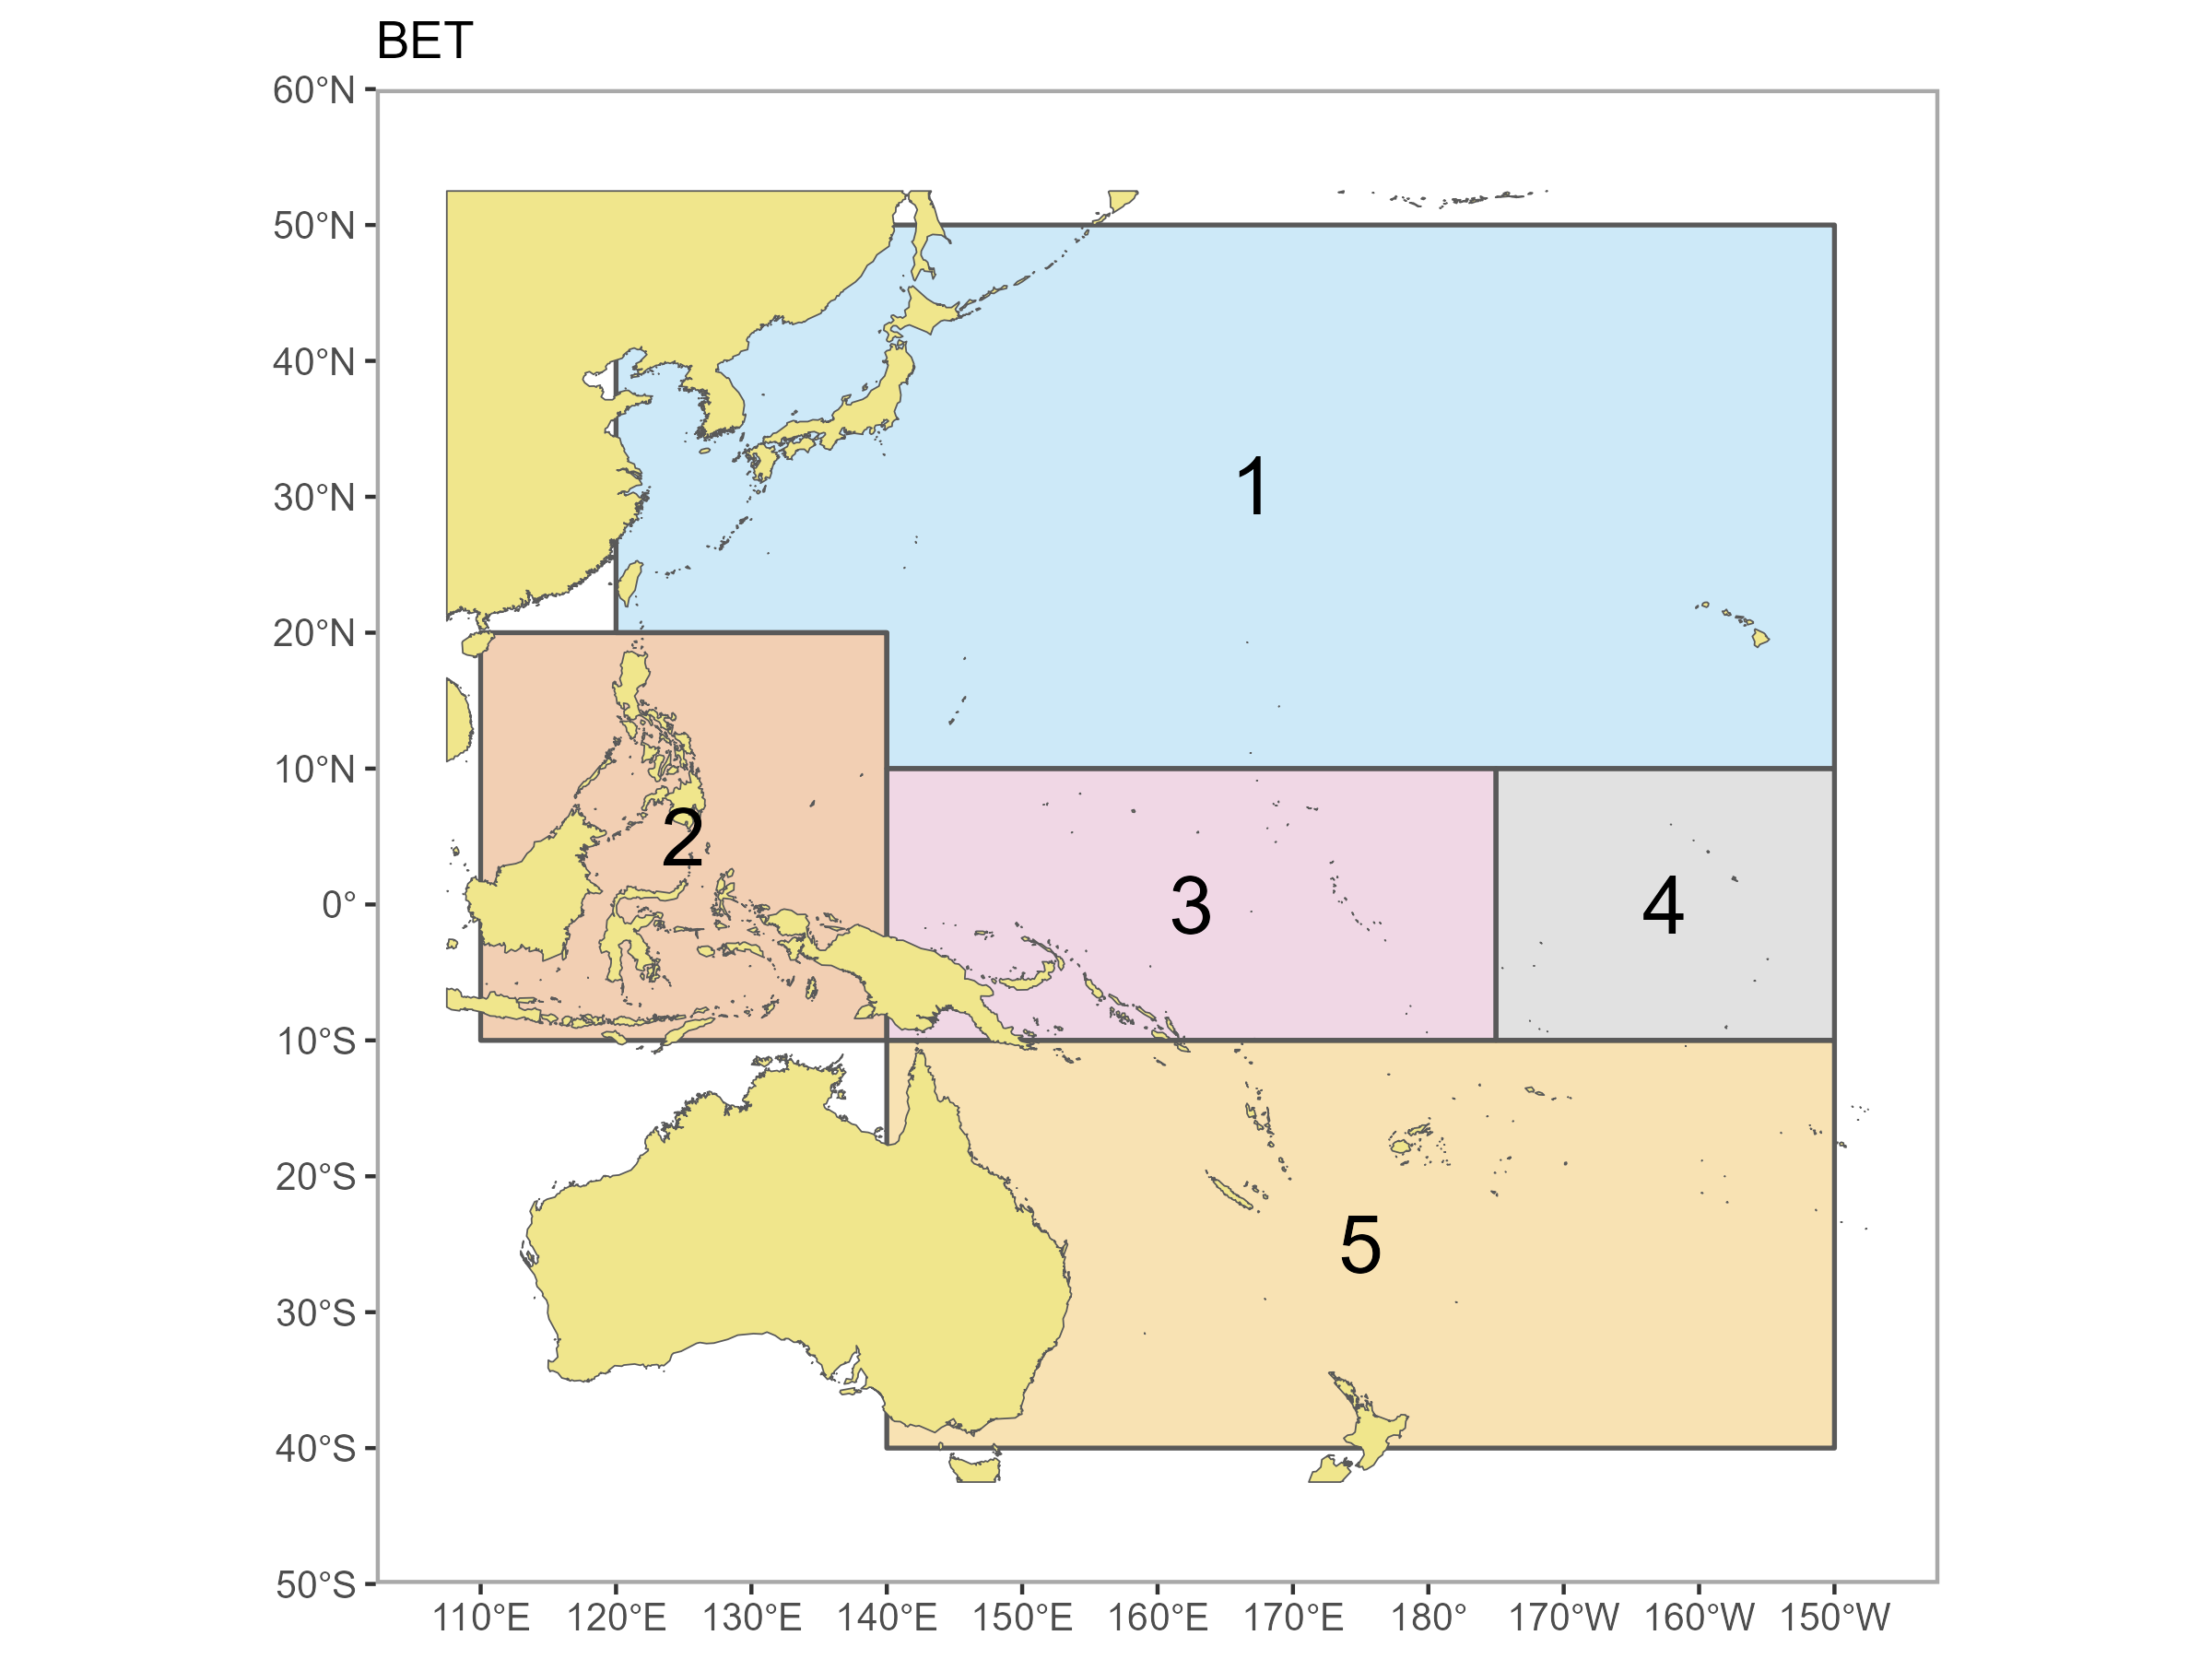
\includegraphics[width=1\linewidth,height=\textheight,keepaspectratio]{figures/map_5regions.png}
%DIFDELCMD <

%DIFDELCMD < }
%DIFDELCMD <

%DIFDELCMD < \caption{\label{fig-map-5regions}The geographical area covered by the
%DIFDELCMD < stock assessment and the boundaries of the five model regions used for
%DIFDELCMD < 2026 WCPO bigeye tuna assessment.}
%DIFDELCMD <

%DIFDELCMD < \end{figure}%%%
\DIFdelend \DIFaddbegin \begin{figure}[H]

\centering{

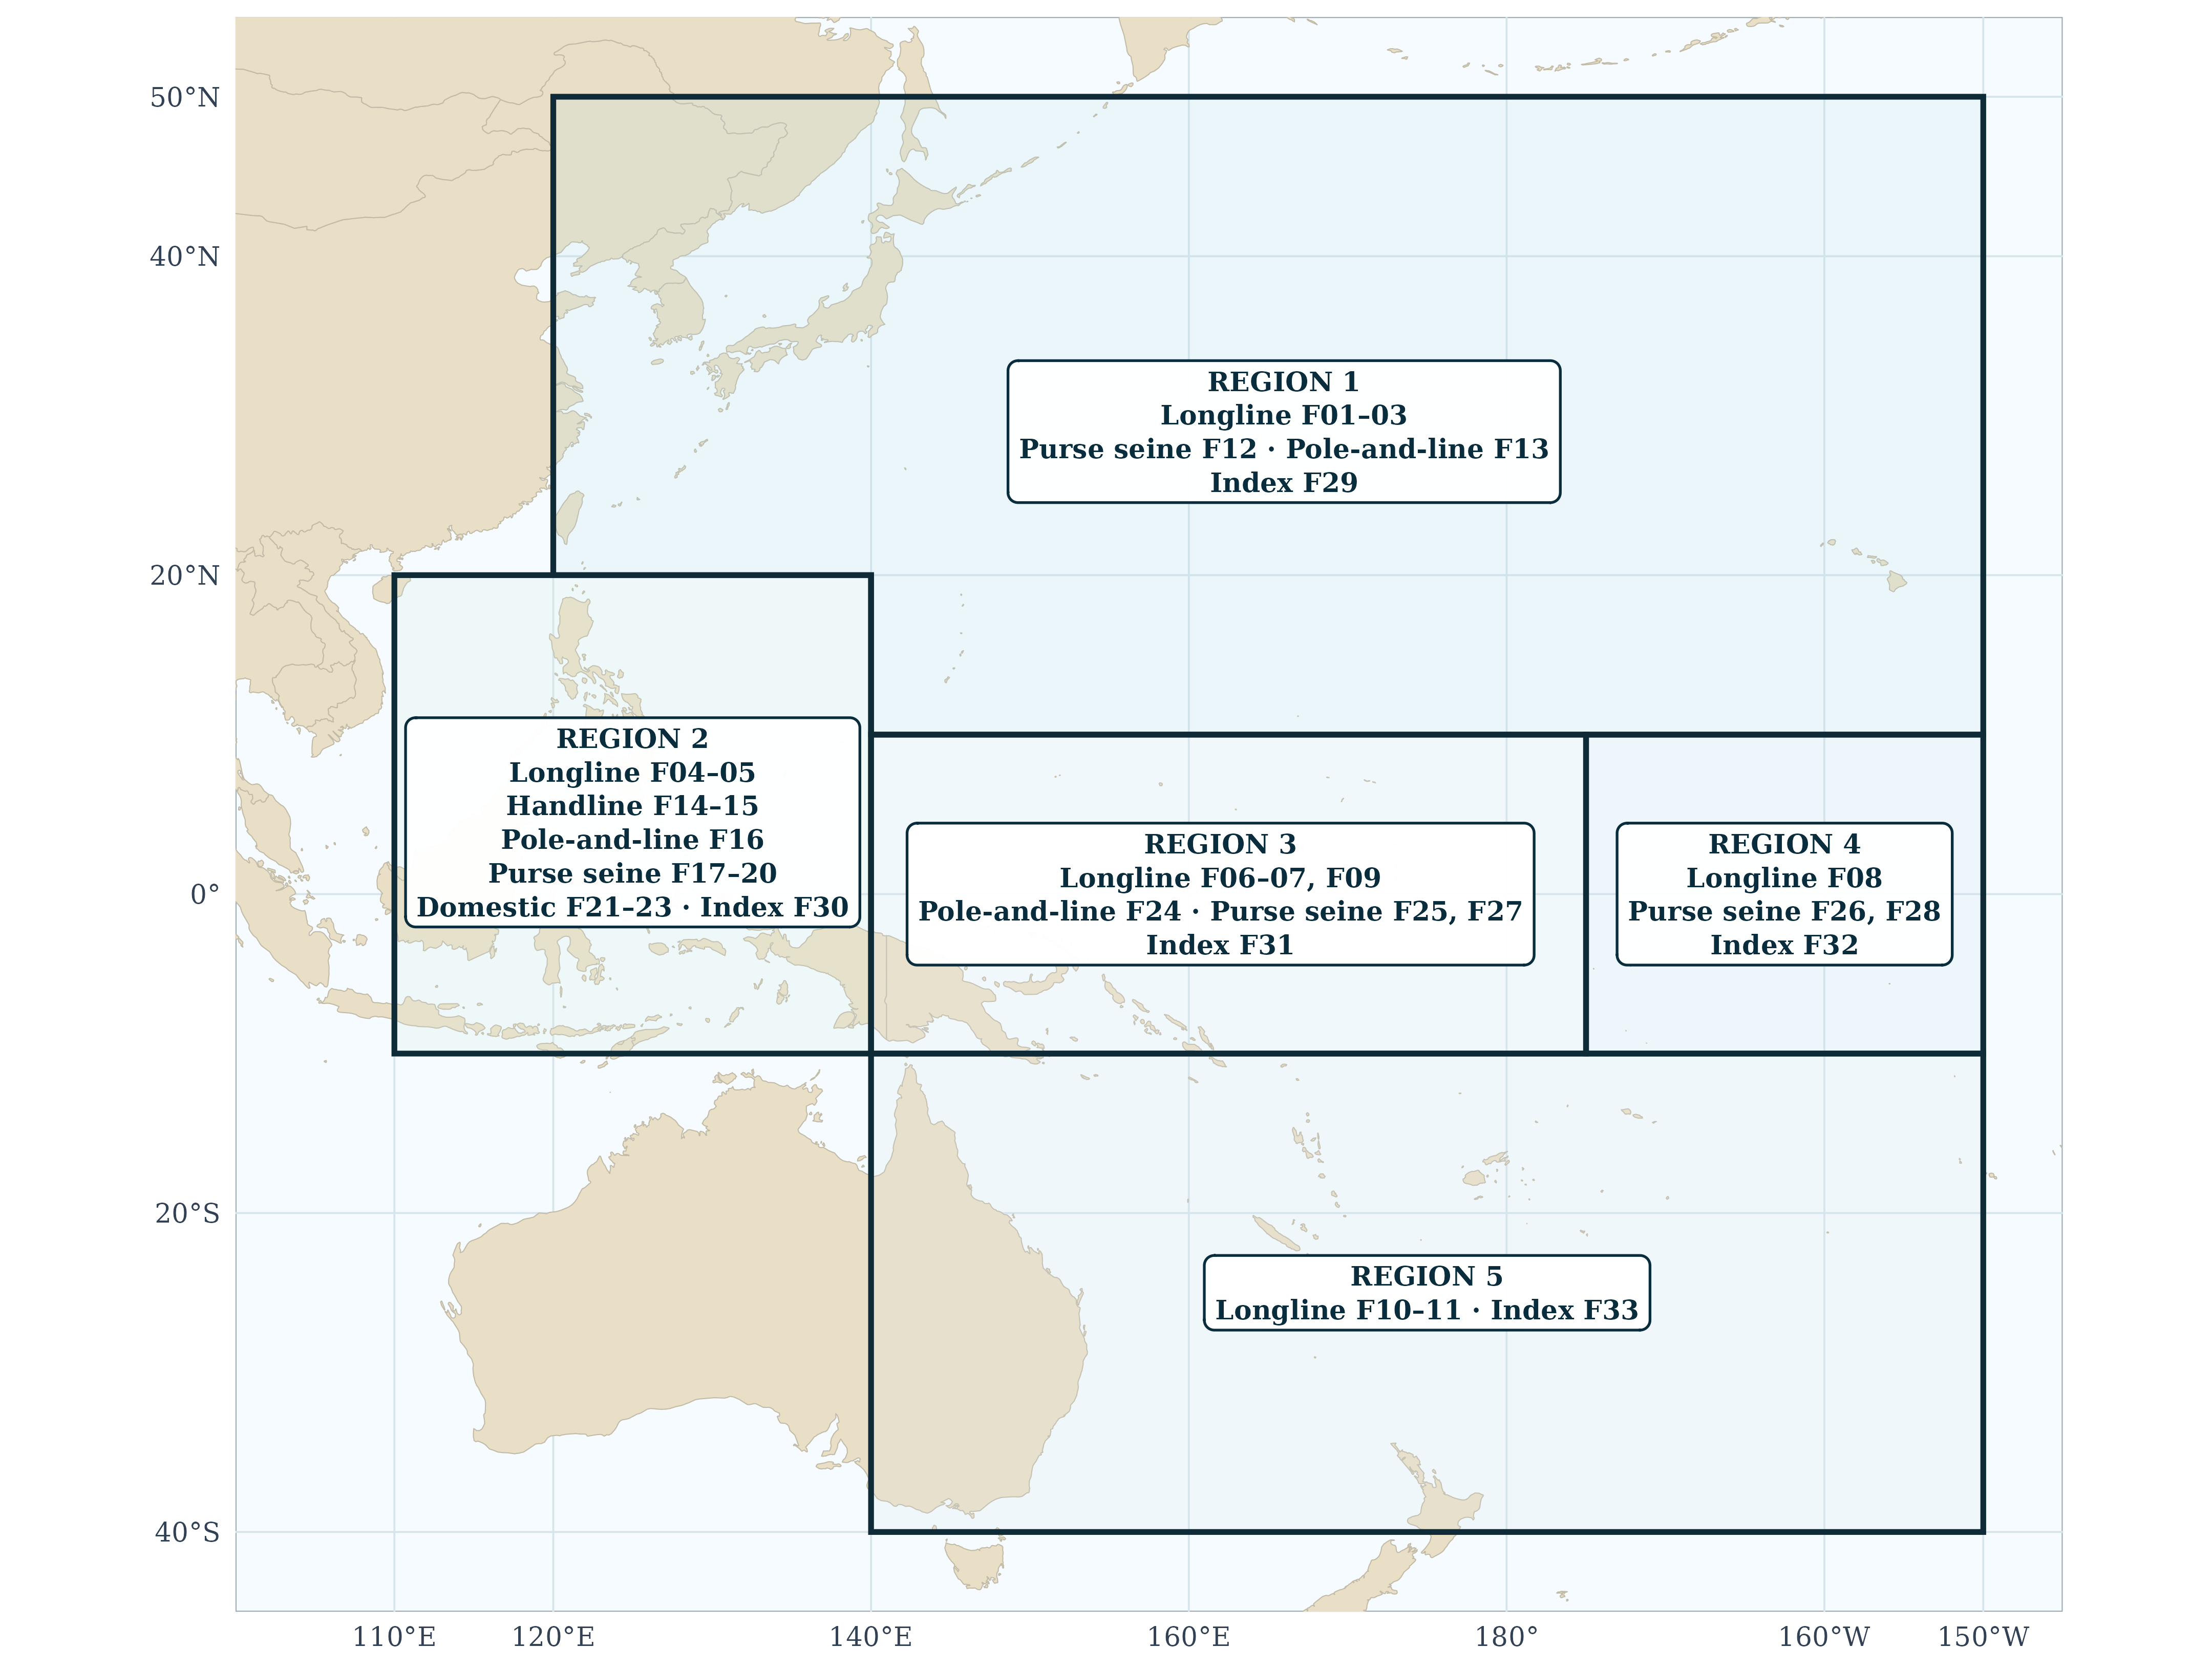
\includegraphics[width=1\linewidth,height=\textheight,keepaspectratio]{figures_new/region-map.png}

}

\caption{\label{fig-map-5regions}Five-region spatial structure used by
the 2026 diagnostic model. Labels identify the fitted fisheries in each
region by gear and fishery ID; the IDs correspond to
Table~\ref{tbl-fisheries-definitions}.}

\end{figure}\DIFaddend %

\begin{figure}[H]

\centering{

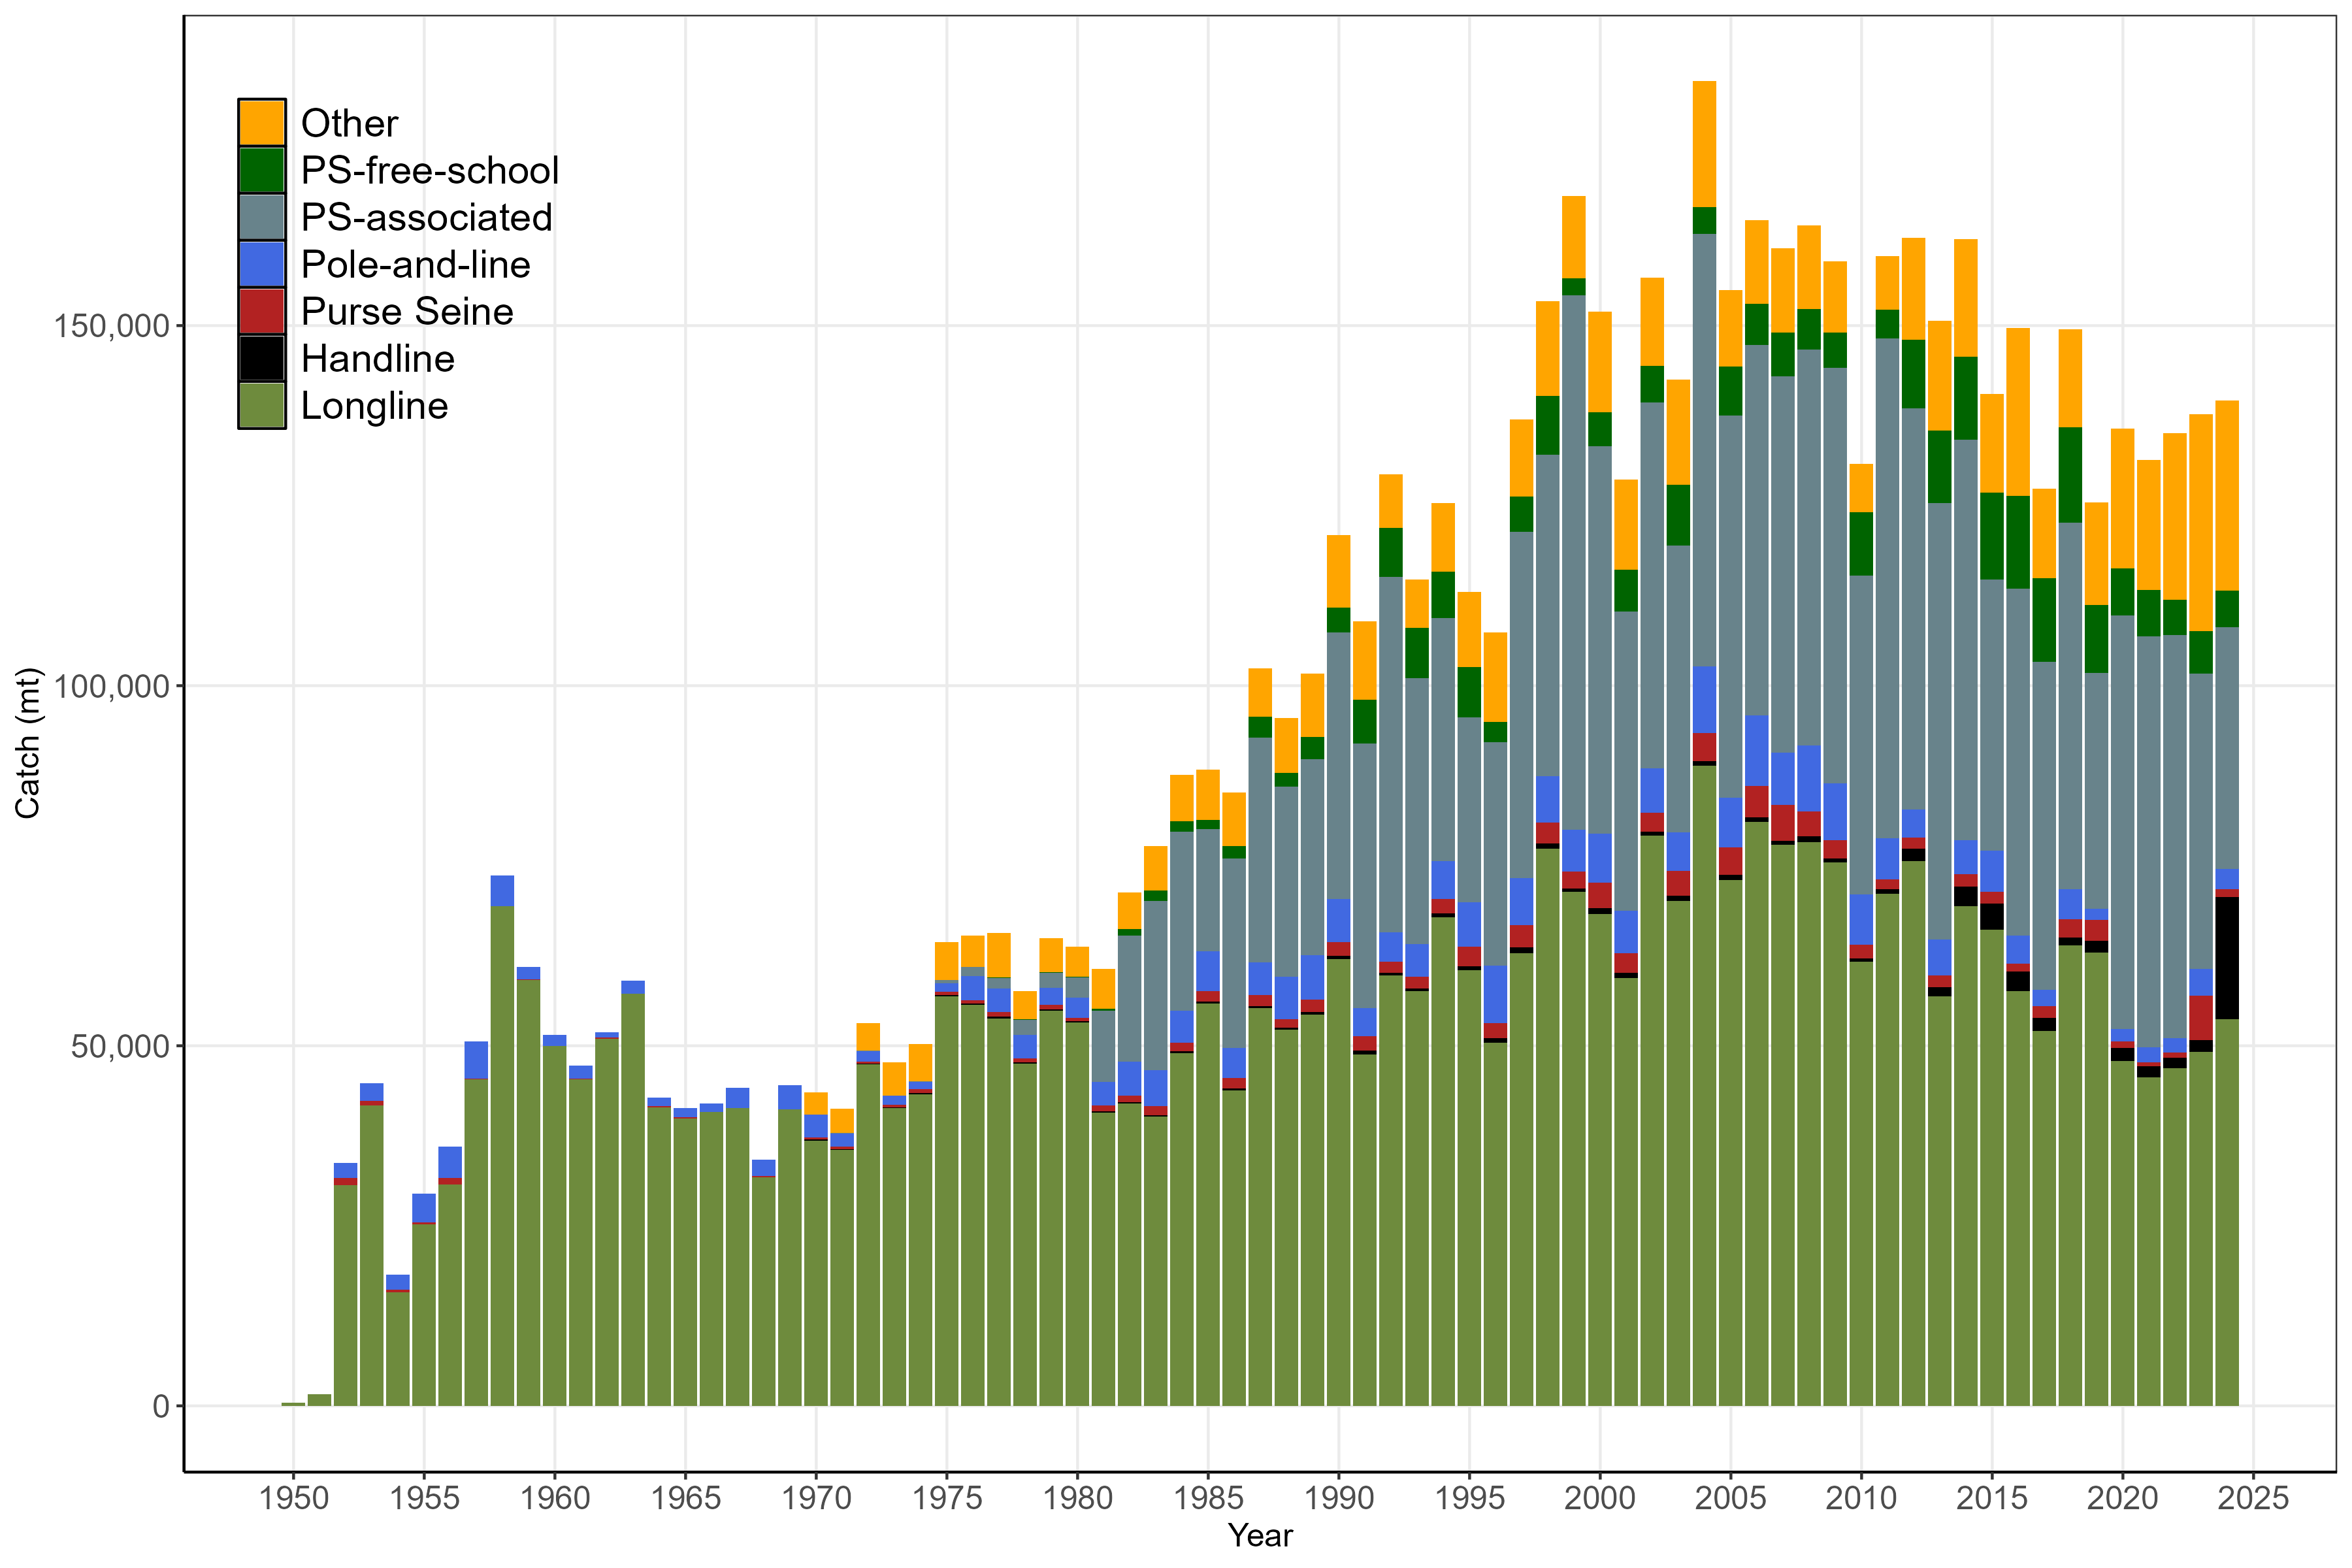
\includegraphics[width=1\linewidth,height=\textheight,keepaspectratio]{figures/catch_hist_full.png}

}

\caption{\label{fig-catch-hist-full}Annual catches of bigeye by gear
type in the WCPO area covered by the assessment.}

\end{figure}%

\DIFdelbegin %DIFDELCMD < \begin{figure}[H]
%DIFDELCMD <

%DIFDELCMD < \centering{
%DIFDELCMD <

%DIFDELCMD < 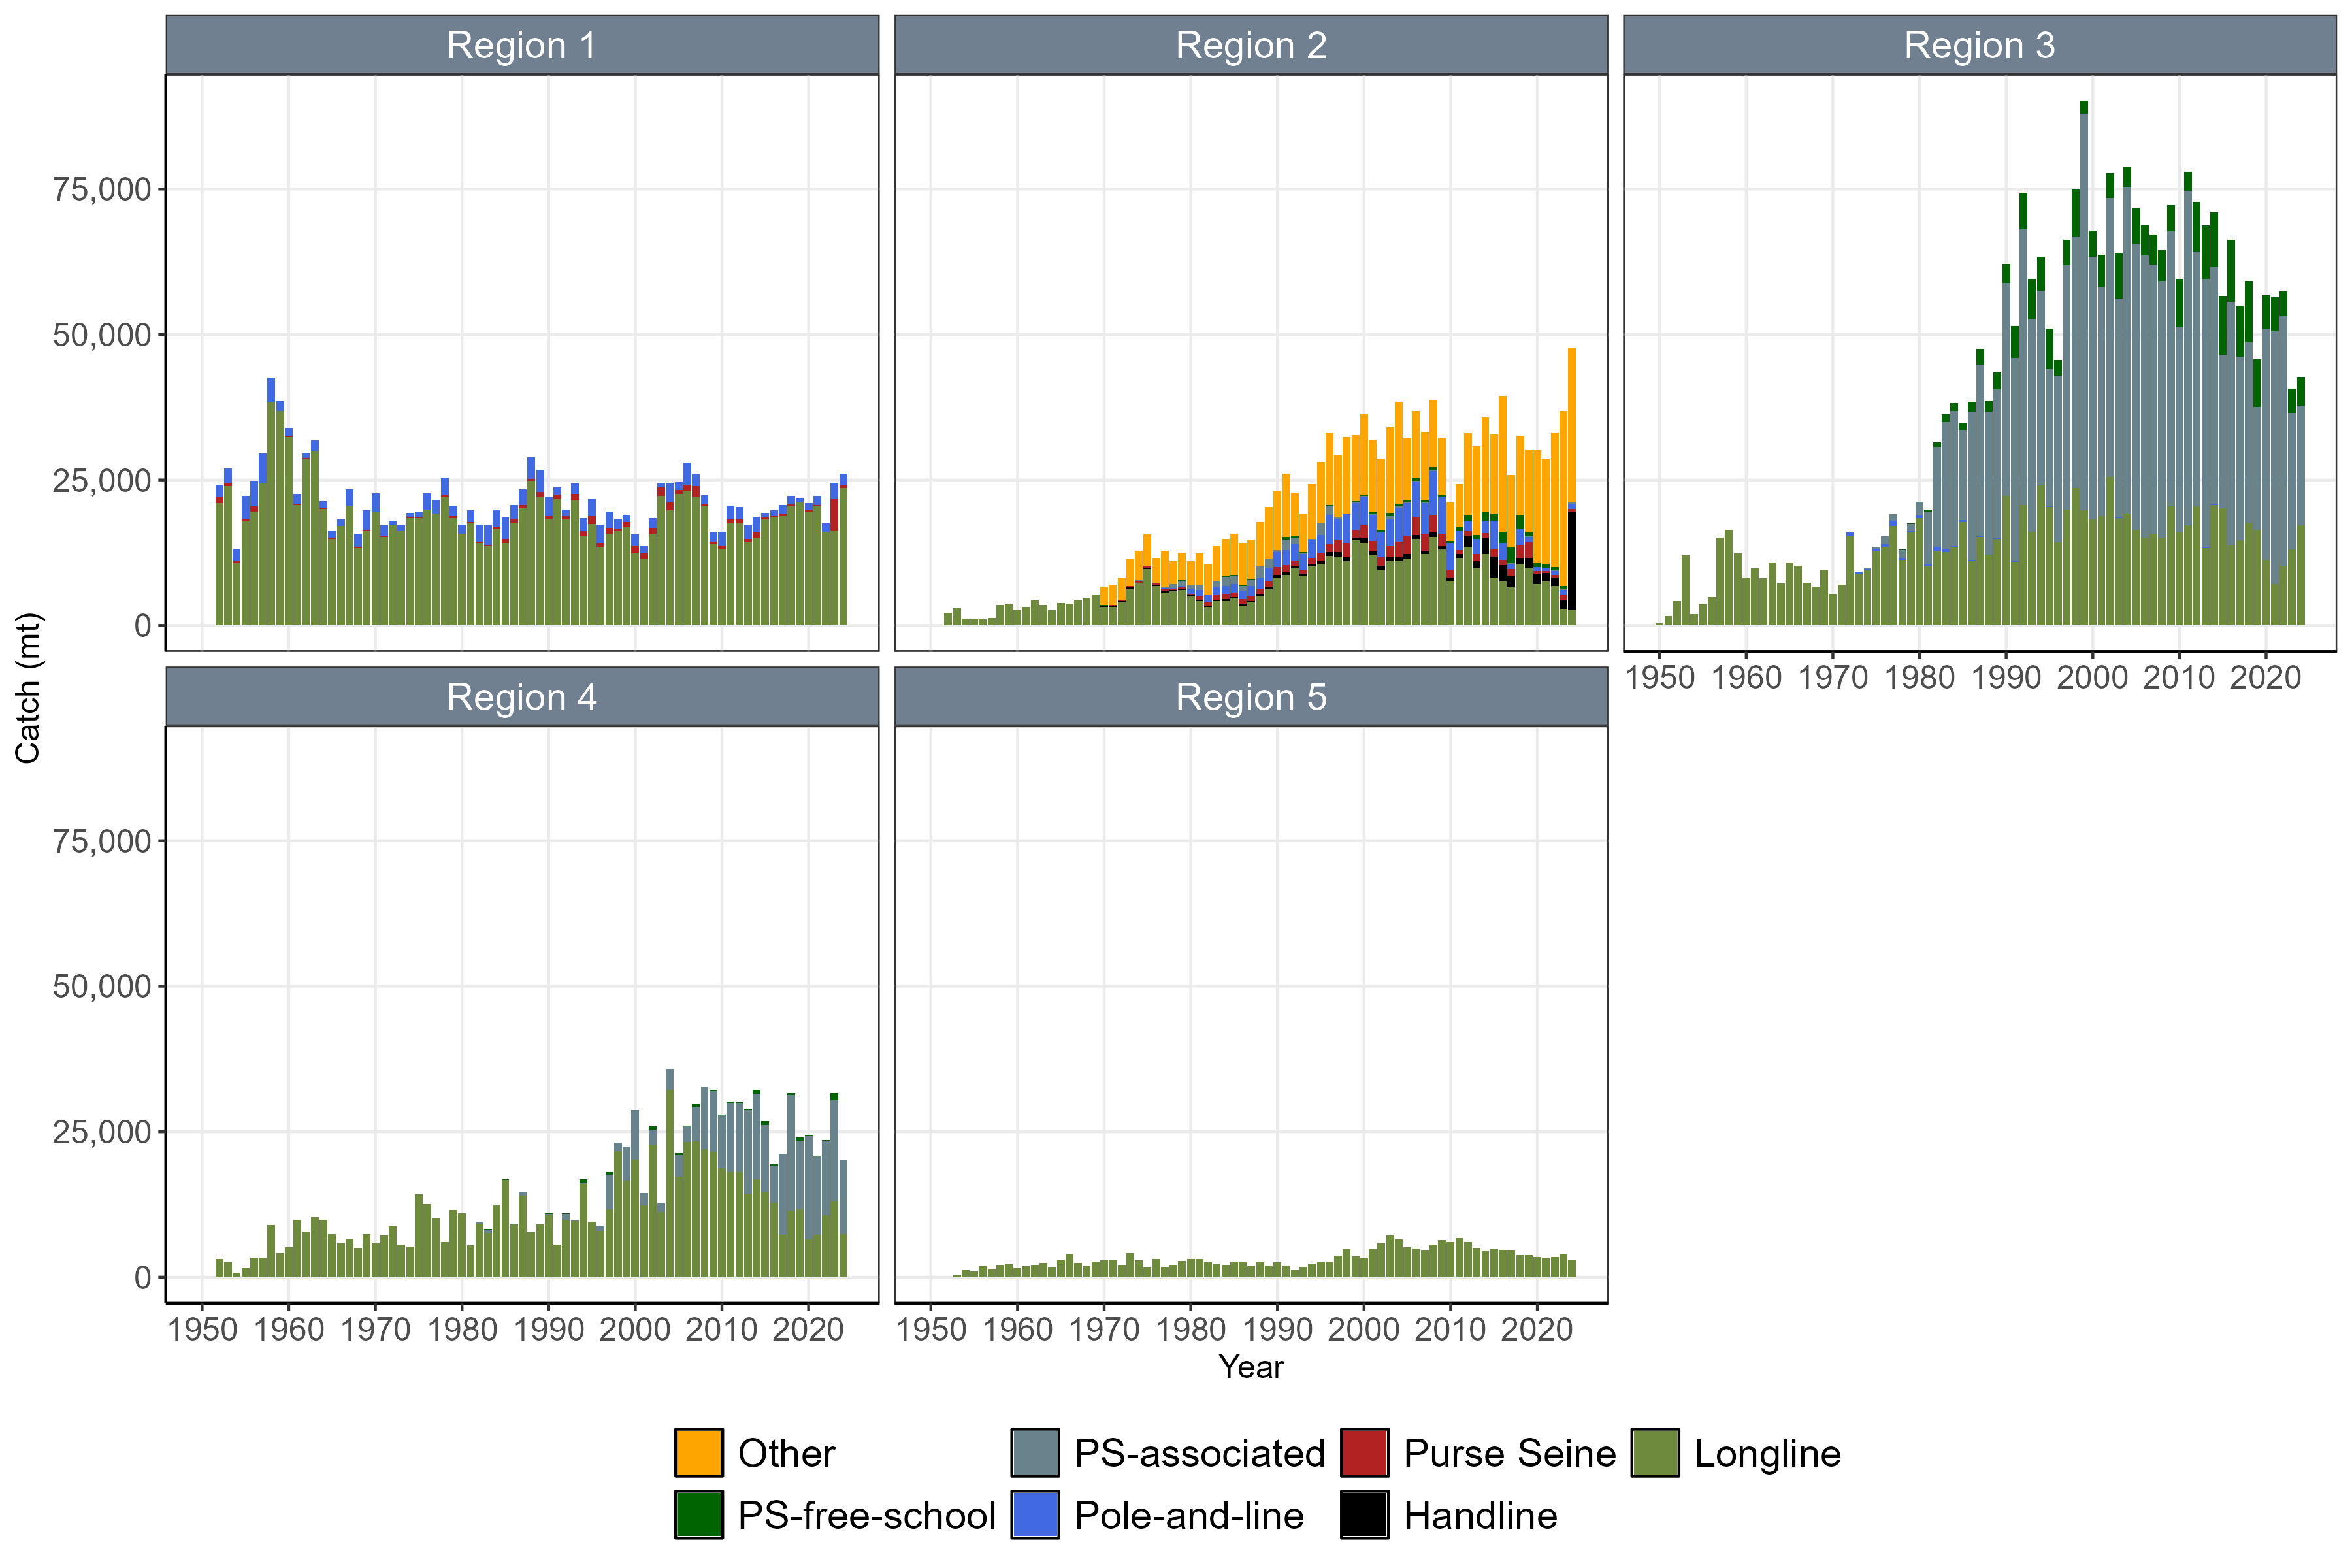
\includegraphics[width=1\linewidth,height=\textheight,keepaspectratio]{figures/catch_hist_regional.png}
%DIFDELCMD <

%DIFDELCMD < }
%DIFDELCMD <

%DIFDELCMD < \caption{\label{fig-catch-hist-regional}Annual catches of bigeye by gear
%DIFDELCMD < type for each of the nine model regions.}
%DIFDELCMD <

%DIFDELCMD < \end{figure}%%%
\DIFdelend \DIFaddbegin \begin{figure}[H]

\centering{

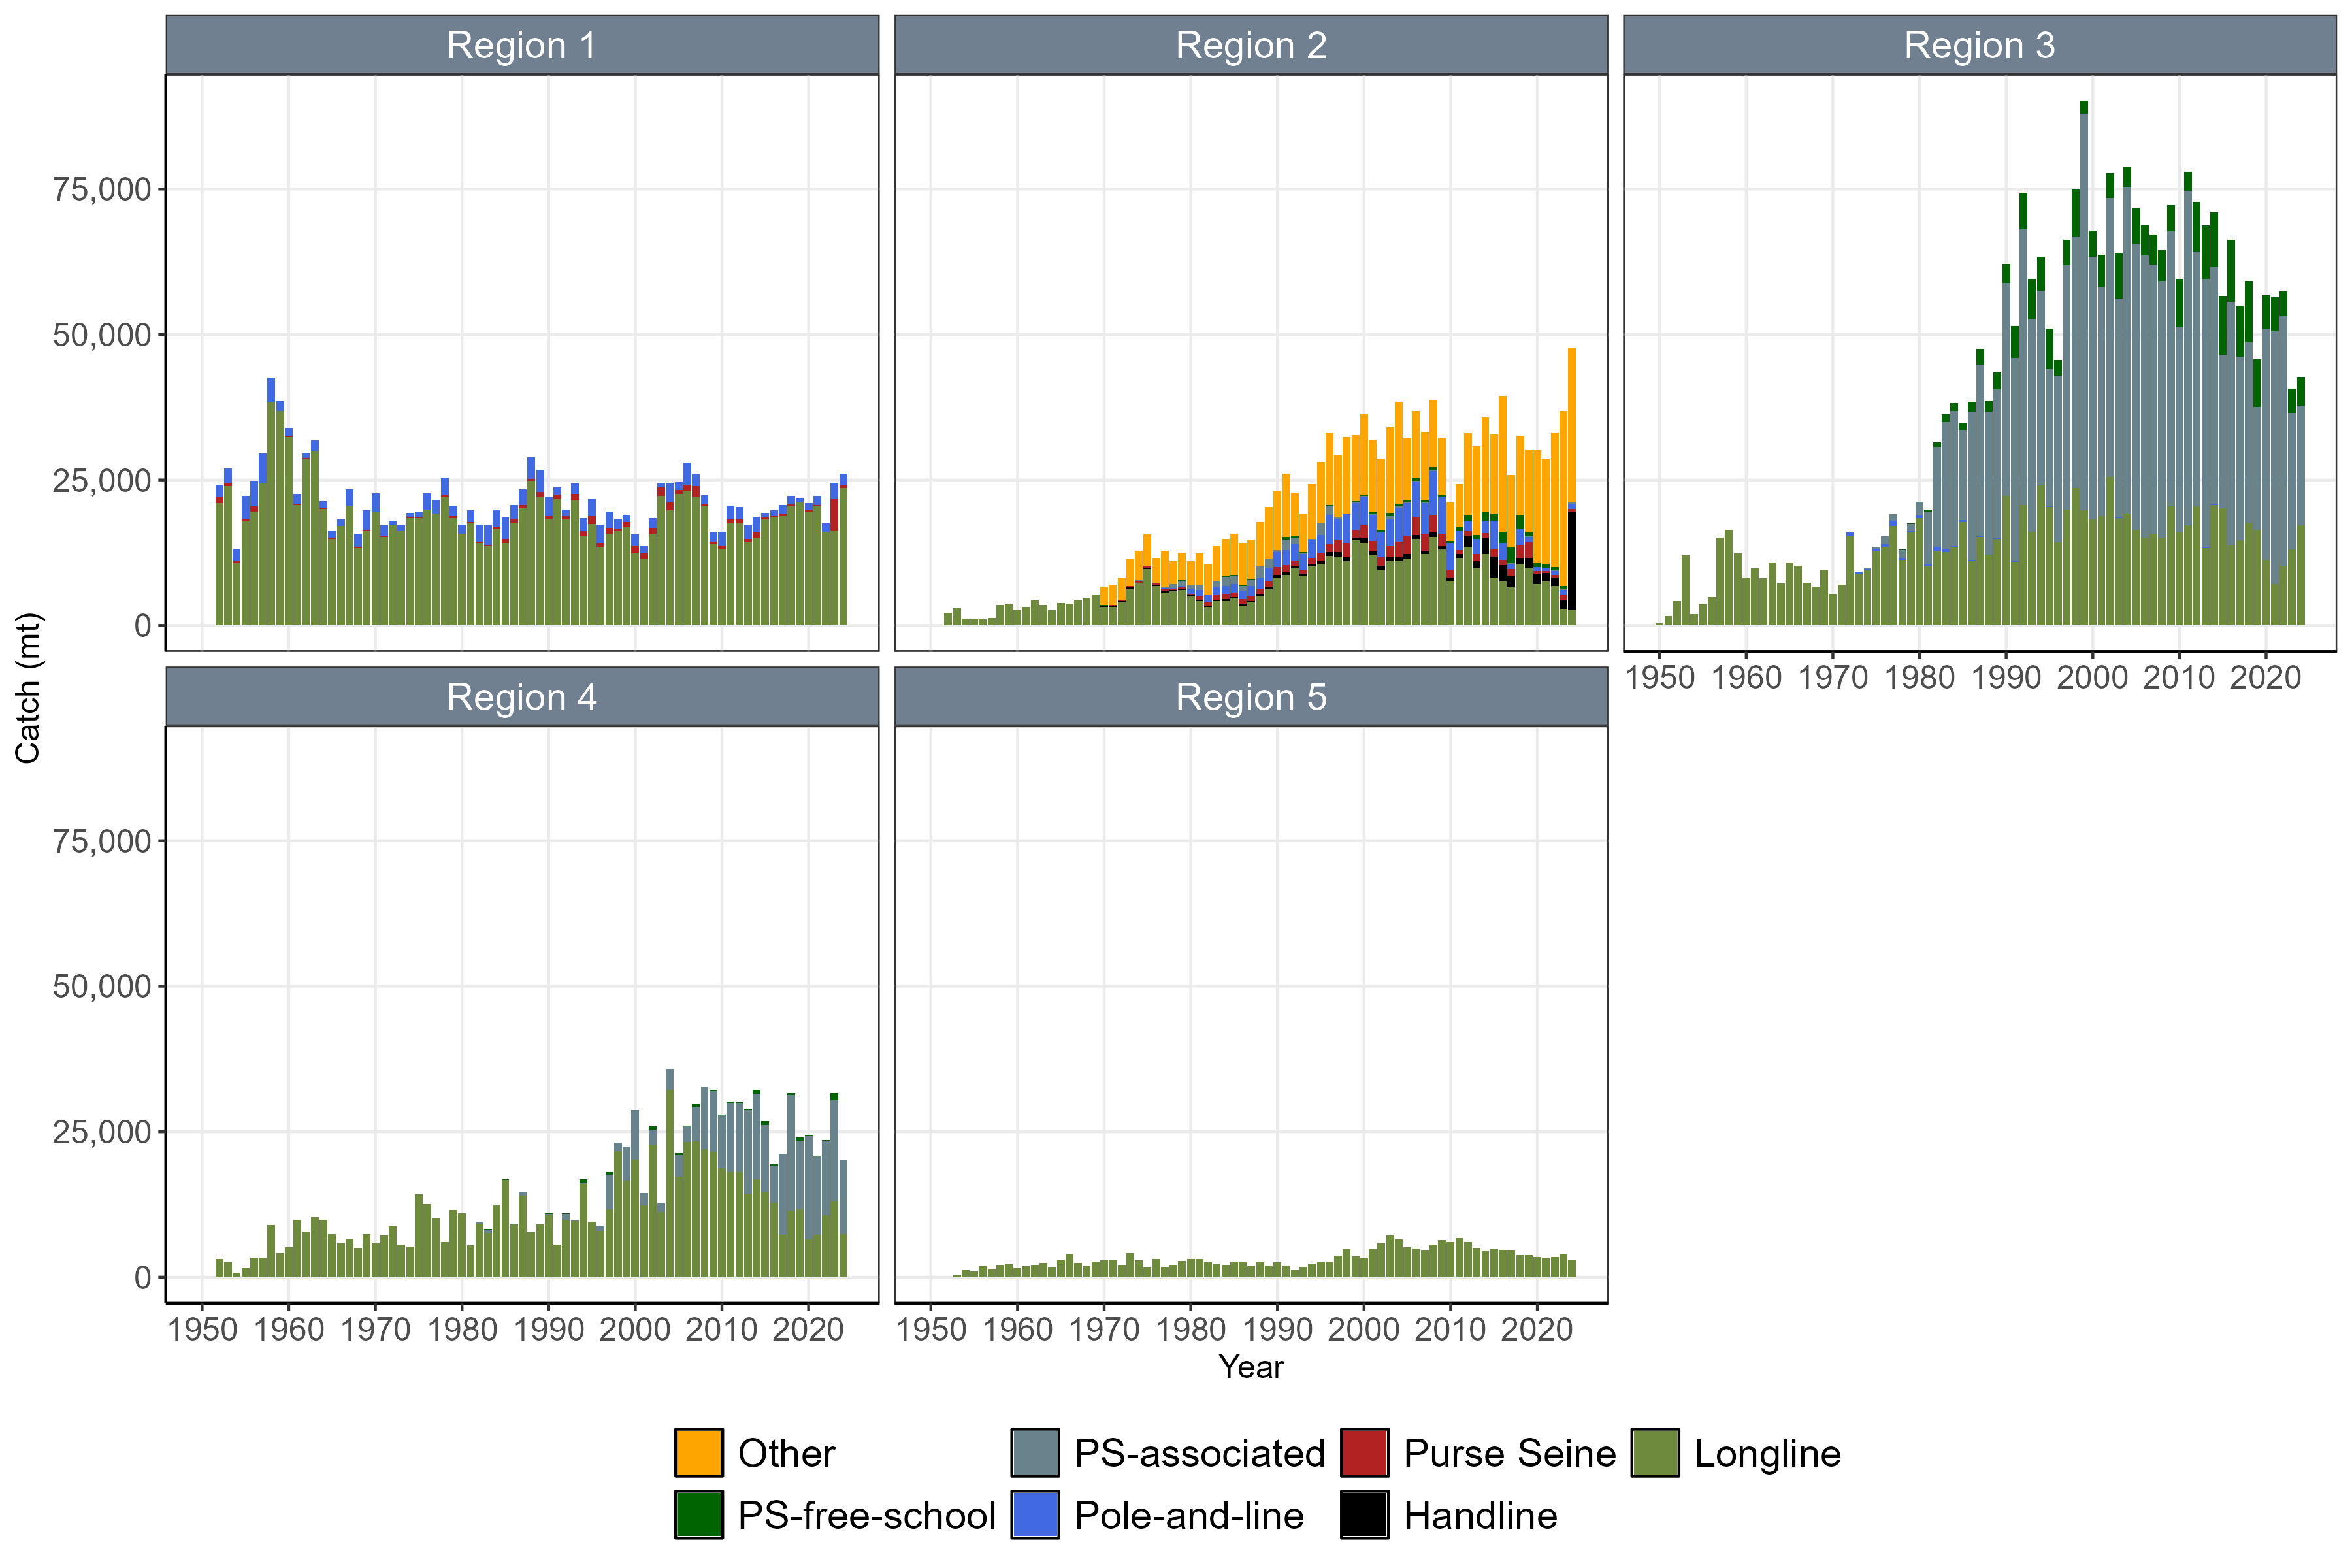
\includegraphics[width=1\linewidth,height=\textheight,keepaspectratio]{figures/catch_hist_regional.png}

}

\caption{\label{fig-catch-hist-regional}Annual catches of bigeye tuna by
gear type for each of the five model regions.}

\end{figure}\DIFaddend %

\begin{figure}[H]

\centering{

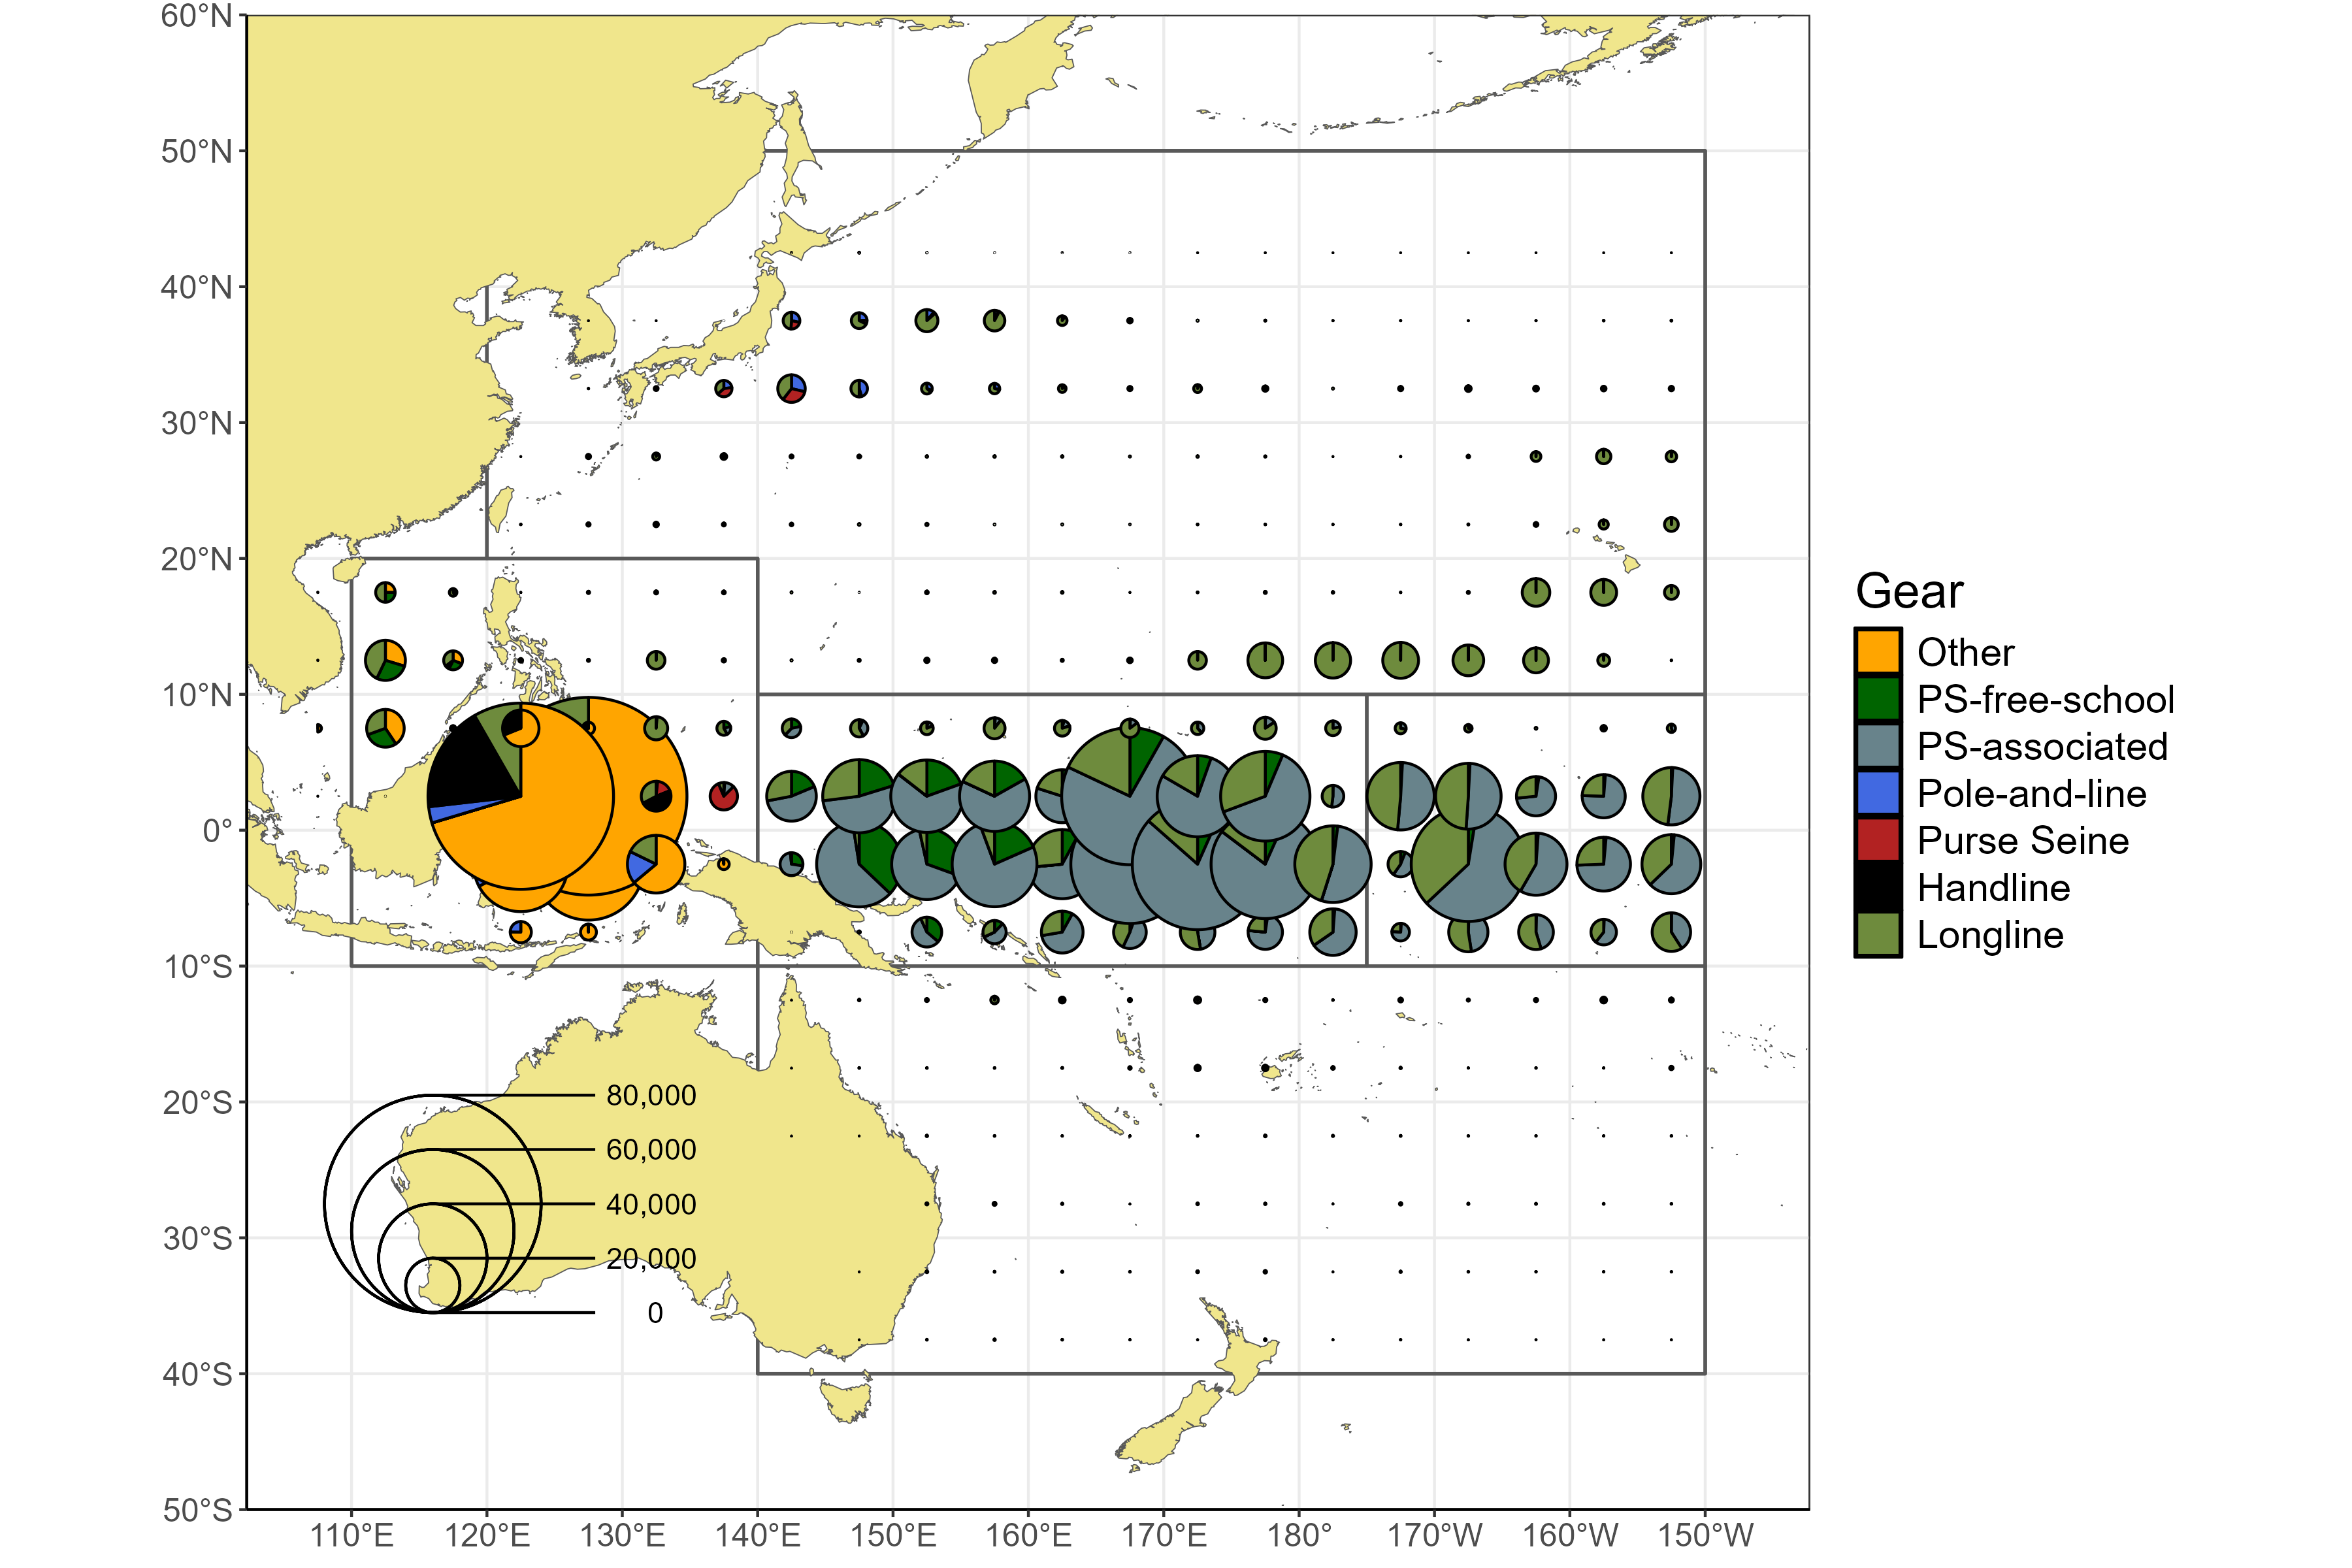
\includegraphics[width=1\linewidth,height=\textheight,keepaspectratio]{figures/catch_map.png}

}

\caption{\label{fig-catch-map}Distribution and magnitude of bigeye
catches (mt) by gear type summed over the last 10 years (2015-2024) for
5 x 5 degree cells.}

\end{figure}%

\DIFdelbegin %DIFDELCMD < \begin{figure}[H]
%DIFDELCMD <

%DIFDELCMD < \centering{
%DIFDELCMD <

%DIFDELCMD < 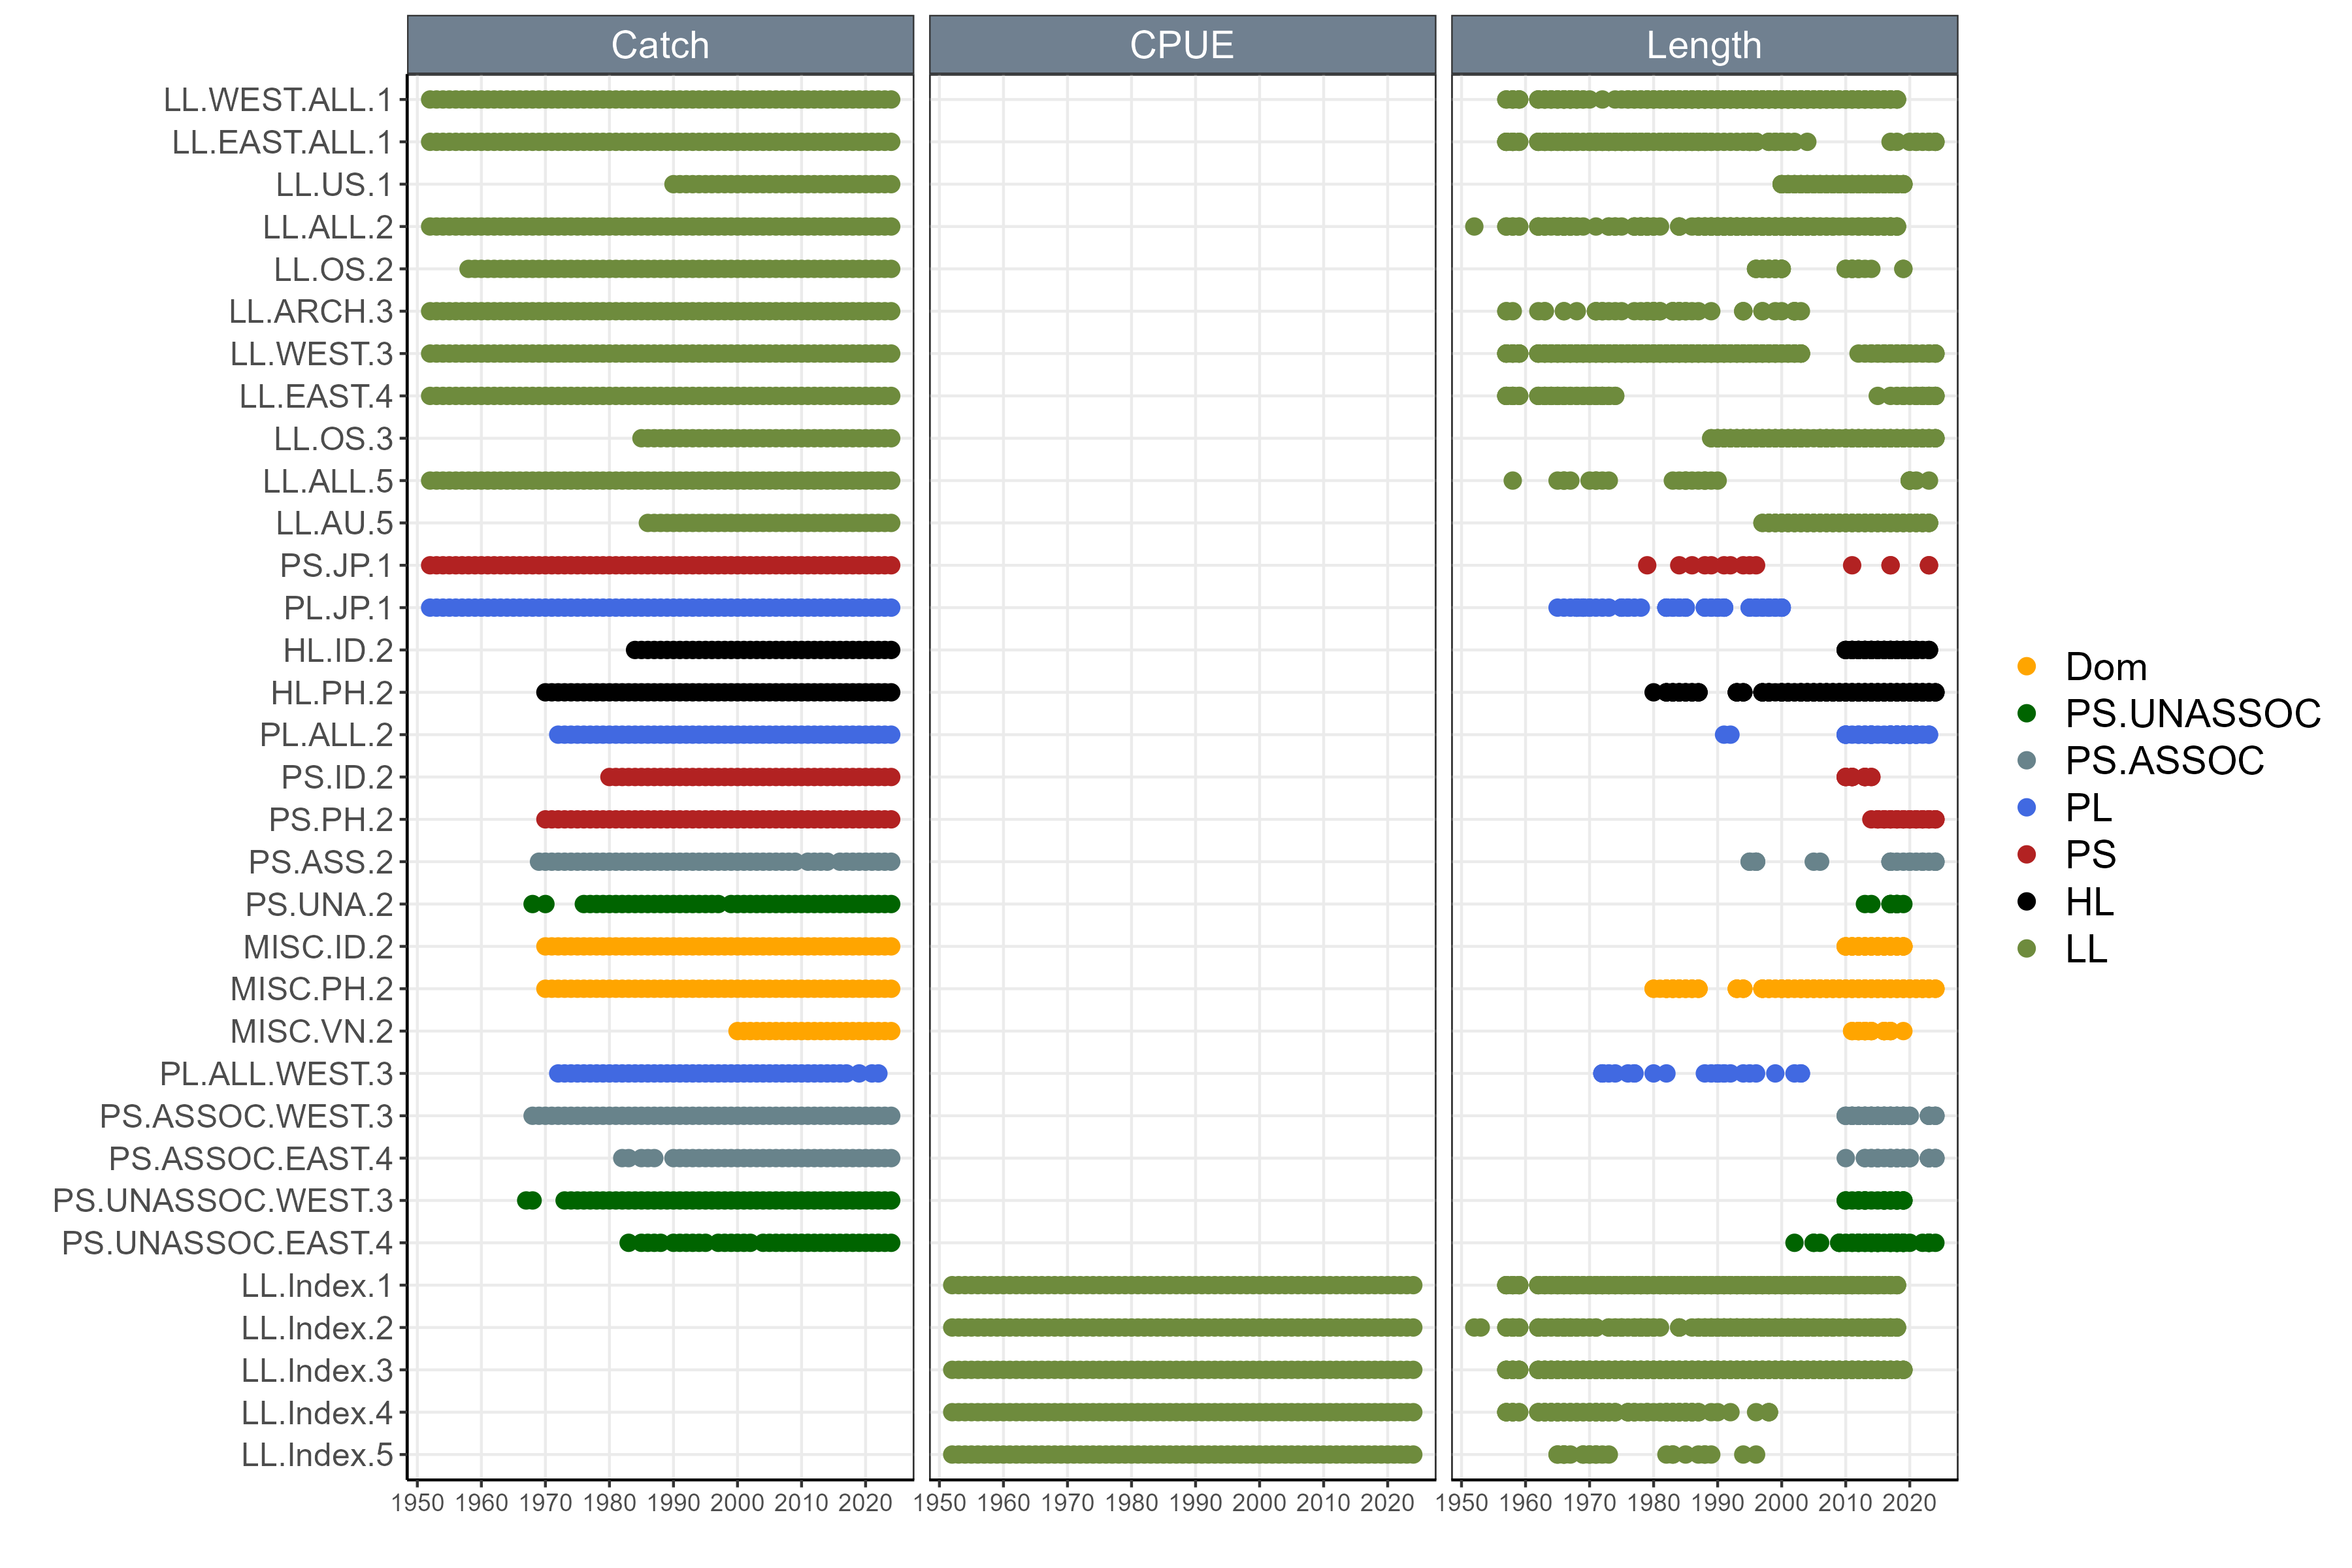
\includegraphics[width=1\linewidth,height=\textheight,keepaspectratio]{figures/data_coverage_tile.png}
%DIFDELCMD <

%DIFDELCMD < }
%DIFDELCMD <

%DIFDELCMD < \caption{\label{fig-data-coverage-tile}Summary of data coverage by
%DIFDELCMD < fishery for the WCPO 2023 bigeye assessment. I=index fisheries,
%DIFDELCMD < L=longline, P=pole and line, S=purse seine (unspecified), SA=purse seine
%DIFDELCMD < associated, SU=purse seine unassociated, Z=miscellaneous gears.}
%DIFDELCMD <

%DIFDELCMD < \end{figure}%%%
\DIFdelend \DIFaddbegin \begin{figure}[H]

\centering{

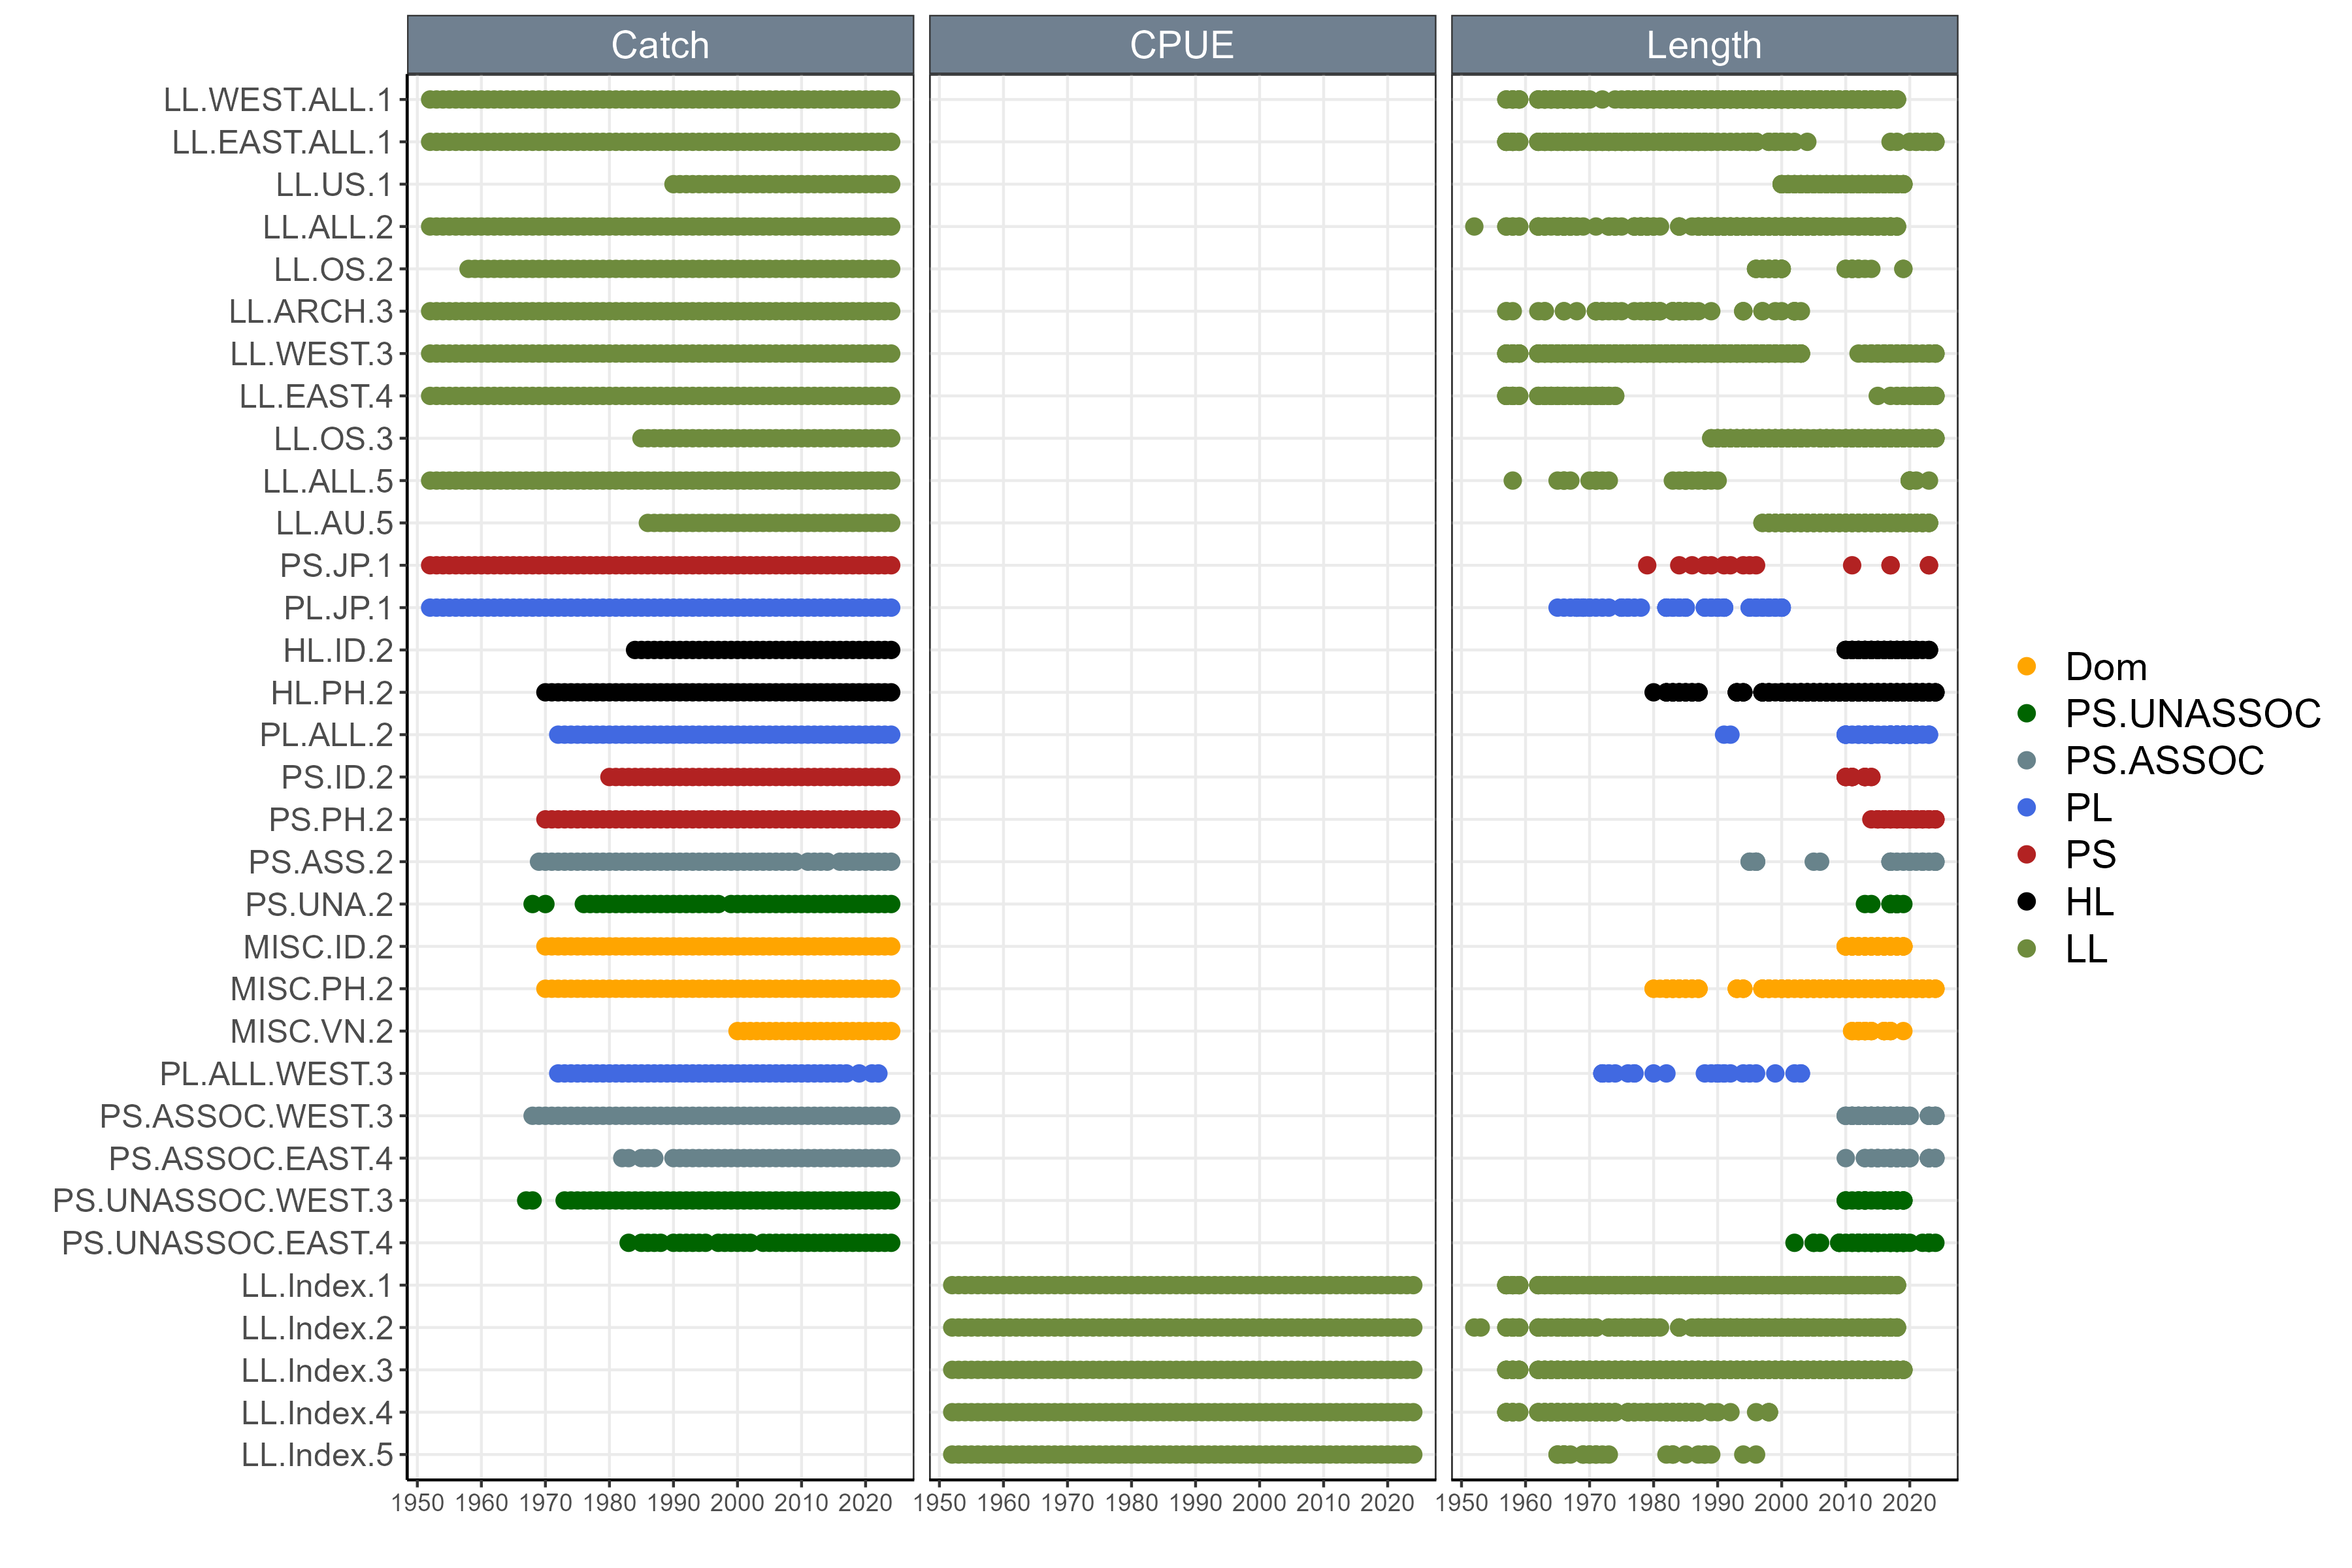
\includegraphics[width=1\linewidth,height=\textheight,keepaspectratio]{figures/data_coverage_tile.png}

}

\caption{\label{fig-data-coverage-tile}Summary of data coverage by
fishery for the 2026 WCPO bigeye tuna assessment. I denotes index
fisheries, L longline, P pole-and-line, S purse seine (unspecified), SA
associated purse seine, SU unassociated purse seine and Z miscellaneous
gears.}

\end{figure}\DIFaddend %

\begin{figure}[H]

\centering{

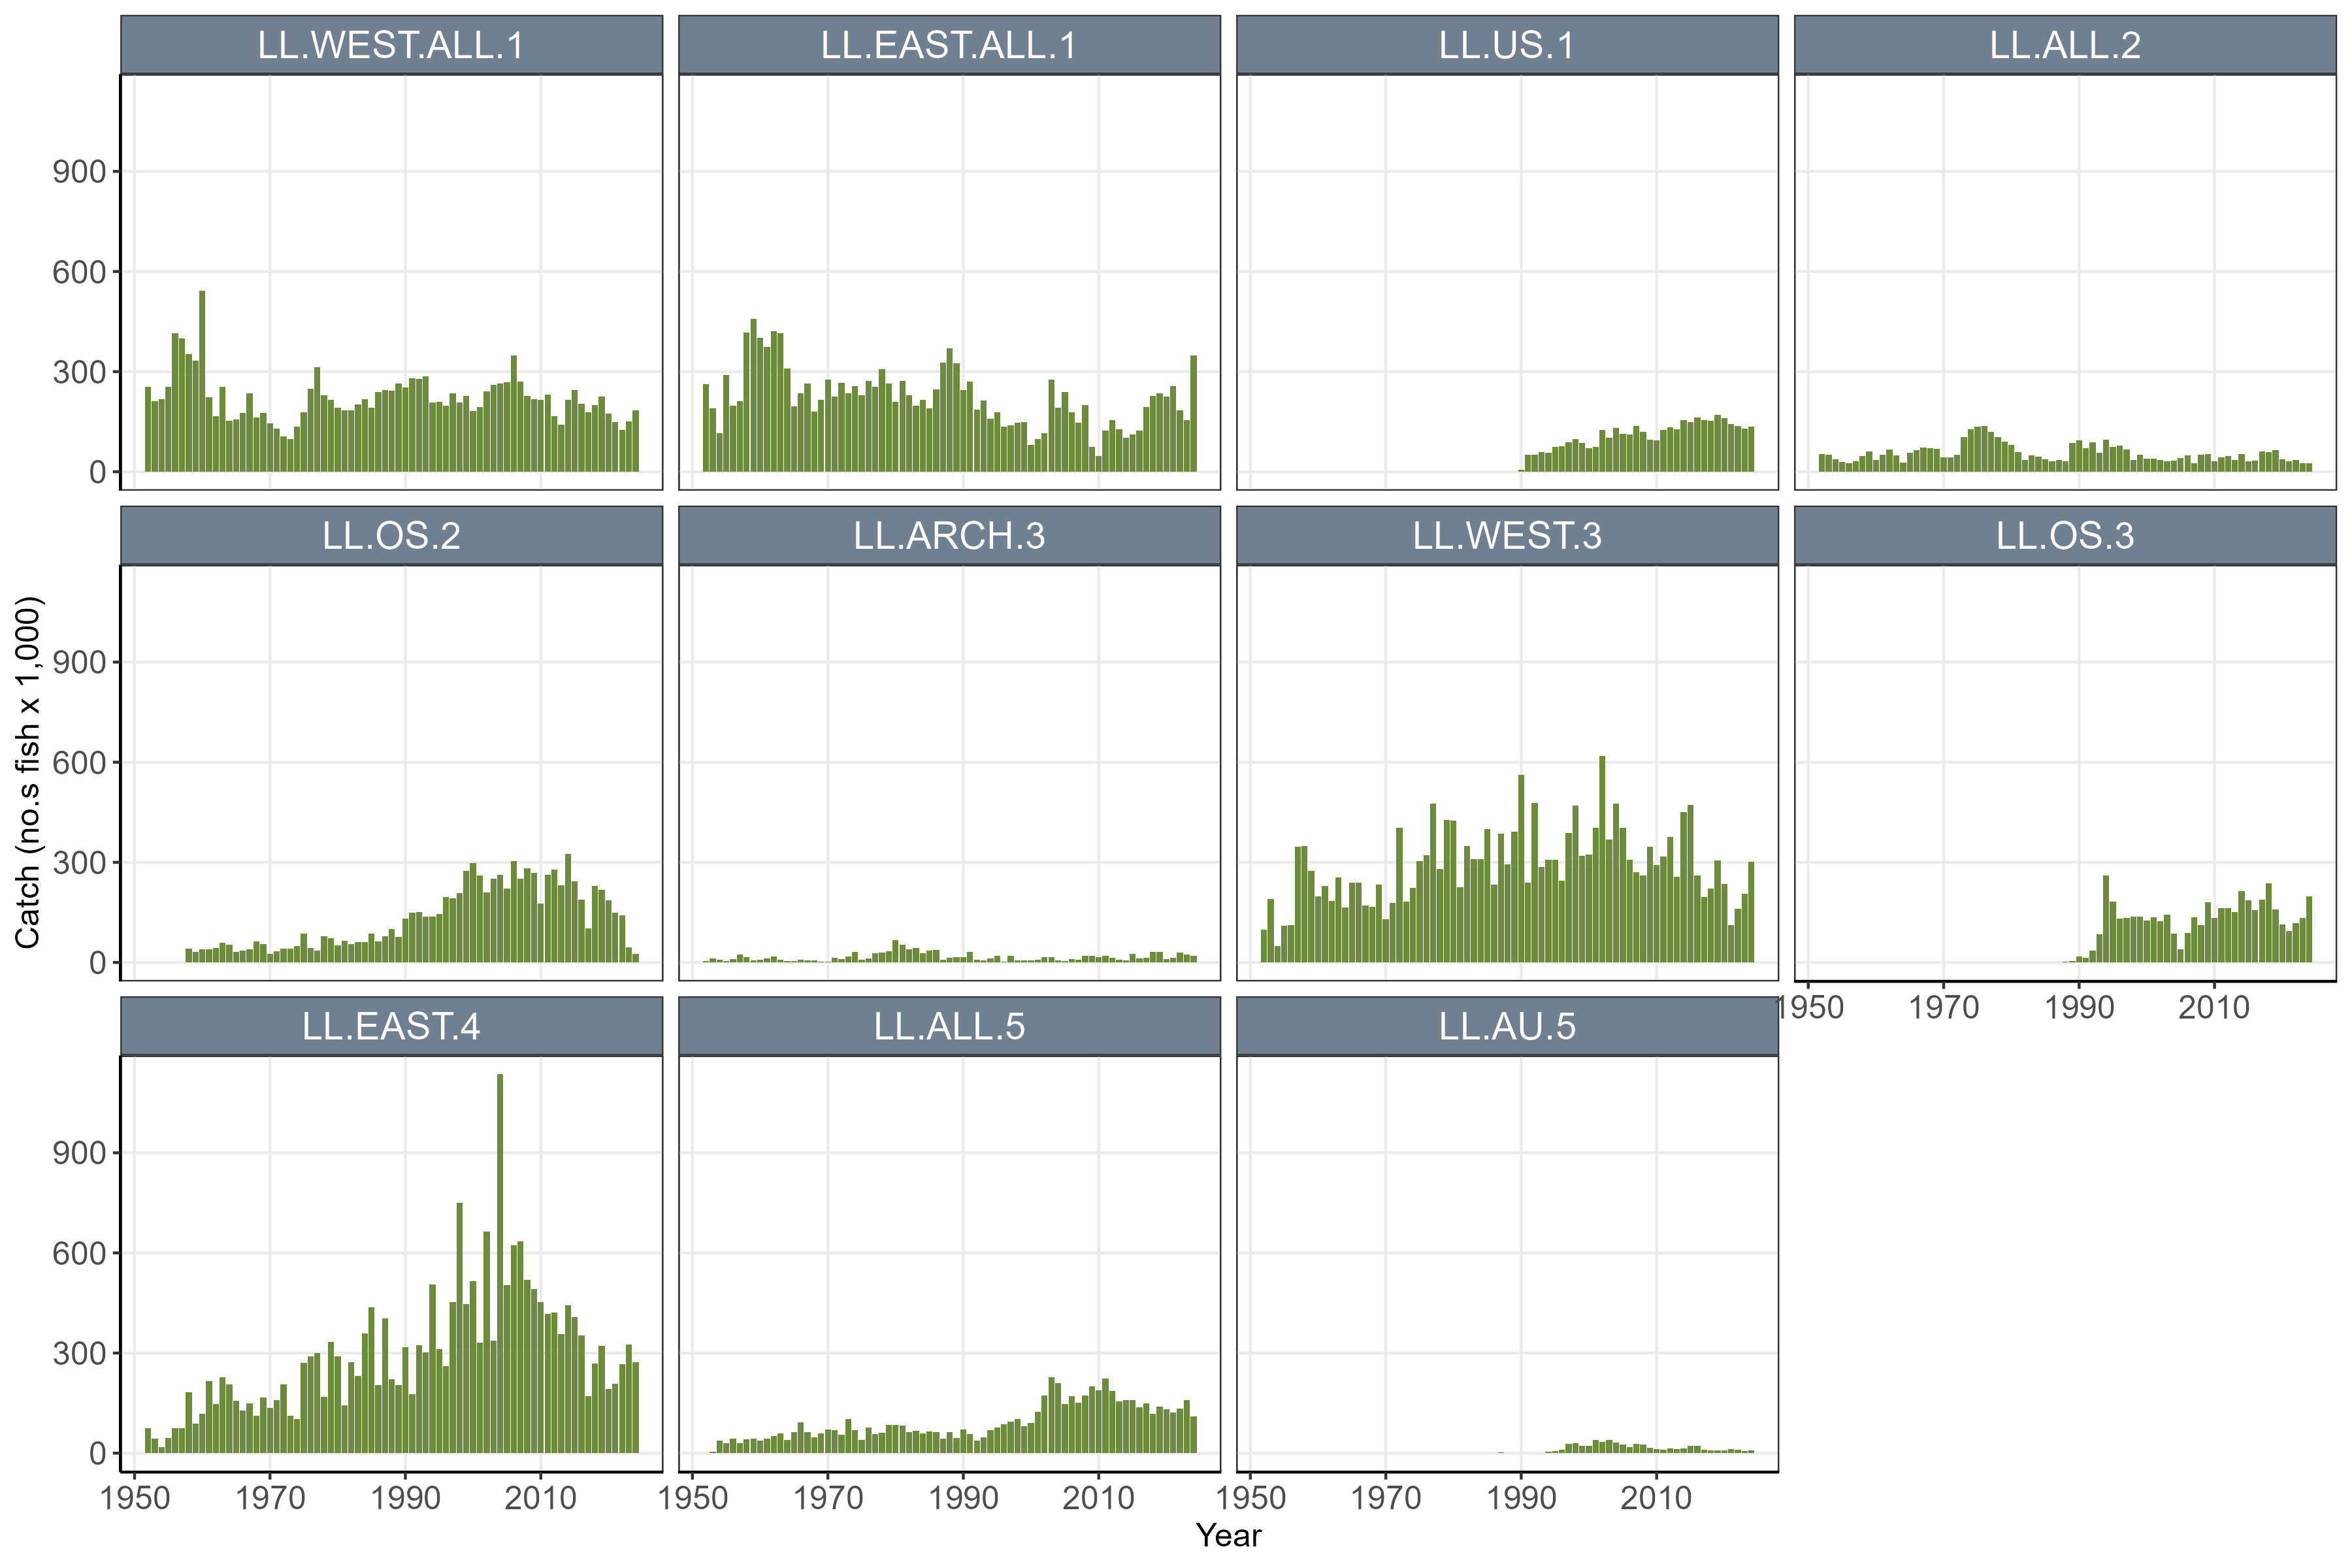
\includegraphics[width=1\linewidth,height=\textheight,keepaspectratio]{figures/catch_by_fishery_longline.png}

}

\caption{\label{fig-catch-by-fishery-longline}Time series of catches
(numbers of fish) by fishery: longline.}

\end{figure}%

\begin{figure}[H]

\centering{

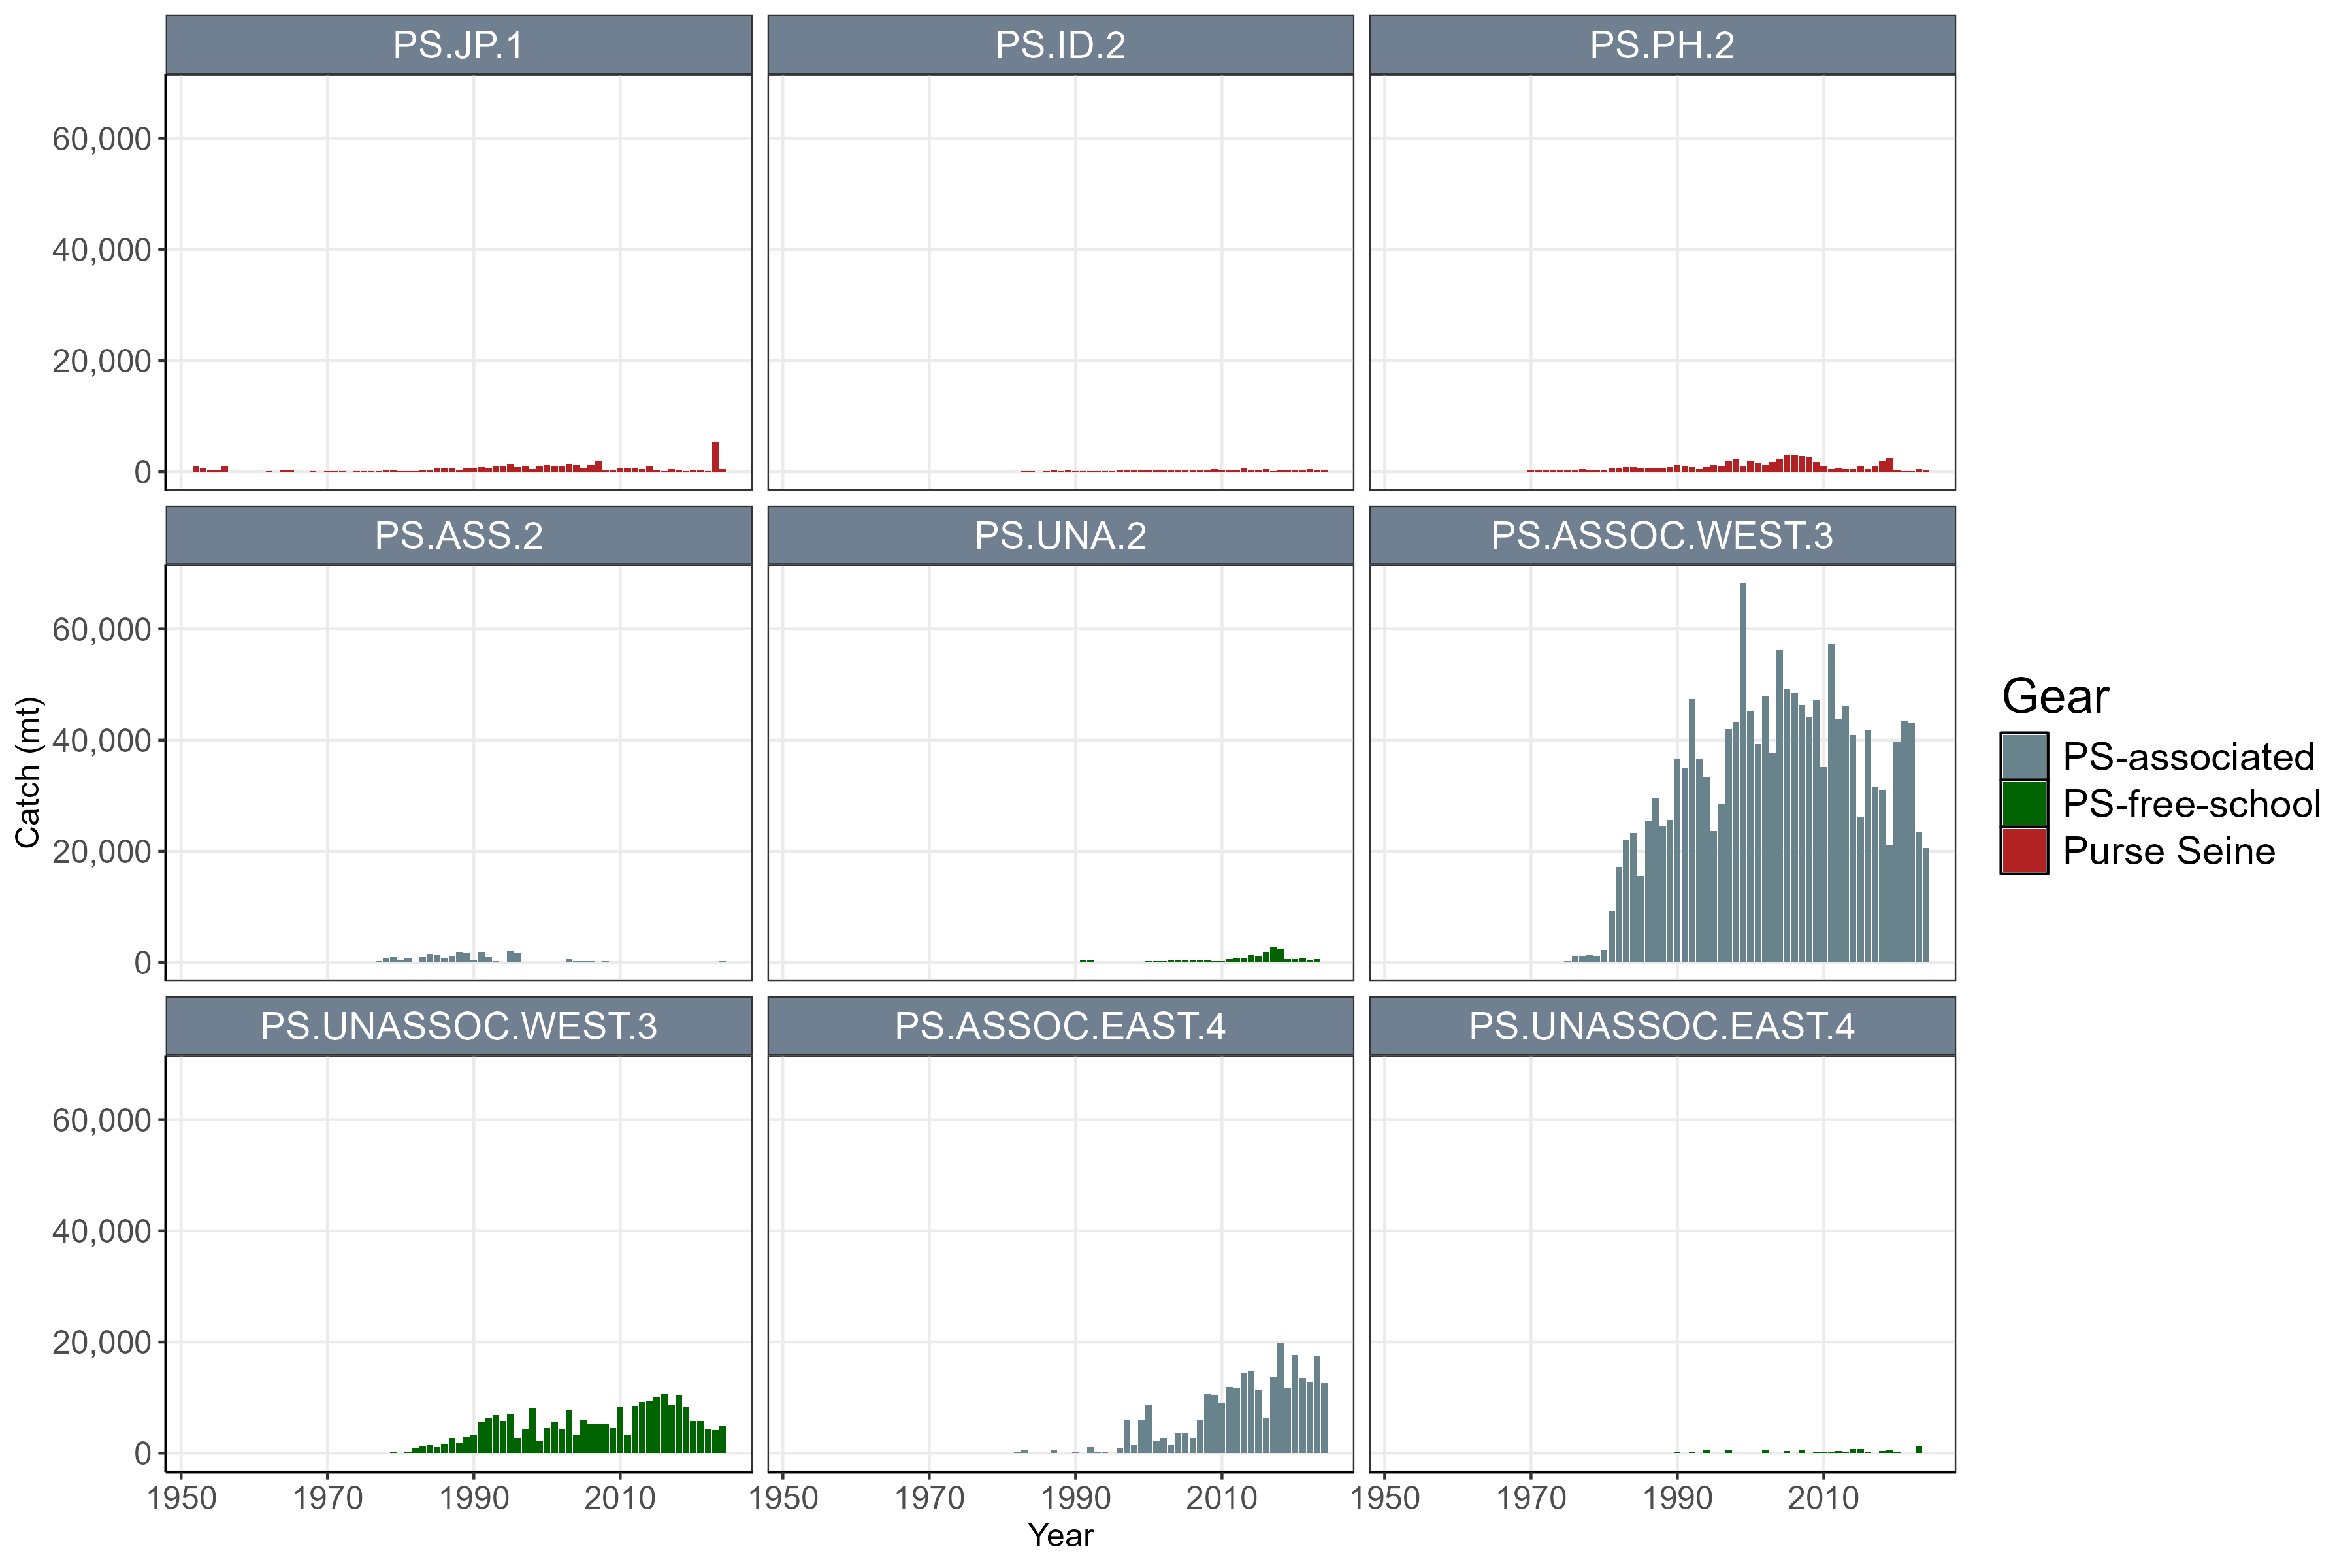
\includegraphics[width=1\linewidth,height=\textheight,keepaspectratio]{figures/catch_by_fishery_ps.png}

}

\caption{\label{fig-catch-by-fishery-ps}Time series of catches (mt) by
fishery: purse seine.}

\end{figure}%

\begin{figure}[H]

\centering{

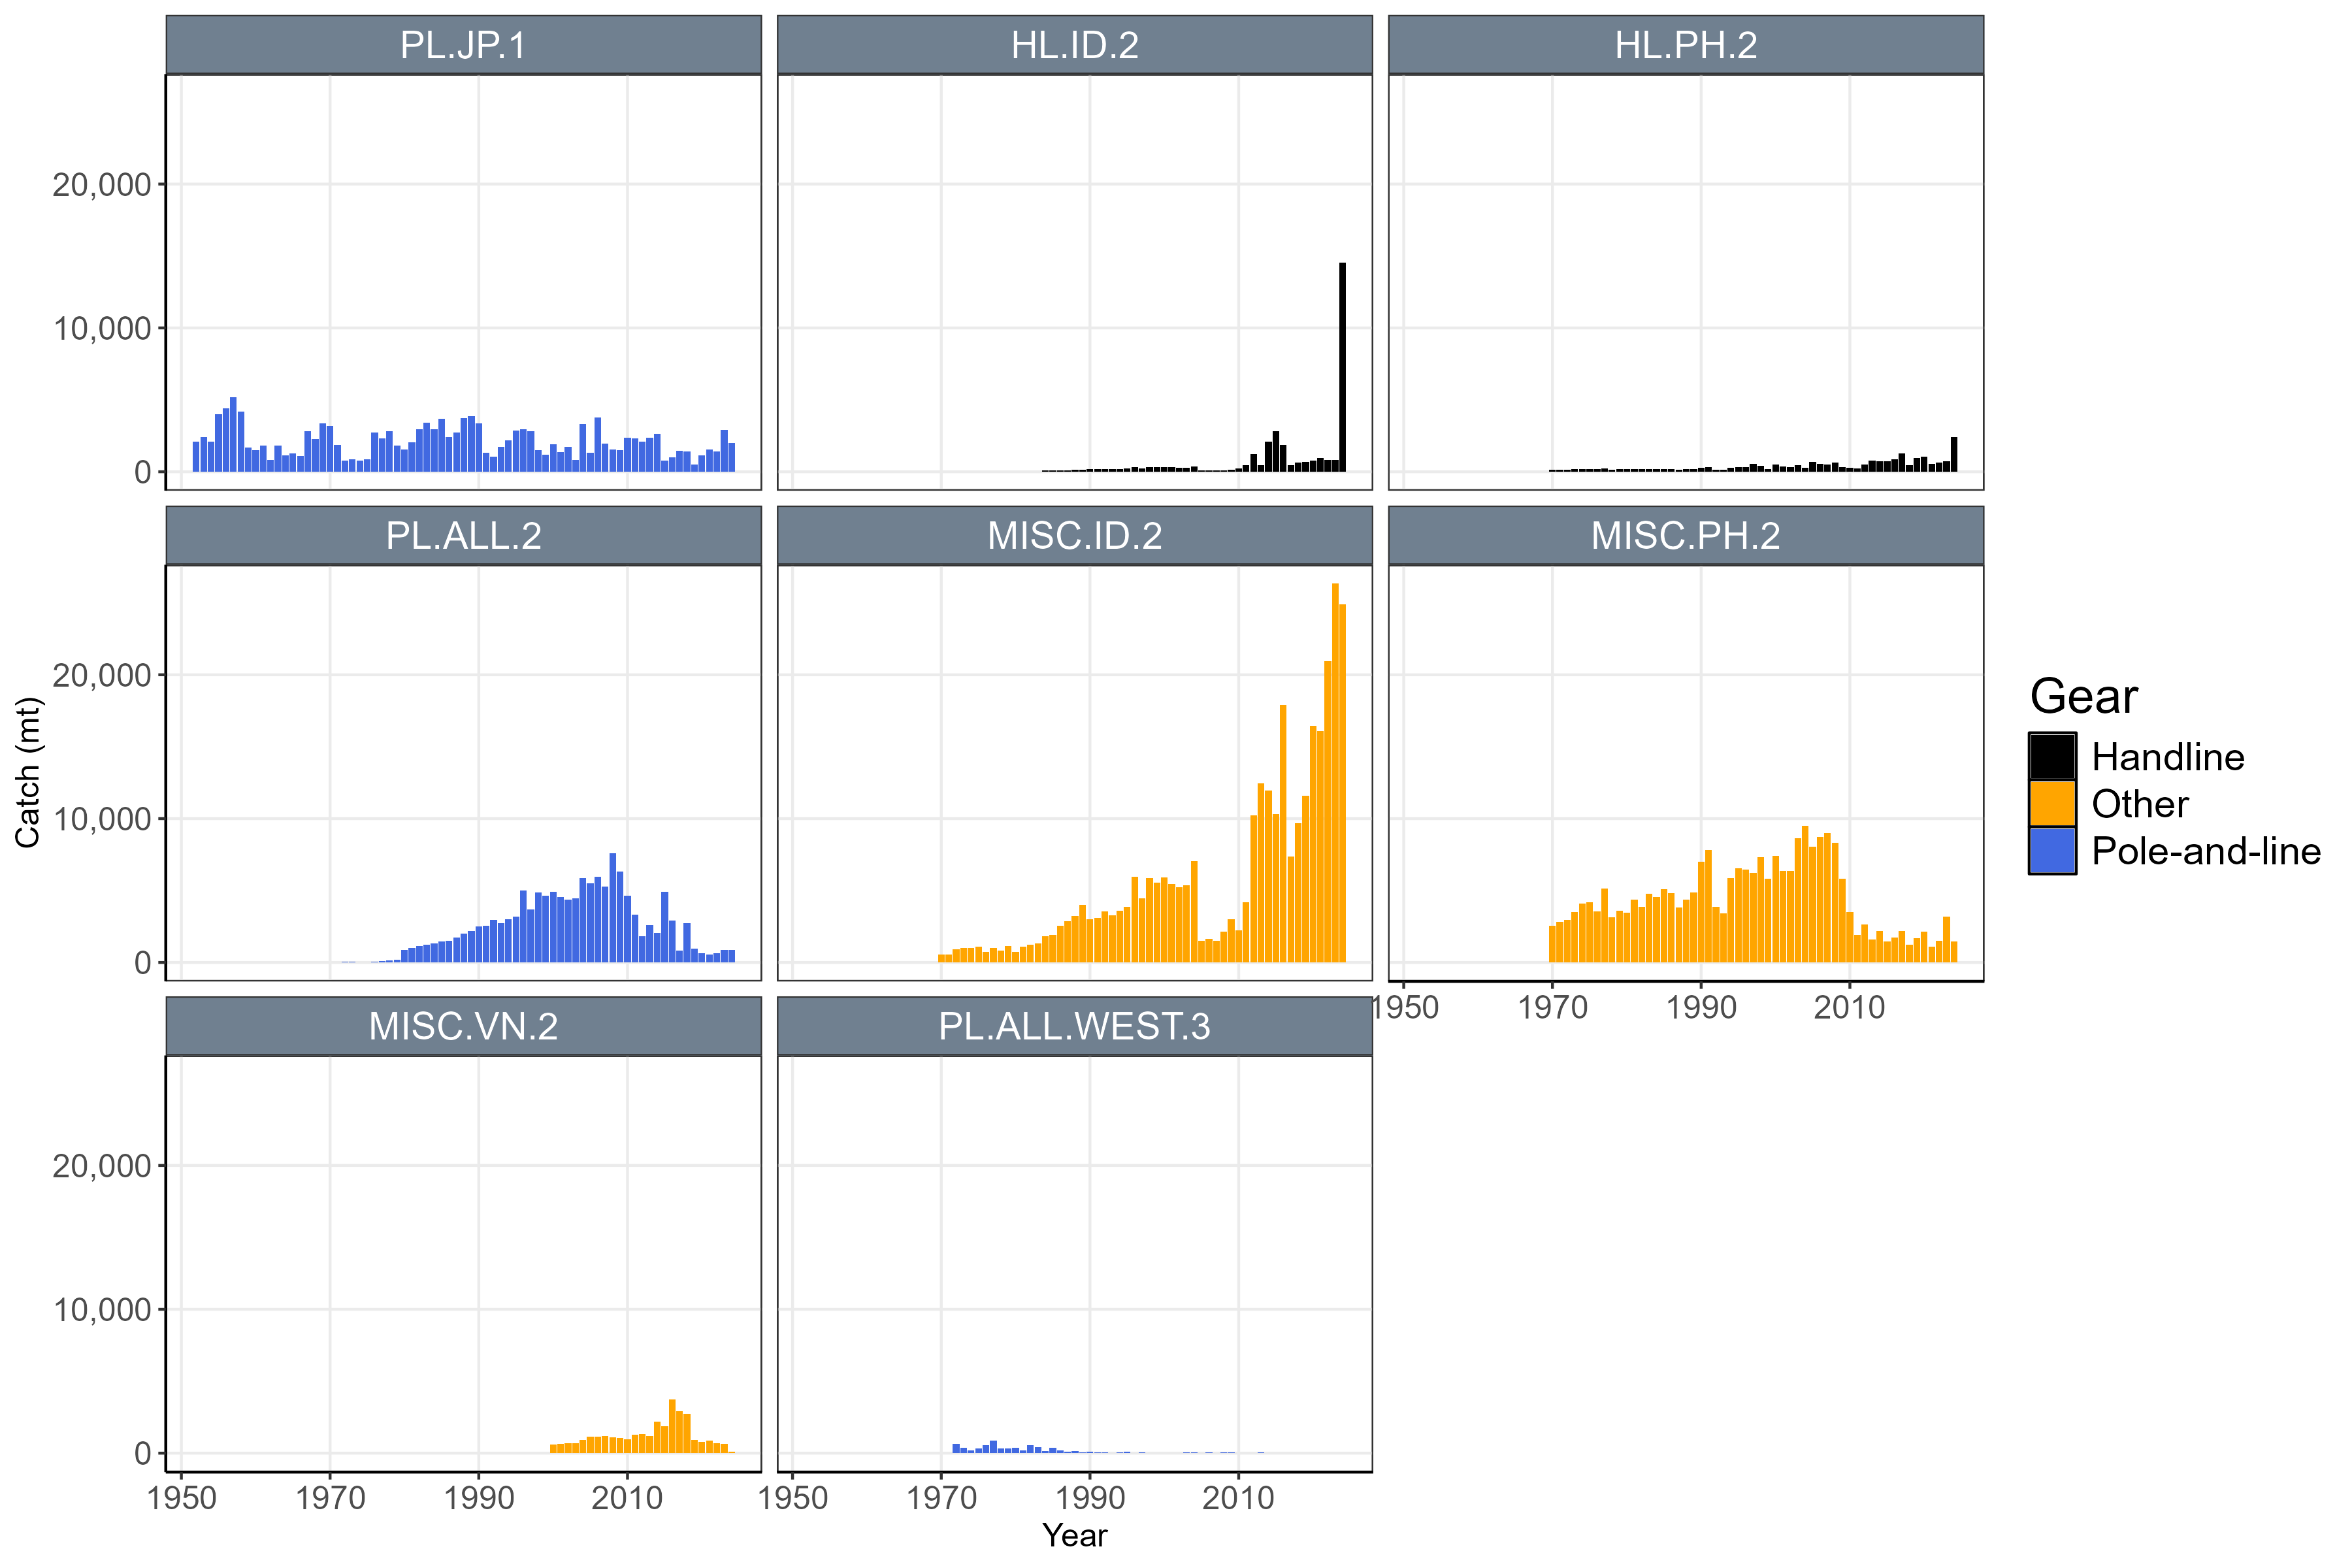
\includegraphics[width=1\linewidth,height=\textheight,keepaspectratio]{figures/catch_by_fishery_other.png}

}

\caption{\label{fig-catch-by-fishery-other}Time series of catches (mt)
by fishery: other.}

\end{figure}%

\begin{figure}[H]

\centering{

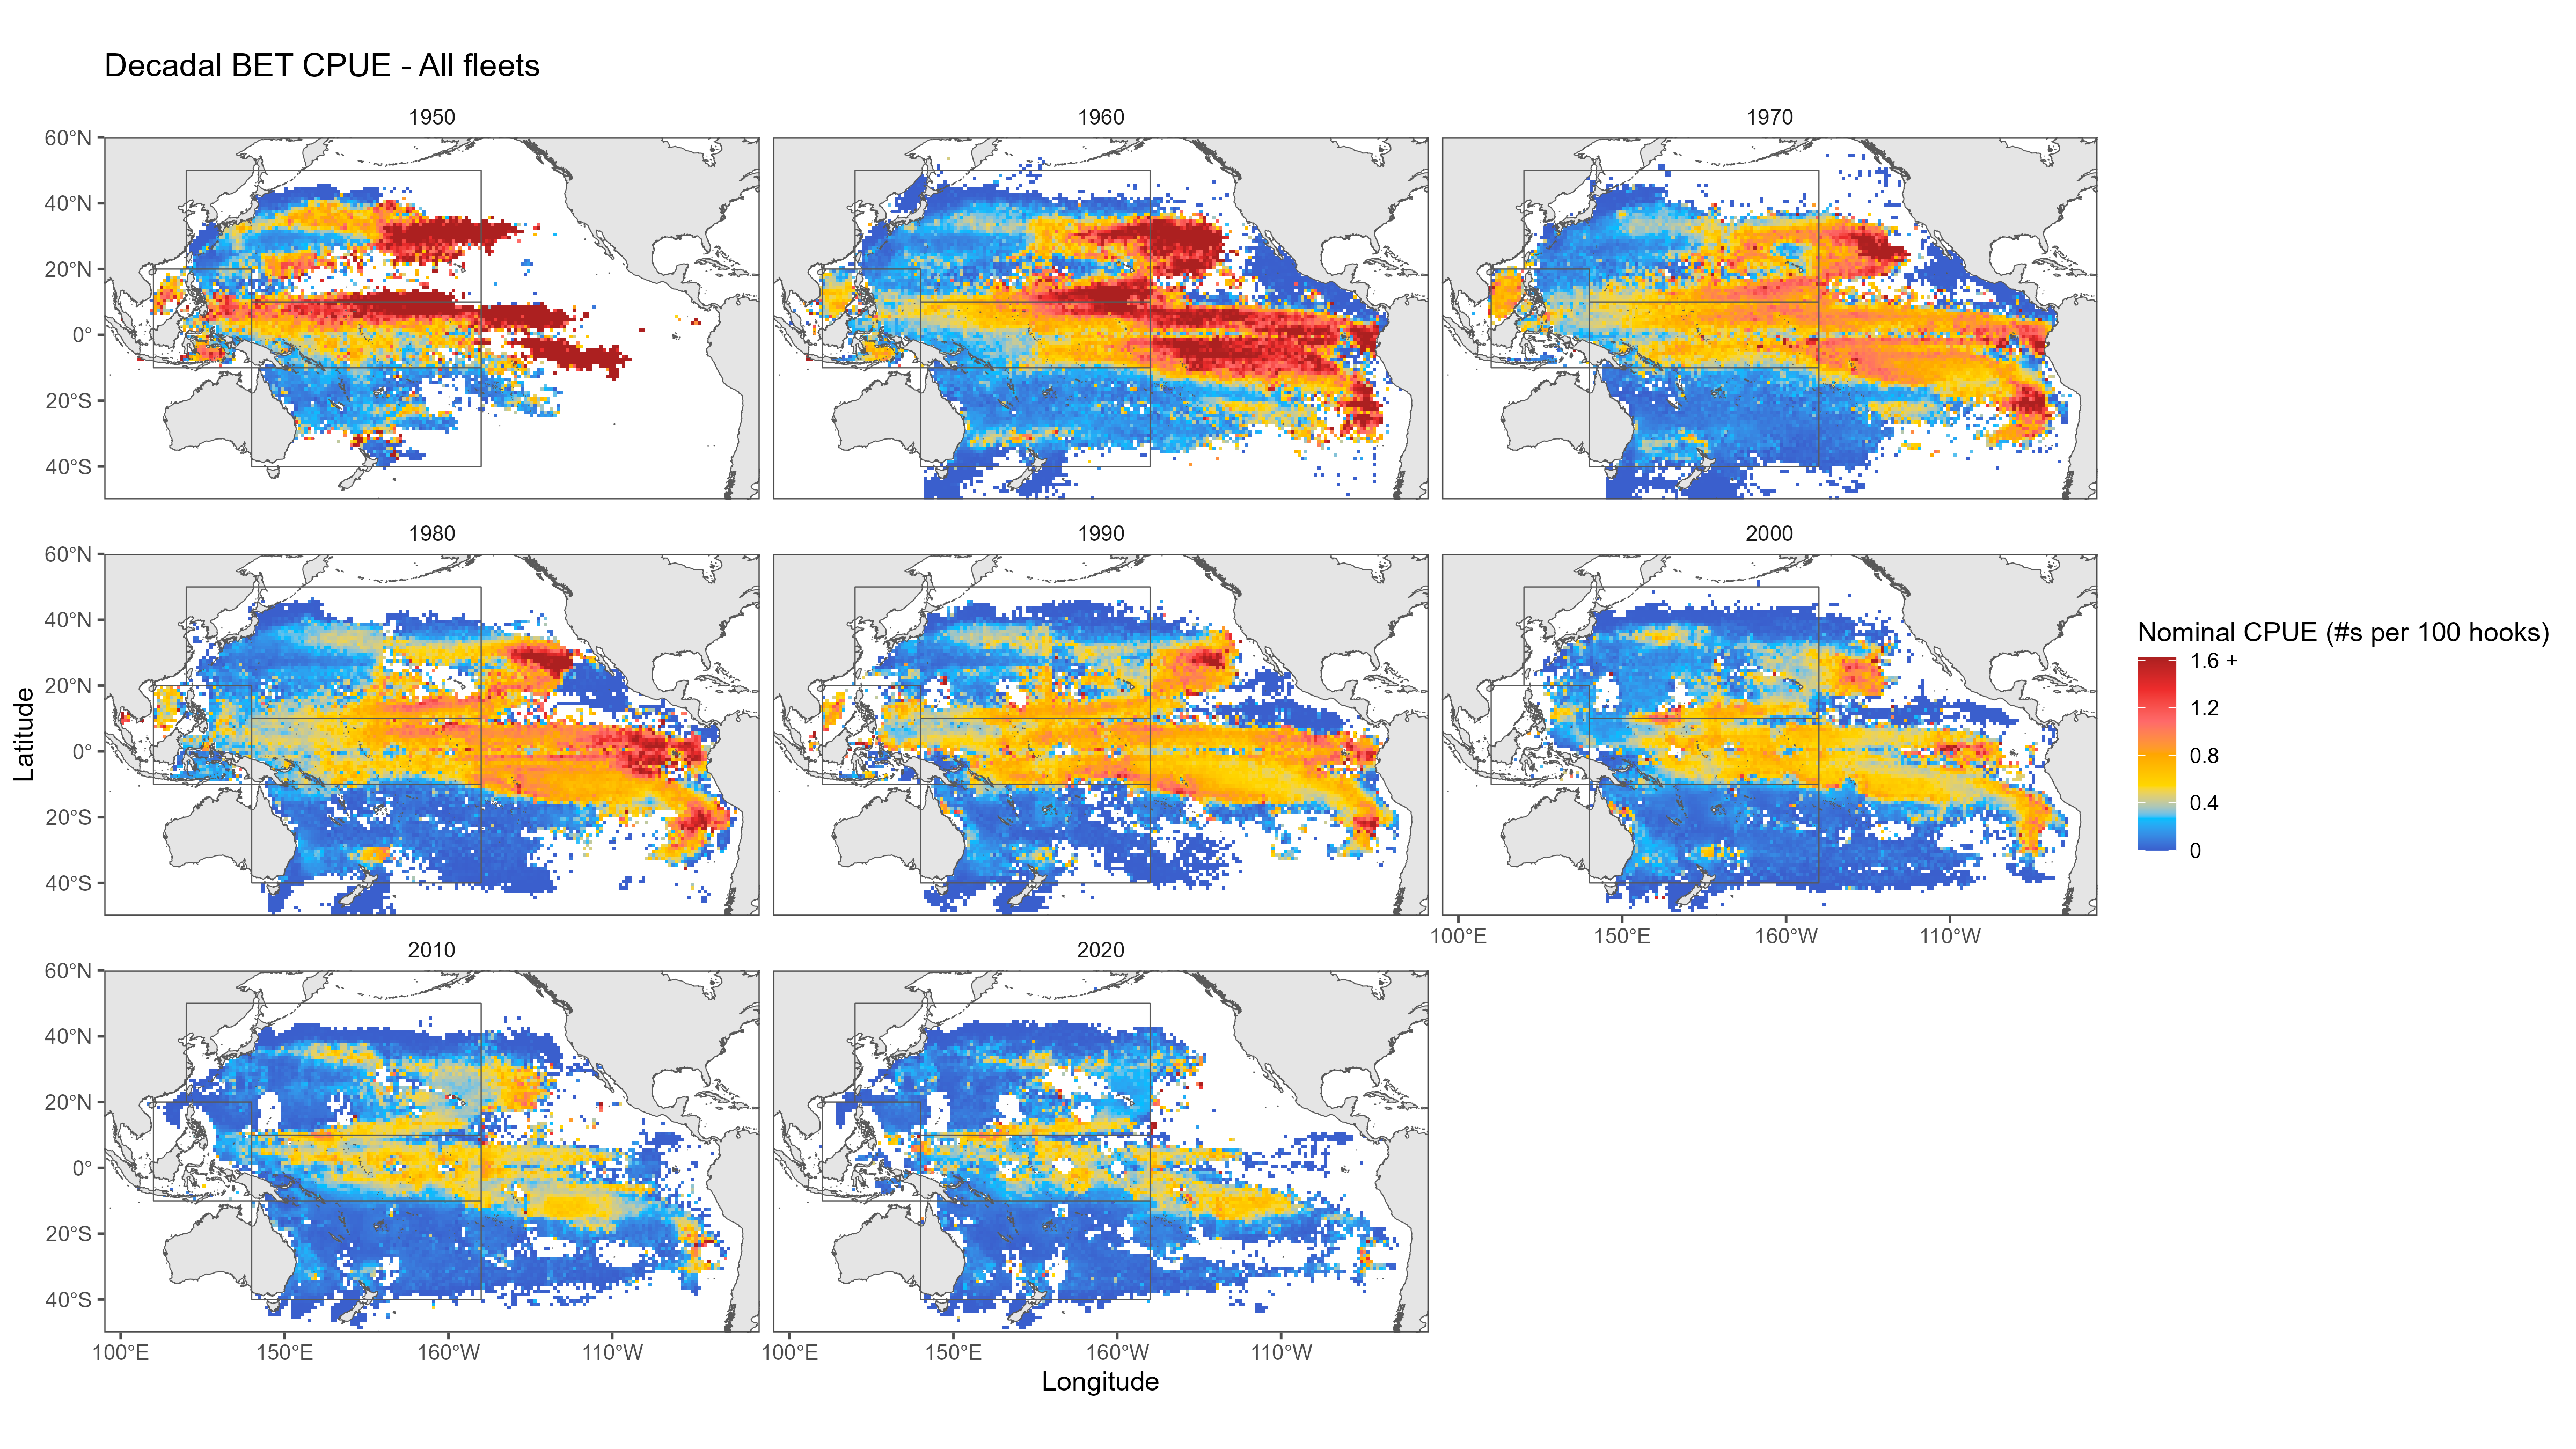
\includegraphics[width=1\linewidth,height=\textheight,keepaspectratio]{figures/cpue_nom_maps.png}

}

\caption{\label{fig-cpue-nom-maps}Spatial distribution of nominal
longline CPUE (all fleets) for bigeye in the Pacific.}

\end{figure}%

\begin{figure}[H]

\centering{

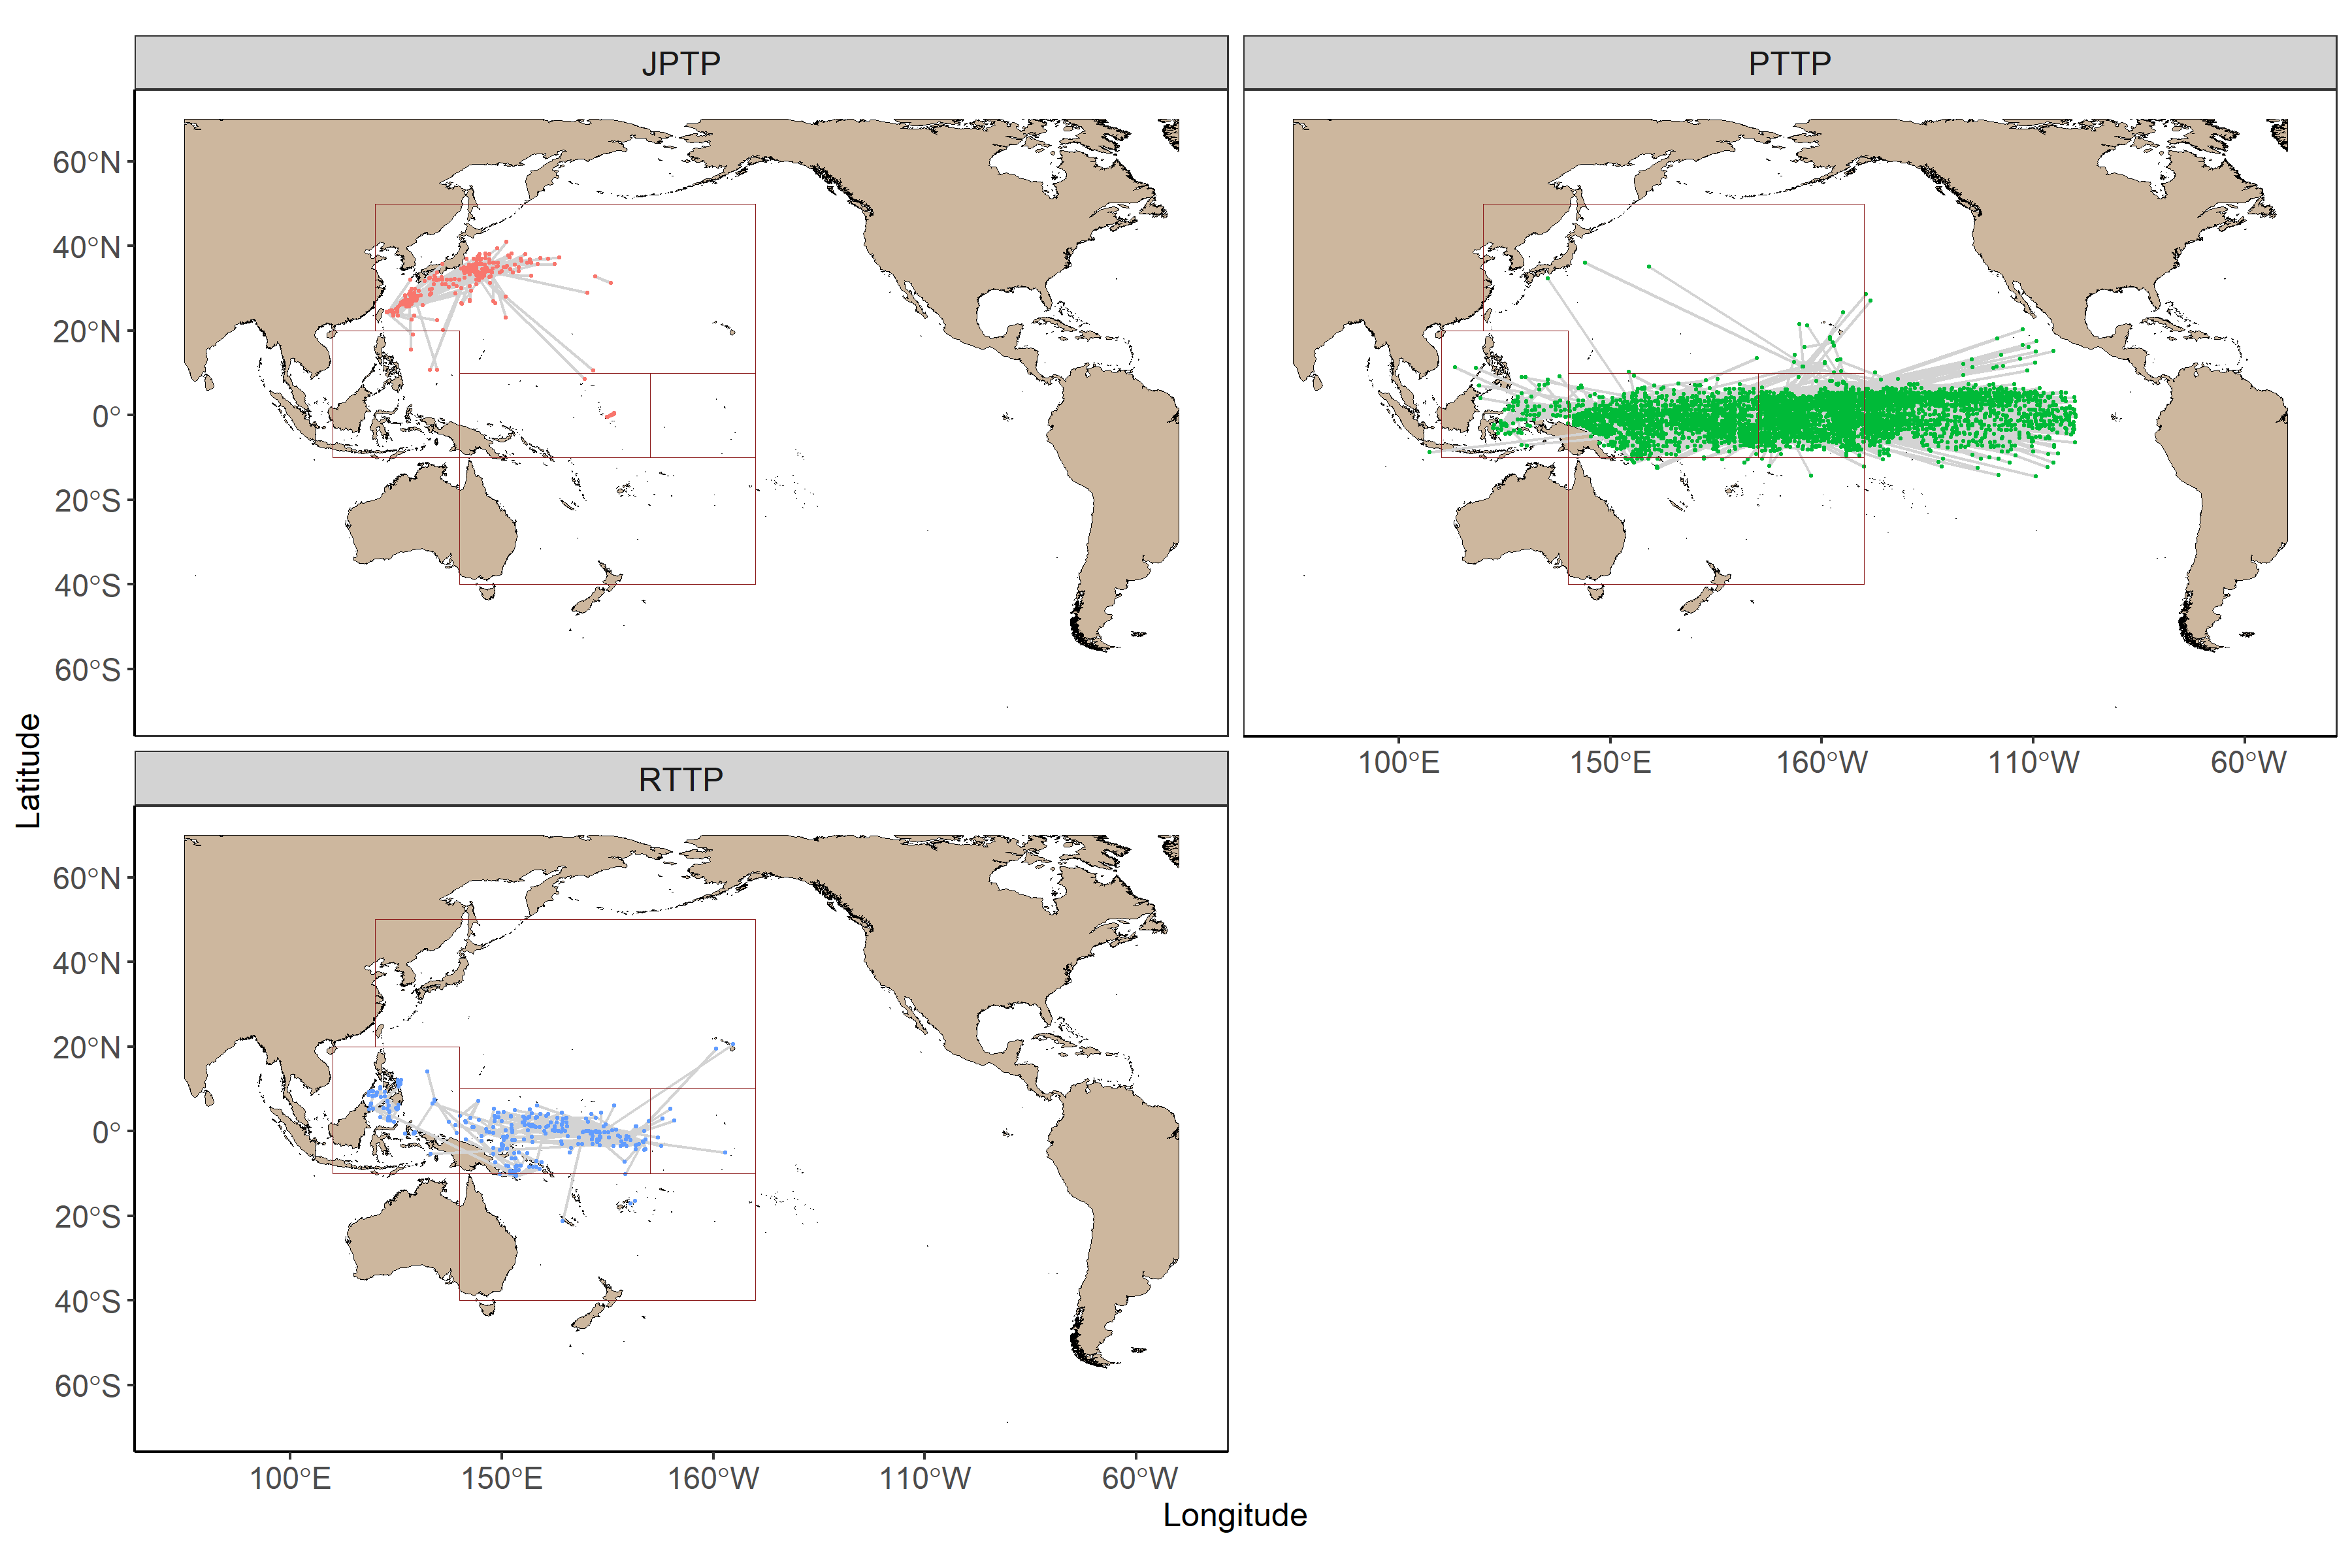
\includegraphics[width=1\linewidth,height=\textheight,keepaspectratio]{figures/tag_displacement_map.png}

}

\caption{\label{fig-tag-displacement-map}Map of tag recaptures. The
panel shows the distributions of release and recapture displacements for
the different tagging programs. Pacific Tuna Tagging Program (PTTP),
Regional Tuna Tagging Program (excluding Coral Sea tags) (RTTP) and the
Japanese Tagging Program (JPTP). Dots indicate recapture locations.}

\end{figure}%

\begin{figure}[H]

\centering{

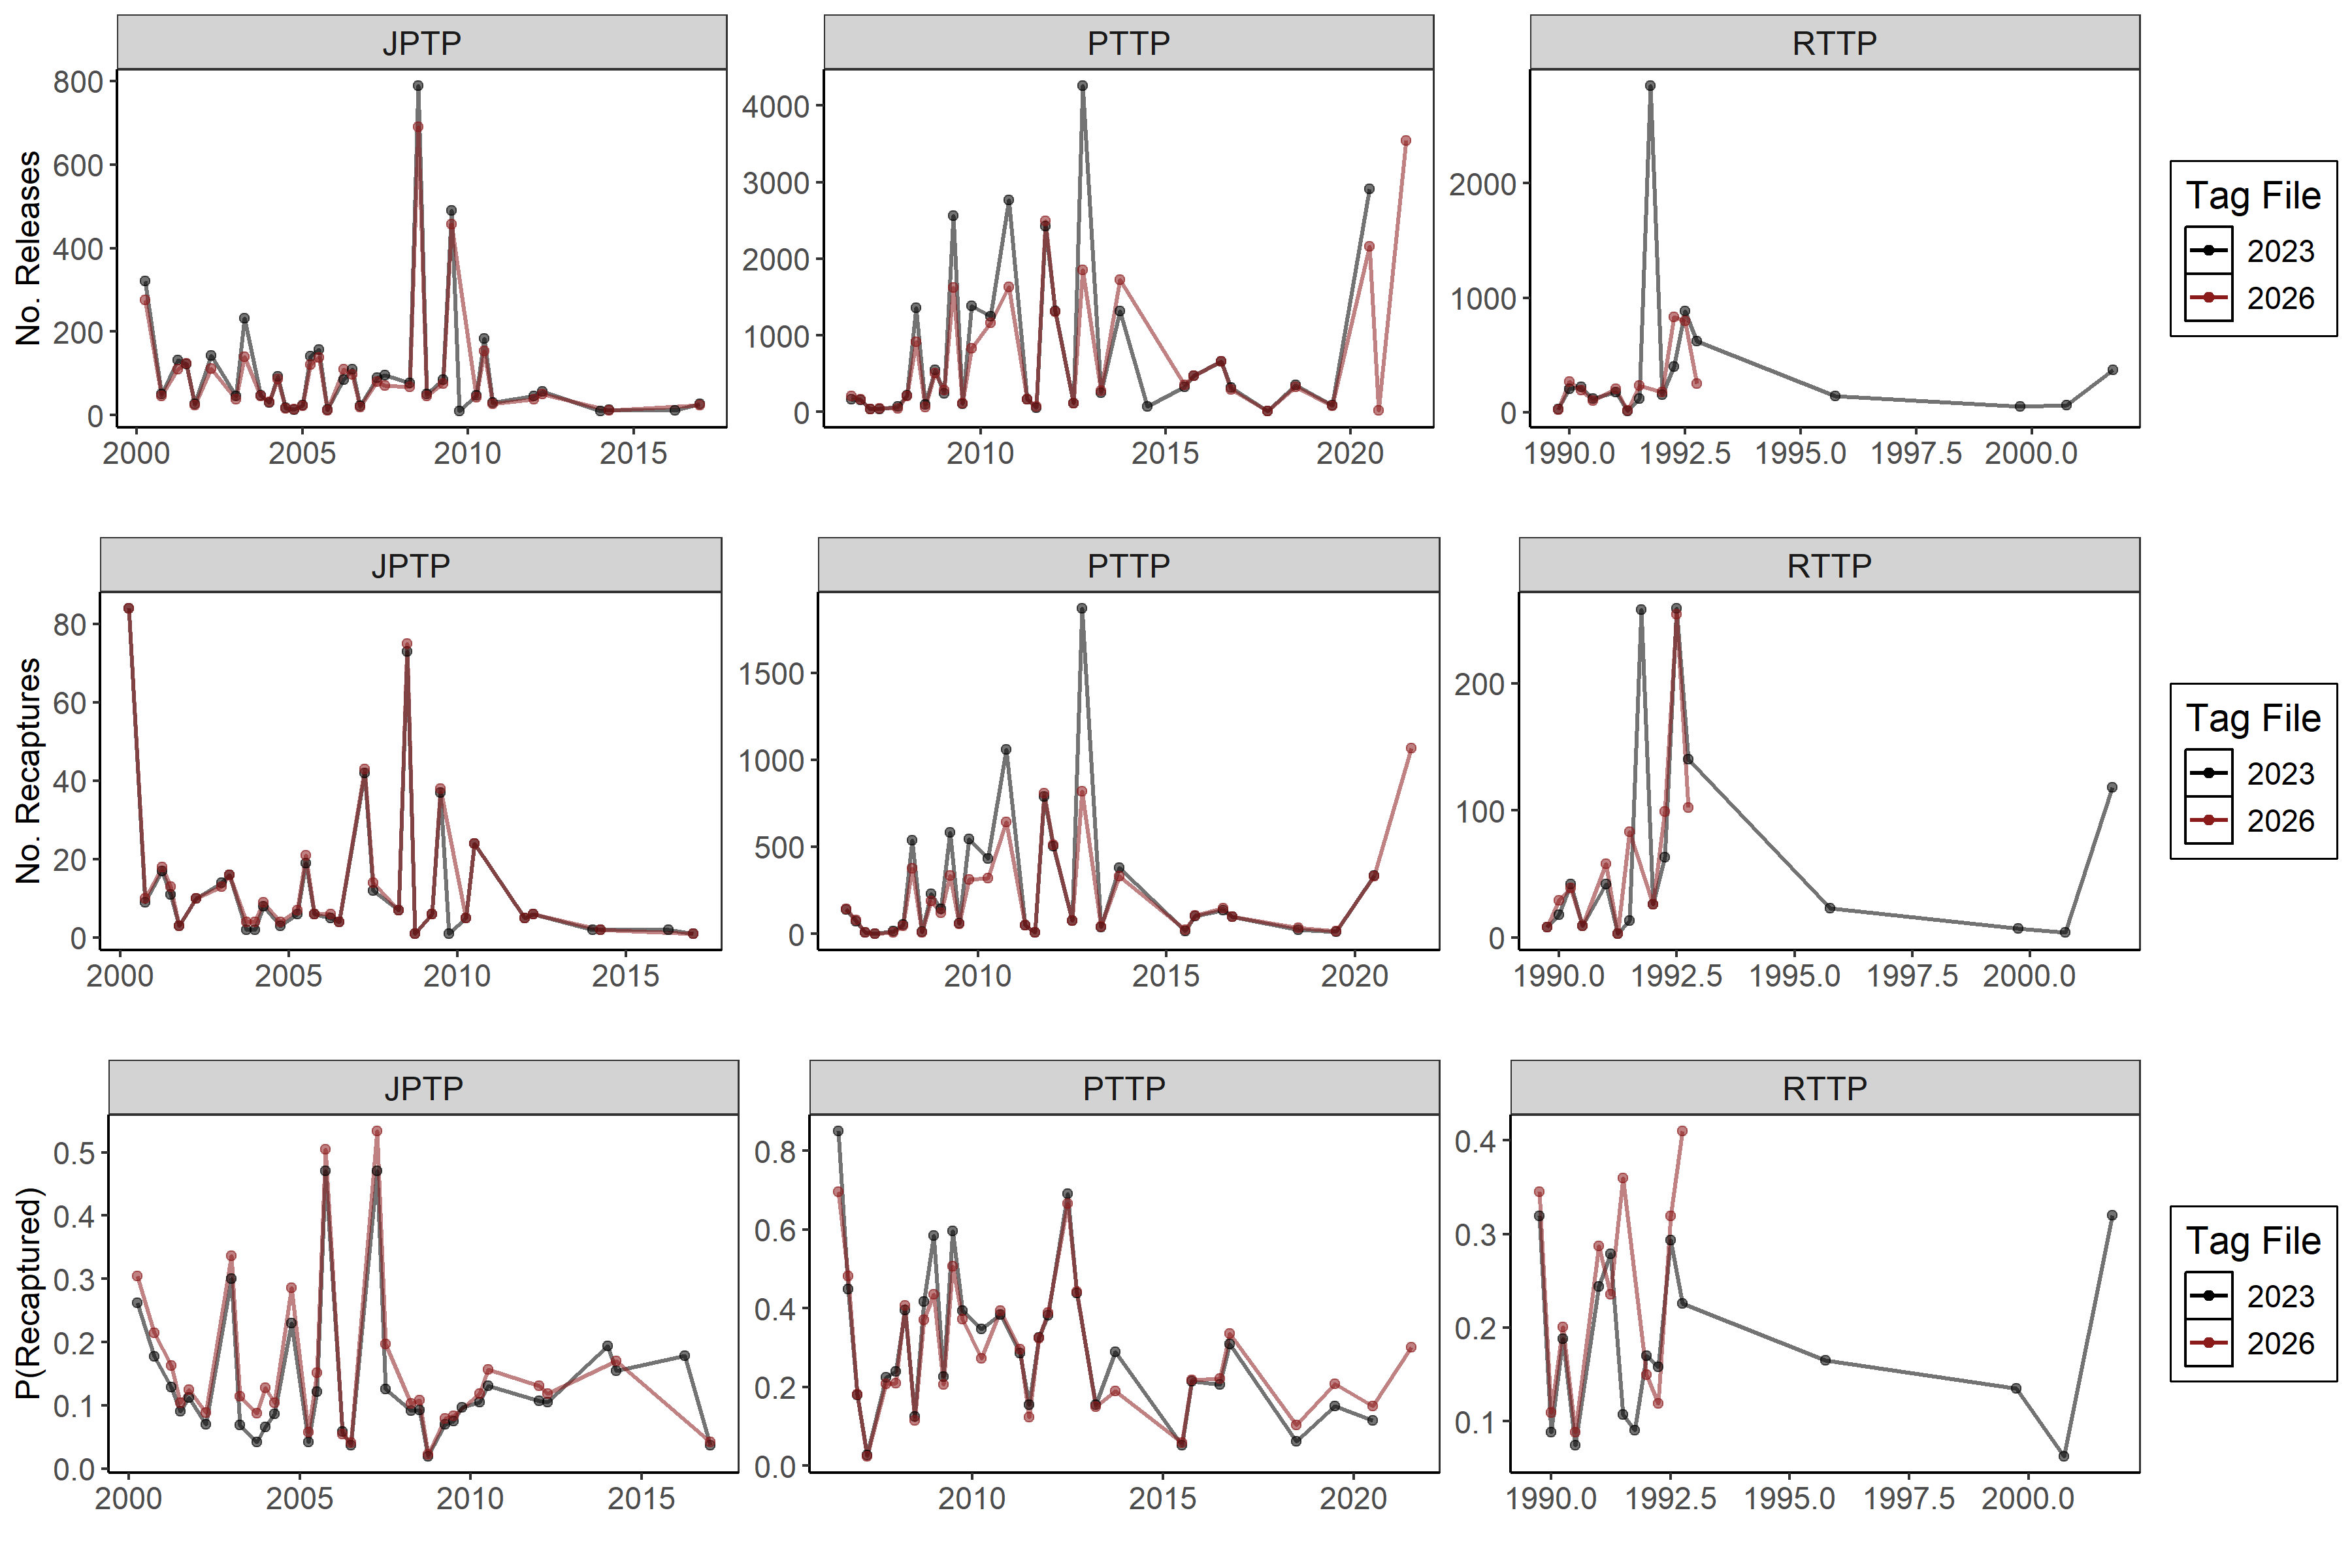
\includegraphics[width=1\linewidth,height=\textheight,keepaspectratio]{figures/tag_release_recapt.png}

}

\caption{\label{fig-tag-release-recapt}Summary plots of the number of
releases, recaptures, and recapture rate of tags, by tagging program and
region.}

\end{figure}%

\DIFdelbegin %DIFDELCMD < \begin{figure}[H]
%DIFDELCMD <

%DIFDELCMD < \centering{
%DIFDELCMD <

%DIFDELCMD < 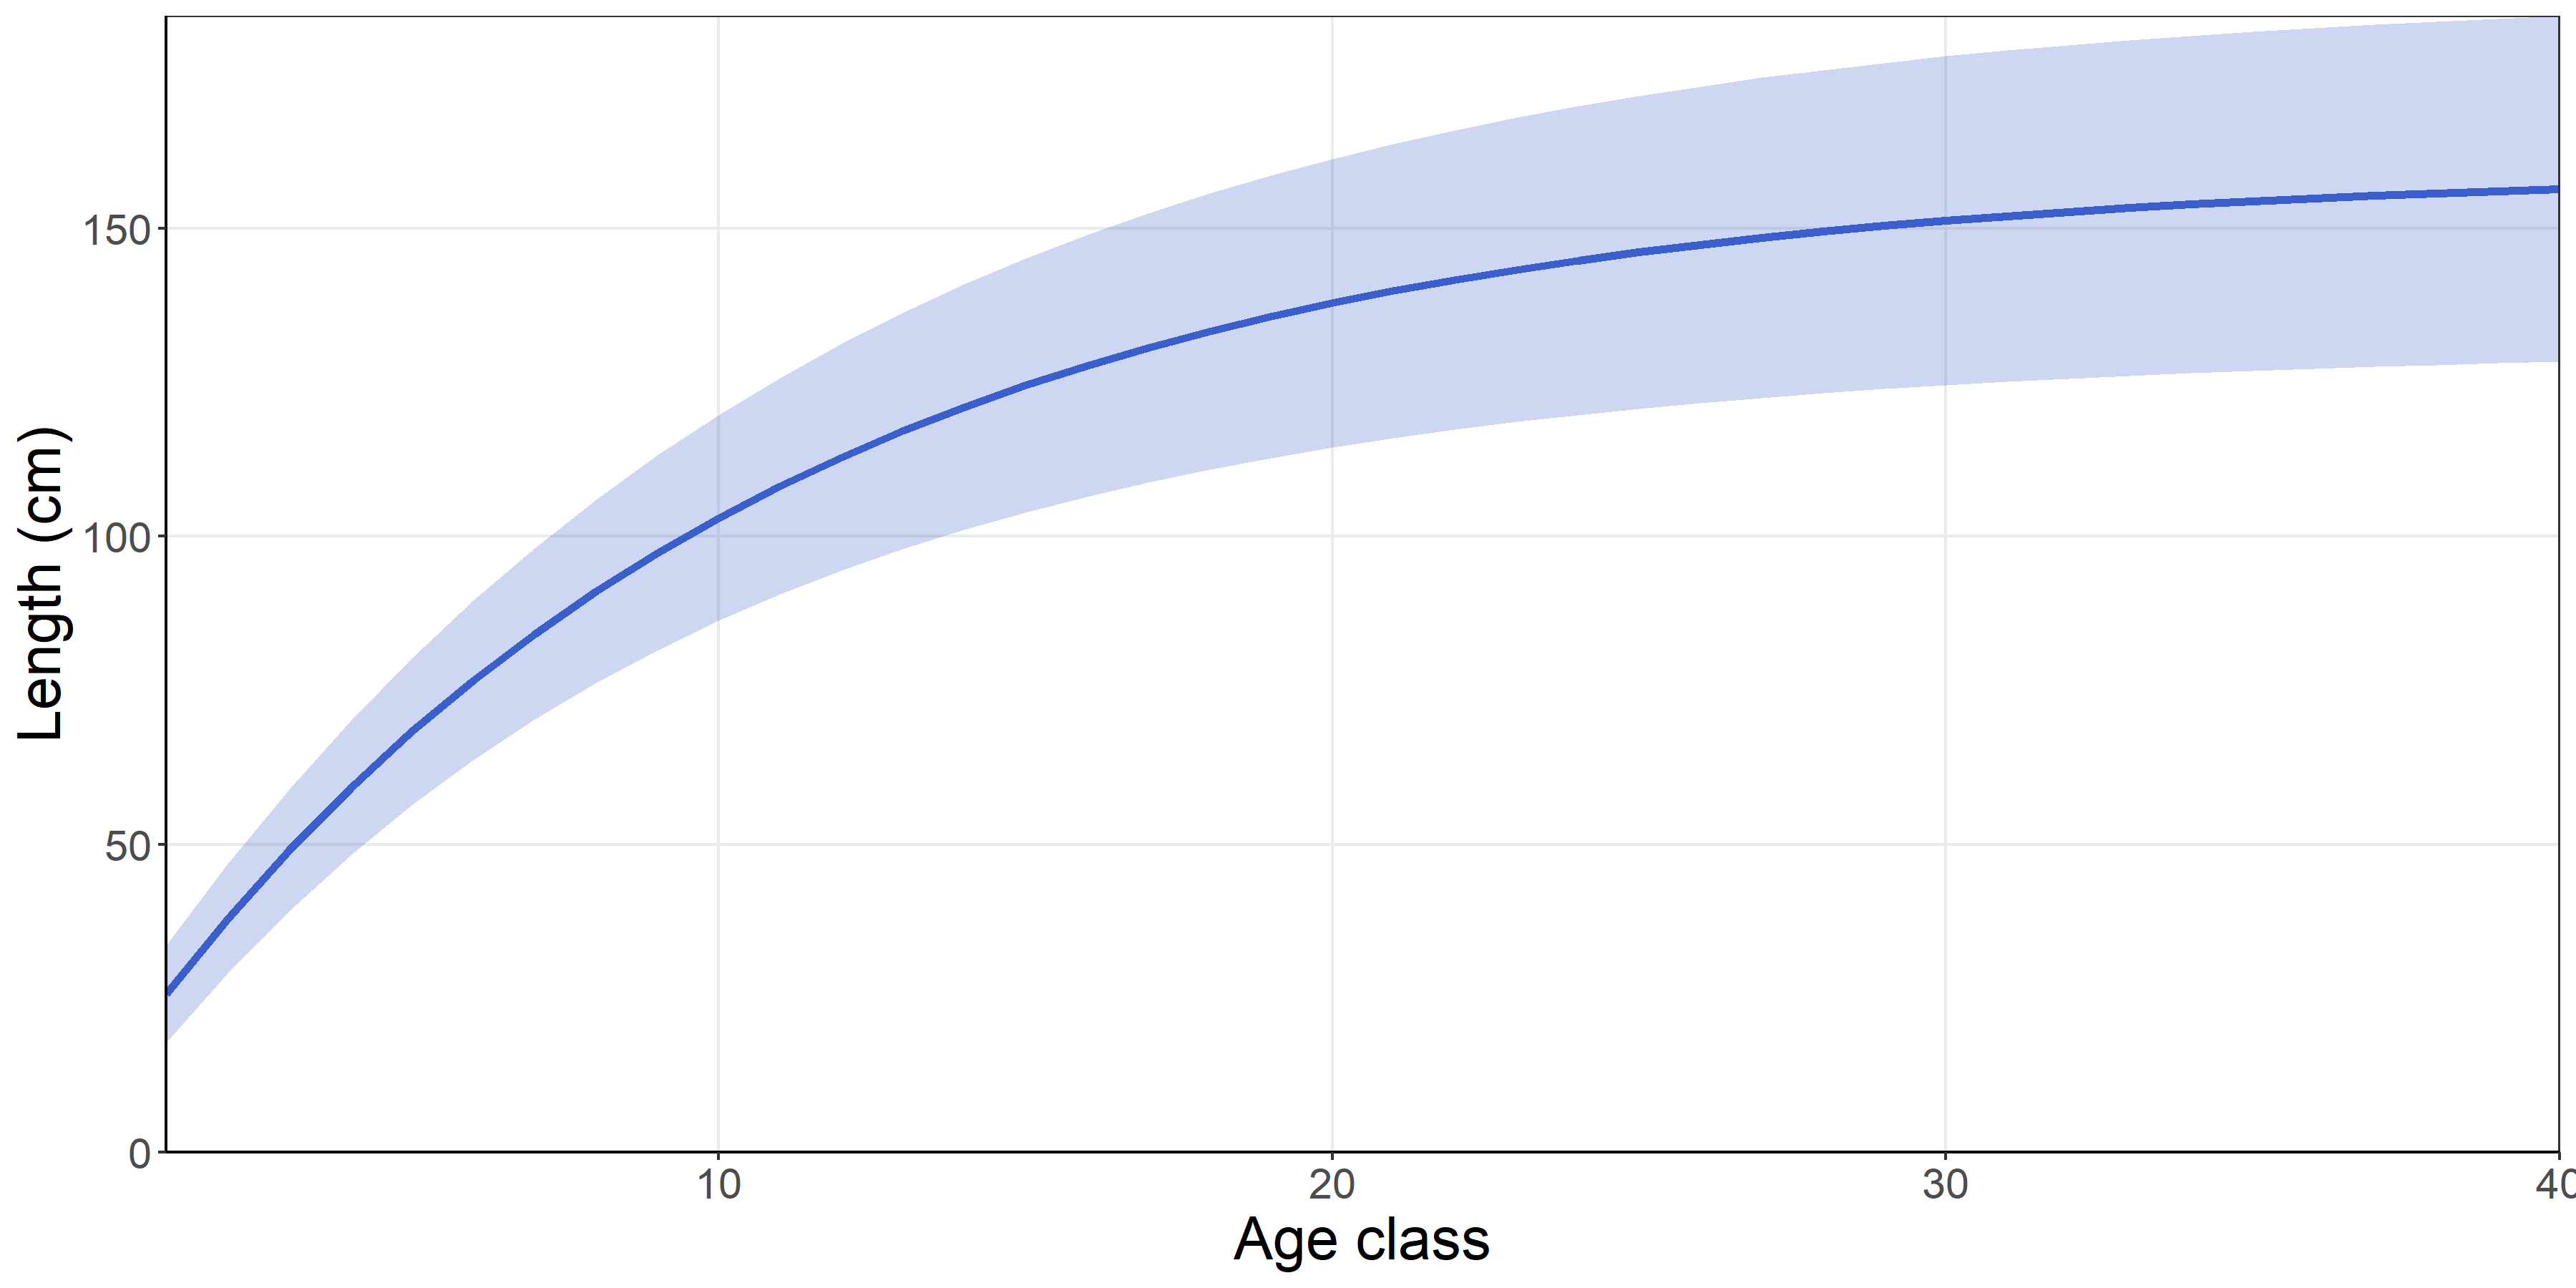
\includegraphics[width=1\linewidth,height=\textheight,keepaspectratio]{figures/growth_curve.png}
%DIFDELCMD <

%DIFDELCMD < }
%DIFDELCMD <

%DIFDELCMD < \caption{\label{fig-growth-curve}Estimated growth curve for the 2026
%DIFDELCMD < diagnostic model.}
%DIFDELCMD <

%DIFDELCMD < \end{figure}%%%
\DIFdelend \DIFaddbegin \begin{figure}[H]

\centering{

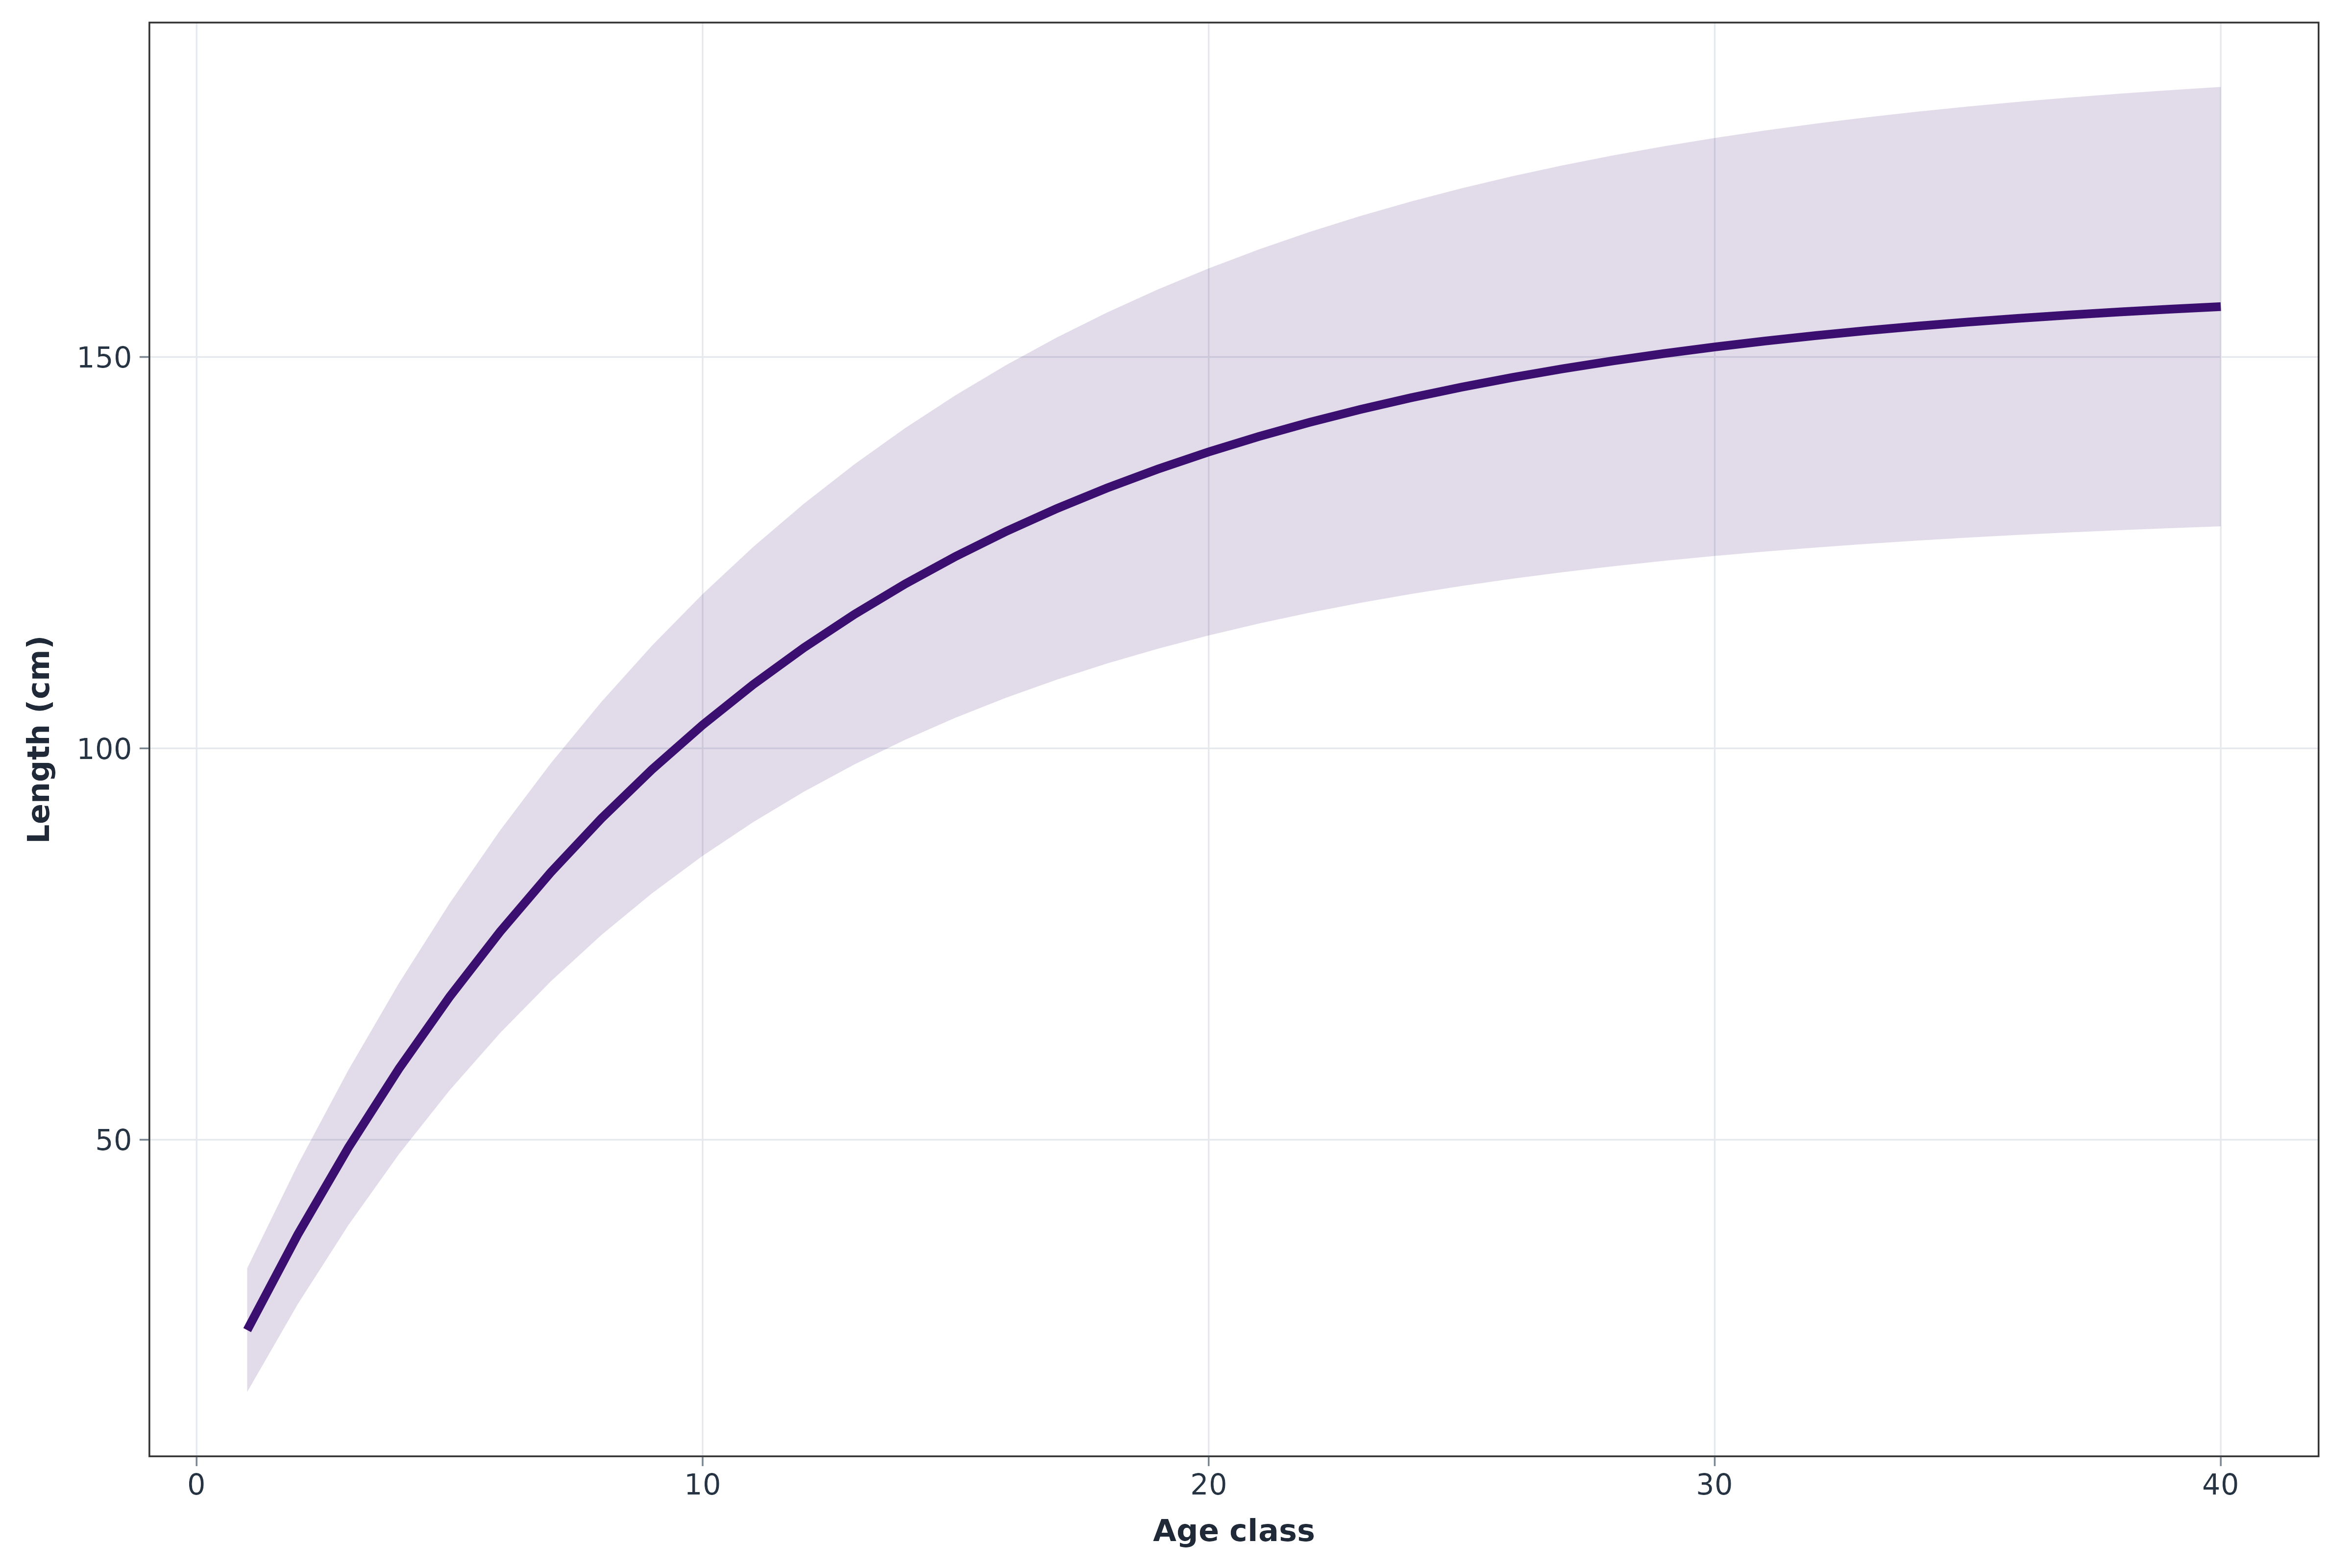
\includegraphics[width=1\linewidth,height=\textheight,keepaspectratio]{figures_new/growth-curve.png}

}

\caption{\label{fig-growth-curve}Fitted mean length at age for the 2026
diagnostic model. Shading is the mean plus or minus 1.96 length-at-age
standard deviations and represents fish-level length variability, not
parameter-estimation uncertainty.}

\end{figure}\DIFaddend %

\begin{figure}[H]

\centering{

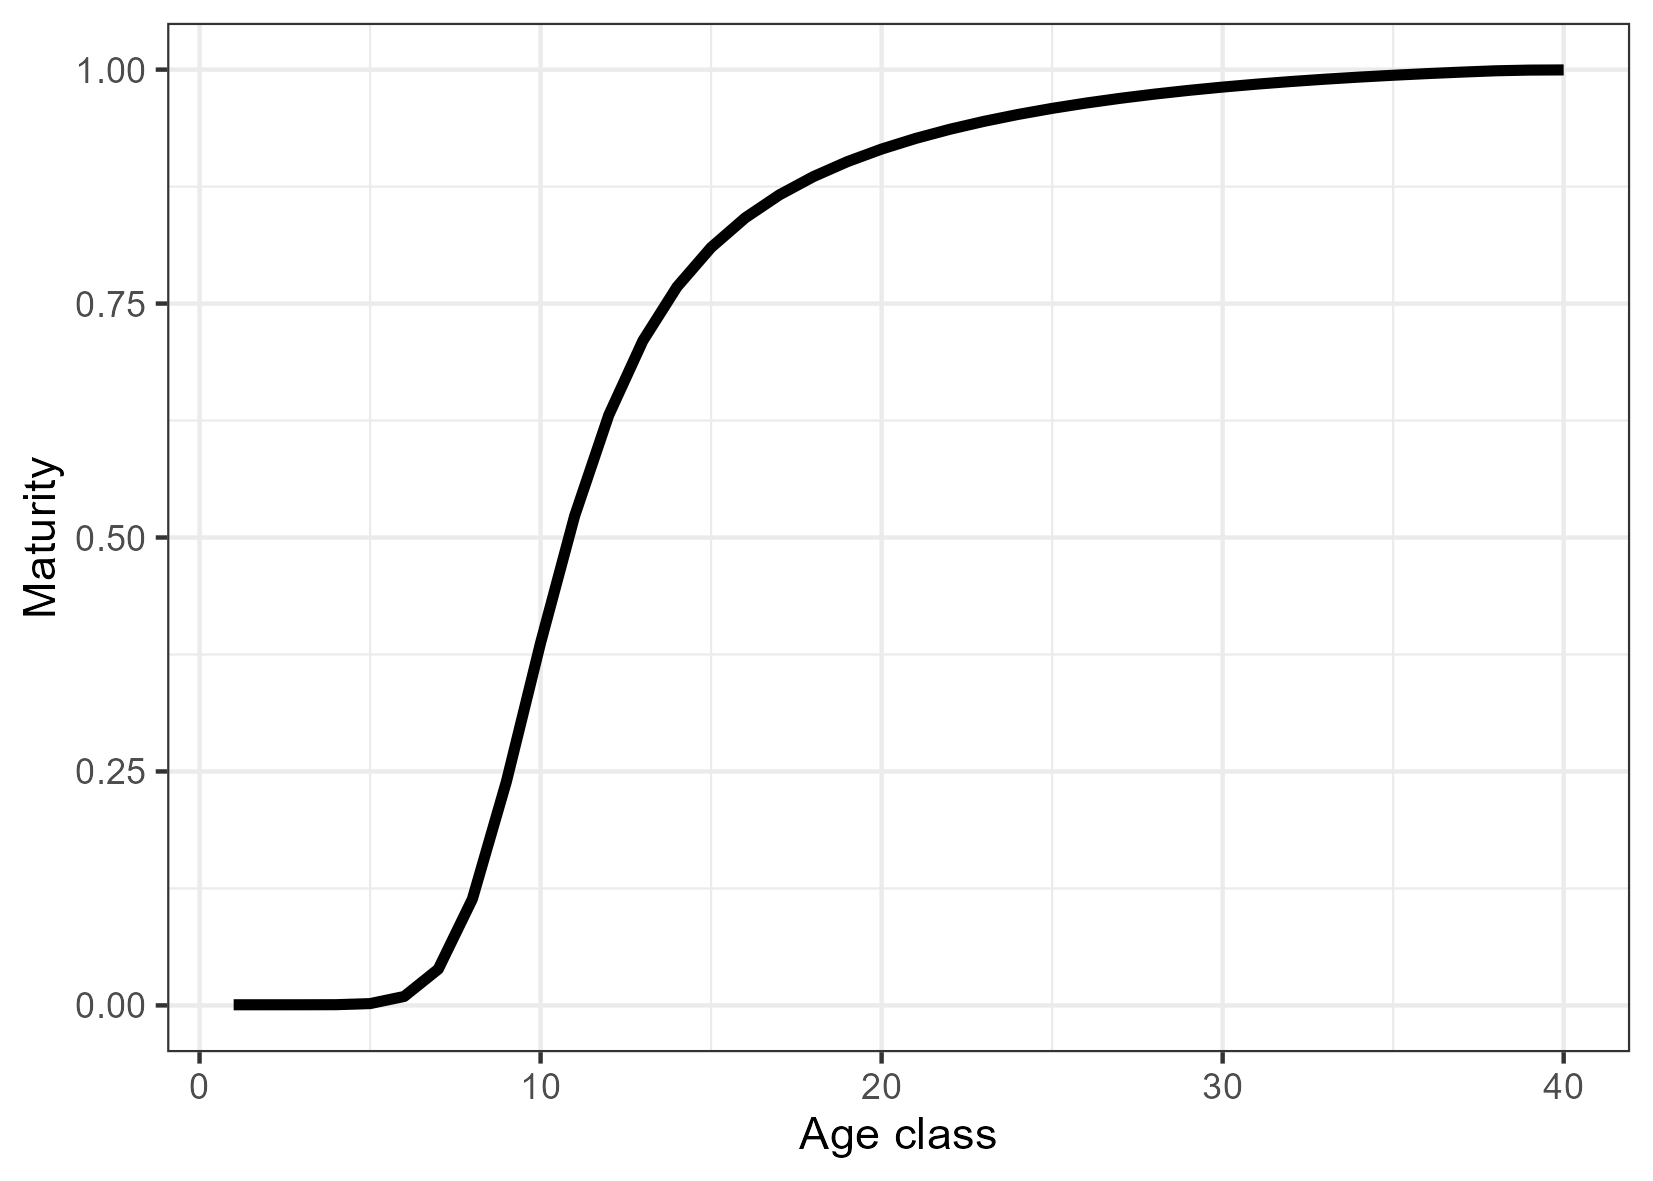
\includegraphics[width=1\linewidth,height=\textheight,keepaspectratio]{figures/maturity_ogive.png}

}

\caption{\label{fig-maturity-ogive}Maturity-at-age ogive for the 2026
diagnostic model.}

\end{figure}%

\begin{figure}[H]

\centering{

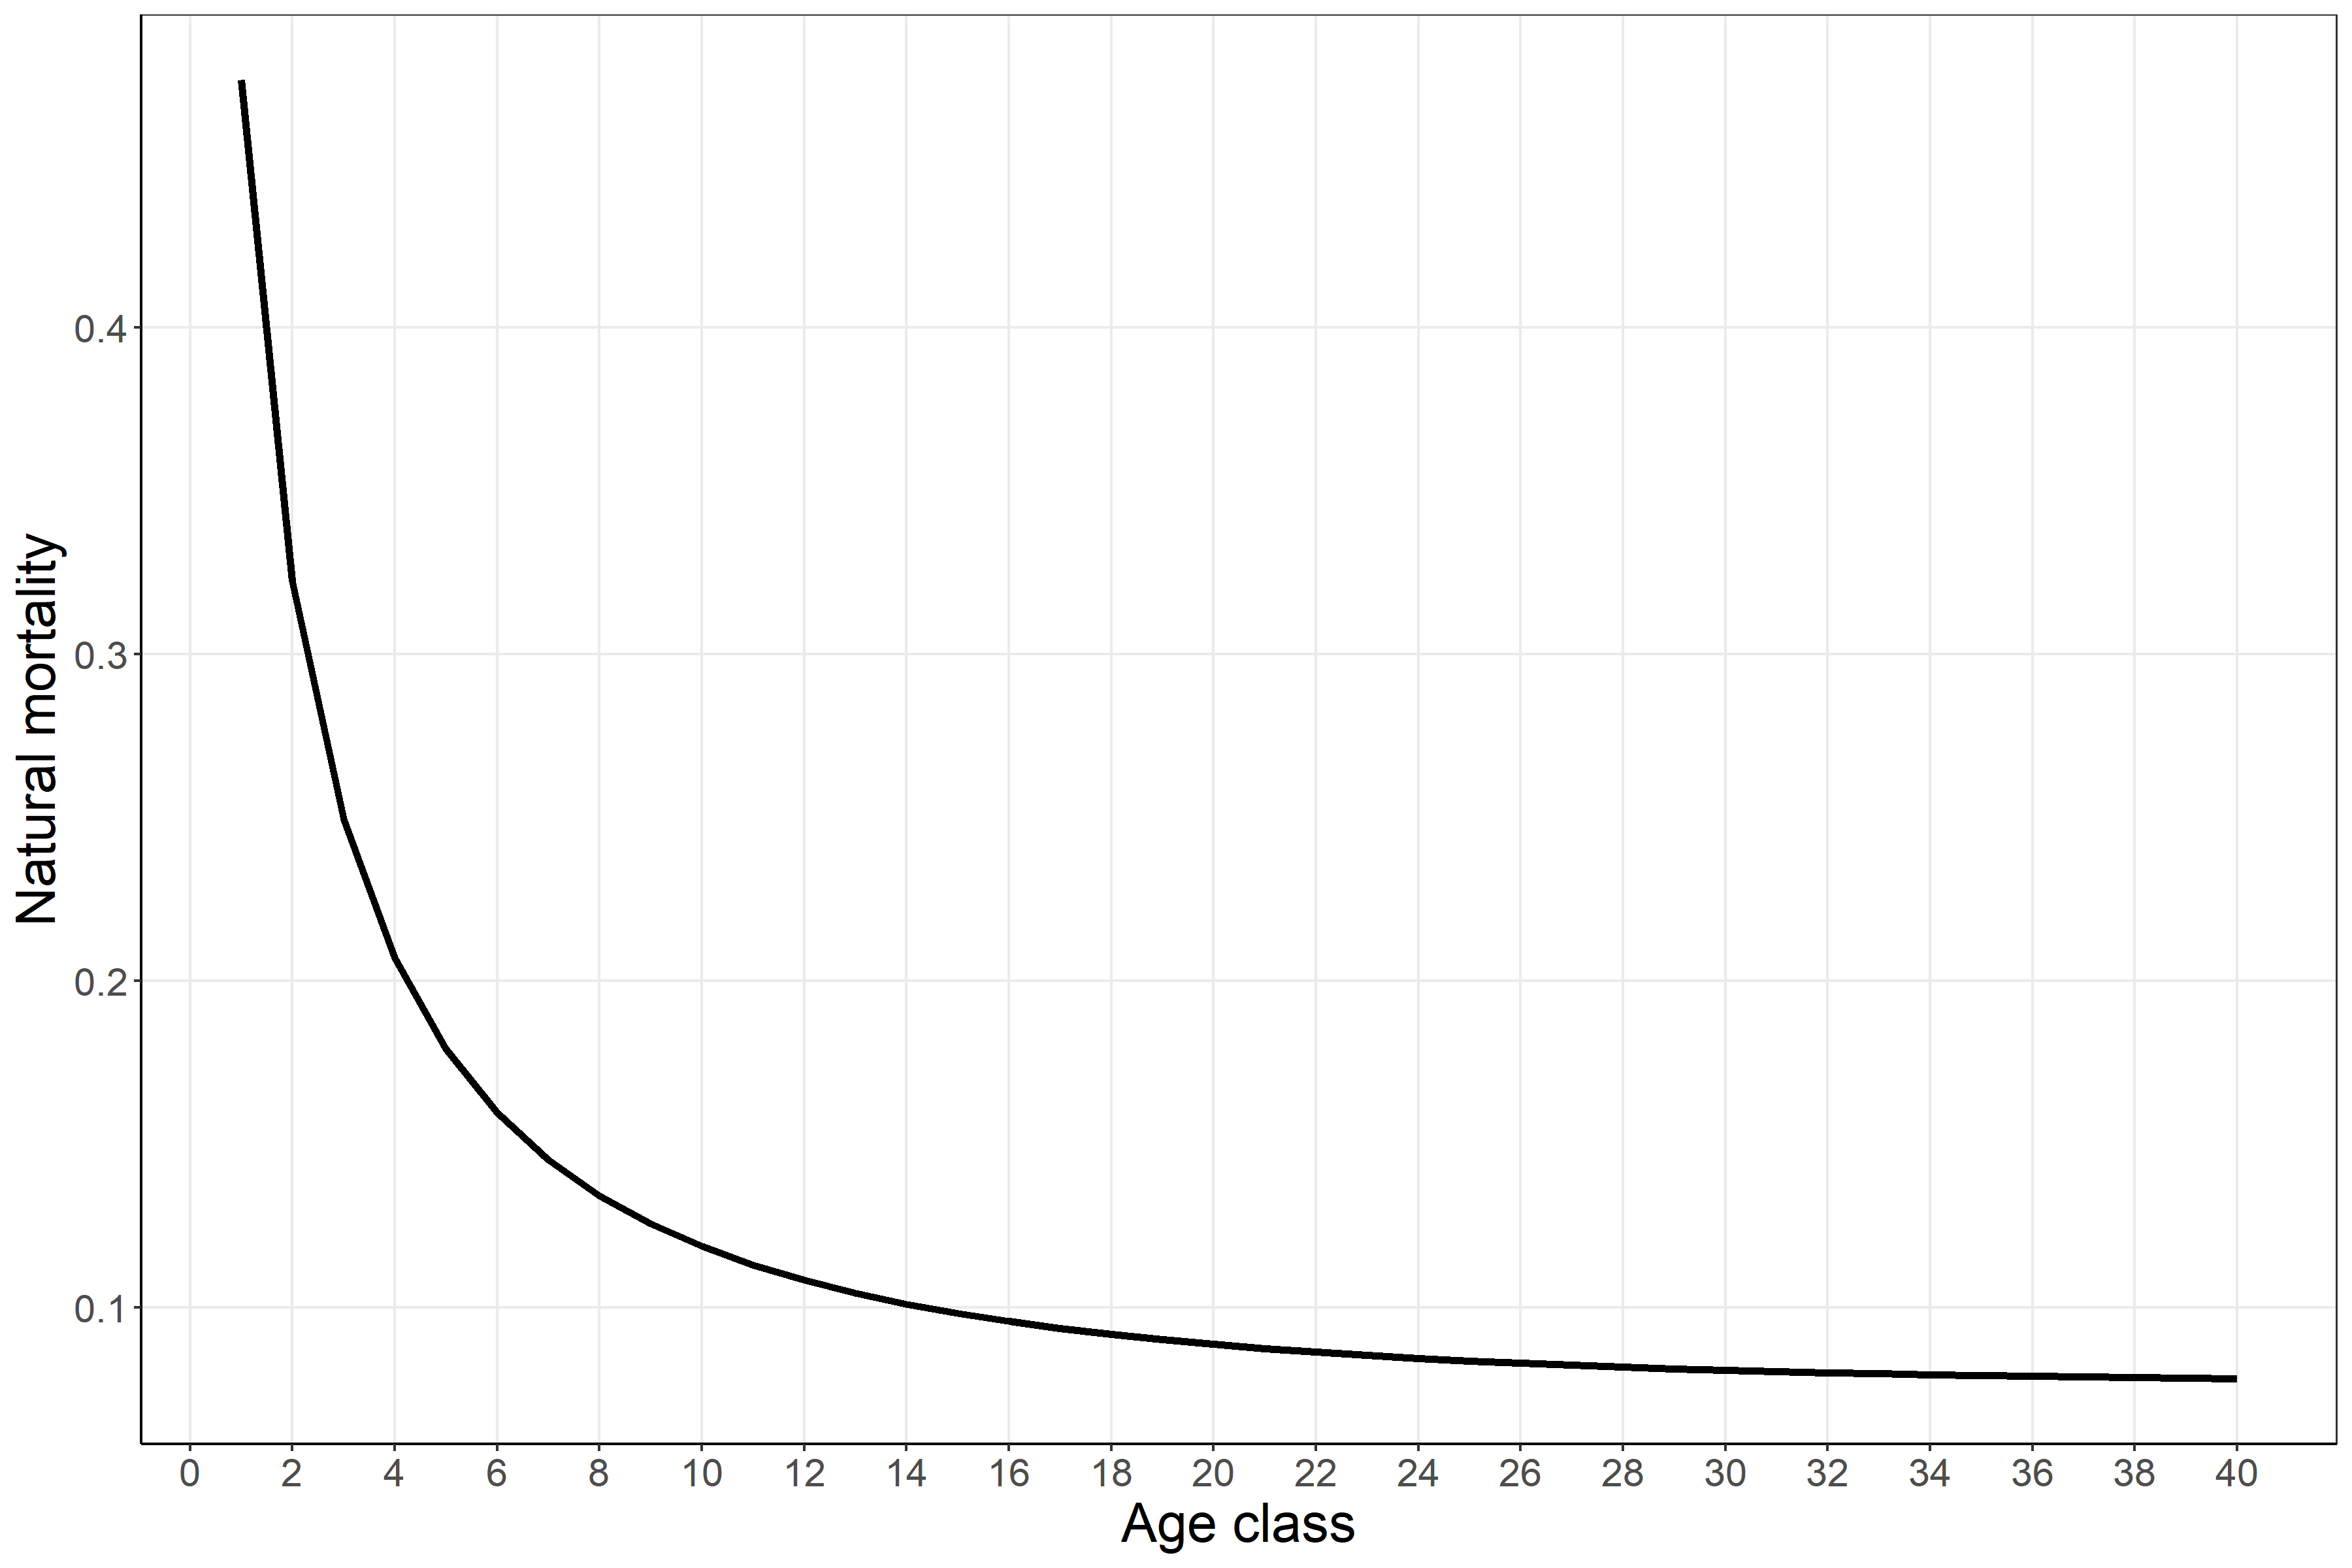
\includegraphics[width=1\linewidth,height=\textheight,keepaspectratio]{figures/natm_at_age.png}

}

\caption{\label{fig-natm-at-age}Lorenzen natural mortality-at-age
(quarters) for the 2026 diagnostic model, based on M at age 40 quarters
of 0.078.}

\end{figure}%

\begin{figure}[H]

\centering{

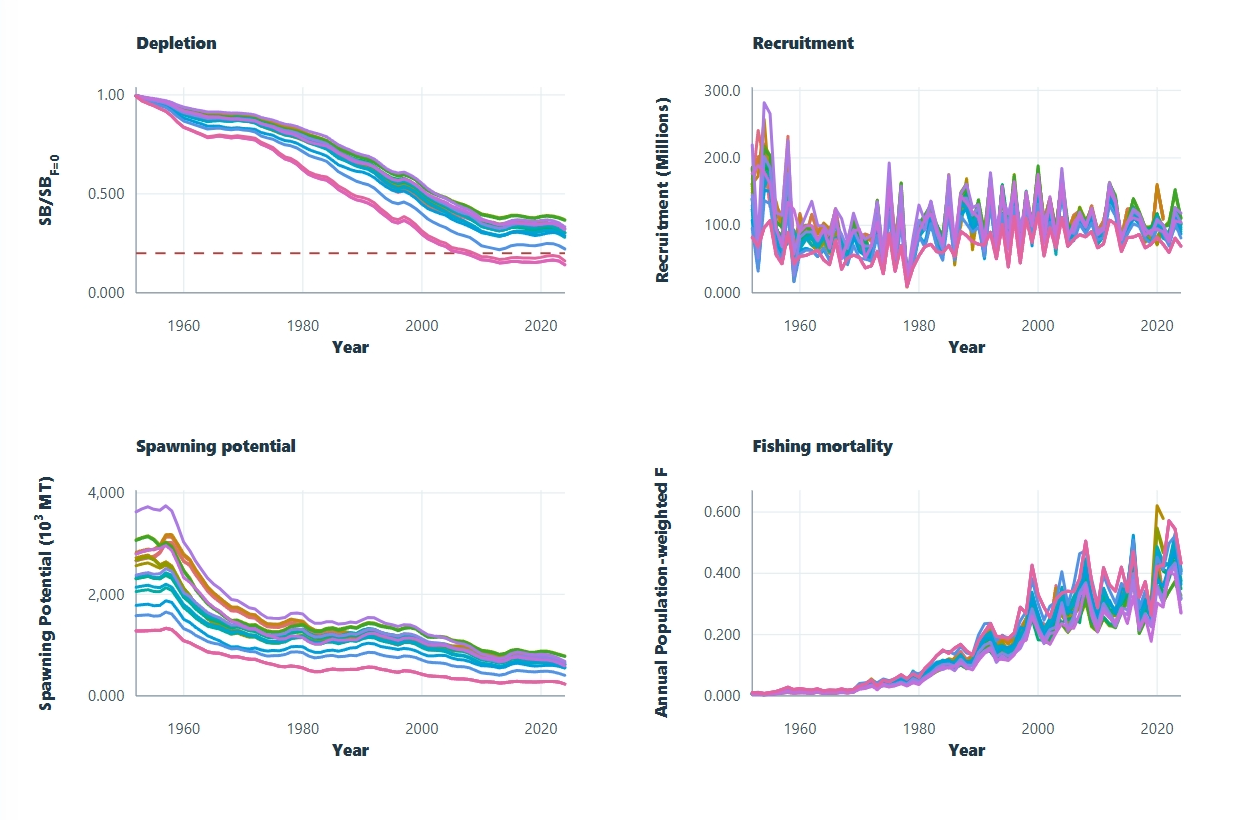
\includegraphics[width=1\linewidth,height=\textheight,keepaspectratio]{figures/stepwise_panel.png}

}

\caption{\label{fig-stepwise-panel}Stepwise model changes for depletion,
recruitment, spawning potential and fishing mortality. The individual
stepwise model changes can be explored in the
\href{https://pacificcommunity.github.io/ofp-sam-bet-2026-stepwise/interactive-model-viewer.html}{interactive
HTML viewer}.}

\end{figure}%

\DIFdelbegin %DIFDELCMD < \begin{figure}[H]
%DIFDELCMD <

%DIFDELCMD < \centering{
%DIFDELCMD <

%DIFDELCMD < 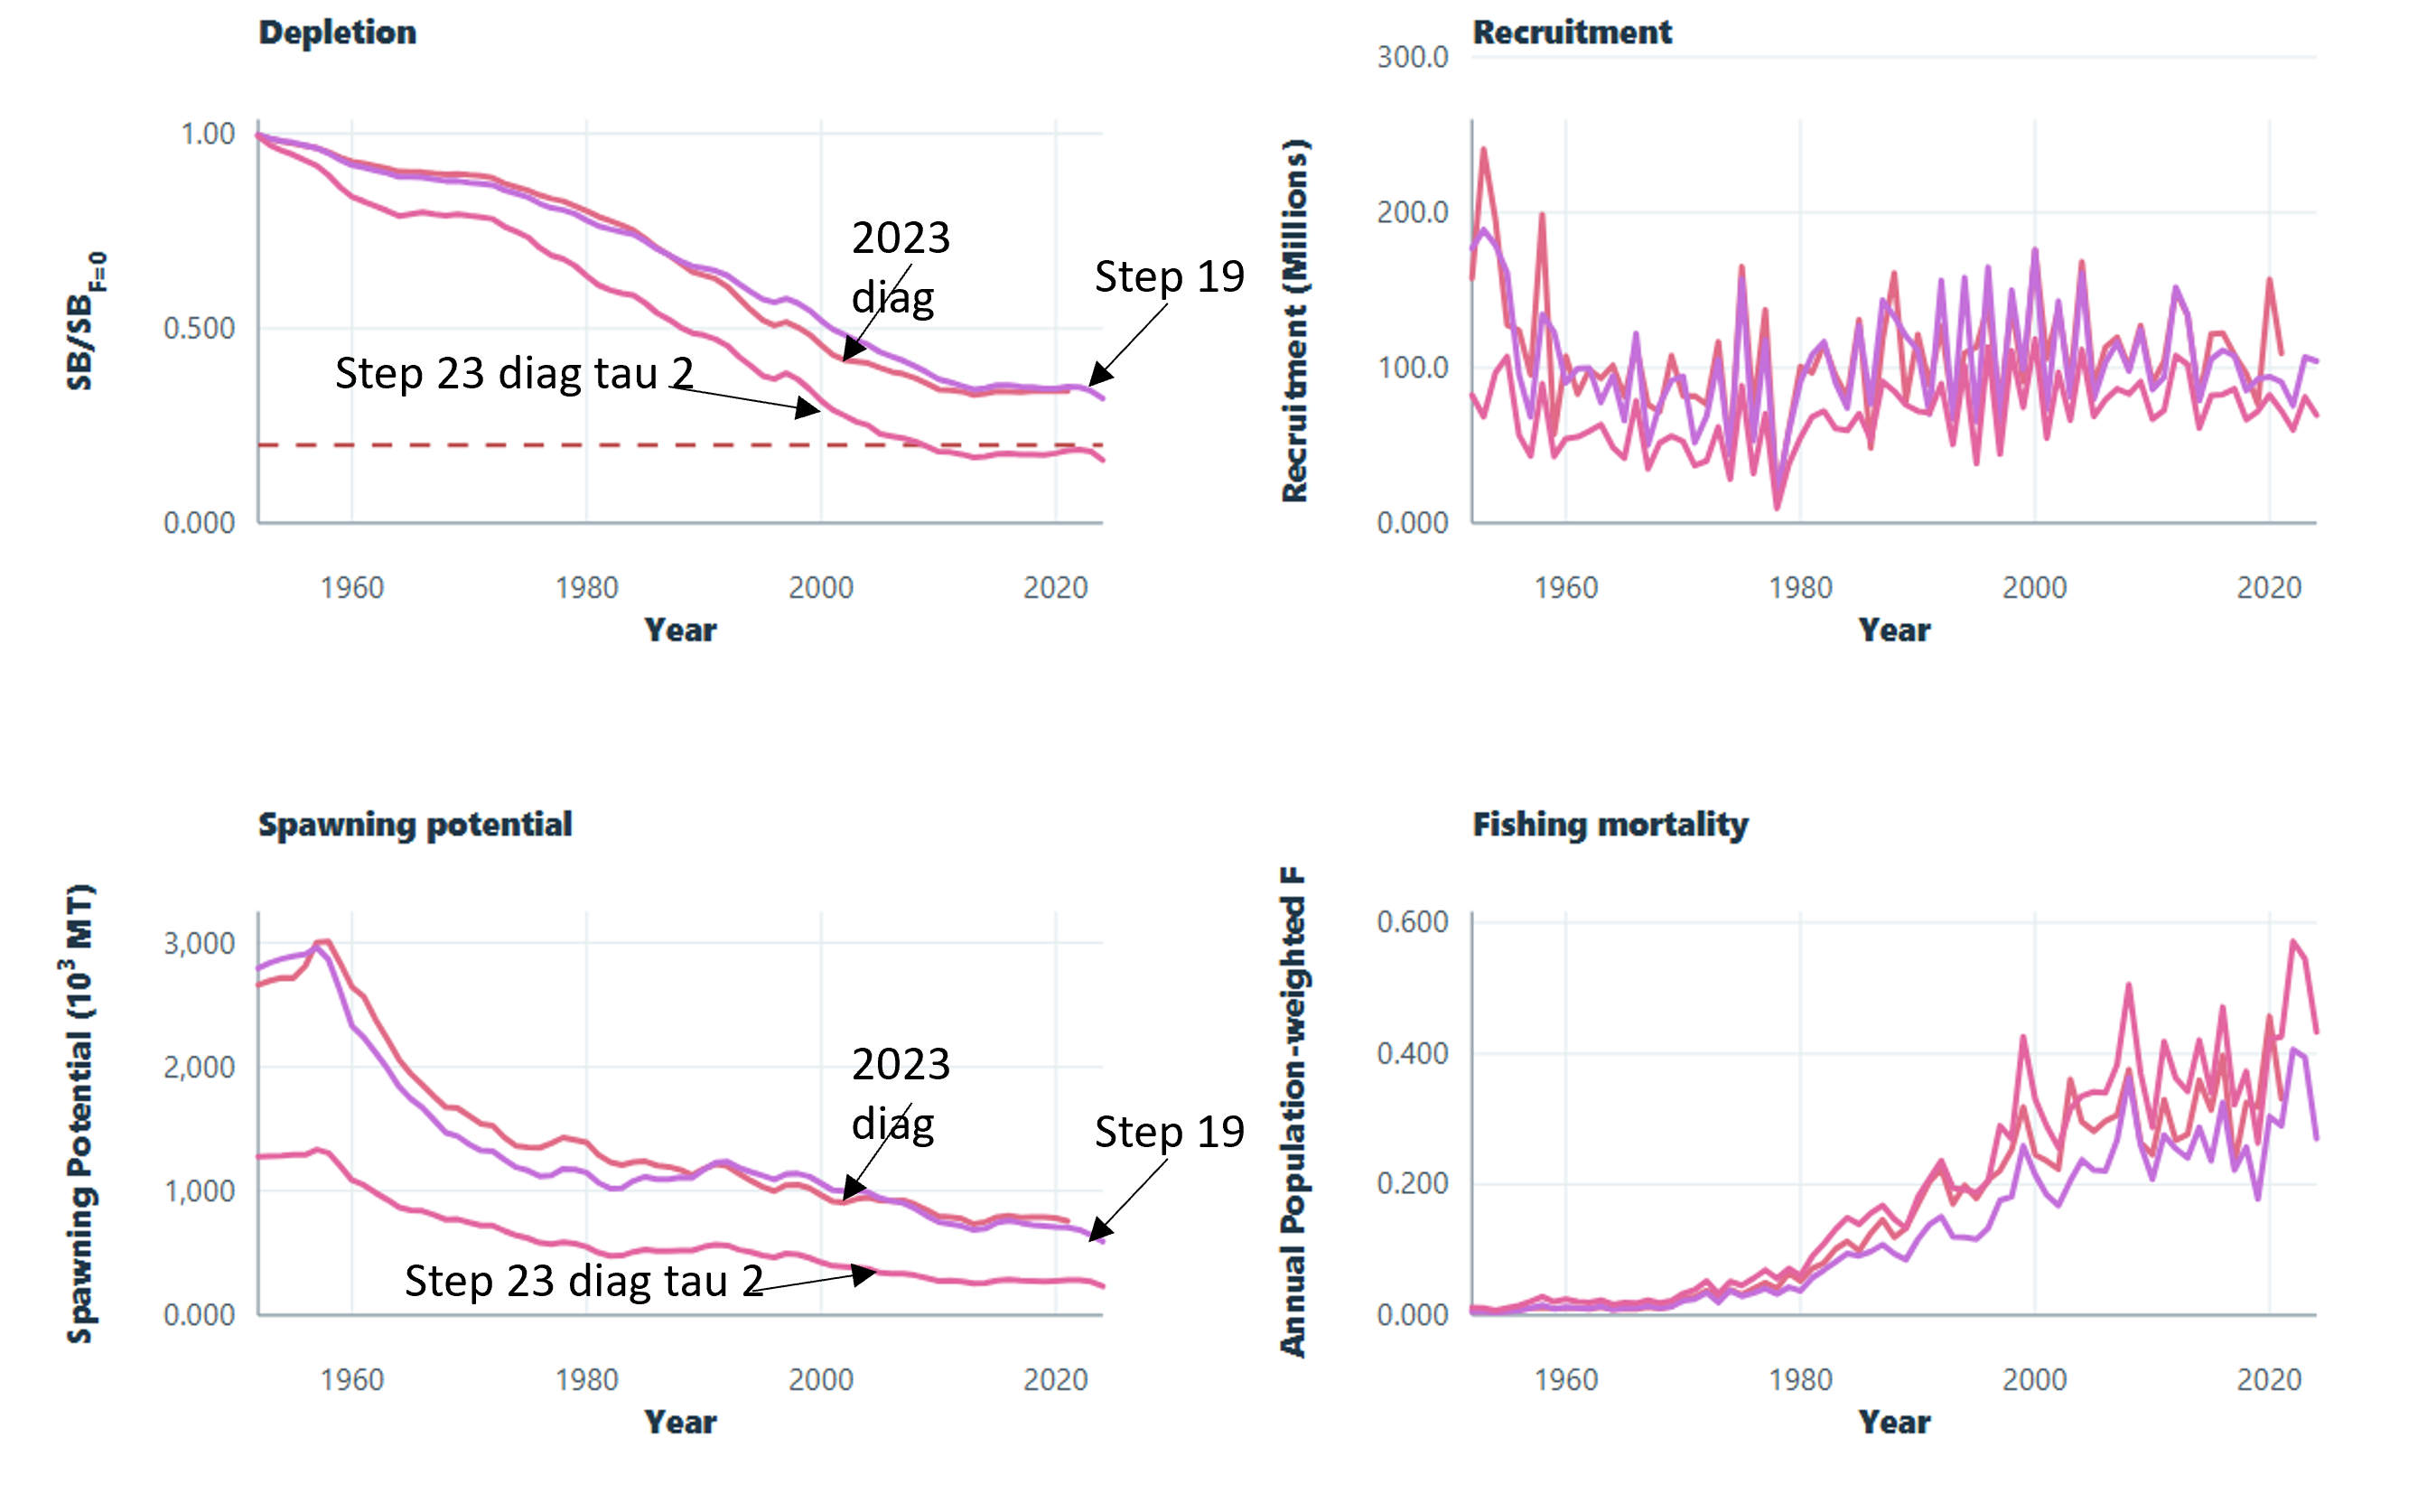
\includegraphics[width=1\linewidth,height=\textheight,keepaspectratio]{figures/stepwise_panel_reduce.png}
%DIFDELCMD <

%DIFDELCMD < }
%DIFDELCMD <

%DIFDELCMD < \caption{\label{fig-stepwise-panel-reduce}Stepwise model changes for
%DIFDELCMD < depletion (\(SB\)/\(SB_{F=0}\)), recruitment, spawning potential and
%DIFDELCMD < fishing mortality, showing the minor difference from the 2023 diagnostic
%DIFDELCMD < model and the model at step 19, compared to the 2026 diagnostic model at
%DIFDELCMD < step 23 when tau (\(\tau\)) has changed from 1 to 2}
%DIFDELCMD <

%DIFDELCMD < \end{figure}%%%
\DIFdelend \DIFaddbegin \begin{figure}[H]

\centering{

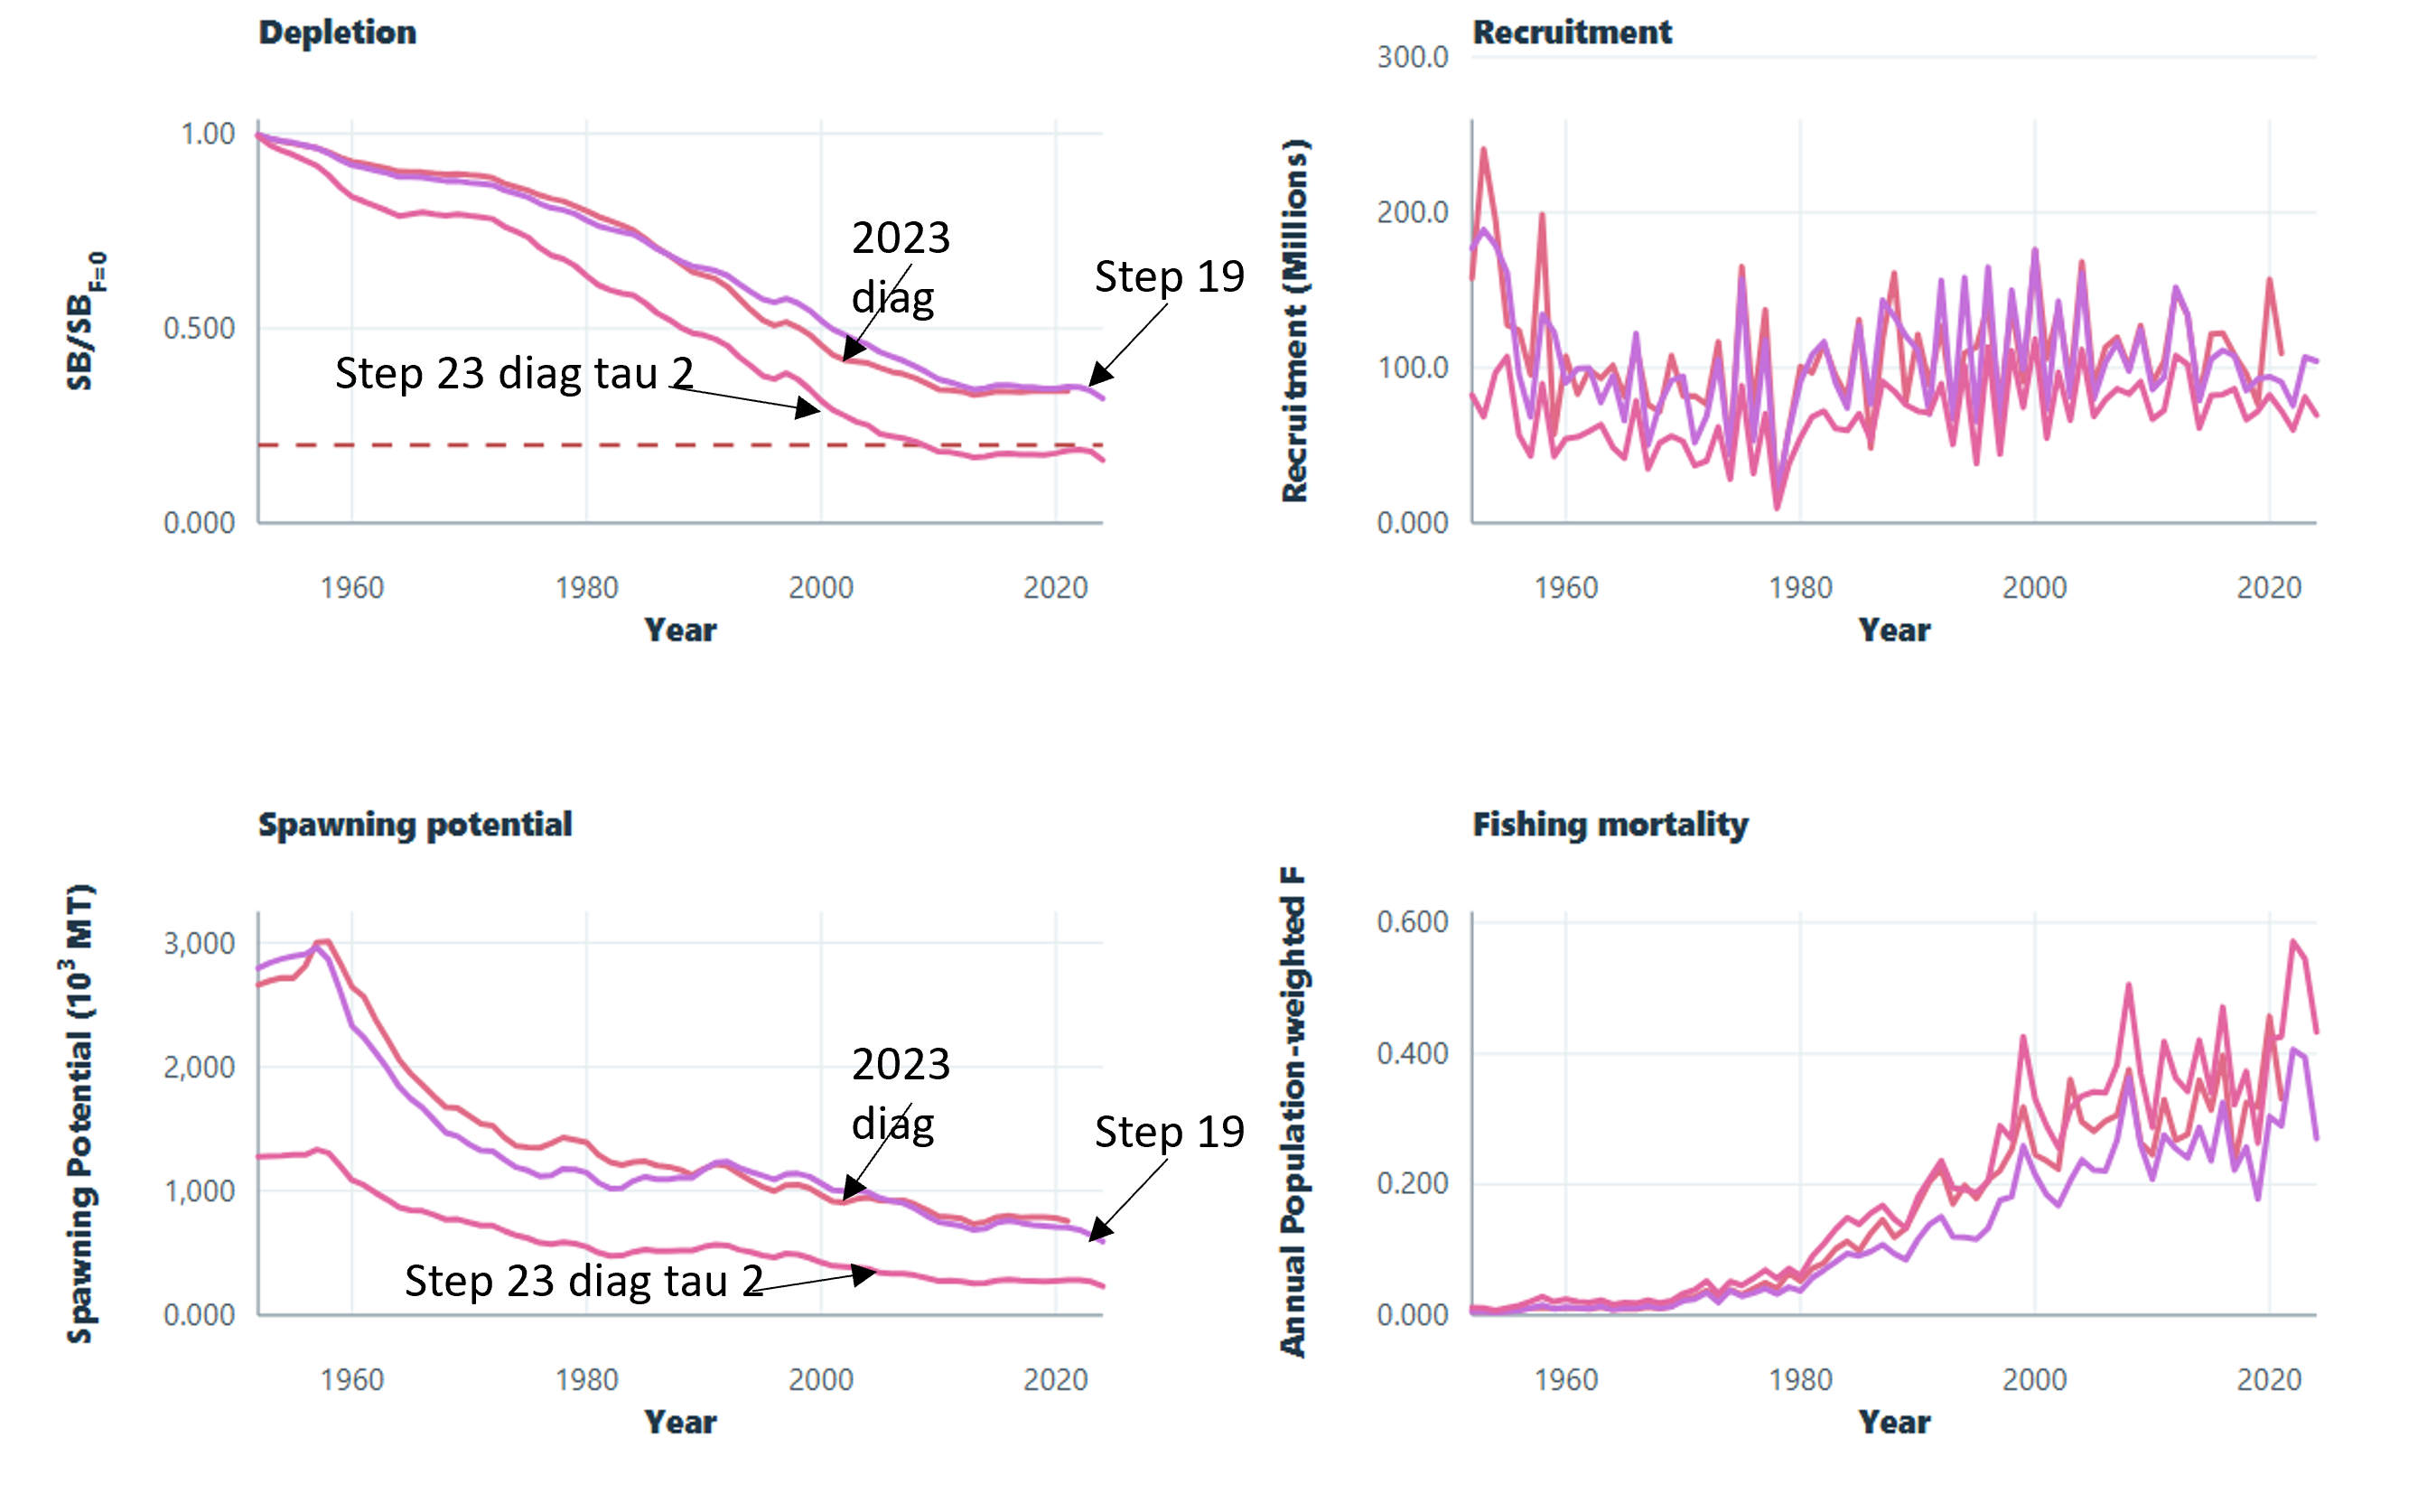
\includegraphics[width=1\linewidth,height=\textheight,keepaspectratio]{figures/stepwise_panel_reduce.png}

}

\caption{\label{fig-stepwise-panel-reduce}Selected stepwise trajectories
for depletion (\(SB\)/\(SB_{F=0}\)), recruitment, spawning potential and
fishing mortality. The figure contrasts the 2023 diagnostic-model refit,
step 19 and the 2026 diagnostic model, highlighting the change after tag
overdispersion \(\tau\) was increased from 1 to 2. Open the
\href{https://pacificcommunity.github.io/ofp-sam-bet-2026-stepwise/interactive-model-viewer.html}{interactive
stepwise viewer}.}

\end{figure}\DIFaddend %

\DIFdelbegin %DIFDELCMD < \begin{figure}[H]
%DIFDELCMD <

%DIFDELCMD < \centering{
%DIFDELCMD <

%DIFDELCMD < 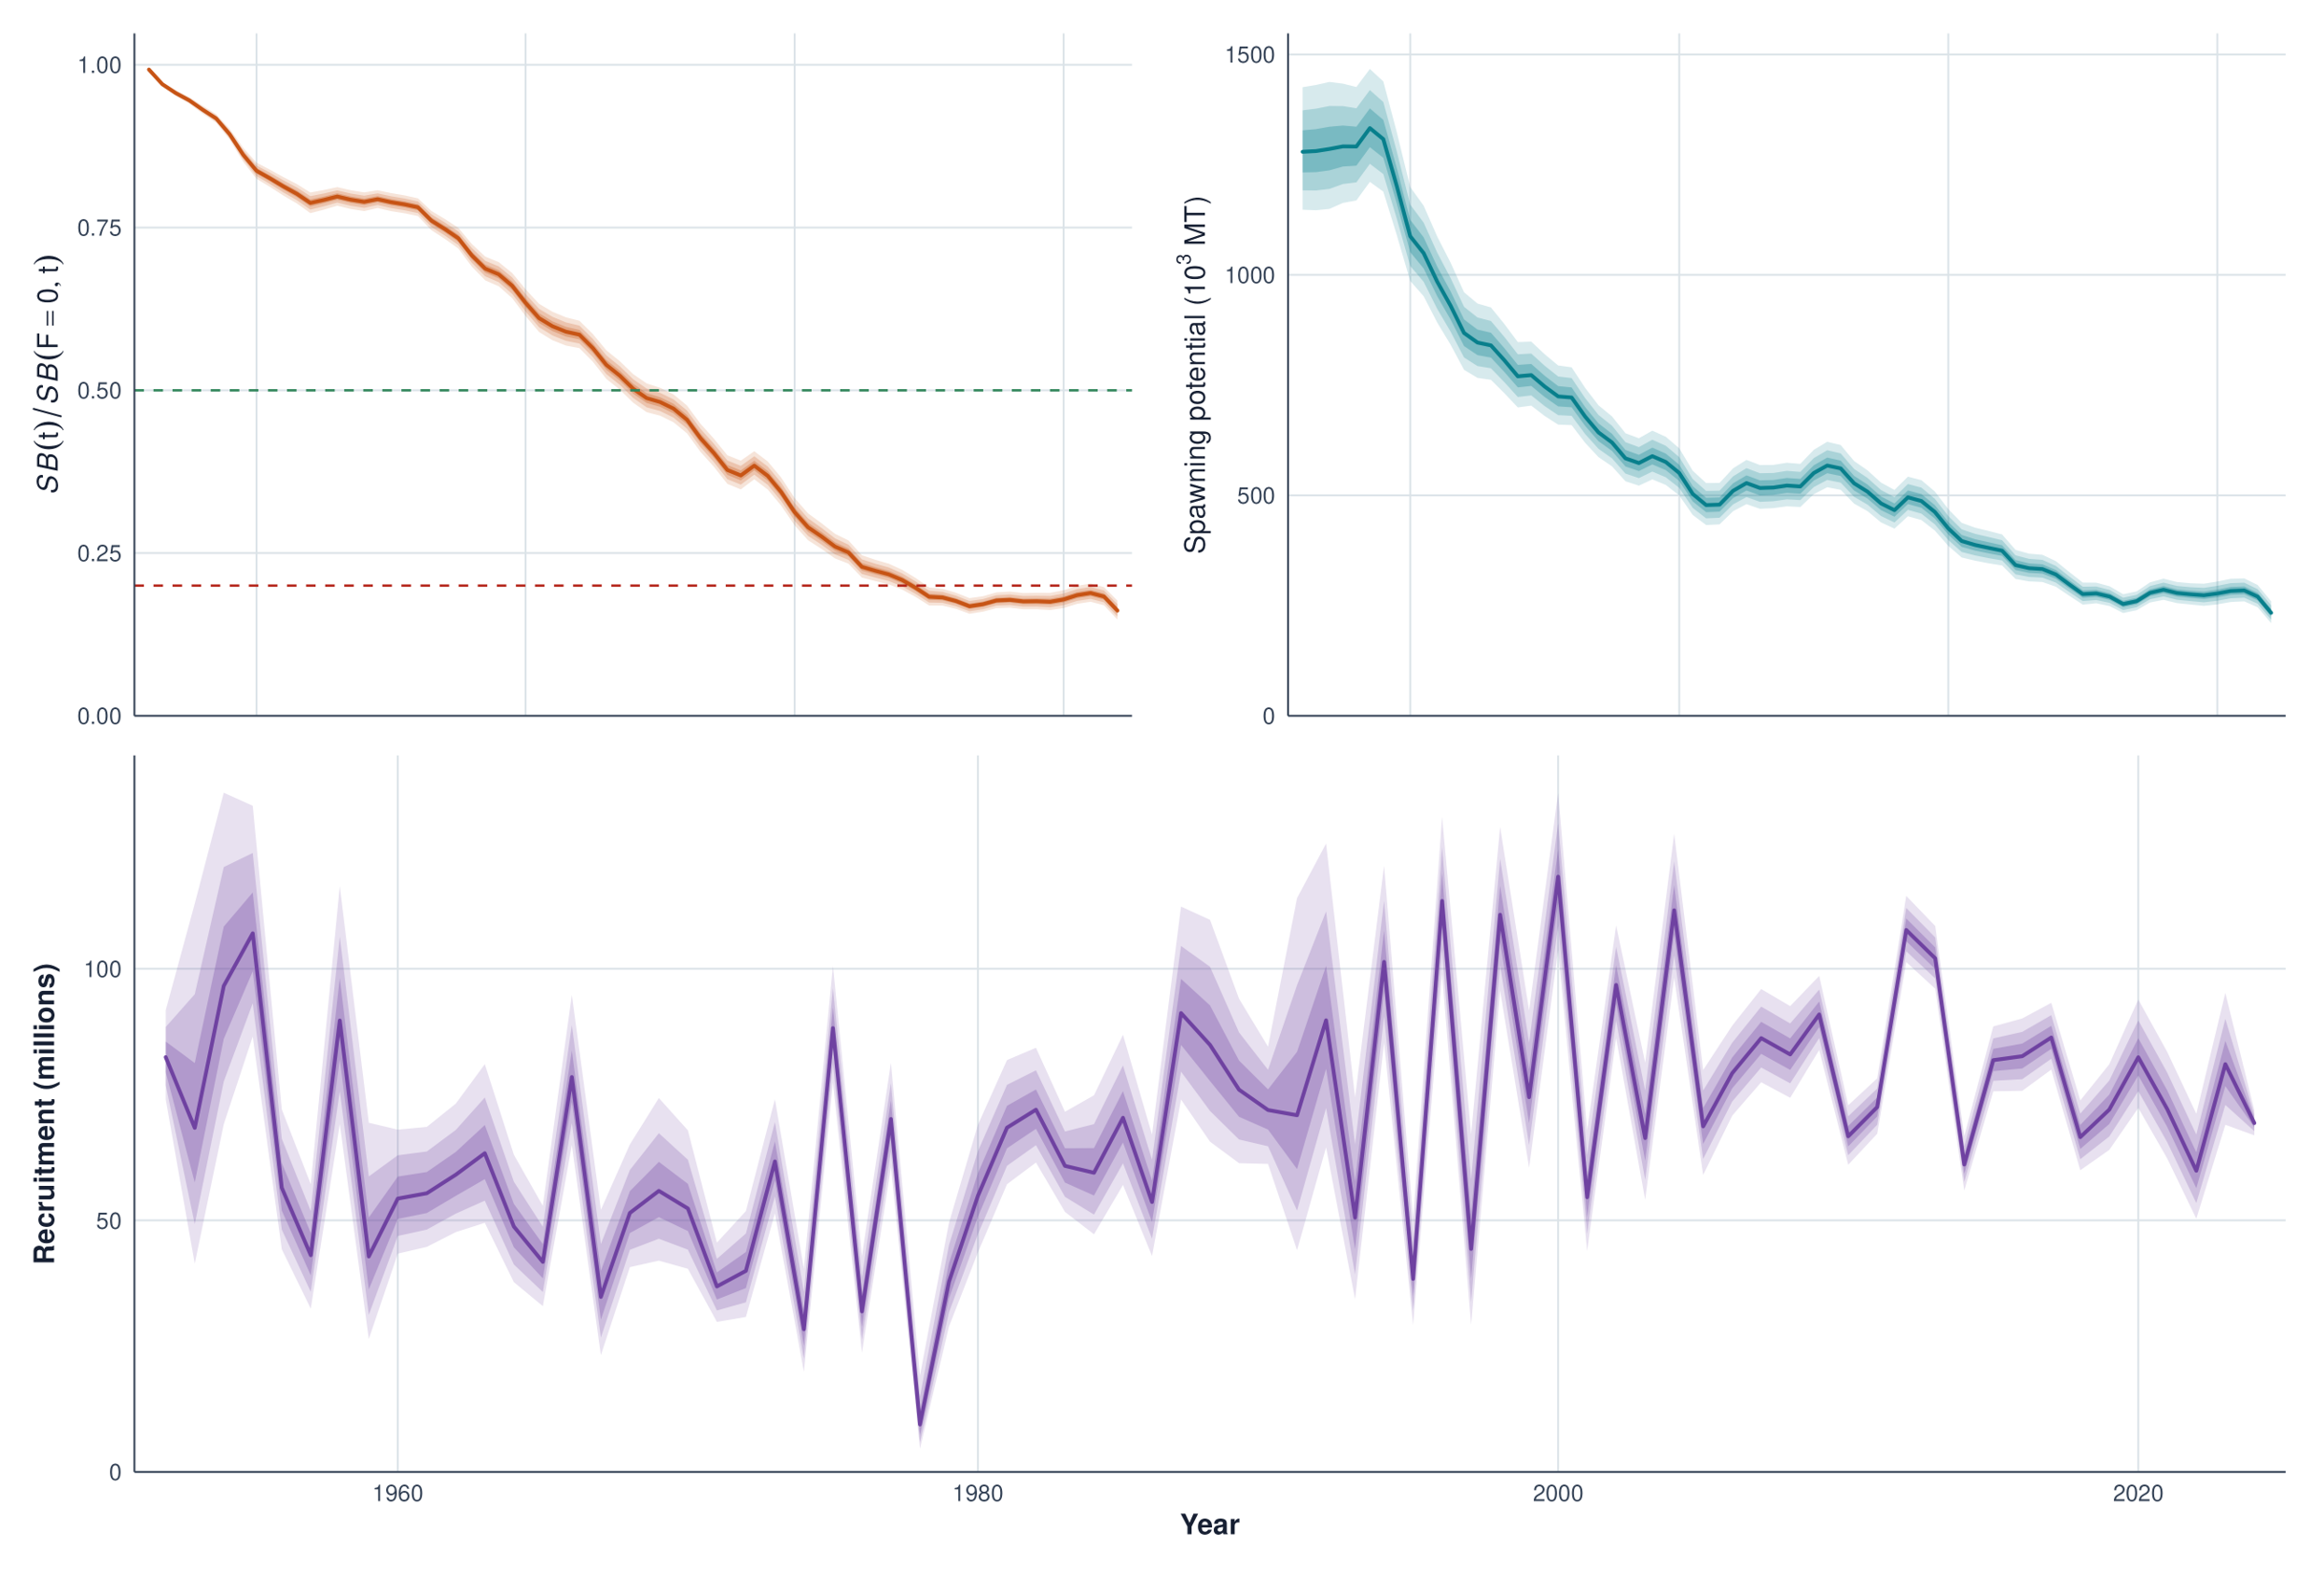
\includegraphics[width=1\linewidth,height=\textheight,keepaspectratio]{figures/diag_time_series.png}
%DIFDELCMD <

%DIFDELCMD < }
%DIFDELCMD <

%DIFDELCMD < \caption{\label{fig-diag-time-series}Population dynamics summary for
%DIFDELCMD < depletion (\(SB\)/\(SB_{F=0}\)), recruitment, spawning potential and
%DIFDELCMD < fishing mortality, for the diagnostic model}
%DIFDELCMD <

%DIFDELCMD < \end{figure}%%%
\DIFdelend \DIFaddbegin \begin{figure}[H]

\centering{

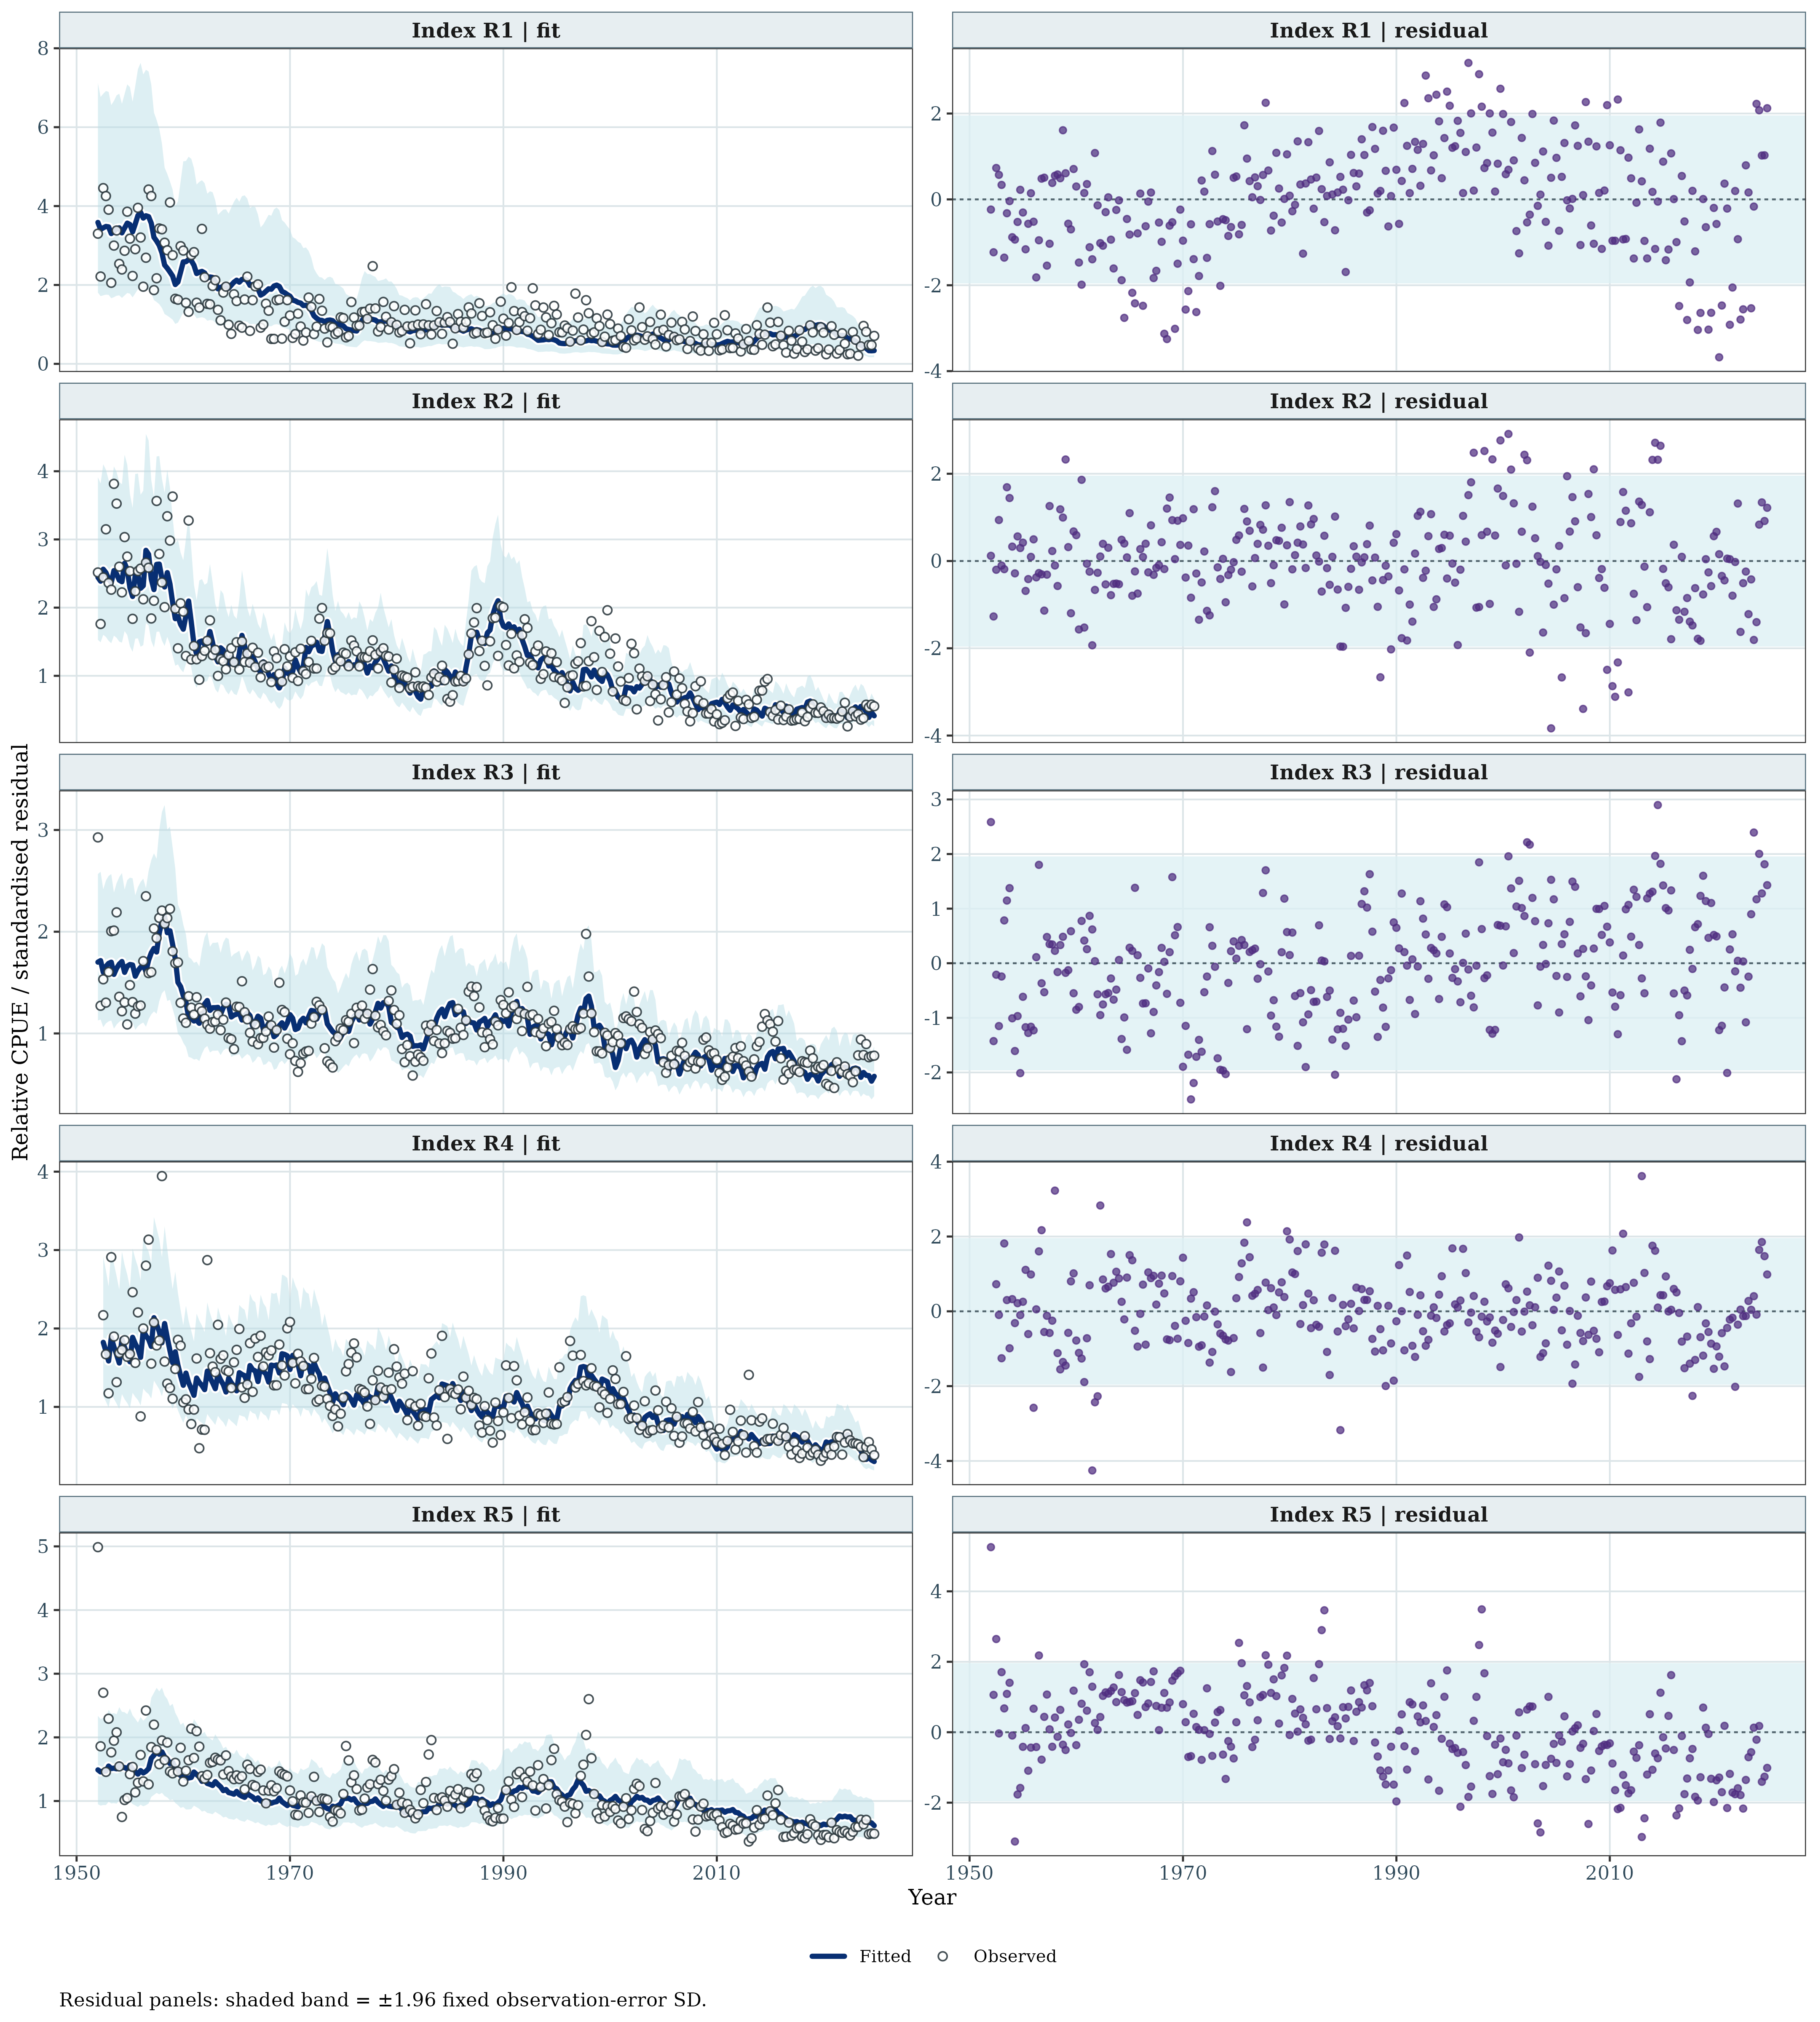
\includegraphics[width=1\linewidth,height=\textheight,keepaspectratio]{figures_new/cpue-fit-residuals.png}

}

\caption{\label{fig-cpue-fit-residuals}\label{fig-cpue-fit-1-5}\label{fig-cpue-resids-1-5}Observed and fitted relative CPUE
(left panels) with standardised log-scale residuals (right panels) for
the five regional index fisheries. Fit shading gives the central 95\%
observation interval implied by the fixed regional log-scale error
values; it is not parameter-estimation uncertainty. Residual shading
marks the corresponding \(\pm 1.96\) observation-error SD range. Open
the
\href{https://pacificcommunity.github.io/ofp-sam-bet-2026-diagnostic/bet-2026-diagnostic-report.html}{interactive
diagnostic report}.}

\end{figure}\DIFaddend %

\DIFdelbegin %DIFDELCMD < \begin{figure}[H]
%DIFDELCMD <

%DIFDELCMD < \centering{
%DIFDELCMD <

%DIFDELCMD < 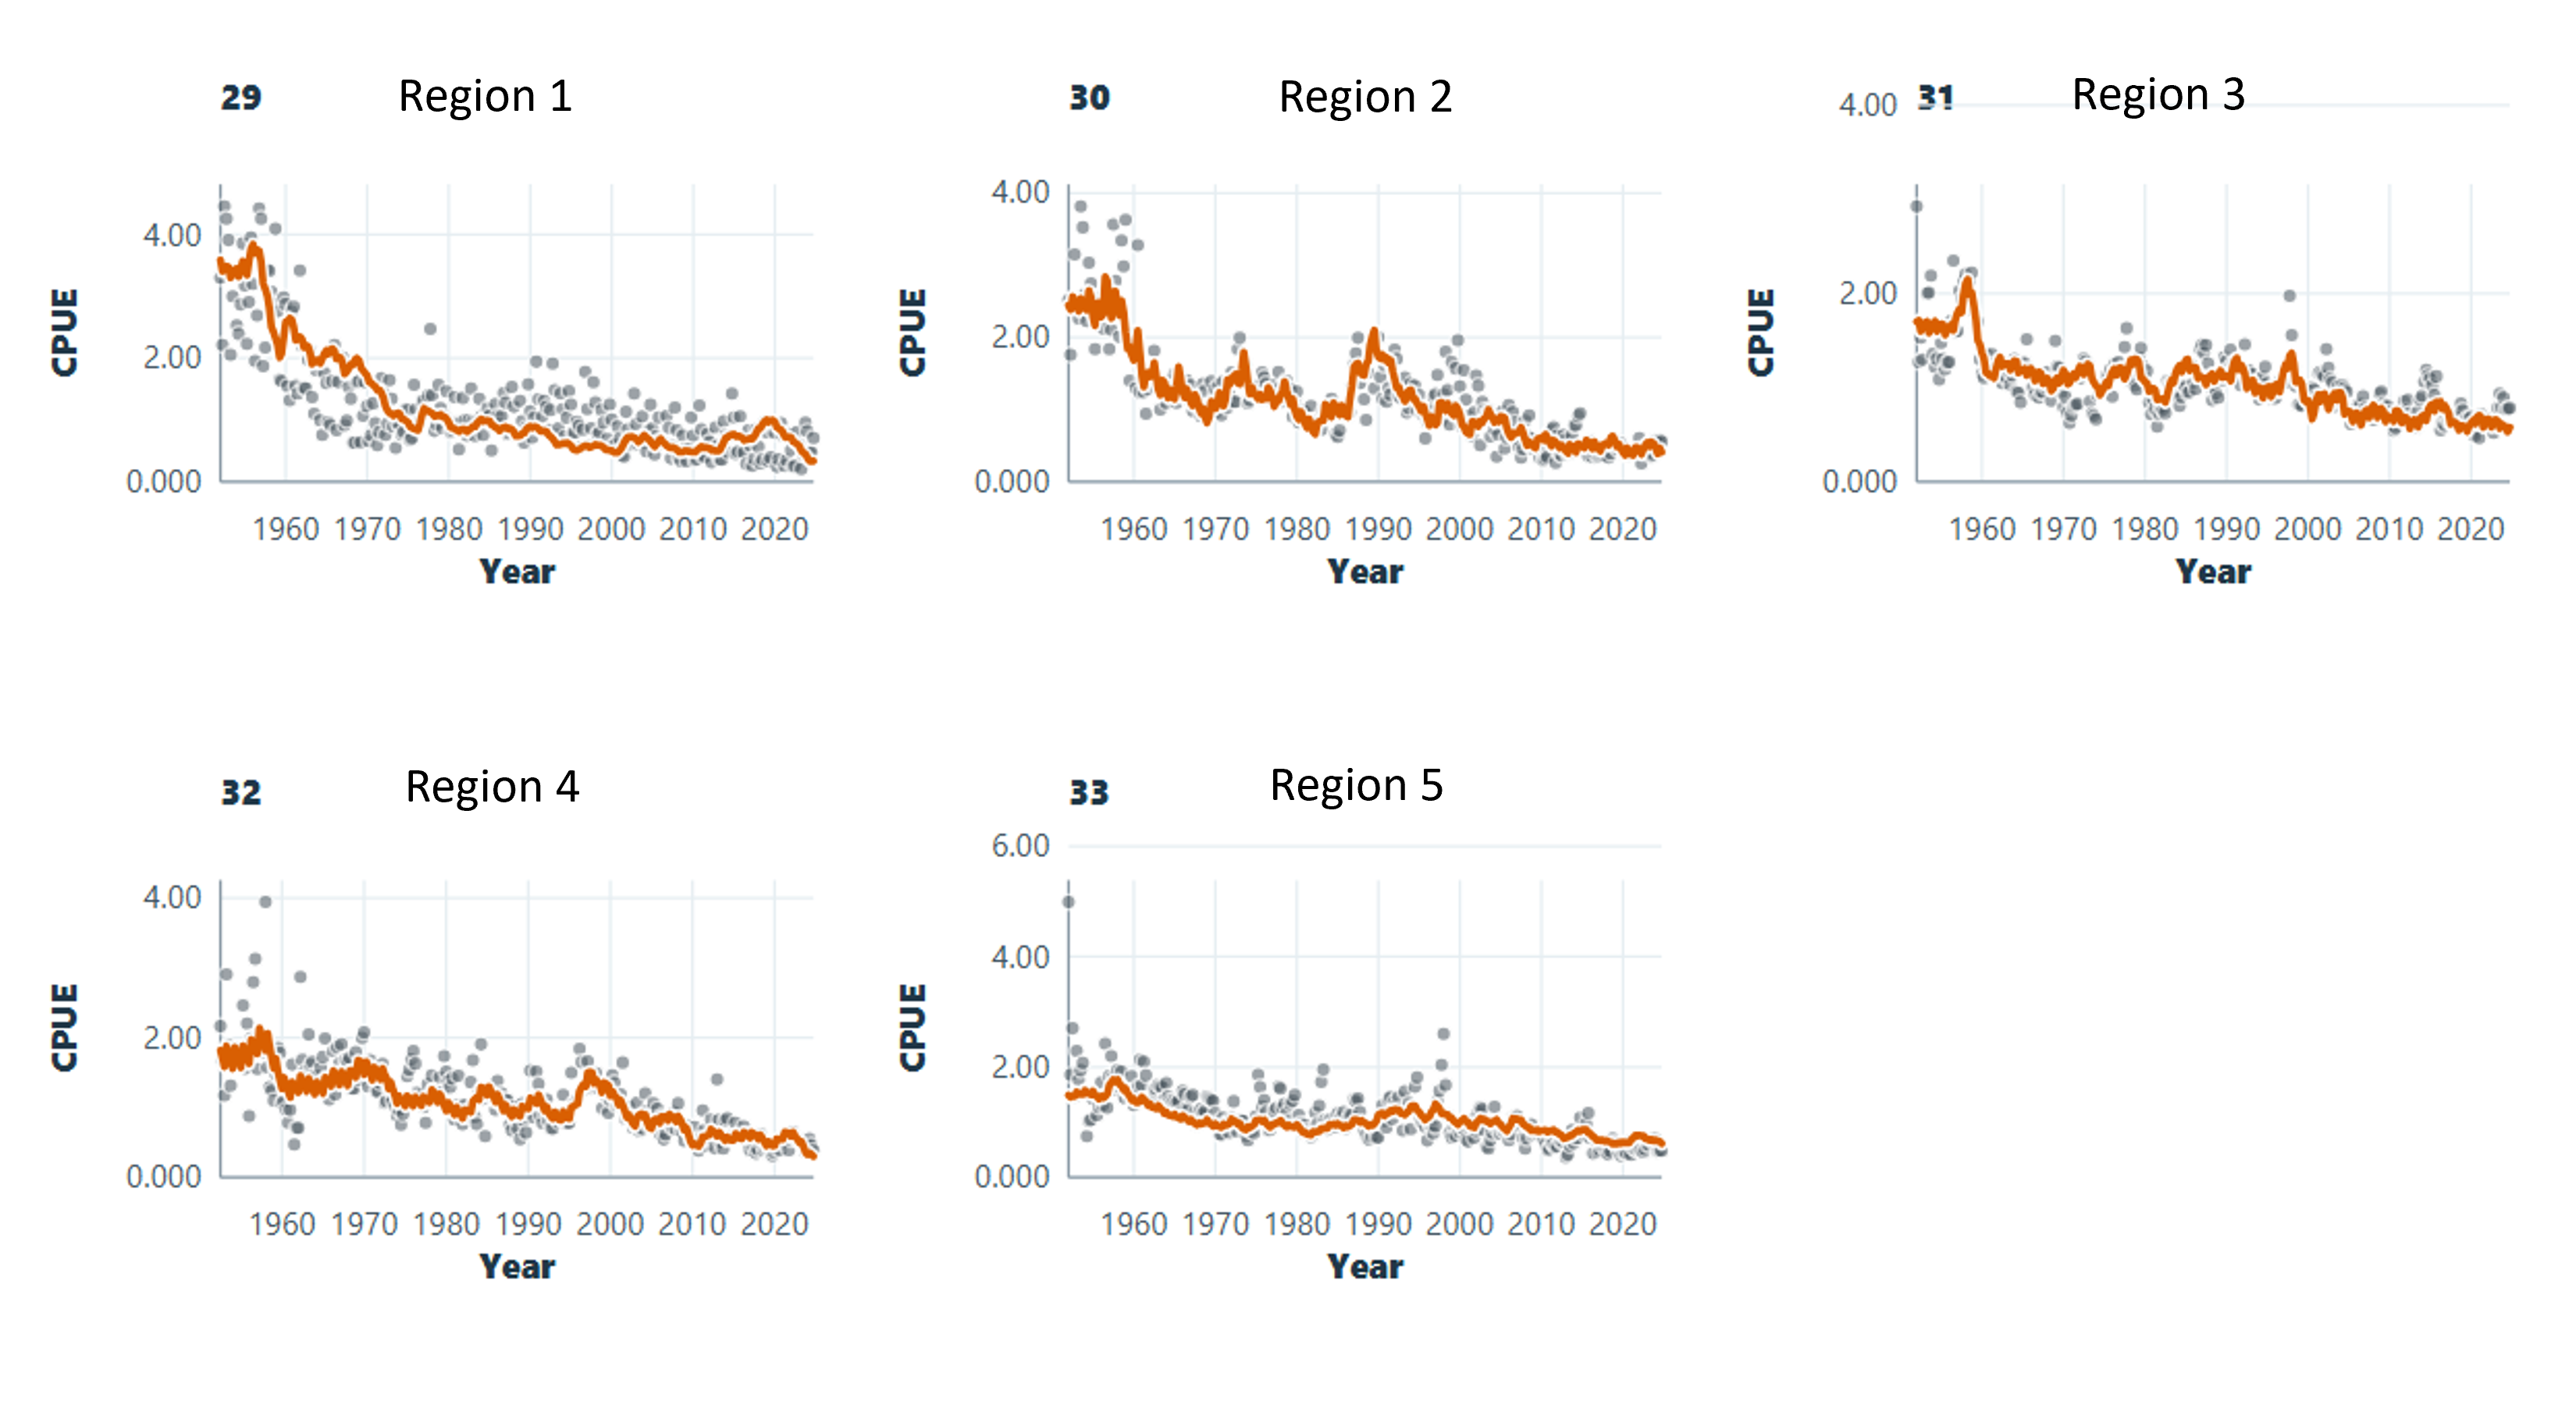
\includegraphics[width=1\linewidth,height=\textheight,keepaspectratio]{figures/cpue_fit_1_5.png}
%DIFDELCMD <

%DIFDELCMD < }
%DIFDELCMD <

%DIFDELCMD < \caption{\label{fig-cpue-fit-1-5}Fits (orange line) to the standardised
%DIFDELCMD < CPUE (gray dots) for the longline index fisheries in region 1-5.}
%DIFDELCMD <

%DIFDELCMD < \end{figure}%%%
\DIFdelend \DIFaddbegin \begin{figure}[H]

\centering{

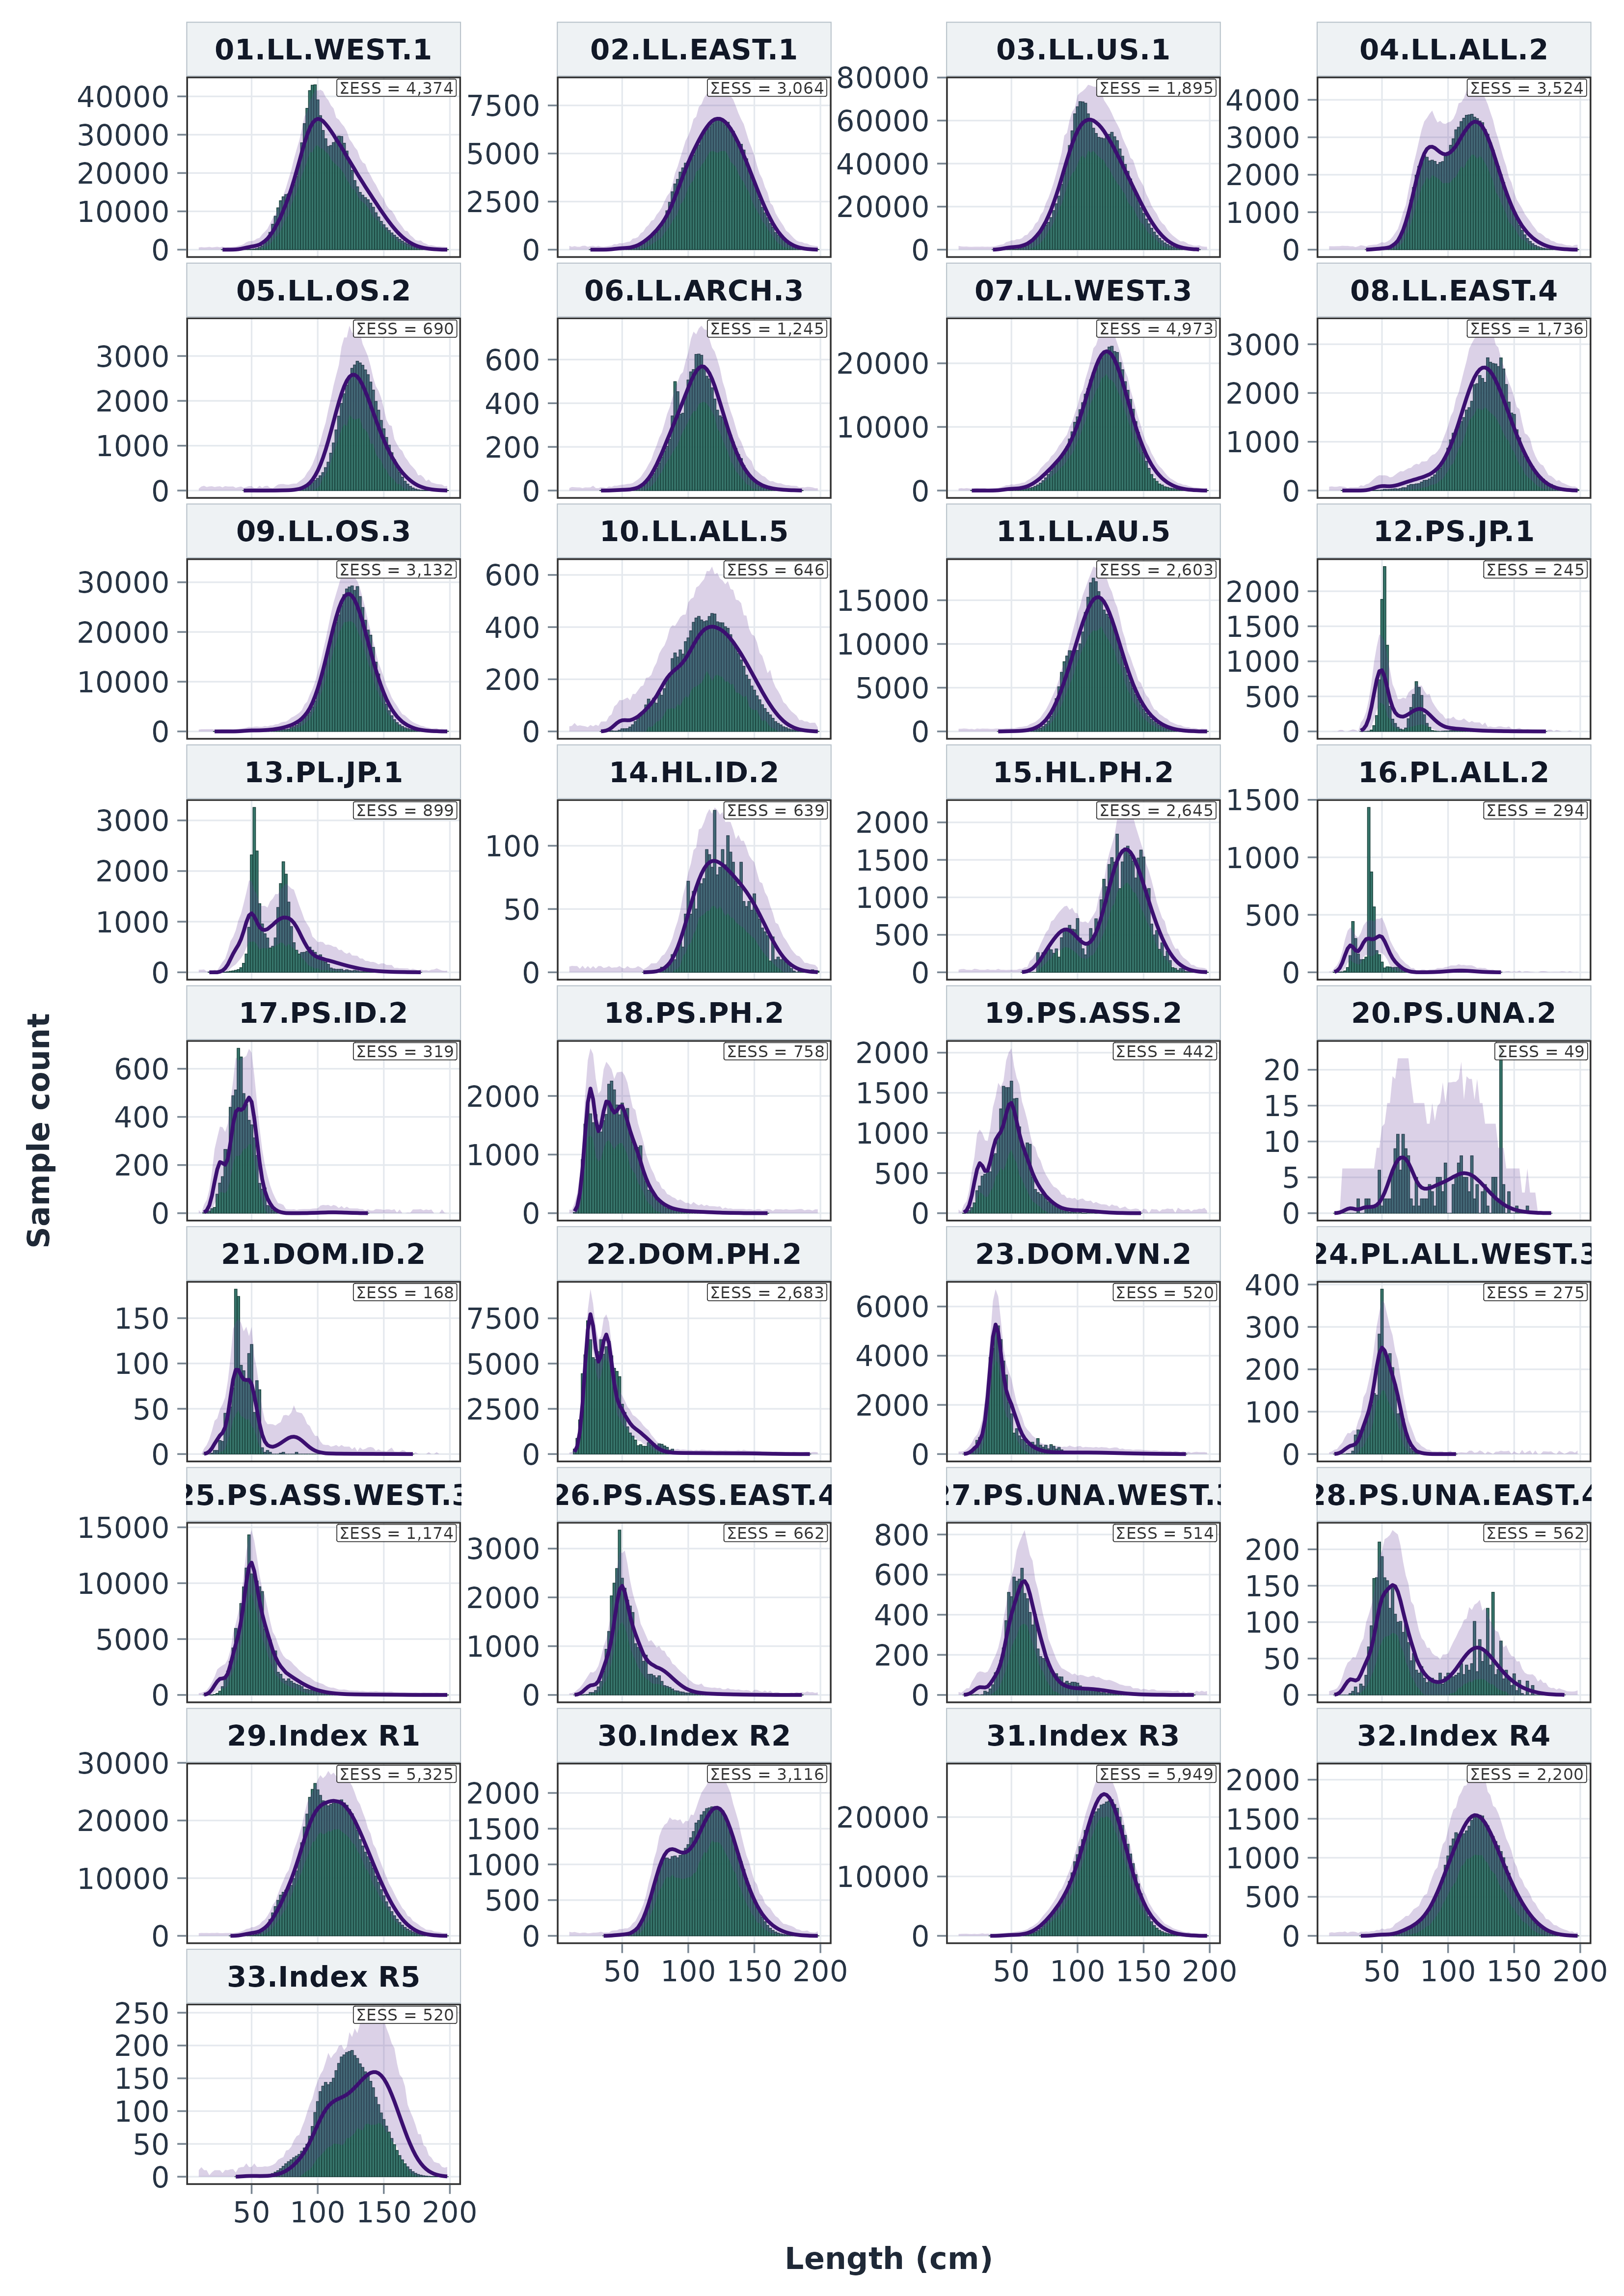
\includegraphics[width=1\linewidth,height=\textheight,keepaspectratio]{figures_new/length-frequency-fit-by-fishery.png}

}

\caption{\label{fig-length-fit-by-fishery}\label{fig-length-fit-aggregated-ll}\label{fig-length-fit-aggregated-dompl}\label{fig-length-fit-aggregated-ps}Observed (bars) and fitted
(purple lines) length-frequency sample counts by fishery, pooled over
years. Shading is the 95\% pointwise conditional predictive interval for
repeated observations under the fitted Dirichlet--multinomial model;
parameter uncertainty is not included. The top-right \(\Sigma\)ESS is
the sum of model-implied incident effective sample sizes in each
fishery. Open the
\href{https://pacificcommunity.github.io/ofp-sam-bet-2026-diagnostic/bet-2026-diagnostic-report.html}{interactive
diagnostic report} for fishery- and year-level selections.}

\end{figure}\DIFaddend %

\DIFdelbegin %DIFDELCMD < \begin{figure}[H]
%DIFDELCMD <

%DIFDELCMD < \centering{
%DIFDELCMD <

%DIFDELCMD < 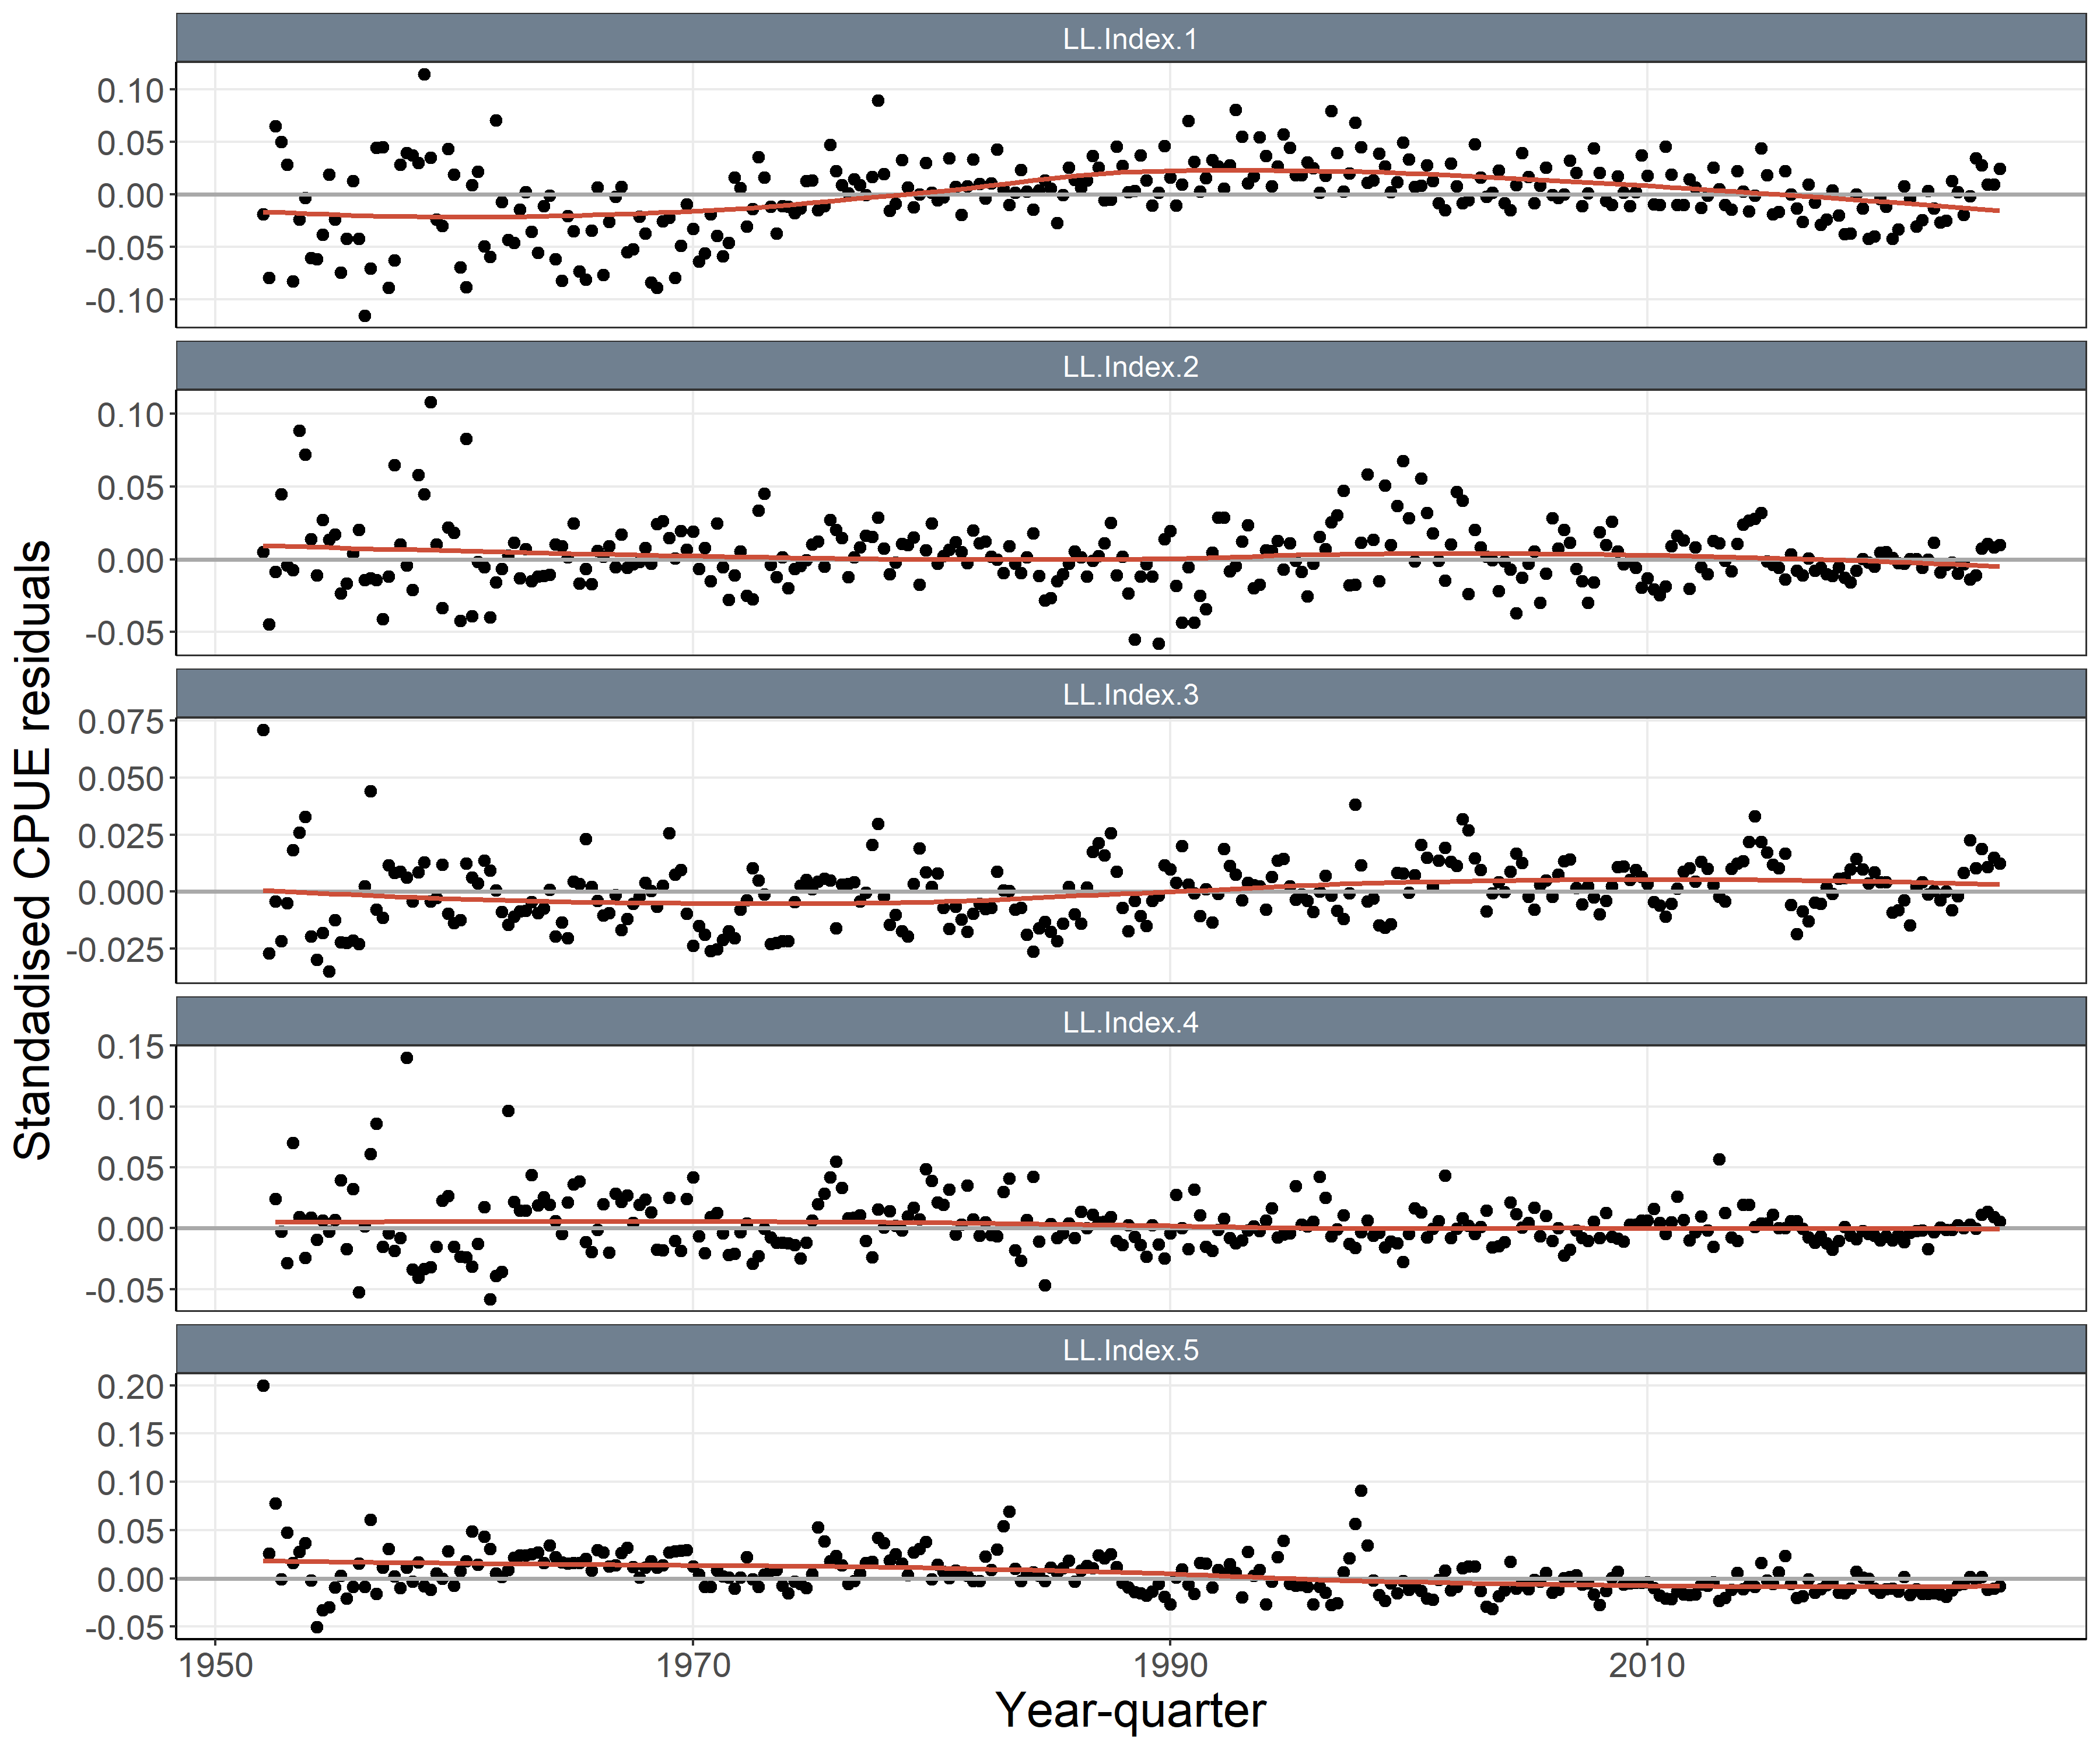
\includegraphics[width=1\linewidth,height=\textheight,keepaspectratio]{figures/cpue_resids_1_5.png}
%DIFDELCMD <

%DIFDELCMD < }
%DIFDELCMD <

%DIFDELCMD < \caption{\label{fig-cpue-resids-1-5}Residuals for the standardised CPUE
%DIFDELCMD < for the longline index fisheries in region 1-5.}
%DIFDELCMD <

%DIFDELCMD < \end{figure}%%%
\DIFdelend \DIFaddbegin \begin{figure}[H]

\centering{

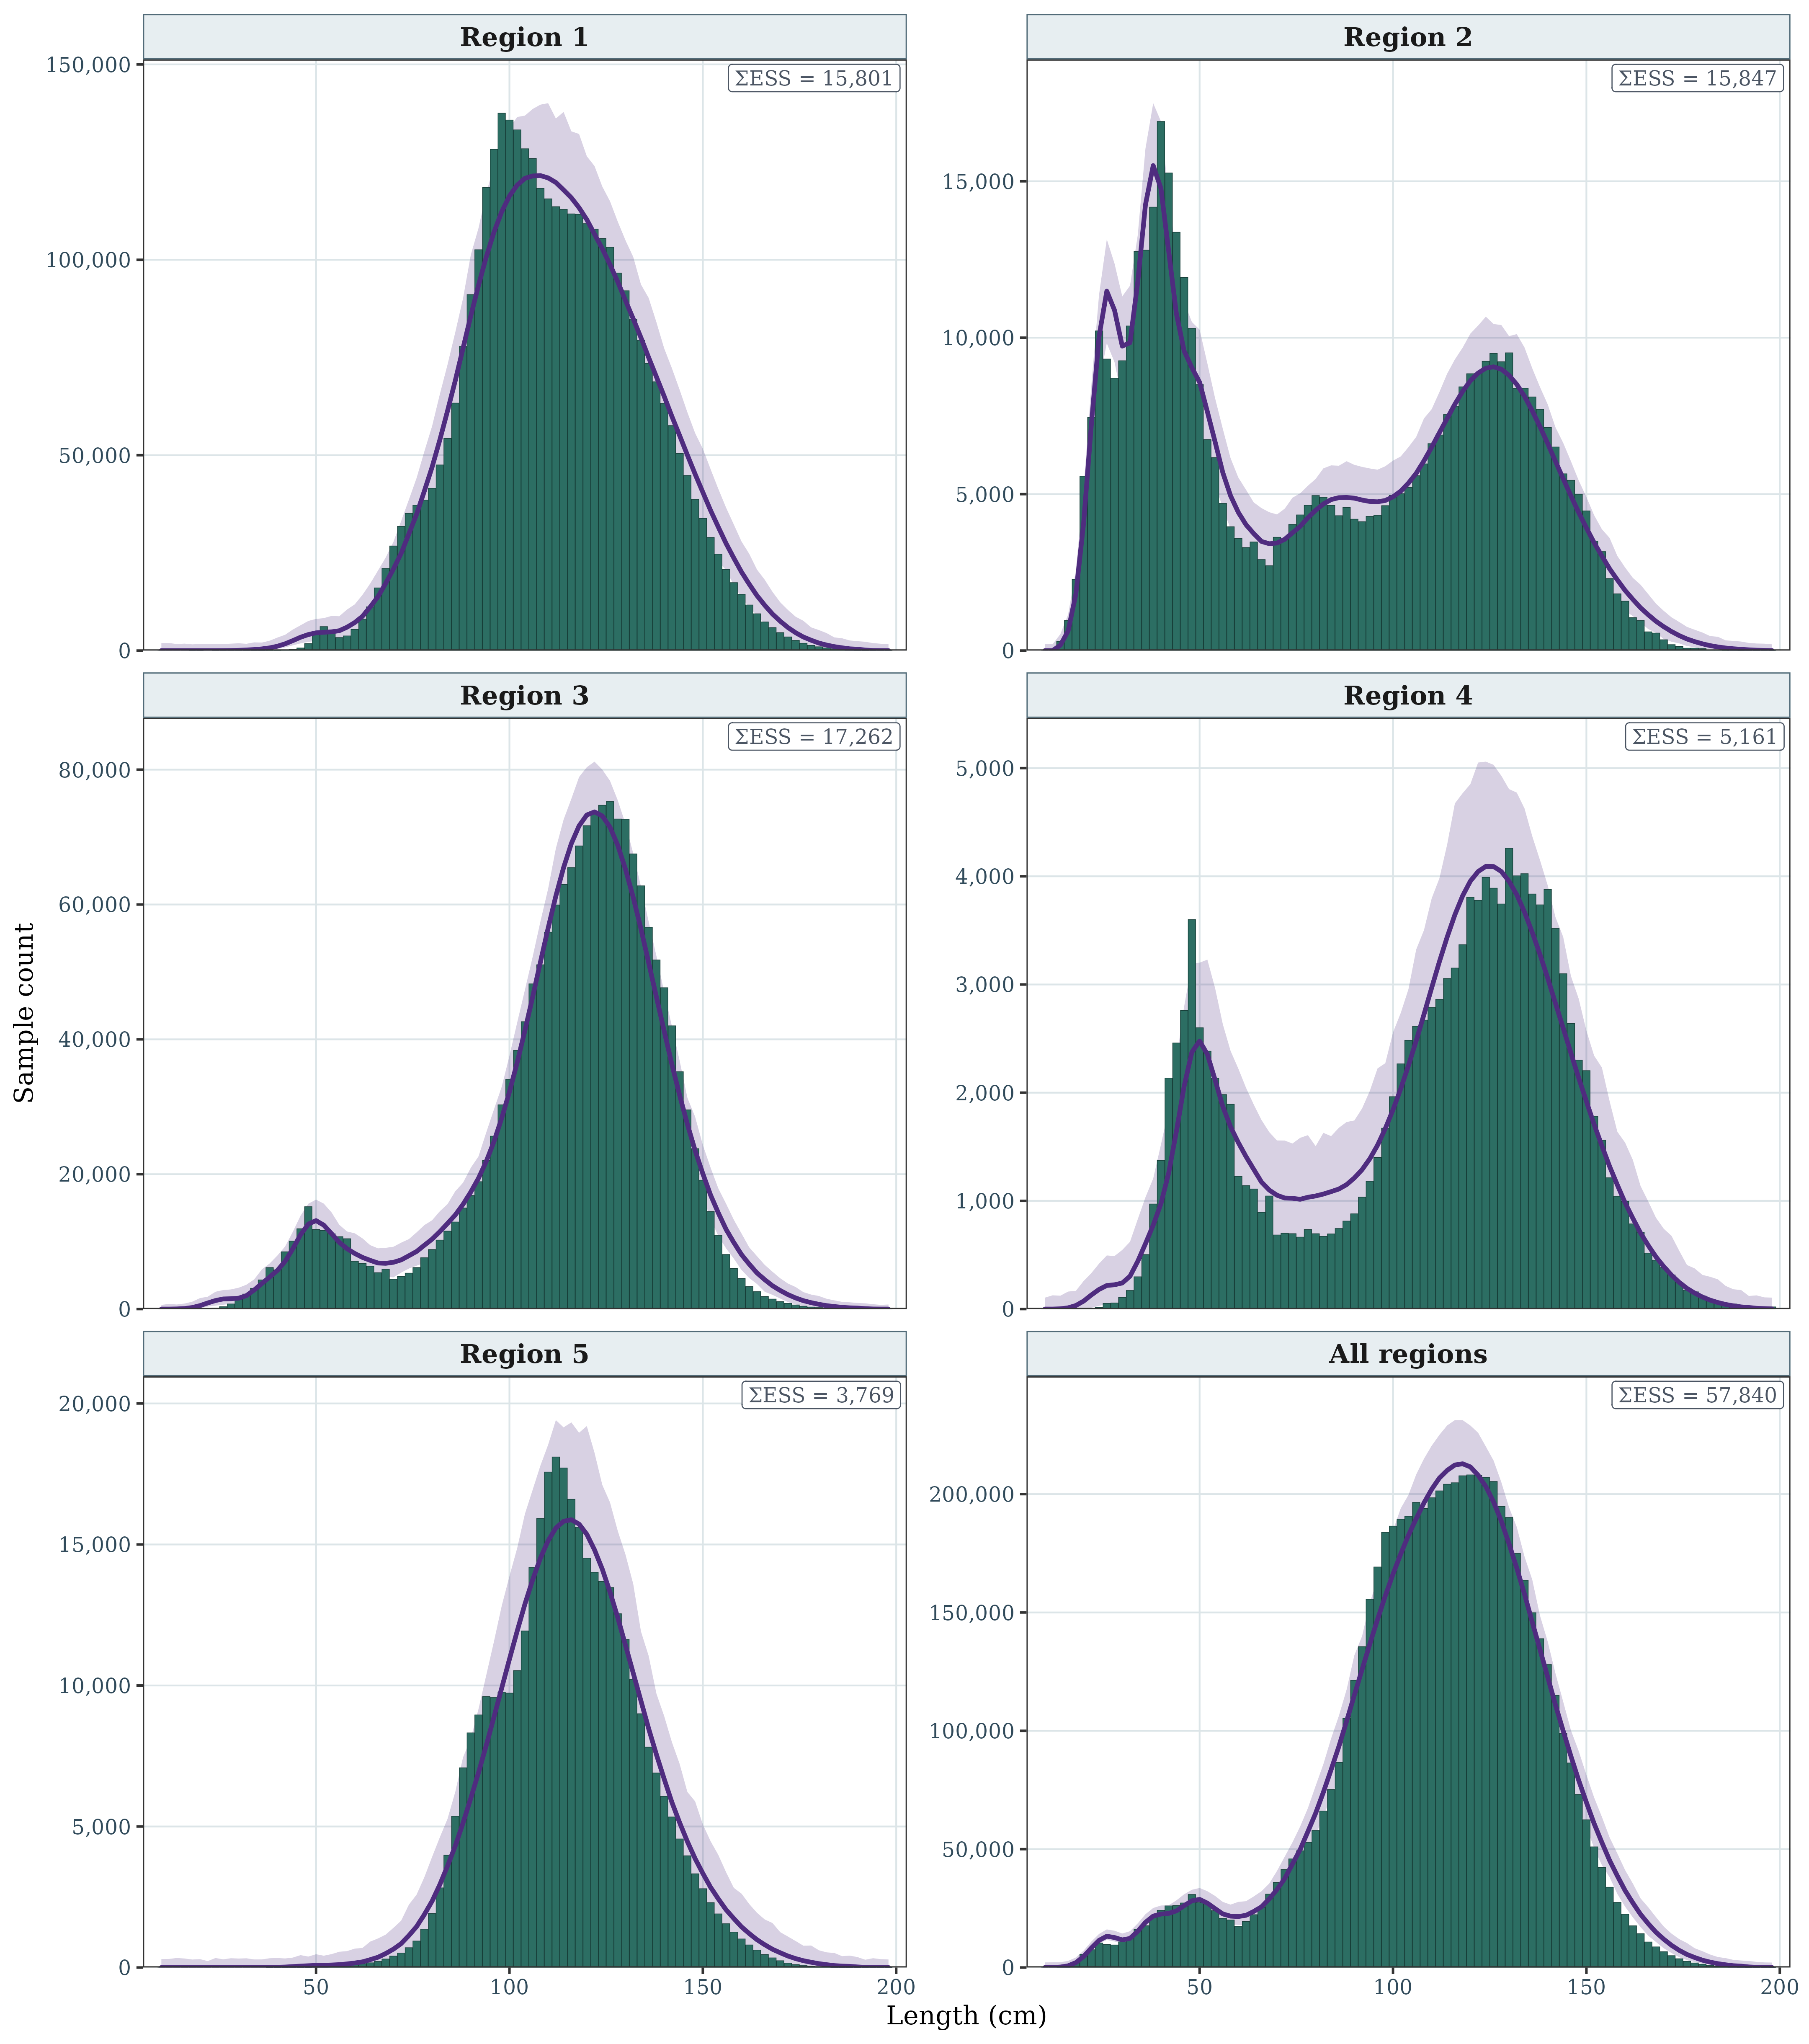
\includegraphics[width=1\linewidth,height=\textheight,keepaspectratio]{figures_new/length-frequency-fit-by-region.png}

}

\caption{\label{fig-length-fit-by-region}Observed (bars) and fitted
(purple lines) length-frequency sample counts aggregated by model region
and over all regions. Shading is the 95\% pointwise conditional
predictive interval for repeated observations under the fitted
Dirichlet--multinomial model; parameter uncertainty is not included. The
top-right \(\Sigma\)ESS is the sum of model-implied incident effective
sample sizes within each panel. Counts are pooled over years and
fisheries for this complementary regional summary. Panel y axes are free
and begin at zero. Open the
\href{https://pacificcommunity.github.io/ofp-sam-bet-2026-diagnostic/bet-2026-diagnostic-report.html}{interactive
diagnostic report} for fishery- and year-level selections.}

\end{figure}\DIFaddend %

\DIFdelbegin %DIFDELCMD < \begin{figure}[H]
%DIFDELCMD <

%DIFDELCMD < \centering{
%DIFDELCMD <

%DIFDELCMD < 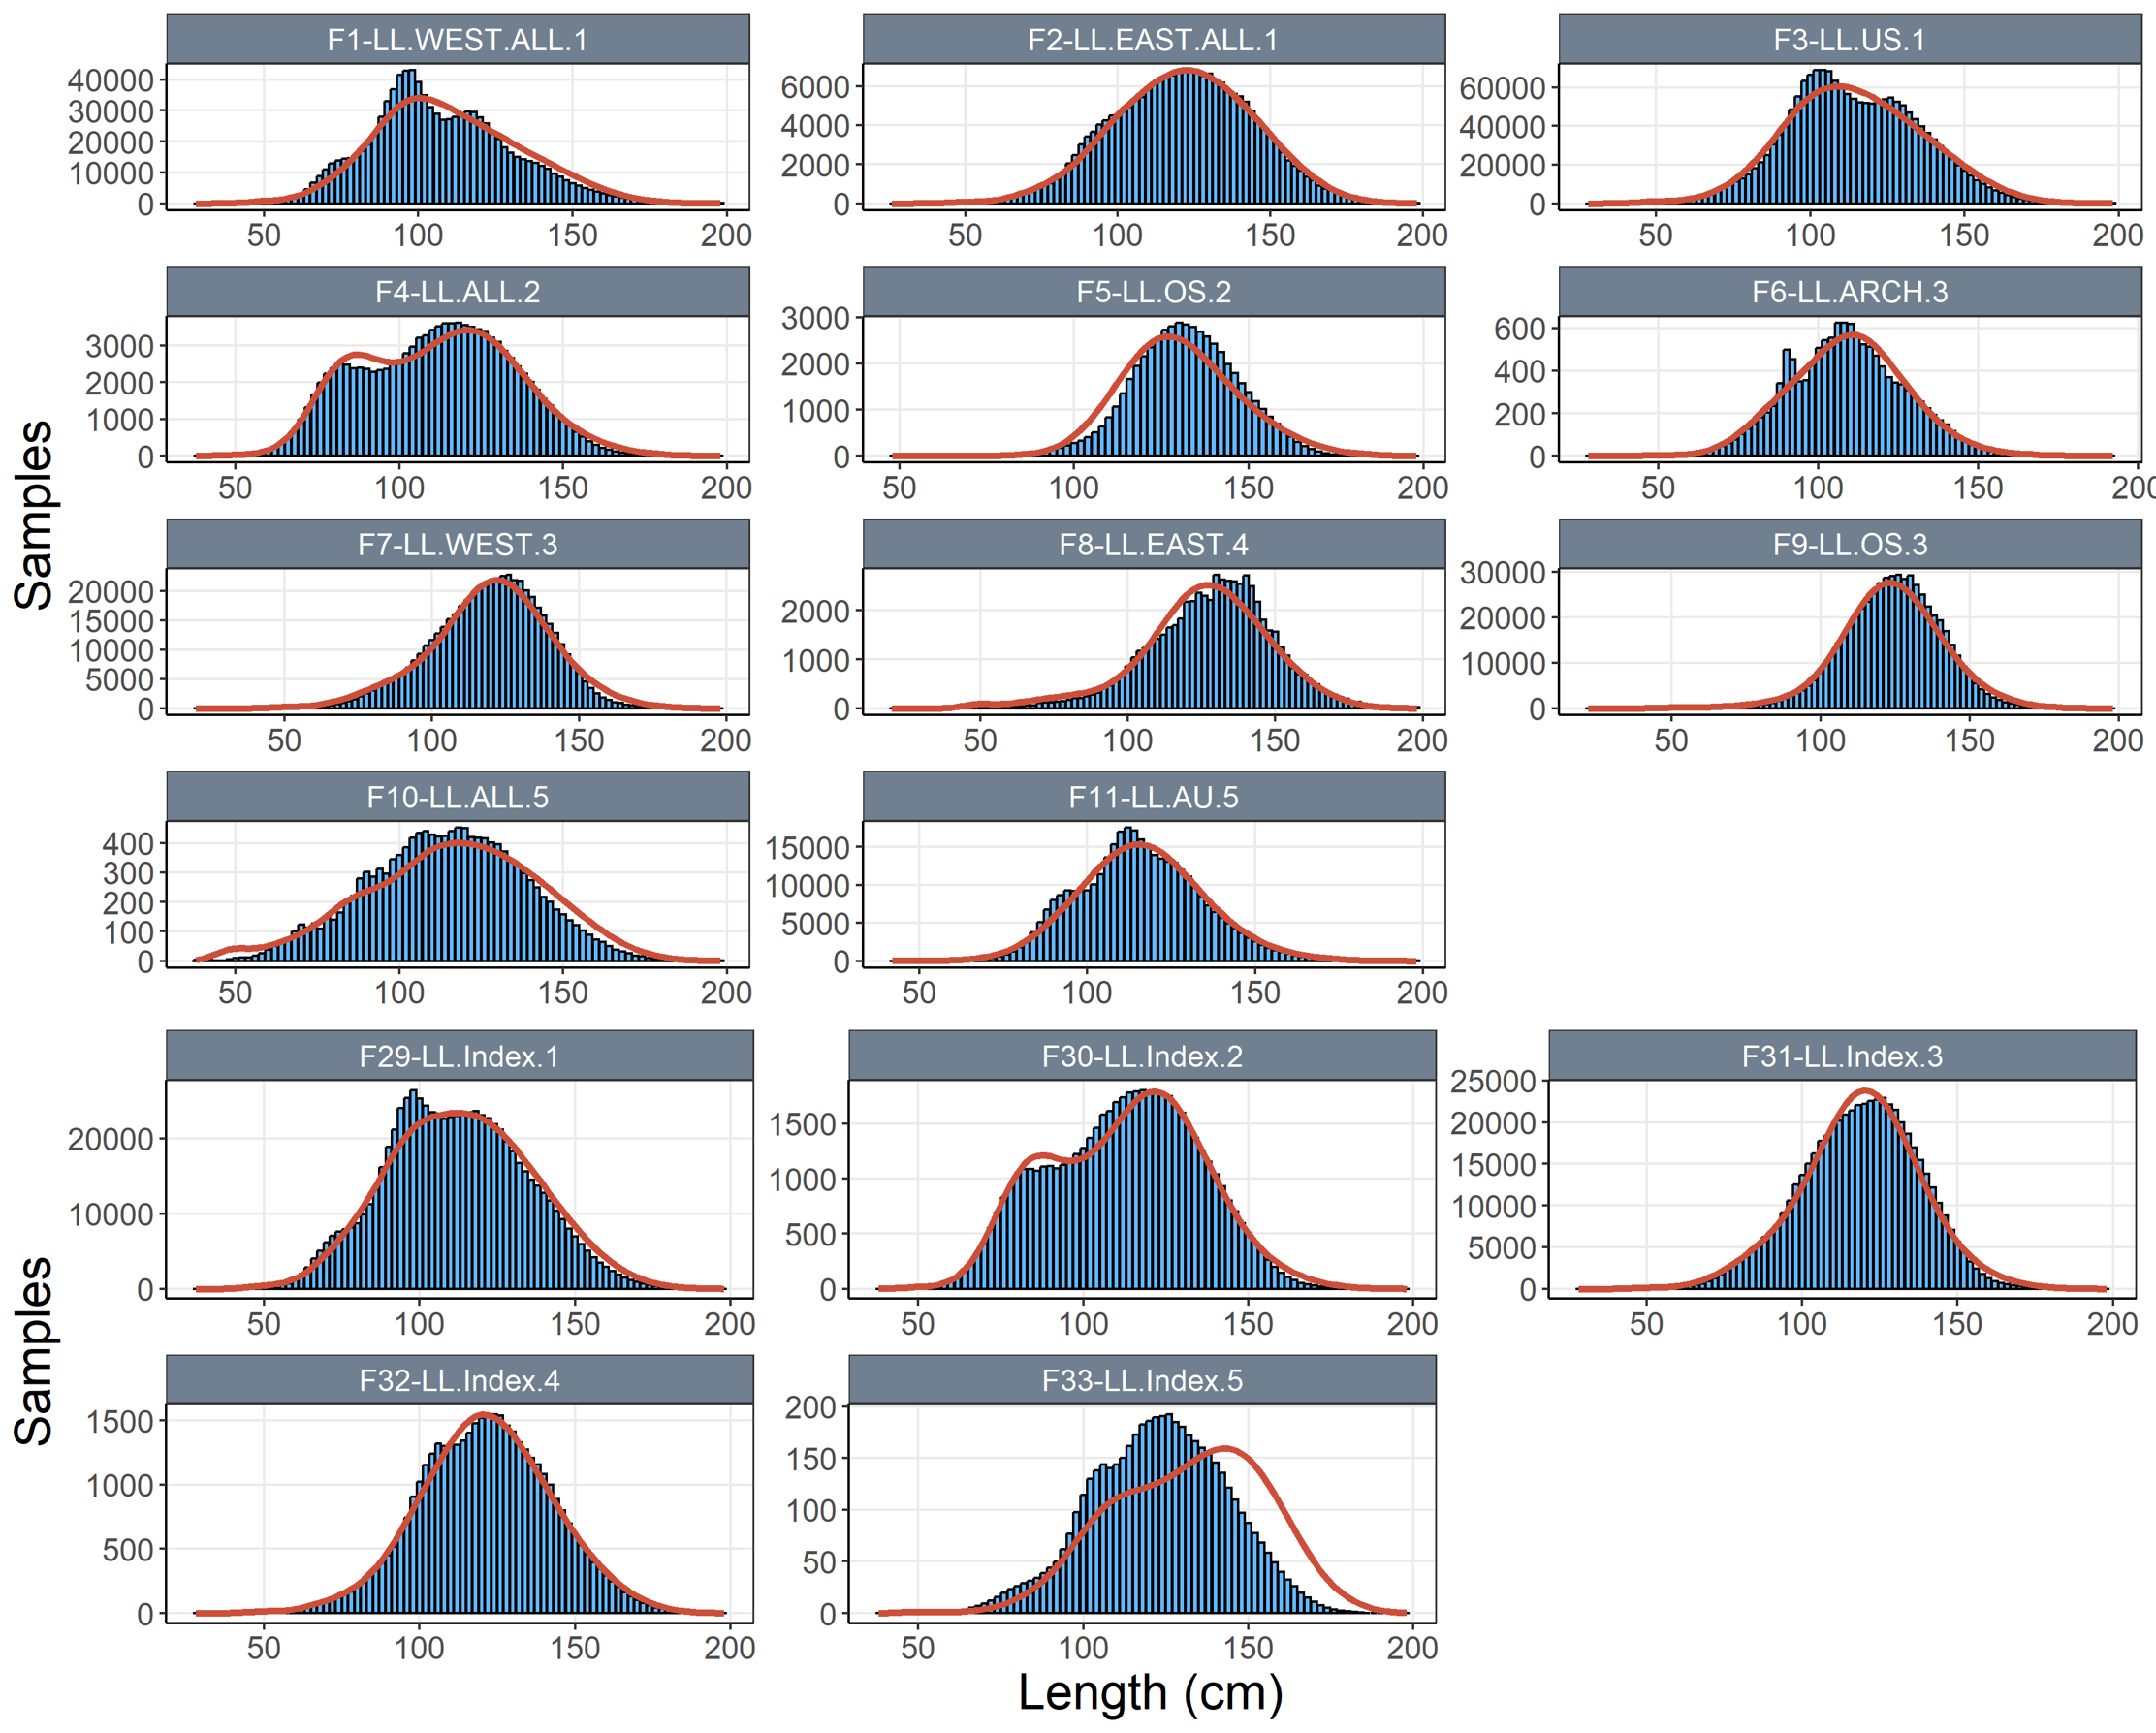
\includegraphics[width=1\linewidth,height=\textheight,keepaspectratio]{figures/length_fit_aggregated_ll.png}
%DIFDELCMD <

%DIFDELCMD < }
%DIFDELCMD <

%DIFDELCMD < \caption{\label{fig-length-fit-aggregated-ll}Composite (all time periods
%DIFDELCMD < combined) observed (blue histograms) and predicted (red line) length
%DIFDELCMD < frequency for fisheries with length frequency data for longline
%DIFDELCMD < extraction and index fisheries in the 2026 diagnostic model.}
%DIFDELCMD <

%DIFDELCMD < \end{figure}%%%
\DIFdelend \DIFaddbegin \begin{figure}[H]

\centering{

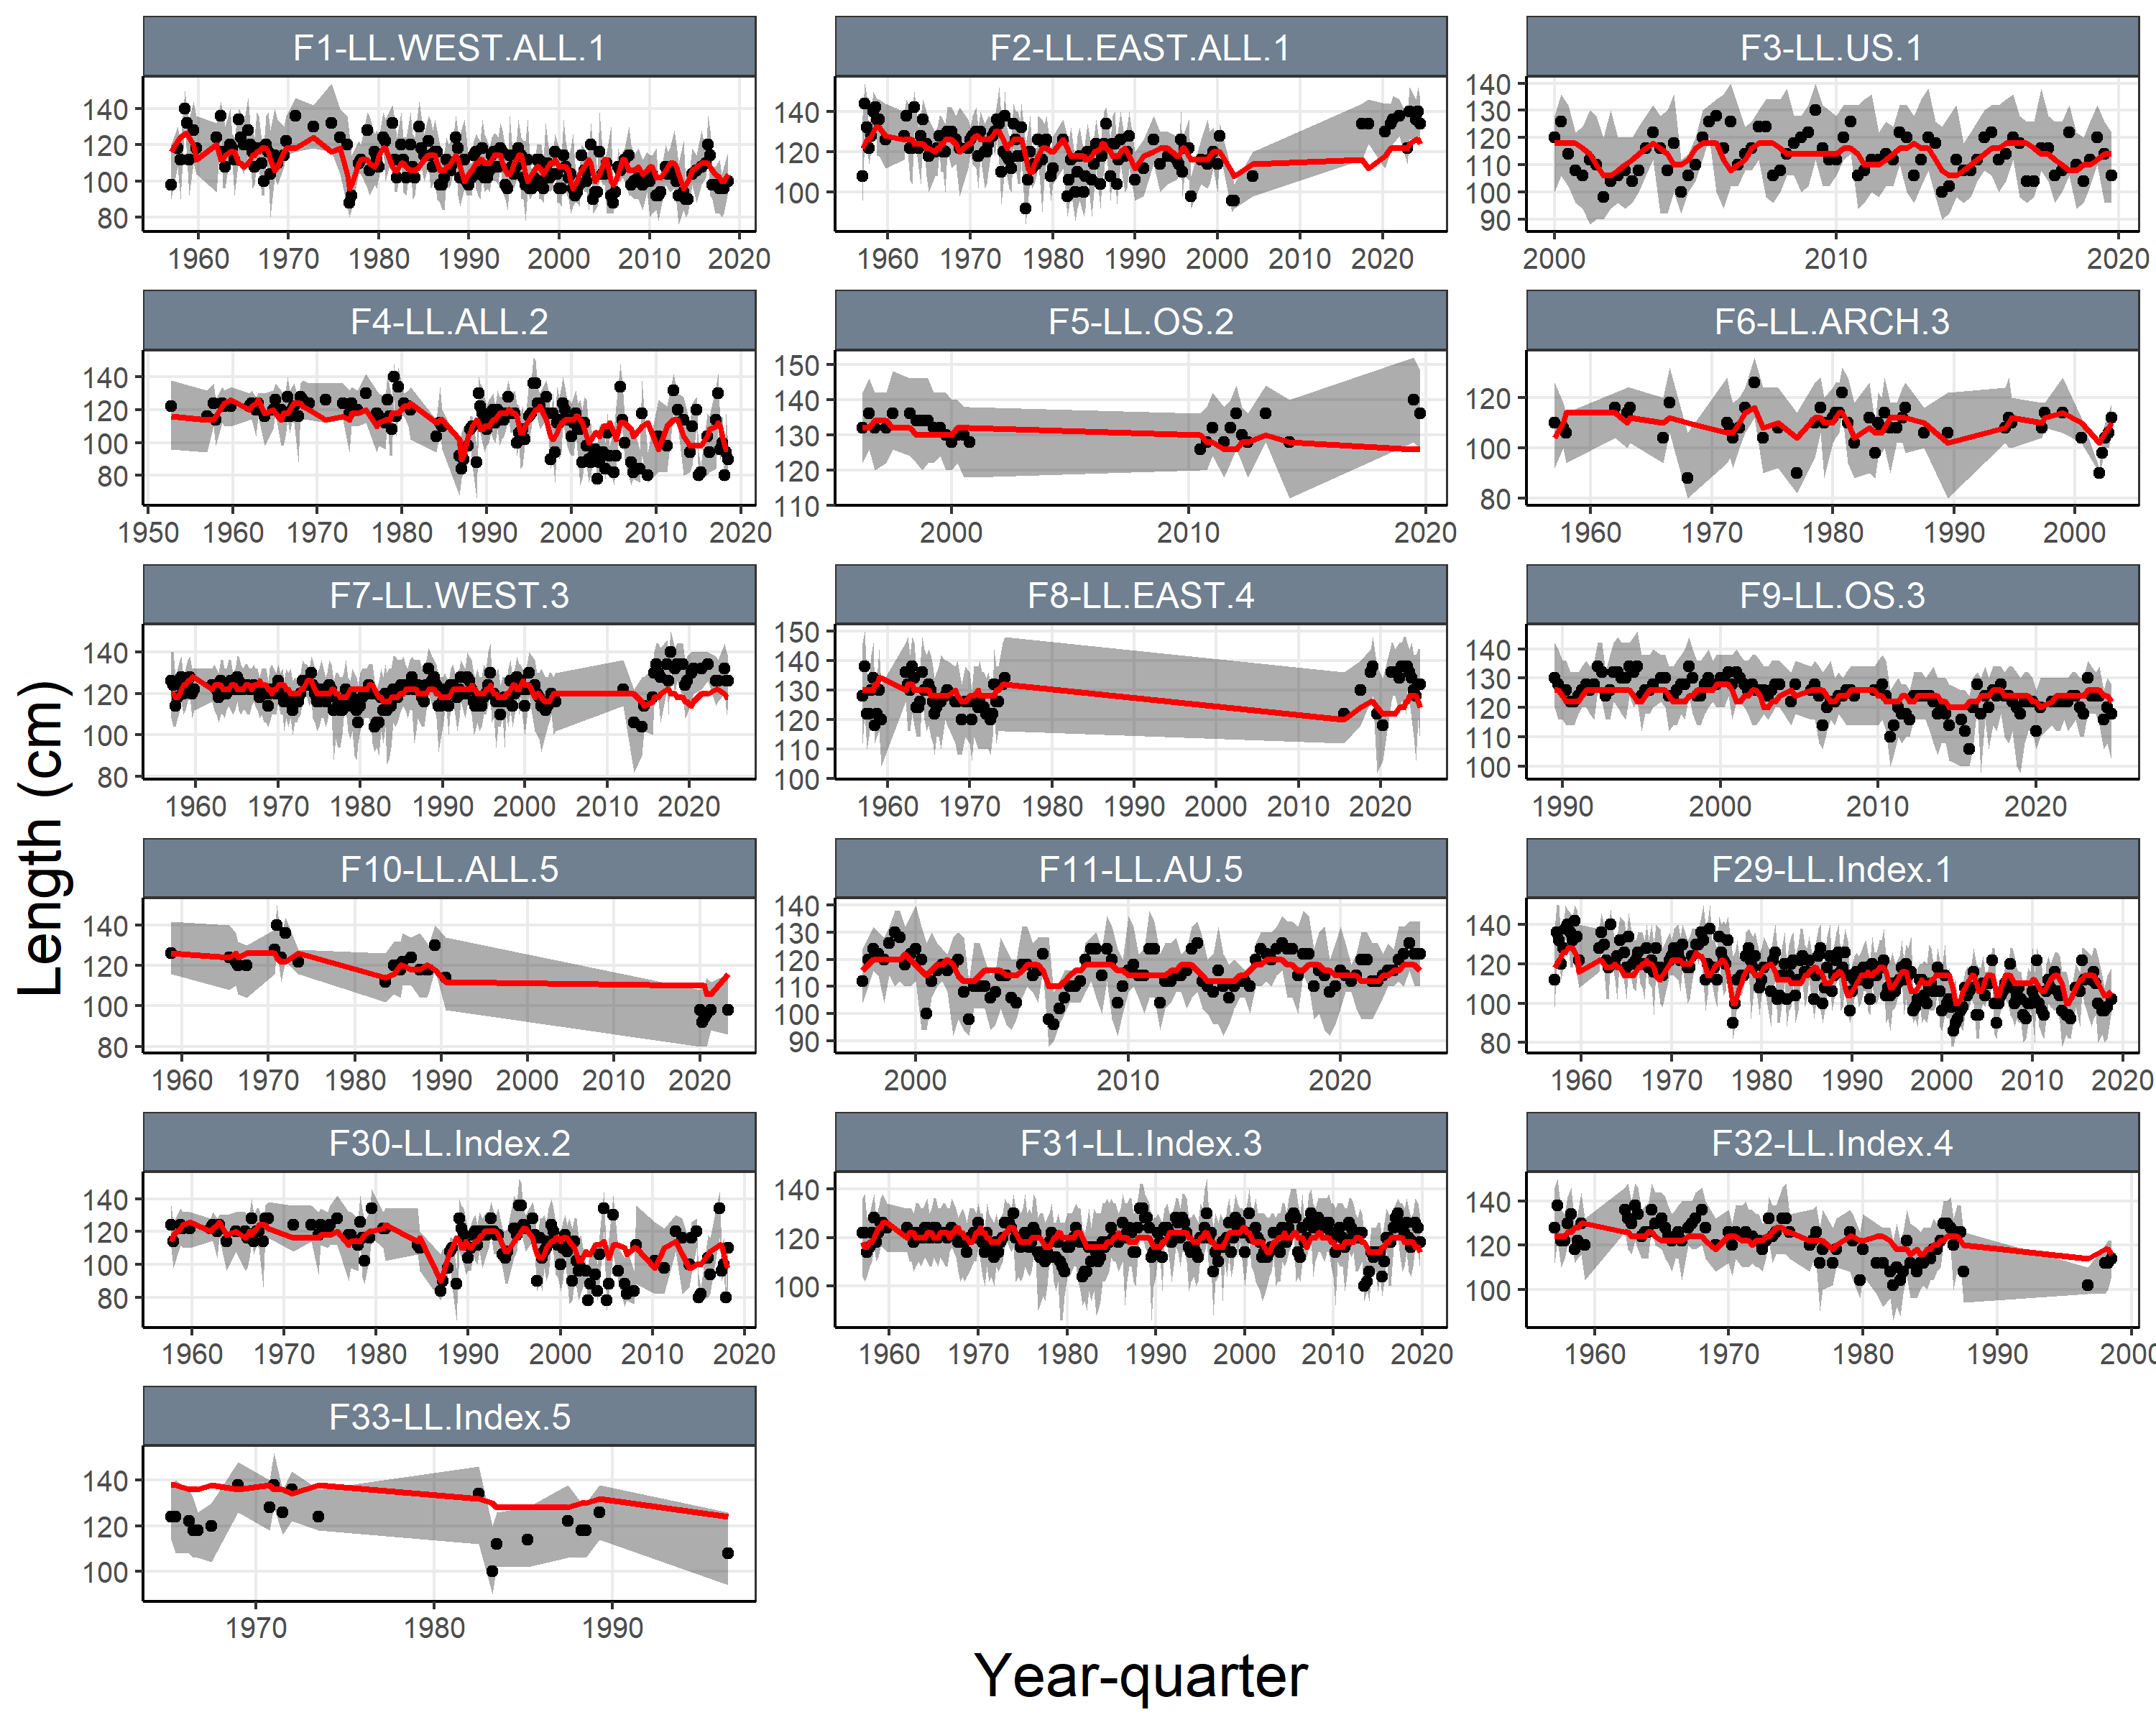
\includegraphics[width=1\linewidth,height=\textheight,keepaspectratio]{figures/length_fit_time_series_ll.png}

}

\caption{\label{fig-length-fit-timeseries-ll}Observed (red points) and
predicted (red line) median fish lengths (FL, cm) for the longline
fisheries for the 2026 diagnostic model. The uncertainty intervals (gray
shading) represent the values encompassed by the 25\% and 75\%
quantiles. Sampling data are by quarter and only length samples with
more than 250 fish per quarter/fishery strata are plotted.}

\end{figure}\DIFaddend %

\DIFdelbegin %DIFDELCMD < \begin{figure}[H]
%DIFDELCMD <

%DIFDELCMD < \centering{
%DIFDELCMD <

%DIFDELCMD < 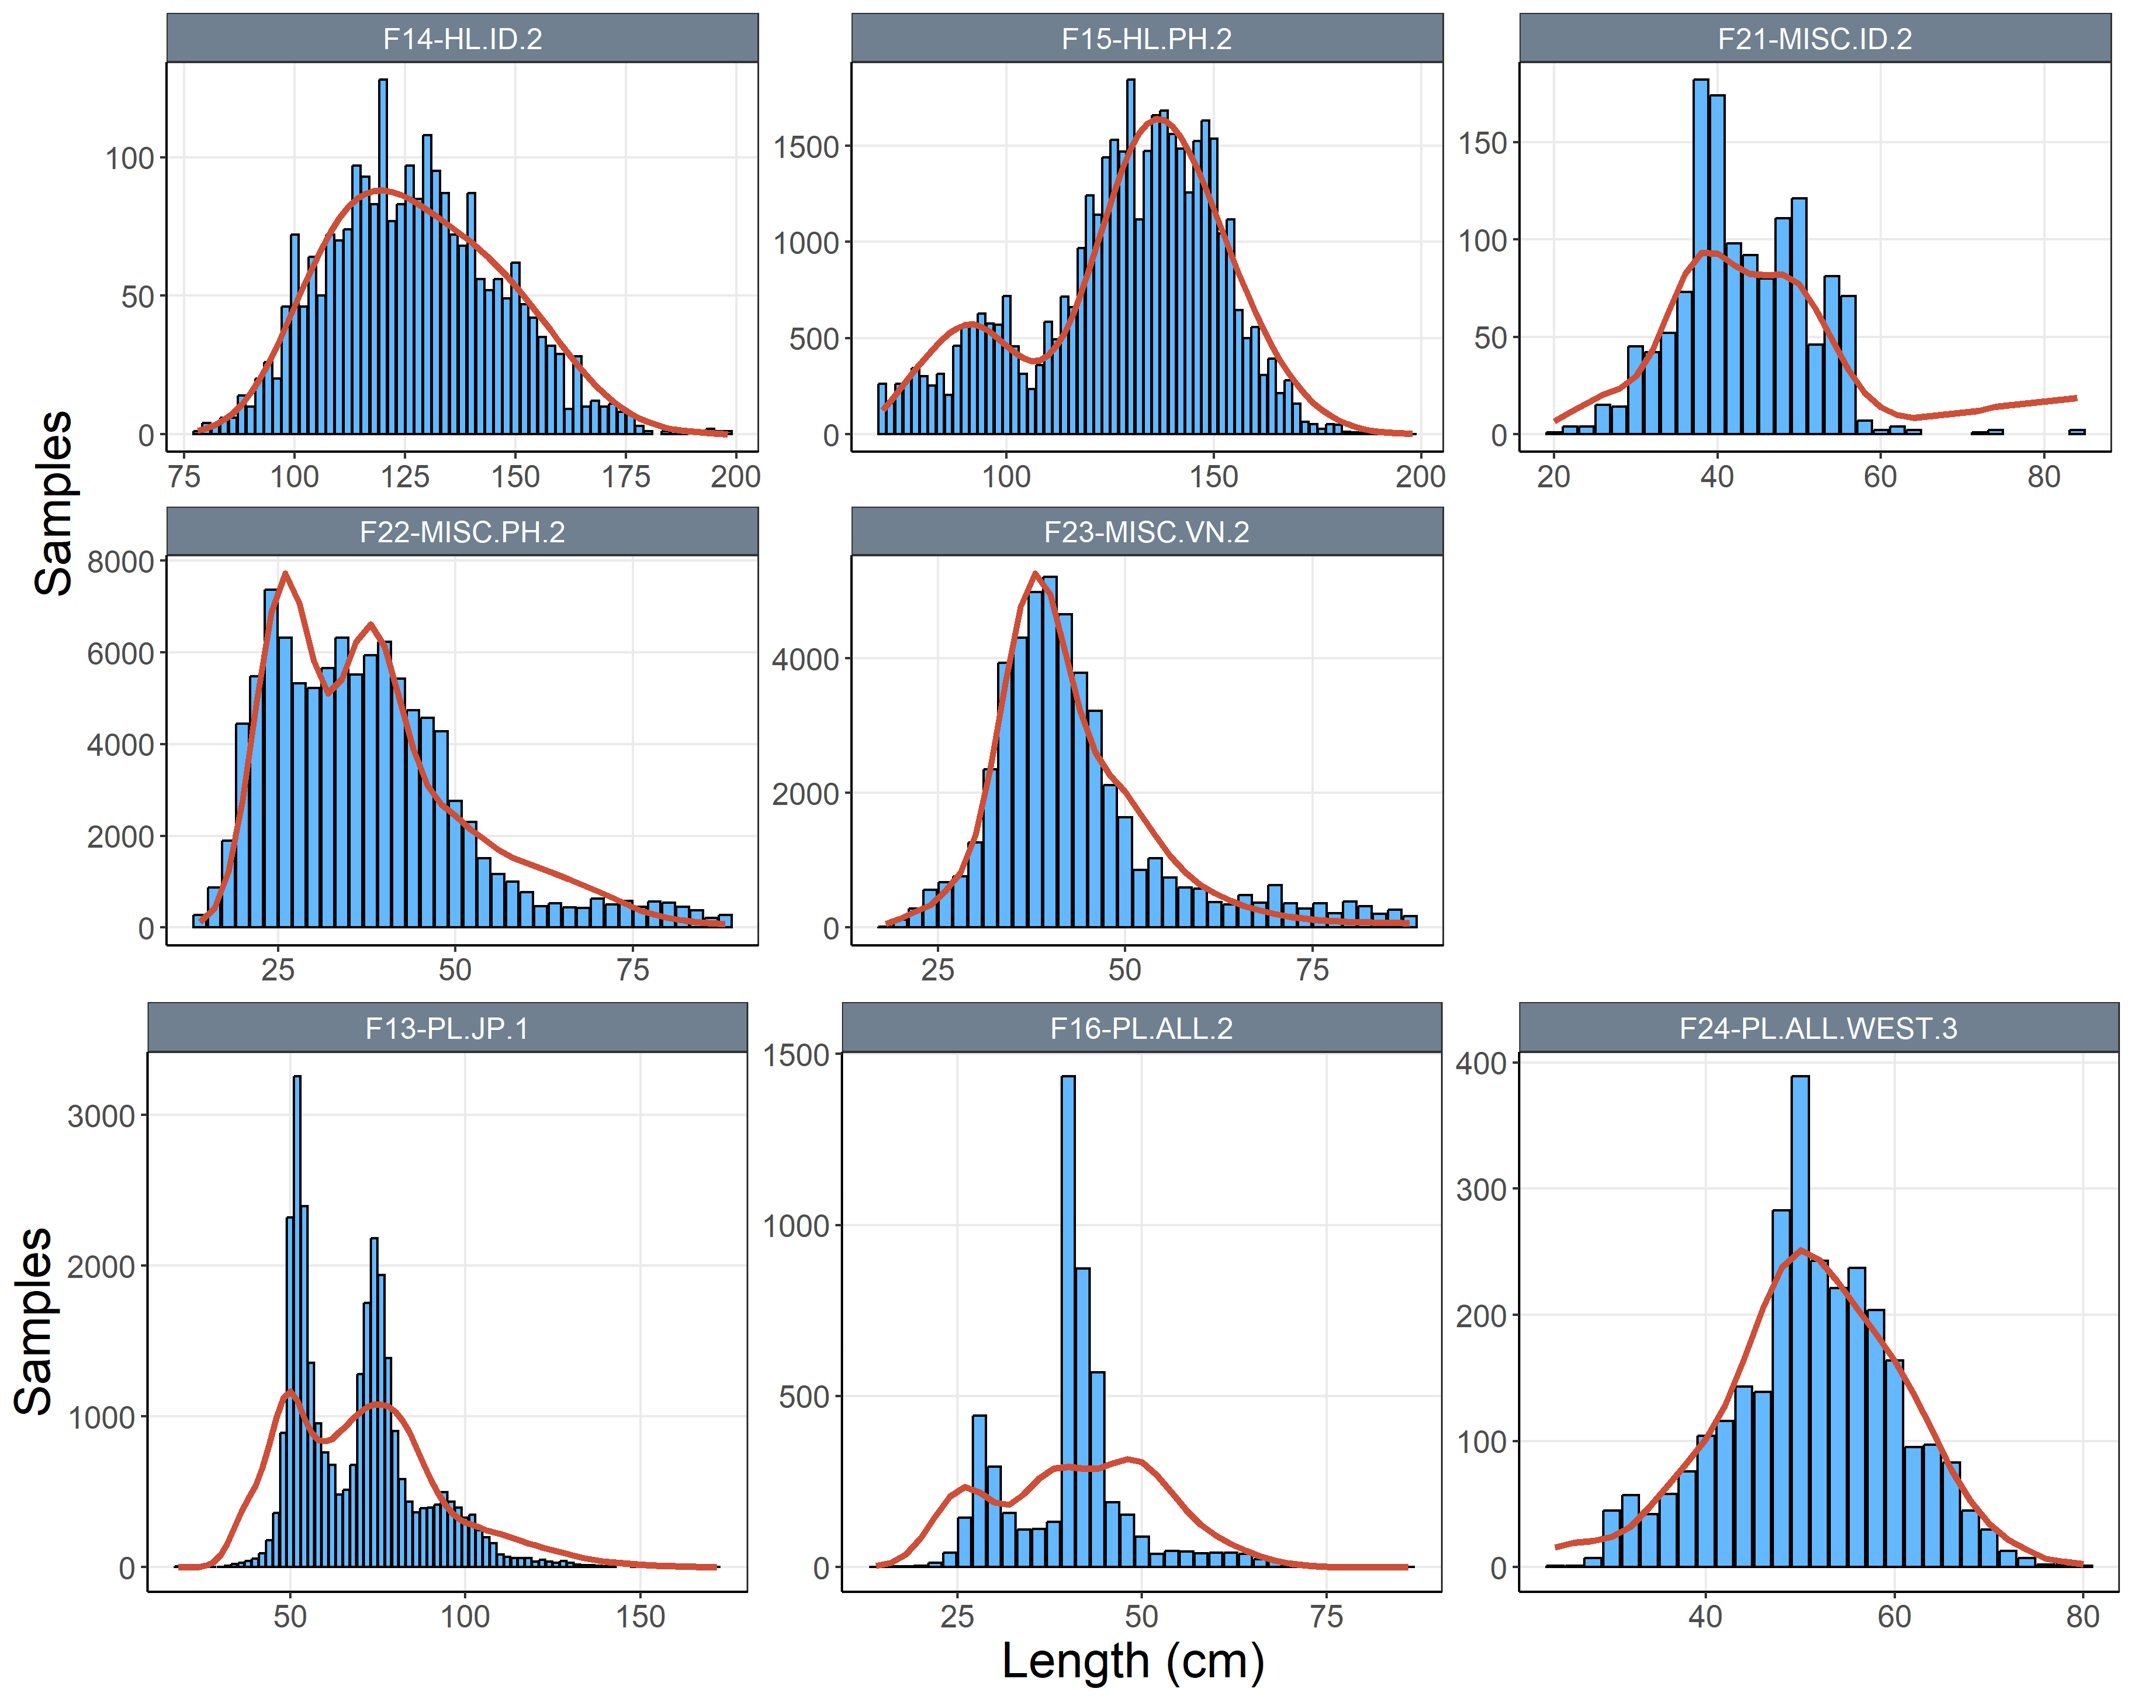
\includegraphics[width=1\linewidth,height=\textheight,keepaspectratio]{figures/length_fit_aggregated_dompl.png}
%DIFDELCMD <

%DIFDELCMD < }
%DIFDELCMD <

%DIFDELCMD < \caption{\label{fig-length-fit-aggregated-dompl}Composite (all time
%DIFDELCMD < periods combined) observed (blue histograms) and predicted (red line)
%DIFDELCMD < length frequency for fisheries with length frequency data for domestic,
%DIFDELCMD < handline and pole and line fisheries in the 2026 diagnostic model.}
%DIFDELCMD <

%DIFDELCMD < \end{figure}%%%
\DIFdelend \DIFaddbegin \begin{figure}[H]

\centering{

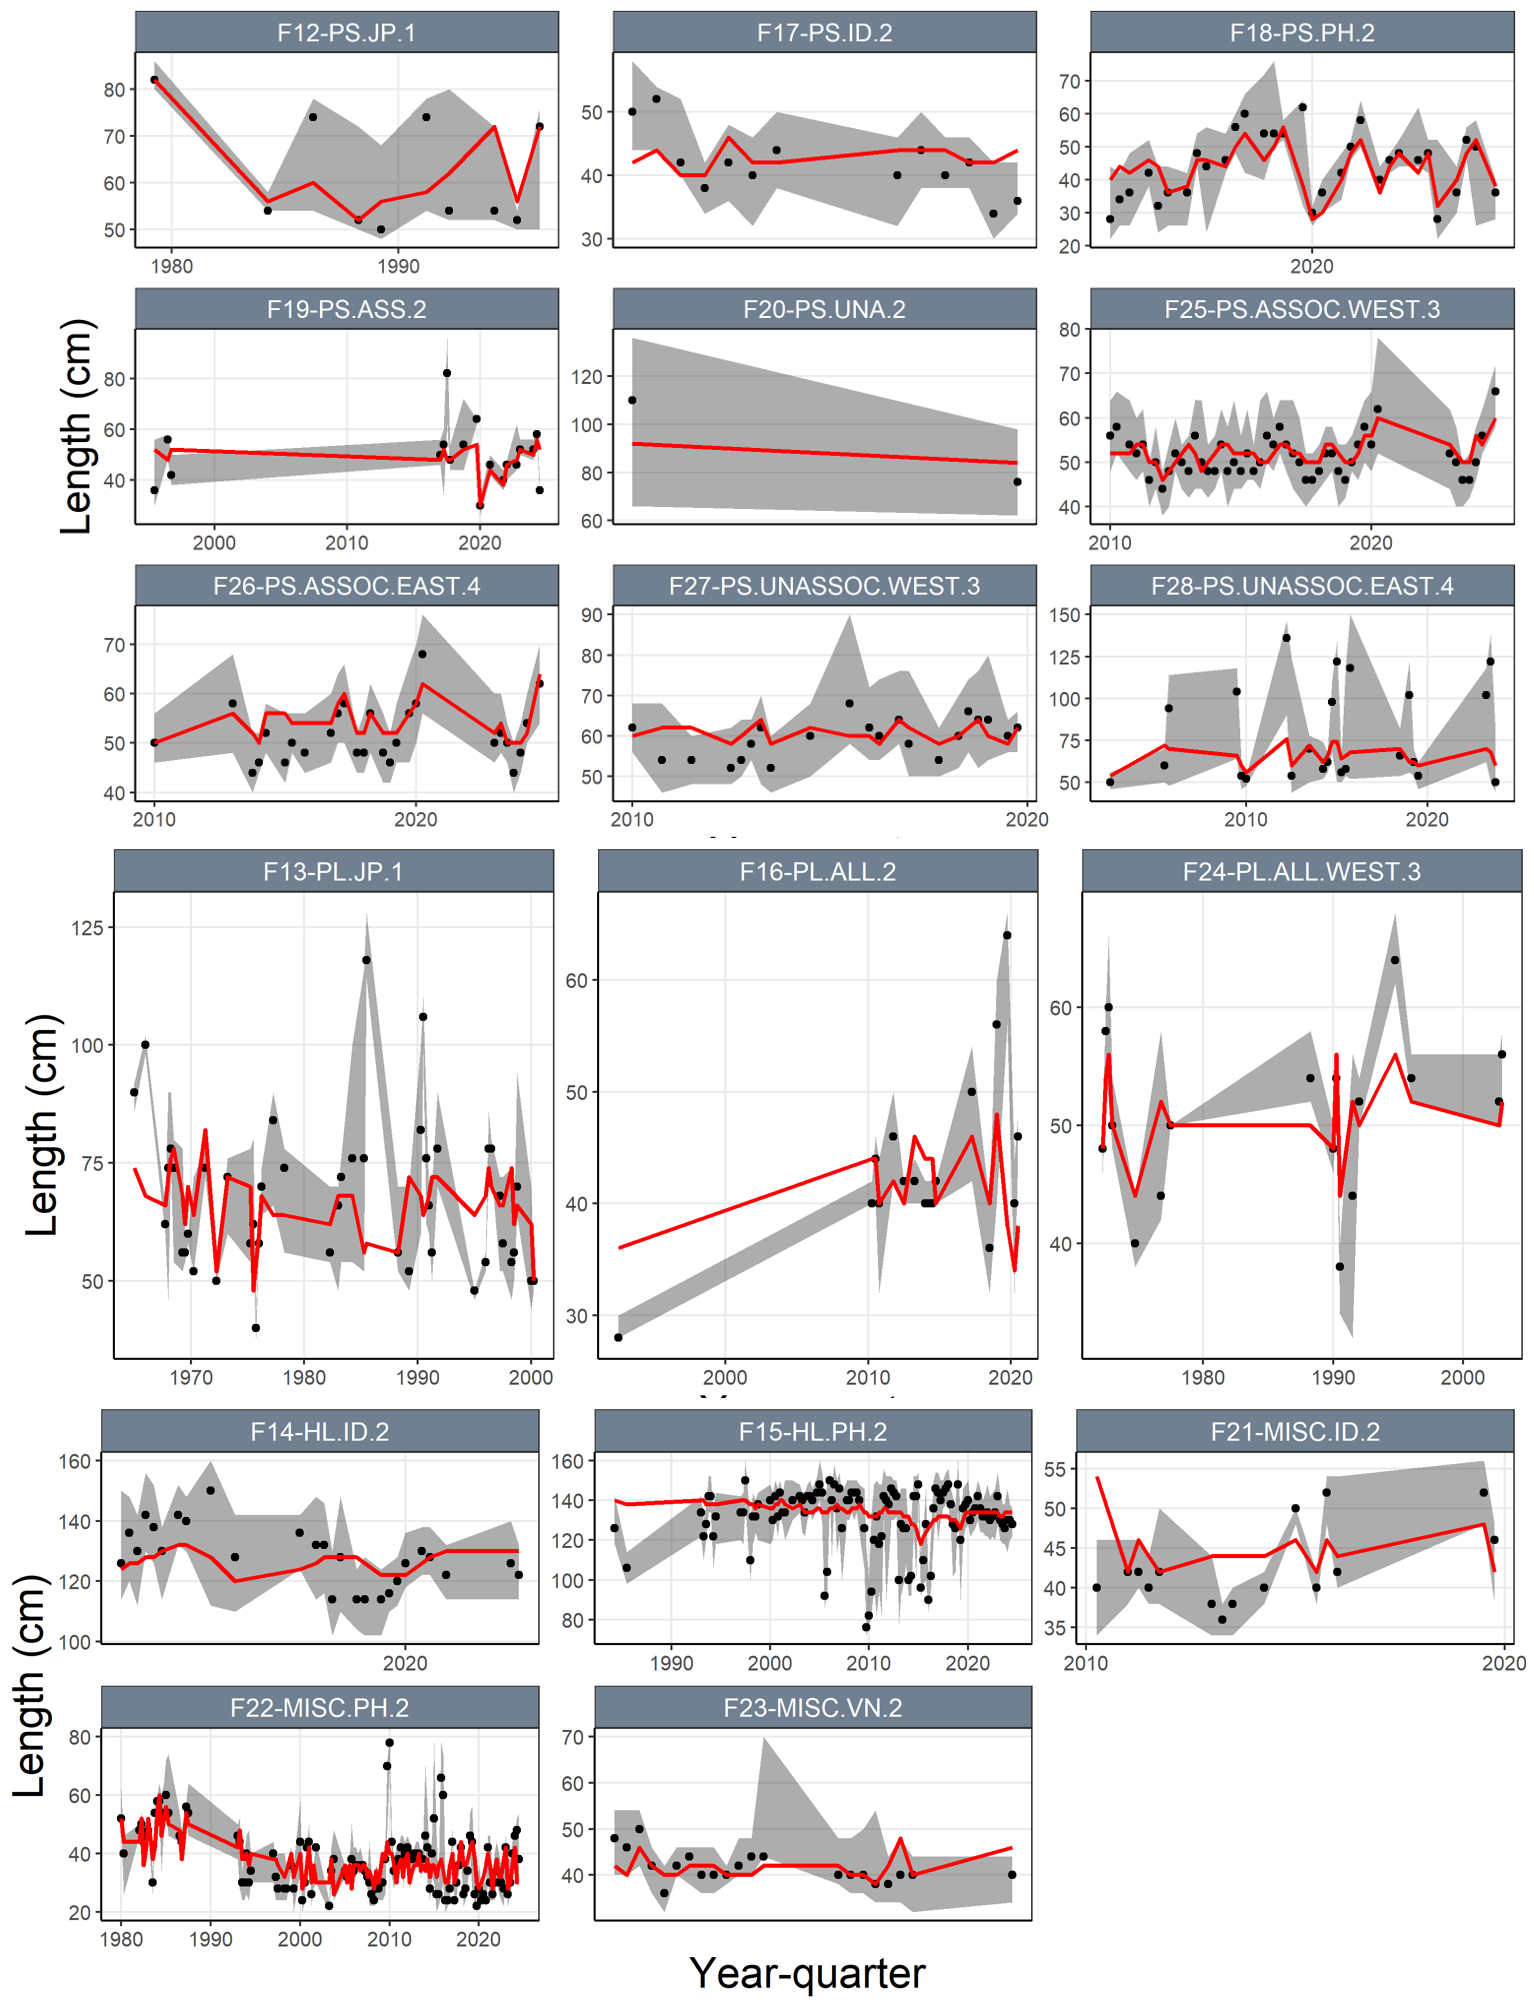
\includegraphics[width=0.75\linewidth,height=\textheight,keepaspectratio]{figures/length_fit_time_series_other.png}

}

\caption{\label{fig-length-fit-timeseries-other}Observed (red points)
and predicted (red line) median fish lengths (FL, cm) for the other
fisheries for the 2026 diagnostic model. The uncertainty intervals (gray
shading) represent the values encompassed by the 25\% and 75\%
quantiles. Sampling data are by quarter and only length samples with
more than 100 fish per quarter/fishery strata are plotted.}

\end{figure}\DIFaddend %

\DIFdelbegin %DIFDELCMD < \begin{figure}[H]
%DIFDELCMD <

%DIFDELCMD < \centering{
%DIFDELCMD <

%DIFDELCMD < 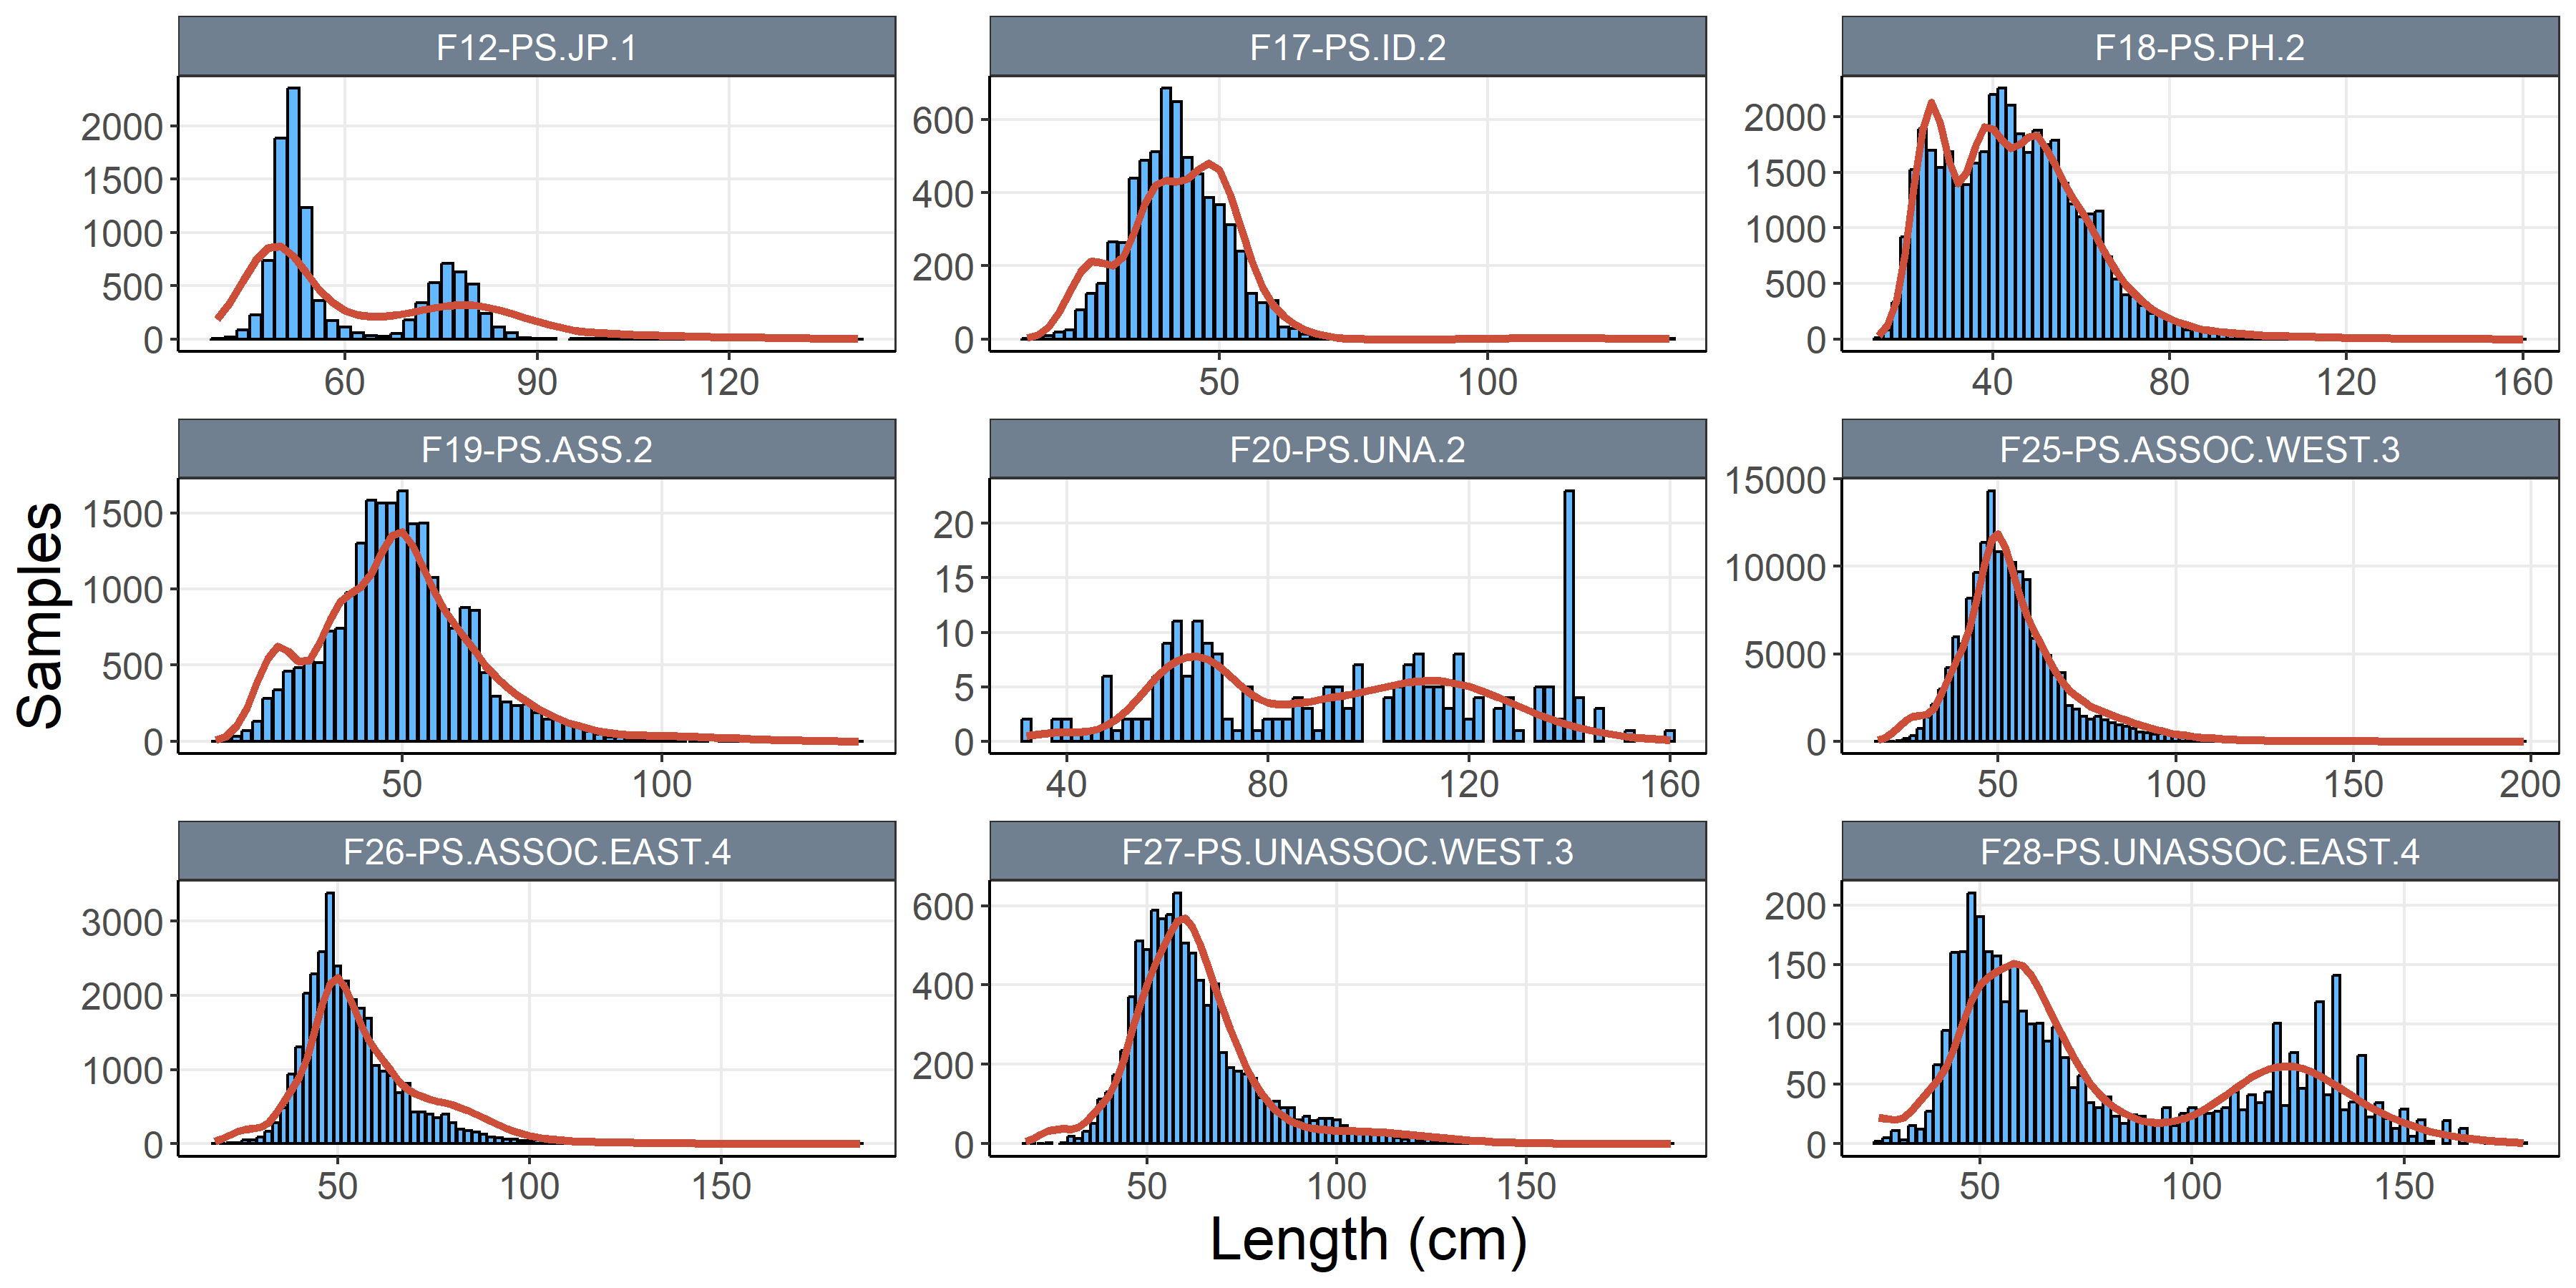
\includegraphics[width=1\linewidth,height=\textheight,keepaspectratio]{figures/length_fit_aggregated_ps.png}
%DIFDELCMD <

%DIFDELCMD < }
%DIFDELCMD <

%DIFDELCMD < \caption{\label{fig-length-fit-aggregated-ps}Composite (all time periods
%DIFDELCMD < combined) observed (blue histograms) and predicted (red line) length
%DIFDELCMD < frequency for fisheries with length frequency data for purse seine
%DIFDELCMD < fisheries in the 2026 diagnostic model.}
%DIFDELCMD <

%DIFDELCMD < \end{figure}%%%
\DIFdelend \DIFaddbegin \begin{figure}[H]

\centering{

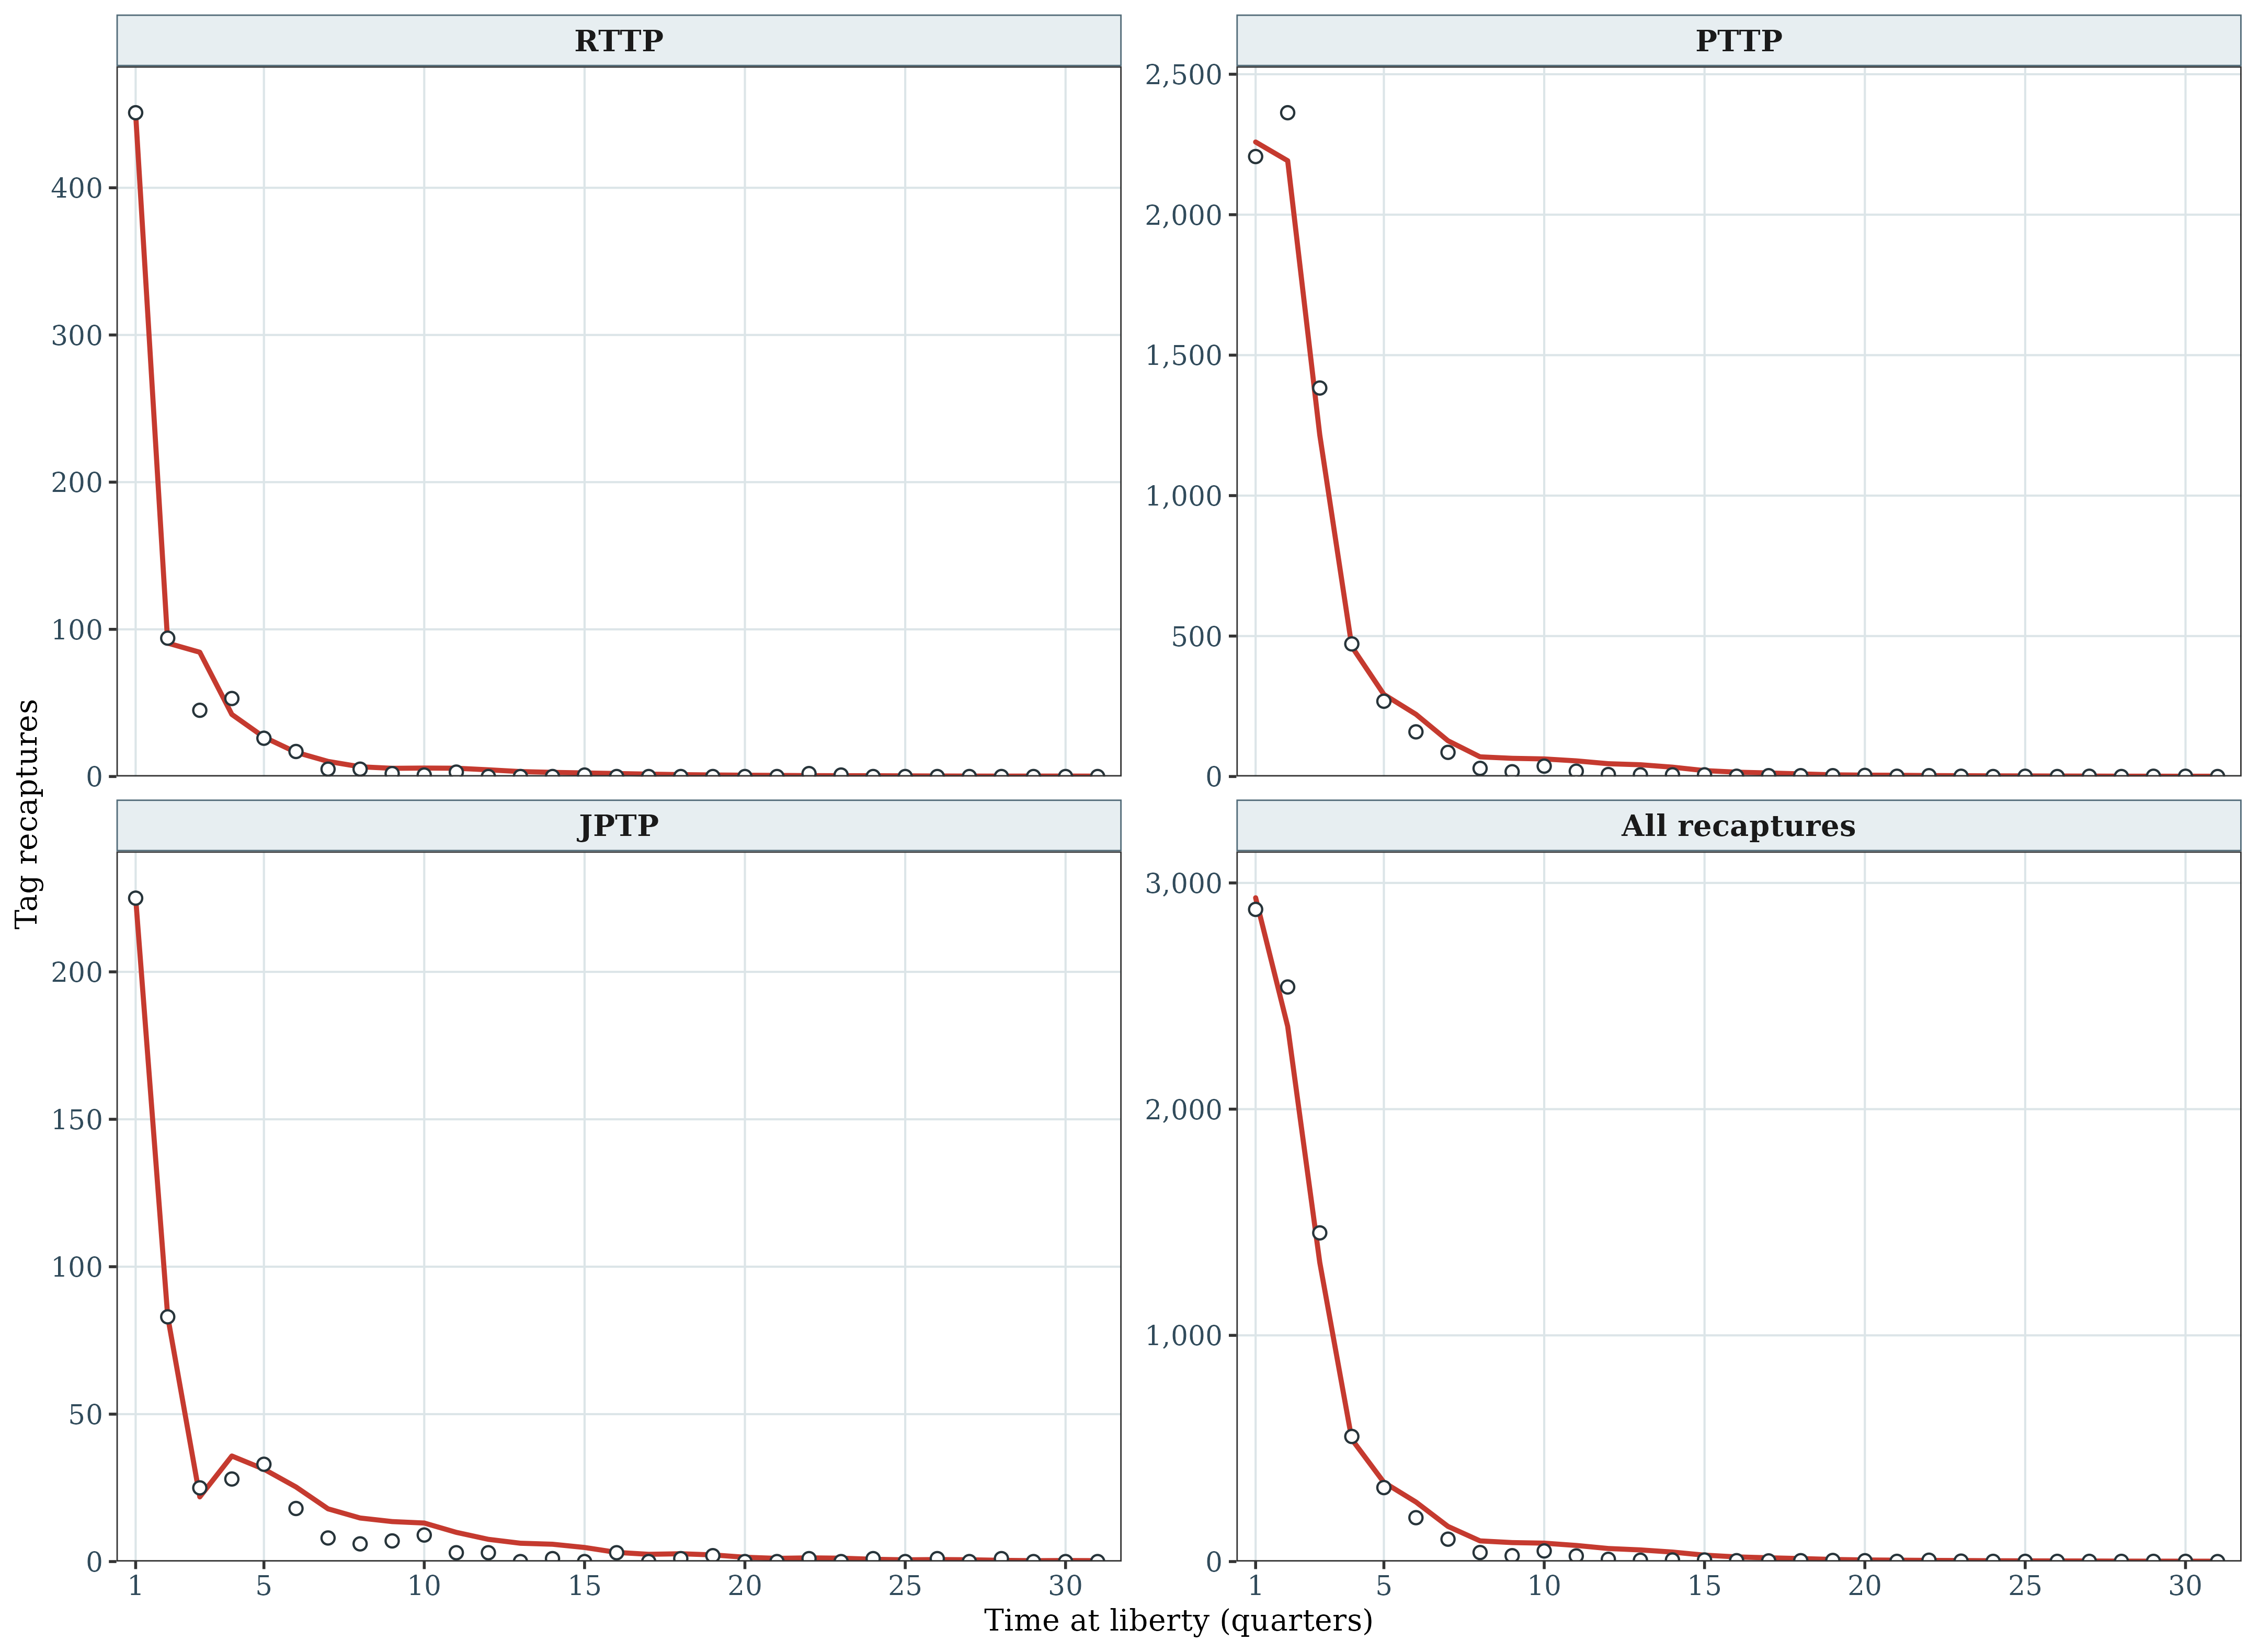
\includegraphics[width=1\linewidth,height=\textheight,keepaspectratio]{figures_new/tag-attrition-by-program.png}

}

\caption{\label{fig-tag-attrition-programmes}\label{fig-tag-attrition-all}Observed (black points) and
model-predicted (red line) tag recaptures by time at liberty in quarters
for RTTP, PTTP, JPTP and all recaptures. Programme predictions apply
MFCL's premixing reporting-rate rule and reconcile to the official
all-recapture diagnostic within its printed precision.}

\end{figure}\DIFaddend %

\DIFdelbegin %DIFDELCMD < \begin{figure}[H]
%DIFDELCMD <

%DIFDELCMD < \centering{
%DIFDELCMD <

%DIFDELCMD < 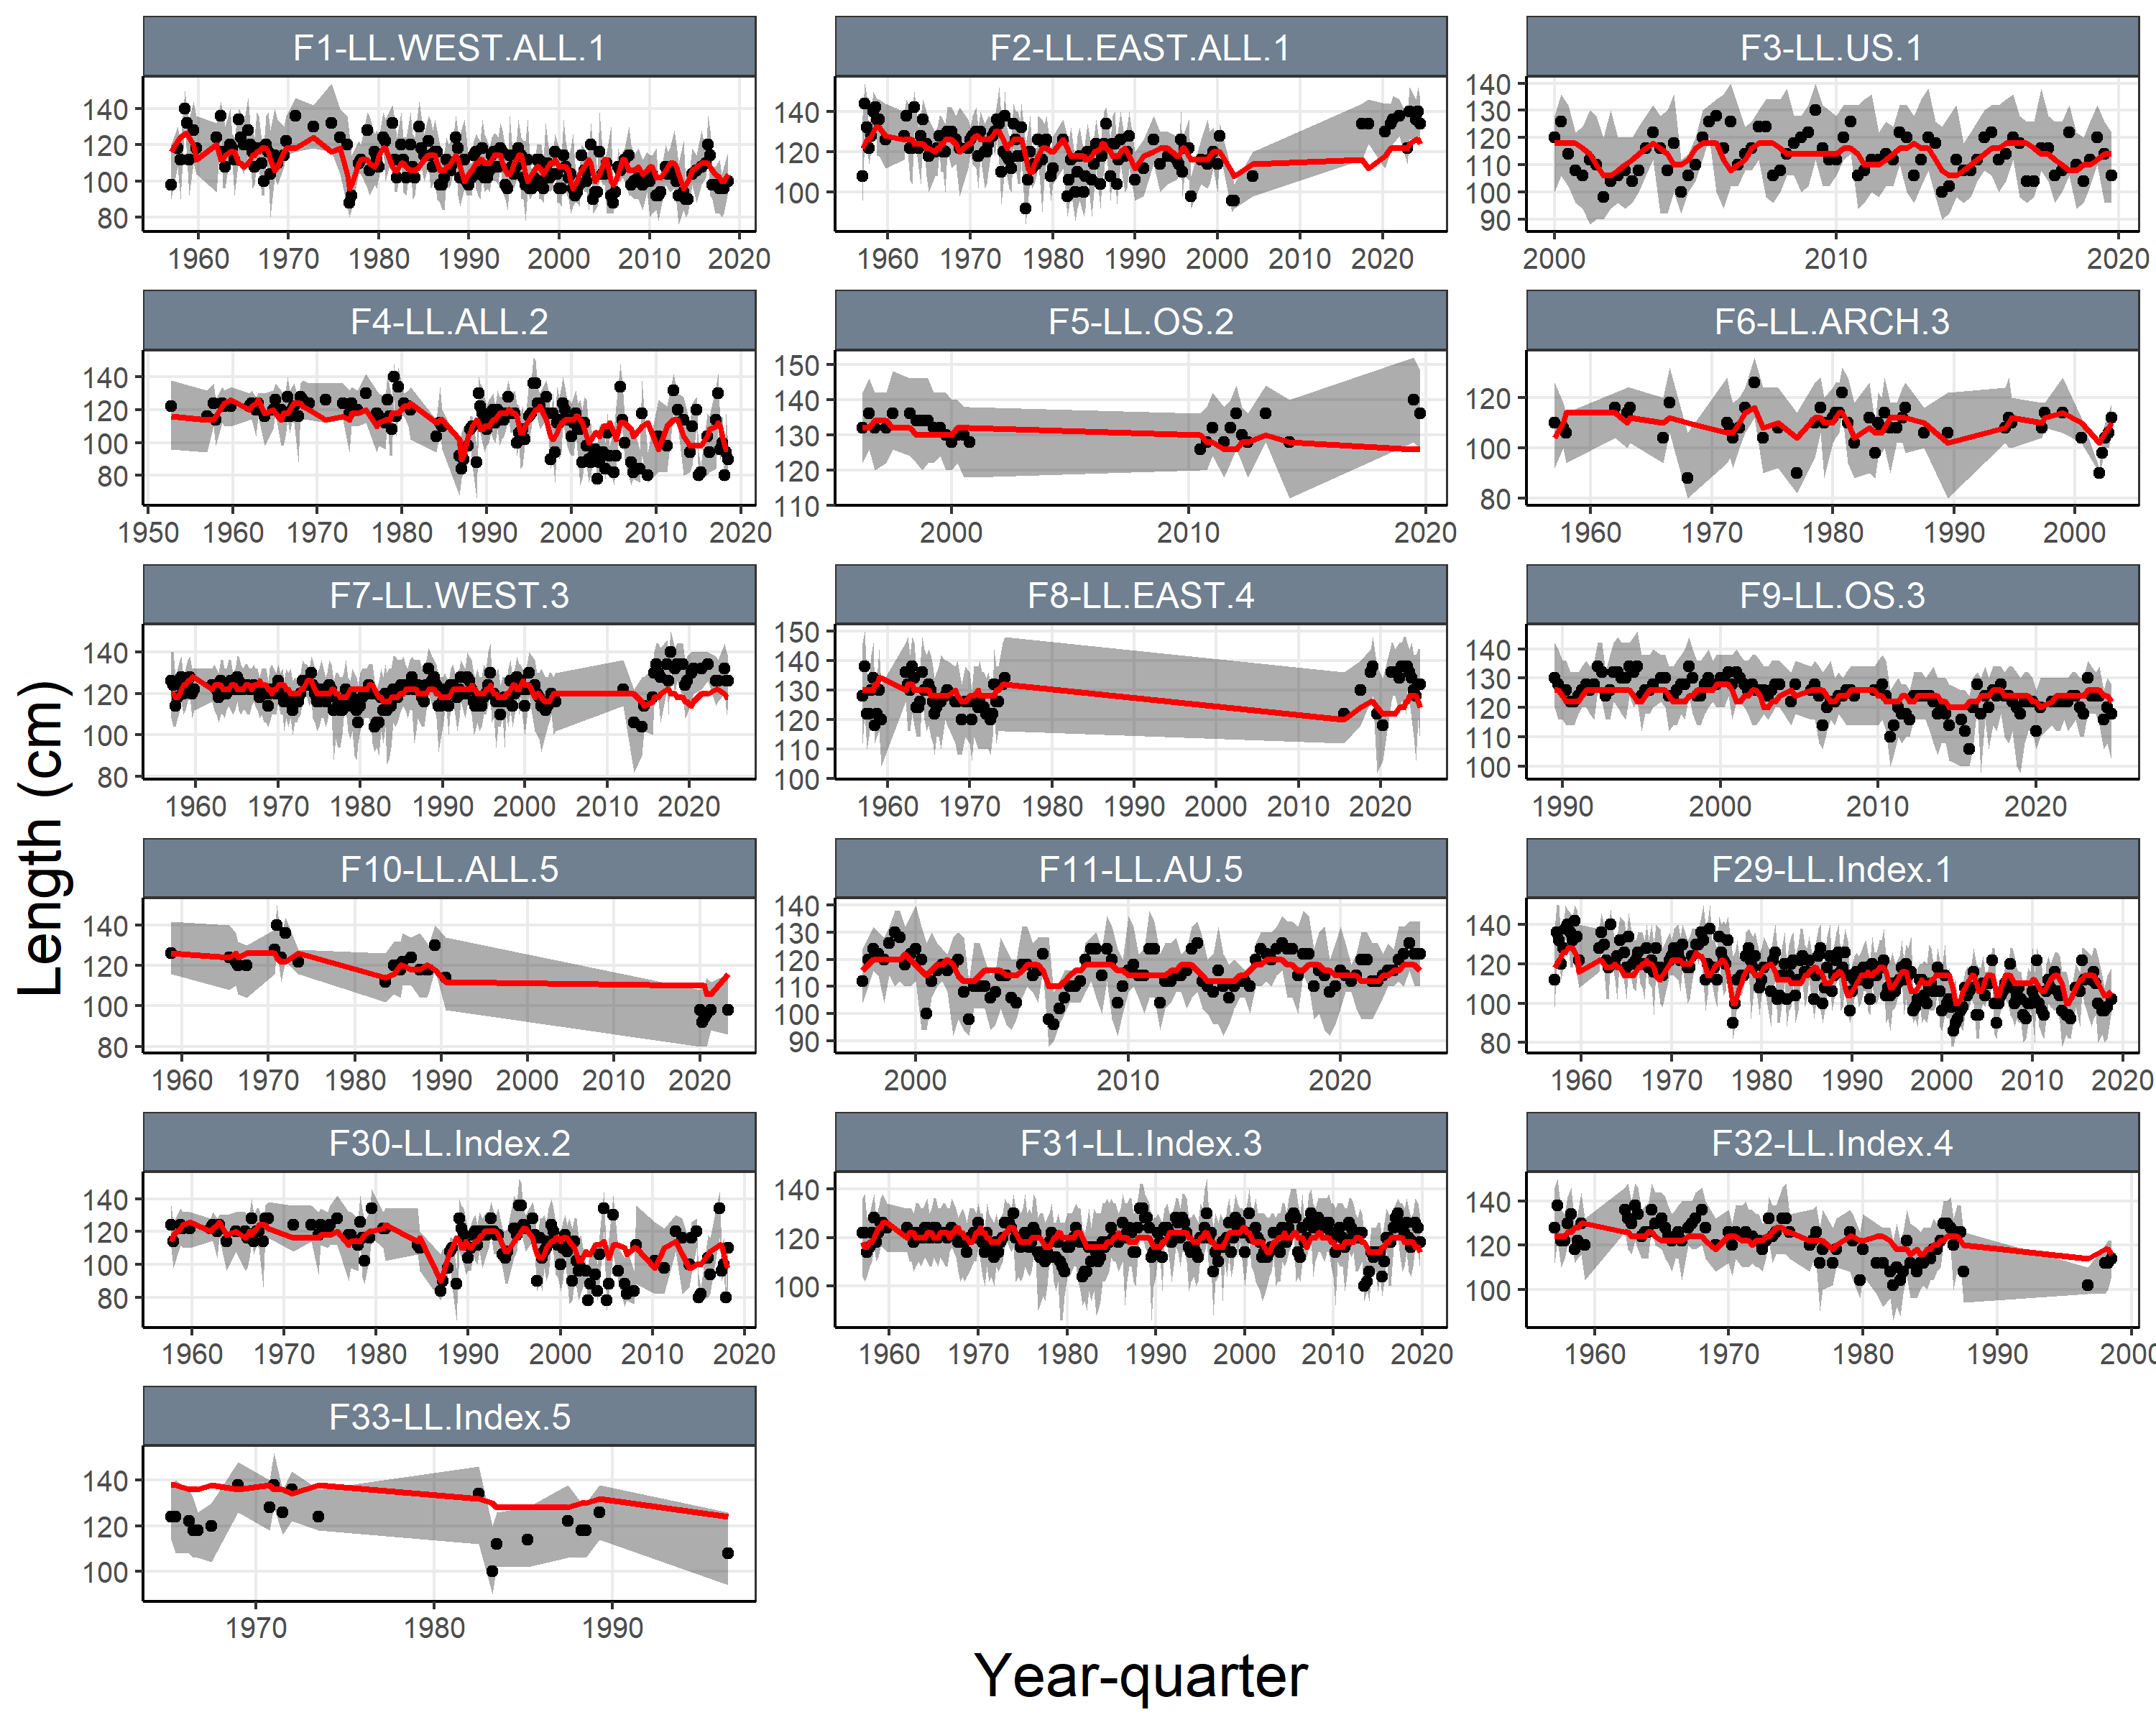
\includegraphics[width=1\linewidth,height=\textheight,keepaspectratio]{figures/length_fit_time_series_ll.png}
%DIFDELCMD <

%DIFDELCMD < }
%DIFDELCMD <

%DIFDELCMD < \caption{\label{fig-length-fit-timeseries-ll}Observed (red points) and
%DIFDELCMD < predicted (red line) median fish lengths (FL, cm) for the longline
%DIFDELCMD < fisheries for the 2026 diagnostic model. The uncertainty intervals (gray
%DIFDELCMD < shading) represent the values encompassed by the 25\% and 75\%
%DIFDELCMD < quantiles. Sampling data are by quarter and only length samples with
%DIFDELCMD < more than 250 fish per quarter/fishery strata are plotted.}
%DIFDELCMD <

%DIFDELCMD < \end{figure}%%%
\DIFdelend \DIFaddbegin \begin{figure}[H]

\centering{

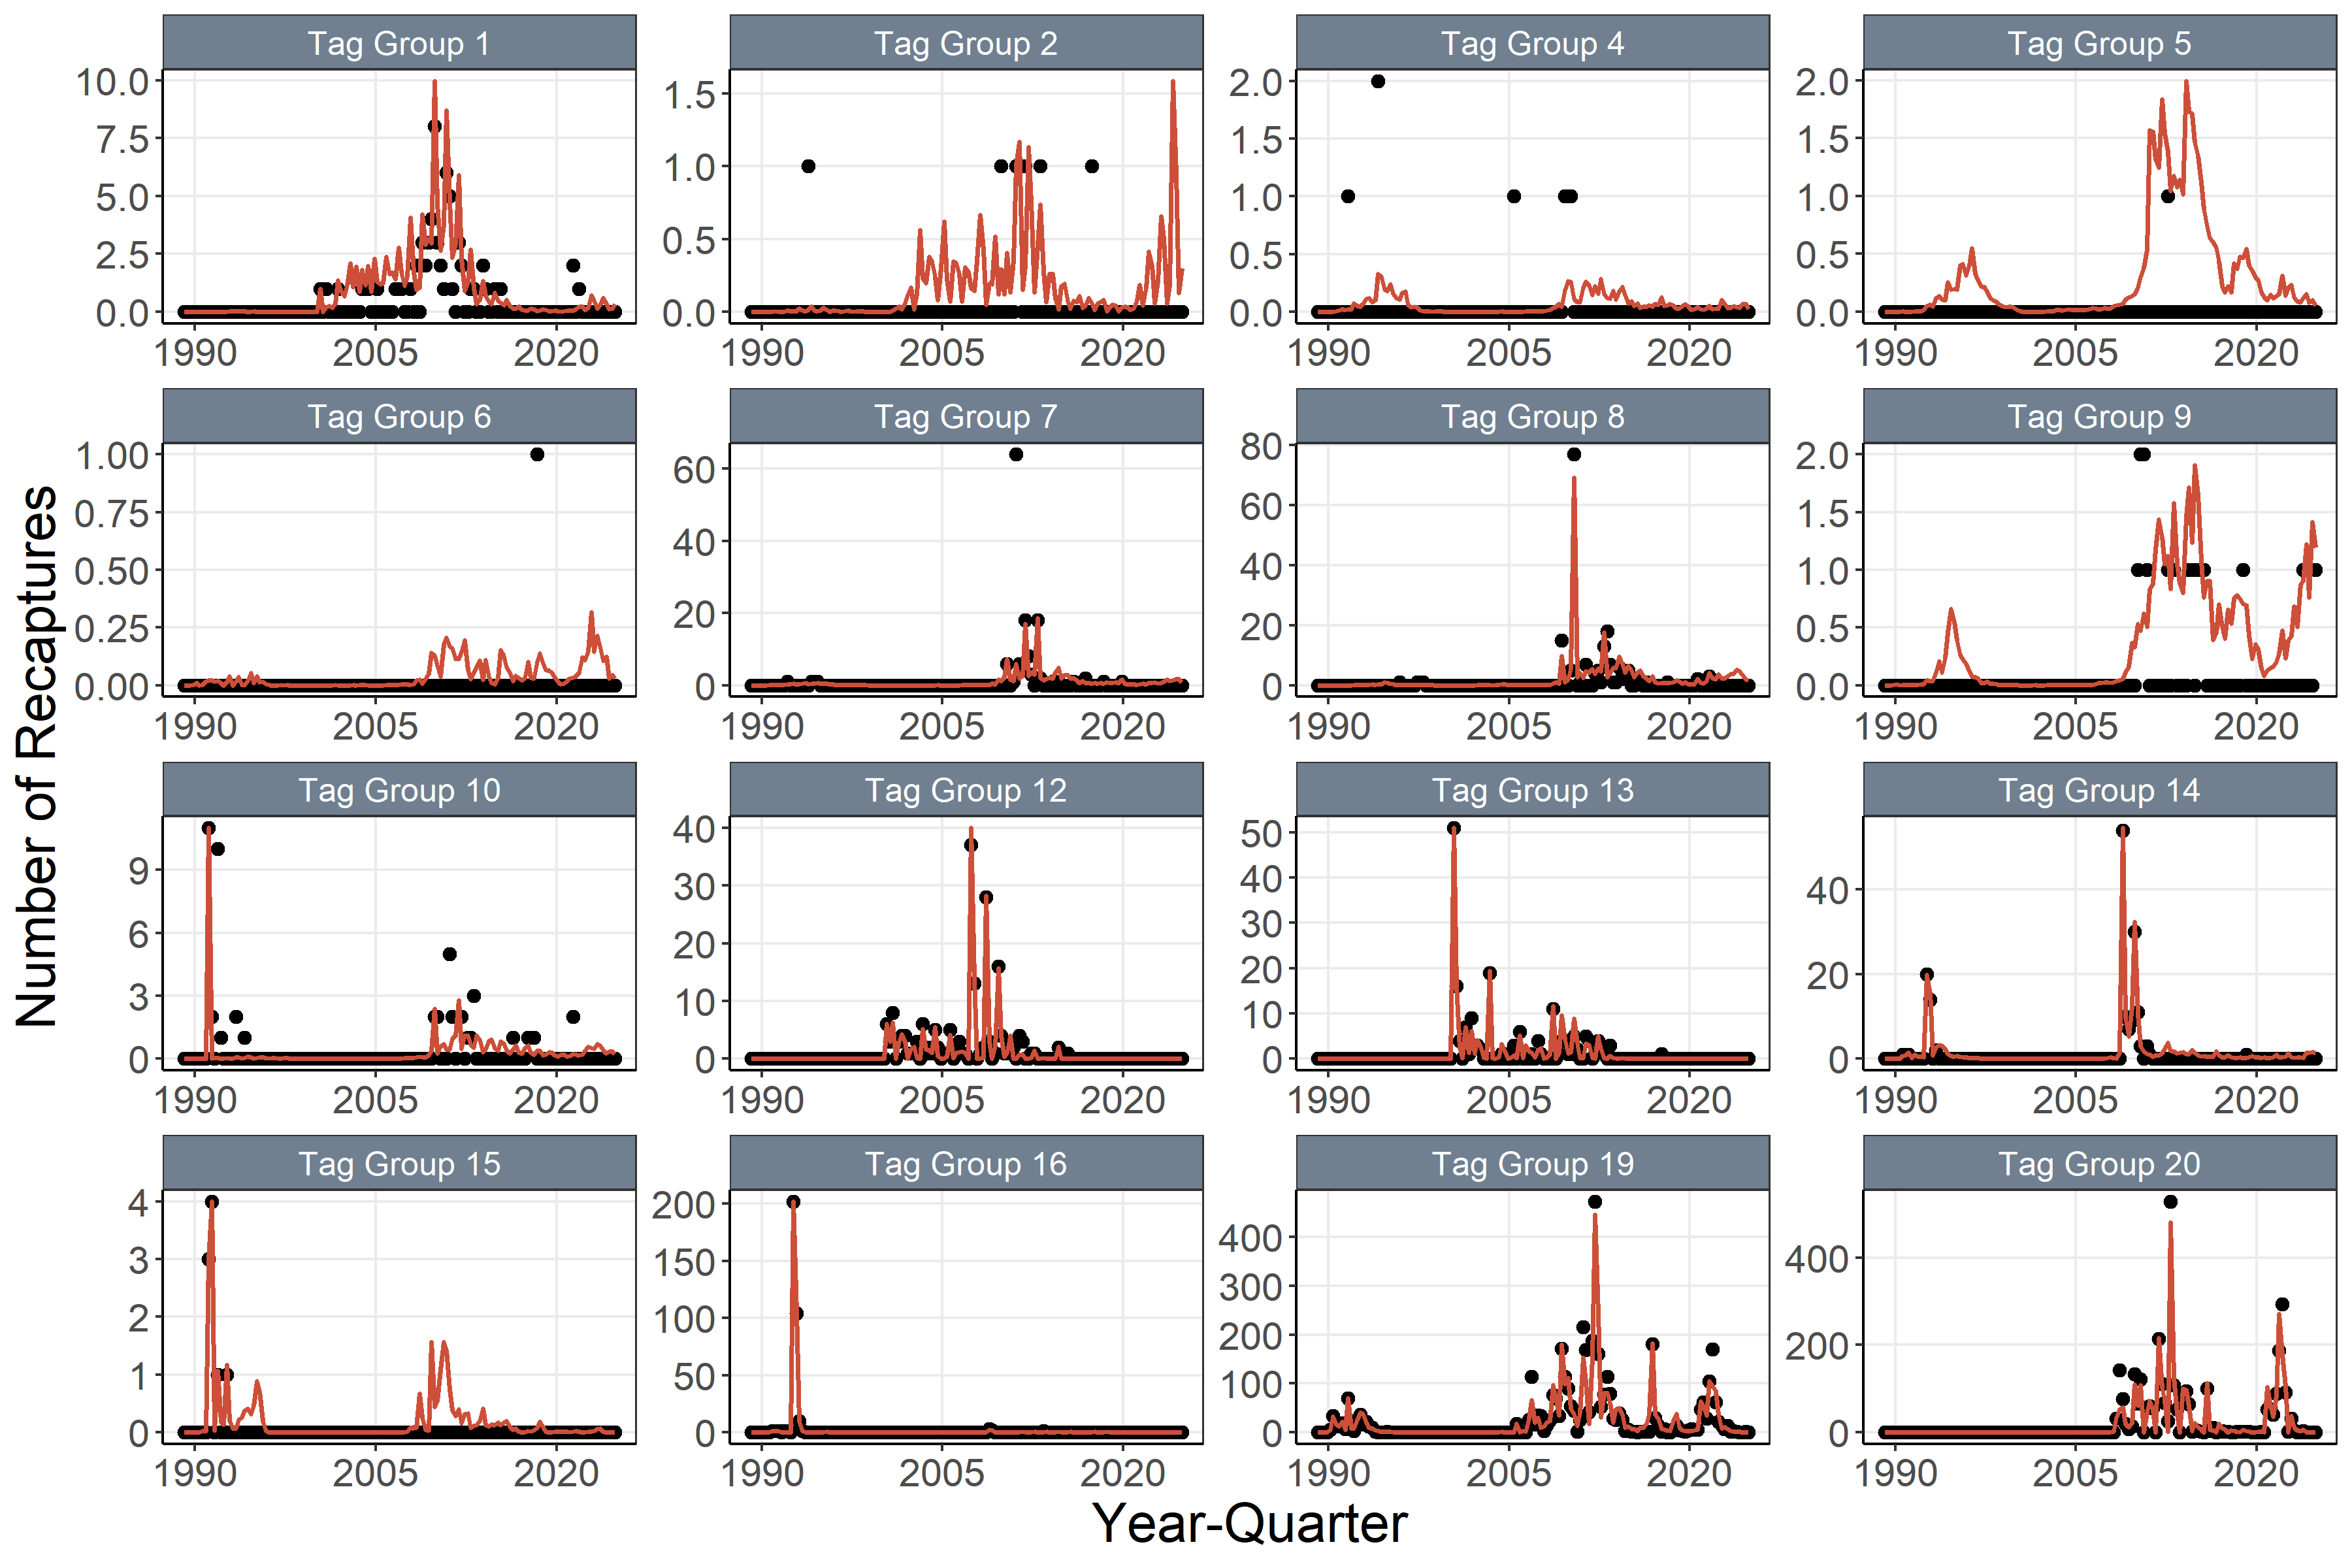
\includegraphics[width=1\linewidth,height=\textheight,keepaspectratio]{figures/tag_recapture_fit_years_groups.png}

}

\caption{\label{fig-tag-recapture-fit-years-groups}Observed (black
points) and model-predicted (red lines) tag recaptures through time for
the principal tag-recapture groups in the 2026 diagnostic model.}

\end{figure}\DIFaddend %

\DIFdelbegin %DIFDELCMD < \begin{figure}[H]
%DIFDELCMD <

%DIFDELCMD < \centering{
%DIFDELCMD <

%DIFDELCMD < 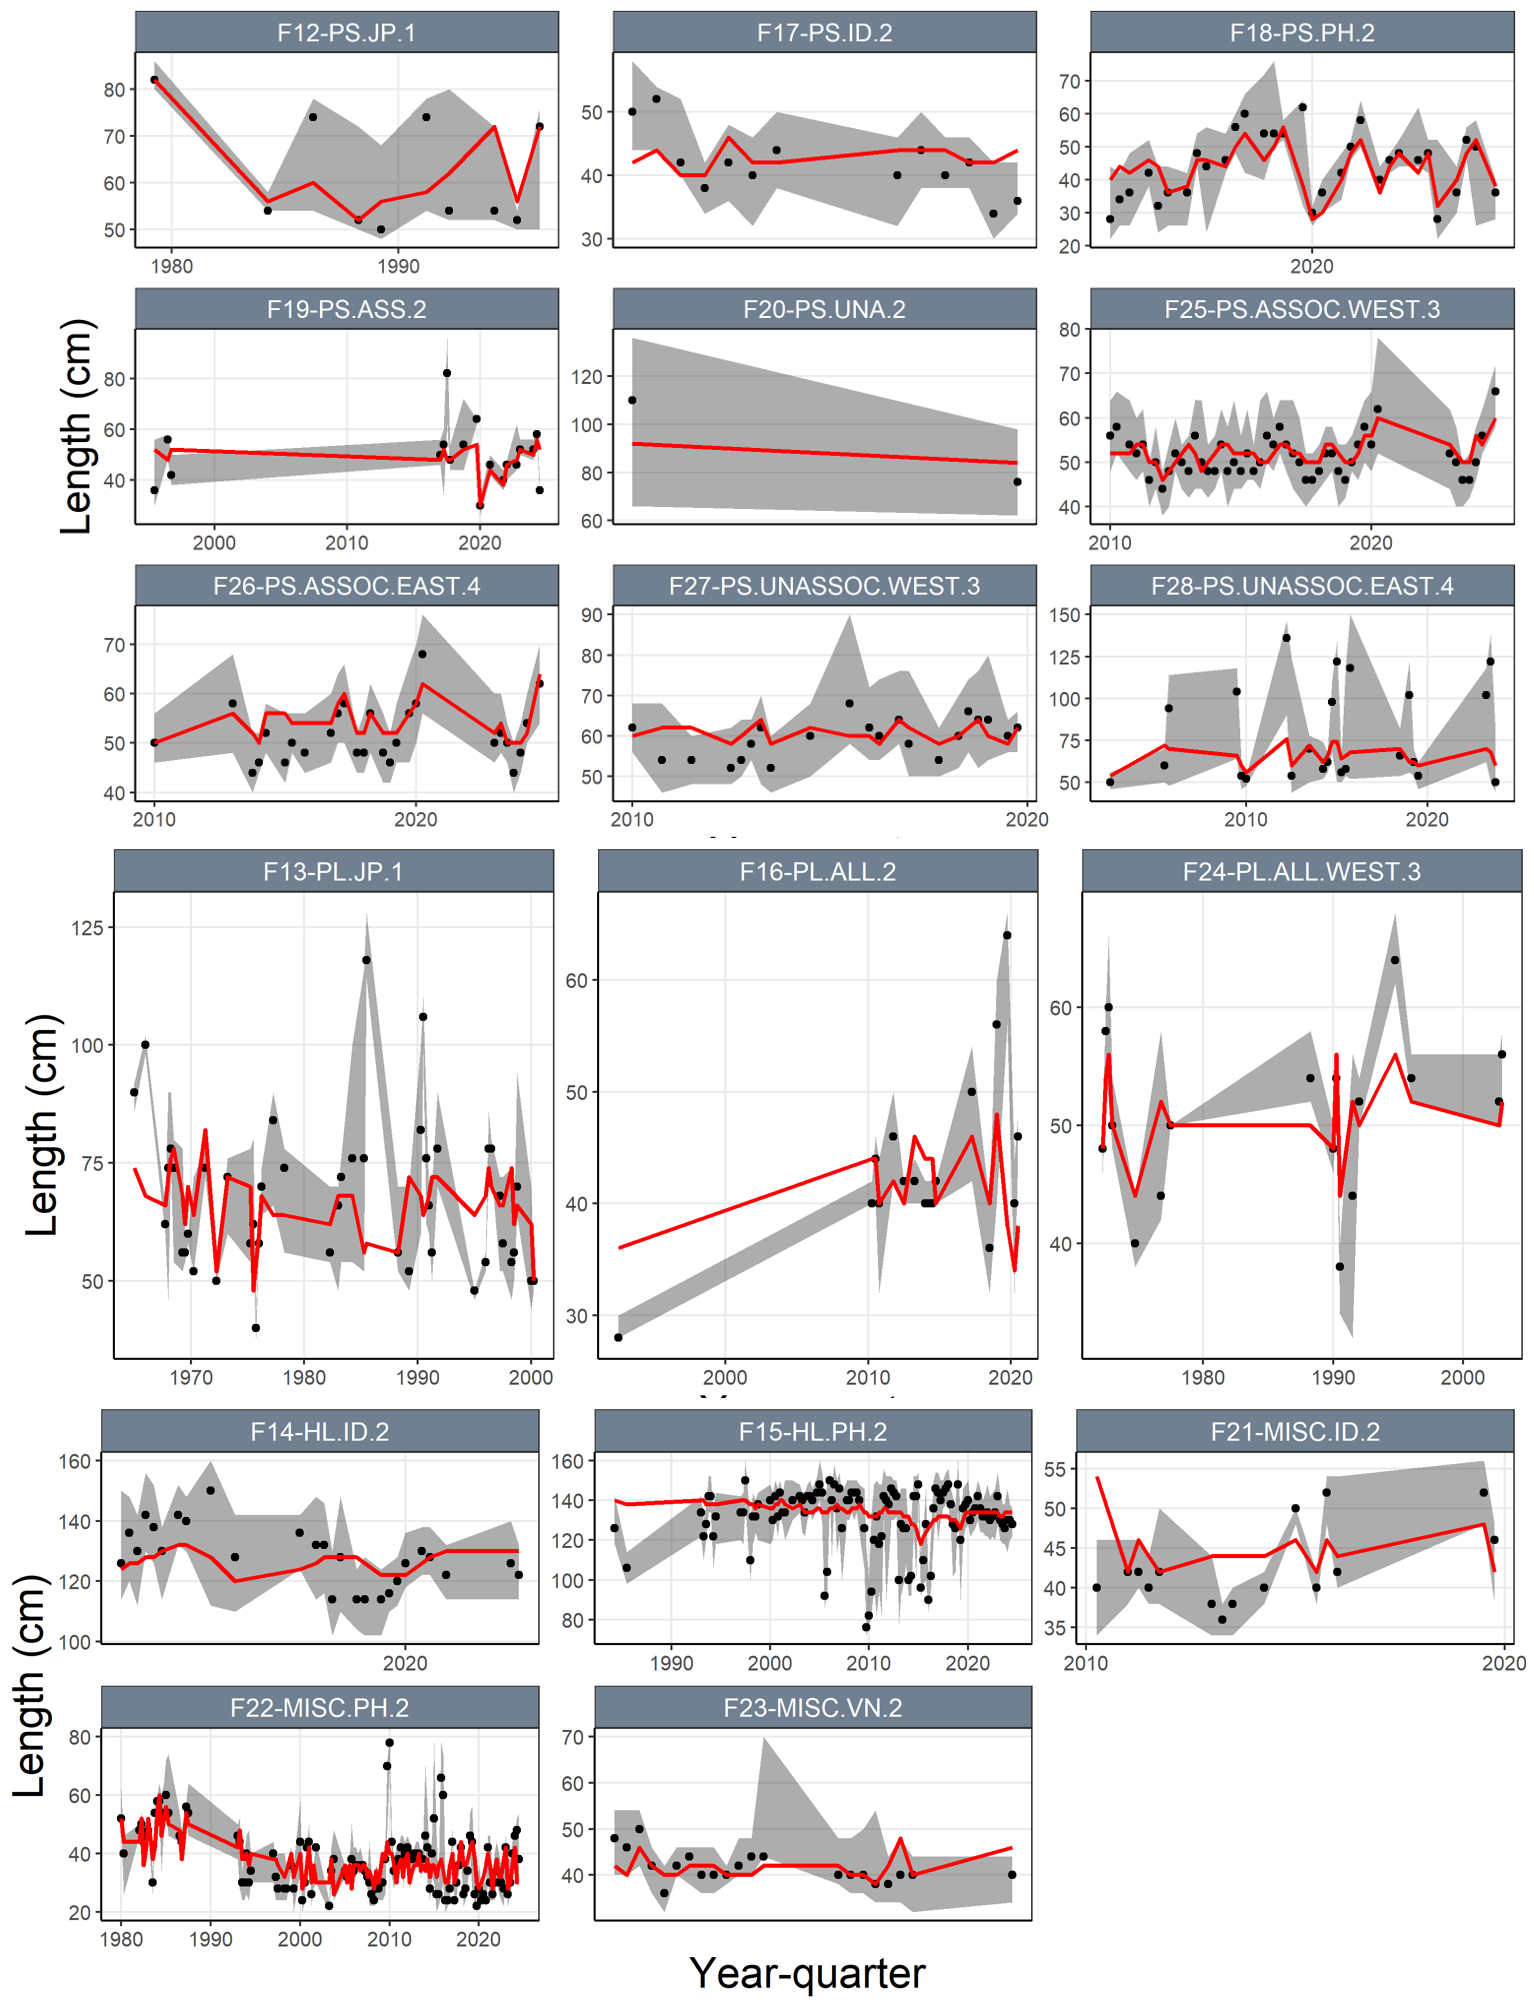
\includegraphics[width=0.75\linewidth,height=\textheight,keepaspectratio]{figures/length_fit_time_series_other.png}
%DIFDELCMD <

%DIFDELCMD < }
%DIFDELCMD <

%DIFDELCMD < \caption{\label{fig-length-fit-timeseries-other}Observed (red points)
%DIFDELCMD < and predicted (red line) median fish lengths (FL, cm) for the other
%DIFDELCMD < fisheries for the 2026 diagnostic model. The uncertainty intervals (gray
%DIFDELCMD < shading) represent the values encompassed by the 25\% and 75\%
%DIFDELCMD < quantiles. Sampling data are by quarter and only length samples with
%DIFDELCMD < more than 100 fish per quarter/fishery strata are plotted.}
%DIFDELCMD <

%DIFDELCMD < \end{figure}%%%
\DIFdelend \DIFaddbegin \begin{figure}[H]

\centering{

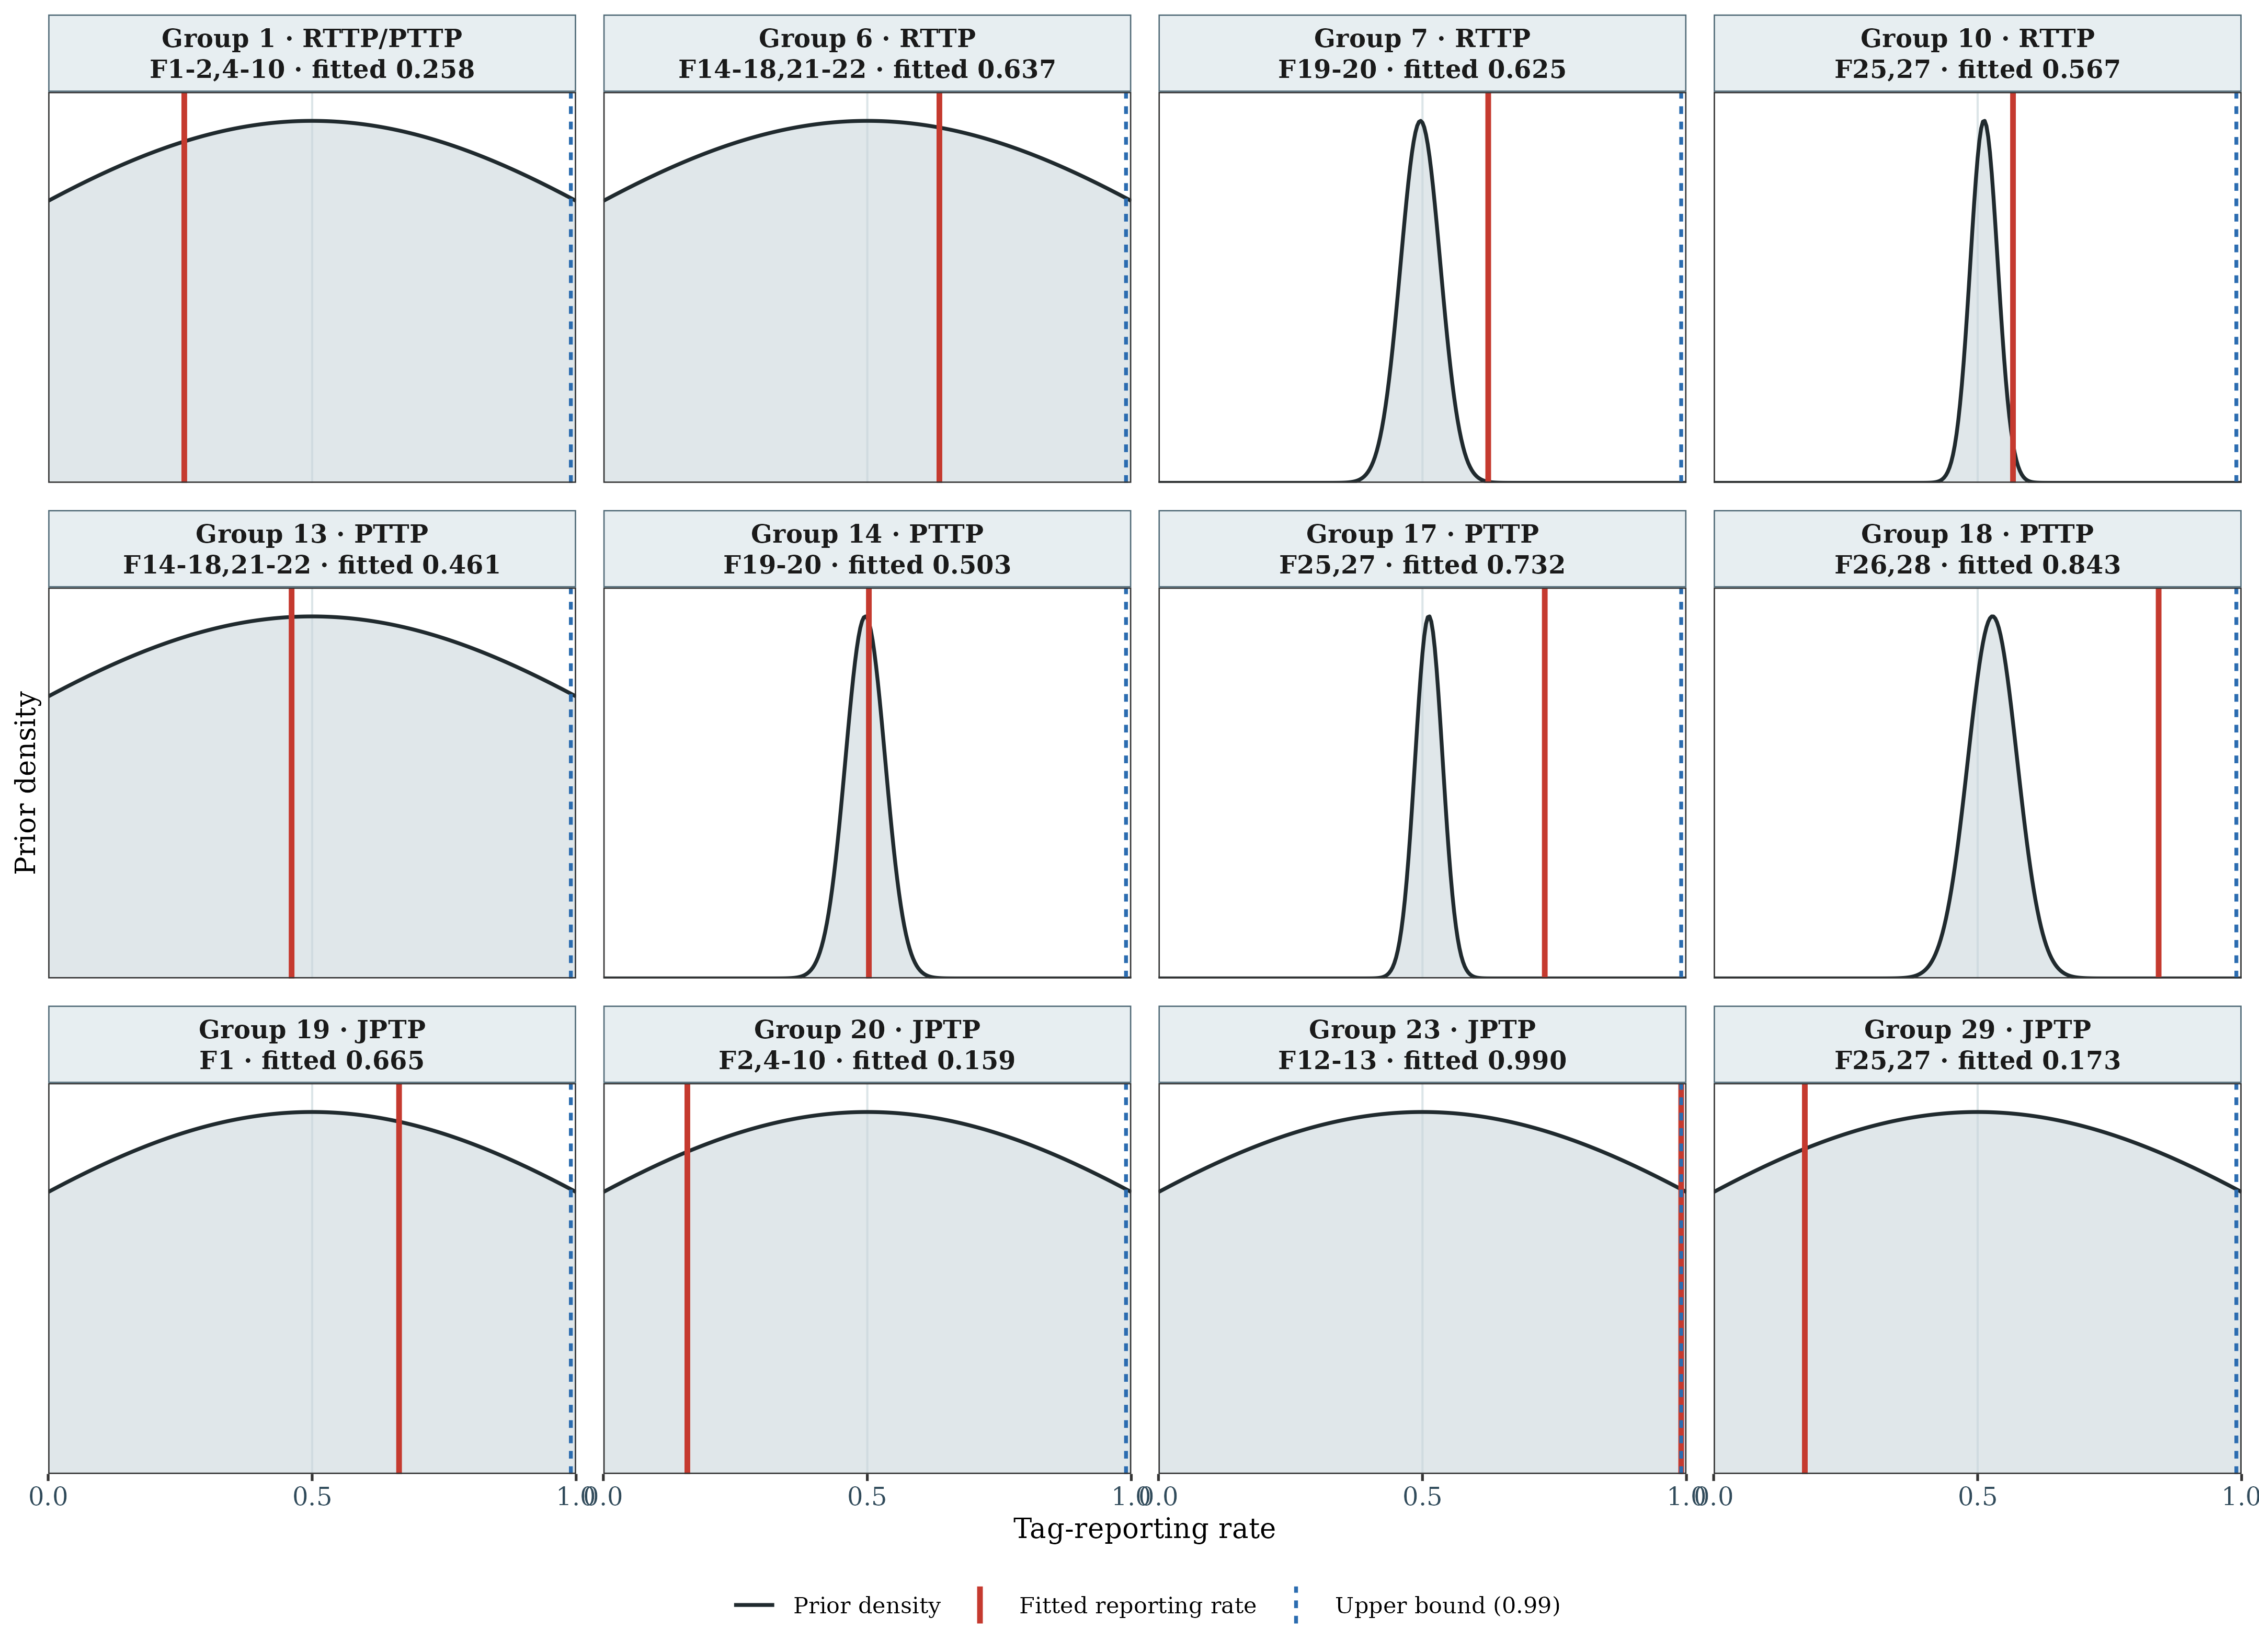
\includegraphics[width=1\linewidth,height=\textheight,keepaspectratio]{figures_new/tag-reporting-rates-active.png}

}

\caption{\label{fig-tag-reporting-rates-active}\label{fig-tag-report-rates-rttp-pttp}\label{fig-tag-report-rates-jtpt}Fitted tag-reporting
rates for the 12 groups estimated in the diagnostic model. Panels
identify the MFCL reporting-rate group, tagging programme and recapture
fisheries. Black curves show the prior density, red vertical lines show
fitted reporting rates and blue dashed lines mark the 0.99 upper bound.
Group 23 reached the upper bound. Fixed groups and the inactive Group 31
placeholder assigned to Index fisheries F29--F33 are not shown. Open the
\href{https://pacificcommunity.github.io/ofp-sam-bet-2026-diagnostic/bet-2026-diagnostic-report.html}{interactive
diagnostic report}.}

\end{figure}\DIFaddend %

\DIFdelbegin %DIFDELCMD < \begin{figure}[H]
%DIFDELCMD <

%DIFDELCMD < \centering{
%DIFDELCMD <

%DIFDELCMD < 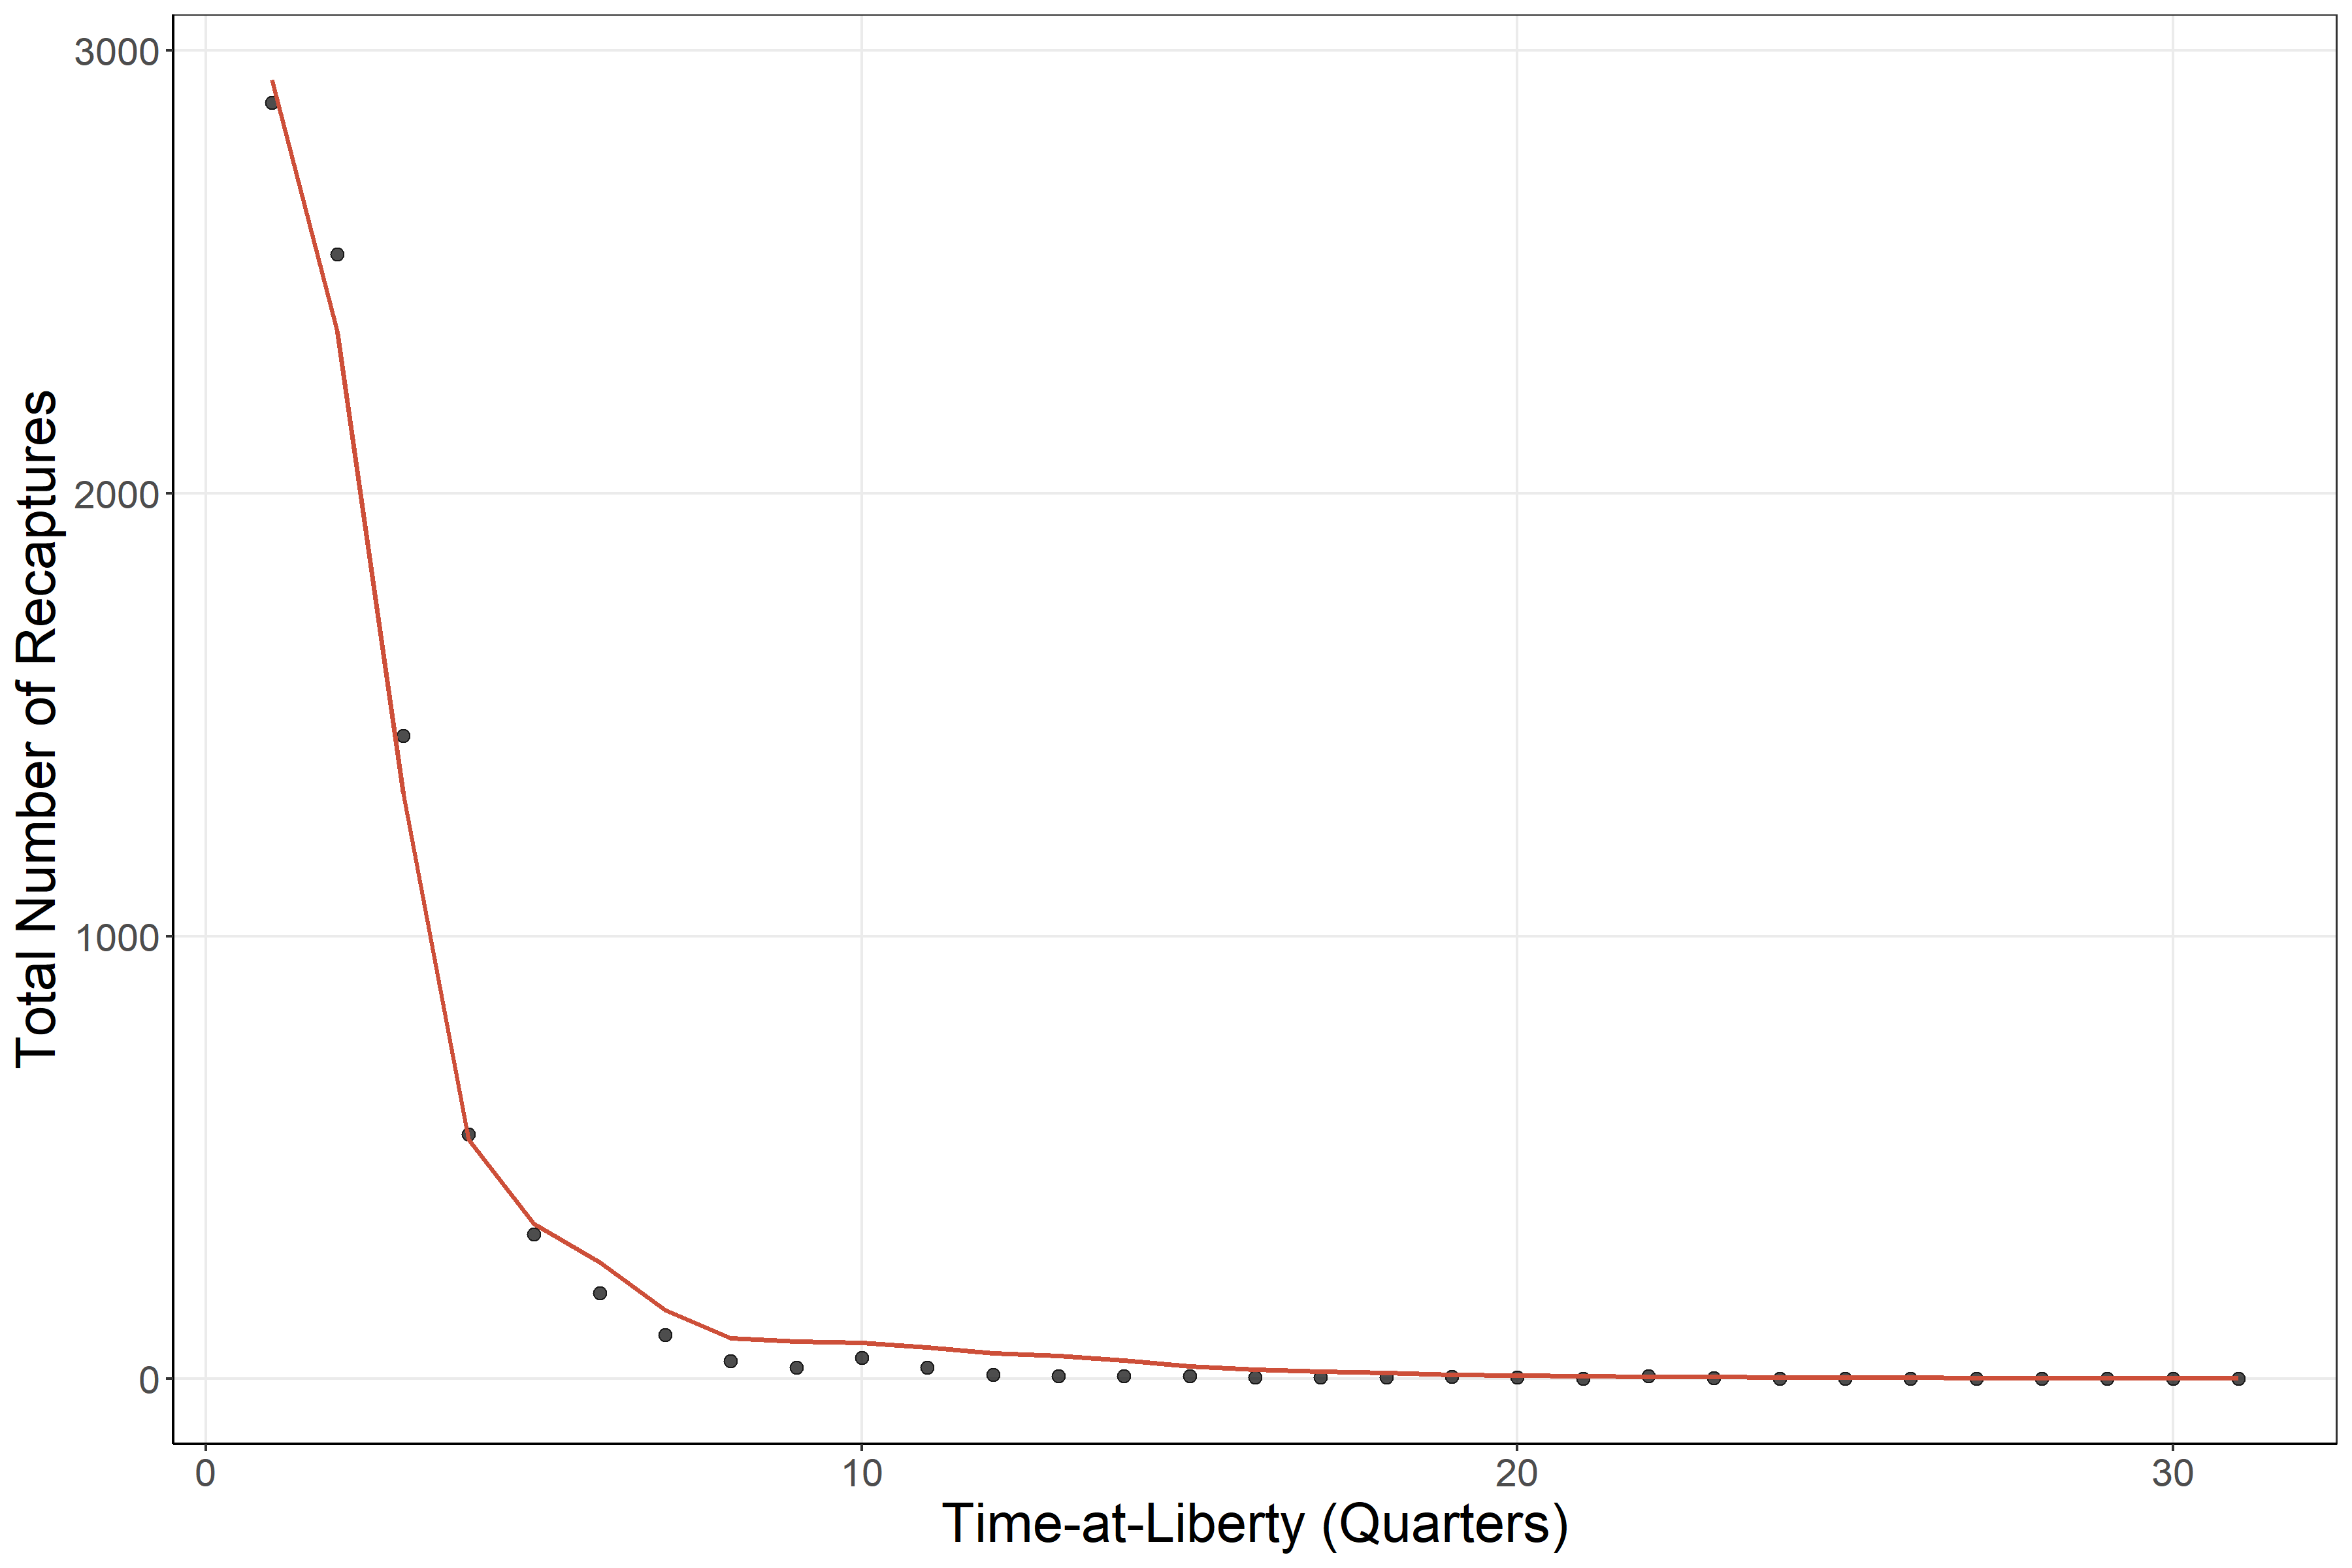
\includegraphics[width=1\linewidth,height=\textheight,keepaspectratio]{figures/tag_attrition_all.png}
%DIFDELCMD <

%DIFDELCMD < }
%DIFDELCMD <

%DIFDELCMD < \caption{\label{fig-tag-attrition-all}Observed (black points) and
%DIFDELCMD < model-predicted (red line) tag attrition across all tag release events
%DIFDELCMD < for the 2026 diagnostic model.}
%DIFDELCMD <

%DIFDELCMD < \end{figure}%%%
\DIFdelend \DIFaddbegin \begin{figure}[H]

\centering{

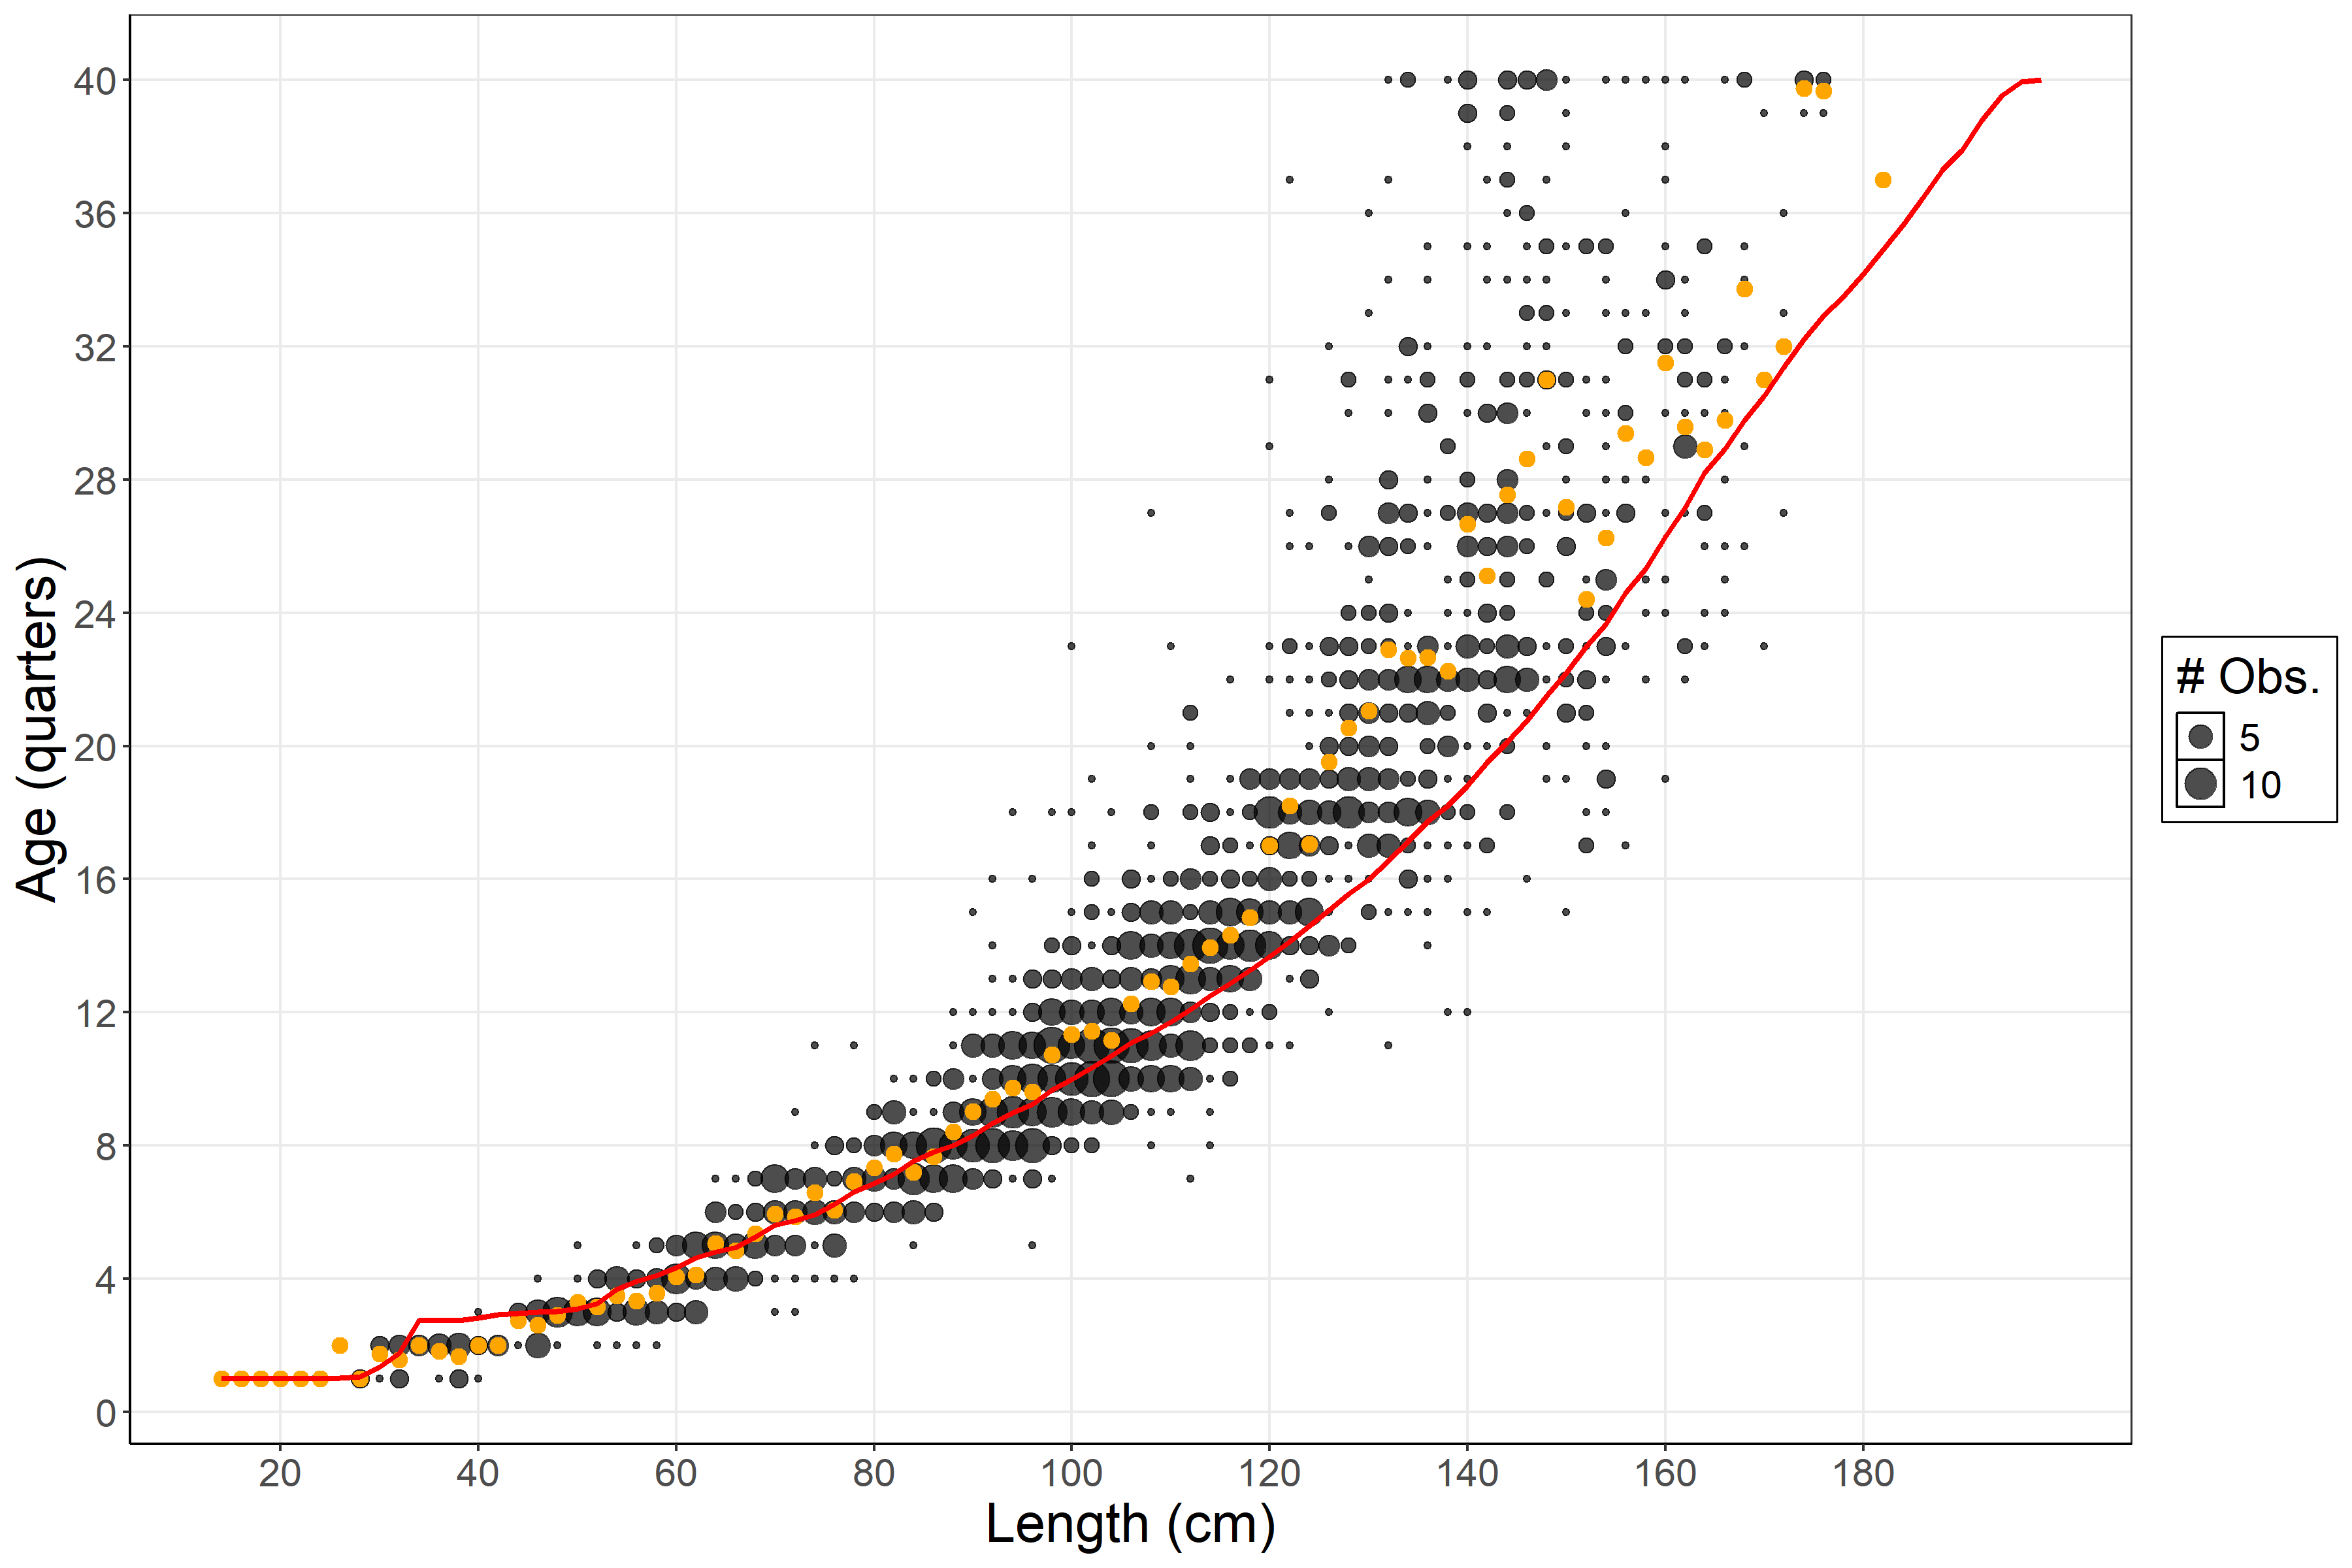
\includegraphics[width=0.85\linewidth,height=\textheight,keepaspectratio]{figures/caal_aggregate_fits.png}

}

\caption{\label{fig-caal-fits}Model-estimated mean age at length (line)
and observed conditional ages (circles), pooled across all samples. The
vertical distribution of points shows the observed age distribution at
each length.}

\end{figure}\DIFaddend %

\DIFdelbegin %DIFDELCMD < \begin{figure}[H]
%DIFDELCMD <

%DIFDELCMD < \centering{
%DIFDELCMD <

%DIFDELCMD < 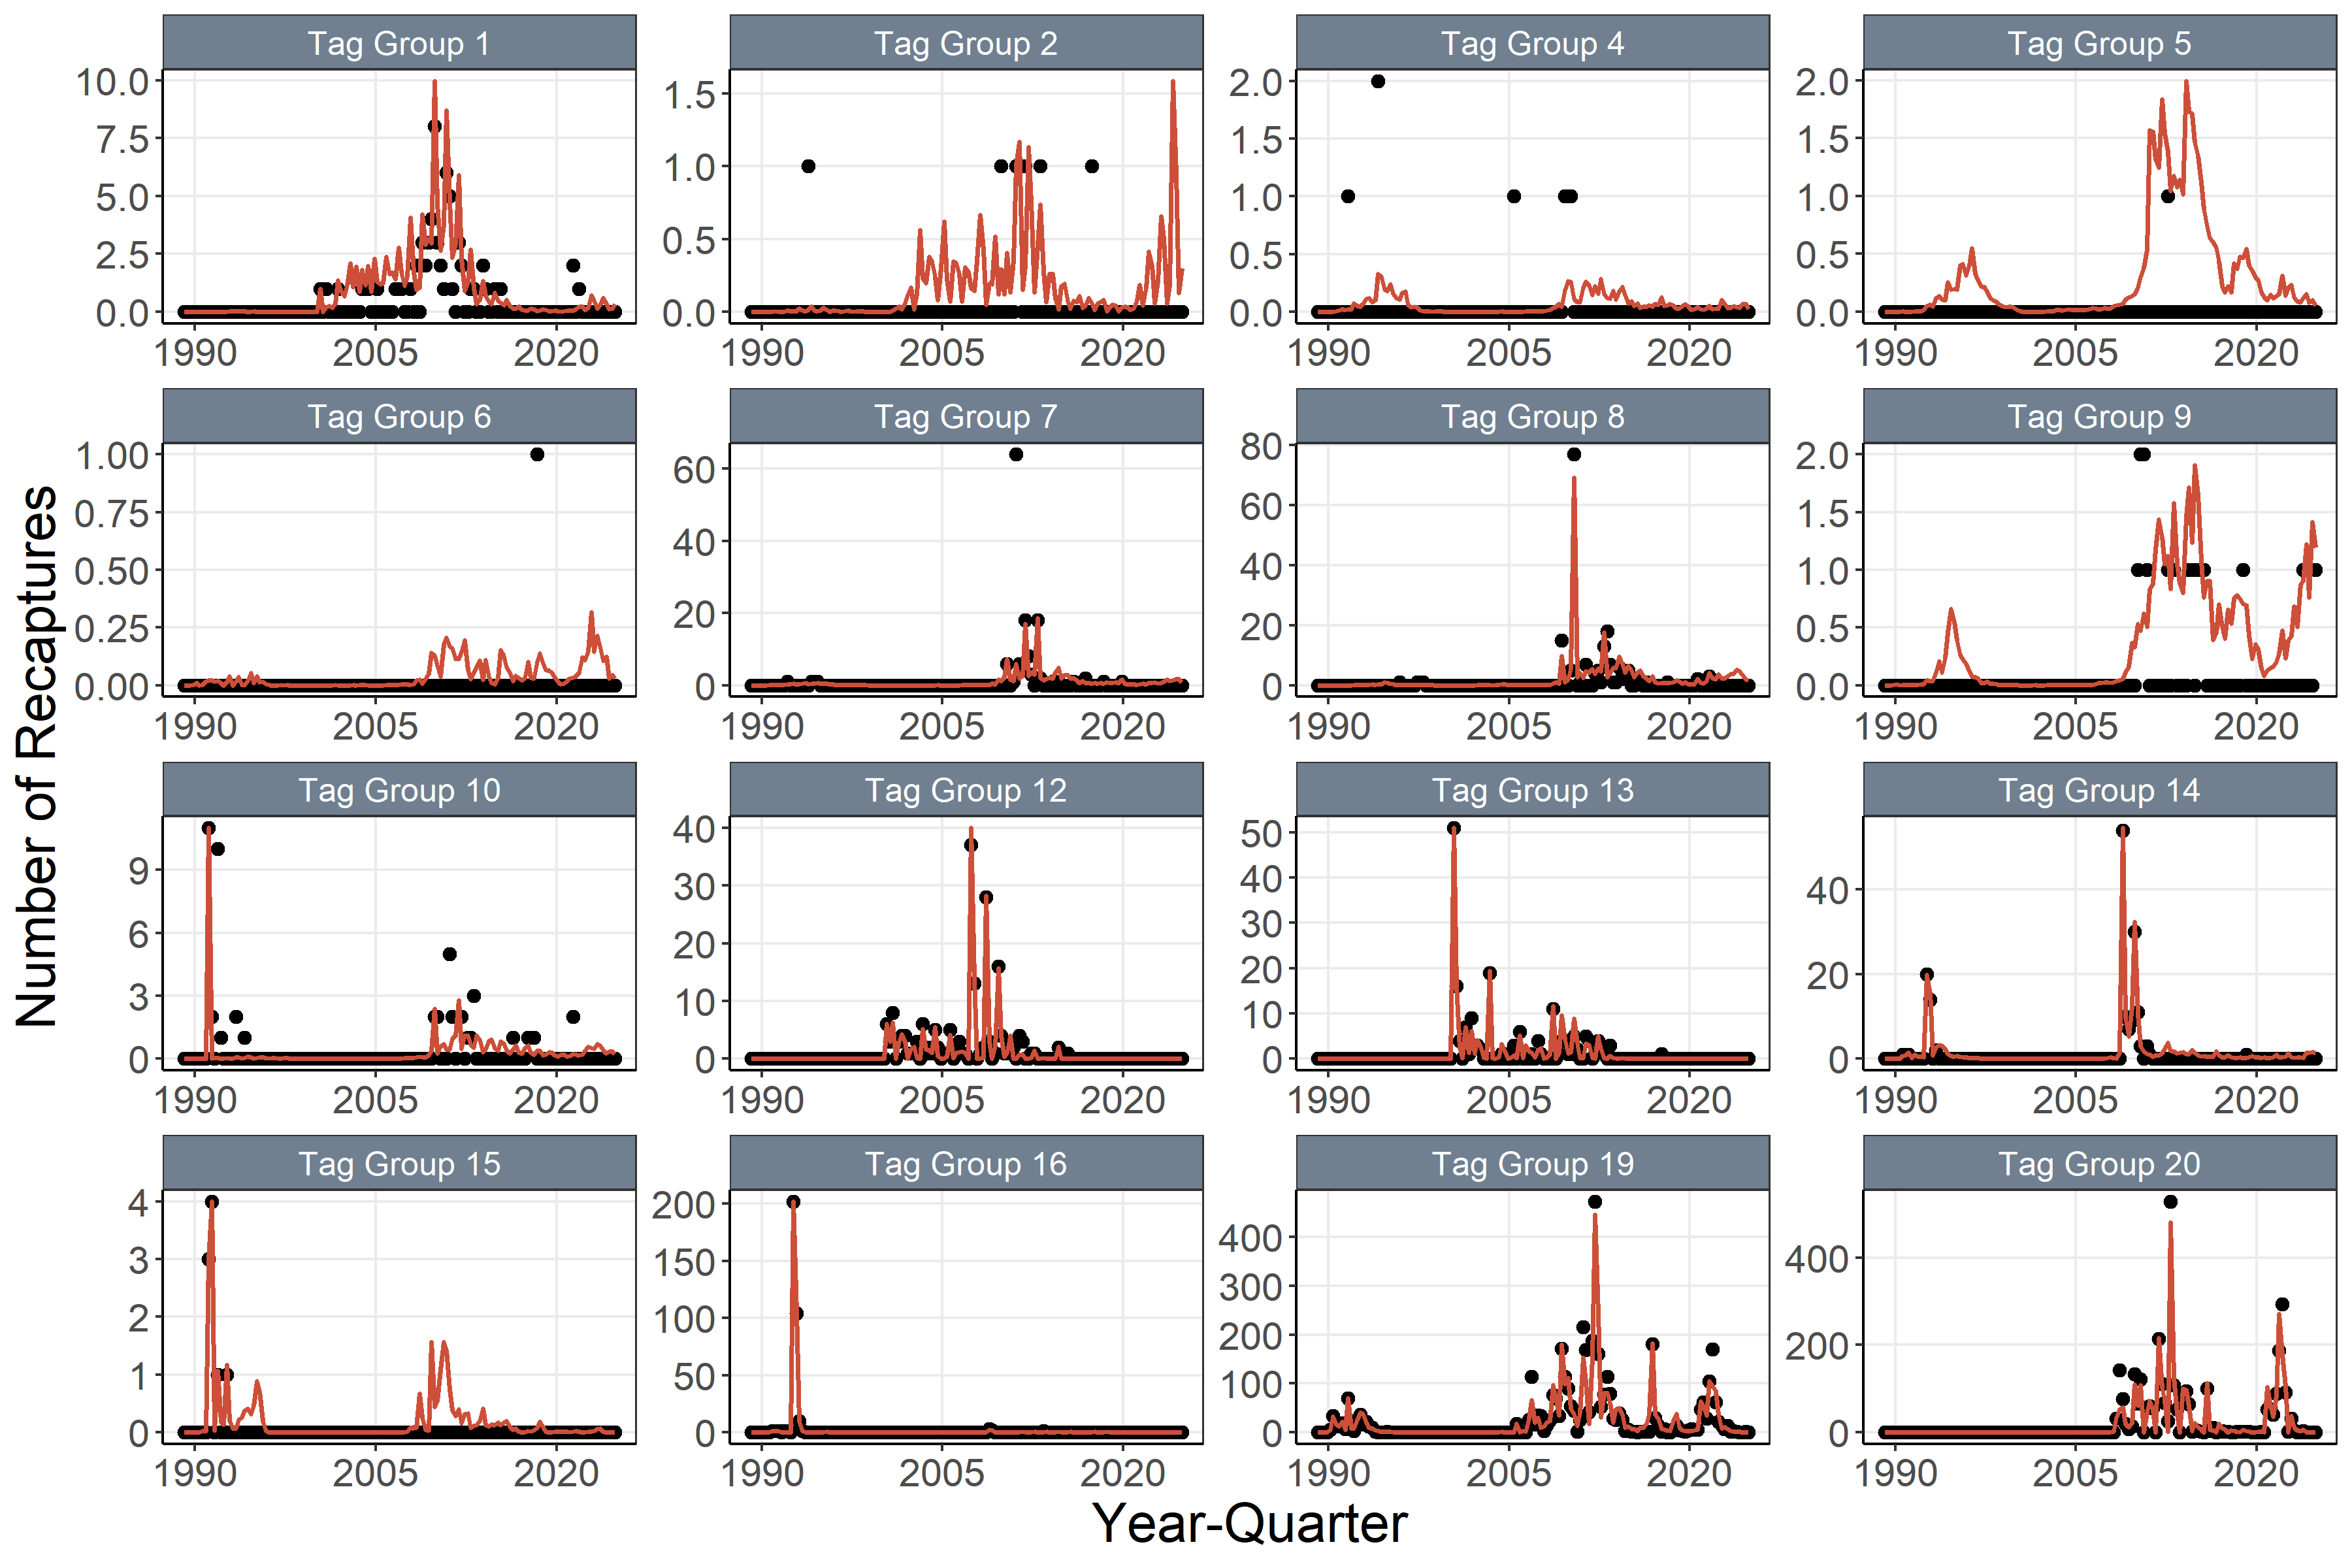
\includegraphics[width=1\linewidth,height=\textheight,keepaspectratio]{figures/tag_recapture_fit_years_groups.png}
%DIFDELCMD <

%DIFDELCMD < }
%DIFDELCMD <

%DIFDELCMD < \caption{\label{fig-tag-recapture-fit-years-groups}Observed (black
%DIFDELCMD < points) and model-predicted (red lines) tag attrition by tagging
%DIFDELCMD < programme for the 2026 diagnostic model.}
%DIFDELCMD <

%DIFDELCMD < \end{figure}%%%
\DIFdelend \DIFaddbegin \begin{figure}[H]

\centering{

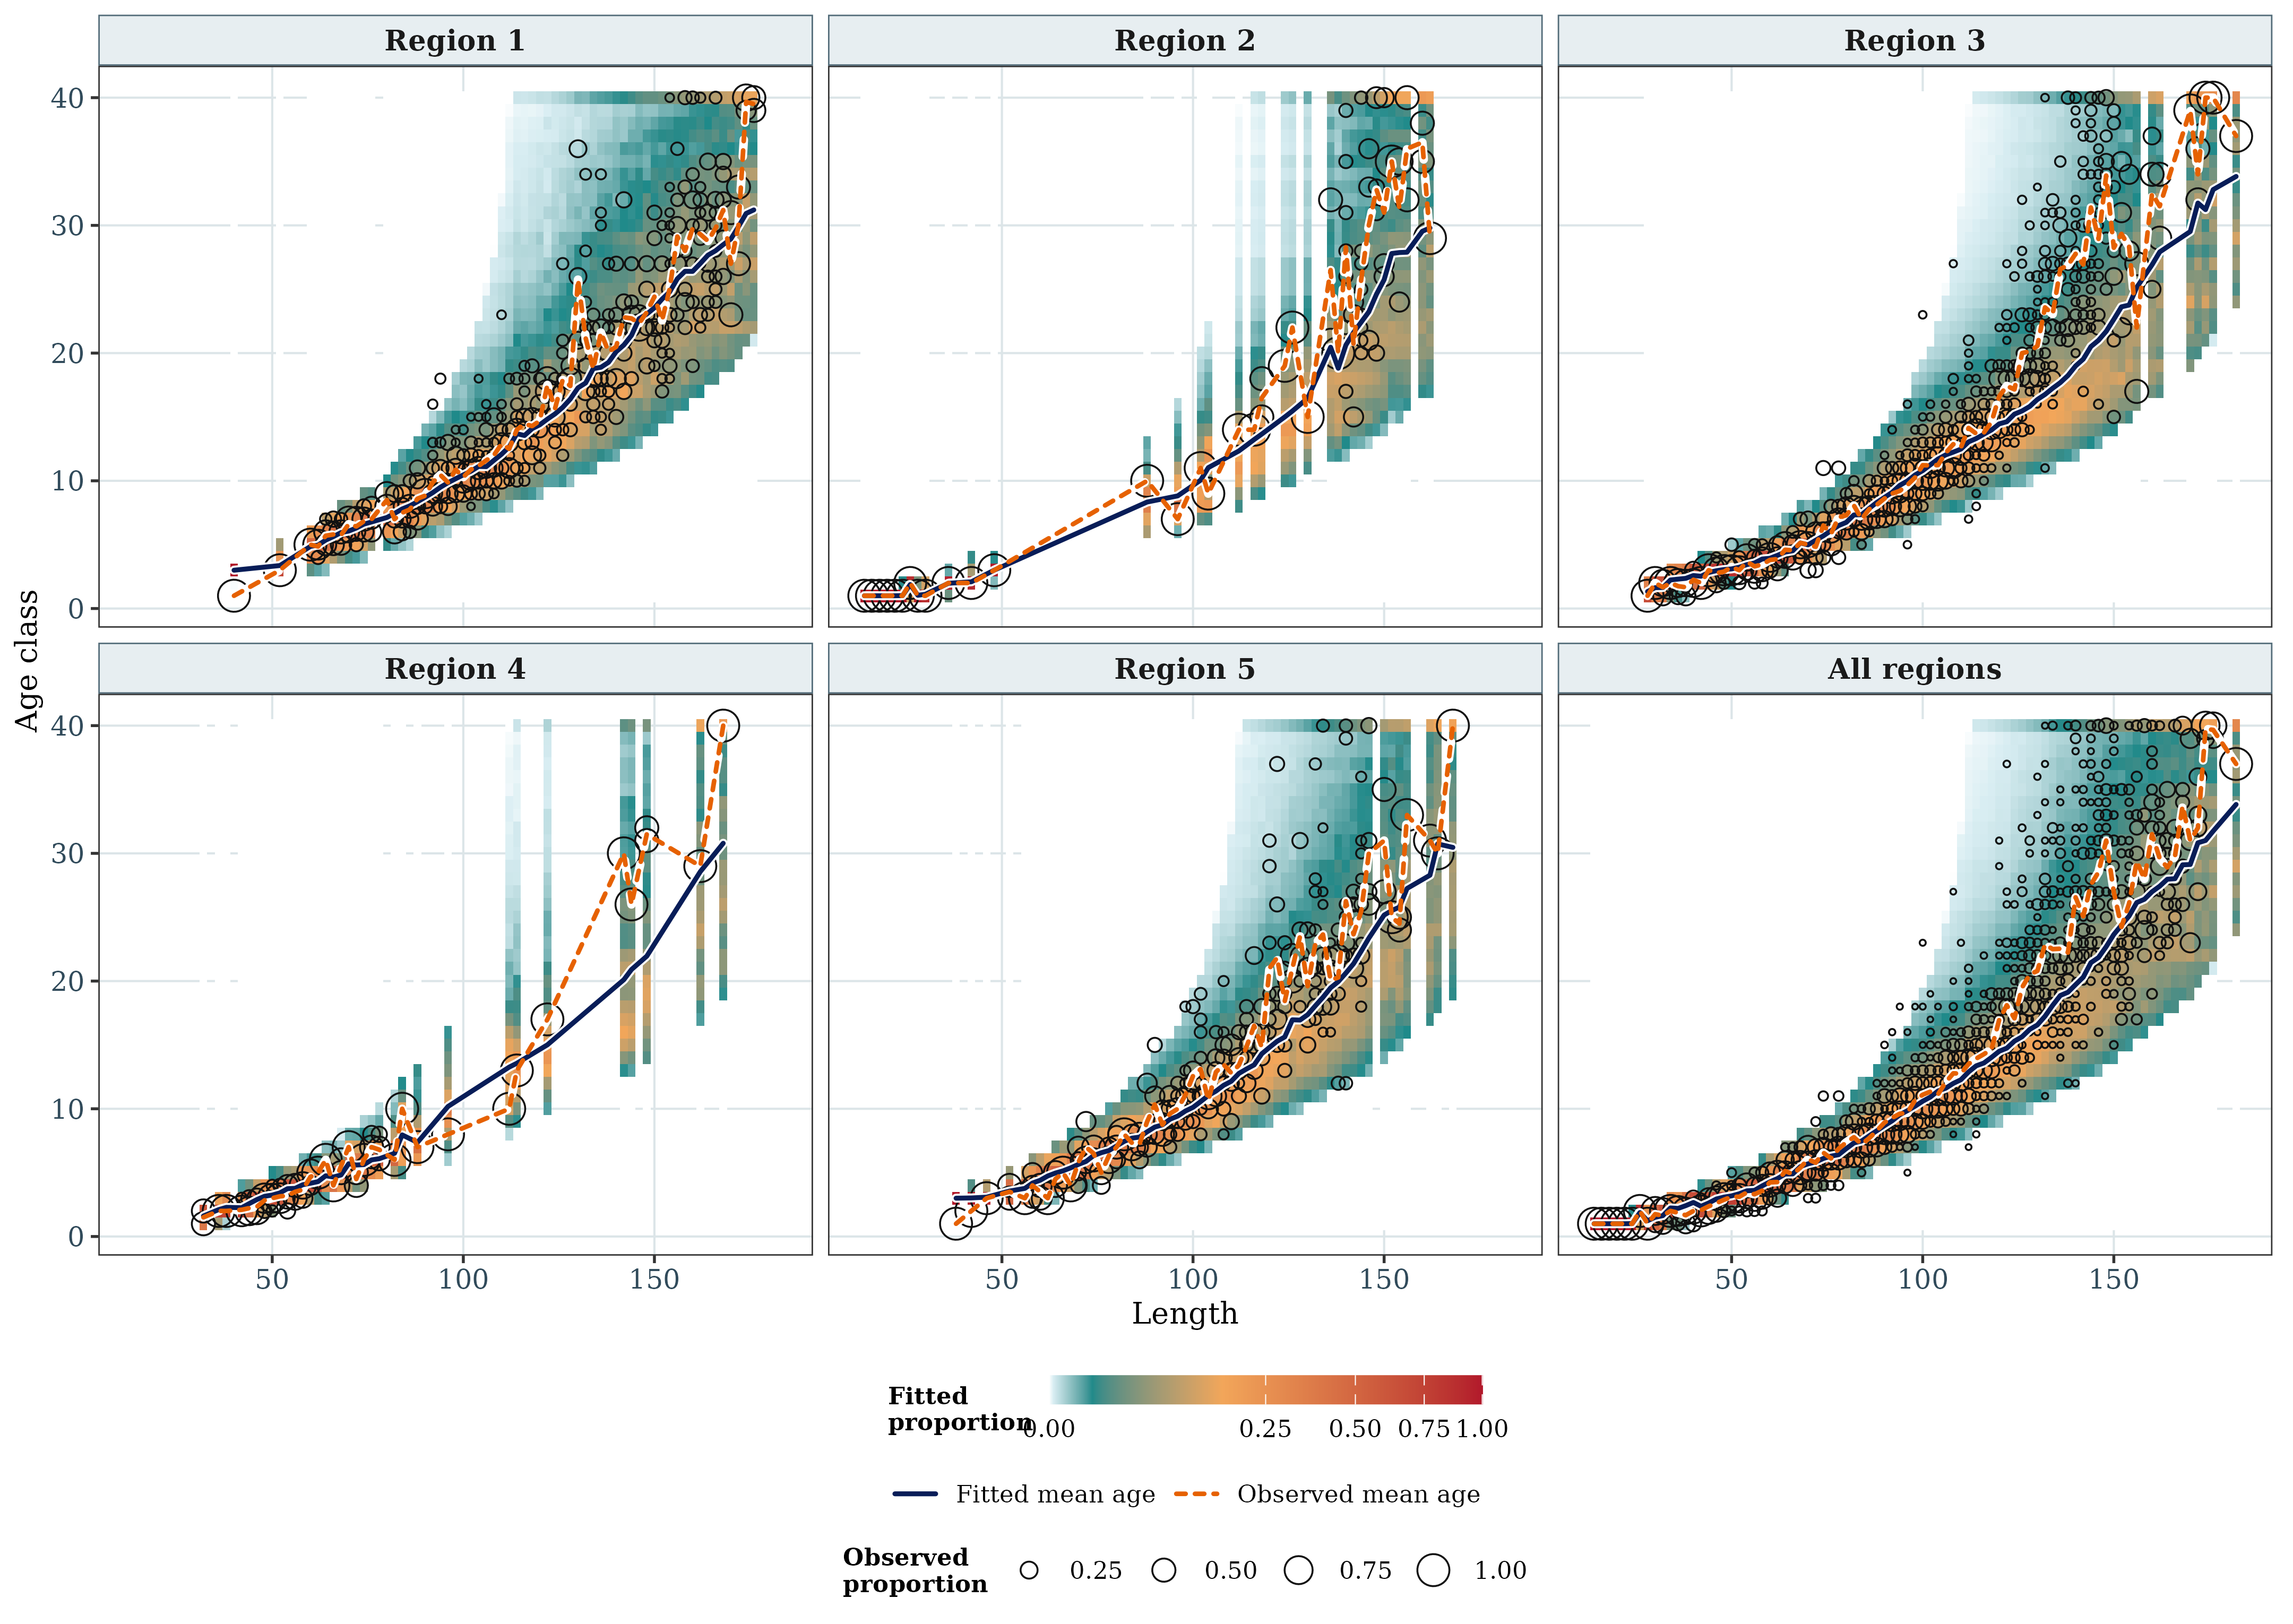
\includegraphics[width=1\linewidth,height=\textheight,keepaspectratio]{figures_new/age-data-fit-by-region.png}

}

\caption{\label{fig-caal-fits-regions}Observed and fitted conditional
age-at-length distributions for the five model regions and the pooled
All regions panel (last). Cells and point sizes show fitted and observed
proportions; solid and dashed lines show their corresponding mean ages
at length. Open the
\href{https://pacificcommunity.github.io/ofp-sam-bet-2026-diagnostic/bet-2026-diagnostic-report.html}{interactive
diagnostic report} for fishery-level detail.}

\end{figure}\DIFaddend %

\DIFdelbegin %DIFDELCMD < \begin{figure}[H]
%DIFDELCMD <

%DIFDELCMD < \centering{
%DIFDELCMD <

%DIFDELCMD < 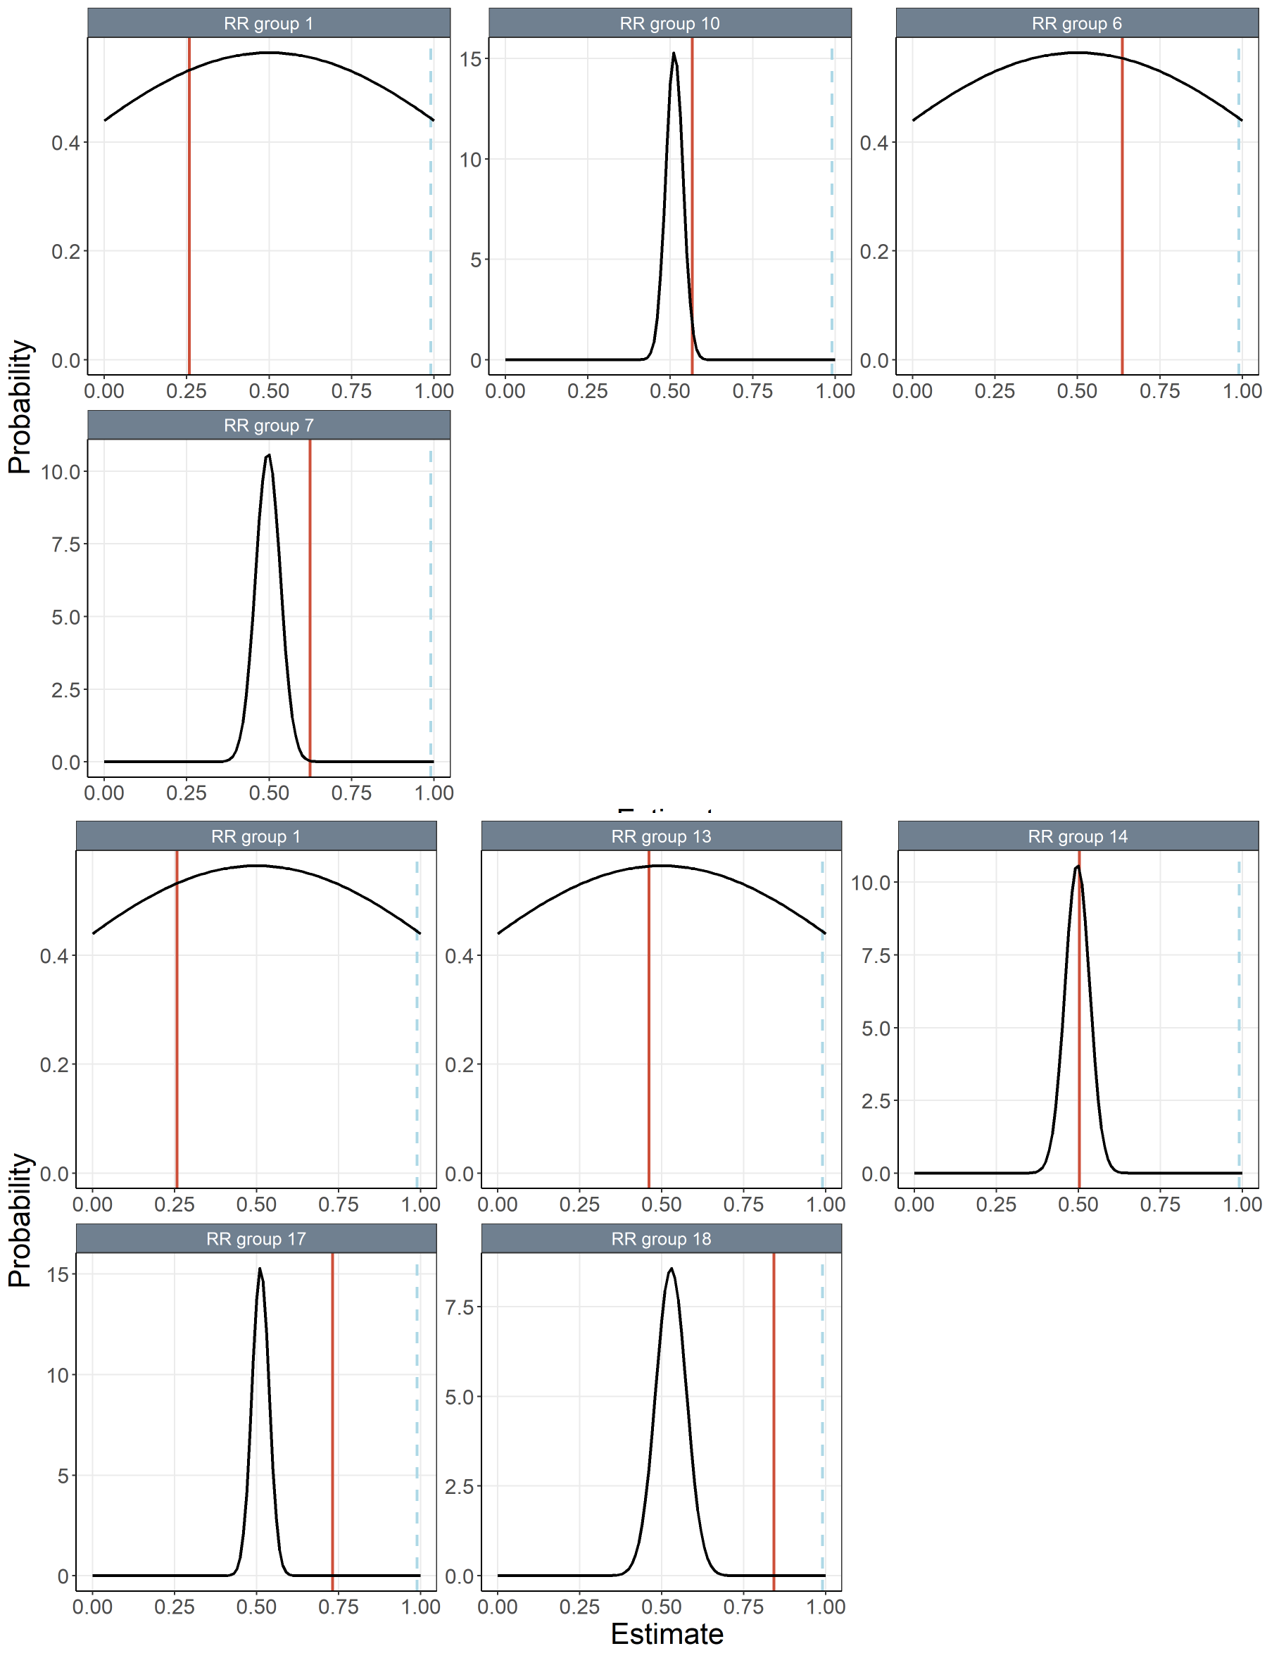
\includegraphics[width=0.8\linewidth,height=\textheight,keepaspectratio]{figures/tag_report_rate_rttp_pttp.png}
%DIFDELCMD <

%DIFDELCMD < }
%DIFDELCMD <

%DIFDELCMD < \caption{\label{fig-tag-report-rates-rttp-pttp}Estimated reporting rates
%DIFDELCMD < for RTTP and PTTP for the diagnostic model (red lines) and the prior
%DIFDELCMD < distribution for each tag reporting rate group (black lines). The upper
%DIFDELCMD < bound (0.99) on the reporting rate parameters is shown as a blue dashed
%DIFDELCMD < line. Reporting rates can be estimated separately for each release
%DIFDELCMD < program and recapture fishery group but in practice are aggregated over
%DIFDELCMD < some recapture groups to reduce dimensionality.}
%DIFDELCMD <

%DIFDELCMD < \end{figure}%%%
\DIFdelend \DIFaddbegin \begin{figure}[H]

\centering{

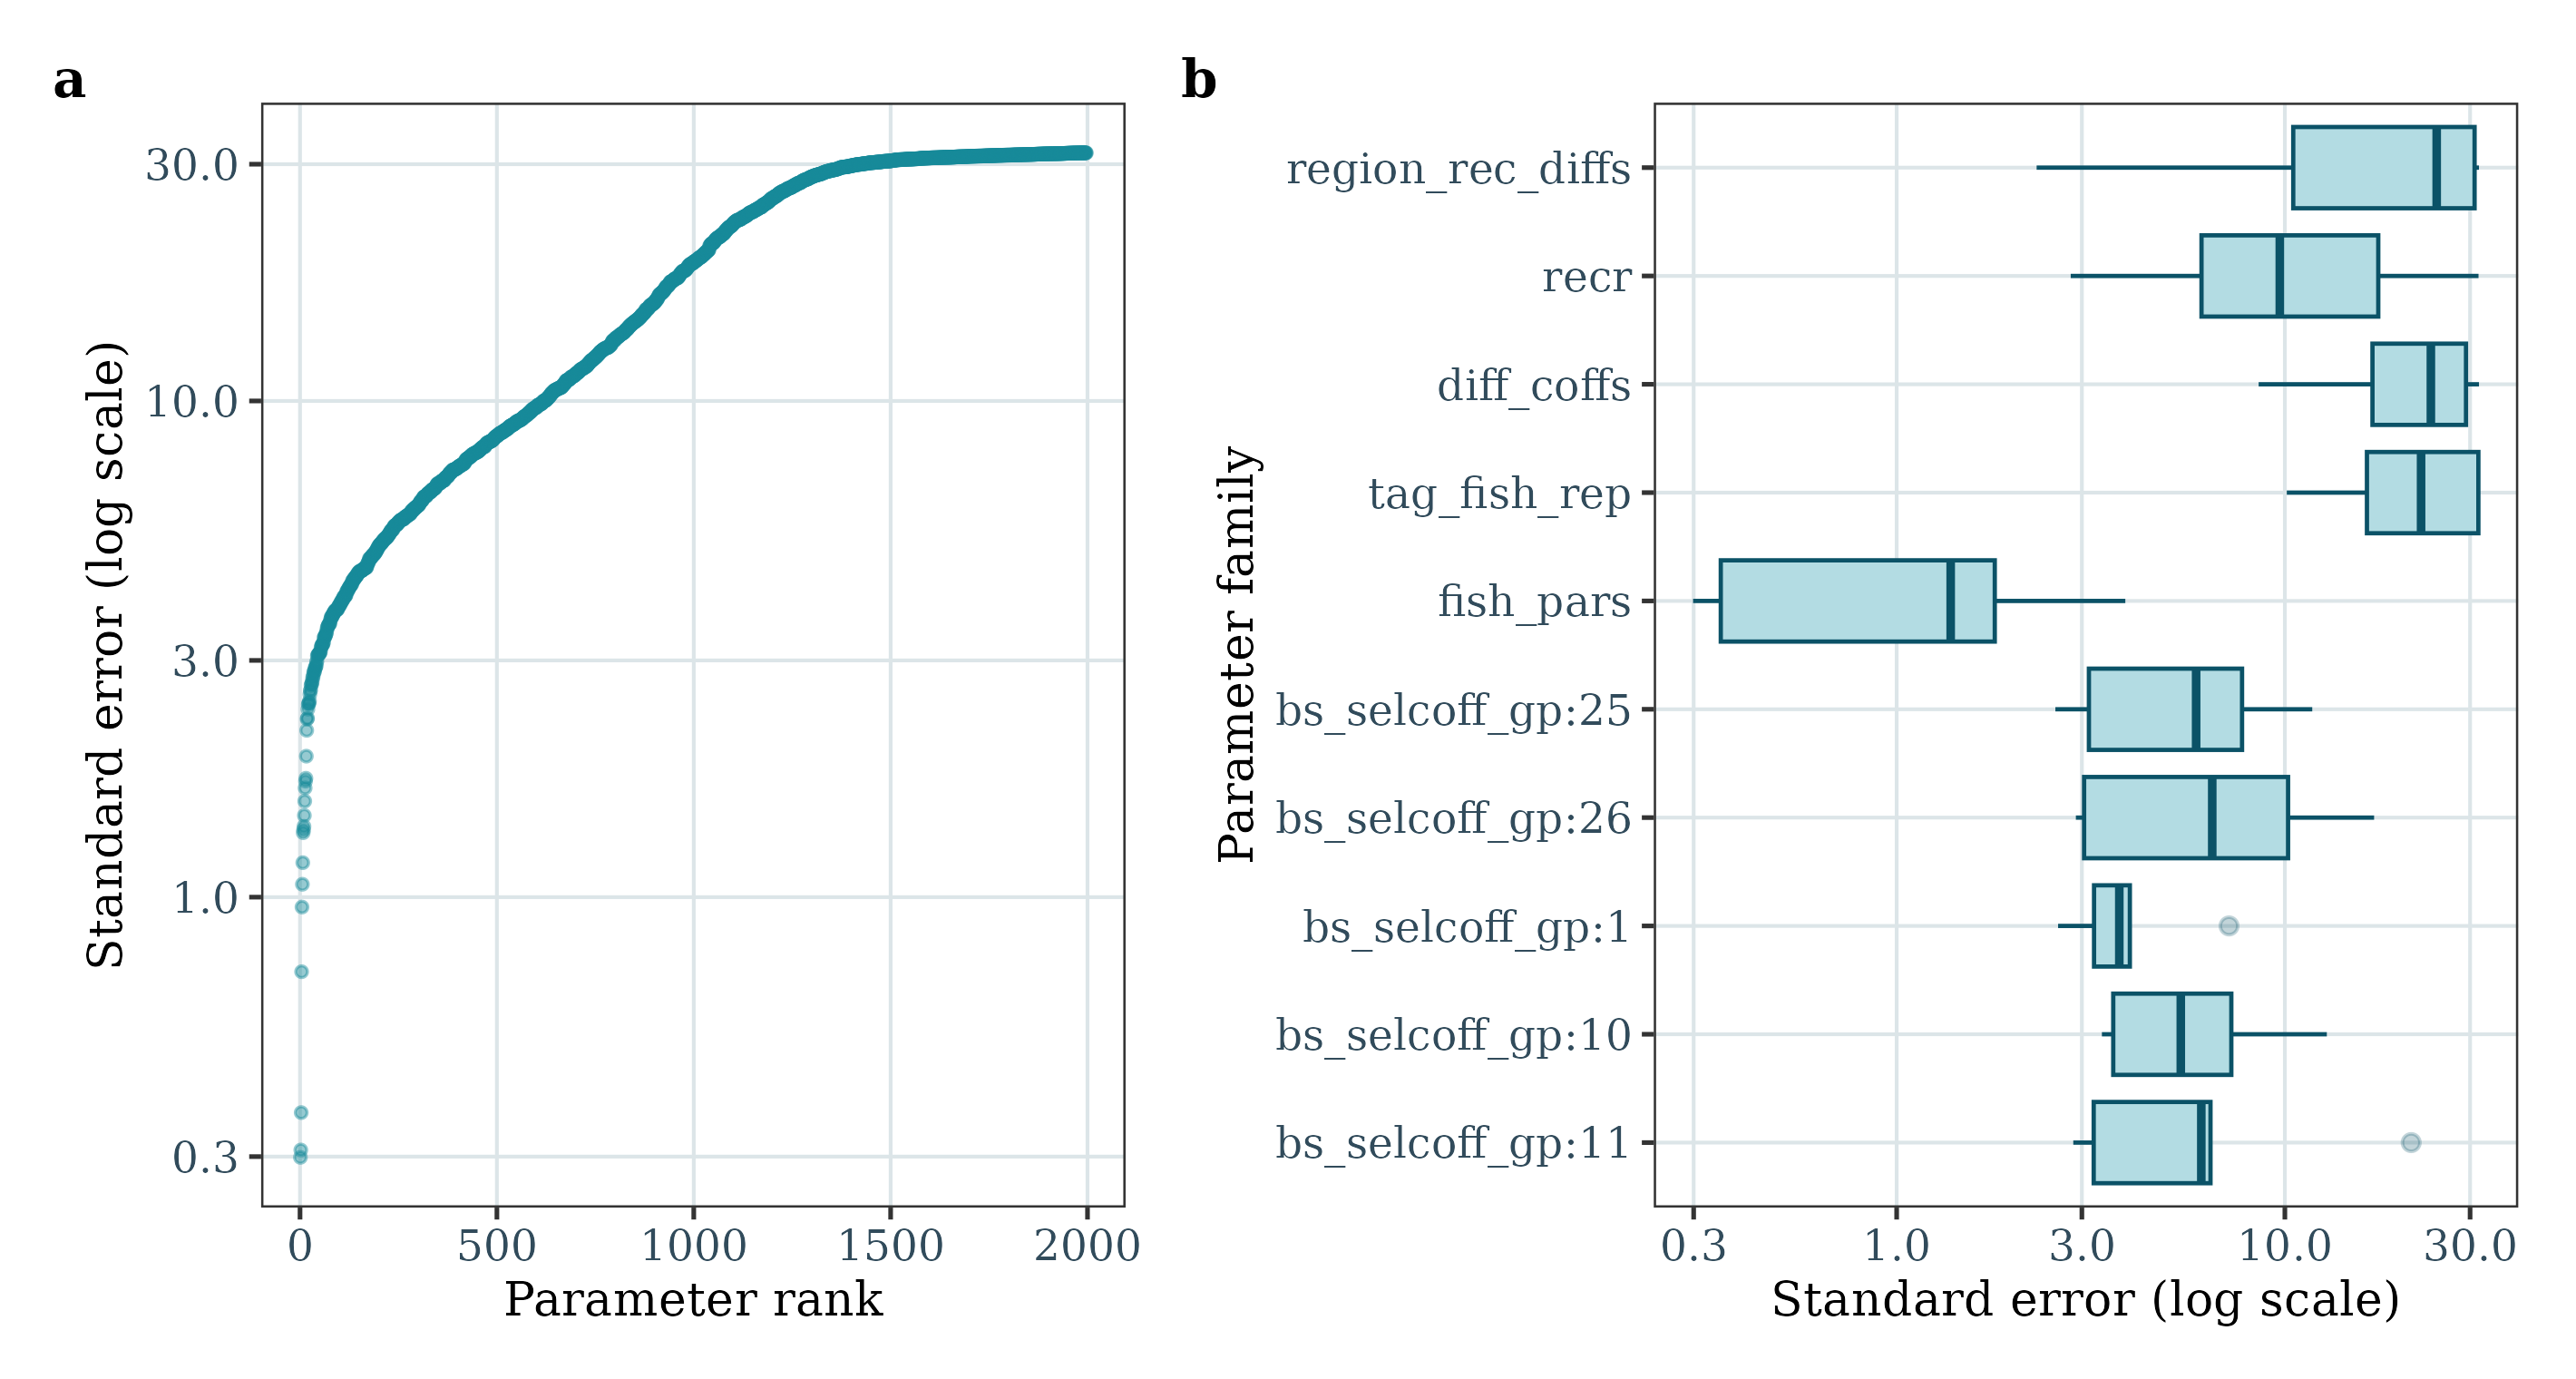
\includegraphics[width=1\linewidth,height=\textheight,keepaspectratio]{figures_new/hessian-parameter-scales.png}

}

\caption{\label{fig-hessian-parameter-scales}Parameter standard errors
derived from the positive-definite inverse Hessian: (a) ordered standard
errors and (b) distributions for the ten most numerous parameter
families. Logarithmic axes show the wide range of estimated parameter
scales.}

\end{figure}\DIFaddend %

\DIFdelbegin %DIFDELCMD < \begin{figure}[H]
%DIFDELCMD <

%DIFDELCMD < \centering{
%DIFDELCMD <

%DIFDELCMD < 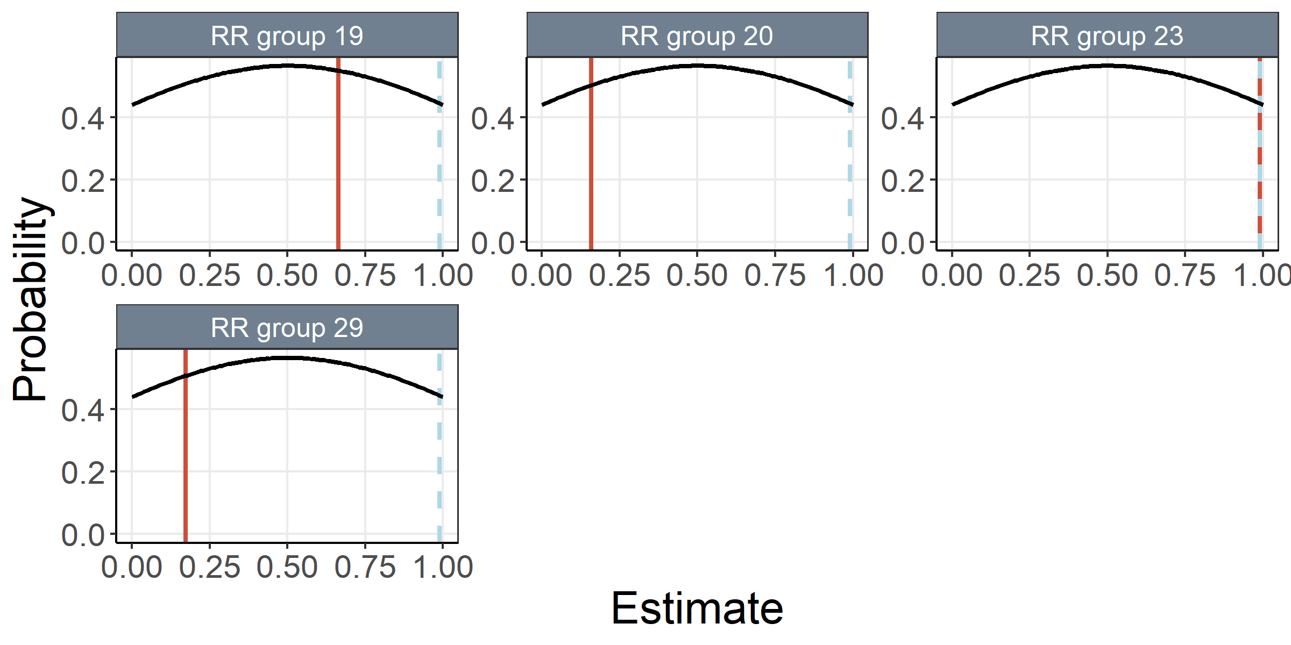
\includegraphics[width=1\linewidth,height=\textheight,keepaspectratio]{figures/tag_report_rate_jptp.png}
%DIFDELCMD <

%DIFDELCMD < }
%DIFDELCMD <

%DIFDELCMD < \caption{\label{fig-tag-report-rates-jtpt}Estimated reporting rates for
%DIFDELCMD < JPTP for the diagnostic model (red lines) and the prior distribution for
%DIFDELCMD < each tag reporting rate group (black lines). The upper bound (0.99) on
%DIFDELCMD < the reporting rate parameters is shown as a blue dashed line. Reporting
%DIFDELCMD < rates can be estimated separately for each release program and recapture
%DIFDELCMD < fishery group but in practice are aggregated over some recapture groups
%DIFDELCMD < to reduce dimensionality.}
%DIFDELCMD <

%DIFDELCMD < \end{figure}%%%
\DIFdelend \DIFaddbegin \begin{figure}[H]

\centering{

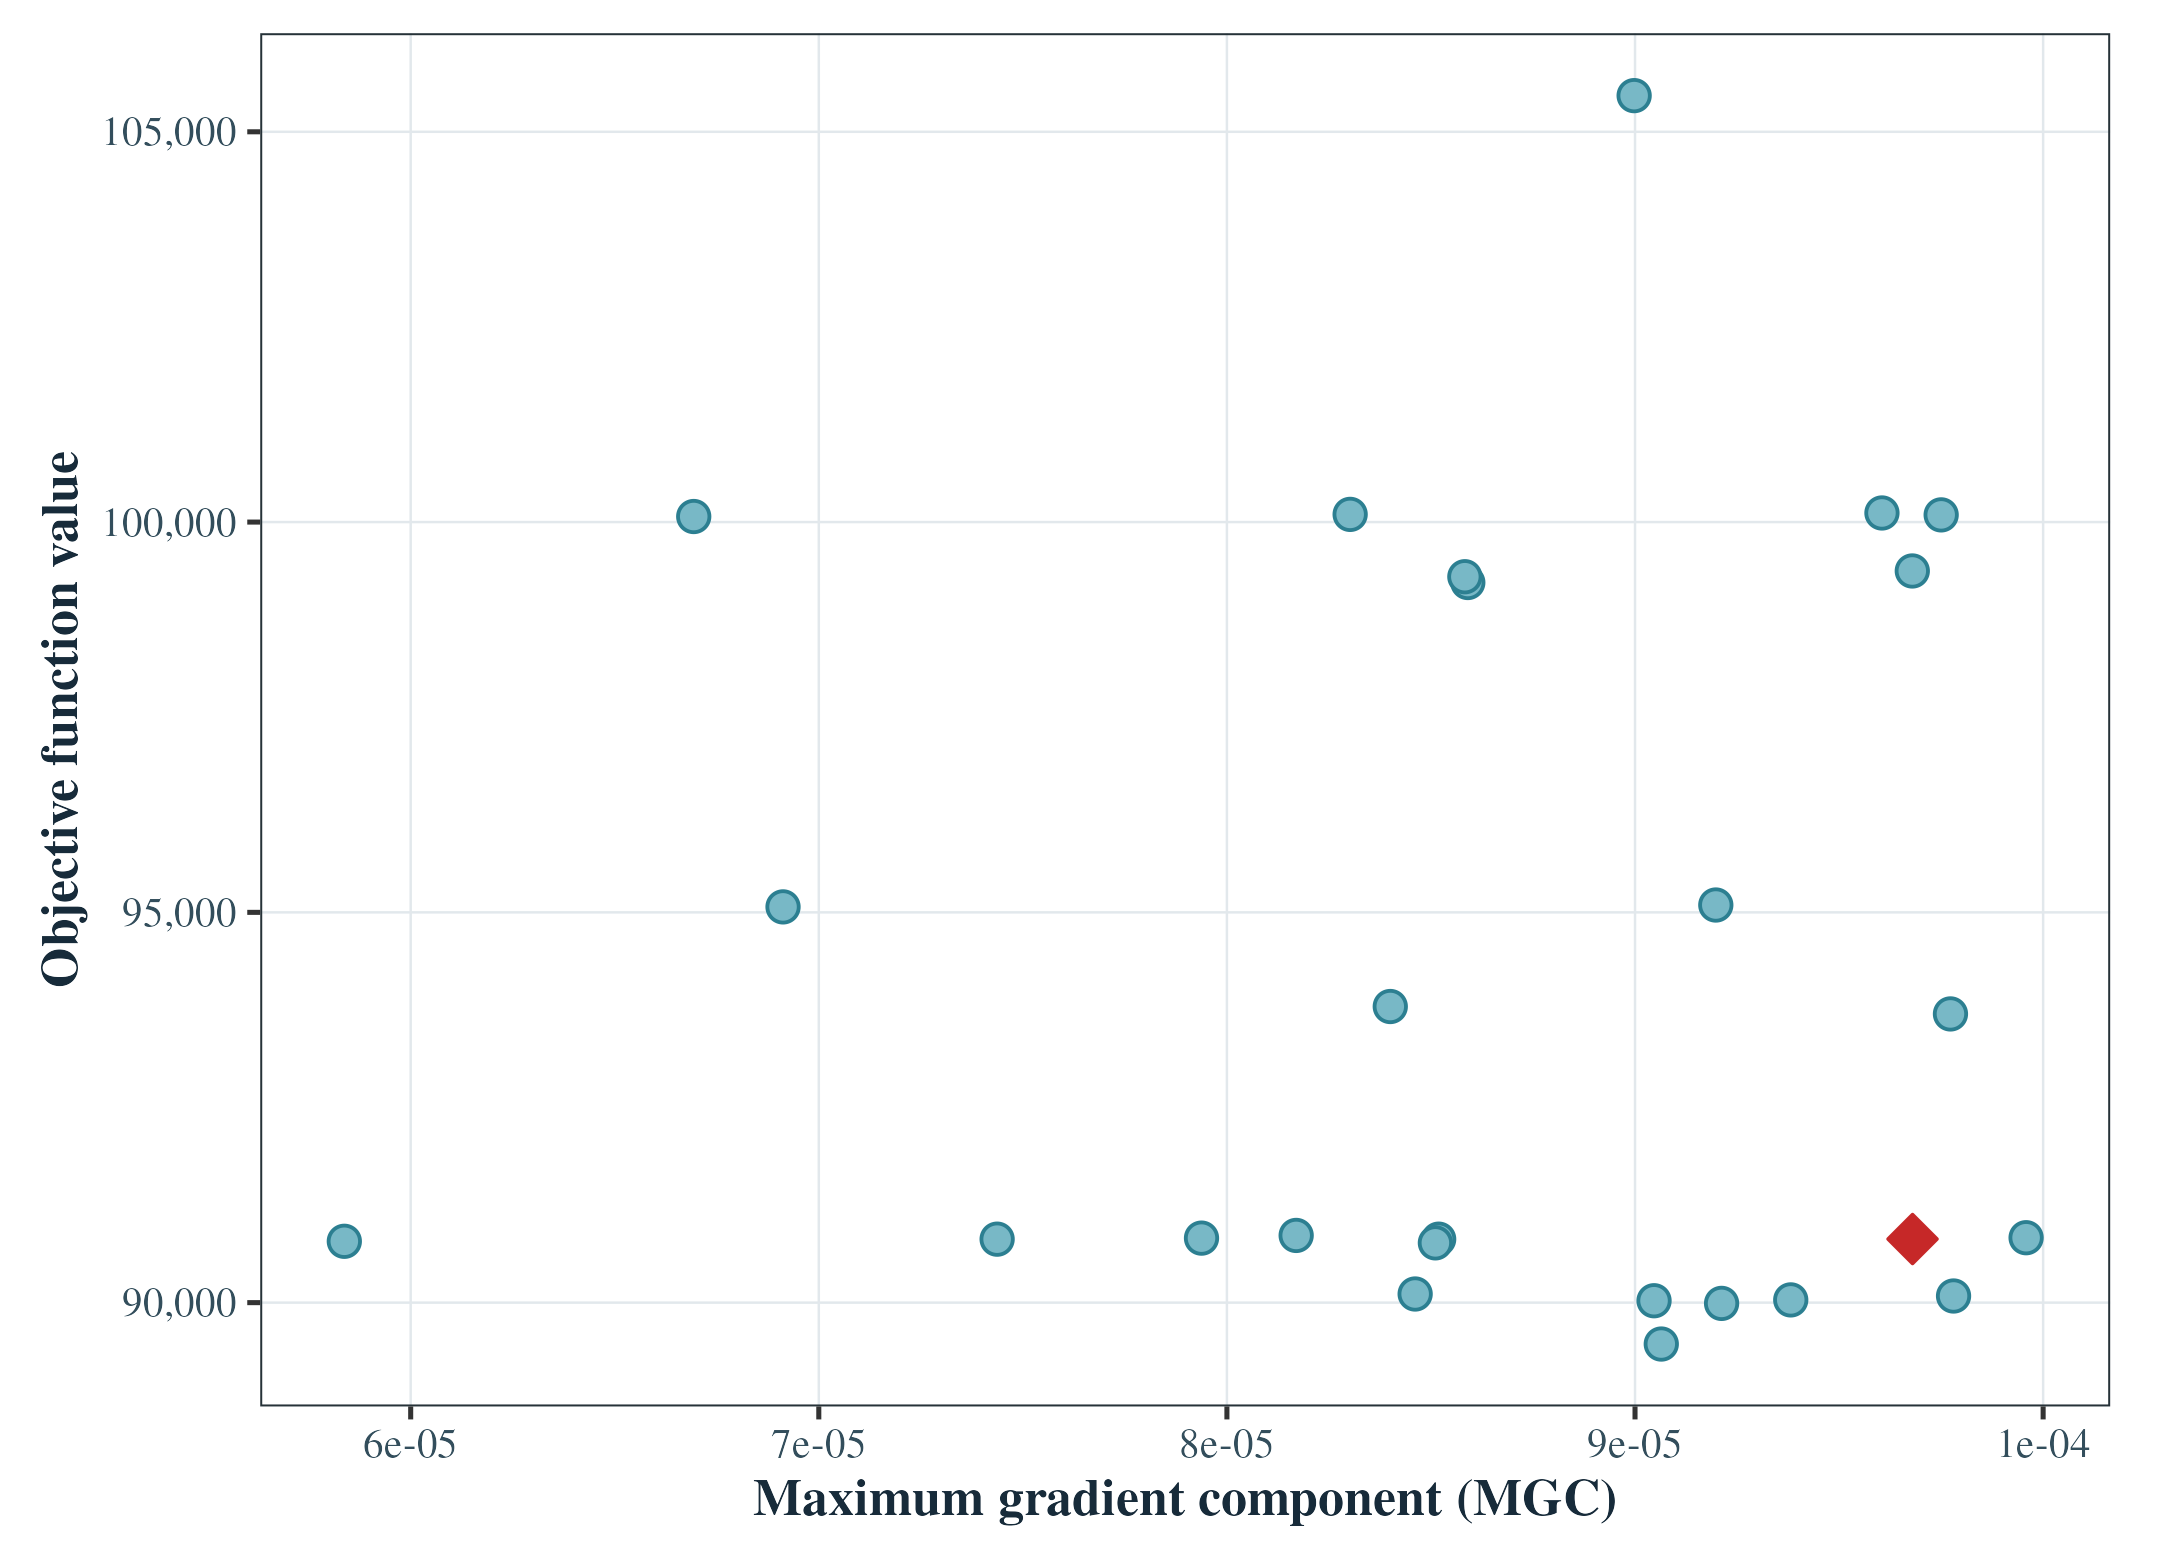
\includegraphics[width=1\linewidth,height=\textheight,keepaspectratio]{figures/jitter_scatter_plot.png}

}

\caption{\label{fig-jitter-scatter-plot}Jitter convergence diagnostics
for the diagnostic model. Each circle represents one of the 25 retained
jitter fits and the red diamond identifies the diagnostic model without
jitter. Retained fits had a maximum gradient component no greater than
\(1.0 \times 10^{-4}\); lower objective-function values indicate
improved fit. Open the
\href{https://pacificcommunity.github.io/ofp-sam-bet-2026-jitter/jitter-report.html}{interactive
jitter report}.}

\end{figure}\DIFaddend %

\DIFdelbegin %DIFDELCMD < \begin{figure}[H]
%DIFDELCMD <

%DIFDELCMD < \centering{
%DIFDELCMD <

%DIFDELCMD < 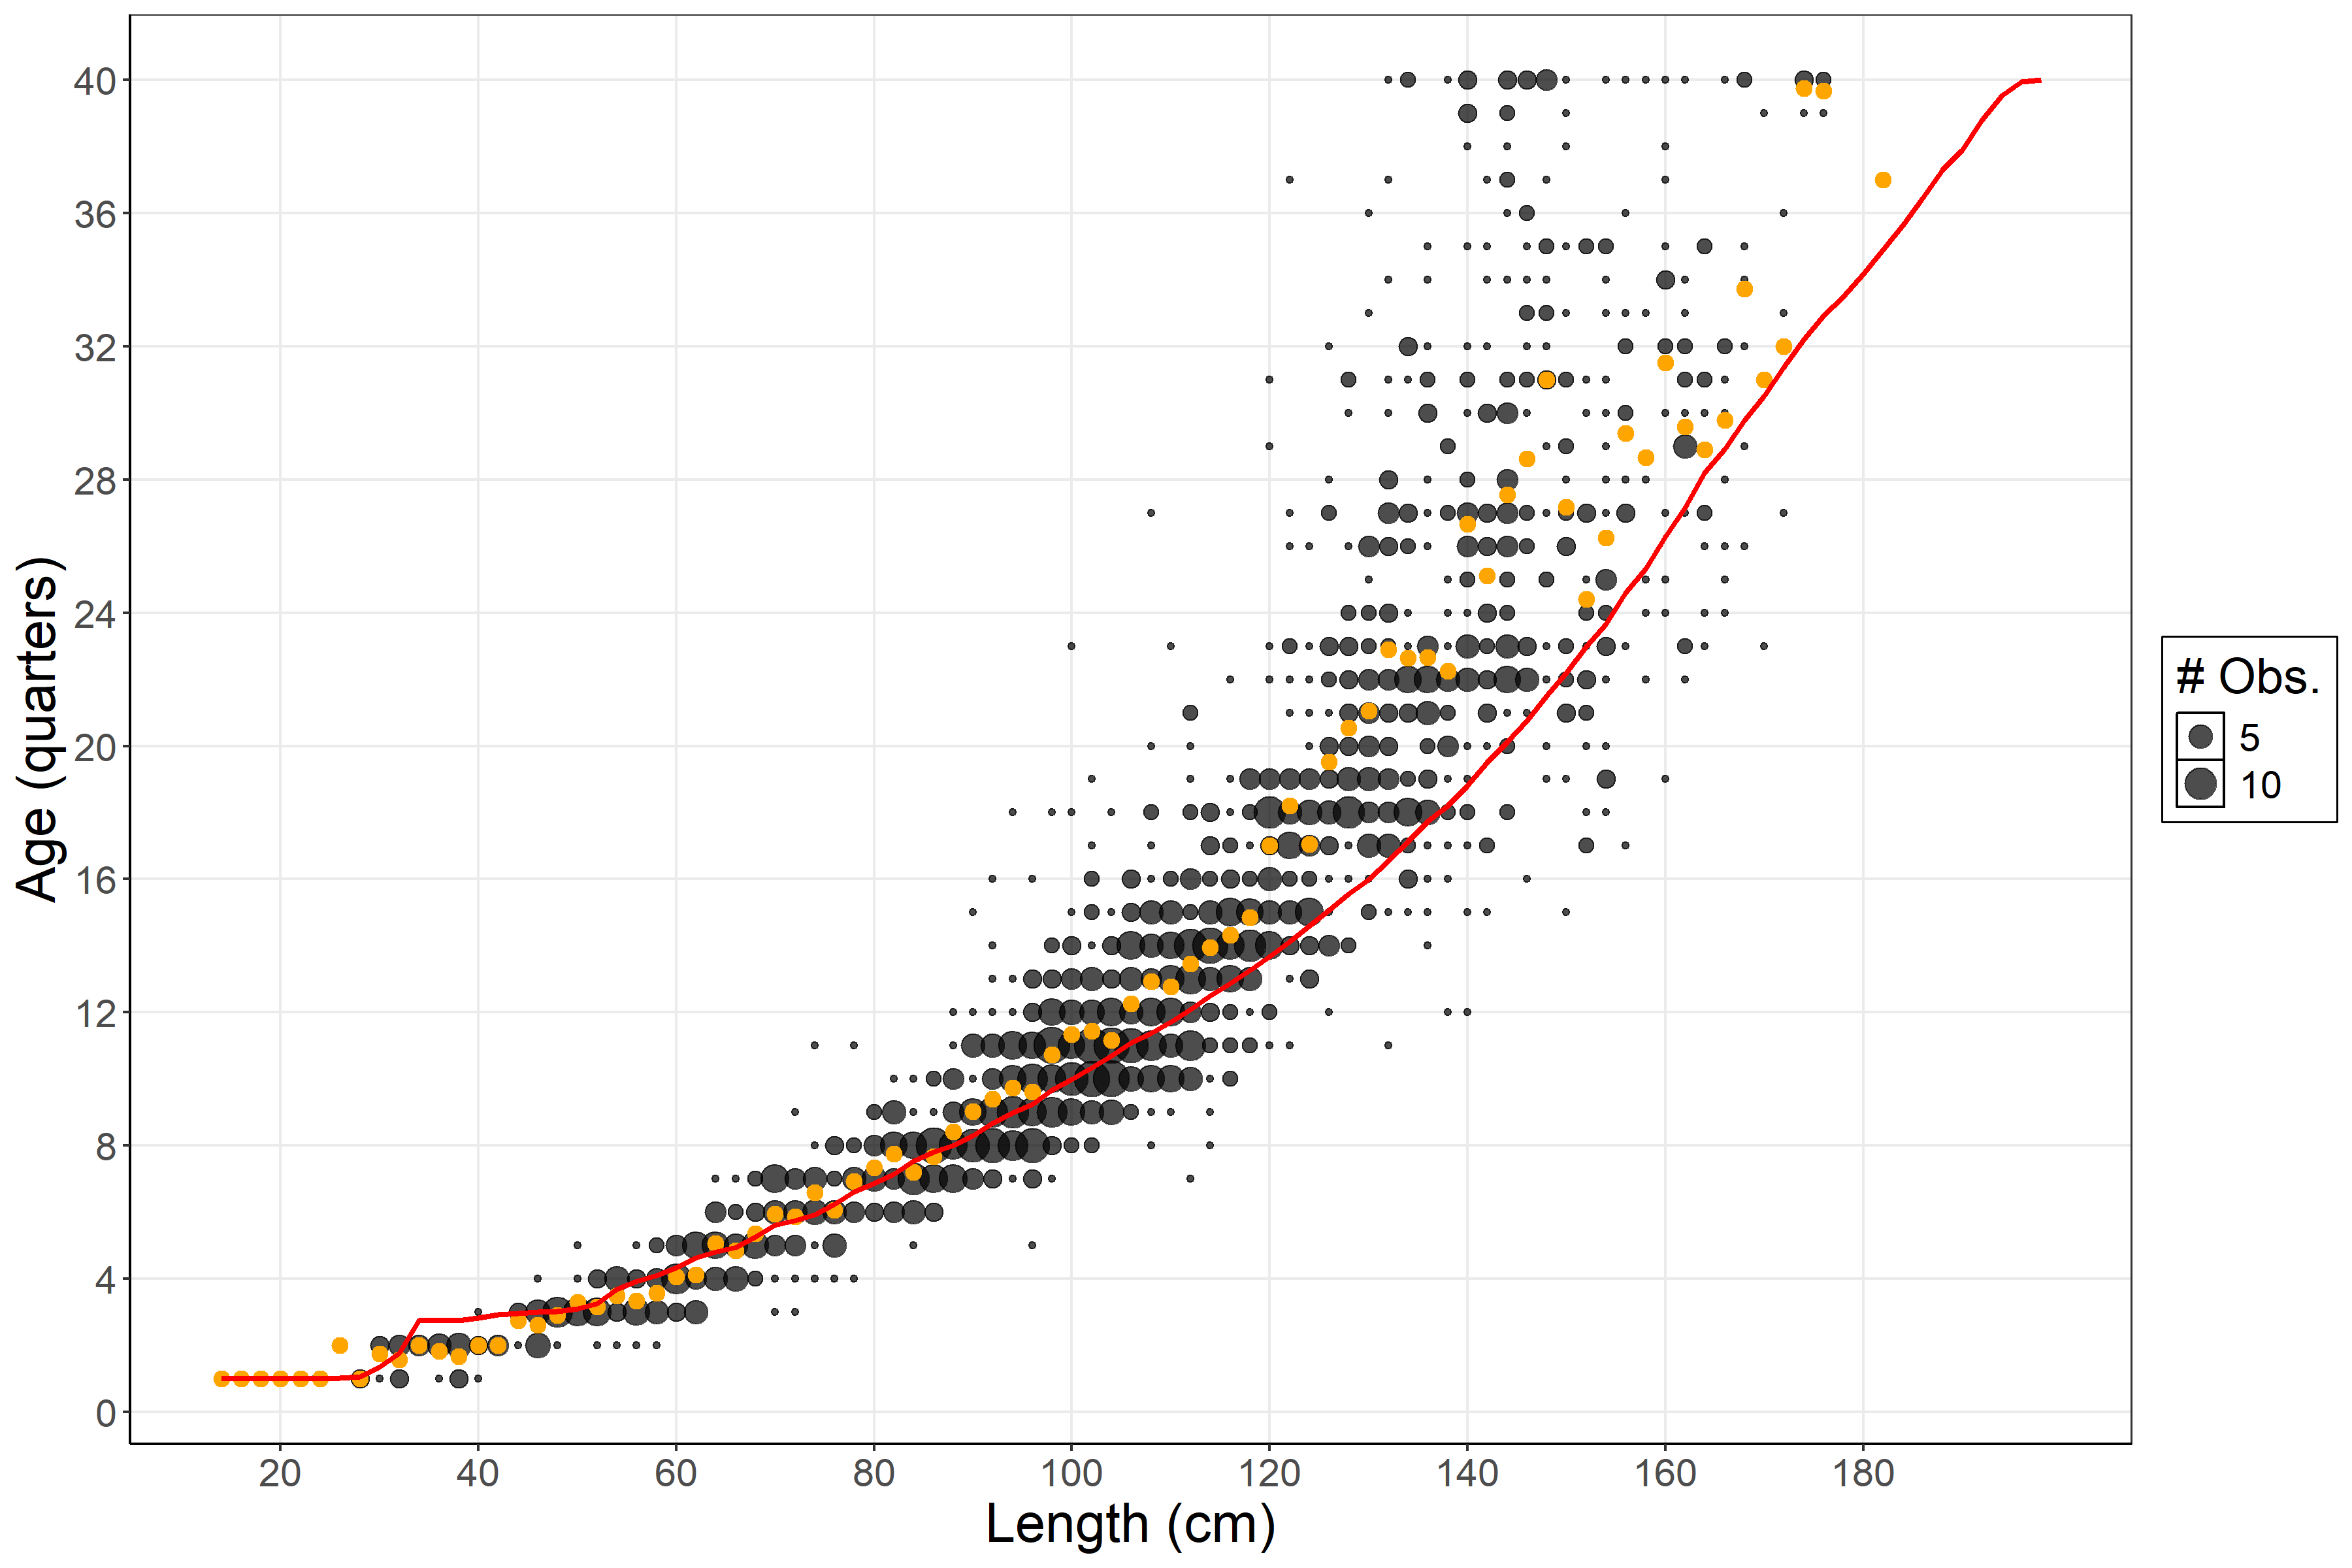
\includegraphics[width=0.85\linewidth,height=\textheight,keepaspectratio]{figures/caal_aggregate_fits.png}
%DIFDELCMD <

%DIFDELCMD < }
%DIFDELCMD <

%DIFDELCMD < \caption{\label{fig-caal-fits}Model estimated median age at length
%DIFDELCMD < (orange line), versus observed age at length (black circles), and median
%DIFDELCMD < observed age at lengths (orange circles), aggregate across all samples
%DIFDELCMD < (top) and by model regions (bottom), The distribution of observed age at
%DIFDELCMD < length is viewed by the vertical distribution of the black dots.}
%DIFDELCMD <

%DIFDELCMD < \end{figure}%%%
\DIFdelend \DIFaddbegin \begin{figure}[H]

\centering{

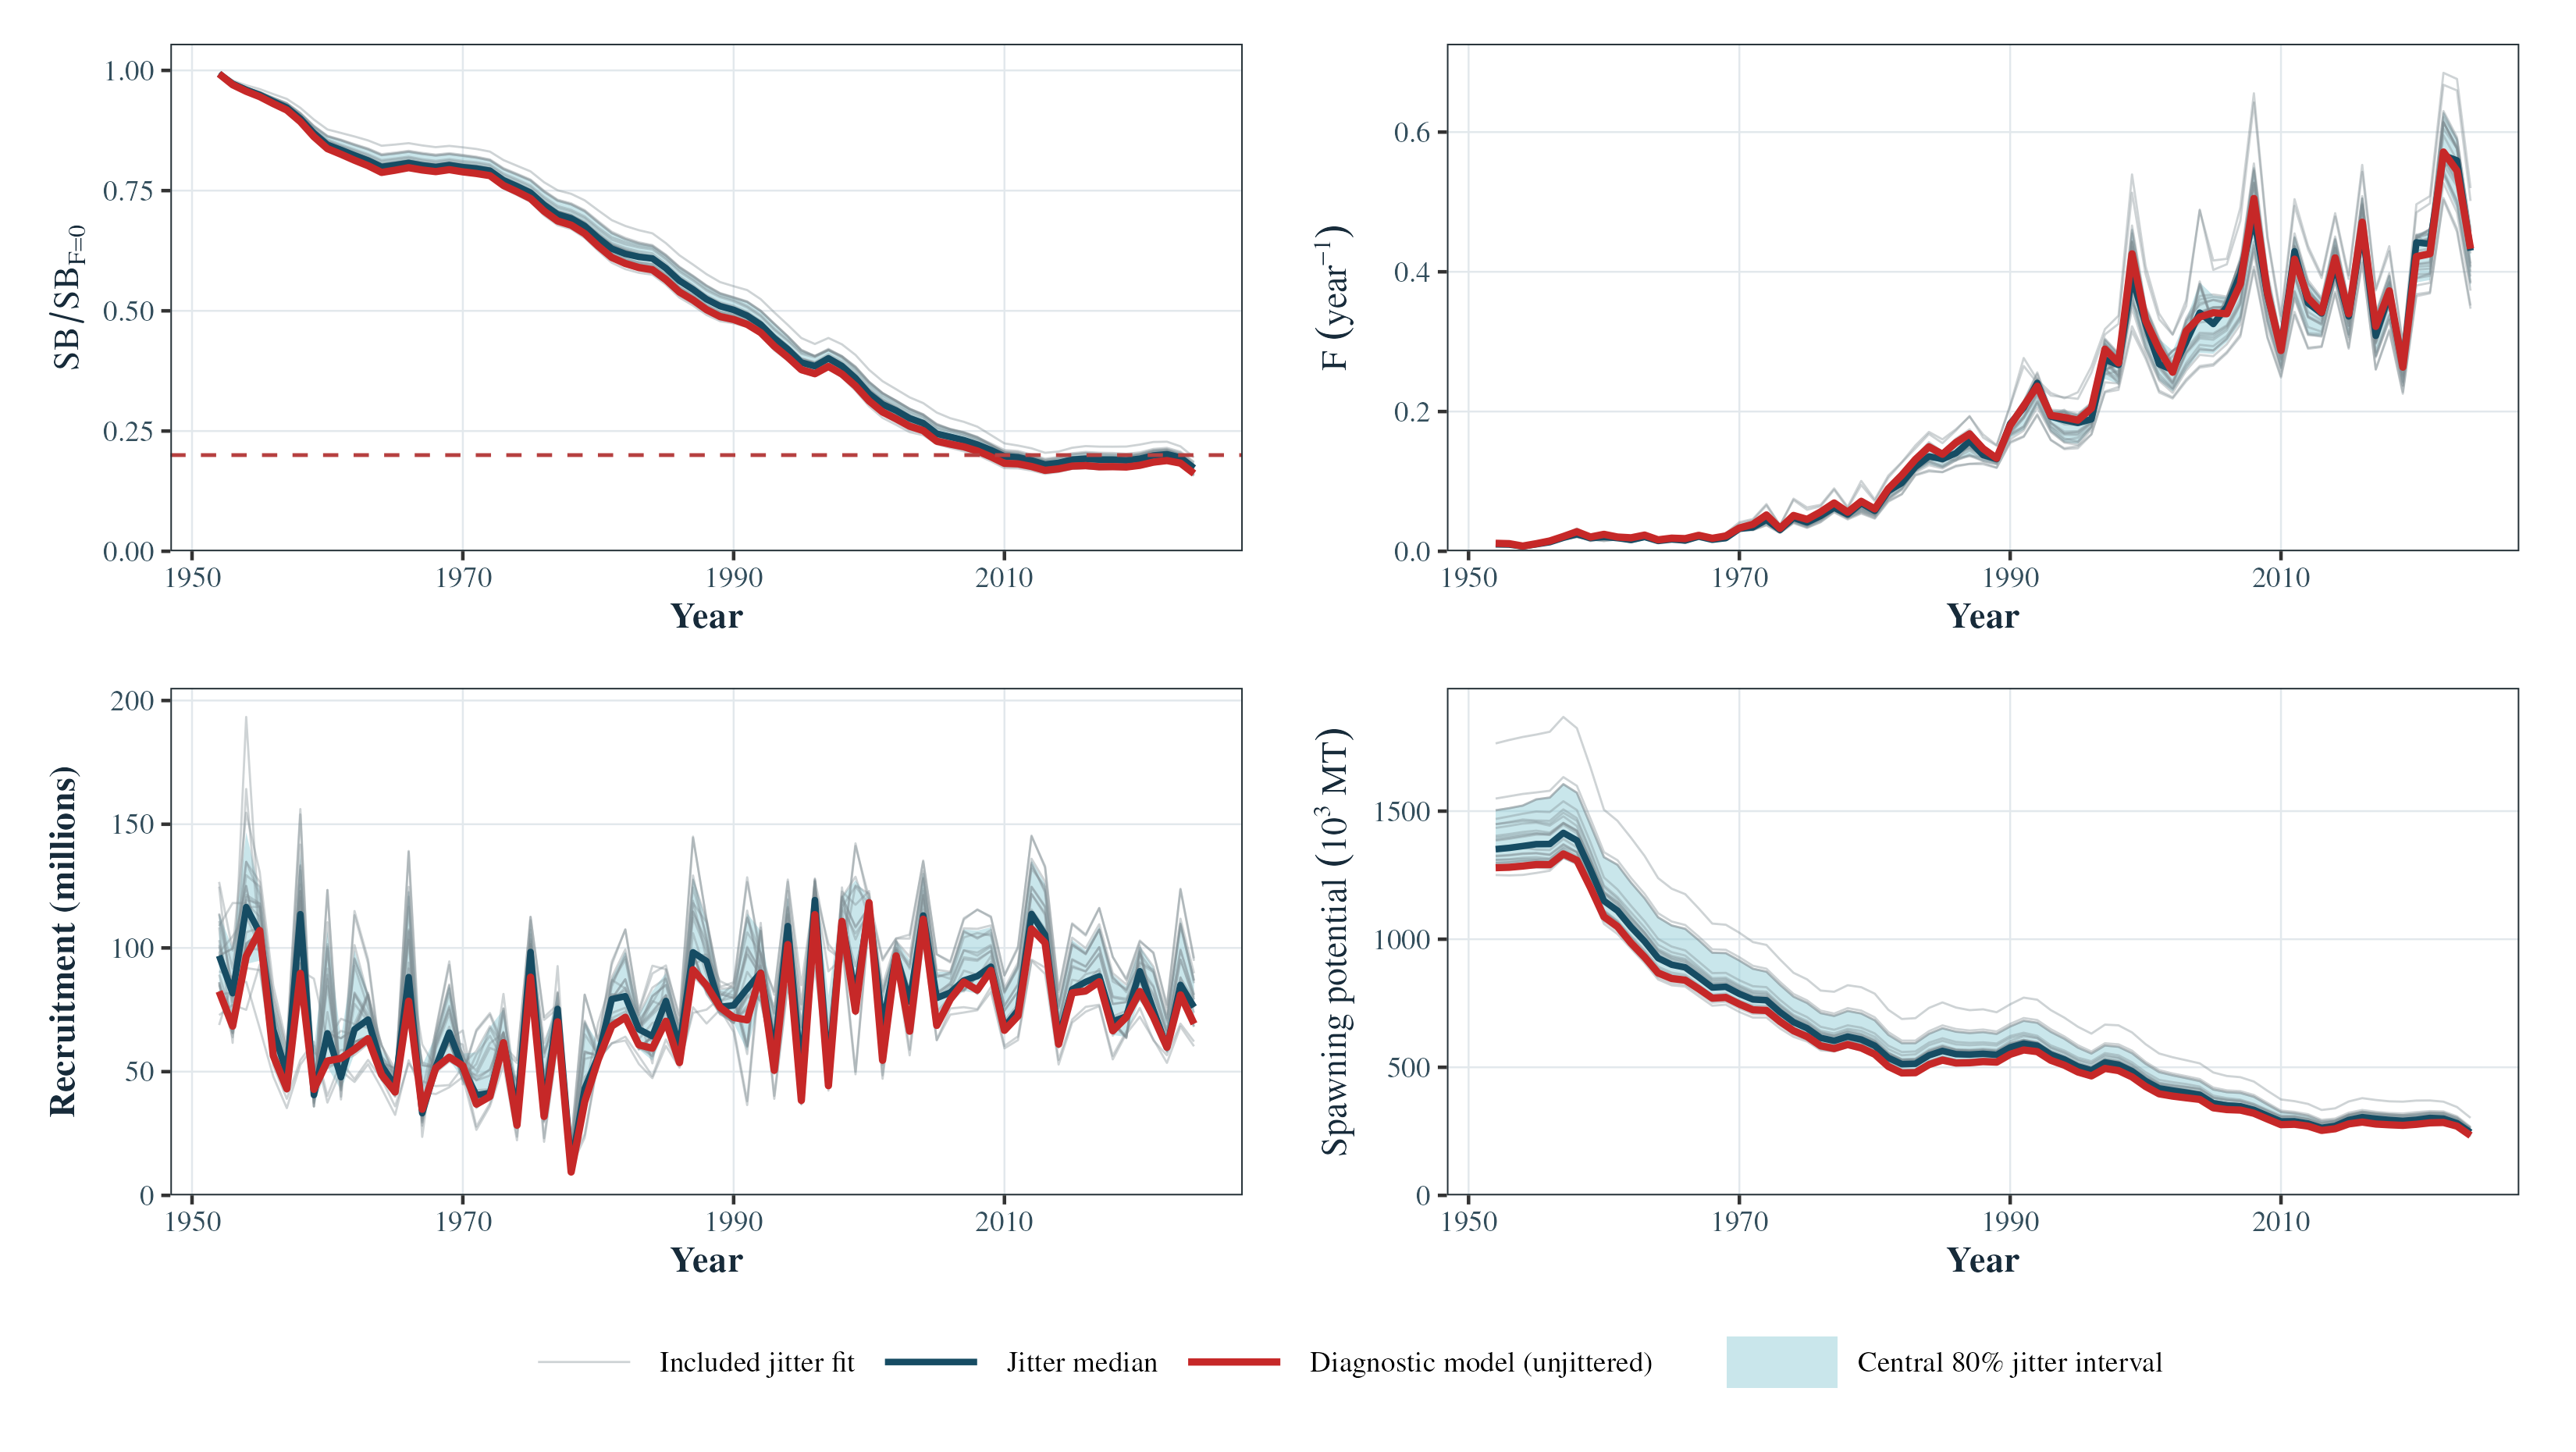
\includegraphics[width=1\linewidth,height=\textheight,keepaspectratio]{figures/jitter_derived_values_diag_panel.png}

}

\caption{\label{fig-jitter-derived-values-diag-panel}Annual derived
quantities across the 25 retained jitter fits. Thin grey-blue lines are
individual fits, the shaded band is the pointwise central 80\% interval,
the dark line is the jitter median and the red line is the diagnostic
model without jitter. Recruitment is in millions of fish and spawning
potential is in thousand metric tonnes.}

\end{figure}\DIFaddend %

\DIFdelbegin %DIFDELCMD < \begin{figure}[H]
%DIFDELCMD <

%DIFDELCMD < \centering{
%DIFDELCMD <

%DIFDELCMD < 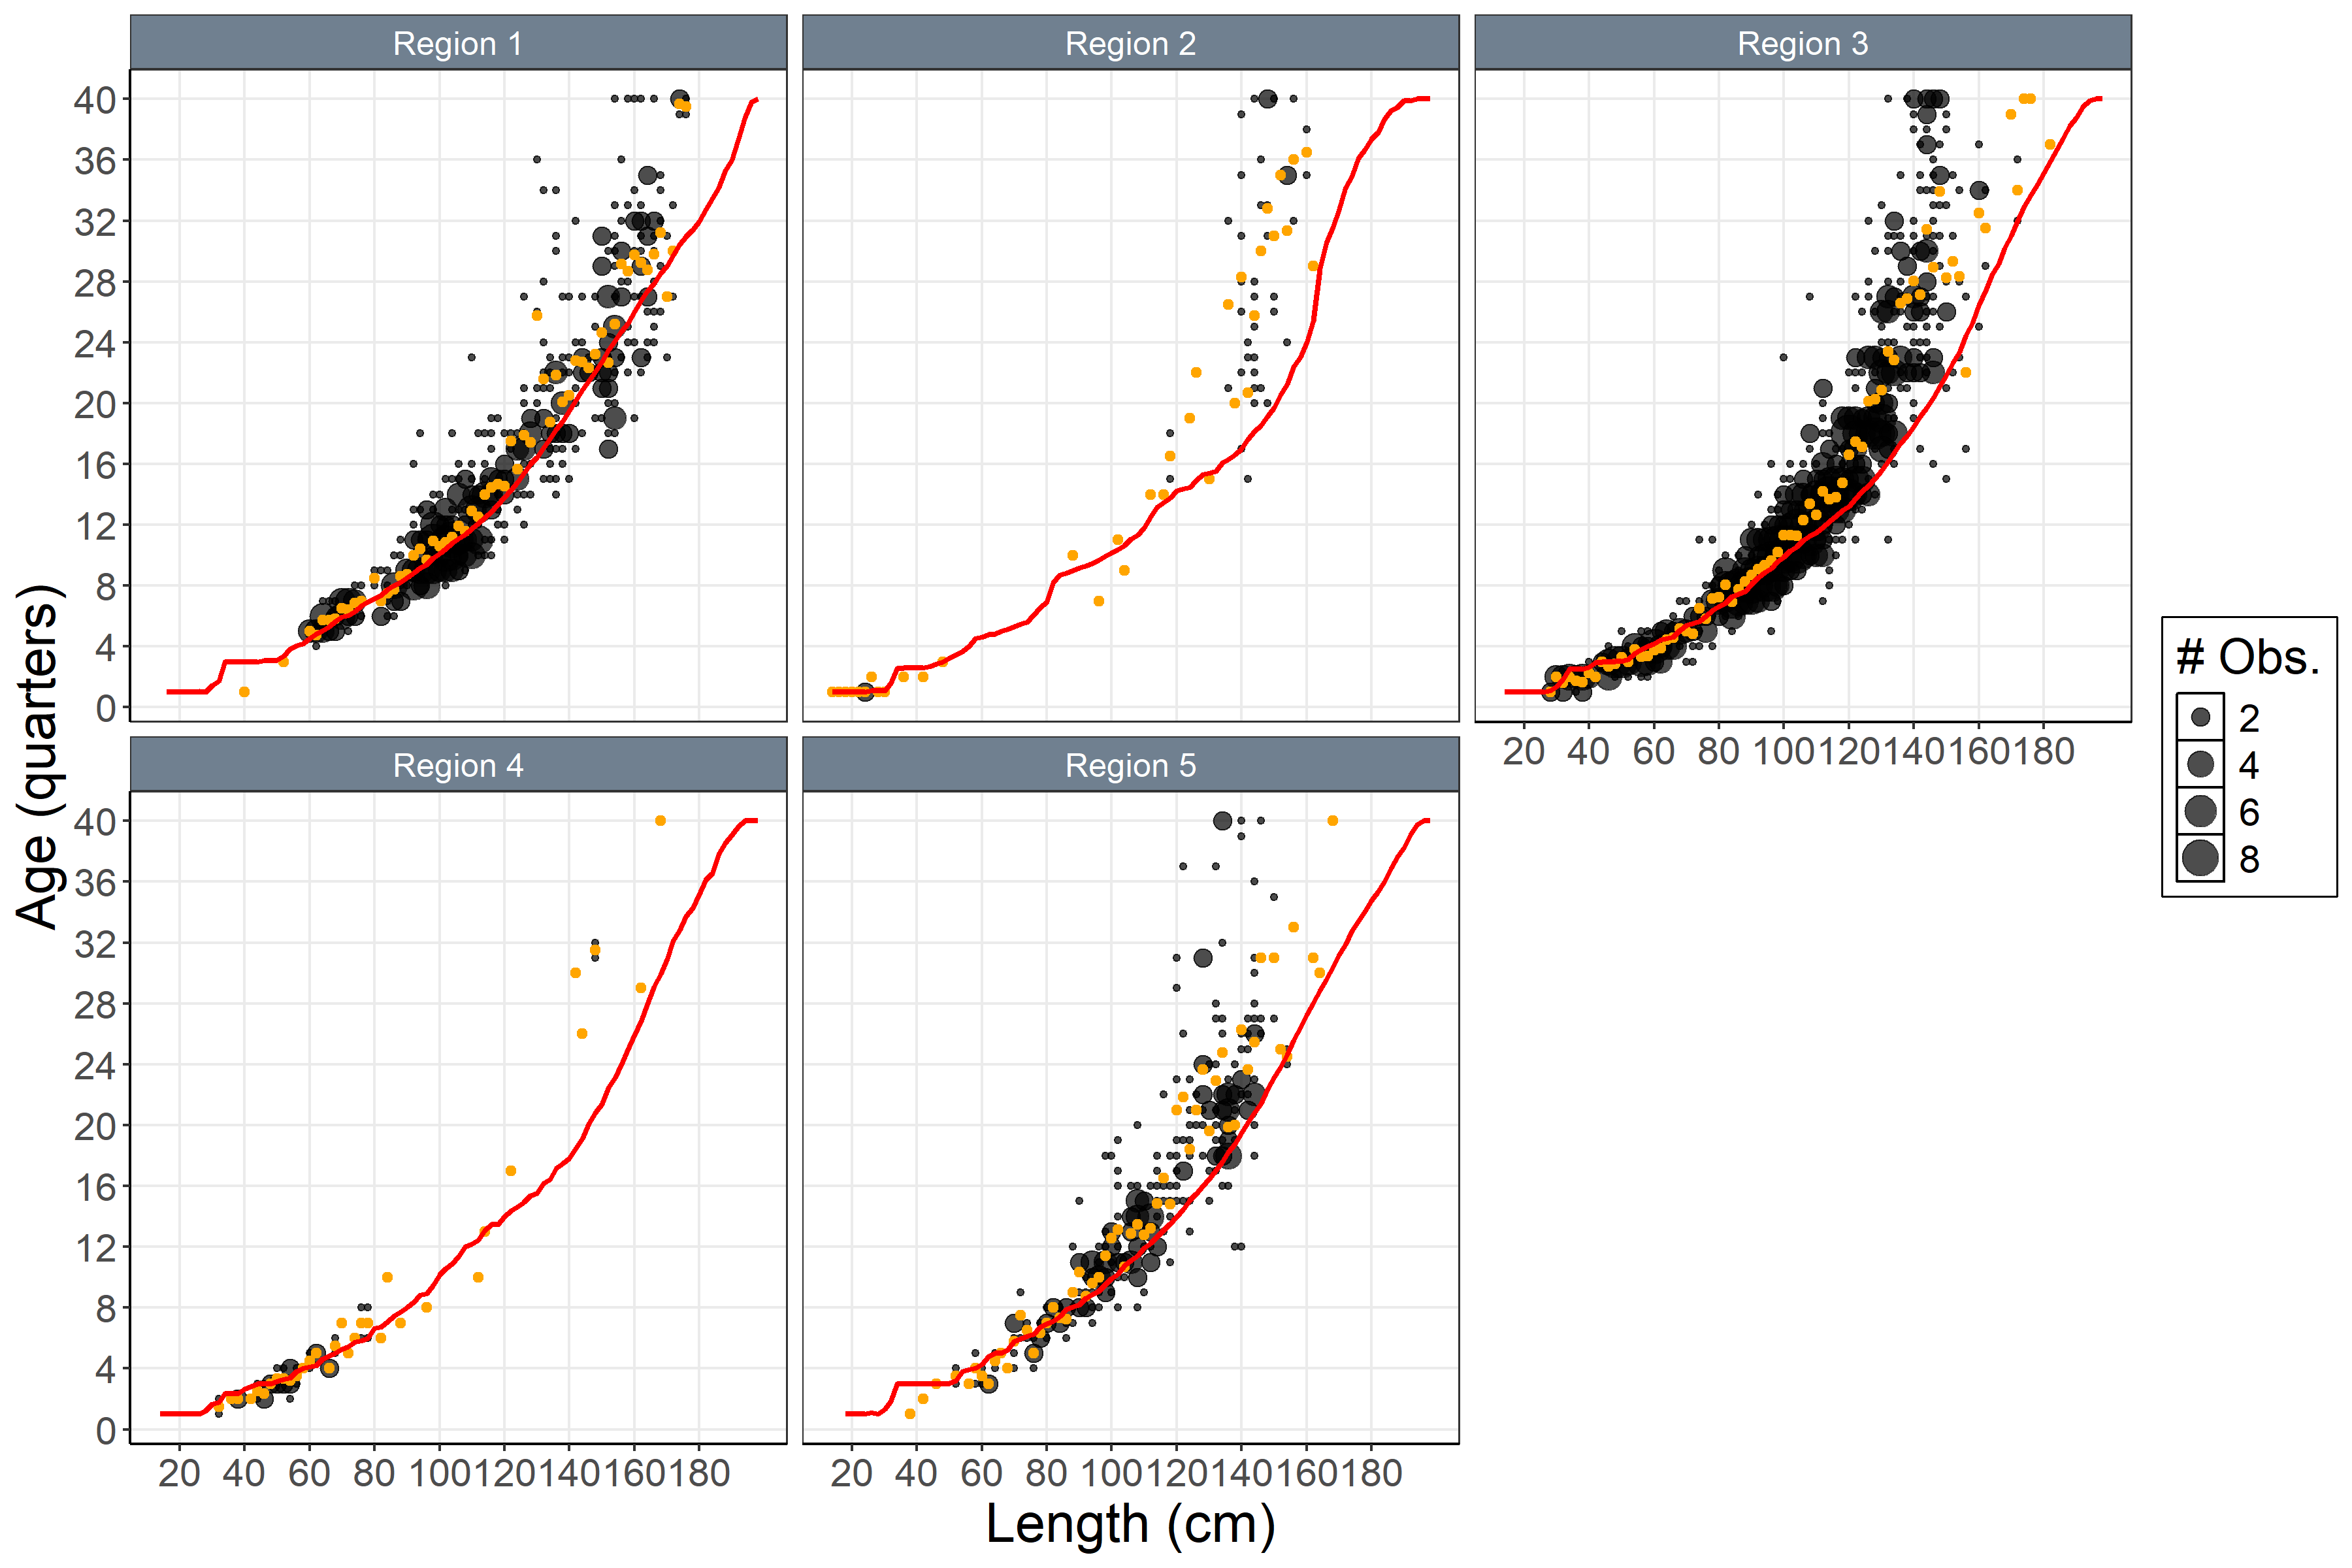
\includegraphics[width=0.85\linewidth,height=\textheight,keepaspectratio]{figures/caal_fits_regions.png}
%DIFDELCMD <

%DIFDELCMD < }
%DIFDELCMD <

%DIFDELCMD < \caption{\label{fig-caal-fits-regions}Model estimated median age at
%DIFDELCMD < length (orange line), versus observed age at length (black circles), and
%DIFDELCMD < median observed age at lengths (orange circles), aggregate across all
%DIFDELCMD < samples (top) and by model regions (bottom), The distribution of
%DIFDELCMD < observed age at length is viewed by the vertical distribution of the
%DIFDELCMD < black dots.}
%DIFDELCMD <

%DIFDELCMD < \end{figure}%%%
\DIFdelend \DIFaddbegin \begin{figure}[H]

\centering{

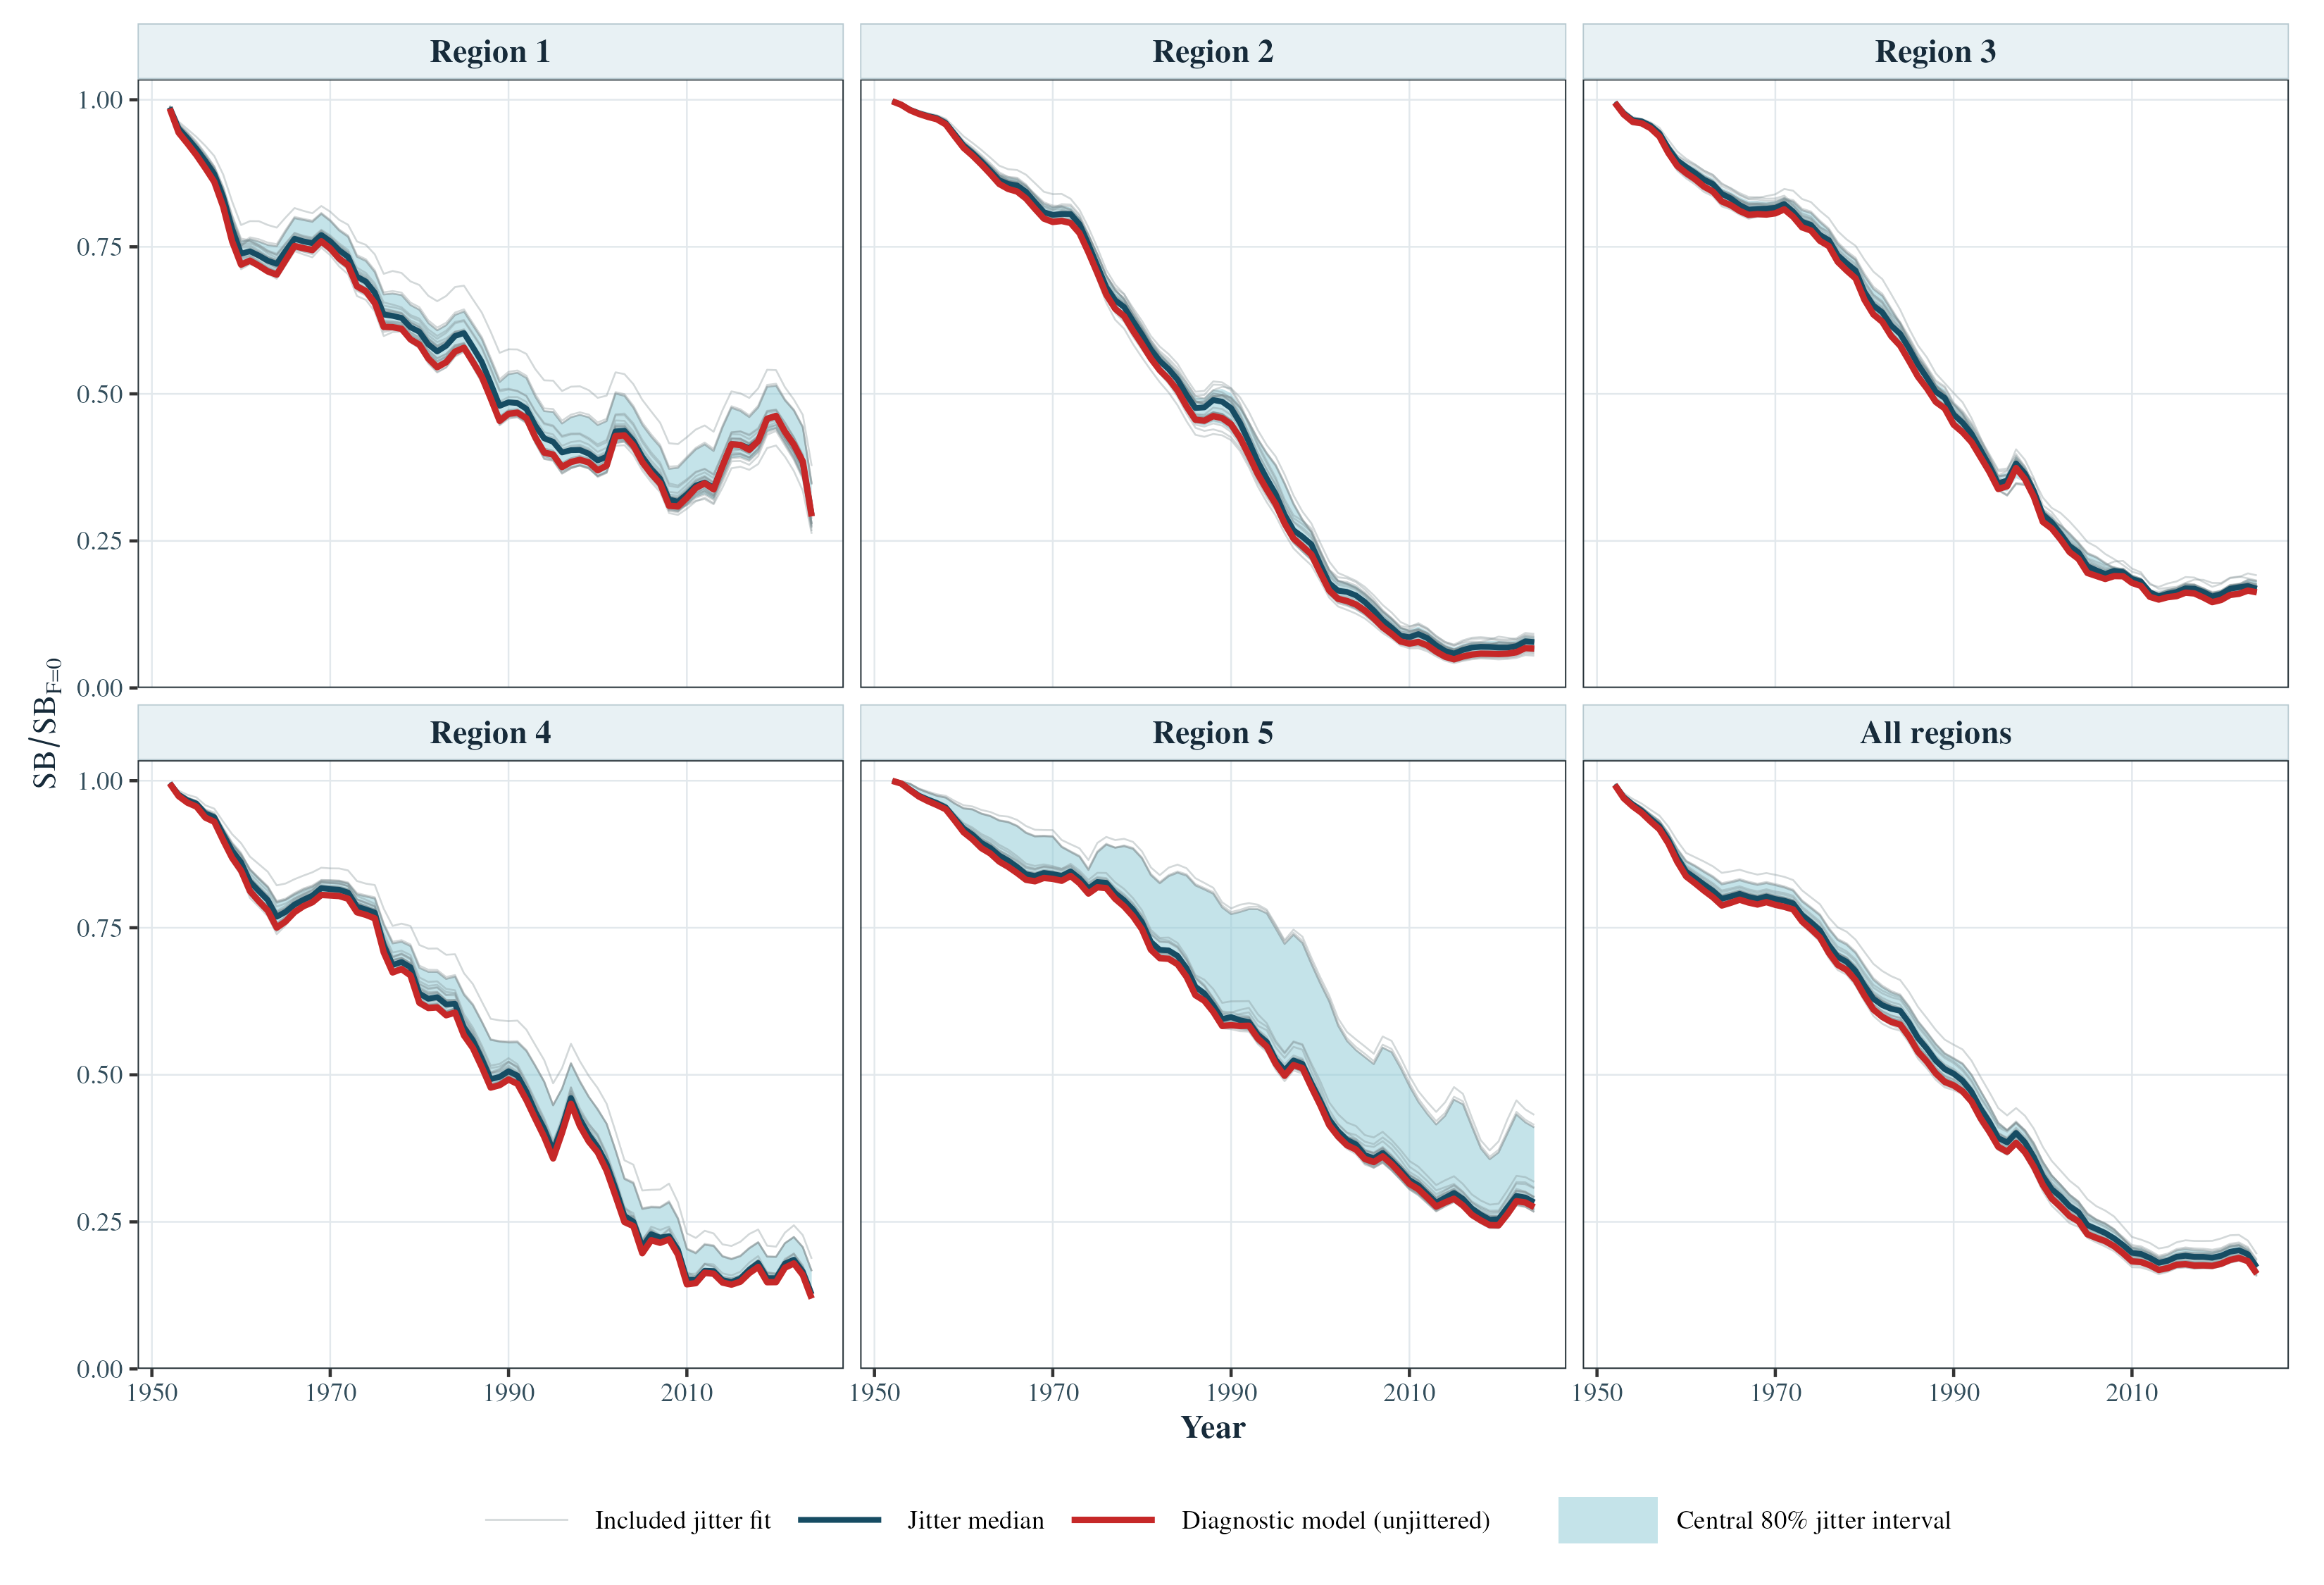
\includegraphics[width=1\linewidth,height=\textheight,keepaspectratio]{figures/jitter_regional_depletion.png}

}

\caption{\label{fig-jitter-regional-depletion}Regional and all-region
depletion trajectories across the 25 retained jitter fits. Thin
grey-blue lines are individual fits, the shaded band is the pointwise
central 80\% interval, the dark line is the jitter median and the red
line is the diagnostic model without jitter.}

\end{figure}\DIFaddend %

\DIFdelbegin %DIFDELCMD < \begin{figure}[H]
%DIFDELCMD <

%DIFDELCMD < \centering{
%DIFDELCMD <

%DIFDELCMD < 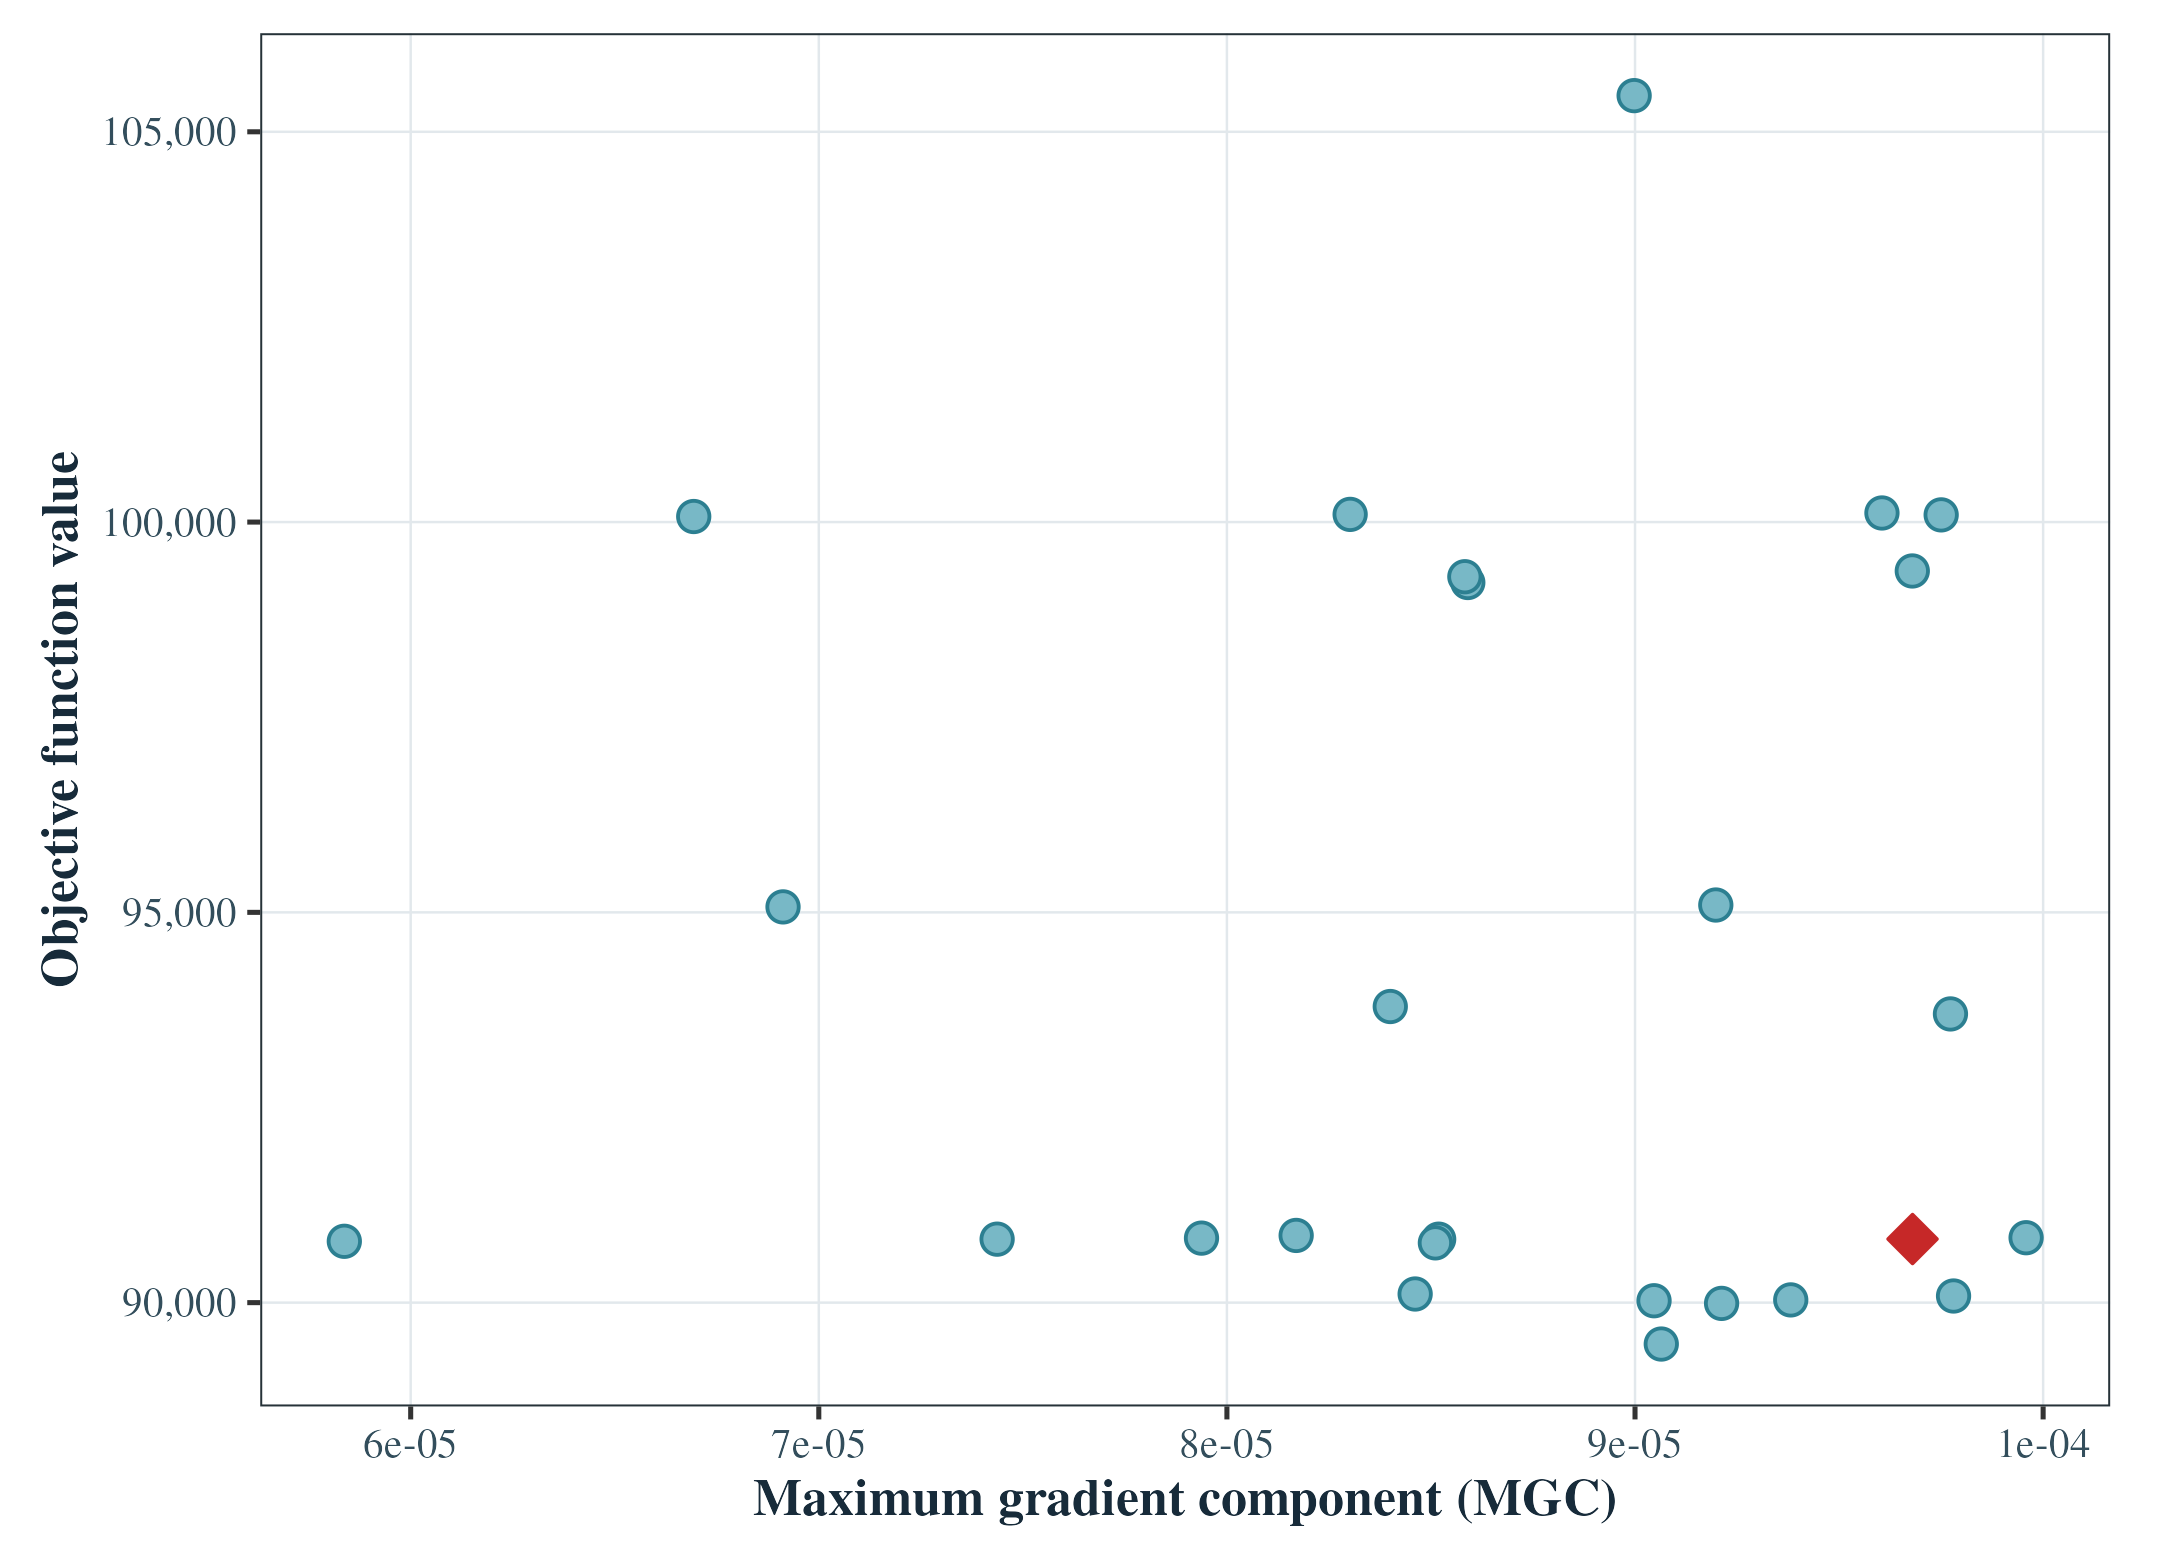
\includegraphics[width=1\linewidth,height=\textheight,keepaspectratio]{figures/jitter_scatter_plot.png}
%DIFDELCMD <

%DIFDELCMD < }
%DIFDELCMD <

%DIFDELCMD < \caption{\label{fig-jitter-scatter-plot}Jitter convergence diagnostics
%DIFDELCMD < for the Diagnostic model. Each point represents one jitter run. The red
%DIFDELCMD < diamond identifies the Diagnostic model without jitter; convergence was
%DIFDELCMD < assessed using gradient \(\leq 1.0 \times 10^{-4}\). Lower
%DIFDELCMD < objective-function values indicate improved fit. Five completed runs did
%DIFDELCMD < not meet the convergence criterion and are not shown.}
%DIFDELCMD <

%DIFDELCMD < \end{figure}%%%
\DIFdelend \DIFaddbegin \begin{figure}[H]

\centering{

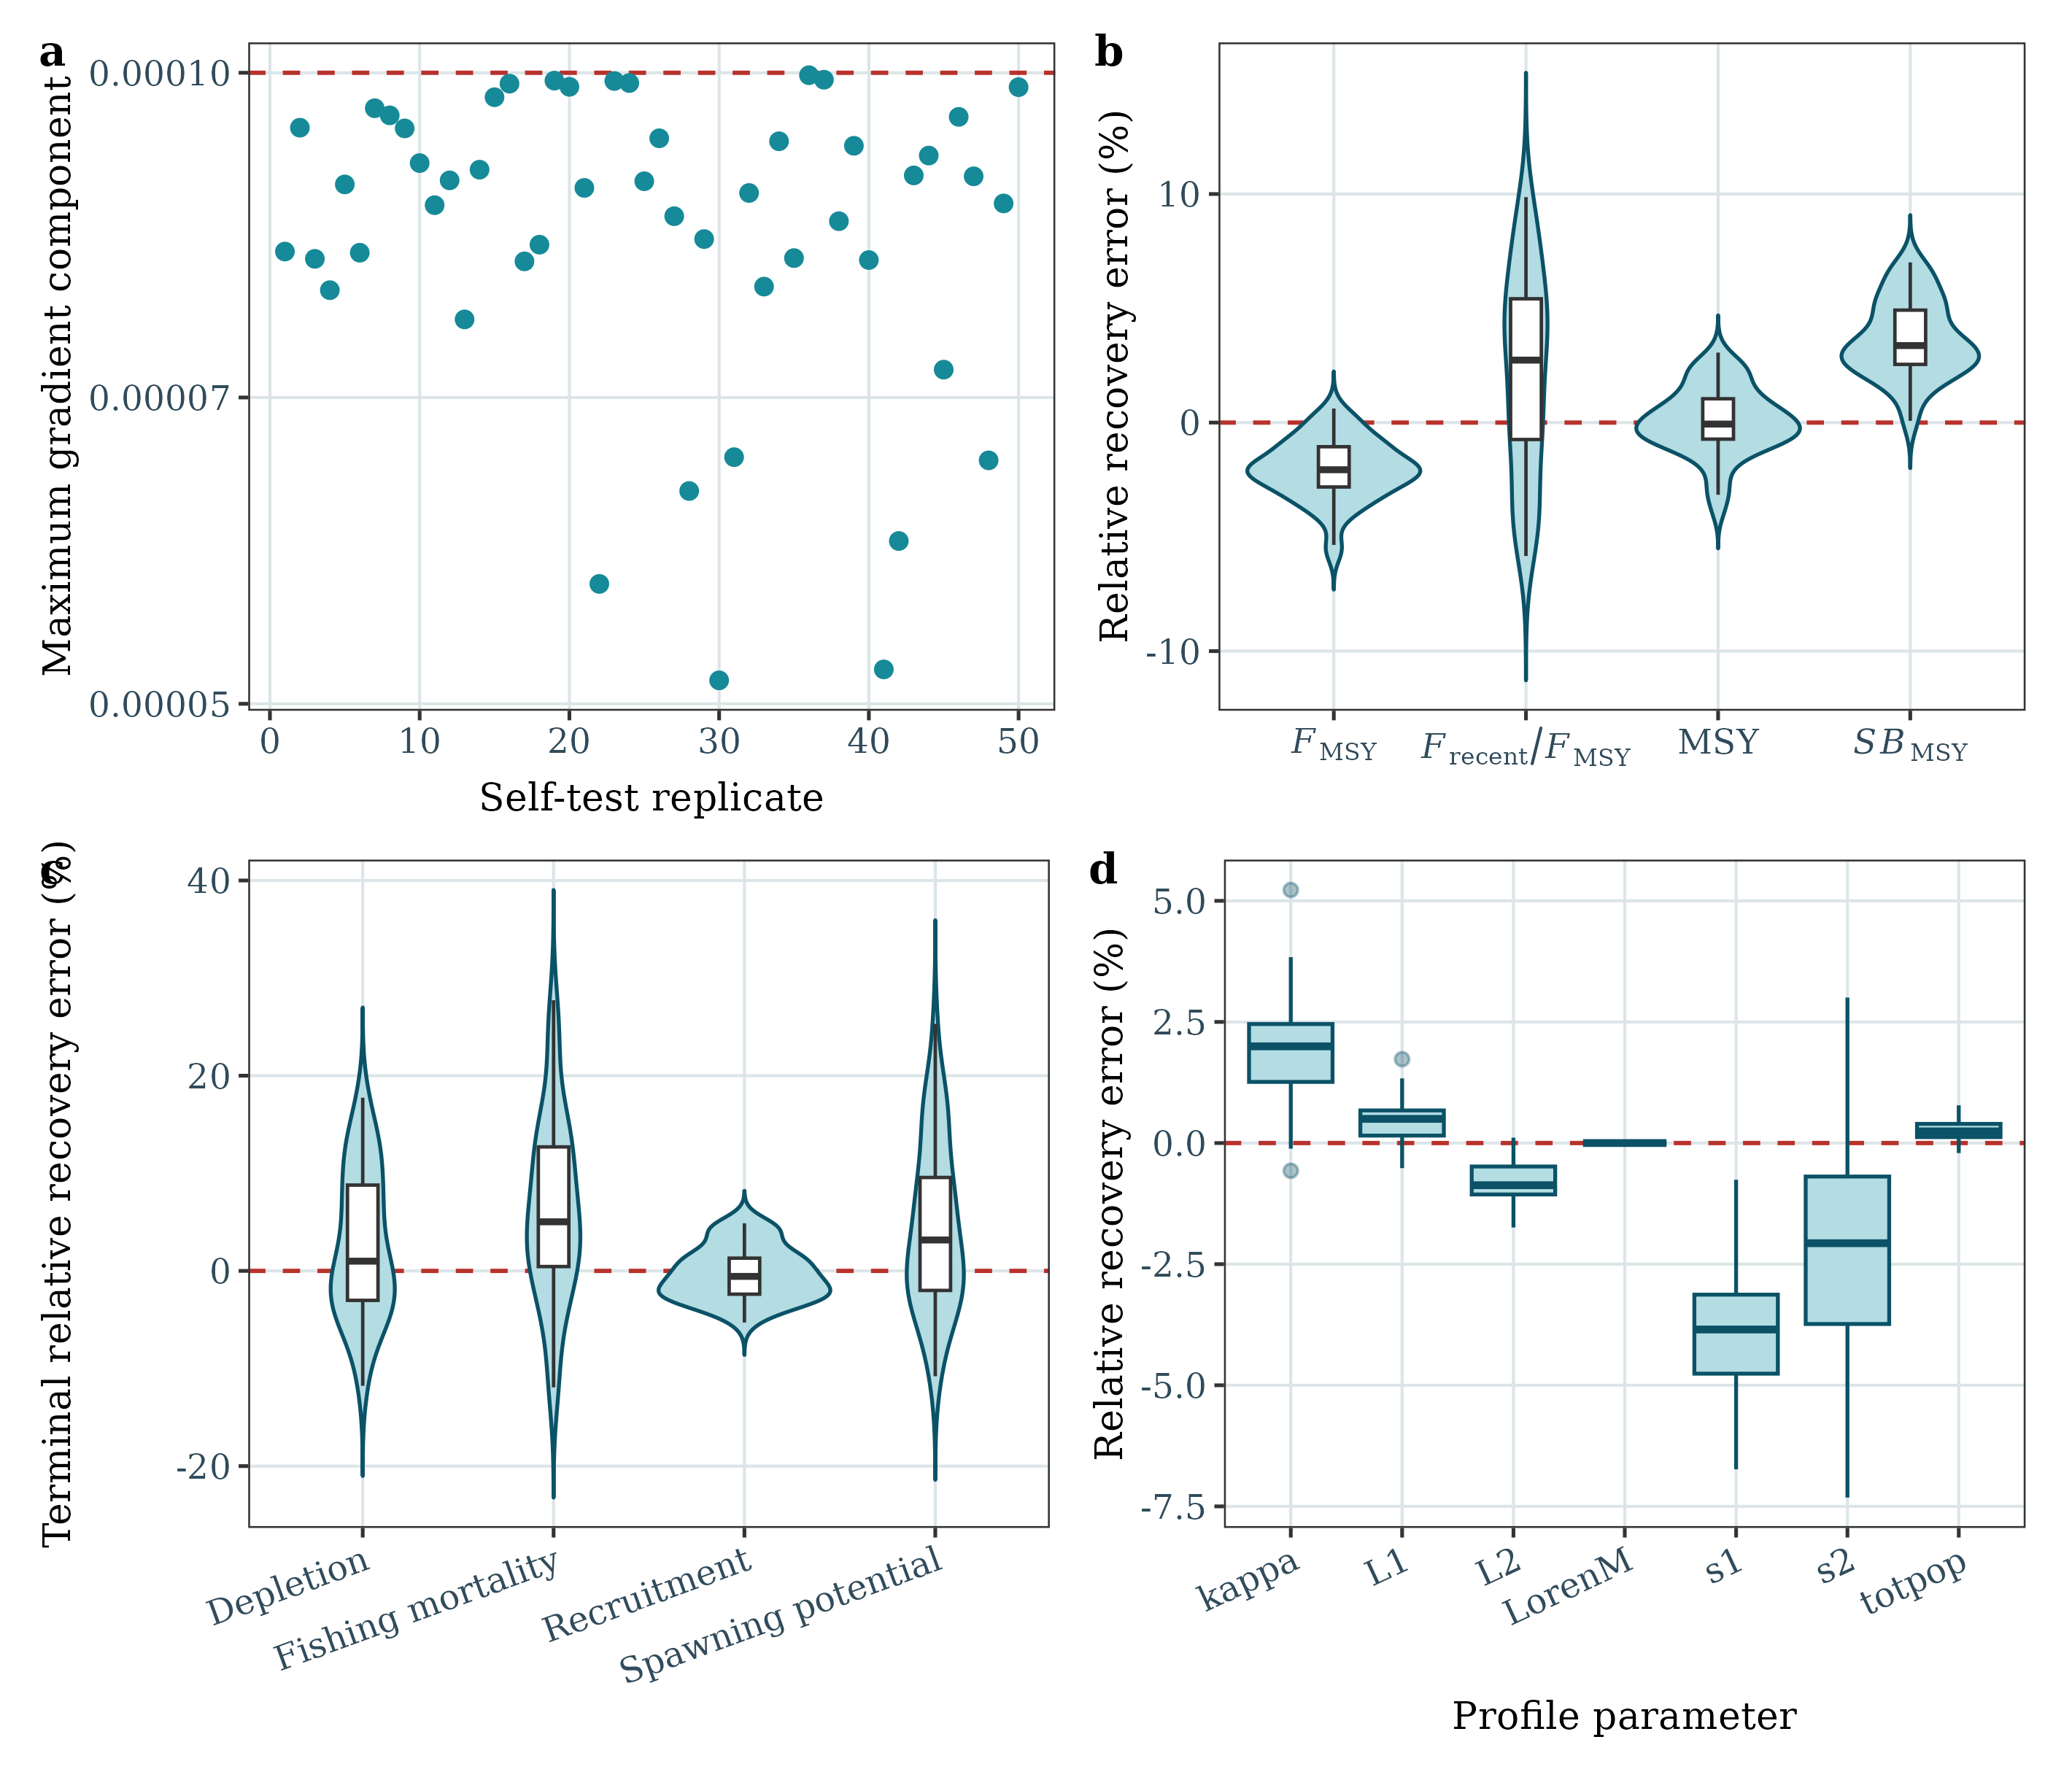
\includegraphics[width=1\linewidth,height=\textheight,keepaspectratio]{figures_new/self-test-diagnostics.png}

}

\caption{\label{fig-selftest-diagnostics}\label{fig-selftest-recovery}\label{fig-selftest-time-series}Self-test results from 50
simulated-and-refitted data sets: (a) maximum gradient component, (b)
recovery of management quantities, (c) terminal derived quantities and
(d) selected profile parameters. Relative errors are refitted minus
generating values, divided by generating values. Open the
\href{https://pacificcommunity.github.io/ofp-sam-bet-2026-selftest/selftest-report.html}{interactive
self-test report}.}

\end{figure}\DIFaddend %

\DIFdelbegin %DIFDELCMD < \begin{figure}[H]
%DIFDELCMD <

%DIFDELCMD < \centering{
%DIFDELCMD <

%DIFDELCMD < 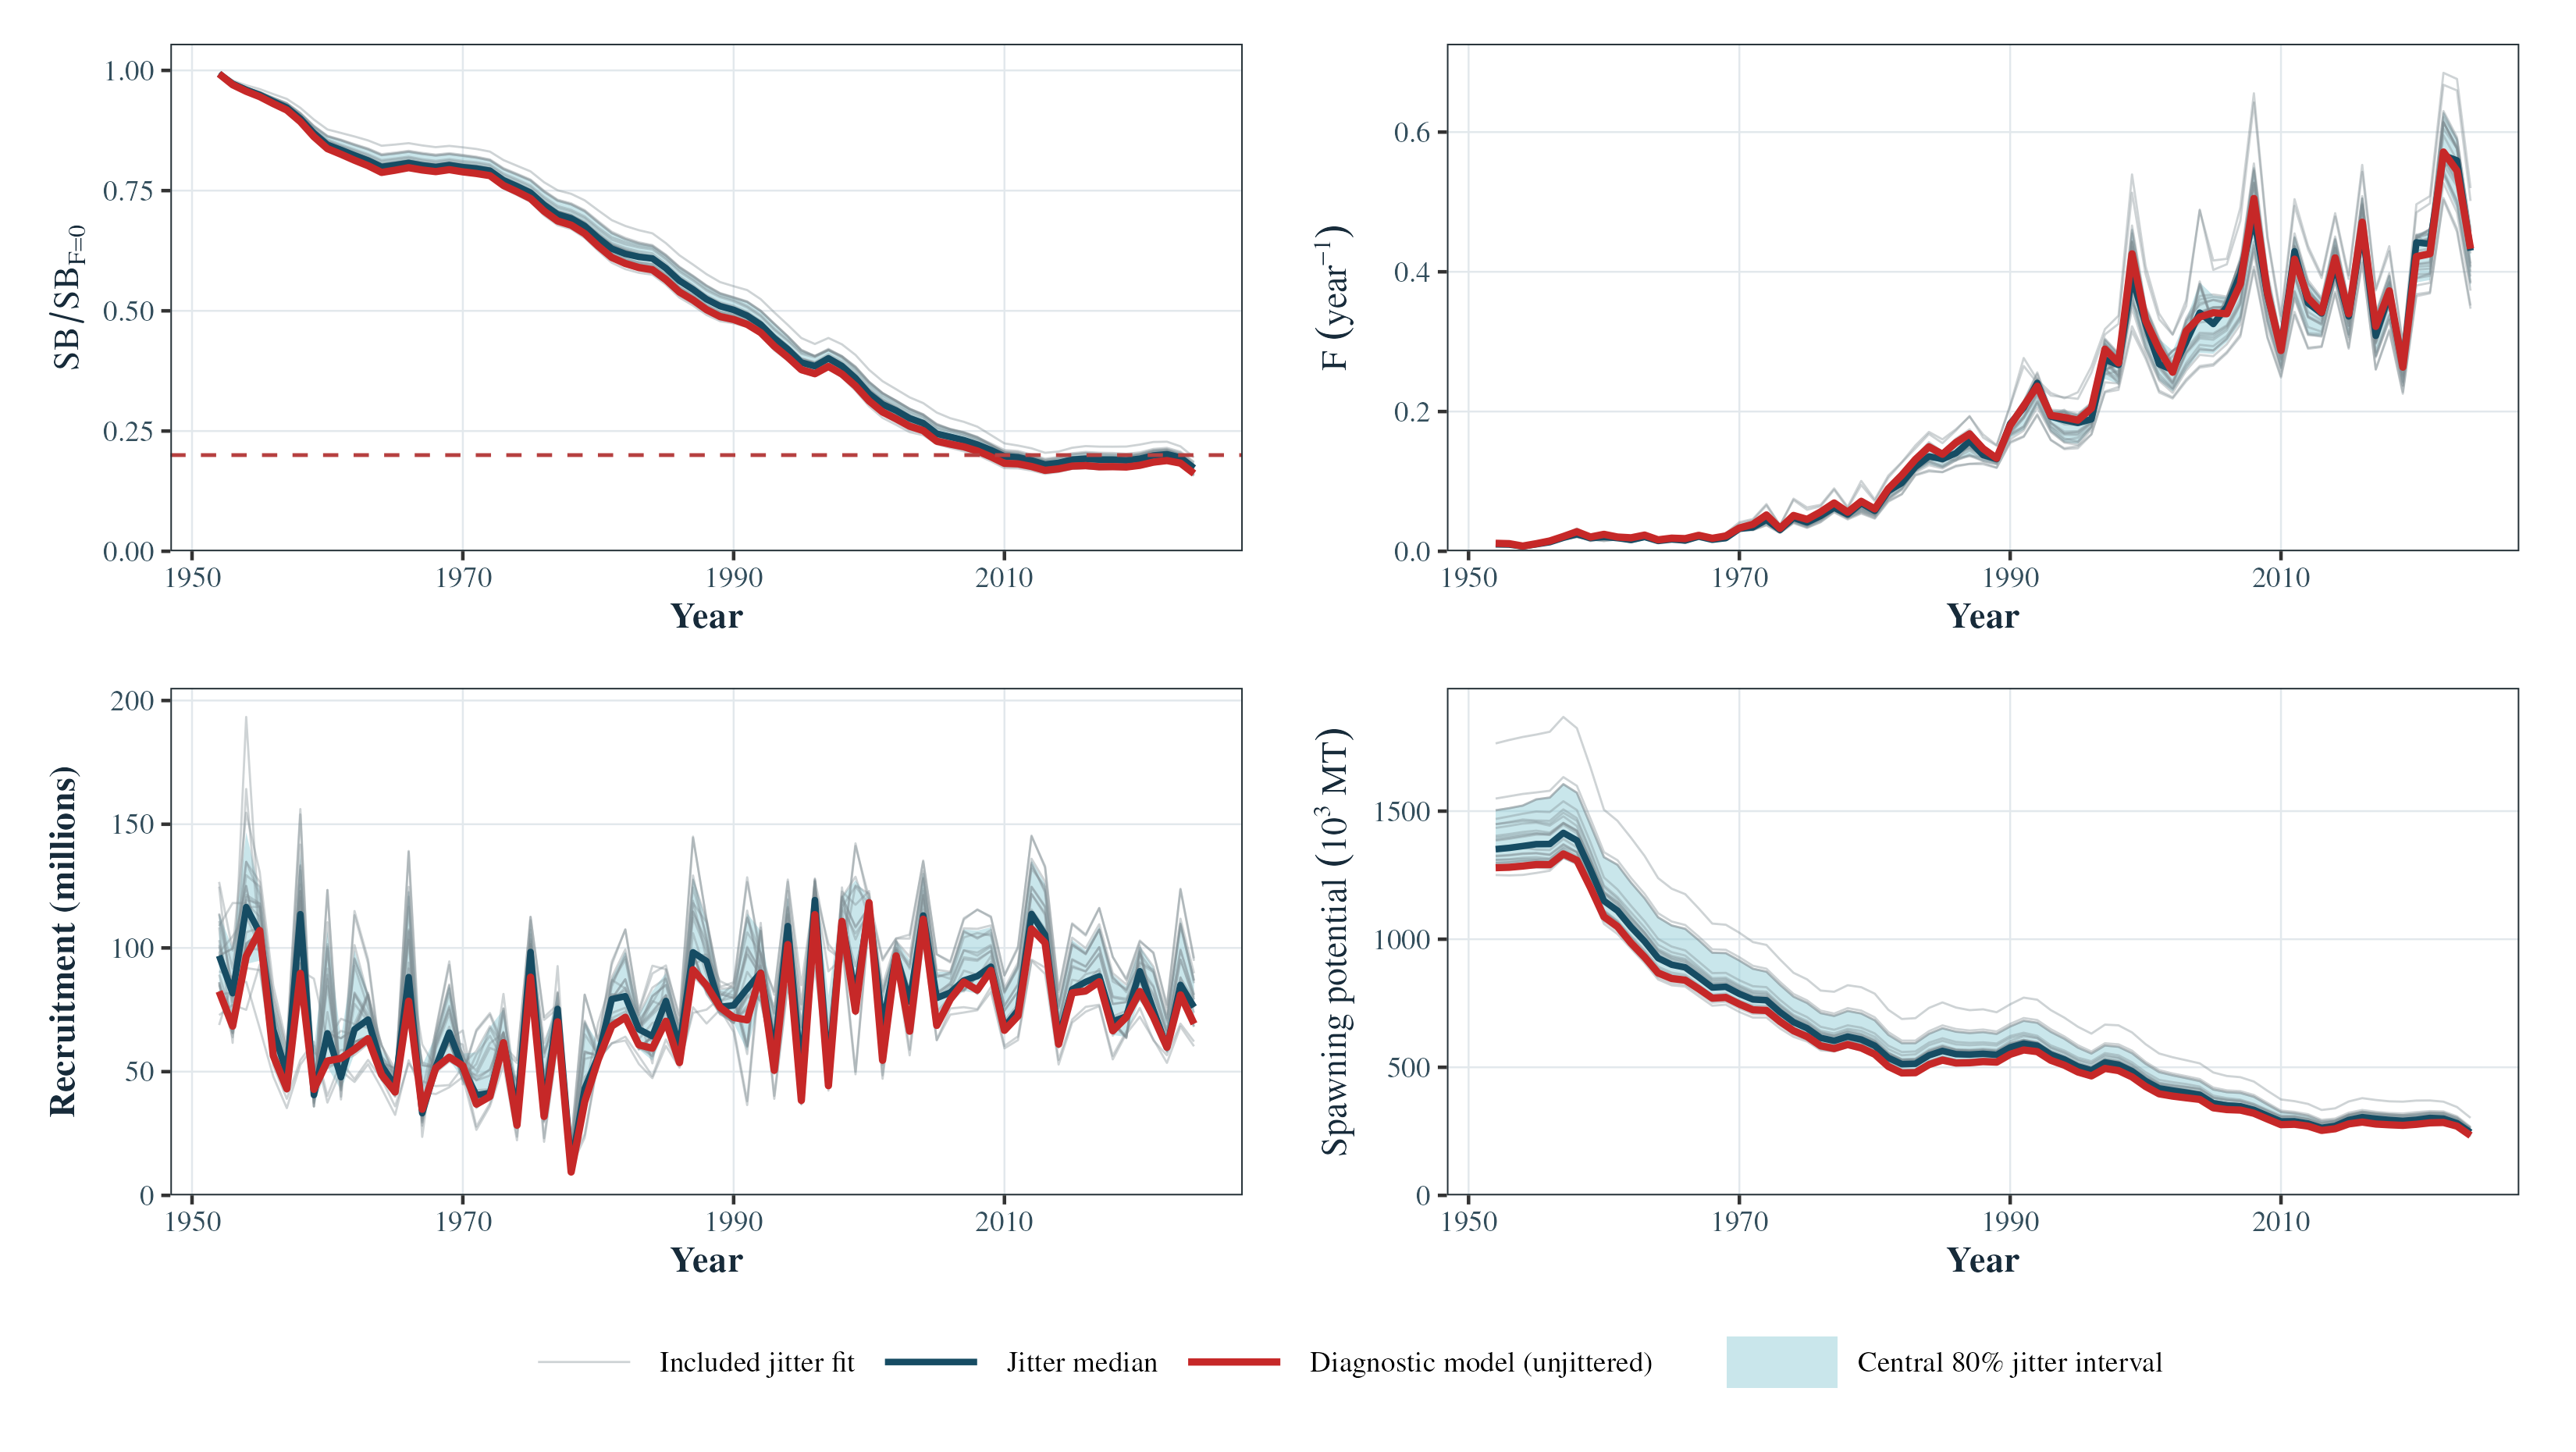
\includegraphics[width=1\linewidth,height=\textheight,keepaspectratio]{figures/jitter_derived_values_diag_panel.png}
%DIFDELCMD <

%DIFDELCMD < }
%DIFDELCMD <

%DIFDELCMD < \caption{\label{fig-jitter-derived-values-diag-panel}Annual derived
%DIFDELCMD < quantities across the 25 retained jitter fits. Thin grey-blue lines are
%DIFDELCMD < individual fits, the shaded band is the pointwise central 80\% interval
%DIFDELCMD < (10th--90th percentiles), the dark line is the jitter median, and the
%DIFDELCMD < red line is the Diagnostic model without jitter. Depletion
%DIFDELCMD < (\(SB\)/\(SB_{F=0}\)); fishing mortality is the annual instantaneous
%DIFDELCMD < rate; recruitment is in millions of fish; and spawning potential
%DIFDELCMD < (\(SB\)) in mt.}
%DIFDELCMD <

%DIFDELCMD < \end{figure}%%%
\DIFdelend \DIFaddbegin \begin{figure}[H]

\centering{

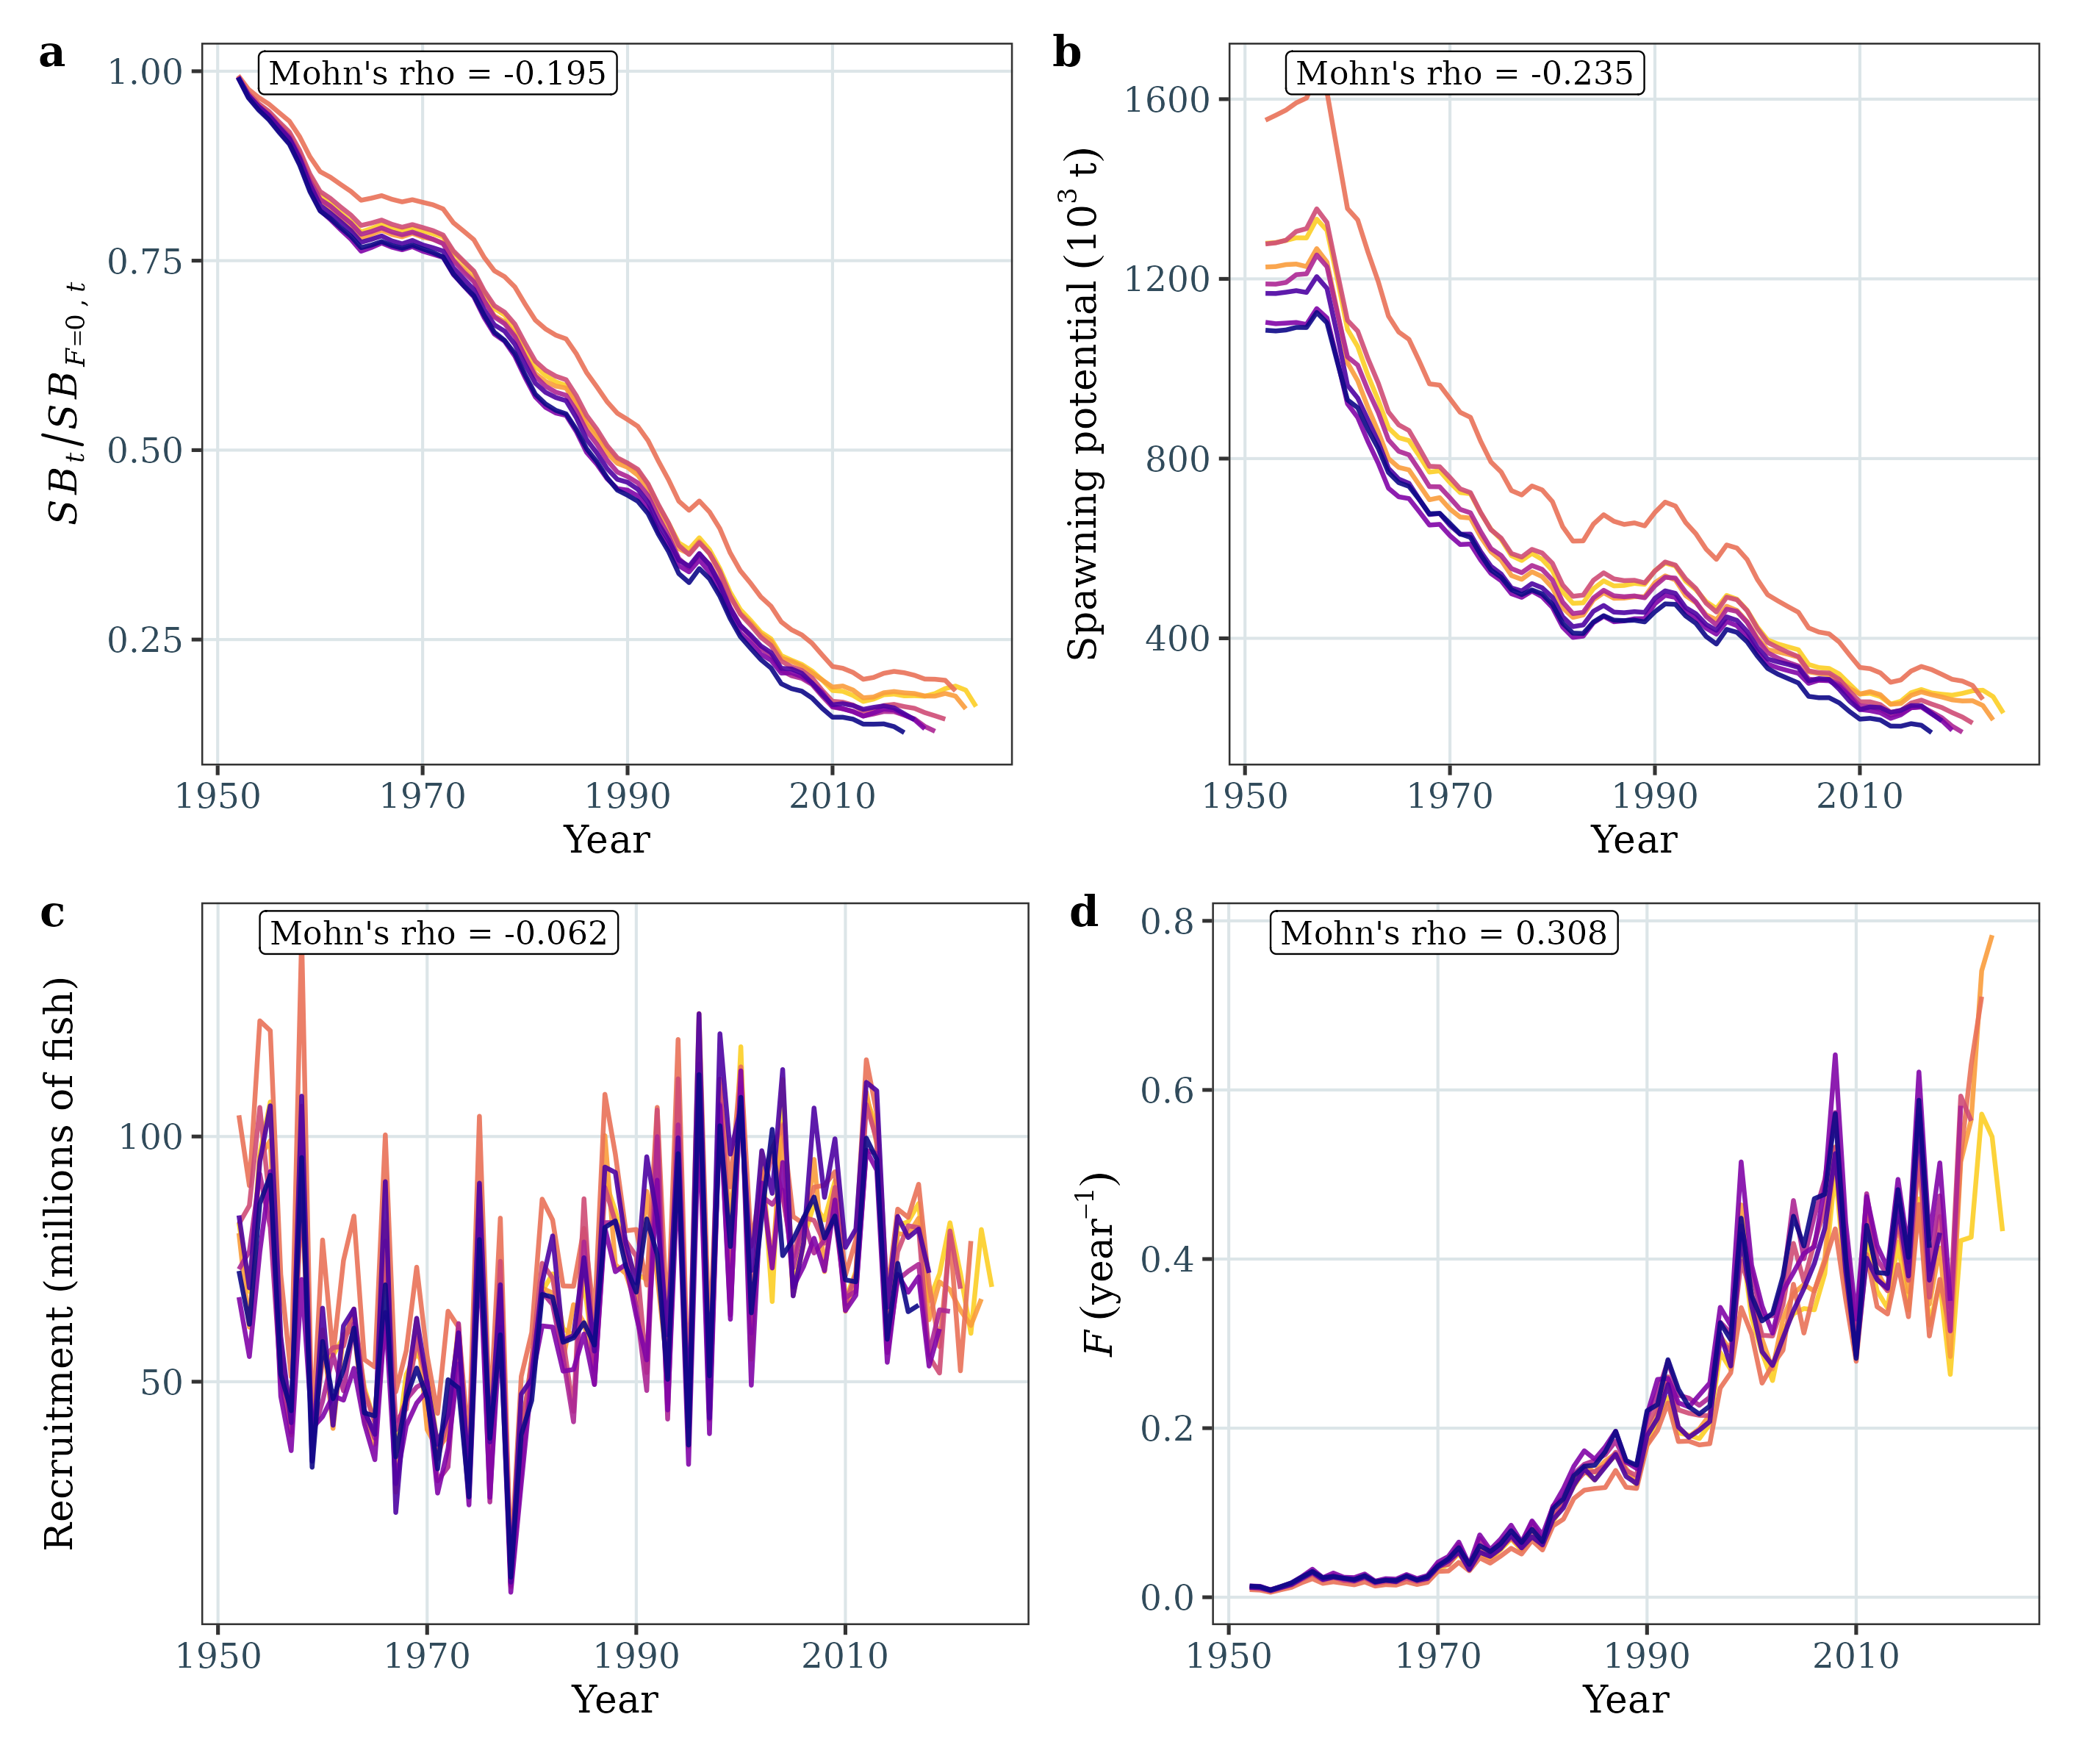
\includegraphics[width=1\linewidth,height=\textheight,keepaspectratio]{figures_new/retrospective-diagnostics.png}

}

\caption{\label{fig-retro-analysis}Retrospective trajectories for (a)
dynamic spawning depletion, (b) spawning potential, (c) recruitment and
(d) annual population-weighted fishing mortality. Colours distinguish
the diagnostic fit and seven terminal-year peels; labels give Mohn's
\(\rho\). Open the
\href{https://pacificcommunity.github.io/ofp-sam-bet-2026-retrospective/retrospective-report.html}{interactive
retrospective report}.}

\end{figure}\DIFaddend %

\DIFdelbegin %DIFDELCMD < \begin{figure}[H]
%DIFDELCMD <

%DIFDELCMD < \centering{
%DIFDELCMD <

%DIFDELCMD < 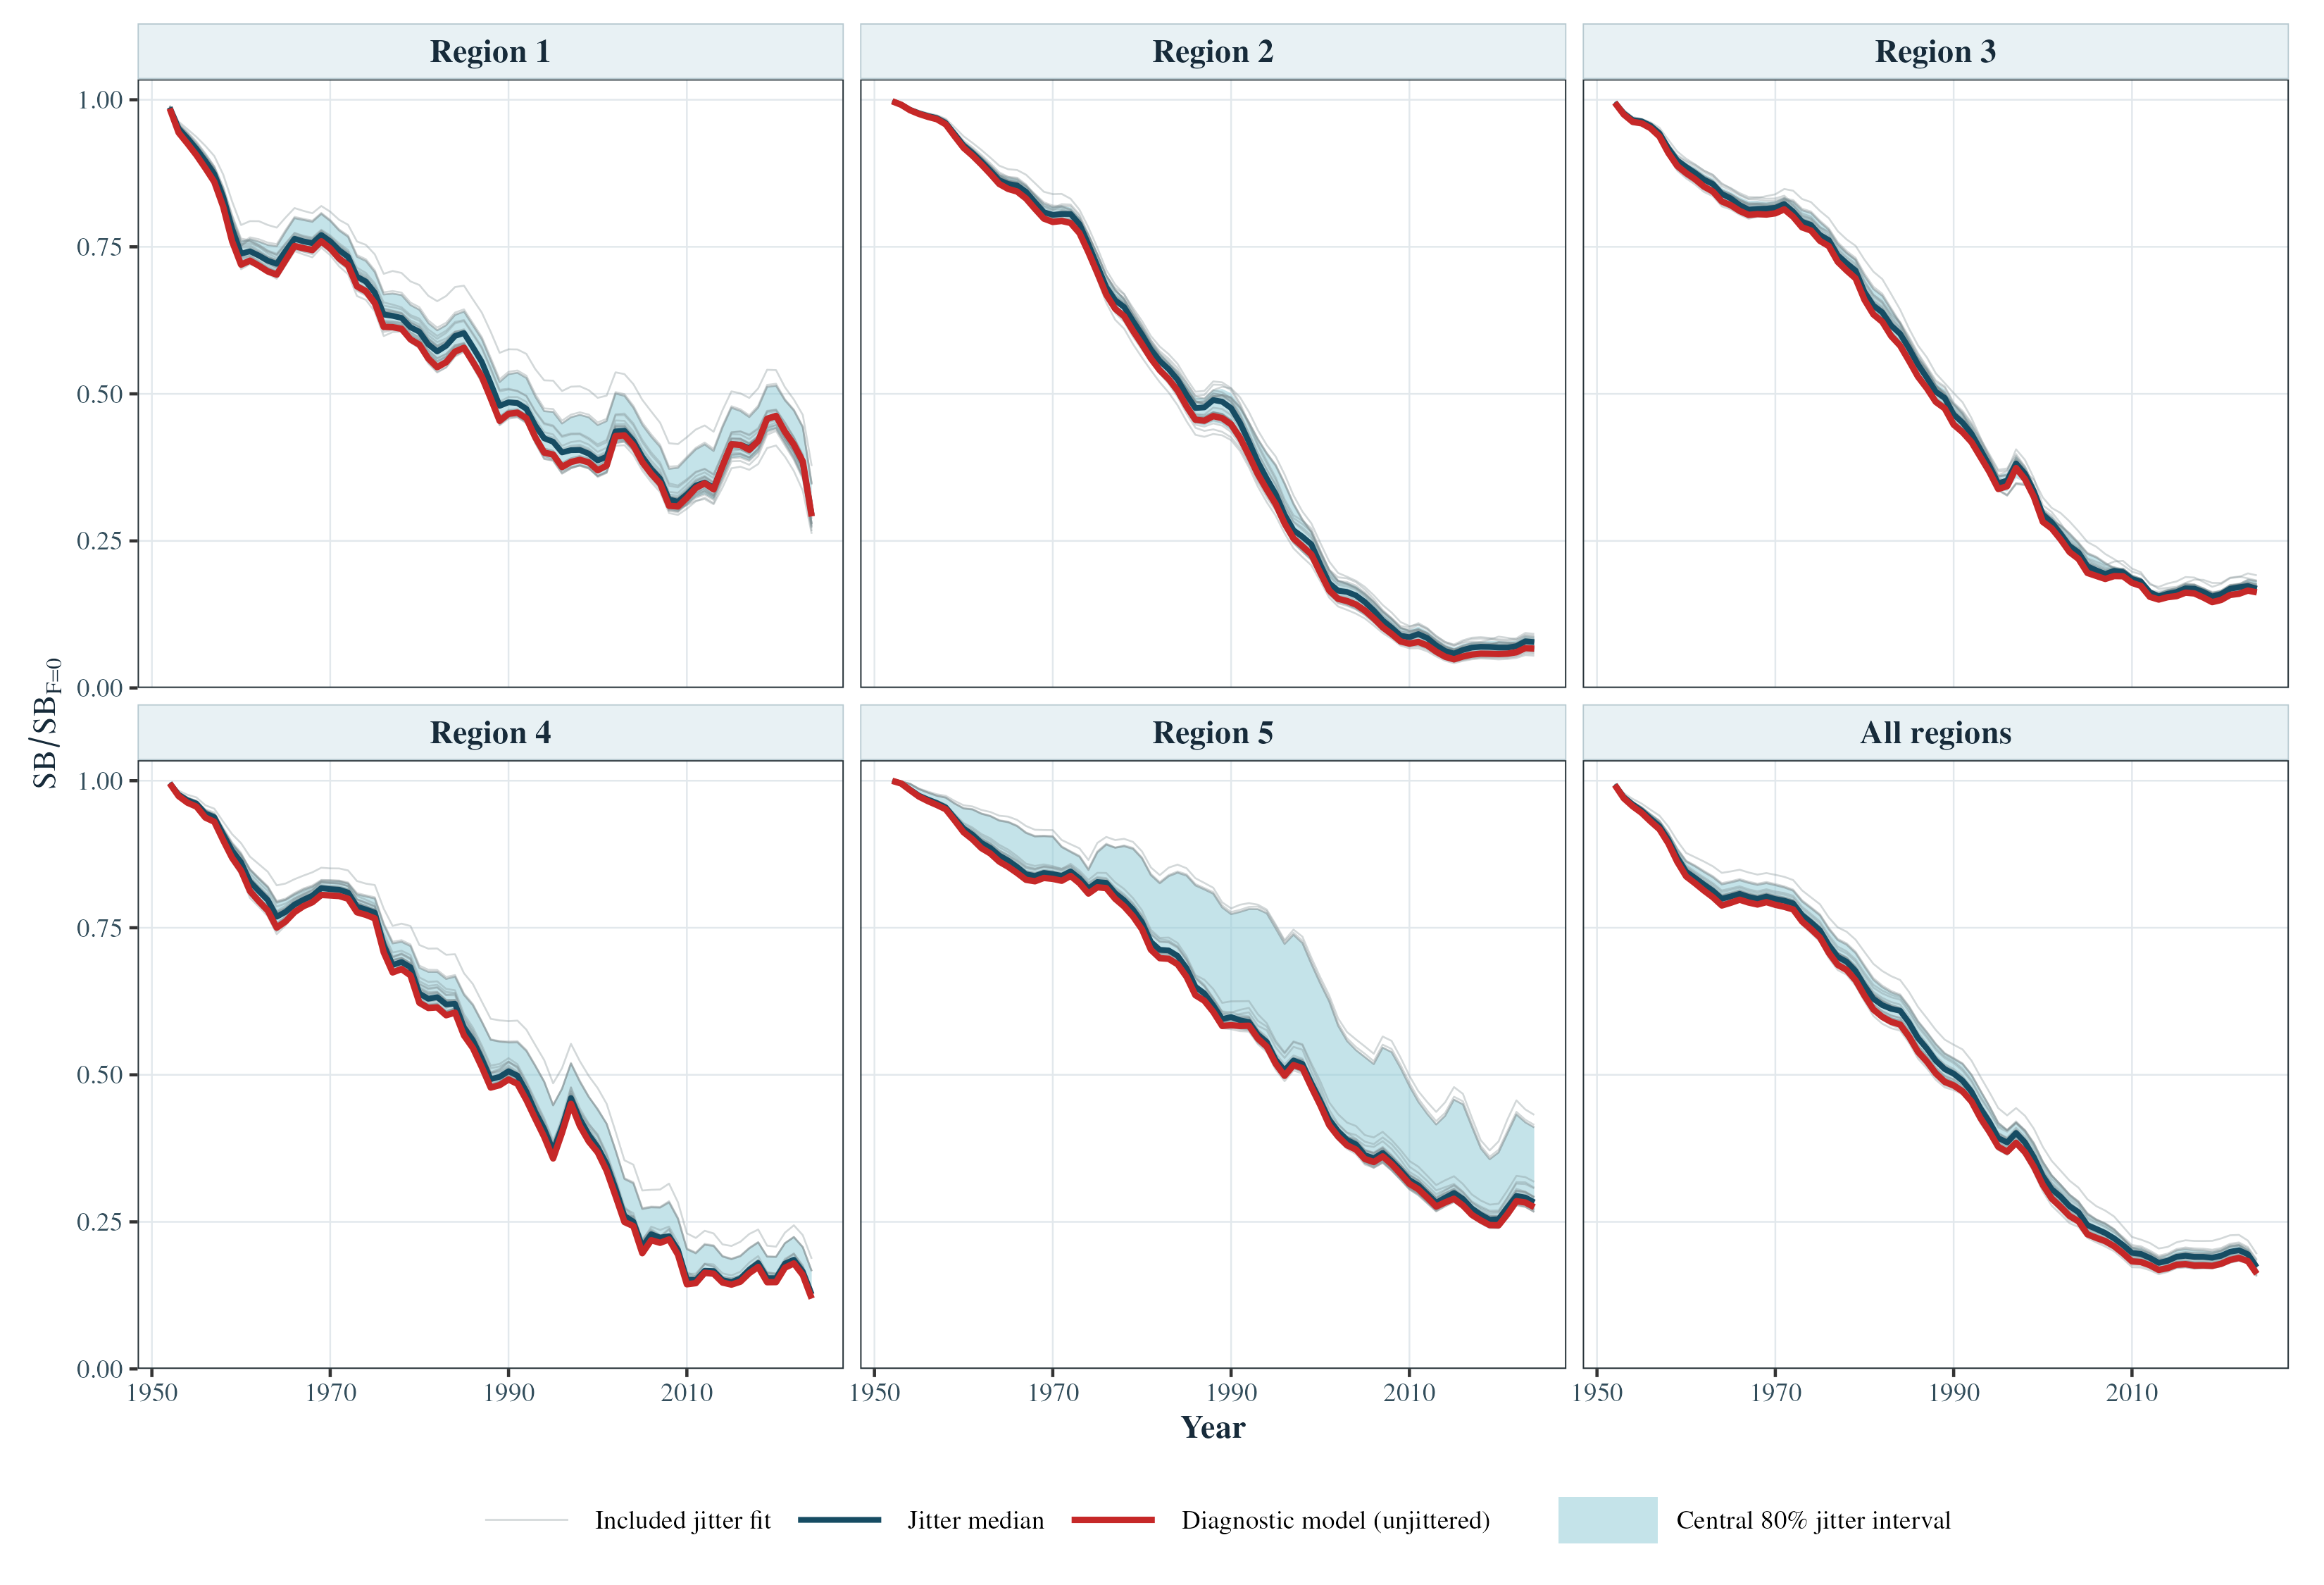
\includegraphics[width=1\linewidth,height=\textheight,keepaspectratio]{figures/jitter_regional_depletion.png}
%DIFDELCMD <

%DIFDELCMD < }
%DIFDELCMD <

%DIFDELCMD < \caption{\label{fig-jitter-regional-depletion}Annual derived quantities
%DIFDELCMD < across the 25 retained jitter fits are shown by model region for
%DIFDELCMD < depletion (\(SB\)/\(SB_{F=0}\)). Thin grey-blue lines are individual
%DIFDELCMD < fits, the shaded band is the pointwise central 80\% interval (10th--90th
%DIFDELCMD < percentiles), the dark line is the jitter median, and the red line is
%DIFDELCMD < the Diagnostic model without jitter.}
%DIFDELCMD <

%DIFDELCMD < \end{figure}%%%
\DIFdelend \DIFaddbegin \begin{figure}[H]

\centering{

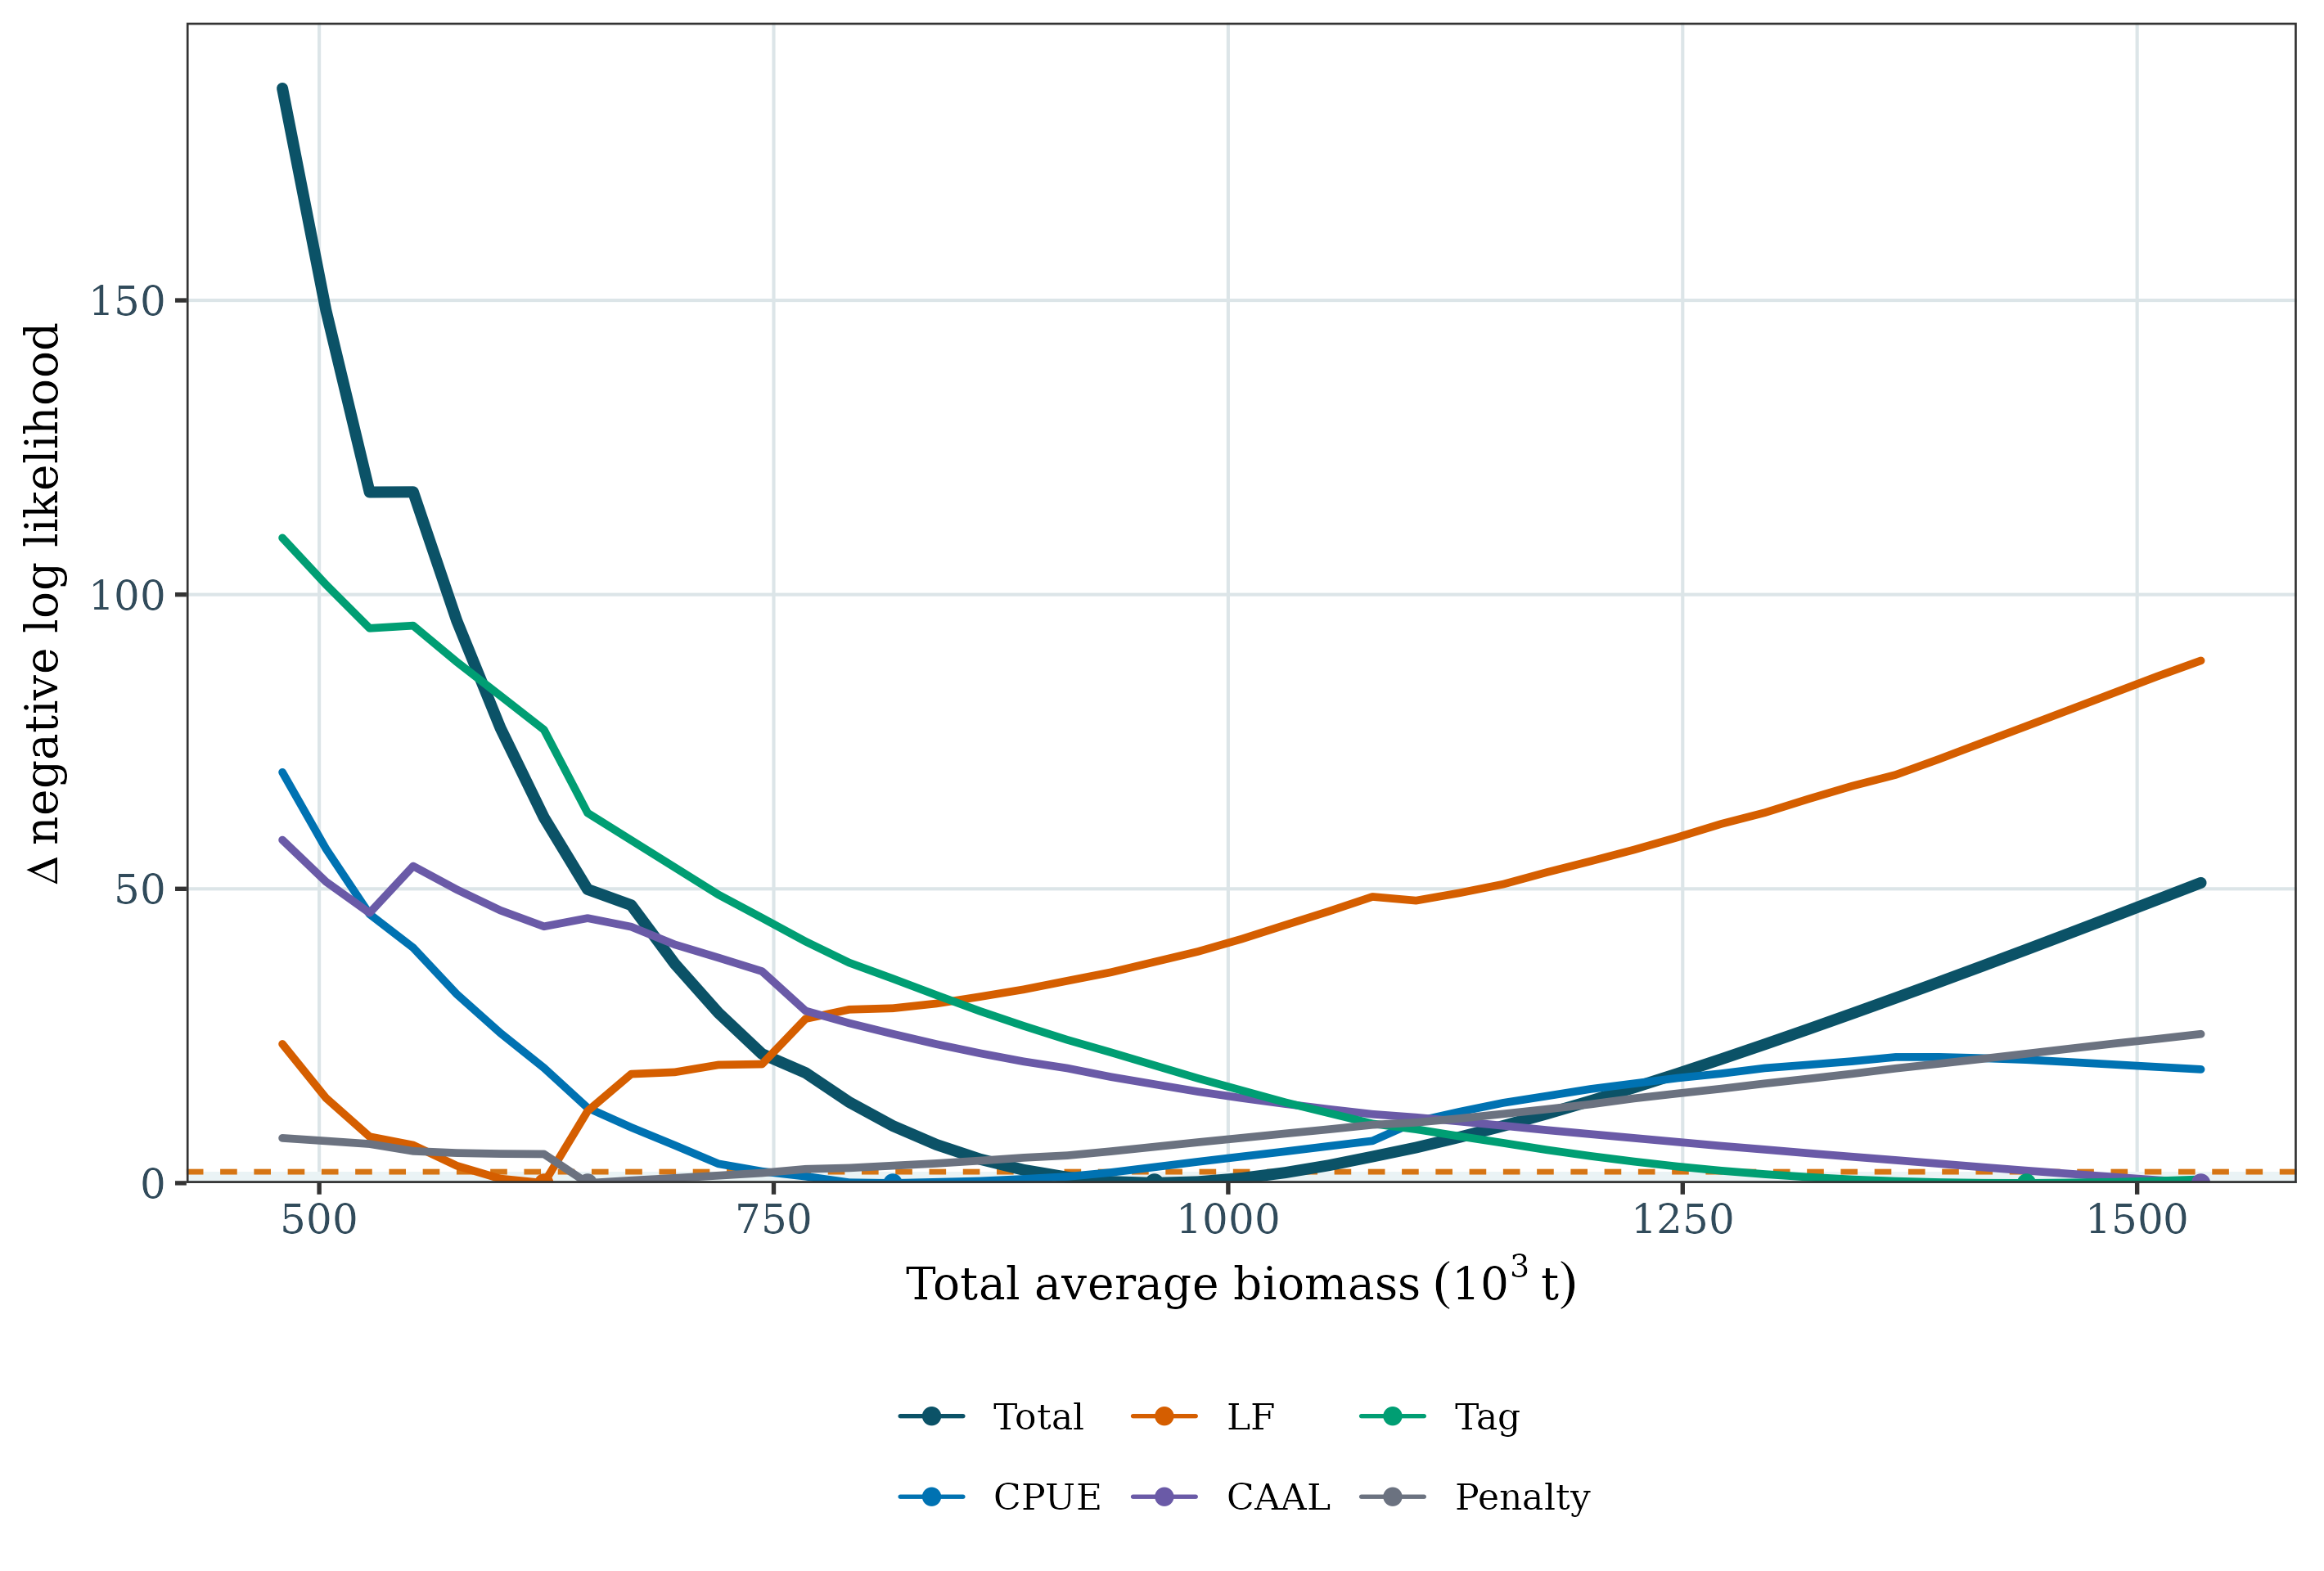
\includegraphics[width=1\linewidth,height=\textheight,keepaspectratio]{figures_new/likelihood-profile-components.png}

}

\caption{\label{fig-diag-profile-data-sources}Overall-objective and
component likelihood profiles overlaid on the absolute
total-average-biomass scale. Each curve is expressed as a change from
its own minimum; the horizontal line marks a change of 1.92. Open the
\href{https://pacificcommunity.github.io/ofp-sam-bet-2026-diagnostic/bet-2026-likelihood-profile-viewer.html}{interactive
profile viewer}.}

\end{figure}\DIFaddend %

\DIFdelbegin %DIFDELCMD < \begin{figure}[H]
%DIFDELCMD <

%DIFDELCMD < \centering{
%DIFDELCMD <

%DIFDELCMD < 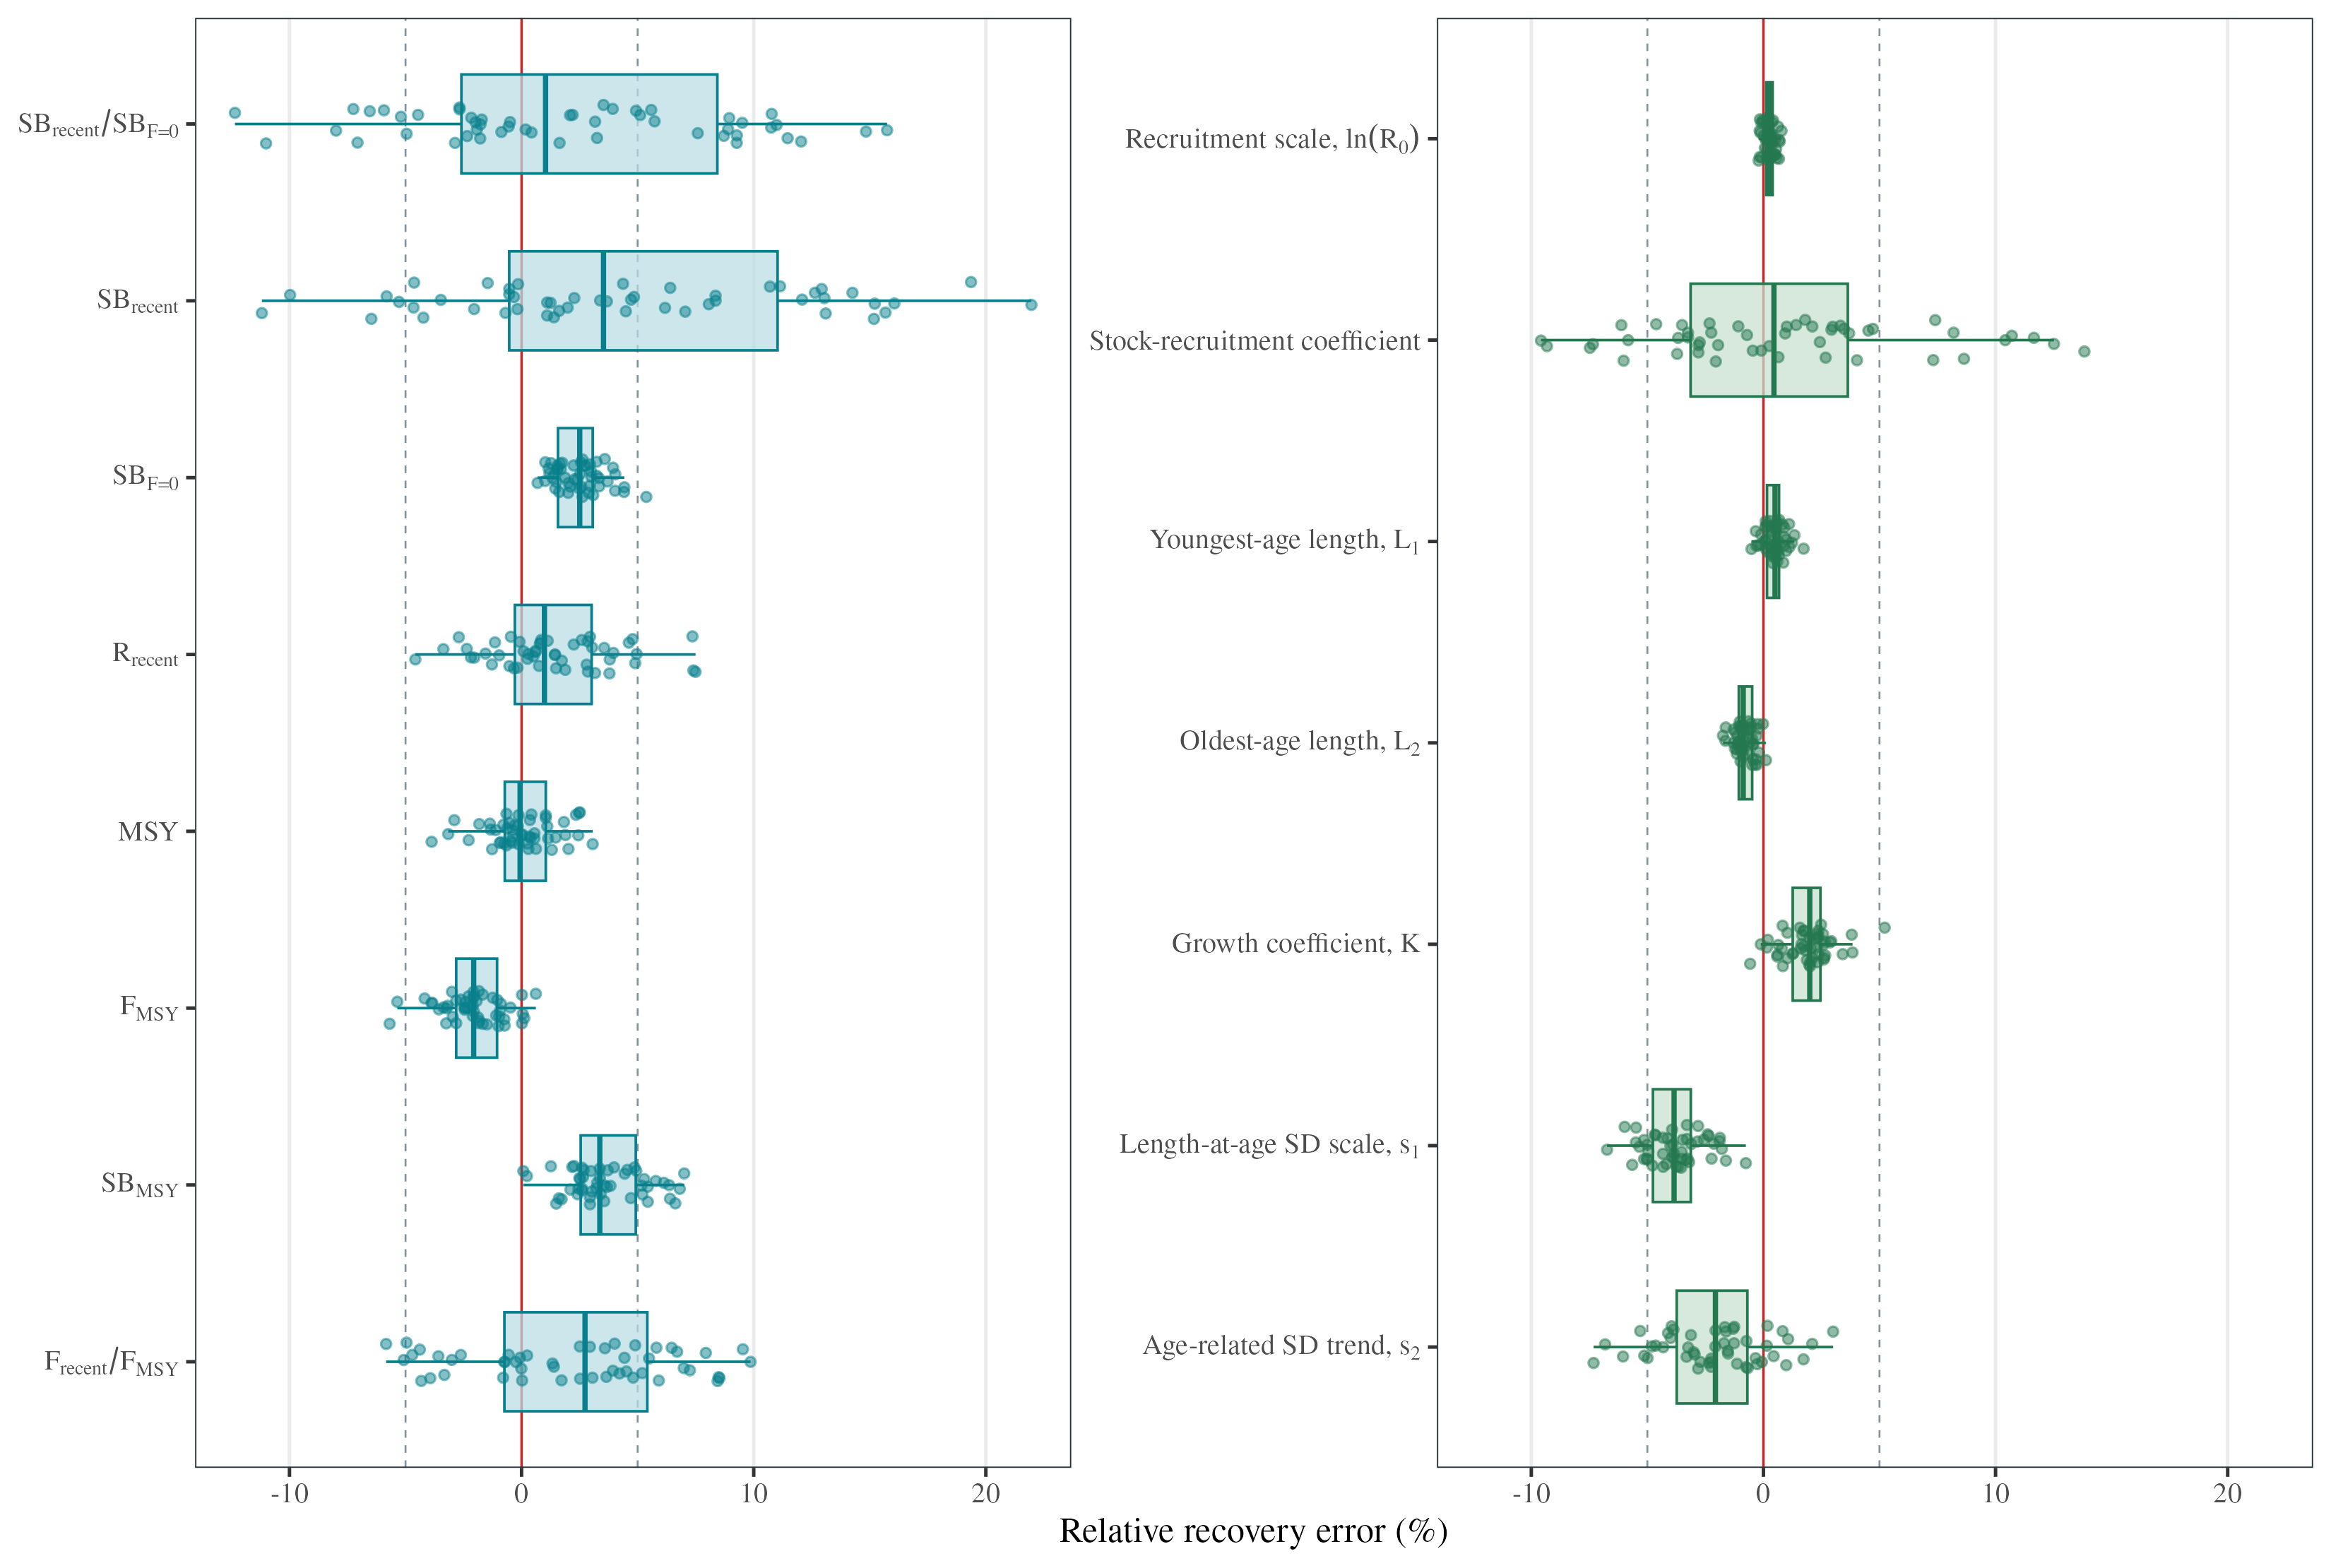
\includegraphics[width=1\linewidth,height=\textheight,keepaspectratio]{figures/selftest_recovery_diag.png}
%DIFDELCMD <

%DIFDELCMD < }
%DIFDELCMD <

%DIFDELCMD < \caption{\label{fig-selftest-recovery}Relative recovery error for recent
%DIFDELCMD < management and assessment quantities ending in 2024 and for selected
%DIFDELCMD < estimated parameters in the Diagnostic model. The left panel includes
%DIFDELCMD < recent depletion, recent and unfished spawning potential, recent
%DIFDELCMD < recruitment, MSY, fishing mortality and equilibrium spawning biomass at
%DIFDELCMD < MSY, and recent fishing mortality relative to MSY. Points are
%DIFDELCMD < pseudo-data refits, boxes show their empirical distributions, and the
%DIFDELCMD < red line marks exact recovery. Grey dashed lines mark relative recovery
%DIFDELCMD < errors of -5\% and +5\%.}
%DIFDELCMD <

%DIFDELCMD < \end{figure}%%%
\DIFdelend \DIFaddbegin \begin{figure}[H]

\centering{

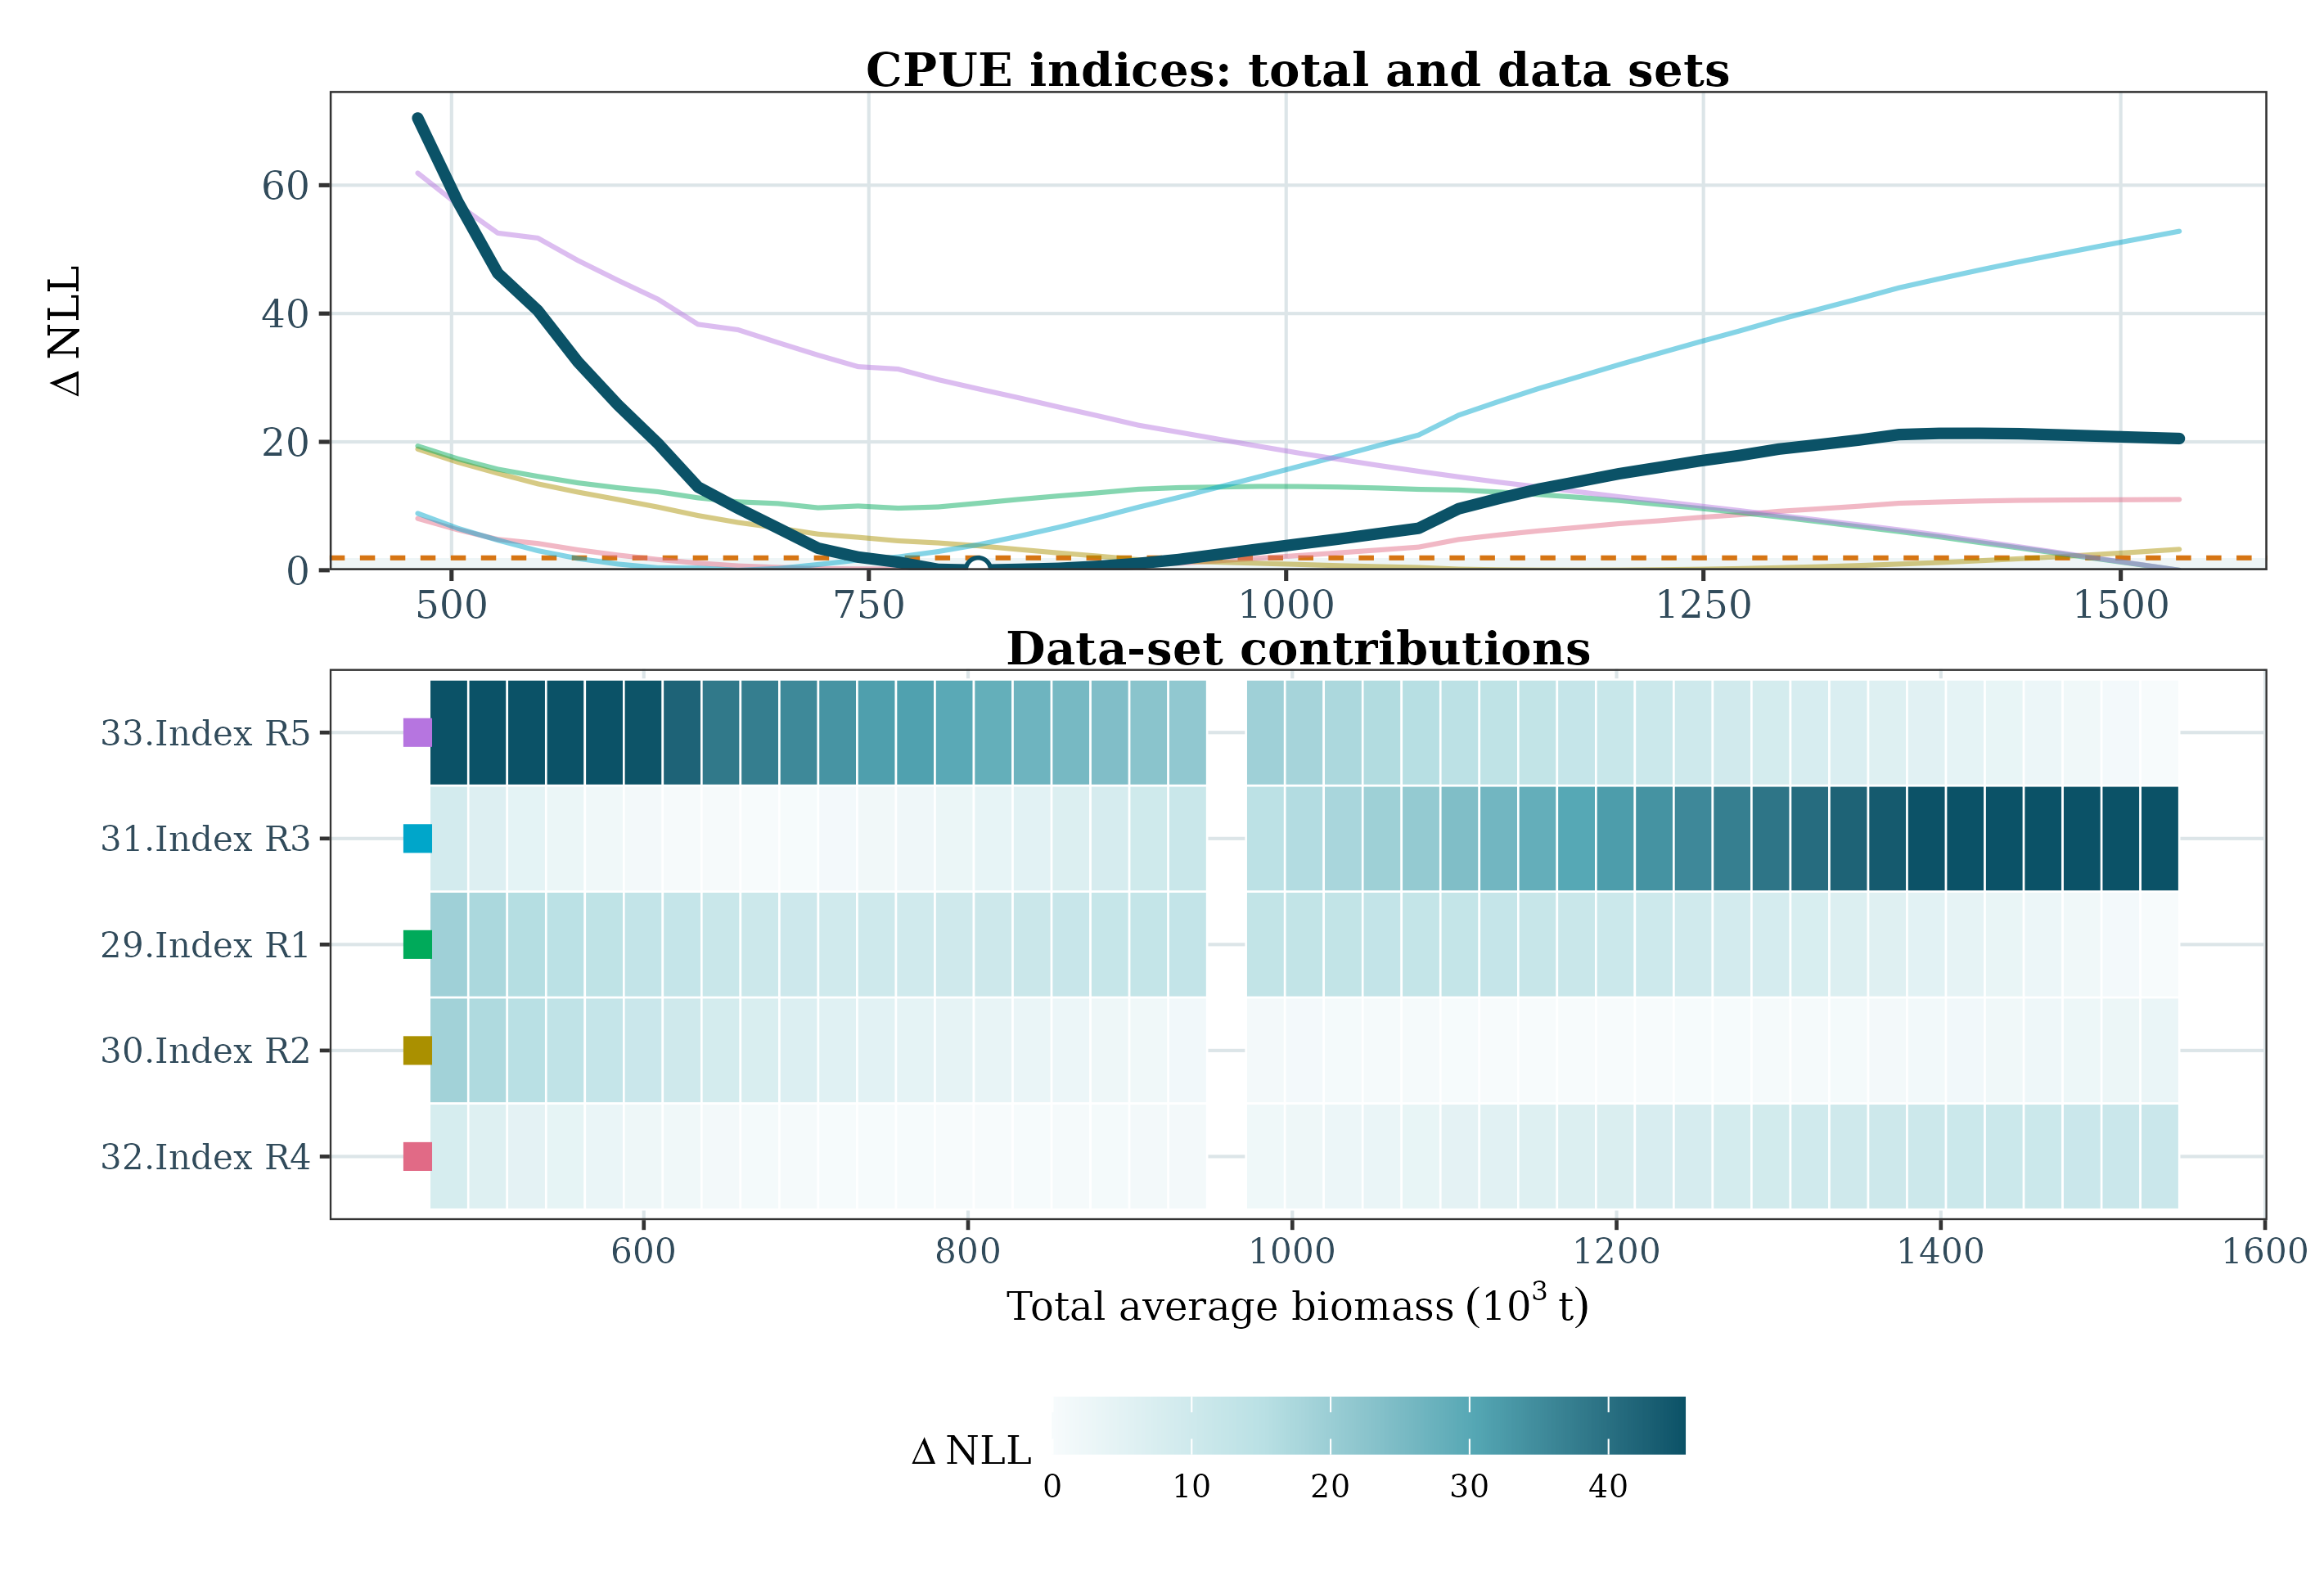
\includegraphics[width=1\linewidth,height=\textheight,keepaspectratio]{figures_new/likelihood-profile-cpue-detail.png}

}

\caption{\label{fig-diag-profile-data-cpue}CPUE likelihood profile. The
upper panel overlays the prominent CPUE total with thin, muted index
curves; coloured row keys connect those curves to the five heatmap
contributions, each expressed as a change from its own minimum. Open the
\href{https://pacificcommunity.github.io/ofp-sam-bet-2026-diagnostic/bet-2026-likelihood-profile-viewer.html}{interactive
profile viewer} to select an index.}

\end{figure}\DIFaddend %

\DIFdelbegin %DIFDELCMD < \begin{figure}[H]
%DIFDELCMD <

%DIFDELCMD < \centering{
%DIFDELCMD <

%DIFDELCMD < 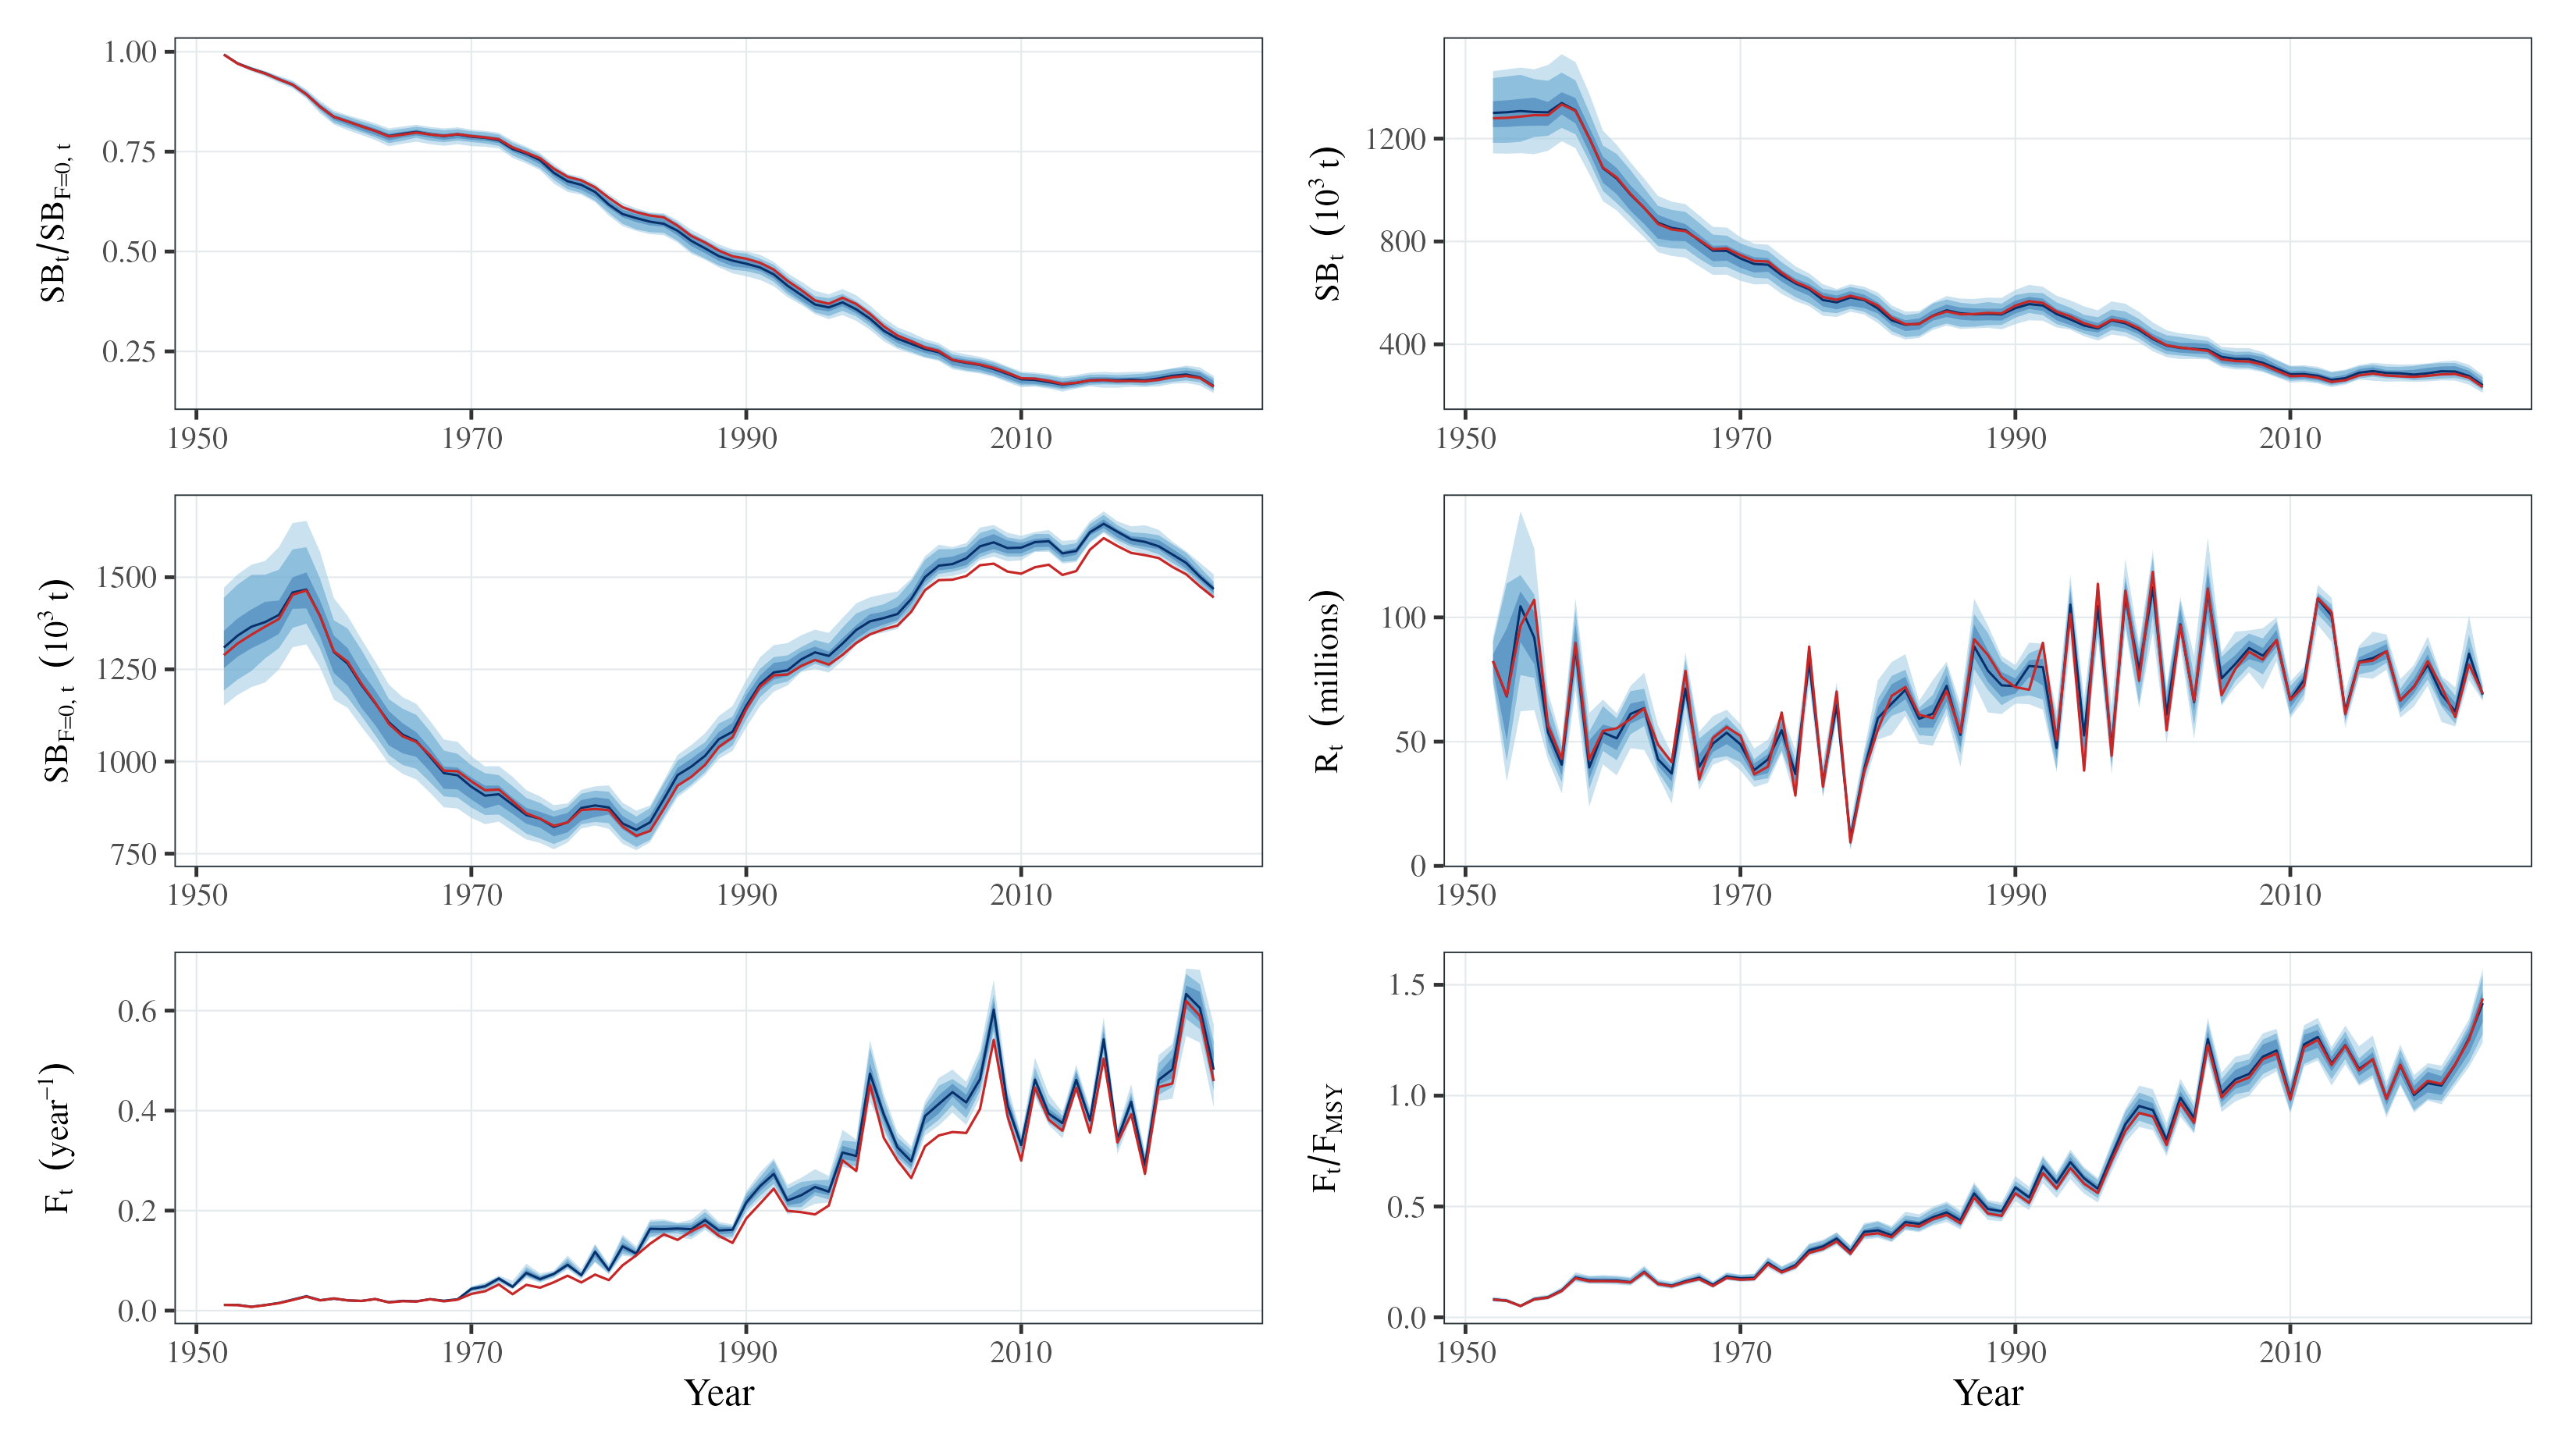
\includegraphics[width=1\linewidth,height=\textheight,keepaspectratio]{figures/selftest_time_series.png}
%DIFDELCMD <

%DIFDELCMD < }
%DIFDELCMD <

%DIFDELCMD < \caption{\label{fig-selftest-time-series}Self-test recovery of annual
%DIFDELCMD < assessment quantities for the Diagnostic model. The red line is the
%DIFDELCMD < generating truth; the dark-blue line is the median across all 50
%DIFDELCMD < replicate refits, and the nested blue bands are the central 50\%, 80\%,
%DIFDELCMD < and 95\% empirical ranges. Dynamic depletion is (\(SB\)/\(SB_{F=0}\)),
%DIFDELCMD < unfished spawning potential (\(SB_{F=0}\)), recruitment (R), fishing
%DIFDELCMD < mortality (F) and F/Fmsy.}
%DIFDELCMD <

%DIFDELCMD < \end{figure}%%%
\DIFdelend \DIFaddbegin \begin{figure}[H]

\centering{

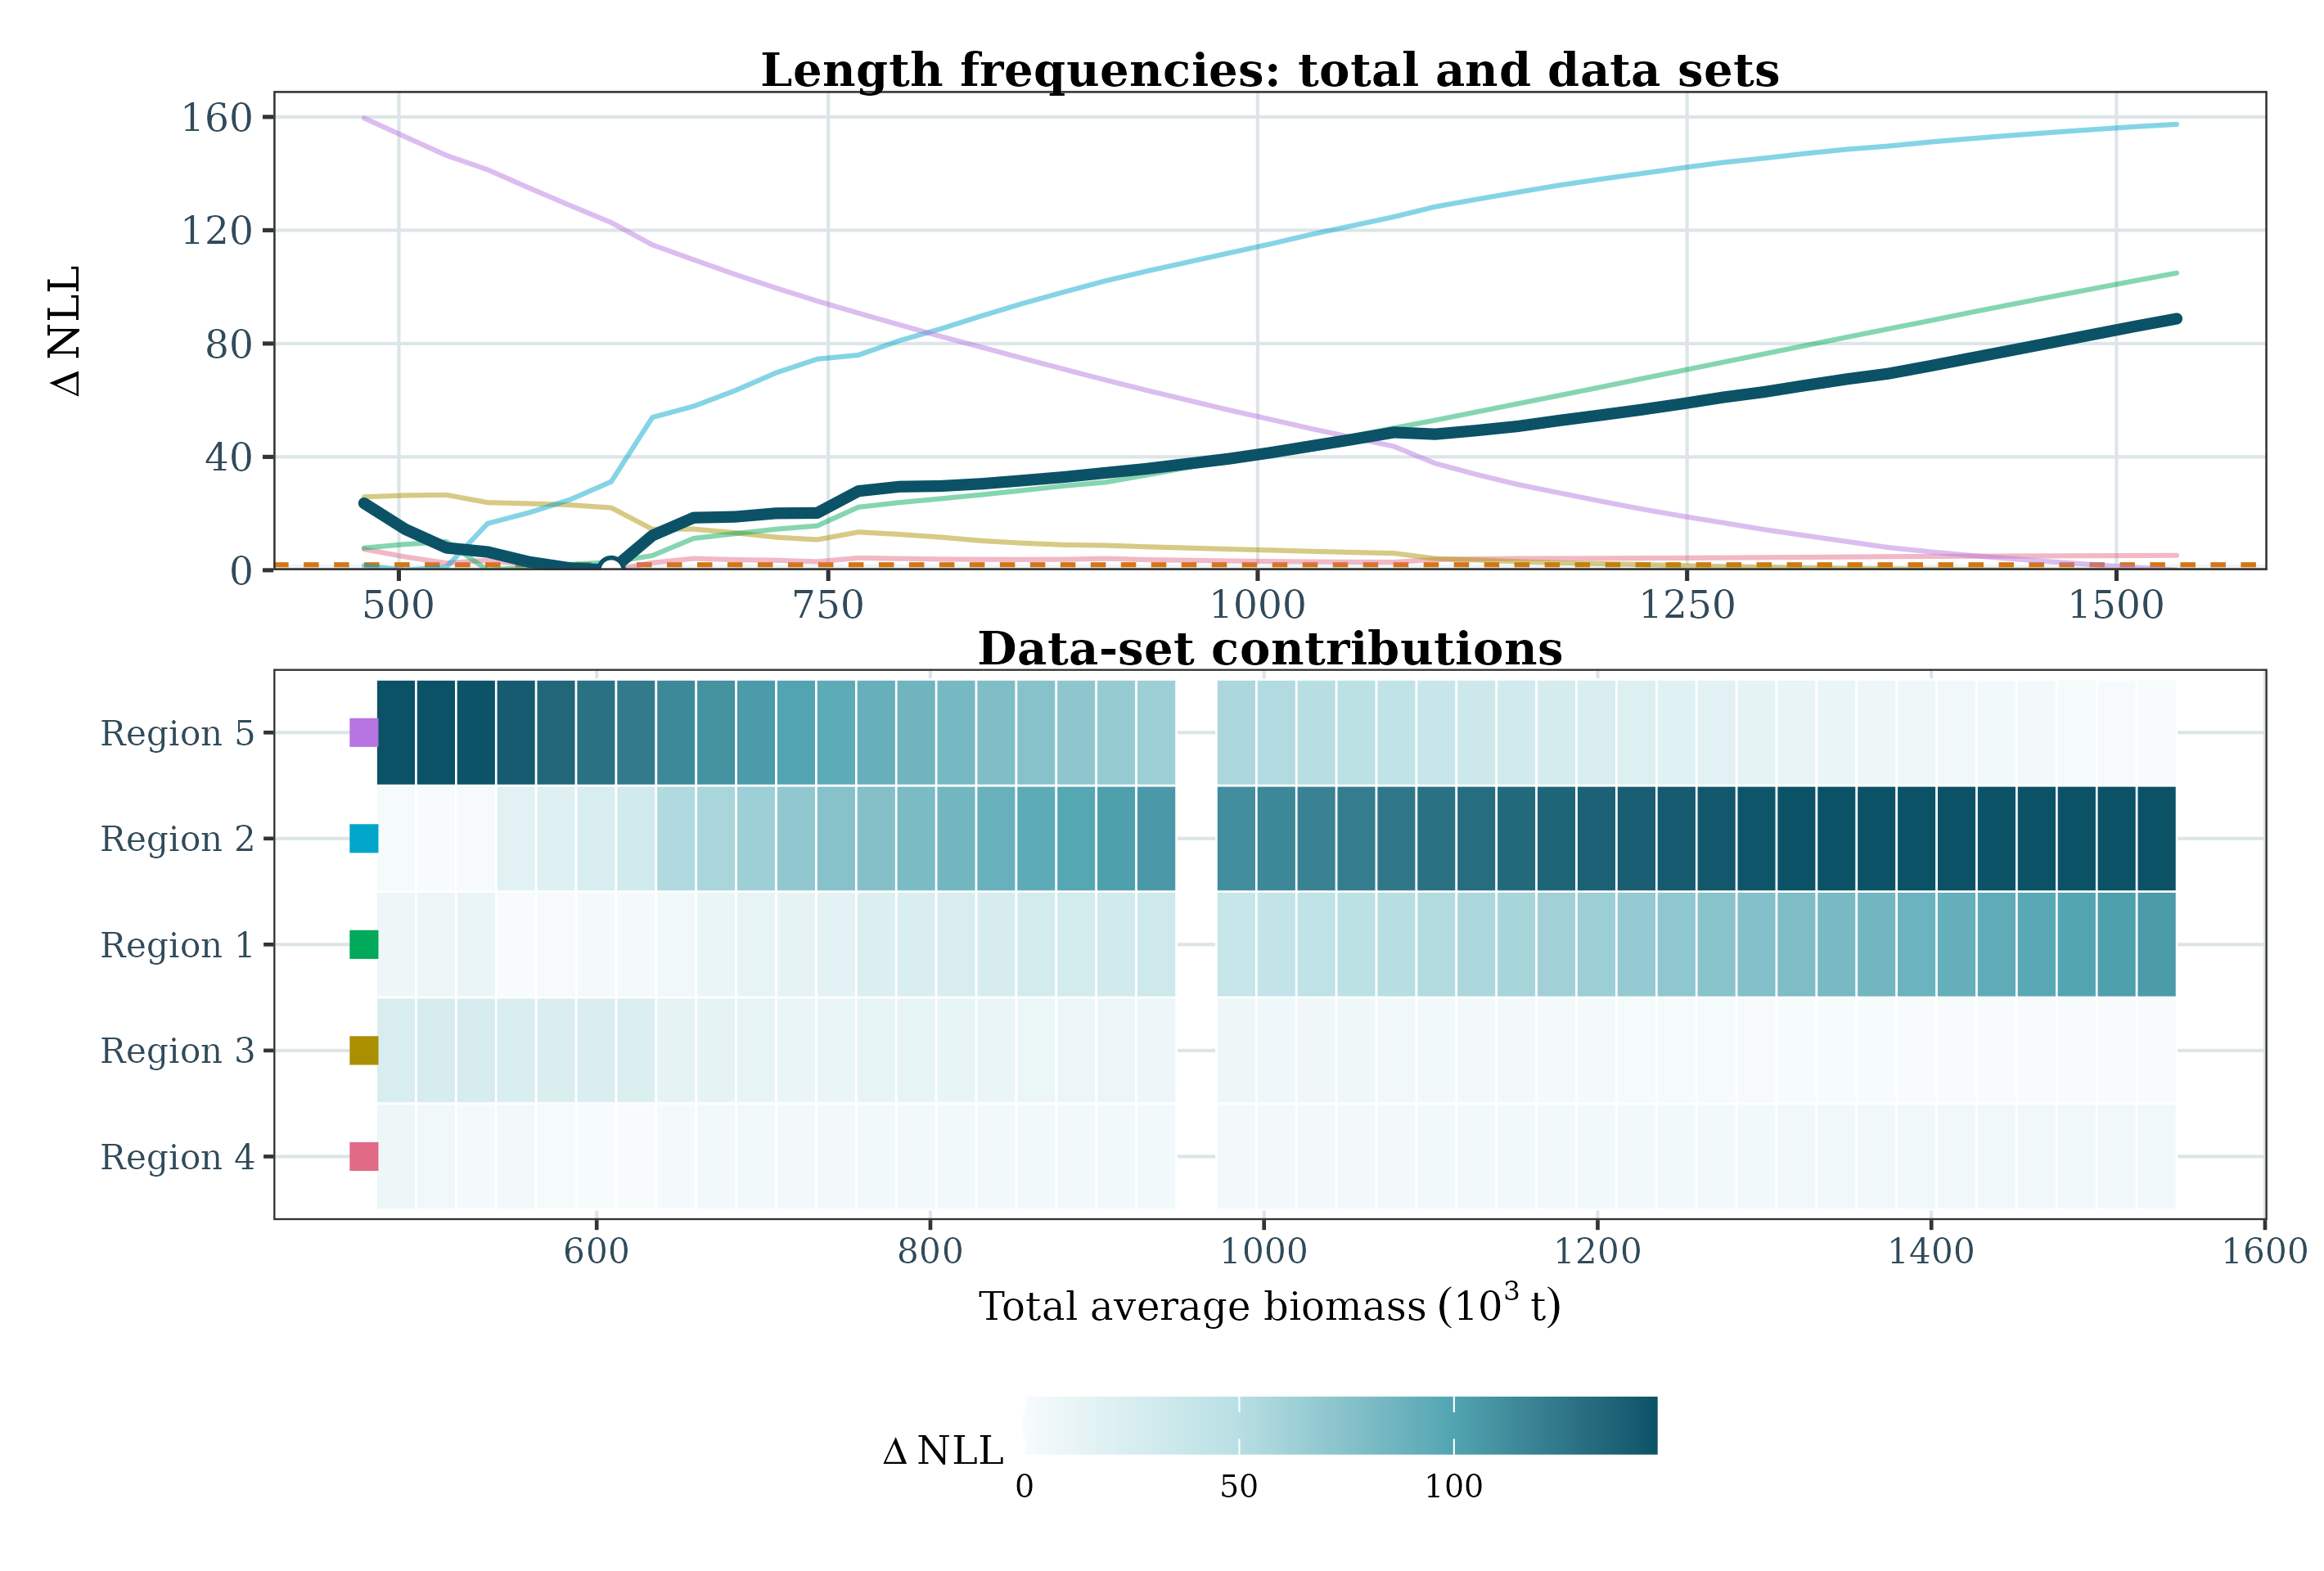
\includegraphics[width=1\linewidth,height=\textheight,keepaspectratio]{figures_new/likelihood-profile-lf-detail.png}

}

\caption{\label{fig-diag-profile-data-lf}Length-frequency likelihood
profile summarised by model region. The upper panel overlays the
prominent LF total with five thin regional curves; coloured row keys
connect them to the regional heatmap. Open a region in the
\href{https://pacificcommunity.github.io/ofp-sam-bet-2026-diagnostic/bet-2026-likelihood-profile-viewer.html}{interactive
profile viewer} for fishery-level curves.}

\end{figure}\DIFaddend %

\DIFdelbegin %DIFDELCMD < \begin{figure}[H]
%DIFDELCMD <

%DIFDELCMD < \centering{
%DIFDELCMD <

%DIFDELCMD < 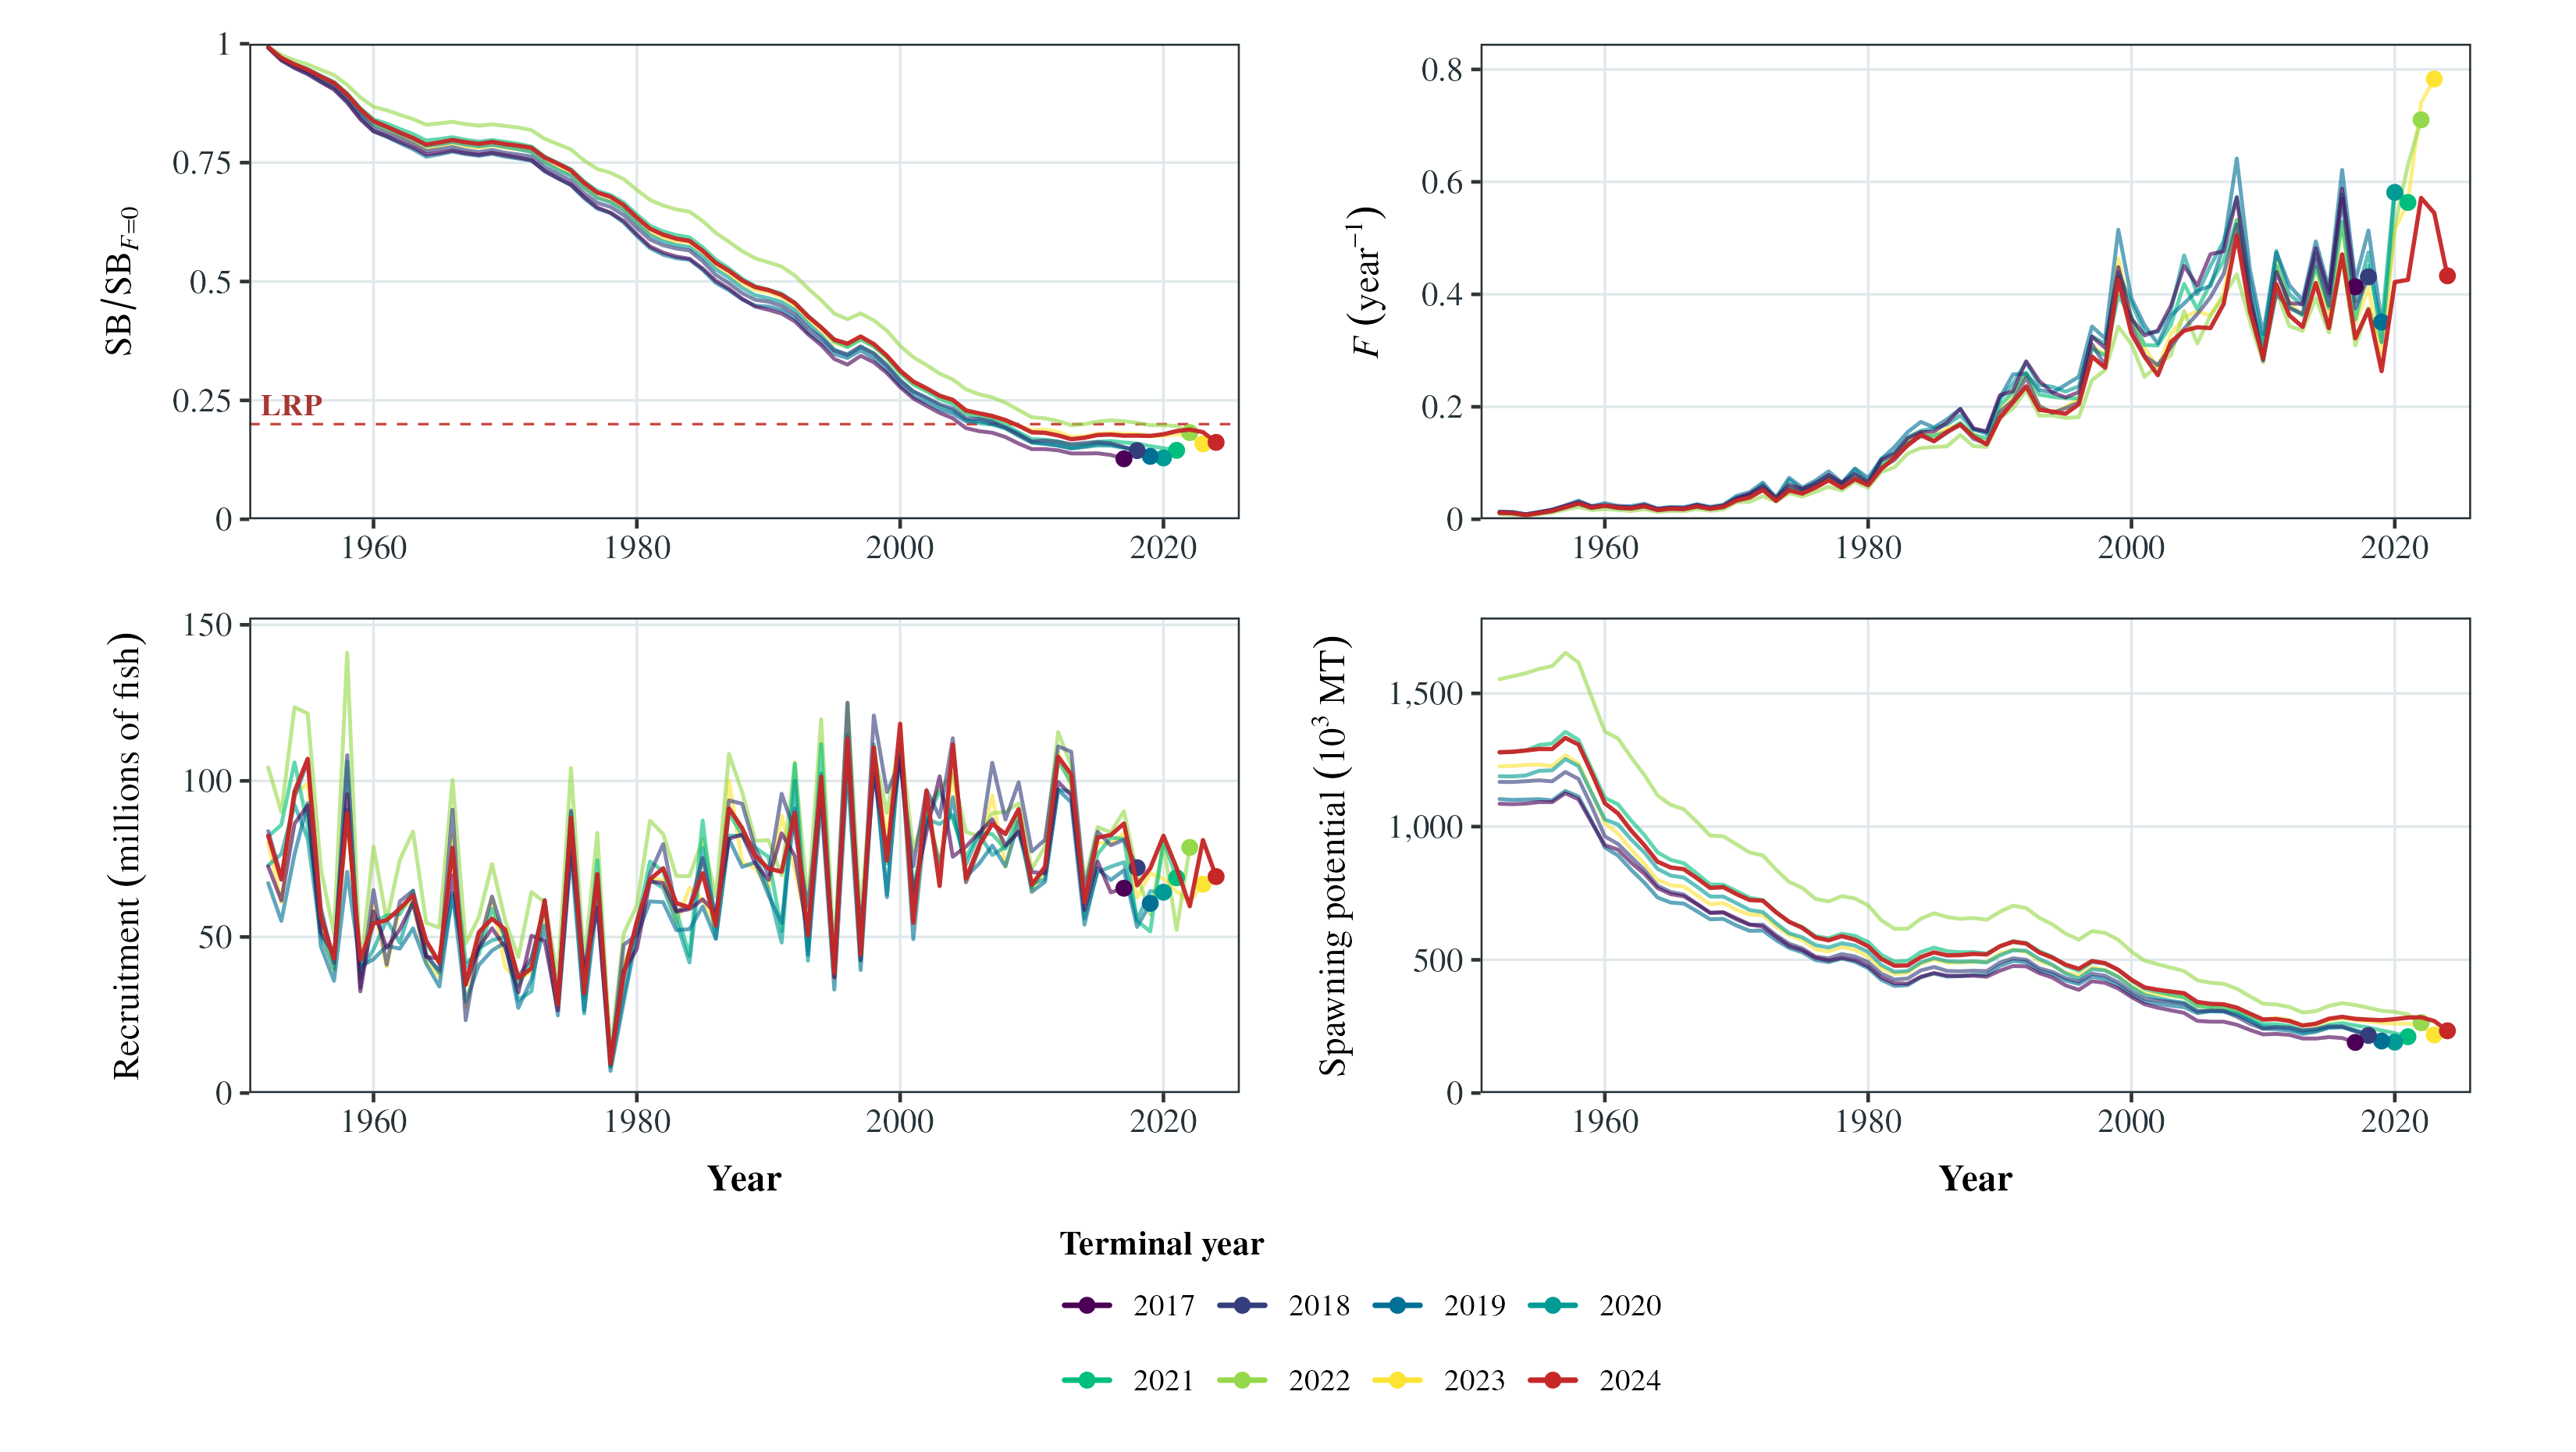
\includegraphics[width=1\linewidth,height=\textheight,keepaspectratio]{figures/retrospective_diag_panel.png}
%DIFDELCMD <

%DIFDELCMD < }
%DIFDELCMD <

%DIFDELCMD < \caption{\label{fig-retro-analysis}Retrospective estimates of depletion,
%DIFDELCMD < annual instantaneous fishing mortality, recruitment and spawning
%DIFDELCMD < potential for the Diagnostic model. The red line is the full-data fit;
%DIFDELCMD < the 7 converged retrospective peels are coloured by terminal year, with
%DIFDELCMD < points marking terminal estimates. The dashed line in the depletion
%DIFDELCMD < panel marks the limit reference point (\(SB\)/\(SB_{F=0}\) = 0.2).}
%DIFDELCMD <

%DIFDELCMD < \end{figure}%%%
\DIFdelend \DIFaddbegin \begin{figure}[H]

\centering{

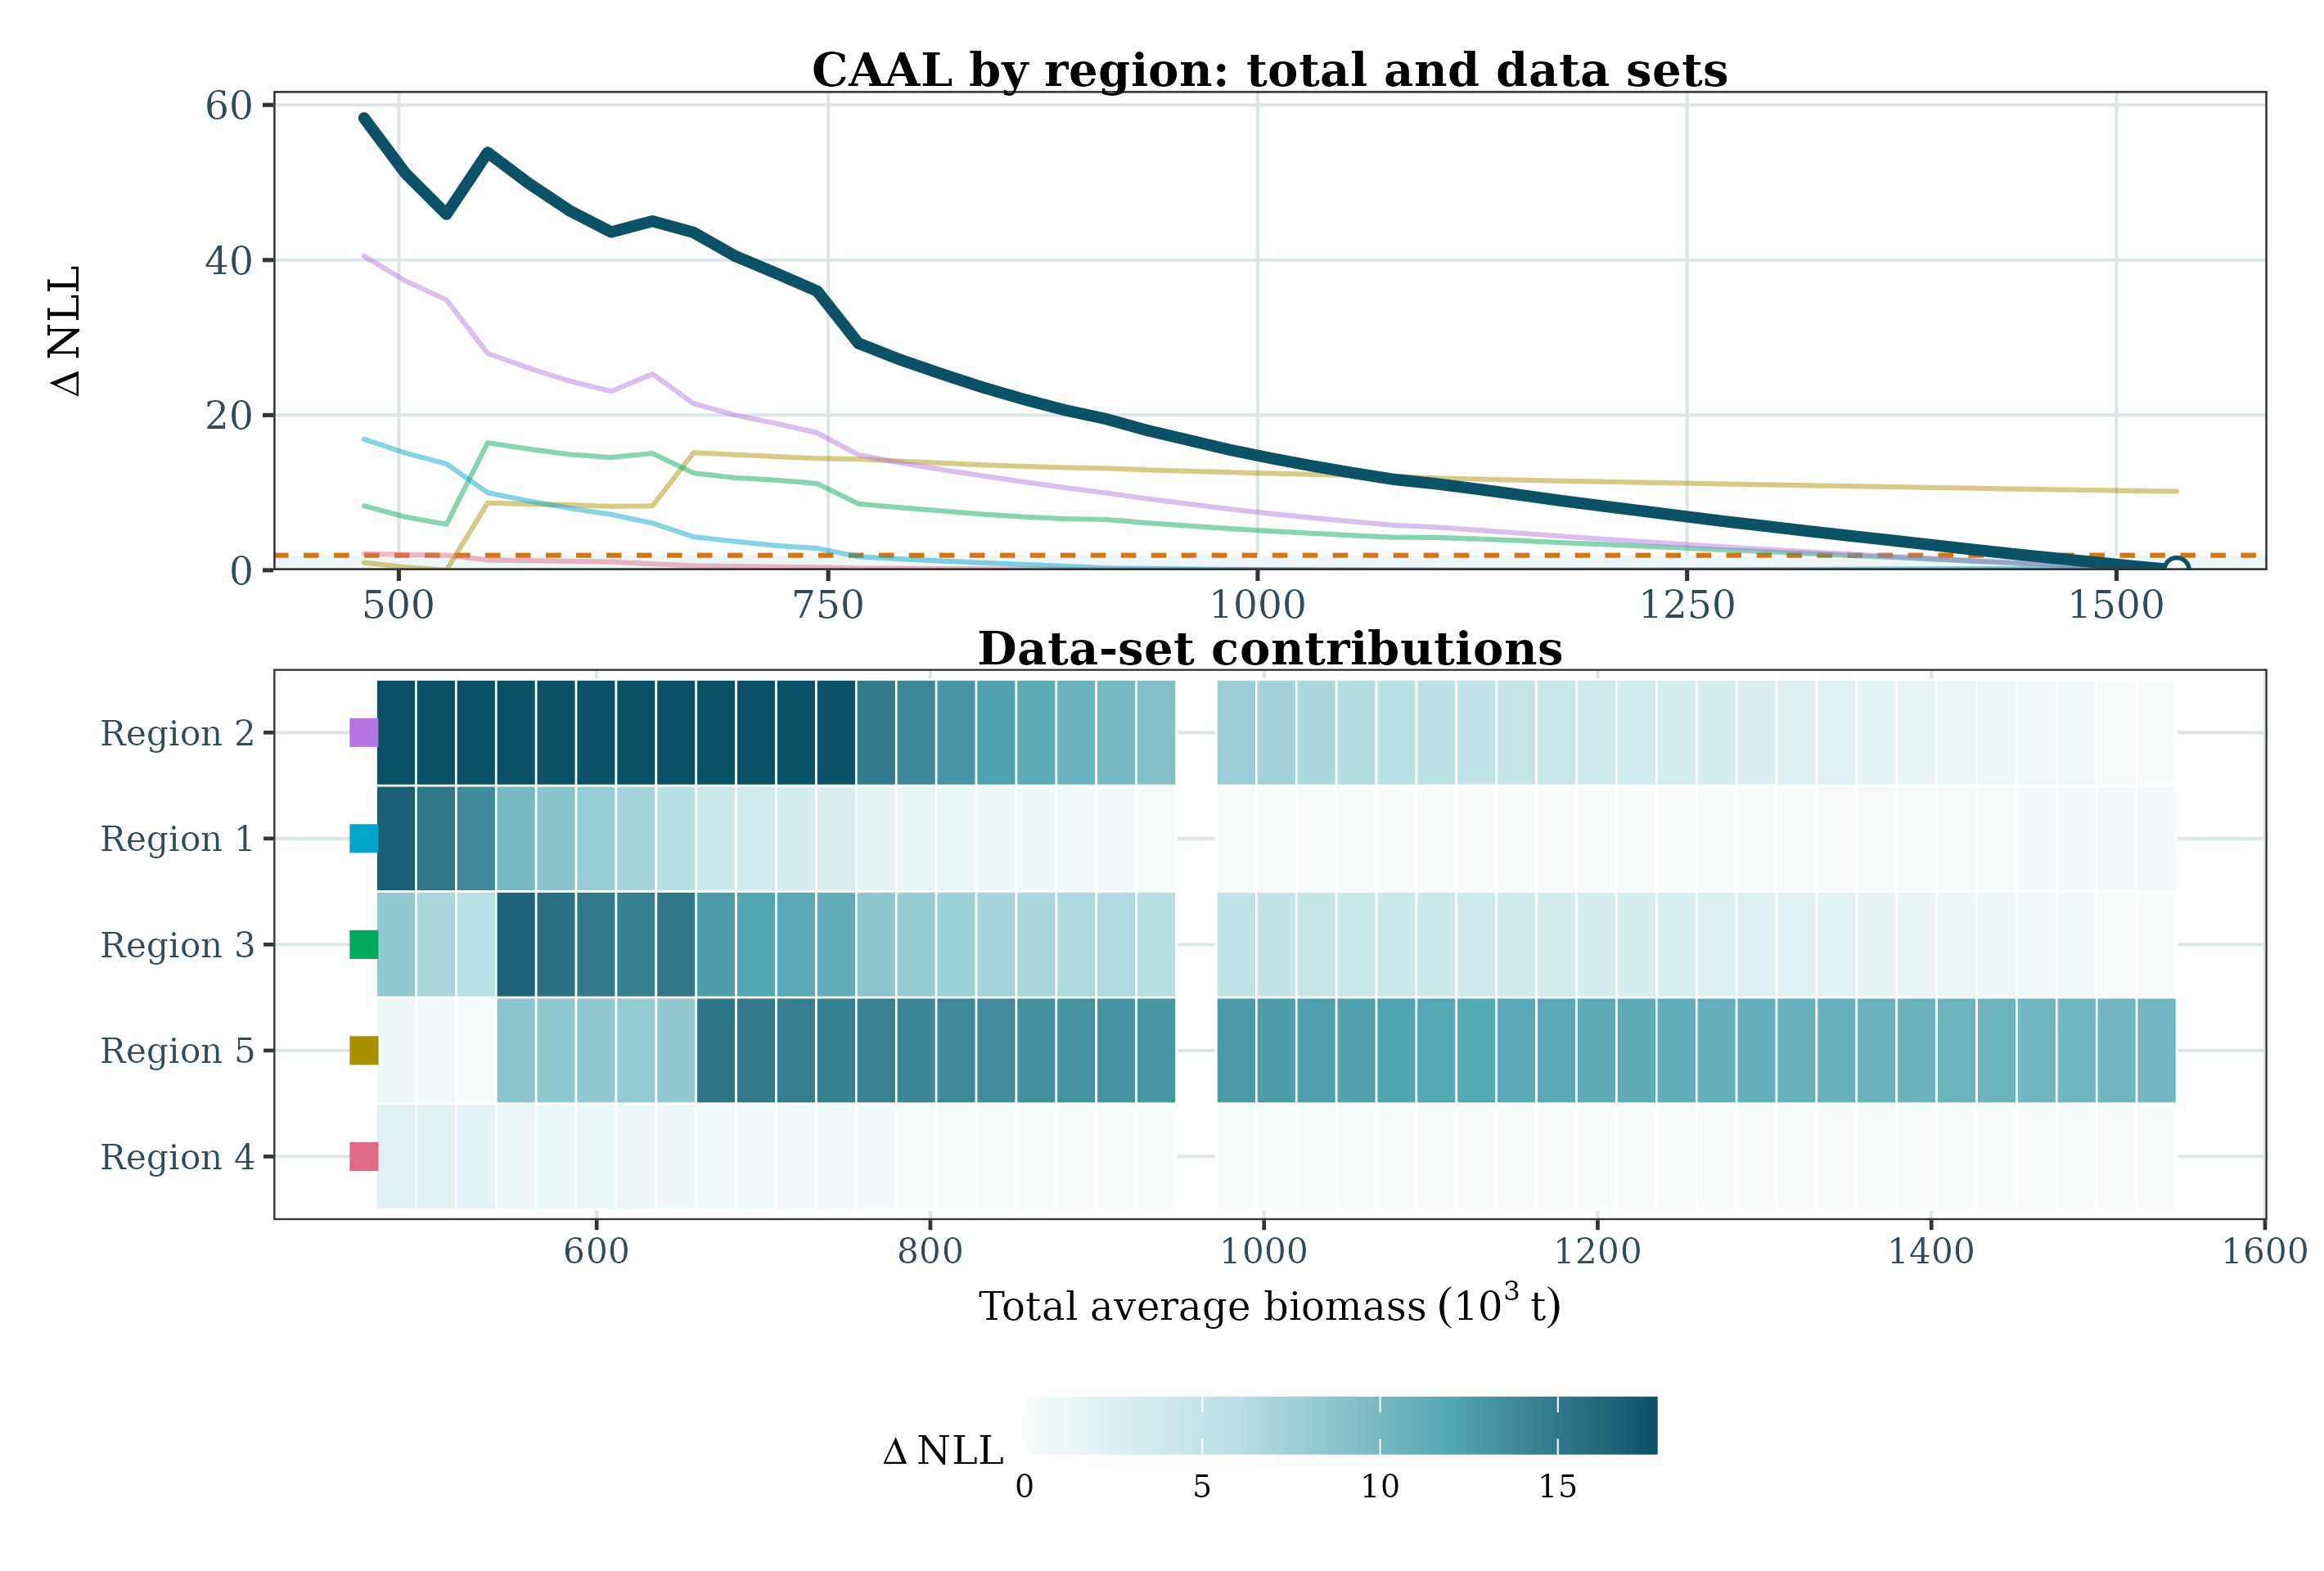
\includegraphics[width=1\linewidth,height=\textheight,keepaspectratio]{figures_new/likelihood-profile-caal-region-detail.png}

}

\caption{\label{fig-diag-profile-data-caal}Conditional age-at-length
likelihood profile. The upper panel overlays the prominent CAAL total
with thin regional curves; coloured row keys connect them to the five
heatmap contributions. Open a region in the
\href{https://pacificcommunity.github.io/ofp-sam-bet-2026-diagnostic/bet-2026-likelihood-profile-viewer.html}{interactive
profile viewer} for fishery-level curves.}

\end{figure}\DIFaddend %

\DIFdelbegin %DIFDELCMD < \begin{figure}[H]
%DIFDELCMD <

%DIFDELCMD < \centering{
%DIFDELCMD <

%DIFDELCMD < 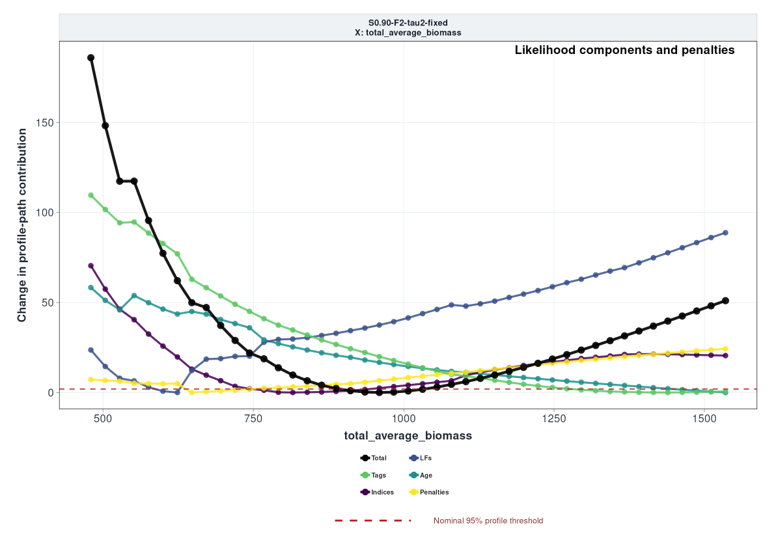
\includegraphics[width=1\linewidth,height=\textheight,keepaspectratio]{figures/diag_profile_data_sources.png}
%DIFDELCMD <

%DIFDELCMD < }
%DIFDELCMD <

%DIFDELCMD < \caption{\label{fig-diag-profile-data-sources}Diagnostic model
%DIFDELCMD < likelihood profile of average total biomass in million mt. The black
%DIFDELCMD < line indicates the total likelihood with the colours representing
%DIFDELCMD < component of the total likelihood coming from different data sources.}
%DIFDELCMD <

%DIFDELCMD < \end{figure}%%%
\DIFdelend \DIFaddbegin \begin{figure}[H]

\centering{

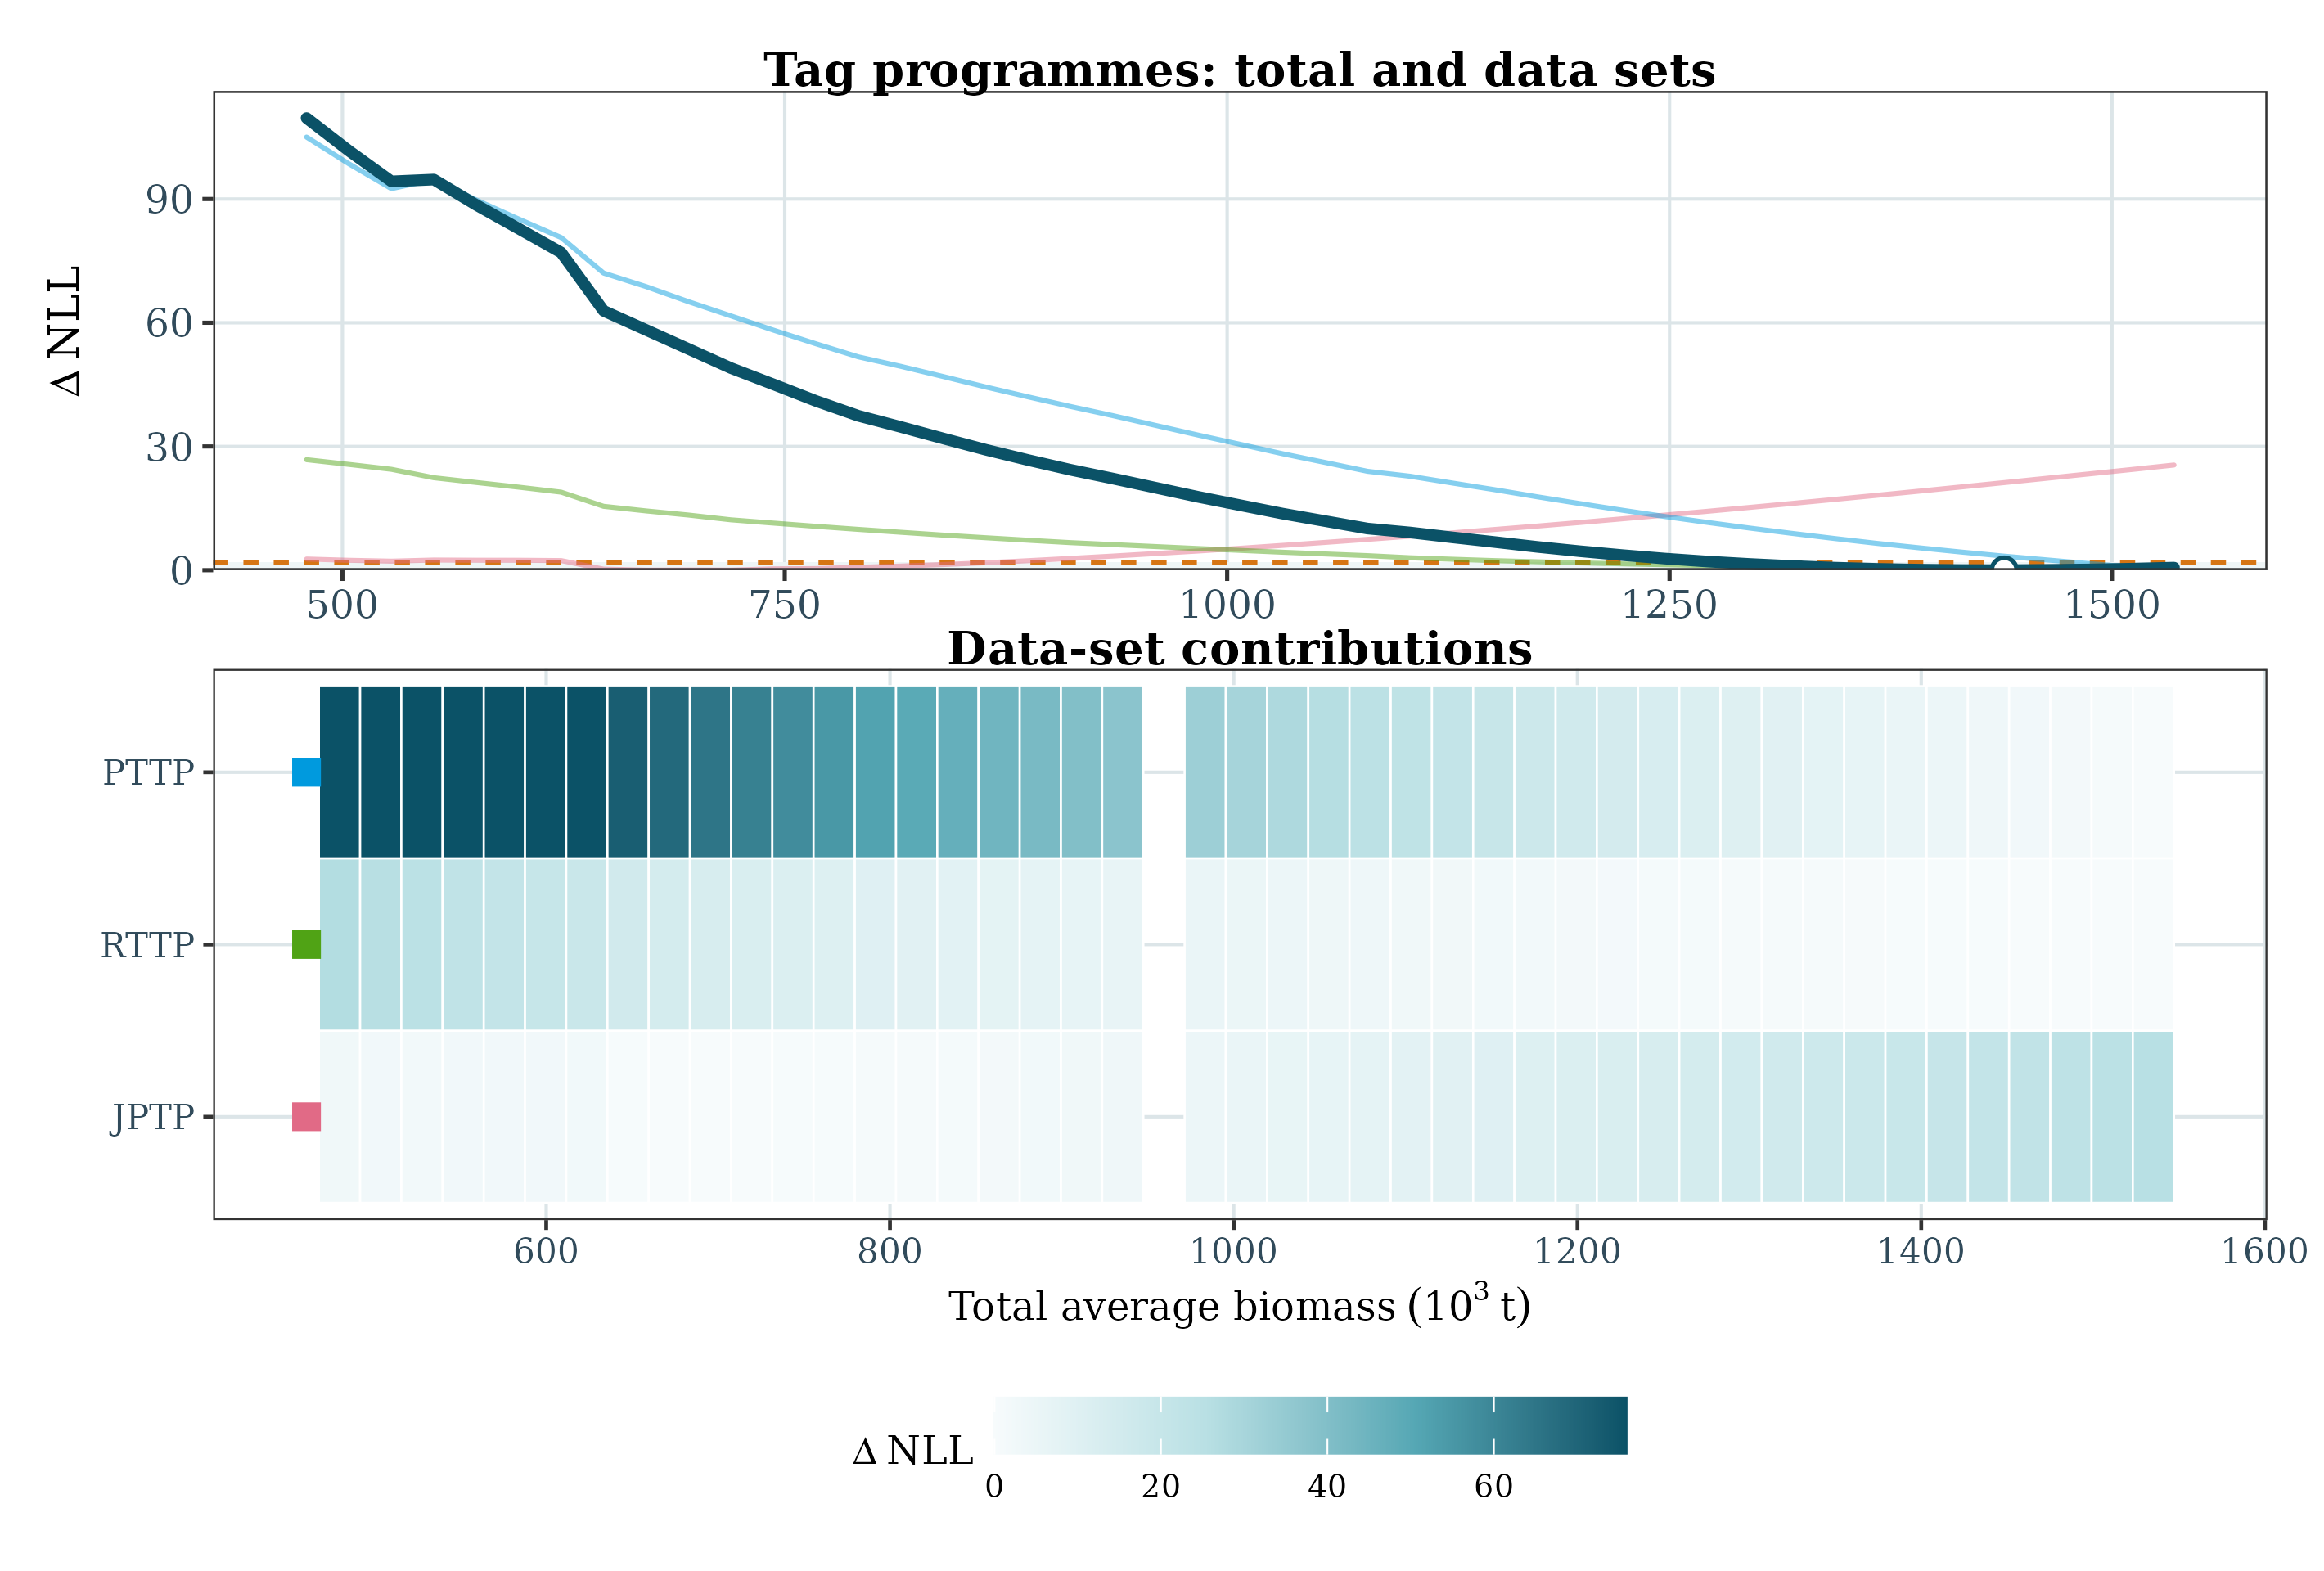
\includegraphics[width=1\linewidth,height=\textheight,keepaspectratio]{figures_new/likelihood-profile-tag-detail.png}

}

\caption{\label{fig-diag-profile-data-tag-prog}\label{fig-diag-profile-data-tag-prog-grps}Tag likelihood profile.
The upper panel overlays the prominent tag total with thin programme
curves; coloured row keys connect them to the RTTP, PTTP and JPTP
heatmap contributions. Open a programme in the
\href{https://pacificcommunity.github.io/ofp-sam-bet-2026-diagnostic/bet-2026-likelihood-profile-viewer.html}{interactive
profile viewer} for release-group curves.}

\end{figure}\DIFaddend %

\DIFdelbegin %DIFDELCMD < \begin{figure}[H]
%DIFDELCMD <

%DIFDELCMD < \centering{
%DIFDELCMD <

%DIFDELCMD < 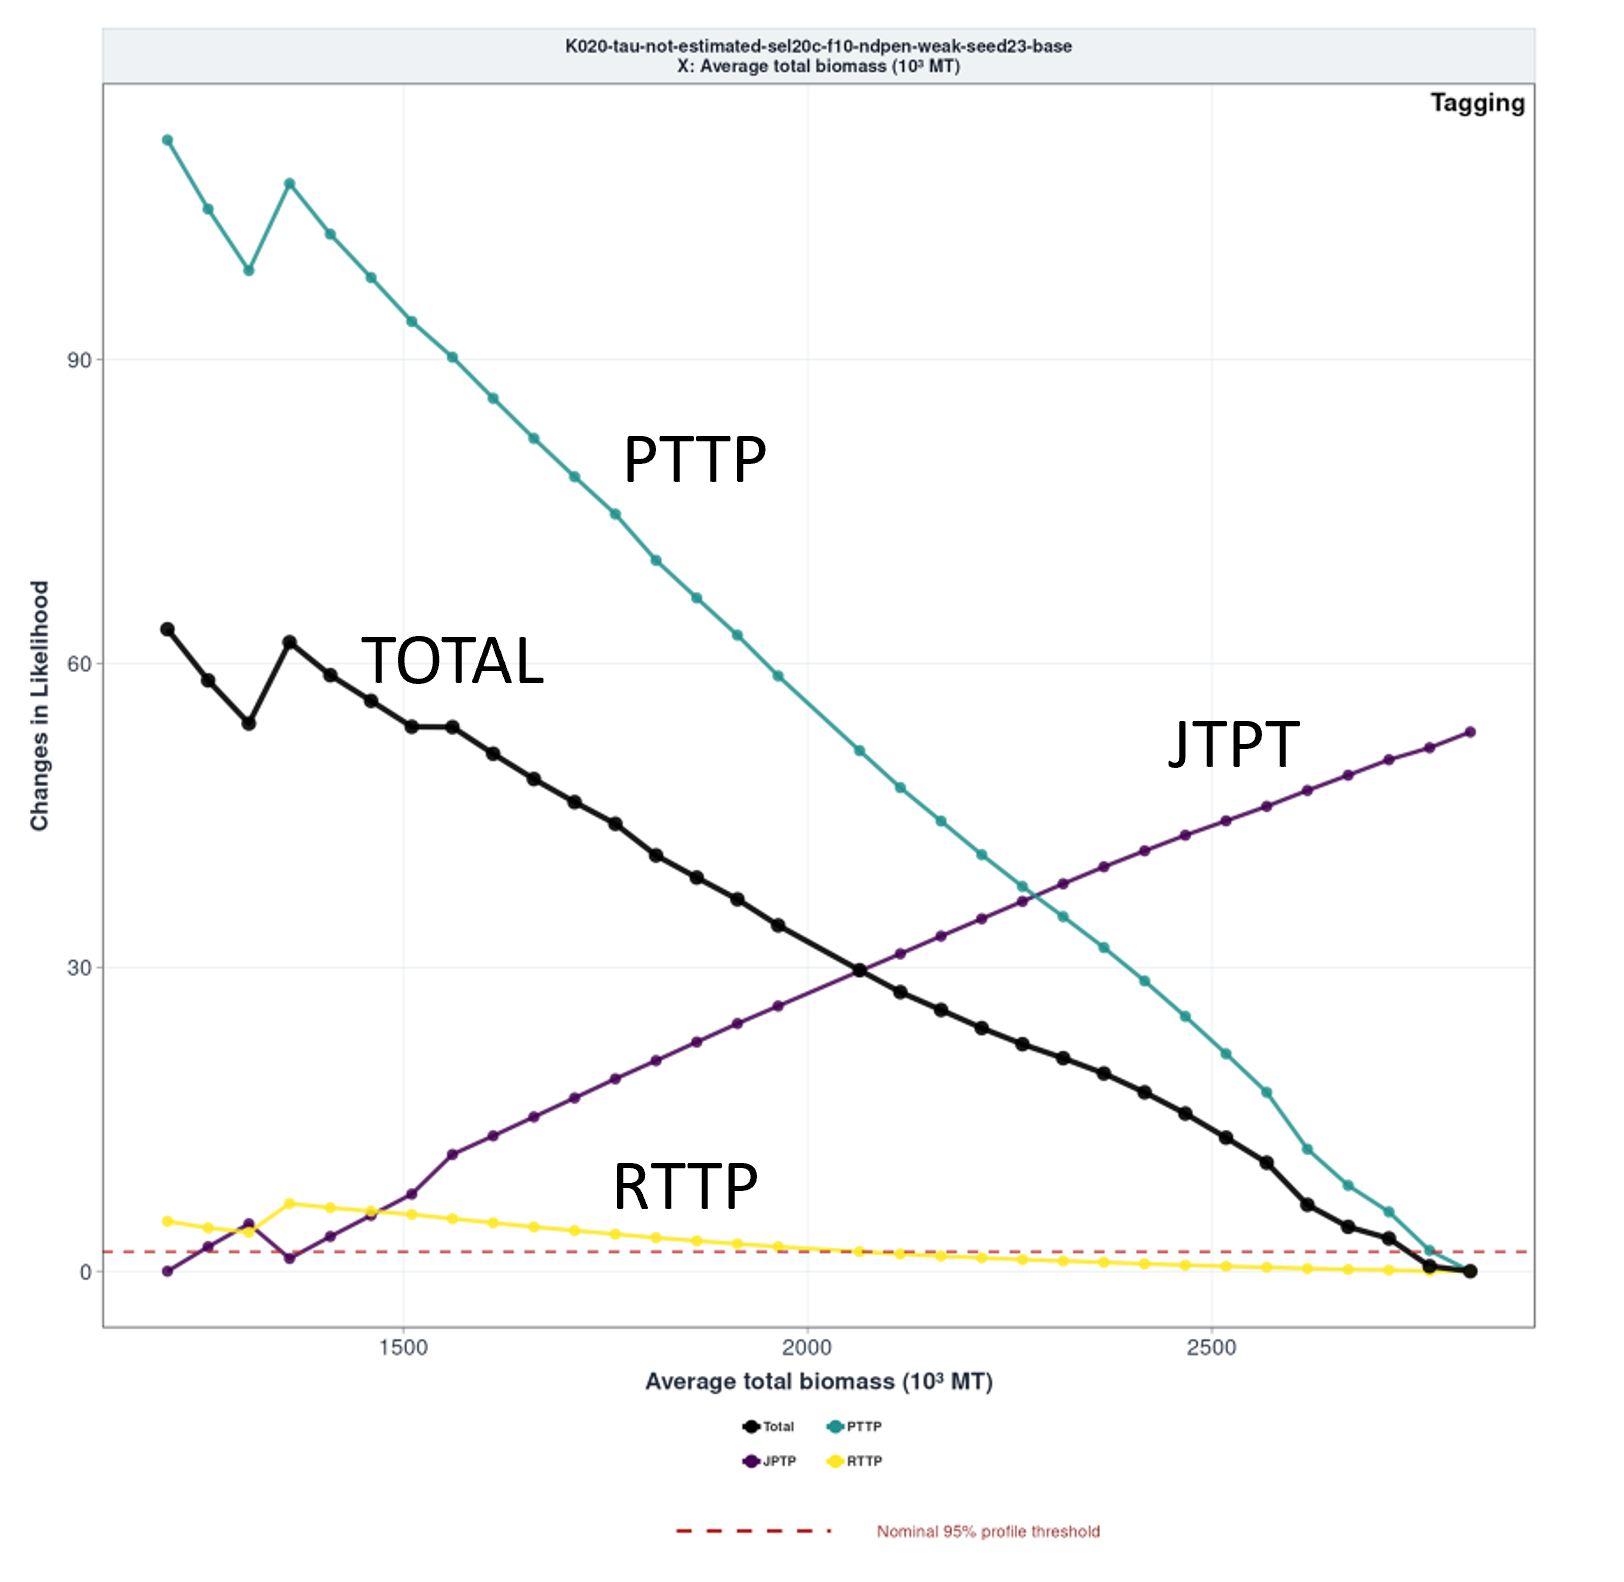
\includegraphics[width=1\linewidth,height=\textheight,keepaspectratio]{figures/diag_profile_data_tag_programmes.png}
%DIFDELCMD <

%DIFDELCMD < }
%DIFDELCMD <

%DIFDELCMD < \caption{\label{fig-diag-profile-data-tag-prog}\label{fig-diag-profile-data-tag-prog-grps}Diagnostic model
%DIFDELCMD < likelihood profile of average total biomass in million mt. The black
%DIFDELCMD < line indicates the total likelihood with the colours representing
%DIFDELCMD < component of the total likelihood coming from different tag programmes.}
%DIFDELCMD <

%DIFDELCMD < \end{figure}%%%
\DIFdelend \DIFaddbegin \begin{figure}[H]

\centering{

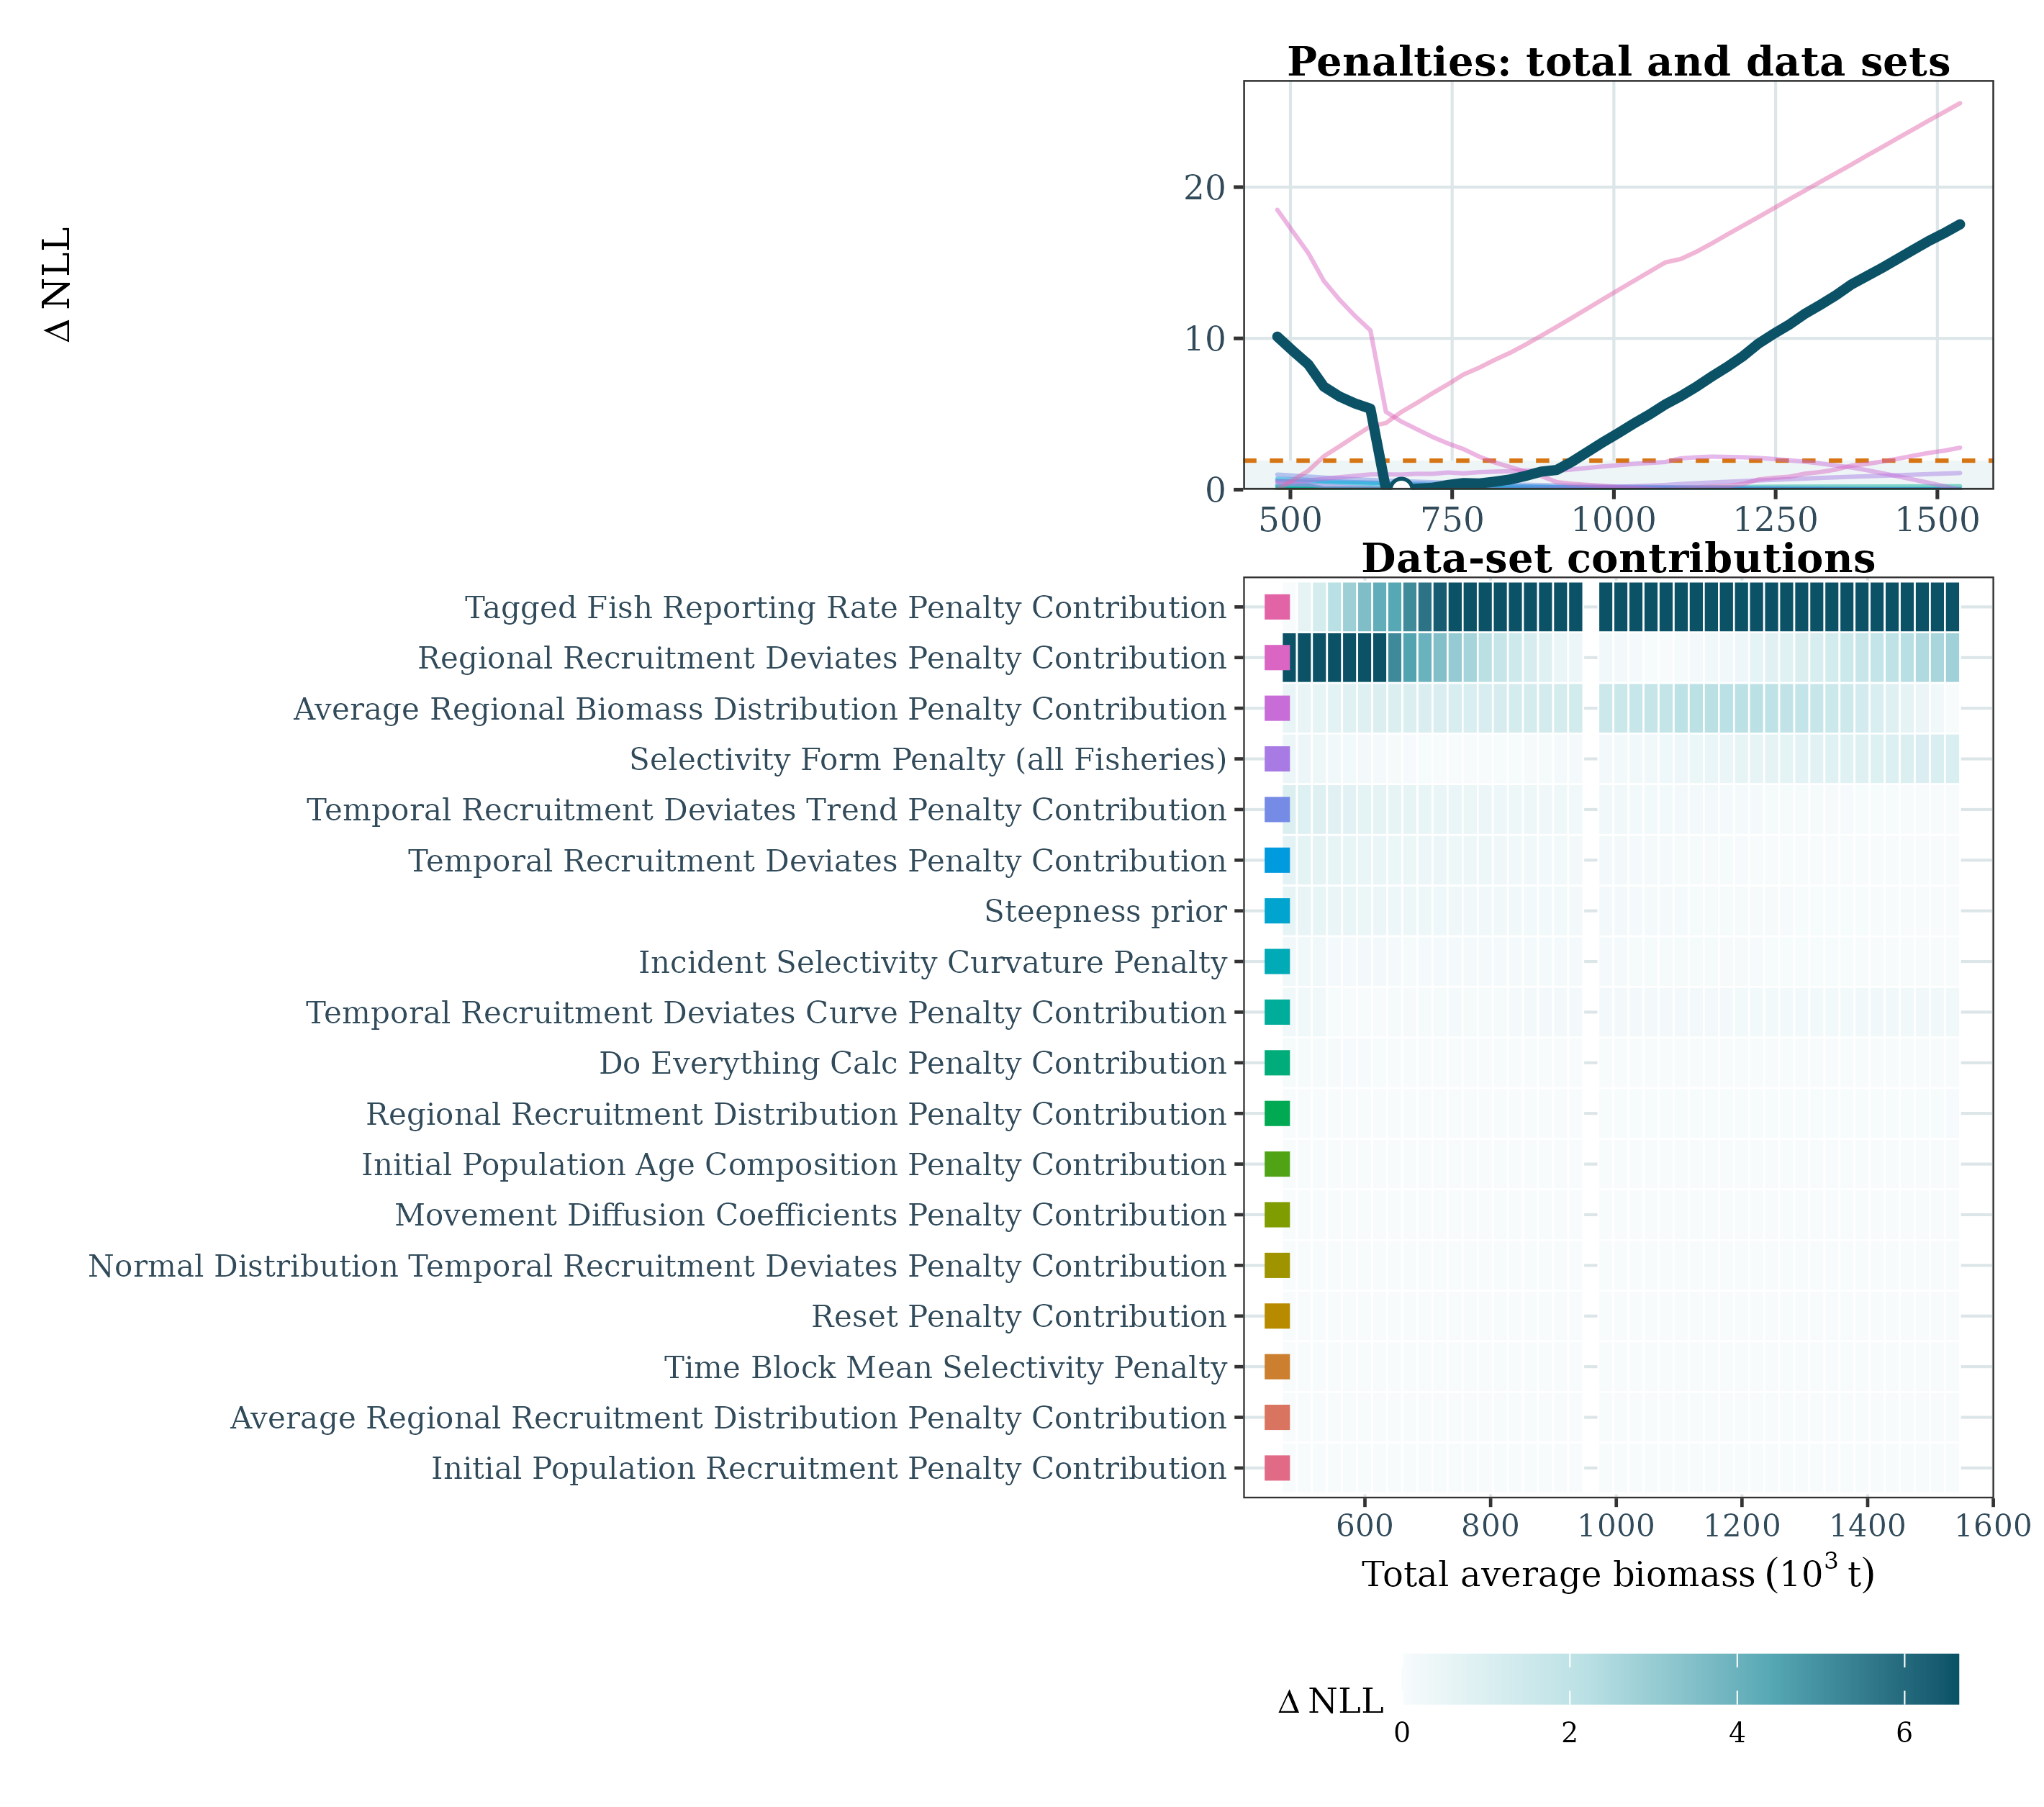
\includegraphics[width=1\linewidth,height=\textheight,keepaspectratio]{figures_new/likelihood-profile-penalty-detail.png}

}

\caption{\label{fig-diag-profile-data-penalty}Penalty likelihood
profile. The upper panel overlays the prominent penalty total with thin,
translucent component curves; coloured row keys connect them to the
heatmap while limiting visual clutter. Open the
\href{https://pacificcommunity.github.io/ofp-sam-bet-2026-diagnostic/bet-2026-likelihood-profile-viewer.html}{interactive
profile viewer} to select a component.}

\end{figure}\DIFaddend %

\DIFdelbegin %DIFDELCMD < \begin{figure}[H]
%DIFDELCMD <

%DIFDELCMD < \centering{
%DIFDELCMD <

%DIFDELCMD < 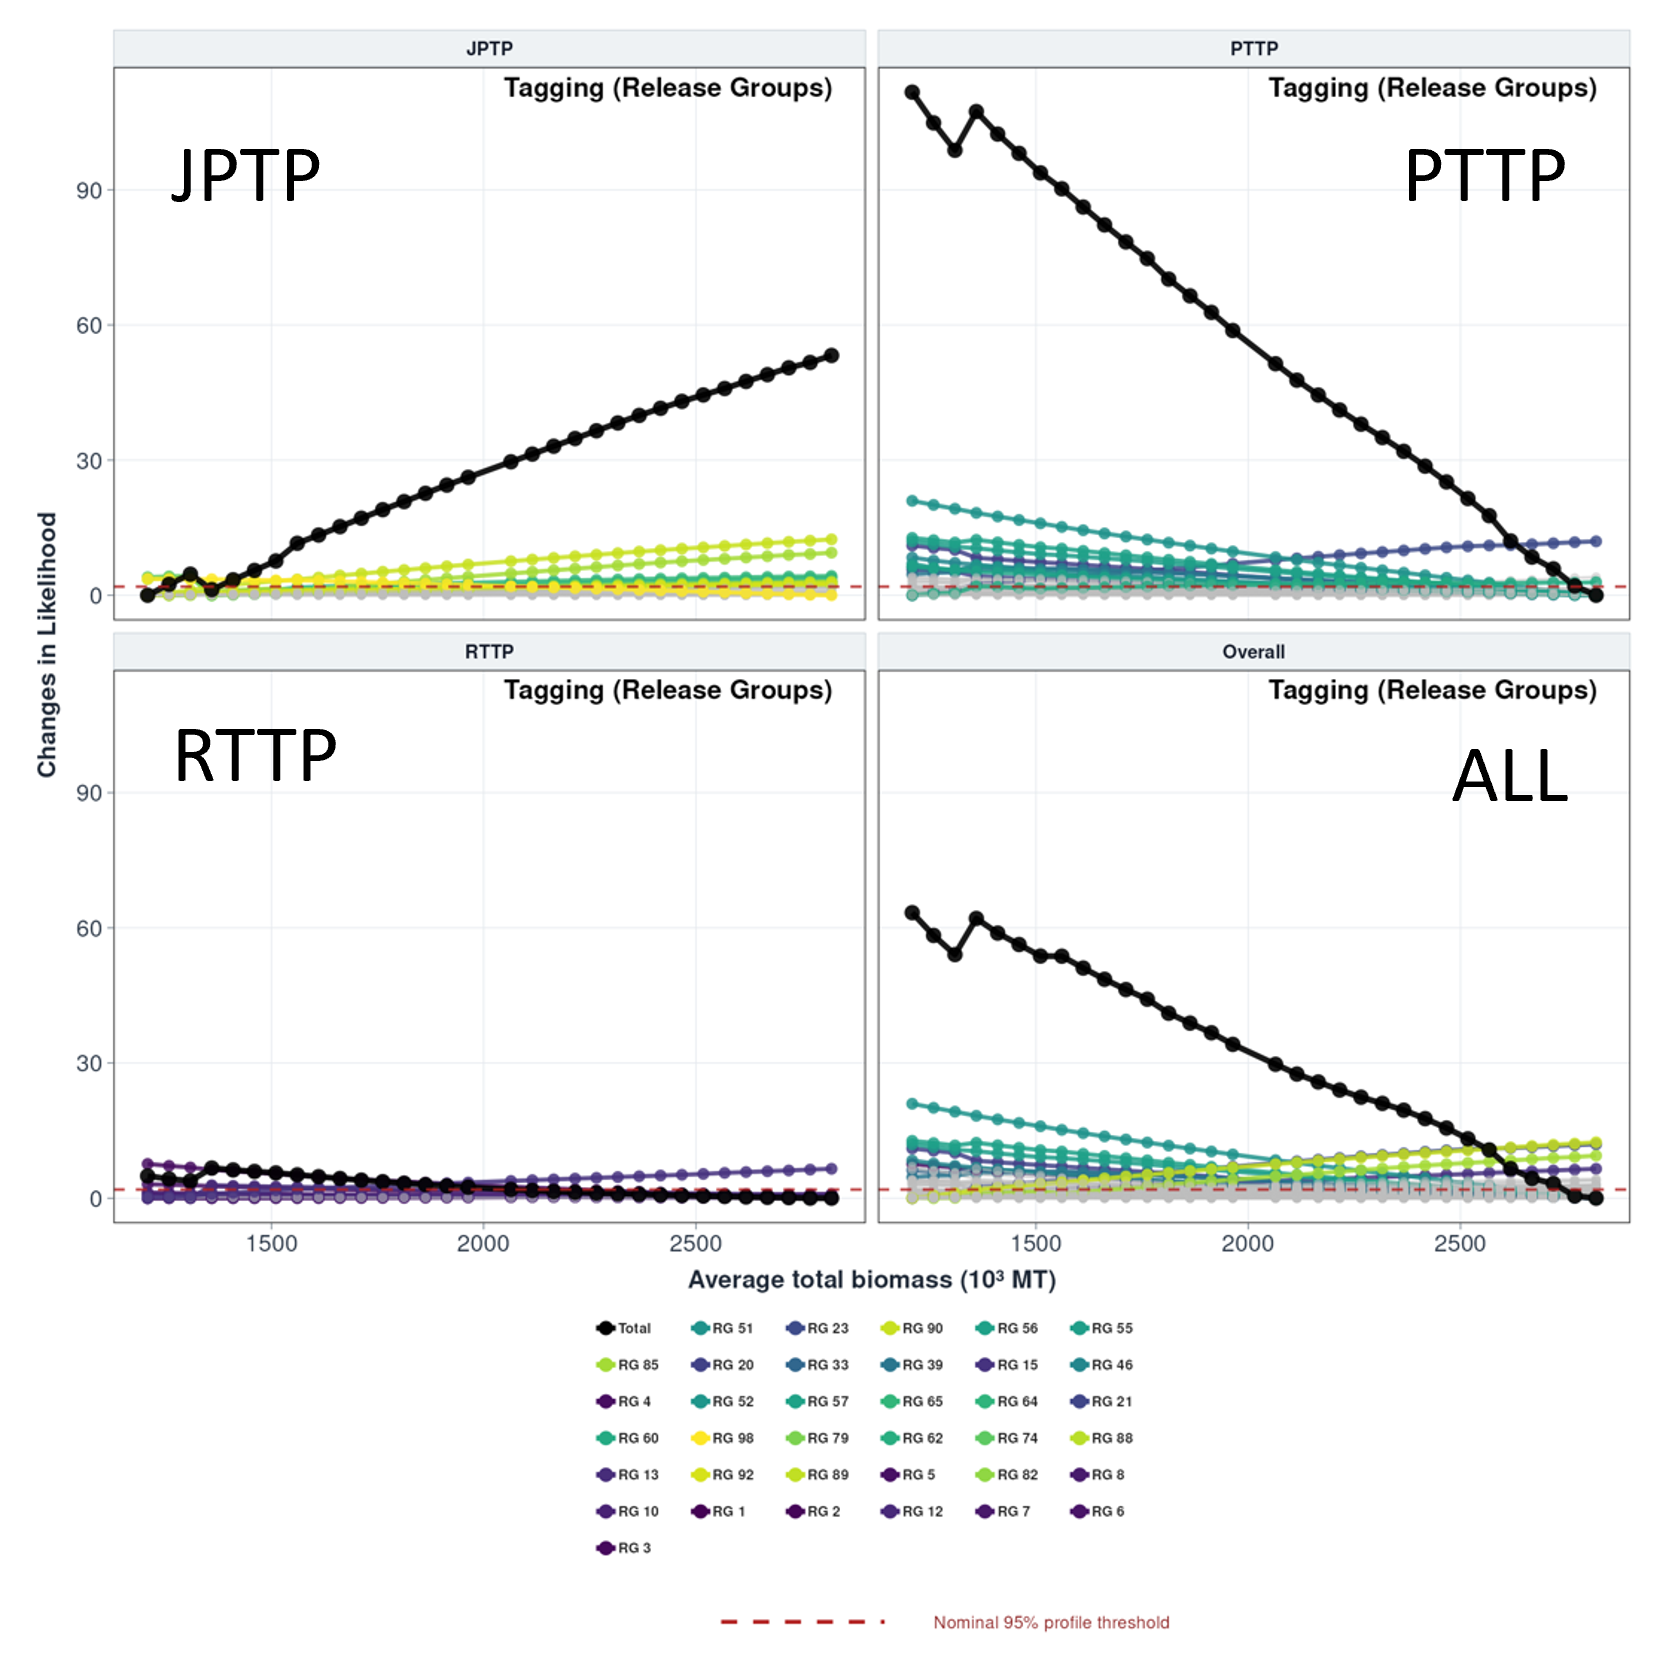
\includegraphics[width=1\linewidth,height=\textheight,keepaspectratio]{figures/diag_profile_data_tag_rel_groups.png}
%DIFDELCMD <

%DIFDELCMD < }
%DIFDELCMD <

%DIFDELCMD < \caption{\label{fig-diag-profile-data-tag-prog-grps}Diagnostic model
%DIFDELCMD < likelihood profile of average total biomass in million mt. The black
%DIFDELCMD < line indicates the total likelihood with the colours representing
%DIFDELCMD < component of the total likelihood coming from different tag release
%DIFDELCMD < groups.}
%DIFDELCMD <

%DIFDELCMD < \end{figure}%%%
\DIFdelend \DIFaddbegin \begin{figure}[H]

\centering{

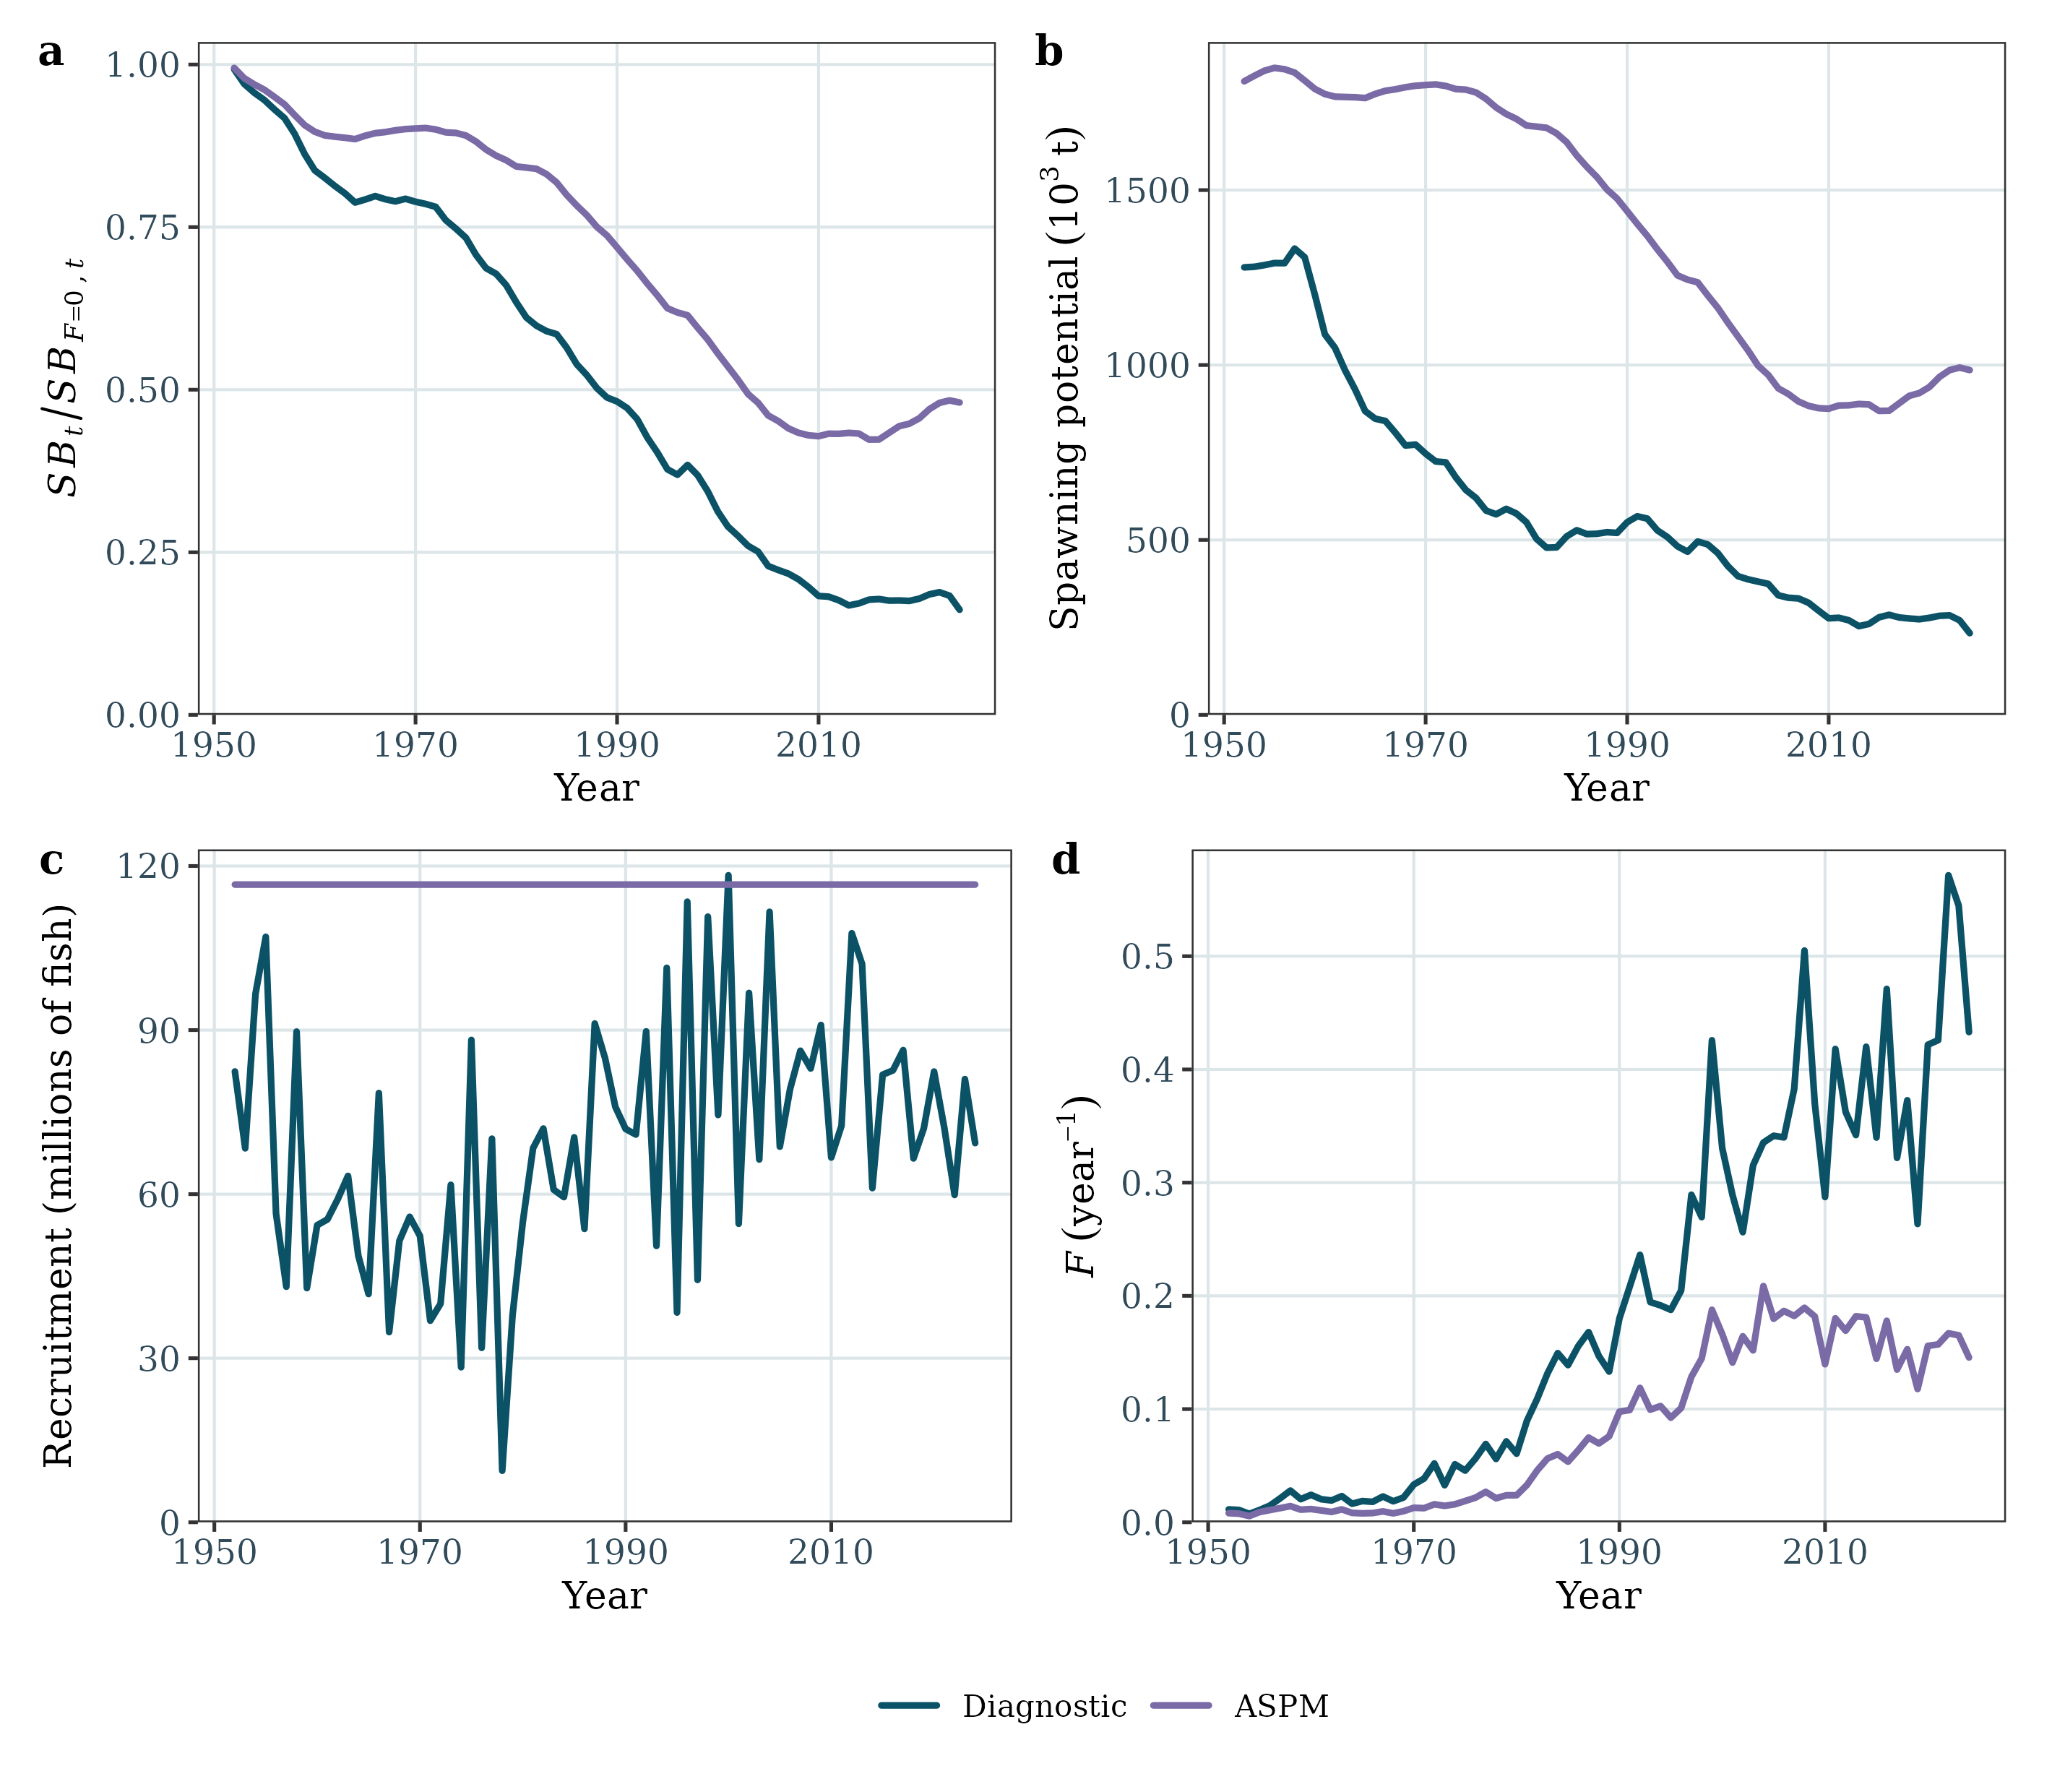
\includegraphics[width=1\linewidth,height=\textheight,keepaspectratio]{figures_new/aspm-comparison.png}

}

\caption{\label{fig-aspm-comparison}Comparison of the diagnostic model
and constant-recruitment age-structured production model (ASPM): (a)
dynamic spawning depletion, (b) spawning potential, (c) recruitment and
(d) annual population-weighted fishing mortality.}

\end{figure}\DIFaddend %

\DIFdelbegin %DIFDELCMD < \begin{figure}[H]
%DIFDELCMD <

%DIFDELCMD < \centering{
%DIFDELCMD <

%DIFDELCMD < 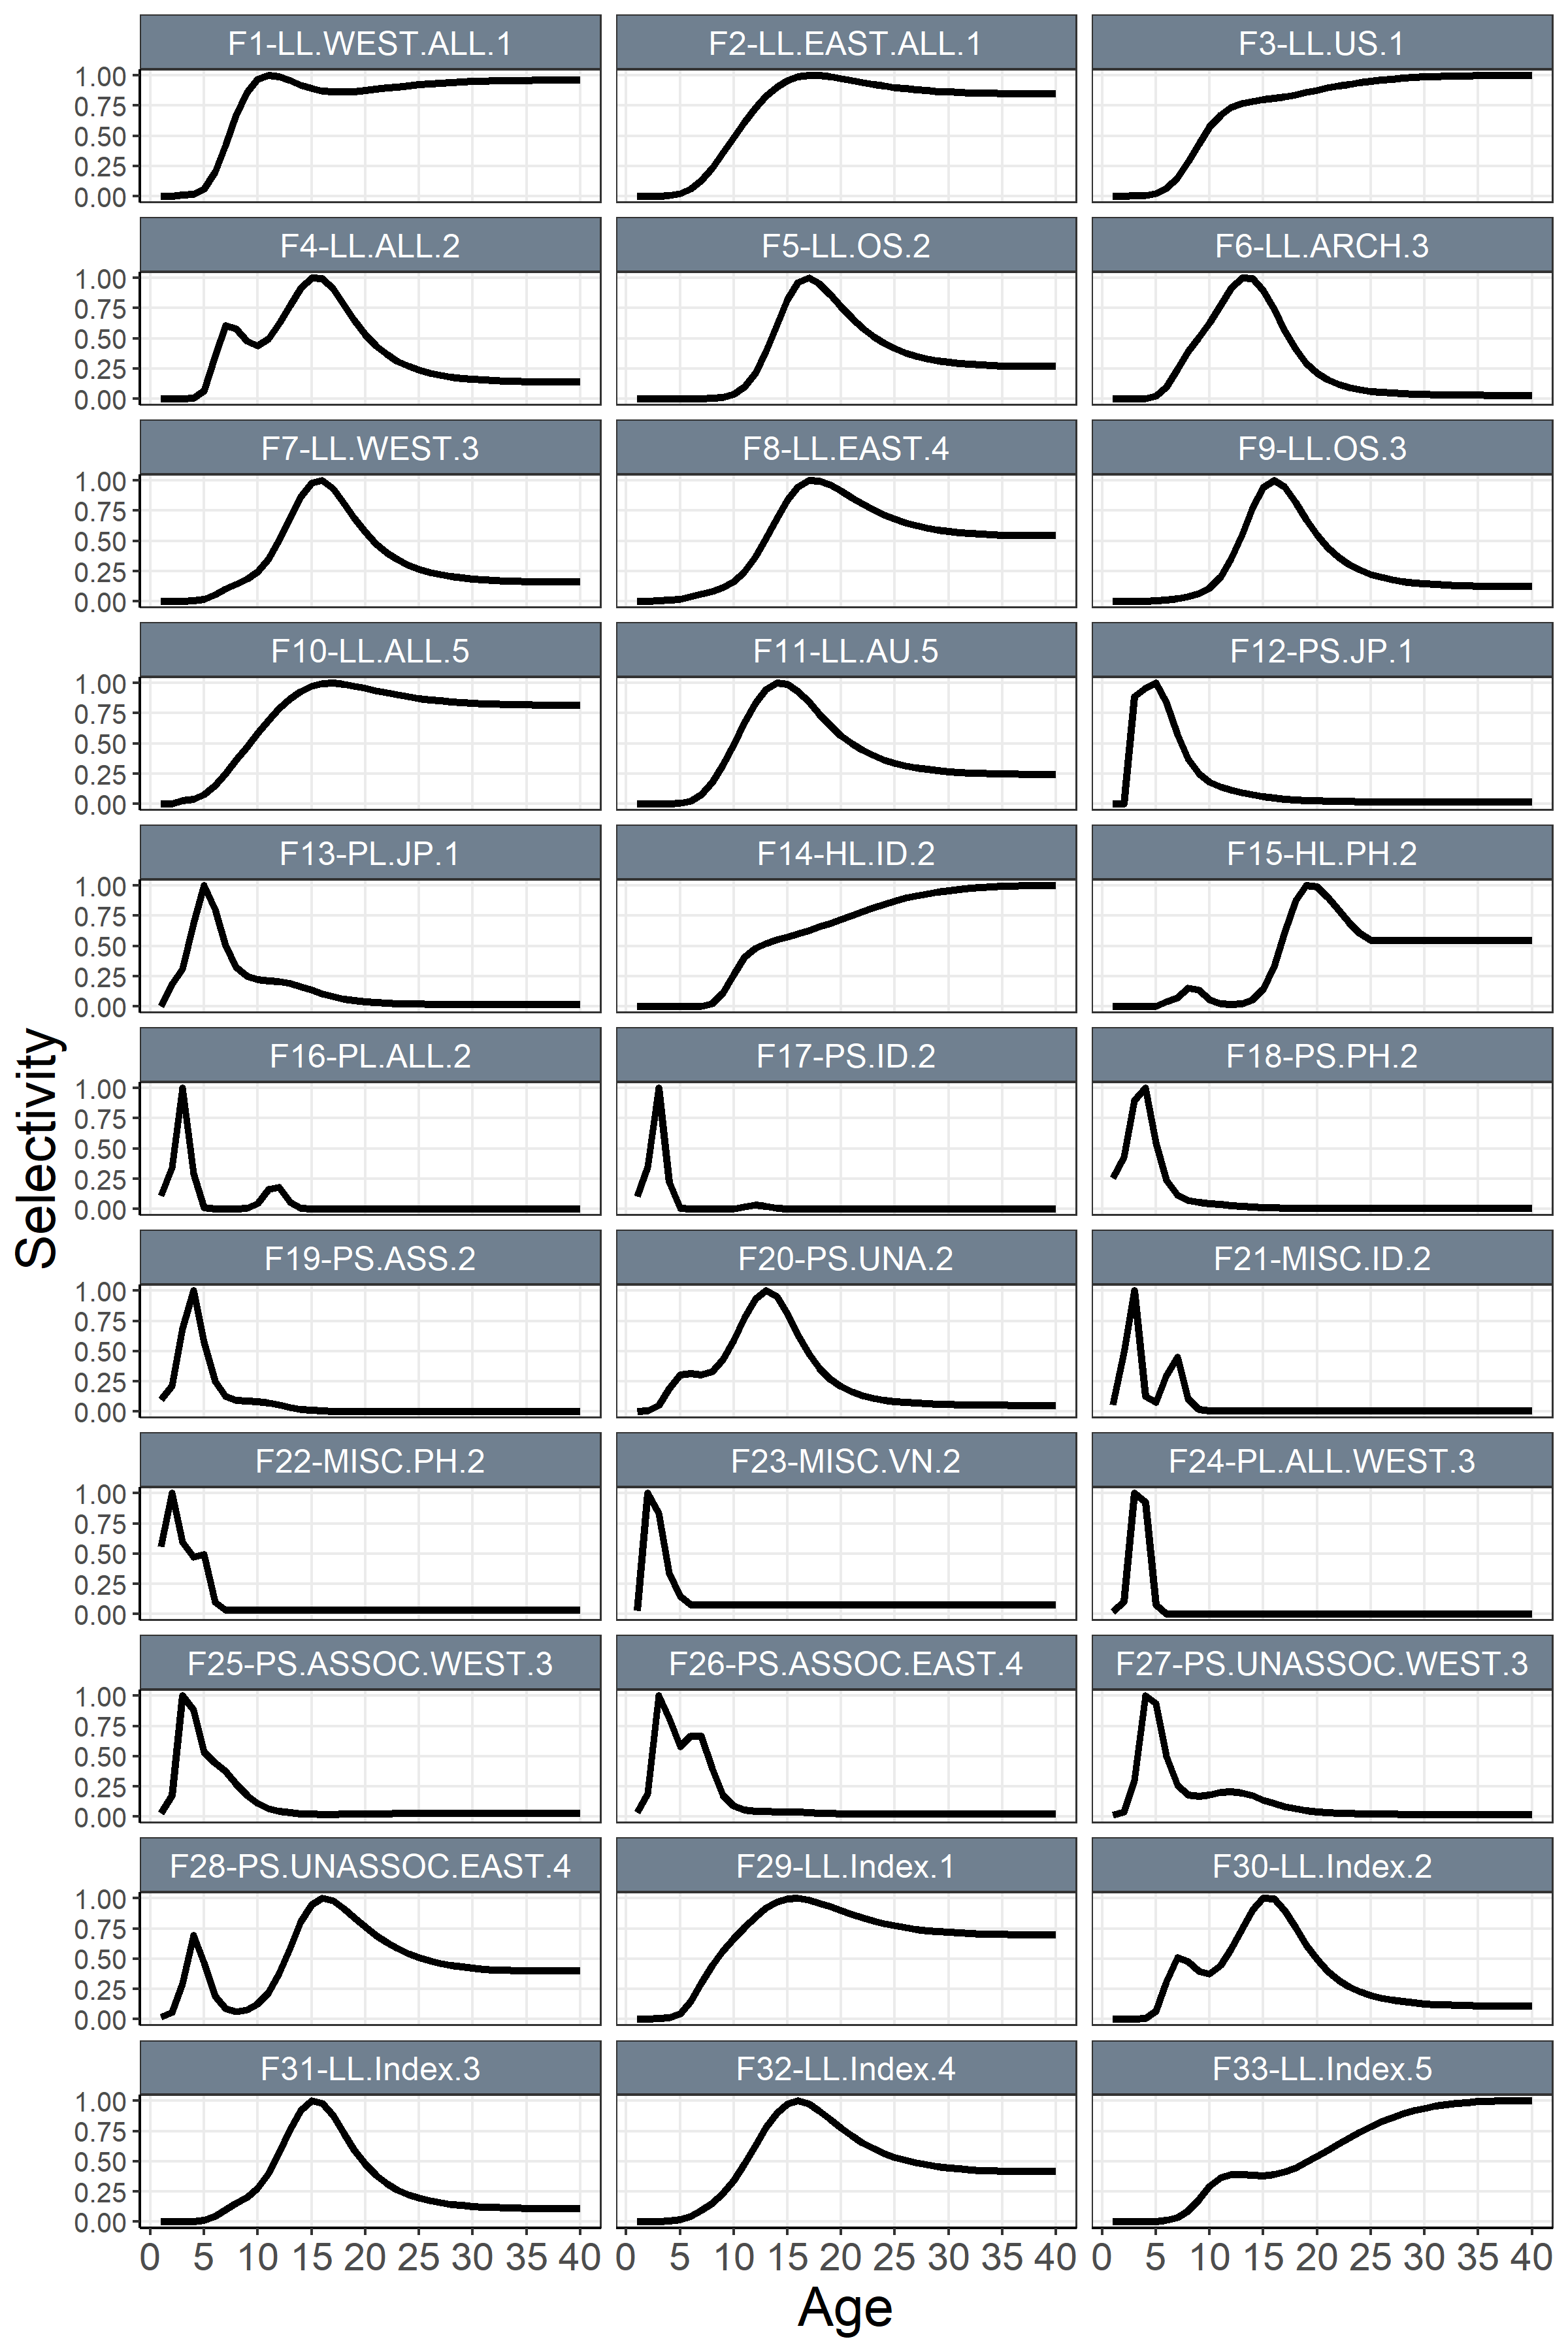
\includegraphics[width=0.8\linewidth,height=\textheight,keepaspectratio]{figures/select_age.png}
%DIFDELCMD <

%DIFDELCMD < }
%DIFDELCMD <

%DIFDELCMD < \caption{\label{fig-select-age}Age-specific (quarters) selectivity
%DIFDELCMD < curves for all extraction and index fisheries.}
%DIFDELCMD <

%DIFDELCMD < \end{figure}%%%
\DIFdelend \DIFaddbegin \begin{figure}[H]

\centering{

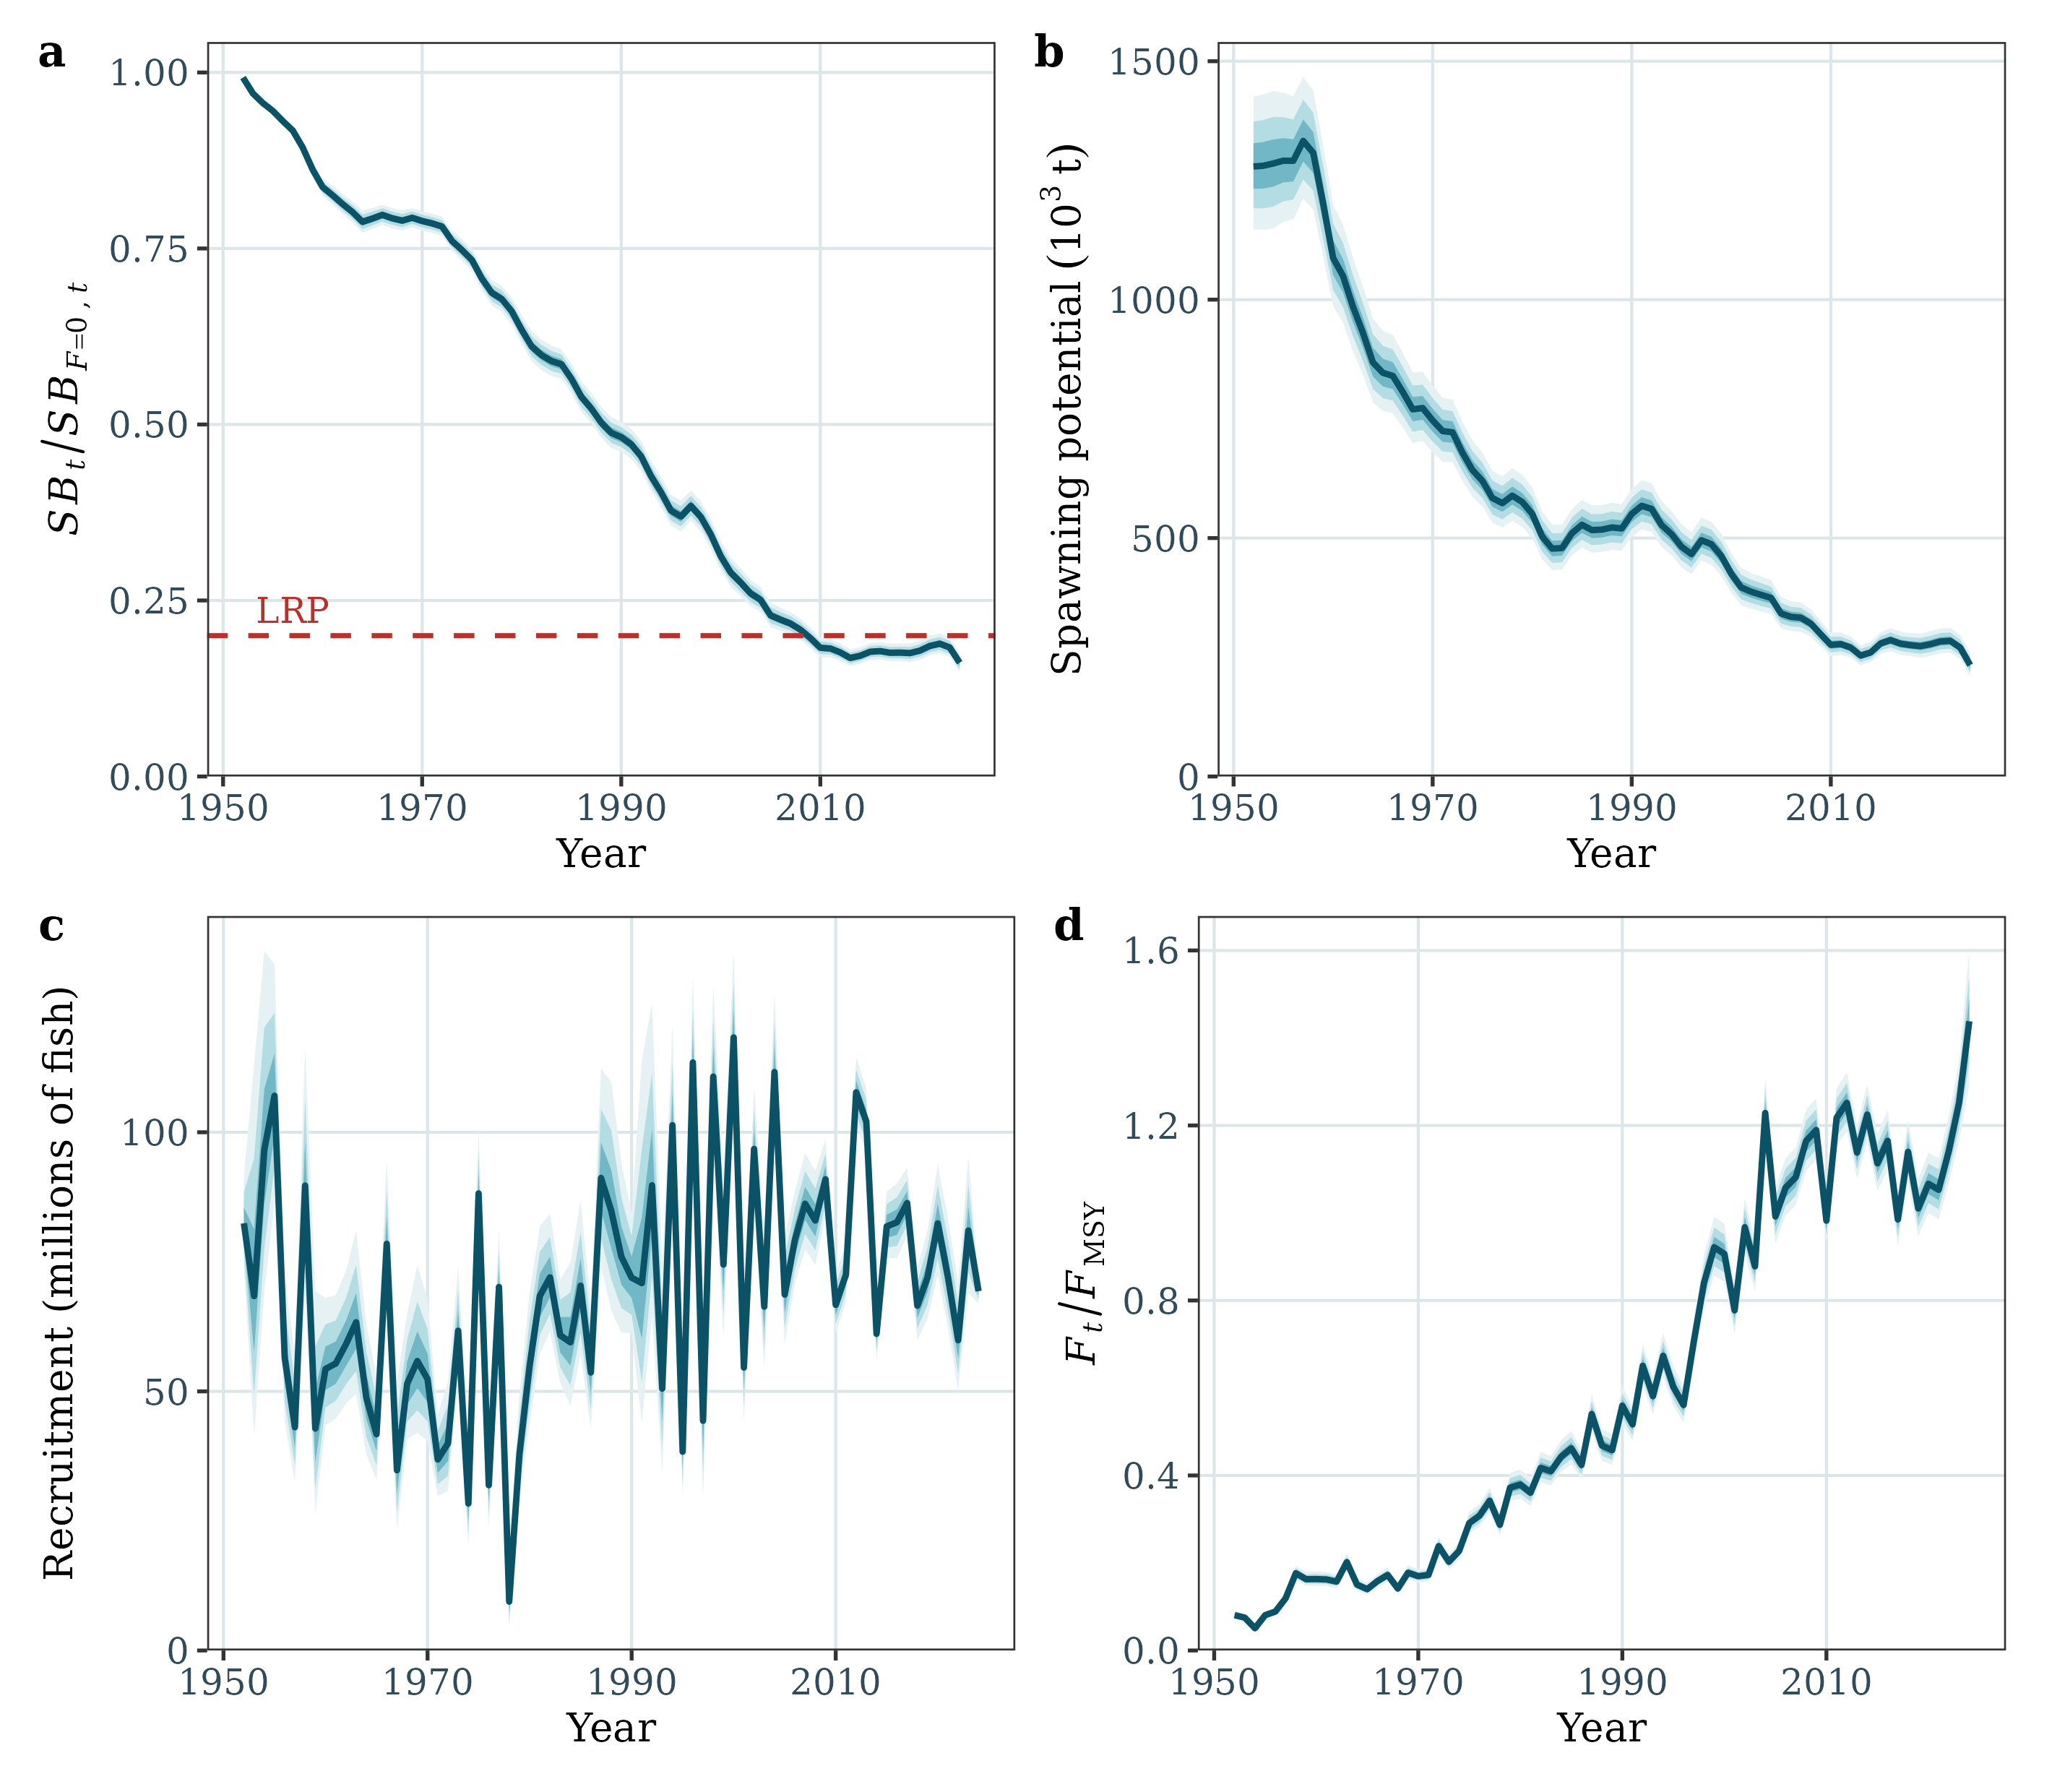
\includegraphics[width=1\linewidth,height=\textheight,keepaspectratio]{figures_new/diagnostic-population-dynamics.png}

}

\caption{\label{fig-diag-time-series}Diagnostic-model estimates of (a)
dynamic spawning depletion, (b) spawning potential, (c) recruitment and
(d) annual fishing mortality relative to \(F_{MSY}\). Shading gives
central 50\%, 80\% and 95\% Hessian delta-method intervals.}

\end{figure}\DIFaddend %

\DIFdelbegin %DIFDELCMD < \begin{figure}[H]
%DIFDELCMD <

%DIFDELCMD < \centering{
%DIFDELCMD <

%DIFDELCMD < 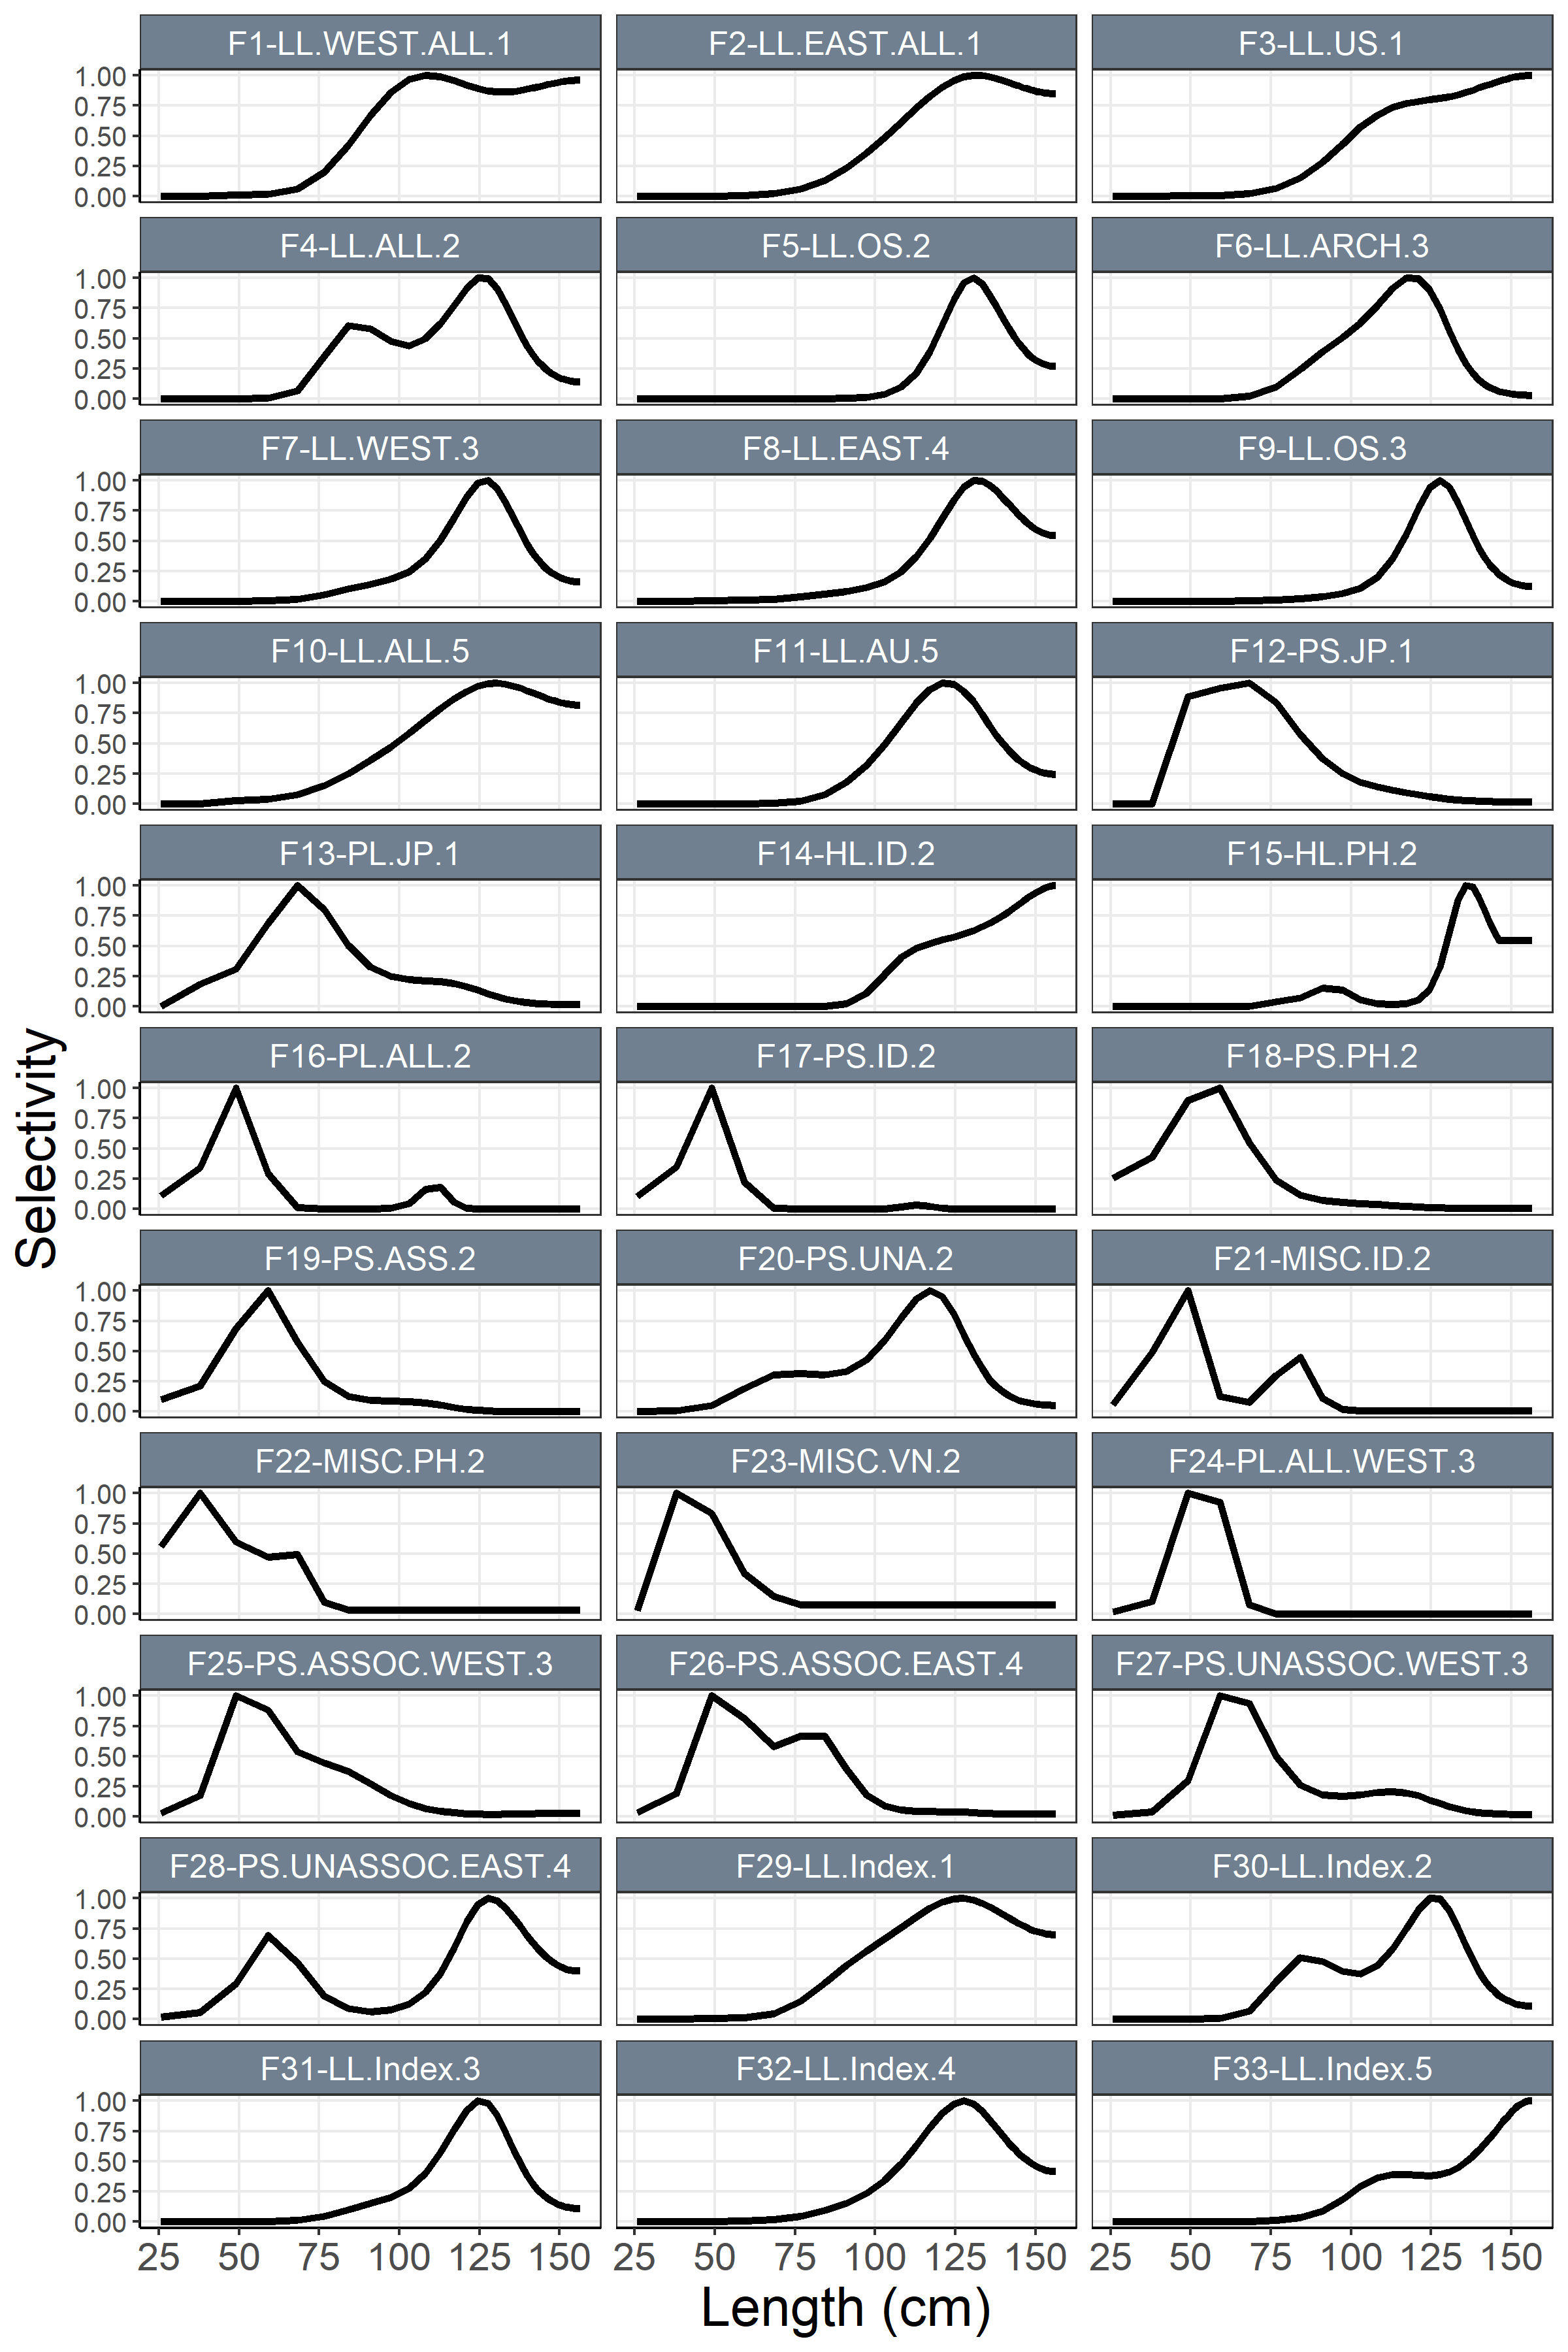
\includegraphics[width=0.8\linewidth,height=\textheight,keepaspectratio]{figures/select_length.png}
%DIFDELCMD <

%DIFDELCMD < }
%DIFDELCMD <

%DIFDELCMD < \caption{\label{fig-select-length}Length (cm) selectivity curves for all
%DIFDELCMD < extraction and index fisheries.}
%DIFDELCMD <

%DIFDELCMD < \end{figure}%%%
\DIFdelend \DIFaddbegin \begin{figure}[H]

\centering{

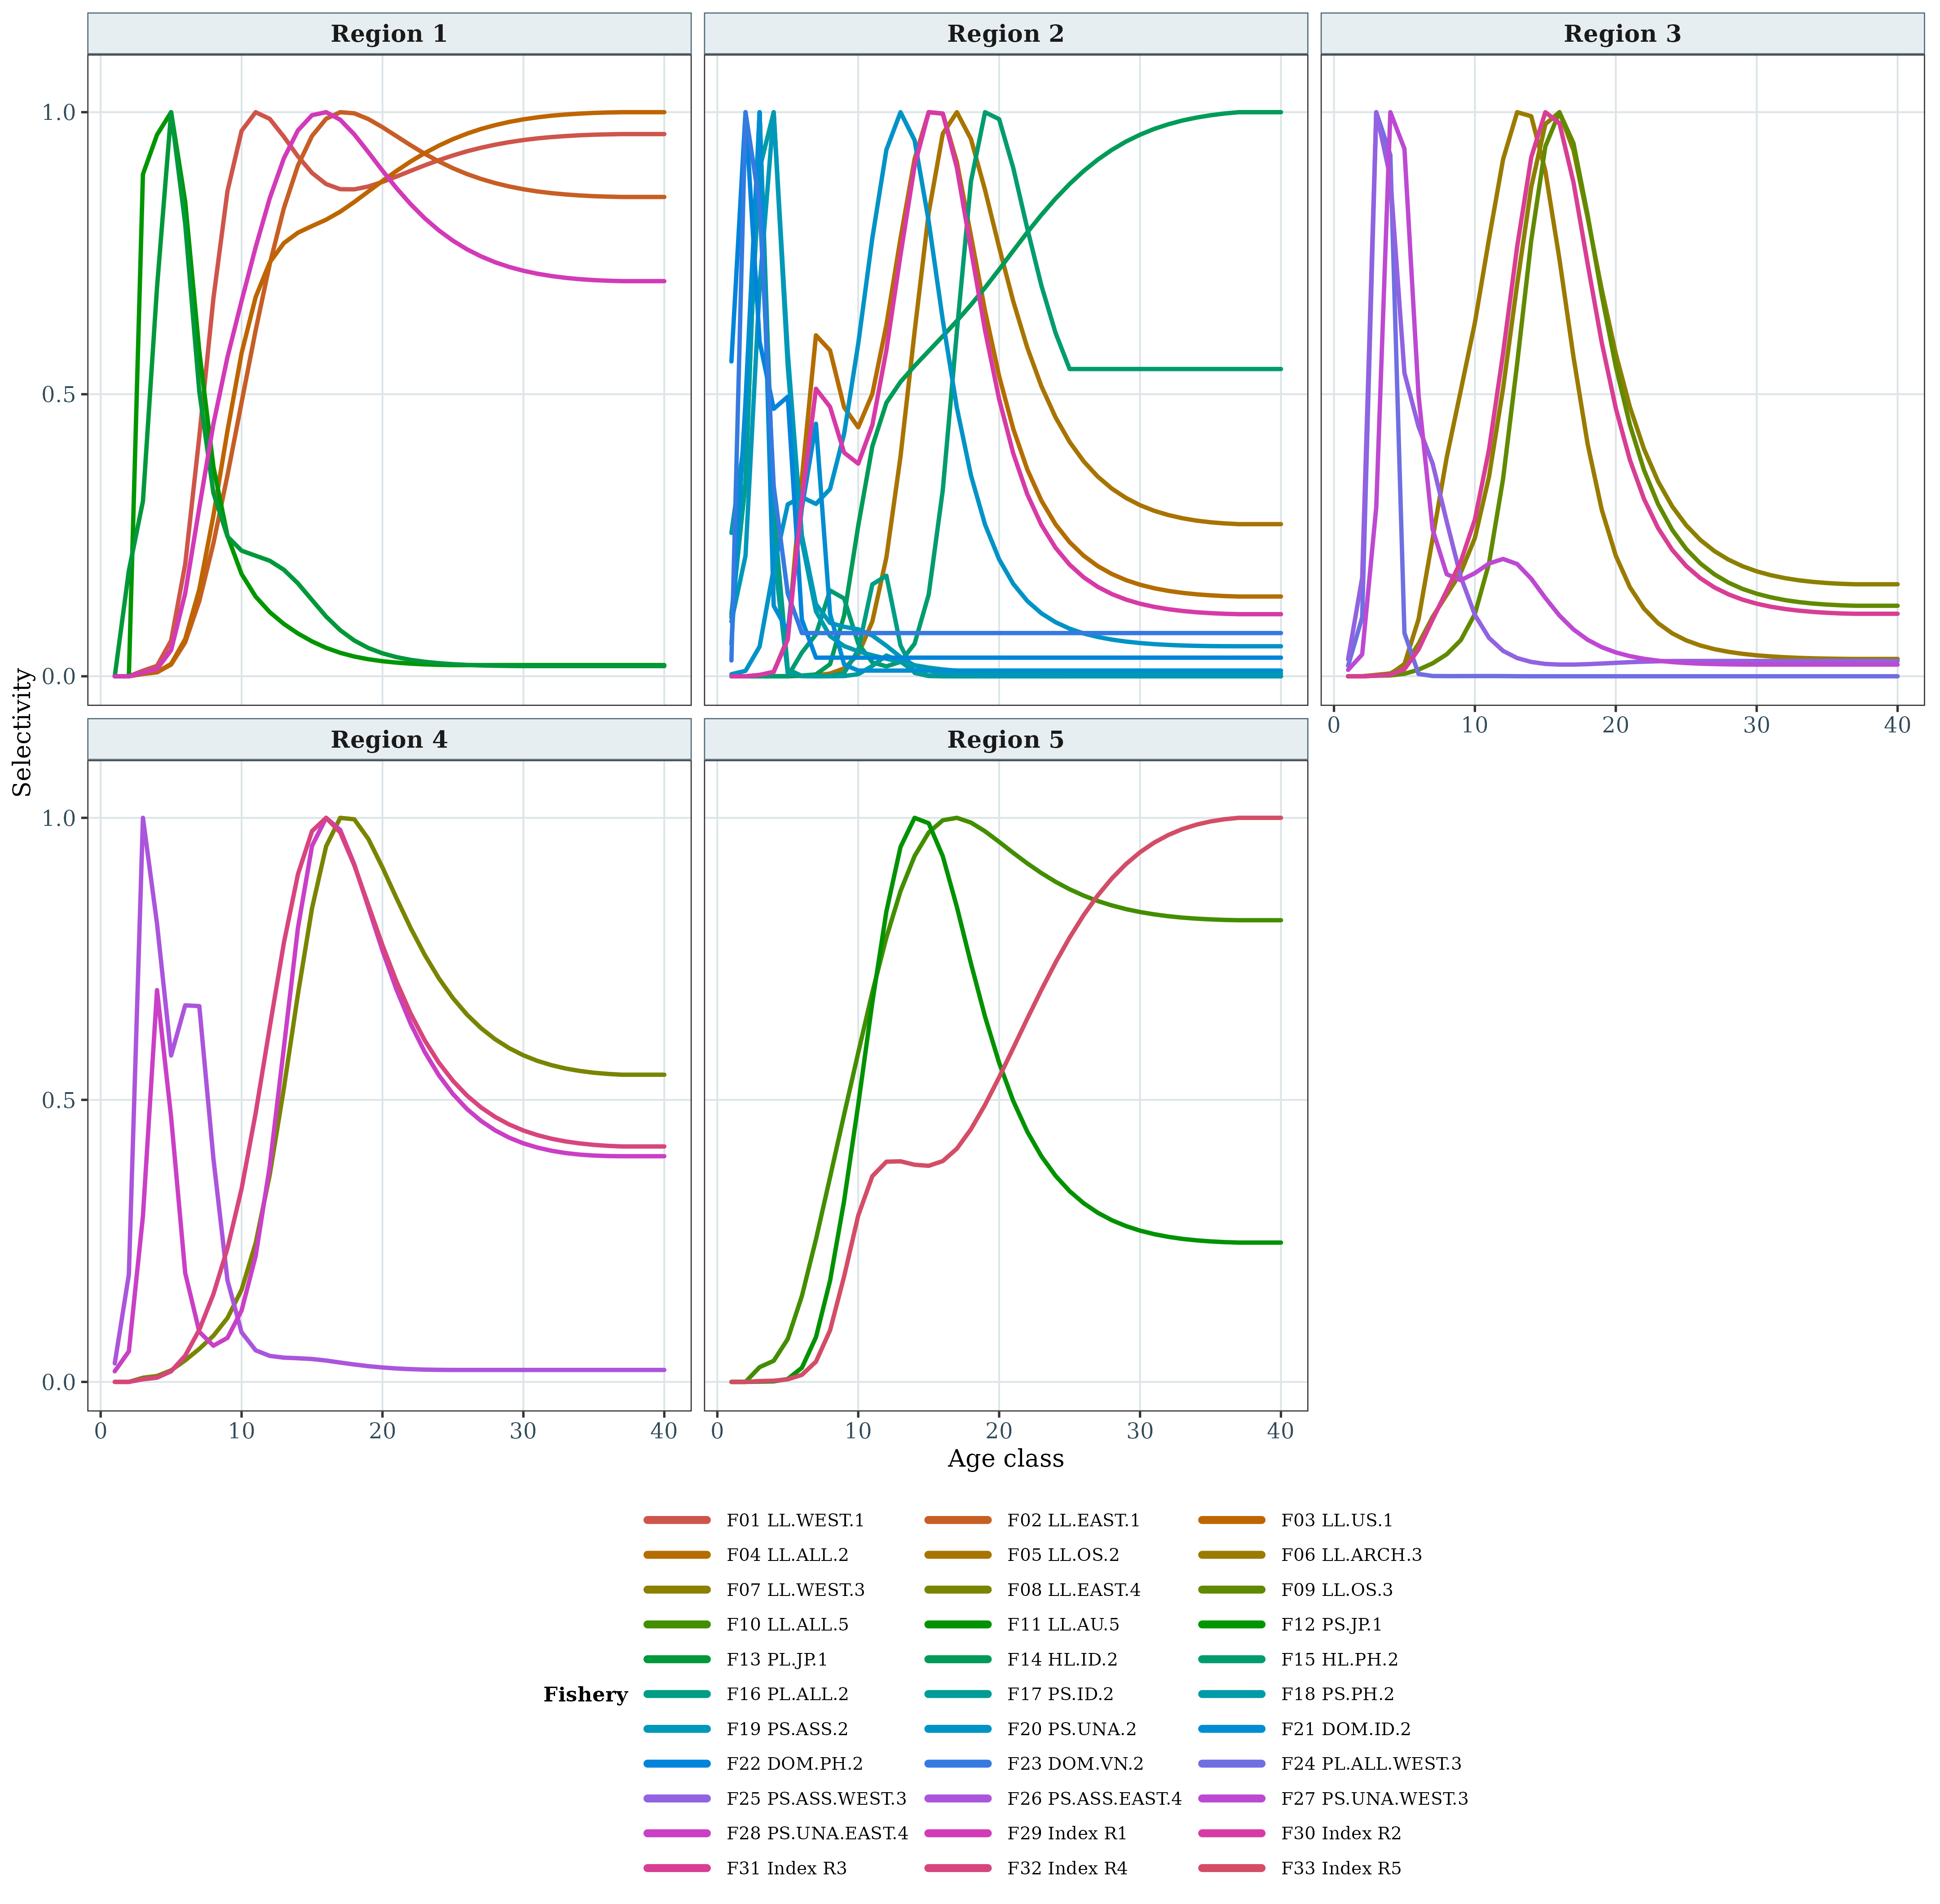
\includegraphics[width=1\linewidth,height=\textheight,keepaspectratio]{figures_new/fishery-process.png}

}

\caption{\label{fig-select-age}Estimated fishery selectivity at age for
all 33 fisheries, grouped into the five model-region panels. Colours and
the complete fishery key identify each fitted cubic-spline curve.}

\end{figure}\DIFaddend %

\DIFdelbegin %DIFDELCMD < \begin{figure}[H]
%DIFDELCMD <

%DIFDELCMD < \centering{
%DIFDELCMD <

%DIFDELCMD < 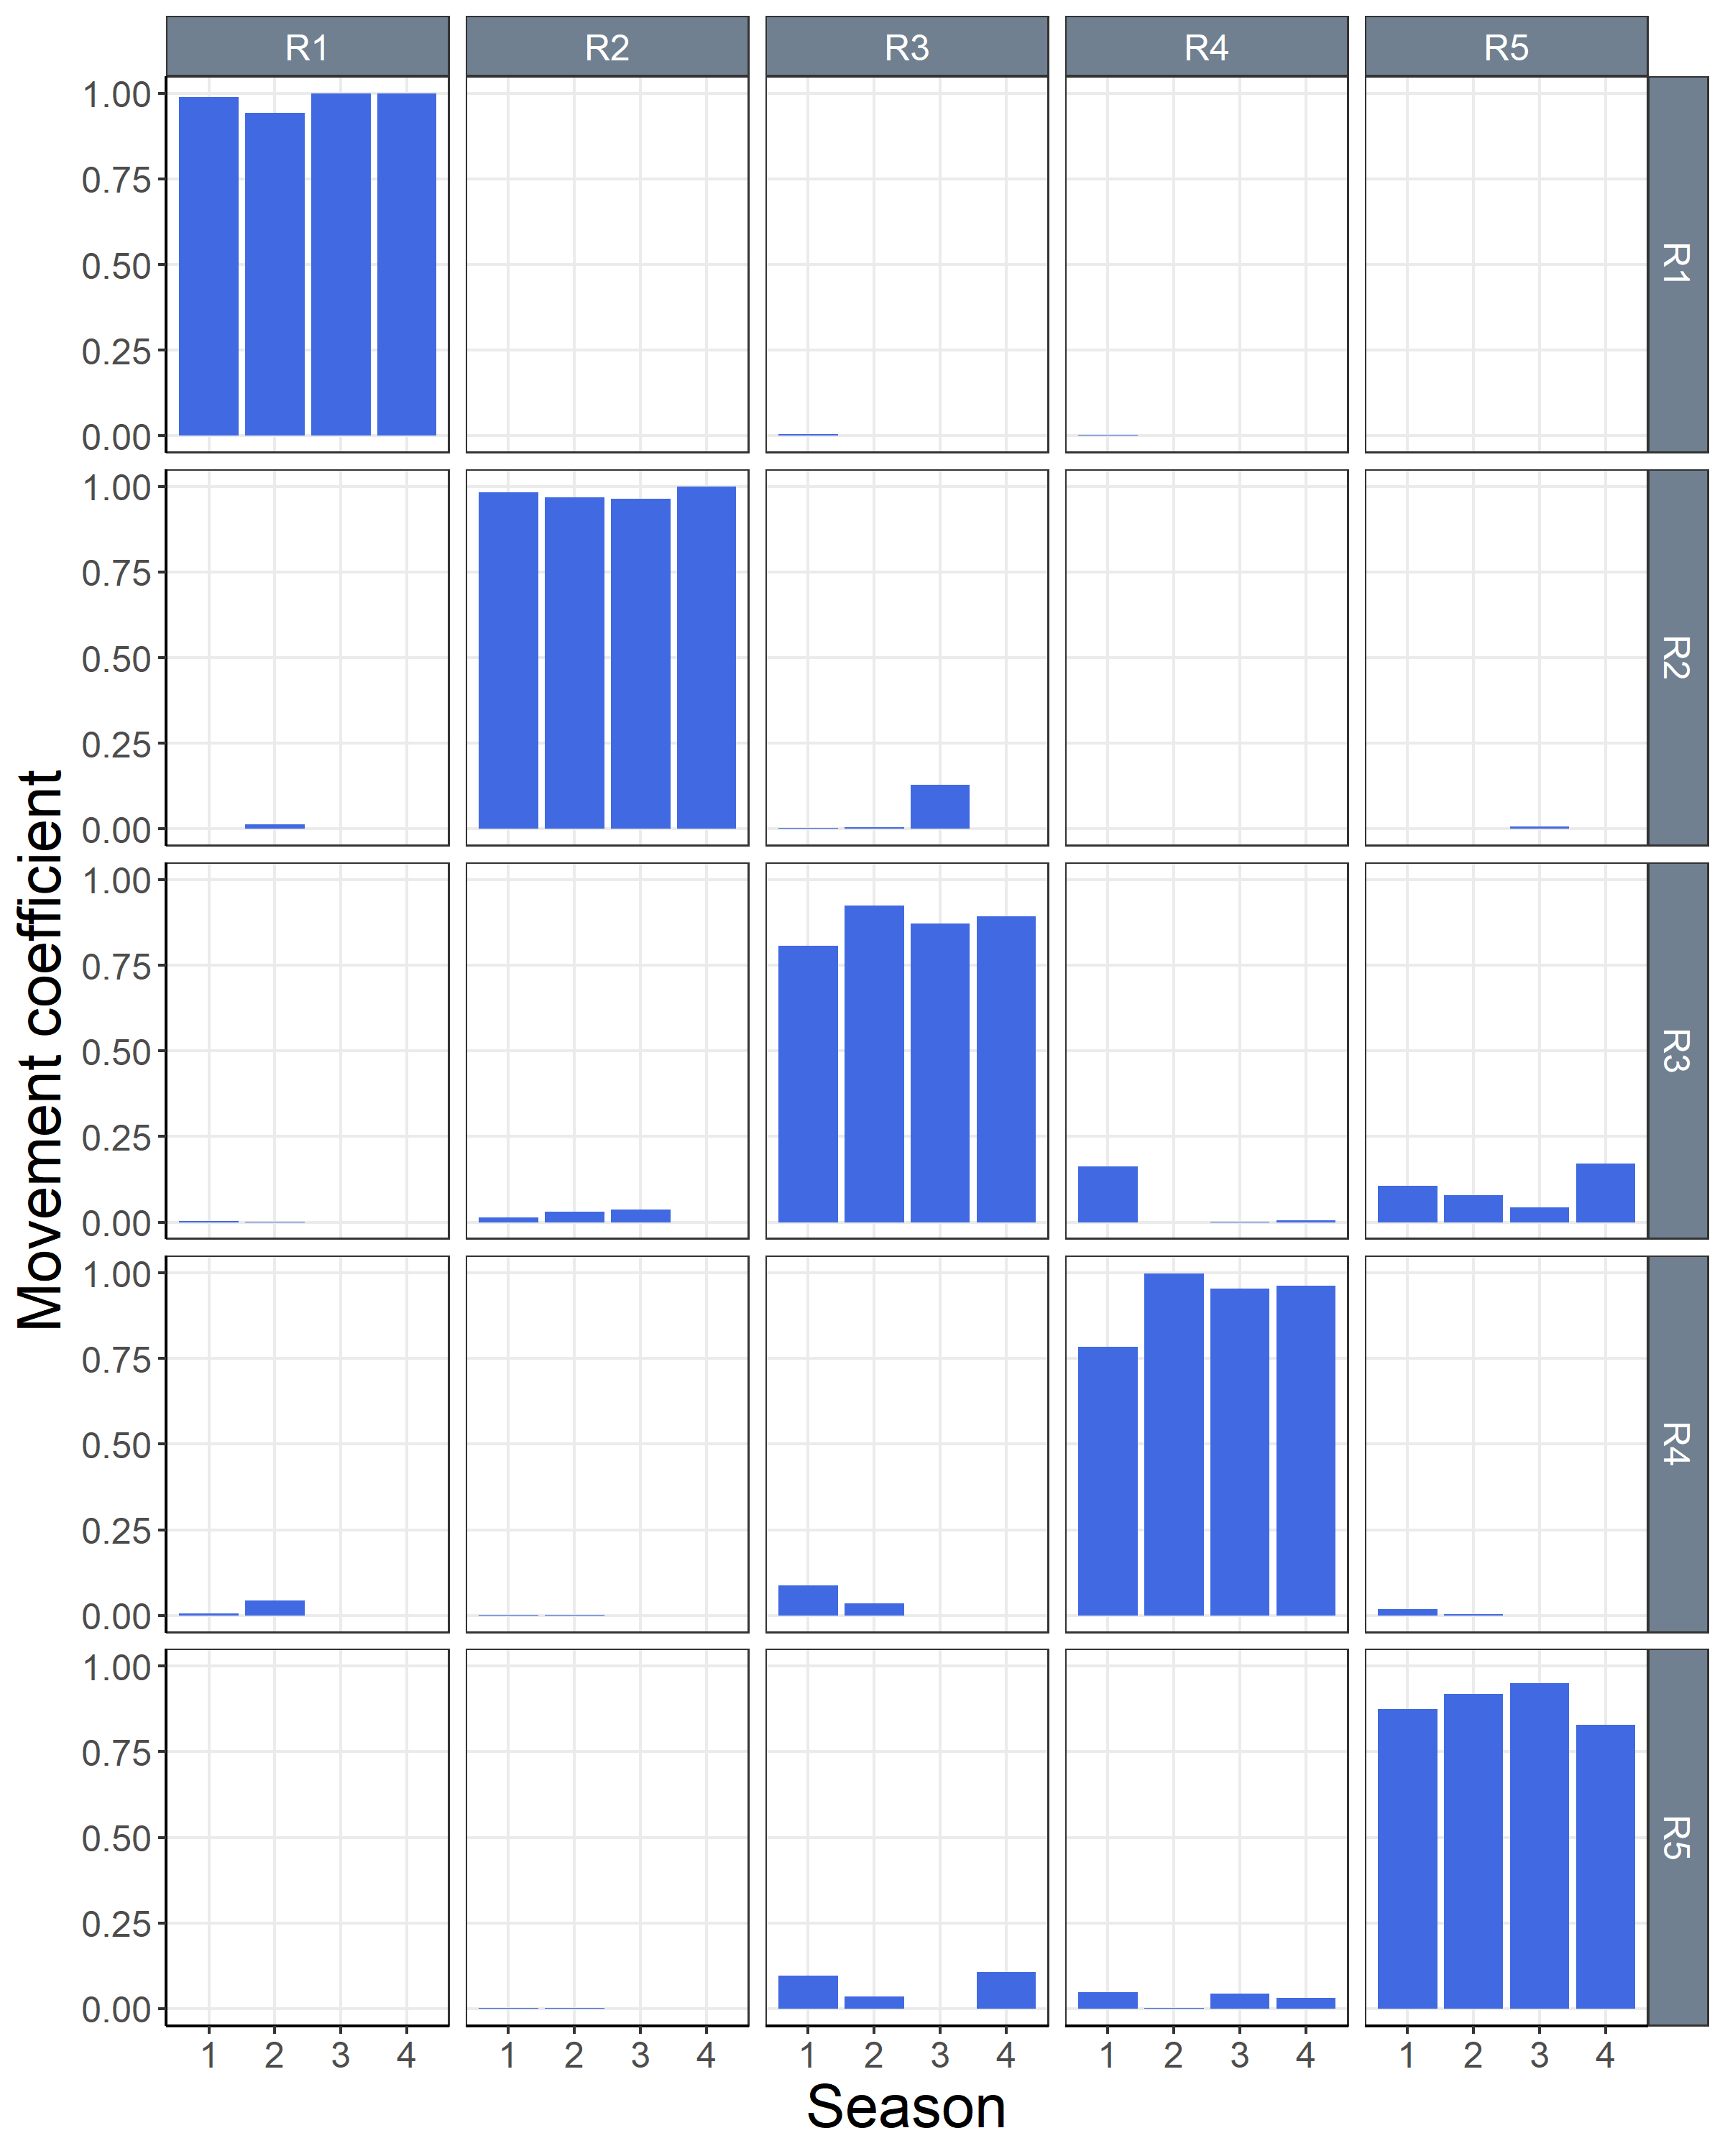
\includegraphics[width=1\linewidth,height=\textheight,keepaspectratio]{figures/movement_bar_plots.png}
%DIFDELCMD <

%DIFDELCMD < }
%DIFDELCMD <

%DIFDELCMD < \caption{\label{fig-season-movement-coeff}Season-specific movement
%DIFDELCMD < probabilities among model regions estimated by the 2026 diagnostic
%DIFDELCMD < model.}
%DIFDELCMD <

%DIFDELCMD < \end{figure}%%%
\DIFdelend \DIFaddbegin \begin{figure}[H]

\centering{

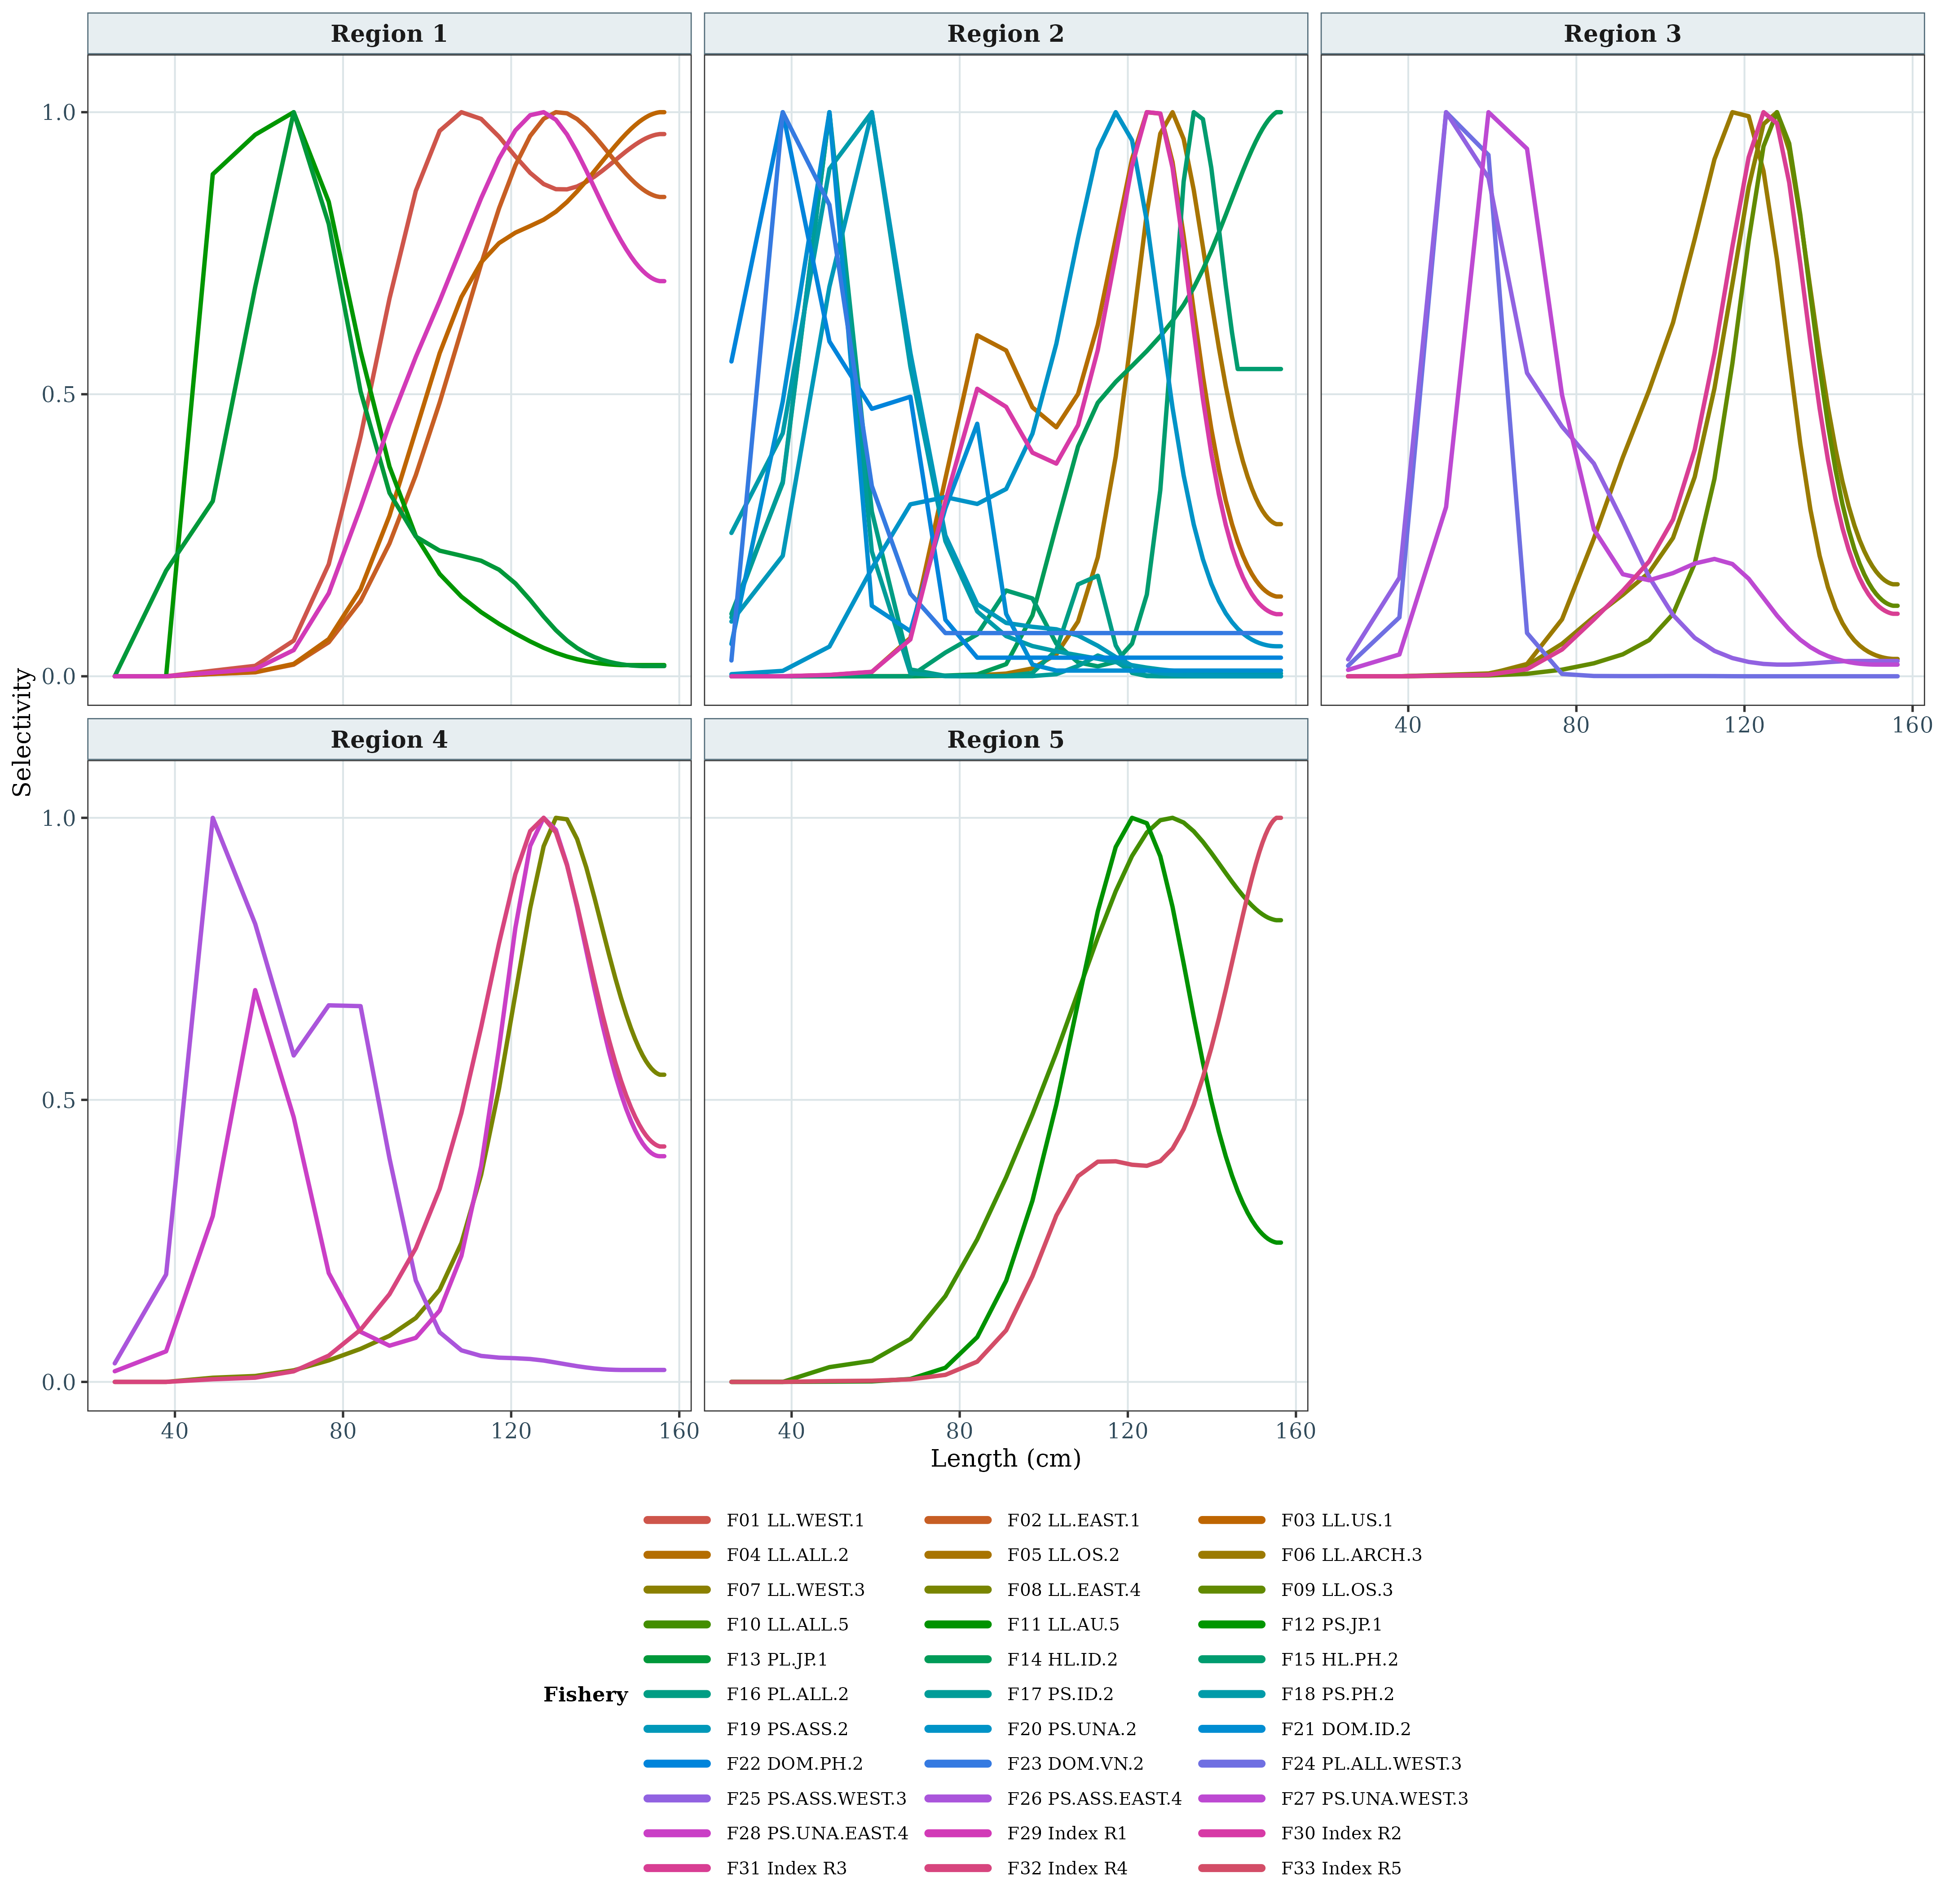
\includegraphics[width=1\linewidth,height=\textheight,keepaspectratio]{figures_new/fishery-selectivity-length.png}

}

\caption{\label{fig-select-length}Estimated fishery selectivity at
length for all 33 fisheries, grouped into the five model-region panels.
Length is the fitted mean length at each age class.}

\end{figure}\DIFaddend %

\DIFdelbegin %DIFDELCMD < \begin{figure}[H]
%DIFDELCMD <

%DIFDELCMD < \centering{
%DIFDELCMD <

%DIFDELCMD < 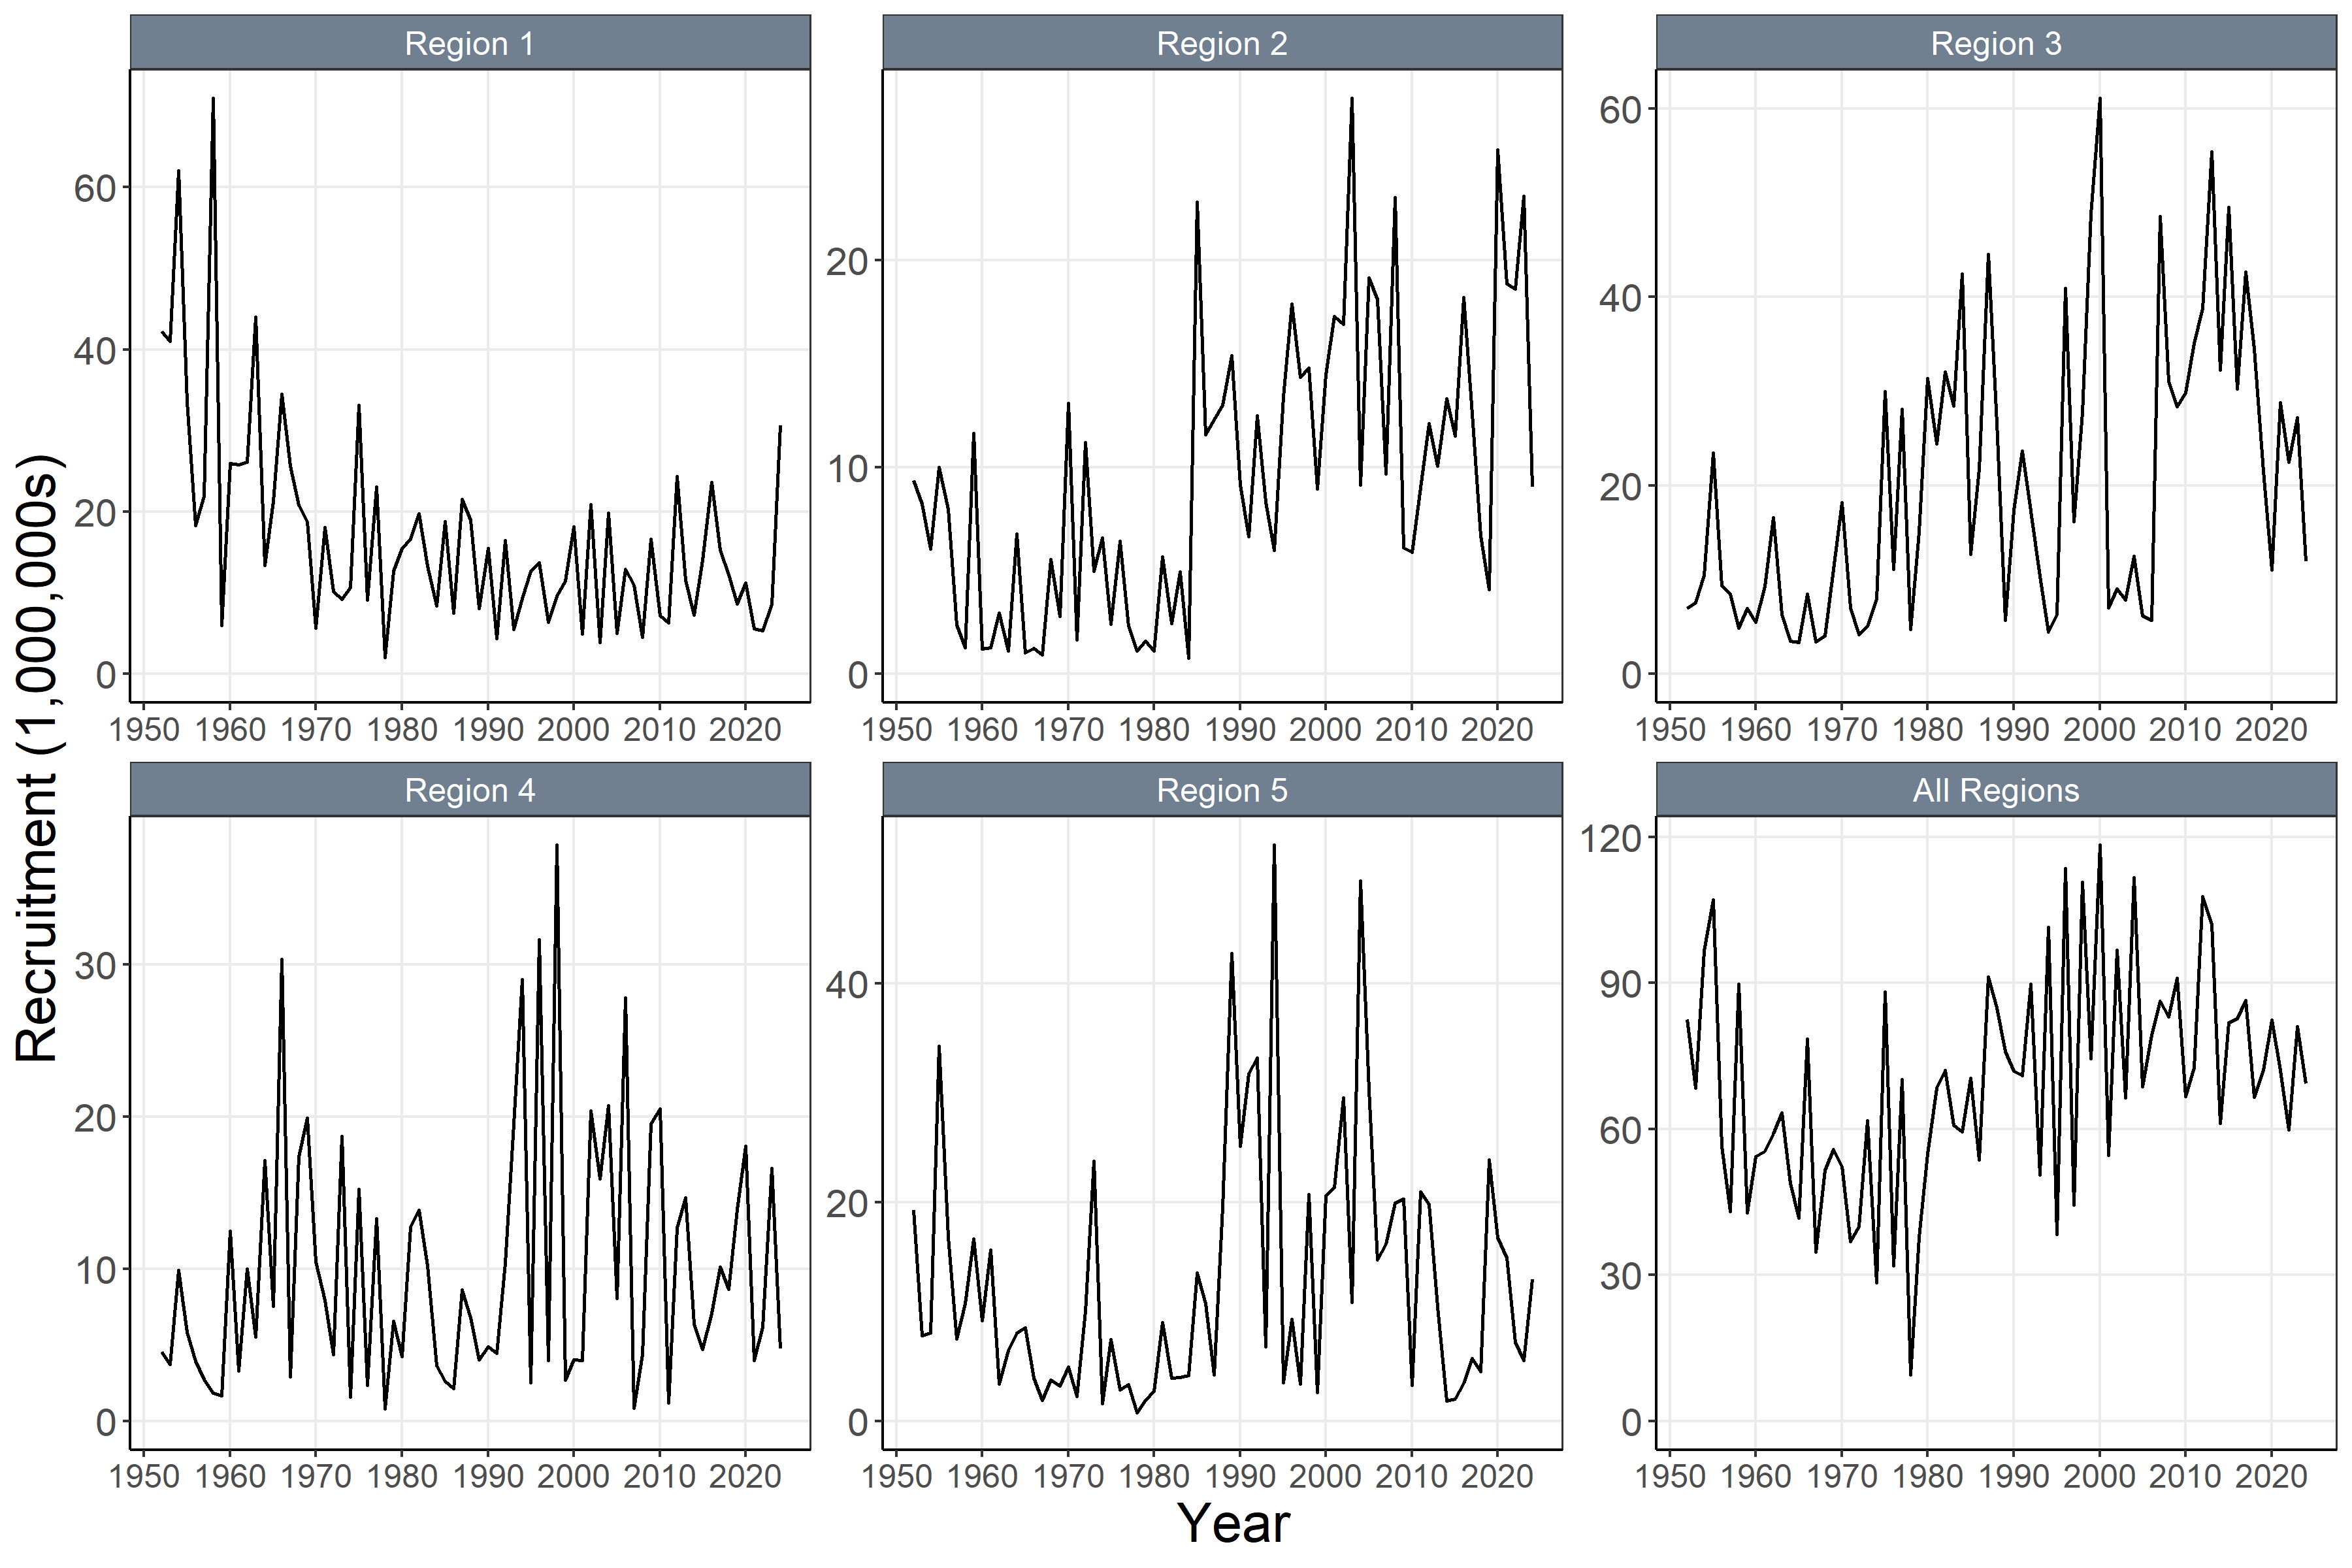
\includegraphics[width=1\linewidth,height=\textheight,keepaspectratio]{figures/recruitment_annual.png}
%DIFDELCMD <

%DIFDELCMD < }
%DIFDELCMD <

%DIFDELCMD < \caption{\label{fig-recruitment-annual}Time series of estimated total
%DIFDELCMD < annual recruitment summed across regions (all) and for each model region
%DIFDELCMD < for the 2026 diagnostic model.}
%DIFDELCMD <

%DIFDELCMD < \end{figure}%%%
\DIFdelend \DIFaddbegin \begin{figure}[H]

\centering{

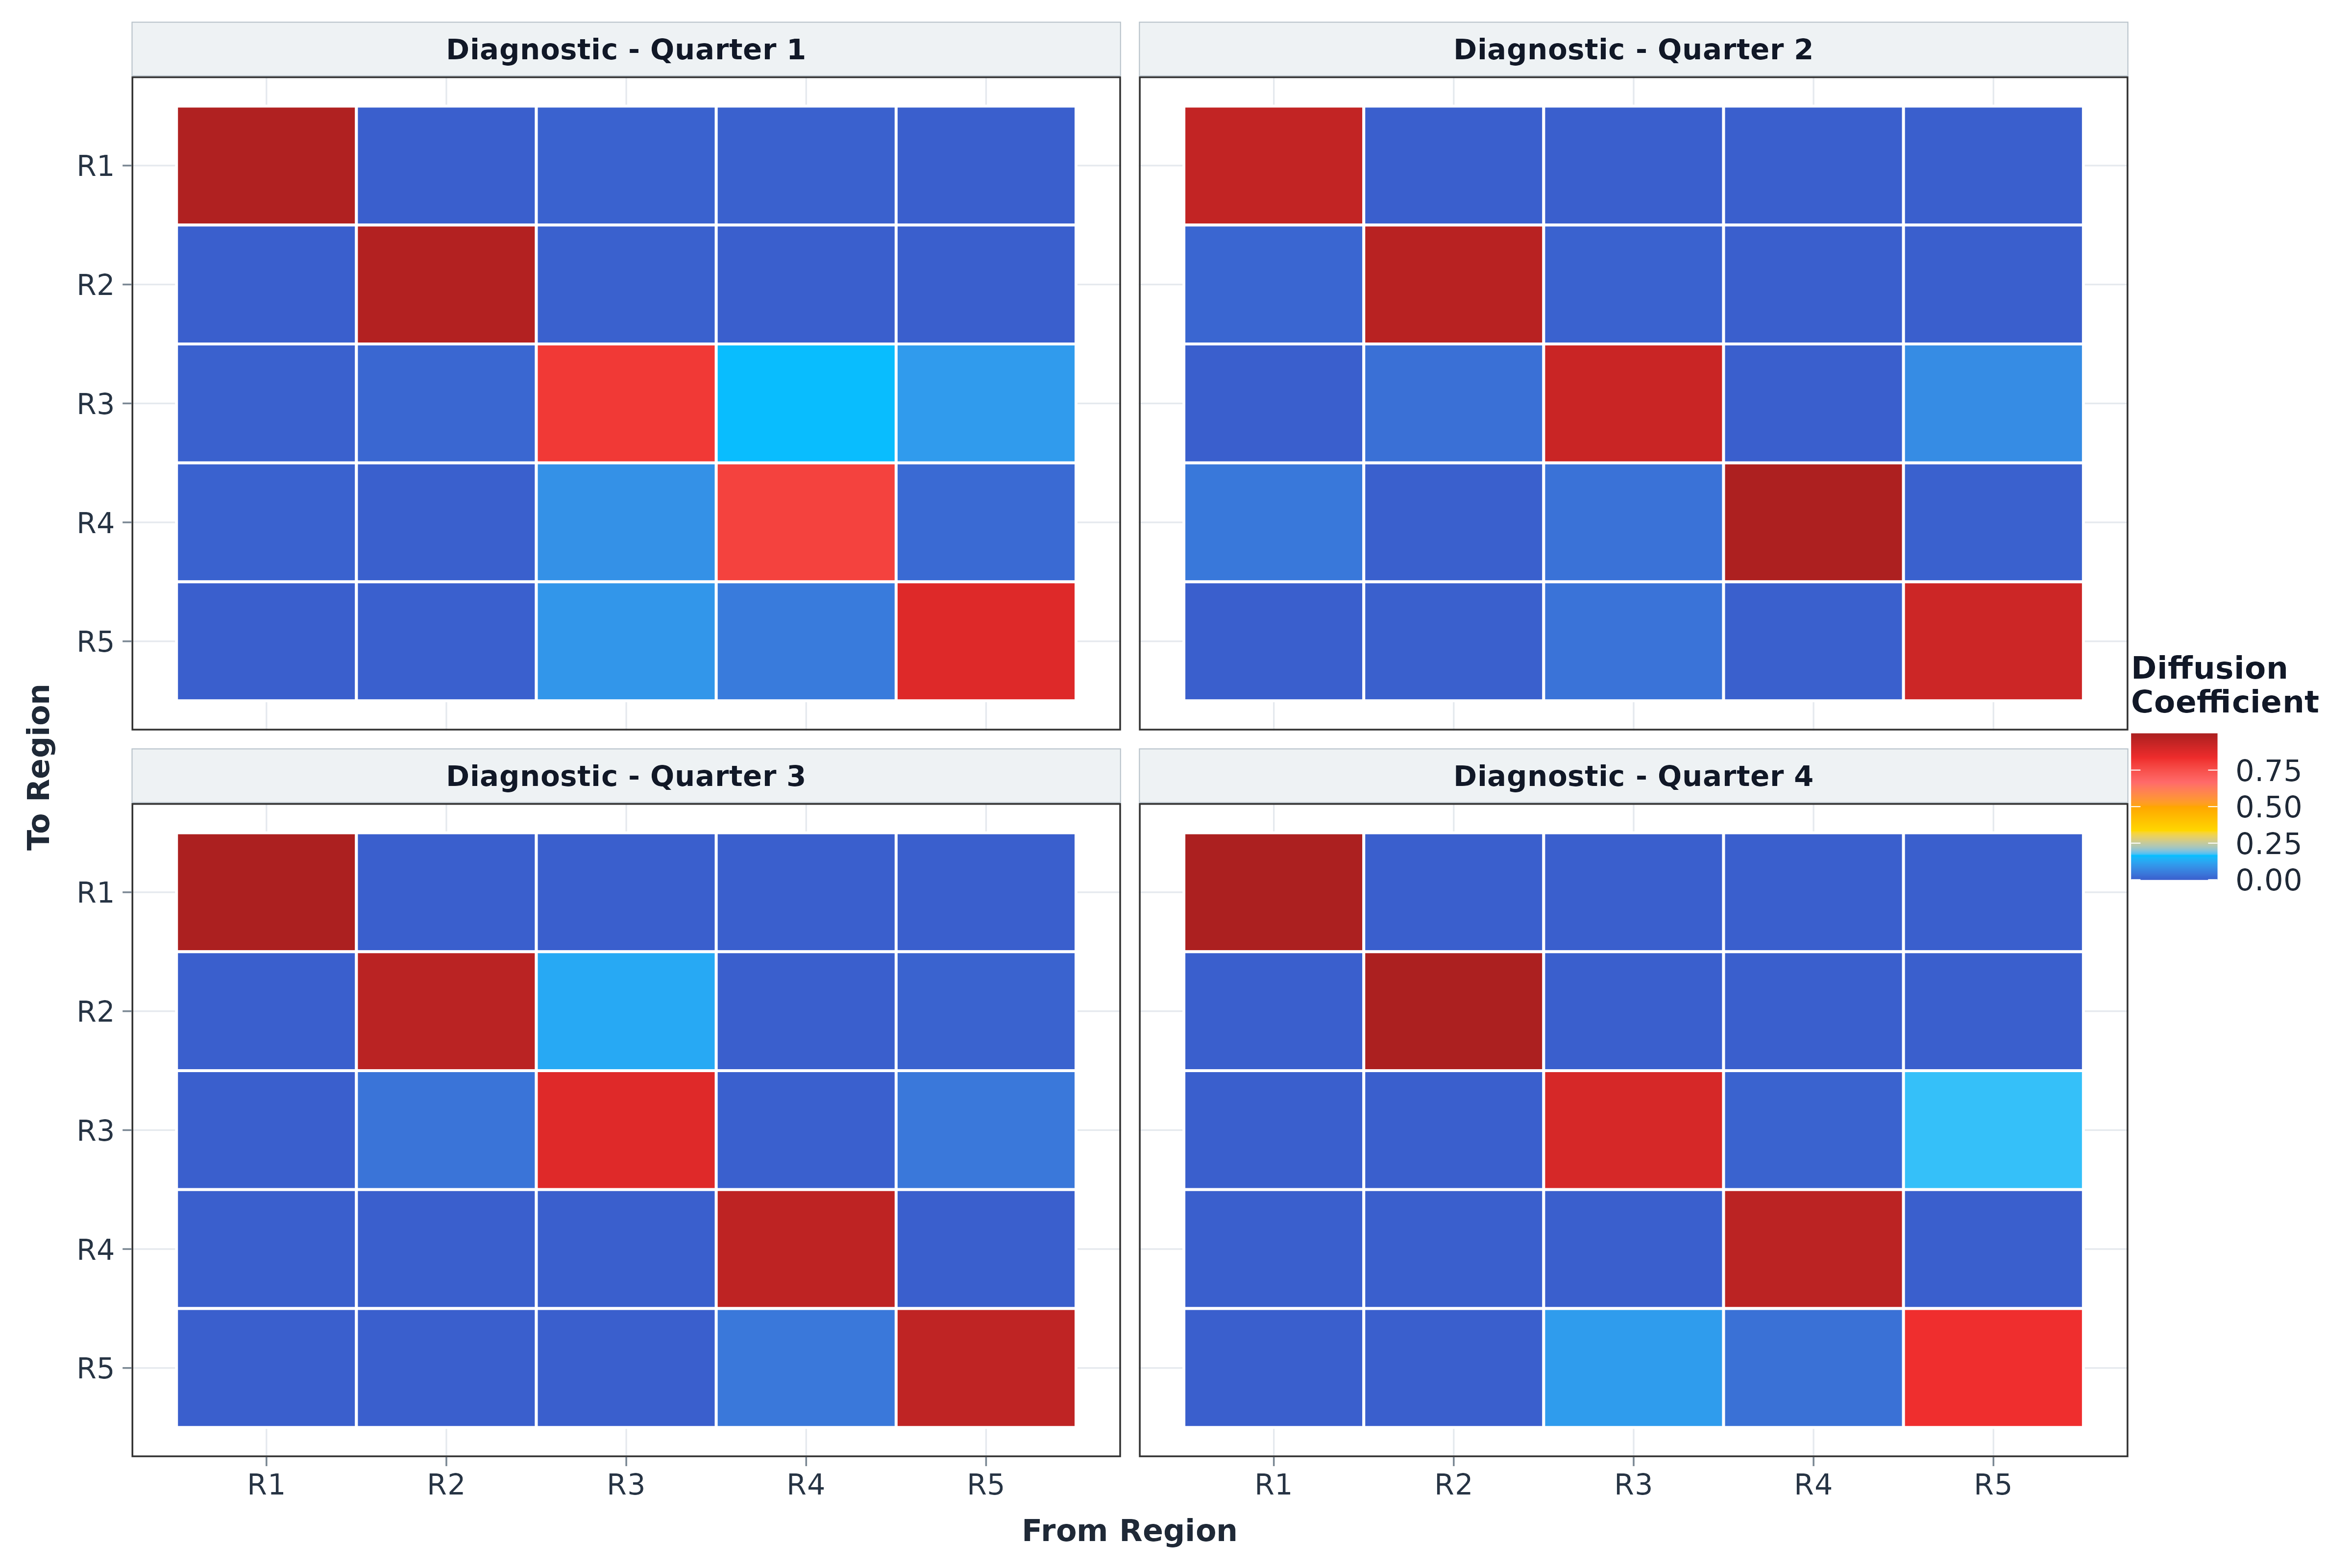
\includegraphics[width=1\linewidth,height=\textheight,keepaspectratio]{figures_new/regional-movement.png}

}

\caption{\label{fig-season-movement-coeff}Estimated quarterly movement
probabilities among the five model regions.}

\end{figure}%DIF >

\begin{figure}[H]

\centering{

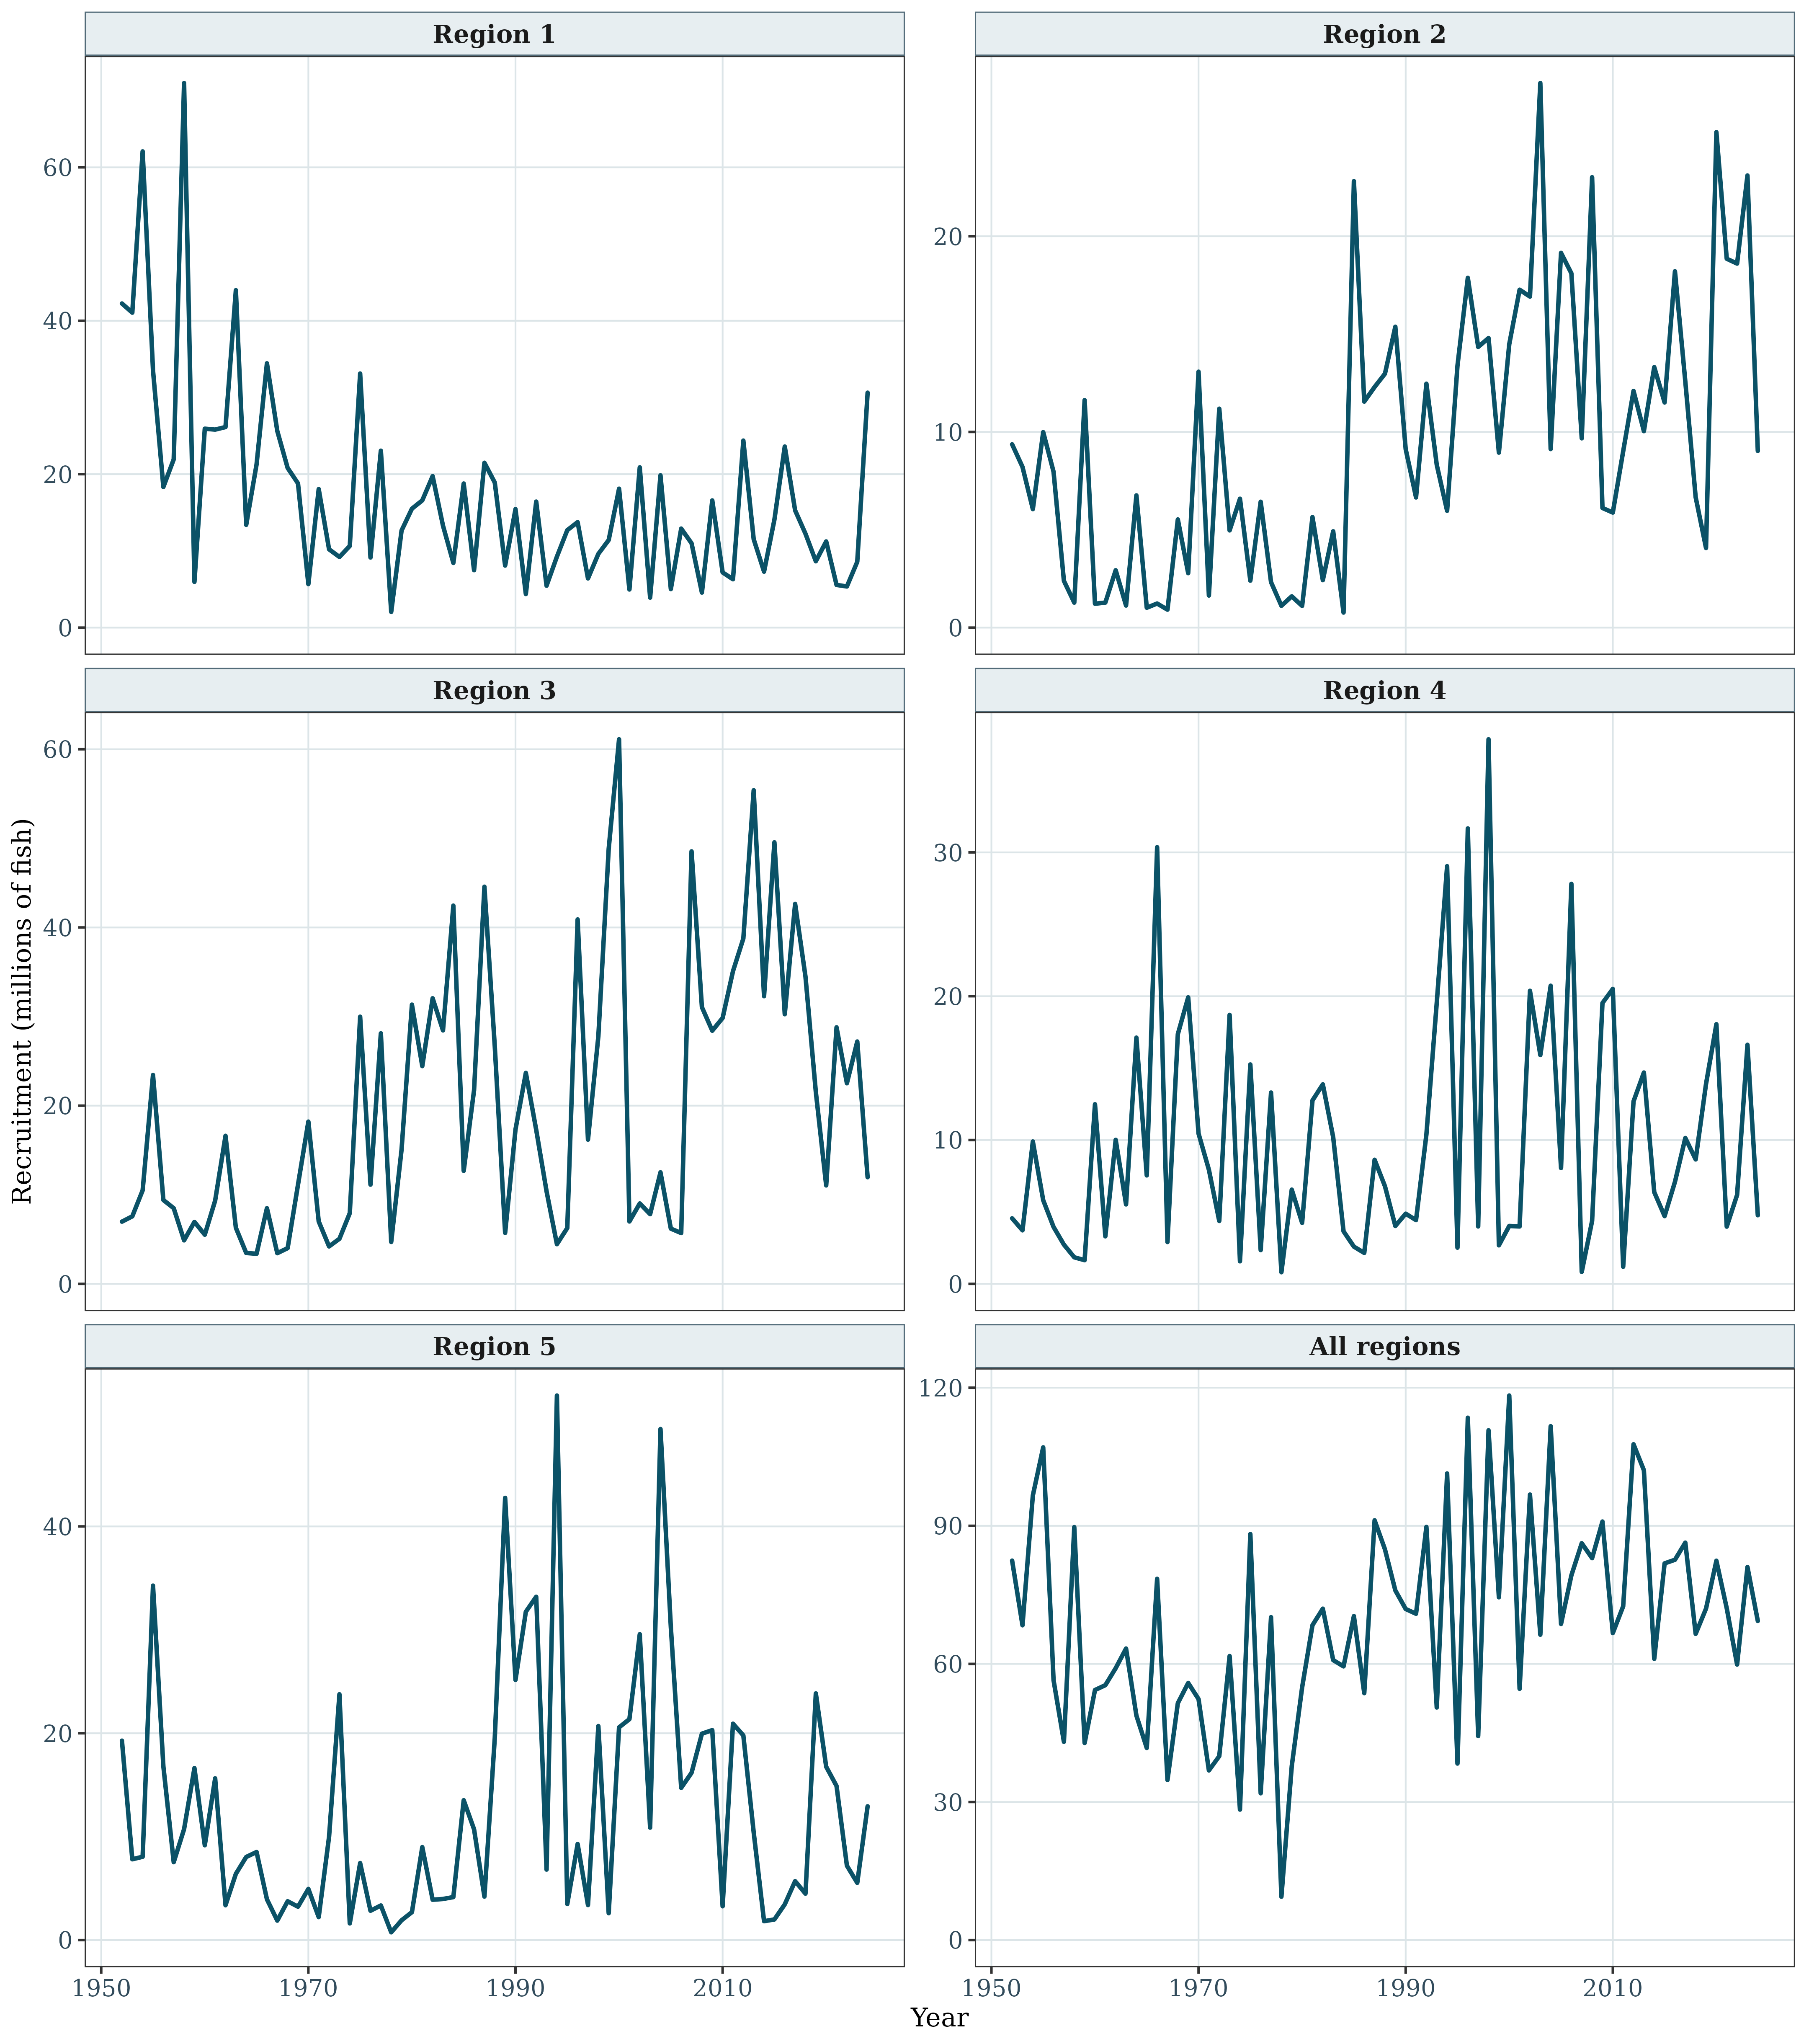
\includegraphics[width=1\linewidth,height=\textheight,keepaspectratio]{figures_new/recruitment-by-area-2col.png}

}

\caption{\label{fig-recruitment-annual}Estimated annual recruitment by
model region and the pooled All regions series (last). The two-column
layout provides additional panel height; panel y axes are free and begin
at zero.}

\end{figure}\DIFaddend %

\begin{figure}[H]

\centering{

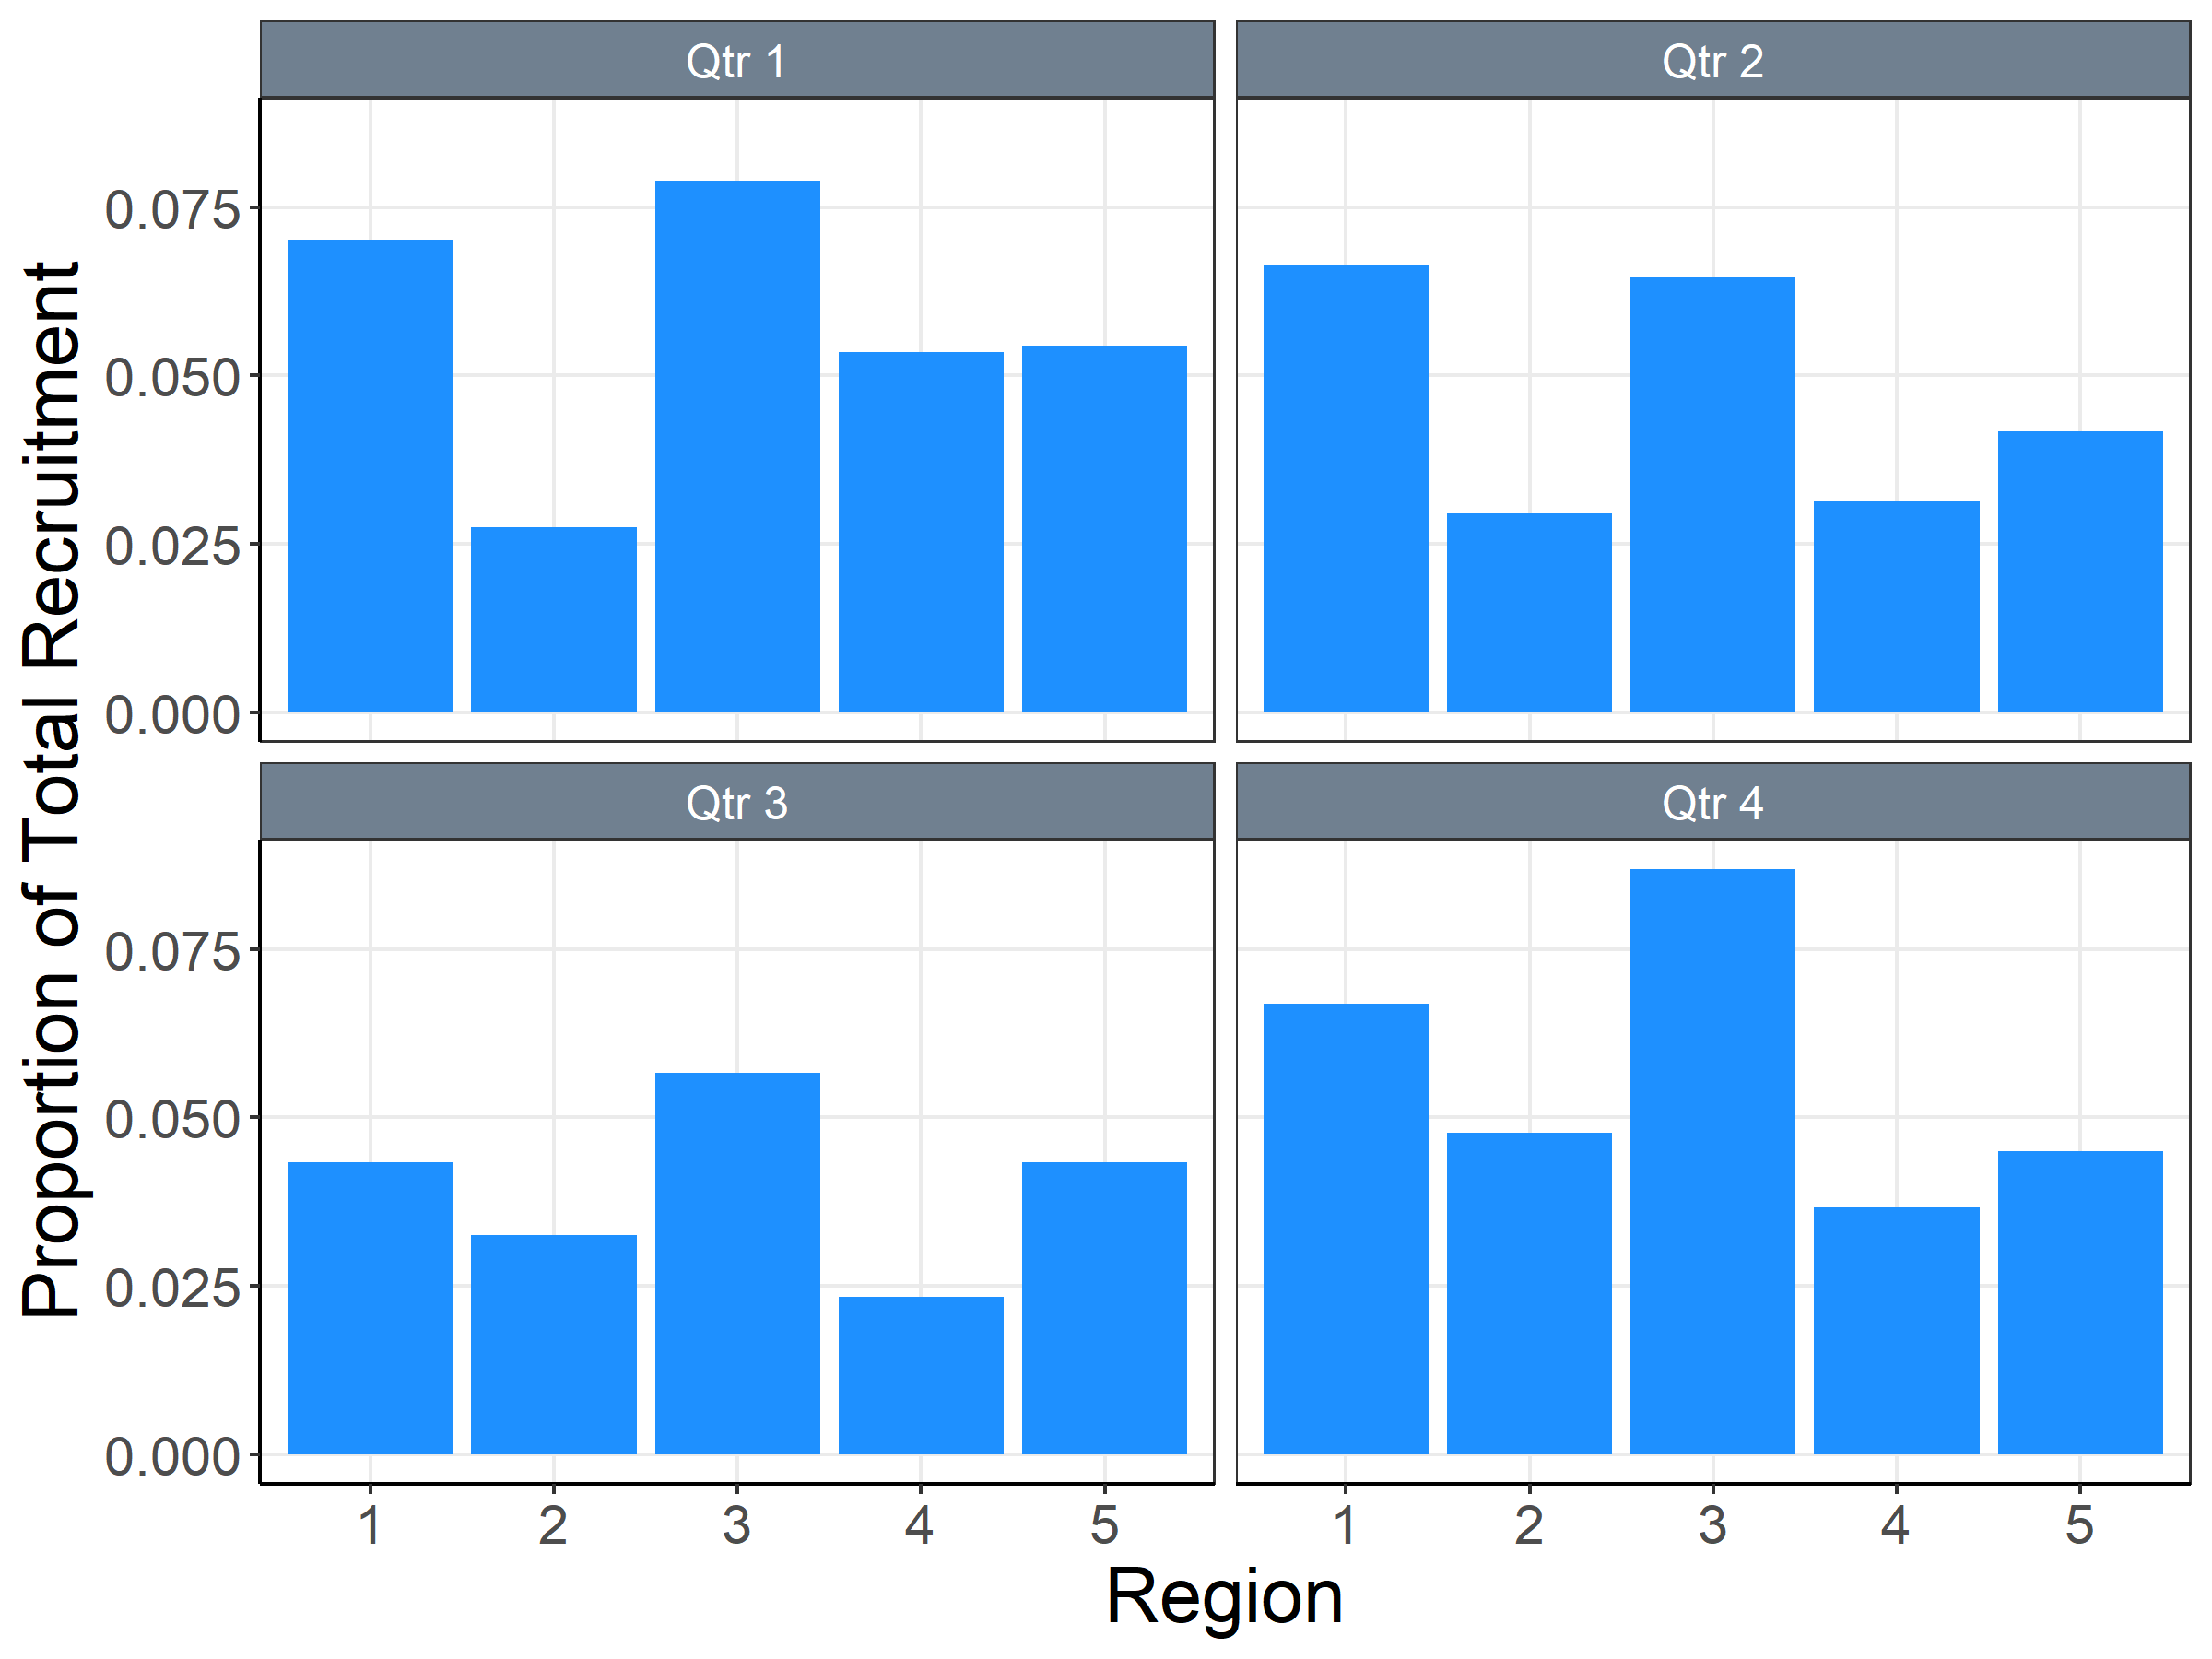
\includegraphics[width=1\linewidth,height=\textheight,keepaspectratio]{figures/recruitment_regions.png}

}

\caption{\label{fig-recruitment-regions}Estimated recruitment
distribution by region and quarter.}

\end{figure}%

\DIFdelbegin %DIFDELCMD < \begin{figure}[H]
%DIFDELCMD <

%DIFDELCMD < \centering{
%DIFDELCMD <

%DIFDELCMD < 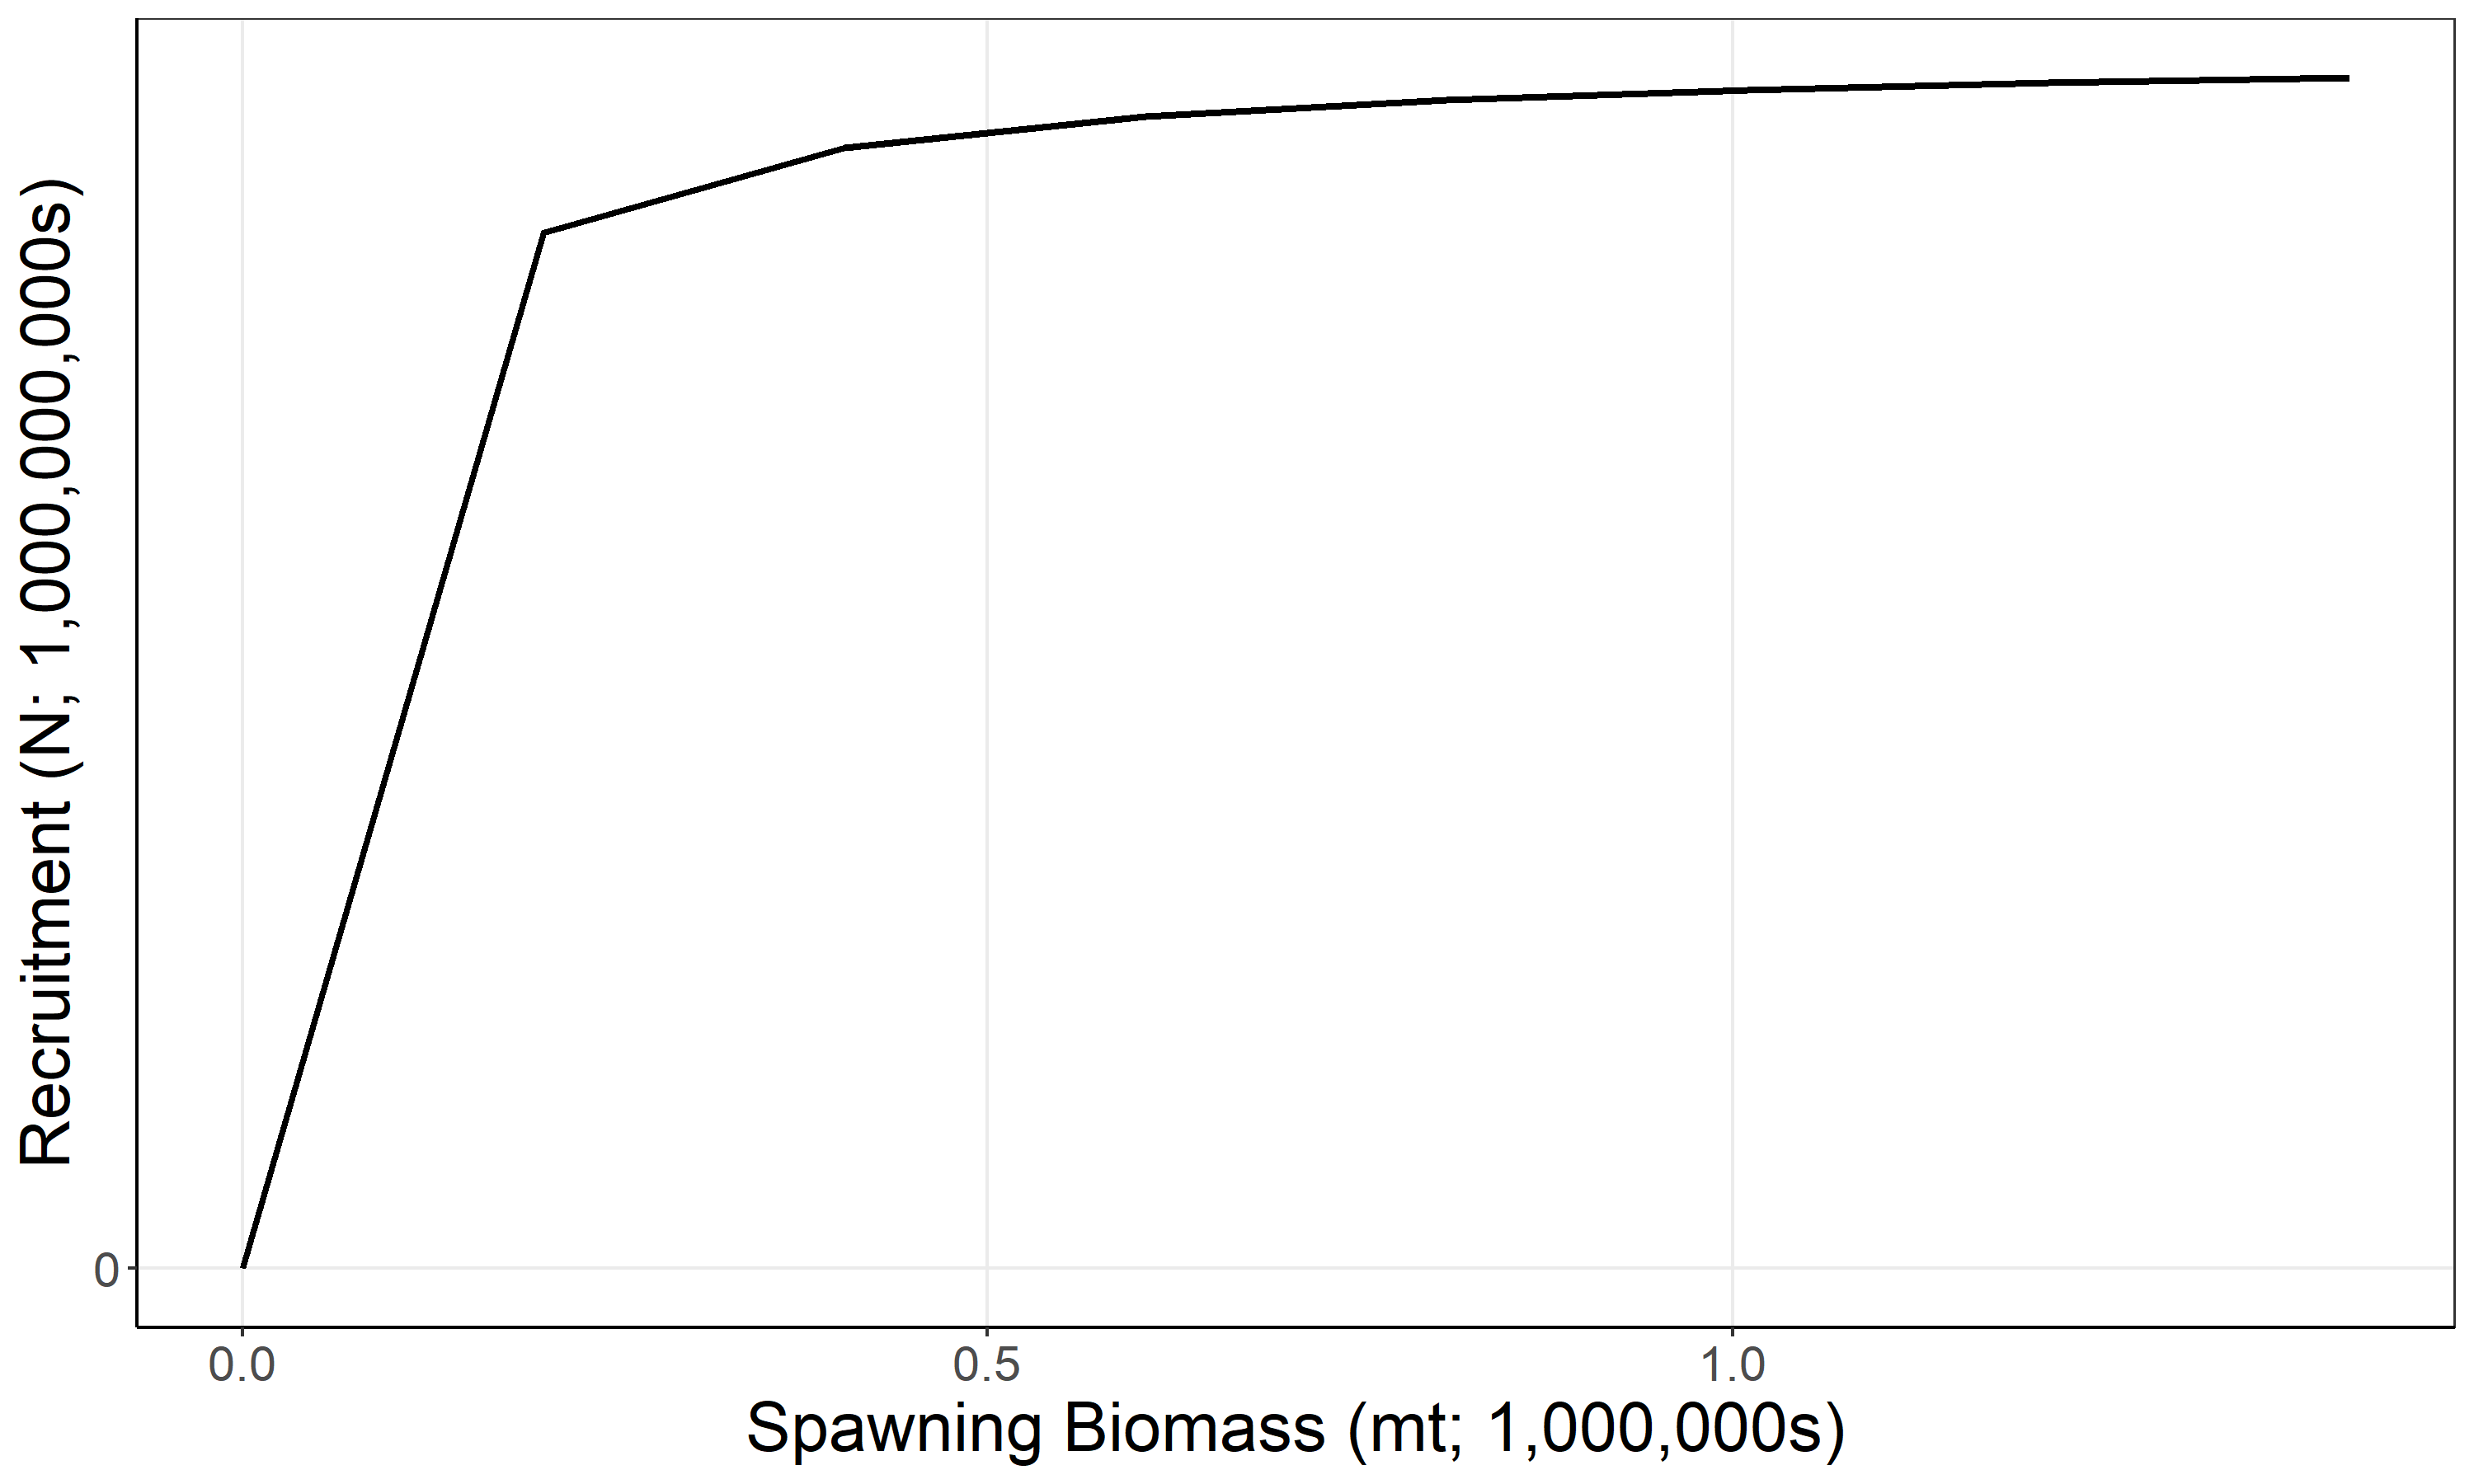
\includegraphics[width=1\linewidth,height=\textheight,keepaspectratio]{figures/stock_rr.png}
%DIFDELCMD <

%DIFDELCMD < }
%DIFDELCMD <

%DIFDELCMD < \caption{\label{fig-stock-rr}Estimated stock-recruitment relationship
%DIFDELCMD < between recruitment and spawning potential based on annual estimates of
%DIFDELCMD < recruitment for the 2023 diagnostic model. The colour of the circles
%DIFDELCMD < transitions from purple (early in the time series) to yellow (more
%DIFDELCMD < recent) through time. Points shown prior to 1968 are not used in the fit
%DIFDELCMD < to the stock recruitment relationship.}
%DIFDELCMD <

%DIFDELCMD < \end{figure}%%%
\DIFdelend \DIFaddbegin \begin{figure}[H]

\centering{

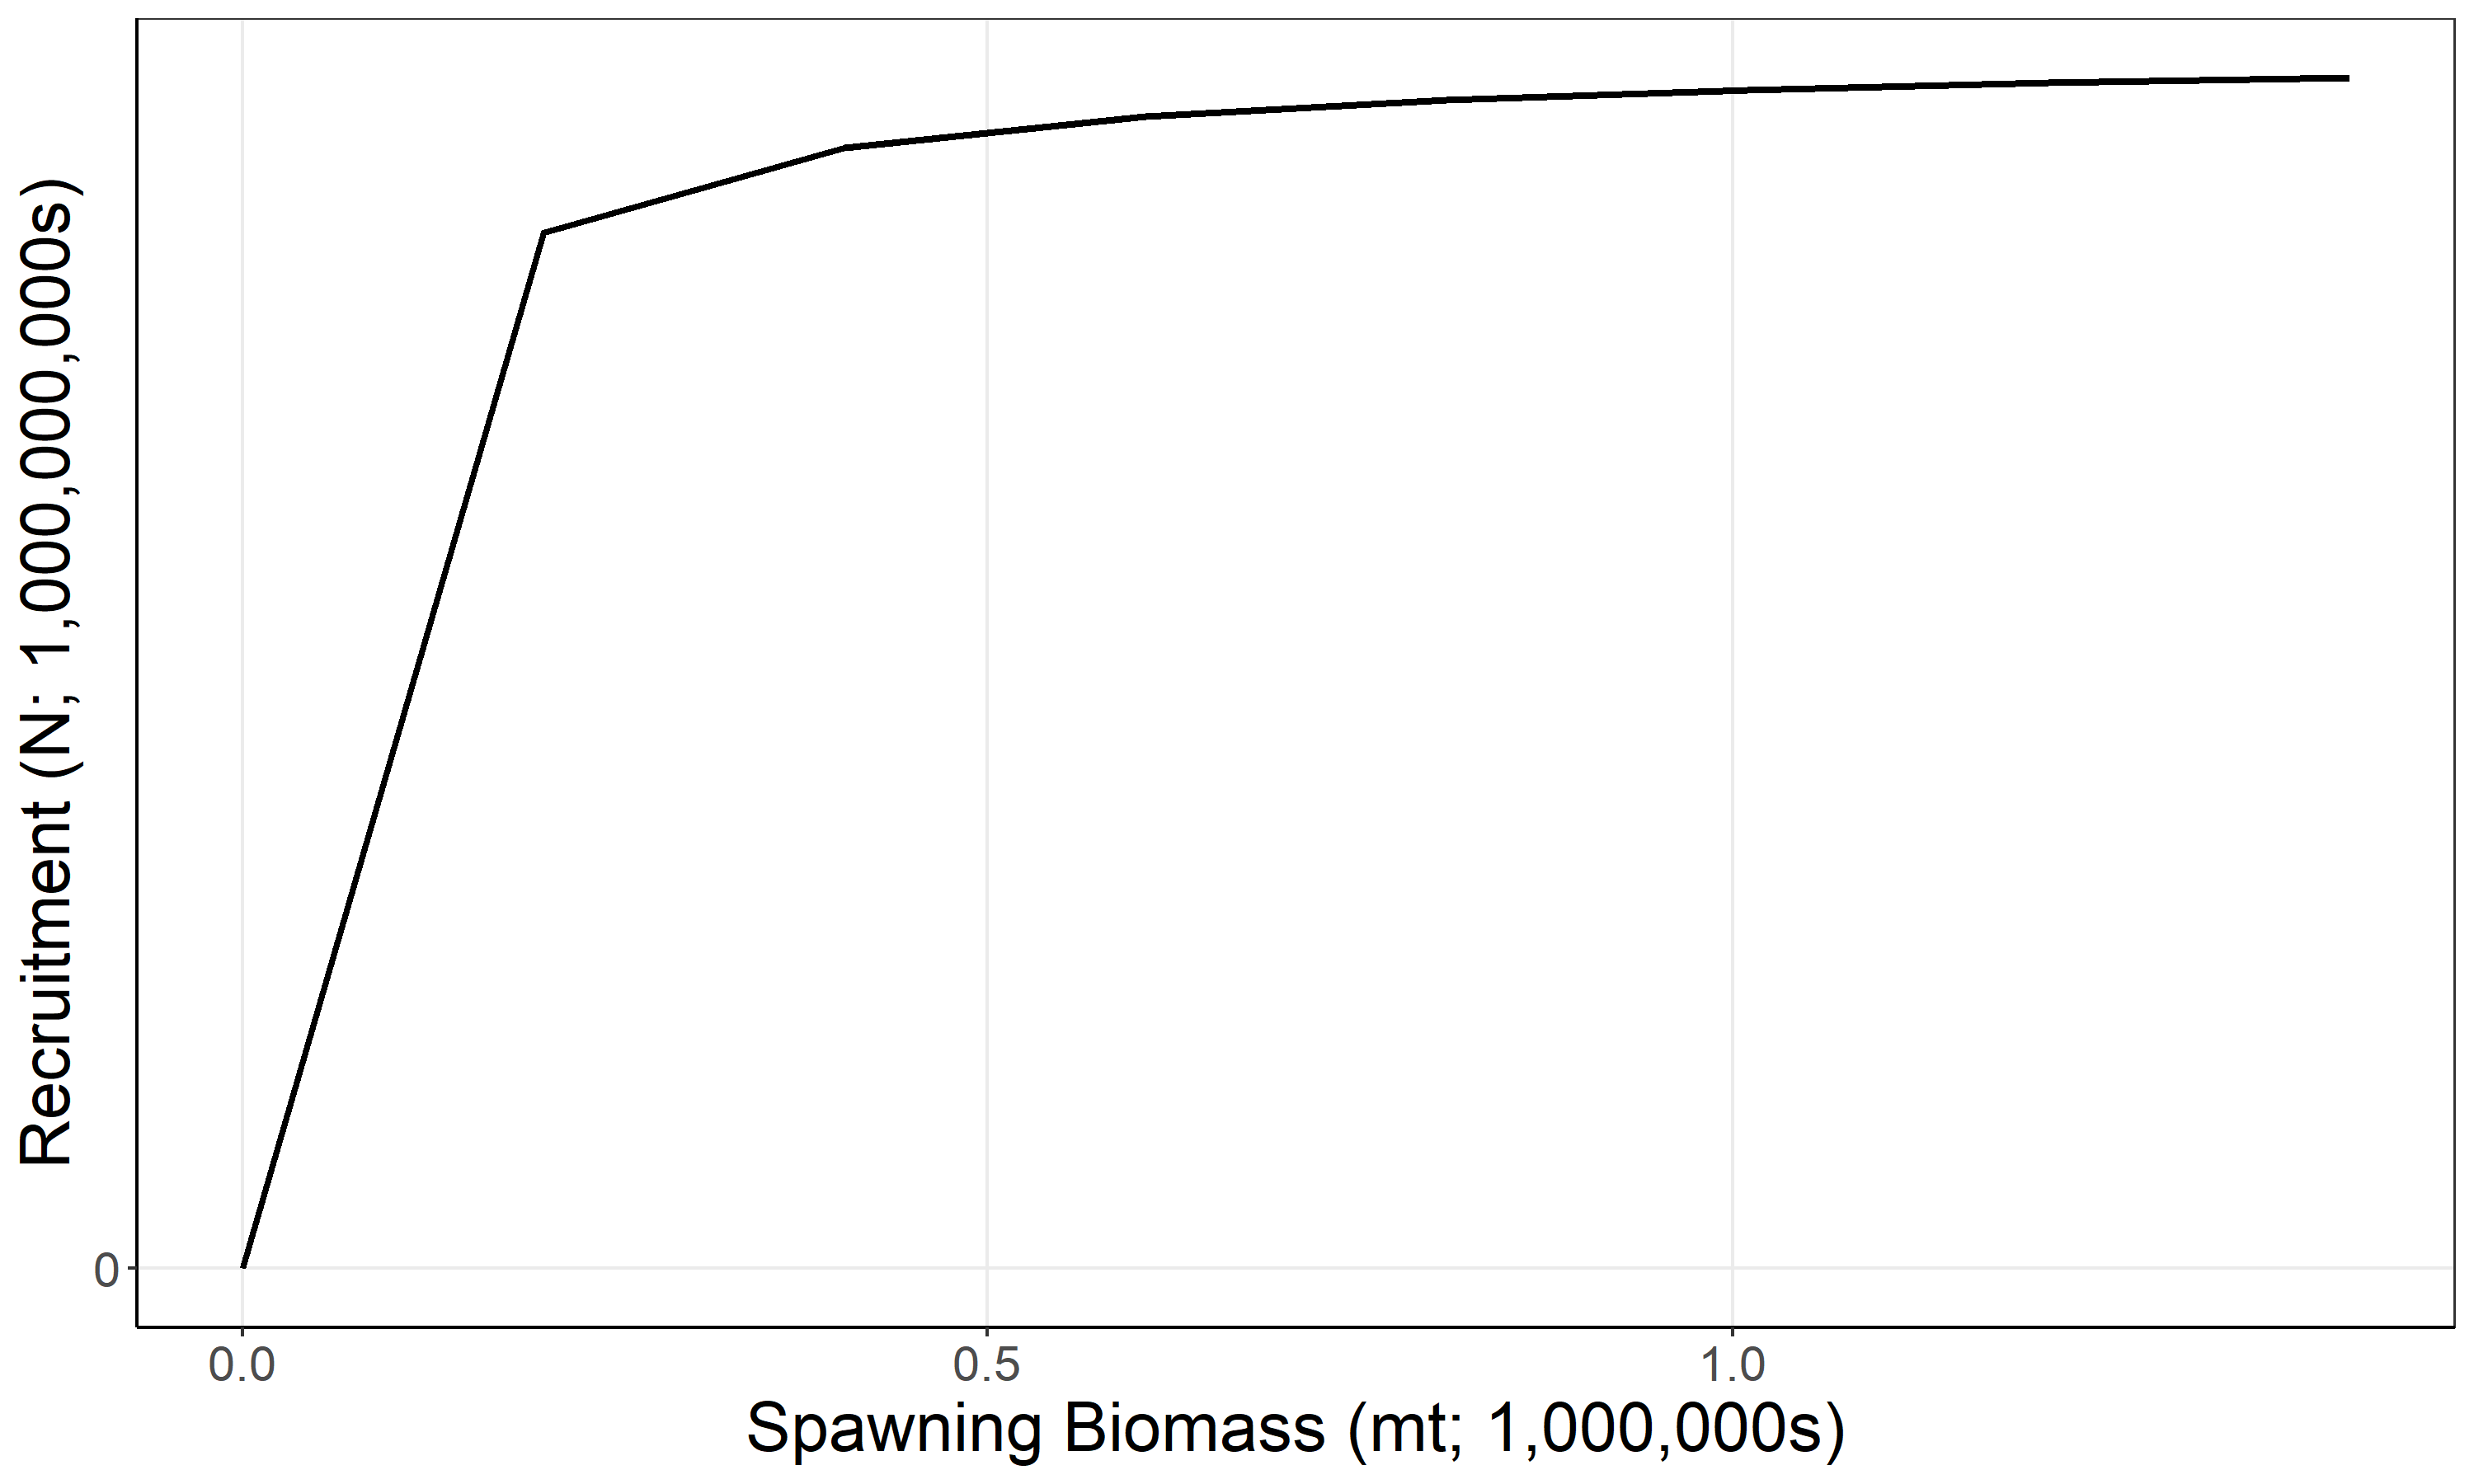
\includegraphics[width=1\linewidth,height=\textheight,keepaspectratio]{figures/stock_rr.png}

}

\caption{\label{fig-stock-rr}Estimated stock--recruitment relationship
between recruitment and spawning potential based on annual estimates
from the 2026 diagnostic model. Circle colour progresses from purple for
early years to yellow for recent years. Points before 1968 are not used
to fit the relationship.}

\end{figure}\DIFaddend %

\begin{figure}[H]

\centering{

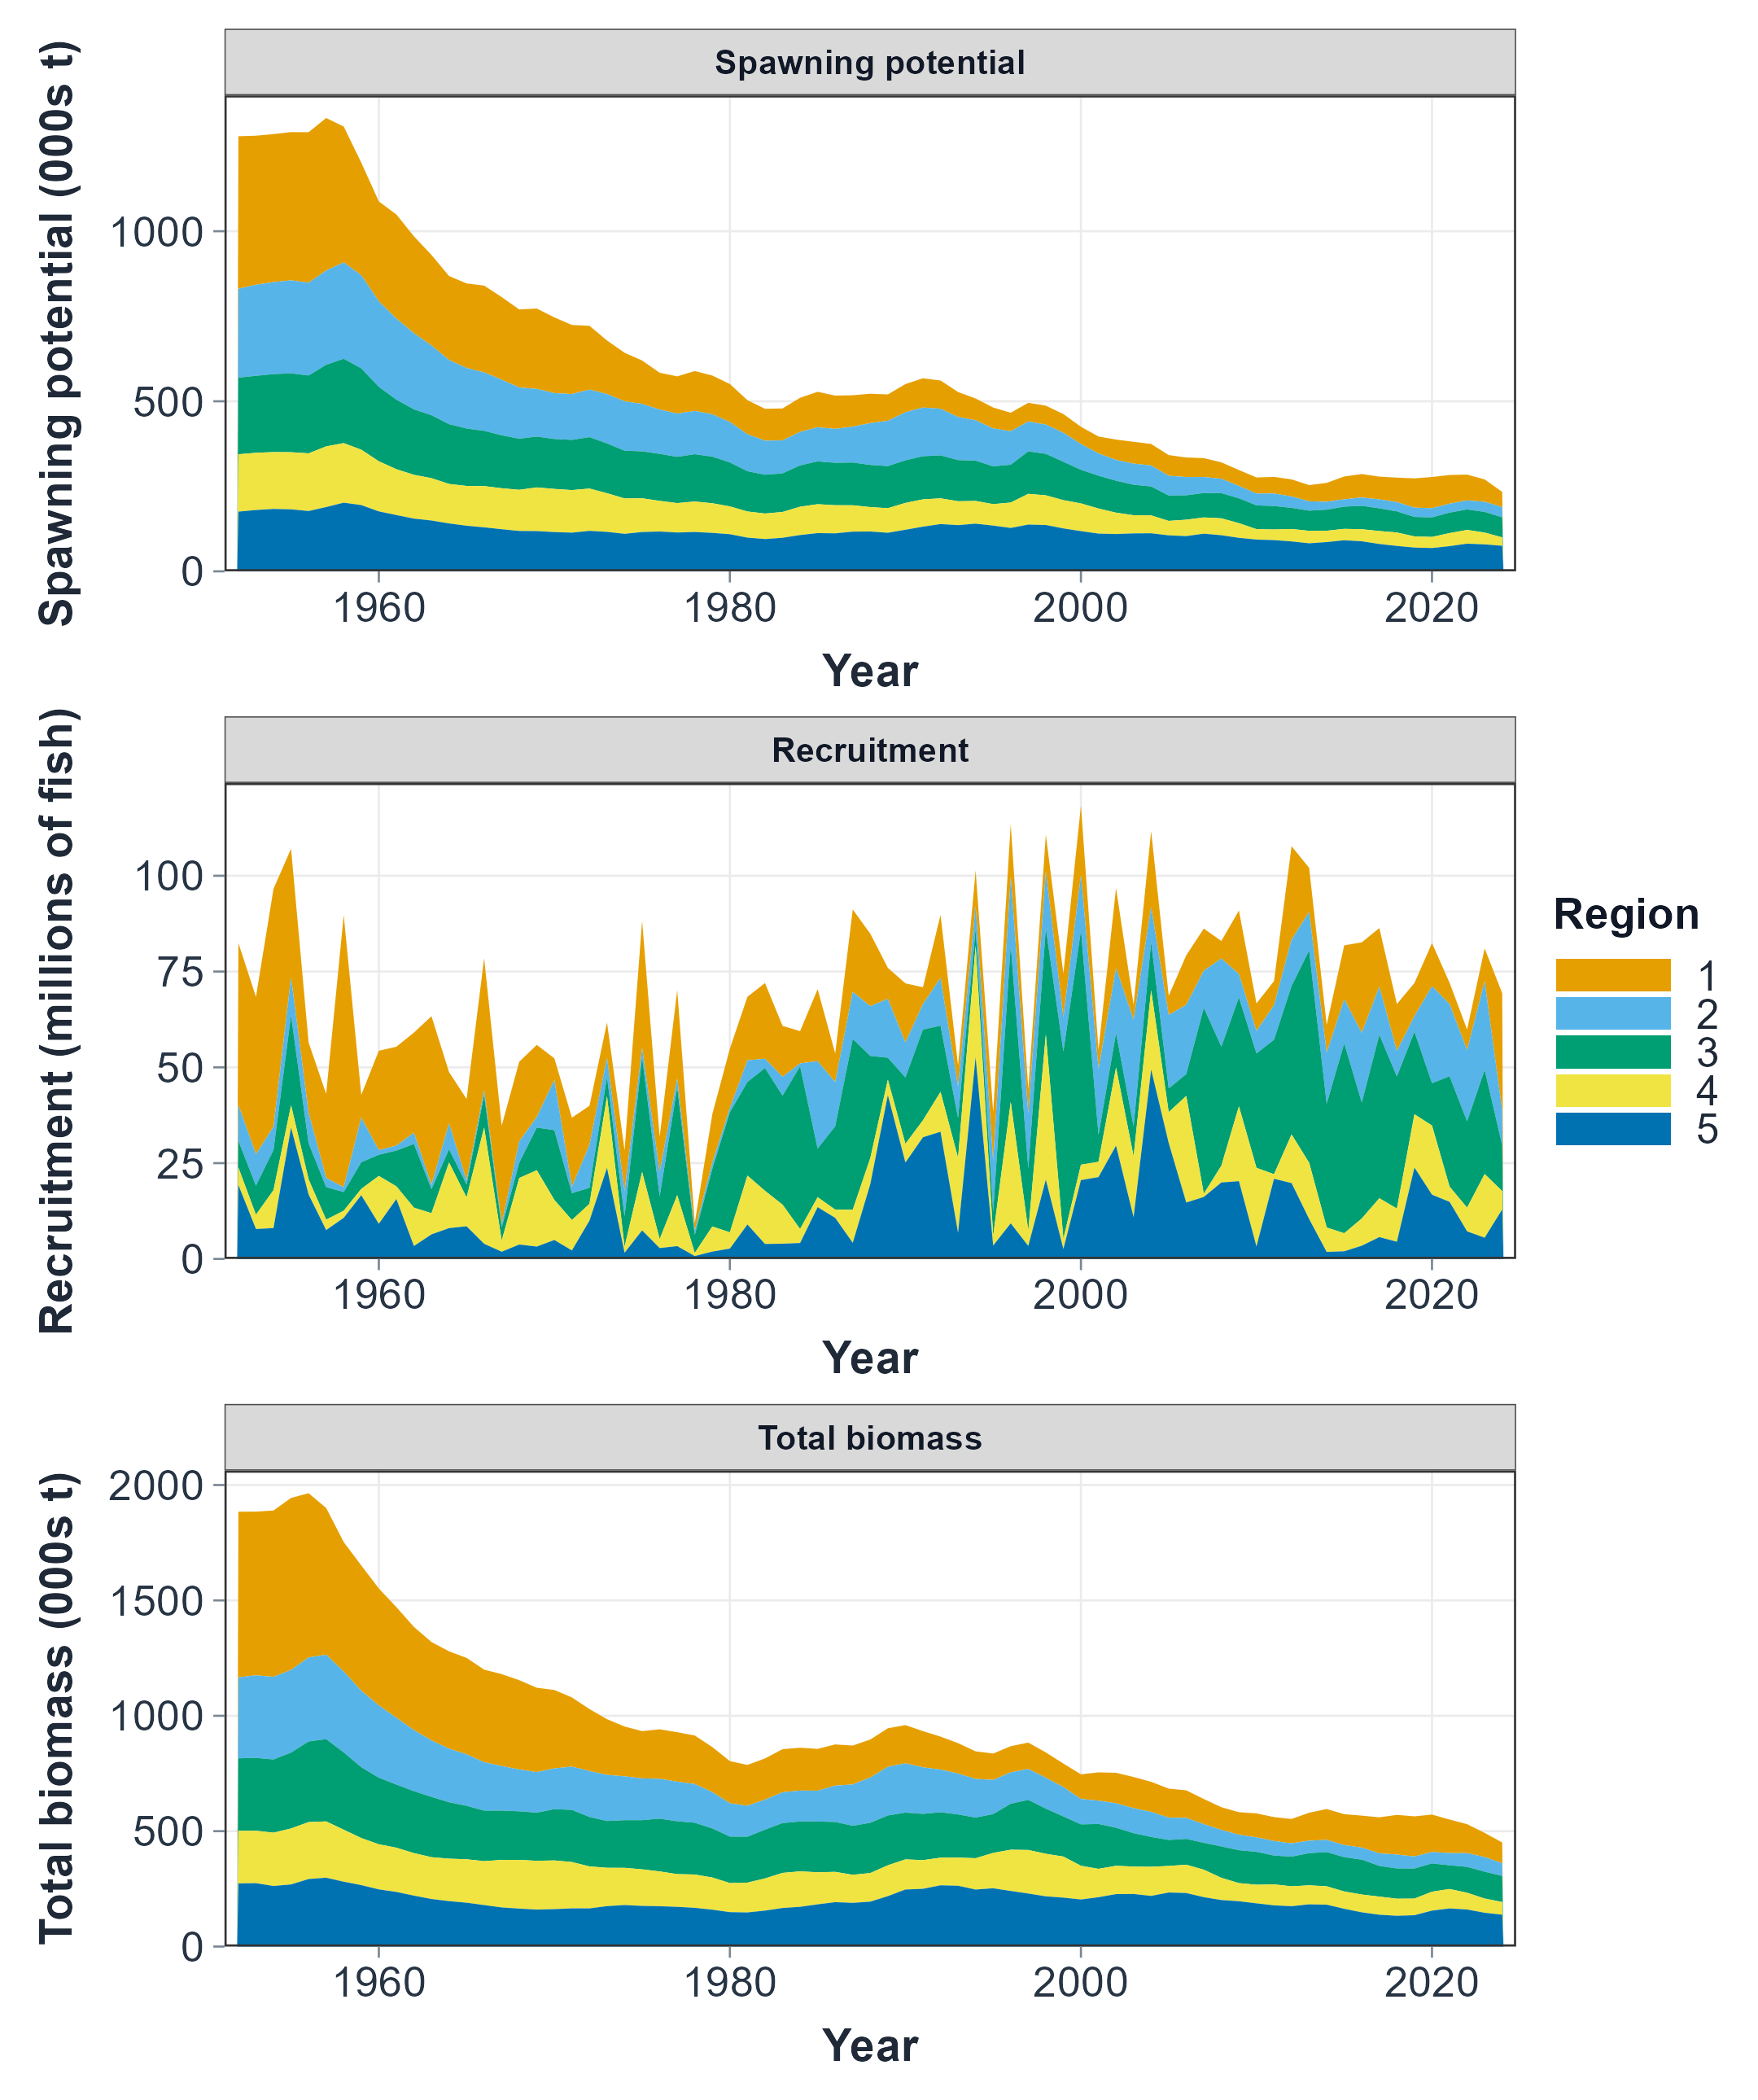
\includegraphics[width=1\linewidth,height=\textheight,keepaspectratio]{figures/timeseries_model_regions_stack.png}

}

\caption{\label{fig-timeseries-model-regions-stack}Time series of
estimated annual spawning potential, recruitment and total biomass by
model region for the diagnostic model, showing the relative proportions
among regions. Note the data represent the averages of the quarterly
model time steps for each year for spawning potential and total biomass
and the sum of the quarterly recruitment estimates for annual
recruitment.}

\end{figure}%

\DIFdelbegin %DIFDELCMD < \begin{figure}[H]
%DIFDELCMD <

%DIFDELCMD < \centering{
%DIFDELCMD <

%DIFDELCMD < 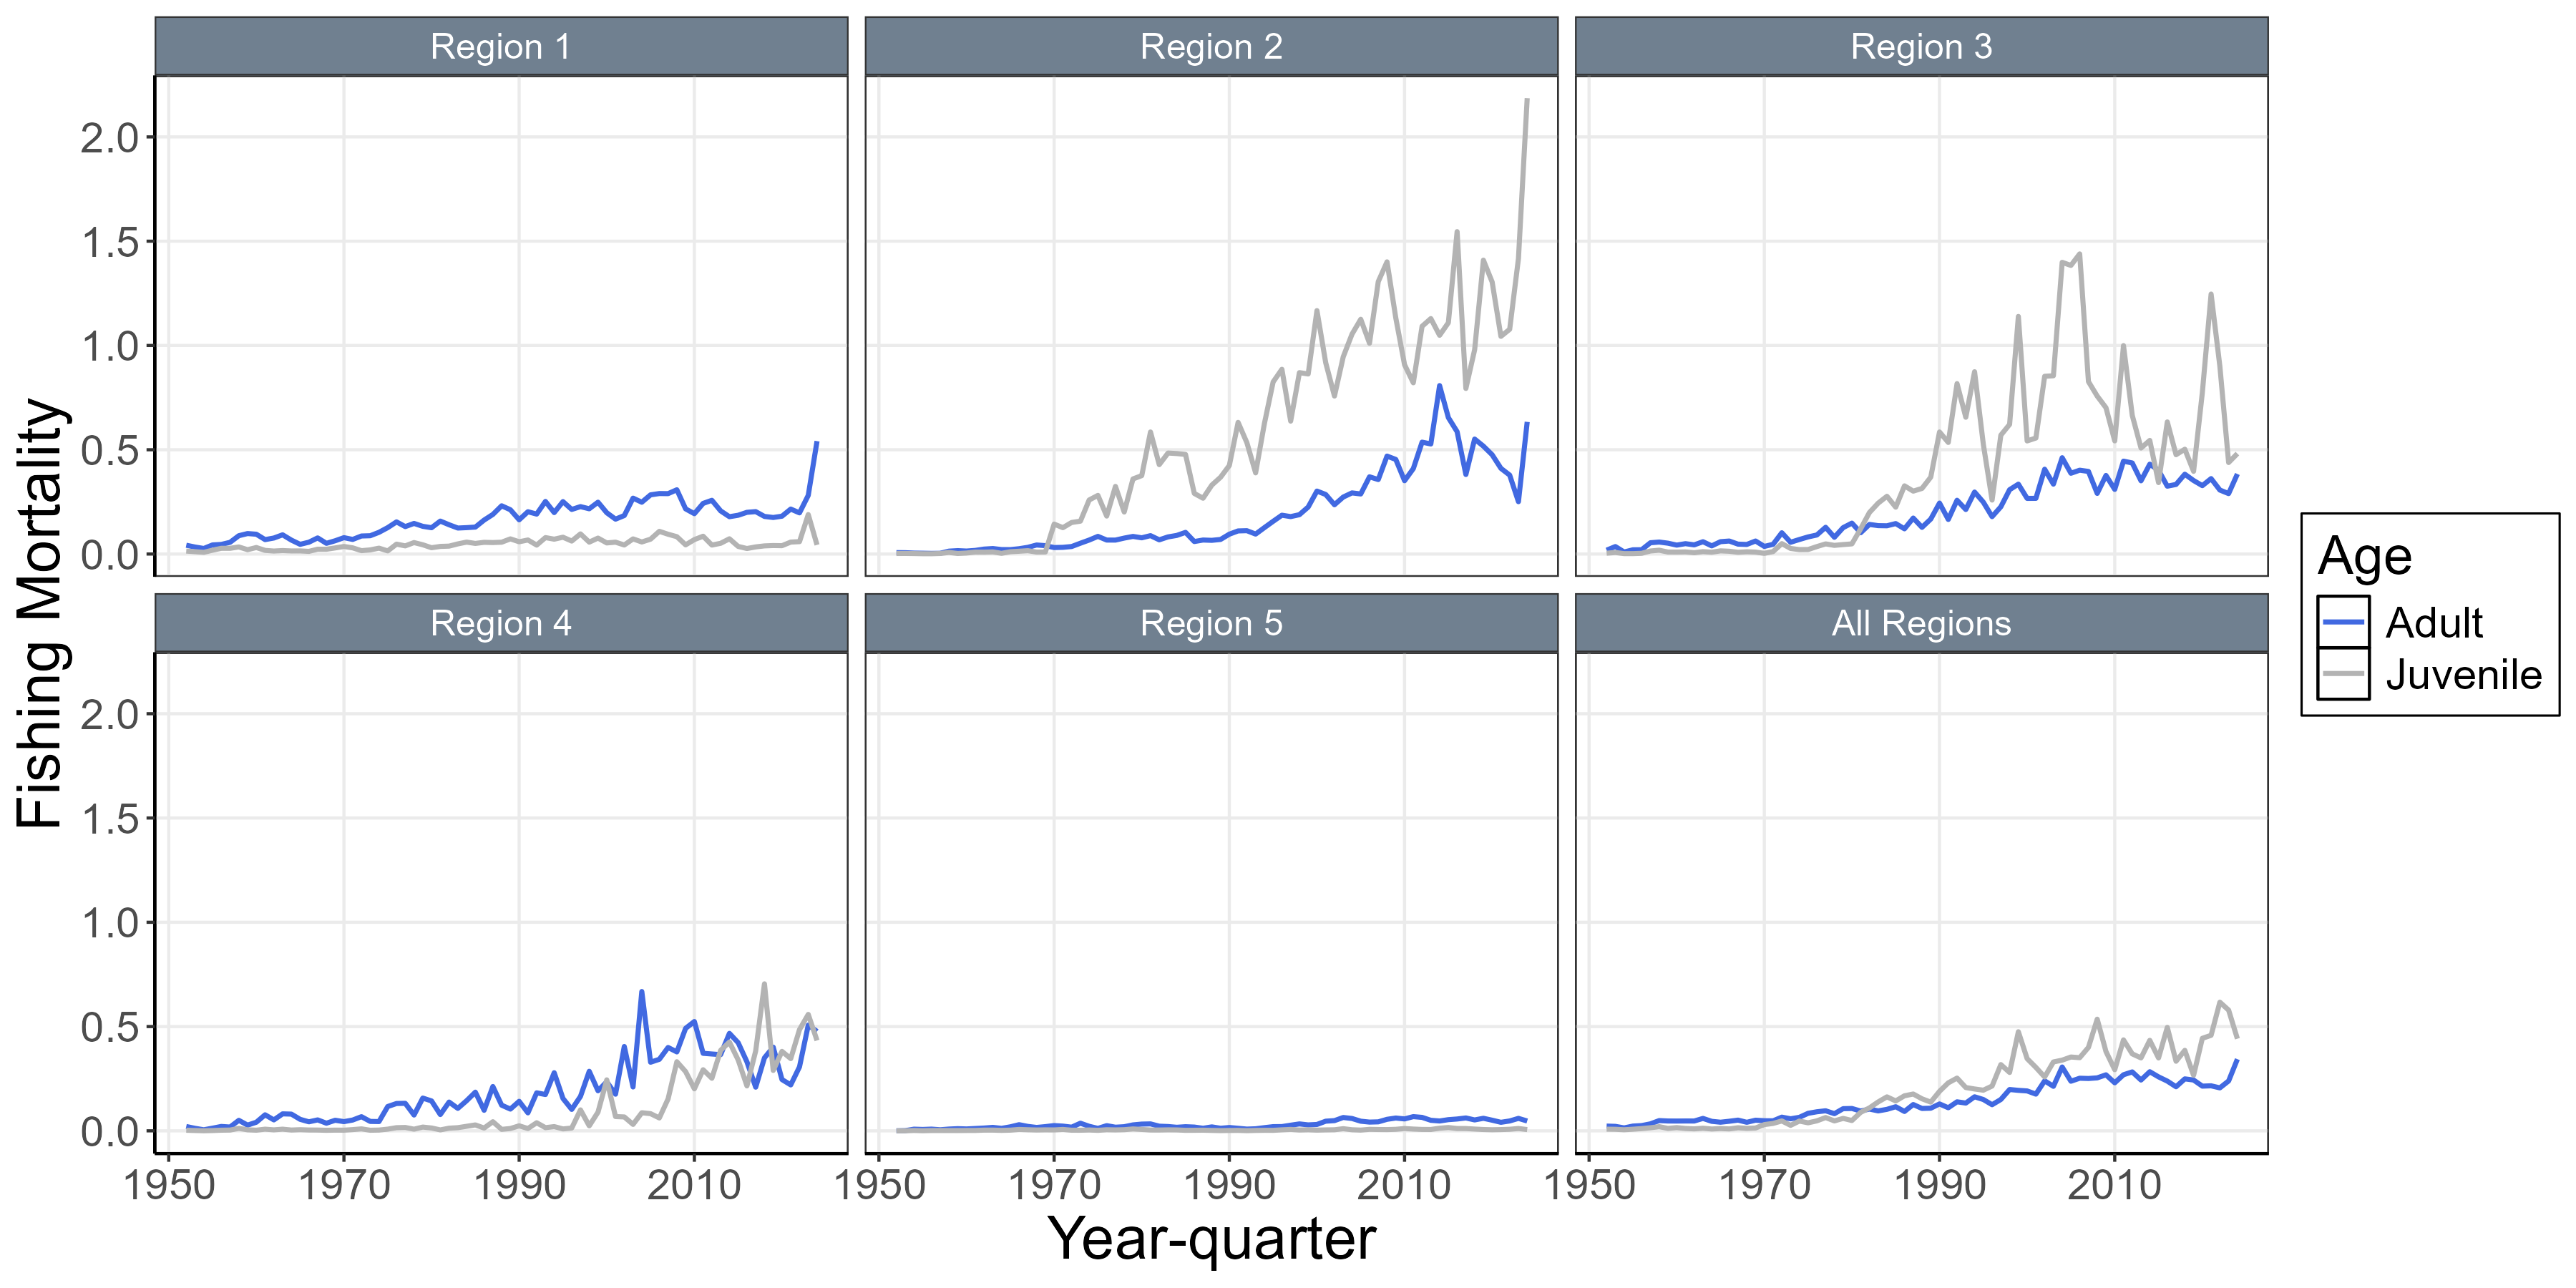
\includegraphics[width=1\linewidth,height=\textheight,keepaspectratio]{figures/F_adult_juv_regions.png}
%DIFDELCMD <

%DIFDELCMD < }
%DIFDELCMD <

%DIFDELCMD < \caption{\label{fig-F-adult-juv-regions}Estimated annual average adult
%DIFDELCMD < (solid line) and juvenile (dashed line) fishing mortality for the 2023
%DIFDELCMD < diagnostic model by model region and across all regions.}
%DIFDELCMD <

%DIFDELCMD < \end{figure}%%%
\DIFdelend \DIFaddbegin \begin{figure}[H]

\centering{

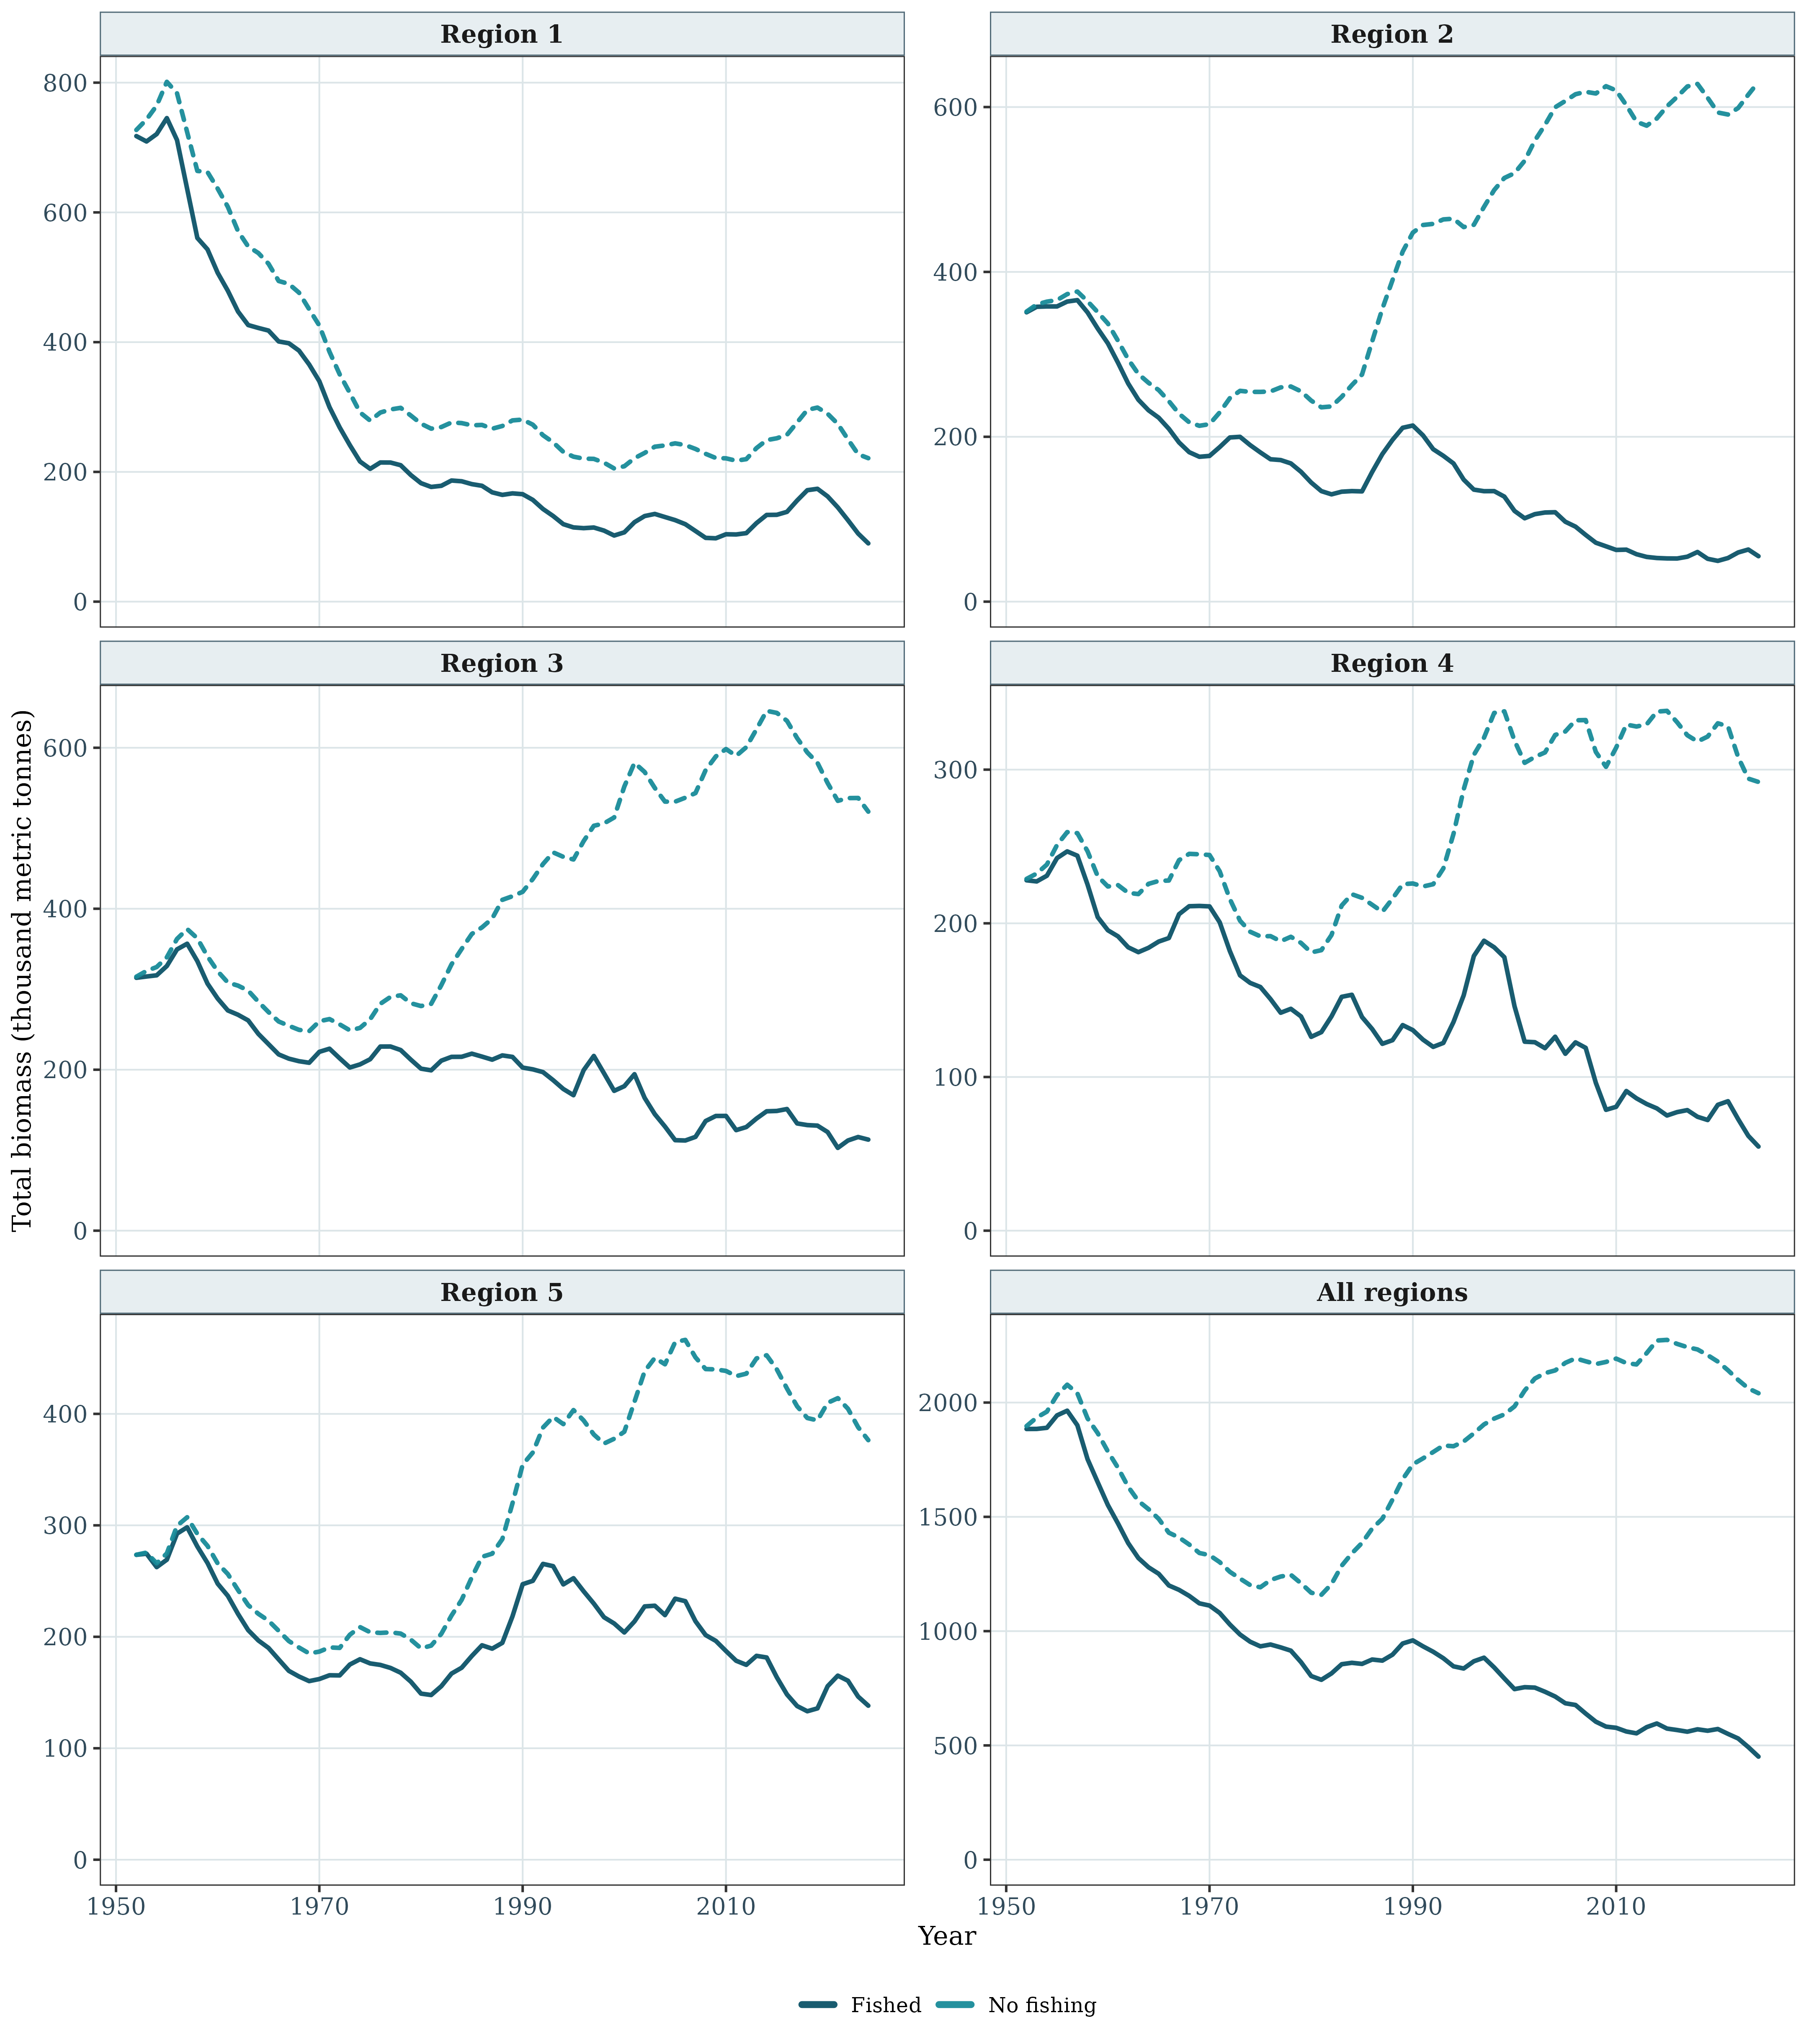
\includegraphics[width=1\linewidth,height=\textheight,keepaspectratio]{figures_new/total-biomass-with-without-fishing-2col.png}

}

\caption{\label{fig-total-biomass-with-without-fishing}Estimated annual
total biomass by model region and over all regions under the fitted
fishing history (solid dark line) and the dynamic no-fishing
counterfactual (dashed teal line). Annual values average the four
quarterly estimates. The two-column layout provides additional panel
height; panel y axes are free and begin at zero.}

\end{figure}\DIFaddend %

\DIFdelbegin %DIFDELCMD < \begin{figure}[H]
%DIFDELCMD <

%DIFDELCMD < \centering{
%DIFDELCMD <

%DIFDELCMD < 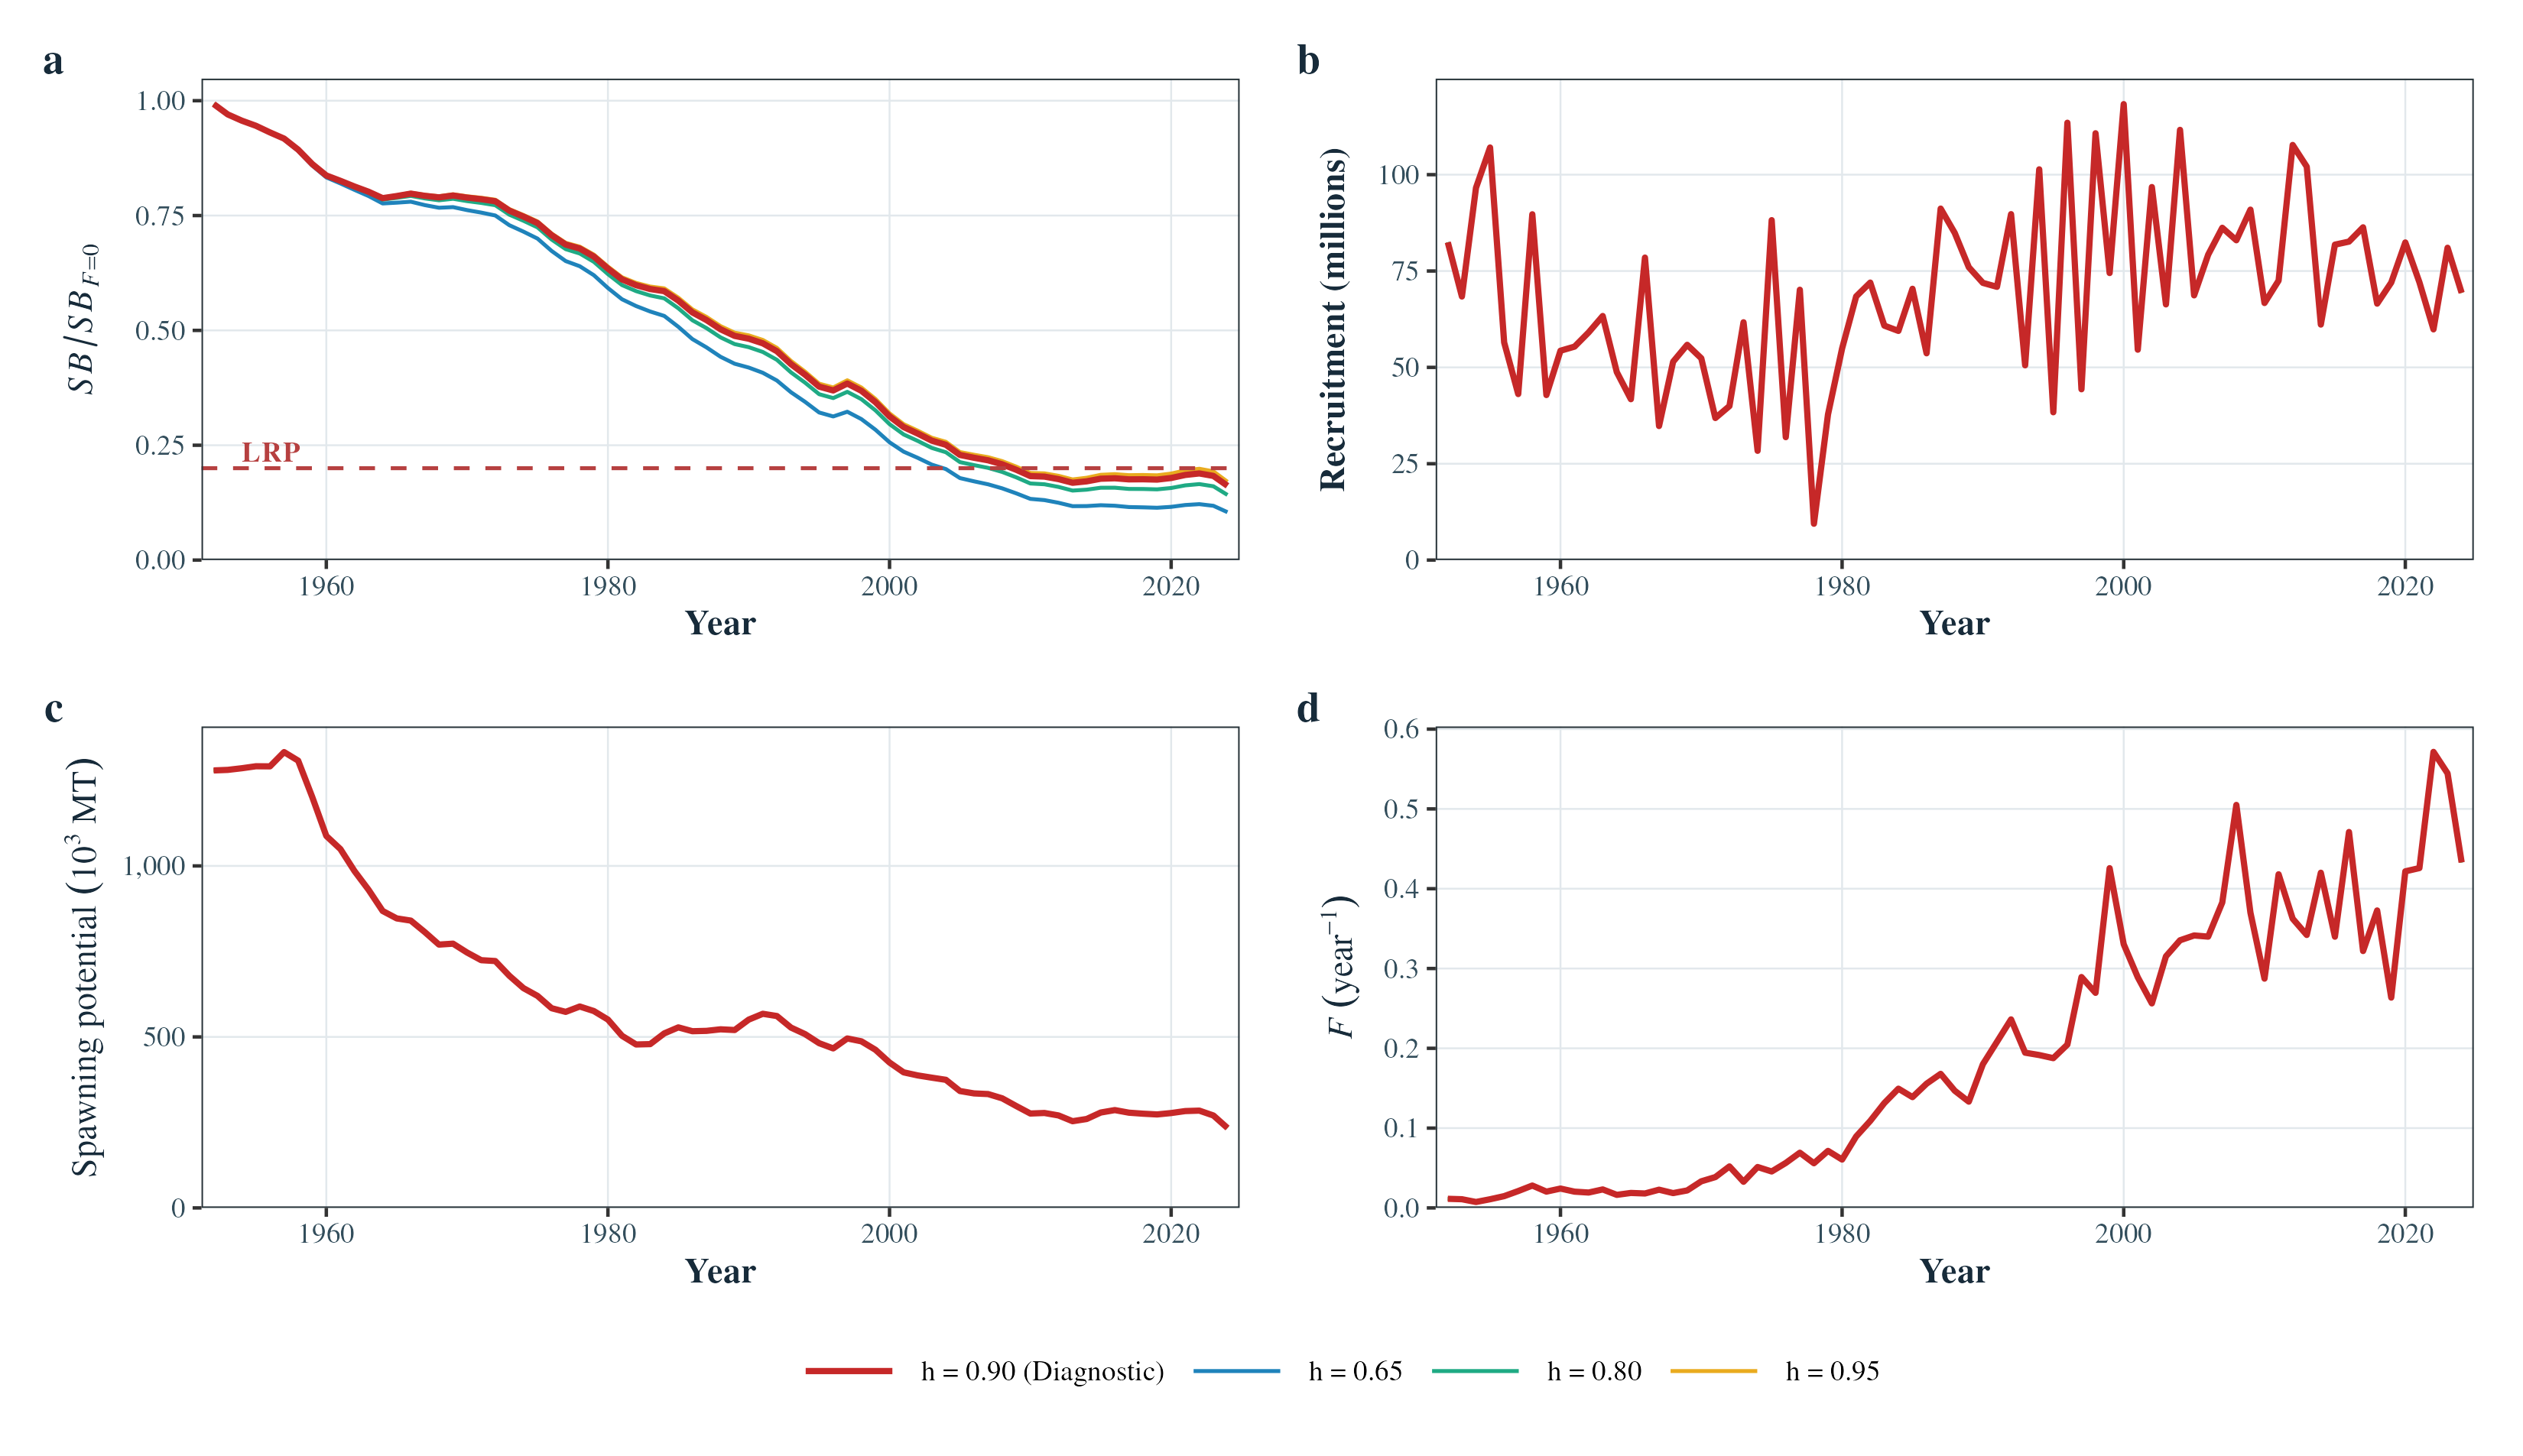
\includegraphics[width=1\linewidth,height=\textheight,keepaspectratio]{figures/sensitivity_steepness.png}
%DIFDELCMD <

%DIFDELCMD < }
%DIFDELCMD <

%DIFDELCMD < \caption{\label{fig-sensitivity-steepness}Estimated dynamic spawning
%DIFDELCMD < depletion (Top left) and spawning potential (Bottom left), recruitment
%DIFDELCMD < (Top right) and fishing mortality (Bottom right) for the one-off
%DIFDELCMD < sensitivities from the 2026 diagnostic model for steepness of the stock
%DIFDELCMD < recruitment relationship.}
%DIFDELCMD <

%DIFDELCMD < \end{figure}%%%
\DIFdelend \DIFaddbegin \begin{figure}[H]

\centering{

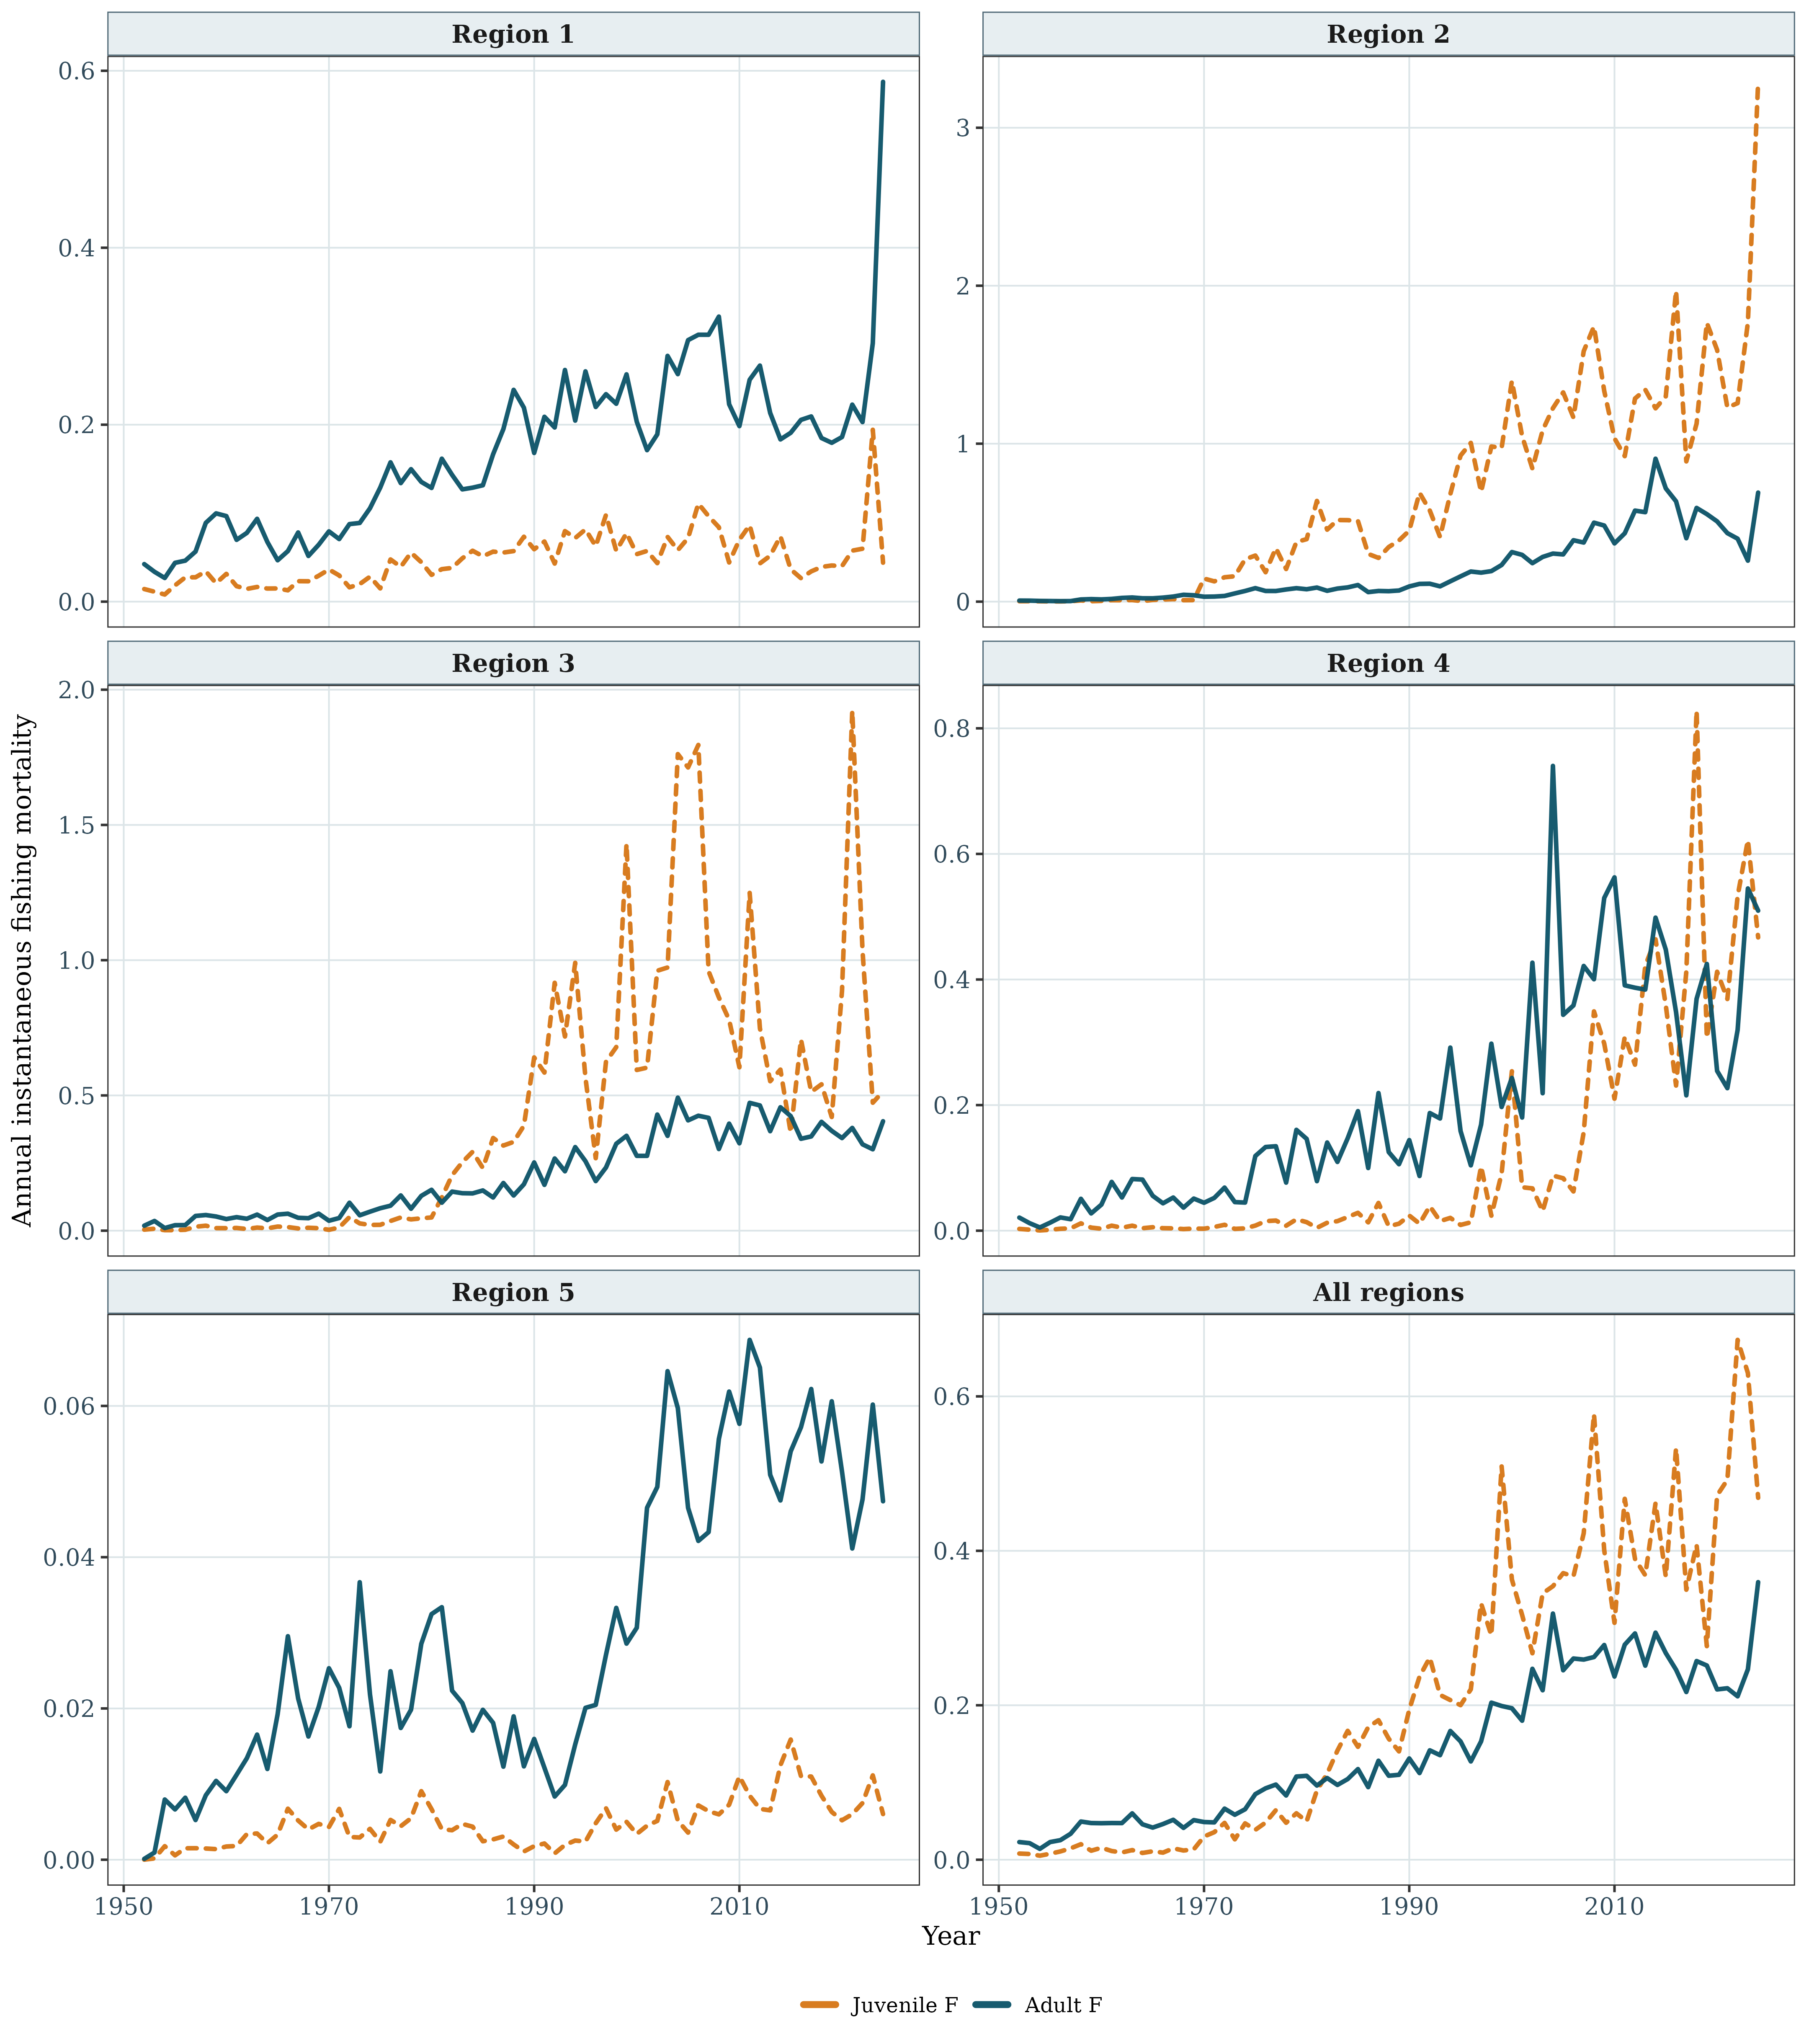
\includegraphics[width=1\linewidth,height=\textheight,keepaspectratio]{figures_new/f-juvenile-adult-by-area-2col.png}

}

\caption{\label{fig-juv-adult-F}Annual juvenile (orange dashed) and
adult (dark solid) instantaneous fishing mortality by model region and
the pooled All regions series (last). The two-column layout provides
additional panel height; panel y axes are free and begin at zero.}

\end{figure}\DIFaddend %

\DIFdelbegin %DIFDELCMD < \begin{figure}[H]
%DIFDELCMD <

%DIFDELCMD < \centering{
%DIFDELCMD <

%DIFDELCMD < 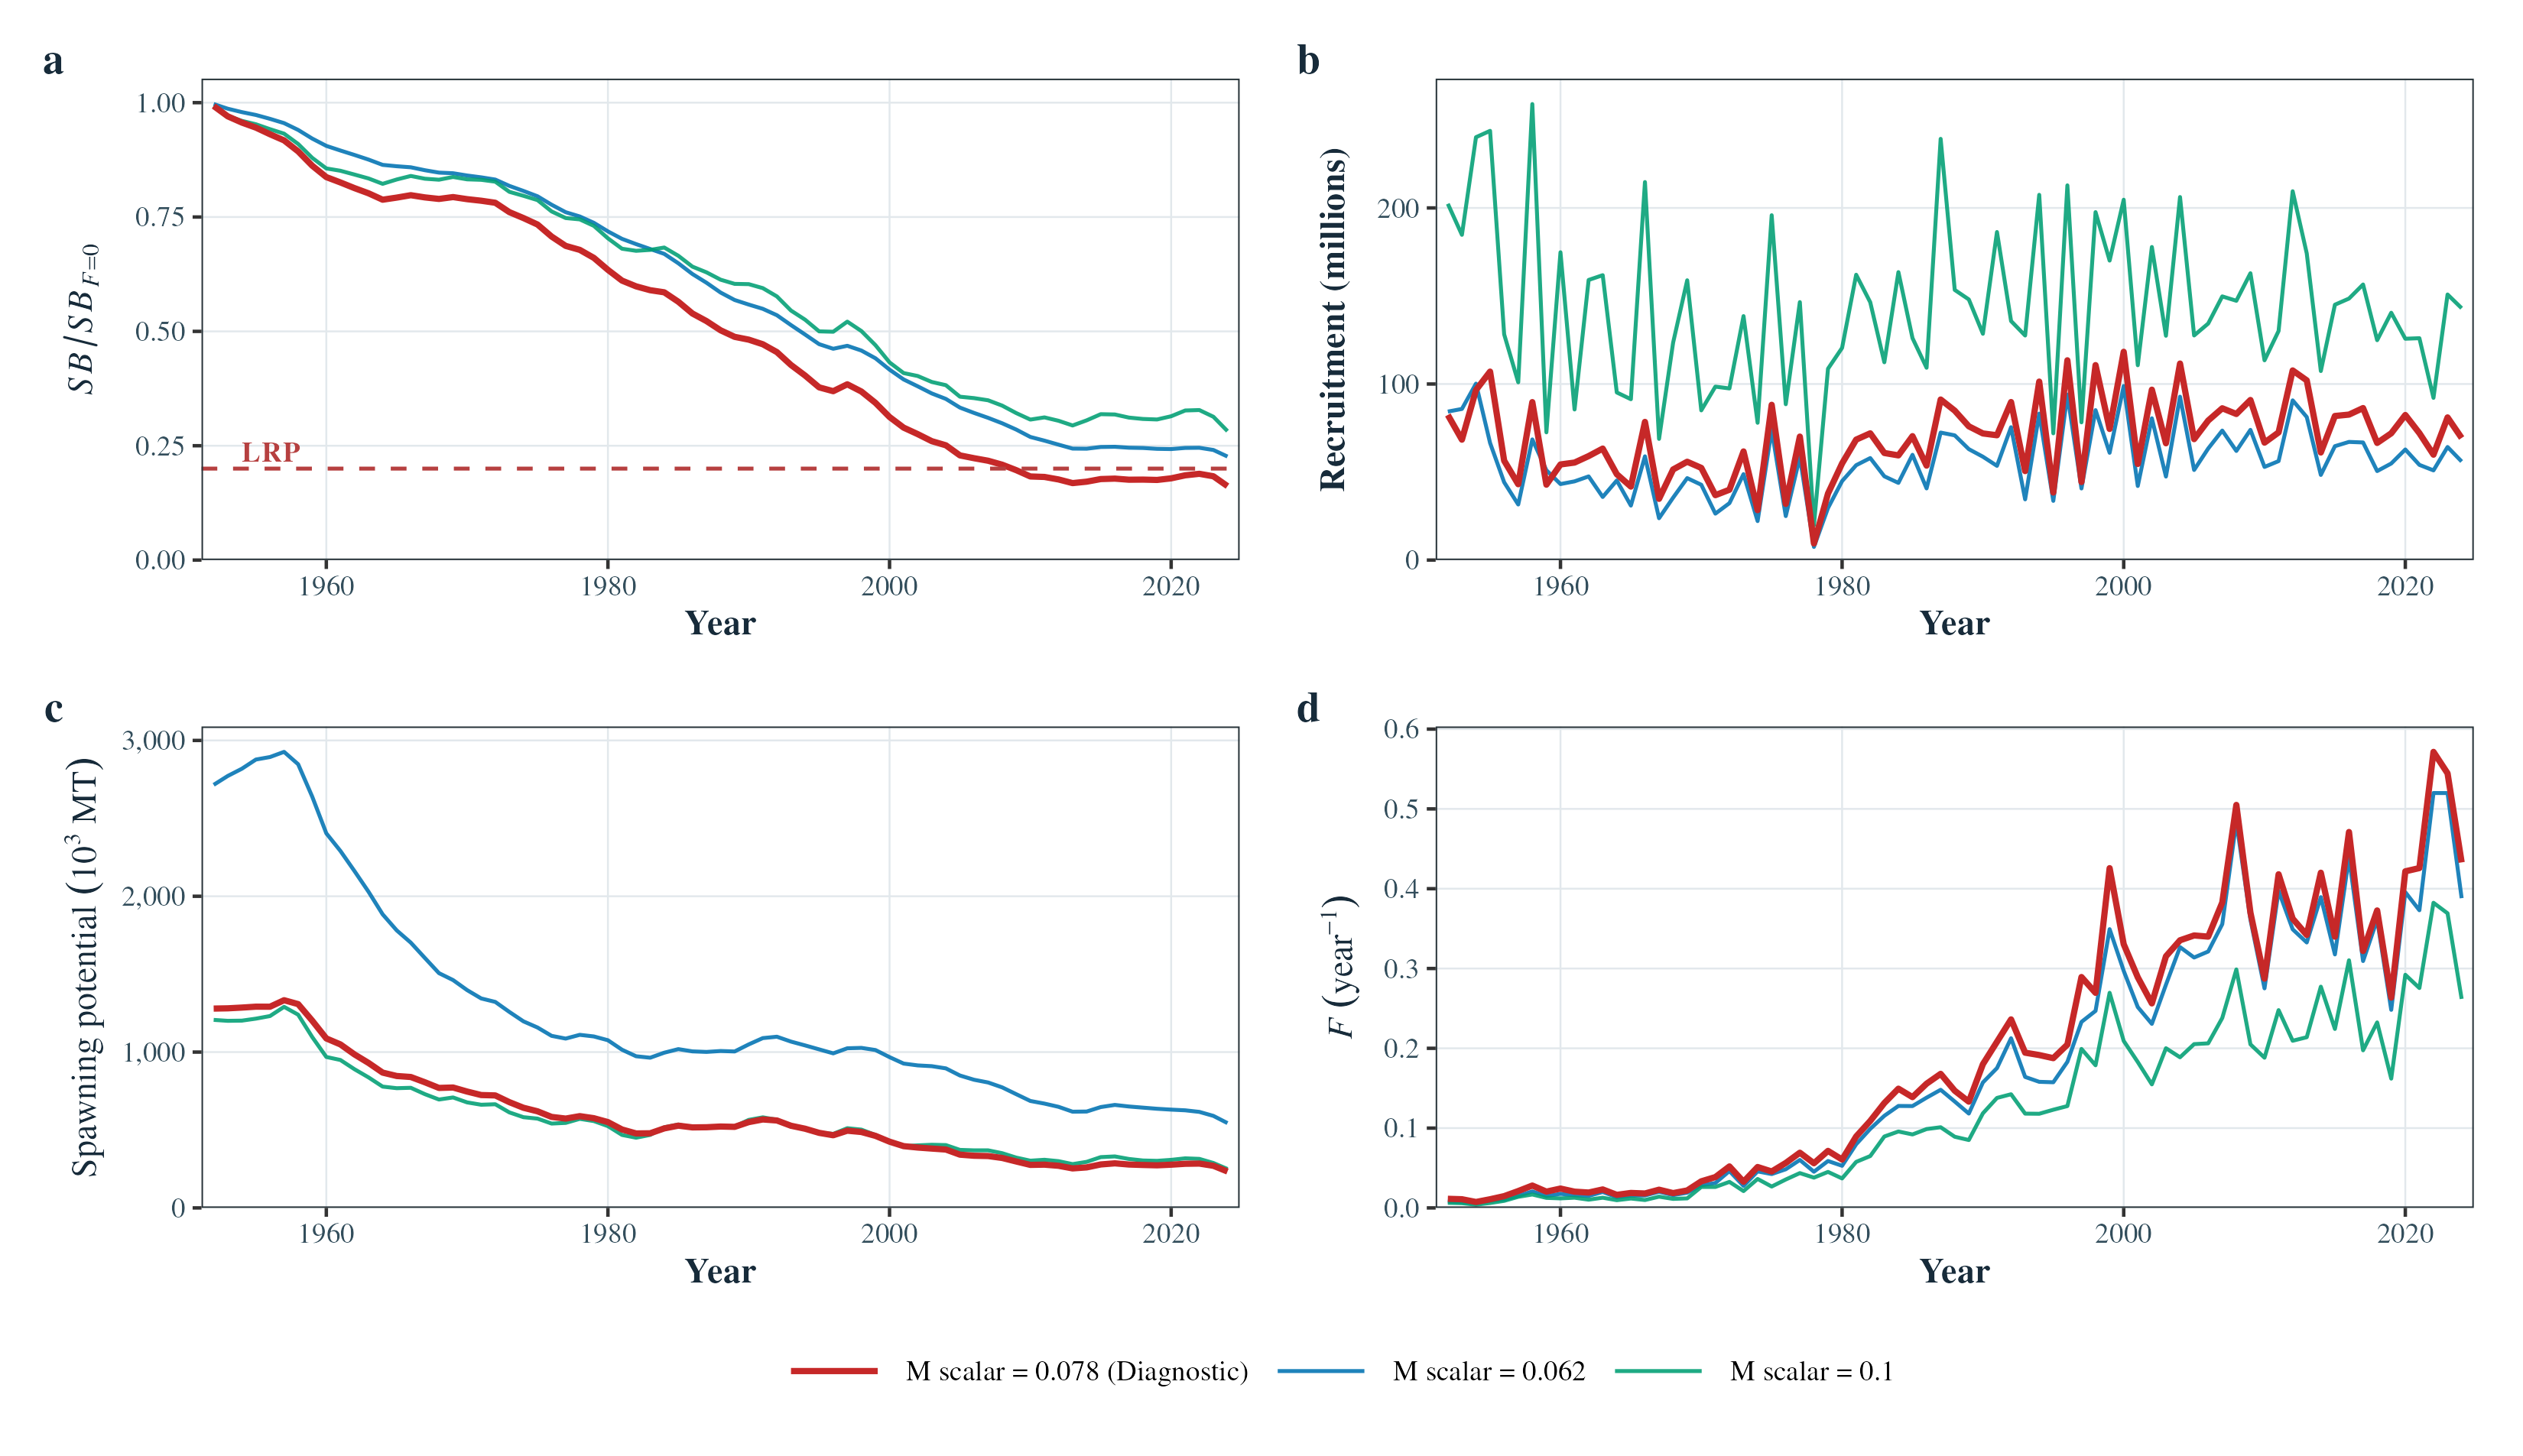
\includegraphics[width=1\linewidth,height=\textheight,keepaspectratio]{figures/sensitivity_natural_mortality.png}
%DIFDELCMD <

%DIFDELCMD < }
%DIFDELCMD <

%DIFDELCMD < \caption{\label{fig-sensitivity-natural-mortality}Estimated dynamic
%DIFDELCMD < spawning depletion (Top left) and spawning potential (Bottom left),
%DIFDELCMD < recruitment (Top right) and fishing mortality (Bottom right) for the
%DIFDELCMD < one-off sensitivities from the 2026 diagnostic model for natural
%DIFDELCMD < mortality scale (M at age 40 quarters).}
%DIFDELCMD <

%DIFDELCMD < \end{figure}%%%
\DIFdelend \DIFaddbegin \begin{figure}[H]

\centering{

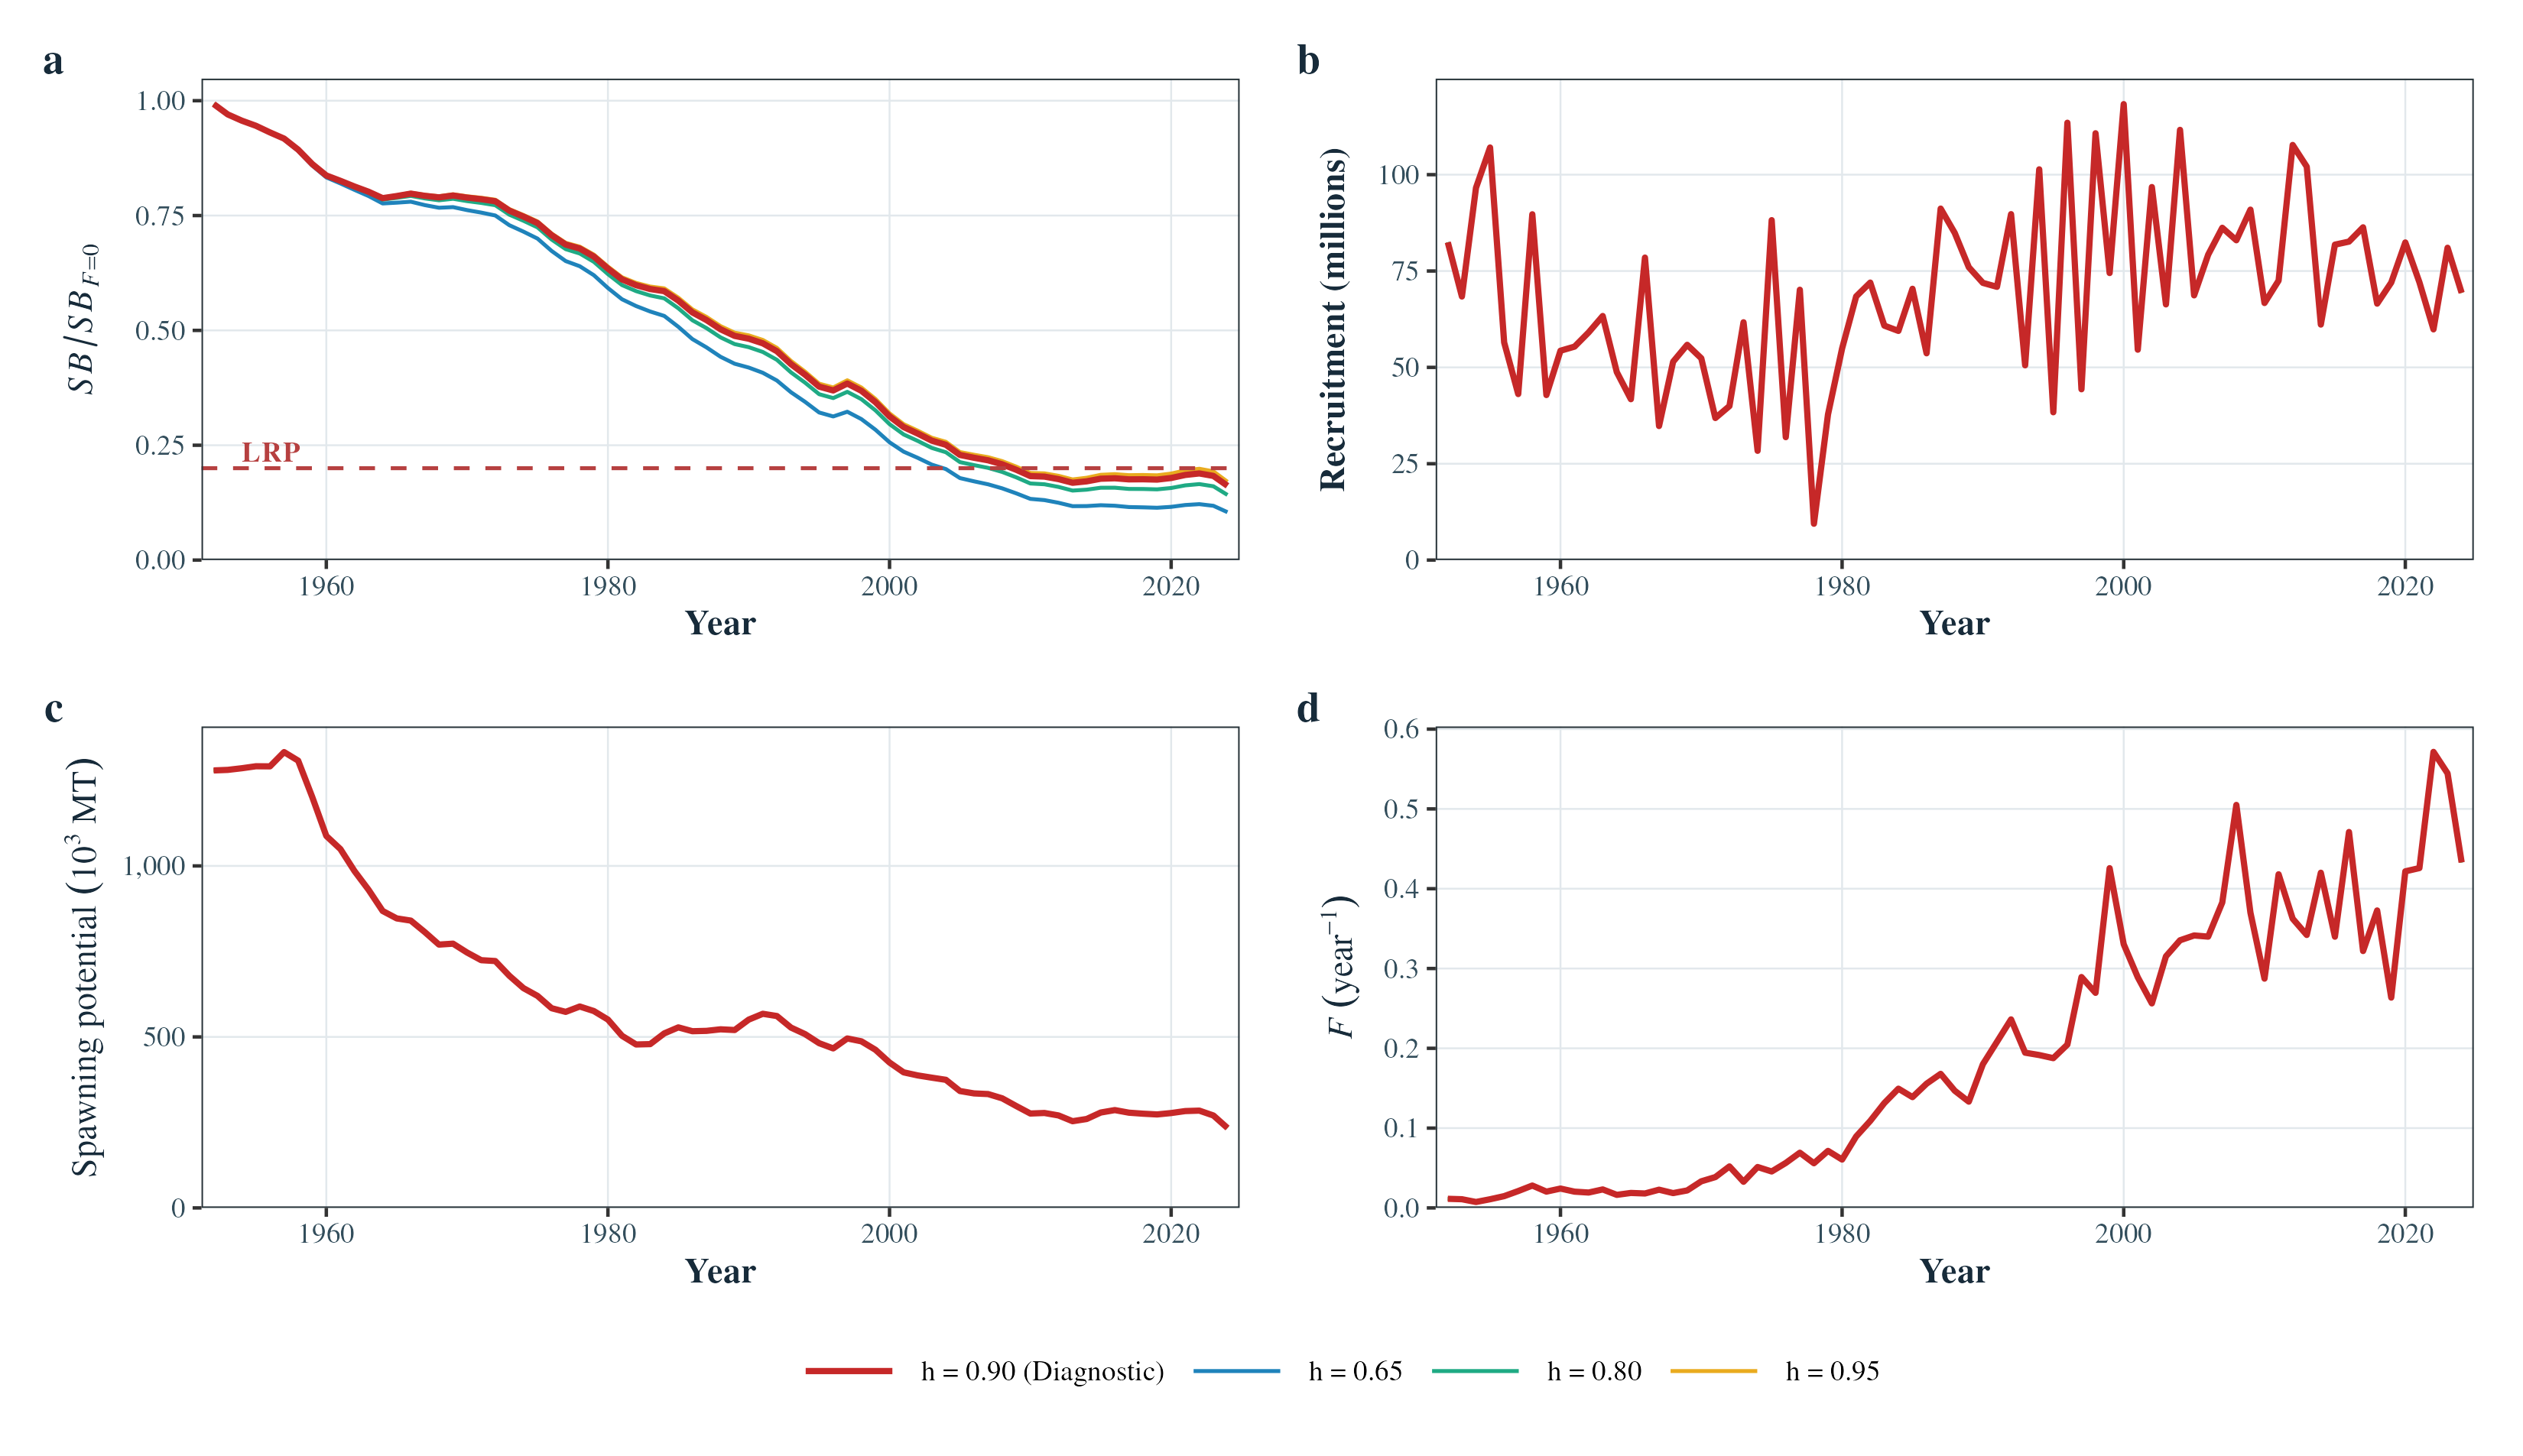
\includegraphics[width=1\linewidth,height=\textheight,keepaspectratio]{figures/sensitivity_steepness.png}

}

\caption{\label{fig-sensitivity-steepness}Estimated dynamic spawning
depletion (Top left) and spawning potential (Bottom left), recruitment
(Top right) and fishing mortality (Bottom right) for the one-off
sensitivities from the 2026 diagnostic model for steepness of the stock
recruitment relationship. Open the
\href{https://pacificcommunity.github.io/ofp-sam-bet-2026-sensitivity/bet-2026-sensitivity-interactive-viewer.html}{interactive
sensitivity viewer}.}

\end{figure}\DIFaddend %

\DIFdelbegin %DIFDELCMD < \begin{figure}[H]
%DIFDELCMD <

%DIFDELCMD < \centering{
%DIFDELCMD <

%DIFDELCMD < 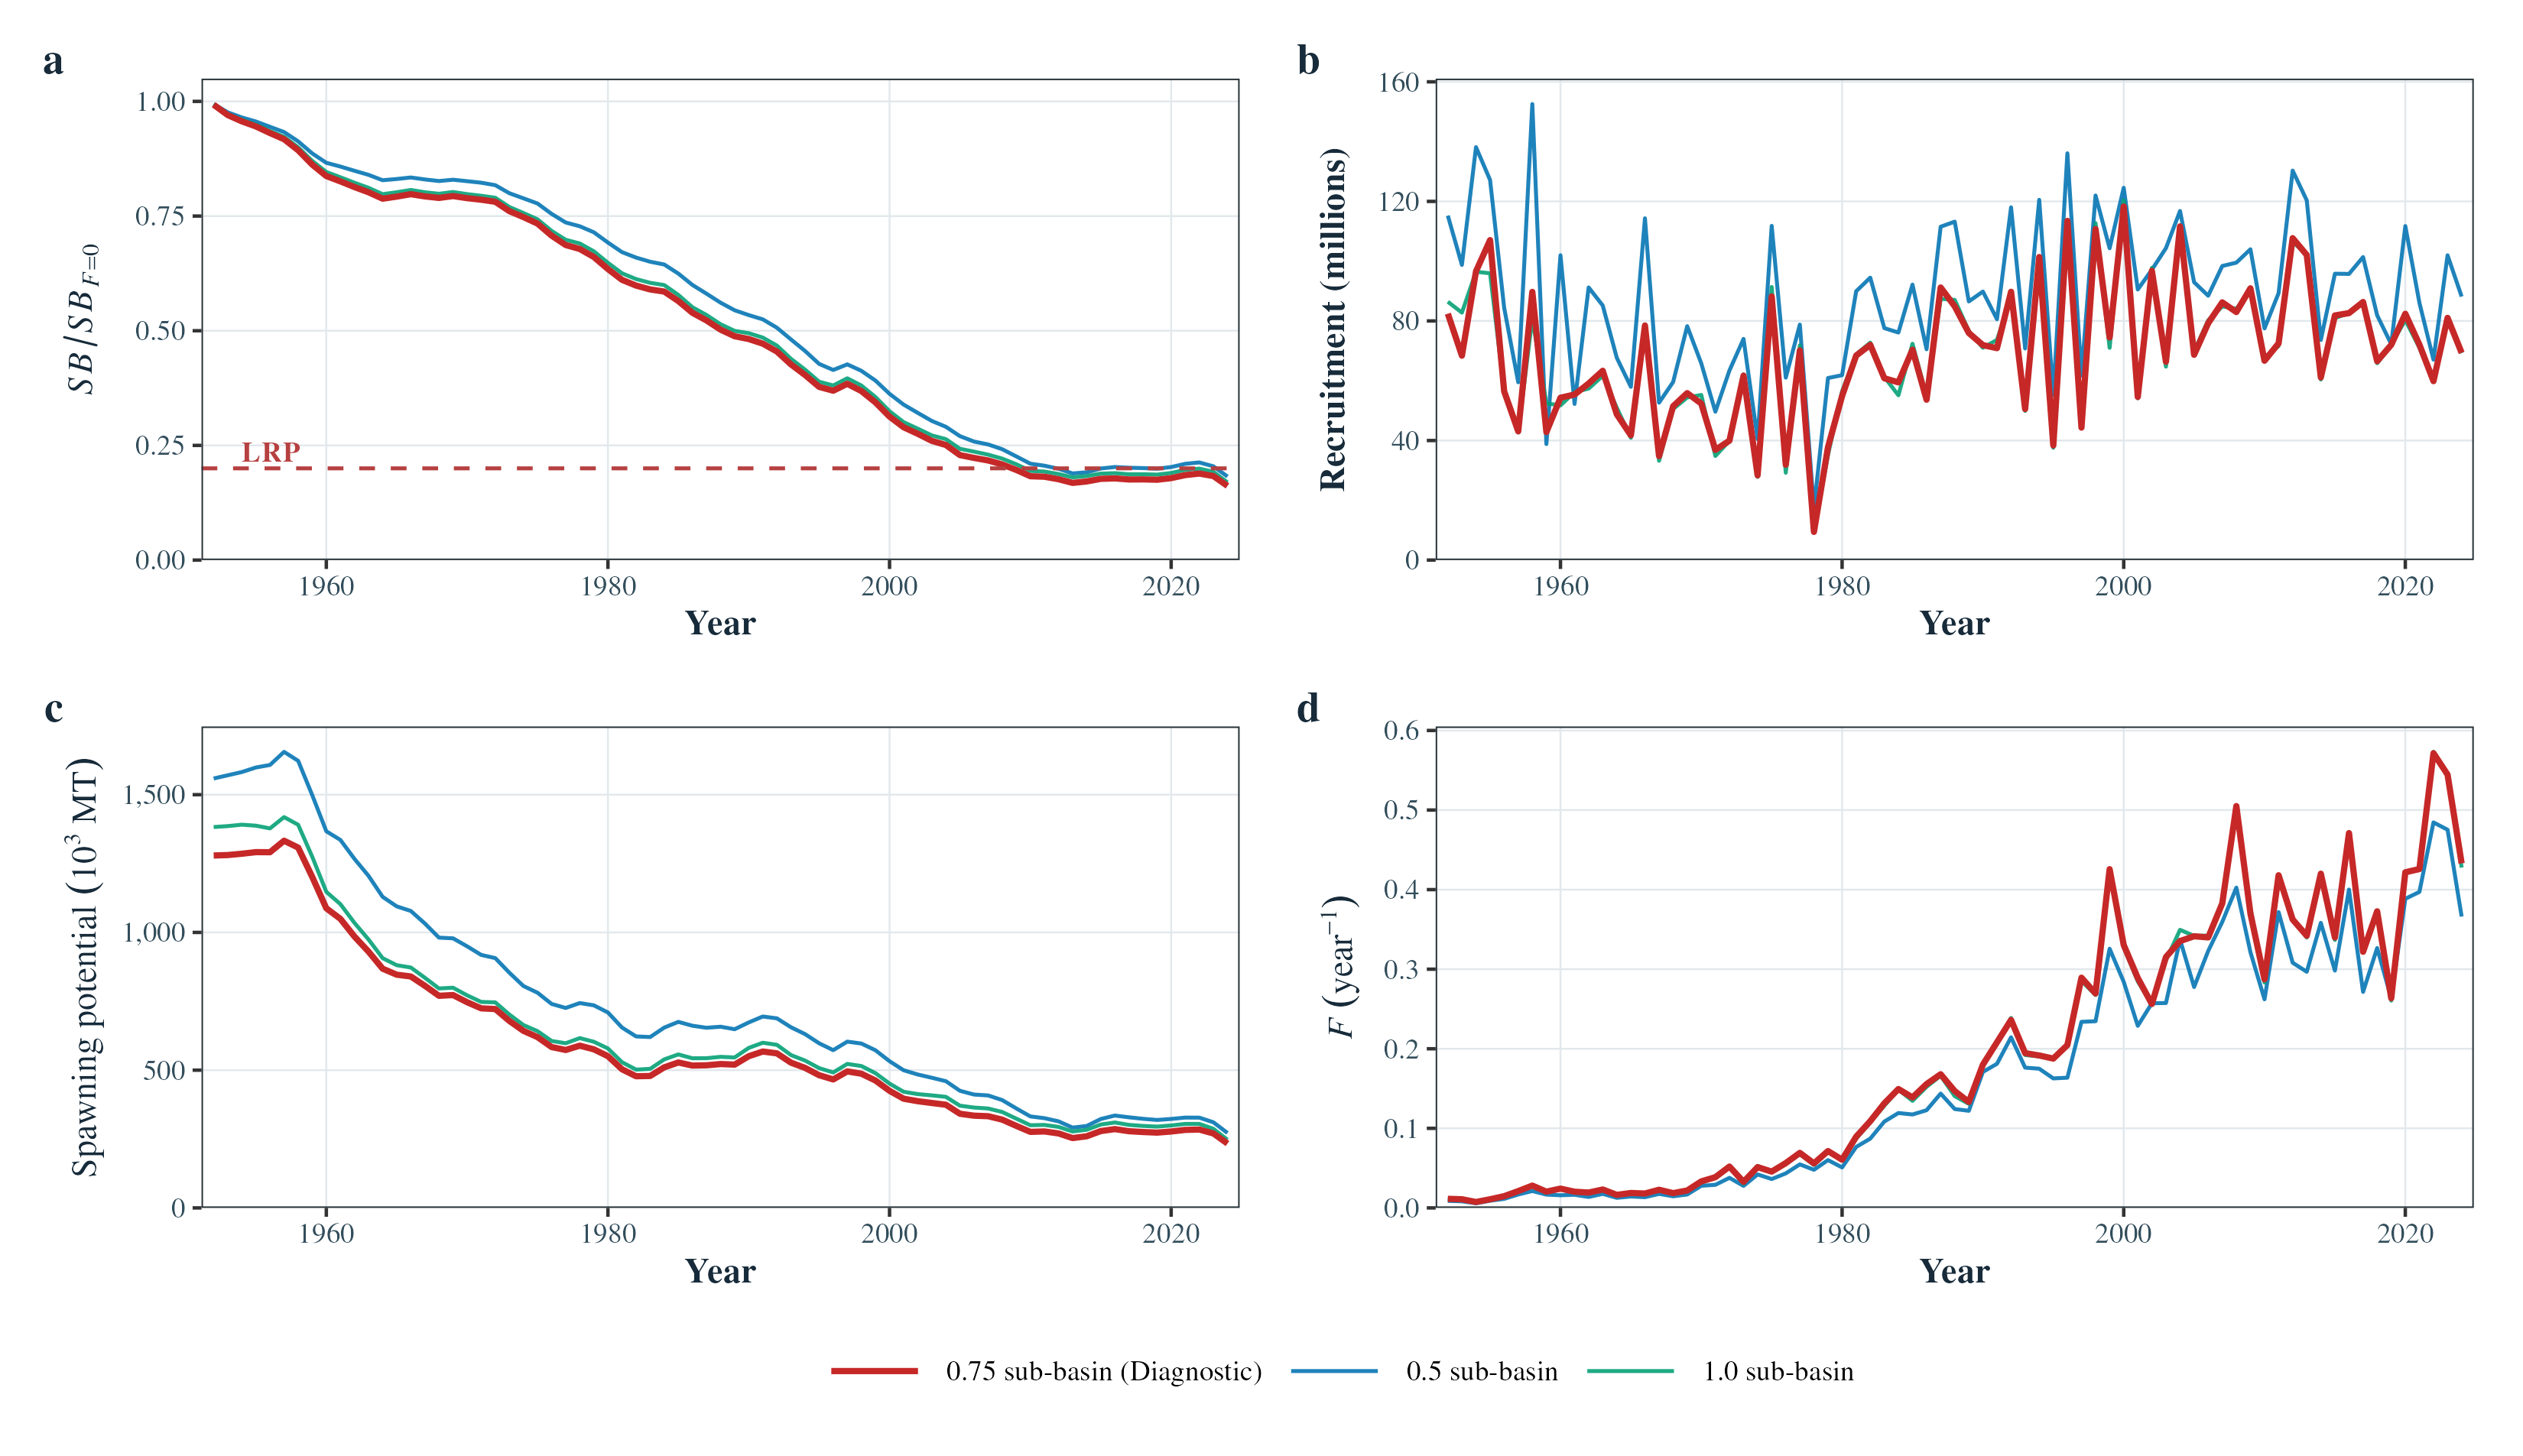
\includegraphics[width=1\linewidth,height=\textheight,keepaspectratio]{figures/sensitivity_CAAL.png}
%DIFDELCMD <

%DIFDELCMD < }
%DIFDELCMD <

%DIFDELCMD < \caption{\label{fig-sensitivity-CAAL}Estimated dynamic spawning
%DIFDELCMD < depletion (Top left) and spawning potential (Bottom left), recruitment
%DIFDELCMD < (Top right) and fishing mortality (Bottom right) for the one-off
%DIFDELCMD < sensitivities from the 2026 diagnostic model for conditional age at
%DIFDELCMD < length (CAAL) data weighting.}
%DIFDELCMD <

%DIFDELCMD < \end{figure}%%%
\DIFdelend \DIFaddbegin \begin{figure}[H]

\centering{

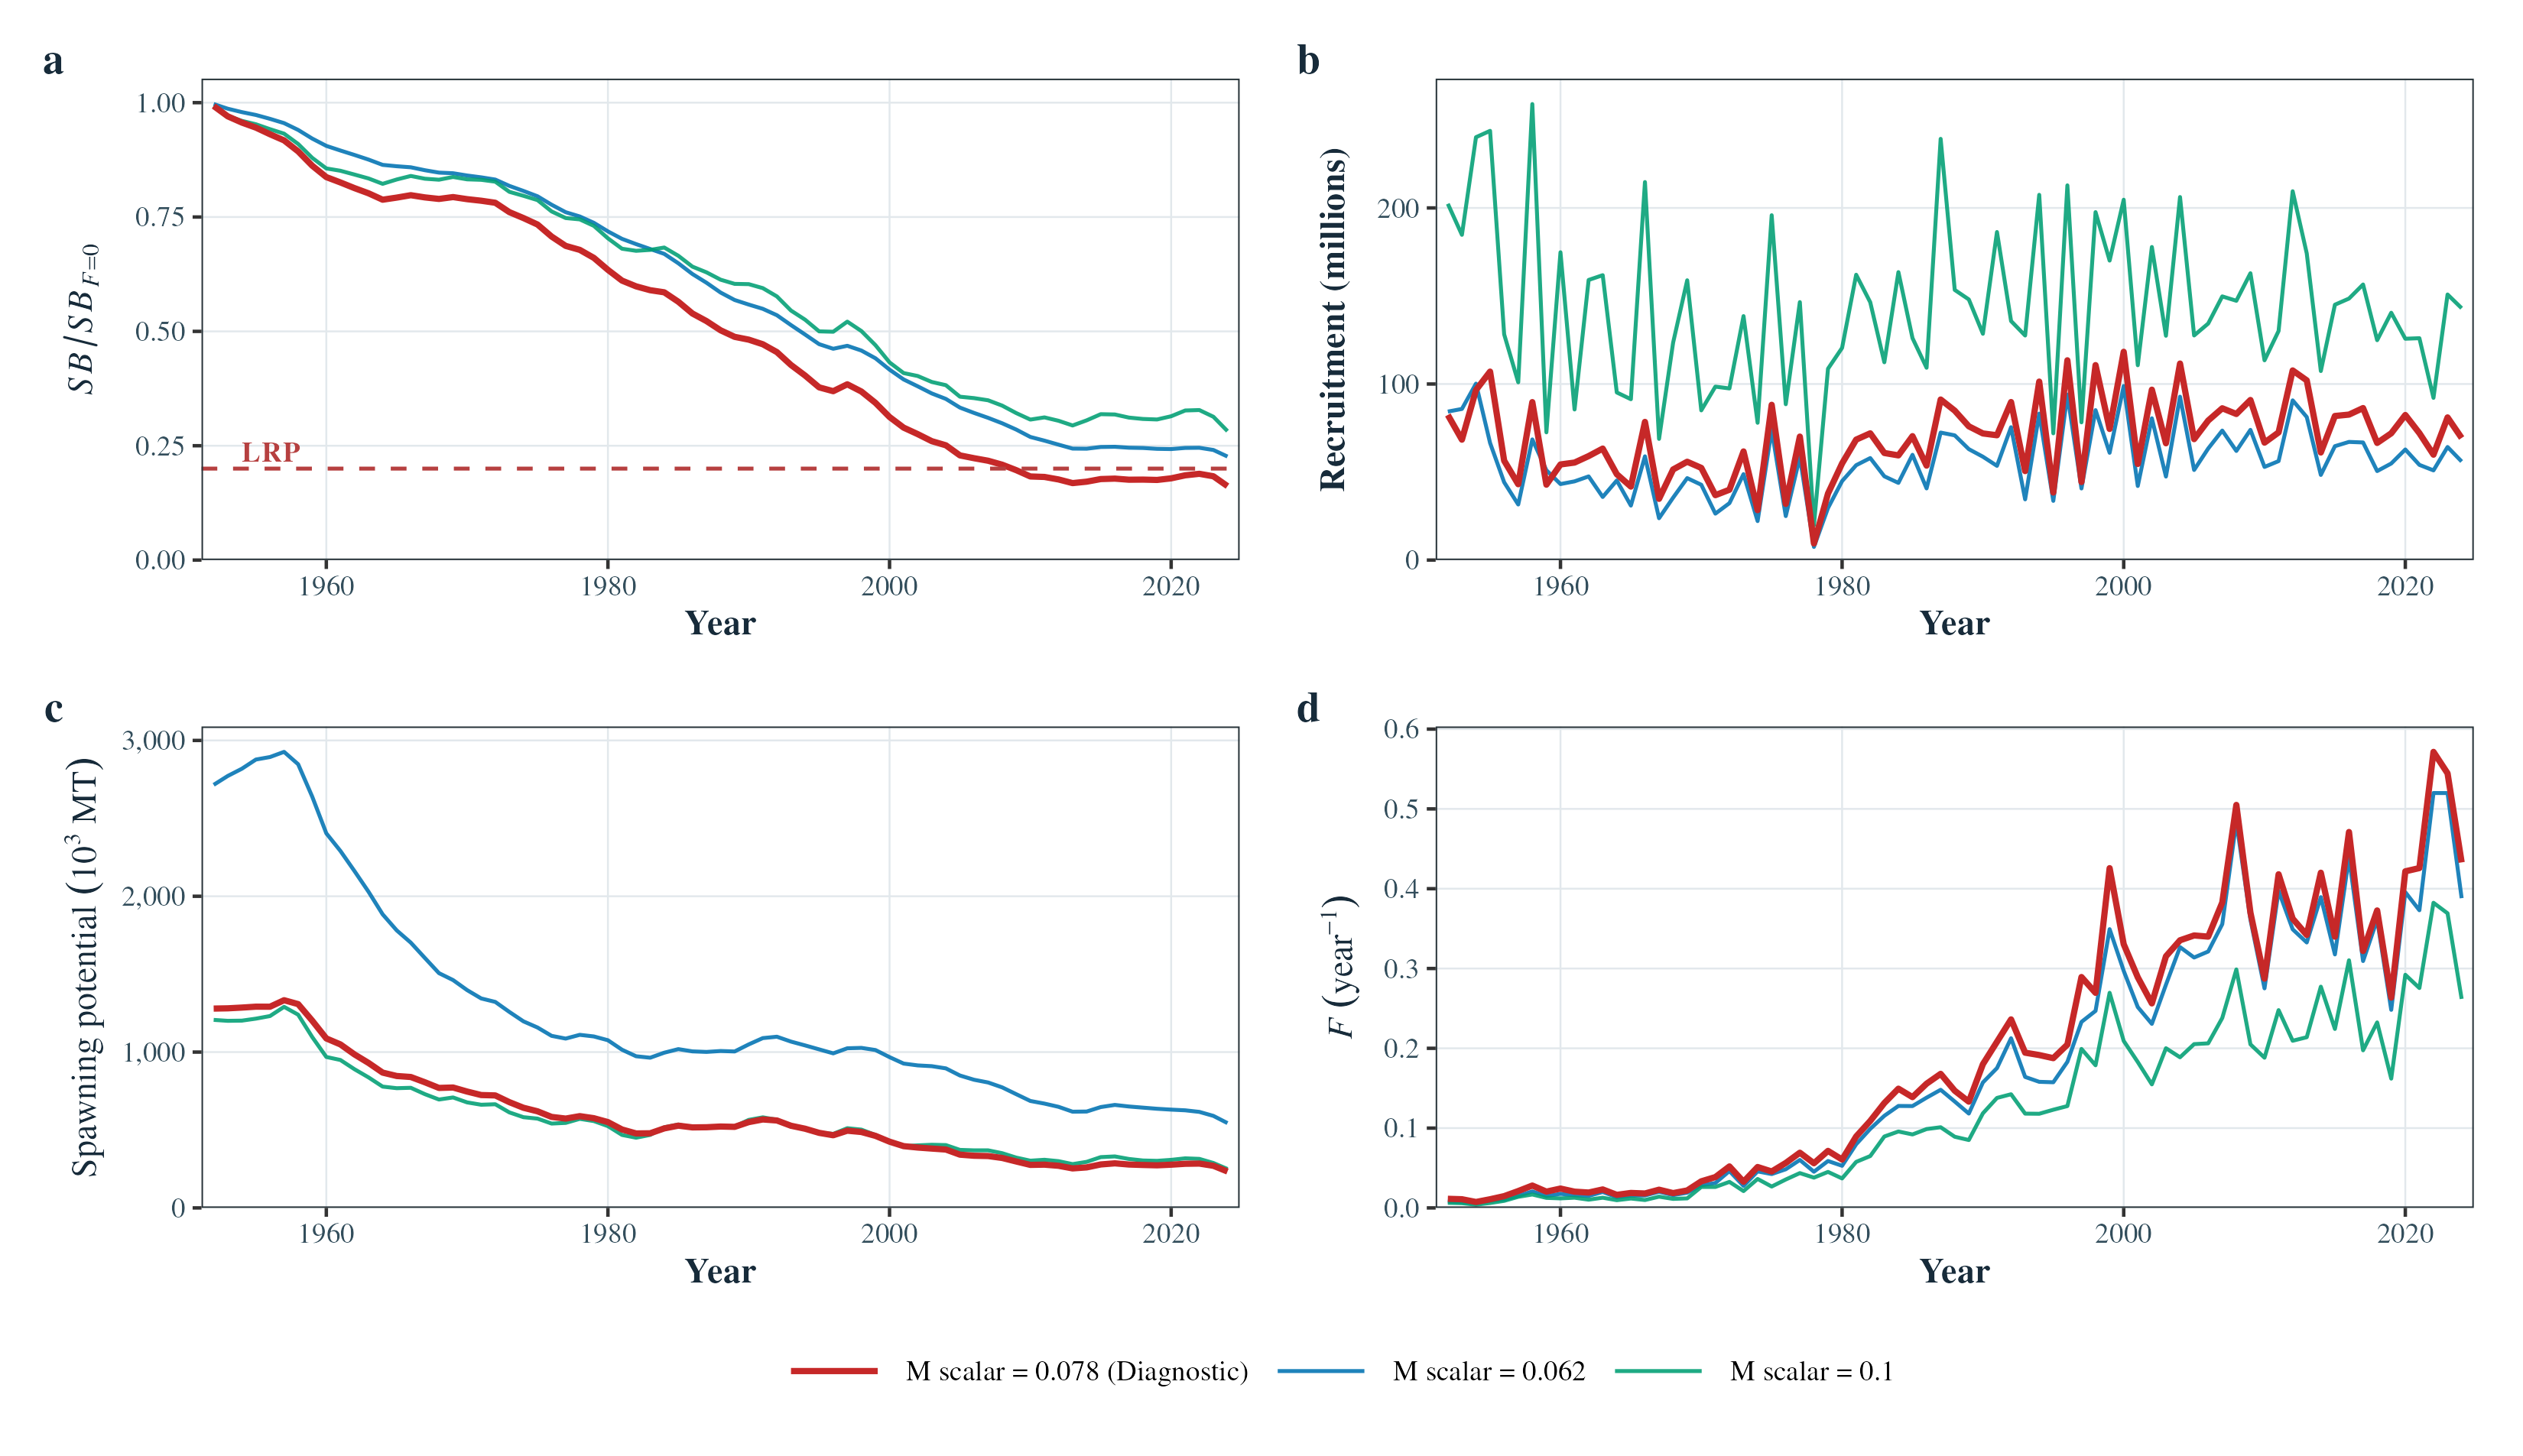
\includegraphics[width=1\linewidth,height=\textheight,keepaspectratio]{figures/sensitivity_natural_mortality.png}

}

\caption{\label{fig-sensitivity-natural-mortality}Estimated dynamic
spawning depletion (Top left) and spawning potential (Bottom left),
recruitment (Top right) and fishing mortality (Bottom right) for the
one-off sensitivities from the 2026 diagnostic model for natural
mortality scale (M at age 40 quarters). Open the
\href{https://pacificcommunity.github.io/ofp-sam-bet-2026-sensitivity/bet-2026-sensitivity-interactive-viewer.html}{interactive
sensitivity viewer}.}

\end{figure}\DIFaddend %

\DIFdelbegin %DIFDELCMD < \begin{figure}[H]
%DIFDELCMD <

%DIFDELCMD < \centering{
%DIFDELCMD <

%DIFDELCMD < 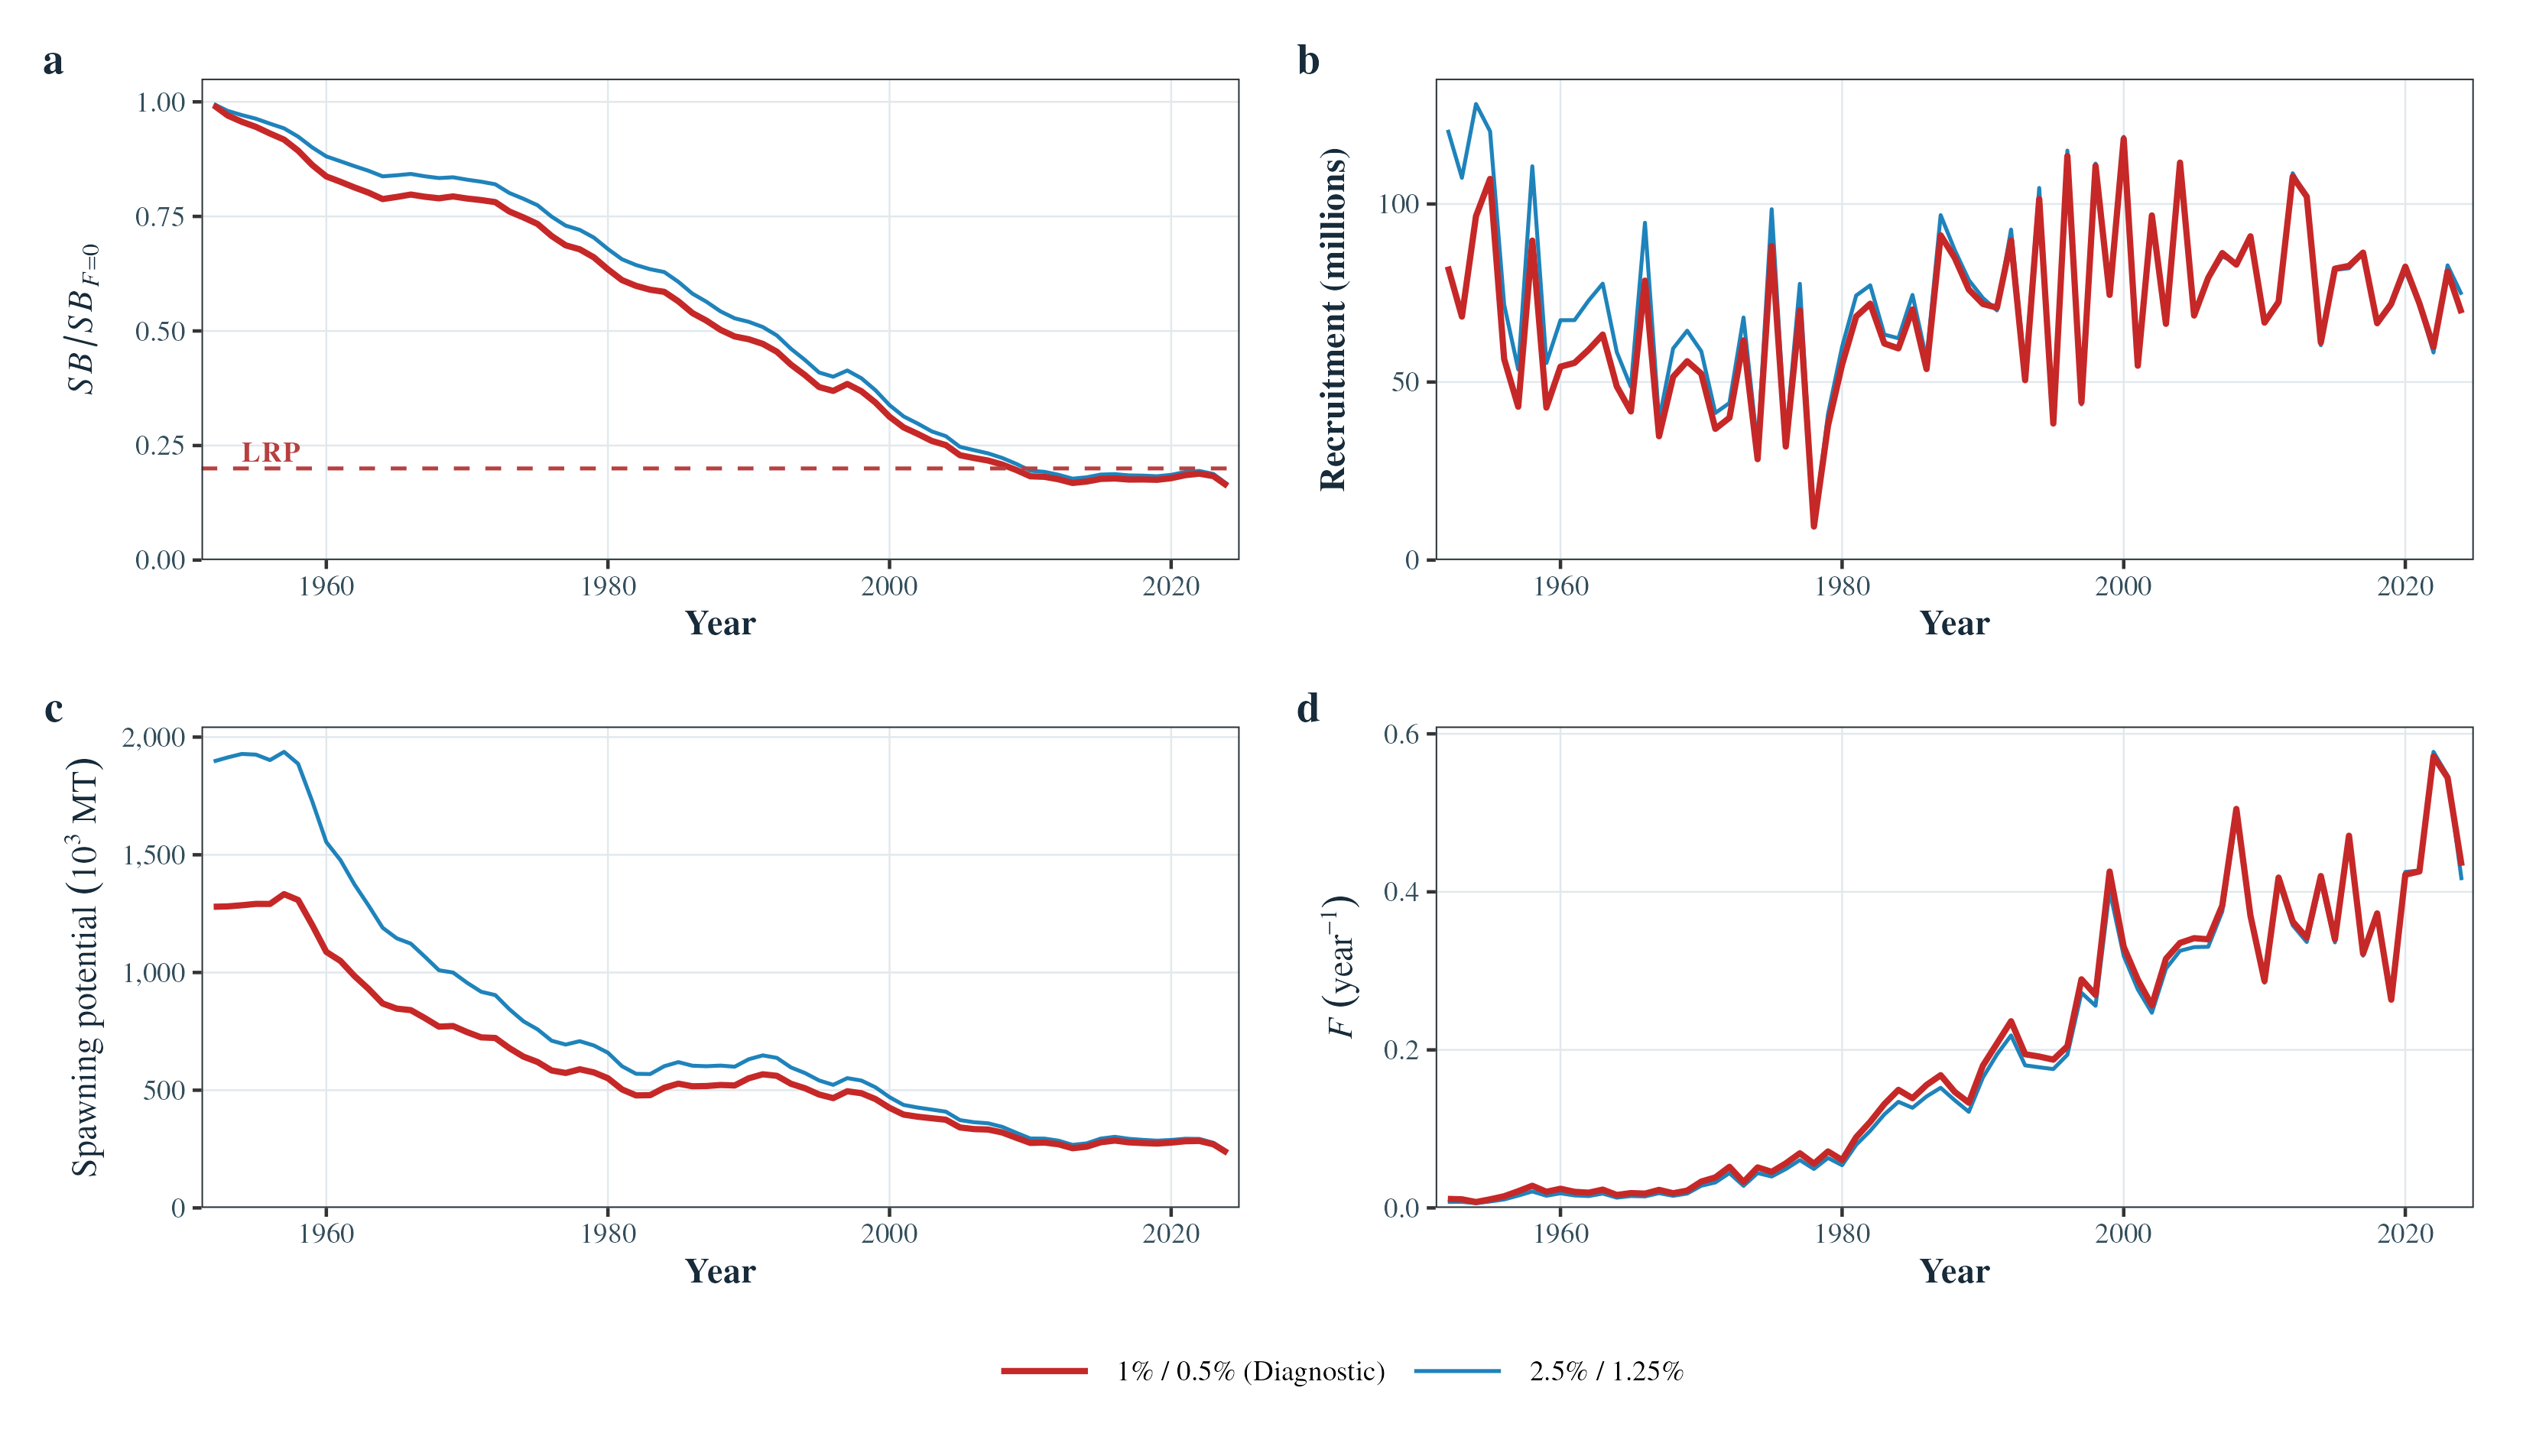
\includegraphics[width=1\linewidth,height=\textheight,keepaspectratio]{figures/sensitivity_effort_creep.png}
%DIFDELCMD <

%DIFDELCMD < }
%DIFDELCMD <

%DIFDELCMD < \caption{\label{fig-sensitivity-effort-creep}Estimated dynamic spawning
%DIFDELCMD < depletion (Top left) and spawning potential (Bottom left), recruitment
%DIFDELCMD < (Top right) and fishing mortality (Bottom right) for the one-off
%DIFDELCMD < sensitivities from the 2026 diagnostic model for effort creep adjustment
%DIFDELCMD < to CPUE indices.}
%DIFDELCMD <

%DIFDELCMD < \end{figure}%%%
\DIFdelend \DIFaddbegin \begin{figure}[H]

\centering{

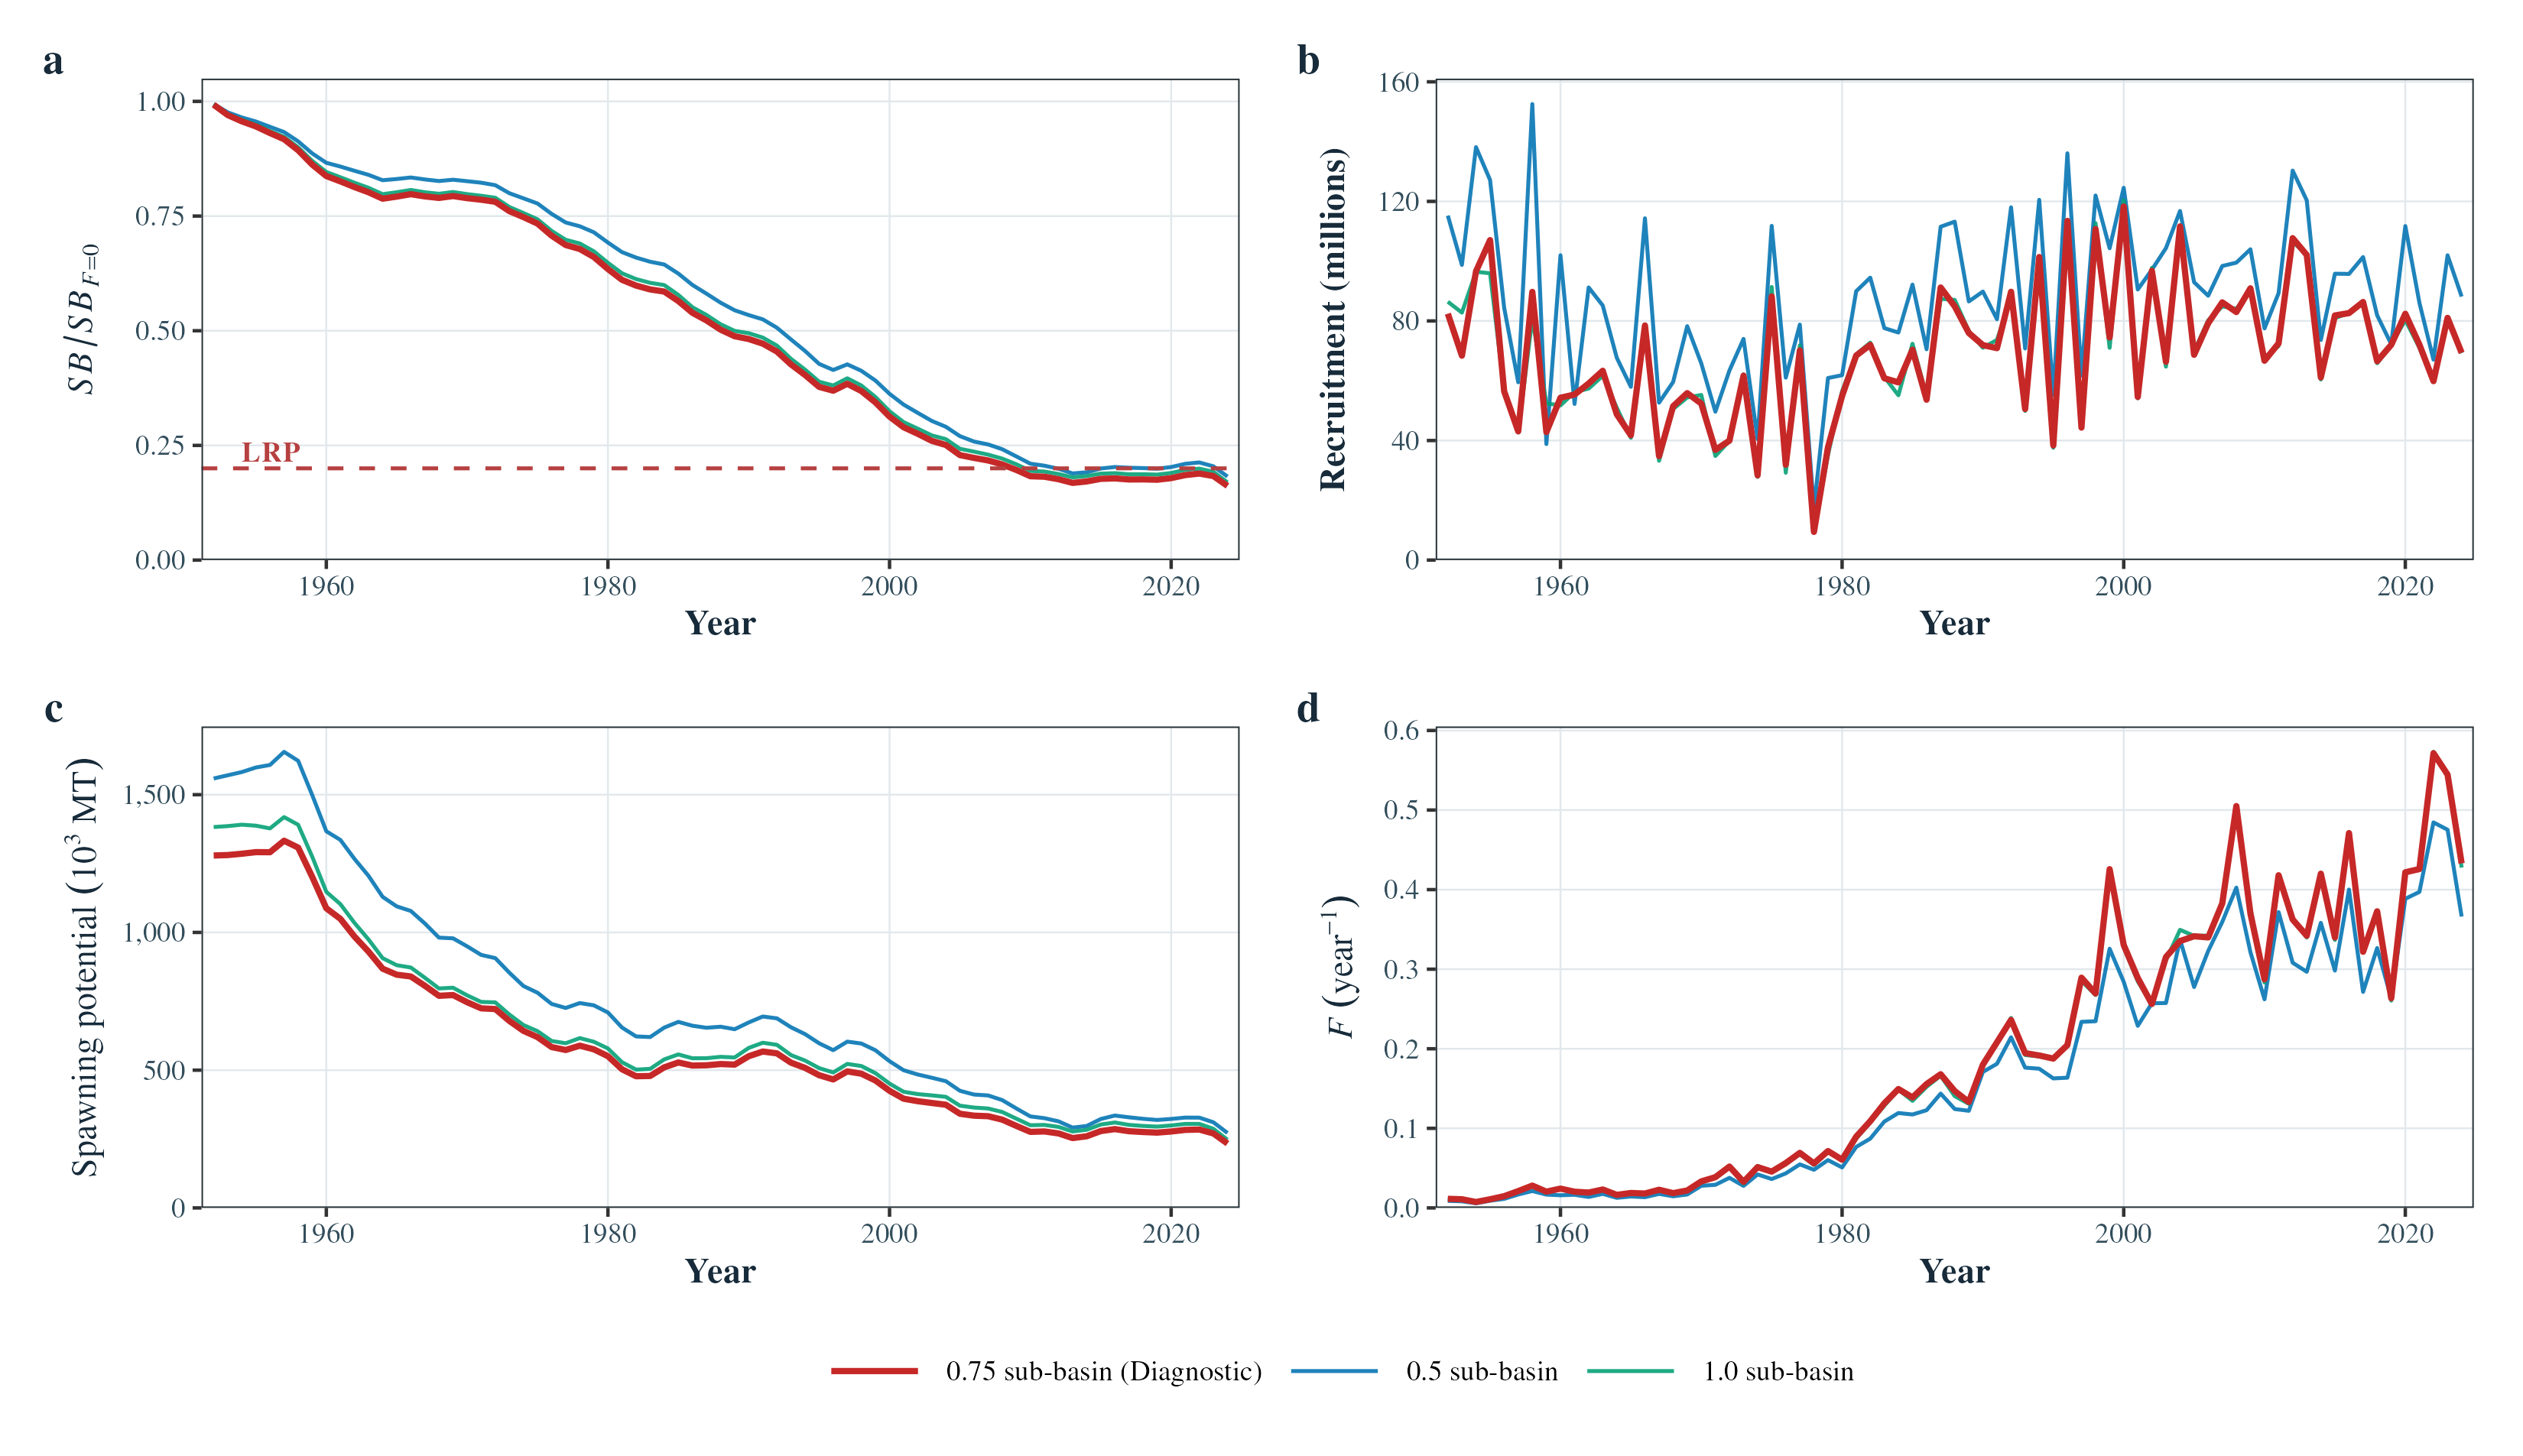
\includegraphics[width=1\linewidth,height=\textheight,keepaspectratio]{figures/sensitivity_CAAL.png}

}

\caption{\label{fig-sensitivity-CAAL}Estimated dynamic spawning
depletion (Top left) and spawning potential (Bottom left), recruitment
(Top right) and fishing mortality (Bottom right) for the one-off
sensitivities from the 2026 diagnostic model for conditional age at
length (CAAL) data weighting. Open the
\href{https://pacificcommunity.github.io/ofp-sam-bet-2026-sensitivity/bet-2026-sensitivity-interactive-viewer.html}{interactive
sensitivity viewer}.}

\end{figure}\DIFaddend %

\DIFdelbegin %DIFDELCMD < \begin{figure}[H]
%DIFDELCMD <

%DIFDELCMD < \centering{
%DIFDELCMD <

%DIFDELCMD < 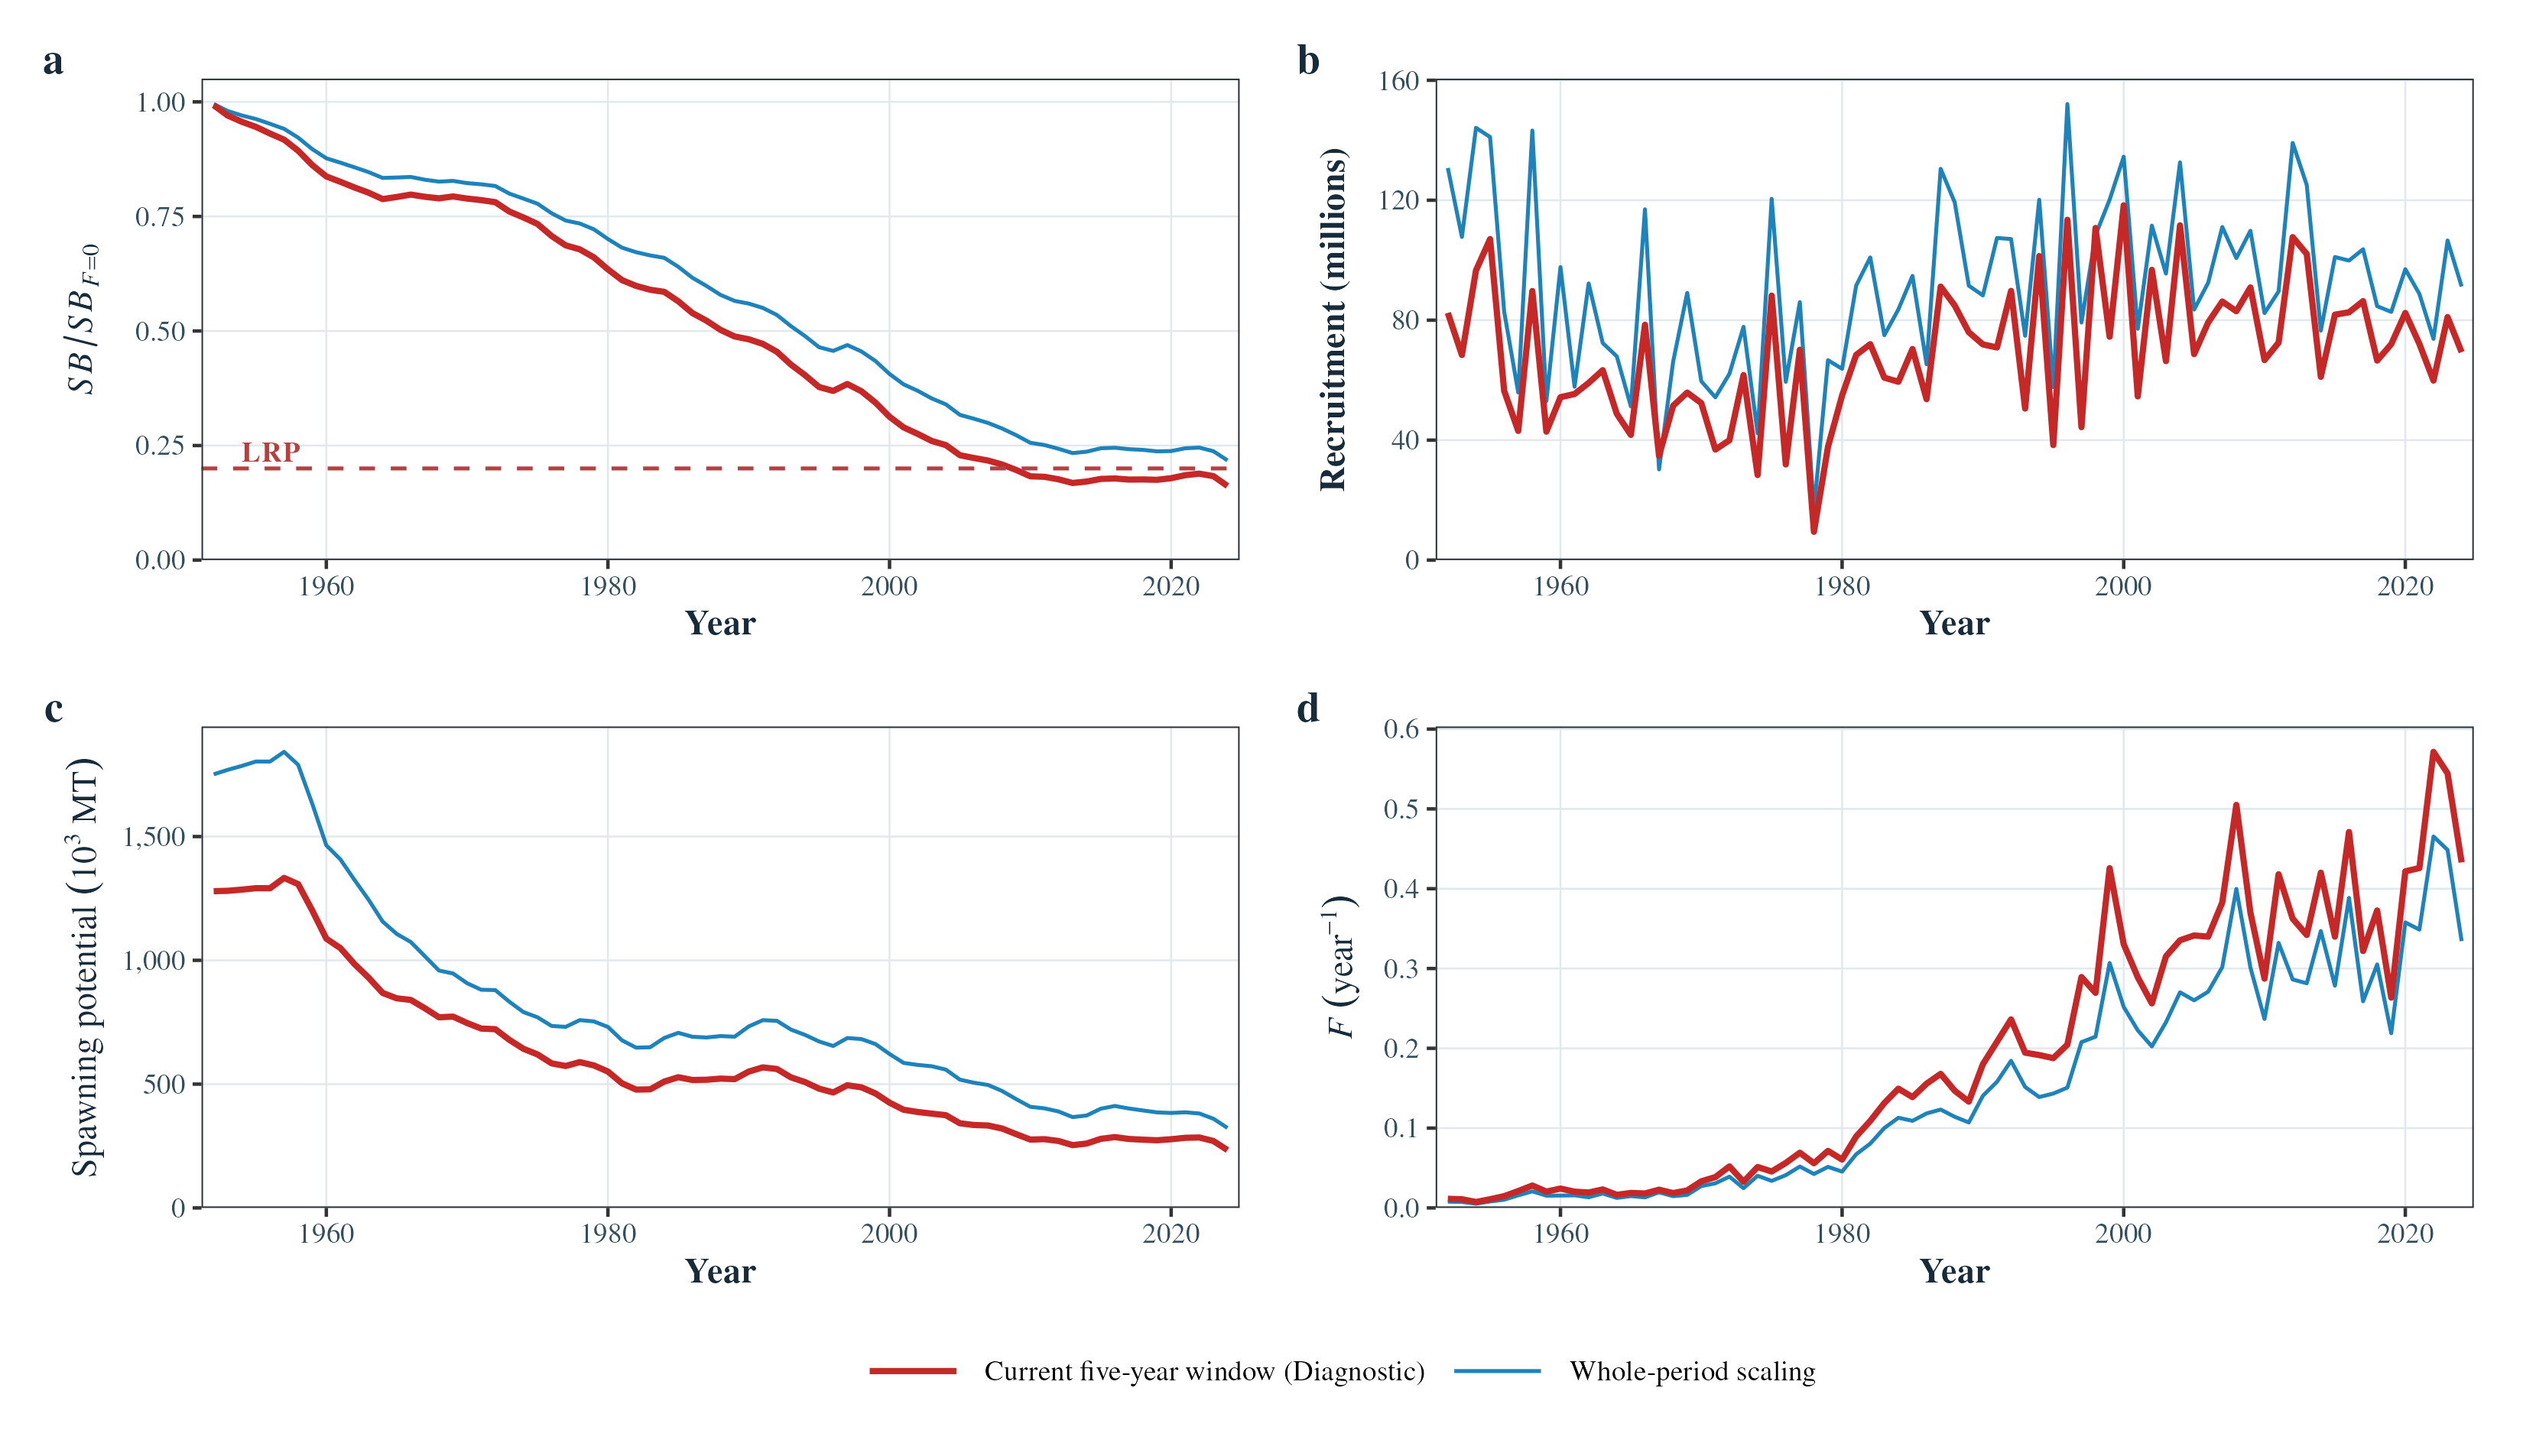
\includegraphics[width=1\linewidth,height=\textheight,keepaspectratio]{figures/sensitivity_regional_scaling.png}
%DIFDELCMD <

%DIFDELCMD < }
%DIFDELCMD <

%DIFDELCMD < \caption{\label{fig-sensitivity-regional-scaling}Estimated dynamic
%DIFDELCMD < spawning depletion (Top left) and spawning potential (Bottom left),
%DIFDELCMD < recruitment (Top right) and fishing mortality (Bottom right) for the
%DIFDELCMD < one-off sensitivities from the 2026 diagnostic model for effort creep
%DIFDELCMD < adjustment to CPUE indices the time period used form the global CPUE
%DIFDELCMD < anlysis for the regional scaling penalty. Current five year window
%DIFDELCMD < refers to the shorter early time period of maximum coverage used in the
%DIFDELCMD < diagnostic case (i.e 1965-1969, as recommended in PAW), whole period in
%DIFDELCMD < full time series, 1952-2024.}
%DIFDELCMD <

%DIFDELCMD < \end{figure}%%%
\DIFdelend \DIFaddbegin \begin{figure}[H]

\centering{

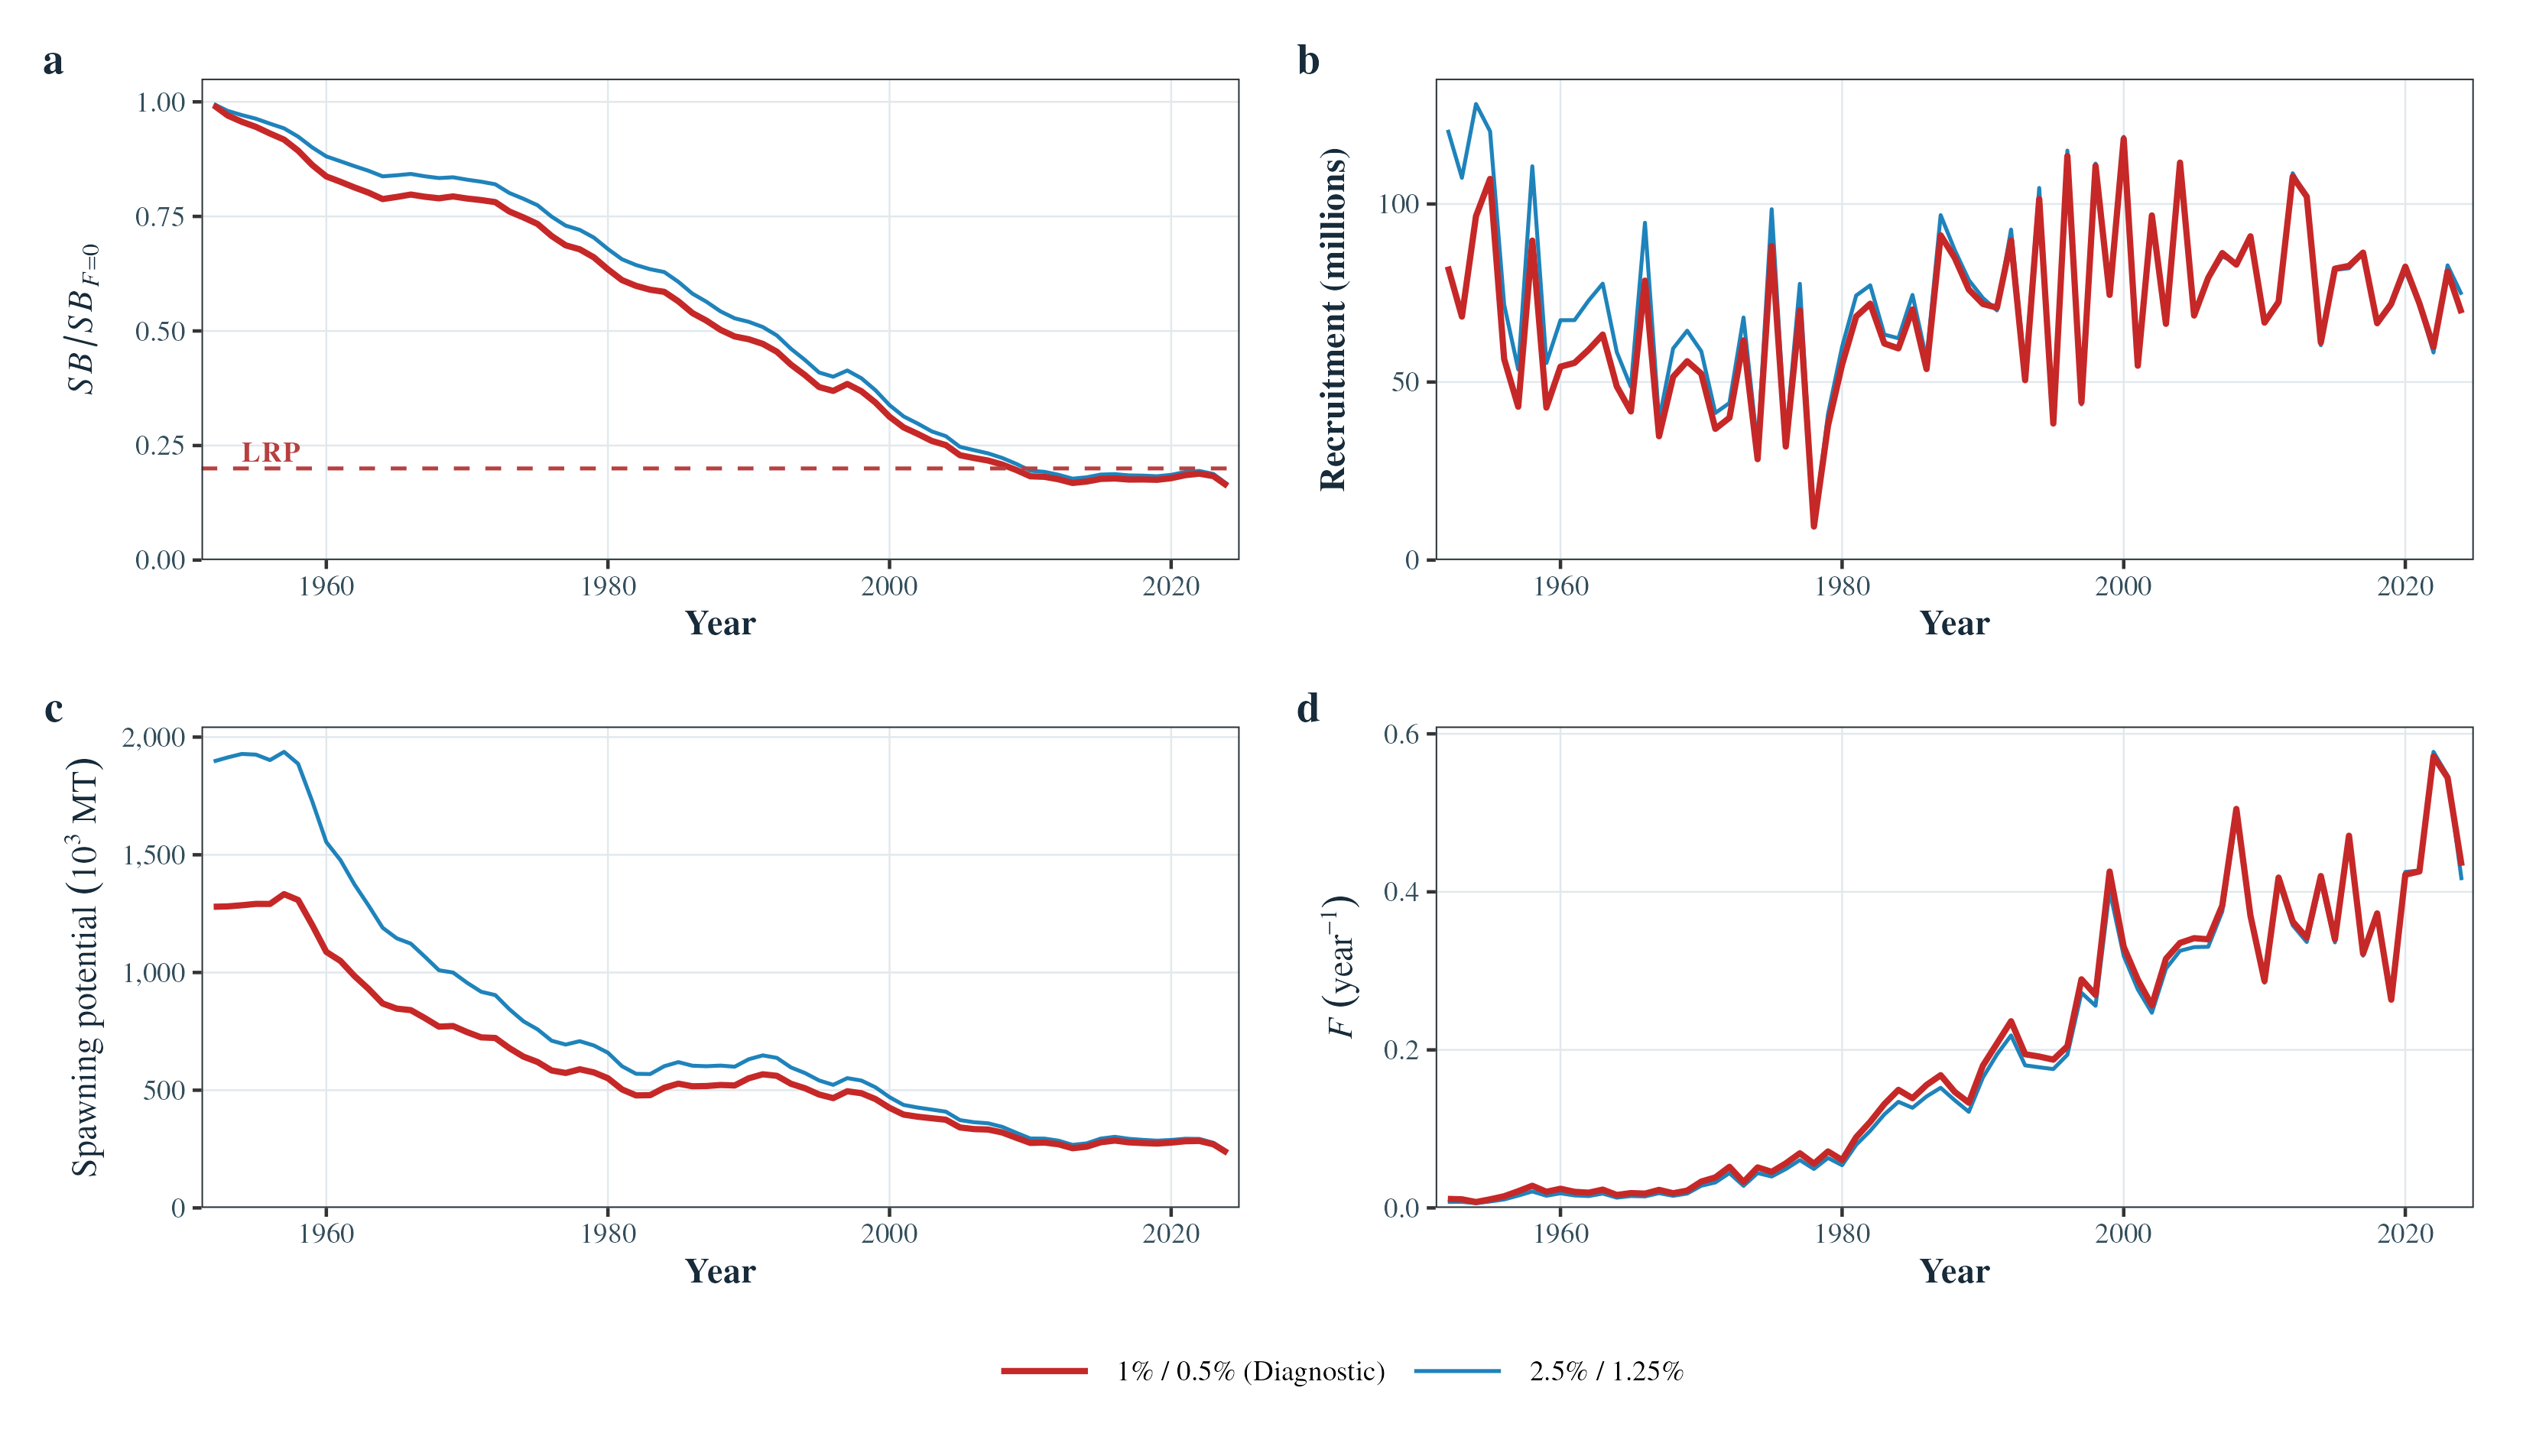
\includegraphics[width=1\linewidth,height=\textheight,keepaspectratio]{figures/sensitivity_effort_creep.png}

}

\caption{\label{fig-sensitivity-effort-creep}Estimated dynamic spawning
depletion (Top left) and spawning potential (Bottom left), recruitment
(Top right) and fishing mortality (Bottom right) for the one-off
sensitivities from the 2026 diagnostic model for effort creep adjustment
to CPUE indices. Open the
\href{https://pacificcommunity.github.io/ofp-sam-bet-2026-sensitivity/bet-2026-sensitivity-interactive-viewer.html}{interactive
sensitivity viewer}.}

\end{figure}\DIFaddend %

\DIFdelbegin %DIFDELCMD < \begin{figure}[H]
%DIFDELCMD <

%DIFDELCMD < \centering{
%DIFDELCMD <

%DIFDELCMD < 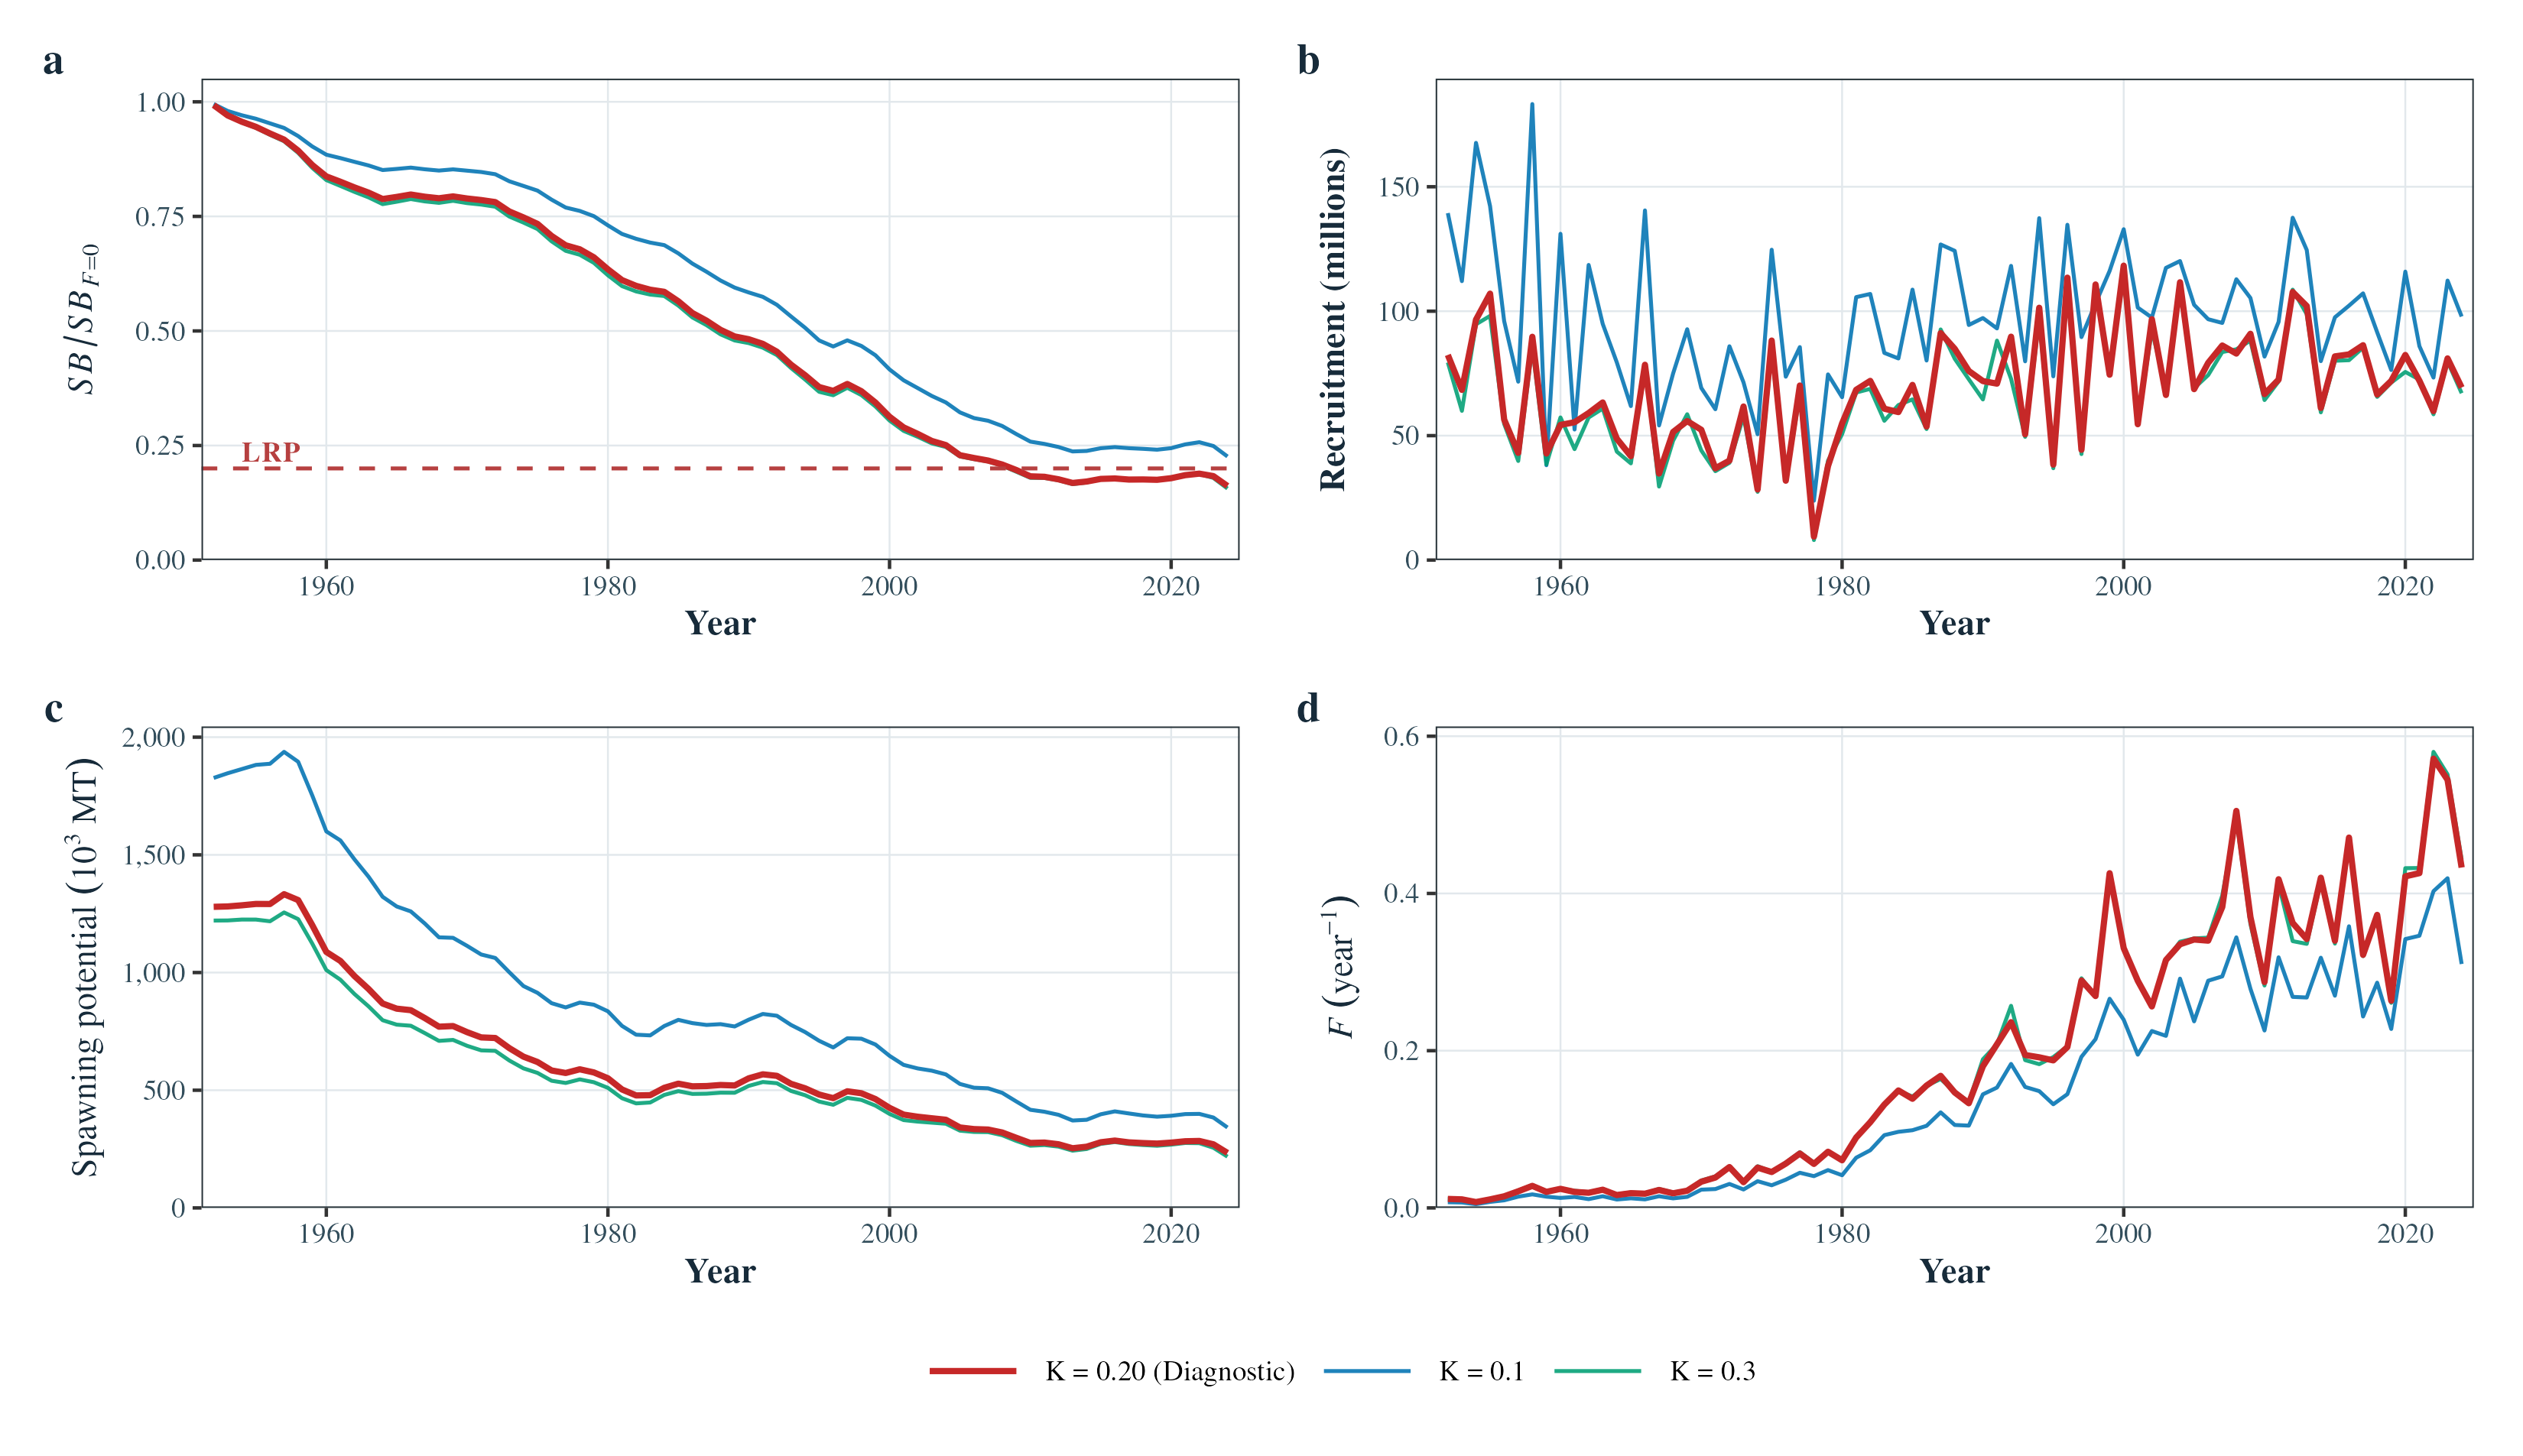
\includegraphics[width=1\linewidth,height=\textheight,keepaspectratio]{figures/sensitivity_tag_mixing_periods_Kstatistic_cutoff.png}
%DIFDELCMD <

%DIFDELCMD < }
%DIFDELCMD <

%DIFDELCMD < \caption{\label{fig-sensitivity-tag-mixing-periods-Kstatistic-cutoff}Estimated
%DIFDELCMD < dynamic spawning depletion (Top left) and spawning potential (Bottom
%DIFDELCMD < left), recruitment (Top right) and fishing mortality (Bottom right) for
%DIFDELCMD < the one-off sensitivities from the 2026 diagnostic model on the
%DIFDELCMD < K-statistic for assigning release group specific mixing periods - higher
%DIFDELCMD < value assume less conservative shorter mixing periods, lower value
%DIFDELCMD < assume more conservative longer mixing periods.}
%DIFDELCMD <

%DIFDELCMD < \end{figure}%%%
\DIFdelend \DIFaddbegin \begin{figure}[H]

\centering{

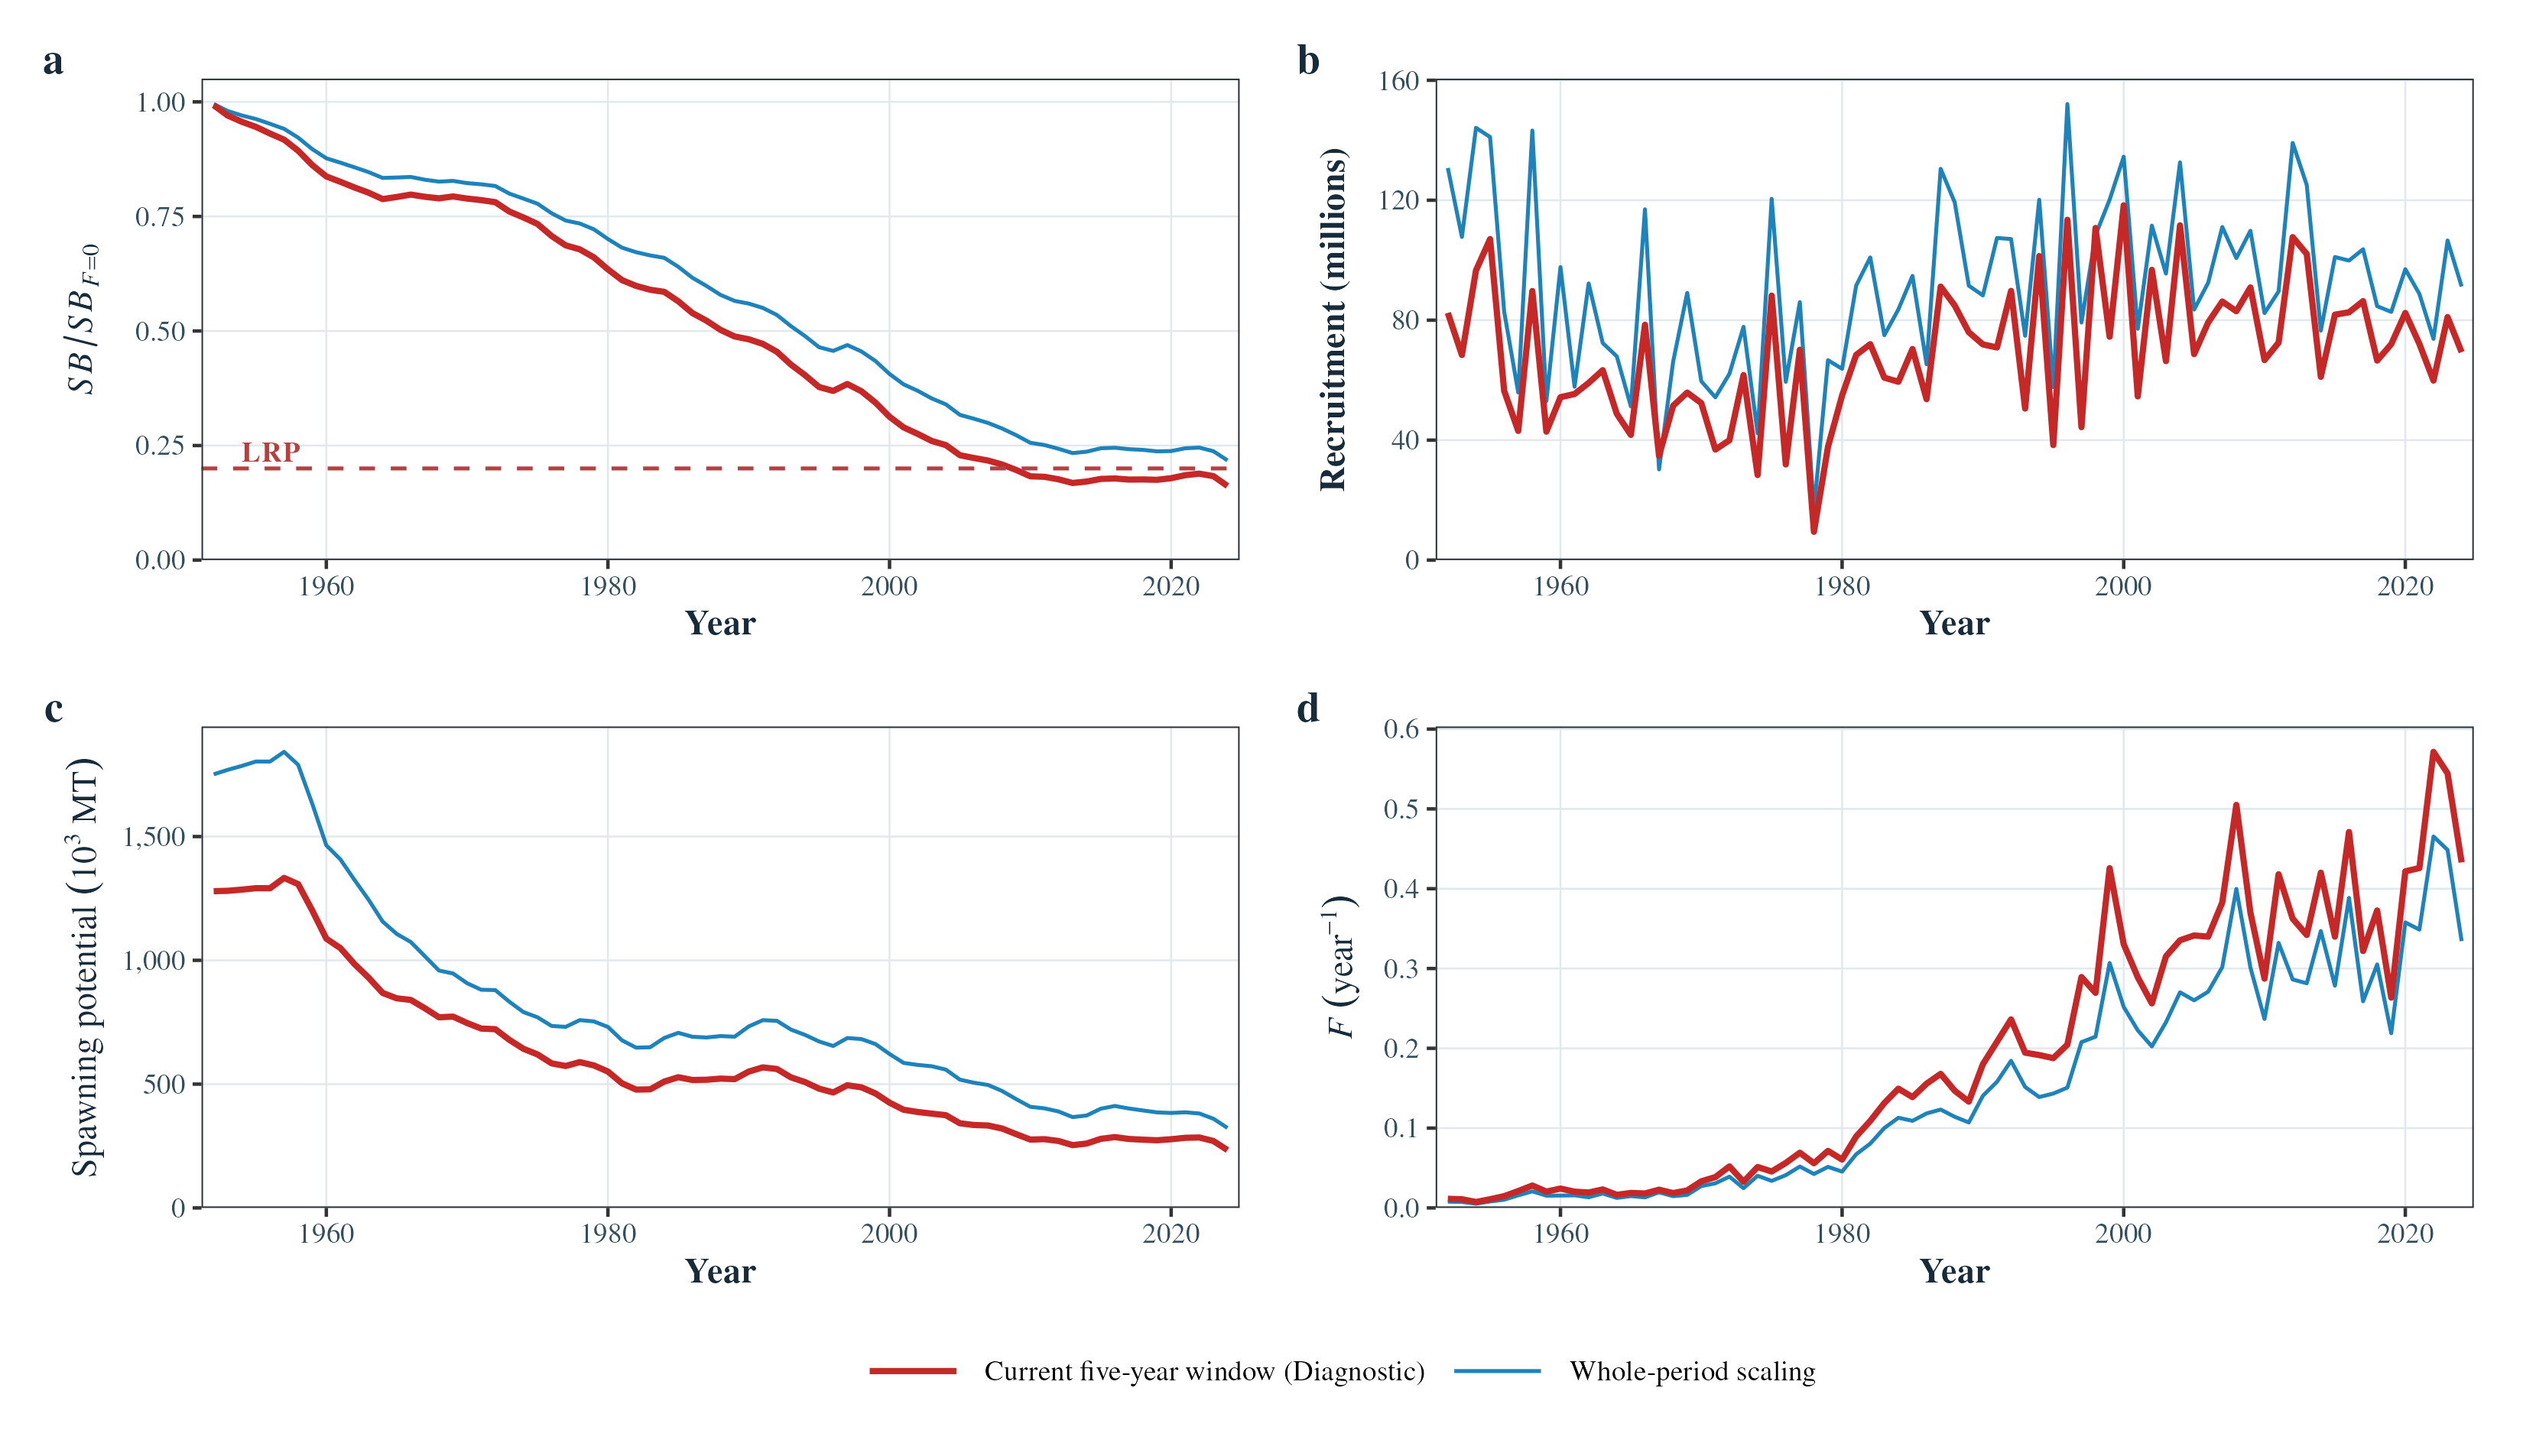
\includegraphics[width=1\linewidth,height=\textheight,keepaspectratio]{figures/sensitivity_regional_scaling.png}

}

\caption{\label{fig-sensitivity-regional-scaling}Dynamic spawning
depletion (top left), spawning potential (bottom left), recruitment (top
right) and fishing mortality (bottom right) for one-off sensitivities to
the global-CPUE period used in the regional-scaling penalty. The
diagnostic model uses the 1965--1969 period of broad spatial coverage
recommended by PAW; the alternative uses the full 1952--2024 series.
Open the
\href{https://pacificcommunity.github.io/ofp-sam-bet-2026-sensitivity/bet-2026-sensitivity-interactive-viewer.html}{interactive
sensitivity viewer}.}

\end{figure}\DIFaddend %

\DIFdelbegin %DIFDELCMD < \begin{figure}[H]
%DIFDELCMD <

%DIFDELCMD < \centering{
%DIFDELCMD <

%DIFDELCMD < 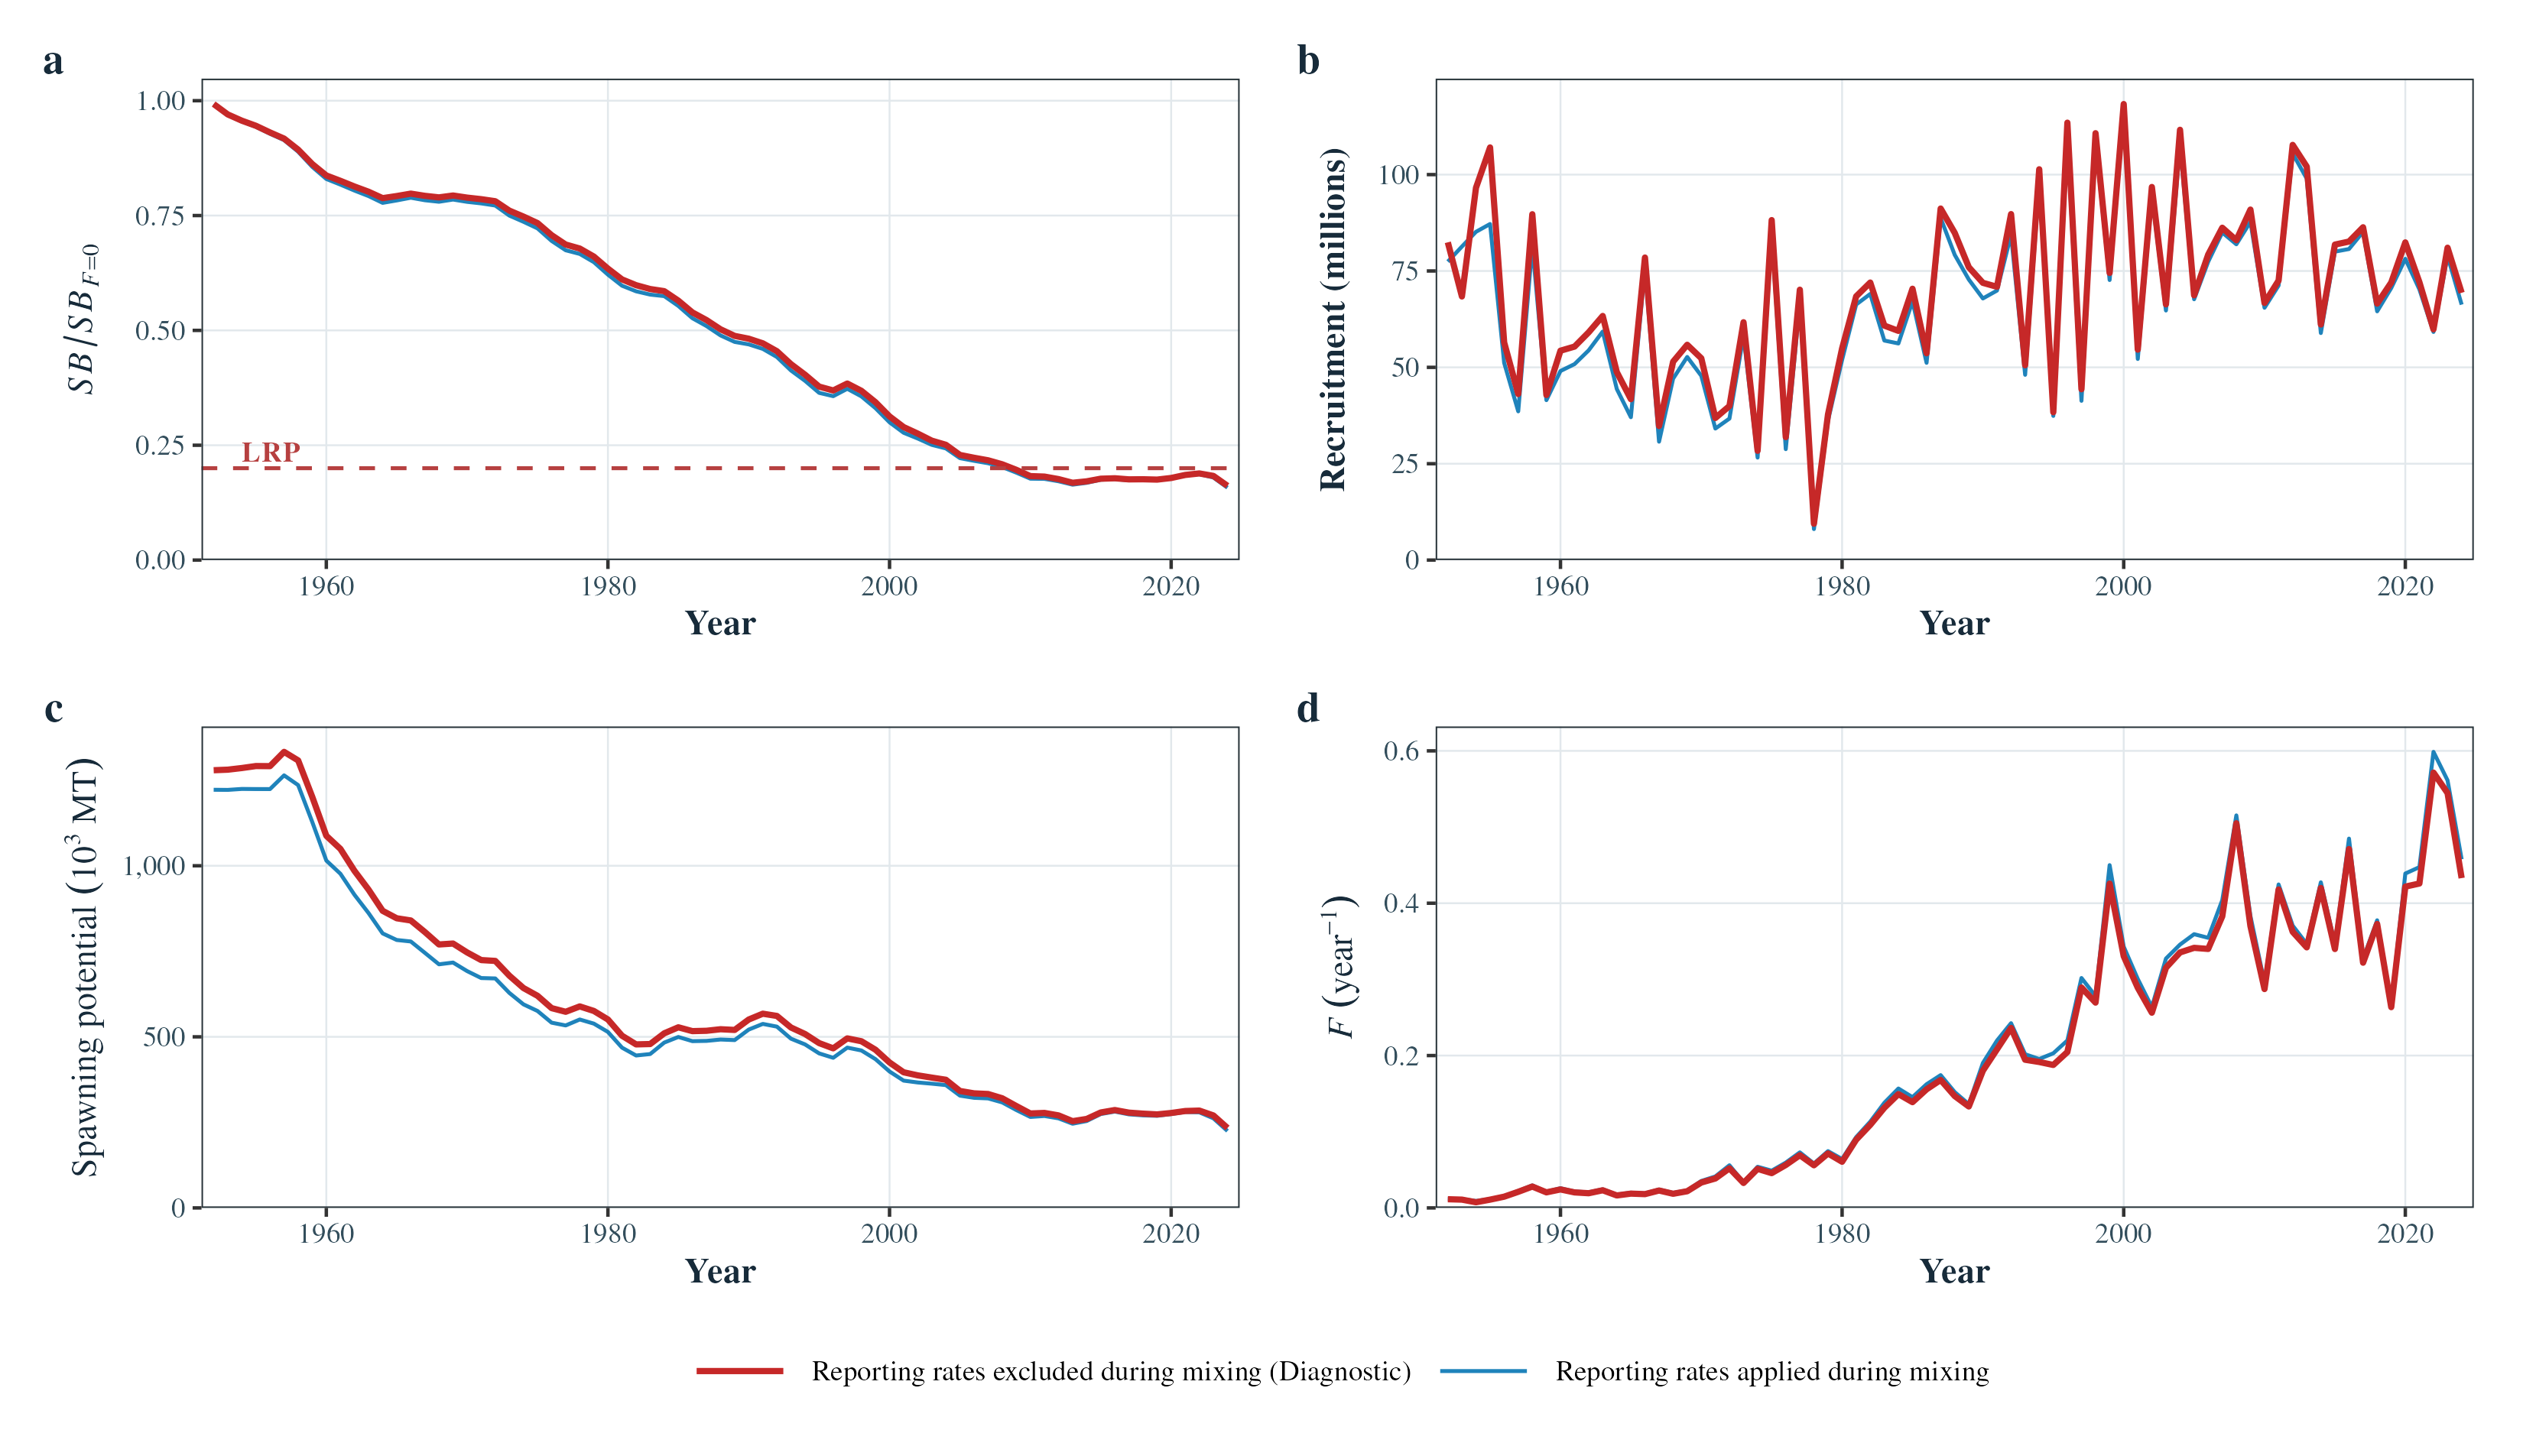
\includegraphics[width=1\linewidth,height=\textheight,keepaspectratio]{figures/sensitivity_premixing_tag_reporting_rate.png}
%DIFDELCMD <

%DIFDELCMD < }
%DIFDELCMD <

%DIFDELCMD < \caption{\label{fig-sensitivity-premixing-tag-reporting-rate}Estimated
%DIFDELCMD < dynamic spawning depletion (Top left) and spawning potential (Bottom
%DIFDELCMD < left), recruitment (Top right) and fishing mortality (Bottom right) for
%DIFDELCMD < the one-off sensitivities from the 2026 diagnostic model on the option
%DIFDELCMD < to activate or deactivate reporting rate adjustments during tag mixing
%DIFDELCMD < periods.}
%DIFDELCMD <

%DIFDELCMD < \end{figure}%%%
\DIFdelend \DIFaddbegin \begin{figure}[H]

\centering{

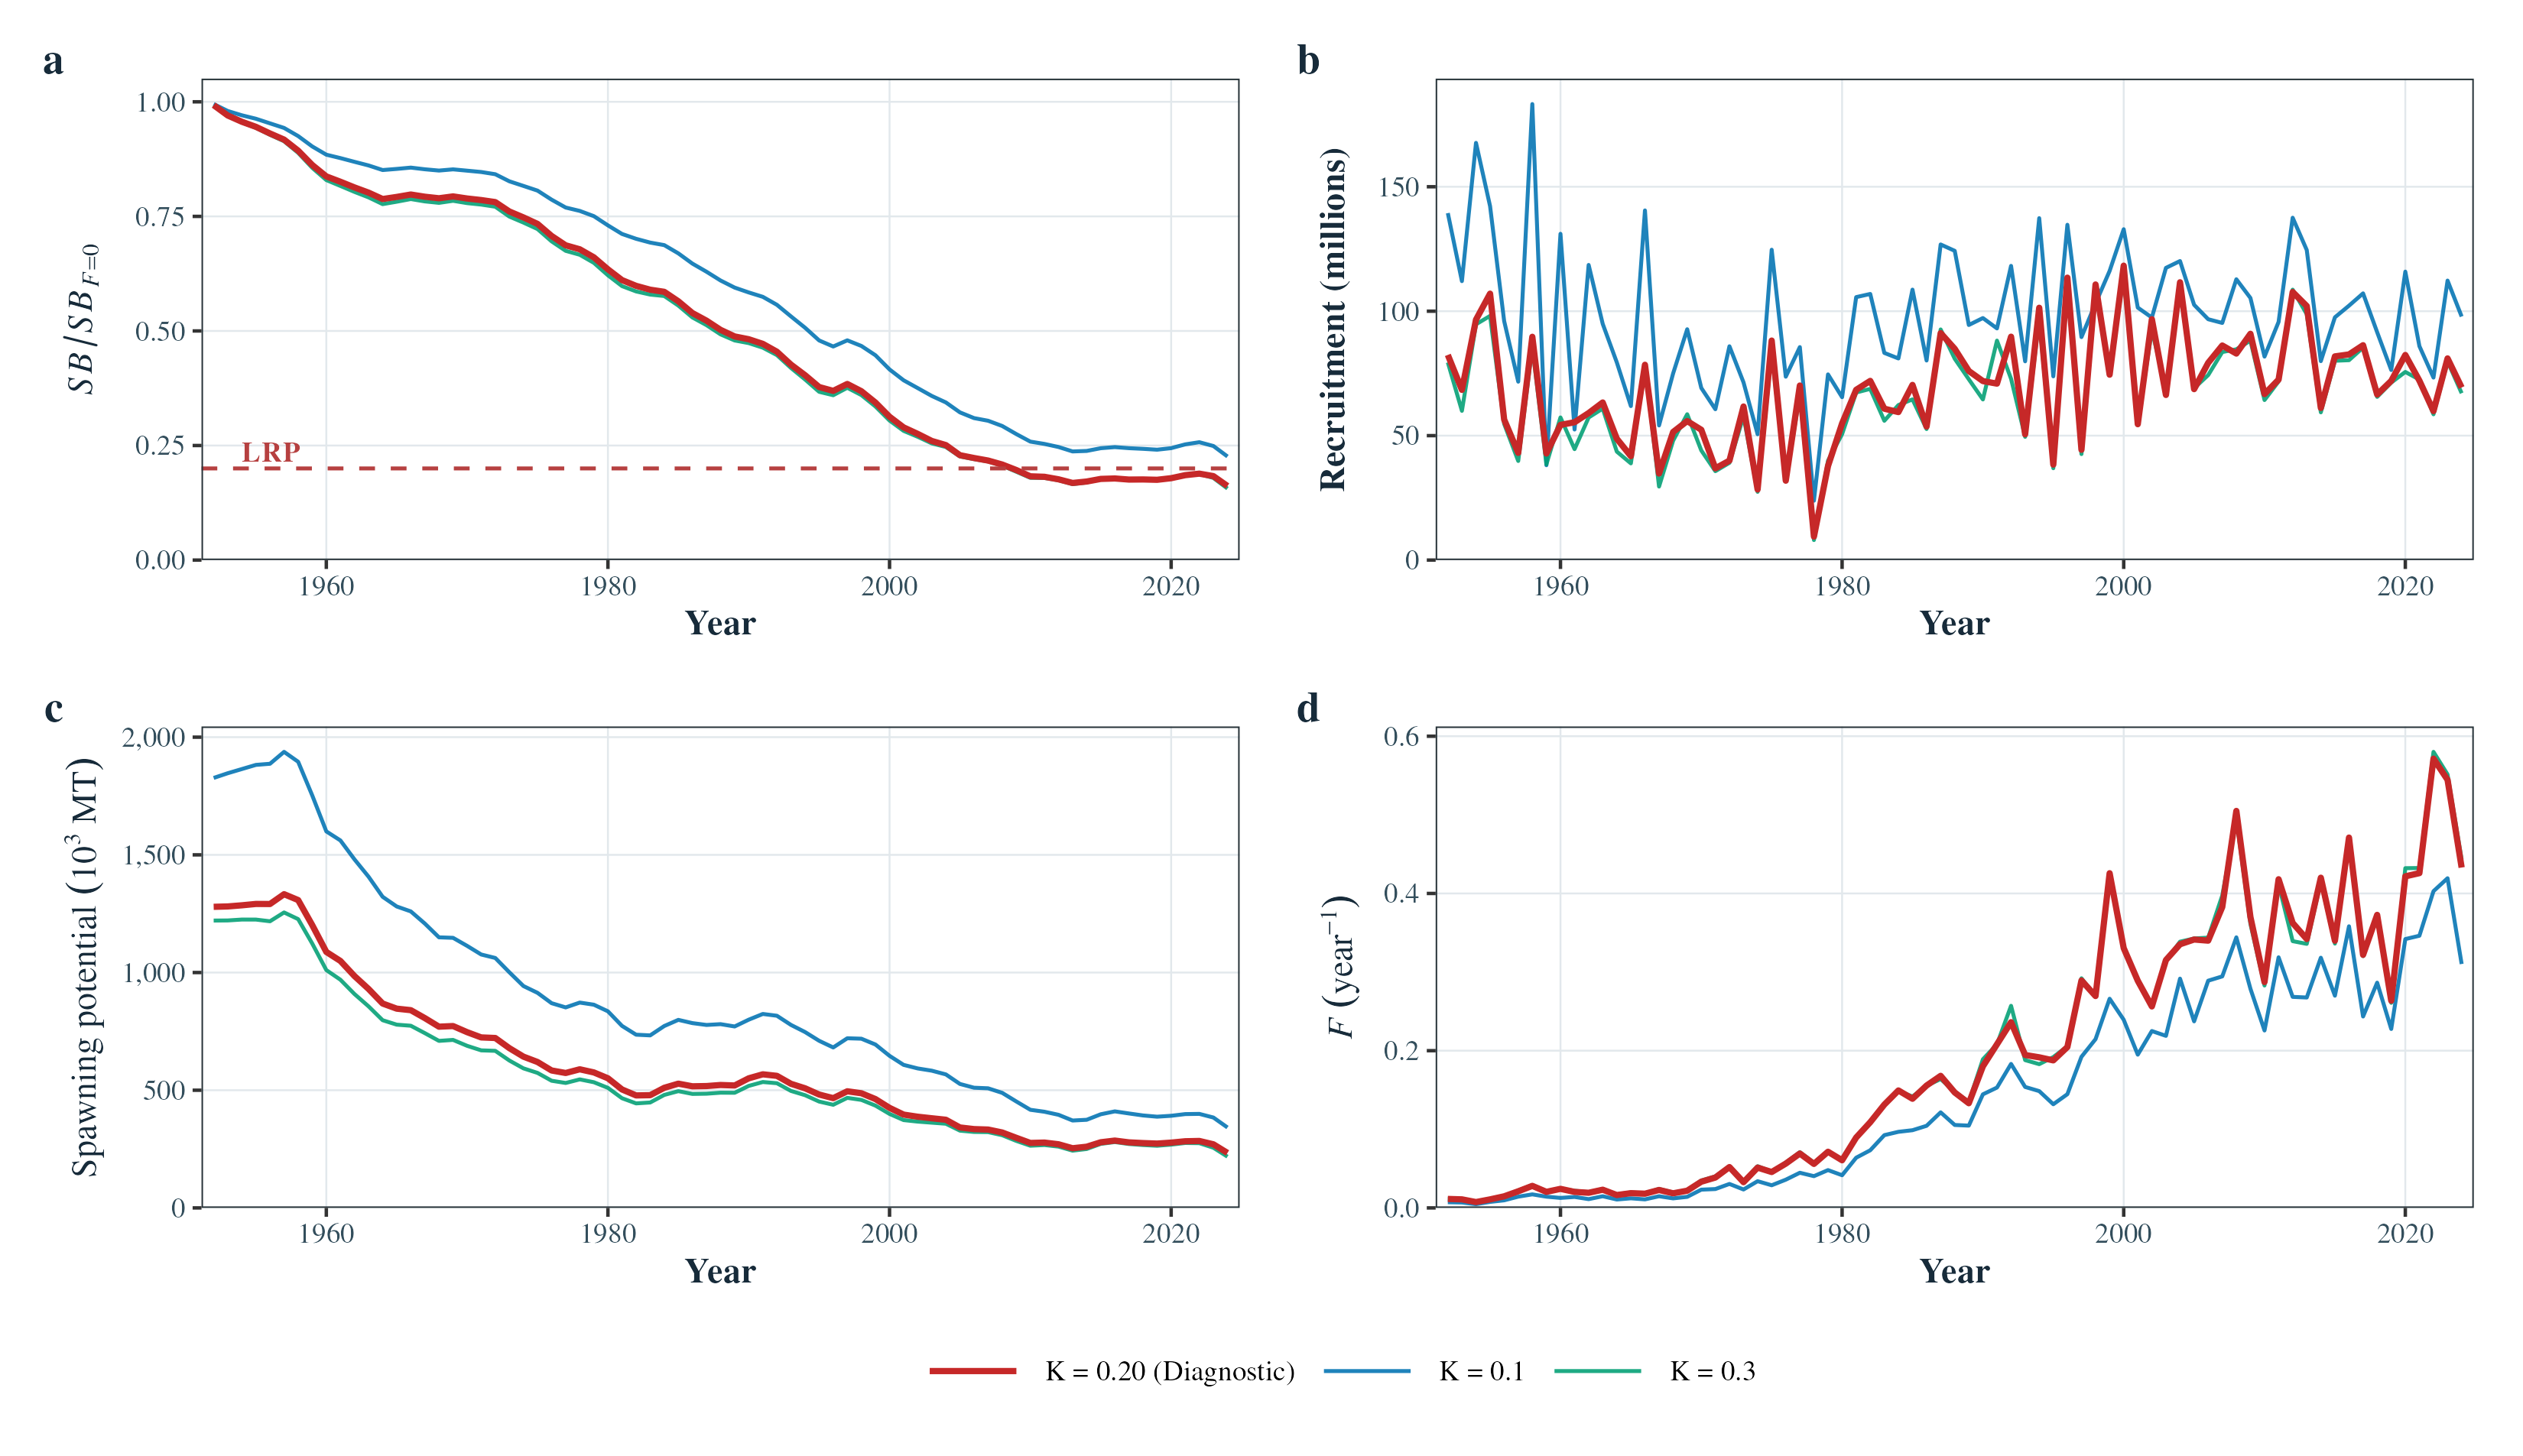
\includegraphics[width=1\linewidth,height=\textheight,keepaspectratio]{figures/sensitivity_tag_mixing_periods_Kstatistic_cutoff.png}

}

\caption{\label{fig-sensitivity-tag-mixing-periods-Kstatistic-cutoff}Estimated
dynamic spawning depletion (Top left) and spawning potential (Bottom
left), recruitment (Top right) and fishing mortality (Bottom right) for
the one-off sensitivities from the 2026 diagnostic model on the
K-statistic for assigning release group specific mixing periods - higher
value assume less conservative shorter mixing periods, lower value
assume more conservative longer mixing periods. Open the
\href{https://pacificcommunity.github.io/ofp-sam-bet-2026-sensitivity/bet-2026-sensitivity-interactive-viewer.html}{interactive
sensitivity viewer}.}

\end{figure}\DIFaddend %

\DIFdelbegin %DIFDELCMD < \begin{figure}[H]
%DIFDELCMD <

%DIFDELCMD < \centering{
%DIFDELCMD <

%DIFDELCMD < 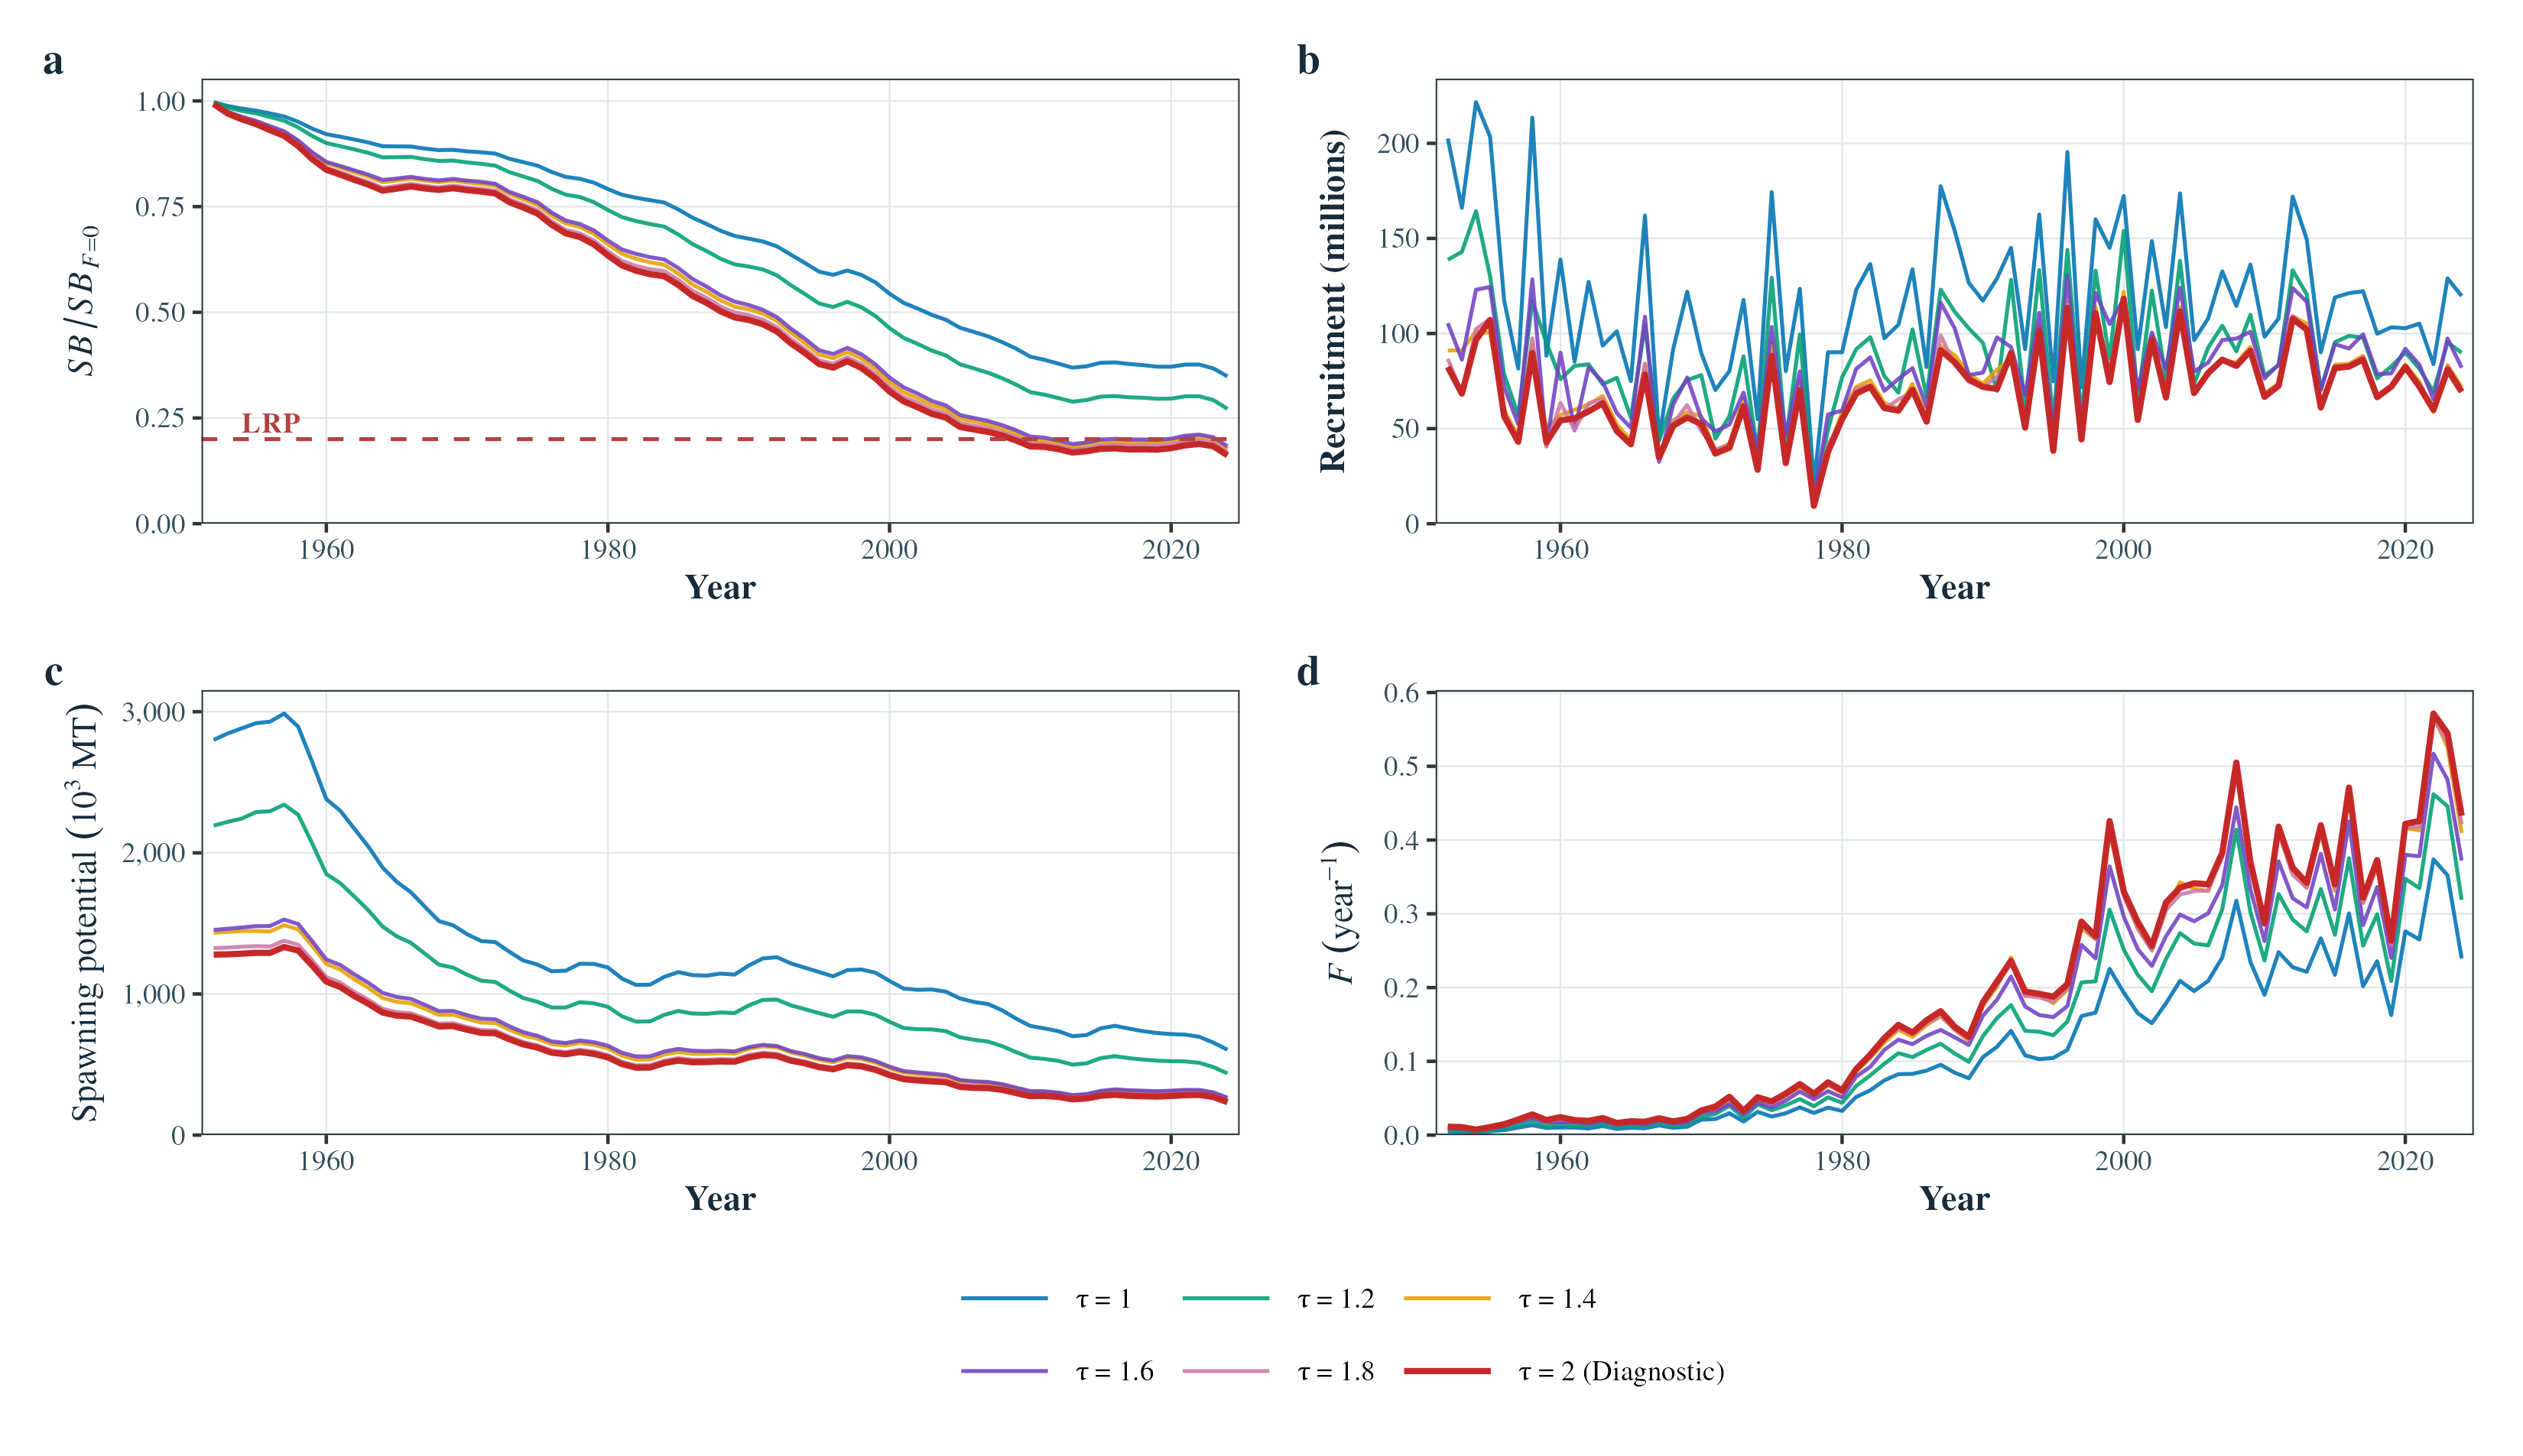
\includegraphics[width=1\linewidth,height=\textheight,keepaspectratio]{figures/sensitivity_tag_overdispersion.png}
%DIFDELCMD <

%DIFDELCMD < }
%DIFDELCMD <

%DIFDELCMD < \caption{\label{fig-sensitivity-tag-overdispersion}Estimated dynamic
%DIFDELCMD < spawning depletion (Top left) and spawning potential (Bottom left),
%DIFDELCMD < recruitment (Top right) and fishing mortality (Bottom right) for the
%DIFDELCMD < one-off sensitivities from the 2026 diagnostic model on assuming
%DIFDELCMD < different levels of the overdispersion parameter tau \(\tau\). Lower
%DIFDELCMD < values assume lower overdispersion and higher value higher over
%DIFDELCMD < dispersion.}
%DIFDELCMD <

%DIFDELCMD < \end{figure}%%%
\DIFdelend \DIFaddbegin \begin{figure}[H]

\centering{

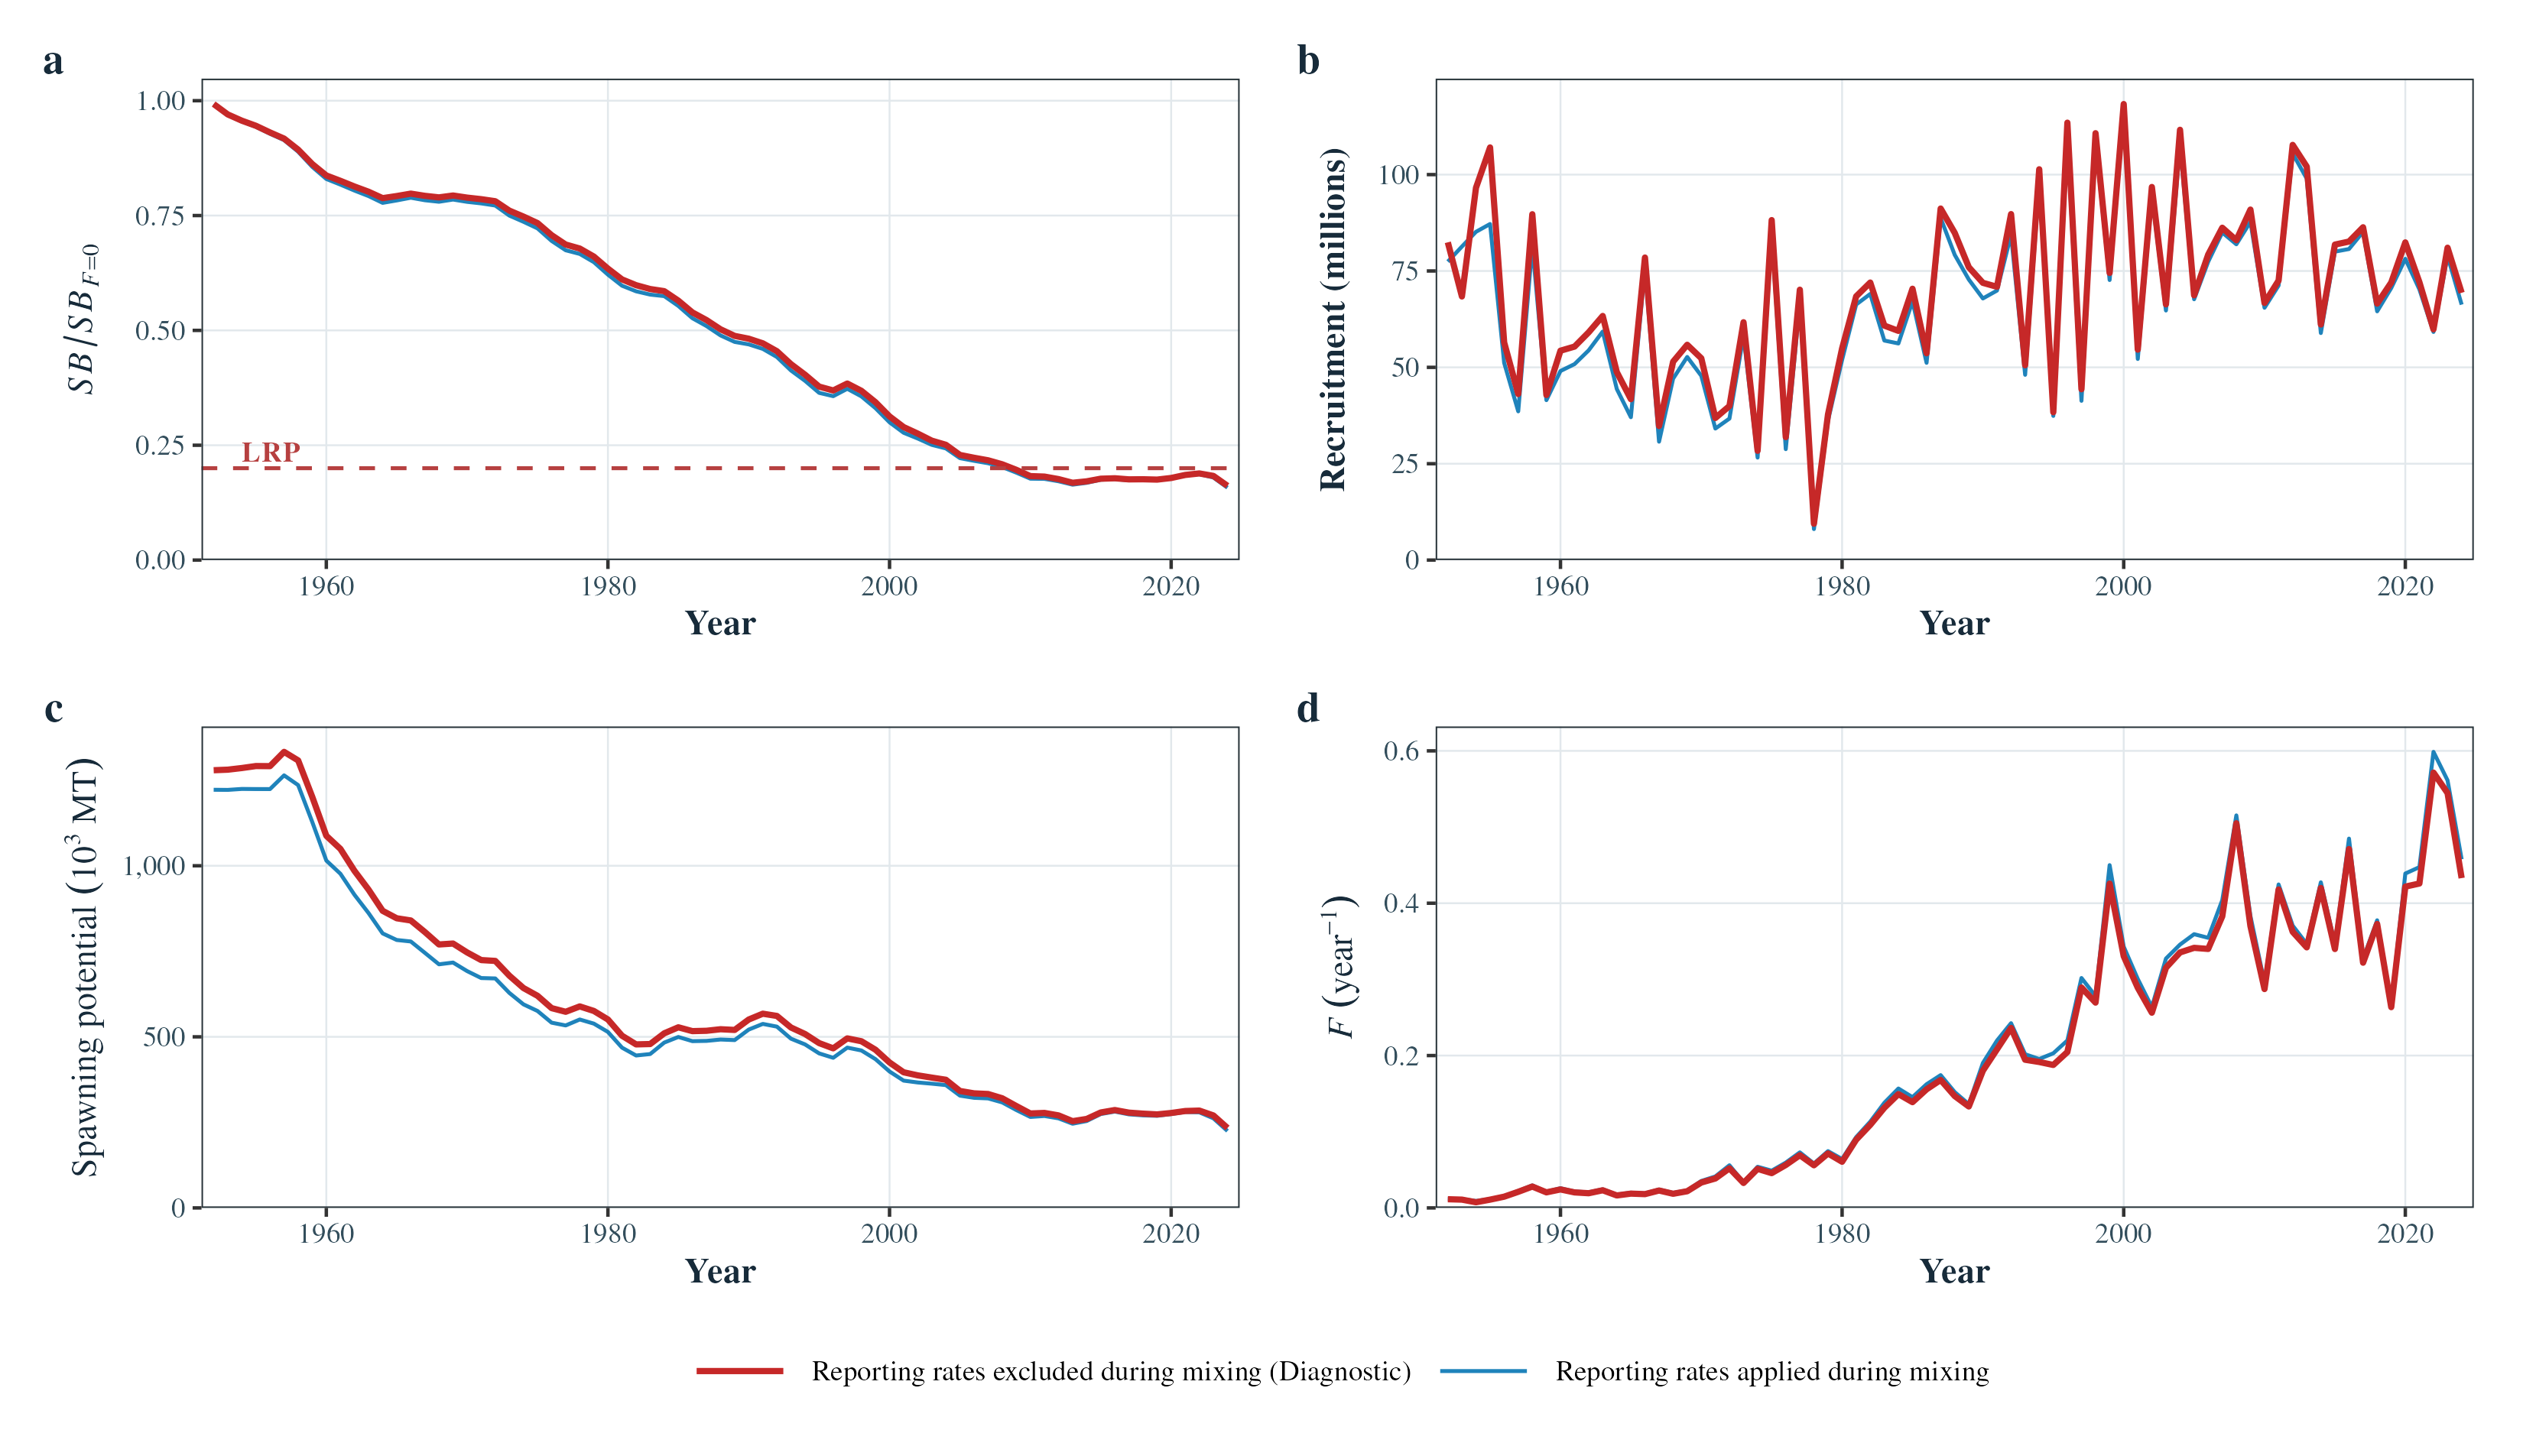
\includegraphics[width=1\linewidth,height=\textheight,keepaspectratio]{figures/sensitivity_premixing_tag_reporting_rate.png}

}

\caption{\label{fig-sensitivity-premixing-tag-reporting-rate}Estimated
dynamic spawning depletion (Top left) and spawning potential (Bottom
left), recruitment (Top right) and fishing mortality (Bottom right) for
the one-off sensitivities from the 2026 diagnostic model on the option
to activate or deactivate reporting rate adjustments during tag mixing
periods. Open the
\href{https://pacificcommunity.github.io/ofp-sam-bet-2026-sensitivity/bet-2026-sensitivity-interactive-viewer.html}{interactive
sensitivity viewer}.}

\end{figure}\DIFaddend %

\DIFdelbegin %DIFDELCMD < \begin{figure}[H]
%DIFDELCMD <

%DIFDELCMD < \centering{
%DIFDELCMD <

%DIFDELCMD < 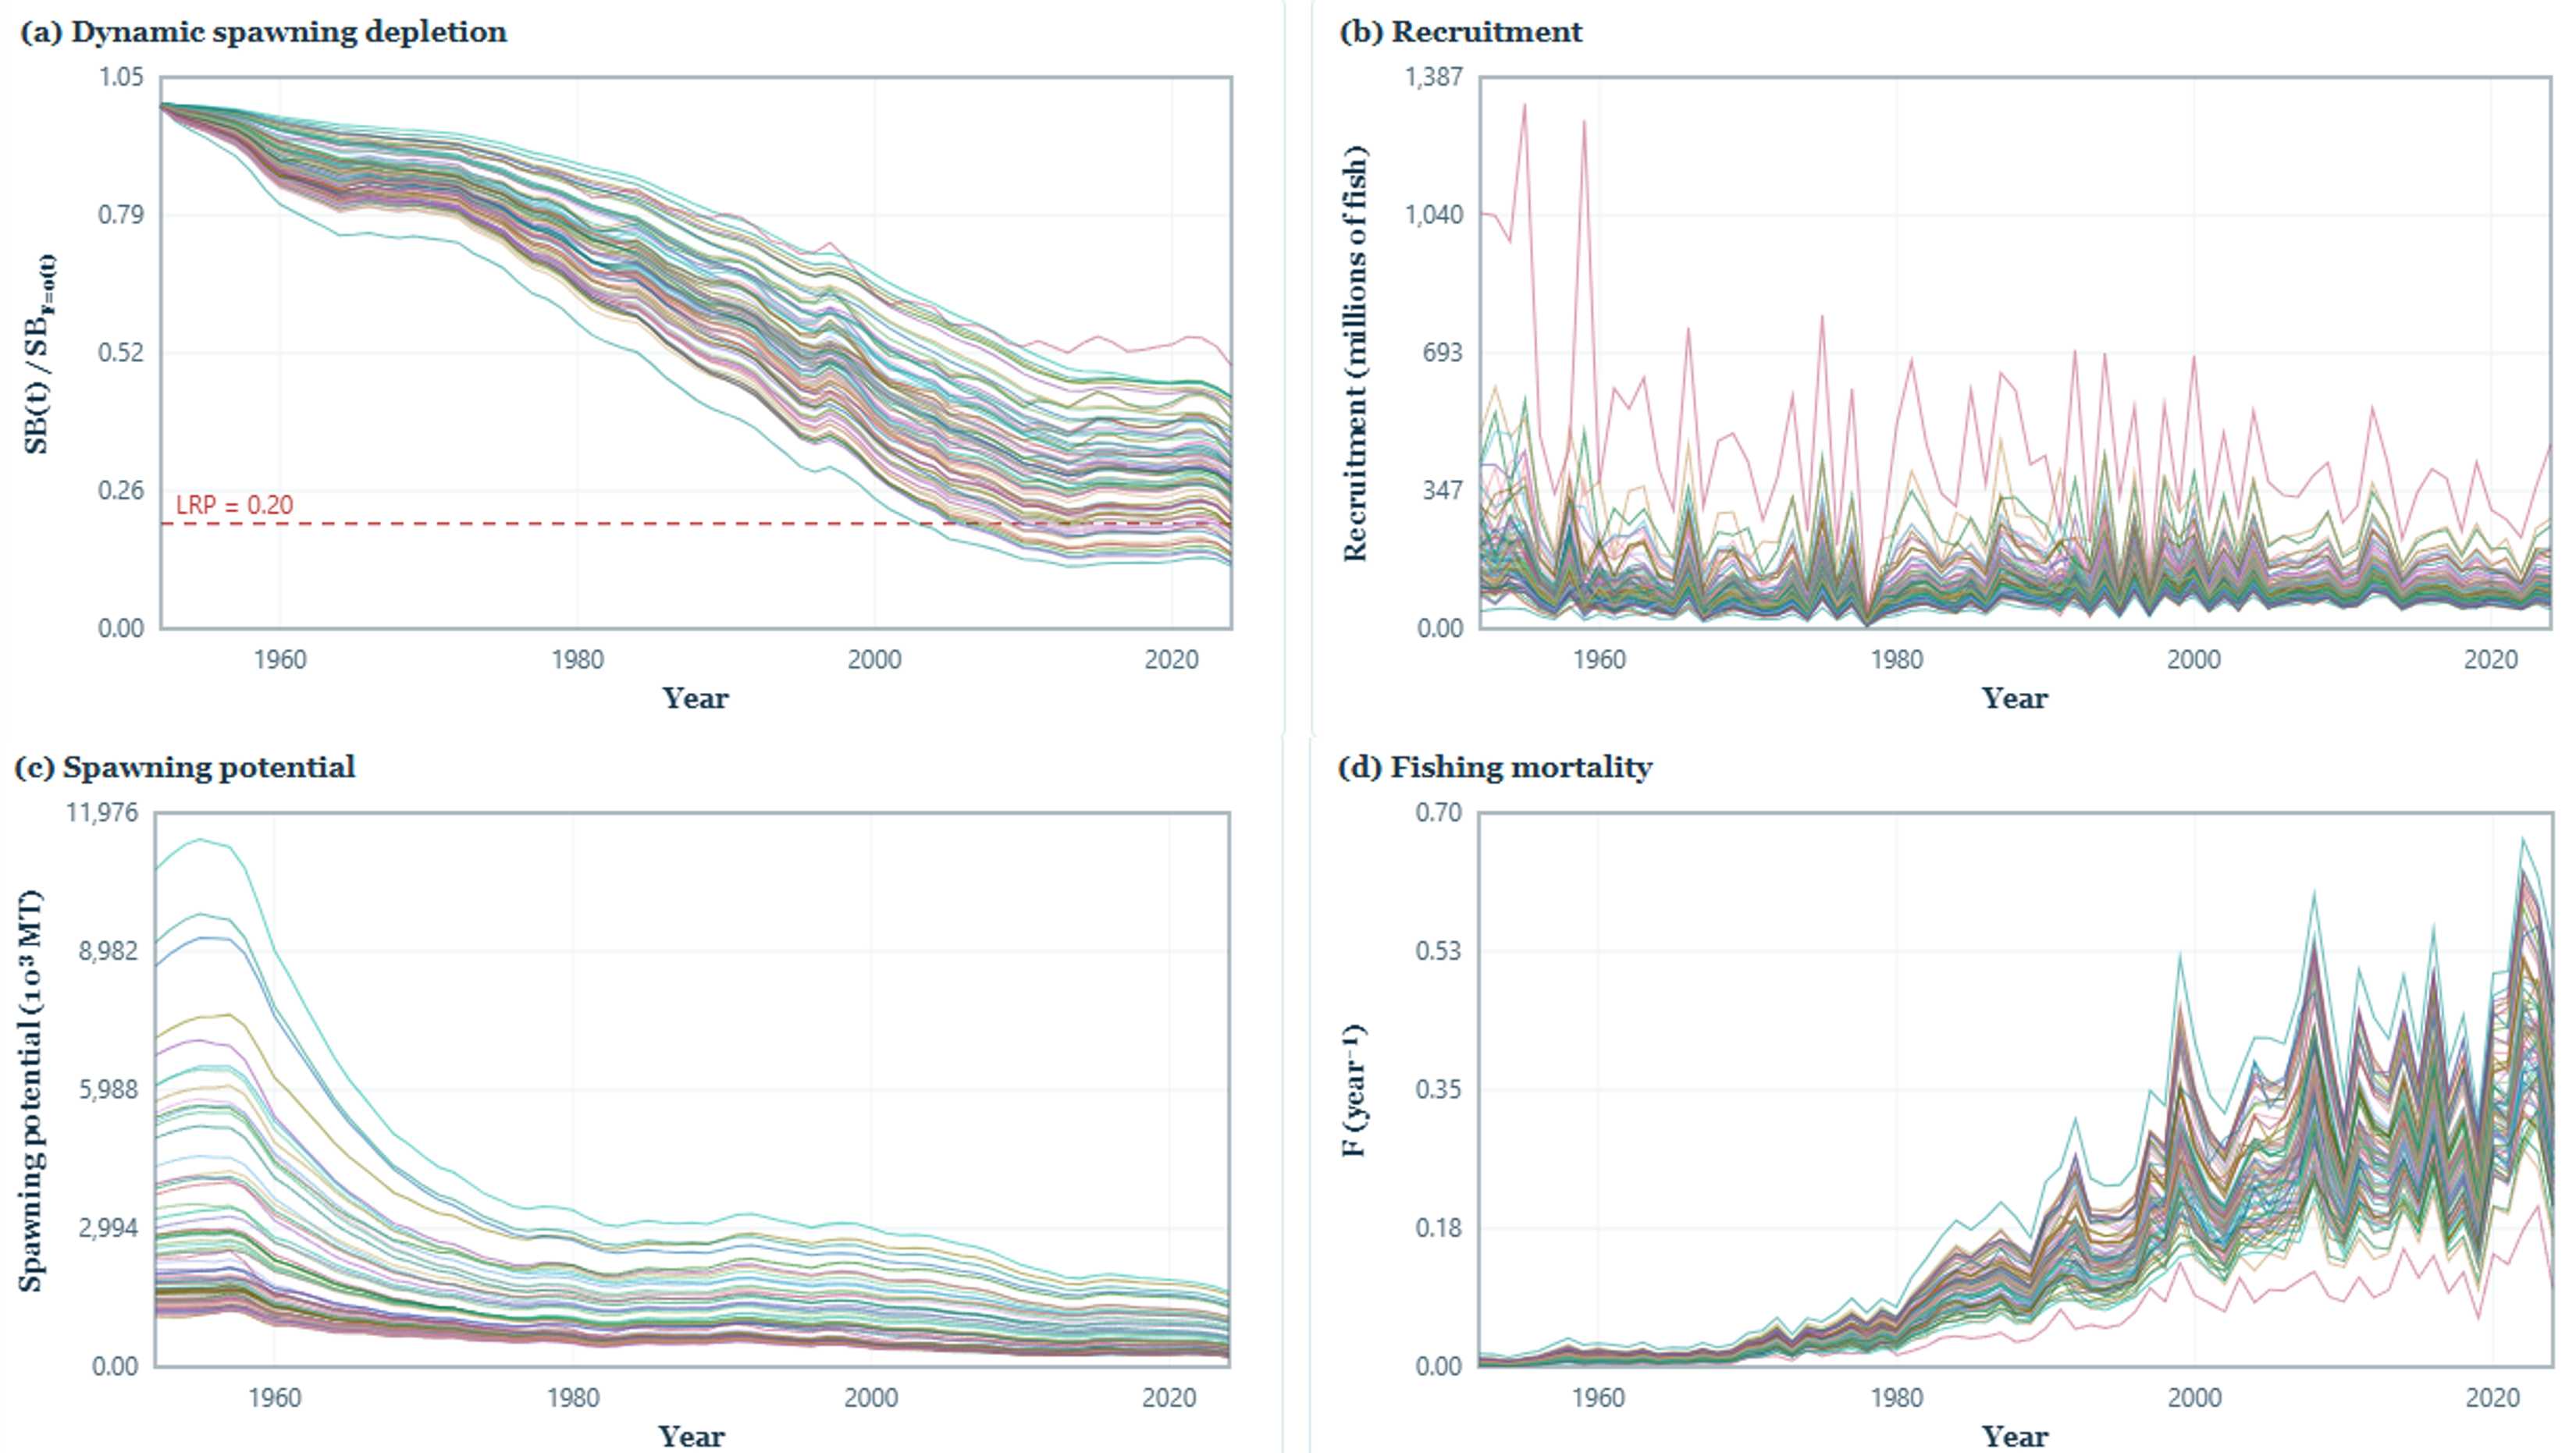
\includegraphics[width=1\linewidth,height=\textheight,keepaspectratio]{figures/ensemble_individual.png}
%DIFDELCMD <

%DIFDELCMD < }
%DIFDELCMD <

%DIFDELCMD < \caption{\label{fig-ensemble-individual}Estimated dynamic spawning
%DIFDELCMD < depletion (Top left) and spawning potential (Bottom left), recruitment
%DIFDELCMD < (Top right) and fishing mortality (Bottom right) for the 80 individual
%DIFDELCMD < models retained for the uncertainty ensemble.}
%DIFDELCMD <

%DIFDELCMD < \end{figure}%%%
\DIFdelend \DIFaddbegin \begin{figure}[H]

\centering{

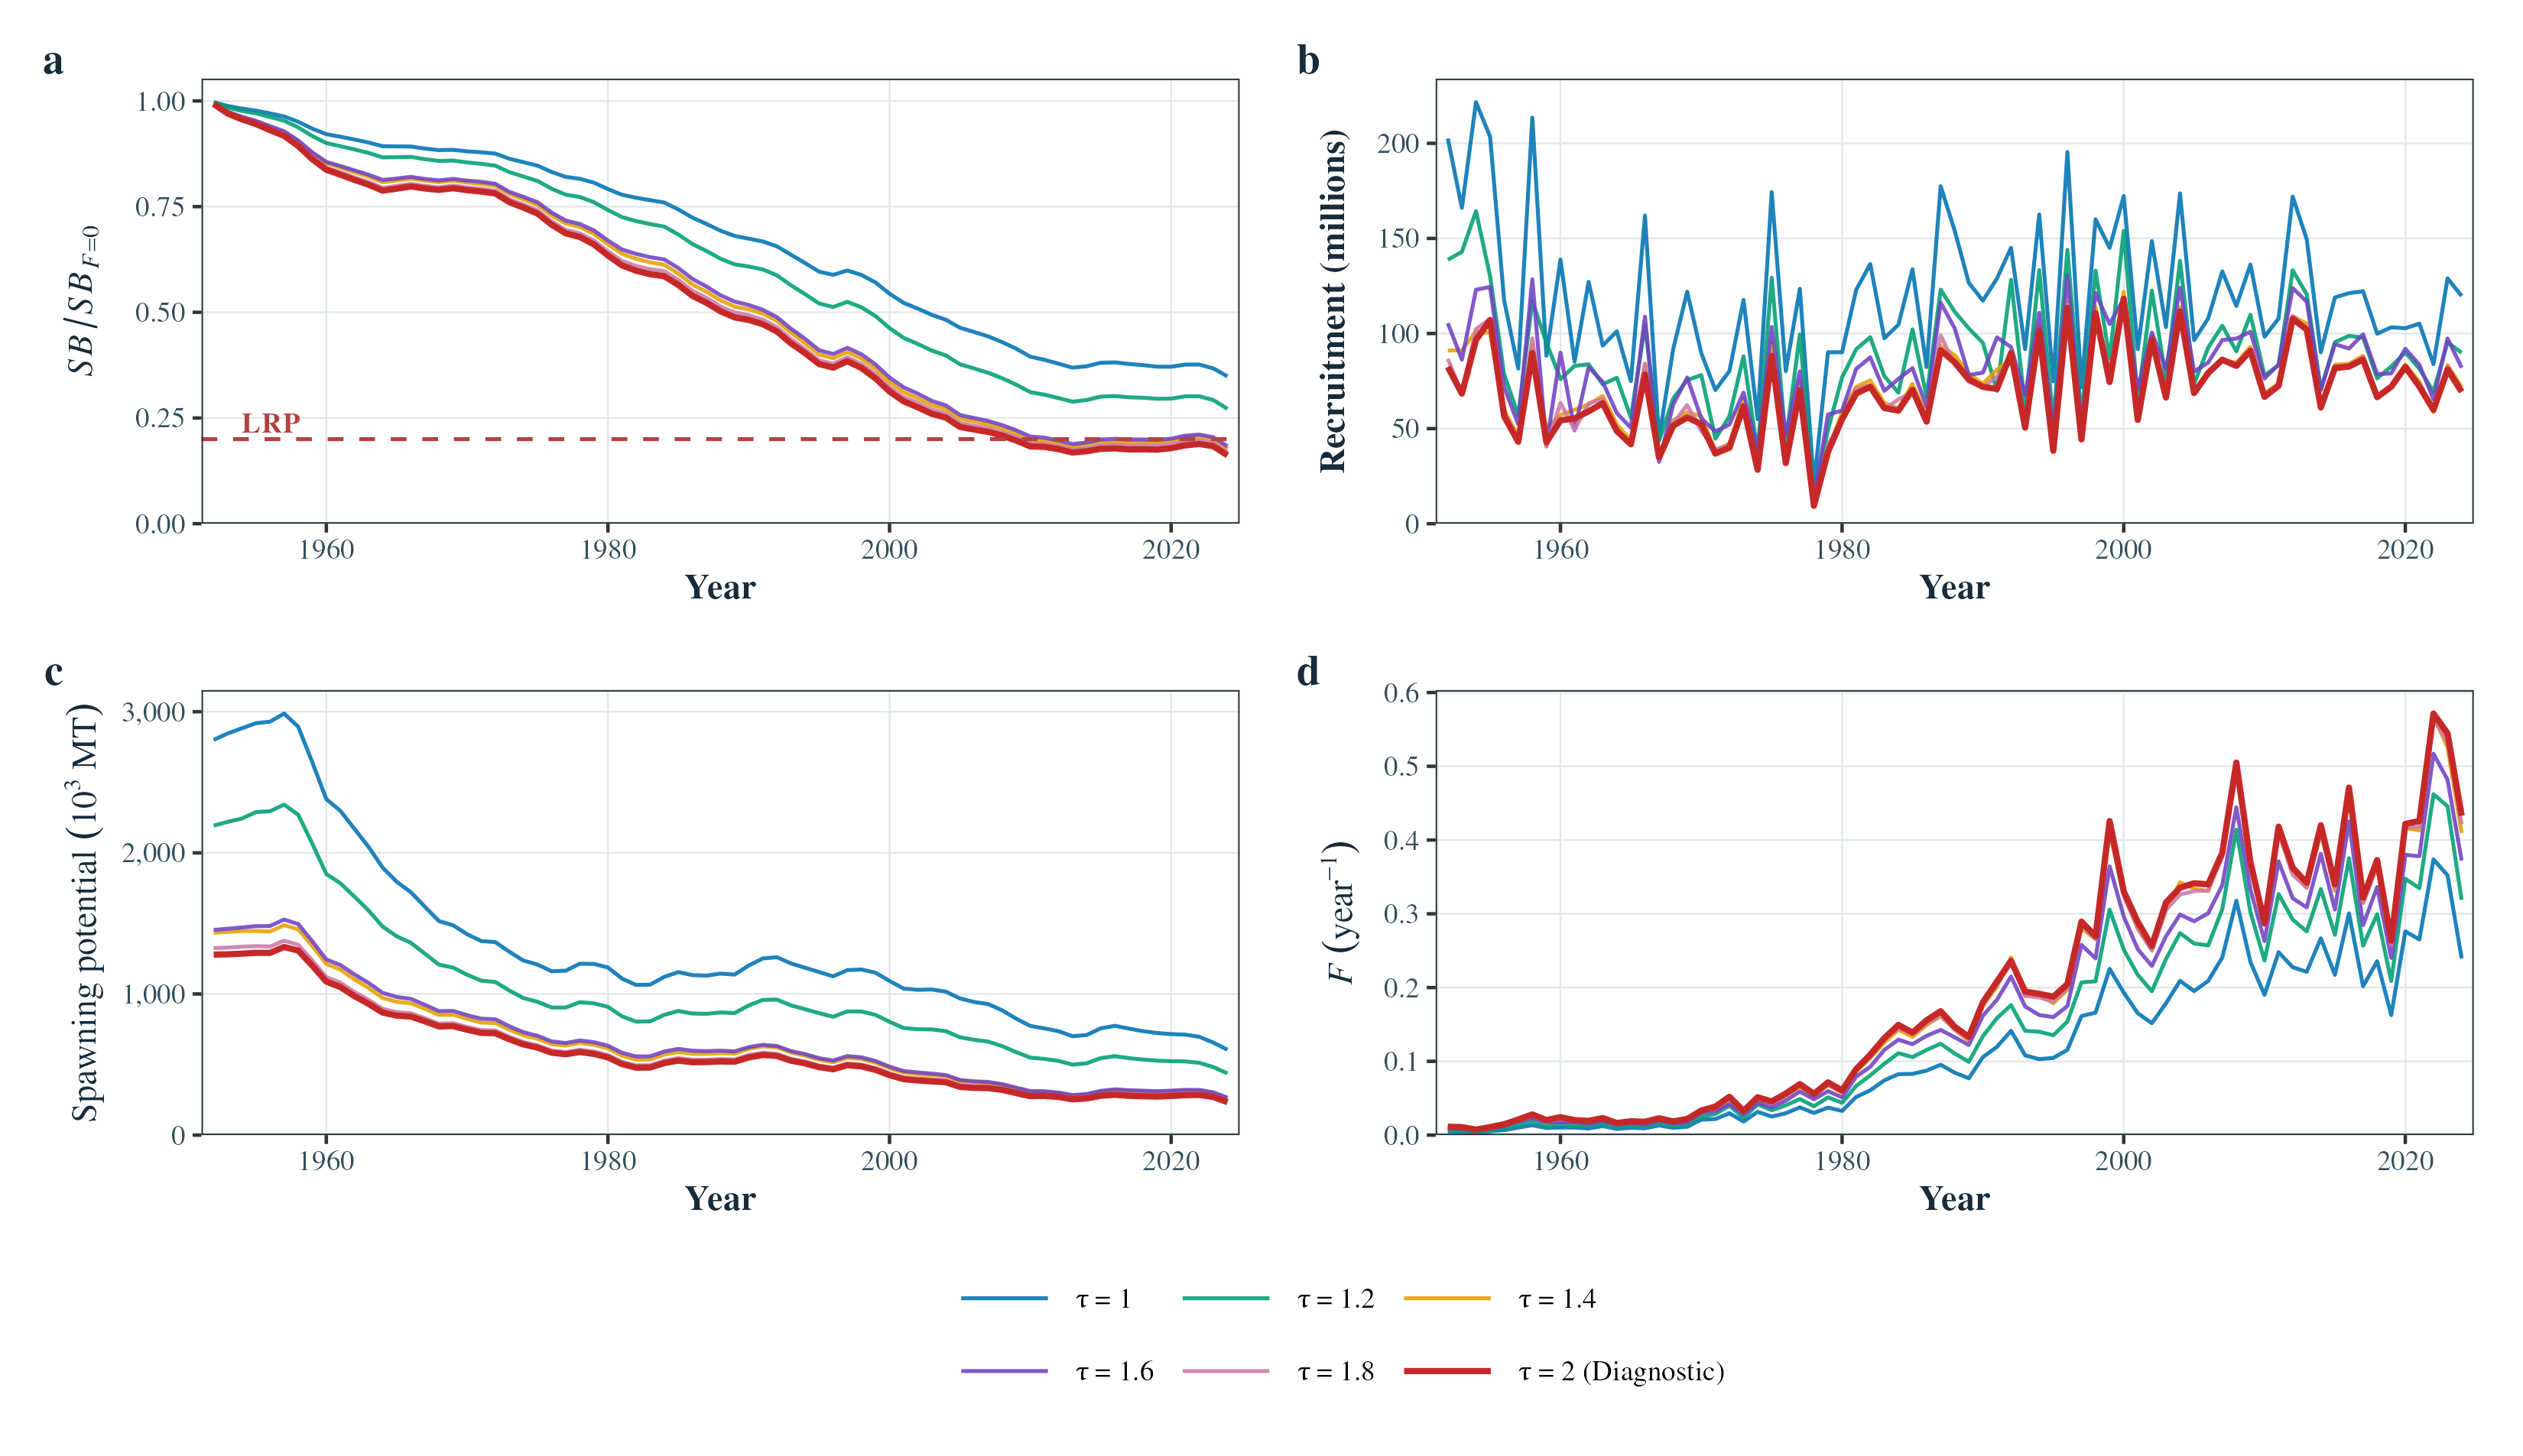
\includegraphics[width=1\linewidth,height=\textheight,keepaspectratio]{figures/sensitivity_tag_overdispersion.png}

}

\caption{\label{fig-sensitivity-tag-overdispersion}Dynamic spawning
depletion (top left), spawning potential (bottom left), recruitment (top
right) and fishing mortality (bottom right) for one-off sensitivities to
tag overdispersion \(\tau\). Lower values assign greater likelihood
weight to tag data; higher values allow greater extra-Poisson variation.
Open the
\href{https://pacificcommunity.github.io/ofp-sam-bet-2026-sensitivity/bet-2026-sensitivity-interactive-viewer.html}{interactive
sensitivity viewer}.}

\end{figure}\DIFaddend %

\DIFdelbegin %DIFDELCMD < \begin{figure}[H]
%DIFDELCMD <

%DIFDELCMD < \centering{
%DIFDELCMD <

%DIFDELCMD < 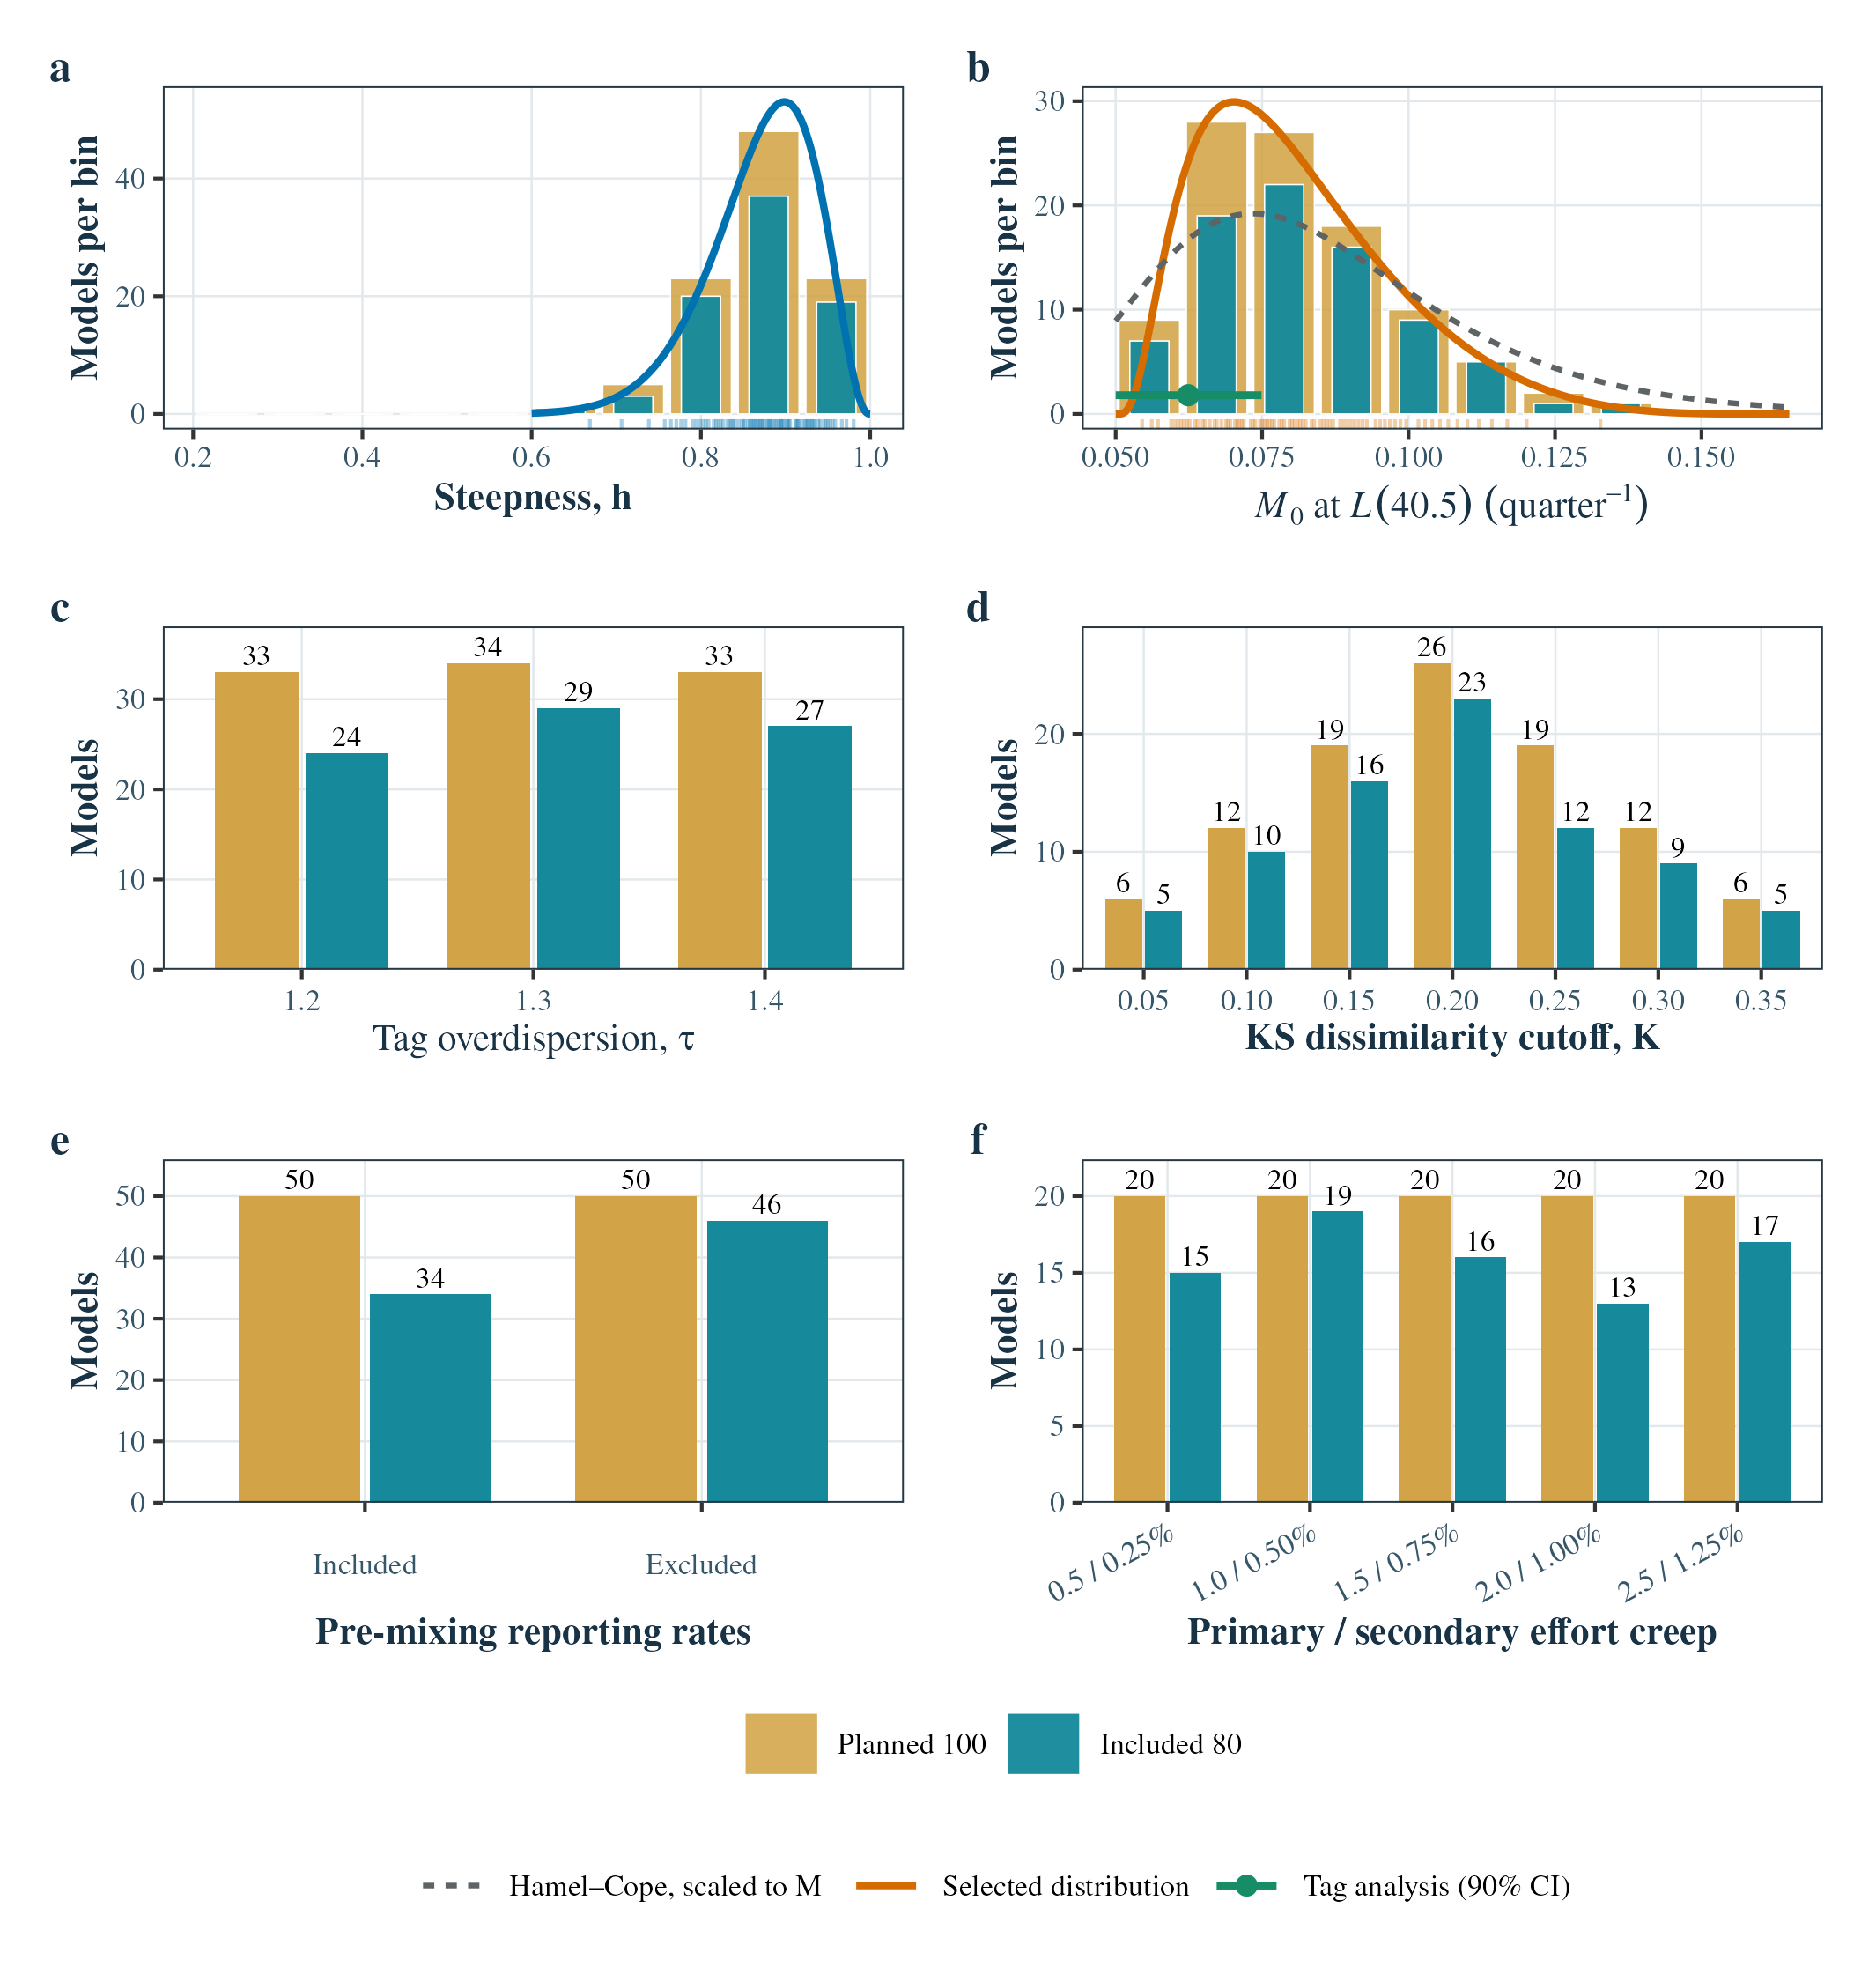
\includegraphics[width=1\linewidth,height=\textheight,keepaspectratio]{figures/ensemble_design_retention.png}
%DIFDELCMD <

%DIFDELCMD < }
%DIFDELCMD <

%DIFDELCMD < \caption{\label{fig-ensemble-design-retention}Planned and retained
%DIFDELCMD < ensemble model inputs: steepness (a), natural mortality at the reference
%DIFDELCMD < length (age 40 quarters) (b), tag overdispersion (c), tag-mixing cutoff
%DIFDELCMD < (d), pre-mixing reporting treatment (e), and effort creep (f). Gold
%DIFDELCMD < shows the 100 planned configurations and teal shows the 80 retained
%DIFDELCMD < models. Curves in panels a--b show the specified continuous input
%DIFDELCMD < distributions; the green point and line in panel b are the tag-based
%DIFDELCMD < estimate and 90\% confidence interval from Ducharme-Barth et al.
%DIFDELCMD < (2026).}
%DIFDELCMD <

%DIFDELCMD < \end{figure}%%%
\DIFdelend \DIFaddbegin \begin{figure}[H]

\centering{

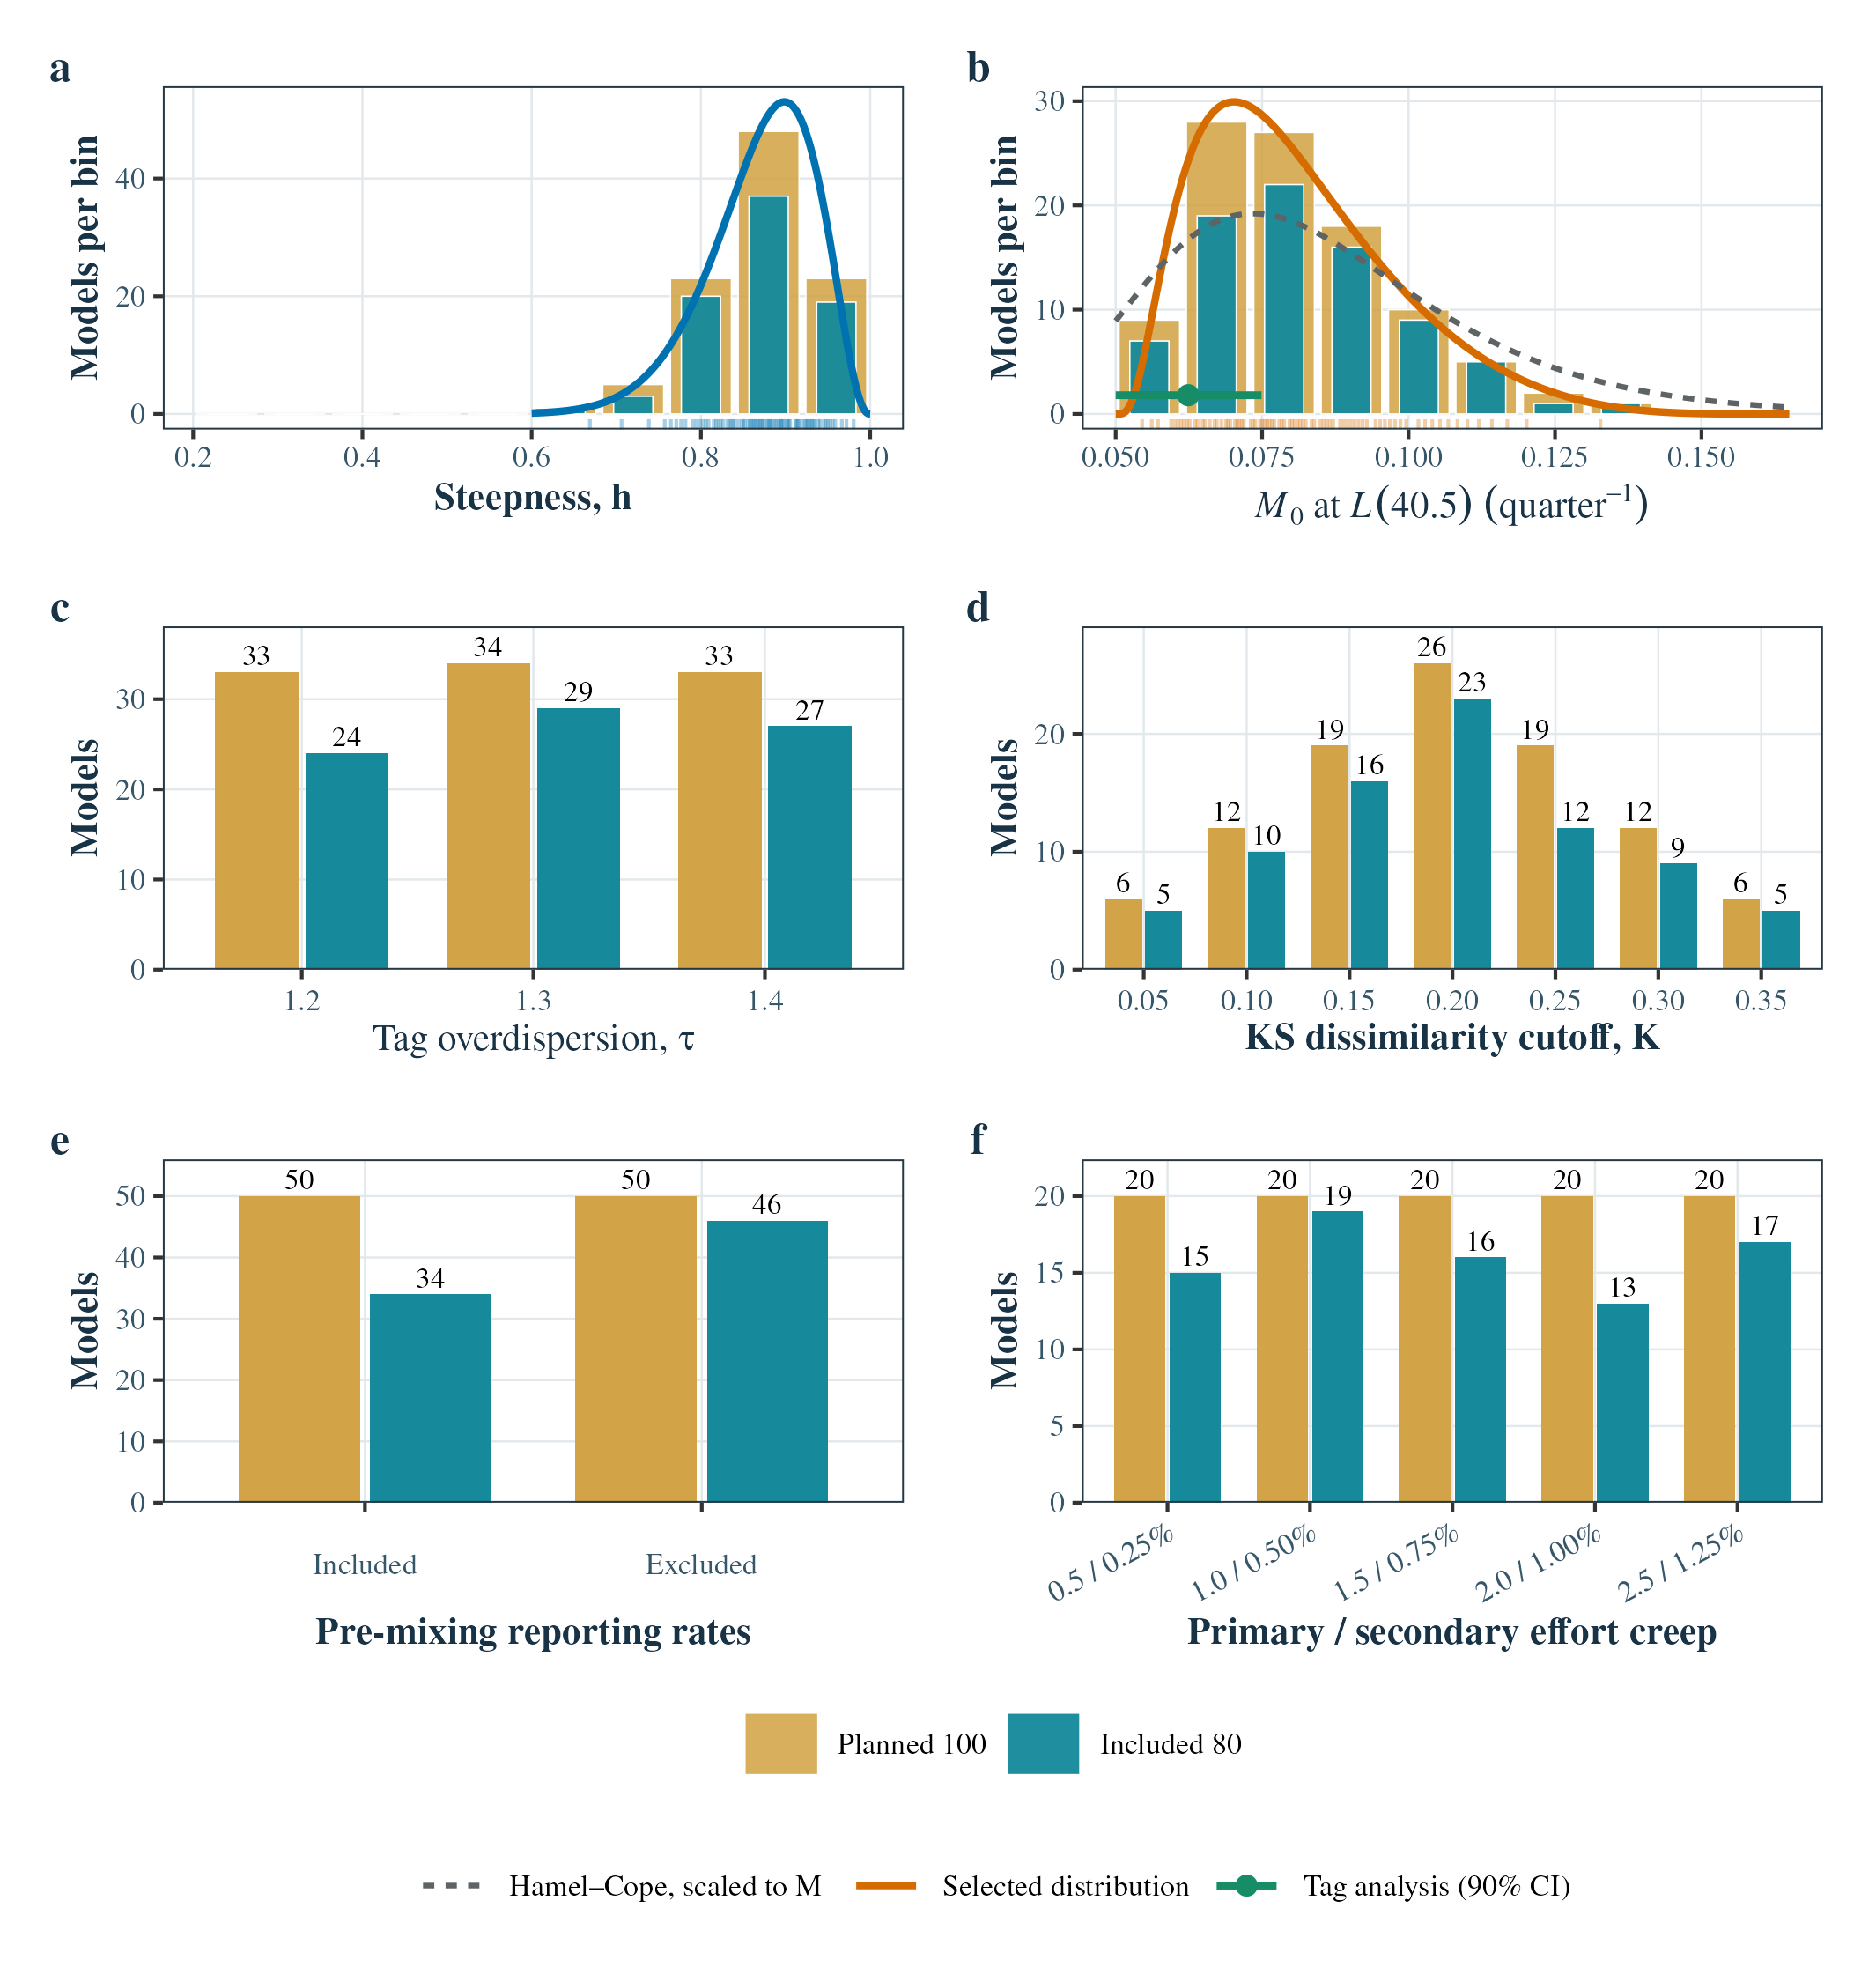
\includegraphics[width=1\linewidth,height=\textheight,keepaspectratio]{figures/ensemble_design_retention.png}

}

\caption{\label{fig-ensemble-design-retention}Planned and retained
ensemble model inputs: steepness (a), natural mortality at the reference
length (age 40 quarters) (b), tag overdispersion (c), tag-mixing cutoff
(d), pre-mixing reporting treatment (e), and effort creep (f). Gold
shows the 100 planned configurations and teal shows the 80 retained
models. Curves in panels a--b show the specified continuous input
distributions; the green point and line in panel b are the tag-based
estimate and 90\% confidence interval from Ducharme-Barth et al. (2026).
Open the
\href{https://pacificcommunity.github.io/ofp-sam-bet-2026-ensemble/bet-2026-ensemble-interactive-viewer.html}{interactive
ensemble viewer}.}

\end{figure}\DIFaddend %

\DIFdelbegin %DIFDELCMD < \begin{figure}[H]
%DIFDELCMD <

%DIFDELCMD < \centering{
%DIFDELCMD <

%DIFDELCMD < 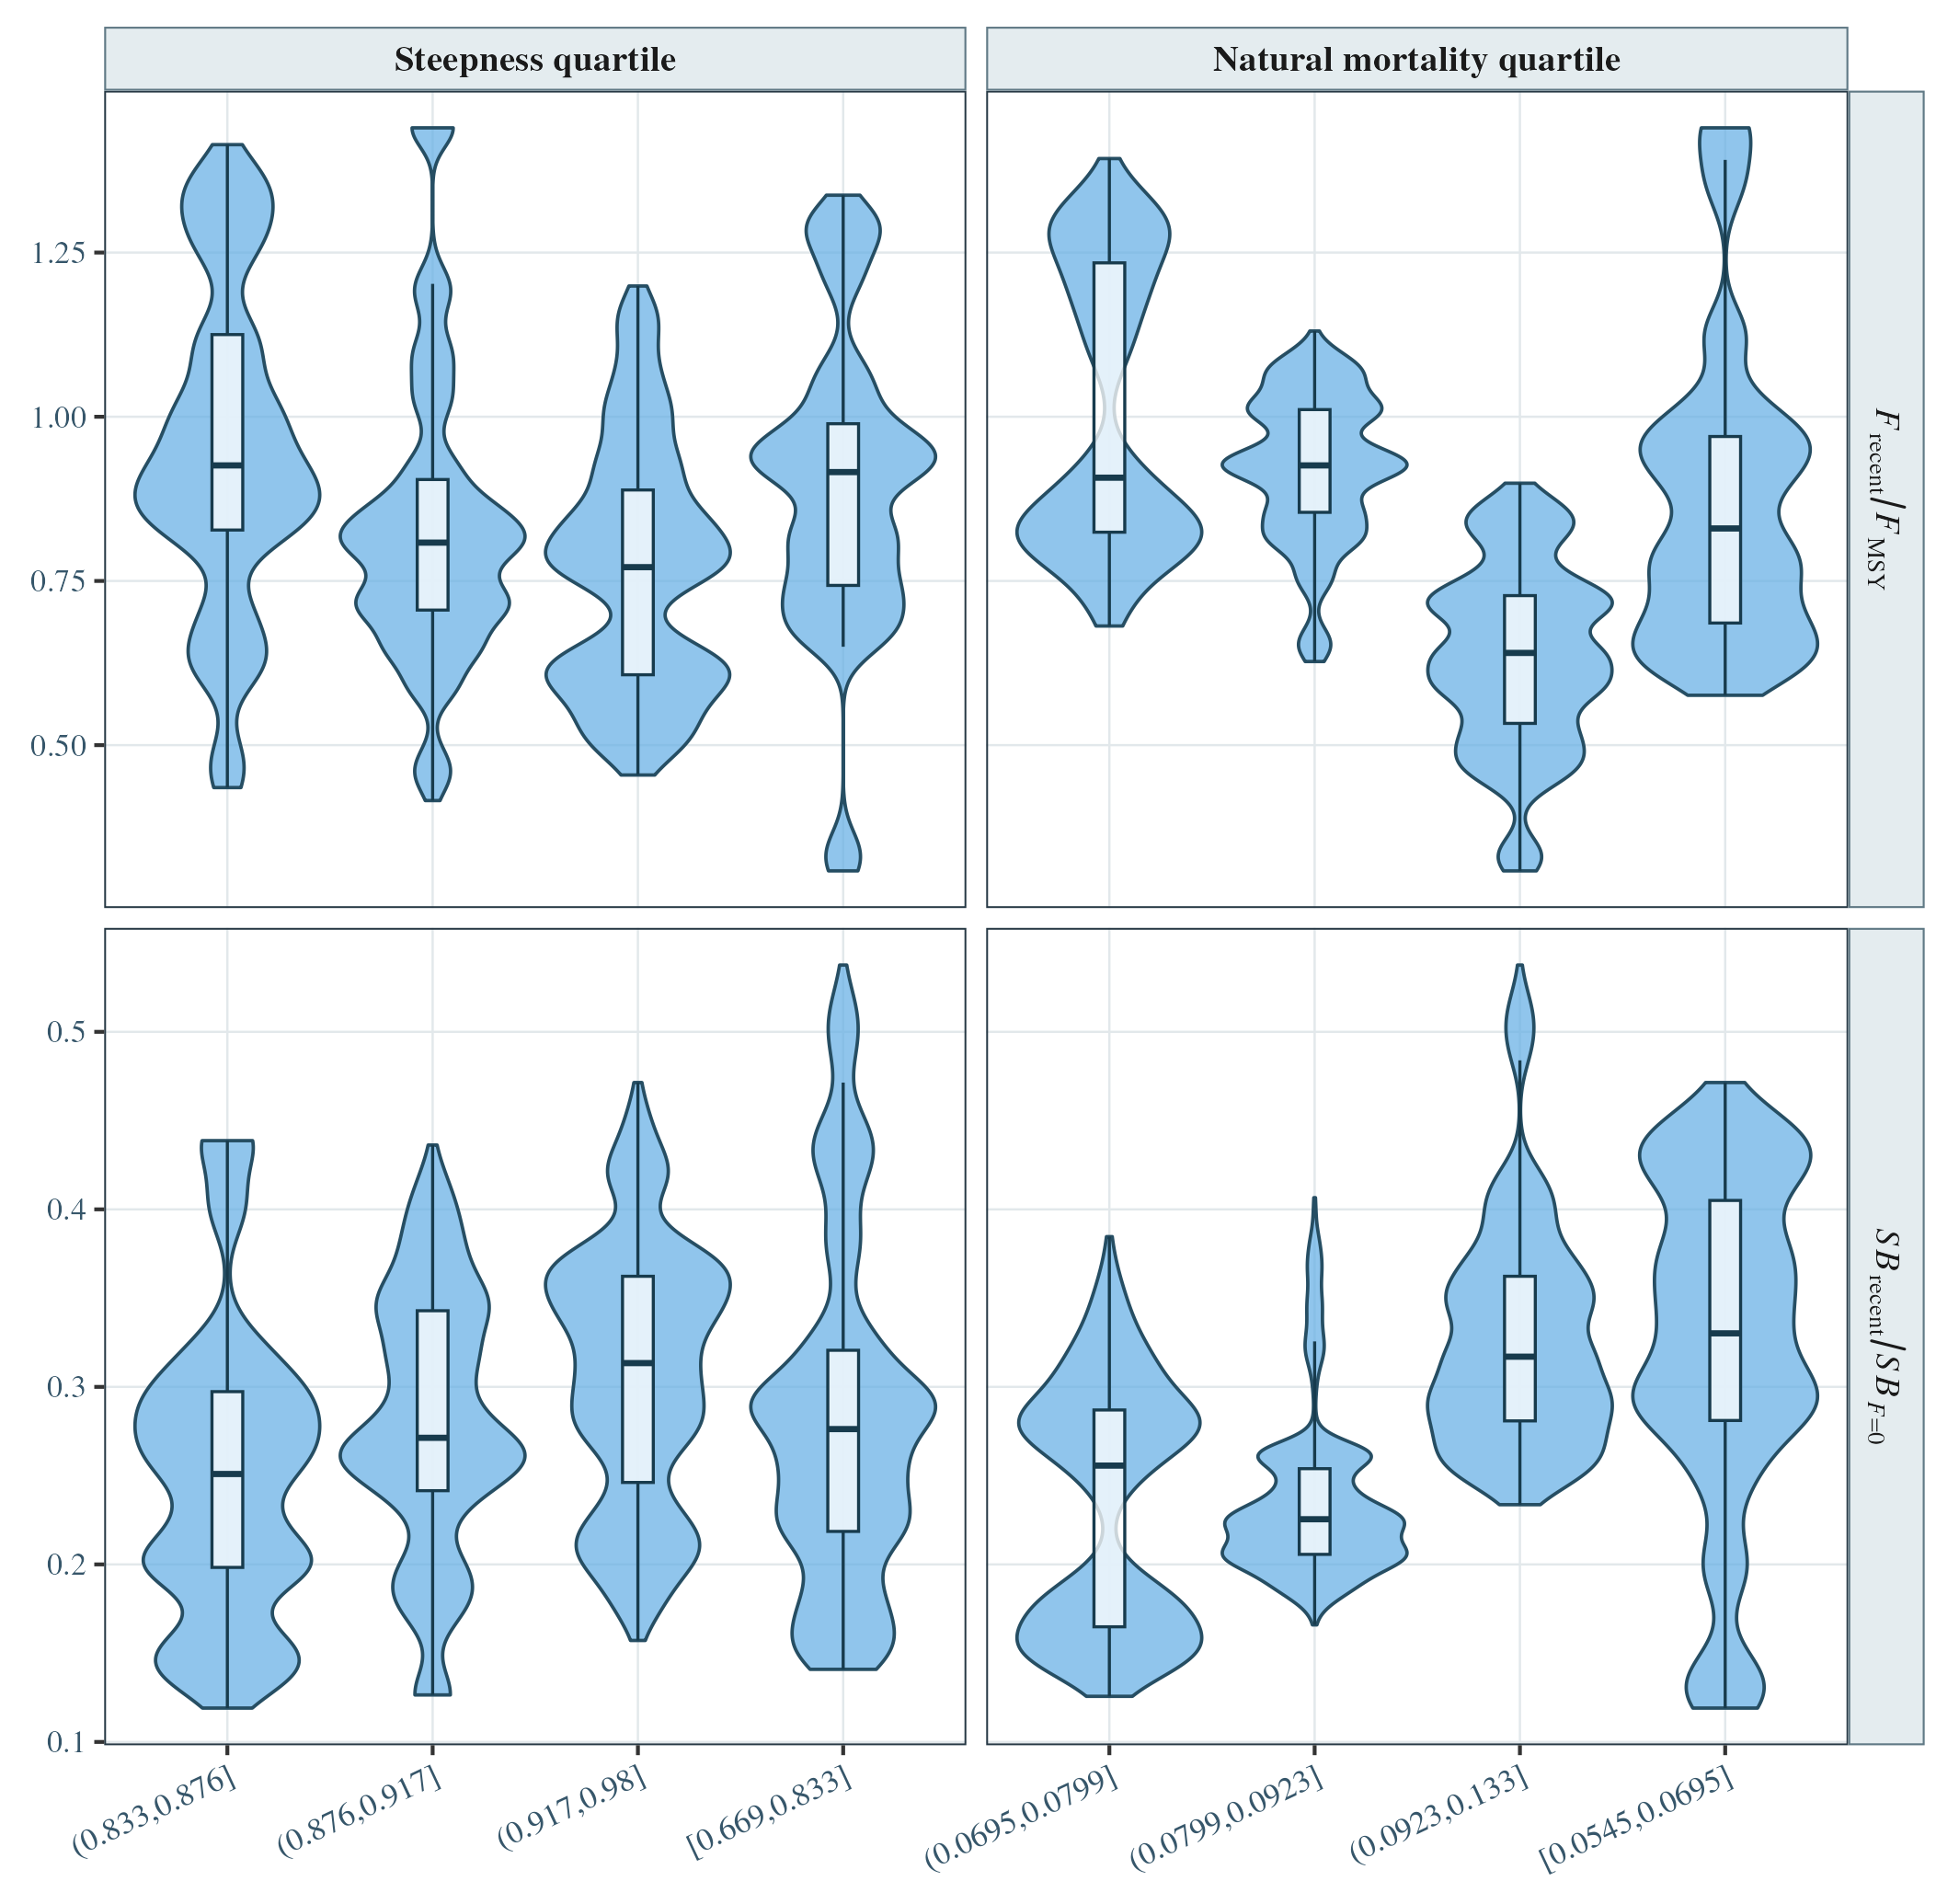
\includegraphics[width=1\linewidth,height=\textheight,keepaspectratio]{figures/management-uncertainty-continuous-axes_steep_M.png}
%DIFDELCMD <

%DIFDELCMD < }
%DIFDELCMD <

%DIFDELCMD < \caption{\label{fig-management-uncertainty-continuous-axes-steep-M}All-model
%DIFDELCMD < uncertainty distributions of \(F_{recent}\)/\(F_{MSY}\) (top) and
%DIFDELCMD < \(SB_{recent}\)/\(SB_{F=0}\) (bottom), grouped by quartiles of steepness
%DIFDELCMD < and natural mortality at the reference length. Violin width represents
%DIFDELCMD < density and the inset box shows the interquartile range and median. Each
%DIFDELCMD < model has equal total weight; PDH models contribute joint Hessian draws
%DIFDELCMD < and Near-PDH models contribute their central estimates. Because all
%DIFDELCMD < ensemble axes vary jointly, differences among groups are descriptive and
%DIFDELCMD < not one-factor causal effects.}
%DIFDELCMD <

%DIFDELCMD < \end{figure}%%%
\DIFdelend \DIFaddbegin \begin{figure}[H]

\centering{

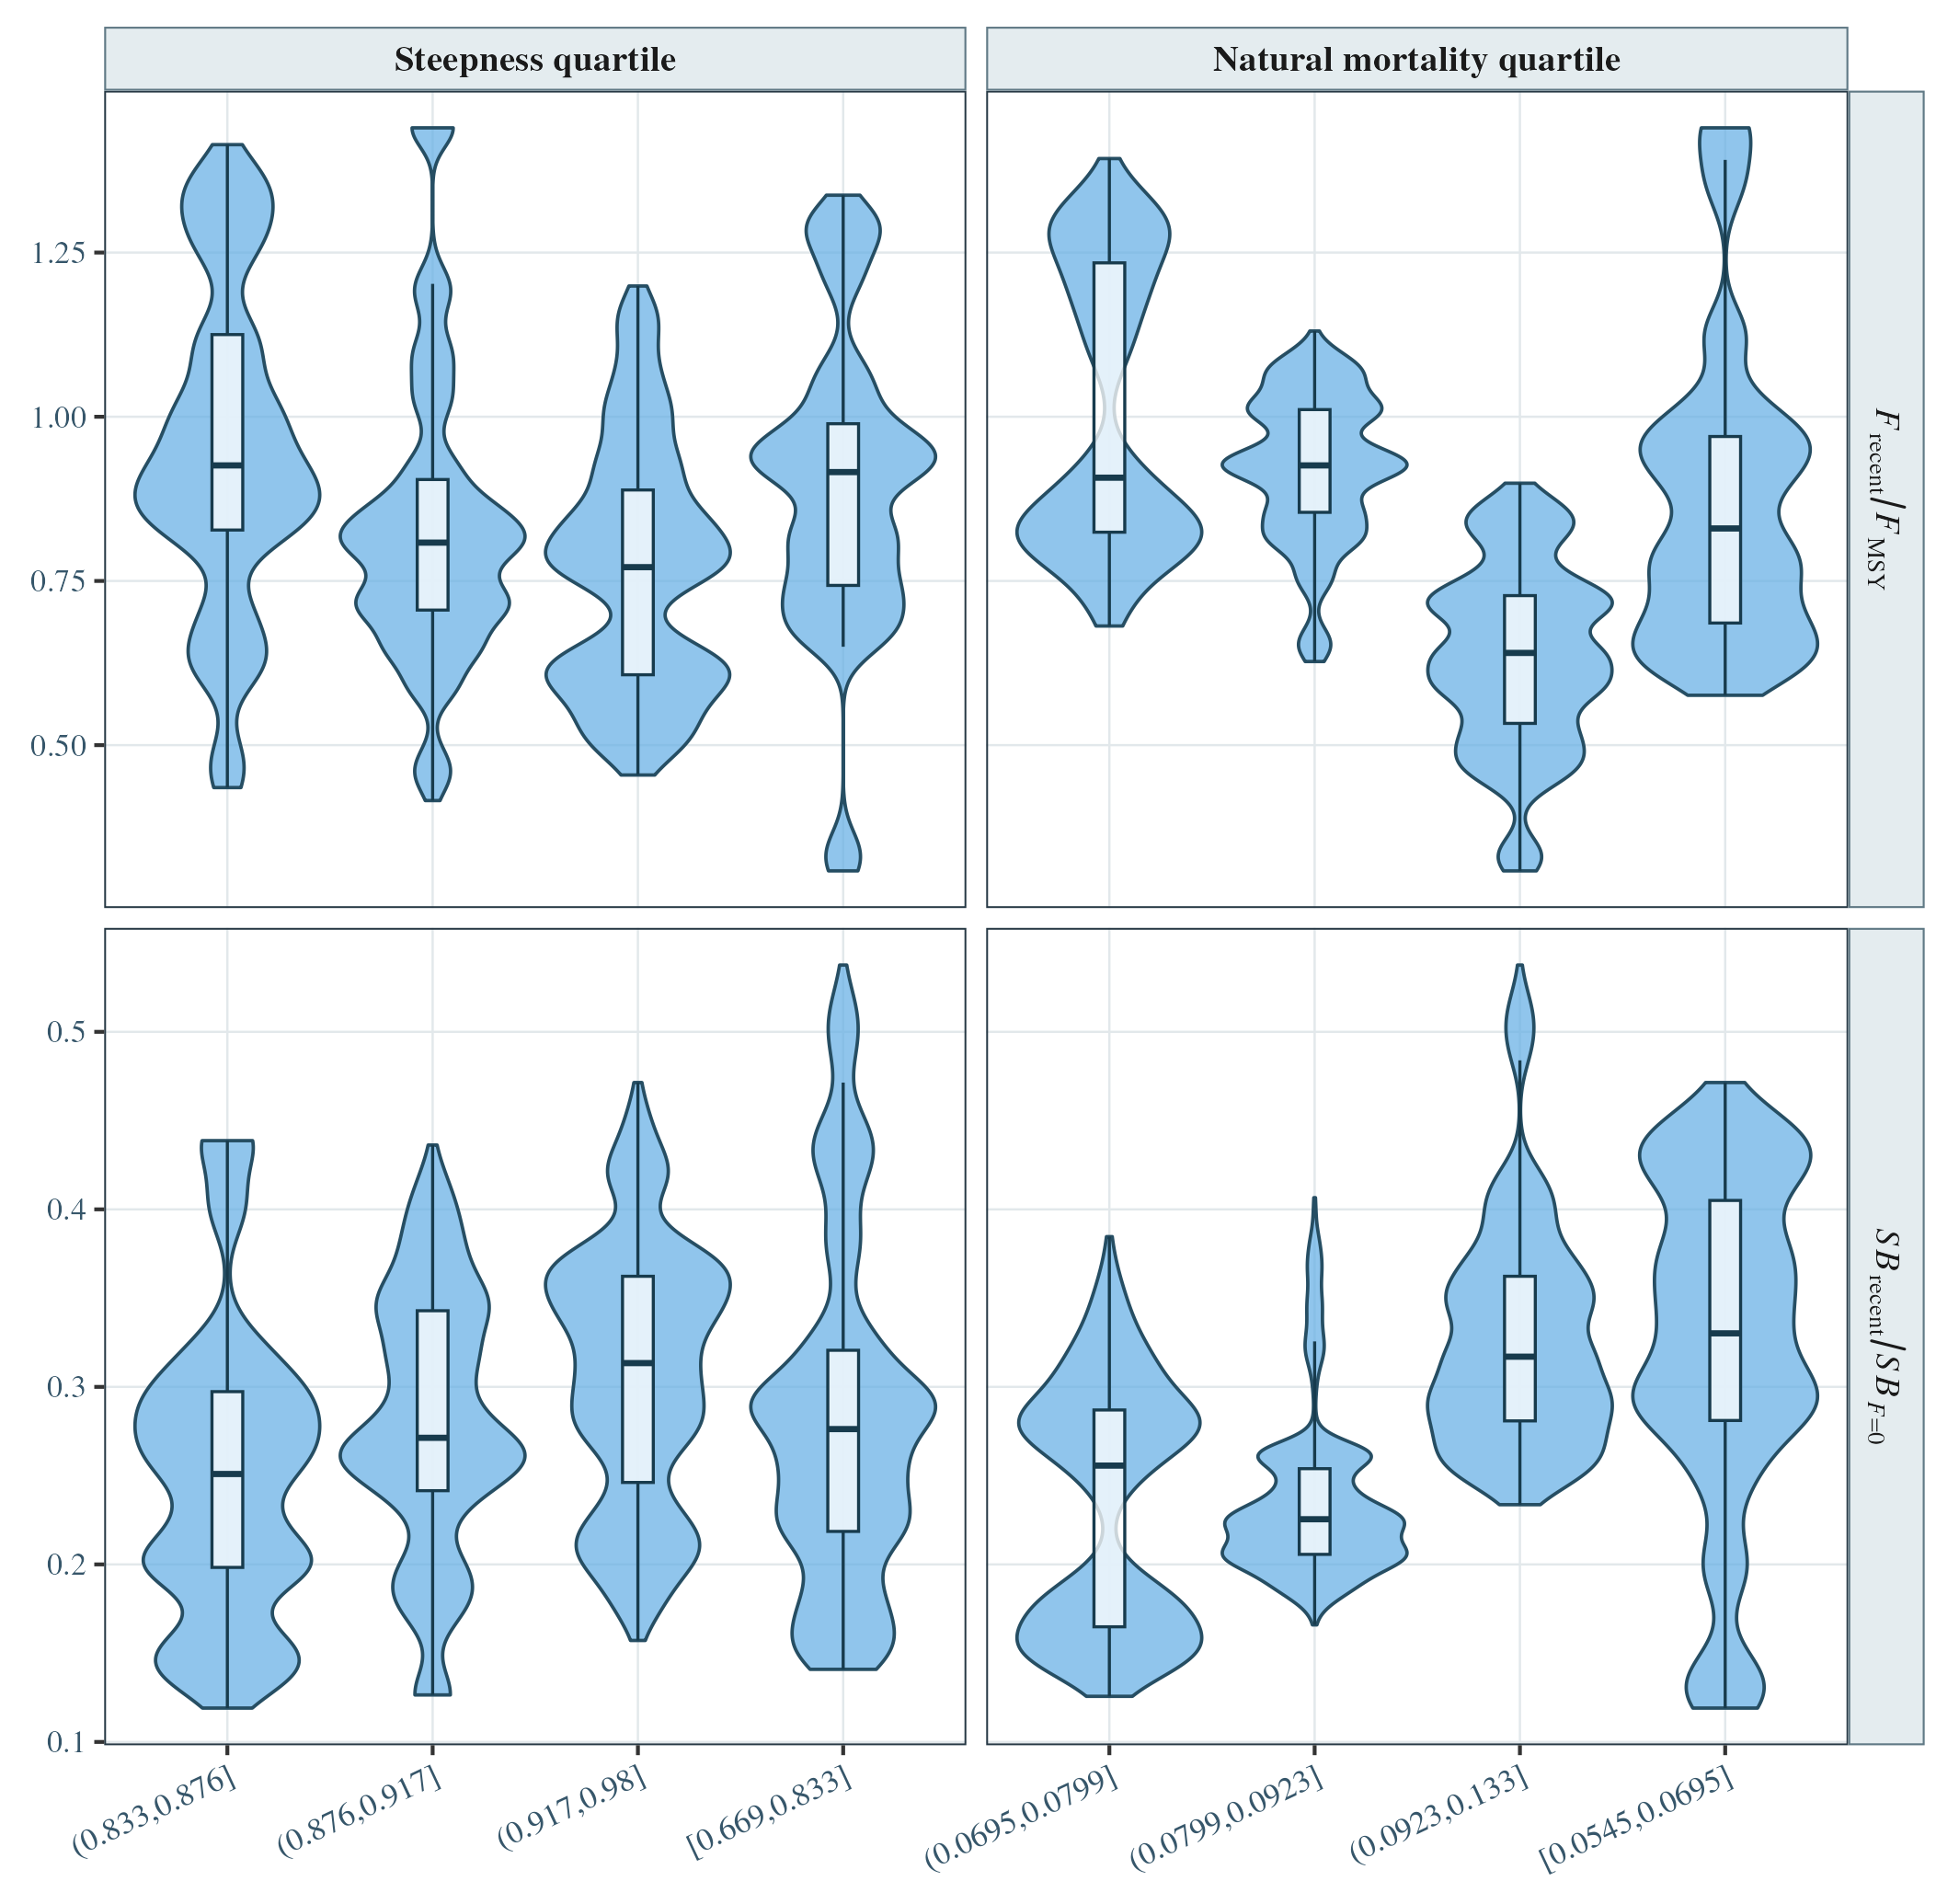
\includegraphics[width=1\linewidth,height=\textheight,keepaspectratio]{figures/management-uncertainty-continuous-axes_steep_M.png}

}

\caption{\label{fig-management-uncertainty-continuous-axes-steep-M}All-model
uncertainty distributions of \(F_{recent}\)/\(F_{MSY}\) (top) and
\(SB_{recent}\)/\(SB_{F=0}\) (bottom), grouped by quartiles of steepness
and natural mortality at the reference length. Violin width represents
density and the inset box shows the interquartile range and median. Each
model has equal total weight; PDH models contribute joint Hessian draws
and Near-PDH models contribute their central estimates. Because all
ensemble axes vary jointly, differences among groups are descriptive and
not one-factor causal effects. Open the
\href{https://pacificcommunity.github.io/ofp-sam-bet-2026-ensemble/bet-2026-ensemble-interactive-viewer.html}{interactive
ensemble viewer}.}

\end{figure}\DIFaddend %

\DIFdelbegin %DIFDELCMD < \begin{figure}[H]
%DIFDELCMD <

%DIFDELCMD < \centering{
%DIFDELCMD <

%DIFDELCMD < 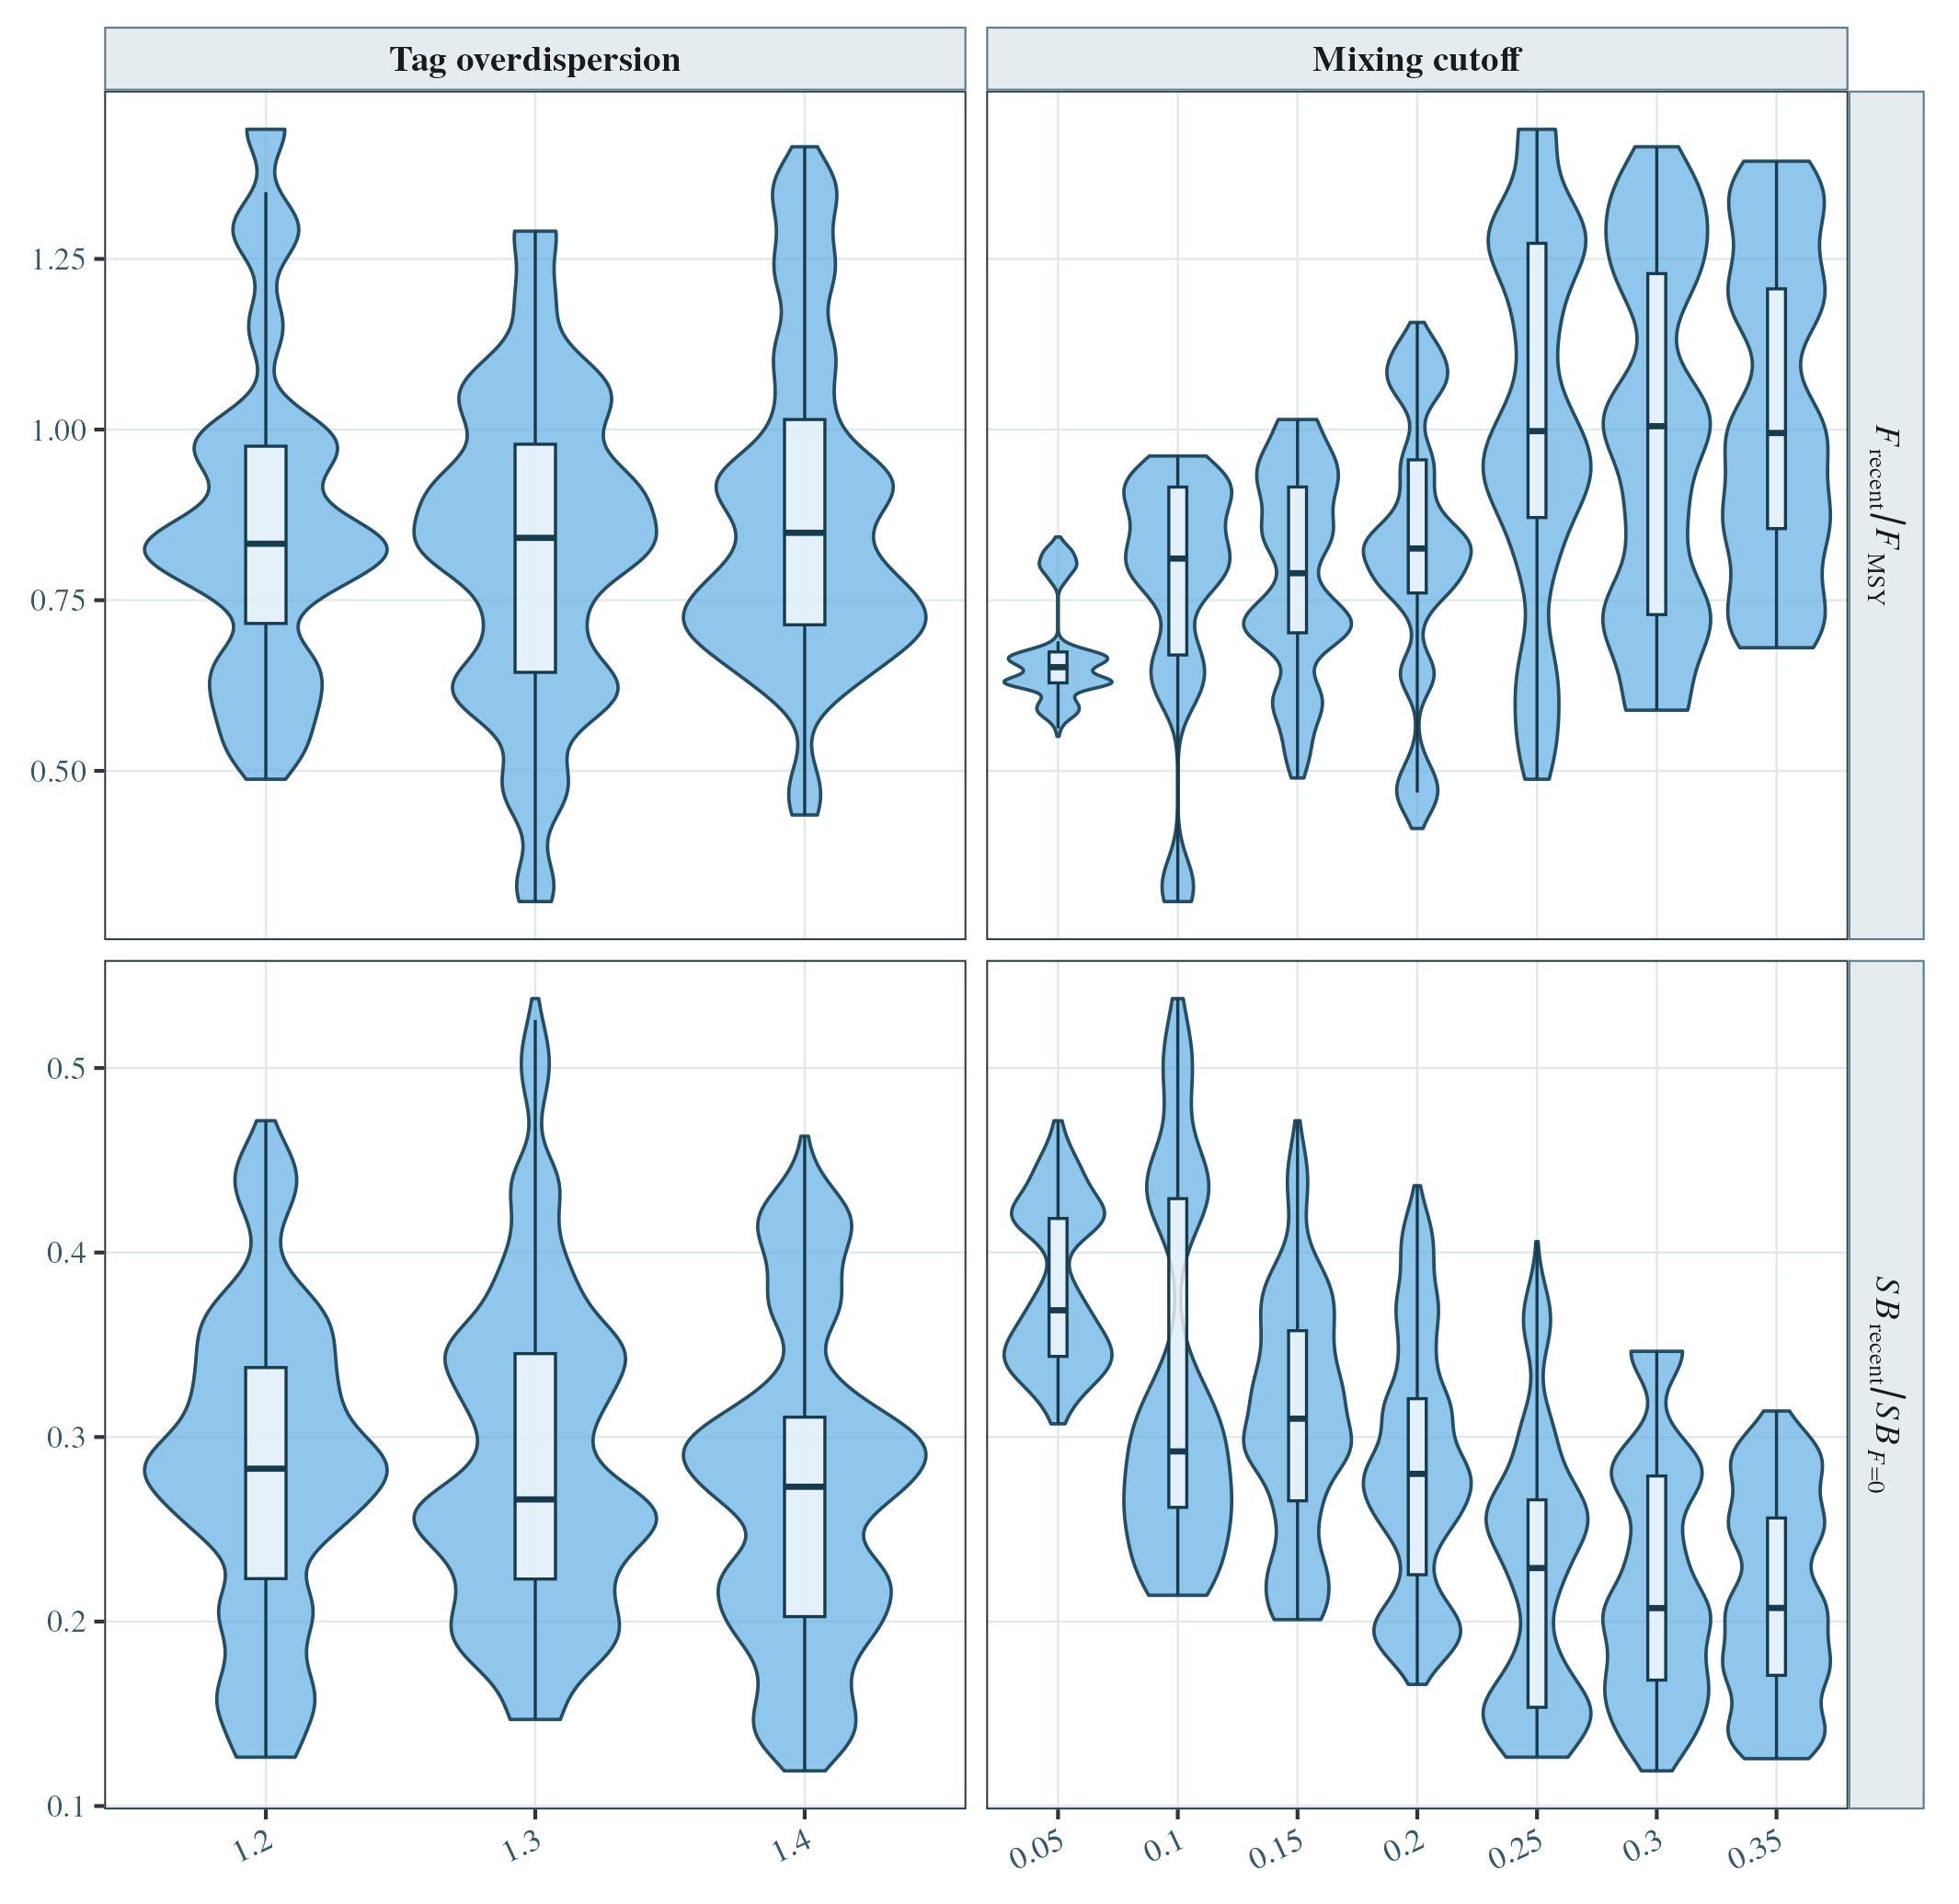
\includegraphics[width=1\linewidth,height=\textheight,keepaspectratio]{figures/management-uncertainty-discrete-axes_tau_mix.png}
%DIFDELCMD <

%DIFDELCMD < }
%DIFDELCMD <

%DIFDELCMD < \caption{\label{fig-management-uncertainty-discrete-axes-tau-mix}All-model
%DIFDELCMD < uncertainty distributions of \(F_{recent}\)/\(F_{MSY}\) (top) and
%DIFDELCMD < \(SB_{recent}\)/\(SB_{F=0}\) (bottom), grouped by fixed tag
%DIFDELCMD < overdispersion and tag-mixing cutoff. Each assessment model has equal
%DIFDELCMD < total weight. Violins show density and boxes show the median and
%DIFDELCMD < interquartile range; comparisons are marginal descriptions of a jointly
%DIFDELCMD < varying ensemble.}
%DIFDELCMD <

%DIFDELCMD < \end{figure}%%%
\DIFdelend \DIFaddbegin \begin{figure}[H]

\centering{

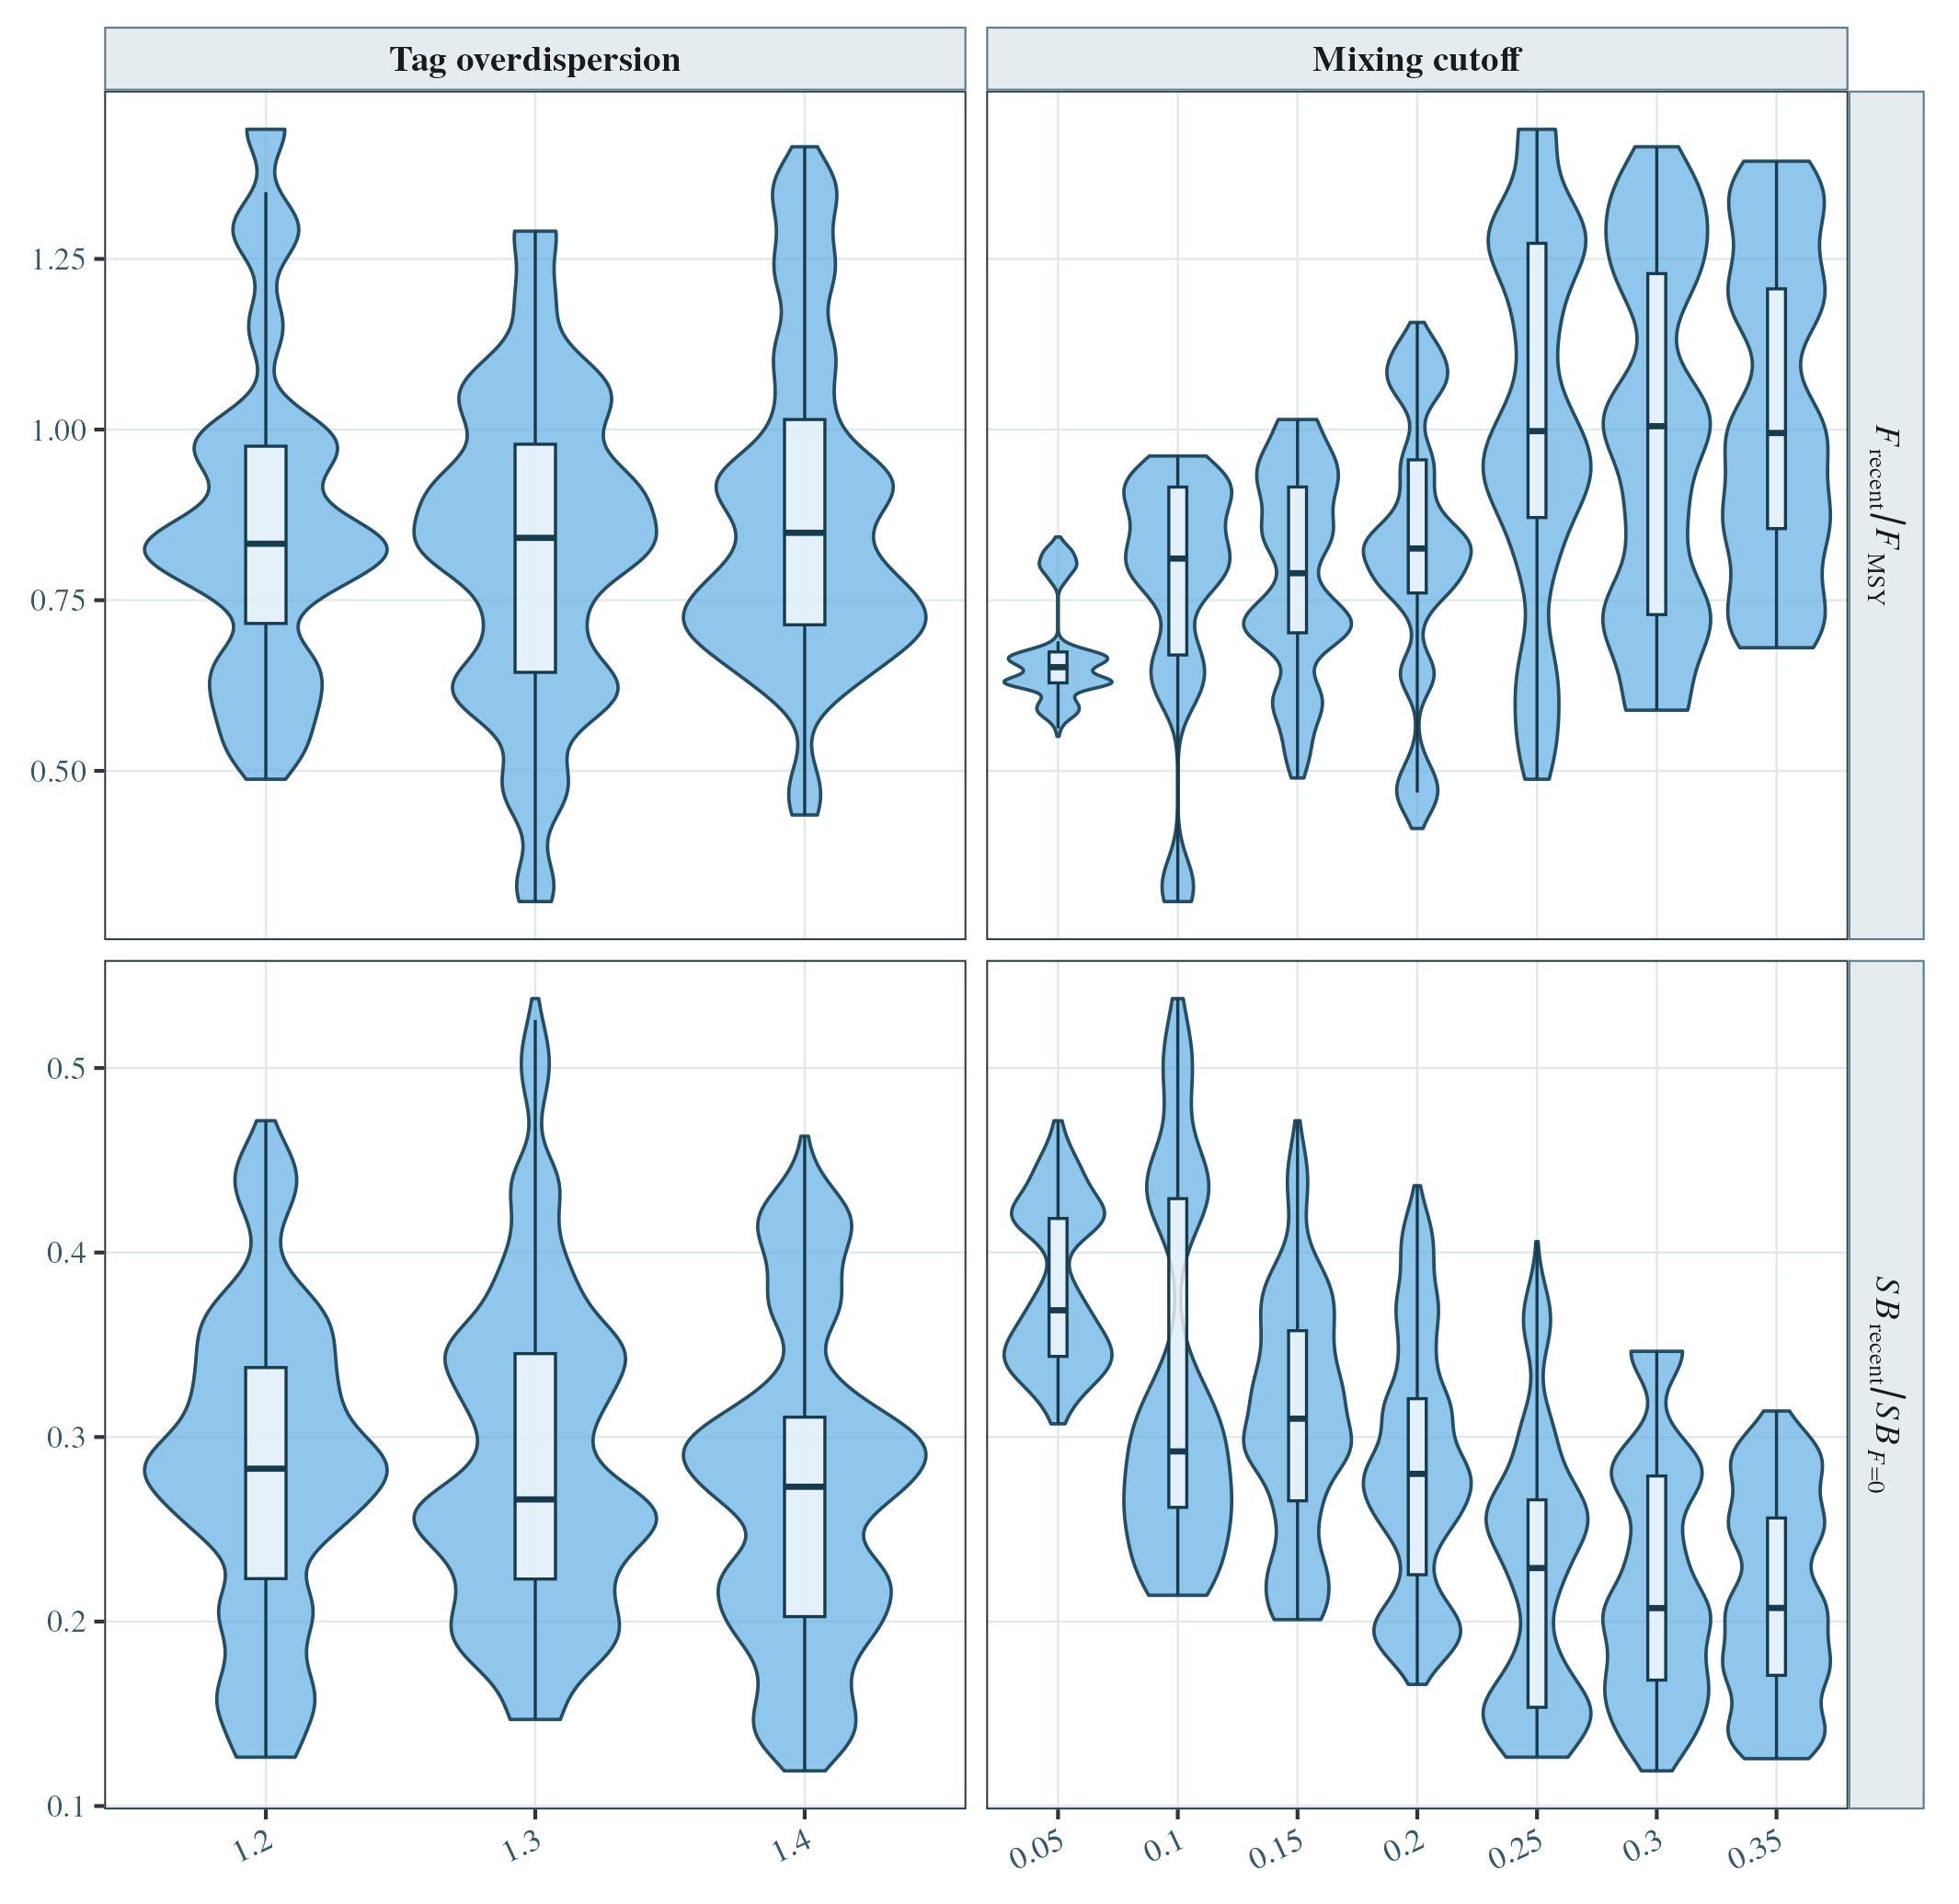
\includegraphics[width=1\linewidth,height=\textheight,keepaspectratio]{figures/management-uncertainty-discrete-axes_tau_mix.png}

}

\caption{\label{fig-management-uncertainty-discrete-axes-tau-mix}All-model
uncertainty distributions of \(F_{recent}\)/\(F_{MSY}\) (top) and
\(SB_{recent}\)/\(SB_{F=0}\) (bottom), grouped by fixed tag
overdispersion and tag-mixing cutoff. Each assessment model has equal
total weight. Violins show density and boxes show the median and
interquartile range; comparisons are marginal descriptions of a jointly
varying ensemble. Open the
\href{https://pacificcommunity.github.io/ofp-sam-bet-2026-ensemble/bet-2026-ensemble-interactive-viewer.html}{interactive
ensemble viewer}.}

\end{figure}\DIFaddend %

\DIFdelbegin %DIFDELCMD < \begin{figure}[H]
%DIFDELCMD <

%DIFDELCMD < \centering{
%DIFDELCMD <

%DIFDELCMD < 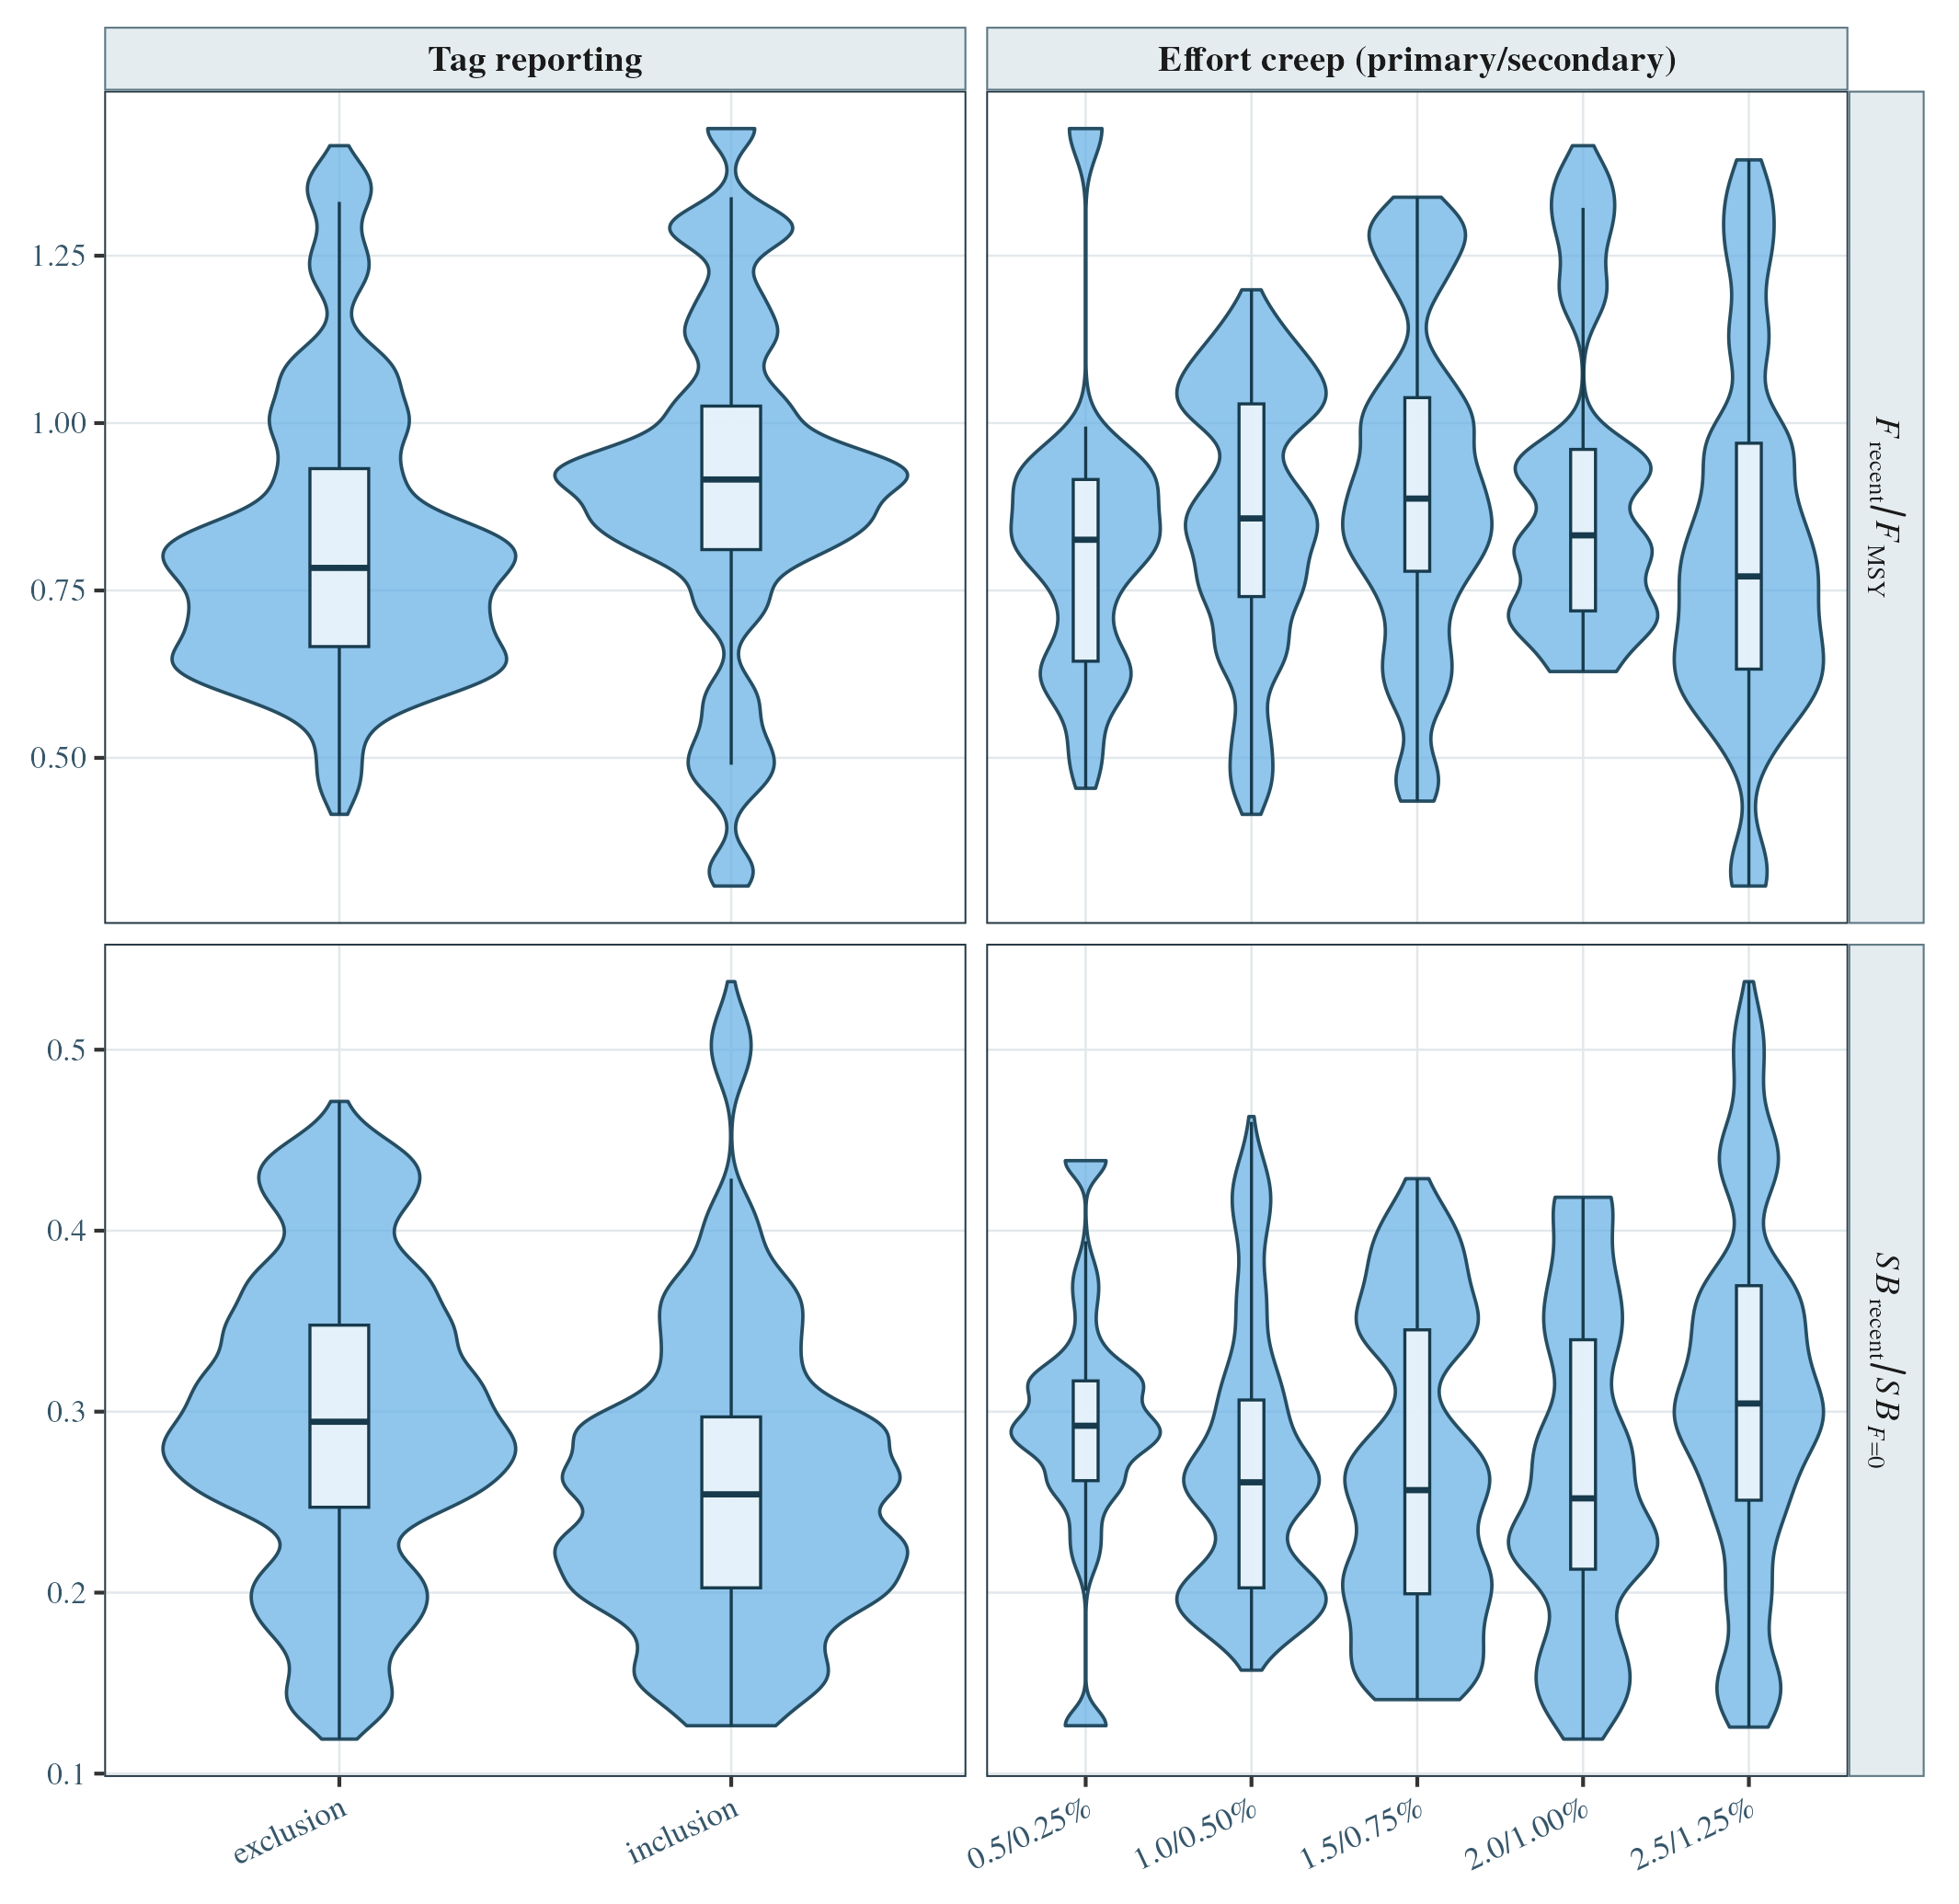
\includegraphics[width=1\linewidth,height=\textheight,keepaspectratio]{figures/management-uncertainty-discrete-axes_tag_rep_effcrp.png}
%DIFDELCMD <

%DIFDELCMD < }
%DIFDELCMD <

%DIFDELCMD < \caption{\label{fig-management-uncertainty-discrete-axes-tag-rep-effcrp}All-model
%DIFDELCMD < uncertainty distributions of \(F_{recent}\)/\(F_{MSY}\) (top) and
%DIFDELCMD < \(SB_{recent}\)/\(SB_{F=0}\) (bottom), grouped by tag-reporting
%DIFDELCMD < treatment and paired annual effort-creep rates. Each assessment model
%DIFDELCMD < has equal total weight. Violins show density and boxes show the median
%DIFDELCMD < and interquartile range; comparisons are marginal descriptions rather
%DIFDELCMD < than controlled one-factor sensitivities.}
%DIFDELCMD <

%DIFDELCMD < \end{figure}%%%
\DIFdelend \DIFaddbegin \begin{figure}[H]

\centering{

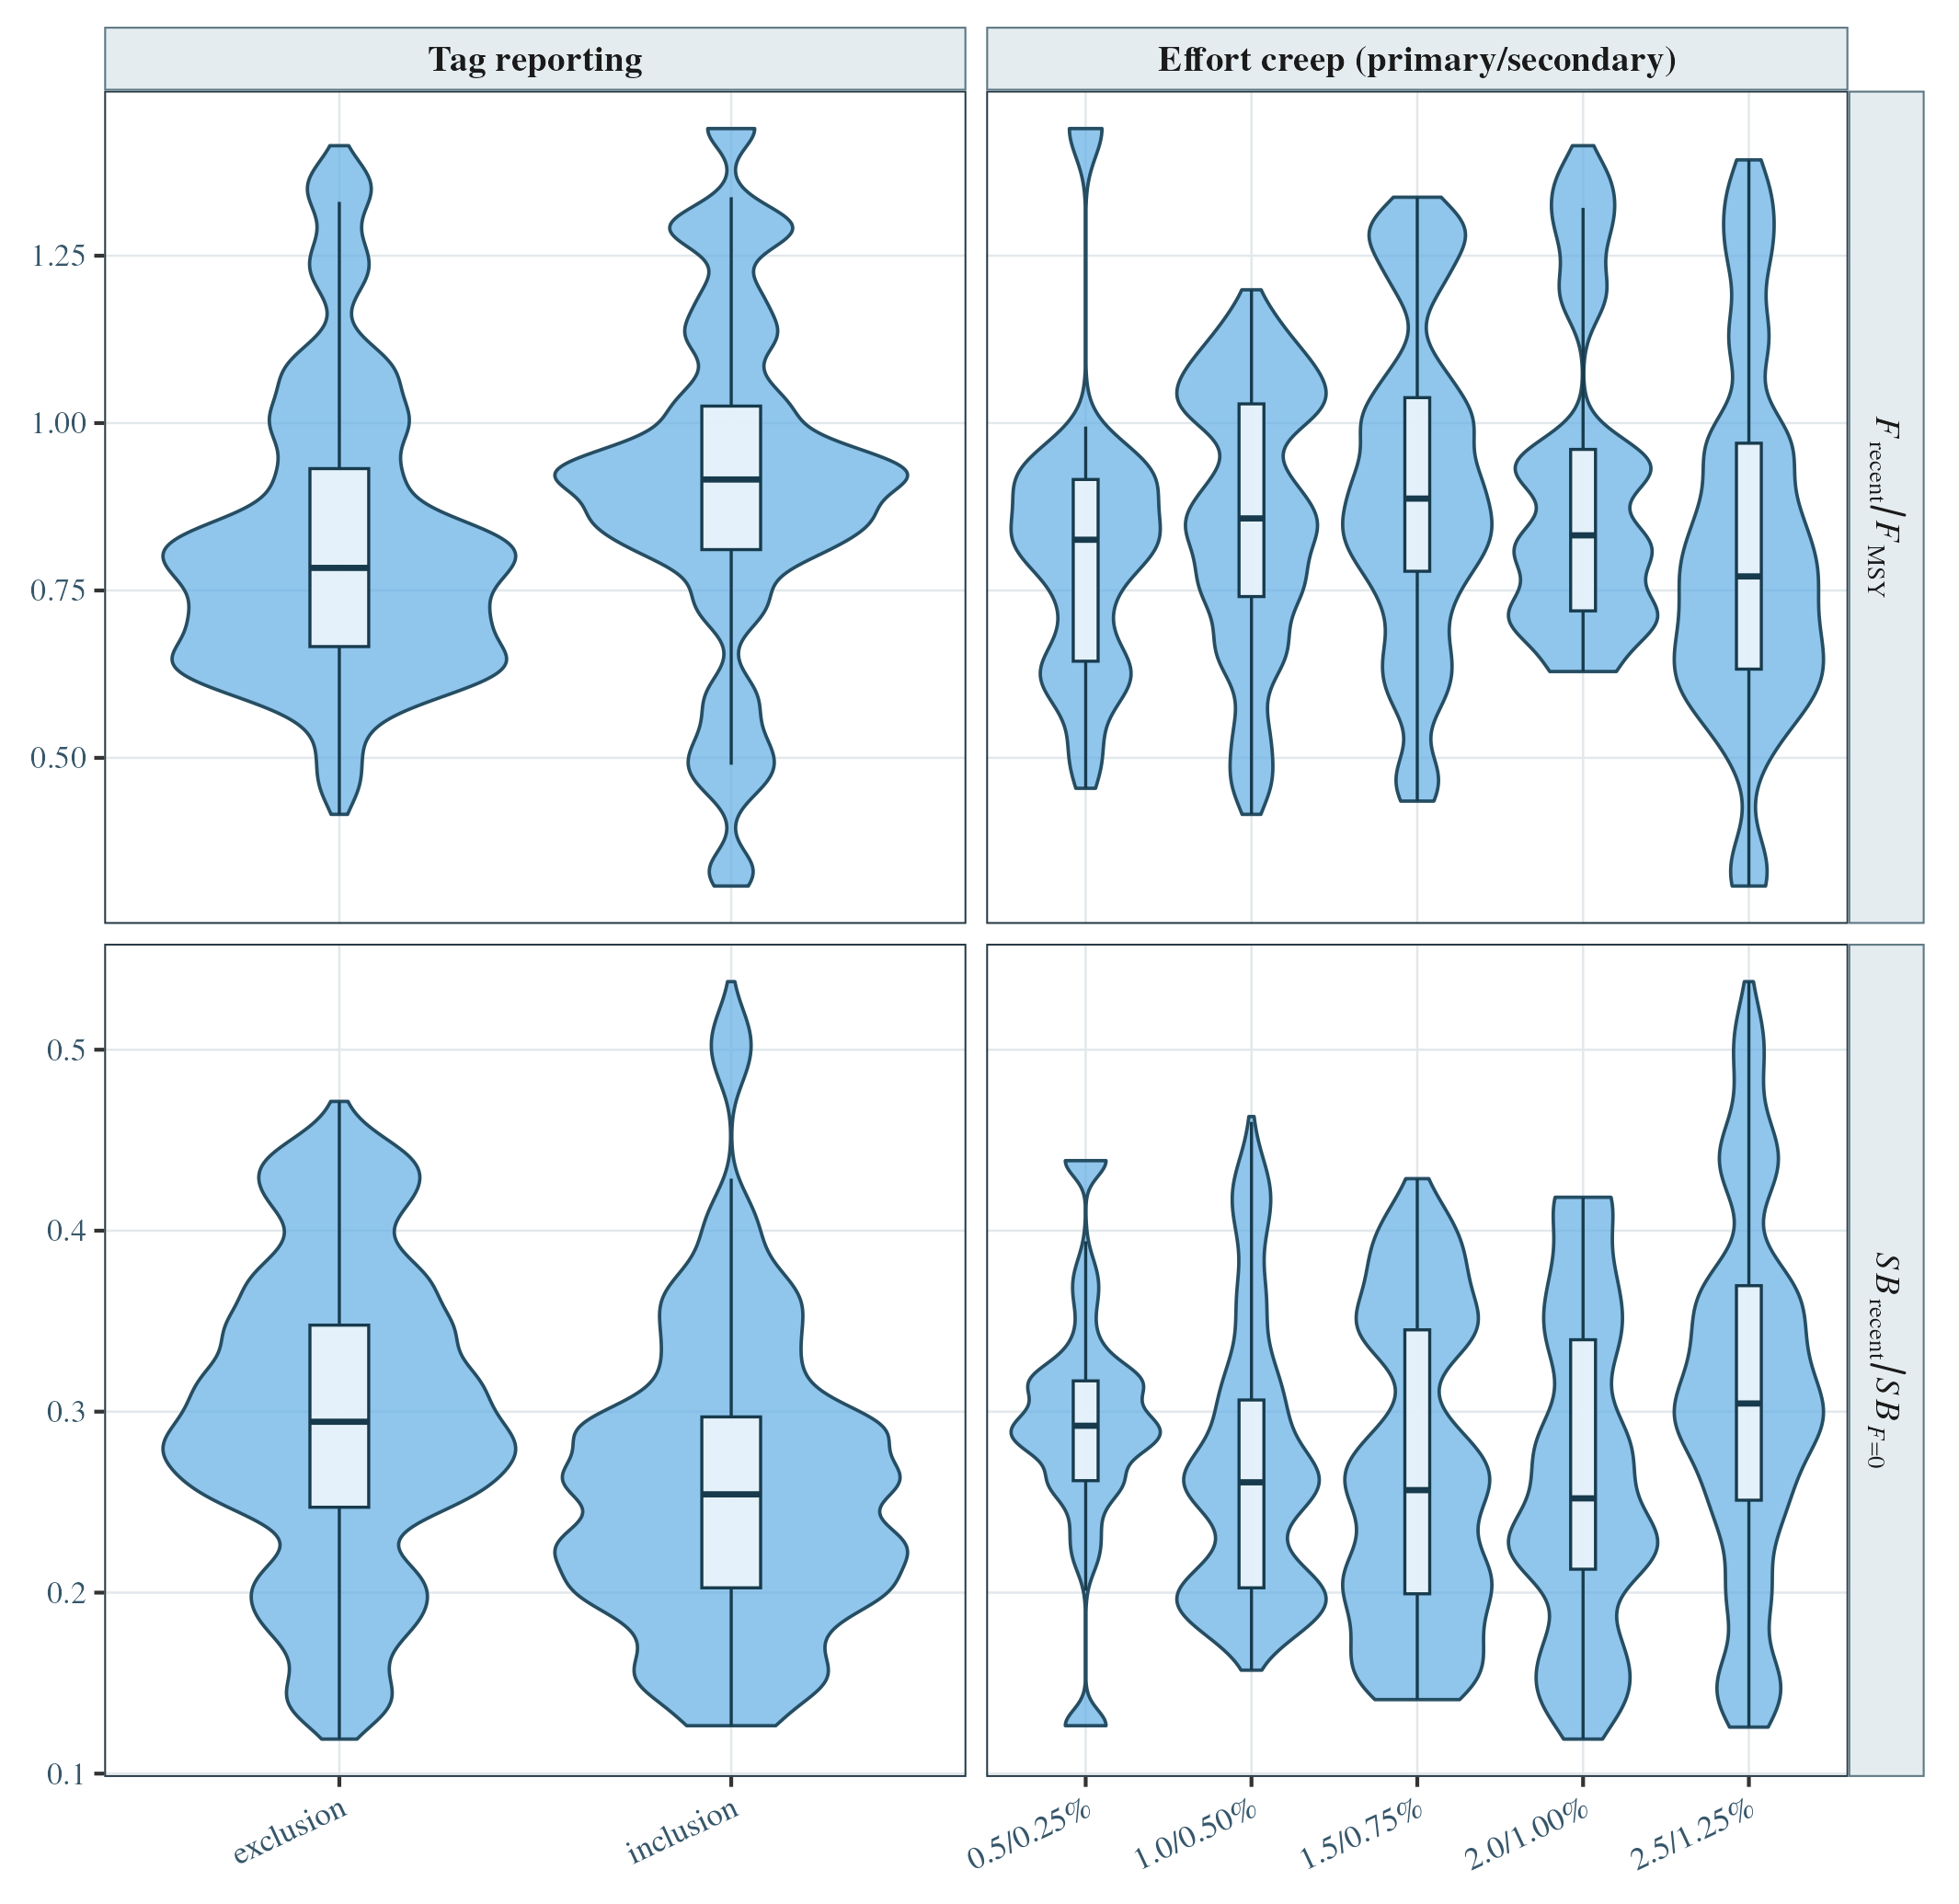
\includegraphics[width=1\linewidth,height=\textheight,keepaspectratio]{figures/management-uncertainty-discrete-axes_tag_rep_effcrp.png}

}

\caption{\label{fig-management-uncertainty-discrete-axes-tag-rep-effcrp}All-model
uncertainty distributions of \(F_{recent}\)/\(F_{MSY}\) (top) and
\(SB_{recent}\)/\(SB_{F=0}\) (bottom), grouped by tag-reporting
treatment and paired annual effort-creep rates. Each assessment model
has equal total weight. Violins show density and boxes show the median
and interquartile range; comparisons are marginal descriptions rather
than controlled one-factor sensitivities. Open the
\href{https://pacificcommunity.github.io/ofp-sam-bet-2026-ensemble/bet-2026-ensemble-interactive-viewer.html}{interactive
ensemble viewer}.}

\end{figure}\DIFaddend %

\DIFdelbegin %DIFDELCMD < \begin{figure}[H]
%DIFDELCMD <

%DIFDELCMD < \centering{
%DIFDELCMD <

%DIFDELCMD < 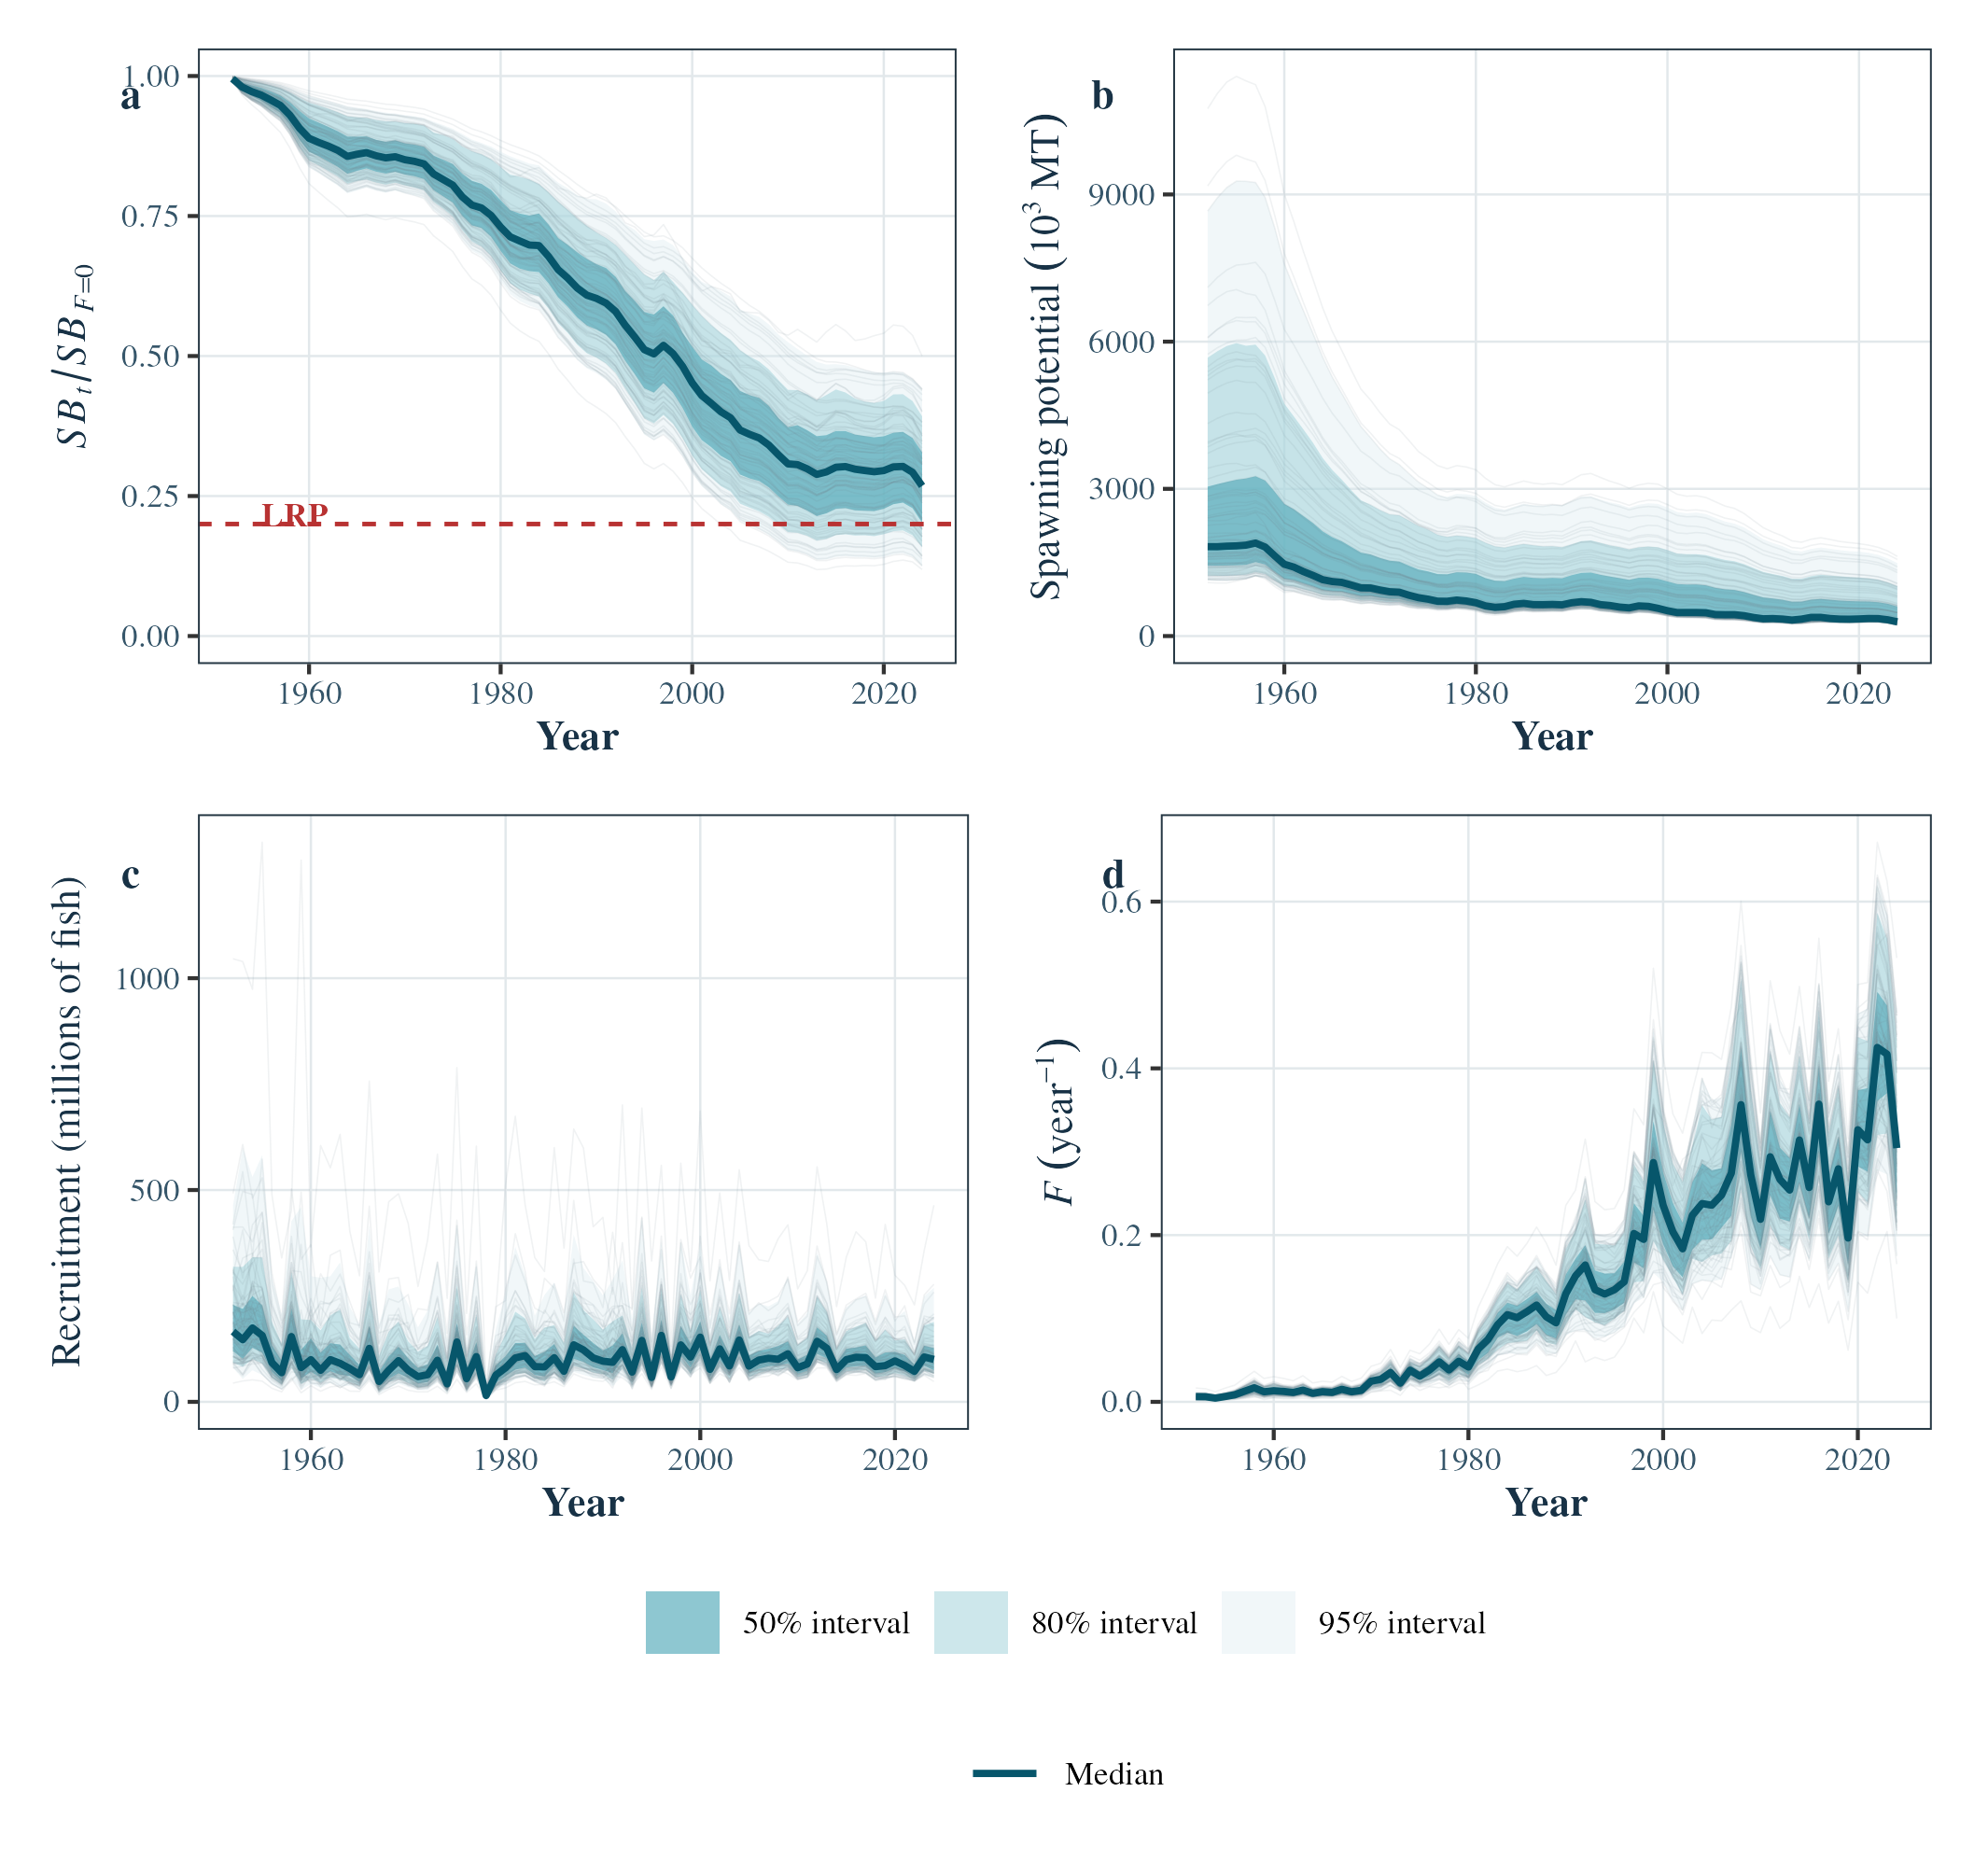
\includegraphics[width=1\linewidth,height=\textheight,keepaspectratio]{figures/ensemble_est_uncert_ribbon.png}
%DIFDELCMD <

%DIFDELCMD < }
%DIFDELCMD <

%DIFDELCMD < \caption{\label{fig-ensemble-est-uncert-ribbon}Ribbon plots of estimated
%DIFDELCMD < dynamic spawning depletion (Top left) and spawning potential (Top
%DIFDELCMD < right), recruitment (Bottom left) and fishing mortality (Bottom right)
%DIFDELCMD < for the 80 models retained for the uncertainty ensemble including the
%DIFDELCMD < estimation uncertainty. The median and pointwise central 50\%, 80\% and
%DIFDELCMD < 95\% intervals use the uncertainty samples available for each quantity.
%DIFDELCMD < Grey lines show central model trajectories.}
%DIFDELCMD <

%DIFDELCMD < \end{figure}%%%
\DIFdelend \DIFaddbegin \begin{figure}[H]

\centering{

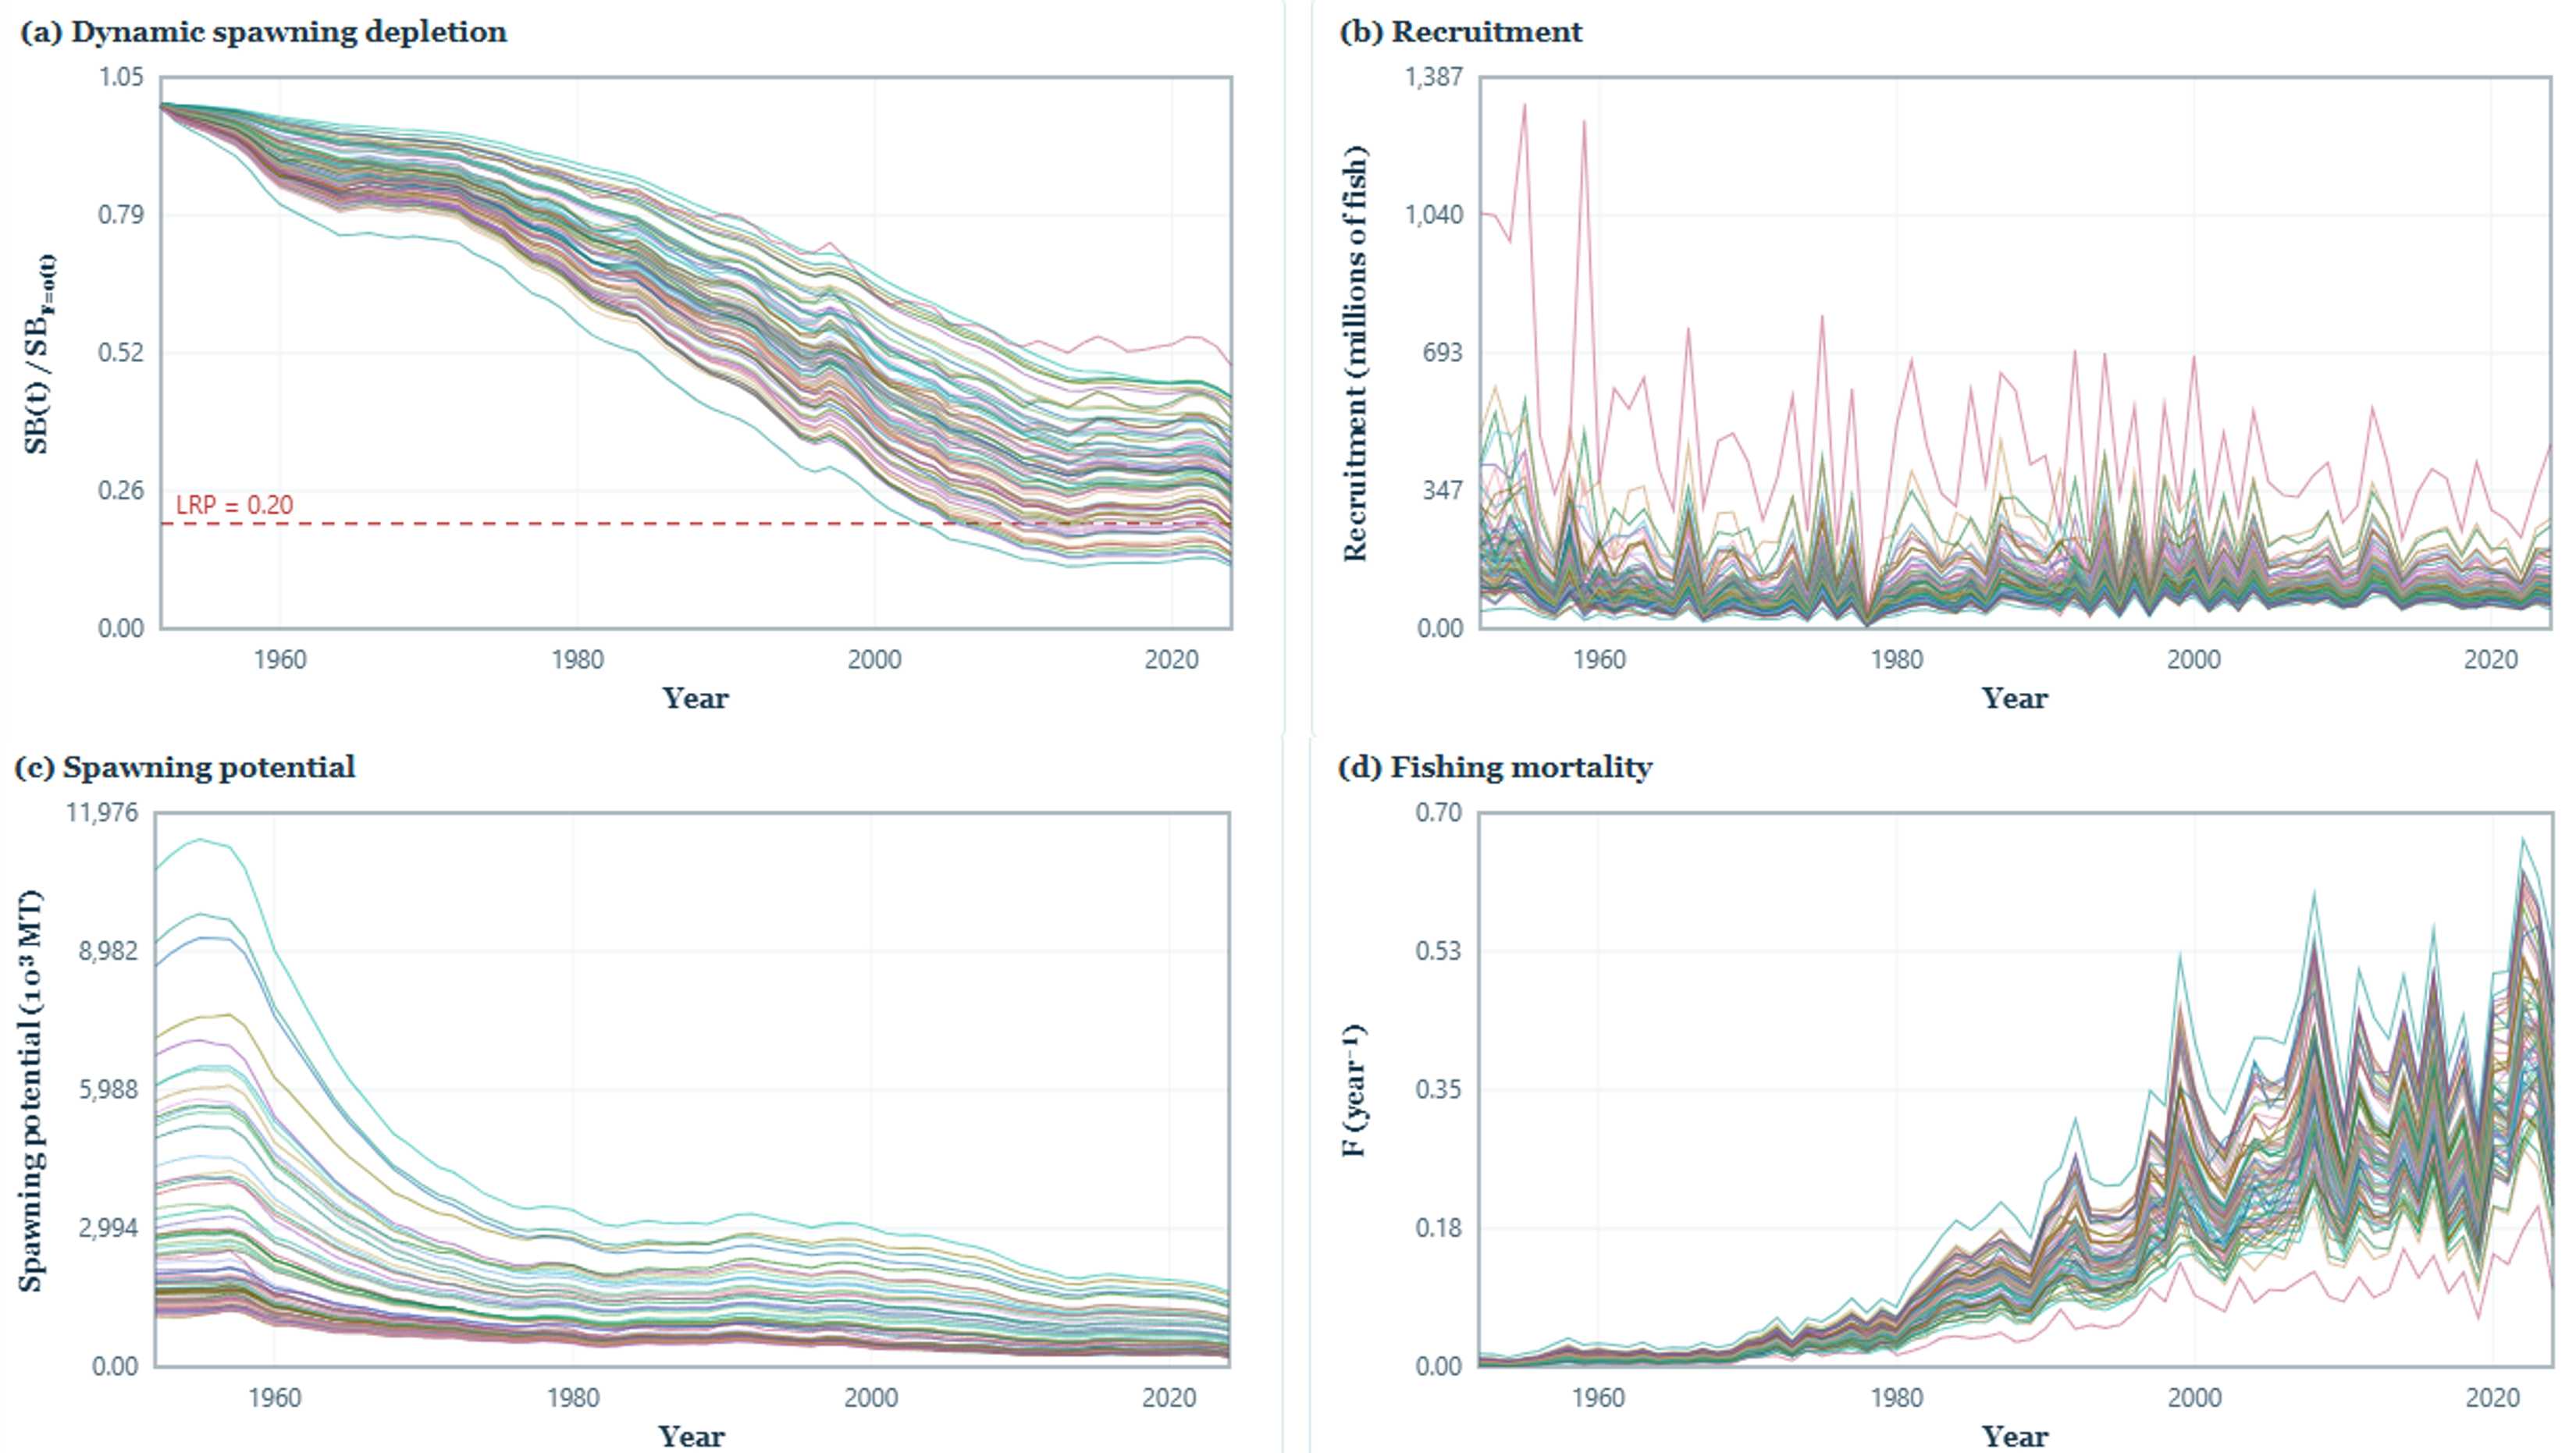
\includegraphics[width=1\linewidth,height=\textheight,keepaspectratio]{figures/ensemble_individual.png}

}

\caption{\label{fig-ensemble-individual}Estimated dynamic spawning
depletion (top left), spawning potential (bottom left), recruitment (top
right) and fishing mortality (bottom right) for the 80 individual models
retained for the uncertainty ensemble. Open the
\href{https://pacificcommunity.github.io/ofp-sam-bet-2026-ensemble/bet-2026-ensemble-interactive-viewer.html}{interactive
ensemble viewer}.}

\end{figure}\DIFaddend %

\DIFdelbegin %DIFDELCMD < \begin{figure}[H]
%DIFDELCMD <

%DIFDELCMD < \centering{
%DIFDELCMD <

%DIFDELCMD < 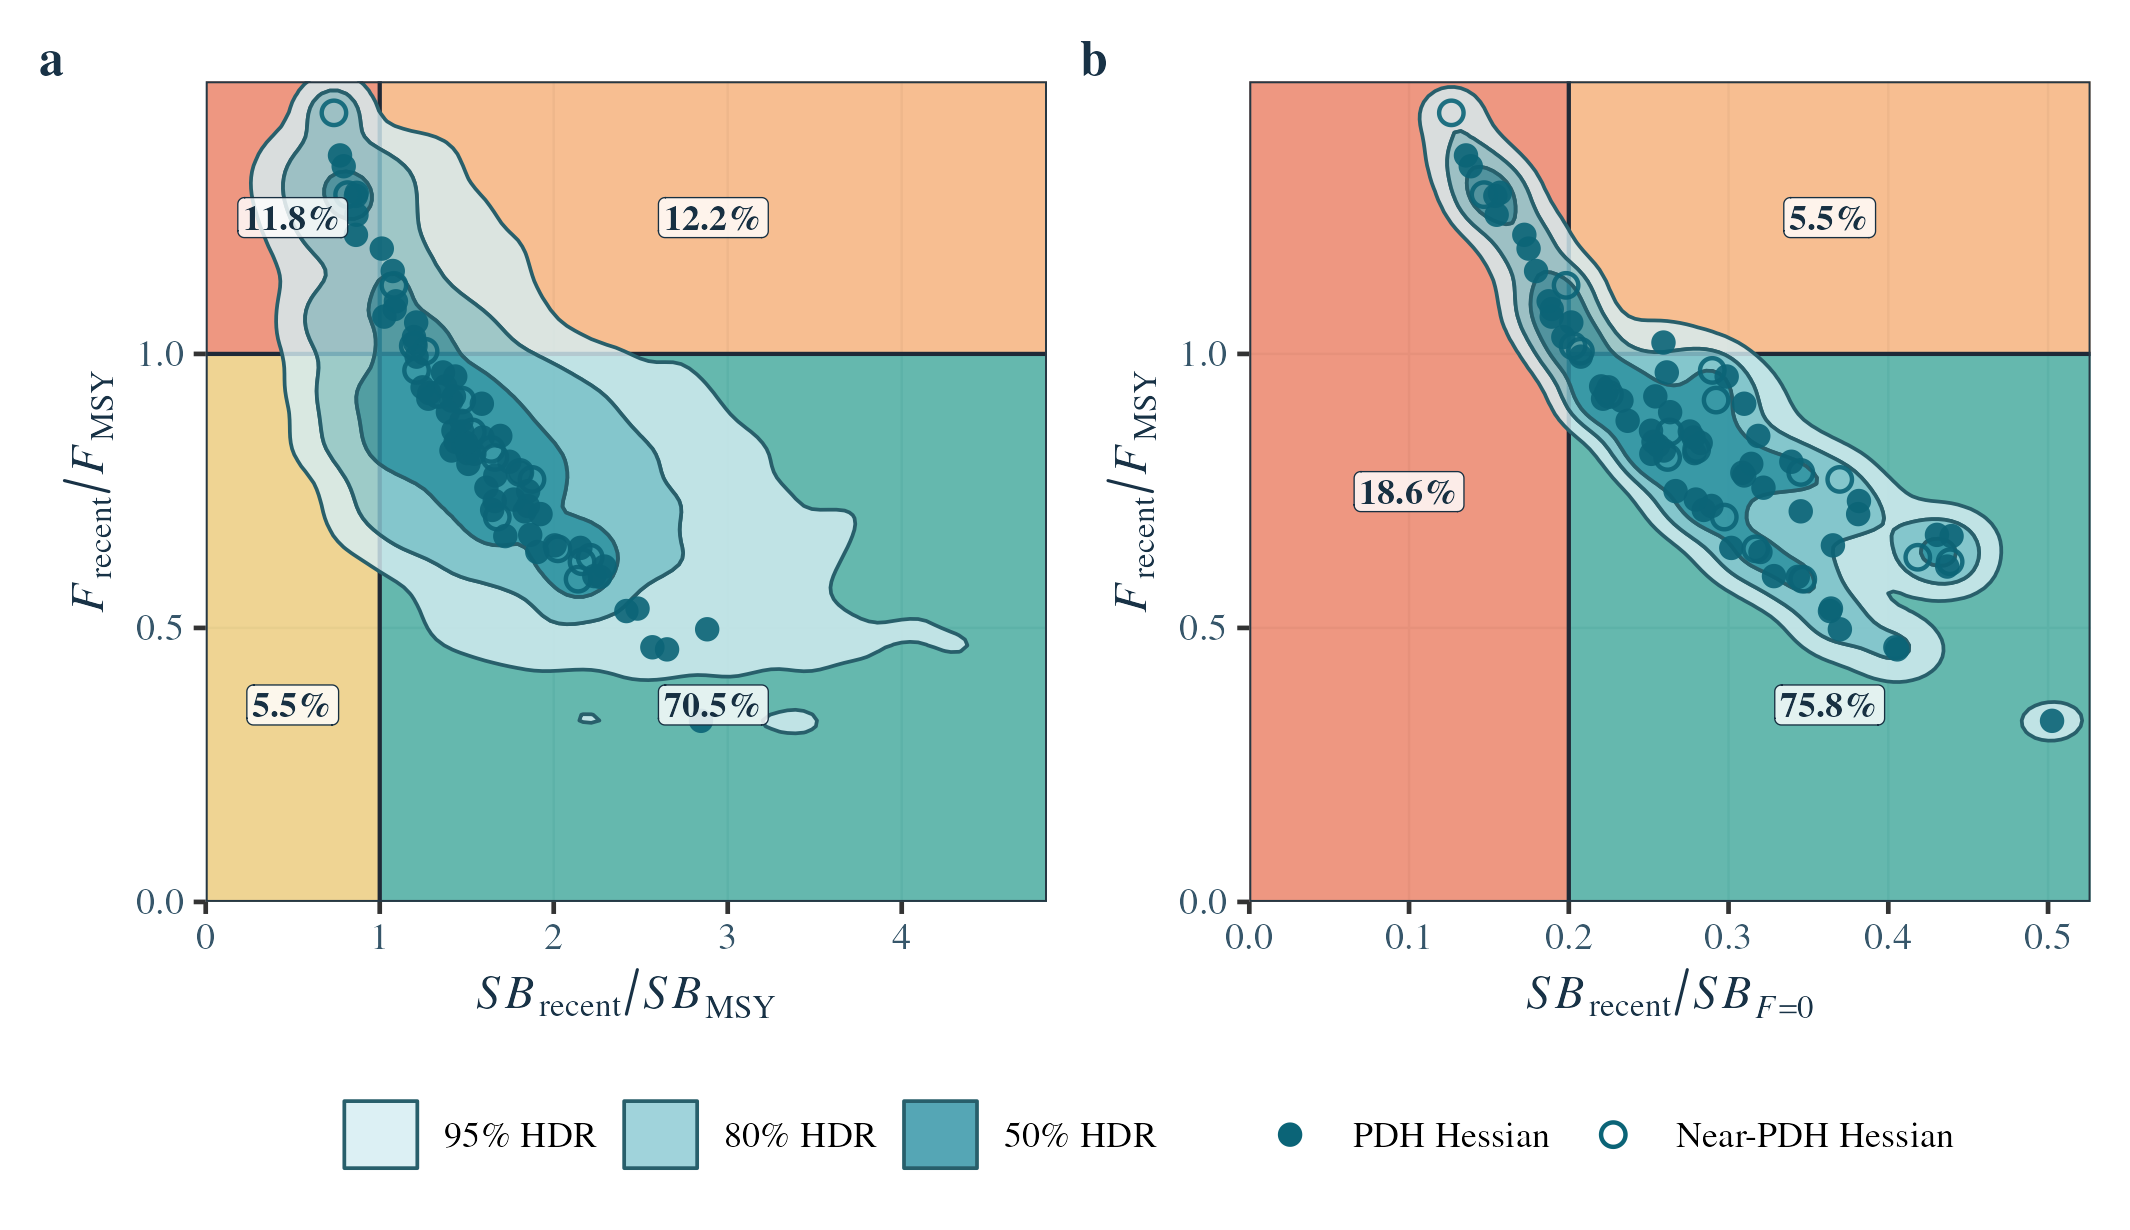
\includegraphics[width=1\linewidth,height=\textheight,keepaspectratio]{figures/combined_kobe_majuro_status.png}
%DIFDELCMD <

%DIFDELCMD < }
%DIFDELCMD <

%DIFDELCMD < \caption{\label{fig-combined-kobe-majuro-status}Stock status based on
%DIFDELCMD < \(SB_{recent}\)/\(SB_{F=0}\) (SBrecent 2021--2024) and
%DIFDELCMD < \(F_{recent}\)/\(F_{MSY}\) (Frecent 2020--2023). Panel (a) Kobe: is
%DIFDELCMD < relative to \(SB_{recent}\)/\(SB_{MSY}\) and \(F_{recent}\)/\(F_{MSY}\)
%DIFDELCMD < panel (b) Majuro: \(SB_{recent}\)/\(SB_{F=0}\) and
%DIFDELCMD < \(F_{recent}\)/\(F_{MSY}\) with the LRP of \(SB_{recent}\)/\(SB_{F=0}\)
%DIFDELCMD < = 0.20. Points are the 80 model estimates; filled and open symbols
%DIFDELCMD < distinguish PDH and Near-PDH fits. Nested 50\%, 80\% and 95\% HDRs
%DIFDELCMD < combine structural uncertainty with available joint Hessian uncertainty.
%DIFDELCMD < Background colours follow the Kobe four-category and Majuro
%DIFDELCMD < three-category definitions. Labels give the probability in each category
%DIFDELCMD < from the same equal-model-weight distribution used for the combined
%DIFDELCMD < HDRs.}
%DIFDELCMD <

%DIFDELCMD < \end{figure}%%%
\DIFdelend \DIFaddbegin \begin{figure}[H]

\centering{

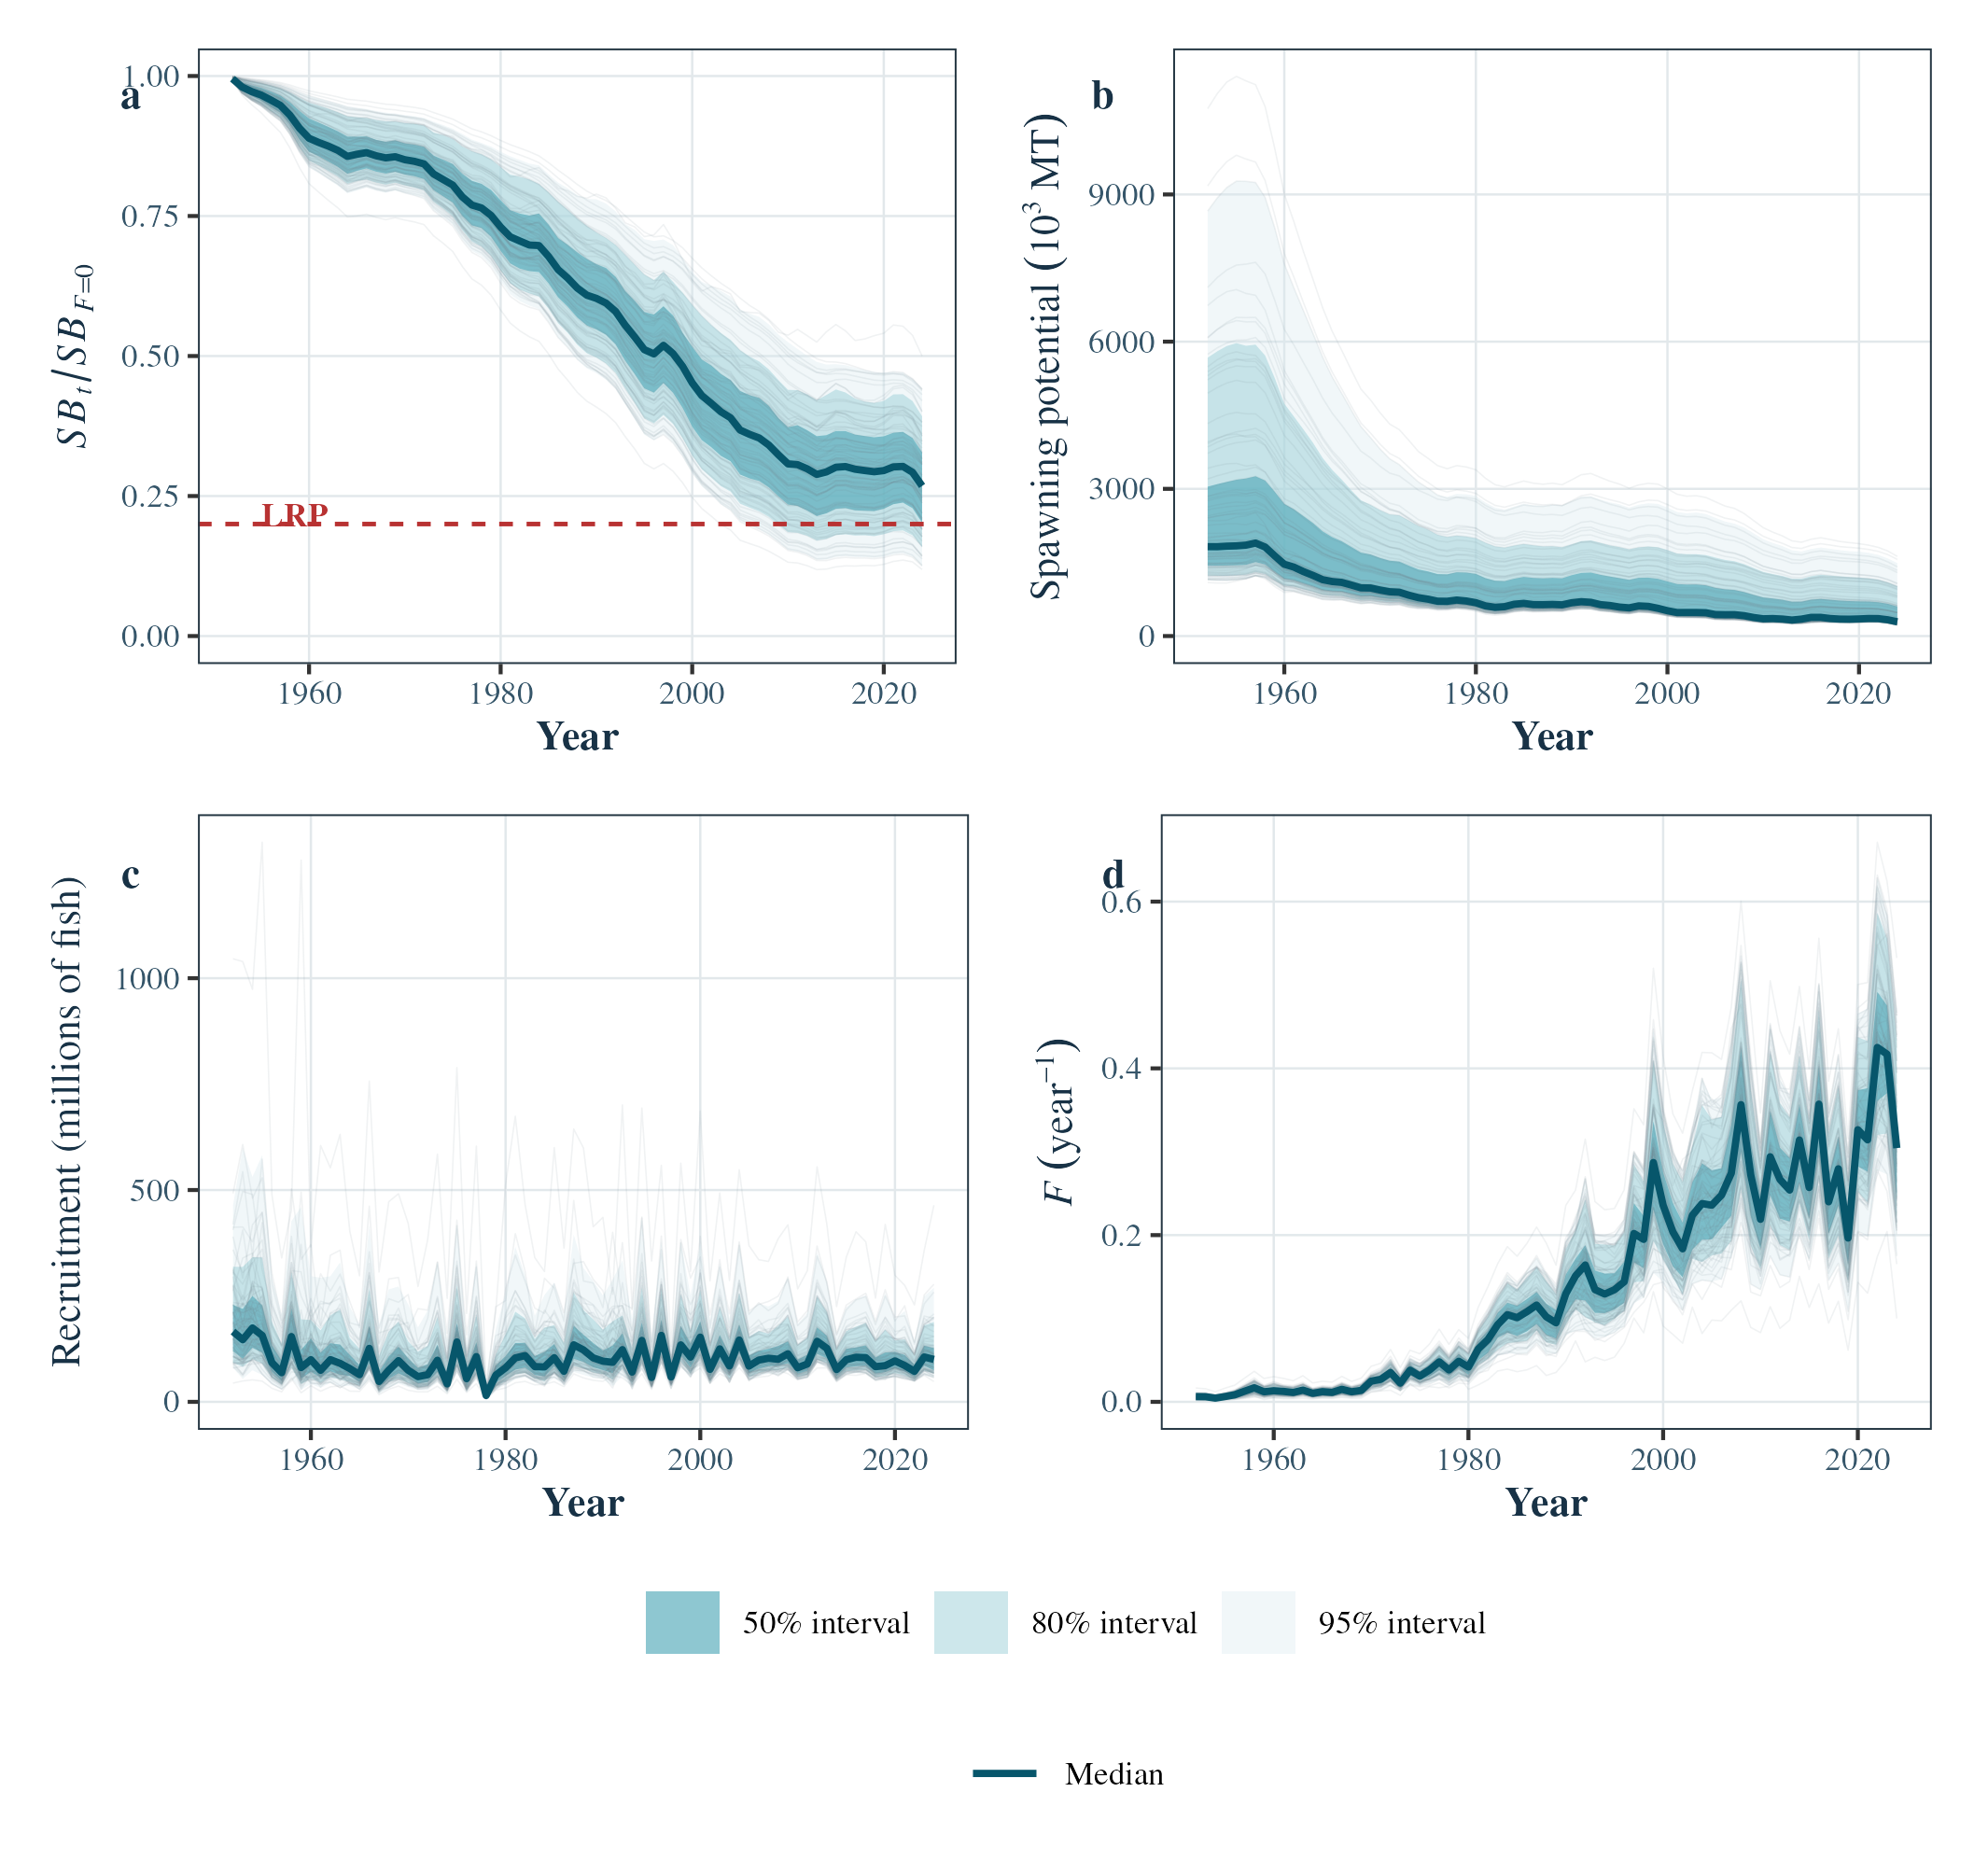
\includegraphics[width=1\linewidth,height=\textheight,keepaspectratio]{figures/ensemble_est_uncert_ribbon.png}

}

\caption{\label{fig-ensemble-est-uncert-ribbon}Ribbon plots of estimated
dynamic spawning depletion (Top left) and spawning potential (Top
right), recruitment (Bottom left) and fishing mortality (Bottom right)
for the 80 models retained for the uncertainty ensemble including the
estimation uncertainty. The median and pointwise central 50\%, 80\% and
95\% intervals use the uncertainty samples available for each quantity.
Grey lines show central model trajectories. Open the
\href{https://pacificcommunity.github.io/ofp-sam-bet-2026-ensemble/bet-2026-ensemble-interactive-viewer.html}{interactive
ensemble viewer}.}

\end{figure}\DIFaddend %

\DIFdelbegin %DIFDELCMD < \begin{figure}[H]
%DIFDELCMD <

%DIFDELCMD < \centering{
%DIFDELCMD <

%DIFDELCMD < 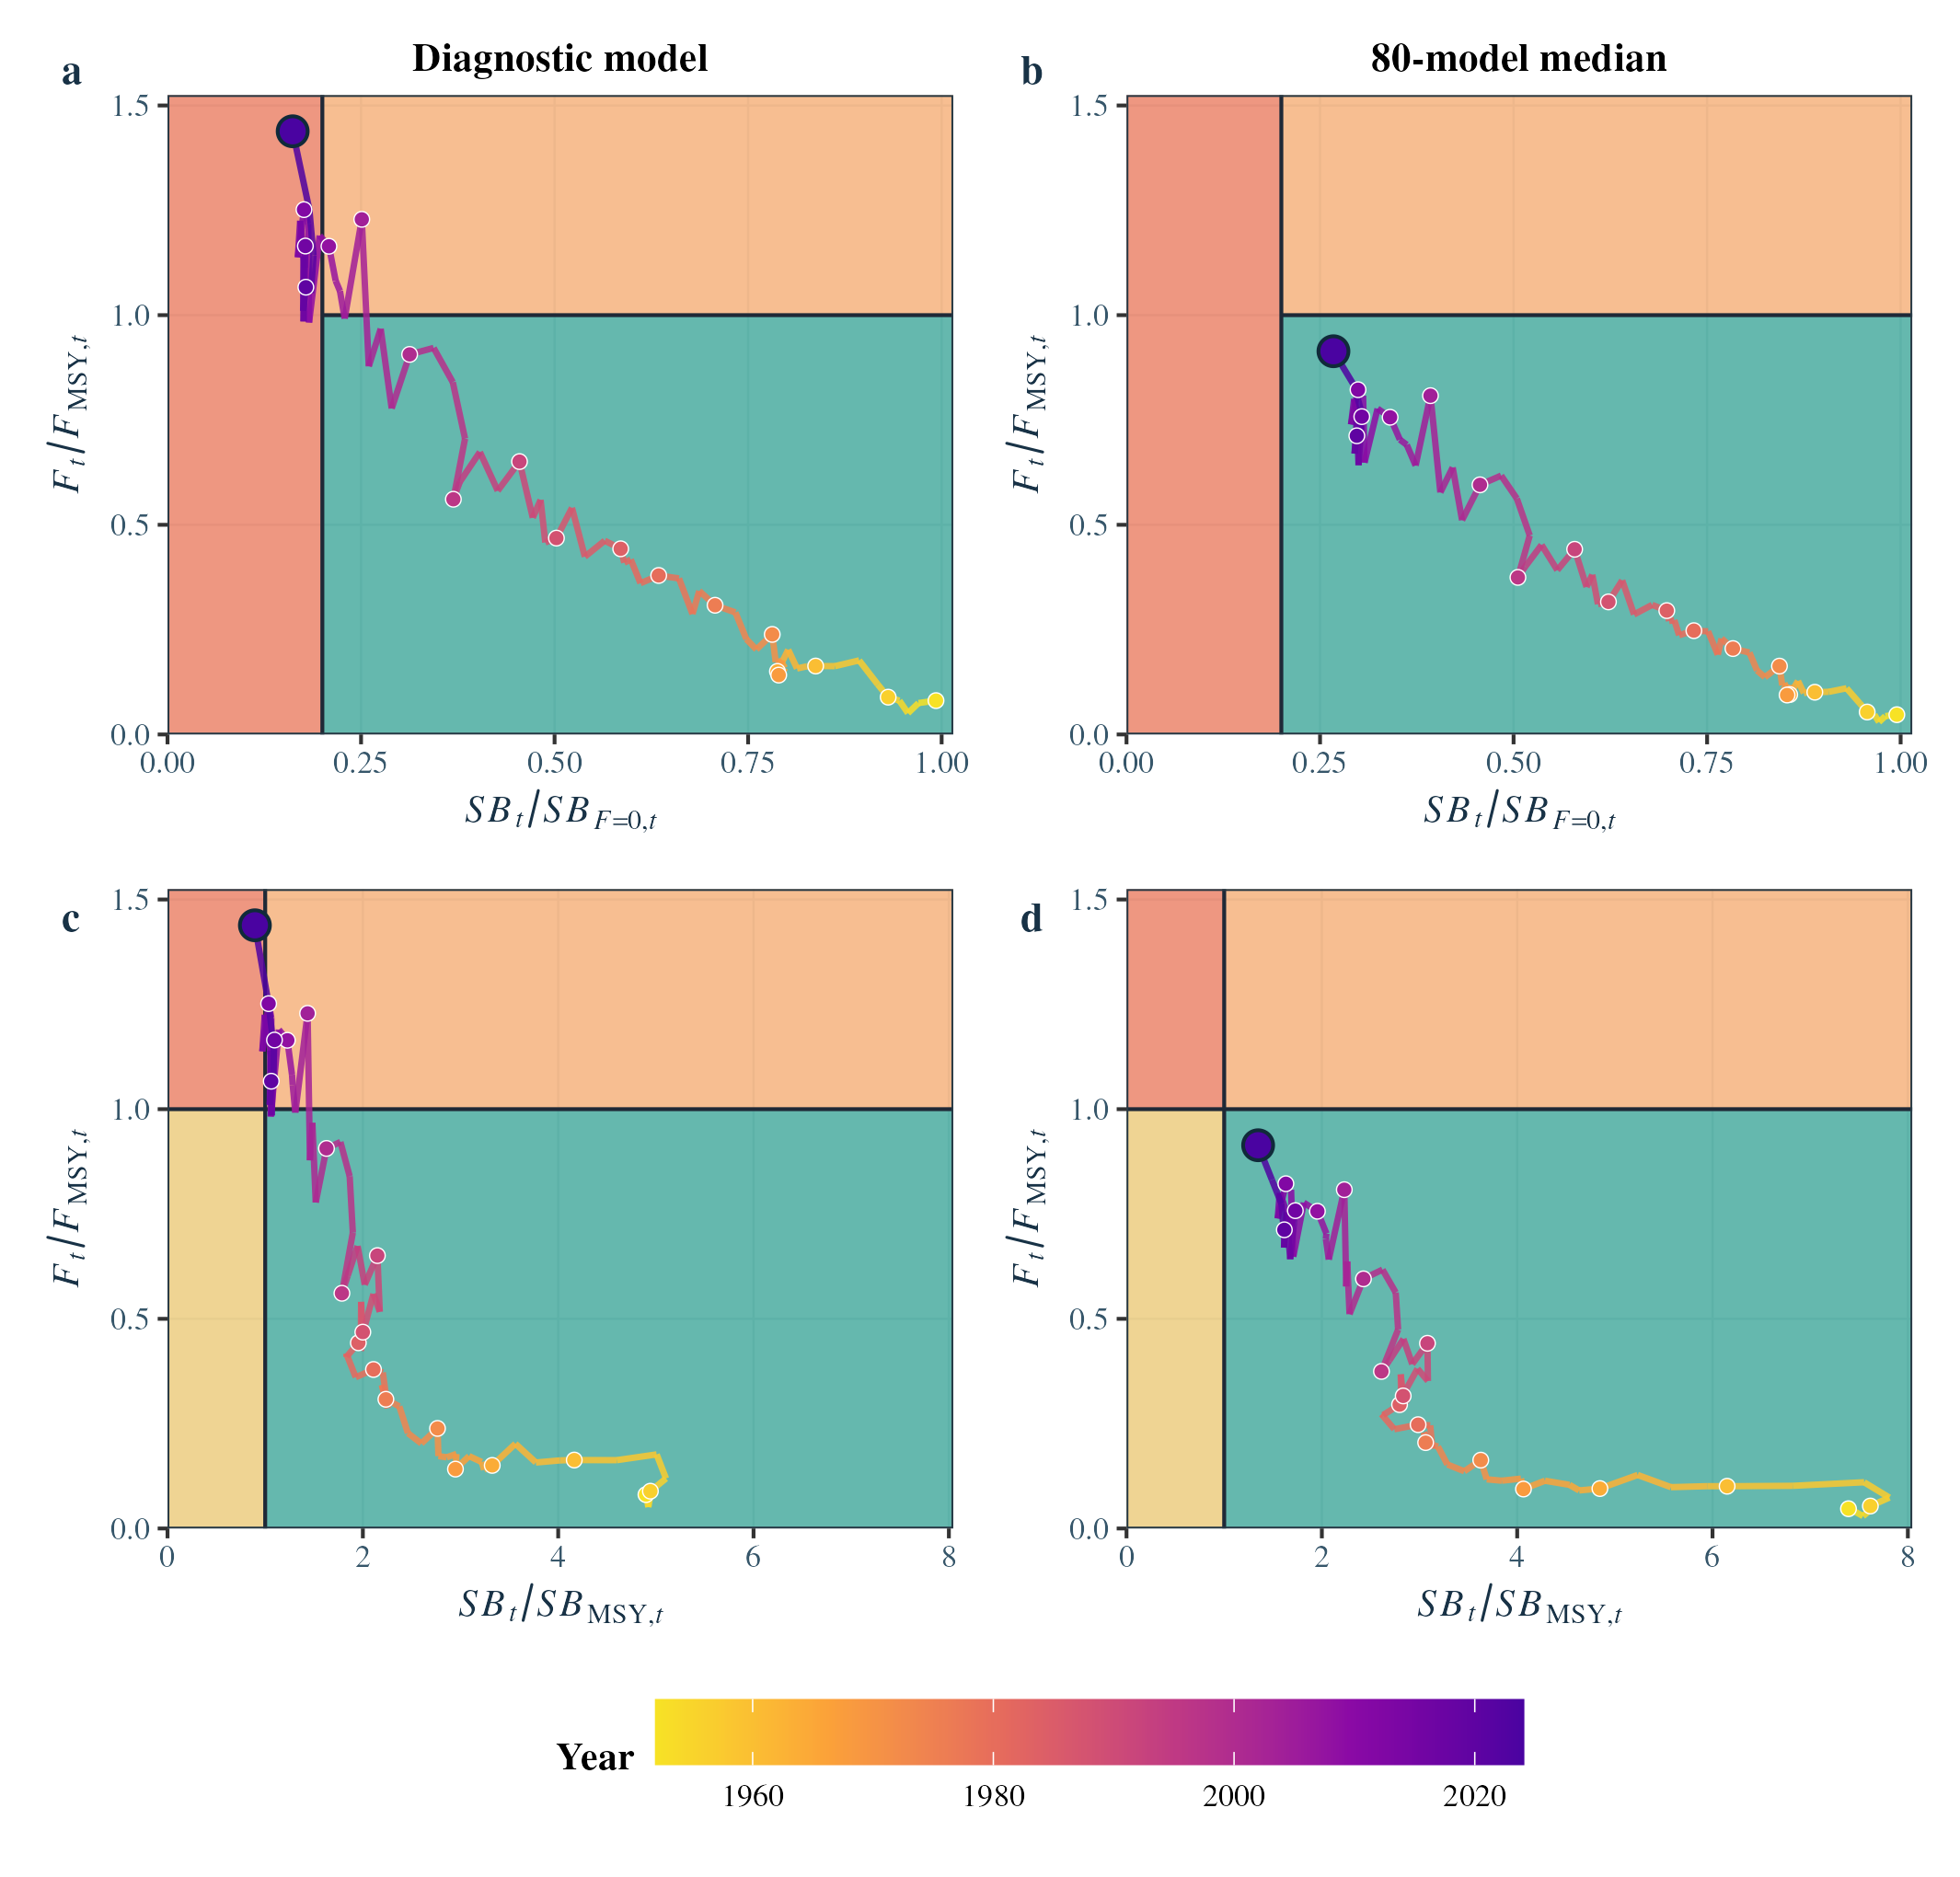
\includegraphics[width=0.8\linewidth,height=\textheight,keepaspectratio]{figures/time-dynamic-kobe-majuro.png}
%DIFDELCMD <

%DIFDELCMD < }
%DIFDELCMD <

%DIFDELCMD < \caption{\label{fig-time-dynamic-kobe-majuro}Time-dynamic Majuro and
%DIFDELCMD < Kobe trajectories for the 2026 diagnostic model and the median of the
%DIFDELCMD < 80-model ensemble. Panels (a) and (b) are Majuro trajectories for the
%DIFDELCMD < diagnostic model and the annual ensemble median, respectively; panels
%DIFDELCMD < (c) and (d) are the corresponding Kobe trajectories. The axes are
%DIFDELCMD < \(SB_{t}\)/\(SB_{F=0}t\) and \(F_{t}\)/\(F_{MSY}t\) for Majuro, and
%DIFDELCMD < \(SB_{t}\)/\(SB_{MSY}t\) and \(F_{t}\)/\(F_{MSY}t\) for Kobe. Colour
%DIFDELCMD < shows year and the outlined point marks 2024. The ensemble trajectory is
%DIFDELCMD < the median of the 80 retained models and therefore represents structural
%DIFDELCMD < medians rather than Hessian estimation uncertainty.}
%DIFDELCMD <

%DIFDELCMD < \end{figure}%%%
\DIFdelend \DIFaddbegin \begin{figure}[H]

\centering{

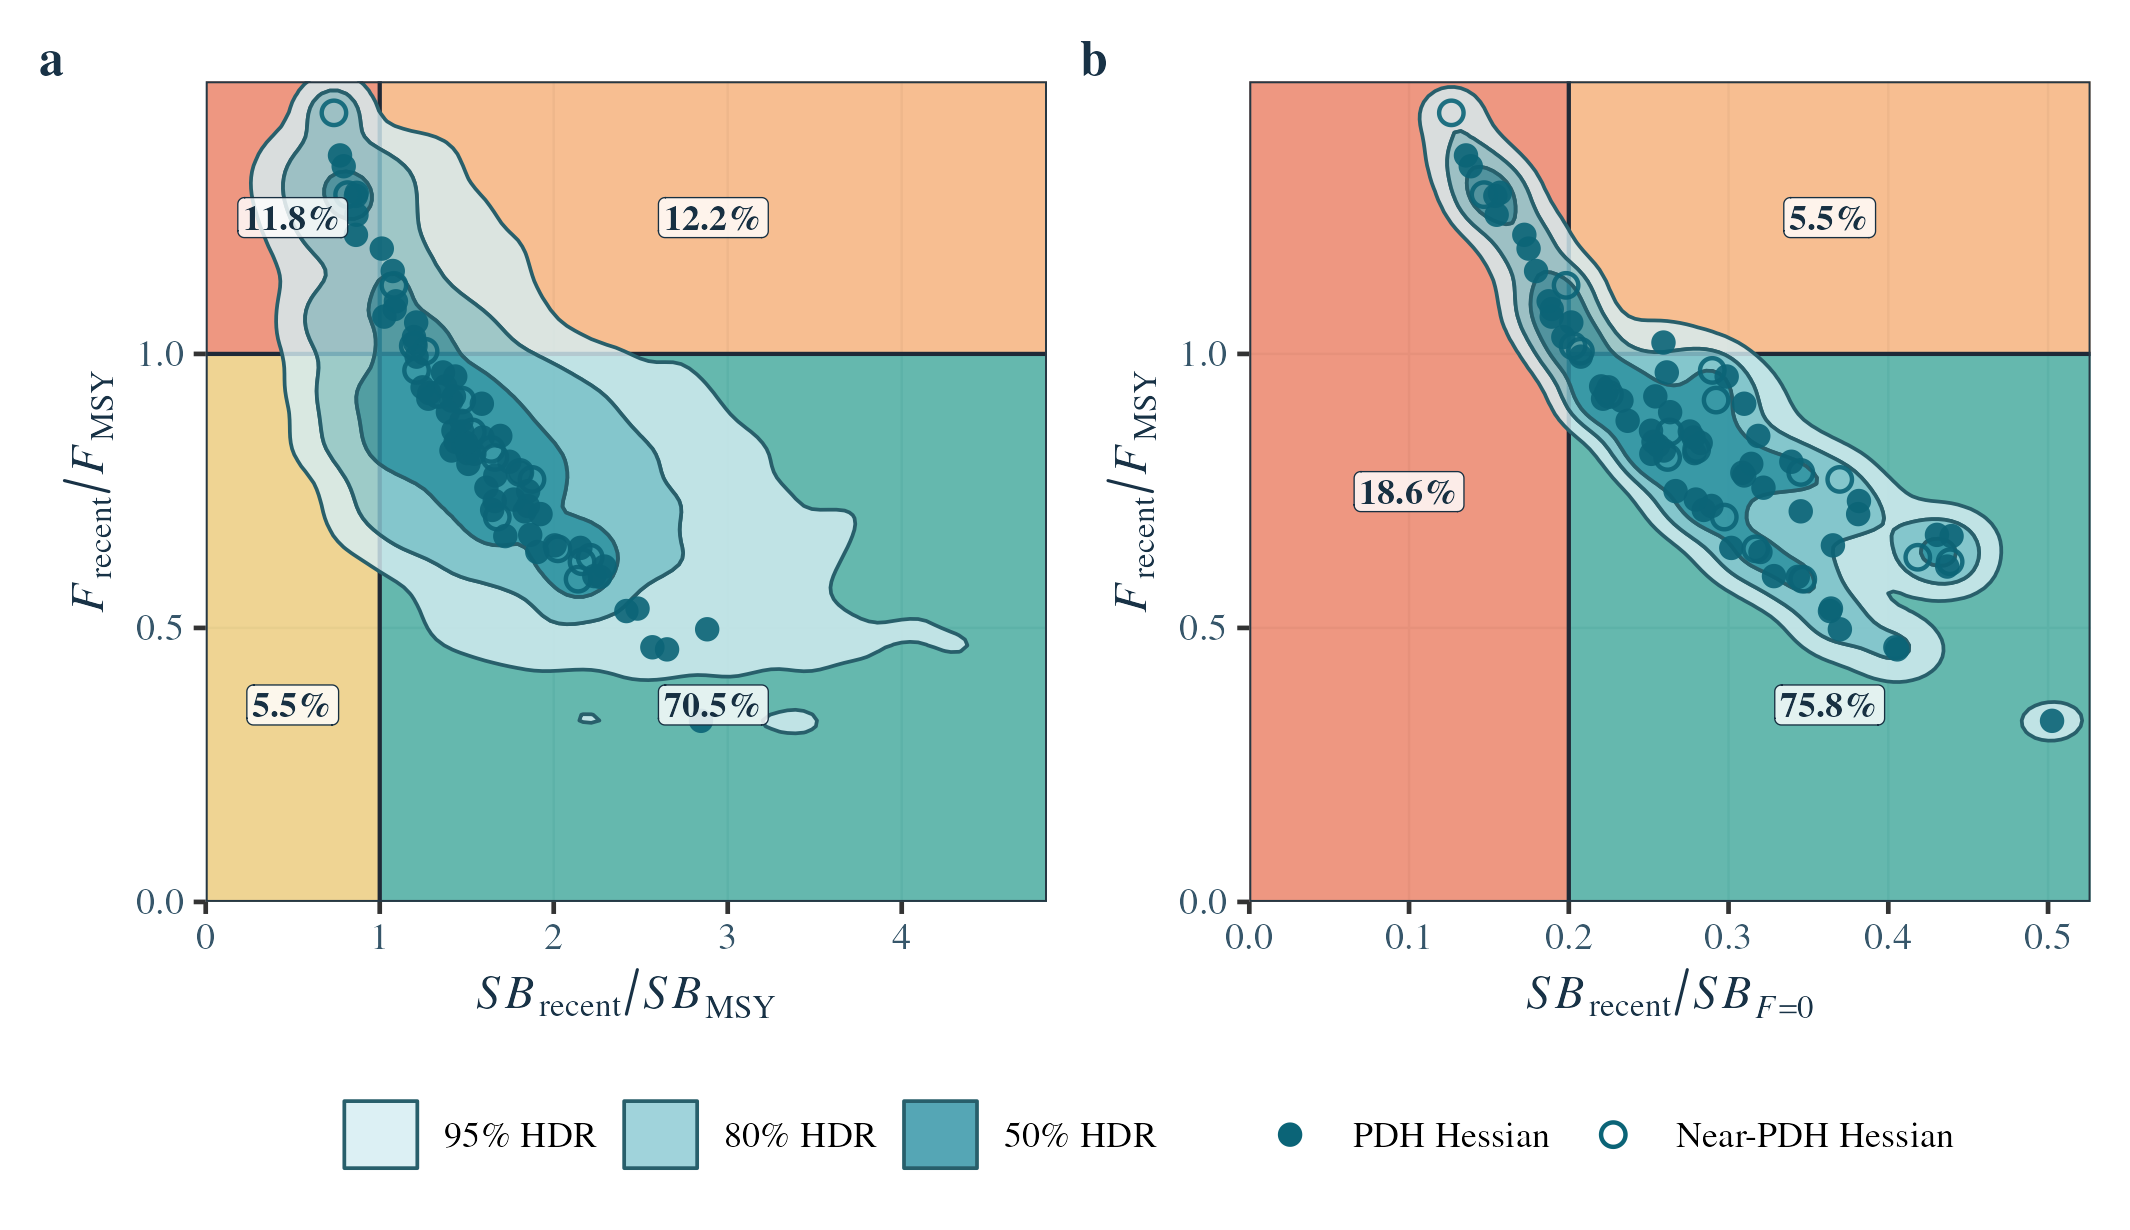
\includegraphics[width=1\linewidth,height=\textheight,keepaspectratio]{figures/combined_kobe_majuro_status.png}

}

\caption{\label{fig-combined-kobe-majuro-status}Stock status based on
\(SB_{recent}\)/\(SB_{F=0}\) (SBrecent 2021--2024) and
\(F_{recent}\)/\(F_{MSY}\) (Frecent 2020--2023). Panel (a) Kobe: is
relative to \(SB_{recent}\)/\(SB_{MSY}\) and \(F_{recent}\)/\(F_{MSY}\)
panel (b) Majuro: \(SB_{recent}\)/\(SB_{F=0}\) and
\(F_{recent}\)/\(F_{MSY}\) with the LRP of \(SB_{recent}\)/\(SB_{F=0}\)
= 0.20. Points are the 80 model estimates; filled and open symbols
distinguish PDH and Near-PDH fits. Nested 50\%, 80\% and 95\% HDRs
combine structural uncertainty with available joint Hessian uncertainty.
Background colours follow the Kobe four-category and Majuro
three-category definitions. Labels give the probability in each category
from the same equal-model-weight distribution used for the combined
HDRs. Open the
\href{https://pacificcommunity.github.io/ofp-sam-bet-2026-ensemble/bet-2026-ensemble-interactive-viewer.html}{interactive
ensemble viewer}.}

\end{figure}%DIF >

\begin{figure}[H]

\centering{

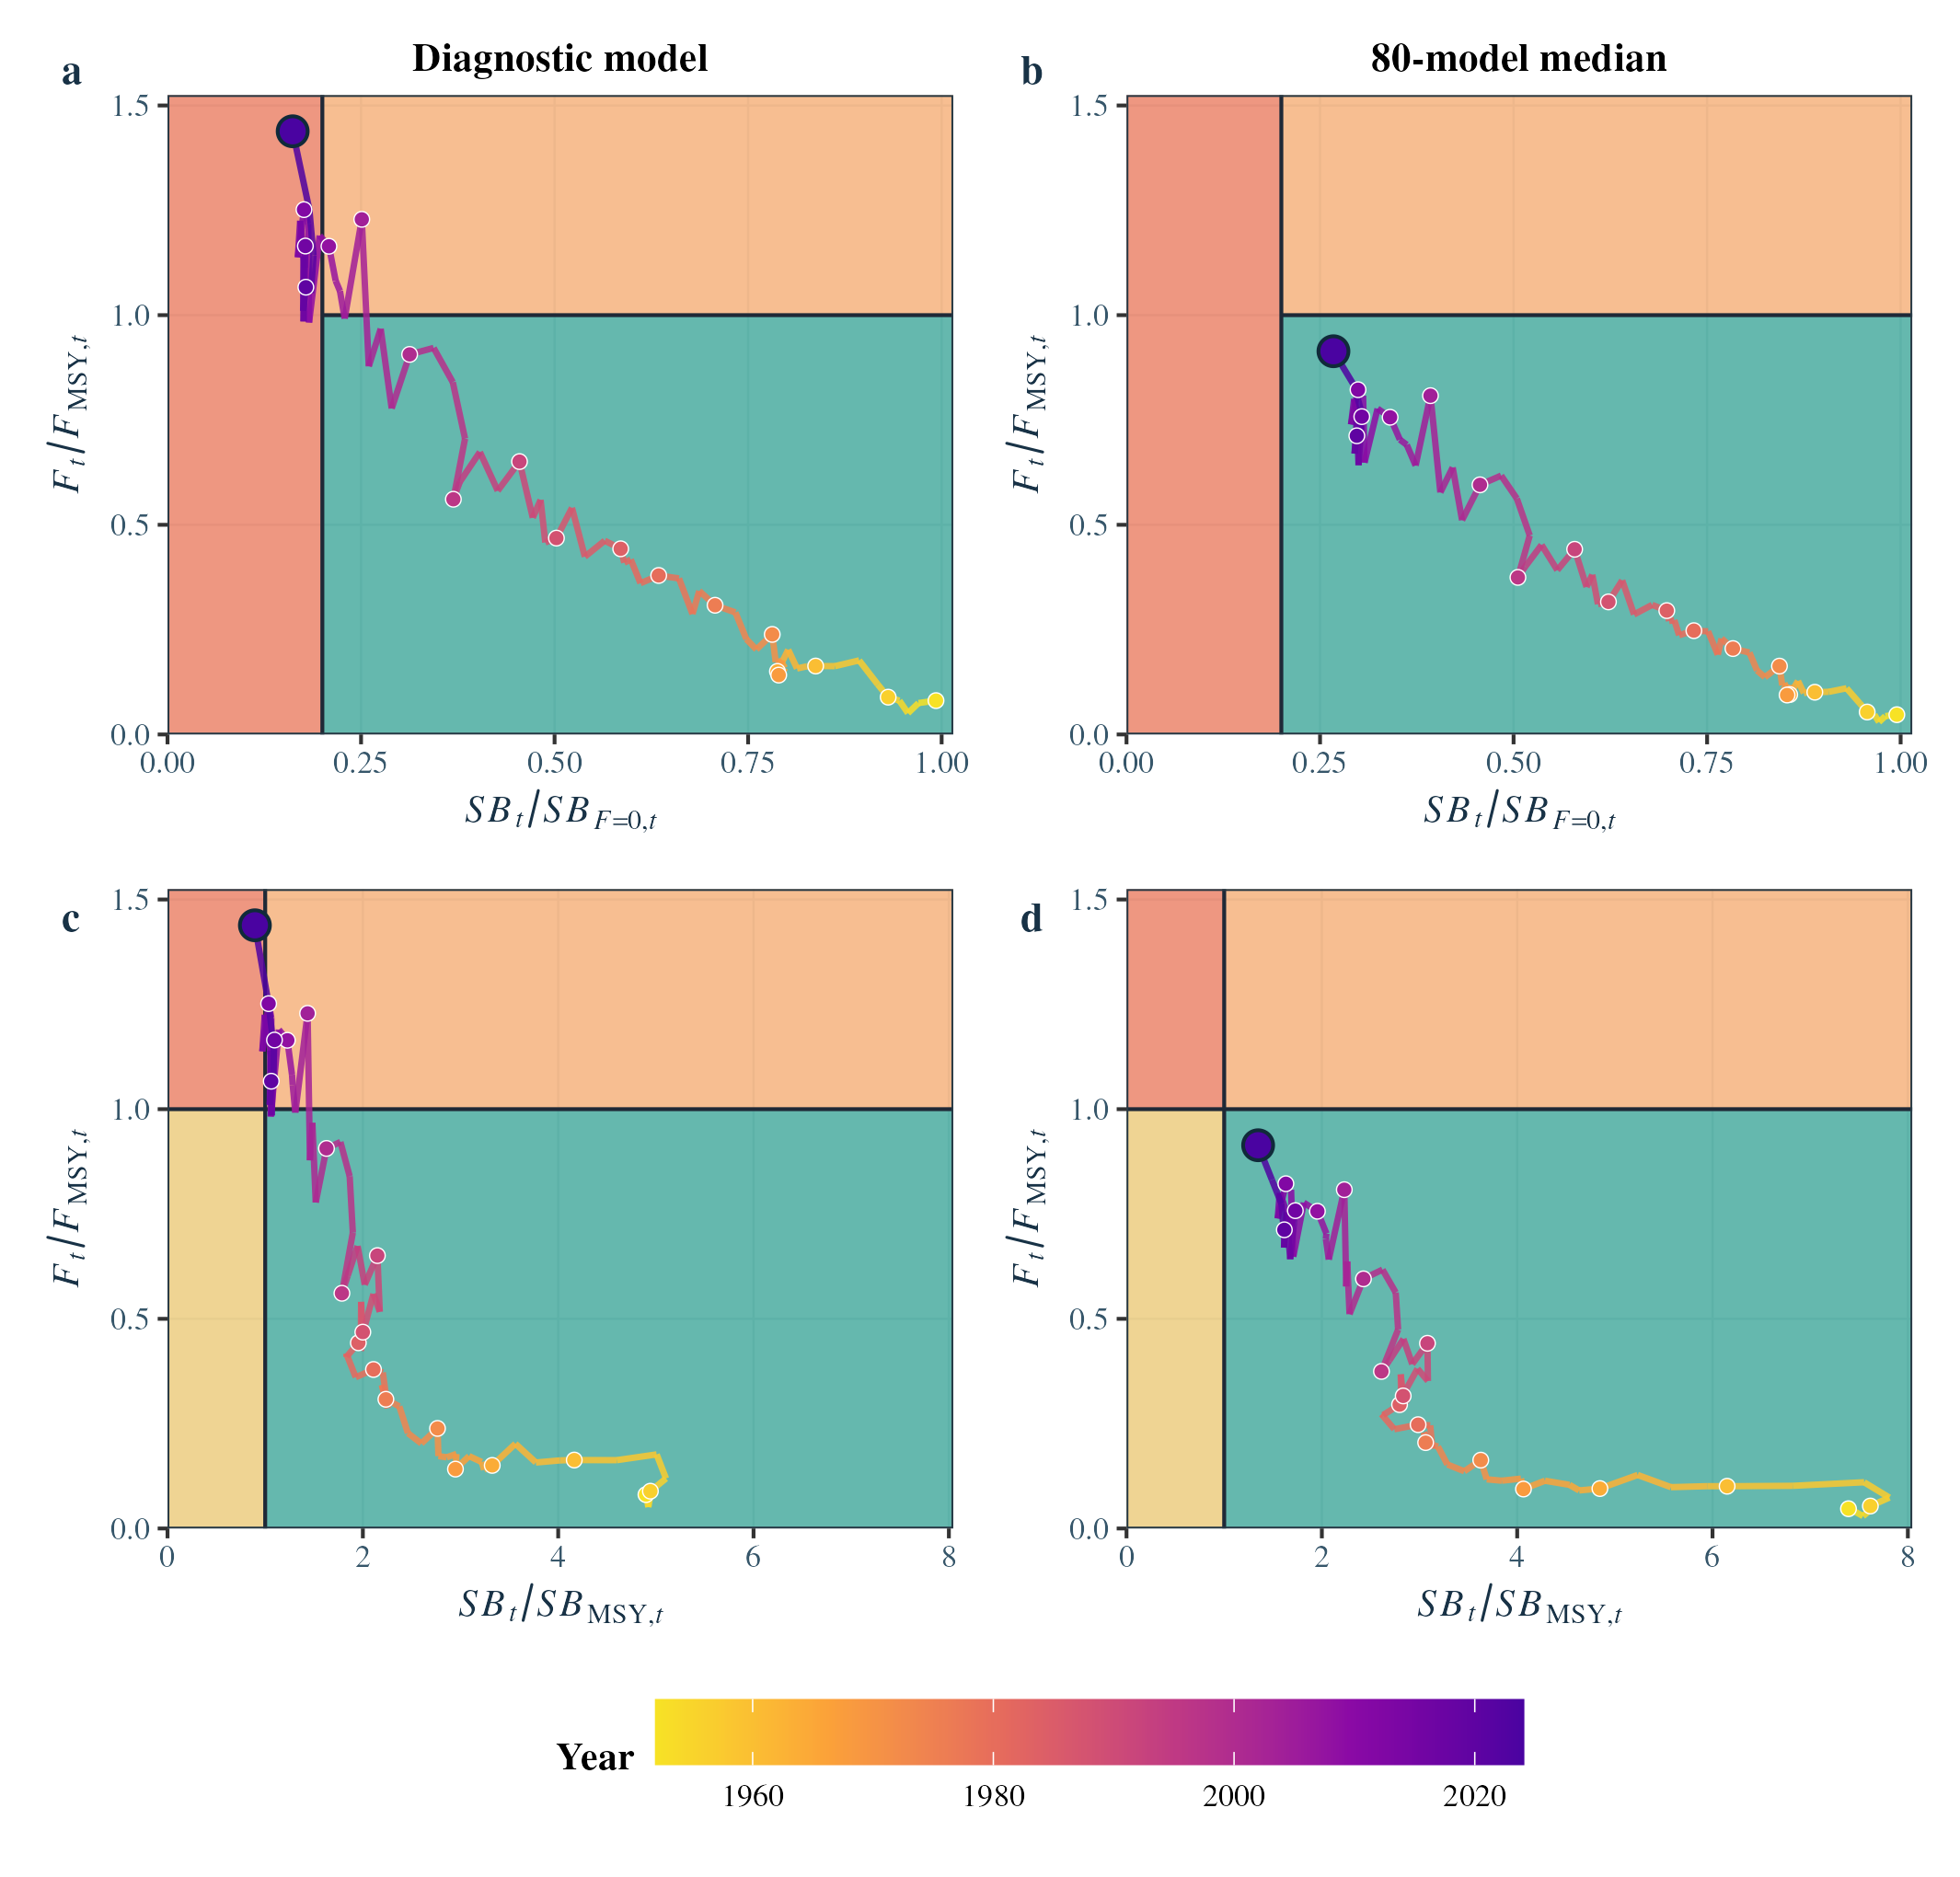
\includegraphics[width=0.8\linewidth,height=\textheight,keepaspectratio]{figures/time-dynamic-kobe-majuro.png}

}

\caption{\label{fig-time-dynamic-kobe-majuro}Time-dynamic Majuro and
Kobe trajectories for the 2026 diagnostic model and the median of the
80-model ensemble. Panels (a) and (b) are Majuro trajectories for the
diagnostic model and the annual ensemble median, respectively; panels
(c) and (d) are the corresponding Kobe trajectories. The axes are
\(SB_{t}\)/\(SB_{F=0}t\) and \(F_{t}\)/\(F_{MSY}t\) for Majuro, and
\(SB_{t}\)/\(SB_{MSY}t\) and \(F_{t}\)/\(F_{MSY}t\) for Kobe. Colour
shows year and the outlined point marks 2024. The ensemble trajectory is
the median of the 80 retained models and therefore represents structural
medians rather than Hessian estimation uncertainty. Open the
\href{https://pacificcommunity.github.io/ofp-sam-bet-2026-ensemble/bet-2026-ensemble-interactive-viewer.html}{interactive
ensemble viewer}.}

\end{figure}\DIFaddend %

\begin{figure}[H]

\centering{

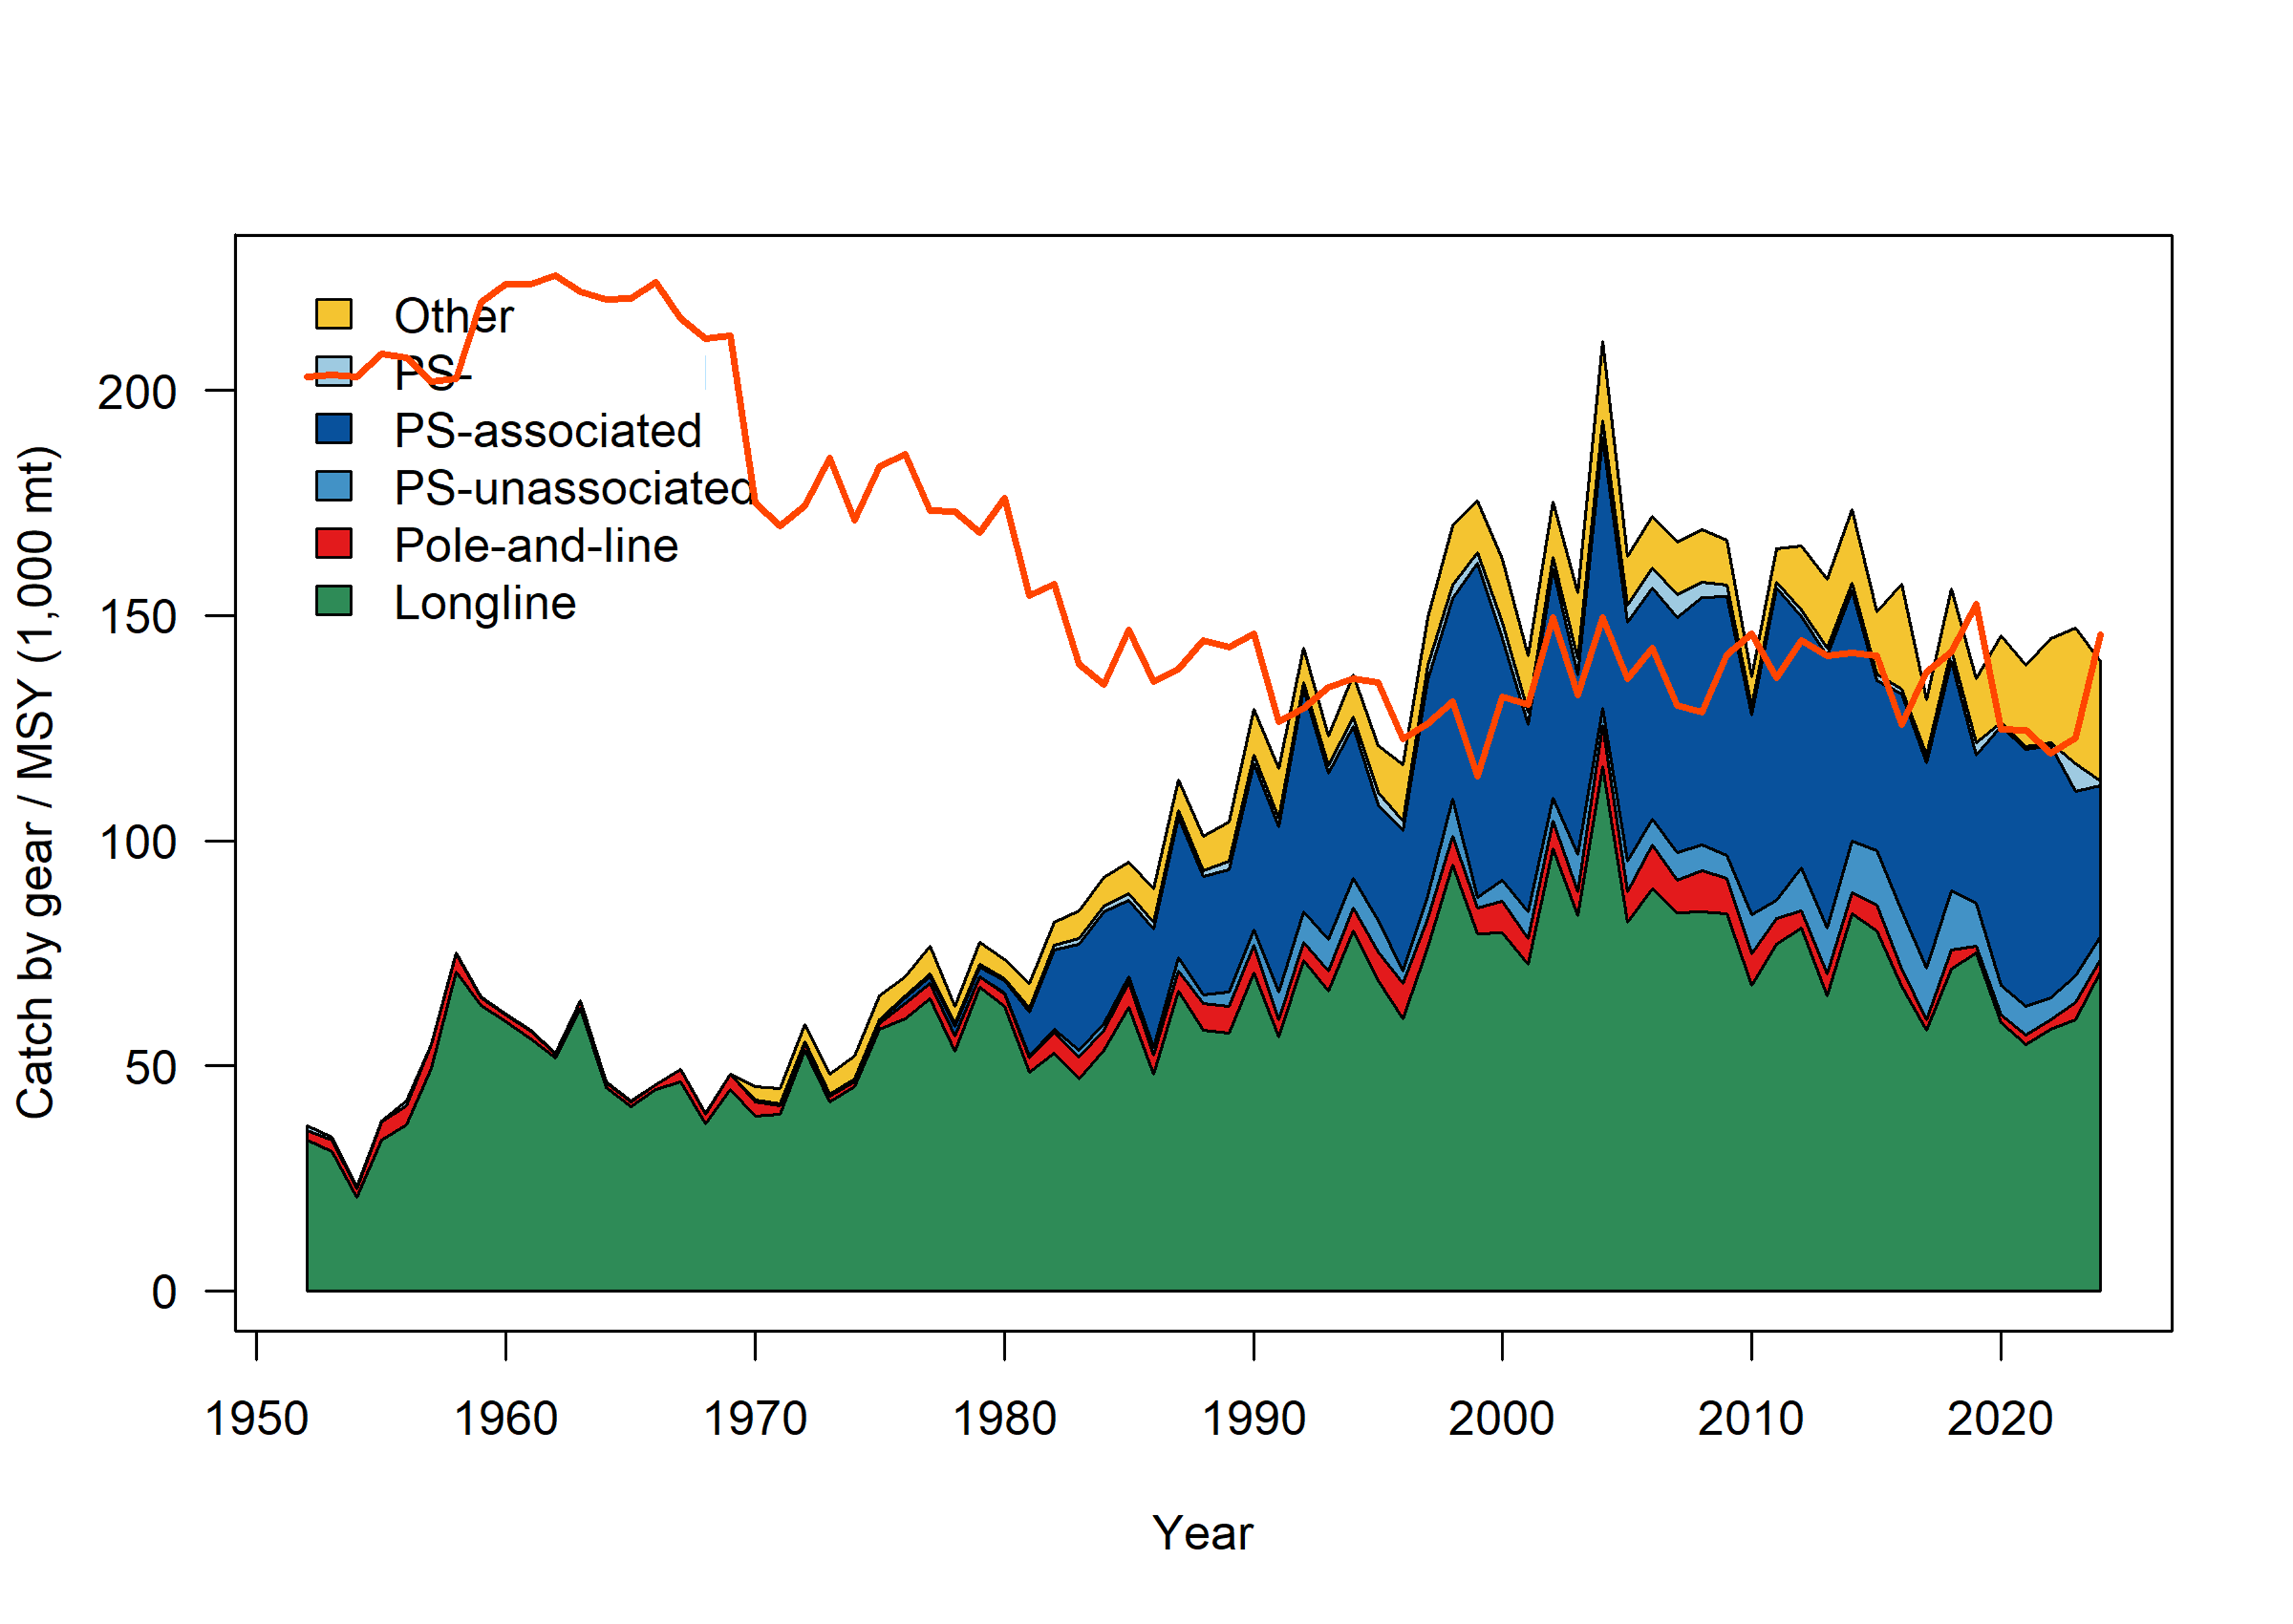
\includegraphics[width=1\linewidth,height=\textheight,keepaspectratio]{figures/dynamic_msy.png}

}

\caption{\label{fig-dynamic-msy}History of the annual estimates of MSY
(red line) for the diagnostic model compared with annual catch by the
main gear types. Note that this is a `dynamic' MSY.}

\end{figure}%

\DIFdelbegin %DIFDELCMD < \begin{figure}[H]
%DIFDELCMD <

%DIFDELCMD < \centering{
%DIFDELCMD <

%DIFDELCMD < 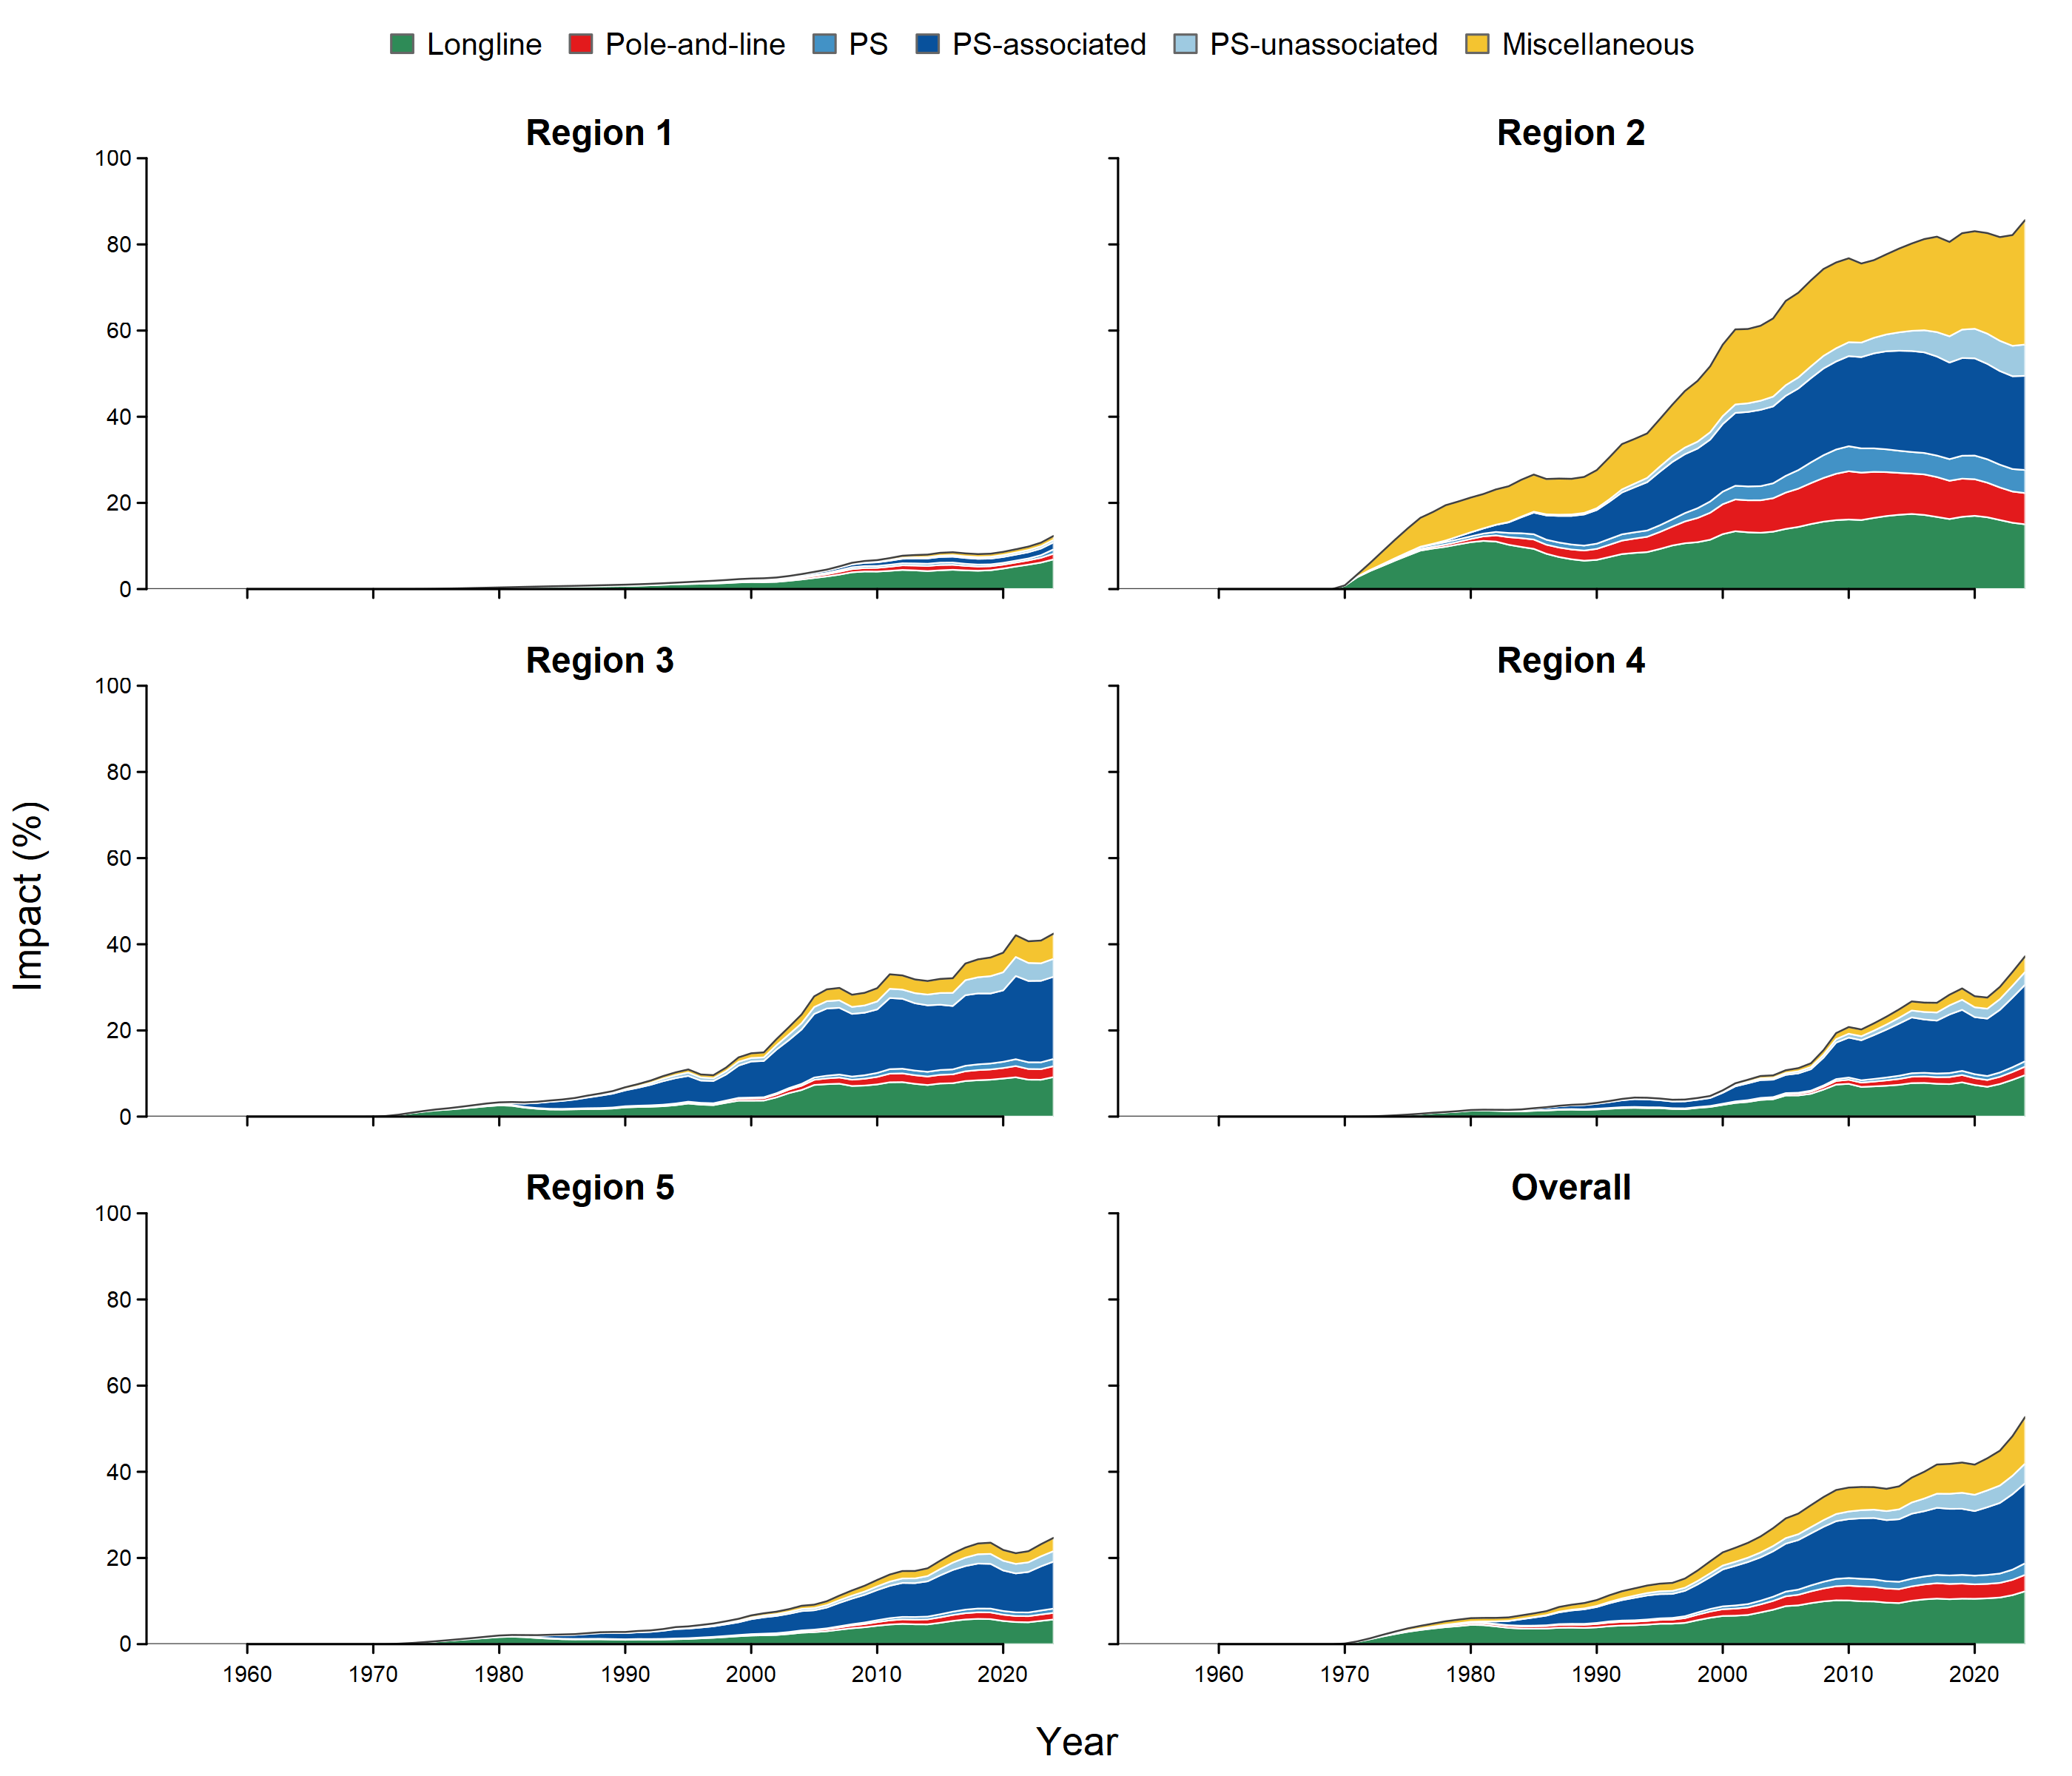
\includegraphics[width=1\linewidth,height=\textheight,keepaspectratio]{figures/impact_region.png}
%DIFDELCMD <

%DIFDELCMD < }
%DIFDELCMD <

%DIFDELCMD < \caption{\label{fig-impact-region}Estimates of fishery impact, or
%DIFDELCMD < reduction in spawning potential due to fishing (Fishery Impact =
%DIFDELCMD < \(1-SB_{t}/SB_{t,F=0}\)) by region, and over all regions (bottom right),
%DIFDELCMD < attributed to various fishery groups for the 2023 diagnostic model.}
%DIFDELCMD <

%DIFDELCMD < \end{figure}%%%
\DIFdelend \DIFaddbegin \begin{figure}[H]

\centering{

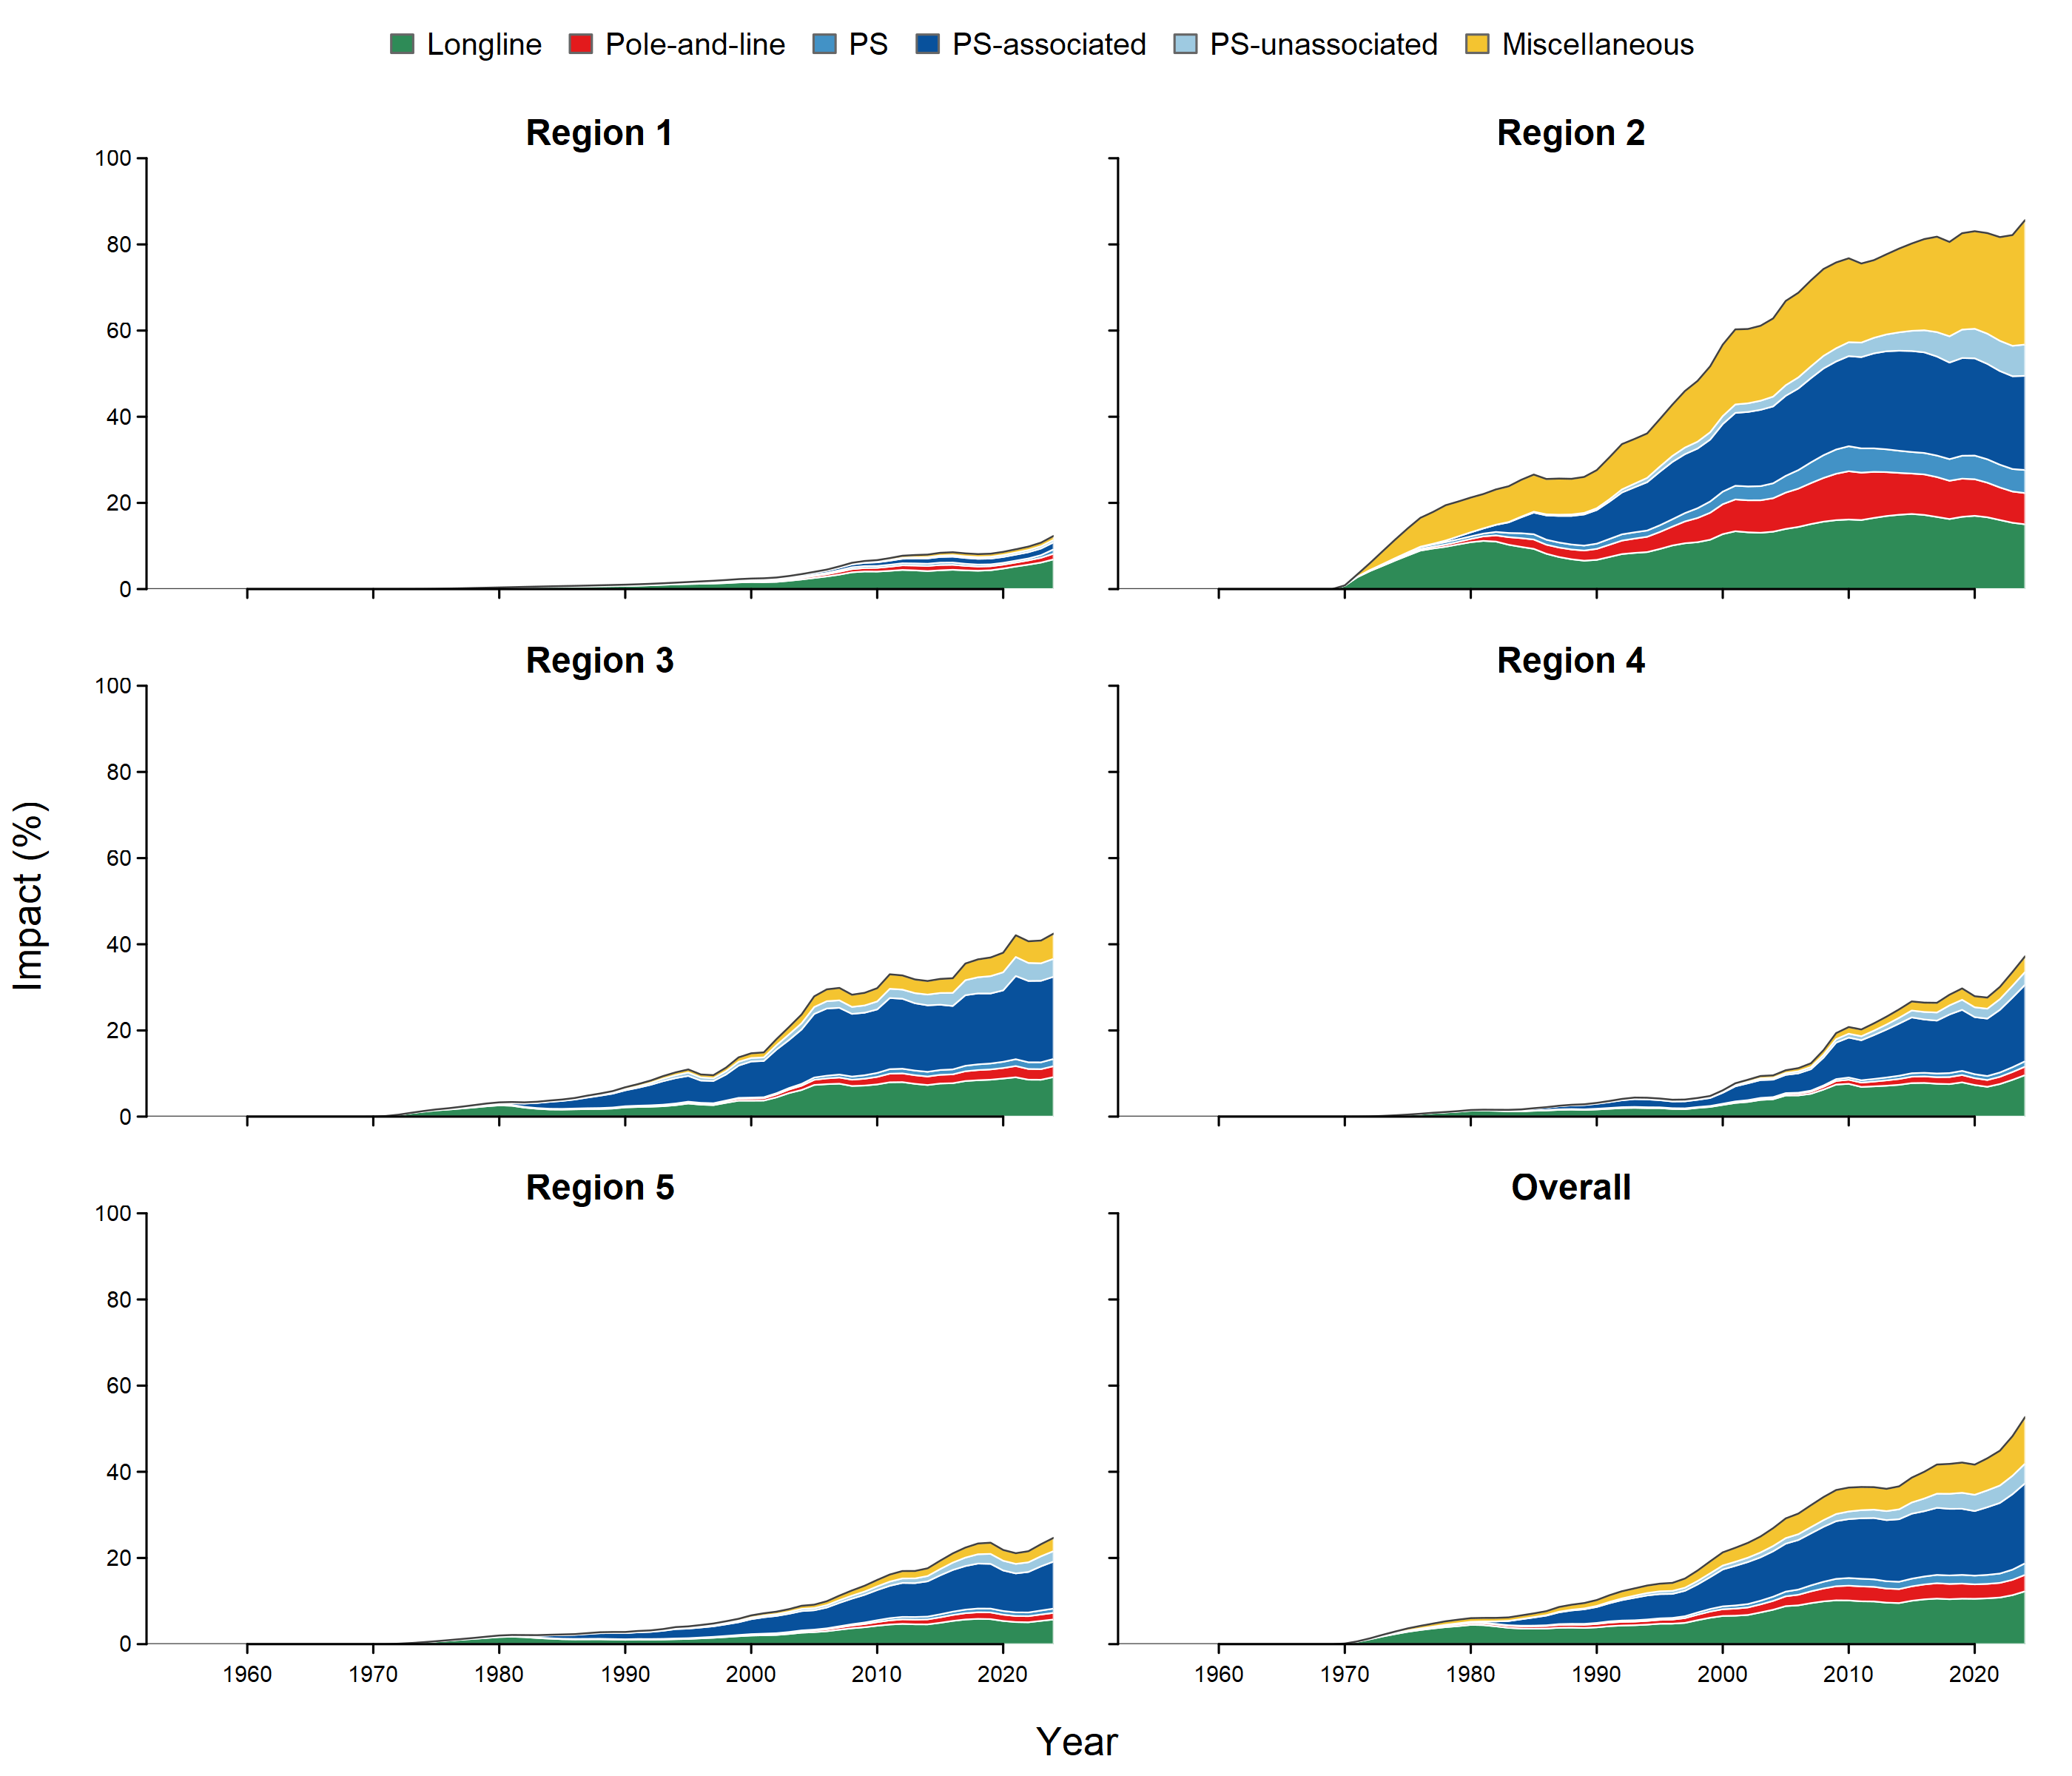
\includegraphics[width=1\linewidth,height=\textheight,keepaspectratio]{figures/impact_region.png}

}

\caption{\label{fig-impact-region}Estimates of fishery impact, or
reduction in spawning potential due to fishing (fishery impact =
\(1-SB_{t}/SB_{t,F=0}\)), by region and over all regions (bottom right),
attributed to fishery groups for the 2026 diagnostic model.}

\end{figure}\DIFaddend %

\begin{figure}[H]

\centering{

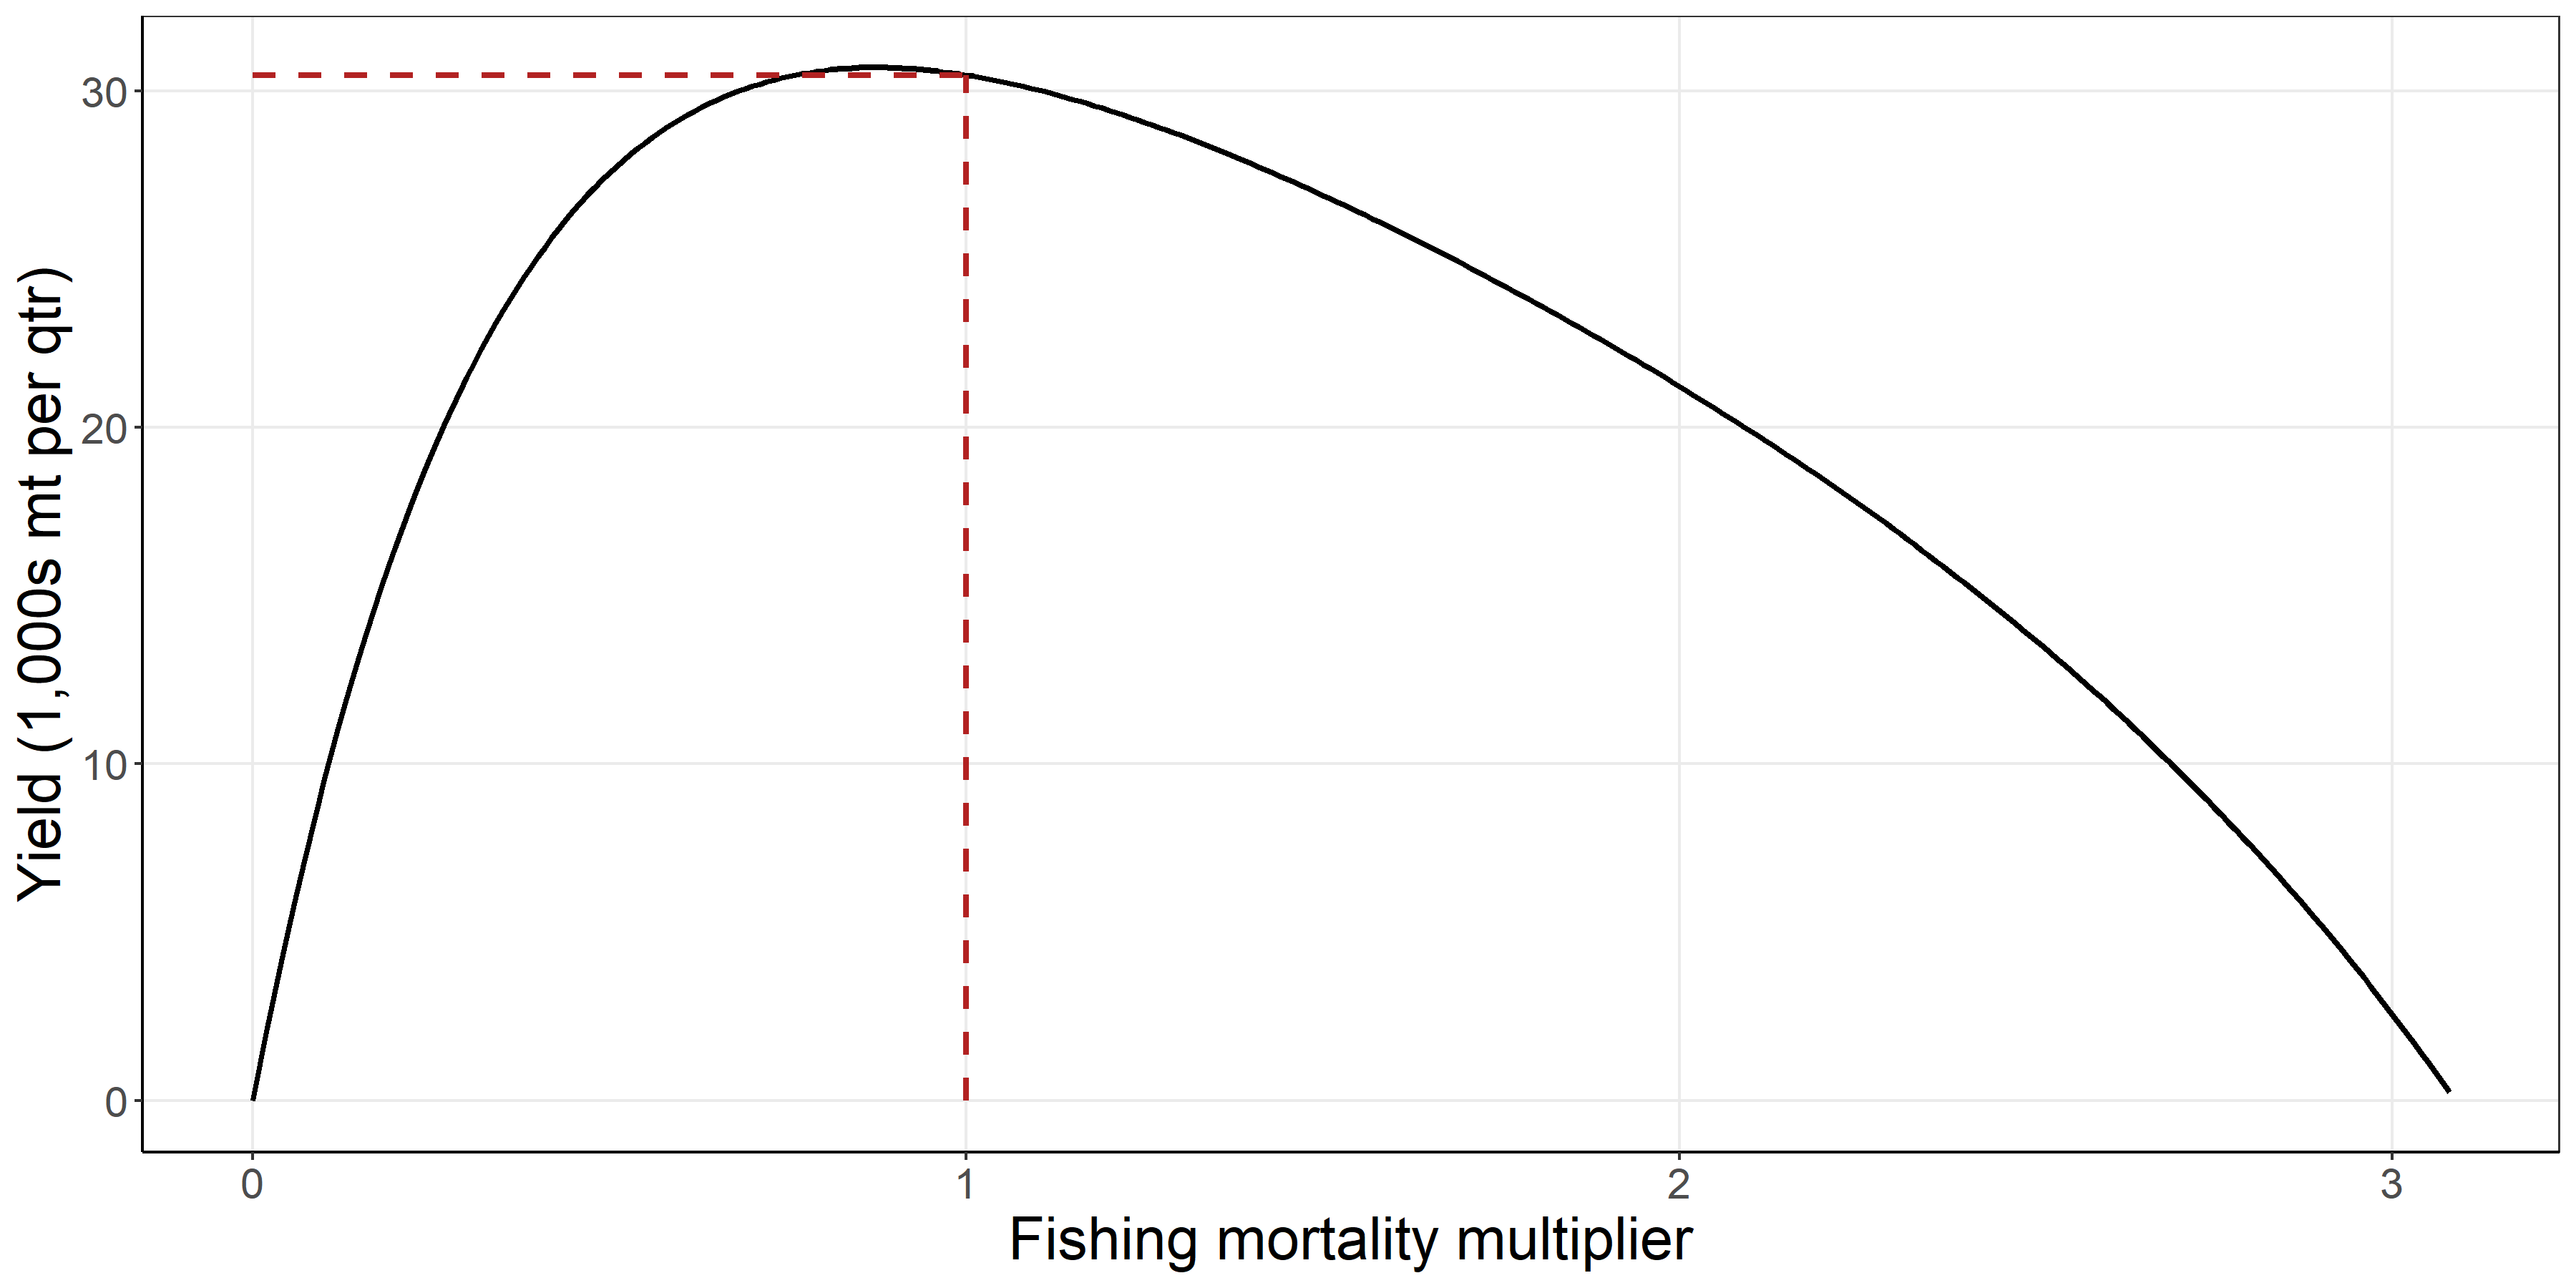
\includegraphics[width=1\linewidth,height=\textheight,keepaspectratio]{figures/yield.png}

}

\caption{\label{fig-yield}Estimated yield as a function of fishing
mortality multiplier for the diagnostic model and the alternative mixing
scenario model. The black dashed line indicates the equilibrium yield at
current fishing mortality.}

\end{figure}%

\DIFdelbegin %DIFDELCMD < \begin{figure}[H]
%DIFDELCMD <

%DIFDELCMD < \centering{
%DIFDELCMD <

%DIFDELCMD < 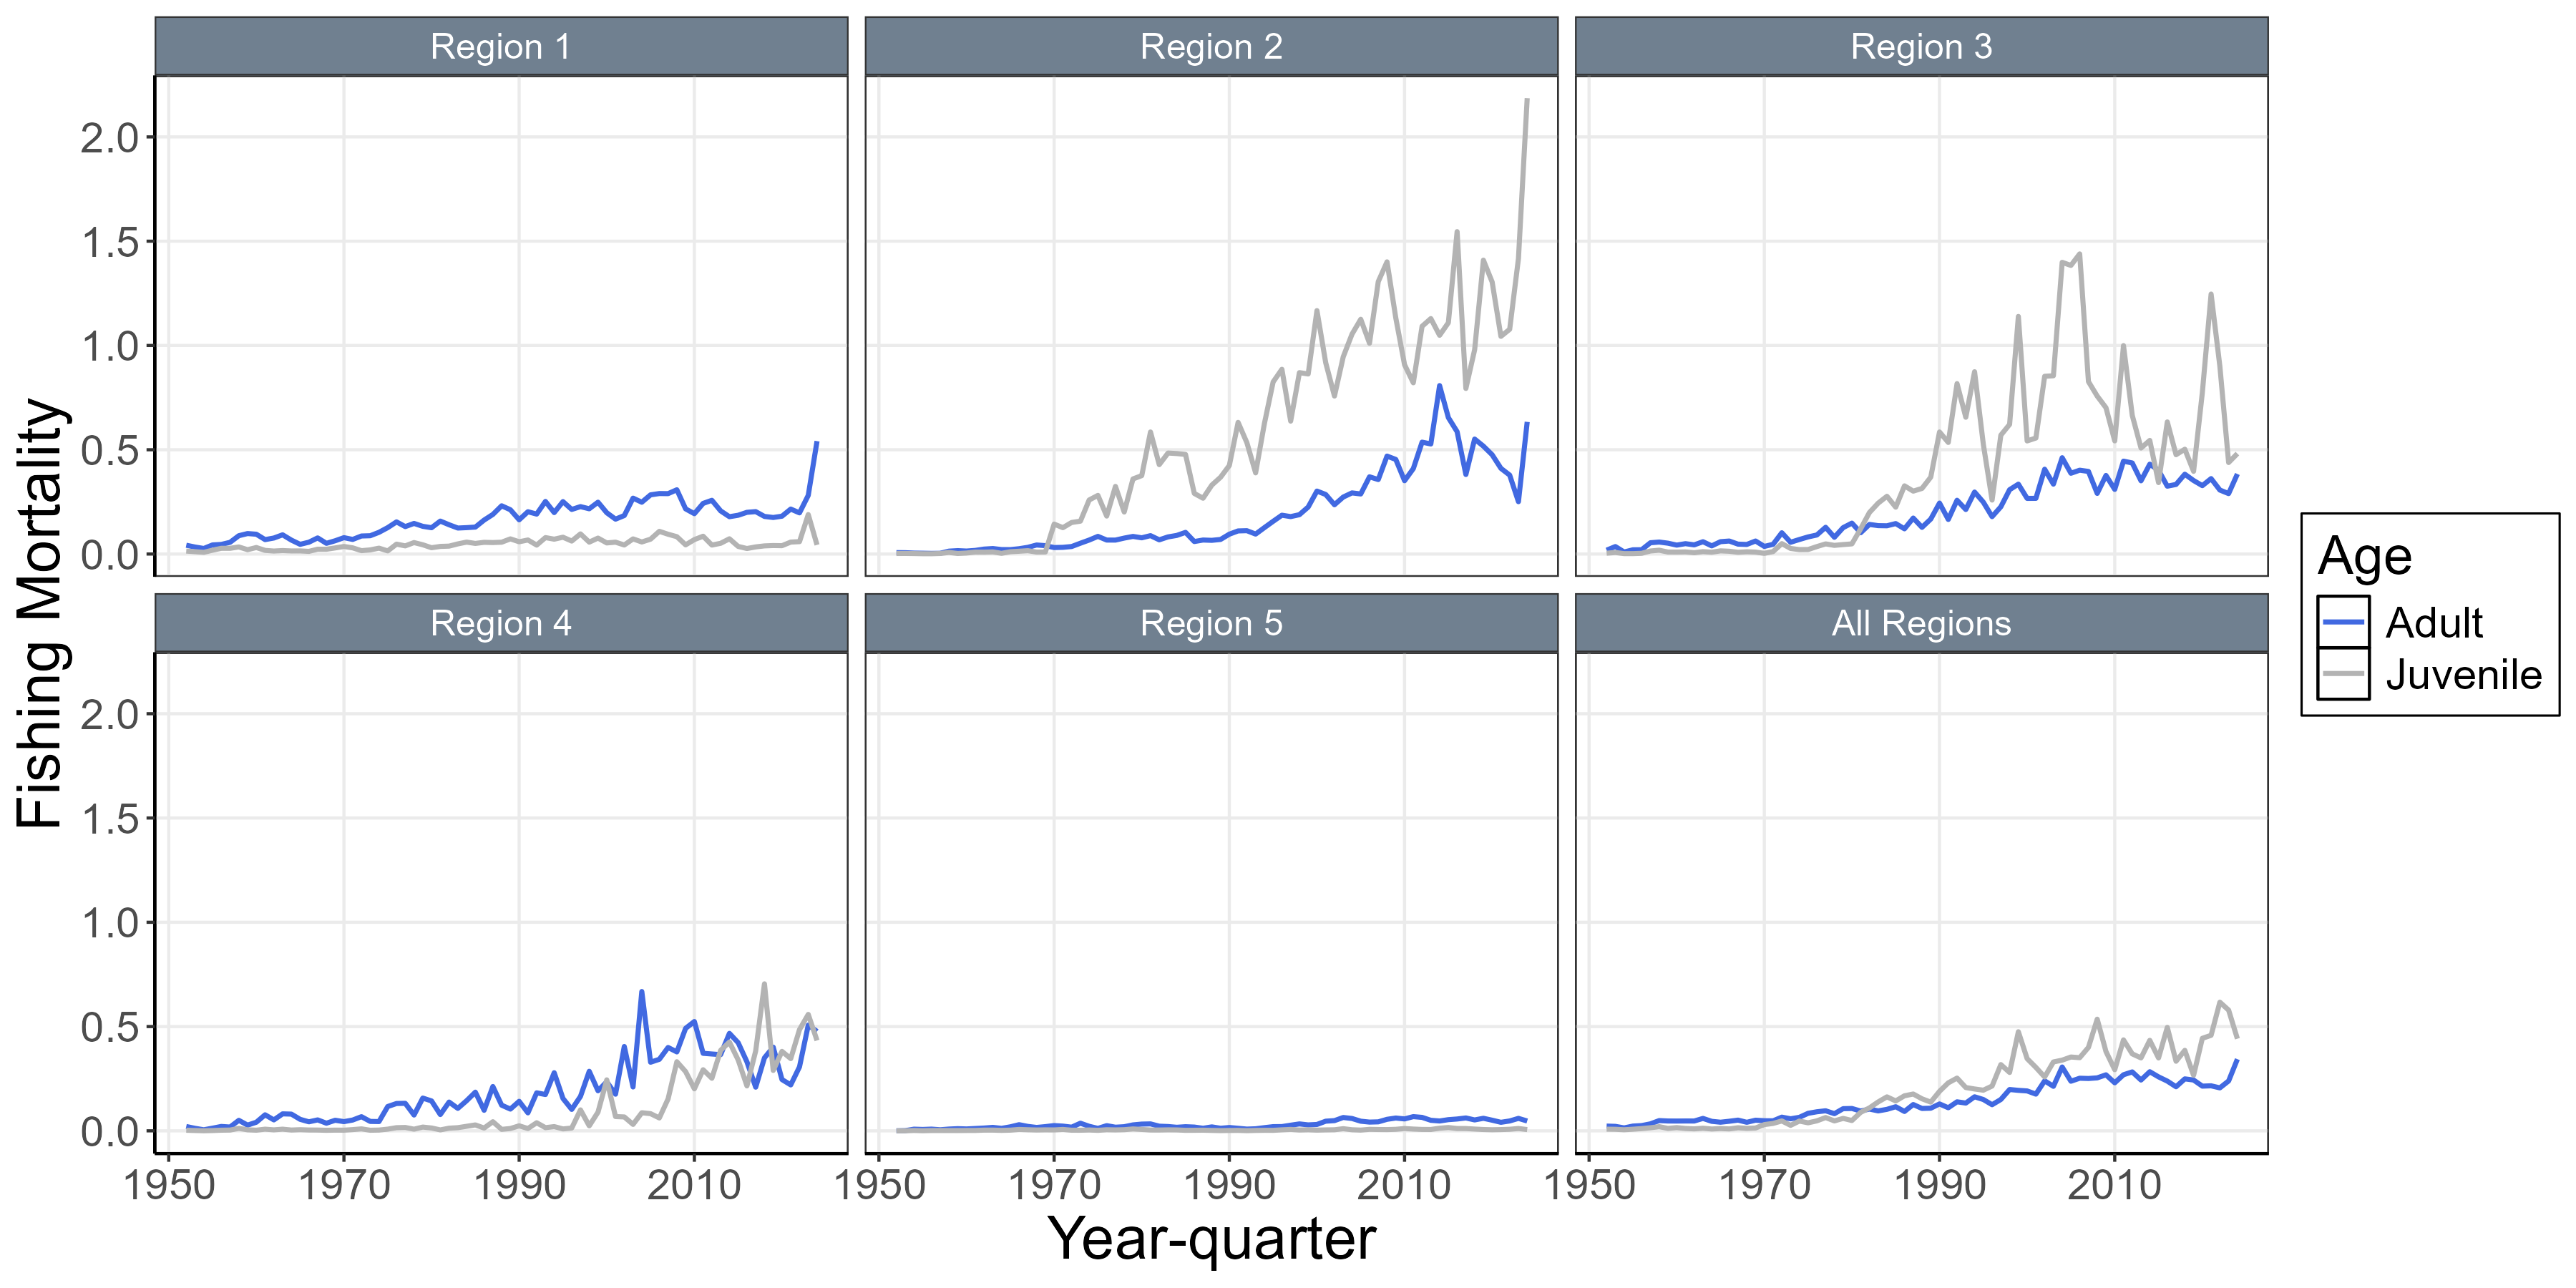
\includegraphics[width=1\linewidth,height=\textheight,keepaspectratio]{figures/F_adult_juv_regions.png}
%DIFDELCMD <

%DIFDELCMD < }
%DIFDELCMD <

%DIFDELCMD < \caption{\label{fig-juv-adult-F}Annual juvenile and adult fishing
%DIFDELCMD < mortality by region and for all regions.}
%DIFDELCMD <

%DIFDELCMD < \end{figure}%%%
\DIFdelend \DIFaddbegin \begin{figure}[H]

\centering{

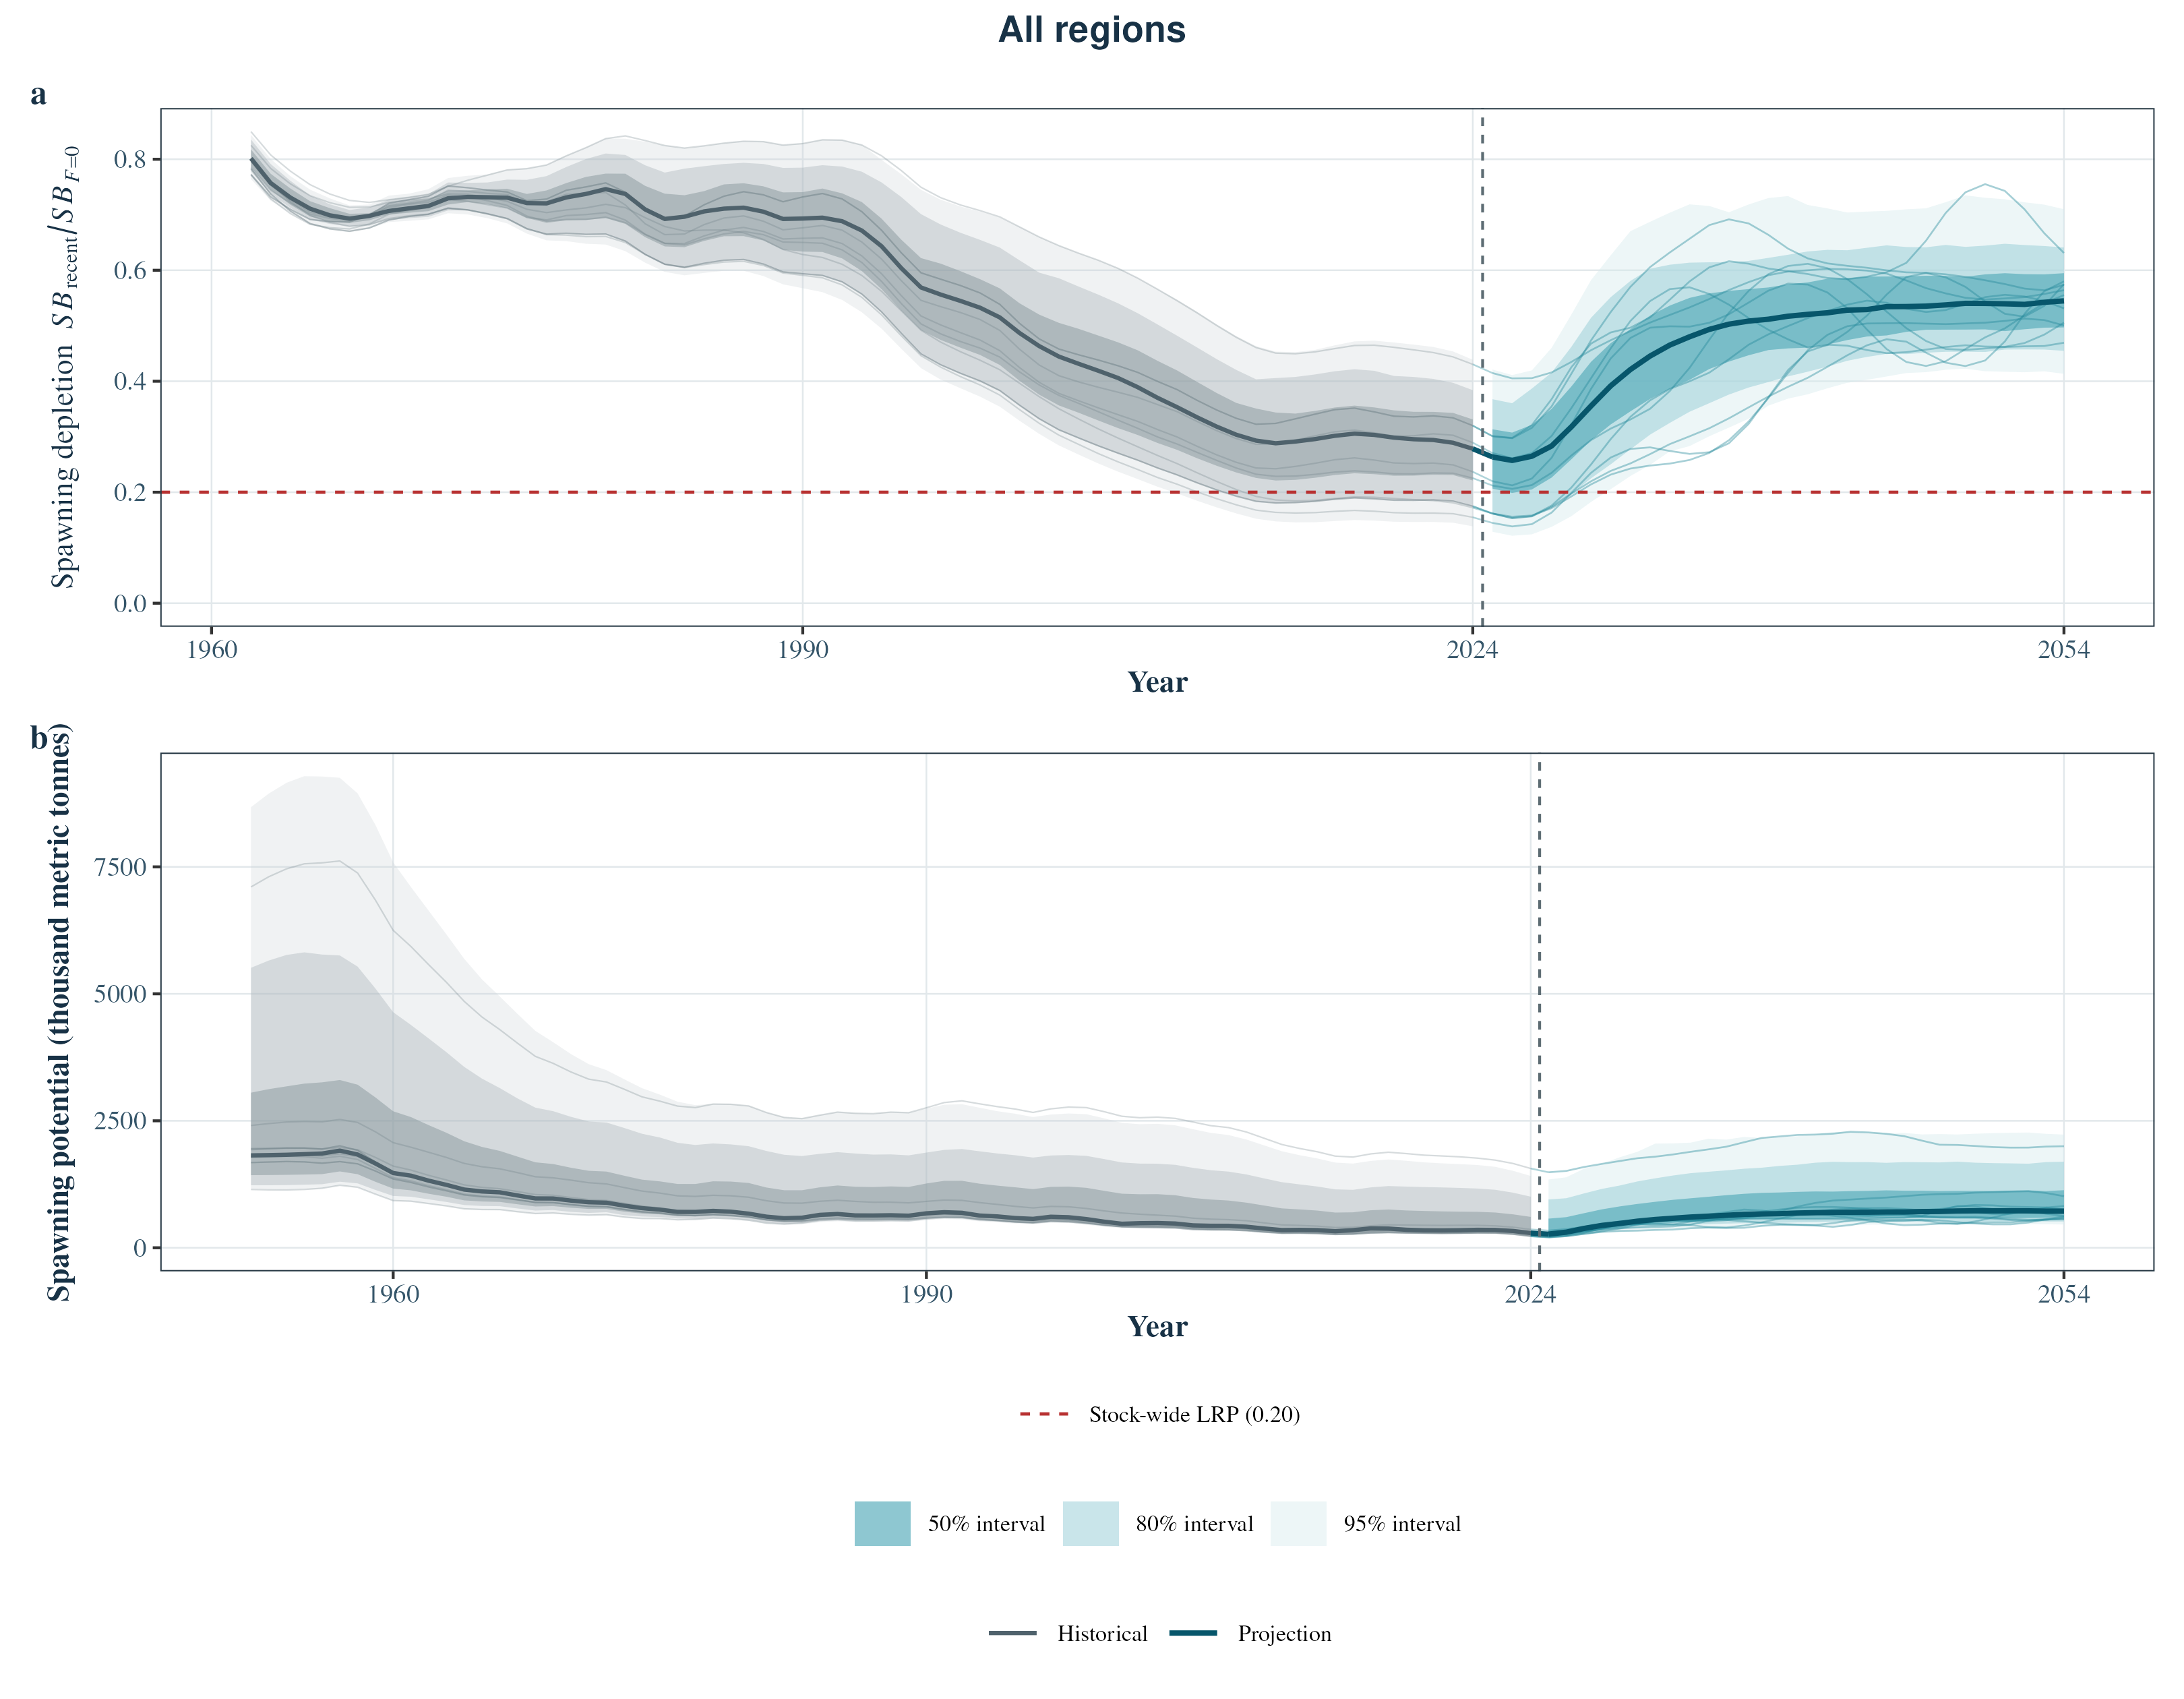
\includegraphics[width=1\linewidth,height=\textheight,keepaspectratio]{figures_new/projection-stock-trajectories.png}

}

\caption{\label{fig-projection-stock-trajectories}All-region spawning
depletion (a) and spawning potential in thousand metric tonnes (b),
joining estimates through 2024 to projections for 2025--2054. Depletion
is the four-year mean spawning biomass divided by the preceding ten-year
mean no-fishing biomass. Medians and central 50\%, 80\% and 95\%
intervals use all 800 model--recruitment realisations; ten thin lines
show individual projection realisations. Historical intervals show
structural uncertainty; projections add recruitment variability without
Hessian parameter draws. The 0.20 line in panel a is the stock-wide LRP.
Open the
\href{https://pacificcommunity.github.io/ofp-sam-bet-2026-ensemble/bet-2026-ensemble-interactive-viewer.html}{interactive
ensemble viewer}.}

\end{figure}\DIFaddend %

\DIFaddbegin \appendix
\setcounter{figure}{0}
\renewcommand{\thefigure}{A\arabic{figure}}
\setcounter{table}{0}
\renewcommand{\thetable}{A\arabic{table}}

\DIFaddend \section{Appendices}\label{sec-appendices}

\DIFdelbegin \DIFdel{Likely to be added
}\DIFdelend \DIFaddbegin \subsection{\DIFadd{Interactive supporting
resources}}\label{sec-interactive-resources}

\DIFadd{The following self-contained browser reports provide selectable model
detail that cannot be reproduced legibly in the static figures. All
links were checked during preparation of Revision 1. The PDF figures and
tables remain the publication record; the viewers are supporting
exploration tools.
}

\begin{itemize}
\item
  \href{https://pacificcommunity.github.io/ofp-sam-bet-2026-stepwise/interactive-model-viewer.html}{\DIFadd{Stepwise
  model-development viewer}}\DIFadd{: comparison of the 2023 refit, intermediate
  development steps and the 2026 diagnostic model.
}\item
  \href{https://pacificcommunity.github.io/ofp-sam-bet-2026-diagnostic/bet-2026-diagnostic-report.html}{\DIFadd{Diagnostic
  report}}\DIFadd{: model-fit, population-dynamics, diagnostic and configuration
  outputs, including downloadable tables.
}\item
  \href{https://pacificcommunity.github.io/ofp-sam-bet-2026-diagnostic/bet-2026-likelihood-profile-viewer.html}{\DIFadd{Likelihood-profile
  viewer}}\DIFadd{: selectable overall and component profiles. CPUE can be
  expanded to index fisheries; length-frequency and CAAL profiles can be
  expanded from region to fishery; tag profiles can be expanded from
  tagging programme to release group; and penalty components can be
  selected individually. The LF profiles refer to length-frequency data;
  weight-frequency profiles are not present because the assessment model
  used length compositions after external conversion of longline weight
  observations.
}\item
  \href{https://pacificcommunity.github.io/ofp-sam-bet-2026-jitter/jitter-report.html}{\DIFadd{Jitter
  diagnostics}}\DIFadd{: convergence, objective-function and derived-quantity
  results for dispersed starting values.
}\item
  \href{https://pacificcommunity.github.io/ofp-sam-bet-2026-selftest/selftest-report.html}{\DIFadd{Self-test
  diagnostics}}\DIFadd{: simulation-estimation recovery summaries and
  replicate-level results.
}\item
  \href{https://pacificcommunity.github.io/ofp-sam-bet-2026-retrospective/retrospective-report.html}{\DIFadd{Retrospective
  diagnostics}}\DIFadd{: seven terminal-year peels, trajectories and Mohn's
  \(\rho\) summaries.
}\item
  \href{https://pacificcommunity.github.io/ofp-sam-bet-2026-sensitivity/bet-2026-sensitivity-interactive-viewer.html}{\DIFadd{One-off
  sensitivity viewer}}\DIFadd{: comparison of the diagnostic model with the
  one-off sensitivity models.
}\item
  \href{https://pacificcommunity.github.io/ofp-sam-bet-2026-ensemble/bet-2026-ensemble-interactive-viewer.html}{\DIFadd{Uncertainty-ensemble
  viewer}}\DIFadd{: retained-model design, management quantities and ensemble
  uncertainty summaries.
}\end{itemize}

\subsection{\DIFadd{No-tagging and alternative-movement model
comparisons}}\label{sec-appendix-no-tag-movement}

\DIFadd{The current bigeye tuna diagnostic model includes tagging data
categorised into 98 tag-release groups modelled using a
negative-binomial likelihood with assumed overdispersion of \(\tau=2\)
(variance of tag recaptures equals twice the expected value). Tagging
data inform the model about movement among the five model regions,
fishing mortality and population size. However, several critical
assumptions are required, including: (1) tagged fish are fully mixed
with the untagged population in the release region following a number of
pre-specified initial post-release periods designated as ``mixing
periods''; and (2) recaptured tagged fish are reported, and hence
available for inclusion in the model, with estimated probabilities
conditioned on reporting rates estimated for some fisheries from
tag-seeding experiments (Peatman et al., 2026a). Other treatments
correct the tagging data for variable initial survival of tagged fish
and movement outside the assessment area (the Pacific Ocean west of
150\(^\circ\)W) (Peatman et al., 2026c).
}

\DIFadd{To determine the impact of tagging data on the assessment results, three
alternative models were developed and compared with the diagnostic
model:
}

\begin{itemize}
\item
  \textbf{\DIFadd{5R-MFCL:}} \DIFadd{the diagnostic model with tagging data removed and
  the movement parameters estimated in the MULTIFAN-CL diagnostic model
  retained as fixed parameters. This removes the direct influence of
  tagging data on fishing mortality and population size while retaining
  their estimated movement information.
}\item
  \textbf{\DIFadd{5R-SEAP:}} \DIFadd{a model similar to 5R-MFCL, but with movement
  parameters supplied by the current reference version of the bigeye
  tuna SEAPODYM model (Senina et al., 2026).
}\item
  \textbf{\DIFadd{1R:}} \DIFadd{a single-region ``fleets-as-areas'' bigeye tuna model
  without tagging data (Hampton et al., 2026b).
}\end{itemize}

\DIFadd{The fixed movement estimates used by 5R-MFCL and 5R-SEAP are shown in
Figure~\ref{fig-appendix-mfcl-movement} and
Figure~\ref{fig-appendix-seapodym-movement}. The patterns are
qualitatively similar, although seasonal variation is evident in some
MFCL-estimated movements but is limited in the SEAPODYM estimates. The
SEAPODYM estimates vary with age, whereas the MFCL estimates are
age-invariant. For example, SEAPODYM estimates that movement from
regions 4 and 3 to region 1 increases with age.
}

\clearpage

\begin{landscape}

\begin{figure}[H]

\centering{

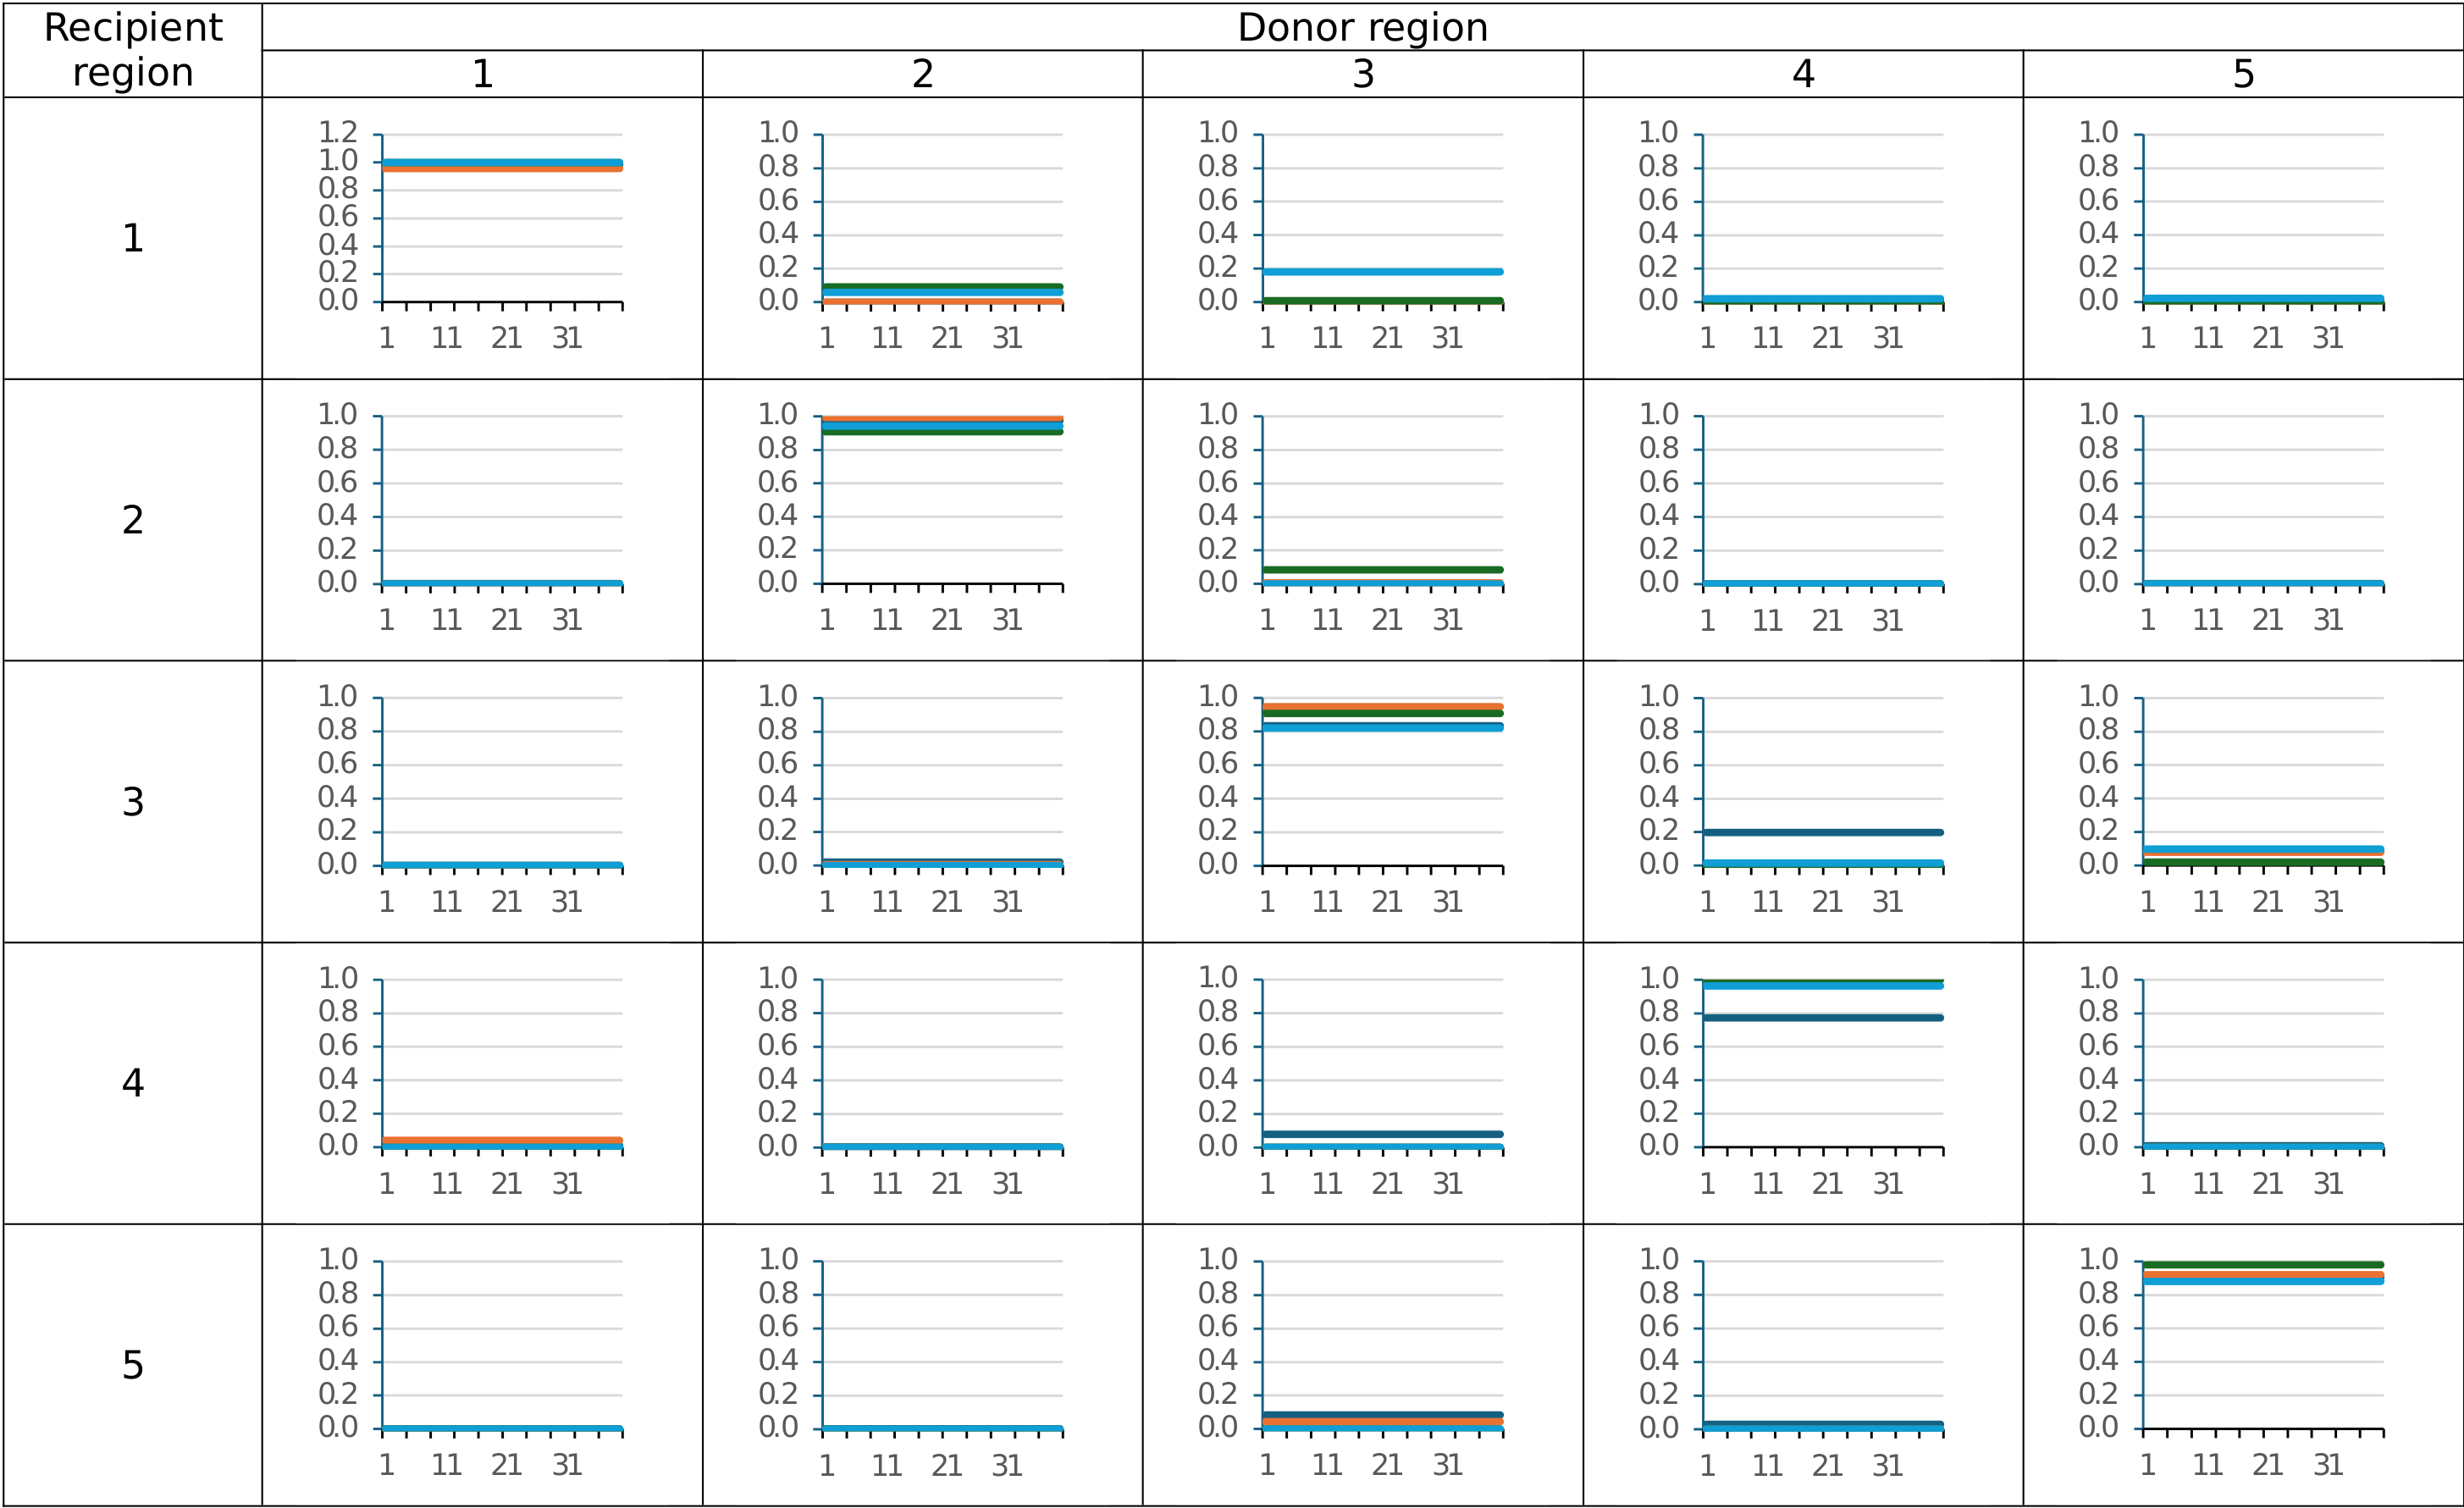
\includegraphics[width=1\linewidth,height=\textheight,keepaspectratio]{figures_new/appendix-mfcl-movement.png}

}

\caption{\label{fig-appendix-mfcl-movement}Bigeye tuna movement
probabilities estimated in the MFCL diagnostic model. Columns identify
donor regions and rows identify recipient regions; the horizontal axes
are quarterly age classes. Q1 is dark blue, Q2 orange, Q3 green and Q4
light blue.}

\end{figure}%DIF >

\end{landscape}

\clearpage

\begin{landscape}

\begin{figure}[H]

\centering{

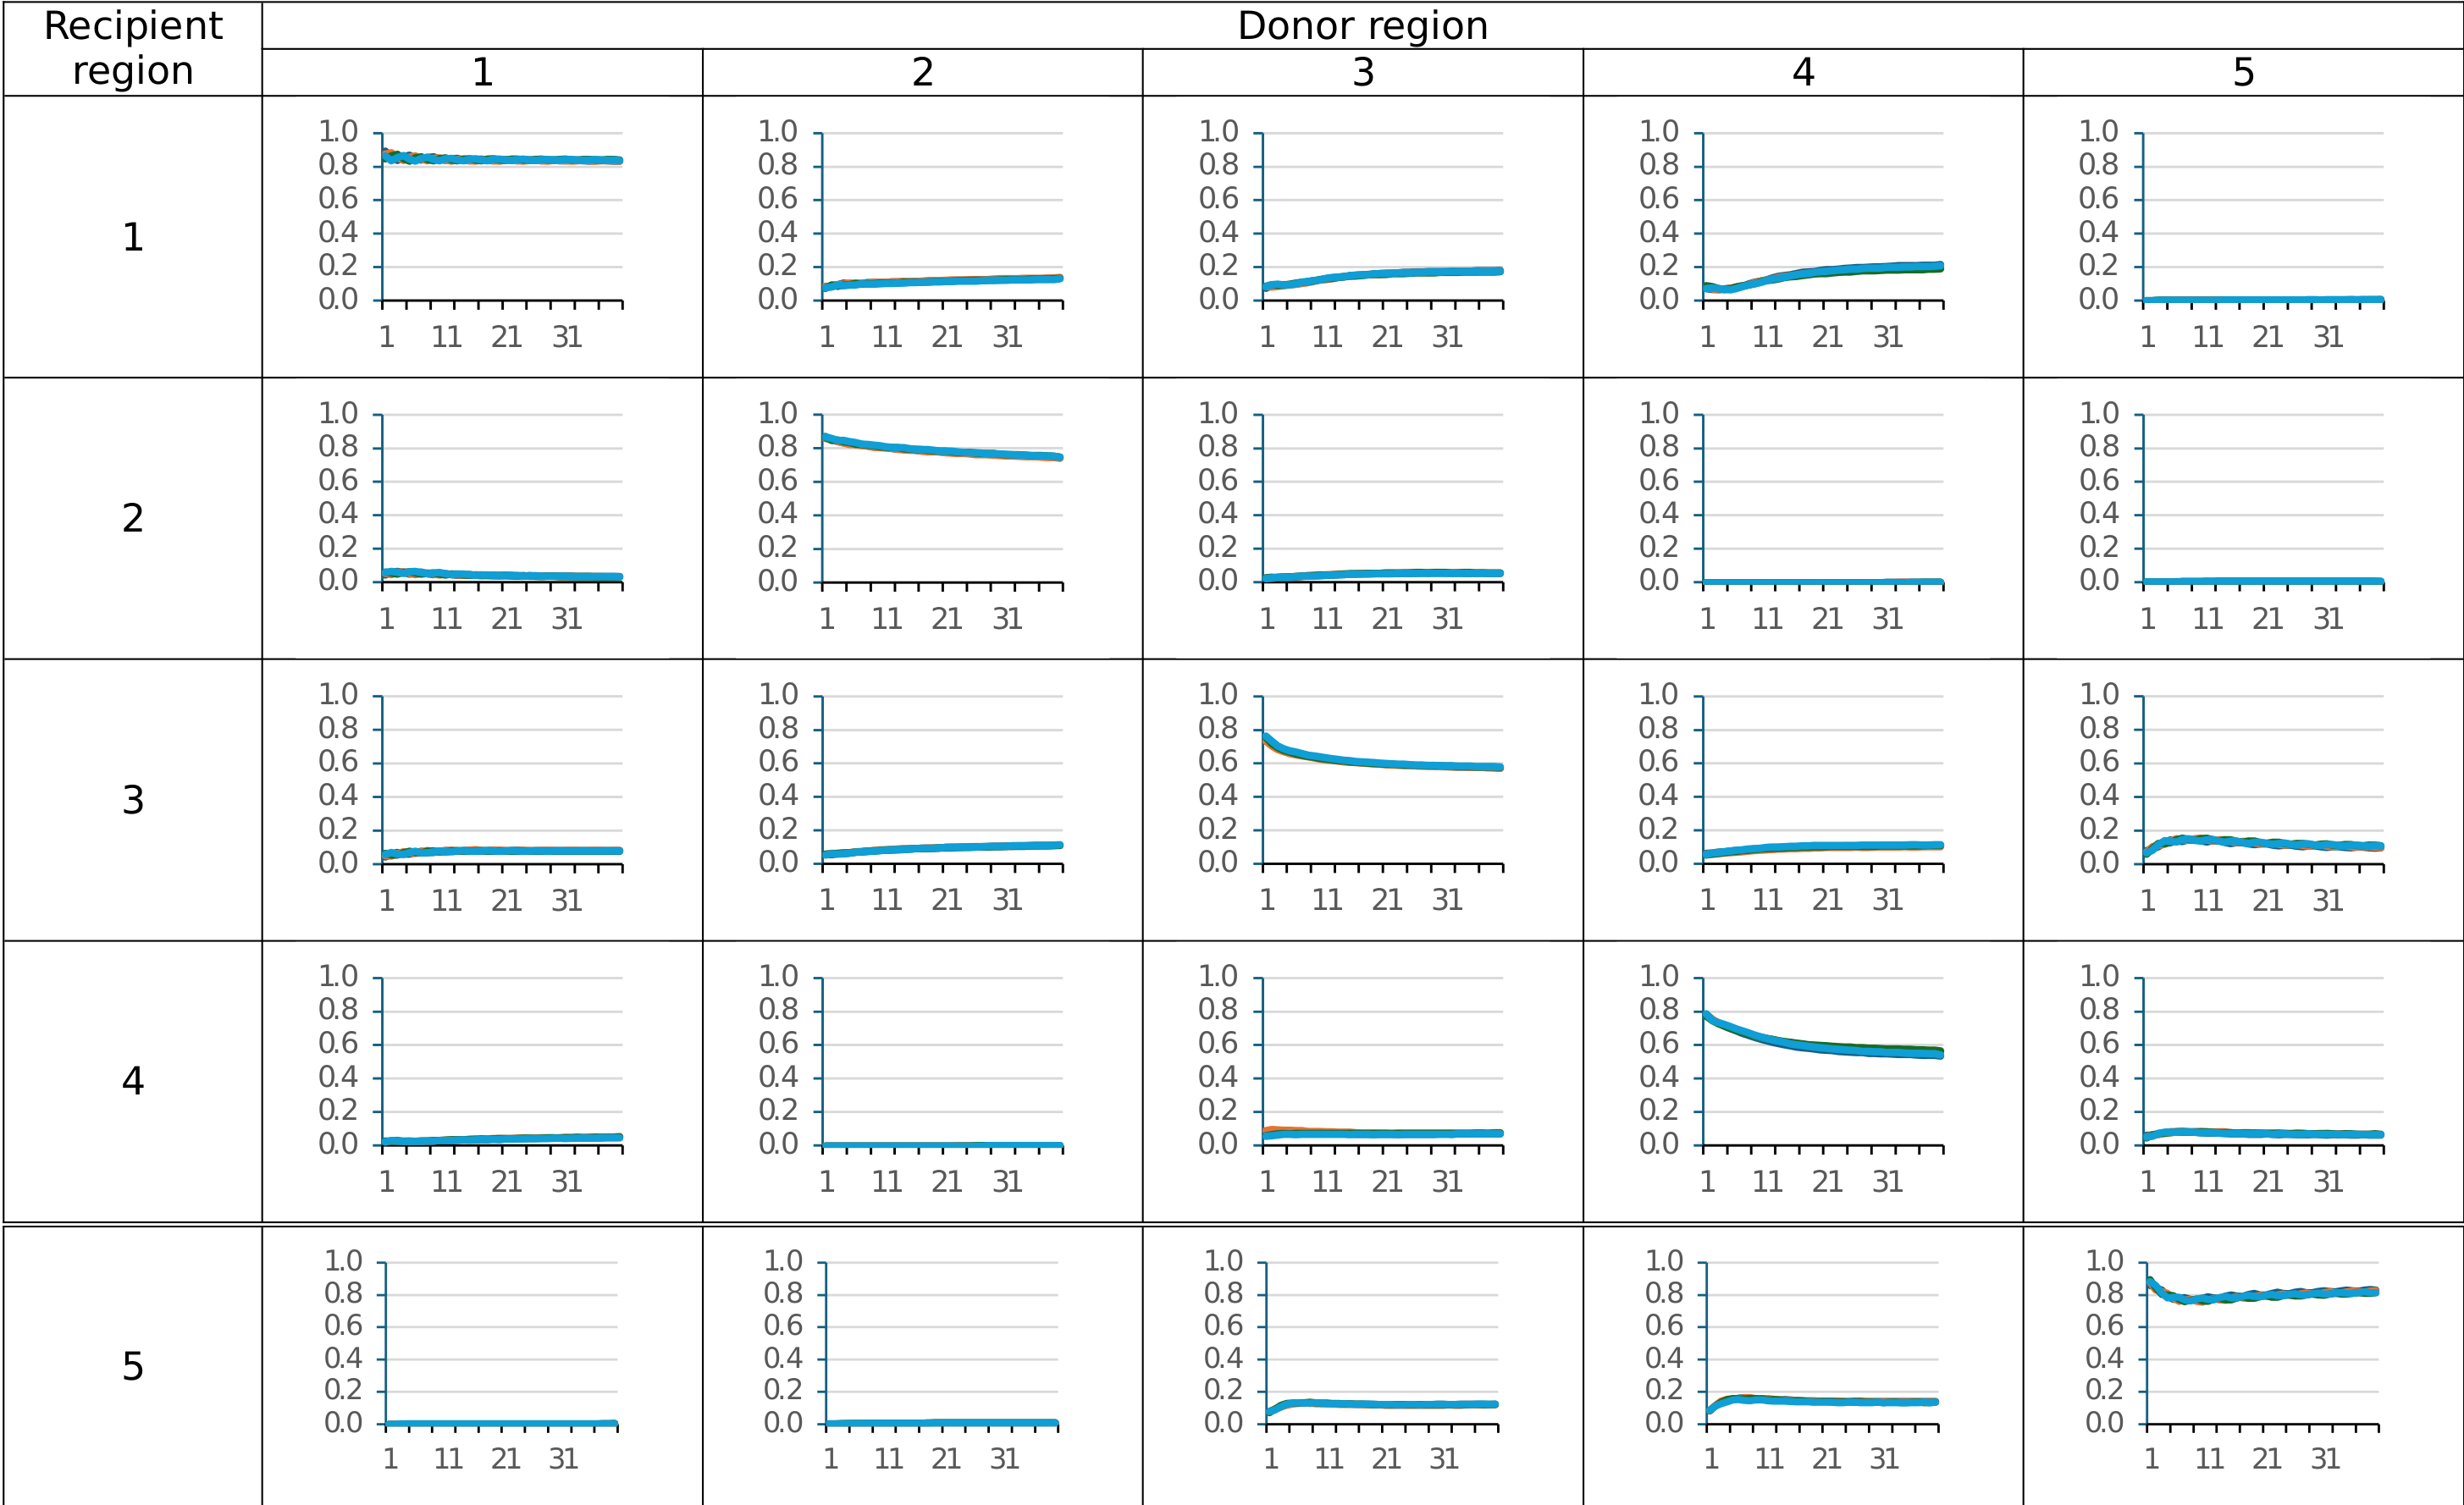
\includegraphics[width=1\linewidth,height=\textheight,keepaspectratio]{figures_new/appendix-seapodym-movement.png}

}

\caption{\label{fig-appendix-seapodym-movement}Bigeye tuna movement
probabilities from the SEAPODYM reference model. Columns identify donor
regions and rows identify recipient regions; the horizontal axes are
quarterly age classes. Q1 is dark blue, Q2 orange, Q3 green and Q4 light
blue.}

\end{figure}%DIF >

\end{landscape}

\clearpage

\DIFadd{Estimates of recruitment, spawning biomass, spawning-biomass depletion
and regional spawning-biomass distribution are shown for the diagnostic
model (5R-Diag) and the three alternatives in
Figure~\ref{fig-appendix-no-tag-comparison}. Regional-distribution
estimates are not available from the single-region model, so the
corresponding panel includes the native SEAPODYM distribution for
comparison.
}

\DIFadd{Overall, the headline estimates were reasonably consistent across
models:
}

\begin{itemize}
\item
  \textbf{\DIFadd{Recruitment (1952--2024):}} \DIFadd{the 5R-Diag average was 17.3
  million fish per quarter. The 5R-MFCL average was 14\% higher, 5R-SEAP
  was almost identical and 1R was 8\% lower.
}\item
  \textbf{\DIFadd{Spawning biomass (1952--2024):}} \DIFadd{the 5R-Diag average was 597
  thousand t. The 5R-MFCL average was 9\% higher, 5R-SEAP was 22\% lower
  and 1R was 24\% higher.
}\item
  \textbf{\DIFadd{Spawning-biomass depletion (2020--2024):}} \DIFadd{the 5R-Diag average
  was 0.18. The 5R-MFCL average was 9\% higher, 5R-SEAP was 15\% lower
  and 1R was 5\% higher.
}\item
  \textbf{\DIFadd{Regional spawning-biomass distribution (1952--2024):}} \DIFadd{5R-MFCL
  was most similar to 5R-Diag. The 5R-SEAP distribution was very similar
  to native SEAPODYM and placed considerably more spawning biomass in
  region 1 than did 5R-Diag and 5R-MFCL.
}\end{itemize}

\clearpage

\begin{landscape}

\begin{figure}[H]

\centering{

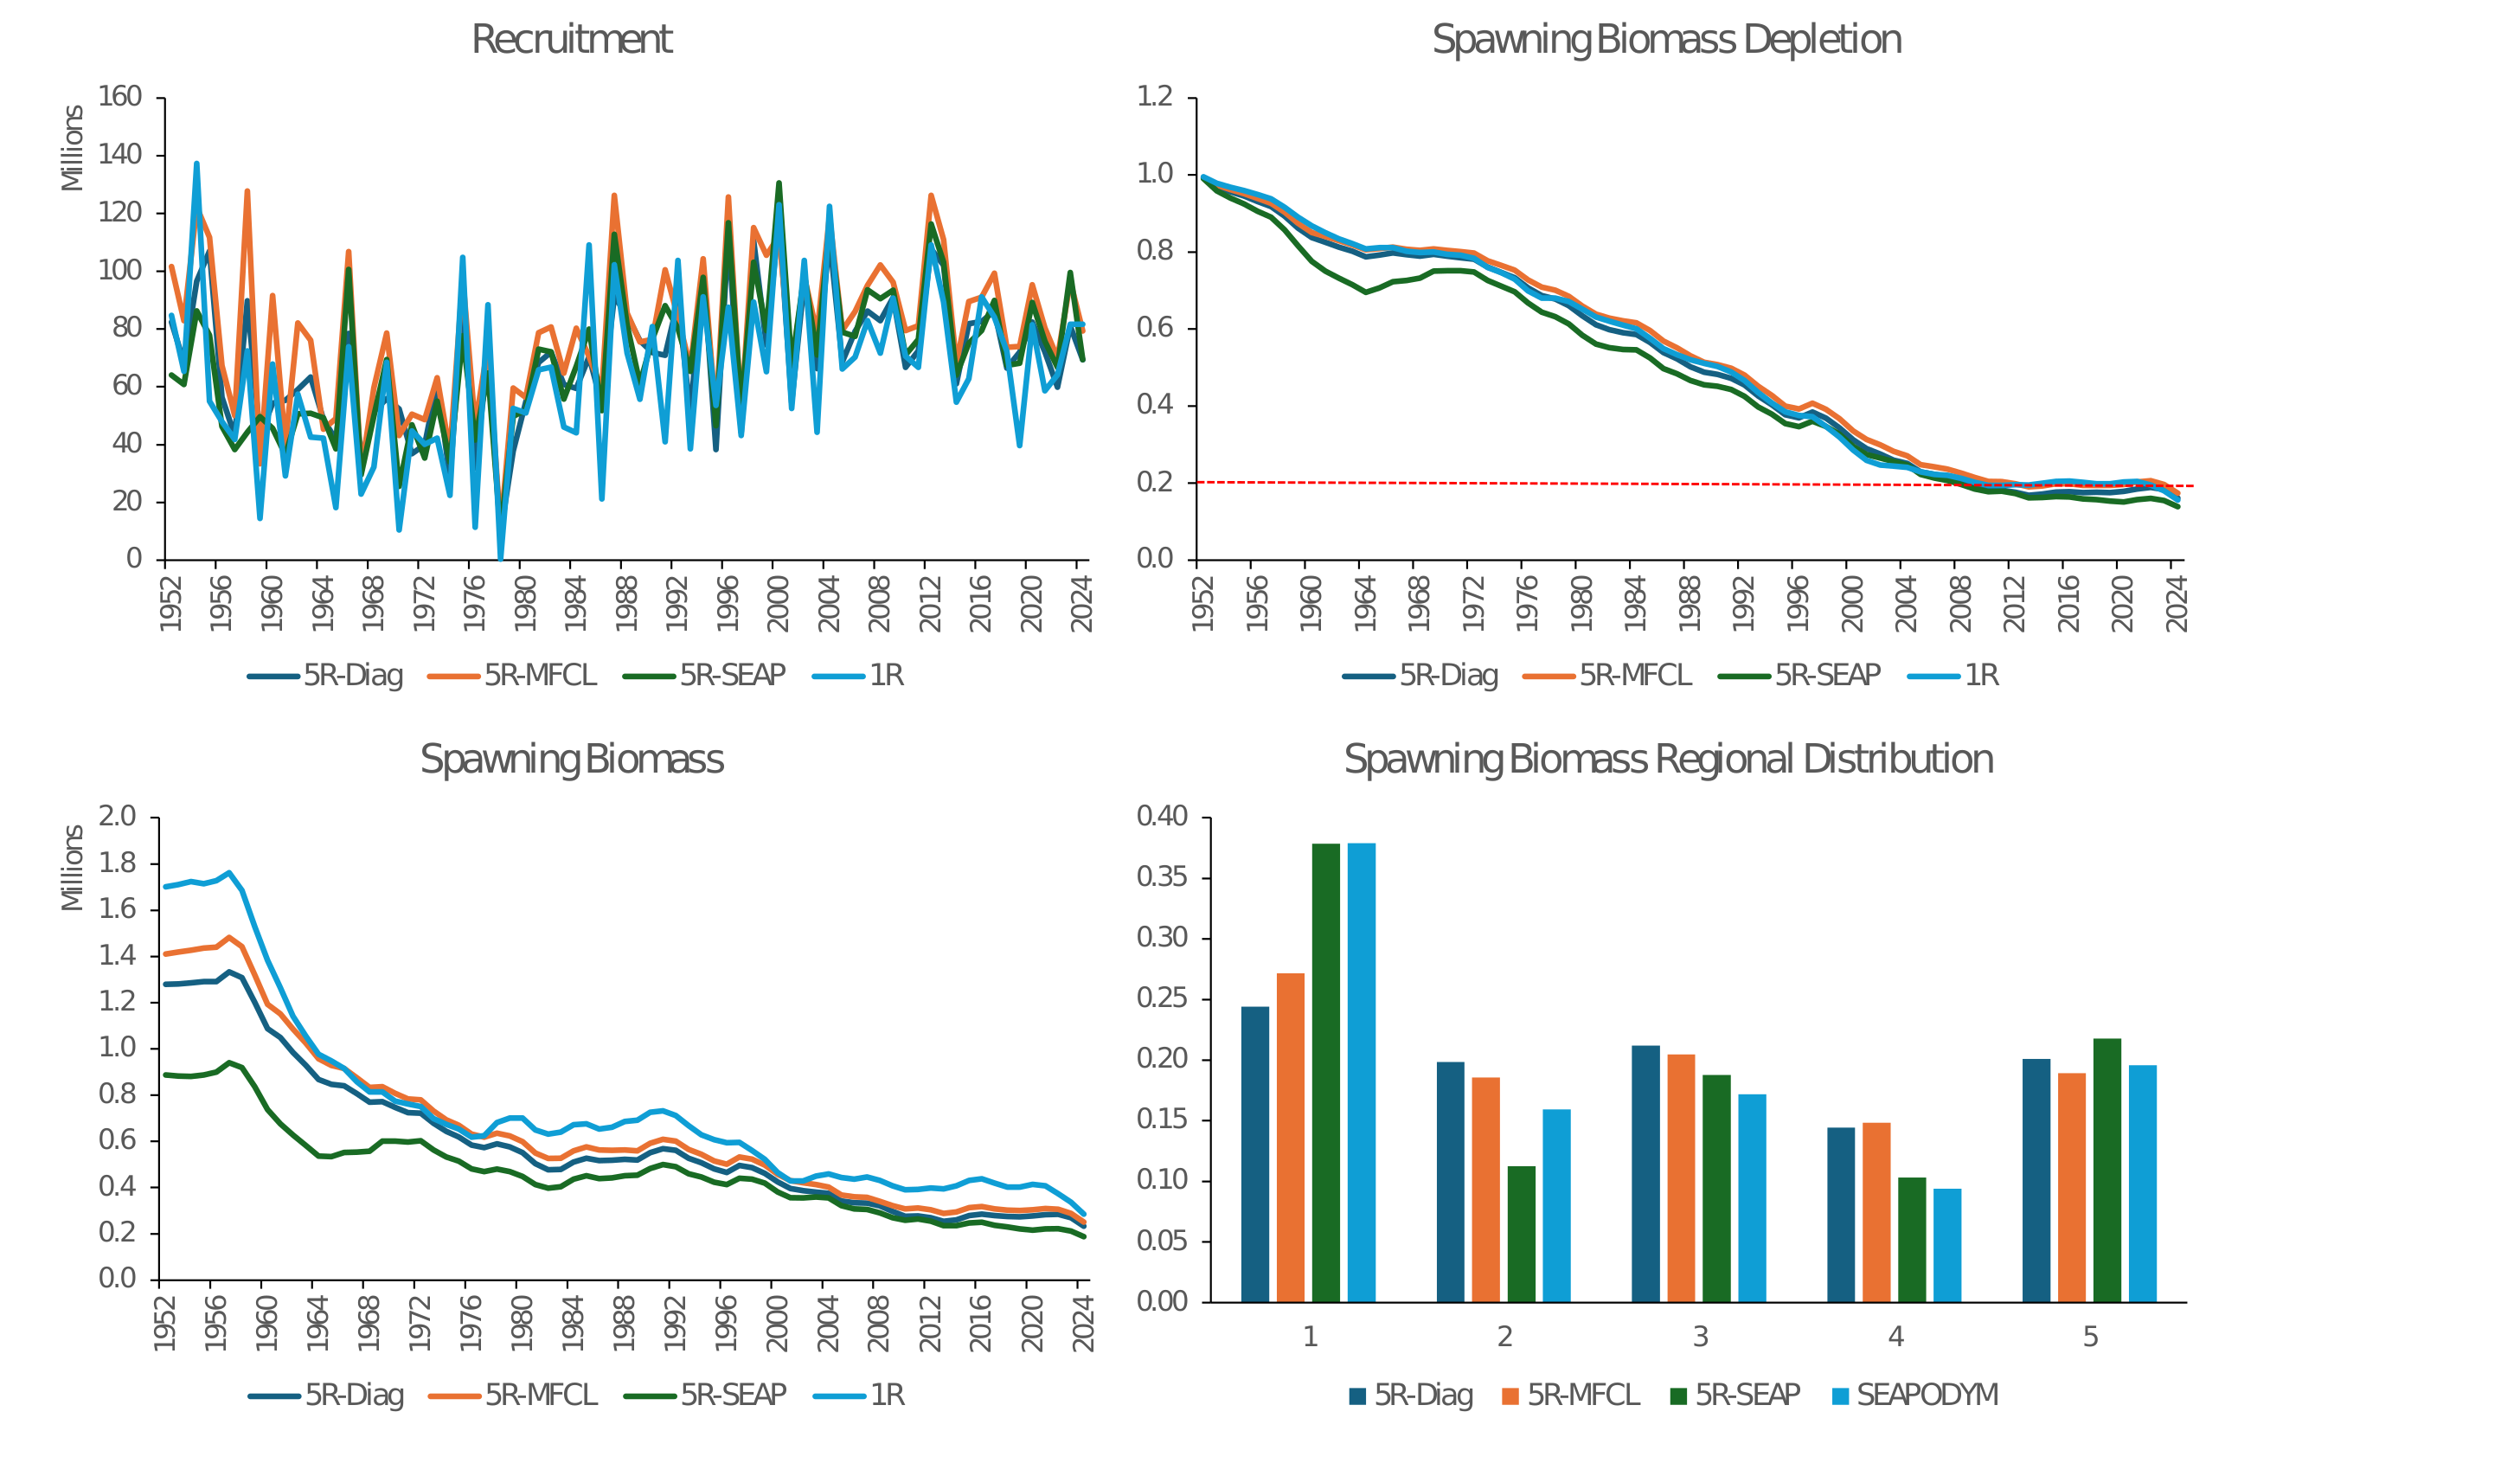
\includegraphics[width=1\linewidth,height=\textheight,keepaspectratio]{figures_new/appendix-no-tag-model-comparison.png}

}

\caption{\label{fig-appendix-no-tag-comparison}Comparisons of
recruitment (upper left), spawning-biomass depletion (upper right),
spawning biomass (lower left) and regional spawning-biomass distribution
(lower right). The models are the current five-region diagnostic model
(5R-Diag), the five-region model without tagging data and with fixed
MFCL movement (5R-MFCL), the five-region model without tagging data and
with fixed SEAPODYM movement (5R-SEAP), and the single-region model
without tagging data (1R). Native SEAPODYM is included only in the
regional-distribution panel.}

\end{figure}%DIF >

\end{landscape}

\clearpage

\subsubsection{\DIFadd{Conclusions}}\label{sec-appendix-no-tag-conclusions}

\DIFadd{The key estimates from 5R-Diag and the no-tagging model with the same
fixed movement parameters (5R-MFCL) are very similar. This indicates
either that tagging data have only a small direct effect on population
scaling in the diagnostic model, or that their effect is expressed
primarily through movement. Because the tagging-data likelihood profile
favours greater population scaling, the second explanation is credible.
A likelihood profile of the diagnostic model with movement fixed may
help distinguish these explanations.
}

\DIFadd{SEAPODYM estimates somewhat greater movement and mixing than the
diagnostic model. In MFCL, tagging observations are aggregated into
large regions, making assumptions about within-region mixing sensitive
to the spatial distributions of tag releases and fishing effort.
SEAPODYM operates at a finer \(2^\circ \times 2^\circ\) spatial
resolution and analyses tagging data in recapture-conditioned mode,
making it less dependent on reporting-rate assumptions. These features
provide a case that SEAPODYM movement may be less affected by
large-region aggregation and more realistic because environmental
drivers are represented explicitly.
}

\DIFadd{Despite the different bases for estimating movement in MFCL and
SEAPODYM, and some differences in the movement estimates themselves, the
consistency of the headline assessment quantities is reassuring.
}\DIFaddend

\section*{References}\label{references}
\addcontentsline{toc}{section}{References}

\phantomsection\label{refs}
\begin{CSLReferences}{1}{0}
\bibitem[\citeproctext]{ref-aires-da-silva_improved_2015}
Aires-da-Silva, A. M., Maunder, M. N., Schaefer, K. M., \& Fuller, D. W.
(2015). Improved growth estimates from integrated analysis of direct
aging and tag-recapture data: An illustration with bigeye tuna (thunnus
obesus) of the eastern pacific ocean with implications for management.
\emph{Fisheries Research}, \emph{163}, 119--126.

\bibitem[\citeproctext]{ref-anderson_sdmtmb_2022}
Anderson, S. C., Ward, E. J., English, P. A., \& Barnett, L. A. K.
(2022). \emph{{sdmTMB}: An r package for fast, flexible, and
user-friendly generalized linear mixed effects models with spatial and
spatiotemporal random fields} {[}Preprint{]}. Ecology.
\url{https://doi.org/10.1101/2022.03.24.485545}

\bibitem[\citeproctext]{ref-berger_analysis_2014}
Berger, A. M., McKechnie, S., Abascal, F., Kumasi, B., Usu, T., \&
Nichol, S. J. (2014). \emph{Analysis of tagging data for the 2014
tropical tuna assessments: Data quality rules, tagger effects, and
reporting rates} ({WCPFC}-{SC}10-2014/{SA}-{IP}-06). WCPFC.

\bibitem[\citeproctext]{ref-cadigan_local_2005}
Cadigan, N. G., \& Farrell, P. J. (2005). Local influence diagnostics
for the retrospective problem in sequential population analysis.
\emph{{ICES} Journal of Marine Science: Journal Du Conseil},
\emph{62}(2), 256--265.
\url{https://doi.org/10.1016/j.icesjms.2004.11.015}

\DIFaddbegin \bibitem[\citeproctext]{ref-carvalho_cookbook_2021}
\DIFadd{Carvalho, F., Winker, H., Courtney, D., Kapur, M., Kell, L., Cardinale,
M., Schirripa, M., Kitakado, T., Yemane, D., Piner, K. R., Maunder, M.
N., Taylor, I., Wetzel, C. R., Doering, K., Johnson, K. F., \& Methot,
R. D. (2021). A cookbook for using model diagnostics in integrated stock
assessments. }\emph{\DIFadd{Fisheries Research}}\DIFadd{, }\emph{\DIFadd{240}}\DIFadd{, 105959.
}\url{https://doi.org/10.1016/j.fishres.2021.105959}

\DIFaddend \bibitem[\citeproctext]{ref-castillo_jordan_stock_2022}
Castillo Jordan, C., Teears, T., Hampton, J., Davies, N., Scutt
Phillips, J., McKechnie, S., Peatman, T., Macdonald, J., Day, J.,
Magnusson, A., Scott, R., Scott, F., Pilling, G., \& Hamer, P. (2022).
\emph{Stock assessment of skipjack tuna in the western and central
pacific ocean: 2022} ({WCPFC}-{SC}18-{SA}-{WP}-01). WCPFC.

\bibitem[\citeproctext]{ref-chow_genetic_2000}
Chow, S., Okamoto, H., Miyabe, N., Hiramatsu, K., \& Barut, N. (2000).
Genetic divergence between atlantic and indo-pacific stocks of bigeye
tuna (thunnus obesus) and admixture around south africa. \emph{Molecular
Ecology}, \emph{9}(2), 221--227.
\url{https://doi.org/10.1046/j.1365-294x.2000.00851.x}

\bibitem[\citeproctext]{ref-davies_developments_2026}
Davies, N., Bouye, F., Kim, K., Magnusson, A., \& Hampton, J. (2026a).
\emph{Developments in the {MULTIFAN}-{CL} software 2025-26}
({WCPFC}-{SC}22-2026/{SA}-{IP}-02). WCPFC.

\bibitem[\citeproctext]{ref-davies_multifan-cl_2026}
Davies, N., Fournier, D. A., Hampton, J., Kleiber, P., Bouye, F., Kim,
K., Magnusson, A., \& Hoyle, S. (2026b). \emph{{MULTIFAN}-{CL} user's
guide version 2.2.7.8}. WCPFC.

\bibitem[\citeproctext]{ref-davies_developments_2019}
Davies, N., Fournier, D., \& Hampton, J. (2019). \emph{Developments in
the {MULTIFAN}-{CL} software 2018-2019}
({WCPFC}-{SC}15-2019/{SA}-{IP}-02). WCPFC.

\bibitem[\citeproctext]{ref-davies_stock_2011}
Davies, N., Hoyle, S., Harley, S., Langley, A., Kleiber, P., \& Hampton,
J. (2011). \emph{Stock assessment of bigeye tuna in the western and
central pacific ocean} ({WCPFC}-{SC}7-2011/{SA}-{WP}-02). WCPFC.

\bibitem[\citeproctext]{ref-day_stock_2023}
Day, J., Magnusson, A., Teears, T., Hampton, J., Davies, N., Castillo
Jordán, C., Peatman, T., Scott, R., Scutt Phillips, J., McKechnie, S.,
Scott, F., Yao, N., Natadra, R., Pilling, G., Williams, P., \& Hamer, P.
(2023). \emph{Stock assessment of bigeye tuna in the western and central
pacific ocean: 2023} ({WCPFC}-{SC}19-2023/{SA}-{WP}-05 (Rev. 2)). WCPFC.

\DIFaddbegin \bibitem[\citeproctext]{ref-deroba_simulation_2015}
\DIFadd{Deroba, J. J., Butterworth, D. S., Methot, R. D., De Oliveira, J. A. A.,
Fernandez, C., Nielsen, A., Cadrin, S. X., Dickey-Collas, M., Legault,
C. M., Ianelli, J., Valero, J. L., Needle, C. L., O'Malley, J. M.,
Chang, Y.-J., Thompson, G. G., Canales, C., Swain, D. P., Miller, D. C.
M., Hintzen, N. T., \ldots{} Hulson, P.-J. F. (2015). Simulation testing
the robustness of stock assessment models to error: Some results from
the }{\DIFadd{ICES}} \DIFadd{strategic initiative on stock assessment methods. }\emph{\DIFadd{ICES
Journal of Marine Science}}\DIFadd{, }\emph{72}(1)\DIFadd{, 19--30.
}\url{https://doi.org/10.1093/icesjms/fst237}

\DIFaddend \bibitem[\citeproctext]{ref-ducharme-barth_natural_2026}
Ducharme-Barth, N., Peatman, T., Scutt Phillips, J., \& Minte-Vera, C.
(2026). \emph{Natural mortality estimation for {WCPO} bigeye tuna: A
joint cohort analysis of coral sea and region 4 tagging data}
({WCPFC}-{SC}22-2026/{SA}-{IP}-14). WCPFC.

\bibitem[\citeproctext]{ref-ducharme-barth_stock_2020}
Ducharme-Barth, N., Vincent, M., Hampton, J., Hamer, P., Williams, P.,
\& Pilling, G. (2020a). \emph{Stock assessment of bigeye tuna in the
western and central pacific ocean} ({WCPFC}-{SC}16-2020/{SA}-{WP}-03
{[}{REV}3{]}). WCPFC.

\bibitem[\citeproctext]{ref-ducharme-barth_analysis_2020}
Ducharme-Barth, N., Vincent, M., Vidal, T., \& Hamer, P. (2020b).
\emph{Analysis of pacific-wide operational longline dataset for bigeye
and yellowfin tuna catch-per-unit-effort ({CPUE})}
({SC}16-{SA}-{IP}-07). WCPFC.

\bibitem[\citeproctext]{ref-evans_behaviour_2008}
Evans, K., Langley, A., Clear, N. P., Williams, P., Patterson, T.,
Sibert, J., Hampton, J., \& Gunn, J. S. (2008). Behaviour and habitat
preferences of bigeye tuna (thunnus obesus) and their influence on
longline fishery catches in the western coral sea. \emph{Canadian
Journal of Fisheries and Aquatic Sciences}, \emph{65}, 2427--2443.

\bibitem[\citeproctext]{ref-eveson_integrated_2020}
Eveson, P., Vincent, M., Farley, J., Krusic-Golub, K., \& Hampton, J.
(2020). \emph{Integrated growth models from otolith and tagging data for
yellowfin and bigeye tuna in the western and central pacific ocean}
({SC}16-{SA}-{IP}-03). WCPFC.

\bibitem[\citeproctext]{ref-farley_age_2017}
Farley, J., Eveson, P., Krusic-Golub, K., Sanchez, C., Rouspard, F.,
McKechnie, S., Nichol, S., Leroy, B., Smith, N., \& Chang, S.-K. (2017).
\emph{Age, growth and maturity of bigeye tuna in the pacific}
({WCPFC}-{SC}13- 2017/{SA}-{WP}-01). WCPFC.

\bibitem[\citeproctext]{ref-farley_age_2020}
Farley, J., Krusic-Golub, K., Eveson, P., Clear, N., Rouspard, F.,
Sanchez, C., Nicol, S., \& Hampton, J. (2020). \emph{Age and growth of
yellowfin and bigeye tuna in the western and central pacific ocean from
otoliths} ({SC}16-{SA}-{WP}-02). WCPFC.

\bibitem[\citeproctext]{ref-fournier_multifan-cl_1998}
Fournier, D. A., Hampton, J., \& Sibert, J. R. (1998). {MULTIFAN}-{CL}:
A length-based, age-structured model for fisheries stock assessment,
with application to south pacific albacore, thunnus alalunga.
\emph{Canadian Journal of Fisheries and Aquatic Sciences}, \emph{55},
2105--2116.

\bibitem[\citeproctext]{ref-fournier_ad_2012}
Fournier, D. A., Skaug, H. J., Ancheta, J., Ianelli, J., Magnusson, A.,
Maunder, M. N., Nielson, A., \& Sibert, J. (2012). {AD} model builder:
Using automatic differentiation for statistical inference of highly
parameterized complex nonlinear models. \emph{Optimization Methods and
Software}, \emph{27}(2), 233--249.

\bibitem[\citeproctext]{ref-fournier_general-theory_1982}
Fournier, D., \& Archibald, C. P. (1982). A general-theory for analyzing
catch at age data. \emph{Canadian Journal of Fisheries and Aquatic
Sciences}, \emph{39}(8), 1195--1207.
\url{https://doi.org/10.1139/f82-157}

\bibitem[\citeproctext]{ref-francis_use_1992}
Francis, R. I. C. C. (1992). Use of risk analysis to assess fishery
management strategies: A case study using orange roughy
({\emph{Hoplostethus atlanticus}}) on the chatham rise, new zealand.
\emph{Canadian Journal of Fisheries and Aquatic Science}, \emph{49},
922--930.

\bibitem[\citeproctext]{ref-francis_data_2011}
Francis, R. I. C. C. (2011). Data weighting in statistical fisheries
stock assessment models. \emph{Canadian Journal of Fisheries and Aquatic
Sciences}, \emph{68}, 1124--1138.

\bibitem[\citeproctext]{ref-gonzalez_genetic_2008}
Gonzalez, E. G., Beerli, P., \& Zardoya, R. (2008). Genetic structuring
and migration patterns of atlantic bigeye tuna, thunnus obesus (lowe,
1839). \emph{{BMC} Evolutionary Biology}, \emph{8}(1), 252.
\url{https://doi.org/10.1186/1471-2148-8-252}

\bibitem[\citeproctext]{ref-grewe_assessment_1998}
Grewe, P. M., \& Hampton, J. (1998). \emph{An assessment of bigeye
(thunnus obesus) population structure in the pacific ocean based on
mitochondrial {DNA} and {DNA} microsatellite analysis}. {JIMAR}
Contribution 98-330.

\bibitem[\citeproctext]{ref-grewe_population_2019}
Grewe, P. M., Wudianto, C. H., Proctor, C. H., Adam, M. S., Jauhary, A.
R., Schaefer, K., Itano, D. G., Evans, K., Killian, A., Foster, S. D.,
Gosselin, T., Feutry, P., Aulich, J., Gunasekera, R. M., Lansdell, M.,
\& Davies, C. R. (2019). \emph{Population structure and connectivity of
tropical tuna species across the indo pacific ocean region}
({WCPFC}-{SC}15-2019/{SA}-{IP}-15). WCPFC.

\DIFdelbegin \bibitem[\citeproctext]{ref-hamel_method_2015}
\DIFdel{Hamel, O. S. (2015). A method for calculating a meta-analytical prior
for the natural mortality rate using multiple life history correlates.
}\emph{\DIFdel{Ices Journal of Marine Science}}%DIFAUXCMD
\DIFdel{, }%DIFDELCMD < \emph{72}(1)%%%
\DIFdel{, 62--69.
}%DIFDELCMD < \url{https://doi.org/10.1093/icesjms/fsu131}
%DIFDELCMD <

%DIFDELCMD < %%%
\DIFdelend \bibitem[\citeproctext]{ref-hamer_summary_2026}
Hamer, P. (2026). \emph{Summary report from the {SPC} pre-assessment
workshop - march 2026} ({WCPFC}-{SC}22-2026/{SA}-{IP}-01). WCPFC.

\bibitem[\citeproctext]{ref-hamer_wcpfc_2026}
Hamer, P., Castillo Jordán, C., Panizza, A., \& Peatman, T. (2026).
\emph{{WCPFC} Project127/127a - review and reconciliation of size data
collected in the {WCPFC}-{CA} for stock assessment purposes: Phase 2
progress report} ({WCPFC}-{SC}22-2026/{ST}-{WP}-02). WCPFC.

\bibitem[\citeproctext]{ref-hamer_review_2023}
Hamer, P., Potts, J., Macdonald, J., \& Senina, I. (2023). \emph{Review
and analyses to inform conceptual models of population structure and
spatial stratification of bigeye and yellowfin tuna assessments in the
western and central pacific ocean} ({SC}19-{SA}-{WP}-02). WCPFC.

\bibitem[\citeproctext]{ref-hamer_progress_2025}
Hamer, P., Schneiter, E., Vidal, T., \& Williams, P. (2025).
\emph{Progress report: Review and reconciliation of size data collected
in the {WCPFC}-{CA} for stock assessment purposes ({WCPFC} project:
127)} ({WCPFC}-{SC}21-{ST}-{WP}-02). WCPFC.

\bibitem[\citeproctext]{ref-hampton_natural_2000}
Hampton, J. (2000). Natural mortality rates in tropical tunas: Size
really does matter. \emph{Canadian Journal of Fisheries and Aquatic
Science}, \emph{57}, 1002--1010.

\bibitem[\citeproctext]{ref-hampton_investigation_2026-1}
Hampton, J., Davies, N., \& Hamer, P. (2026a). \emph{Investigation of
the impacts of regional growth variation on the 2023 bigeye tuna stock
assessment} ({WCPFC}-{SC}22-2026/{SA}-{IP}11). WCPFC.

\bibitem[\citeproctext]{ref-hampton_spatially-disaggregated_2001}
Hampton, J., \& Fournier, D. A. (2001). A spatially-disaggregated,
length-based, age-structured population model of yellowfin tuna (thunnus
albacares) in the western and central pacific ocean. \emph{Marine and
Freshwater Research}, \emph{52}, 937--963.

\bibitem[\citeproctext]{ref-hampton_investigation_2026}
Hampton, J., Teears, T., Kim, K., Magnusson, A., Davies, N., \& Hamer,
P. (2026b). \emph{Investigation of single region fleets as areas models
for bigeye and yellowfin tuna in the {WCPO}}
({WCPFC}-{SC}22-2026/{SA}-{IP}-09). WCPFC.

\bibitem[\citeproctext]{ref-hampton_annual_2016}
Hampton, J., \& Williams, P. (2016). \emph{Annual estimates of purse
seine catches by species based on alternative data sources}
({WCPFC}-{SC}12-2016/{ST}-{IP}-03). WCPFC.

\bibitem[\citeproctext]{ref-hare_western_2025}
Hare, S., Vidal, T., Castillo Jordán, C., Day, J., Hamer, P., Hill, N.,
Machful, P., Magnusson, A., Nicol, S., Odongo, V., Panizza, A., Peatman,
T., Scott, R., Senina, I., Sloyan, B., Teears, T., \& Pilling, G.
(2025). \emph{The western and central pacific tuna fishery: 2024
overview and status of stocks} {[}Tuna Fisheries Assessment Report No.
25{]}. SPC.

\bibitem[\citeproctext]{ref-hare_compendium_2026}
Hare, S., Vidal, T., Scott, R., \& Pilling, G. (2026). \emph{A
compendium of fisheries indicators for target tuna stocks in the {WCPFC}
convention area} ({WCPFC}-{SC}22-2026/{SA}-{WP}-07). WCPFC.

\bibitem[\citeproctext]{ref-harley_preliminary_2011}
Harley, S. J. (2011). \emph{A preliminary investigation of steepness in
tunas based on stock assessment results}
({WCPFC}-{SC}7-2011/{SA}-{IP}-08). WCPFC.

\bibitem[\citeproctext]{ref-harley_stock_2014}
Harley, S. J., Davies, N., Hampton, J., \& McKechnie, S. (2014).
\emph{Stock assessment of bigeye tuna in the western and central pacific
ocean} ({WCPFC}-{SC}10-2014/{SA}-{WP}-01). WCPFC.
\url{http://wcpfc.int/system/files/SC10-SA-WP-01\%20BET\%20Assessment.pdf}

\bibitem[\citeproctext]{ref-harley_stock_2010}
Harley, S. J., Hoyle, S., Hampton, J., \& Kleiber, P. (2010).
\emph{Stock assessment of bigeye tuna in the western and central pacific
ocean} ({WCPFC}-{SC}6-2010/{SA}-{WP}-01). WCPFC.

\bibitem[\citeproctext]{ref-harley_simple_2003}
Harley, S. J., \& Maunder, M. N. (2003). \emph{A simple model for
age-structured natural mortality based on changes in sex ratios}
({SAR}-4-01). Inter-American Tropical Tuna Commission.

\bibitem[\citeproctext]{ref-harley_stock_2009}
Harley, S., Hoyle, S., \& Langley, A. (2009). \emph{Stock assessment of
bigeye tuna in the western and central pacific ocean.}
({WCPFC}-{SC}5-2009/{SA}-{WP}-04). WCPFC.

\bibitem[\citeproctext]{ref-hasegawa_new_2026}
Hasegawa, T., Okamoto, K., Ijima, H., Kim, K., Hamer, P., Wakefield, C.,
Pons, A., Widdrington, J., \& Davies, N. (2026). \emph{New age-at-length
data for {WCPO} bigeye and yellowfin tuna from the temperate north
pacific and approaches to address spatial sampling bias in growth
estimation within {MFCL}} ({WCPFC}-{SC}22-2026/{IP}-08). WCPFC.

\bibitem[\citeproctext]{ref-hoyle_effort_2024}
Hoyle, S. (2024). \emph{Effort creep in longline and purse seine {CPUE}
and its application in tropical tuna assessments}
({WCPFC}-{SC}20-2024/{SA}-{IP}-09). WCPFC.

\bibitem[\citeproctext]{ref-hoyle_adjusted_2008}
Hoyle, S. D. (2008). \emph{Adjusted biological parameters and spawning
biomass calculations for south pacific albacore tuna, and their
implications for stock assessments} ({WCPFC}-{SC}4-2008/{ME}-{WP}-02).
WCPFC.

\bibitem[\citeproctext]{ref-hoyle_sensitivity_2008}
Hoyle, S., \& Nicol, S. (2008). \emph{Sensitivity of bigeye stock
assessment to alternative biological and reproductive assumptions}
({WCPFC}-{SC}4-2008/{ME}-{WP}-01). WCPFC.

\bibitem[\citeproctext]{ref-hurtado-ferro_looking_2015}
Hurtado-Ferro, F., Szuwalski, C. S., Valero, J. L., Anderson, S. C.,
Cunningham, C. J., Johnson, K. F., Licandeo, R., McGilliard, C. R.,
Monnahan, C. C., Muradian, M. L., Ono, K., Vert-Pre, K. A., Whitten, A.
R., \& Punt, A. E. (2015). Looking in the rear-view mirror: Bias and
retrospective patterns in integrated, age-structured stock assessment
models. \emph{Ices Journal of Marine Science}, \emph{72}(1), 99--110.
\url{https://doi.org/10.1093/icesjms/fsu198}

\bibitem[\citeproctext]{ref-ianelli_independent_2012}
Ianelli, J., Maunder, M. N., \& Punt, Andre. E. (2012).
\emph{Independent review of the 2011 {WCPO} bigeye tuna assessment}
({WCPFC}-{SC}8-2012/{SA}-{WP}-01). WCPFC.

\bibitem[\citeproctext]{ref-ijima_tuna_2023}
Ijima, H., \& Jusup, M. (2023). \emph{Tuna and billfish larval
distributions in a warming ocean}. {arXiv}.
\url{http://arxiv.org/abs/2304.09442}

\bibitem[\citeproctext]{ref-issf_report_2011}
ISSF. (2011). \emph{Report of the 2011 {ISSF} stock assessment workshop}
({ISSF} Technical Report 2011-02). ISSF.

\bibitem[\citeproctext]{ref-itano_reproductive_2000}
Itano, D. (2000). \emph{The reproductive biology of yellowfin tuna
({\emph{Thunnus albacares}}) in hawaiian waters and the western tropical
pacific ocean: Project summary} (JIMAR Contribution 00-328 {SOEST}
00-01). University of Hawai'i.

\DIFaddbegin \bibitem[\citeproctext]{ref-kim_quantitative_2025}
\DIFadd{Kim, K., \& Neubauer, P. (2025). A quantitative evaluation of the
pollock }{\DIFadd{Gadus chalcogrammus}} \DIFadd{restocking programme in south korea.
}\emph{\DIFadd{Canadian Journal of Fisheries and Aquatic Sciences}}\DIFadd{, }\emph{\DIFadd{82}}\DIFadd{,
1--20. }\url{https://doi.org/10.1139/cjfas-2024-0375}

\bibitem[\citeproctext]{ref-kim_enhancing_2024}
\DIFadd{Kim, K., Sibanda, N., Arnold, R., \& A'mar, T. (2024). Enhancing
data-limited assessments with random effects: A case study on korea chub
mackerel (}{\DIFadd{Scomber japonicus}}\DIFadd{). }\emph{\DIFadd{Canadian Journal of Fisheries and
Aquatic Sciences}}\DIFadd{, }\emph{81}(10)\DIFadd{, 1433--1455.
}\url{https://doi.org/10.1139/cjfas-2023-0358}

\DIFaddend \bibitem[\citeproctext]{ref-kolody_evaluation_2014}
Kolody, D., \& Hoyle, S. (2014). Evaluation of tag mixing assumptions in
western pacific ocean skipjack tuna stock assessment models.
\emph{Fisheries Research},
\emph{http://dx.doi.org/101016/j.fishres.2014.05.008}.

\bibitem[\citeproctext]{ref-langley_stock_2008}
Langley, A., Hampton, J., Kleiber, P., \& Hoyle, S. (2008). \emph{Stock
assessment of bigeye tuna in the western and central pacific ocean,
including an analysis of management options}
({WCPFC}-{SC}4/{SA}-{WP}-1). WCPFC.

\bibitem[\citeproctext]{ref-mckechnie_sensitivity_2015}
McKechnie, S., Hampton, J., Abascal, F., Davies, N., \& Harley, S. J.
(2015a). \emph{Sensitivity of {WCPO} stock assessment results to the
inclusion of {EPO} dynamics within a pacific-wide analysis}
({WCPFC}-{SC}11-2015/{SA}-{WP}-04). WCPFC.

\bibitem[\citeproctext]{ref-mckechnie_construction_2016}
McKechnie, S., Ochi, D., Kiyofuji, H., Peatman, T., \& Caillot, S.
(2016). \emph{Construction of tagging data input files for the 2016
skipjack tuna stock assessment in the western and central pacific ocean}
({WCPFC}-{SC}12-2016/{SA}-{IP}-05). WCPFC.

\bibitem[\citeproctext]{ref-mckechnie_stock_2017}
McKechnie, S., Pilling, G., \& Hampton, J. (2017a). \emph{Stock
assessment of bigeye tuna in the western and central pacific ocean}
({WCPFC}-{SC}13-2017/{SA}-{WP}-05). WCPFC.

\bibitem[\citeproctext]{ref-mckechnie_summaries_2026}
McKechnie, S., Pilling, G., \& Vidal, T. (2026). \emph{Summaries of
bigeye tuna catch and effort to support management procedure
discussions} ({WCPFC}-{SC}22-2026/{SA}-{IP}-12). WCPFC.

\bibitem[\citeproctext]{ref-mckechnie_analysis_2015}
McKechnie, S., Tremblay-Boyer, L., \& Harley, S. J. (2015b).
\emph{Analysis of pacific-wide operational longline {CPUE} data for
bigeye tuna} ({WCPFC}-{SC}11-2015/{SA}-{WP}-03). WCPFC.

\bibitem[\citeproctext]{ref-mckechnie_background_2017}
McKechnie, S., Tremblay-Boyer, L., \& Pilling, G. (2017b).
\emph{Background analyses for the 2017 stock assessments of bigeye and
yellowfin tuna in the western and central pacific ocean}
({WCPFC}-{SC}13-2017/{SA}-{IP}-06). WCPFC.

\bibitem[\citeproctext]{ref-mohn_retrospective_1999}
Mohn, R. (1999). The retrospective problem in sequential population
analysis: An investigation using cod fishery and simulated data.
\emph{Ices Journal of Marine Science}, \emph{56}(4), 473--488.
\url{https://doi.org/10.1006/jmsc.1999.0481}

\bibitem[\citeproctext]{ref-moore_defining_2020}
Moore, B. R., Bell, J. D., Evans, K., Farley, J., Grewe, P. M., Hampton,
J., Marie, A. D., Minte-Vera, C., Nicol, S., Pilling, G. M., Scutt
Phillips, J., Tremblay-Boyer, L., Williams, A. J., \& Smith, N. (2020).
Defining the stock structures of key commercial tunas in the pacific
ocean i: Current knowledge and main uncertainties. \emph{Fisheries
Research}, \emph{230}, 105525.
\url{https://doi.org/10.1016/j.fishres.2020.105525}

\bibitem[\citeproctext]{ref-moore_movement_2019}
Moore, B. R., Lestari, P., Cutmore, S. C., Proctor, C., \& Lester, R. J.
G. (2019). Movement of juvenile tuna deduced from parasite data.
\emph{{ICES} Journal of Marine Science}, \emph{76}(6), 1678--1689.
\url{https://doi.org/10.1093/icesjms/fsz022}

\bibitem[\citeproctext]{ref-natasha_no_2022}
Natasha, J., Stockwell, B. L., Marie, A. D., Hampton, J., Smith, N.,
Nicol, S., \& Rico, C. (2022). No population structure of bigeye tunas
(thunnus obesus) in the western and central pacific ocean indicated by
single nucleotide polymorphisms. \emph{Front. Mar. Sci.}, \emph{9},
799684. \url{https://doi.org/10.3389/fmars.2022.799684}

\bibitem[\citeproctext]{ref-nicol_bigeye_2011}
Nicol, S., Hoyle, S., Farley, J., Muller, B., Retalmai, S., Sisior, K.,
\& Williams, A. (2011). \emph{Bigeye tuna age, growth, and reproductive
biology (project 35)} ({WCPFC}-{SC}7-2011/{SA}-{WP}-01). WCPFC.

\bibitem[\citeproctext]{ref-nishikawa_average_1985}
Nishikawa, Y., Honma, M., Ueyanagi, S., \& Kikawa, S. (1985). Average
distribution of larvae of oceanic species of scombroid fishes,
1956-1981. \emph{Far Seas Fish.Res.Lab., 99 p.}

\bibitem[\citeproctext]{ref-peatman_better_2019}
Peatman, T., Fukofuka, S., Park, T., Williams, P., Hampton, J., \&
Smith, N. (2019). \emph{Better purse seine catch composition estimates:
Progress on the project 60 work plan.} {[}Technical Report{]}. SPC.

\bibitem[\citeproctext]{ref-peatman_analysis_2026-2}
Peatman, T., Gislard, S., Scutt Phillips, J., Potts, J., \& Nicol, S.
(2026a). \emph{Analysis of tag seeding data for the 2026 yellowfin \&
bigeye assessments: Reporting rates for purse seine fleets}
({WCPFC}-{SC}22-2026/{SA}-{IP}-05). WCPFC.

\bibitem[\citeproctext]{ref-peatman_analysis_2026}
Peatman, T., Kim, K., Magnusson, A., Castillo Jordan, C., \& Hamer, P.
(2026b). \emph{Analysis of size frequency data for the 2026 bigeye and
yellowfin assessments} ({WCPFC}-{SC}22-{SA}-{IP}06). WCPFC.

\bibitem[\citeproctext]{ref-peatman_analysis_2026-1}
Peatman, T., Scutt Phillips, J., Potts, J., \& Nicol, S. (2026c).
\emph{Analysis of tagging data for the 2026 yellowfin \& bigeye
assessments: Corrections to tag releases for tagging conditions}
({WCPFC}-{SC}22-2026/{SA}-{IP}-04). WCPFC.

\bibitem[\citeproctext]{ref-peatman_project_2021}
Peatman, T., Williams, P., \& Nicol, S. (2021). \emph{Project 60:
Progress towards achieving {SC}16 recommendations}
({WCPFC}-{SC}17-2021/{ST}-{IP}-04). WCPFC.

\bibitem[\citeproctext]{ref-peatman_project_2023}
Peatman, T., Williams, P., \& Nicol, S. (2023). \emph{Project 60:
{Progress} report - improving purse seine species composition} (WCPFC
Scientific Committee Paper SC19-ST-IP-03).

\bibitem[\citeproctext]{ref-pilling_approaches_2016}
Pilling, G., Scott, R., Davies, N., \& Hampton, J. (2016).
\emph{Approaches used to undertake management projections of {WCPO} tuna
stocks based upon {MULTIFAN}-{CL} stock assessments}
({WCPFC}-{SC}12-2016/{MI}-{IP}-04). Bali, Indonesia, 3-11 August 2016.

\bibitem[\citeproctext]{ref-piner_meta-analysis_2011}
Piner, K., \& Lee, H. (2011). \emph{Meta-analysis of striped marlin
natural mortality} ({ISC}/11/{BILLWG}‐1/10). ISC.

\bibitem[\citeproctext]{ref-proctor_population_2019}
Proctor, C. H., Lester, R. G. J., Clear, N. P., Grewe, P. M., Moore, B.
R., Eveson, J. P., Lestari, P., Wudji, A., Taufik, M., Wudianto,
Lansdell, M. J., Hill, P. L., Dietz, C., Thompson, J. M., Cutmore, S.
C., Foster, S. D., Gosselin, T., \& Davies, C. R. (2019).
\emph{Population structure of yellowfin tuna ({\emph{Thunnus
albacares}}) and bigeye tuna ({\emph{T. obesus}}) in the indonesian
region.} (Final Report as output of {ACIAR} Project {FIS}/2009/059; pp.
139 pp.). ACIAR.

\DIFdelbegin \bibitem[\citeproctext]{ref-punt_consequences_2021}
\DIFdel{Punt, A. E., Castillo-Jordán, C., Hamel, O. S., Cope, J. M., Maunder, M.
N., \& Ianelli, J. N. (2021). Consequences of error in natural mortality
and its estimation in stock assessment models. }\emph{\DIFdel{Fisheries
Research}}%DIFAUXCMD
\DIFdel{, }\emph{\DIFdel{233}}%DIFAUXCMD
\DIFdel{, 105759.
}%DIFDELCMD < \url{https://doi.org/10.1016/j.fishres.2020.105759}
%DIFDELCMD <

%DIFDELCMD < %%%
\DIFdelend \bibitem[\citeproctext]{ref-punt_independent_2023}
Punt, A. E., Maunder, M. N., \& Ianelli, J. (2023). \emph{Independent
review of recent {WCPO} yellowfin tuna assessment}
({SC}19-{SA}-{WP}-01). WCPFC.

\bibitem[\citeproctext]{ref-rooker_natal_2016}
Rooker, J. R., David Wells, R. J., Itano, D. G., Thorrold, S. R., \&
Lee, J. M. (2016). Natal origin and population connectivity of bigeye
and yellowfin tuna in the pacific ocean. \emph{Fish. Oceanogr.},
\emph{25}(3), 277--291. \url{https://doi.org/10.1111/fog.12154}

\bibitem[\citeproctext]{ref-schaefer_reproductive_2005}
Schaefer, K. M., Fuller, D. W., \& Miyabe, N. (2005). \emph{Reproductive
biology of bigeye tuna ({\emph{Thunnus obesus}}) in the eastern and
central pacific ocean} (23(1). 35p.). {IATTC} Bulletin.

\bibitem[\citeproctext]{ref-schaefer_movements_2015}
Schaefer, K., Fuller, D., Hampton, J., Caillot, S., Leroy, B., \& Itano,
D. (2015). Movements, dispersion, and mixing of bigeye tuna
({\emph{Thunnus obesus}}) tagged and released in the equatorial central
pacific ocean, with conventional and archival tags. \emph{Fisheries
Research}, \emph{161}, 336--355.

\bibitem[\citeproctext]{ref-scutt_phillips_quantifying_2022}
Scutt Phillips, J., Lehodey, J., Hampton, J., Senina, I., \& Nicol, S.
(2022). \emph{Quantifying rates of mixing in tagged, {WCPO} skipjack
tuna} ({WCPFC}-{SC}18-2022/{SA}-{WP}-04). WCPFC.

\bibitem[\citeproctext]{ref-scutt_phillips_individual-based_2018}
Scutt Phillips, J., Sen Gupta, A., Senina, I., Sebille, E., Lange, M.,
Lehodey, P., J, H., \& Nichol, S. (2018). An individual-based model of
skipjack tuna katsuwonus pelamis movement in the tropical pacific ocean.
\emph{Progress in Oceanography}, \emph{164}, 63--74.

\bibitem[\citeproctext]{ref-scutt_phillips_estimation_2026}
Scutt Phillips, J., Senina, I., \& Bonin, L. (2026). \emph{Estimation of
tag mixing periods for the 2026 {WCPO} tuna stock assessments}
({WCPFC}-{SC}22-2026-{SA}-{IP}-10). WCPFC.

\DIFaddbegin \bibitem[\citeproctext]{ref-senina_updated_2026}
\DIFadd{Senina, I., Bonnin, L., Forestier, R., Lengaigne, M., Guihou, K.,
Temple-Boyer, J., \& Nicol, S. (2026). }\emph{\DIFadd{Updated }{\DIFadd{SEAPODYM}}
\DIFadd{reference models for four pacific tuna species}}
\DIFadd{(}{\DIFadd{WCPFC}}\DIFadd{-}{\DIFadd{SC}}\DIFadd{22-2026/}{\DIFadd{EB}}\DIFadd{-}{\DIFadd{IP}}\DIFadd{-04). WCPFC.
}\url{https://meetings.wcpfc.int/node/32435}

\DIFaddend \bibitem[\citeproctext]{ref-senina_seapodym_2020}
Senina, I., Lehodey, P., Nicol, S., Scutt Phillips, J., \& Hampton, J.
(2020). \emph{{SEAPODYM}: Revisiting bigeye reference model with
conventional tagging data} ({WCPFC}-{SC}16-2020/{EB}-{IP}-05). WCPFC.
\DIFaddbegin

\bibitem[\citeproctext]{ref-subbey_parameter_2018}
\DIFadd{Subbey, S. (2018). Parameter estimation in stock assessment modelling:
Caveats with gradient-based algorithms. }\emph{\DIFadd{ICES Journal of Marine
Science}}\DIFadd{, }\emph{75}(5)\DIFadd{, 1553--1559.
}\url{https://doi.org/10.1093/icesjms/fsy044}
\DIFaddend

\bibitem[\citeproctext]{ref-sun_reproductive_2006}
Sun, C.-L., Chu, S.-L., \& Yeh, S.-Z. (2006). \emph{Reproductive biology
of bigeye tuna in the western and central pacific ocean}
({WCPFC}-{SC}2-2006/{BI}-{WP}-01). WCPFC.

\bibitem[\citeproctext]{ref-teears_background_2026}
Teears, T. (2026). \emph{Background analyses and data inputs for the
2026 {WCPO} yellowfin and bigeye tuna stock assessment}
({WCPFC}-{SC}22-2026-{SA}-{IP}03). WCPFC.

\bibitem[\citeproctext]{ref-teears_stock_2024}
Teears, T., Castillo Jordán, C., Davies, N., Day, J., Hampton, J.,
Magnusson, A., Peatman, T., Pilling, G., Xu, H., Vidal, T., Williams,
P., \& Hamer, P. (2024). \emph{Stock assessment of south pacific
albacore: 2024} ({WCPFC}-{SC}20-2024/{SA}-{WP}-02-Rev 2). WCPFC.

\bibitem[\citeproctext]{ref-teears_stock_2025}
Teears, T., Davies, N., Hamer, P., Magnusson, A., Peatman, T., Scutt
Phillips, J., Vidal, T., \& Hampton, J. (2025). \emph{Stock assessment
of skipjack tuna in the western and central pacific ocean: 2025 (rev 3)}
({WCPFC}-{SC}21-2025/{SA}-{WP}-02\_rev\_3). WCPFC.
\url{https://meetings.wcpfc.int/node/26679}

\bibitem[\citeproctext]{ref-teears_cpue_2023}
Teears, T., Day, J., Hampton, J., Magnusson, A., McKechnie, S., Peatman,
T., Scutt Phillips, J., Williams, P., \& Hamer, P. (2023). \emph{{CPUE}
analysis and data inputs for the 2023 bigeye and yellowfin tuna
assessments in the {WCPO}} ({WCPFC}-{SC}19-2023/{SA}-{WP}-03). WCPFC.

\bibitem[\citeproctext]{ref-thorson_model-based_2017}
Thorson, J. T., Johnson, K. F., Methot, R. D., \& Taylor, I. G. (2017).
Model-based estimates of effective sample size in stock assessment
models using the dirichlet-multinomial distribution. \emph{Fisheries
Research}, \emph{192}, 84--93.

\bibitem[\citeproctext]{ref-thorson_geostatistical_2015}
Thorson, J. T., Shelton, A. O., Ward, E. J., \& Skaug, H. J. (2015).
Geostatistical delta-generalized linear mixed models improve precision
for estimated abundance indices for west coast groundfishes. \emph{Ices
Journal of Marine Science}, \emph{72}(5), 1297--1310.
\url{https://doi.org/10.1093/icesjms/fsu243}

\bibitem[\citeproctext]{ref-tremblay-boyer_stock_2017}
Tremblay-Boyer, L., McKechnie, S., Pilling, G., \& Hampton, J. (2017).
\emph{Stock assessment of yellowfin tuna in the western and central
pacific ocean.} ({WCPFC}-{SC}13-2017/{SA}-{WP}-06). WCPFC.

\bibitem[\citeproctext]{ref-vidal_data_2026}
Vidal, T., Heather, F., Satria, F., Hai, V., Barcoma, S., Duong, N.,
Sadiyah, L., Anas, M., Januar, A., Rachmadi, D., \& Suadela, P. (2026).
\emph{Data improvements in the west pacific east asia ({WPEA}) region of
{WCPFC}} ({WCPFC}-{SC}22-2026/{ST}-{IP}-05). WCPFC.

\bibitem[\citeproctext]{ref-vincent_stock_2020}
Vincent, M., Ducharme-Barth, N., Hamer, P., Hampton, J., Williams, P.,
\& Pilling, G. (2020). \emph{Stock assessment of yellowfin tuna in the
western and central pacific ocean} {[}WCPFC-SC16-2020/SA-WP-04-Rev2{]}.
WCPFC.

\bibitem[\citeproctext]{ref-vincent_incorporation_2018}
Vincent, M., Pilling, G., \& Hampton, J. (2018). \emph{Incorporation of
updated growth information within the 2017 {WCPO} bigeye stock
assessment grid, and examination of the sensitivity of estimates to
alternative model spatial structures} ({WCPFC}-{SC}14-2018/
{SA}-{WP}-03). Oceanic Fisheries Programme, The Pacific Community.

\bibitem[\citeproctext]{ref-wakefield_project_2026}
Wakefield, C., Widdrington, J., Krusic-Golub, K., Pons, A., Reis-Santos,
P., Gillanders, B., Farley, J., Nicol, S., \& Hamer, P. (2026).
\emph{Project 129 update: Building an age-length data stream for tuna
assessments} ({WCPFC}-{SC}22-2026/{SA}-{WP}-12). WCPFC.

\bibitem[\citeproctext]{ref-williams_overview_2023}
Williams, P., \& Ruaia, T. (2023). \emph{Overview of tuna fisheries in
the {Western} and {Central} {Pacific} {Ocean}, including economic
conditions - 2022}.

\end{CSLReferences}




\end{document}
